% nladoc.tex V2.0, 13 May 2010

\RequirePackage{fix-cm}
\documentclass[smallcondensed,final]{svjour3}     % onecolumn (ditto)

\usepackage{moreverb}

\usepackage[colorlinks,bookmarksopen,bookmarksnumbered,citecolor=red,urlcolor=red]{hyperref}

% Tools for mathematical typesetting
\usepackage{algpseudocode} 
% Typesetting algorithms
\usepackage[section]{algorithm}

\usepackage{tikz}
\usetikzlibrary{shapes,arrows,trees,snakes} %,decorations.pathreplacing,fit}
% \usepackage{tkz-euclide}
\usepackage{pgfplots}
\usepgfplotslibrary{external} 
\tikzexternalize
\usepackage{caption,subcaption}
% \usetkzobj{all} 
\usepackage{amsmath,amsfonts,amssymb}
\usepackage{cite}
\usepackage{mathtools}

\definecolor{utorange}{RGB}{203,96,21}
\definecolor{utblack}{RGB}{99,102,106}
\definecolor{utbrown}{RGB}{110,98,89}
\definecolor{utsecbrown}{RGB}{217,200,158}
\definecolor{utsecgreen}{RGB}{208,222,187}
\definecolor{utsecblue}{RGB}{127,169,174}


\newcommand{\todo}[1]{\textcolor{red}{ #1}}
\newcommand{\gsnote}[1]{\textcolor{blue}{GS: #1}}
\newcommand{\bs}[1]{\ensuremath{\boldsymbol #1}}

\renewcommand{\algorithmicforall}{\textbf{parallel for}}
\renewcommand{\algorithmicrequire}{\textbf{Input:}} 
\renewcommand{\algorithmicensure}{\textbf{Output:}} 

\newcommand\BibTeX{{\rmfamily B\kern-.05em \textsc{i\kern-.025em b}\kern-.08em
T\kern-.1667em\lower.7ex\hbox{E}\kern-.125emX}}

%\def\volumeyear{2013}

\begin{document}

\titlerunning{Comparison of high-order geometric multigrid methods}

\title{Comparison of Multigrid Algorithms for High-order
  Continuous Finite Element Discretizations}

\author{Hari Sundar, Georg Stadler, Omar Ghattas and George Biros}

\institute{Institute for Computational Engineering \& Sciences, The
  University of Texas at Austin, Austin, TX}

%\corraddr{\texttt{hari@ices.utexas.edu}}
\maketitle


%We are interested in asymptotically
%optimal---$\mathcal{O}(N)$---complexity solvers for approximating the
%solution of elliptic partial differential equations (PDEs), where $N$
%is the number of unknowns.  Multigrid is such a solver. In practice
%however, multigrid performs best for low-order uniform discretizations
%with smooth coefficients.
%
\begin{abstract}
We present a comprehensive comparison of different multigrid approaches for
solving systems arising from high-order continuous finite element
discretizations of elliptic partial differential equations on complex
geometries in two and three dimensions.  For polynomial orders up to 16, we
compare the computational cost and the performance of different point smoothers
(Jacobi, Chebyshev-accelerated Jacobi and SSOR smoothing) and of different
variants of multigrid, namely high-order geometric multigrid, $p$-multigrid,
and using a low-order operator based on the high-order nodes as preconditioner,
which is often used in combination with algebraic multigrid for problems on
unstructured meshes.
%High order discretizations offer several
%advantages over low-order discretizations. Besides the faster
%convergence per unknown for sufficiently smooth problems, high order
%discretizations can often make better use of modern hardware due to
%their locality, resulting in improved efficiency of the calculations.
\end{abstract}

\keywords{high-order, multigrid, continuous finite elements, spectral
  elements, preconditioning}

\section{Introduction}

This paper presents a systematic comparison of geometric multigrid methods for
the solution of systems arising from high-order (we target polynomial orders up
to 16) discretizations of elliptic partial differential equations. Our
particular interest is to compare the efficiency of different high-order
multigrid methods for problems with varying coefficients and complex geometry.
% High-order discretization
High-order spatial discretizations can have significant advantages over
low-order methods, especially when the solution is smooth and high accuracy is
desired. However, the sparsity of finite element (or finite difference)
operators decreases as the order of the polynomial approximation increases,
which makes the application of high-order operators to vectors computationally
more expensive. This is also true if matrix-free methods are used, i.e., system
matrices are never assembled, but their application on vectors is implemented
through elemental loops.  Besides the loss of sparsity, another challenge in
high-order discretizations is due to the fact that the discretization matrices
loose structural properties such as the M-matrix property, which often allows
to prove convergence of iterative solvers. \todo{citation}

We use high-order discretizations based on Legende-Gauss-Lobotto (LGL) nodal
basis functions. For different polynomial orders $1\le p\le 16$, we compare
various multigrid approaches, smoothers and the use of multigrid as a solver
and as a preconditioner in a Krylov subspace method.  While we use moderate
size model problems($\sim 2M$ unknowns in 3D) for the comparisons in this
paper, we also discuss our findings with regard to parallel implementations on
high performance computing platforms.  In particular, we discuss matrix-free
methods, i.e., methods that do not require assembled finite element matrices.
This is critical for high-order methods since the number of nonzero entries in
finite element matrices increases rapidly as the polynomial order increases.
For instance, for a three-dimensional hexahedral mesh, finite element
discretizations with polynomial degree $p$, element matrices are of size
$(p+1)^3\times (p+1)^3$. For $p=8$, for instance, this amounts to more than
half a million entries contributing to the globally assembled finite element
matrix.  For tensorized nodal basis functions on hexahedral meshes, the
application of elemental matrices to vectors can be implemented efficiently by
exploiting the tensor structure of the basis functions, as is common for
spectral elements, e.g.,~\cite{DevilleFischerMund02}. We use
geometry-resolving, isoparametric quadrilateral and hexahedral finite elements
in our comparisons. While this work is partly driven by our interest in
scalable parallel simulations on nonconforming meshes derived from adaptive
octrees (e.g.,\cite{SundarBirosBursteddeEtAl12, SampathBiros10,
BursteddeGhattasGurnisEtAl10}, for the comparisons presented in this paper we
restrict ourselves to conforming meshes, for simplicity.

Moreover, we consider parallelization aspects relevant for implementations on
shared or distributed memory architectures. For instance, the implementation of
Gauss-Seidel smoothers can be challenging in
parallel~\cite{AdamsBrezinaHuEtAl03, BakerFalgoutKolevEtAl11}; we thus include
a Chebyshev-accelerated Jacobi smoother in our comparisons. This polynomial
smoother is easy to implement in parallel, but often yields a performance that
is comparable to Gauss-Seidel smoothing.

% The naive assembly and application
%of these elemental matrices requires $\mathcal O(p^9)$ operatrions,
%but exploiting the tensor structure of the basis functions allows to
%reduce this to $\mathcal O(p^7)$ operations

Multigrid for high-order/spectral finite elements has been studied as early as
in the 1980s. In~\cite{RonquistPatera87}, the authors observe that point
smoothers such as the simple Jacobi method result in resolution-independent
convergence rates for high-order elements on simple one and two dimensional
geometries. Initial theoretical evidence for this behavior is given
in~\cite{MadayMunoz88}, where multigrid convergence is studied for
one-dimensional spectral methods and spectral element problems. This high-order
geometric multigrid requires the computation of high-order residuals and
high-order interpolation and prolongation. Thus, an efficient implementation
cannot assemble these operators, i.e., has to be matrix-free.  Here, we compare
different smoothers for such a high-order $h$-multigrid method on two and three
dimensional complex geometries with varying coefficients.

An alternative to high-order geometric multigrid is $p$-multigrid, which
coarsens the polynomial degree while (at least, initially) keeping the mesh
unchanged, see, e.g.,~\cite{HelenbrookMavriplisAtkins03}. Here, we compare the
performance and this $p$-multigrid approach\footnote{when $p$ is a power of
$2$.} with $h$-multigrid for different smoothers and polynomial orders.

%Even though high-order discretizations can, in principle, benefit from
%modern hardware, the rapid loss of sparsity of the involved systems as
%the polynomial order increases represents a significant challenge.

A popular strategy for high-order discretizations for unstructured meshes, for
which the application of geometric multigrid is challenging, is to assemble a
low-order approximation of the high-order system and use an algebraic multigrid
method to invert the low order (and thus much sparser) operator~\cite{Brown10,
Kim07, DevilleMund90, Olson07, CanutoGervasioQuarteroni10}.
In~\cite{HeysManteuffelMcCormickEtAl05}, this approach is compared with the
direct application of algebraic multigrid to the high-order operator.  In our
test problems, we compare the performance of this low-order preconditioning
approach to the performance obtained with $h$-multigrid and $p$-multigrid.

{\em Organization of this paper:} In \S\ref{sec:problem} we describe
the test problem, as well as discretization approach for the different
multigrid schemes. In \S\ref{sec:approaches}, we describe in detail
the different multilevel approaches for solving the resulting
high-order systems. In \S\ref{sec:numerics}, we presents a
comprehensive comparison of different approaches using test problems
in 2D and 3D. Finally, in \S\ref{sec:discuss} we draw conclusions and
discuss our findings with a particular emphasis on parallel
implementations on high performance computing platforms.

%\gsnote{Unify notion of mesh/grid etc}\\
% \gsnote{Unify use of high-order vs.\ higher order}\\
%\gsnote{We use hexas, motivated from spectral methods. Main
%  advantage is tensorized basis functions (and, potential octree adaptivity)}\\
%\gsnote{high-order discretizations map better to current architectures}


%Although there are examples of using Algebraic Multigrid directly on
%operators resulting from high-order discretizations, limited work
%has been done on using geometric multigrid with high-order
%discretizations. To the best of our knowledge, no prior work on using
%geometric multigrid for solving systems arising from high-order
%discretizations on arbitrary geometries using highly adapted meshes.

%In this work, we develop
%geometric multigrid methods to support higher-order discretizations
%($1\le p\le 8$) and compare  against preconditioning using the
%co-located linear operator.

% We evaluate using variable-coefficient
%Poisson problems on $2D$ and $3D$ domains. We demonstrate that by
%using appropriate inter-grid transfer operators and smoothers,
%mesh-independent convergence is possible ($1\le p\le8$) for the {\em
%direct} approach. For the direct approach, best results are obtained
%using the symmetric successive over-relaxation (SSOR) smoother. We
%conclude with thoughts on the parallelization of the proposed
%approach.\\[2ex]


%\section{Meshing, High-order FEM}


%Our method is designed for meshes that are built from an unstructured
%hexahedral macro mesh, in which each macro element is adaptively
%refined as an octree. This forest-of-octrees approach enables us to
%generate meshes for complex geometries with arbitrary levels of local
%refinement. We use geometric multigrid (GMG) for each of the octrees
%and algebraic multigrid (AMG) as the coarse grid solver. We designed
%our GMG sweeps to entirely avoid collectives, thus minimizing
%communication cost. Recently \cite{SundarBirosBursteddeEtAl12}, we
%presented weak and strong scaling results for the 3D
%variable-coefficient Poisson problem using linear discretization that
%demonstrate high parallel scalability. Here we explore various
%approaches for extending our geometric multigrid solver to support
%higher-order discretizations.

\section{Problem statement and preliminaries}
\label{sec:problem}

As our test problem, we target the solution of the Poisson problem with
homogeneous Dirichlet boundary conditions on an bounded open domain
$\Omega\subset\mathbb R^d$ ($d=2$ or $d=3$) with boundary $\partial
\Omega$, i.e., we search the solution $u(\bs x)$ of:
\begin{equation}\label{eq:Poisson}
  \begin{aligned}
    -\nabla\cdot\left(\mu(\bs x)\nabla u(\bs x)\right) &= f(\bs x) \quad &&\text{ for } \bs x\in \Omega,\\
    \quad u(\bs x)& = 0  \quad &&\text{ for } \bs x\in \partial\Omega.
  \end{aligned}
\end{equation}
Here, $\mu(\bs x)\ge \mu_0>0$ is a spatially varying coefficient that
is bounded away from zero, and $f(x)$ is a given right hand side. We
discretize~\eqref{eq:Poisson} using finite elements with medium to
high-order basis functions, and solve the resulting discrete system
using different multigrid variants. Below, we discuss the Galerkin
approximation to~\eqref{eq:Poisson}, the setup of the inter-grid
transfer operators to establish a multilevel hierarchy and then
discuss some implementation details.

\subsection{Galerkin approximation} 

Given a bounded, symmetric bilinear form\footnote{In our case,
  $a(u,v)=\int_\Omega \mu\nabla u \cdot \nabla v$.} $a(u,v)$ that is
coercive
% \footnote{$L^{2}(\Omega)=\left\{ v:\Omega\rightarrow\mathcal{R} : \int_\Omega v^2 < \infty \right\}, \: H_0^{1}(\Omega)= \left\{ v \in L^{2}(\Omega) : \dfrac{\partial v}{\partial x},\dfrac{\partial v}{\partial y},\dfrac{\partial v}{\partial z} \in L^{2}(\Omega), v=0 \text{ on } \partial\Omega\right\}$.} 
on $H_0^{1}(\Omega)$ and $f \in L^{2}(\Omega)$, we want to find $u \in H_0^{1}(\Omega)$ such that
  $u$ satisfies
\begin{equation}
\label{eqn:weakForm}
a(u,v) = (f,v)_{L^2(\Omega)}, \ \ \ \forall v \in H_0^{1}(\Omega).
\end{equation}
%and the appropriate boundary conditions on the boundary of the domain  $\partial \Omega$.
This problem has a unique solution \cite{BrennerScott94}. 
%
We derive a set of discrete equations that need to be
solved to find approximate solutions for 
(\ref{eqn:weakForm}). First we define a sequence of $m$ nested {\em finite}
dimensional spaces, $V_1 \subset V_2 \subset \cdots \subset V_m \subset
H_0^{1}(\Omega)$.
Here, $V_k$ is the finite element space corresponds to the fine mesh
at a specified
polynomial order, and $V_{k-1}$ corresponds to the immediately coarser
mesh. The coarser meshes are obtained either via coarsening of the
mesh ($h$-coarsening) or decreasing of the polynomial degree of the
finite element basis functions ($p$-coarsening) as illustrated in
Figure~\ref{fig:approaches}.  Then the discretized problem is to find
$u_k \in V_k$ such that
\begin{equation*}
%\label{eqn:galerkinForm}
a(u_{k},v) = (f,v)_{L^2(\Omega)}, \ \ \ \forall v \in V_k.
\end{equation*}
The discretized problem has a unique solution, and the sequence
$\{u_k\}$ converges to $u$ \cite{BrennerScott94}.

Let $(\cdot,\cdot)_{k}$ be an inner product defined on $V_k$. By using
the linear operator $A_k : V_{k} \rightarrow V_{k} $ defined by \gsnote{revisit}
\begin{equation}
\label{eqn:fematDef}
(A_{k} v,w)_k = a(v,w),  \ \ \ \forall v,w \in V_k,
\end{equation}
the discretized problem can be restated as follows. 
Find $u_k \in V_k$, which satisfies
\begin{equation}
\label{eqn:discreteFE}
A_k u_k = f_k,
\end{equation}
where $f_k \in V_k $ is defined by
\begin{equation}
(f_k,v)_k = (f,v)_{L^2(\Omega)},  \ \ \ \forall v \in V_k.  
\end{equation}
The operator $A_k$ is a symmetric (self-adjoint) positive operator
with respect to $(\cdot,\cdot)_k$. In the following sections, we use italics to
represent an operator (or vector) in the continuous form and use boldface to represent the matrix (or vector) corresponding to its
coordinate basis representation.

Let $\{\phi_1^k,\phi_2^k,\ldots,\phi_{m}^k\}$ be a
basis for $V_k$. Then we can show the following:
%\begin{equation}
\label{eq:femDiscretization}
\begin{eqnarray*}
\mathbf{\tilde{A}_{k}} &=& (\mathbf{M_{k}^{k}})^{-1}\mathbf{A_{k}},  \\
\mathbf{\tilde{f}_{k}} &=& (\mathbf{M_{k}^{k}})^{-1}\mathbf{f_{k}},  \\
\mathbf{M_k^k}(i,j) &=& (\phi_i^k,\phi_j^k)_k, \\
\mathbf{A_{k}}(i,j) &=& a(\phi_i^k,\phi_j^k)  \ \ \ \forall i,j = 1,2,\ldots,\#(V_k), \\
\mathbf{f_{k}}(j) &=& (f,\phi_j^k)_{L^2(\Omega)}  \ \ \ \forall j=1,2,\ldots,\#(V_k), \\
\end{eqnarray*} 
%\end{equation}
where $\mathbf{M_k^k}$ is the Gram or mass matrix.


% subsection matrix_assembly_&_quadrature (end)

\subsection{Restriction \& Prolongation} % (fold)
\label{sub:restriction_&_prolongation}
Since the coarse-grid vector space is a subspace of the fine-grid vector space,
any coarse-grid vector $v$ can be expanded independently in terms of the fine
and coarse basis vectors, 
\begin{equation} 
  v = \sum_i v_{i,k-1}\phi_i^{k-1} = \sum_j v_{j,k}\phi_j^k, 
\end{equation} 
where, $v_{i,k}$ and $v_{i,k-1}$ are the coefficients in the basis expansion
for $v$ on the fine and coarse grids respectively. 

The prolongation operator can be represented as a matrix-vector product
({\texttt MatVec}) with the input vector as the coarse grid nodal values and
the output as the fine grid nodal values. The matrix entries are the coarse
grid shape functions evaluated at the fine-grid vertices, $p_i$,
\begin{equation}
	\label{eq:Pstencil}
	P(i,j) = \phi_j^{k-1}(p_i). 
\end{equation}
This gives rise to two different operators depending on whether the coarse grid
is obtained via $h$-coarsening or whether it is obtained via $p$-coarsening.
See Figure~\ref{fig:approaches} for an illustration of the two cases.  The
proof for (\ref{eq:Pstencil}) can be found in \cite{SampathBiros10}. As in
\cite{SampathBiros10}, the restriction operator is the transpose of the
prolongation operator. 

% subsection restriction_&_prolongation (end)

\subsection{Meshing} % (fold)
\label{sub:meshing}

In this work we consider domains that can mapped smoothly to a cube
(in 3D) or a square (in 2D). Our meshes start as regular grids, with
all mappings known explicitly. For warped domains, we specify the
transformation, $X$, from the reference domain, $S\coloneqq[0,1]^d$ to
the domain $\Omega$. Coarser meshes required for geometric multigrid
are generated by using the appropriate coarse reference grid.

Quick summary of matrix assembly and quadrature.  \todo{Discuss
  quadrature, maybe refer to Quarteroni paper;}



% ***********************************************************

\section{Multigrid approaches for high-order finite elements}
\label{sec:approaches}

In this section, we summarize different approaches to geometric
multigrid for high-order/spectral finite element
discretizations. These approaches can either be directly used as
solvers or can serve as preconditioners within a Krylov method. We
first summarize different approaches for the construction of
multilevel hierarchies in \S\ref{subsec:hierarchy}, then discuss
smoothers in \S\ref{subsec:smoothers}, and compare the
computational cost of the different approaches in
\S\ref{subsec:complexity}.

\subsection{Hierarchy construction}\label{subsec:hierarchy}
Several approaches to building a multilevel hierarchy for high-order
discretized problems are possible; see the overview shown in
Figure~\ref{fig:approaches}. One option is the construction of a
geometric mesh hierarchy while keeping the polynomial order unchanged;
we refer to this approach as \emph{$h$-multigrid}. An
alternative is to construct coarse problems by reducing the polynomial
degree of the finite element basis functions, possibly followed by
standard geometric multigrid; this is
commonly referred to as \emph{$p$-multigrid}. For unstructured
high-order element discretizations, where geometric coarsening is
challenging, using an algebraic multigrid hierarchy of a \emph{low-oder
approximation to the high-order operator} as a preconditioner has been
proven efficient and flexible. We next discuss details of these
different approaches.


\begin{figure}
		% illustration for p-multigrid
		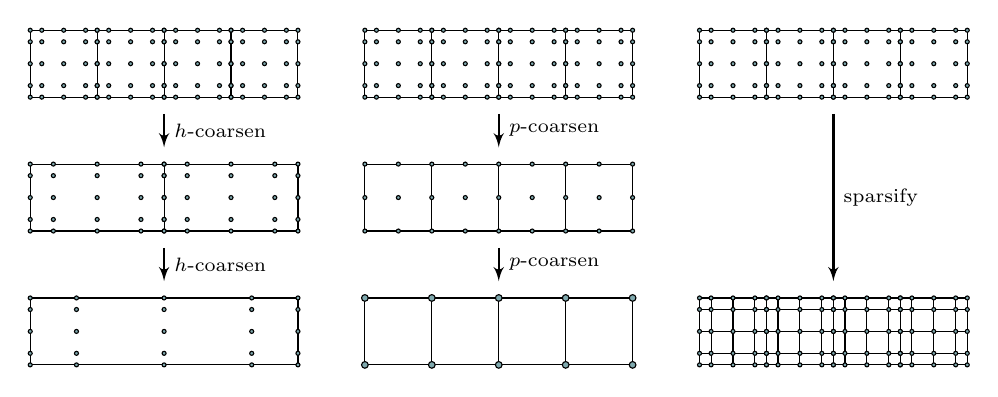
\begin{tikzpicture}[scale=0.85]
		% homg
		\draw (-5,4) grid +(4,1);
		\foreach \e in {-5,...,-2}
		\foreach \x in {0,0.1727,0.5,0.8273, 1.0} {
			\draw[fill=utsecblue] (\e+\x, 4) circle (0.03);
			\draw[fill=utsecblue] (\e+\x, 4.1727) circle (0.03);
			\draw[fill=utsecblue] (\e+\x, 4.5) circle (0.03);
			\draw[fill=utsecblue] (\e+\x, 4.8273) circle (0.03);
			\draw[fill=utsecblue] (\e+\x, 5) circle (0.03);
		}
		%\node at (5,4.5) {\small $p=4$};
		\draw[-latex',thick] (-3, 3.75) -- node[right] {{\scriptsize $h$-coarsen}} (-3, 3.25);
		\draw (-5,2) rectangle +(4,1);
		\draw (-3,2) -- (-3,3);
		\foreach \e in {-5,-3}
		\foreach \x in {0,0.1727,0.5,0.8273, 1.0} {
			\draw[fill=utsecblue] (\e+2*\x, 2) circle (0.03);
			\draw[fill=utsecblue] (\e+2*\x, 2.1727) circle (0.03);
			\draw[fill=utsecblue] (\e+2*\x, 2.5) circle (0.03);
			\draw[fill=utsecblue] (\e+2*\x, 2.8273) circle (0.03);
			\draw[fill=utsecblue] (\e+2*\x, 3) circle (0.03);
		}
		%\node at (5,2.5) {\small $p=2$};
	
		\draw[-latex',thick] (-3, 1.75) -- node[right] {{\scriptsize $h$-coarsen}} (-3, 1.25);
	
		\draw (-5,0) rectangle +(4,1);
		\foreach \x in {0,0.1727,0.5,0.8273, 1.0} {
			\draw[fill=utsecblue] (-5+4*\x, 0) circle (0.03);
			\draw[fill=utsecblue] (-5+4*\x, 0.1727) circle (0.03);
			\draw[fill=utsecblue] (-5+4*\x, 0.5) circle (0.03);
			\draw[fill=utsecblue] (-5+4*\x, 0.8273) circle (0.03);
			\draw[fill=utsecblue] (-5+4*\x, 1) circle (0.03);
		}
		
	%% p-multigrid
		\draw (0,4) grid +(4,1);
		\foreach \e in {0,...,3}
		\foreach \x in {0,0.1727,0.5,0.8273, 1.0} {
			\draw[fill=utsecblue] (\e+\x, 4) circle (0.03);
			\draw[fill=utsecblue] (\e+\x, 4.1727) circle (0.03);
			\draw[fill=utsecblue] (\e+\x, 4.5) circle (0.03);
			\draw[fill=utsecblue] (\e+\x, 4.8273) circle (0.03);
			\draw[fill=utsecblue] (\e+\x, 5) circle (0.03);
		}
		%\node at (5,4.5) {\small $p=4$};
	
		\draw[-latex',thick] (2, 3.75) -- node[right] {{\scriptsize $p$-coarsen}} (2, 3.25);
	
		\draw (0,2) grid +(4,1);
		\foreach \x in {0,0.5,...,4} {
			\draw[fill=utsecblue] (\x, 2) circle (0.03);
			\draw[fill=utsecblue] (\x, 2.5) circle (0.03);
			\draw[fill=utsecblue] (\x, 3) circle (0.03);
		}
		%\node at (5,2.5) {\small $p=2$};
	
		\draw[-latex',thick] (2, 1.75) -- node[right] {{\scriptsize $p$-coarsen}} (2, 1.25);
	
		\draw (0,0) grid +(4,1);
		\foreach \x in {0,1,2,3,4} {
			\draw[fill=utsecblue] (\x, 0) circle (0.05);
			\draw[fill=utsecblue] (\x, 1) circle (0.05);
		}
		%\node at (5,0.5) {\small $p=1$};
		
		%% collocated
			\draw (5,4) grid +(4,1);
			\foreach \e in {5,...,8}
			\foreach \x in {0,0.1727,0.5,0.8273, 1.0} {
				\draw[fill=utsecblue] (\e+\x, 4) circle (0.03);
				\draw[fill=utsecblue] (\e+\x, 4.1727) circle (0.03);
				\draw[fill=utsecblue] (\e+\x, 4.5) circle (0.03);
				\draw[fill=utsecblue] (\e+\x, 4.8273) circle (0.03);
				\draw[fill=utsecblue] (\e+\x, 5) circle (0.03);
			}
			%\node at (2, 1.8) {\tiny $p=4$};
	
			\draw[-latex',thick] (7, 3.75) -- node[right] {{\scriptsize sparsify}} (7, 1.25);
	
			\draw[step=0.5] (4.99,0) grid +(4.01,1);
			\draw (5,0.1727) -- (9,0.1727);
			\draw (5,0.8273) -- (9,0.8273);
			\foreach \e in {5,...,8} {
				\draw (\e+0.1727,0) -- (\e+0.1727,1);
				\draw (\e+0.8273,0) -- (\e+0.8273,1);
				\foreach \x in {0,0.1727,0.5,0.8273, 1.0} {
					\draw[fill=utsecblue] (\e+\x, 0) circle (0.03);
					\draw[fill=utsecblue] (\e+\x, 0.1727) circle (0.03);
					\draw[fill=utsecblue] (\e+\x, 0.5) circle (0.03);
					\draw[fill=utsecblue] (\e+\x, 0.8273) circle (0.03);
					\draw[fill=utsecblue] (\e+\x, 1) circle (0.03);
				}
			}
			% \node at (2, -0.2) {\tiny $p=1$ collocated with $p=4$};
		\end{tikzpicture}
		\caption{\label{fig:approaches} Different approaches
                  for high-order multigrid: high-order $h$-multigrid
                  (left), $p$-multigrid (middle) and low-order
                  multigrid based on the nodes of the nodes of the
                  high-order discretization, which can be used to
                  precondition the high-order system.}
\end{figure}

\subsubsection{$h$-multigrid}\label{subsec:h}
A direct approach to high-order multigrid is to use high-order
restriction and prolongation operators, and use the high-order
discretization of the operator for the residual computation on each
multigrid level (\S\ref{sub:restriction_&_prolongation}).
%A potential difficulty in this approach is that it
%requires smoothers for matrices arising from high-order
%discretization, which usually have less favorable properties compared
%to their low order counterparts; For instance, high-order
%discretizations of scalar elliptic operators are usually not
%M-matrices, which is a useful property to prove the convergence of
%smoothers such as Jacobi of Gauss-Seidel.
Due to the decreased sparsity of high-order discretized systems, the
efficient computation of the residual as well as devising efficient
smoothers can be a challenge. As a remedy, one can use matrix-free
methods which do not require to assemble system matrices but rely on
element-local computations. The performance of these element-local
computations can often be speed up using tensorized finite element
basis functions as common in spectral element methods; see
e.g.~\cite{DevilleFischerMund02}. 

\subsubsection{$p$-multigrid}\label{subsec:p}
In the $p$-multigrid approach to high-order multigrid, one (initially)
does not coarsen the mesh geometrically, but coarsens the finite
element system by
reducing the polynomial order. Starting from an order-$p$ polynomial
basis (for simplicity, we assume here that $p$ is a power of 2), the
coarser grids correspond to polynomials of order $p/2, p/4,\ldots,1$,
followed by geometric coarsening of the $p=1$ grid (i.e., the standard
low-order geometric multigrid). 
%Decreasing the polynomial order is an element-local operation and is particularly simple for discretizations with nonconforming meshes. \gsnote{Is that actually true?}. 
As for high-order $h$-multigrid, devising smoothers can be a challenge for
$p$-multigrid.  Moreover, one often finds dependence of the
convergence factor on the order of the polynomial basis
\cite{MadayMunoz89}.

\subsubsection{Preconditioning using AMG hierarchy of lower-order operator} \label{subsec:low}
In this defect correction approach (see
\cite{TrottenbergOosterleeSchuller01, Hackbusch85}), the high-order
defect/residual is iteratively corrected using a low order operator
obtained by overlaying the high-order nodes with a low order
(typically linear) finite element mesh. While the resulting low-order
operator has the same number of degrees of freedom as the high-order
operator, it is much sparser and can thus be assembled efficiently and
then provided as input to an algebraic multigrid method, which
computes a grid hierarchy through algebraic point aggregation.  This
construction of a low-order preconditioner based on the nodes of the
high-order discretization is used, for instance in~\cite{Brown10,
  Kim07, DevilleMund90, HeysManteuffelMcCormickEtAl05}.  Due to the
black-box nature of algebraic multigrid, it is particularly attractive
for high-order discretizations on unstructured meshes.  Even for
structured meshes, the solution of the low-order system with a
geometric multigrid method is not straightforward due to the non
evenly spaced node points inherited from the high-order
discretization.  In principle, this approach only requires computation
of the residual for the high-order discretized operator. Smoothing on
the finest level uses the low-order discretized operator, and either
the high-order or the low-order residual can be used in the
smoother. Using the high-order residual in the smoother requires an
additional high-order residual computation per smoothing step.


% The resulting method is nearly independent of $p$, but this low-order
% preconditioning is not work optimal and the convergence factors can be
% lower than when multigrid is applied directly to the high-order
% operator. \gsnote{Reference or remove statement.} 


% and the
%fact that the low-order system matrix is sparse and can thus be
%assembled efficiently.
%, where the construction of a
%grid hierarchy from geometric coarsening can be very difficult.
% For structured grids such as the ones used for
% the test problems in Section~\ref{sec:numerics}, a geometric multigrid
% method can be devised that either copes with the non evenly spaced
% points (which can be challenging) or replaces them by evenly spaced
% points---we experiment with the latter option in
% Section~\ref{sec:numerics}.

% multigrid cycles are faster compared to high
%order $h$-multigrid or $p$-multigrid discussed in
%Section~\ref{subsec:h} and Section~\ref{subsec:p}, respectively.

%Standard multigrid is then used for the low order operator, which has
%more favorable sparsity properties and thus allows for standard
%smoothers.
%  Thus, the speedup for a full multigrid cycle when using the
%low order operator is limited.

%The advantages of doing
%this are mainly in the simplicity of the approach and the availability
%of parallel multigrid solvers capable of solving such lower-order
%operators.
% The sparsity of the lower-order operators also permits the
%use of AMG for solving the lower-order operators, possibly obtained
%via discretizations on unstructured meshes.


% **********************************************************
\subsection{Smoothers}\label{subsec:smoothers}
Next, we summarize different smoothing approaches. In our numerical
comparisons, we restrict ourselves to the point smoothers reviewed in
\S\ref{subsec:ptsmoothers}. For completeness of the
presentation, we briefly describe Schwarz-type smoothers in
\S\ref{subsec:schwarz}.


\subsubsection{Point smoothers}\label{subsec:ptsmoothers}
In our numerical tests, we compare the Jacobi and the symmetric successive over
relaxation (SSOR) smoothers, as well as a Chebyshev-accelerated Jacobi
smoother~\cite{Brandt77}. All of these smoothers require the diagonal of the
system matrix; if matrices are not assembled (i.e., in a matrix-free approach),
these diagonal entries must be precomputed in a setup step.  Note that the
parallelization of Gauss-Seidel smoothers (such as SSOR) requires coloring of
unknowns at parallel boundaries, and, compared to Jacobi smoothing, more
complex communication in a distributed memory implementation. The
Chebyshev-accelerated Jacobi method is an attractive alternative to SSOR; it
can significantly improve over Jacobi smoothing, while being as simple to
implement~\cite{AdamsBrezinaHuEtAl03}. The acceleration of Jacobi smoothing
with Chebyshev polynomials requires estimation of the maximum eigenvalues of
the system matrix, which has to be done in a setup. For our experiments, we
estimated the largest eigenvalue using 10 iterations of the Arnoldi algorithm.

In Figures~\ref{fig:smoothers} and~\ref{fig:smoothers-var}, we compare the
efficiency of these point smoothers for different polynomial orders. In our
tests, we compute the eigenvectors of the system matrix, choose a zero right
hand side and an initialization that has all unit coefficients in the basis
given by these eigenvectors. For the polynomial orders $p=1,4,16$, we compare
the performance of point smoothers with and without a multigrid step.  We
depict the coefficients after 6 smoothing steps on the left, and the results
obtained for a two-grid method\footnote{For simplicity, we chose two grids in
our tests; the results for a multigrid v-cycle are very similar.} with 3 pre
and 3 post smoothing steps (and thus overall 6 smoothing steps on the finest
grid) on the left. The SSOR smoother uses a lexicographic ordering of the
unknowns, and we use 2 pre and 1 post smoothing steps, which again amounts to
overall 6 smoothing steps on the finest grid. The Chebyshev smoother targets
the part of the spectrum given by $[\lambda_\text{max}/4,\lambda_\text{max}]$,
where $\lambda_\text{max}$ is the maximum eigenvalue of the system matrix. 

The results for the constant coefficient Laplacian operator on the
unit square (Figure~\ref{fig:smoothers}) show that all point
smoothers decrease the error compoments in the upper half of the
spectrum, but that this damping factor is smaller for high-order
elements. Note that Chebyshev accelerated Jacobi smoothing results in
a uniform damping of a larger part of the spectrum than Jacobi
smoothing.  Both, the Chebyshev and SSOR methods outperform Jacobi
smoothing, in particular for higher orders. Combining the smoothers
with a two-grid cycle, all error components are decreased for all
smoothers (and thus the resulting two-grid methods converge, see
Table~\ref{tab:box} in the section summarizing our numerical tests),
but the error decreases slower for higher polynomial degrees. For high
polynomial order, a two-grid iteration with SSOR smoothing results in a
significantly better error reduction than Jacobi or Chebyshev
smoothing.

In Figure~\ref{fig:smoothers-var}, we study the solution of
\eqref{eq:Poisson} with a smoothly (but highly) varying coefficient
$\mu$ on a deformed geometry. Note that, comparing with the constant
coefficient case, now Jacobi smoothing performs significantly worse,
both, when used as a solver and as a smoother. In particular, for
$p=16$ Jacobi smoothing does not lead to a converging two-grid
algorithm (compare with Table~\ref{tab:2d-fan}). SSOR smoothing
combined with the two-grid method still retains a satisfactory
convergence rate. \todo{Hari, Chebyshev-based multigrid also seems to
  have values larger than 1 but seems to converge in the tables in the
  back...any idea why?}

\begin{figure}
	\centering
		\begin{tikzpicture}[scale=0.8]
		\begin{semilogyaxis}[ymajorgrids,ymin=1e-5,ymax=2,xmin=0,xmax=961]
		\addplot[color=black]  table[x=dof, y=u]{data/smoother-const-box.dat};
		\addplot[color=blue!70, opacity=0.5,only marks, mark=*,mark size=1pt]   table[x=dof, y=jacobi1]{data/smoother-const-box.dat};
		\addplot[color=red!70!black, opacity=0.5,only marks, mark=*,mark size=1pt] table[x=dof, y=chebyshev1]{data/smoother-const-box.dat};
		\addplot[color=green!70!black,only marks, opacity=0.5,mark=*,mark size=1pt]  table[x=dof, y=ssor1]{data/smoother-const-box.dat};
		\end{semilogyaxis}
		\draw[black, fill=white] (4.0, 3.7) rectangle +(2.85,2);
		% \draw[black] (4.0, 5.375) -- (6.85,5.375);
		\node at (5.35, 5.53) {\bf \small{smooth, $p=1$}}; 
		\node[fill=blue!70, draw, circle,minimum width=0.1cm] at (4.3, 5.0) {}; 
		\node[fill=red!70!black, draw, circle,minimum width=0.1cm] at (4.3, 4.5) {};
		\node[fill=green!70!black, draw, circle,minimum width=0.1cm] at (4.3, 4.0) {};
		\node[text width=1.9cm] at (5.75, 5.0) {\small jacobi $(6)$};
		\node[text width=1.9cm] at (5.75, 4.5) {\small chebyshev $(6)$};
		\node[text width=1.9cm] at (5.75, 4.0) {\small ssor $(3)$};
		\end{tikzpicture}
		\begin{tikzpicture}[scale=0.8]
		\begin{semilogyaxis}[ymajorgrids,ymin=1e-5,ymax=2,xmin=0,xmax=961,yticklabels={,,}]
		\addplot[color=black]  table[x=dof, y=u]{data/vcycle-const-box.dat};
		\addplot[color=blue!70,opacity=0.5,only marks, mark=*,mark size=1pt]   table[x=dof, y=jacobi1]{data/vcycle-const-box.dat};
		\addplot[color=red!70!black,opacity=0.5,only marks, mark=*,mark size=1pt] table[x=dof, y=chebyshev1]{data/vcycle-const-box.dat};
		\addplot[color=green!70!black,opacity=0.5,only marks, mark=*,mark size=1pt]  table[x=dof, y=ssor1]{data/vcycle-const-box.dat};
		\end{semilogyaxis}
		\draw[black, fill=white] (3.7, 3.7) rectangle +(3.15,2);
		%\draw[black] (4.0, 5.375) -- (6.85,5.375);
		\node at (5.35, 5.53) {\bf \small{v-cycle, $p=1$}}; 
		\node[fill=blue!70, draw, circle,minimum width=0.1cm] at (4.0, 5.0) {}; 
		\node[fill=red!70!black, draw, circle,minimum width=0.1cm] at (4.0, 4.5) {};
		\node[fill=green!70!black, draw, circle,minimum width=0.1cm] at (4.0, 4.0) {};
		\node[text width=2.1cm] at (5.55, 5.0) {\small jacobi $(3,3)$};
		\node[text width=2.1cm] at (5.55, 4.5) {\small chebyshev $(3,3)$};
		\node[text width=2.1cm] at (5.55, 4.0) {\small ssor $(2,1)$};
		\end{tikzpicture}
	\\
		\begin{tikzpicture}[scale=0.8]
		\begin{semilogyaxis}[ymajorgrids,ymin=1e-5,ymax=2,xmin=0,xmax=961]
		\addplot[color=black]  table[x=dof, y=u]{data/smoother-const-box.dat};
		\addplot[color=blue!70,opacity=0.5,only marks, mark=*,mark size=1pt]   table[x=dof, y=jacobi4]{data/smoother-const-box.dat};
		\addplot[color=red!70!black,opacity=0.5,only marks, mark=*,mark size=1pt] table[x=dof, y=chebyshev4]{data/smoother-const-box.dat};
		\addplot[color=green!70!black,opacity=0.5,only marks, mark=*,mark size=1pt]  table[x=dof, y=ssor4]{data/smoother-const-box.dat};
		\end{semilogyaxis}
		\draw[black, fill=white] (4.0, 5.375) rectangle +(2.85,0.325);
		\node at (5.35, 5.53) {\bf \small{smooth, $p=4$}};
		\end{tikzpicture}
		\begin{tikzpicture}[scale=0.8]
		\begin{semilogyaxis}[ymajorgrids,ymin=1e-5,ymax=2,xmin=0,xmax=961,yticklabels={,,}]
		\addplot[color=black]  table[x=dof, y=u]{data/vcycle-const-box.dat};
		\addplot[color=blue!70,only marks,opacity=0.5, mark=*,mark size=1pt]   table[x=dof, y=jacobi4]{data/vcycle-const-box.dat};
		\addplot[color=red!70!black,only marks,opacity=0.5, mark=*,mark size=1pt] table[x=dof, y=chebyshev4]{data/vcycle-const-box.dat};
		\addplot[color=green!70!black,only marks,opacity=0.5, mark=*,mark size=1pt]  table[x=dof, y=ssor4]{data/vcycle-const-box.dat};
		\end{semilogyaxis}
			\draw[black, fill=white] (4.0, 5.375) rectangle +(2.85,0.325);
			\node at (5.35, 5.53) {\bf \small{v-cycle, $p=4$}};
		\end{tikzpicture}
	\\
		\begin{tikzpicture}[scale=0.8]
		\begin{semilogyaxis}[ymajorgrids,ymin=1e-5,ymax=2,xmin=0,xmax=961]
		\addplot[color=black]  table[x=dof, y=u]{data/smoother-const-box.dat};
		\addplot[color=blue!70,opacity=0.5,only marks, mark=*,mark size=1pt]   table[x=dof, y=jacobi16]{data/smoother-const-box.dat};
		\addplot[color=red!70!black,opacity=0.5,only marks, mark=*,mark size=1pt] table[x=dof, y=chebyshev16]{data/smoother-const-box.dat};
		\addplot[color=green!70!black,opacity=0.5,only marks, mark=*,mark size=1pt]  table[x=dof, y=ssor16]{data/smoother-const-box.dat};
		\end{semilogyaxis}
		\draw[black, fill=white] (3.9, 5.375) rectangle +(2.95,0.325);
		\node at (5.35, 5.53) {\bf \small{smooth, $p=16$}};
		\end{tikzpicture}
		\begin{tikzpicture}[scale=0.8]
		\begin{semilogyaxis}[ymajorgrids,ymin=1e-5,ymax=2,xmin=0,xmax=961,yticklabels={,,}]
		\addplot[color=black]  table[x=dof, y=u]{data/vcycle-const-box.dat};
		\addplot[color=blue!70,opacity=0.5,only marks, mark=square*,mark size=1pt]   table[x=dof, y=jacobi16]{data/vcycle-const-box.dat};
		\addplot[color=red!70!black,opacity=0.4,only marks, mark=*,mark size=1pt] table[x=dof, y=chebyshev16]{data/vcycle-const-box.dat};
		\addplot[color=green!70!black,opacity=0.6,only marks, mark=diamond*,mark size=1pt]  table[x=dof, y=ssor16]{data/vcycle-const-box.dat};
		\end{semilogyaxis}
		\draw[black, fill=white] (3.95, 5.375) rectangle +(2.9,0.325);
		\node at (5.35, 5.53) {\bf \small{v-cycle, $p=16$}};
		\end{tikzpicture}
	\caption{\label{fig:smoothers} Error decay for different
          point smoothers when used as solver (left column) and when used
          within a single two-grid step (right column) for a two-dimensional,
          constant coefficient Laplace problem on a unit square. To
          keep the number of unknowns the same for
          different polynomial orders, meshes of $32\times 32$,
          $8\times 8$ and $2\times 2$ elements are used for polynomial
          orders $p=1$, $p=4$ and $p=16$, respectively.
          Plotted are the coefficients of the error
          expanded in the eigenvectors of the system matrix $A_k$.
          The order of the eigenvectors is such that the
          corresponding eigenvalues are descending; thus, the
          smoothness of the eigenvectors decays from left to right.
          The initialization is chosen to have all unit coefficients in
          the eigenvector expansion.}
\end{figure}

%% Variable Coefficients ----- SHELL

\begin{figure}
	\centering
		\begin{tikzpicture}[scale=0.8]
		\begin{semilogyaxis}[ymajorgrids,ymin=1e-5,ymax=2,xmin=0,xmax=961]
		\addplot[color=black]  table[x=dof, y=u]{data/smoother-var-shell.dat};
		\addplot[color=blue!70, opacity=0.5,only marks, mark=*,mark size=1pt]   table[x=dof, y=jacobi1]{data/smoother-var-shell.dat};
		\addplot[color=red!70!black, opacity=0.5,only marks, mark=*,mark size=1pt] table[x=dof, y=chebyshev1]{data/smoother-var-shell.dat};
		\addplot[color=green!70!black,only marks, opacity=0.5,mark=*,mark size=1pt]  table[x=dof, y=ssor1]{data/smoother-var-shell.dat};
		\end{semilogyaxis}
		\draw[black, fill=white] (4.0, 3.7) rectangle +(2.85,2);
		\node at (5.35, 5.53) {\bf \small{smooth, $p=1$}}; 
		\node[fill=blue!70, draw, circle,minimum width=0.1cm] at (4.3, 5.0) {}; 
		\node[fill=red!70!black, draw, circle,minimum width=0.1cm] at (4.3, 4.5) {};
		\node[fill=green!70!black, draw, circle,minimum width=0.1cm] at (4.3, 4.0) {};
		\node[text width=1.9cm] at (5.75, 5.0) {\small jacobi $(6)$};
		\node[text width=1.9cm] at (5.75, 4.5) {\small chebyshev $(6)$};
		\node[text width=1.9cm] at (5.75, 4.0) {\small ssor $(3)$};
		\end{tikzpicture}
		\begin{tikzpicture}[scale=0.8]
		\begin{semilogyaxis}[ymajorgrids,ymin=1e-5,ymax=2,xmin=0,xmax=961,yticklabels={,,}]
		\addplot[color=black]  table[x=dof, y=u]{data/vcycle-var-shell.dat};
		\addplot[color=blue!70,opacity=0.5,only marks, mark=*,mark size=1pt]   table[x=dof, y=jacobi1]{data/vcycle-var-shell.dat};
		\addplot[color=red!70!black,opacity=0.5,only marks, mark=*,mark size=1pt] table[x=dof, y=chebyshev1]{data/vcycle-var-shell.dat};
		\addplot[color=green!70!black,opacity=0.5,only marks, mark=*,mark size=1pt]  table[x=dof, y=ssor1]{data/vcycle-var-shell.dat};
		\end{semilogyaxis}
		\draw[black, fill=white] (3.7, 3.7) rectangle +(3.15,2);
		\node at (5.35, 5.53) {\bf \small{v-cycle, $p=1$}}; 
		\node[fill=blue!70, draw, circle,minimum width=0.1cm] at (4.0, 5.0) {}; 
		\node[fill=red!70!black, draw, circle,minimum width=0.1cm] at (4.0, 4.5) {};
		\node[fill=green!70!black, draw, circle,minimum width=0.1cm] at (4.0, 4.0) {};
		\node[text width=2.1cm] at (5.55, 5.0) {\small jacobi $(3,3)$};
		\node[text width=2.1cm] at (5.55, 4.5) {\small chebyshev $(3,3)$};
		\node[text width=2.1cm] at (5.55, 4.0) {\small ssor $(2,1)$};
		\end{tikzpicture}
	\\
		\begin{tikzpicture}[scale=0.8]
		\begin{semilogyaxis}[ymajorgrids,ymin=1e-5,ymax=2,xmin=0,xmax=961]
		\addplot[color=black]  table[x=dof, y=u]{data/smoother-var-shell.dat};
		\addplot[color=blue!70,opacity=0.5,only marks, mark=*,mark size=1pt]   table[x=dof, y=jacobi4]{data/smoother-var-shell.dat};
		\addplot[color=red!70!black,opacity=0.5,only marks, mark=*,mark size=1pt] table[x=dof, y=chebyshev4]{data/smoother-var-shell.dat};
		\addplot[color=green!70!black,opacity=0.5,only marks, mark=*,mark size=1pt]  table[x=dof, y=ssor4]{data/smoother-var-shell.dat};
		\end{semilogyaxis}
		\draw[black, fill=white] (4.0, 5.375) rectangle +(2.85,0.325);
		\node at (5.35, 5.53) {\bf \small{smooth, $p=4$}};
		\end{tikzpicture}
		\begin{tikzpicture}[scale=0.8]
		\begin{semilogyaxis}[ymajorgrids,ymin=1e-5,ymax=2,xmin=0,xmax=961,yticklabels={,,}]
		\addplot[color=black]  table[x=dof, y=u]{data/vcycle-var-shell.dat};
		\addplot[color=blue!70,only marks, mark=*,opacity=0.5,mark size=1pt]   table[x=dof, y=jacobi4]{data/vcycle-var-shell.dat};
		\addplot[color=red!70!black,only marks, mark=*,opacity=0.5,mark size=1pt] table[x=dof, y=chebyshev4]{data/vcycle-var-shell.dat};
		\addplot[color=green!70!black,only marks, mark=*,opacity=0.5,mark size=1pt]  table[x=dof, y=ssor4]{data/vcycle-var-shell.dat};
		\end{semilogyaxis}
		\draw[black, fill=white] (4.0, 5.375) rectangle +(2.85,0.325);
		\node at (5.35, 5.53) {\bf \small{v-cycle, $p=4$}};
		\end{tikzpicture}
	\\
		\begin{tikzpicture}[scale=0.8]
		\begin{semilogyaxis}[ymajorgrids,ymin=1e-5,ymax=2,xmin=0,xmax=961]
		\addplot[color=black]  table[x=dof, y=u]{data/smoother-var-shell.dat};
		\addplot[color=blue!70,opacity=0.5,only marks, mark=*,mark size=1pt]   table[x=dof, y=jacobi16]{data/smoother-var-shell.dat};
		\addplot[color=red!70!black,opacity=0.5,only marks, mark=*,mark size=1pt] table[x=dof, y=chebyshev16]{data/smoother-var-shell.dat};
		\addplot[color=green!70!black,opacity=0.5,only marks, mark=*,mark size=1pt]  table[x=dof, y=ssor16]{data/smoother-var-shell.dat};
		\end{semilogyaxis}
		\draw[black, fill=white] (3.9, 5.375) rectangle +(2.95,0.325);
		\node at (5.35, 5.53) {\bf \small{smooth, $p=16$}};
		\end{tikzpicture}
		\begin{tikzpicture}[scale=0.8]
		\begin{semilogyaxis}[ymajorgrids,ymin=1e-5,ymax=2,xmin=0,xmax=961,yticklabels={,,}]
		\addplot[color=black]  table[x=dof, y=u]{data/vcycle-var-shell.dat};
		\addplot[color=blue!70,opacity=0.5,only marks, mark=square*,mark size=1pt]   table[x=dof, y=jacobi16]{data/vcycle-var-shell.dat};
		\addplot[color=red!70!black,opacity=0.5,only marks, mark=*,mark size=1pt] table[x=dof, y=chebyshev16]{data/vcycle-var-shell.dat};
		\addplot[color=green!70!black,opacity=0.5,only marks, mark=diamond*,mark size=1pt]  table[x=dof, y=ssor16]{data/vcycle-var-shell.dat};
		\end{semilogyaxis}
		\draw[black, fill=white] (3.95, 5.375) rectangle +(2.9,0.325);
		\node at (5.35, 5.53) {\bf \small{v-cycle, $p=16$}};
		\end{tikzpicture}
	\caption{\label{fig:smoothers-var} Same as
          Figure~\ref{fig:smoothers}, but for the two-dimensional warped
          geometry shown in Figure~\ref{fig:mesh} with varying coefficient
          $\mu(x,y) = 1 + 10^6(\cos^2(2\pi x) + \cos^2(2\pi y))$.}
\end{figure}


\subsubsection{Schwarz-based smoothers}\label{subsec:schwarz}
An alternative smoothing approach for high-order discretizations is
based on local block solves.  Schwarz-type domain decomposition
smoothers have successfully been used for spectral element
discretizations with orders significantly higher than 8. They are more
stable for anisotropic meshes or anisotropic problems than point
smoothers. A main challenge of Schwarz-type smoothers is that they
require the solution of dense local systems.  This is either done by
using direct methods or approximations that allow for a fast iterative
solution \cite{LottesFischer05, FischerLottes05}. However, the
coarse-grid solves can become fairly expensive. Moreover, depending on
how much overlap between the domains is used, it is not
straightforward to achieve good parallel scalability.

\subsection{Comparing computational cost}\label{subsec:complexity}
To compare the computational cost of the different methods, we focus
on matrix-vector multiplications on the finest multigrid level, which
dominate the overall computation. Denoting the number of unknowns on
the finest level by $N$, the cost for a matrix-vector product is
$Ng_p$, where $g_p>0$ is the cost per unknown for the application of
an operator originating from a discretization with polynomial order
$p$. Since high-order discretizations result in less sparse operators,
we have $g_1\le g_2\le \ldots$. The actual value of $g_p$ depends
strongly on the implementation and on the system architecture.
% To
%illustrate this, consider an elemental matrix for a hexahedral mesh in
%three dimensions, which is dense and of size $(p+1)^3\times
%(p+1)^3$. Its naive application to a vector amounts to $\mathcal
%O((p+1)^6)$ operations; for tensor bases, as common in spectral
%element methods, this can be reduced to $\mathcal O((p+1)^4)$
%operations \cite{DevilleFischerMund02}.
In general, high-order implementations allow more memory locality,
which often results in higher performance compared to low order
methods.

The dominant computational cost per iteration of the high-order
multigrid approaches discussed in \S\ref{sec:approaches} can
thus be summarized as
\begin{equation}\label{eq:compcost}
  g_p(1+m(s_\text{pre}+s_\text{post})).
\end{equation}
Here, we denote by $s_\text{pre}$ and $s_\text{post}$ the number of
pre and post smoothing steps on the finest multigrid level,
respectively. Moreover, $m$ denotes the number of necessary residual
computations (and thus matrix-vector computations) per smoothing step.
Jacobi smoothing and Chebyshev-accelerated Jacobi require $m=1$
matrix-vector multiplication per smoothing step, while SSOR requires
$m=2$ matrix-vector operations. If, in the approach discussed in
\S\ref{subsec:low}, the linear-order residual is used in the
smoother, then the cost \eqref{eq:compcost} reduces to
\begin{equation}\label{eq:compcost2}
  g_p+g_1m(s_\text{pre}+s_\text{post})).
\end{equation}
However, since the overall number of iterations increases (see
\S\ref{subsec:results}), this usually does not decrease the
solution time.

% note that  Jacobi, SSOR and
%Chebyshev-accelerated Jacobi require a matrix-vector product, and we
%denote by $m$ the number of such products per smoothing step.


%\begin{itemize}
%\item {\em high-order $h$-multigrid:} On the finest grid level, the
%  residual and the smoothing steps are all based on the order $p$
%  discretization. Thus, the cost based on the matrix-vector products
%  on the finest multigrid level is
%  $g_p(1+m(s_\text{pre}+s_\text{post}))$.
%
%\item {\em $p$-multigrid:} As for high-order $h$-multigrid, an
%  estimate for the computational cost on the finest level is
%  $g_p(1+m(s_\text{pre}+s_\text{post}))$.
%
%\item {\em high-order defect correction with linear-order operator:}
%  high-order defect correction requires the computation of the
%  high-order residual, but uses smoothing based on the low-order
%  operator. Using linear elements, the computational cost on the
%  finest grid level is thus
%  $g_p(1+m(s_\text{pre}+s_\text{post}))$.
%\end{itemize}


If the overall number of unknowns $N$ is kept fixed and the problem
solution is smooth, it is well known that the accuracy increases for
high-order discretizations. Due to the decreased sparsity of the
discretized operators, this does not automatically translate into more
accuracy per computation time; see, e.g.~\cite{Brown10}. However, note
that the complexity of most computations in a multigrid preconditioned
conjugate gradient algorithm, for instance, are of complexity
$\mathcal{O}(N)$ (see Algorithm~\ref{alg:pcg}) and thus independent of
$g_p$. Thus, the computational cost of these steps does not depend on
the order of the discretization. Even if these $\mathcal{O}(N)$ steps
do not dominate the computation, they contribute to making high-order
discretizations favorable not only in terms of accuracy per unknown,
but also in terms of accuracy per computation time.

\begin{algorithm}[ht] 
  % v-cycle 
  \caption{Multigrid preconditioned Conjugate Gradient Method} \label{alg:pcg} 
  \begin{algorithmic}[1]
    \Require rhs and guess
    \Ensure  solution
    \While {not converged} 
    \State $\bs{h} = A \bs{p}$ 											\Comment $~~\quad\quad\quad\quad\mathcal{O}(Ng_p)$
    \State $\rho_r = (\rho, \bs{r})$								\Comment $~~\quad\quad\quad\quad\mathcal{O}(N)~~~$
    \State $\alpha = \rho_r / ( \bs{p}, \bs{h} )$		\Comment $~~\quad\quad\quad\quad\mathcal{O}(N)~~~$
    \State $\bs{u} = \bs{u} + \alpha\bs{p}$					\Comment $~~\quad\quad\quad\quad\mathcal{O}(N)~~~$
    \State $\bs{r} = \bs{r} - \alpha\bs{h}$					\Comment $~~\quad\quad\quad\quad\mathcal{O}(N)~~~$
    \State Convergence Test
    \State $\rho = M\bs{r}$ 												\Comment V-cycle $\quad\mathcal{O}(Ng_p)$
    \State $\beta = (\rho, \bs{r}) / \rho_r$				\Comment $~~\quad\quad\quad\quad\mathcal{O}(N)~~~$
    \State $\bs{p} = \rho + \beta\bs{p}$						\Comment $~~\quad\quad\quad\quad\mathcal{O}(N)~~~$
    \EndWhile
  \end{algorithmic}
\end{algorithm}




% **************************************************
% **************************************************
\section{Numerical results}\label{sec:numerics}
In this section we present a comprehensive comparison of our
algorithms for the solution of high-order discretizations of
\eqref{eq:Poisson}.  After introducing our test problems in
\S\ref{subsec:tests}, in \S\ref{subsec:measures} we
describe how we compare our methods for high-order multigrid. The
results for our test problem are then presented and discussed
\S\ref{subsec:results}.


\subsection{Presentation of test problems}\label{subsec:tests}
We compare our algorithms for the solution of~\eqref{eq:Poisson} on a
unit square and a unit cube with constant coefficient $\mu\equiv 1$,
as well as on the warped two and three dimensional domains shown in
Figure~\ref{fig:mesh}, where we use a varying coefficient $\mu(\bs
x)$. 
% \todo{How anisotropic is the 2d-fan mesh? Probably we also have to update the mesh plots.}  
We use isoparametric elements for these
deformed geometries, i.e., the geometry transformation is approximated
using the same polynomial order as the finite element functions. The
Jacobians for this transformation are computed at every quadrature
point. The coefficient $\mu$ at the coarse grid quadrature points is
computed as the linear interpolation of the coefficient at the fine
grid quadrature points. In our tests, we change the polynomial degree of
the finite element functions but keep the same mesh; this results in
an increasing number of unknowns as $p$ increases. It is important to 
point out that mesh independence is acheived for all $p$, therefore
the results are similar for larger mesh sizes as well.

\begin{figure}
	% 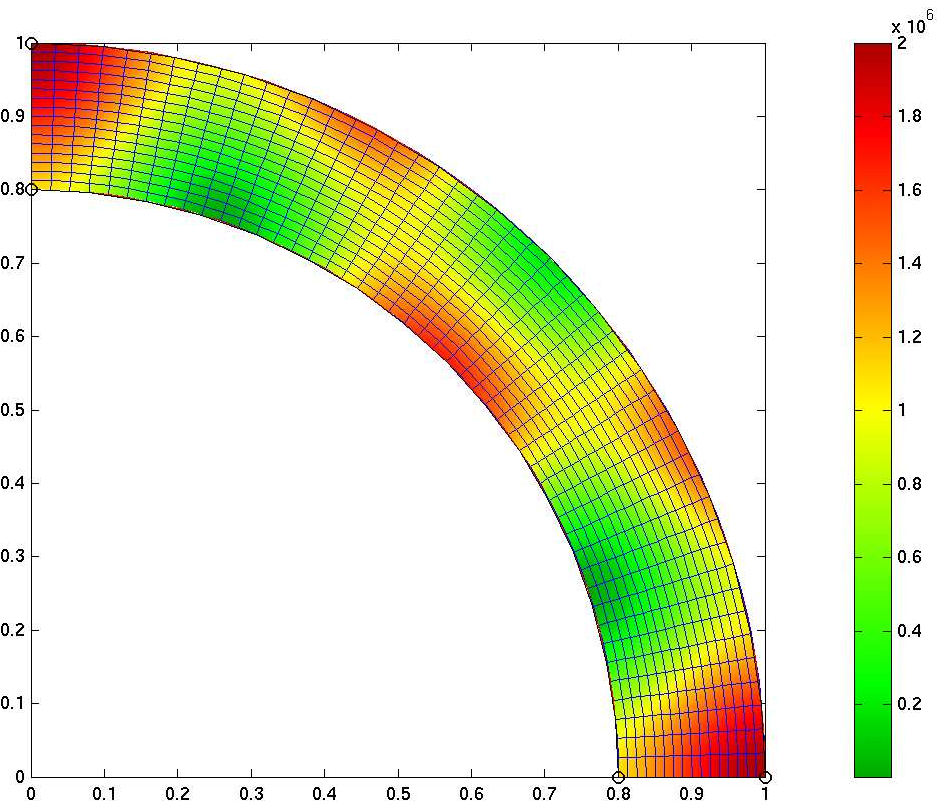
\includegraphics[width=0.48\textwidth]{figs/fan}
	% This file was created by matlab2tikz v0.3.3.
% Copyright (c) 2008--2013, Nico Schlömer <nico.schloemer@gmail.com>
% All rights reserved.
% 
% 
% 
\begin{tikzpicture}

\begin{axis}[%
width=1.8in,
height=2.0in,
view={0}{90},
scale only axis,
xmin=0,
xmax=0.8,
% xmajorgrids,
ymin=0.55,
ymax=1.05,
% ymajorgrids,
zmin=-1,
zmax=1,
% zmajorgrids,
axis x line*=bottom,
axis y line*=left,
axis z line*=left,
colormap/jet,
%colormap={traffic}{color(0cm)=(green); color(1cm)=(yellow); color(2cm)=(red)},
colorbar,
colorbar style={%title=$\mu$,
        width=0.15in, height=1.4in,
				at={(1.1,0.5)},anchor=east
    },
point meta min=3687.27158757943,
point meta max=2000001
]

\addplot3[%
surf,
colormap/jet,
%colormap={traffic}{color(0cm)=(green); color(1cm)=(yellow); color(2cm)=(red)},
shader=flat,
z buffer=sort,
point meta=explicit,
mesh/rows=65]
table[row sep=crcr,meta index=3,header=false] {
0 0.8 0 1095492.50281253\\
0.00981723062857594 0.799939761471316 0 1091470.11955702\\
0.0196329828183298 0.799759054956964 0 1079464.42475455\\
0.0294457783530871 0.79945790767068 0 1059658.73790523\\
0.0392541394619344 0.799036364964138 0 1032355.12786921\\
0.0490565890417669 0.79849449032012 0 997969.290417877\\
0.058851650879734 0.797832365342952 0 957023.521077331\\
0.0686378498755519 0.797050089746223 0 910137.92349953\\
0.0784137122636485 0.796147781337758 0 858020.028016915\\
0.0881777658351065 0.795125576001885 0 801453.025429382\\
0.097928540159373 0.793983627678968 0 741282.846764197\\
0.107664566805701 0.792722108342224 0 678404.340190066\\
0.117384379564289 0.791341207971825 0 613746.81104152\\
0.127086514667089 0.789841134526287 0 548259.199750399\\
0.136769511008241 0.788222113911153 0 482895.175268579\\
0.146431910364113 0.786484389944973 0 418598.418333033\\
0.156072257612903 0.784628224322584 0 356288.359850942\\
0.165689100953775 0.782653896575702 0 296846.625089343\\
0.175280992125496 0.780561704030823 0 241104.414690027\\
0.184846486624537 0.778351961764448 0 189831.029359803\\
0.194384143922611 0.776025002555635 0 143723.717069281\\
0.203892527683612 0.773581176835882 0 103398.990467864\\
0.213370205979919 0.771020852636352 0 69385.5287825629\\
0.222815751508043 0.768344415532453 0 42118.74354135\\
0.23222774180357 0.765552268585767 0 21937.051887418\\
0.241604759455383 0.762644832283355 0 9079.86585794335\\
0.250945392319113 0.759622544474429 0 3687.27158757943\\
0.26024823372981 0.756485860304417 0 5801.33971023018\\
0.269511882713776 0.753235252146417 0 15368.9779524042\\
0.278734944199548 0.74987120953006 0 32246.2096351285\\
0.287916029227991 0.746394239067791 0 56203.7380324736\\
0.29705375516147 0.742804864378573 0 86933.6366739991\\
0.306146745892072 0.739103626009029 0 124056.990018216\\
0.315193632048839 0.735291081352046 0 167132.297646148\\
0.324193051203992 0.731367804562825 0 215664.448299602\\
0.33314364807811 0.727334386472418 0 269114.067682562\\
0.342044074744226 0.723191434498755 0 326907.045820135\\
0.350892990830822 0.718939572555163 0 388444.055699444\\
0.359689063723685 0.714579440956412 0 453109.884590414\\
0.368430968766592 0.710111696322283 0 520282.412480874\\
0.377117389460798 0.705537011478684 0 589341.08802169\\
0.385747017663298 0.700856075356325 0 659674.770781799\\
0.394318553783827 0.696069592886969 0 730688.828947614\\
0.402830706980574 0.69117828489727 0 801811.403337476\\
0.411282195354577 0.686182888000218 0 872498.771206958\\
0.419671746142775 0.681084154484212 0 942239.766270842\\
0.427998095909678 0.675882852199766 0 1010559.23415821\\
0.436259990737637 0.670579764443871 0 1077020.52467328\\
0.444456186415682 0.665175689842036 0 1141227.0433196\\
0.452585448626891 0.65967144222802 0 1202822.9041664\\
0.460646553134276 0.654067850521267 0 1261492.74395132\\
0.468638285965151 0.648365758602076 0 1316960.77303442\\
0.476559443593947 0.642566025184516 0 1368989.15221189\\
0.48440883312346 0.636669523687107 0 1417375.79528847\\
0.492185272464501 0.630677142101285 0 1461951.70557531\\
0.499887590513909 0.624589782857676 0 1502577.9600611\\
0.507514627330917 0.61840836269019 0 1539142.45788661\\
0.515065234311833 0.612133812497967 0 1571556.54997335\\
0.522538274363021 0.605767077205188 0 1599751.66430049\\
0.529932622072137 0.599309115618768 0 1623676.03651431\\
0.537247163877615 0.592760900283967 0 1643291.64845463\\
0.544480798236363 0.58612341733793 0 1658571.46798795\\
0.551632435789654 0.579397666361174 0 1669497.07247182\\
0.558700999527178 0.572584660227055 0 1676056.72548753\\
0.565685424949238 0.565685424949238 0 1678243.96243677\\
0 0.802794162649704 0 1106059.01339602\\
0.00985151930250831 0.802733713725711 0 1101998.64441145\\
0.0197015550024464 0.802552376057117 0 1089879.79324566\\
0.0295486237206691 0.802250176952709 0 1069888.16138141\\
0.0393912425248479 0.80182716192256 0 1042329.71989186\\
0.0492279291527948 0.801283394671178 0 1007625.48722326\\
0.0590572022356859 0.80061895708791 0 966304.366046764\\
0.0688775815211497 0.799833949234612 0 918994.182975112\\
0.0786875880961881 0.798928489330581 0 866411.11020658\\
0.0884857446098949 0.797902713734746 0 809347.679275017\\
0.0982705754959396 0.796756776925139 0 748659.623359631\\
0.108040607194782 0.795490851475629 0 685251.805475526\\
0.117794368375586 0.794105128029933 0 620063.504901325\\
0.127530390157794 0.792599815272903 0 554053.343129032\\
0.137247206332338 0.790975139899104 0 488184.133324373\\
0.146943353582443 0.789231346578672 0 423407.933800245\\
0.156617371703999 0.787368697920466 0 360651.576520972\\
0.16626780382546 0.785387474432523 0 300802.926504708\\
0.175893196627246 0.783287974479813 0 244698.107642326\\
0.185492100560606 0.781070514239306 0 193109.905487777\\
0.195063070065915 0.778735427652357 0 146737.528681051\\
0.204604663790371 0.776283066374418 0 106197.878603358\\
0.214115444805055 0.773713799722076 0 72018.4424551889\\
0.223593980821329 0.771028014617439 0 44631.8890454495\\
0.233038844406536 0.768226115529865 0 24372.4100494098\\
0.242448613198959 0.76530852441505 0 11473.8131881888\\
0.25182187012203 0.762275680651484 0 6069.3385234226\\
0.261157203597734 0.759128040974282 0 8193.13561509826\\
0.270453207759189 0.755866079406401 0 17783.3083549916\\
0.27970848266236 0.752490287187256 0 34686.4064740009\\
0.28892163449689 0.749001172698738 0 58663.2185423479\\
0.298091275796003 0.745399261388654 0 89395.7011441975\\
0.307216025645447 0.741685095691598 0 126494.863107523\\
0.316294509891458 0.737859234947264 0 169509.412386431\\
0.325325361347702 0.733922255316206 0 217934.966493356\\
0.334307220001167 0.729874749693076 0 271223.625219318\\
0.343238733216979 0.725717327617332 0 328793.706615202\\
0.3521185559421 0.721450615181448 0 390039.453594435\\
0.36094535090789 0.71707525493662 0 454340.528732386\\
0.369717788831494 0.71259190579601 0 521071.128483408\\
0.37843454861603 0.708001242935506 0 589608.564657724\\
0.387094317549535 0.703303957692049 0 659341.180097982\\
0.395695791502662 0.698500757459518 0 729675.486539867\\
0.404237675125073 0.693592365582202 0 800042.435087385\\
0.412718682040512 0.688579521245863 0 869902.753033067\\
0.421137535040535 0.683462979366418 0 938751.304368454\\
0.429492966276847 0.678243510476256 0 1006120.45474383\\
0.437783717452236 0.672921900608191 0 1071582.44436269\\
0.446008540010072 0.667498951177096 0 1134750.79389021\\
0.454166195322331 0.661975478859207 0 1195280.78851669\\
0.46225545487613 0.65635231546914 0 1252869.10349947\\
0.470275100458732 0.650630307834617 0 1307252.6505189\\
0.478223924341014 0.64481031766894 0 1358206.73779087\\
0.486100729459336 0.638893221441221 0 1405542.64790557\\
0.49390432959582 0.632879910244387 0 1449104.74569174\\
0.50163354955699 0.626771289660985 0 1488767.23397542\\
0.509287225350749 0.620568279626806 0 1524430.67790573\\
0.516864204361677 0.614271814292345 0 1556018.41859838\\
0.524363345524604 0.607882841882121 0 1583472.99429014\\
0.531783519496454 0.601402324551879 0 1606752.68213478\\
0.539123608826322 0.59483123824369 0 1625828.26637138\\
0.546382508123754 0.588170572538983 0 1640680.12906118\\
0.553559124225214 0.581421330509514 0 1651295.748149\\
0.560652376358717 0.574584528566305 0 1657667.67451414\\
0.567661196306582 0.567661196306582 0 1659792.04520717\\
0 0.805598084480548 0 1117150.5969834\\
0.00988592773660569 0.805537424426398 0 1113052.23317079\\
0.0197703666888575 0.805355453399129 0 1100820.20750763\\
0.0296518282966072 0.805052198802908 0 1080642.63052473\\
0.0395288244480833 0.804627706306763 0 1052829.41922026\\
0.0493998677039961 0.8040820398377 0 1017806.97302782\\
0.0592634715215396 0.803415281571084 0 976110.871908486\\
0.0691181504782601 0.802627531918258 0 928376.744016492\\
0.0789624204957551 0.80171890951142 0 875329.48652106\\
0.0887947990631701 0.800689551185764 0 817771.055025297\\
0.0986138054604592 0.799539611958867 0 756567.063893577\\
0.108417960981376 0.798269265007347 0 692632.4611017\\
0.118205789156161 0.796878701640782 0 626916.556523361\\
0.127975815973895 0.7953681312729 0 560387.691582039\\
0.137726570104475 0.793737781390042 0 494017.840809911\\
0.147456583120196 0.791987897516904 0 428767.432106166\\
0.157164389716886 0.79011874317956 0 365570.662575316\\
0.166848527934582 0.788130599865779 0 305321.571099596\\
0.176507539377687 0.78602376698263 0 248861.107743159\\
0.186139969434608 0.783798561811396 0 196965.414305252\\
0.195744367496808 0.781455319459791 0 150335.500542782\\
0.205319287177268 0.778994392811493 0 109588.467558516\\
0.214863286528303 0.776416152473005 0 75250.3944466329\\
0.224374928258716 0.773720986717838 0 47750.967383899\\
0.233852779950249 0.77090930142804 0 27419.8928442179\\
0.2432954142733 0.767981520033075 0 14485.0993756032\\
0.252701409201872 0.764938083446051 0 9072.69625545298\\
0.262069348227727 0.761779449997323 0 11208.6231203139\\
0.271397820573705 0.75850609536547 0 20821.8930644021\\
0.280685421406185 0.75511851250566 0 37749.3033420358\\
0.289930752046643 0.751617211575412 0 61741.4632164648\\
0.299132420182293 0.748002719857764 0 92469.9680845844\\
0.308289040075758 0.744275581681877 0 129535.533070765\\
0.317399232773764 0.74043635834105 0 172476.888002443\\
0.3264616263148 0.736485628008195 0 220780.229116779\\
0.335474855935734 0.732423985648769 0 273889.020950046\\
0.344437564277337 0.728252042931171 0 331213.944471686\\
0.353348401588701 0.72397042813463 0 392142.794388316\\
0.362206025930503 0.719579786054584 0 456050.139318726\\
0.371009103377099 0.71508077790558 0 522306.572815655\\
0.379756308217405 0.710474081221698 0 590287.400511161\\
0.388446323154547 0.705760389754513 0 659380.628472728\\
0.397077839504239 0.700940413368622 0 728994.139629903\\
0.405649557391869 0.696014877934739 0 798561.968303927\\
0.414160185948253 0.690984525220383 0 867549.606881821\\
0.422608443504033 0.685850112778169 0 935458.302969024\\
0.430993057782698 0.680612413831726 0 1001828.32940163\\
0.439312766092178 0.675272217159249 0 1066241.23280404\\
0.447566315515003 0.669830326974715 0 1128321.08848591\\
0.455752463096991 0.664287562806767 0 1187734.80997771\\
0.463869976034425 0.658644759375303 0 1244191.58005514\\
0.471917631859717 0.652902766465763 0 1297441.48640473\\
0.479894218625499 0.647062448801157 0 1347273.45890097\\
0.487798535087147 0.641124685911846 0 1393512.61662509\\
0.495629390883674 0.635090372003077 0 1436017.14114092\\
0.503385606717002 0.628960415820331 0 1474674.79809628\\
0.511066014529557 0.622735740512461 0 1509399.2319356\\
0.518669457680172 0.616417283492672 0 1540126.15843819\\
0.526194791118277 0.61000599629735 0 1566809.57703065\\
0.533640881556335 0.603502844442763 0 1589418.11949898\\
0.541006607640517 0.596908807279662 0 1607931.64401974\\
0.548290860119567 0.590224877845787 0 1622338.17354753\\
0.555492542011855 0.583452062716327 0 1632631.26577499\\
0.562610568770578 0.576591381852326 0 1638807.88838059\\
0.569643868447089 0.569643868447089 0 1640866.8583786\\
0 0.808411799578459 0 1128758.6612471\\
0.0099204563491548 0.808350927656737 0 1124622.31046893\\
0.0198394187140737 0.808168321058658 0 1112277.14320249\\
0.0297553933355094 0.807864007284104 0 1091913.70651377\\
0.0396668869041577 0.807438032161611 0 1063845.90770985\\
0.0495724067855446 0.806890459841465 0 1028505.58640094\\
0.0594704612448111 0.806221372786043 0 986435.07100406\\
0.0693595596713638 0.805430871757395 0 938277.870887016\\
0.0792382128033544 0.804519075802067 0 884767.692372994\\
0.0891049329519579 0.803486122233178 0 826715.99944329\\
0.0989582342254126 0.802332166609734 0 764998.367456264\\
0.10879663275279 0.801057382713209 0 700539.899947234\\
0.11861864690746 0.799661962521368 0 634299.994140844\\
0.12842279753022 0.798146116179359 0 567256.749908305\\
0.138207608152047 0.796510071968065 0 500391.319417019\\
0.147971605216455 0.794754076269728 0 434672.490695912\\
0.157713318301399 0.792878393530839 0 371041.787985318\\
0.167431280340723 0.790883306222321 0 310399.355417933\\
0.177124027845087 0.788769114796982 0 253590.86879083\\
0.186790101122372 0.786536137644277 0 201395.693565653\\
0.196428044497495 0.784184711042349 0 154516.476507713\\
0.206036406531637 0.781715189107396 0 113570.32436044\\
0.215613740240816 0.779127943740339 0 79081.6865244692\\
0.225158603313804 0.776423364570812 0 51477.0207798929\\
0.234669558329332 0.77360185889849 0 31081.2825753586\\
0.244145172972558 0.770663851631749 0 18116.2402134318\\
0.253584020250771 0.767609785223677 0 12700.5812556264\\
0.262984678708289 0.764440119605441 0 14851.7404617046\\
0.272345732640528 0.761155332117023 0 24489.347298349\\
0.281665772307197 0.757755917435339 0 41440.1621412546\\
0.290943394144605 0.754242387499734 0 65444.3452859129\\
0.300177200977029 0.750615271434894 0 96162.8821952112\\
0.309365802227124 0.746875115471155 0 133185.972345622\\
0.31850781412534 0.743022482862248 0 176042.177765299\\
0.327601859918313 0.739057953800474 0 224208.120942899\\
0.336646570076197 0.734982125329327 0 277118.520165059\\
0.34564058249891 0.730795611253582 0 334176.353343672\\
0.354582542721266 0.726499042046859 0 394762.948752293\\
0.363471104116944 0.722093064756678 0 458247.812447794\\
0.372304928101295 0.717578342907011 0 523998.0170776\\
0.381082684332918 0.712955556398363 0 591386.994773971\\
0.389803050914013 0.708225401405379 0 659802.597379409\\
0.398464714589449 0.703388590272 0 728654.309766252\\
0.407066370944536 0.698445851404193 0 797379.525929546\\
0.415606724601466 0.69339792916025 0 865448.822265202\\
0.424084489414394 0.688245583738694 0 932370.187428312\\
0.432498388663121 0.682989591063793 0 997692.192856882\\
0.440847155245369 0.67763074266871 0 1061006.11193697\\
0.4491295318676 0.672169845576304 0 1121947.01841283\\
0.457344271234361 0.666607722177589 0 1180193.91559771\\
0.465490136236118 0.66094521010789 0 1235468.966861\\
0.473565900135565 0.655183162120696 0 1287535.91445788\\
0.481570346752364 0.64932244595924 0 1336197.78779432\\
0.489502270646297 0.643363944225818 0 1381294.01350695\\
0.497360477298802 0.637308554248874 0 1422697.04817384\\
0.505143783292861 0.631157187947865 0 1460308.66000088\\
0.512851016491221 0.624910771695931 0 1494055.98845272\\
0.520481016212912 0.618570246180381 0 1523887.51056866\\
0.528032633408041 0.612136566261036 0 1549769.0397221\\
0.535504730830835 0.605610700826428 0 1571679.87699165\\
0.542896183210907 0.598993632647887 0 1589609.22729121\\
0.550205877422717 0.59228635823154 0 1603552.98217132\\
0.557432712653203 0.585489887668245 0 1613510.95899488\\
0.564575600567562 0.578605244481467 0 1619484.67227417\\
0.571633465473148 0.571633465473149 0 1621475.69761759\\
0 0.811235342148411 0 1140873.76503478\\
0.00995510555990333 0.811174257619126 0 1136699.45225934\\
0.0199087119175271 0.810991013230378 0 1124241.2277503\\
0.0298593200963661 0.810685636578096 0 1103692.10303387\\
0.0398054315714298 0.810258173650881 0 1075370.02080811\\
0.0497455484949147 0.809708688823079 0 1039712.32096137\\
0.0596781739217748 0.809037264845083 0 997268.1525968\\
0.0696018120351558 0.808244002830873 0 948688.987108779\\
0.0795149683716599 0.807329022242793 0 894717.425289153\\
0.0894161500464063 0.806292460873552 0 836174.524836355\\
0.0993038659778542 0.80513447482548 0 773945.902744176\\
0.109176627112354 0.803855238487017 0 708966.889246603\\
0.119032946648394 0.80245494450645 0 642207.025832962\\
0.128871340260506 0.800933803762902 0 574654.209031998\\
0.138690326322802 0.799292045334573 0 507298.784074385\\
0.148488426132096 0.797529916464243 0 441117.888232126\\
0.158264164130598 0.79564768252204 0 377060.332819672\\
0.168016068128123 0.793645626965471 0 316032.295903292\\
0.177742669523799 0.791524051296739 0 258884.075224976\\
0.187442503527235 0.789283275017336 0 206398.123356055\\
0.197114109379107 0.786923635579928 0 159278.555412247\\
0.206756030571149 0.784445488337534 0 118142.284629374\\
0.216366815065495 0.781849206490013 0 83511.9036212271\\
0.225945015513353 0.779135181027863 0 55810.3901563053\\
0.235489189472965 0.776303820673334 0 35357.6767460209\\
0.24499789962684 0.773355551818882 0 22369.0841649384\\
0.254469713998204 0.77029081846295 0 16955.5811157208\\
0.263903206166653 0.767110082143111 0 19125.7964382811\\
0.273296955482966 0.763813821866554 0 28789.6772943715\\
0.282649547283048 0.760402534037951 0 45763.6572889673\\
0.291959573100976 0.756876732384703 0 69777.1730624125\\
0.301225630881107 0.753236947879569 0 100480.346927779\\
0.310446325189222 0.749483728660708 0 137452.636937324\\
0.319620267422675 0.745617639949128 0 180212.244515251\\
0.32874607601951 0.741639263963569 0 228226.063541276\\
0.337822376666519 0.737549199832821 0 280919.953441199\\
0.346847802506211 0.733348063505497 0 337689.12225474\\
0.355820994342652 0.729036487657275 0 397908.413523794\\
0.364740600846157 0.724615121595619 0 460942.302802458\\
0.373605278756796 0.720084631161995 0 526154.425185028\\
0.382413693086683 0.715445698631597 0 592916.473970096\\
0.391164517321019 0.710699022610601 0 660616.331873662\\
0.399856433617862 0.705845317930957 0 728665.319488201\\
0.40848813300659 0.700885315542735 0 796504.470360817\\
0.417058315585025 0.695819762404052 0 863609.767535379\\
0.425565690715194 0.690649421368576 0 929496.302089035\\
0.434008977217695 0.685375071070651 0 993721.339537437\\
0.442386903564637 0.67999750580803 0 1055886.30446709\\
0.45069820807113 0.674517535422262 0 1115637.71690545\\
0.458941639085285 0.66893598517673 0 1172667.13534045\\
0.467115955176714 0.66325369563237 0 1226710.18059054\\
0.47521992532348 0.657471522521086 0 1277544.7316038\\
0.48325232909749 0.651590336616882 0 1324988.39849537\\
0.491211956848279 0.64561102360472 0 1368895.38954266\\
0.499097609885186 0.639534483947148 0 1409152.8973376\\
0.50690810065787 0.633361632748685 0 1445677.13479356\\
0.514642252935149 0.627093399618018 0 1478409.15422801\\
0.522298901982139 0.620730728528 0 1507310.58234802\\
0.529876894735658 0.614274577673492 0 1532359.40076071\\
0.537375089977869 0.607725919327066 0 1553545.89576438\\
0.54479235850815 0.601085739692581 0 1570868.89283456\\
0.552127583313144 0.594355038756665 0 1584332.38062327\\
0.559379659734976 0.587534830138122 0 1593942.61668724\\
0.566547495637612 0.580626140935283 0 1599705.7928235\\
0.573630011571331 0.573630011571331 0 1601626.32210926\\
0 0.814068746514849 0 1153485.61186419\\
0.009989875790065 0.814007448635427 0 1149273.37928466\\
0.0199782471415817 0.813823564228395 0 1136702.23372315\\
0.0299636098425646 0.813517120986068 0 1115967.67954572\\
0.03994446013412 0.813088165057672 0 1087391.74064882\\
0.0499192949369066 0.812536761042391 0 1051417.31824921\\
0.0598866120774932 0.811862991979643 0 1008600.45547526\\
0.0698449105145812 0.811066959336569 0 959600.667752833\\
0.0797926905650555 0.810148782992758 0 905169.53684466\\
0.0897284541298312 0.80910860122219 0 846137.800593815\\
0.0996507049194623 0.807946570672413 0 783401.199162967\\
0.109557948679477 0.806662866340954 0 717905.361222627\\
0.119448693415405 0.805257681548963 0 650630.029654014\\
0.129321449617473 0.803731227912101 0 582572.93559821\\
0.13917473048491 0.802083735308671 0 514733.631982628\\
0.14900705214986 0.800315451845 0 448097.593045557\\
0.158816933900848 0.798426643818073 0 383620.875089978\\
0.168602898405765 0.79641759567543 0 322215.616122493\\
0.178363471934352 0.794288609972334 0 264736.628715114\\
0.188097184580138 0.792040007326198 0 211969.312041691\\
0.197802570481803 0.789672126368311 0 164619.076371916\\
0.207478168043927 0.787185323692835 0 123302.437226392\\
0.217122520157109 0.784579973803107 0 88539.89783927\\
0.226734174417395 0.781856469055235 0 60750.6985088291\\
0.236311683345008 0.779015219599018 0 40249.4708175443\\
0.245853604602331 0.776056653316173 0 27244.7945307393\\
0.255358501211122 0.772981215755899 0 21839.6161538663\\
0.264824941768913 0.76978937006778 0 24033.451495488\\
0.274251500664576 0.766481596932037 0 33726.2609148067\\
0.283636758293015 0.763058394487137 0 50723.8558971596\\
0.292979301268954 0.759520278254777 0 74744.6697526212\\
0.302277722639784 0.755867781062246 0 105427.704003156\\
0.311530622097449 0.752101452962188 0 142341.445715321\\
0.320736606189326 0.748221861149761 0 184993.539820795\\
0.329894288528073 0.74422958987722 0 232840.994389724\\
0.339002290000414 0.740125240365935 0 285300.695802508\\
0.348059238974829 0.735909430715846 0 341760.014609372\\
0.357063771508117 0.731582795812379 0 401587.291274762\\
0.3660145315508 0.727145987230835 0 464142.003584625\\
0.374910171151339 0.722599673138268 0 528784.433781532\\
0.38374935065913 0.717944538192856 0 594884.672956555\\
0.392530738926253 0.713181283440801 0 661830.822294058\\
0.401253013507936 0.708310626210746 0 729036.274833579\\
0.409914860861708 0.703333300005754 0 795945.986866308\\
0.41851497654522 0.698250054392845 0 862041.674309212\\
0.427052065412684 0.693061654890111 0 926845.895800439\\
0.435524841809917 0.687768882851431 0 989925.010266944\\
0.44393202976796 0.682372535348806 0 1050891.02179999\\
0.45227236319523 0.676873425052321 0 1109402.34835554\\
0.460544586068192 0.671272380107759 0 1165163.5726489\\
0.468747452620508 0.665570244011887 0 1217924.25327121\\
0.476879727530647 0.659767875485426 0 1267476.89121792\\
0.484940186107923 0.653866148343735 0 1313654.16145013\\
0.49292761447692 0.647865951365212 0 1356325.53063715\\
0.500840809760308 0.641768188157451 0 1395393.39074616\\
0.508678580259983 0.635573777021162 0 1430788.84360463\\
0.516439745636537 0.629283650811879 0 1462467.27397632\\
0.524123137087014 0.62289875679947 0 1490403.84812383\\
0.531727597520922 0.616420056525489 0 1514589.07139483\\
0.53925198173449 0.609848525658366 0 1535024.53221903\\
0.546695156583135 0.603185153846479 0 1551718.9512332\\
0.5540560011521 0.596430944569111 0 1564684.64328834\\
0.56133340692527 0.589586914985337 0 1573934.48709102\\
0.568526277952104 0.582654095780837 0 1579479.48246715\\
0.575633531012682 0.575633531012683 0 1581326.95900692\\
0 0.816912047122103 0 1166583.04461129\\
0.0100247674623247 0.816850535147374 0 1162332.9517384\\
0.0200480252315436 0.816666008486664 0 1149649.07342786\\
0.0300682638419051 0.81635849492901 0 1128729.43573705\\
0.0400839742823317 0.815928040784822 0 1099900.19032139\\
0.0500936482236719 0.815374710878911 0 1063609.8617628\\
0.0600957782458484 0.814698588540726 0 1020421.46170892\\
0.0700888580648708 0.813899775591803 0 971002.632866775\\
0.0800713827596758 0.812978392330435 0 916114.025717457\\
0.0900418489987628 0.811934577513551 0 856596.145825447\\
0.0999987552665905 0.810768488335824 0 793354.939009486\\
0.109940602089699 0.809480300405995 0 727346.404774053\\
0.119865892262527 0.808070207720426 0 659560.544791291\\
0.129773131072881 0.806538422633891 0 591004.96256875\\
0.139660826527039 0.804885175827589 0 522688.432618597\\
0.149527489574435 0.803110716274408 0 455604.752521702\\
0.159371634331906 0.801215311201429 0 390717.179496963\\
0.169191778307461 0.799199246049684 0 328943.734852257\\
0.17898644262354 0.797062824431171 0 271143.635572495\\
0.188754152239724 0.794806368083125 0 218105.082991974\\
0.198493436174872 0.792430216819574 0 170534.60481507\\
0.208202827728649 0.789934728480157 0 129048.109593184\\
0.2178808647024 0.787320278876239 0 94163.7731004306\\
0.227526089619356 0.784587261734314 0 66296.8348749769\\
0.237137049944122 0.781736088636711 0 45756.3415135087\\
0.246712298301425 0.778767188959611 0 32743.8321103512\\
0.256250392694082 0.775681009808383 0 27353.9214629918\\
0.265749896720164 0.772478015950258 0 29576.6991974342\\
0.275209379789304 0.769158689744328 0 39301.8285874587\\
0.284627417338147 0.765723531068911 0 56324.198234249\\
0.294002591044881 0.762173057246267 0 80350.9535017492\\
0.303333489042831 0.758507802964695 0 111009.713105757\\
0.312618706133078 0.754728320198007 0 147857.75983531\\
0.321856843996084 0.750835178122406 0 190391.983212912\\
0.331046511402267 0.746828963030769 0 238059.346012495\\
0.340186324421518 0.742710278244352 0 290267.64586069\\
0.349274906631614 0.738479744021935 0 346396.347439662\\
0.358310889325505 0.73413799746641 0 405807.269773256\\
0.367292911717435 0.729685692428838 0 467854.926303852\\
0.37621962114787 0.725123499409982 0 531896.332468335\\
0.385089673287205 0.720452105459328 0 597300.115709242\\
0.393901732338214 0.715672214071623 0 663454.785717575\\
0.402654471237217 0.710784545080928 0 729776.047574827\\
0.411346571853931 0.705789834552215 0 795713.06670958\\
0.419976725189975 0.700688834670518 0 860753.621578138\\
0.428543631576002 0.695482313627655 0 924428.107106821\\
0.437046000867421 0.690171055506545 0 986312.378613807\\
0.445482552638691 0.684755860163125 0 1046029.45162078\\
0.453852016376147 0.679237543105893 0 1103250.09717938\\
0.462153131669336 0.673616935373102 0 1157692.39464271\\
0.470384648400828 0.667894883407602 0 1209120.32383881\\
0.478545326934481 0.662072248929371 0 1257341.49604749\\
0.486633938302127 0.656149908805745 0 1302204.1378083\\
0.494649264388644 0.650128754919361 0 1343593.45322651\\
0.502590098115407 0.644009694033848 0 1381427.49899132\\
0.510455243622066 0.637793647657267 0 1415652.71173472\\
0.518243516446638 0.631481551903338 0 1446239.22965705\\
0.525953743703881 0.625074357350465 0 1473176.14959644\\
0.533584764261934 0.618573028898578 0 1496466.85704311\\
0.541135428917167 0.61197854562383 0 1516124.56015859\\
0.548604600567258 0.605291900631146 0 1532168.14985466\\
0.555991154382429 0.598514100904664 0 1544618.4966495\\
0.563293977974847 0.591646167156094 0 1553495.28161118\\
0.57051197156614 0.584689133670996 0 1558814.44350281\\
0.577644048153023 0.577644048153023 0 1560586.30756284\\
0 0.819765278534805 0 1180154.04144407\\
0.0100597810008437 0.819703551716998 0 1175866.1651713\\
0.0201180470356715 0.819518380559409 0 1163069.79473\\
0.0301732833666157 0.819209792948134 0 1141965.50720976\\
0.0402239757120709 0.81877783535533 0 1112883.62936768\\
0.0502686104747393 0.818222572832224 0 1076278.37221287\\
0.0603056749695727 0.817544088999309 0 1032719.79160873\\
0.0703336576515774 0.816742486033754 0 982883.742092434\\
0.0803510483434473 0.815817884654017 0 927540.031915781\\
0.090356338462991 0.814770424101665 0 867539.023153586\\
0.100348021250319 0.813600262120405 0 803796.950785684\\
0.110324591994756 0.812307574932326 0 737280.258270982\\
0.120284548261444 0.810892557211365 0 668989.26380443\\
0.130226390117605 0.809355422053984 0 599941.480870676\\
0.140148620358425 0.807696400947086 0 531154.91876139\\
0.150049744732526 0.805915743733146 0 463631.683475811\\
0.159928272166996 0.804013718572591 0 398342.187129412\\
0.169782714991941 0.801990611903413 0 336210.255080687\\
0.179611589164517 0.799846728398037 0 278099.395036684\\
0.189413414492429 0.797582390917431 0 224800.462139\\
0.199186714856836 0.795197940462491 0 177020.919304756\\
0.208930018434652 0.792693736122686 0 135375.853833795\\
0.218641857920196 0.790070155021977 0 100380.87048956\\
0.228320770746165 0.787327592262028 0 72446.93894731\\
0.23796529930389 0.784466460862704 0 51877.2307169107\\
0.247573991162845 0.781487191699867 0 38865.9384044458\\
0.25714539928938 0.778390233440497 0 33499.0294465905\\
0.266678082264636 0.775176052475115 0 35756.8481323216\\
0.276170604501623 0.771845132847551 0 45518.4446248854\\
0.285621536461407 0.768397976182051 0 62567.4785107369\\
0.295029454868398 0.764835101607727 0 86599.5177065308\\
0.30439294292469 0.761157045680385 0 117230.531793244\\
0.313710590523423 0.75736436230172 0 154006.362323399\\
0.322980994461141 0.753457622635897 0 196412.941529443\\
0.332202758649111 0.74943741502354 0 243887.025178175\\
0.341374494323566 0.745304344893129 0 295827.204966655\\
0.35049482025485 0.741059034669821 0 351604.970616657\\
0.359562362955424 0.736702123681721 0 410575.601365692\\
0.368575756886712 0.732234268063598 0 472088.680445286\\
0.377533644664742 0.727656140658074 0 535498.043875026\\
0.386434677264562 0.722968430914296 0 600170.995914342\\
0.395277514223405 0.71817184478411 0 665496.647188639\\
0.404060823842551 0.713267104615743 0 730893.257199927\\
0.412783283387878 0.708254949045023 0 795814.48999172\\
0.421443579289064 0.703136132884144 0 859754.519515631\\
0.4300404073374 0.69791142700799 0 922251.949114995\\
0.438572472882204 0.692581618238049 0 982892.536903701\\
0.447038491025788 0.687147509223916 0 1041310.74512498\\
0.45543718681696 0.681609918322422 0 1097190.15632692\\
0.463767295443028 0.675969679474387 0 1150262.82195092\\
0.472027562420272 0.670227642079034 0 1200307.6293232\\
0.480216743782869 0.664384670866076 0 1247147.79076249\\
0.488333606270229 0.658441645765484 0 1290647.57333436\\
0.496376927512716 0.652399461774978 0 1330708.39952619\\
0.504345496215738 0.646259028825243 0 1367264.45768689\\
0.512238112342159 0.640021271642894 0 1400277.96643565\\
0.52005358729302 0.63368712961122 0 1429734.23941542\\
0.527790744086543 0.62725755662871 0 1455636.69582794\\
0.535448417535373 0.620733520965406 0 1478001.95826271\\
0.543025454422056 0.614116005117083 0 1496855.17259233\\
0.550520713672708 0.607406005657285 0 1512225.67535812\\
0.557933066528856 0.60060453308725 0 1524143.12235284\\
0.565261396717423 0.593712611683729 0 1532634.178288\\
0.572504600618839 0.586731279344735 0 1537719.85180165\\
0.579661587433239 0.579661587433239 0 1539413.54292462\\
0 0.822628475438312 0 1194185.71305455\\
0.0100949168312647 0.822566533027044 0 1189860.14769463\\
0.0201883134051865 0.82238071512154 0 1176951.57817133\\
0.0302786696933681 0.822071049705292 0 1155663.16245512\\
0.0403644661252675 0.821637583412774 0 1126329.45055902\\
0.0504441838170406 0.821080381522415 0 1089410.40404671\\
0.0605163048002791 0.820399527946769 0 1045483.1999452\\
0.0705793122506112 0.819595125219881 0 995231.990526275\\
0.0806316907161295 0.818667294481843 0 939435.832231322\\
0.0906719263456126 0.81761617546055 0 878955.033711552\\
0.100698507116506 0.816441926450662 0 814716.203697178\\
0.110709923062625 0.81514472428976 0 747696.303510932\\
0.120704666501554 0.813724764331718 0 678906.025999018\\
0.130681232261695 0.812182260417282 0 609372.832150344\\
0.140638117908941 0.810517444841869 0 540123.978592778\\
0.150573823972937 0.80873056832058 0 472169.863568852\\
0.160486854172897 0.806821899950447 0 406488.006168255\\
0.170375715642935 0.804791727169905 0 344007.953975757\\
0.180238919156889 0.802640355715508 0 285597.388488741\\
0.190074979352589 0.800368109575884 0 232049.666420043\\
0.199882414955549 0.797975330942943 0 184072.999199846\\
0.209659749002042 0.795462380160346 0 142281.433588846\\
0.219405509061524 0.792829635669237 0 107187.754341889\\
0.229118227458378 0.790077493951253 0 79198.3863800748\\
0.238796441492941 0.787206369468813 0 58610.3300087813\\
0.248438693661777 0.784216694602704 0 45610.119405229\\
0.258043531877176 0.781108919586964 0 40274.7528881945\\
0.267609509685834 0.777883512441078 0 42574.5042963159\\
0.277135186486678 0.774540958899499 0 52377.4889663152\\
0.286619127747821 0.771081762338495 0 69455.8260314237\\
0.296059905222593 0.767506443700345 0 93493.2116387637\\
0.305456097164632 0.763815541414884 0 124093.695661217\\
0.314806288541994 0.76000961131842 0 160791.437860445\\
0.32410907125025 0.756089226570027 0 203061.208405925\\
0.333363044324543 0.752054977565227 0 250329.392191742\\
0.342566814150566 0.747907471847081 0 301985.256405718\\
0.351718994674438 0.743647334014695 0 357392.246056944\\
0.360818207611436 0.739275205629157 0 415899.082308279\\
0.369863082653561 0.734791745116918 0 476850.453043388\\
0.378852257675902 0.730197627670642 0 539597.103595565\\
0.387784378941766 0.725493545147516 0 603505.157387536\\
0.396658101306543 0.720680205965066 0 667964.520741687\\
0.405472088420287 0.715758334994467 0 732396.252655876\\
0.414225012928959 0.710728673451385 0 796258.808228839\\
0.422915556674322 0.705591978784346 0 859053.092995426\\
0.431542410892457 0.700349024560674 0 920326.294051666\\
0.440104276410848 0.695000600349989 0 979674.481904394\\
0.448599863844043 0.689547511605304 0 1036744.00390719\\
0.457027893787823 0.683990579541727 0 1091231.71543725\\
0.465387097011879 0.678330641012786 0 1142884.11818221\\
0.473676214650954 0.672568548384404 0 1191495.49566506\\
0.48189399839442 0.666705169406538 0 1236905.15413379\\
0.490039210674273 0.660741387082493 0 1278993.89194394\\
0.498110624851505 0.654678099535951 0 1317679.83240406\\
0.506107025400829 0.648516219875715 0 1352913.76363854\\
0.514027208093735 0.642256676058195 0 1384674.13431932\\
0.521869980179844 0.635900410747667 0 1412961.85615466\\
0.529634160566525 0.629448381174305 0 1437795.06288504\\
0.537318579996773 0.622901558990032 0 1459203.97135487\\
0.544922081225287 0.616260930122187 0 1477225.98318174\\
0.552443519192749 0.609527494625052 0 1491901.1558459\\
0.559881761198267 0.602702266529244 0 1503268.159919\\
0.567235687069956 0.59578627368901 0 1511360.82491488\\
0.57450418933363 0.588780557627432 0 1516205.3601723\\
0.581686173379582 0.581686173379582 0 1517818.31958176\\
0 0.825501672639127 0 1208664.30124068\\
0.0101301753807169 0.825439513881394 0 1204301.15853237\\
0.0202588251942832 0.825253046969076 0 1191280.73543294\\
0.030384424103293 0.824942299983404 0 1169808.80116879\\
0.0405054472297955 0.82450731972173 0 1140224.17800523\\
0.050620370384936 0.823948171690483 0 1102992.64329425\\
0.0607276702984929 0.823264940095298 0 1058698.57347604\\
0.0708258248482768 0.822457727828341 0 1008034.50587483\\
0.0809133132893563 0.821526656452811 0 951788.836970478\\
0.0909886164830771 0.820471866184632 0 890831.913400937\\
0.101050217125838 0.819293515871338 0 826100.803389073\\
0.111096599977591 0.817991782968152 0 758583.060888211\\
0.121126252090034 0.816566863511261 0 689299.811987202\\
0.131137663034449 0.815018972088295 0 619288.502685761\\
0.141129325129173 0.813348341806007 0 549585.64892483\\
0.151099733666647 0.811555224255174 0 481209.923817134\\
0.16104738714002 0.809639889472702 0 415145.903648407\\
0.170970787469268 0.807602625900966 0 352328.77387329\\
0.180868440226803 0.805443740344365 0 293630.269643275\\
0.190738854862527 0.803163557923123 0 239846.093155992\\
0.2005805449283 0.800762422024325 0 191685.013206983\\
0.210392028301801 0.798240694250206 0 149759.811753327\\
0.220171827409722 0.795598754363693 0 114580.199124738\\
0.229918469450292 0.792837000231216 0 86547.7748391183\\
0.239630486615068 0.789955847762786 0 65953.0658973623\\
0.24930641630999 0.786955730849371 0 52974.6300232102\\
0.258944801375637 0.783837101297539 0 47680.1686018491\\
0.268544190306671 0.780600428761432 0 50029.5540020798\\
0.278103137470428 0.777246200672027 0 59879.6393872137\\
0.287620203324626 0.773774922163738 0 76990.686757911\\
0.297093954634153 0.770187115998338 0 101034.221421747\\
0.306522964686909 0.76648332248624 0 131602.098803718\\
0.315905813508664 0.762664099405122 0 168216.552805765\\
0.325241088076897 0.758730021915934 0 210340.983950381\\
0.334527382533597 0.754681682476273 0 257391.240316496\\
0.343763298396975 0.750519690751168 0 308747.144670299\\
0.352947444772076 0.746244673521265 0 363764.026956336\\
0.362078438560237 0.741857274588433 0 421784.032077472\\
0.37115490466738 0.737358154678813 0 482146.988189177\\
0.380175476211095 0.732747991343316 0 544200.640015106\\
0.389138794726488 0.728027478855581 0 607310.074344339\\
0.39804351037076 0.723197328107426 0 670866.190238351\\
0.406888282126489 0.718258266501787 0 734293.093873567\\
0.415671778003583 0.713211037843174 0 797054.326681076\\
0.42439267523987 0.708056402225658 0 858657.864834728\\
0.433049660500305 0.702795135918404 0 918659.857522628\\
0.441641430074751 0.697428031248763 0 976667.100192485\\
0.450166690074312 0.691955896482959 0 1032338.26651494\\
0.458624156626191 0.686379555704358 0 1085383.94864555\\
0.467012556067035 0.68069984868937 0 1135565.57903565\\
0.475330625134742 0.674917630780981 0 1182693.32816499\\
0.483577111158707 0.669033772759938 0 1226623.09083751\\
0.491750772248469 0.663049160713617 0 1267252.68886228\\
0.499850377480731 0.656964695902579 0 1304517.42987341\\
0.507874707084738 0.650781294624844 0 1338385.17063304\\
0.515822552625969 0.644499888077901 0 1368851.03838619\\
0.523692717188119 0.63812142221847 0 1395931.965729\\
0.531484015553353 0.631646857620047 0 1419661.19310476\\
0.539195274380797 0.625077169328247 0 1440082.88859545\\
0.546825332383235 0.618413346713961 0 1457247.02731376\\
0.554373040501998 0.611656393324363 0 1471204.66264438\\
0.561837262080006 0.604807326731778 0 1482003.70908624\\
0.569216873032944 0.597867178380445 0 1489685.34178901\\
0.576510762018547 0.590836993431175 0 1494281.10135872\\
0.583717830603964 0.583717830603964 0 1495810.77444623\\
0 0.828384905065322 0 1223575.17888965\\
0.0101655570778216 0.828322529205491 0 1219174.58797362\\
0.0203295832601391 0.82813541101957 0 1206042.70919516\\
0.0304905478819957 0.827823578686872 0 1184387.95395729\\
0.0406469207394943 0.827387079168197 0 1154553.46664733\\
0.0507971723202407 0.826825978198769 0 1117010.90678787\\
0.0609397740336824 0.826140360278329 0 1072351.92983532\\
0.0710731984413086 0.825330328658414 0 1021277.54695708\\
0.0811959194866774 0.824396005326807 0 964585.588015771\\
0.0913064127252336 0.823337530989164 0 903156.530459937\\
0.101403155553885 0.822155065047828 0 837937.988971401\\
0.1114846274403 0.820848785577819 0 769928.185829107\\
0.121549310151895 0.819418889300022 0 700158.739487902\\
0.131595687984474 0.817865591551556 0 629677.118509927\\
0.14162224799049 0.816189126253348 0 559529.10960746\\
0.151627480206887 0.814389745874906 0 490741.642248397\\
0.161609877882494 0.812467721396296 0 424306.298331129\\
0.171567937704939 0.810423342267335 0 361163.814337067\\
0.181500160027043 0.808256916363999 0 302189.855771845\\
0.191405049092657 0.805968769942062 0 248182.310418025\\
0.20128111326192 0.803559247587958 0 199850.308875331\\
0.211126865235897 0.80102871216689 0 157805.139089574\\
0.220940822280554 0.798377544768185 0 122553.1771647\\
0.23072150645006 0.795606144647902 0 94490.9108456348\\
0.240467444809356 0.792714929168704 0 73902.085787704\\
0.250177169655971 0.789704333737007 0 60956.9591994266\\
0.259849218741061 0.786574811737411 0 55713.6017117527\\
0.269482135489608 0.783326834464417 0 58121.1473591185\\
0.279074469219785 0.779960891051454 0 68024.8542225343\\
0.288624775361413 0.776477488397222 0 85172.805326185\\
0.298131615673517 0.772877151089345 0 109224.051403051\\
0.307593558460915 0.769160421325379 0 139757.974611515\\
0.317009178789827 0.765327858831157 0 176284.635500635\\
0.326377058702464 0.761380040776491 0 218255.85464078\\
0.33569578743057 0.757317561688261 0 265076.775362836\\
0.344963961607875 0.753141033360873 0 316117.654845186\\
0.354180185481439 0.748851084764131 0 370725.637083804\\
0.363343071121847 0.744448361948515 0 428236.272690558\\
0.372451238632225 0.739933527947886 0 487984.566499986\\
0.381503316356048 0.735307262679637 0 549315.354054458\\
0.390497941083707 0.730570262842301 0 611592.831546164\\
0.399433758257803 0.72572324181063 0 674209.090041561\\
0.408309422177139 0.720766929528162 0 736591.533094037\\
0.417123596199374 0.715702072397296 0 798209.086450754\\
0.425874952942324 0.710529433166886 0 858577.138777718\\
0.434562174483851 0.705249790817374 0 917261.182486697\\
0.443183952560346 0.699863940443478 0 973879.153212639\\
0.451738988763745 0.694372693134452 0 1028102.494676\\
0.460225994737062 0.688776875851944 0 1079656.00204729\\
0.468643692368416 0.683077331305453 0 1128316.52105563\\
0.476990813983507 0.677274917825424 0 1173910.6015661\\
0.485266102536521 0.671370509233983 0 1216311.22288469\\
0.493468311799443 0.665364994713346 0 1255433.7234021\\
0.501596206549727 0.65925927867191 0 1291231.07920117\\
0.50964856275632 0.653054280608052 0 1323688.68483999\\
0.517624167763997 0.646750934971657 0 1352818.79466506\\
0.52552182047598 0.640350191023393 0 1378654.78474773\\
0.53334033153482 0.633853012691753 0 1401245.39397174\\
0.541078523501511 0.627260378427897 0 1420649.0980782\\
0.548735231032806 0.620573281058294 0 1436928.76278795\\
0.556309301056714 0.613792727635212 0 1450146.71170023\\
0.56379959294615 0.606919739285055 0 1460360.33176982\\
0.571204978690706 0.599955351054588 0 1467618.32407944\\
0.578524343066528 0.592900611755061 0 1471957.69065601\\
0.585756583804264 0.585756583804264 0 1473401.52955143\\
0 0.831278207766962 0 1238902.85141307\\
0.0102010623526969 0.831215614046758 0 1234464.95877585\\
0.020400588462926 0.83102784231253 0 1221222.0744452\\
0.0305970423195718 0.83071492084201 0 1199385.28348669\\
0.040788888374189 0.830276896760021 0 1169302.1031848\\
0.0509745917722504 0.829713836031378 0 1131450.1428069\\
0.0611526185842902 0.829025823450957 0 1086428.41783523\\
0.0713214360369082 0.82821296263092 0 1034946.50360515\\
0.0814795127436 0.827275375985118 0 977811.758268991\\
0.0916253189353777 0.82621320471065 0 915914.884394534\\
0.101757326691148 0.825026608766604 0 850214.131386162\\
0.111874010167812 0.823715766849964 0 781718.466545061\\
0.121973845830049 0.822280876368702 0 711470.060418992\\
0.13205531267976 0.820722153412044 0 640526.441797673\\
0.142116892485118 0.819039832717937 0 569942.67916859\\
0.152157070009215 0.817234167637687 0 500753.938757074\\
0.162174333238247 0.815305430097815 0 433958.754739681\\
0.172167173609216 0.813253910559099 0 370503.325343867\\
0.182134086237121 0.811079917972835 0 311267.120010447\\
0.192073570141581 0.808783779734312 0 257050.048435069\\
0.201984128472879 0.806365841633501 0 208561.403086471\\
0.211864268737385 0.803826467802986 0 166410.743787459\\
0.221712503022318 0.801166040663127 0 131100.847271921\\
0.231527348219818 0.798384960864464 0 103022.797464864\\
0.2413073262503 0.795483647227386 0 82453.2447422011\\
0.251050964285048 0.792462536679054 0 69553.8157529259\\
0.260756794968012 0.789322084187604 0 64372.6106100371\\
0.270423356636793 0.78606276269363 0 66847.6823739629\\
0.280049193542759 0.782685063038961 0 76812.3556506138\\
0.28963285607028 0.77918949389274 0 94002.2075650638\\
0.29917290095503 0.775576581674824 0 118063.505968103\\
0.308667891501341 0.771846870476501 0 148562.876951257\\
0.318116397798561 0.768000921978561 0 184997.956893128\\
0.327516996936397 0.764039315366701 0 226808.773485109\\
0.336868273219197 0.759962647244303 0 273389.595482033\\
0.346168818379148 0.755771531542593 0 324100.992141718\\
0.355417231788361 0.751466599428179 0 378281.850170033\\
0.364612120669794 0.747048499208002 0 435261.108068728\\
0.373752100307002 0.742517896231705 0 494368.984581977\\
0.382835794252673 0.737875472791431 0 554947.498860263\\
0.39186183453591 0.733121928019074 0 616360.104347939\\
0.400828861868246 0.728257977780991 0 678000.285550119\\
0.40973552584835 0.723284354570198 0 739298.996017267\\
0.418580485165387 0.718201807396056 0 799730.846368472\\
0.427362407801018 0.713011101671474 0 858818.982235686\\
0.436079971229997 0.707713019097641 0 916138.622958349\\
0.444731862619337 0.702308357546305 0 971319.262040823\\
0.453316779026018 0.696797930939615 0 1024045.55920811\\
0.461833427593208 0.691182569127551 0 1074056.98082662\\
0.47028052574496 0.685463117762945 0 1121146.27003528\\
0.478656801379362 0.679640438174135 0 1165156.84977227\\
0.486960993060115 0.67371540723525 0 1205979.28067635\\
0.495191850206496 0.667688917234156 0 1243546.91135864\\
0.503348133281694 0.661561875738079 0 1277830.87062704\\
0.511428613979481 0.655335205456932 0 1308834.55982008\\
0.519432075409184 0.649009844104356 0 1336587.80845634\\
0.527357312278952 0.642586744256503 0 1361140.8579809\\
0.535203131077264 0.636066873208585 0 1382558.33659605\\
0.542968350252667 0.629451212829199 0 1400913.38315811\\
0.550651800391716 0.622740759412465 0 1416282.07010397\\
0.558252324395084 0.615936523527984 0 1428738.26457731\\
0.56576877765181 0.609039529868652 0 1438349.05362257\\
0.573200028211684 0.602050817096346 0 1445170.84379683\\
0.580544956955704 0.594971437685501 0 1449246.22812828\\
0.587802457764619 0.587802457764619 0 1450601.69435308\\
0 0.834181615916531 0 1254630.95968414\\
0.0102366916369634 0.834118803575033 0 1250155.92906901\\
0.0204718416658198 0.833930376009846 0 1236802.54128225\\
0.0307039087106227 0.83361636159747 0 1214784.58712345\\
0.0409313518597116 0.833176807627319 0 1184454.00848751\\
0.0511526308977678 0.832611780294605 0 1146294.43319714\\
0.061366206537765 0.831921364690365 0 1100912.31923104\\
0.0715705406527802 0.83110566478865 0 1049025.89801409\\
0.0817640965076302 0.830164803430864 0 991452.152527035\\
0.0919453389902982 0.829098922307268 0 929092.106323684\\
0.102112734843116 0.827908181935638 0 862914.73316739\\
0.112264752893666 0.826592761637094 0 793939.823155495\\
0.122399864285373 0.825152859509095 0 723220.159333367\\
0.13251654270774 0.823588692395605 0 651823.36856818\\
0.14261326462621 0.821900495854437 0 580813.811739228\\
0.1526885095116 0.820088524121781 0 511234.871211288\\
0.16274076006909 0.818153050073914 0 444091.978410933\\
0.172768502466721 0.816094365186111 0 380336.701646155\\
0.182770226563374 0.813912779488741 0 320852.184803814\\
0.192744426136187 0.811608621520586 0 266440.192094762\\
0.202689599107394 0.809182238279362 0 217809.973592011\\
0.212604247770526 0.806633995169459 0 175569.122024128\\
0.222486879015964 0.803964275946917 0 140216.544313514\\
0.232336004555794 0.80117348266163 0 112137.62289136\\
0.242150141147936 0.798262035596801 0 91601.5930831662\\
0.25192781081952 0.795230373205651 0 78761.1150139682\\
0.261667541089457 0.792078952045383 0 73653.9726424002\\
0.271367865190195 0.788808246708432 0 76206.7897190458\\
0.281027322288605 0.785418749750991 0 86240.6135855712\\
0.290644457705978 0.781910971618836 0 103478.183562254\\
0.300217823137095 0.778285440570449 0 127552.671840123\\
0.309745976868336 0.774542702597471 0 158017.66176963\\
0.319227483994795 0.770683321342474 0 194358.111526954\\
0.328660916636376 0.766707878014079 0 236002.040485131\\
0.338044854152821 0.762616971299428 0 282332.6712044\\
0.347377883357657 0.758411217274025 0 332700.761618439\\
0.356658598731016 0.754091249308956 0 386436.869426259\\
0.365885602631299 0.749657717975507 0 442863.303476257\\
0.37505750550566 0.745111290947189 0 501305.53451695\\
0.384172926099261 0.740452652899189 0 561102.85947021\\
0.39323049166329 0.735682505405261 0 621618.138674324\\
0.402228838161691 0.730801566832072 0 682246.453618424\\
0.411166610476578 0.725810572231017 0 742422.562795874\\
0.420042462612317 0.720710273227526 0 801627.064687045\\
0.428855057898224 0.715501437907867 0 859391.20880128\\
0.437603069189865 0.71018485070348 0 915300.327454005\\
0.446285179068917 0.704761312272843 0 968995.891864047\\
0.454900080041566 0.699231639380893 0 1020176.22562134\\
0.463446474735415 0.693596664776029 0 1068595.93605633\\
0.471923076094859 0.687857237064698 0 1114064.14907358\\
0.480328607574913 0.682014220583603 0 1156441.6552049\\
0.488661803333454 0.676068495269534 0 1195637.09368426\\
0.496921408421852 0.670020956526852 0 1231602.31702004\\
0.505106178973961 0.663872515092648 0 1264327.09068983\\
0.513214882393445 0.657624096899587 0 1293833.29113399\\
0.521246297539392 0.651276642936464 0 1320168.77017098\\
0.529199214910225 0.644831109106498 0 1343401.05535702\\
0.537072436825839 0.638288466083376 0 1363611.05378059\\
0.544864777607976 0.631649699165072 0 1380886.92148275\\
0.552575063758775 0.624915808125463 0 1395318.25233586\\
0.560202134137502 0.618087807063772 0 1406990.7290398\\
0.567744840135414 0.611166724251842 0 1415981.36518155\\
0.575202045848731 0.604153601979288 0 1422354.45134903\\
0.582572628249703 0.597049496396528 0 1426158.30041226\\
0.589855477355731 0.589855477355731 0 1427422.86761603\\
0 0.83709516480936 0 1270742.28452535\\
0.0102724453637491 0.837032133082989 0 1266230.29680922\\
0.0205433437350114 0.836843047396221 0 1252766.95926927\\
0.0308111483542716 0.836527936224667 0 1230568.80111659\\
0.041074312927922 0.836086847022909 0 1199992.24154169\\
0.0513312918611286 0.835519846217358 0 1161526.99701487\\
0.0615805404905922 0.83482701919625 0 1115787.05199877\\
0.071820515317169 0.834008470296786 0 1063499.38759052\\
0.0820496742383157 0.83306432278942 0 1005490.70984059\\
0.0922664767803245 0.831994718859294 0 942672.460789017\\
0.102469384330313 0.830799819584824 0 876024.429645037\\
0.112656860367933 0.829479804913447 0 806577.308231433\\
0.122827370696767 0.828034873634516 0 735394.553250334\\
0.132979383675368 0.826465243349367 0 663553.927754877\\
0.143111370447924 0.824771150438548 0 592129.095315543\\
0.153221805174495 0.82295285002622 0 522171.632863821\\
0.163309165260802 0.821010615941736 0 454693.812415413\\
0.173371931587519 0.818944740678406 0 390652.478365057\\
0.18340858873905 0.816755535349446 0 330934.316539285\\
0.193417625231747 0.814443329641124 0 276342.774590662\\
0.203397533741531 0.812008471763117 0 227586.851651619\\
0.213346811330887 0.809451328396064 0 185271.929575889\\
0.223263959675209 0.80677228463635 0 149892.769788465\\
0.233147485288433 0.803971743938112 0 121828.74998286\\
0.242995899747956 0.801050128052478 0 101341.364889036\\
0.252807719918786 0.798007876964052 0 88573.9662940085\\
0.262581468176897 0.79484544882466 0 83553.6705719833\\
0.27231567263175 0.791563319884345 0 86195.3182198611\\
0.282008867347961 0.788161984419655 0 96307.3302269034\\
0.29165959256606 0.7846419546592 0 113599.27132567\\
0.301266394922326 0.781003760706512 0 137690.900912858\\
0.310827827667662 0.777247950460219 0 168122.469167741\\
0.320342450885466 0.77337508953153 0 204365.998938101\\
0.329808831708479 0.769385761159055 0 245837.283446048\\
0.339225544534569 0.765280566120972 0 291908.325762407\\
0.348591171241421 0.761060122644554 0 341919.948126999\\
0.357904301400103 0.756725066313065 0 395194.307230271\\
0.36716353248747 0.752276049970044 0 451047.065070706\\
0.376367470097378 0.747713743620985 0 508798.983406207\\
0.385514728150678 0.743038834332445 0 567786.73248388\\
0.394603929103953 0.738252026128565 0 627372.730952861\\
0.403633704156972 0.733354039885055 0 686953.86288737\\
0.412602693458827 0.728345613220627 0 745968.948897249\\
0.421509546312718 0.723227500385913 0 803904.880604378\\
0.430352921379369 0.718000472149881 0 860301.360555443\\
0.439131486879023 0.712665315683756 0 914754.222198044\\
0.447843920792005 0.707222834442479 0 966917.336190096\\
0.456488911057815 0.701673848043704 0 1016503.13942385\\
0.465065155772718 0.696019192144374 0 1063281.85117788\\
0.473571363385806 0.690259718314866 0 1107079.4662921\\
0.482006252893501 0.684396293910755 0 1147774.6378016\\
0.490368554032468 0.678429801942188 0 1185294.58075861\\
0.498657007470915 0.672361140940909 0 1219610.14479202\\
0.506870364998241 0.666191224824944 0 1250730.21515737\\
0.515007389713014 0.659920982760964 0 1278695.6105464\\
0.523066856209243 0.65355135902436 0 1303572.65075772\\
0.531047550760918 0.647083312857038 0 1325446.56854372\\
0.538948271504794 0.64051781832296 0 1344414.93766727\\
0.54676782862139 0.633855864161451 0 1360581.2835992\\
0.554505044514165 0.627098453638305 0 1374049.0345798\\
0.562158753986866 0.62024660439469 0 1384915.9592072\\
0.569727804419 0.6133013482939 0 1393269.2225852\\
0.577211055939411 0.606263731265956 0 1399181.17666657\\
0.584607381597947 0.599134813150097 0 1402705.98209047\\
0.591915667535169 0.591915667535169 0 1403877.1388704\\
0 0.840018889864057 0 1287218.75279476\\
0.0103083239676947 0.839955637986567 0 1282670.00582996\\
0.0206150955397169 0.839765891879595 0 1269097.32337894\\
0.0309187625541791 0.839449680118208 0 1246720.00636906\\
0.0412177733167288 0.839007050322733 0 1215899.00497781\\
0.0515105768342278 0.838438069151591 0 1177130.1957436\\
0.0617956230483265 0.837742822291252 0 1131035.17517437\\
0.0720713630688962 0.836921414443336 0 1078349.76934923\\
0.082336249407287 0.835973969308844 0 1019910.50740492\\
0.0925887362093736 0.834900629569528 0 956639.349078651\\
0.102827279488355 0.833701556866404 0 889526.991642686\\
0.113050337357274 0.832376931775412 0 819615.108810272\\
0.123256370261219 0.830926953780218 0 747977.892933076\\
0.133443841209176 0.829351841242174 0 675703.281693877\\
0.143611216005491 0.827651831367434 0 603874.251409362\\
0.153756963480919 0.825827180171233 0 533550.551118896\\
0.16387955572321 0.82387816243933 0 465751.235197894\\
0.173977468307205 0.821805071686625 0 401438.327866004\\
0.184049180524412 0.819608220112961 0 341501.921422791\\
0.194093175612018 0.817287938556103 0 286746.972268417\\
0.204107940981309 0.814844576441921 0 237882.015824243\\
0.214091968445455 0.81227850173176 0 195509.974534959\\
0.224043754446646 0.809590100867034 0 160121.183456623\\
0.233961800282514 0.806779778711023 0 132088.706795129\\
0.24384461233184 0.803847958487908 0 111665.967436242\\
0.253690702279479 0.80079508171903 0 98986.661244022\\
0.263498587340502 0.797621608156401 0 94066.8798724917\\
0.273266790483496 0.794328015713466 0 96809.3211107181\\
0.282993840652998 0.790914800393132 0 107009.425315743\\
0.29267827299103 0.787382476213073 0 124363.241088527\\
0.302318629057705 0.783731575128317 0 148476.793663565\\
0.311913457050859 0.779962646951137 0 178876.705991886\\
0.32146131202469 0.776076259268255 0 215021.805504088\\
0.330960756107357 0.77207299735536 0 256315.439175427\\
0.340410358717523 0.767953464088971 0 302118.215740479\\
0.349808696779795 0.763718279855644 0 351760.896523295\\
0.359154354939029 0.759368082458549 0 404557.165017686\\
0.368445925773482 0.75490352702141 0 459816.019600236\\
0.377682010006765 0.750325285889855 0 516853.553005548\\
0.386861216718565 0.745634048530159 0 575003.905771092\\
0.395982163554114 0.740830521425411 0 633629.208033633\\
0.405043476932368 0.735915427969125 0 692128.354053587\\
0.414043792252864 0.730889508356298 0 749944.485858921\\
0.422981754101219 0.725753519471934 0 806571.095637561\\
0.431856016453255 0.720508234777069 0 861556.690186744\\
0.440665242877705 0.715154444192285 0 914507.994105652\\
0.449408106737472 0.70969295397875 0 965091.70080179\\
0.458083291389417 0.704124586616801 0 1013034.81114308\\
0.466689490382642 0.698450180682082 0 1058123.6281708\\
0.475225407655234 0.692670590719254 0 1100201.50221796\\
0.483689757729449 0.686786687113306 0 1139165.44366096\\
0.492081265905301 0.680799355958479 0 1174961.74006428\\
0.500398668452525 0.674709498924821 0 1207580.73043601\\
0.508640712800891 0.668518033122402 0 1237050.90155736\\
0.516806157728836 0.662225890963197 0 1263432.47982011\\
0.52489377355039 0.655834020020671 0 1286810.69671154\\
0.532902342300359 0.649343382887078 0 1307288.90710233\\
0.540830657917746 0.642754957028494 0 1324981.73695126\\
0.548677526427382 0.63606973463762 0 1340008.43112451\\
0.556441766119732 0.629288722484359 0 1352486.56296165\\
0.564122207728859 0.622412941764197 0 1362526.25526634\\
0.571717694608506 0.61544342794442 0 1370225.04784584\\
0.579227082906288 0.608381230608173 0 1375663.52988217\\
0.586649241735949 0.601227413296399 0 1378901.83661759\\
0.59398305334767 0.59398305334767 0 1379977.08942073\\
0 0.842952826622937 0 1304041.44511707\\
0.0103443278849592 0.842889353825404 0 1299456.15353702\\
0.0206870979521883 0.842698944991576 0 1285774.7815807\\
0.031026752618559 0.842381628796323 0 1263219.43584518\\
0.0413617347701107 0.841937453026296 0 1232155.65222763\\
0.0516904879965464 0.841366484572732 0 1193085.54013085\\
0.0620114568256225 0.840668809421381 0 1146638.3953017\\
0.0723230869573966 0.839844532639554 0 1093558.9859054\\
0.0826238254983001 0.838893778360303 0 1034693.76603103\\
0.092912121194998 0.837816689763724 0 970975.31411372\\
0.103186424668001 0.836613429055399 0 903405.329718107\\
0.113445188644999 0.835284177441964 0 833036.549931191\\
0.123686868193872 0.833829135103824 0 760953.965662139\\
0.13390992095535 0.832248521165001 0 688255.728081335\\
0.144112807375292 0.830542573660141 0 616034.13613799\\
0.154293990936532 0.828711549498664 0 545357.087706026\\
0.164451938390274 0.826755724426073 0 477250.359790196\\
0.174585119986997 0.82467539298243 0 412681.057969021\\
0.184692009706824 0.822470868457998 0 352542.542649251\\
0.19477108548934 0.820142482846062 0 297641.100723394\\
0.204820829462806 0.81769058679293 0 248684.586965166\\
0.214839728172745 0.81511554954513 0 206273.211183796\\
0.224826272809863 0.812417758893799 0 170892.596074482\\
0.234778959437273 0.809597621116286 0 142909.178170351\\
0.244696289216976 0.806655560914967 0 122567.971639085\\
0.254576768635587 0.803592021353287 0 109992.663153167\\
0.264418909729248 0.800407463789034 0 105187.95690206\\
0.274221230307713 0.797102367804865 0 108044.043109982\\
0.283982254177559 0.793677231136078 0 118343.022147946\\
0.293700511364494 0.790132569595655 0 135767.080307495\\
0.303374538334733 0.786468916996588 0 159908.183194513\\
0.313002878215399 0.782686825071481 0 190279.028987856\\
0.32258408101392 0.778786863389466 0 226324.986791676\\
0.332116703836398 0.774769619270429 0 267436.735115791\\
0.341599311104899 0.770635697696555 0 312963.312094299\\
0.351030474773649 0.76638572122123 0 362225.292184987\\
0.36040877454409 0.762020329875277 0 414527.813417823\\
0.369732798078772 0.757540181070576 0 469173.194285446\\
0.379001141214048 0.752945949501057 0 525472.899486666\\
0.388212408171532 0.748238327041096 0 582758.638250846\\
0.397365211768303 0.74341802264132 0 640392.407126245\\
0.406458173625806 0.73848576222184 0 697775.320105495\\
0.415489924377432 0.733442288562934 0 754355.101963118\\
0.424459103874739 0.728288361193183 0 809632.154871608\\
0.433364361392285 0.723024756275092 0 863164.142943989\\
0.442204355831045 0.717652266488199 0 914569.073560741\\
0.450977755920372 0.712171700909706 0 963526.887471317\\
0.459683240418484 0.706583884892629 0 1009779.6010752\\
0.468319498311437 0.700889659941508 0 1053130.07342167\\
0.476885229010559 0.695089883585673 0 1093439.49684084\\
0.485379142548314 0.689185429250113 0 1130623.73333844\\
0.493799959772565 0.68317718612393 0 1164648.63864815\\
0.502146412539214 0.677066059026441 0 1195524.53192087\\
0.510417243903174 0.670852968270907 0 1223299.98130644\\
0.518611208307664 0.664538849525942 0 1248055.08409553\\
0.526727071771786 0.658124653674605 0 1269894.42465649\\
0.534763612076353 0.651611346671197 0 1288939.89420768\\
0.542719618947956 0.644999909395795 0 1305323.5536529\\
0.550593894241226 0.638291337506534 0 1319180.71446752\\
0.558385252119266 0.631486641289665 0 1330643.4031911\\
0.566092519232239 0.624586845507409 0 1339834.3627263\\
0.573714534894068 0.617592989243629 0 1346861.72866202\\
0.58125015125723 0.610506125747356 0 1351814.50154802\\
0.588698233485619 0.603327322274162 0 1354758.91678359\\
0.596057659925446 0.596057659925447 0 1355735.79289148\\
0 0.845897010752451 0 1321190.60530467\\
0.0103804575532247 0.845833316263269 0 1316569.0002926\\
0.0207593518477243 0.845642242387876 0 1302779.64411375\\
0.0311351198601945 0.845323817901297 0 1280047.48365922\\
0.0415061990381377 0.844878090757086 0 1248742.69635563\\
0.0518710275351776 0.844305128080114 0 1209373.69869068\\
0.0622280444462673 0.843605016156451 0 1162577.57453562\\
0.0725756900427561 0.842777860420378 0 1109108.13310904\\
0.0829124060072789 0.841823785438507 0 1049821.85724398\\
0.0932366356684327 0.840742934891019 0 985662.04694508\\
0.103546824235206 0.839535471550033 0 917641.499994609\\
0.113841419031125 0.838201577255085 0 846824.099739666\\
0.124118869728079 0.836741452885751 0 774305.699553943\\
0.134377628579798 0.835155318331389 0 701194.703449273\\
0.144616150654932 0.833443412458028 0 628592.742803374\\
0.154832894069717 0.831605993072398 0 557575.840311526\\
0.165026320220176 0.829643336883098 0 489176.434447258\\
0.175194894013824 0.827555739458931 0 424366.611545195\\
0.185337084100851 0.825343515184391 0 364042.858919284\\
0.195451363104736 0.823006997212316 0 309012.612202016\\
0.205536207852264 0.820546537413719 0 259982.824481402\\
0.215590099602911 0.817962506324795 0 217550.735079708\\
0.22561152427756 0.815255293091121 0 182196.963290502\\
0.235598972686518 0.812425305409052 0 154280.998431788\\
0.24555094075679 0.809472969464323 0 134039.103540213\\
0.255465929758591 0.806398729867869 0 121584.597240133\\
0.265342446531049 0.803203049588864 0 116910.428009846\\
0.275179003707065 0.799886409885004 0 119893.908366273\\
0.284974119937311 0.796449310230029 0 130303.434394834\\
0.294726320113311 0.792892268238504 0 147806.979403951\\
0.304434135589591 0.789215819587869 0 171982.119952097\\
0.314096104404848 0.785420517937768 0 202327.328566807\\
0.323710771502117 0.78150693484667 0 238274.250449858\\
0.333276688947901 0.777475659685792 0 279200.671456335\\
0.342792416150216 0.773327299550346 0 324443.881583603\\
0.35225652007555 0.769062479168108 0 373314.141877708\\
0.361667575464661 0.764681840805342 0 425107.97267469\\
0.371024165047225 0.760186044170072 0 479120.996924308\\
0.380324879755267 0.755575766312734 0 534660.093361518\\
0.389568318935363 0.750851701524215 0 591054.639775255\\
0.398753090559571 0.746014561231296 0 647666.655786244\\
0.407877811435071 0.741065073889513 0 703899.686555883\\
0.416941107412462 0.736003984873454 0 759206.302857775\\
0.425941613592705 0.730832056364508 0 813094.128107546\\
0.434877974532678 0.725550067236085 0 865130.338444126\\
0.443748844449294 0.72015881293632 0 914944.617008305\\
0.452552887422172 0.714659105368278 0 962230.577451289\\
0.461288777594824 0.709051772767691 0 1006745.70377673\\
0.469955199374324 0.703337659578223 0 1048309.88330377\\
0.47855084762943 0.697517626324301 0 1086802.6363521\\
0.487074427887131 0.691592549481526 0 1122159.16979904\\
0.495524656527592 0.685563321344677 0 1154365.4016404\\
0.503900260977464 0.679430849893333 0 1183452.11988856\\
0.512199979901523 0.673196058655138 0 1209488.45143578\\
0.520422563392628 0.66685988656672 0 1232574.82485133\\
0.528566773159952 0.660423287832288 0 1252835.61549655\\
0.536631382715458 0.653887231779937 0 1270411.66192475\\
0.544615177558613 0.647252702715665 0 1285452.83943696\\
0.55251695535928 0.640520699775147 0 1298110.8700904\\
0.560335526138787 0.633692236773263 0 1308532.53864901\\
0.568069712449133 0.626768342051425 0 1316853.47120139\\
0.57571834955031 0.619750058322708 0 1323192.61775532\\
0.583280285585702 0.612638442514829 0 1327647.5623751\\
0.590754381755559 0.605434565610967 0 1330290.76469717\\
0.598139512488488 0.598139512488488 0 1331166.81529234\\
0 0.848851478043627 0 1338645.65151191\\
0.0104167134117023 0.848787561088491 0 1333987.98053152\\
0.0208318581046805 0.848595819848741 0 1320091.39448975\\
0.0312438655964537 0.848276283199902 0 1297183.71588903\\
0.0416511678769921 0.847828999263019 0 1265639.82060896\\
0.0520521976448532 0.847254035397407 0 1225974.50791628\\
0.0624453885432121 0.84655147819051 0 1178832.7404447\\
0.0728291753957485 0.845721433444858 0 1124977.46936678\\
0.0832019944423571 0.844764026162137 0 1065275.31205421\\
0.0935622835746437 0.843679400524363 0 1000680.39490626\\
0.103908482571173 0.842467719872166 0 932216.711629857\\
0.114239033332433 0.841129166680196 0 860959.376208365\\
0.124552380115476 0.839663942529641 0 788015.169472186\\
0.134846969768215 0.838072268077867 0 714502.78820837\\
0.145121251963312 0.836354383025193 0 641533.206009769\\
0.155373679431661 0.834510546078788 0 570190.545717389\\
0.165602708195398 0.832541034913715 0 501513.844756767\\
0.175806797800414 0.830446146131111 0 436480.067550145\\
0.185984411548351 0.82822619521352 0 375988.684353584\\
0.196134016728012 0.825881516477386 0 320848.094358562\\
0.206254084846192 0.8234124630227 0 271764.123897568\\
0.216343091857856 0.820819406679833 0 229330.779402124\\
0.226399518395659 0.818102737953531 0 194023.380752587\\
0.236421849998754 0.815262865964111 0 166194.145237432\\
0.246408577340868 0.81230021838585 0 146070.236904378\\
0.256358196457595 0.809215241382575 0 133754.241989714\\
0.266269208972896 0.806008399540475 0 129226.979627631\\
0.276140122324741 0.802680175798136 0 132352.509327509\\
0.285969449989887 0.799231071373812 0 142885.153782926\\
0.295755711707742 0.795661605689942 0 160478.318299012\\
0.30549743370329 0.791972316294928 0 184694.857173434\\
0.315193148909029 0.788163758782184 0 215018.713231557\\
0.324841397185915 0.784236506706461 0 250867.539695854\\
0.334440725543245 0.780191151497477 0 291606.003770195\\
0.343989688357477 0.776028302370845 0 336559.468663428\\
0.353486847589937 0.771748586236333 0 385027.755013349\\
0.362930773003376 0.767352647603448 0 436298.693394768\\
0.372320042377365 0.762841148484379 0 489661.196259991\\
0.381653241722473 0.758214768294299 0 544417.599607424\\
0.390928965493209 0.753474203749047 0 599895.051154086\\
0.400145816799691 0.748620168760205 0 655455.751984315\\
0.409302407618015 0.74365339432759 0 710505.891701949\\
0.418397358999284 0.738574628429162 0 764503.152152434\\
0.427429301277274 0.733384635908383 0 816962.690935699\\
0.436396874274701 0.728084198359037 0 867461.552358681\\
0.445298727508056 0.722674114007522 0 915641.489381665\\
0.454133520390985 0.717155197592642 0 961210.214760217\\
0.462899922436178 0.711528280242908 0 1003941.13231318\\
0.471596613455732 0.705794209351377 0 1043671.62947957\\
0.480222283759967 0.699953848448032 0 1080300.03957562\\
0.488775634354666 0.694008077069744 0 1113781.40603331\\
0.497255377136688 0.687957790627812 0 1144122.20109384\\
0.505660235087963 0.681803900273118 0 1171374.16773508\\
0.513988942467797 0.675547332758916 0 1195627.46591172\\
0.522240245003497 0.669189030301258 0 1217003.31244248\\
0.530412900079249 0.662729950437107 0 1235646.30812846\\
0.538505676923261 0.656171065880134 0 1251716.6460339\\
0.546517356793108 0.649513364374225 0 1265382.39146926\\
0.554446733159271 0.642757848544739 0 1276812.01729785\\
0.562292611886836 0.635905535747512 0 1286167.3679948\\
0.570053811415325 0.628957457915646 0 1293597.2127081\\
0.577729162936638 0.621914661404105 0 1299231.53171623\\
0.585317510571067 0.614778206832138 0 1303176.66247808\\
0.592817711541371 0.607549168923554 0 1305511.41127298\\
0.600228636344872 0.600228636344872 0 1306284.21458665\\
0 0.851816264412496 0 1356385.18916419\\
0.0104530959011369 0.851752124214399 0 1351691.71565161\\
0.0209046176044805 0.851559713279386 0 1337688.70226671\\
0.0313529911493062 0.851239060583835 0 1314606.88315657\\
0.0417966430489901 0.850790214416865 0 1282825.8907281\\
0.052234000527971 0.850213242373055 0 1242866.98424522\\
0.0626634917586042 0.849508231342274 0 1195383.09755664\\
0.0730835460978729 0.84867528749659 0 1141146.42669441\\
0.0834925943239217 0.847714536274282 0 1081033.83144564\\
0.0938890688723752 0.84662612236095 0 1016010.37146734\\
0.104271404072408 0.845410209667726 0 947111.335967423\\
0.114638036382527 0.844066981306589 0 875423.155520335\\
0.124987404626039 0.84259663956279 0 802063.60457878\\
0.135317950226155 0.840999405864386 0 728161.713305051\\
0.145628117440704 0.839275520748899 0 654837.807367912\\
0.15591635359643 0.837425243827085 0 583184.084496286\\
0.166181109322809 0.835448853743842 0 514246.117271807\\
0.176420838785387 0.833346648136248 0 449005.643544599\\
0.18663399991857 0.831118943588735 0 388364.969855622\\
0.196819054657859 0.828766075585413 0 333133.27041871\\
0.206974469171474 0.826288398459548 0 284015.015783967\\
0.217098714091344 0.823686285340204 0 241600.712614712\\
0.227190264743424 0.820960128096043 0 206360.080480176\\
0.237247601377305 0.81811033727632 0 178637.734645305\\
0.247269209395083 0.81513734204905 0 158651.386968265\\
0.257253579579454 0.812041590136378 0 146492.521587369\\
0.267199208320994 0.808823547747154 0 142129.449399017\\
0.277104597844596 0.805483699506727 0 145412.596585096\\
0.286968256435034 0.802022548383956 0 156081.838684554\\
0.296788698661605 0.79844061561547 0 173775.653793603\\
0.306564445601832 0.794738440627167 0 198041.837110955\\
0.316294025064184 0.790916580952983 0 228349.494712964\\
0.325975971809783 0.786975612150927 0 264102.017442717\\
0.33560882777306 0.782916127716406 0 304650.726224704\\
0.345191142281342 0.778738738992842 0 349308.877879877\\
0.354721472273308 0.774444075079612 0 397365.725344968\\
0.364198382516319 0.770032782737304 0 448100.337664386\\
0.373620445822549 0.765505526290319 0 500794.902652569\\
0.382986243263922 0.760862987526826 0 554747.258031891\\
0.392294364385794 0.756105865596085 0 609282.424356772\\
0.401543407419362 0.751234876903161 0 663762.944292847\\
0.410731979492765 0.746250755001035 0 717597.866945045\\
0.419858696840847 0.741154250480131 0 770250.252018761\\
0.428922185013547 0.735946130855285 0 821243.105761291\\
0.437921079082883 0.730627180450154 0 870163.698003106\\
0.44685402384851 0.725198200279106 0 916666.246386292\\
0.455719674041804 0.719660007926584 0 960472.989281239\\
0.464516694528455 0.714013437423986 0 1001373.70228078\\
0.473243760509537 0.70825933912406 0 1039223.74393913\\
0.481899557721014 0.702398579572845 0 1073940.74410039\\
0.490482782631664 0.696432041379171 0 1105500.07234401\\
0.498992142639387 0.690360623081743 0 1133929.24446563\\
0.507426356265867 0.684185239013825 0 1159301.4413084\\
0.515784153349553 0.677906819165543 0 1181728.32655072\\
0.524064275236948 0.671526309043832 0 1201352.3582124\\
0.532265474972152 0.665044669530046 0 1218338.79271087\\
0.540386517484651 0.658462876735256 0 1232867.58039699\\
0.548426179775316 0.651781921853247 0 1245125.34780079\\
0.556383251100576 0.645002811011249 0 1255297.65454271\\
0.564256533154759 0.638126565118419 0 1263561.70228076\\
0.572044840250547 0.631154219712096 0 1270079.65946139\\
0.57974699949754 0.624086824801853 0 1274992.74934385\\
0.587361850978886 0.616925444711366 0 1278416.23011003\\
0.594888247925961 0.609671157918135 0 1280435.37520614\\
0.602325056891069 0.602325056891069 0 1281102.53974637\\
0 0.854791405900535 0 1374387.02570155\\
0.0104896054638128 0.854727041679756 0 1369658.02871759\\
0.0209776312316265 0.854533958710433 0 1355549.43763411\\
0.0314624978453385 0.854212186070151 0 1332294.93501534\\
0.0419426263226032 0.853761772216686 0 1300278.96905848\\
0.0524164383946209 0.853182784980708 0 1260029.33781798\\
0.062882356743819 0.852475311555564 0 1212207.04068752\\
0.0733388052413911 0.851639458484151 0 1157593.62354186\\
0.0837842091846552 0.850675351642867 0 1097076.29862298\\
0.0942169955341985 0.849583136222655 0 1031631.1678326\\
0.104635593150772 0.84836297670714 0 962304.917414702\\
0.115038433031896 0.847015056847857 0 890195.382158893\\
0.125423948548151 0.84553957963658 0 816431.397569483\\
0.1357905756791 0.843936767274748 0 742152.368538847\\
0.146136753248829 0.842206861140008 0 668487.982832522\\
0.156460923161051 0.84035012174986 0 596538.487310289\\
0.166761530633754 0.838366828722428 0 527355.924714878\\
0.177037024433341 0.836257280734346 0 461926.699751187\\
0.187285857108242 0.834021795475781 0 401155.80597258\\
0.197506485221953 0.83166070960259 0 345853.000800306\\
0.207697369585476 0.829174378685622 0 296721.166098001\\
0.21785697548911 0.826563177157167 0 254347.037493948\\
0.227983772933577 0.823827498254571 0 219194.428553017\\
0.23807623686043 0.820967753961013 0 191600.017442814\\
0.248132847381725 0.817984374943465 0 171771.705398989\\
0.258152090008909 0.814877810487834 0 159789.499504476\\
0.268132455880895 0.811648528431299 0 155608.818398924\\
0.278072441991295 0.808297015091861 0 159066.069745785\\
0.287970551414761 0.804823775195099 0 169886.303671554\\
0.297825293532423 0.801229331798168 0 187692.707845352\\
0.307635184256367 0.797514226211022 0 212017.678086162\\
0.317398746253133 0.793679017914895 0 242315.173866734\\
0.327114509166197 0.789724284478052 0 277974.051117947\\
0.336781009837403 0.7856506214688 0 318332.055412863\\
0.346396792527306 0.781458642365806 0 362690.156817364\\
0.355960409134401 0.777148978465702 0 410326.913143804\\
0.365470419413205 0.772722278788019 0 460512.560580632\\
0.374925391191153 0.768179209977447 0 512522.549096724\\
0.38432390058427 0.763520456203438 0 565650.263917372\\
0.393664532211614 0.758746719057173 0 619218.702929987\\
0.402945879408419 0.753858717445908 0 672590.912225737\\
0.412166544437936 0.748857187484706 0 725179.017203562\\
0.421325138701929 0.743742882385582 0 776451.723826621\\
0.430420282949789 0.738516572344072 0 825940.202810691\\
0.439450607486247 0.733179044423244 0 873242.307854684\\
0.448414752377644 0.727731102435171 0 918025.116662958\\
0.457311367656732 0.722173566819877 0 960025.819693999\\
0.466139113525974 0.716507274521782 0 999051.015618231\\
0.474896660559314 0.710733078863666 0 1034974.50378844\\
0.48358268990238 0.704851849418154 0 1067733.69212604\\
0.492195893471104 0.698864471876769 0 1097324.76331172\\
0.500734974148711 0.692771847916544 0 1123796.76274683\\
0.509198645981058 0.686574895064239 0 1147244.788226\\
0.517585634370301 0.680274546558158 0 1167802.47352842\\
0.525894676266836 0.673871751207611 0 1185633.96617643\\
0.534124520359519 0.667367473250028 0 1200925.6034846\\
0.5422739272641 0.660762692205744 0 1213877.49085699\\
0.550341669709875 0.65405840273049 0 1224695.18226993\\
0.558326532724508 0.6472556144656 0 1233581.65523649\\
0.566227313816999 0.640355351885966 0 1240729.76156051\\
0.574042823158777 0.633358654145749 0 1246315.32115632\\
0.581771883762882 0.626266574921894 0 1250491.00946393\\
0.589413331661218 0.619080182255446 0 1253381.16987078\\
0.596966016079839 0.611800558390706 0 1255077.66141755\\
0.604428799612251 0.604428799612251 0 1255636.82927684\\
0 0.857776938675104 0 1392628.18717413\\
0.0105262425435592 0.857712349649197 0 1387863.96101606\\
0.0210508998737098 0.857518592298347 0 1373650.68784667\\
0.0315723870157708 0.857195695801699 0 1350225.03618258\\
0.0420891194724796 0.856743708786276 0 1317976.33050132\\
0.0525995134626118 0.856162699319661 0 1277438.98806845\\
0.0631019861594927 0.855452754899743 0 1229282.17009405\\
0.0735949559293653 0.854613982441539 0 1174296.87943049\\
0.0840768425695785 0.853646508261097 0 1113380.79305855\\
0.0945460675465597 0.852550478056469 0 1047521.16632318\\
0.105001054233536 0.851326056885773 0 977776.186089097\\
0.115440228147969 0.849973429142333 0 905255.180746937\\
0.125862017188666 0.848492798526913 0 831098.115637818\\
0.136264851872531 0.846884388017036 0 756454.812584499\\
0.146647165570925 0.845148439833409 0 682464.331718487\\
0.157007394745595 0.843285215403444 0 610234.942859581\\
0.167343979184135 0.841294995321886 0 540825.092800483\\
0.177655362234949 0.839178079308559 0 475225.744695551\\
0.187939991041678 0.836934786163227 0 414344.427303367\\
0.198196316777055 0.834565453717587 0 358991.286241082\\
0.208422794876148 0.83207043878439 0 309867.377989334\\
0.218617885268972 0.829450117103708 0 267555.39157523\\
0.228780052612414 0.826704883286348 0 232512.924168272\\
0.238907766521452 0.823835150754424 0 205068.37679227\\
0.248999501799623 0.8208413516791 0 185419.476513741\\
0.259053738668716 0.817723936915505 0 173634.373286985\\
0.26906896299764 0.814483375934836 0 169655.20449617\\
0.279043666530449 0.811120156753656 0 173303.969383963\\
0.288976347113483 0.807634785860404 0 184290.510084598\\
0.29886550892158 0.804027788139115 0 202222.356794482\\
0.308709662683347 0.800299706790379 0 226616.162424207\\
0.318507325905437 0.796451103249534 0 256910.427381676\\
0.328257023095808 0.792482557102117 0 292479.198223272\\
0.337957285985925 0.788394665996581 0 332646.414855194\\
0.347606653751877 0.784188045554289 0 376700.579645292\\
0.357203673234371 0.779863329276807 0 423909.427904995\\
0.366746899157575 0.775421168450498 0 473534.292240764\\
0.376234894346767 0.770862232048444 0 524843.87262872\\
0.385666229944771 0.766187206629698 0 577127.14898727\\
0.395039485627138 0.761396796235891 0 629705.202670074\\
0.404353249816038 0.756491722285209 0 681941.746768476\\
0.413606119892844 0.751472723463745 0 733252.201453678\\
0.422796702409357 0.746340555614263 0 783111.18884792\\
0.431923613297656 0.741095991622361 0 831058.361147865\\
0.440985478078532 0.735739821300085 0 876702.51502577\\
0.449980932068481 0.730272851266986 0 919723.983854246\\
0.458908620585221 0.724695904828641 0 959875.336260795\\
0.467767199151699 0.719009821852669 0 996980.44422653\\
0.476555333698568 0.713215458642253 0 1030932.01580275\\
0.485271700765091 0.707313687807177 0 1061687.71603333\\
0.493914987698447 0.701305398132422 0 1089265.02444835\\
0.502483892851419 0.695191494444312 0 1113734.99824582\\
0.510977125778408 0.688972897474254 0 1135215.12681516\\
0.519393407429776 0.682650543720079 0 1153861.47548326\\
0.527731470344465 0.676225385305004 0 1169860.32427446\\
0.535990058840868 0.669698389834256 0 1183419.51113943\\
0.544167929205937 0.663070540249343 0 1194759.68866383\\
0.552263849882474 0.656342834680033 0 1204105.69891355\\
0.560276601654605 0.649516286294039 0 1211678.26305381\\
0.568204977831386 0.642591923144438 0 1217686.17097871\\
0.576047784428528 0.63557078801485 0 1222319.14172081\\
0.583803840348205 0.6284539382624 0 1225741.50821032\\
0.591471977556925 0.621242445658483 0 1228086.86037294\\
0.599051041261429 0.613937396227359 0 1229453.75895358\\
0.606539890082603 0.606539890082603 0 1229902.60919484\\
0 0.860772899029883 0 1411084.93672459\\
0.0105630075857553 0.860708084413671 0 1406285.79049676\\
0.0211244244214221 0.860513650325881 0 1391968.77554221\\
0.0316826599964726 0.860189626047569 0 1368373.58465182\\
0.0422361242794658 0.8597360603756 0 1335894.48033956\\
0.052783227957499 0.859153021615297 0 1295072.58118274\\
0.0633223826755539 0.858440597570152 0 1246585.30848566\\
0.0738520012756959 0.857598895528605 0 1191233.23144002\\
0.0843704980360947 0.856628042247888 0 1129924.60637701\\
0.0948762889098284 0.855528183934935 0 1063657.9555837\\
0.105367791763435 0.85429948622436 0 993503.072272424\\
0.115843426615175 0.852942134153521 0 920580.869676532\\
0.126301615872972 0.851456332134646 0 846042.513209089\\
0.136740784571993 0.849842303924054 0 771048.284761628\\
0.147159360611829 0.848100292588457 0 696746.627439543\\
0.157555774993252 0.846230560468354 0 624253.807525989\\
0.167928462054496 0.844233389138525 0 554634.608722116\\
0.178275859707045 0.842109079365626 0 488884.442478557\\
0.188596409670871 0.839857951062896 0 427913.218501542\\
0.198888557709114 0.837480343241976 0 372531.272482003\\
0.209150753862135 0.834976613961858 0 323437.595118369\\
0.219381452680941 0.832347140274963 0 281210.549066872\\
0.229579113459922 0.829592318170356 0 246301.200116969\\
0.239742200468875 0.826712562514113 0 219029.327244189\\
0.249869183184277 0.823708306986843 0 199582.114812683\\
0.259958536519784 0.820580004018378 0 188015.470599941\\
0.270008741055893 0.817328124719638 0 184257.856911847\\
0.280018283268769 0.813953158811685 0 188116.470127151\\
0.289985655758173 0.810455614551969 0 199285.557670898\\
0.299909357474472 0.806836018657793 0 217356.62159123\\
0.309787893944687 0.803094916226982 0 241830.225321432\\
0.319619777497564 0.799232870655803 0 272129.095350942\\
0.329403527487604 0.795250463554113 0 307612.19268641\\
0.339137670518046 0.791148294657773 0 347589.42022186\\
0.348820740662754 0.786926981738329 0 391336.631312929\\
0.358451279686982 0.78258716050998 0 438110.611629449\\
0.368027837266976 0.778129484533841 0 487163.720236152\\
0.377548971208391 0.773554625119515 0 537757.896166996\\
0.387013247663476 0.768863271224005 0 589177.762735757\\
0.396419241347009 0.764056129347949 0 640742.592590827\\
0.405765535750941 0.759133923429233 0 691816.931136844\\
0.415050723357711 0.754097394733963 0 741819.713433906\\
0.42427340585222 0.748947301744833 0 790231.749061648\\
0.433432194332407 0.743684420046906 0 836601.489731838\\
0.442525709518418 0.738309542210806 0 880549.034720439\\
0.451552581960312 0.732823477673365 0 921768.368599544\\
0.460511452244304 0.727227052615723 0 960027.863489145\\
0.469400971197482 0.721521109838908 0 995169.113416189\\
0.47821980009099 0.715706508636914 0 1027104.20076115\\
0.486966610841636 0.709784124667296 0 1055811.52369266\\
0.495640086211892 0.703754849819294 0 1081330.33854856\\
0.504238920008273 0.697619592079522 0 1103754.19203262\\
0.512761817278037 0.69137927539523 0 1123223.43468007\\
0.521207494504205 0.685034839535157 0 1139917.01921571\\
0.529574679798852 0.678587239948005 0 1154043.79519098\\
0.53786211309465 0.672037447618558 0 1165833.5147229\\
0.546068546334629 0.665386448921447 0 1175527.76341999\\
0.554192743660128 0.658635245472612 0 1183371.0258781\\
0.562233481596913 0.65178485397846 0 1189602.08671985\\
0.570189549239426 0.644836306082752 0 1194445.95632959\\
0.578059748433146 0.637790648211242 0 1198106.49552558\\
0.585842893955023 0.63064894141409 0 1200759.89575459\\
0.59353781369197 0.62341226120607 0 1202549.15134982\\
0.601143348817378 0.616081697404603 0 1203579.63832377\\
0.608658353965633 0.608658353965633 0 1203915.89044333\\
0 0.863779323385315 0 1429732.79499004\\
0.0105999010373362 0.86371428239088 0 1424899.0521327\\
0.0211982057685656 0.863519169202506 0 1410479.27897634\\
0.0317933181279794 0.863194013203525 0 1386716.23171885\\
0.0423836425306282 0.862738863361231 0 1354009.17397243\\
0.0529675841126111 0.862153788219519 0 1312906.00946032\\
0.0635435489712567 0.861438875888551 0 1264092.51993109\\
0.0741099444051589 0.860594234031496 0 1208378.95258057\\
0.0846651791540314 0.85961998984831 0 1146684.26011392\\
0.0952076636383463 0.858516290056584 0 1080018.34764986\\
0.105735810198719 0.857283300869447 0 1009462.72271131\\
0.116248033335002 0.855921207970534 0 936149.976567552\\
0.126742749945059 0.854430216486026 0 861242.54648432\\
0.13721837956317 0.852810550953757 0 785911.218592839\\
0.147673344598049 0.851062455289399 0 711313.830011486\\
0.158106070570416 0.849186192749727 0 638574.616754506\\
0.168514986350115 0.847182045892979 0 568764.631347931\\
0.178898524392716 0.845050316536301 0 502883.621725036\\
0.189255120975585 0.842791325710291 0 441843.721919601\\
0.199583216433369 0.84040541361066 0 386455.256553786\\
0.209881255392883 0.837892939546993 0 337414.906536536\\
0.22014768700734 0.835254281888642 0 295296.424281407\\
0.230380965189899 0.832489838007746 0 260544.024730092\\
0.240579548846509 0.829600024219385 0 233468.515169407\\
0.250741902107984 0.826585275718884 0 214246.16387675\\
0.260866494561303 0.82344604651628 0 202920.24658003\\
0.270951801480083 0.820182809367943 0 199405.152026019\\
0.280996304054199 0.816796055705385 0 203492.87492748\\
0.29099848961851 0.813286295561249 0 214861.677343118\\
0.300956851880661 0.809654057492504 0 233086.659077525\\
0.310869891147925 0.805899888500843 0 257651.944698343\\
0.320736114553052 0.802024353950305 0 287964.169758309\\
0.330554036279087 0.798028037482141 0 323366.932056221\\
0.340322177783132 0.793911540926909 0 363155.865325639\\
0.350039068019006 0.78967548421385 0 406593.99244208\\
0.359703243658782 0.785320505277523 0 452927.022730296\\
0.369313249313154 0.780847259961738 0 501398.272697734\\
0.378867637750622 0.776256421920783 0 551262.910831765\\
0.388364970115428 0.771548682517983 0 601801.254164969\\
0.397803816144254 0.766724750721576 0 652330.876228247\\
0.407182754381606 0.761785352997944 0 702217.321803676\\
0.416500372393884 0.756731233202218 0 750883.262550599\\
0.425755266982088 0.751563152466248 0 797815.968094794\\
0.434946044393136 0.746281889083983 0 842573.008547193\\
0.444071320529755 0.740888238394262 0 884786.145703775\\
0.453129721158925 0.735383012661041 0 924163.41048491\\
0.462119882118831 0.729767040951064 0 960489.402694196\\
0.4710404495243 0.724041169009013 0 993623.885202025\\
0.479890079970694 0.718206259130143 0 1023498.77757946\\
0.488667440736219 0.712263190030418 0 1050113.68352476\\
0.497371209982629 0.706212856714185 0 1073530.1117501\\
0.50600007695429 0.700056170339385 0 1093864.57105176\\
0.514552742175577 0.693794058080341 0 1111280.73690037\\
0.523027917646566 0.687427462988125 0 1125980.89898501\\
0.531424327037005 0.680957343848541 0 1138196.90674155\\
0.539740705878525 0.67438467503773 0 1148180.83308764\\
0.547975801755062 0.667710446375441 0 1156195.57553964\\
0.556128374491468 0.66093566297596 0 1162505.60882222\\
0.564197196340276 0.654061345096746 0 1167368.09427046\\
0.572181052166596 0.647088527984788 0 1171024.53907212\\
0.580078739631107 0.640018261720695 0 1173693.18303758\\
0.587889069371127 0.632851611060558 0 1175562.27246892\\
0.595610865179726 0.625589655275607 0 1176784.3601893\\
0.603242964182857 0.61823348798967 0 1177471.74826019\\
0.610784217014484 0.610784217014484 0 1177693.1657265\\
0 0.866796248289052 0 1448546.56245334\\
0.0106369233467975 0.86673098012572 0 1443678.56022894\\
0.0212722448120647 0.866535185464867 0 1429157.05420393\\
0.0319043627555086 0.866208893792451 0 1405227.90395147\\
0.042531676019275 0.865752154246796 0 1372295.43858934\\
0.0531525841690767 0.865165035611198 0 1330914.43260867\\
0.0637654877352131 0.864447626303564 0 1281779.13069138\\
0.0743687884534445 0.863600034363098 0 1225709.57208233\\
0.0849608895056847 0.862622387434026 0 1163635.52538169\\
0.0955401957604761 0.861514832746382 0 1096578.39691136\\
0.10610511401321 0.860277537093827 0 1025631.51879913\\
0.11665405322606 0.858910686808534 0 951939.255591992\\
0.12718542476758 0.857414487733131 0 876675.389831874\\
0.137697642651956 0.855789165189693 0 801021.257189233\\
0.148189123777839 0.854034963945817 0 726144.100360047\\
0.158658288166765 0.852152148177758 0 653176.098214148\\
0.169103559201083 0.850141001430646 0 583194.503167714\\
0.179523363861398 0.848001826575783 0 517203.286252901\\
0.189916132963453 0.845734945765034 0 456116.646939727\\
0.200280301394451 0.843340700382309 0 400744.694712843\\
0.210614308348748 0.840819450992158 0 351781.553175803\\
0.220916597562908 0.838171577285465 0 309796.076632656\\
0.23118561755007 0.83539747802227 0 275225.305343731\\
0.241419821833596 0.832497570971718 0 248370.720660306\\
0.251617669179966 0.829472292849145 0 229397.296681432\\
0.261777623830881 0.826322099250307 0 218335.282547888\\
0.27189815573454 0.823047464582774 0 215084.590484995\\
0.281977740776065 0.819648881994481 0 219421.610571777\\
0.292014861007025 0.816126863299465 0 231008.225112329\\
0.302008004874033 0.812481938900787 0 249402.754375826\\
0.311955667446379 0.808714657710654 0 274072.532090791\\
0.321856350642671 0.804825587067756 0 304407.783931959\\
0.331708563456437 0.800815312651827 0 339736.46559323\\
0.341510822180667 0.796684438395443 0 379339.708937038\\
0.351261650631251 0.792433586393071 0 422467.524967932\\
0.360959580369292 0.788063396807389 0 468354.420613144\\
0.370603150922244 0.783574527772873 0 516234.601940947\\
0.380190910003852 0.778967655296688 0 565356.458790074\\
0.389721413732865 0.774243473156883 0 614996.053974326\\
0.399193226850479 0.769402692797912 0 664469.373325089\\
0.408604922936476 0.764446043223492 0 713143.129834398\\
0.417955084624047 0.759374270886815 0 760443.955022805\\
0.427242303813233 0.754188139578141 0 805865.852335043\\
0.436465181882985 0.748888430309769 0 848975.829840875\\
0.445622329901791 0.74347594119842 0 889417.671814292\\
0.454712368836841 0.737951487345046 0 926913.849975359\\
0.463733929761708 0.732315900712076 0 961265.614485464\\
0.472685654062501 0.726570029998129 0 992351.341467007\\
0.481566193642466 0.720714740510199 0 1020123.24725974\\
0.490374211125008 0.714750914033345 0 1044602.60932833\\
0.499108380055093 0.708679448697899 0 1065873.65931469\\
0.507767385099006 0.702501258844206 0 1084076.33491248\\
0.516349922242439 0.696217274884934 0 1099398.0938667\\
0.524854698986866 0.689828443164953 0 1112065.00540572\\
0.533280434544193 0.683335725818819 0 1122332.34182529\\
0.541625860029638 0.676740100625884 0 1130474.89587395\\
0.549889718652819 0.67004256086304 0 1136777.24821541\\
0.558070765907023 0.66324411515514 0 1141524.2038028\\
0.566167769756628 0.656345787323102 0 1144991.60677454\\
0.574179510822636 0.649348616229722 0 1147437.73078951\\
0.582104782566313 0.64225365562323 0 1149095.42590335\\
0.589942391470884 0.635061973978596 0 1150165.18450765\\
0.597691157221279 0.627774654336622 0 1150809.26787827\\
0.605349912881877 0.620392794140841 0 1151147.01188243\\
0.612917505072247 0.612917505072247 0 1151251.40574871\\
0 0.869823710416393 0 1467500.3437706\\
0.0106740749642017 0.86975821429073 0 1462598.43270708\\
0.0213465424519762 0.869561735777217 0 1447976.25923467\\
0.0320157952289761 0.869234304464796 0 1423882.82713035\\
0.0426802265449779 0.868775969663417 0 1390727.59681096\\
0.0533382303758523 0.868186800396616 0 1349072.30100011\\
0.0639882016654254 0.867466885391117 0 1299619.75200843\\
0.0746285365671949 0.866616333063473 0 1243199.89763304\\
0.0852576326858627 0.865635271503734 0 1180753.44447386\\
0.0958738893186502 0.864523848456164 0 1113313.42100208\\
0.106475707696358 0.863282231296985 0 1041985.09667239\\
0.117061491224135 0.861910607009174 0 967924.706698059\\
0.127629645721921 0.860409182154304 0 892317.454062068\\
0.138178579664519 0.858778182841435 0 816355.27049994\\
0.14870670442128 0.857017854693065 0 741214.816471407\\
0.159212434495342 0.855128462808137 0 668036.18677752\\
0.169694187762398 0.85311029172212 0 597902.764031869\\
0.180150385708961 0.850963645364156 0 531822.627504706\\
0.190579453670082 0.848688847011291 0 470711.8810344\\
0.200979821066486 0.846286239239788 0 415380.212071371\\
0.2113499216411 0.843756183873542 0 366518.935993396\\
0.22168819369492 0.841099061929583 0 324691.71724577\\
0.231993080322204 0.838315273560703 0 290328.093331623\\
0.242263029644928 0.835405237995191 0 263719.860950528\\
0.252496495046502 0.832369393473699 0 245020.317376855\\
0.262691935404676 0.829208197183245 0 234246.286131295\\
0.272847815323636 0.825922125188362 0 231282.795660978\\
0.28296260536522 0.822511672359406 0 235890.224482558\\
0.293034782279255 0.818977352298029 0 247713.677247698\\
0.303062829232946 0.815319697259832 0 266294.314437995\\
0.313045236039307 0.811539258074208 0 291082.324632255\\
0.322980499384591 0.807636604061394 0 321451.203018474\\
0.332867123054683 0.80361232294673 0 356712.983307835\\
0.342703618160425 0.799467020772148 0 396134.06247329\\
0.352488503361835 0.795201321804909 0 438951.258579048\\
0.362220305091193 0.790815868443587 0 484387.750980179\\
0.371897557774956 0.786311321121326 0 531668.568758914\\
0.381518804054464 0.781688358206384 0 580035.31667368\\
0.391082595005418 0.776947675899973 0 628759.857247686\\
0.400587490356079 0.772089988131409 0 677156.701939065\\
0.410032058704169 0.767116026450603 0 724593.902573136\\
0.419414877732435 0.762026539917887 0 770502.275306016\\
0.428734534422843 0.756822294991214 0 814382.832252353\\
0.437989625269377 0.751504075410727 0 855812.339499781\\
0.447178756489398 0.746072682080732 0 894446.963551163\\
0.456300544233544 0.740528932949087 0 930024.010358337\\
0.465353614794134 0.734873662884018 0 962361.801203653\\
0.474336604812041 0.729107723548398 0 991357.767017705\\
0.48324816148201 0.72323198327148 0 1016984.87667568\\
0.492086942756387 0.717247326918137 0 1039286.54489098\\
0.500851617547223 0.711154655755604 0 1058370.19114237\\
0.509540865926733 0.704954887317746 0 1074399.6423657\\
0.518153379326073 0.698648955266886 0 1087586.58875968\\
0.526687860732404 0.692237809253196 0 1098181.31394744\\
0.53514302488422 0.685722414771683 0 1106462.92794353\\
0.543517598464899 0.679103753016791 0 1112729.33402499\\
0.551810320294463 0.672382820734634 0 1117287.15888768\\
0.560019941519509 0.665560630072893 0 1120441.86963681\\
0.568145225801278 0.658638208428387 0 1122488.29150894\\
0.576184949501843 0.651616598292354 0 1123701.7270817\\
0.584137901868388 0.644496857093453 0 1124329.86144894\\
0.59200288521554 0.637280057038518 0 1124585.61879269\\
0.599778715105736 0.629967284951094 0 1124641.11434191\\
0.607464220527597 0.622559642107758 0 1124622.82225208\\
0.615058244072275 0.615058244072275 0 1124608.0548412\\
0 0.872861746570733 0 1486567.57409859\\
0.0107113563411831 0.872796021686535 0 1481632.1173892\\
0.0214210995915007 0.872598856931867 0 1466910.38018667\\
0.0321276169030128 0.872270281999016 0 1442654.55218565\\
0.042829295913594 0.871810346370159 0 1409279.29232256\\
0.0535245249897491 0.871219119309908 0 1367353.38091605\\
0.0642116934693195 0.870496689854885 0 1317588.30487538\\
0.0748891919040425 0.869643166800309 0 1260824.03959005\\
0.0855554123019289 0.868658678683611 0 1198012.35443569\\
0.0962087483694201 0.867543373765082 0 1130198.02364674\\
0.106847595753291 0.866297420005538 0 1058498.36925193\\
0.117470352282257 0.864921005041034 0 984081.5967656\\
0.128075418208259 0.863414336154601 0 908144.406617718\\
0.138661196447378 0.86177764024503 0 831889.374459959\\
0.149226092820348 0.860011163792705 0 756502.591421066\\
0.159768516292636 0.858115172822483 0 683132.041356235\\
0.170286879214044 0.85608995286363 0 612867.166721076\\
0.180779597557808 0.853935808906821 0 546720.03878184\\
0.191245091159139 0.851653065358215 0 485608.502598559\\
0.201681783953196 0.849242065990591 0 430341.613964744\\
0.212088104212434 0.846703173891586 0 381607.625816283\\
0.222462484783298 0.844036771409013 0 339964.717226147\\
0.232803363322236 0.841243260093277 0 305834.590752293\\
0.243109182530975 0.838323060636907 0 279498.995401578\\
0.253378390391052 0.835276612811199 0 261099.164583614\\
0.263609440397534 0.832104375399991 0 250638.092849673\\
0.273800791791924 0.828806826130568 0 247985.513515339\\
0.283950909794188 0.825384461601721 0 252885.382861911\\
0.294058265833891 0.821837797208959 0 264965.626715389\\
0.304121337780391 0.818167367066895 0 283749.862807034\\
0.314138610172068 0.814373723928807 0 308670.778180217\\
0.324108574444544 0.810457439103396 0 339084.815530019\\
0.334029729157875 0.806419102368754 0 374287.805998979\\
0.343900580222653 0.802259321883537 0 413531.178613578\\
0.353719641125014 0.797978724095387 0 456038.378008155\\
0.363485433150506 0.793577953646584 0 501021.131908834\\
0.373196485606769 0.789057673276971 0 547695.227413535\\
0.382851336045024 0.784418563724145 0 595295.479618053\\
0.392448530480309 0.77966132362094 0 643089.606685099\\
0.401986623610443 0.774786669390218 0 690390.761019664\\
0.411464179033684 0.769795335136974 0 736568.50572237\\
0.420879769465047 0.764688072537789 0 781058.067835547\\
0.430231976951246 0.759465650727624 0 823367.743967732\\
0.439519393084234 0.754128856183993 0 863084.378604824\\
0.448740619213302 0.748678492608524 0 899876.87976919\\
0.457894266655715 0.743115380805925 0 933497.77972835\\
0.466978956905837 0.73744035856037 0 963782.88933442\\
0.475993321842732 0.731654280509334 0 990649.13255504\\
0.484936003936199 0.72575801801489 0 1014090.68221445\\
0.493805656451208 0.71975245903248 0 1034173.54840044\\
0.502600943650715 0.713638507977198 0 1051028.79703313\\
0.51132054099682 0.707417085587583 0 1064844.59747825\\
0.519963135350236 0.701089128786963 0 1075857.31467927\\
0.528527425168043 0.694655590542356 0 1084341.8730416\\
0.537012120699696 0.688117439720957 0 1090601.62628551\\
0.545415944181257 0.681475660944232 0 1094957.96983254\\
0.553737630027823 0.674731254439633 0 1097739.93021162\\
0.561975925024113 0.667885235889971 0 1099273.95973162\\
0.570129588513205 0.66093863628046 0 1099874.15457648\\
0.578197392583367 0.653892501743448 0 1099833.1008791\\
0.586178122252984 0.64674789340088 0 1099413.53658348\\
0.594070575653523 0.63950588720449 0 1098840.99738875\\
0.601873564210531 0.632167573773776 0 1098297.59316287\\
0.609585912822634 0.624734058231746 0 1097917.03730108\\
0.617206460038499 0.617206460038499 0 1097781.02596066\\
0 0.875910393684012 0 1505721.04744251\\
0.0107487679309534 0.875844439242293 0 1500752.42030175\\
0.0214959171369934 0.875646585849634 0 1485932.25945863\\
0.0322398291369808 0.875316863302027 0 1461515.98315012\\
0.0429788859372876 0.874855321254475 0 1427923.51752092\\
0.053711470275461 0.874262029213513 0 1385730.7818011\\
0.0644359658637772 0.87353707652674 0 1335658.04681168\\
0.0751507576326485 0.872680572369363 0 1278555.43719124\\
0.0858542319738465 0.87169264572776 0 1215385.91262603\\
0.0965447769835058 0.870573445380047 0 1147206.11948998\\
0.107220782704871 0.869323139873681 0 1075145.55025626\\
0.11788064137075 0.867941917500072 0 1000384.48272157\\
0.128522747645638 0.866429986266228 0 924131.193710727\\
0.139145498867474 0.864787573863433 0 847598.952067946\\
0.149747295288998 0.863014927632952 0 771983.293314276\\
0.160326540318665 0.861112314528789 0 698440.063627022\\
0.170881640761088 0.859080021077477 0 628064.694383078\\
0.181411007056964 0.856918353334936 0 561873.131319394\\
0.191913053522459 0.854627636840376 0 500784.795592967\\
0.202386198588006 0.852208216567276 0 445607.899097474\\
0.21282886503648 0.849660456871428 0 397027.37492827\\
0.223239480240726 0.846984741436073 0 355595.617631606\\
0.233616476400387 0.844181473214112 0 321726.158656583\\
0.243958290778011 0.841251074367428 0 295690.332103451\\
0.254263365934392 0.838193986203309 0 277616.916252806\\
0.264530149963119 0.835010669107988 0 267494.669209461\\
0.274757096724279 0.83170160247731 0 265177.613916091\\
0.284942666077309 0.828267284644538 0 270392.870229639\\
0.295085324112928 0.824708232805304 0 282750.780948754\\
0.305183543384146 0.821024982939726 0 301757.035644294\\
0.315235803136283 0.817218089731684 0 326826.461639561\\
0.325240589535997 0.813288126485293 0 357298.126017764\\
0.335196395899255 0.809235685038562 0 392451.376346233\\
0.34510172291824 0.805061375674267 0 431522.440893115\\
0.354955078887137 0.800765827028044 0 473721.211225894\\
0.364754979926781 0.796349685993718 0 518247.840756435\\
0.374499950208123 0.791813617625887 0 564308.811374912\\
0.384188522174482 0.78715830503976 0 611132.145971692\\
0.393819236762558 0.78238444930829 0 657981.476426841\\
0.403390643622159 0.777492769356591 0 704168.713499583\\
0.412901301334618 0.772484001853669 0 749065.105860157\\
0.422349777629866 0.767358901101488 0 792110.519131435\\
0.431734649602128 0.762118238921369 0 832820.811108704\\
0.441054503924204 0.756762804537759 0 870793.225198397\\
0.450307937060316 0.751293404459378 0 905709.769515623\\
0.459493555477468 0.745710862357761 0 937338.593043924\\
0.468609975855317 0.740016018943212 0 965533.411927176\\
0.477655825294484 0.734209731838203 0 990231.077585205\\
0.486629741523318 0.728292875448215 0 1011447.41329637\\
0.495530373103043 0.722266340830056 0 1029271.47667421\\
0.504356379631284 0.716131035557673 0 1043858.43171044\\
0.51310643194392 0.709887883585471 0 1055421.23551571\\
0.521779212315259 0.703537825109175 0 1064221.36143271\\
0.530373414656479 0.697081816424232 0 1070558.7918001\\
0.538887744712317 0.690520829781805 0 1074761.52038291\\
0.547320920255988 0.683855853242348 0 1077174.80651212\\
0.555671671282272 0.677087890526811 0 1078150.42051773\\
0.563938740198782 0.670217960865487 0 1078036.11337709\\
0.572120882015348 0.663247098844511 0 1077165.53295791\\
0.580216864531508 0.656176354250064 0 1075848.79516677\\
0.588225468522075 0.649006791910274 0 1074363.90109356\\
0.596145487920747 0.641739491534856 0 1072949.17125418\\
0.603975730001732 0.634375547552517 0 1071796.84566504\\
0.611715015559377 0.626916068946132 0 1071047.97411814\\
0.619362179085743 0.619362179085743 0 1070788.69504364\\
0 0.87896968881716 0 1524932.94704098\\
0.0107863101883071 0.878903504016145 0 1519931.53601626\\
0.021570995997975 0.878704959580285 0 1505014.12593807\\
0.03235243329499 0.878374085409644 0 1480439.40714646\\
0.0431289984345524 0.877910931332654 0 1446632.643193\\
0.0538990685055914 0.877315567098616 0 1404176.98554565\\
0.0646610215751699 0.876588082367192 0 1353801.60066271\\
0.075413236932741 0.875728586694909 0 1296366.88678507\\
0.0861540953342218 0.874737209518652 0 1232847.12429222\\
0.0968819792458449 0.873614100136178 0 1164310.96093083\\
0.107595273087754 0.872359427683628 0 1091900.18021121\\
0.118292363477302 0.87097338111006 0 1016807.23664129\\
0.128971639472024 0.869456169148988 0 940252.06443195\\
0.139631492812236 0.867808020286954 0 863458.676422793\\
0.150270318163236 0.866029182729113 0 787632.067168523\\
0.160886513357058 0.864119924361859 0 713935.918680729\\
0.171478479633756 0.862080532712479 0 643471.579870543\\
0.182044621882168 0.859911314905854 0 577258.752237468\\
0.192583348880138 0.857612597618206 0 516218.266036333\\
0.203093073534143 0.855184727027904 0 461157.274507015\\
0.21357221311831 0.852628068763329 0 412757.130440724\\
0.22401918951276 0.84994300784781 0 371564.141190471\\
0.234432429441278 0.847129948641645 0 337983.327099867\\
0.244810364708232 0.844189314781204 0 312275.236135116\\
0.255151432434745 0.841121549115129 0 294555.796137447\\
0.265454075294053 0.837927113637645 0 284799.117358877\\
0.275716741746039 0.834606489418986 0 282843.09345924\\
0.285937886270884 0.831160176532944 0 288397.590406401\\
0.296115969601818 0.827588693981564 0 301054.961001411\\
0.306249458956931 0.823892579616981 0 320302.579074398\\
0.316336828269999 0.820072390060422 0 345537.052535745\\
0.326376558420308 0.816128700618384 0 376079.748924579\\
0.336367137461426 0.812062105195989 0 411193.2511084\\
0.346307060848898 0.807873216207552 0 450098.354329059\\
0.356194831666823 0.803562664484345 0 491991.218590065\\
0.366028960853287 0.799131099179602 0 536060.301942773\\
0.375807967424607 0.794579187670758 0 581502.719860122\\
0.385530378698363 0.789907615458943 0 627539.702725682\\
0.395194730515179 0.785117086065748 0 673430.856518324\\
0.40479956745922 0.780208320927279 0 718486.96994772\\
0.414343443077372 0.77518205928551 0 762081.153440023\\
0.423824920097071 0.770039058076957 0 803658.140307812\\
0.433242570642754 0.764780091818684 0 842741.626992091\\
0.44259497645089 0.759405952491664 0 878939.576303282\\
0.451880729083564 0.753917449421515 0 911947.454044146\\
0.461098430140587 0.748315409156608 0 941549.414289257\\
0.470246691470083 0.742600675343604 0 967617.491048182\\
0.479324135377548 0.736774108600392 0 990108.893296772\\
0.488329394833317 0.730836586386493 0 1009061.53579527\\
0.497261113678441 0.724789002870913 0 1024587.96922696\\
0.506117946828916 0.718632268797484 0 1036867.8996226\\
0.514898560478245 0.712367311347711 0 1046139.50854621\\
0.523601632298313 0.705995074001142 0 1052689.80198992\\
0.532225851638515 0.699516516393282 0 1056844.22735133\\
0.54076991972314 0.692932614171078 0 1058955.80433526\\
0.549232549846963 0.686244358845986 0 1059394.01730646\\
0.557612467569016 0.679452757644657 0 1058533.71376238\\
0.565908410904512 0.67255883335725 0 1056744.24649326\\
0.574119130514901 0.665563624183406 0 1054379.08598934\\
0.582243389896011 0.658468183575895 0 1051766.11510828\\
0.590279965564261 0.651273580081973 0 1049198.80031622\\
0.598227647240918 0.643980897182464 0 1046928.4133537\\
0.606085238034355 0.636591233128587 0 1045157.45434742\\
0.6138515546203 0.629105700776567 0 1044034.40257802\\
0.621525427420044 0.621525427420044 0 1043649.89470145\\
0 0.882039669160554 0 1544174.87780124\\
0.0108239835696275 0.881973253195664 0 1539141.08004014\\
0.0216463370871431 0.881774015302996 0 1524127.62725873\\
0.0324654307459149 0.881441985487043 0 1499396.52642278\\
0.0432796352302336 0.880977213750274 0 1465378.45024093\\
0.0540873219606816 0.880379770085604 0 1422663.87781224\\
0.0648868633393912 0.879649744465849 0 1371990.98543981\\
0.0756766329951544 0.878787246830184 0 1314230.57209707\\
0.0864550060283492 0.87779240706758 0 1250368.37217622\\
0.0972203592556426 0.876665374997246 0 1181485.16698228\\
0.107971071454437 0.875406320346066 0 1108735.15447715\\
0.118705523607018 0.87401543272304 0 1033323.07285793\\
0.129422099144378 0.872492921590726 0 956480.596858499\\
0.140119184189659 0.870839016233703 0 879442.535744867\\
0.150795167801199 0.869053965724032 0 803423.358765745\\
0.161448442215137 0.867138038883755 0 729594.557623717\\
0.172077403087532 0.865091524244406 0 659063.327011395\\
0.182680449735971 0.862914730003563 0 592853.004402193\\
0.193255985380632 0.860607983978431 0 531885.660381384\\
0.203802417384746 0.858171633556477 0 476967.172382561\\
0.214318157494447 0.855606045643113 0 428775.04948591\\
0.224801622077952 0.852911606606441 0 387849.205806429\\
0.235251232364058 0.85008872221907 0 354585.806901571\\
0.245665414679892 0.847137817597004 0 329234.239529152\\
0.256042600687904 0.844059337135627 0 311897.181921217\\
0.266381227622051 0.840853744442771 0 302533.681349469\\
0.276679738523145 0.837521522268904 0 300965.079842761\\
0.286936582473325 0.834063172434431 0 306883.568991794\\
0.297150214829621 0.830479215754114 0 319863.10213416\\
0.307319097456568 0.826770191958648 0 339372.347899735\\
0.317441698957846 0.822936659613372 0 364789.333890245\\
0.327516494906904 0.818979196034157 0 395417.403669966\\
0.337541968076529 0.814898397200462 0 430502.094481844\\
0.347516608667338 0.810694877665581 0 469248.537131457\\
0.357438914535149 0.806369270464093 0 510838.983003361\\
0.367307391417195 0.801922227016532 0 554450.075663054\\
0.377120553157156 0.797354417031285 0 599269.50522313\\
0.386876921928969 0.792666528403732 0 644511.711714224\\
0.396575028459386 0.787859267112659 0 689432.33806532\\
0.406213412249234 0.782933357113933 0 733341.172831661\\
0.415790621793367 0.77788954023148 0 775613.366319662\\
0.425305214799257 0.772728576045571 0 815698.750030864\\
0.434755758404194 0.767451241778429 0 853129.137175919\\
0.444140829391072 0.762058332177183 0 887523.530232291\\
0.453459014402722 0.756550659394181 0 918591.20904254\\
0.462708910154756 0.750929052864687 0 946132.718774149\\
0.471889123646899 0.745194359181966 0 970038.820298386\\
0.480998272372765 0.739347441969792 0 990287.505431174\\
0.490034984528062 0.733389181752391 0 1006939.21538319\\
0.498997899217179 0.727320475821835 0 1020130.432196\\
0.507885666658133 0.721142238102916 0 1030065.83953869\\
0.516696948385838 0.714855399015508 0 1037009.27077848\\
0.525430417453678 0.708460905334453 0 1041273.67861611\\
0.534084758633333 0.701959720046979 0 1043210.37180003\\
0.542658668612857 0.695352822207676 0 1043197.77060961\\
0.551150856192943 0.688641206791058 0 1041629.93411751\\
0.559560042481379 0.681825884541718 0 1038905.10896526\\
0.56788496108564 0.674907881822119 0 1035414.54182785\\
0.576124358303607 0.667888240458024 0 1031531.78625694\\
0.584276993312366 0.660768017581602 0 1027602.71955895\\
0.592341638355071 0.653548285472228 0 1023936.46717828\\
0.600317078925844 0.646230131395001 0 1020797.41111961\\
0.60820211395267 0.638814657437008 0 1018398.43565352\\
0.615995555978279 0.631302980341349 0 1016895.53829863\\
0.623696231338966 0.623696231338966 0 1016383.90724031\\
0 0.88512037203446 0 1563417.90079375\\
0.0108617885328915 0.88505372409831 0 1558352.12326665\\
0.0217219413203828 0.884853790326795 0 1543243.86411676\\
0.0325788228634108 0.884520600829204 0 1518358.49244587\\
0.04343079815555 0.884054205782651 0 1484132.16346357\\
0.0542762329292379 0.883454675424513 0 1441162.78141678\\
0.0651134939018903 0.882722100041859 0 1390197.64921288\\
0.0759409490218674 0.881856589957845 0 1332118.09654595\\
0.0867569677142546 0.880858275515108 0 1267921.44816647\\
0.0975599211264212 0.879727307056128 0 1198700.75417162\\
0.10834818237332 0.878463854900598 0 1125622.75331079\\
0.119120126782489 0.877068109319764 0 1049904.57709934\\
0.129874132138723 0.875540280507776 0 972789.726179266\\
0.140608578928371 0.873880598550034 0 895523.860404511\\
0.151321850583232 0.872089313388535 0 819330.940498783\\
0.162012333724 0.870166694784238 0 745390.242158163\\
0.172678418403238 0.86811303227643 0 674814.733840155\\
0.183318498347826 0.865928635139132 0 608631.268227064\\
0.19393097120086 0.863613832334518 0 547762.985807524\\
0.204514238762966 0.861168972463375 0 493014.268773505\\
0.215066707232977 0.858594423712608 0 445058.516269705\\
0.225586787447956 0.855890573799789 0 404428.939888904\\
0.236072895122519 0.853057829914768 0 371512.503192671\\
0.246523451087421 0.850096618658356 0 346547.05298311\\
0.256936881527373 0.847007385978074 0 329621.615048861\\
0.267311618218055 0.843790597101002 0 320679.755050459\\
0.277646098762284 0.840446736463713 0 319525.837840749\\
0.287938766825301 0.836976307639318 0 325833.957386289\\
0.298188072369157 0.833379833261633 0 339159.255885919\\
0.308392471886135 0.829657854946472 0 358951.305735696\\
0.318550428631204 0.825810933210076 0 384569.192450291\\
0.328660412853442 0.821839647384711 0 415297.911019886\\
0.338720902026412 0.817744595531413 0 450365.672671601\\
0.348730381077451 0.81352639434993 0 488961.713552452\\
0.35868734261583 0.809185679085842 0 530254.201132724\\
0.368590287159767 0.804723103434903 0 573407.847584074\\
0.37843772336224 0.800139339444591 0 617600.861248017\\
0.388228168235577 0.795435077412902 0 662040.896637502\\
0.397960147374794 0.790611025784395 0 705979.699129714\\
0.407632195179628 0.785667911043501 0 748726.181438411\\
0.417242855075257 0.780606477605117 0 789657.713865485\\
0.426790679731652 0.775427487702503 0 828229.457970434\\
0.436274231281539 0.770131721272487 0 863981.622423286\\
0.445692081536938 0.764719975838014 0 896544.569228999\\
0.455042812204241 0.759193066388041 0 925641.747111702\\
0.464325015097806 0.753551825254802 0 951090.475606929\\
0.473537292352018 0.747797101988461 0 972800.647427642\\
0.482678256631809 0.741929763229174 0 990771.457174901\\
0.491746531341582 0.735950692576577 0 1005086.30082441\\
0.50074075083252 0.729860790456718 0 1015906.02214622\\
0.509659560608253 0.723660973986454 0 1023460.708957\\
0.518501617528833 0.717352176835343 0 1028040.26364847\\
0.527265590013012 0.710935349085029 0 1029983.98869239\\
0.53595015823877 0.704411457086168 0 1029669.43881817\\
0.544554014342077 0.697781483312899 0 1027500.79741812\\
0.553075862613851 0.691046426214886 0 1023897.03566754\\
0.561514419695089 0.684207300066953 0 1019280.10913156\\
0.569868414770133 0.677265134816341 0 1014063.43859848\\
0.578136589758053 0.670220975927604 0 1008640.90990137\\
0.586317699502109 0.663075884225158 0 1003376.61195894\\
0.594410511957266 0.655830935733533 0 998595.51359066\\
0.602413808375736 0.648487221515322 0 994575.258248471\\
0.610326383490517 0.641045847506875 0 991539.232062157\\
0.618147045696901 0.633507934351745 0 989651.034911115\\
0.625874617231926 0.625874617231927 0 989010.456991611\\
0 0.888211834889498 0 1582632.56981125\\
0.010899725537676 0.888144954171881 0 1577535.22848924\\
0.0217978096167784 0.887944322091019 0 1562333.42665104\\
0.0326926110259312 0.887609968861367 0 1537295.94205831\\
0.0435824890481163 0.88714194483529 0 1502864.48740127\\
0.0544658037077597 0.886540320495485 0 1459644.49177216\\
0.0653409160177058 0.885805186444365 0 1408392.50406406\\
0.0762061882260423 0.884936653390414 0 1350000.51761872\\
0.0870599840627405 0.883934852131516 0 1285477.58700631\\
0.0979006689860705 0.882799933535254 0 1215929.16949392\\
0.108726610428758 0.881532068516195 0 1142534.67397575\\
0.119536178043843 0.880131448010148 0 1066523.73766766\\
0.130327743950203 0.878598282945408 0 989151.774855959\\
0.141099682977708 0.876932804210995 0 911675.35197706\\
0.151850372911961 0.87513526262188 0 835327.939233337\\
0.162578194738604 0.873205928881215 0 761296.571164615\\
0.173281532887128 0.871145093539564 0 690699.91781578\\
0.18395877547418 0.86895306695115 0 624568.225442285\\
0.194608314546298 0.866630179227113 0 563825.532460053\\
0.205228546322071 0.864176780185801 0 509274.504219766\\
0.215817871433658 0.861593239300085 0 461584.161018067\\
0.226374695167648 0.85887994564172 0 421280.699545505\\
0.236897427705217 0.856037307822749 0 388741.530789899\\
0.247384484361551 0.853065753933974 0 364192.579358347\\
0.257834285824492 0.849965731480478 0 347708.812300953\\
0.268245258392376 0.846737707314241 0 339217.891760436\\
0.278615834211031 0.843382167563828 0 338506.776924016\\
0.288944451509882 0.839899617561184 0 345231.038404899\\
0.299229554837158 0.836290581765528 0 358926.593677928\\
0.309469595294128 0.832555603684377 0 379023.526617173\\
0.319663030768365 0.828695245791692 0 404861.618324457\\
0.329808326165981 0.824710089443171 0 435707.190793823\\
0.339903953642808 0.820600734788702 0 470770.849728218\\
0.34994839283448 0.81636780068198 0 509225.707927038\\
0.359940131085403 0.812011924587313 0 550225.675743724\\
0.369877663676549 0.807533762483617 0 592923.41957678\\
0.379759494052062 0.802933988765634 0 636487.612398273\\
0.389584134044635 0.798213296142366 0 680119.130958833\\
0.399350104099625 0.793372395532758 0 723065.891416712\\
0.409055933497863 0.788412015958637 0 764636.057503022\\
0.418700160577141 0.783332904434919 0 804209.401681056\\
0.428281332952337 0.778135825857118 0 841246.648791429\\
0.437798007734133 0.772821562886151 0 875296.682122162\\
0.447248751746312 0.767390915830475 0 906001.542481098\\
0.456632141741588 0.76184470252556 0 933099.200534839\\
0.465946764615942 0.756183758210731 0 956424.130376322\\
0.475191217621433 0.750408935403377 0 975905.757078097\\
0.48436410857744 0.744521103770572 0 991564.892102948\\
0.493464056080327 0.738521149998103 0 1003508.30724498\\
0.502489689711471 0.732409977656939 0 1011921.62977712\\
0.511439650243648 0.726188507067156 0 1017060.7683449\\
0.52031258984572 0.719857675159339 0 1019242.10066981\\
0.529107172285622 0.713418435333488 0 1018831.67023603\\
0.537822073131587 0.706871757315435 0 1016233.64987501\\
0.546455979951603 0.700218627010809 0 1011878.33567841\\
0.555007592511062 0.693460046356562 0 1006209.9351908\\
0.563475622968566 0.686597033170079 0 999674.409656909\\
0.571858796069878 0.679630620995904 0 992707.621575181\\
0.580155849339964 0.672561858950085 0 985724.026324802\\
0.58836553327312 0.665391811562185 0 979106.130596593\\
0.596486611521144 0.658121558614967 0 973194.921186386\\
0.604517861079523 0.650752194981783 0 968281.445820541\\
0.612458072471614 0.643284830461689 0 964599.703486094\\
0.62030604993079 0.635720589612315 0 962320.975628595\\
0.62806061158051 0.62806061158051 0 961549.701937846\\
0 0.891314095307089 0 1601788.96999258\\
0.0109377950451628 0.891246980994968 0 1596660.48898077\\
0.0218739428986241 0.891045648165773 0 1581366.43288851\\
0.0328067966167436 0.890710127139488 0 1556179.03570065\\
0.0437347097519655 0.890240468444345 0 1521545.64424585\\
0.0546560366007676 0.889636742809216 0 1478079.31439685\\
0.0655691324514984 0.888899041152961 0 1426545.96310618\\
0.0764723538320642 0.888027474570736 0 1367848.38331012\\
0.0873640587574303 0.887022174317262 0 1303007.5020654\\
0.0982426069768978 0.88588329178706 0 1233141.32542658\\
0.109106360221119 0.88461099849165 0 1159442.06491132\\
0.119953682448816 0.883205486033722 0 1083151.97867335\\
0.130782940093161 0.881666966078283 0 1005538.48483321\\
0.141592502307785 0.879995670320778 0 927869.114339969\\
0.152380741212379 0.878191850452201 0 851386.866203208\\
0.163146032137847 0.87625577812119 0 777286.509306813\\
0.173886753870974 0.874187744893115 0 706692.343048326\\
0.184601288898573 0.871988062206175 0 640637.884856783\\
0.195288023651082 0.869657061324491 0 580047.897662924\\
0.205945348745554 0.867195093288222 0 525723.106333354\\
0.216571659228031 0.864602528860697 0 478327.880849032\\
0.227165354815242 0.861879758472584 0 438381.087670684\\
0.237724840135598 0.859027192163088 0 406250.231433039\\
0.24824852496945 0.856045259518203 0 382148.929004982\\
0.258734824488572 0.852934409606016 0 366137.679153838\\
0.269182159494826 0.849695110909082 0 358127.815559265\\
0.279588956657991 0.846327851253869 0 357888.460571911\\
0.289953648752692 0.842833137737296 0 365056.233529111\\
0.300274674894424 0.839211496650363 0 379147.411999375\\
0.310550480774615 0.835463473398898 0 399572.198125877\\
0.320779518894695 0.831589632421415 0 425650.70607489\\
0.330960248799149 0.827590557104116 0 456630.260960919\\
0.341091137307502 0.823466849693034 0 491703.584702901\\
0.351170658745208 0.819219131203338 0 530027.439958468\\
0.361197295173414 0.814848041325807 0 570741.309203279\\
0.371169536617555 0.8103542383305 0 612985.701538607\\
0.38108588129475 0.805738398967617 0 655919.704075193\\
0.390944835839966 0.801001218365588 0 698737.426728594\\
0.400744915530913 0.796143409926388 0 740683.027805091\\
0.410484644511637 0.791165705218098 0 781064.051595457\\
0.420162556014778 0.786068853864738 0 819262.857008264\\
0.429777192582463 0.780853623433375 0 854745.966732056\\
0.43932710628579 0.775520799318529 0 887071.218206074\\
0.448810858942882 0.770071184623894 0 915892.649548969\\
0.458227022335473 0.7645056000414 0 940963.104376798\\
0.467574178423993 0.758824883727612 0 962134.588079318\\
0.476850919561114 0.753029891177512 0 979356.453690746\\
0.486055848703745 0.747121495095662 0 992671.537204182\\
0.495187579623416 0.741100585264779 0 1002210.39940479\\
0.504244737115037 0.734968068411738 0 1008183.8635555\\
0.513225957204008 0.72872486807102 0 1010874.06523007\\
0.522129887351617 0.72237192444563 0 1010624.25206446\\
0.530955186658736 0.715910194265511 0 1007827.58713317\\
0.53970052606775 0.709340650643461 0 1002915.22011549\\
0.548364588562713 0.702664282928584 0 996343.895562194\\
0.556946069367682 0.695882096557301 0 988583.367657852\\
0.565443676143213 0.688995112901931 0 980103.886214476\\
0.573856129180982 0.682004369116881 0 971364.009599198\\
0.582182161596505 0.674910917982452 0 962798.987294101\\
0.590420519519926 0.667715827746292 0 954809.938233458\\
0.598569962284845 0.660420181962525 0 947754.031391647\\
0.606629262615156 0.653025079328571 0 941935.852729823\\
0.614597206809876 0.645531633519685 0 937600.117965023\\
0.622472594925917 0.637940973021243 0 934925.864099624\\
0.630254240958795 0.630254240958796 0 934022.224619997\\
0 0.894427190999916 0 1620856.75850743\\
0.0109759975181444 0.894359842277415 0 1615697.56913377\\
0.0219503420914355 0.89415780625238 0 1600312.56925091\\
0.0329213810239472 0.893821113350695 0 1574977.49769569\\
0.0438874621175712 0.893349814277072 0 1540145.41381336\\
0.054846933920831 0.892743980007418 0 1496437.10448735\\
0.0657981459775852 0.892003701778144 0 1444627.97956567\\
0.0767394490755798 0.891129091072431 0 1385631.77062702\\
0.0876691954948135 0.890120279603432 0 1320481.42317645\\
0.0985857392556783 0.888977419294445 0 1250307.63700899\\
0.109487436366838 0.887700682256028 0 1176315.56196525\\
0.120372645072807 0.886290260760083 0 1099760.19533111\\
0.131239726101194 0.8847463672109 0 1021921.05180738\\
0.142087042909568 0.883069234113167 0 944076.686823848\\
0.152912961931916 0.881259114036961 0 867479.648952846\\
0.163715852824656 0.879316279579706 0 793332.41767518\\
0.174494088712155 0.877241023325126 0 722764.849553263\\
0.185246046431733 0.87503365779918 0 656813.610134217\\
0.195970106778107 0.872694515422996 0 596404.012128926\\
0.206664654747235 0.870223948462812 0 542334.614357606\\
0.217328079779531 0.867622328976924 0 495264.862599207\\
0.227958776002407 0.864890048759659 0 455705.974962091\\
0.238555142472115 0.862027519282366 0 424015.192919341\\
0.249115583414842 0.859035171631455 0 400393.436949412\\
0.259638508467026 0.855913456443476 0 384886.324963522\\
0.27012233291486 0.852662843837254 0 377388.43444121\\
0.280565477932945 0.849283823343091 0 377650.61731851\\
0.290966370822055 0.845776903829043 0 385290.111842216\\
0.301323445245977 0.842142613424291 0 399803.139221419\\
0.3116351414674 0.838381499439601 0 420579.626087083\\
0.321899906582802 0.834494128284905 0 446919.657316167\\
0.332116194756313 0.830481085384 0 478051.238176373\\
0.342282467452514 0.826342975086386 0 513148.930173161\\
0.35239719366813 0.822080420576252 0 551352.921301224\\
0.362458850162598 0.817694063778628 0 591788.098204115\\
0.37246592168746 0.813184565262715 0 633582.704359029\\
0.382416901214554 0.808552604142401 0 675886.193938745\\
0.392310290162964 0.803798877973994 0 717885.924387804\\
0.402144598624707 0.798924102651168 0 758822.370772614\\
0.411918345589101 0.793929012297157 0 798002.590316774\\
0.421630059165804 0.788814359154194 0 834811.714850926\\
0.431278276806473 0.783580913470229 0 868722.300816892\\
0.440861545525022 0.778229463382934 0 899301.419621643\\
0.450378422116431 0.772760814801005 0 926215.424253092\\
0.459827473374092 0.767175791282806 0 949232.379954596\\
0.46920727630564 0.761475233912333 0 968222.196333253\\
0.478516418347257 0.75566000117256 0 983154.54461025\\
0.487753497576393 0.749730968816146 0 994094.686020457\\
0.496917122922892 0.743689029733555 0 1001197.37500079\\
0.506005914378483 0.737535093818589 0 1004699.03329869\\
0.515018503204605 0.731270087831362 0 1004908.41816442\\
0.523953532138532 0.72489495525873 0 1002196.02919098\\
0.532809655597771 0.71841065617221 0 996982.51409739\\
0.541585539882705 0.711818167083392 0 989726.343896747\\
0.550279863377441 0.705118480796884 0 980911.032638487\\
0.55889131674884 0.698312606260798 0 971032.176535667\\
0.567418603143701 0.691401568414804 0 960584.582123721\\
0.575860438384058 0.684386408035783 0 950049.743534991\\
0.584215551160576 0.677268181581082 0 939883.91543432\\
0.592482683224002 0.670047961029423 0 930507.01108276\\
0.600660589574658 0.662726833719463 0 922292.534819702\\
0.608748038649927 0.655305902186046 0 915558.73541295\\
0.616743812509727 0.647786283994164 0 910561.141640125\\
0.624646707019924 0.640169111570658 0 907486.614532744\\
0.632455532033676 0.632455532033676 0 906449.022312512\\
0 0.89755115981238 0 1639805.20729325\\
0.0110143334210299 0.897483575860773 0 1634615.74715299\\
0.0220270081239606 0.897280834183844 0 1619141.13311453\\
0.0330363656404895 0.896942965313747 0 1593660.65858683\\
0.0440407480018702 0.896470020132288 0 1558633.17557254\\
0.0550384979885964 0.895862069863273 0 1514687.30854789\\
0.0660279593799731 0.895119206061777 0 1462608.0879249\\
0.0770074772035371 0.894241540600354 0 1403320.32615419\\
0.0879753979842899 0.893229205652197 0 1337869.13653504\\
0.0989300699937053 0.892082353671223 0 1267398.0609866\\
0.109869843498473 0.890801157369123 0 1193125.3266919\\
0.120793071008943 0.889385809689348 0 1116318.79132115\\
0.131698107527231 0.887836523778052 0 1038270.16155947\\
0.142583310794949 0.886153532951994 0 960269.079425131\\
0.153447041540523 0.884337090663402 0 883577.665337371\\
0.164287663726065 0.882387470461804 0 809406.08648162\\
0.175103544793747 0.88030496595283 0 738889.684548672\\
0.185893055911664 0.878089890754 0 673068.14960086\\
0.196654572219129 0.875742578447491 0 612867.168187864\\
0.207386473071371 0.873263382529902 0 559082.905727379\\
0.218087142283595 0.870652676359019 0 512369.60763078\\
0.228754968374379 0.867910853097589 0 473230.522893359\\
0.239388344808353 0.86503832565411 0 442012.270166425\\
0.249985670238138 0.862035526620648 0 418902.681978392\\
0.260545348745505 0.858902908207693 0 403932.080010062\\
0.271065790081712 0.855640942176054 0 396977.855268294\\
0.281545409906991 0.852250119765819 0 397772.153574496\\
0.291982630029143 0.84873095162237 0 405912.400691532\\
0.30237587864121 0.845083967719483 0 420874.344085072\\
0.312723590558179 0.841309717279522 0 442027.240883127\\
0.323024207452698 0.837408768690719 0 468650.784869839\\
0.33327617808975 0.833381709421582 0 499953.339808536\\
0.343477958560269 0.829229145932425 0 535091.032190537\\
0.35362801251364 0.824951703584035 0 573187.253494014\\
0.363724811389072 0.820550026543497 0 613352.129764037\\
0.373766834645793 0.816024777687181 0 654701.534081858\\
0.38375256999204 0.81137663850092 0 696375.244344399\\
0.393680513612799 0.806606308977379 0 737553.883604608\\
0.403549170396278 0.801714507510637 0 777474.321769257\\
0.413357054159067 0.796701970788002 0 815443.264356324\\
0.423102687869945 0.791569453679067 0 850848.804871214\\
0.432784603872325 0.786317729122028 0 883169.770753574\\
0.442401344105268 0.780947588007288 0 911982.747389867\\
0.451951460323069 0.775459839058345 0 936966.719065001\\
0.461433514313353 0.769855308710005 0 957905.318721274\\
0.470846078113668 0.764134840983924 0 974686.728911427\\
0.480187734226527 0.758299297361499 0 987301.323424301\\
0.489457075832881 0.752349556654136 0 995837.18193249\\
0.498652707003978 0.746286514870899 0 1000473.64803069\\
0.50777324291159 0.740111085083581 0 1001473.13373417\\
0.516817310036556 0.733824197289192 0 999171.400582569\\
0.525783546375634 0.727426798269909 0 993966.568788759\\
0.534670601646612 0.720919851450492 0 986307.12136901\\
0.543477137491654 0.714304336753198 0 976679.179993839\\
0.552201827678857 0.707581250450207 0 965593.333618858\\
0.560843358301969 0.700751605013587 0 953571.3000872\\
0.569400427978265 0.693816428962818 0 941132.695201477\\
0.577871748044526 0.686776766709906 0 928782.173652912\\
0.586256042751112 0.67963367840209 0 916997.192107228\\
0.594552049454078 0.672388239762196 0 906216.627133675\\
0.602758518805331 0.665041541926632 0 896830.459978091\\
0.610874214940772 0.657594691281069 0 889170.71686571\\
0.618897915666415 0.650048809293822 0 883503.827997845\\
0.626828412642444 0.642405032346963 0 880024.54107911\\
0.634664511565185 0.634664511565185 0 878851.496452651\\
0 0.900686039721062 0 1658603.24783016\\
0.0110528032198505 0.900618219718763 0 1653383.95978653\\
0.0221039419281914 0.900414769925308 0 1637821.07740958\\
0.0331517518641827 0.900075720979489 0 1612197.49951786\\
0.044194569268285 0.899601123940828 0 1576977.95271683\\
0.0552307311328158 0.898991050281896 0 1532799.00806664\\
0.0662585754523927 0.898245591877539 0 1480455.44711389\\
0.0772764414742246 0.897364860991053 0 1420883.30867286\\
0.0882826699482156 0.896348990257269 0 1355140.0266556\\
0.0992756033768415 0.895198132662583 0 1284382.13701436\\
0.110253586264763 0.893912461521915 0 1209841.08671229\\
0.121214965368138 0.892492170452611 0 1132797.71821453\\
0.132158089943592 0.890937473345281 0 1054556.02835336\\
0.143081311996817 0.88924860433159 0 976416.810083899\\
0.153982986530749 0.887425817749001 0 899651.779586085\\
0.164861471793303 0.885469388102467 0 825478.769814289\\
0.175715129524613 0.883379610023097 0 755038.535806701\\
0.186542325203748 0.881156798223784 0 689373.66809952\\
0.197341428294864 0.878801287451807 0 629410.050049716\\
0.208110812492758 0.876313432438426 0 575941.224650077\\
0.218848855967782 0.873693607845453 0 529615.958641807\\
0.229553941610087 0.870942208208836 0 490929.208668982\\
0.24022445727315 0.868059647879241 0 460216.608232227\\
0.250858796016564 0.865046360959649 0 437652.507651043\\
0.261455356348028 0.861902801239987 0 423251.514436588\\
0.272012542464535 0.858629442128786 0 416873.400580653\\
0.282528764492688 0.855226776581888 0 418231.168264042\\
0.29300243872813 0.851695317028208 0 426901.998119257\\
0.303431987874048 0.848035595292565 0 442340.745906994\\
0.313815841278702 0.844248162515591 0 463895.605429721\\
0.324152435171966 0.840333589070731 0 490825.518522468\\
0.334440212900818 0.836292464478346 0 522318.887506194\\
0.344677625163776 0.832125397316937 0 557513.131701292\\
0.354863130244208 0.82783301513149 0 595514.62729486\\
0.364995194242514 0.823415964338973 0 635418.578552914\\
0.375072291307125 0.818874910130988 0 676328.387317627\\
0.38509290386429 0.814210536373597 0 717374.115949532\\
0.395055522846615 0.809423545504329 0 757729.675197142\\
0.404958647920329 0.804514658426402 0 796628.411591262\\
0.41480078771122 0.799484614400154 0 833376.817462173\\
0.42458046002924 0.794334170931712 0 867366.139110027\\
0.434296192091708 0.789064103658919 0 898081.713562747\\
0.443946520745115 0.78367520623452 0 925109.92030894\\
0.453529992685461 0.778168290206647 0 948142.690047378\\
0.463045164677123 0.772544184896597 0 966979.566606237\\
0.472490603770199 0.766803737273942 0 981527.369642677\\
0.481864887516304 0.760947811828979 0 991797.553574921\\
0.491166604182787 0.754977290442541 0 997901.401626589\\
0.500394352965333 0.748893072253187 0 1000043.23224793\\
0.509546744198918 0.742696073521796 0 998511.828062638\\
0.518622399567086 0.736387227493585 0 993670.324578524\\
0.527619952309523 0.729967484257557 0 985944.817057727\\
0.536538047427881 0.723437810603433 0 975811.959170725\\
0.545375341889838 0.716799189876044 0 963785.836486502\\
0.554130504831355 0.710052621827255 0 950404.4017128\\
0.562802217757096 0.703199122465398 0 936215.757215196\\
0.571389174738992 0.696239723902267 0 921764.564096639\\
0.579890082612907 0.689175474197687 0 907578.846440792\\
0.588303661173385 0.682007437201679 0 894157.444670394\\
0.59662864336644 0.67473669239425 0 881958.353814452\\
0.604863775480377 0.667364334722823 0 871388.161280032\\
0.61300781733459 0.659891474437345 0 862792.774936584\\
0.621059542466333 0.652319236923089 0 856449.606370982\\
0.629017738315417 0.64464876253117 0 852561.346460604\\
0.636881206406819 0.636881206406819 0 851251.441311331\\
0 0.903831868835185 0 1677219.51793523\\
0.0110914073822648 0.903763811957739 0 1671970.84907657\\
0.0221811444393752 0.903559651574517 0 1656321.05724057\\
0.0332675410977216 0.903219418431321 0 1630556.69863582\\
0.0443489277867465 0.902743163766012 0 1595148.45826276\\
0.0554236356903747 0.90213095930079 0 1550740.96522191\\
0.0664899969983322 0.901382897231396 0 1498138.88573664\\
0.0775463451573112 0.900499090213225 0 1438289.63381845\\
0.0885910151219473 0.899479671344364 0 1372263.12037158\\
0.0996223436055695 0.898324794145546 0 1301229.03090931\\
0.110638669330684 0.897034632537027 0 1226432.17812837\\
0.121638333279159 0.8956093808124 0 1149166.51695682\\
0.132619678942063 0.894049253609334 0 1070748.43539576\\
0.143581052569132 0.892354485877246 0 992489.944025896\\
0.154520803417816 0.890525332841922 0 915672.380431158\\
0.165437284001878 0.888562069967082 0 841521.222456781\\
0.176328850339495 0.886464992912893 0 771182.567066578\\
0.18719386220084 0.884234417491446 0 705701.780899732\\
0.19803068335509 0.881870679619194 0 646004.766116072\\
0.208837681816842 0.879374135266367 0 592882.212723845\\
0.219613230091876 0.876745160403361 0 546977.128499217\\
0.23035570542226 0.873984150944121 0 508775.852183787\\
0.241063490030723 0.871091522686515 0 478602.667317538\\
0.251734971364288 0.868067711249718 0 456618.045267365\\
0.262368542337119 0.864913172008612 0 442820.459114444\\
0.272962601572542 0.861628380025201 0 437051.627298273\\
0.283515553644203 0.858213829977077 0 439004.96931385\\
0.294025809316338 0.854670036082917 0 448236.987101695\\
0.304491785783102 0.850997532025047 0 464181.226545323\\
0.314911906906935 0.847196870869068 0 486164.424859561\\
0.325284603455926 0.843268624980572 0 513424.412433809\\
0.335608313340126 0.839213385938939 0 545129.312354489\\
0.345881481846802 0.835031764448253 0 580397.567490117\\
0.356102561874564 0.83072439024533 0 618318.323469576\\
0.366270014166356 0.82629191200488 0 657971.705599712\\
0.376382307541261 0.821734997241823 0 698448.547959196\\
0.386437919125094 0.81705433221076 0 738869.162542929\\
0.396435334579737 0.812250621802628 0 778400.774196373\\
0.406373048331195 0.807324589438545 0 816273.291809349\\
0.416249563796333 0.802276976960866 0 851793.13637748\\
0.426063393608249 0.797108544521463 0 884354.900582989\\
0.435813059840272 0.791820070467251 0 913450.670991601\\
0.44549709422853 0.78641235122297 0 938676.901347222\\
0.455114038393064 0.780886201171246 0 959738.782389871\\
0.464662444057457 0.775242452529951 0 976452.108856278\\
0.474140873266937 0.769481955226872 0 988742.696716347\\
0.483547898604931 0.763605576771712 0 996643.452280165\\
0.492882103408024 0.757614202125452 0 1000289.2387775\\
0.502142081979306 0.751508733567076 0 999909.724739619\\
0.511326439800066 0.745290090557692 0 995820.431552704\\
0.520433793739799 0.738959209602062 0 988412.224624719\\
0.5294627722645 0.732517044107571 0 978139.513594222\\
0.538412015643216 0.725964564240647 0 965507.441936277\\
0.547280176152811 0.719302756780656 0 951058.355339865\\
0.556065918280931 0.712532624971297 0 935357.841602465\\
0.56476791892713 0.705655188369519 0 918980.632855744\\
0.573384867602118 0.698671482691976 0 902496.65411067\\
0.581915466625121 0.691582559659055 0 886457.490843498\\
0.590358431319303 0.684389486836491 0 871383.533112982\\
0.598712490205237 0.677093347474591 0 857752.034988118\\
0.606976385192384 0.669695240345106 0 845986.306351716\\
0.615148871768556 0.662196279575758 0 836446.229887192\\
0.623228719187335 0.654597594482456 0 829420.269685894\\
0.631214710653419 0.646900329399223 0 825119.109831436\\
0.639105643505869 0.63910564350587 0 823671.031893283\\
0 0.906988685397074 0 1695622.41055126\\
0.011130146377565 0.906920390817147 0 1690344.81110537\\
0.0222586165960254 0.906715517362278 0 1674609.47850364\\
0.0333837347487001 0.906374095885656 0 1648706.67949394\\
0.0445038254337166 0.9058961778041 0 1613113.14315202\\
0.0556172140063208 0.905281835090314 0 1568481.67059705\\
0.0667222268310718 0.904531160262053 0 1515626.9493115\\
0.0778171915338857 0.903644266368182 0 1455507.92075889\\
0.0889004372538887 0.902621286971662 0 1389207.13286285\\
0.0999702948950427 0.901462376129426 0 1317907.57993738\\
0.111025097377505 0.900167708369184 0 1242867.58997808\\
0.122063179888685 0.898737478663138 0 1165394.36139934\\
0.133082880133957 0.897171902398622 0 1086816.77734975\\
0.144082538586999 0.895471215345663 0 1008458.1351631\\
0.155060498739706 0.893635673621474 0 931609.421298641\\
0.166015107351661 0.891665553651888 0 857503.738771755\\
0.1769447146991 0.889561152129726 0 787292.455512231\\
0.187847674823359 0.887322785970117 0 722023.589670405\\
0.198722345778748 0.88495079226277 0 662622.883349124\\
0.209567089879821 0.882445528221213 0 609877.941605455\\
0.220380273948006 0.879807371128995 0 564425.731110276\\
0.231160269557557 0.877036718282872 0 526743.645006038\\
0.241905453280787 0.87413398693297 0 497144.249773441\\
0.252614206932551 0.871099614219953 0 475773.738818769\\
0.263284917813939 0.867934057109191 0 462614.028463175\\
0.273915978955142 0.86463779232194 0 457488.347345883\\
0.284505789357457 0.861211316263554 0 460070.092029059\\
0.295052754234389 0.857655144948722 0 469894.651634451\\
0.305555285251823 0.853969813923765 0 486373.844165916\\
0.316011800767218 0.850155878185978 0 508812.557956029\\
0.326420726067801 0.846213912100056 0 536427.154240171\\
0.336780493607707 0.842144509311591 0 568365.161666643\\
0.347089543244053 0.837948282657675 0 603725.780695848\\
0.357346322471881 0.833625864074607 0 641580.715084244\\
0.367549286657969 0.829177904502725 0 680994.85843147\\
0.377696899273438 0.824605073788382 0 721046.385253358\\
0.387787632125155 0.819908060583062 0 760845.827150762\\
0.397819965585869 0.815087572239677 0 799553.754102556\\
0.407792388823062 0.81014433470604 0 836396.727304617\\
0.417703400026477 0.805079092415542 0 870681.24179585\\
0.427551506634282 0.79989260817504 0 901805.432804285\\
0.437335225557846 0.794585663049982 0 929268.377761967\\
0.447053083405086 0.789159056246786 0 952676.884775756\\
0.456703616702356 0.783613604992473 0 971749.716588058\\
0.466285372114838 0.777950144411606 0 986319.255422367\\
0.475796906665413 0.772169527400516 0 996330.667435189\\
0.485236787951962 0.766272624498863 0 1001838.67480579\\
0.494603594363086 0.760260323758532 0 1003002.08798372\\
0.503895915292195 0.7541335306099 0 1000076.28966042\\
0.513112351349935 0.74789316772548 0 993403.895196475\\
0.522251514574938 0.741540174880967 0 983403.841259076\\
0.531312028642838 0.735075508813717 0 970559.175204545\\
0.540292529073543 0.728500143078659 0 955403.83232997\\
0.549191663436722 0.721815067901688 0 938508.696693036\\
0.558008091555473 0.715021290030535 0 920467.244046843\\
0.566740485708151 0.708119832583159 0 901881.062928099\\
0.575387530828317 0.701111734893665 0 883345.54250694\\
0.583947924702782 0.693998052355788 0 865436.003930288\\
0.592420378167715 0.686779856263951 0 848694.536065252\\
0.60080361530279 0.679458233651936 0 833617.777275149\\
0.60909637362333 0.672034287129177 0 820645.862627728\\
0.617297404270435 0.664509134714712 0 810152.7312103\\
0.625405472199054 0.656883909668816 0 802437.961445134\\
0.633419356363983 0.649159760322333 0 797720.273861865\\
0.641337849903743 0.641337849903743 0 796132.811054831\\
0 0.910156527782624 0 1713780.12450032\\
0.0111690206766824 0.910087994669991 0 1708474.04670658\\
0.0223363593399337 0.909882405652928 0 1692654.54847147\\
0.0335003342296281 0.909539791692384 0 1666615.66142537\\
0.0446592640922114 0.909060204384762 0 1630840.24632936\\
0.0558114684338921 0.908443715954145 0 1585989.39287684\\
0.0669552677737173 0.907690419241424 0 1532887.94950025\\
0.0780889838964967 0.906800427690313 0 1472506.54086922\\
0.0892109401055351 0.905773875330267 0 1405940.51568794\\
0.100319461475137 0.904610916756293 0 1334386.34011389\\
0.111412875102845 0.903311727105677 0 1259116.01071344\\
0.122489510361371 0.9018765020316 0 1181450.10386223\\
0.133547699150189 0.900305457673679 0 1102730.10488869\\
0.144585776146742 0.898598830625417 0 1024290.66954243\\
0.155602079057235 0.896756877898569 0 947432.462554207\\
0.166594948866972 0.89477987688444 0 873396.193644465\\
0.177562730090193 0.892668125312112 0 803338.431313099\\
0.188503771019391 0.890421941203603 0 738309.720516707\\
0.199416423974043 0.888041662825978 0 679235.463703407\\
0.210299045548757 0.885527648640405 0 626899.947736452\\
0.221149996860752 0.882880277248174 0 581933.81434455\\
0.231967643796673 0.880099947333678 0 544805.181399633\\
0.242750357258683 0.877187077604375 0 515814.529132545\\
0.253496513409795 0.874142106727734 0 495093.371942963\\
0.264204493918421 0.870965493265166 0 482606.645251046\\
0.274872686202084 0.867657715602975 0 478158.650230021\\
0.285499483670266 0.864219271880311 0 481402.319388294\\
0.296083285966356 0.860650679914149 0 491851.4946989\\
0.30662249920866 0.856952477121315 0 508895.848847143\\
0.31711553623043 0.853125220437545 0 531818.03037797\\
0.327560816818885 0.849169486233618 0 559812.575896534\\
0.337956767953192 0.845085870228556 0 592006.10745732\\
0.348301824041347 0.840874987399907 0 627478.320947076\\
0.358594427155956 0.836537471891137 0 665283.271351348\\
0.36883302726885 0.832073976916127 0 704470.472695301\\
0.379016082484511 0.827485174660801 0 744105.353280741\\
0.389142059272281 0.822771756181902 0 783288.639472171\\
0.399209432697302 0.817934431302914 0 821174.282388905\\
0.409216686650166 0.812973928507171 0 856985.589965802\\
0.419162314075237 0.807890994828148 0 890029.280389046\\
0.429044817197609 0.802686395736961 0 919707.230291014\\
0.438862707748663 0.797360915027088 0 945525.750704578\\
0.448614507190193 0.791915354696336 0 967102.284090448\\
0.458298746937074 0.78635053482606 0 984169.475313824\\
0.467913968578421 0.780667293457664 0 996576.626938295\\
0.477458724097224 0.774866486466394 0 1004288.60345963\\
0.486931576088409 0.768948987432444 0 1007382.29912747\\
0.49633109797531 0.762915687509404 0 1006040.82899271\\
0.505655874224505 0.756767495290049 0 1000545.64215637\\
0.51490450055899 0.750505336669513 0 991266.789456452\\
0.524075584169659 0.744130154705851 0 978651.604766669\\
0.533167743925053 0.737642909478015 0 963212.07961906\\
0.542179610579357 0.731044577941277 0 945511.22507587\\
0.551109826978602 0.724336153780093 0 926148.722870475\\
0.559957048265044 0.717518647258468 0 905746.170126516\\
0.568719942079702 0.710593085067806 0 884932.218848146\\
0.577397188762999 0.703560510172301 0 864327.903312801\\
0.585987481553502 0.696421981651862 0 844532.435990623\\
0.594489526784715 0.689178574542628 0 826109.736179456\\
0.602902044079898 0.681831379675066 0 809575.935698291\\
0.61122376654489 0.674381503509697 0 795388.083227578\\
0.619453440958899 0.666830067970471 0 783934.243696577\\
0.627589827963228 0.659178210275801 0 775525.161935513\\
0.635631702247923 0.651427082767312 0 770387.631033235\\
0.643577852736296 0.643577852736296 0 768659.675828302\\
0 0.913335434501767 0 1731660.71716598\\
0.0112080307521931 0.913266662023305 0 1726326.61410623\\
0.0224143736161812 0.913060354944801 0 1710424.32831012\\
0.0336173409579494 0.912716544335342 0 1684251.71185311\\
0.0448152456518235 0.912235281971541 0 1648297.84676212\\
0.0560064013345459 0.911616640329741 0 1603232.23049285\\
0.0671891226592351 0.910860712575097 0 1549890.01529427\\
0.0783617255491928 0.909967612547548 0 1489253.6683729\\
0.0895225274515199 0.908937474744673 0 1422431.5067932\\
0.100669847590502 0.907770454301436 0 1350633.63549205\\
0.111802007220731 0.906466726966824 0 1275145.87667778\\
0.122917329879912 0.905026489077377 0 1197302.32270814\\
0.134014141641338 0.903449957527624 0 1118457.17127191\\
0.145090771365976 0.901737369737418 0 1039956.51082688\\
0.156145550954132 0.89988898361618 0 963110.715791045\\
0.167176815596663 0.897905077524061 0 889168.085476743\\
0.17818290402569 0.895785950230021 0 819290.319221995\\
0.189162158764779 0.893531920866837 0 754530.364078485\\
0.200112926378551 0.891143328883039 0 695813.102621019\\
0.211033557721683 0.888620533991793 0 643919.269131867\\
0.221922408187265 0.885963916116732 0 599472.895014269\\
0.232777837954469 0.883173875334735 0 562932.491396982\\
0.243598212235501 0.880250831815681 0 534586.081179257\\
0.254381901521795 0.877195225759173 0 514550.096902081\\
0.26512728182941 0.874007517328244 0 502772.067398565\\
0.275832734943596 0.870688186580056 0 499036.927594244\\
0.286496648662492 0.867237733393613 0 502976.704287211\\
0.297117417039917 0.863656677394472 0 514083.258142641\\
0.30769344062722 0.859945557876494 0 531723.700059173\\
0.318223126714149 0.856104933720628 0 555158.049714384\\
0.328704889568713 0.852135383310746 0 583558.666299014\\
0.339137150675978 0.848037504446537 0 616030.956641834\\
0.349518338975797 0.843811914253485 0 651634.854164182\\
0.359846891099395 0.839459249089931 0 689406.563078078\\
0.370121251604814 0.834980164451238 0 728380.075313716\\
0.380339873211155 0.830375334871077 0 767607.99189564\\
0.39050121703159 0.825645453819845 0 806181.214697117\\
0.400603752805117 0.82079123360023 0 843247.117305774\\
0.410645959127007 0.815813405239943 0 878025.853601504\\
0.420626323677928 0.810712718381624 0 909824.517960563\\
0.430543343451687 0.805489941169952 0 938048.930101027\\
0.440395524981586 0.800145860135965 0 962212.878831549\\
0.450181384565325 0.79468128007861 0 981944.720774632\\
0.459899448488446 0.789097023943542 0 996991.291026144\\
0.469548253246267 0.783393932699195 0 1007219.14133803\\
0.479126345764283 0.777572865210133 0 1012613.17658784\\
0.488632283616993 0.771634698107708 0 1013272.81102525\\
0.498064635245121 0.765580325658043 0 1009405.81125448\\
0.507421980171206 0.759410659627361 0 1001320.03251379\\
0.516702909213523 0.75312662914467 0 989413.288135264\\
0.525906024698294 0.746729180561847 0 974161.618883747\\
0.535029940670181 0.740219277311118 0 956106.249130658\\
0.544073283100997 0.733597899759966 0 935839.530616615\\
0.553034690096637 0.726866045063496 0 913990.182132183\\
0.56191281210217 0.720024727014262 0 891208.135141111\\
0.570706312105078 0.713074975889599 0 868149.29161394\\
0.579413865836606 0.706017838296463 0 845460.491619286\\
0.58803416197119 0.698854377013817 0 823764.975060043\\
0.596565902323942 0.691585670832582 0 803648.604880762\\
0.605007802046145 0.684212814393171 0 785647.098645517\\
0.613358589818754 0.676736918020645 0 770234.492107171\\
0.621617008043846 0.669159107557499 0 757813.032742196\\
0.629781813034014 0.661480524194115 0 748704.673652369\\
0.637851775199658 0.653702324296905 0 743144.309134327\\
0.645825679234161 0.645825679234161 0 741274.862942737\\
0 0.916525444198936 0 1749232.15906236\\
0.0112471770783237 0.916456431518611 0 1743870.48345143\\
0.0224926603731498 0.91624940387069 0 1727886.7874867\\
0.0337347563560582 0.915904392432777 0 1701582.80049548\\
0.0449717720087455 0.915421449162325 0 1665453.91736194\\
0.0562020150779875 0.914800646788813 0 1620178.16517905\\
0.0674237943304861 0.914042078802797 0 1566601.14612085\\
0.0786354198075627 0.913145859441823 0 1505717.33291418\\
0.08983520307966 0.912112123673232 0 1438648.1824654\\
0.101021457500613 0.910941027173828 0 1366617.60940778\\
0.112192498461653 0.909632746306436 0 1290925.42255323\\
0.123346643645101 0.908187478093343 0 1212919.37190024\\
0.134482213277721 0.906605440186624 0 1133966.48091869\\
0.145597530383686 0.904886870835371 0 1055424.34778844\\
0.156690921037124 0.903032028849805 0 978613.09014222\\
0.167760714614209 0.901041193562307 0 904788.581217047\\
0.178805244044745 0.898914664785349 0 835117.582219037\\
0.189822846063226 0.896652762766342 0 770655.317682764\\
0.200811861459313 0.894255828139411 0 712325.96958655\\
0.211770635327708 0.891724221874093 0 660906.484231452\\
0.222697517317376 0.88905832522098 0 617013.995916856\\
0.233590861880083 0.886258539654303 0 581097.075930115\\
0.244449028518204 0.883325286811469 0 553430.917070526\\
0.255270382031786 0.880259008429567 0 534116.465599291\\
0.266053292764791 0.877060166278842 0 523083.416804074\\
0.276796136850527 0.873729242093157 0 520096.899775328\\
0.287497296456189 0.870266737497441 0 524767.593757055\\
0.298155160026504 0.86667317393215 0 536564.944503953\\
0.308768122526419 0.86294909257474 0 554833.086051146\\
0.31933458568282 0.859095054258165 0 578809.022405731\\
0.329852958225222 0.855111639386418 0 607642.58572743\\
0.34032165612541 0.850999447847127 0 640417.663003705\\
0.350739102835987 0.846759098921213 0 676174.172072833\\
0.361103729527797 0.842391231189625 0 713930.269764162\\
0.371413975326184 0.837896502437179 0 752704.289222521\\
0.381668287546054 0.833275589553492 0 791535.9291767\\
0.391865121925707 0.828529188431046 0 829506.253758669\\
0.402002942859391 0.823658013860393 0 865756.106038439\\
0.412080223628563 0.818662799422504 0 899502.590120924\\
0.422095446631806 0.813544297378301 0 930053.333778668\\
0.432047103613377 0.808303278555364 0 956818.304457541\\
0.441933695890337 0.802940532231849 0 979319.01439957\\
0.451753734578256 0.797456866017628 0 997195.013953344\\
0.461505740815428 0.791853105732661 0 1010207.634372\\
0.471188245985585 0.786130095282635 0 1018241.00115949\\
0.480799791939063 0.780288696531874 0 1021300.39511698\\
0.490338931212395 0.774329789173543 0 1019508.08965267\\
0.499804227246296 0.768254270597171 0 1013096.8388431\\
0.509194254601997 0.762063055753508 0 1002401.2305694\\
0.518507599175919 0.755757077016736 0 987847.152400816\\
0.527742858412627 0.74933728404406 0 969939.64455297\\
0.536898641516048 0.742804643632685 0 949249.434182572\\
0.545973569658925 0.736160139574229 0 926398.458622837\\
0.55496627619046 0.729404772506563 0 902044.692179722\\
0.563875406842127 0.72253955976312 0 876866.592172609\\
0.572699619931621 0.715565535219685 0 851547.475472673\\
0.581437586564907 0.708483749138704 0 826760.127384204\\
0.590087990836352 0.70129526801111 0 803151.930878524\\
0.598649530026892 0.69400117439572 0 781330.786487642\\
0.607120914800216 0.686602566756203 0 761852.072147883\\
0.615500869396937 0.679100559295656 0 745206.86847971\\
0.623788131826717 0.671496281788806 0 731811.648889945\\
0.631981454058317 0.663790879411877 0 721999.605931452\\
0.640079602207546 0.655985512570123 0 716013.755949658\\
0.64808135672308 0.648081356723081 0 714001.933531343\\
0 0.919726595653541 0 1766462.39024218\\
0.0112864601309573 0.919657341932398 0 1761073.59317911\\
0.0225712205625337 0.919449591198326 0 1745009.86002026\\
0.0338525818513169 0.919103374737821 0 1718576.85542023\\
0.0451288450657928 0.918618744689809 0 1682276.3807626\\
0.0563983120421988 0.917995774037791 0 1636795.1173929\\
0.0676592856402605 0.917234556598857 0 1582989.26682615\\
0.0789100699987752 0.916335207009553 0 1521865.4740201\\
0.0901489707910022 0.915297860708619 0 1454558.51118802\\
0.101374295479822 0.914122673916593 0 1382306.27764378\\
0.112584353572626 0.912809823612282 0 1306422.73374338\\
0.123777456875901 0.911359507506114 0 1228269.43251195\\
0.134951919749459 0.909771944010359 0 1149226.33995081\\
0.146106059360295 0.90804737220624 0 1070662.64378624\\
0.157238195936011 0.906186051807928 0 993908.24059438\\
0.168346653017787 0.904188263123428 0 920226.563406865\\
0.179429757712847 0.902054307012367 0 850789.367185512\\
0.190485840946389 0.899784504840686 0 786654.029537904\\
0.201513237712947 0.897379198432244 0 728743.850733083\\
0.212510287327129 0.894838750017339 0 677831.752808732\\
0.223475333673714 0.892163542178156 0 634527.684938873\\
0.234406725457054 0.889353977791157 0 599269.944023355\\
0.245302816449757 0.886410479966403 0 572320.518514381\\
0.256161965740597 0.88333349198384 0 553764.462645295\\
0.266982537981634 0.880123477226541 0 543513.210206851\\
0.277762903634489 0.87678091911092 0 541311.644379821\\
0.28850143921575 0.873306321013934 0 546748.655181527\\
0.299196527541457 0.869700206197277 0 559270.840807376\\
0.309846557970647 0.865963117728575 0 578198.945177001\\
0.320449926647912 0.862095618399606 0 602746.572566045\\
0.331005036744931 0.858098290641543 0 632040.682145445\\
0.341510298700949 0.853971736437243 0 665143.340971152\\
0.351964130462156 0.849716577230591 0 701074.203472329\\
0.362364957719941 0.84533345383291 0 738833.188395089\\
0.372711214147977 0.840823026326464 0 777422.839739409\\
0.383001341638101 0.836185973965042 0 815869.885438372\\
0.393233790534965 0.831422995071675 0 853245.545071173\\
0.403407019869401 0.826534806933465 0 888684.184271022\\
0.413519497590493 0.821522145693564 0 921399.967036374\\
0.423569700796292 0.816385766240318 0 950701.216142463\\
0.433556115963163 0.811126442093579 0 976002.254513909\\
0.443477239173714 0.805744965288218 0 996832.56501664\\
0.453331576343284 0.800242146254848 0 1012843.17099108\\
0.46311764344494 0.794618813697773 0 1023810.20342773\\
0.472833966732975 0.788875814470194 0 1029635.68158326\\
0.482479082964839 0.783014013446668 0 1030345.59083164\\
0.492051539621507 0.77703429339287 0 1026085.39362419\\
0.501549895126215 0.770937554832643 0 1017113.15578666\\
0.510972719061563 0.764724715912389 0 1003790.51041892\\
0.520318592384926 0.758396712262798 0 986571.715000581\\
0.529586107642157 0.751954496857942 0 965991.083759815\\
0.538773869179549 0.745399039871766 0 942649.096931605\\
0.547880493354008 0.738731328531978 0 917197.501375317\\
0.556904608741431 0.73195236697138 0 890323.723436241\\
0.565844856343233 0.725063176076649 0 862734.915328711\\
0.574699889791011 0.718064793334593 0 835141.951179506\\
0.583468375549299 0.71095827267591 0 808243.678745439\\
0.592148993116394 0.703744684316473 0 782711.718284789\\
0.600740435223222 0.696425114596154 0 759176.081702077\\
0.609241408030202 0.689000665815229 0 738211.863469994\\
0.617650631322098 0.681472456068377 0 720327.230501458\\
0.625966838700815 0.673841619076293 0 705952.911597547\\
0.634188777776111 0.66610930401496 0 695433.358780715\\
0.642315210354203 0.658276675342586 0 689019.723131225\\
0.650344912624237 0.650344912624237 0 686864.757016849\\
0 0.922938927780434 0 1783319.37848916\\
0.0113258803876389 0.92286943217659 0 1777903.90817052\\
0.0226500551393513 0.922660955830841 0 1761761.50252212\\
0.0339708188760731 0.922313530138957 0 1735201.82089422\\
0.0452864667324267 0.921827207421971 0 1698733.16690184\\
0.0565952946134671 0.921202060918293 0 1653051.0035513\\
0.0678955994513126 0.920438184772689 0 1599022.28448568\\
0.0791856794616203 0.919535694022096 0 1537665.99740444\\
0.090463834399869 0.918494724578301 0 1470130.40935571\\
0.101728365817409 0.917315433207474 0 1397667.58346923\\
0.112977577317244 0.915997997506557 0 1321605.80065037\\
0.124209774809498 0.914542615876521 0 1243320.5661506\\
0.135423266766546 0.912949507492486 0 1164204.90866874\\
0.146616364477745 0.911218912270715 0 1085639.68819818\\
0.15778738230375 0.909351090832483 0 1008964.6182742\\
0.168934637930368 0.907346324464827 0 935450.6792184\\
0.180056452621905 0.905204915078189 0 866274.552586293\\
0.191151151473976 0.902927185160946 0 802495.644951859\\
0.202217063665745 0.900513477730845 0 745036.193485711\\
0.213252522711538 0.897964156283346 0 694664.858928326\\
0.224255866711815 0.895279604736883 0 651984.116216024\\
0.235225438603444 0.892460227375043 0 617421.652046367\\
0.246159586409245 0.889506448785688 0 591225.875009392\\
0.25705666348678 0.886418713797007 0 573465.540482107\\
0.267915028776323 0.883197487410533 0 564033.392099319\\
0.278733047048 0.87984325473111 0 562653.626896817\\
0.289509089148053 0.876356520893843 0 568892.904531885\\
0.300241532244179 0.872737810988022 0 582174.544354352\\
0.310928760069923 0.868987669978048 0 601795.489187808\\
0.321569163168087 0.865106662621363 0 626945.5627375\\
0.332161139133102 0.8610953733834 0 656728.509393469\\
0.342703092852348 0.856954406349562 0 690184.281240983\\
0.353193436746372 0.852684385134255 0 726312.027300346\\
0.363630591007969 0.848285952786966 0 764093.243975072\\
0.374012983840099 0.843759771695429 0 802514.562610019\\
0.384339051692591 0.839106523485866 0 840589.678852099\\
0.394607239497608 0.834326908920343 0 877379.967804992\\
0.404816000903836 0.829421647791232 0 912013.377208559\\
0.414963798509358 0.824391478812816 0 943701.246340489\\
0.425049104093181 0.819237159510041 0 971752.759234385\\
0.435070398845381 0.813959466104435 0 995586.805312021\\
0.44502617359583 0.808559193397212 0 1014741.08684538\\
0.454914929041471 0.803037154649578 0 1028878.37908522\\
0.464735175972106 0.797394181460256 0 1037789.91383173\\
0.47448543549467 0.791631123640253 0 1041395.91925521\\
0.484164239255944 0.785748849084877 0 1039743.40666666\\
0.493770129663681 0.779748243643041 0 1033001.34766536\\
0.503301660106121 0.773630210983852 0 1021453.43184716\\
0.512757395169837 0.767395672460524 0 1005488.63546244\\
0.522135910855911 0.761045566971626 0 985589.864699764\\
0.531435794794377 0.754580850819689 0 962320.96348118\\
0.540655646456921 0.748002497567184 0 936312.394813937\\
0.549794077367797 0.741311497889915 0 908245.91704308\\
0.558849711312922 0.734508859427822 0 878838.582119693\\
0.567821184547134 0.727595606633235 0 848826.382681561\\
0.576707145999565 0.720572780616596 0 818947.868859689\\
0.585506257477103 0.713441438989671 0 789928.044852239\\
0.594217193865926 0.706202655706278 0 762462.840050942\\
0.602838643331056 0.698857520900554 0 737204.430470912\\
0.611369307513915 0.691407140722781 0 714747.664011653\\
0.619807901727856 0.683852637172812 0 695617.818218669\\
0.628153155151629 0.676195147931091 0 680259.892227551\\
0.636403811020765 0.668435826187334 0 669029.605905157\\
0.644558626816838 0.660575840466852 0 662186.249245985\\
0.652616374454586 0.652616374454586 0 659887.494166823\\
0 0.926162479630385 0 1799771.17923417\\
0.0113654383275816 0.926092741299016 0 1794329.47963069\\
0.0227291650619564 0.925883536807243 0 1778109.7539654\\
0.0340894688676773 0.925534897660495 0 1751425.71696914\\
0.0454446389247777 0.925046876362544 0 1714792.27234868\\
0.0567929651864145 0.924419546407603 0 1668913.79502376\\
0.0681327386363952 0.923653002269255 0 1614668.14698632\\
0.0794622515465491 0.922747359386228 0 1553086.83305967\\
0.0907797977339053 0.921702754145009 0 1485331.79879512\\
0.102083672817637 0.920519343859305 0 1412669.4545057\\
0.113372174475736 0.919197306746352 0 1336442.57479934\\
0.124643602701374 0.917736841900076 0 1258040.7702506\\
0.135896260058921 0.916138169261112 0 1178870.25592032\\
0.147128451939568 0.914401529583678 0 1100323.64976789\\
0.158338486816535 0.912527184399322 0 1023750.52267315\\
0.169524676499801 0.910515415977534 0 950429.391452782\\
0.180685336390348 0.908366527283239 0 881541.7981339\\
0.191818785733847 0.906080841931169 0 818149.054551621\\
0.202923347873779 0.903658704137132 0 761172.153223736\\
0.213997350503932 0.90110047866617 0 711375.255937033\\
0.225039125920244 0.898406550777629 0 669353.073339007\\
0.236047011271951 0.89557732616714 0 635522.345021789\\
0.247019348812009 0.892613230905522 0 610117.523143662\\
0.257954486146746 0.889514711374619 0 593190.656567161\\
0.268850776484699 0.886282234200076 0 584615.369695933\\
0.279706578884625 0.882916286181064 0 584094.733358889\\
0.290520258502612 0.879417374216975 0 591172.736636686\\
0.301290186838287 0.87578602523108 0 605248.990529605\\
0.312014741980055 0.87202278609118 0 625596.228515428\\
0.322692308849363 0.868128223527246 0 651380.116606201\\
0.333321279443913 0.864102924046075 0 681680.847306912\\
0.343900053079831 0.859947493842963 0 715515.968286106\\
0.354427036632718 0.855662558710415 0 751863.887533607\\
0.364900644777575 0.851248763943898 0 789687.501842326\\
0.375319300227537 0.846706774244671 0 827957.413776768\\
0.385681433971418 0.842037273619674 0 865674.232724859\\
0.395985485509991 0.837240965278528 0 901889.496747428\\
0.406229903090995 0.832318571527624 0 935724.802108477\\
0.416413143942825 0.827270833661357 0 966388.784810563\\
0.426533674506865 0.822098511850481 0 993191.661312279\\
0.436589970668438 0.816802385027637 0 1015557.10198773\\
0.446580517986333 0.811383250770043 0 1033031.2789561\\
0.456503811920871 0.805841925179385 0 1045288.99790765\\
0.466358358060487 0.800179242758915 0 1052136.88985977\\
0.47614267234678 0.794396056287776 0 1053513.70194291\\
0.485855281298008 0.788493236692578 0 1049487.78509178\\
0.495494722230988 0.78247167291624 0 1040251.92987078\\
0.505059543481374 0.776332271784118 0 1026115.7487927\\
0.514548304622266 0.77007595786744 0 1007495.84382574\\
0.523959576681139 0.76370367334407 0 984904.030979154\\
0.533291942355039 0.757216377856616 0 958933.919778321\\
0.542543996224022 0.750615048367918 0 930246.164141802\\
0.551714344962808 0.743900679013915 0 899552.712881748\\
0.560801607550607 0.737074280953934 0 867600.393129592\\
0.569804415479099 0.730136882218414 0 835154.158918171\\
0.578721412958526 0.723089527554086 0 802980.330486501\\
0.587551257121866 0.715933278266641 0 771830.138223351\\
0.596292618227066 0.708669212060898 0 742423.86916285\\
0.604944179857298 0.70129842287851 0 715435.89422065\\
0.613504639119203 0.693822020733214 0 691480.83152025\\
0.621972706839105 0.686241131543673 0 671101.075772874\\
0.630347107757151 0.678556896963916 0 654755.896254226\\
0.638626580719369 0.670770474211404 0 642812.276918678\\
0.646809878867583 0.662883035892764 0 635537.641992267\\
0.654895769827193 0.654895769827193 0 633094.579311861\\
0 0.929397290390561 0 1815785.99712744\\
0.0114051344316721 0.92932730848389 0 1810318.50662559\\
0.0228085512920502 0.929117373302896 0 1794022.7971167\\
0.0342085332685002 0.928767516463046 0 1767216.70073696\\
0.0456033635656688 0.928277790651491 0 1730421.82131093\\
0.0569913261640267 0.927648269619138 0 1684351.57881911\\
0.068370706078295 0.926879048169539 0 1629894.90331766\\
0.079739789615715 0.925970242144615 0 1568095.99507646\\
0.091096864634125 0.92492198840721 0 1500130.66603352\\
0.102440220799802 0.923734444820482 0 1427279.86136328\\
0.113768149845031 0.922407790224126 0 1350901.02675703\\
0.125078945825365 0.920942224407444 0 1272398.03518588\\
0.136370905376535 0.919337968079259 0 1193190.41531444\\
0.147642327970966 0.917595262834671 0 1114682.63182341\\
0.158891516173876 0.915714371118682 0 1038234.15577027\\
0.1701167758989 0.913695576186664 0 965131.031462268\\
0.181316416663212 0.911539182061708 0 896559.596401585\\
0.192488751842108 0.90924551348884 0 833582.944475362\\
0.203632098923006 0.906814915886107 0 777120.641937377\\
0.214744779758824 0.904247755292569 0 727932.113468817\\
0.225825120820704 0.901544418313169 0 686604.014589879\\
0.236871453450039 0.898705312060512 0 653541.799976717\\
0.247882114109765 0.895730864093556 0 628965.5879473\\
0.258855444634889 0.892621522353226 0 612910.312616405\\
0.269789792482196 0.889377755094948 0 605230.04996204\\
0.28068351097912 0.886000050818142 0 605606.305059203\\
0.291534959571725 0.882488918192647 0 613559.957498689\\
0.302342504071769 0.878844885982122 0 628466.482640346\\
0.313104516902802 0.875068502964413 0 649573.999569005\\
0.32381937734528 0.871160337848912 0 676023.643704995\\
0.33448547178063 0.867120979190912 0 706871.723789669\\
0.345101193934264 0.862951035302966 0 741113.099780339\\
0.355664945117474 0.858651134163288 0 777705.2099618\\
0.366175134468187 0.854221923321171 0 815592.181807275\\
0.376630179190548 0.849664069799478 0 853728.48091409\\
0.387028504793277 0.844978259994182 0 891101.584481376\\
0.397368545326787 0.840165199571006 0 926753.208798401\\
0.407648743619007 0.835225613359145 0 959798.672371848\\
0.417867551509888 0.830160245242114 0 989444.035791787\\
0.42802343008455 0.824969858045718 0 1015000.72429378\\
0.438114849905034 0.819655233423178 0 1035897.40727649\\
0.448140291240636 0.814217171737414 0 1051688.97888286\\
0.458098244296767 0.808656491940512 0 1062062.55334725\\
0.467987209442324 0.802974031450396 0 1066840.45649478\\
0.477805697435532 0.797170646024715 0 1065980.2590761\\
0.487552229648213 0.791247209631966 0 1059571.95726667\\
0.497225338288467 0.785204614319882 0 1047832.45961607\\
0.506823566621714 0.779043770081092 0 1031097.58720531\\
0.516345469190071 0.772765604716075 0 1009811.83419779\\
0.525789612030035 0.766371063693444 0 984516.16902947\\
0.535154572888435 0.759861110007555 0 955834.18206729\\
0.54443894143661 0.753236724033487 0 924456.903760368\\
0.553641319482809 0.746498903379402 0 891126.628377564\\
0.562760321182747 0.739648662736307 0 856620.082768747\\
0.571794573248309 0.732687033725246 0 821731.27772005\\
0.580742715154366 0.72561506474194 0 787254.371988619\\
0.589603399343661 0.718433820798906 0 753966.866641924\\
0.598375291429746 0.711144383365068 0 722613.430552752\\
0.607057070397939 0.703747850202889 0 693890.637469003\\
0.615647428804262 0.696245335203057 0 668432.871614433\\
0.624145072972336 0.688637968216736 0 646799.632862764\\
0.632548723188206 0.68092689488541 0 629464.444683739\\
0.640857113893061 0.673113276468361 0 616805.538737948\\
0.649068993873822 0.665198289667781 0 609098.459579234\\
0.657183126451568 0.657183126451568 0 606510.701720479\\
0 0.932643399384992 0 1831332.24919262\\
0.0114449691824769 0.932573173052284 0 1825839.39920278\\
0.0228882147946928 0.932362504629988 0 1809469.02155641\\
0.0343280135259501 0.932011425843994 0 1782543.12918218\\
0.0457626425846388 0.931519989565476 0 1745590.12825099\\
0.0571903799576825 0.930888269802928 0 1699332.61989494\\
0.0686095046698672 0.930116361691025 0 1644670.76550357\\
0.0800182970430143 0.929204381476287 0 1582661.64312346\\
0.0914150389549572 0.928152466499581 0 1514495.12325048\\
0.102798014098284 0.926960775175434 0 1441466.87798444\\
0.114165508238809 0.925629486968175 0 1364949.20578462\\
0.125515809473727 0.924158802364912 0 1286360.40314469\\
0.136847208489421 0.922548942845335 0 1207133.44322653\\
0.148157998818881 0.920800150848368 0 1128684.72931723\\
0.159446477098686 0.918912689735652 0 1052383.67800651\\
0.170710943325531 0.916886843751889 0 979523.853953844\\
0.181949701112235 0.914722917982031 0 911296.326346986\\
0.193161057943215 0.912421238305341 0 848765.848503067\\
0.204343325429371 0.909982151346311 0 792850.378849159\\
0.215494819562351 0.907406024422465 0 744304.366438491\\
0.226613860968157 0.904693245489043 0 703706.120188404\\
0.237698775160053 0.901844223080574 0 671449.471322259\\
0.248747892790734 0.898859386249352 0 647739.826287408\\
0.259759549903728 0.895739184500827 0 632594.595900305\\
0.270732088183977 0.892484087725902 0 625847.878701568\\
0.281663855207576 0.889094586130181 0 627159.175328498\\
0.292553204690623 0.885571190160136 0 636025.818667569\\
0.303398496737138 0.881914430426239 0 651798.723801665\\
0.314198098086031 0.878124857623056 0 673700.994062313\\
0.324950382357065 0.874203042446313 0 700848.866125846\\
0.335653730295777 0.870149575506949 0 732274.438869687\\
0.346306530017338 0.865965067242174 0 766949.60797159\\
0.356907177249294 0.861650147823543 0 803810.620869646\\
0.367454075573164 0.857205467062049 0 841782.674152228\\
0.377945636664855 0.852631694310264 0 879803.99677187\\
0.388380280533857 0.847929518361541 0 916848.896394668\\
0.398756435761186 0.843099647346284 0 951949.291148107\\
0.409072539736031 0.8381428086253 0 984214.303243753\\
0.419327038891078 0.833059748680269 0 1012847.55251038\\
0.429518388936475 0.827851233001321 0 1037161.85478517\\
0.439645055092391 0.82251804597176 0 1056591.1003721\\
0.449705512320151 0.817060990749934 0 1070699.15943553\\
0.459698245551903 0.811480889148288 0 1079185.73240602\\
0.469621749918778 0.805778581509597 0 1081889.13254292\\
0.479474530977519 0.799954926580417 0 1078786.05322179\\
0.489255104935541 0.794010801381761 0 1069988.43301517\\
0.498961998874382 0.787947101077017 0 1055737.58617051\\
0.508593750971519 0.781764738837148 0 1036395.81386856\\
0.518148910720514 0.775464645703167 0 1012435.75212558\\
0.527626039149456 0.769047770445926 0 984427.745080015\\
0.537023709037663 0.762515079423236 0 953025.557601115\\
0.546340505130618 0.755867556434336 0 918950.758795293\\
0.555575024353098 0.749106202571736 0 882976.118363641\\
0.564725876020477 0.742232036070458 0 845908.361322515\\
0.573791682048151 0.735246092154692 0 808570.623890613\\
0.582771077159081 0.728149422881895 0 771784.945001656\\
0.591662709089391 0.720943096984357 0 736355.11459819\\
0.600465238792019 0.713628199708249 0 703050.18229163\\
0.60917734063837 0.706205832650196 0 672588.908817618\\
0.61779770261795 0.698677113591375 0 645625.418620687\\
0.626325026535955 0.691043176329184 0 622736.28546188\\
0.634758028208768 0.683305170506494 0 604409.254684996\\
0.643095437657357 0.67546426143852 0 591033.776154234\\
0.651335999298525 0.667521629937326 0 582893.491264526\\
0.659478472134001 0.659478472134001 0 580160.786125569\\
0 0.935900846075059 0 1846378.62948145\\
0.0114849430642478 0.935830374462607 0 1840860.84301448\\
0.022968156538315 0.935618970238015 0 1824417.08820672\\
0.0344479110924911 0.935266665237982 0 1797373.62355104\\
0.045922477917966 0.934773512518346 0 1760265.7620311\\
0.0573901289871826 0.934139586346091 0 1713825.42501252\\
0.0688491373140713 0.933364982188169 0 1658964.17209825\\
0.0802977772141274 0.932449816697114 0 1596752.14551377\\
0.0917343245642936 0.931394227693486 0 1528393.47084085\\
0.103157057062606 0.930198374145104 0 1455198.74362641\\
0.114564254487566 0.928862436143114 0 1378555.30115858\\
0.1259541989572 0.927386614874865 0 1299896.02870346\\
0.137325175187768 0.925771132593613 0 1220667.47853537\\
0.148675470752074 0.924016232585046 0 1142298.08763132\\
0.160003376337356 0.92212217913065 0 1066167.26605782\\
0.1713071860027 0.920089257467909 0 993576.093625502\\
0.18258519743595 0.917917773747348 0 925720.308701799\\
0.193835712210067 0.915608054986427 0 863666.202085513\\
0.205057036038909 0.913160449020296 0 808329.942964431\\
0.216247479032383 0.910575324449411 0 760460.765993229\\
0.227405355950935 0.907853070584024 0 720628.34152235\\
0.238528986459343 0.904994097385552 0 689214.5382401\\
0.249616695379769 0.901998835404844 0 666409.67228959\\
0.260666812944034 0.898867735717337 0 652213.222581835\\
0.271677675045077 0.895601269855126 0 646438.881697743\\
0.282647623487567 0.892199929735955 0 648723.708371299\\
0.29357500623762 0.888664227589135 0 658541.053672806\\
0.304458177671587 0.884994695878404 0 675216.850877566\\
0.315295498823881 0.88119188722174 0 697948.790386348\\
0.326085337633801 0.877256374308139 0 725827.847260937\\
0.33682606919131 0.87318874981137 0 757861.590760482\\
0.347516075981742 0.86898962630072 0 792998.683031588\\
0.358153748129395 0.864659636148744 0 830153.967659514\\
0.368737483639974 0.860199431436032 0 868233.557528765\\
0.379265688641839 0.855609683853008 0 906159.354366879\\
0.389736777626043 0.850891084598775 0 942892.468107984\\
0.400149173685102 0.846044344277025 0 977455.051182448\\
0.410501308750468 0.841070192789023 0 1008950.11917098\\
0.420791623828679 0.835969379223686 0 1036578.99296678\\
0.431018569236134 0.830742671744776 0 1059656.06660635\\
0.441180604832473 0.825390857475212 0 1077620.67719115\\
0.451276200252514 0.819914742378538 0 1090045.92682093\\
0.461303835136722 0.814315151137546 0 1096644.37930177\\
0.471261999360167 0.808592927030079 0 1097270.62484839\\
0.481149193259946 0.802748931802039 0 1091920.77254521\\
0.490963927861026 0.796784045537613 0 1080728.99166835\\
0.500704725100477 0.790699166526731 0 1063961.27805777\\
0.510370118050065 0.78449521112979 0 1042006.66977977\\
0.519958651137164 0.778173113639654 0 1015366.17680828\\
0.529468880363959 0.771733826140948 0 984639.722100399\\
0.538899373524911 0.765178318366686 0 950511.416198955\\
0.548248710422438 0.758507577552226 0 913733.50452245\\
0.557515483080793 0.751722608286595 0 875109.336136032\\
0.566698295958098 0.74482443236121 0 835475.705519265\\
0.575795766156513 0.737814088615991 0 795684.915250097\\
0.584806523630488 0.73069263278292 0 756586.89827969\\
0.593729211393091 0.723461137327051 0 719011.724292071\\
0.602562485720367 0.716120691284999 0 683752.796250019\\
0.611305016353691 0.708672400100939 0 651551.02133142\\
0.61995548670011 0.701117385460125 0 623080.215725451\\
0.628512594030607 0.693456785119974 0 598933.975792403\\
0.636975049676294 0.685691752738718 0 579614.219429489\\
0.645341579222478 0.677823457701672 0 565521.571580161\\
0.653610922700584 0.669853084945126 0 556947.737046212\\
0.661781834777902 0.661781834777902 0 554069.972398254\\
0 0.93916967005997 0 1860894.17514063\\
0.0115250565629279 0.939098952311084 0 1855351.86535485\\
0.0230483774947299 0.938886809714256 0 1838835.99528003\\
0.0345682274256598 0.938533274217383 0 1811677.13515074\\
0.0460828715086913 0.938038399061609 0 1774417.61150228\\
0.0575905756807797 0.937402258773314 0 1727798.80805252\\
0.0690896069240054 0.936624949152883 0 1672743.85316392\\
0.0805782335265598 0.935706587260287 0 1610336.14377693\\
0.0920547253435352 0.934647311397449 0 1541794.26151048\\
0.103517354057478 0.933447281087418 0 1468443.92640615\\
0.114964393438666 0.932106677050343 0 1391687.70508617\\
0.126394119605075 0.930625701176263 0 1312973.24102959\\
0.137804811281985 0.929004576494696 0 1233760.80402482\\
0.149194750061202 0.927243547141057 0 1155490.96308393\\
0.160562220659841 0.925342878319887 0 1079553.17234792\\
0.171905511178644 0.923302856264922 0 1007256.02358008\\
0.183222913359781 0.921123788195978 0 939799.863176672\\
0.194512722844112 0.91880600227269 0 878252.3982253\\
0.205773239427858 0.916349847545095 0 823527.827509419\\
0.217002767318639 0.913755693901059 0 776369.932385183\\
0.228199615390861 0.91102393201058 0 737339.45233004\\
0.239362097440389 0.908154973266948 0 706805.95404949\\
0.250488532438485 0.9051492497248 0 684944.284764589\\
0.261577244784966 0.902007214035043 0 671735.583080378\\
0.272626564560538 0.898729339376696 0 666972.707896076\\
0.283634827778288 0.895316119385625 0 670269.840155947\\
0.294600376634264 0.891768068080206 0 681075.91651672\\
0.305521559757145 0.888085719783915 0 698691.470482841\\
0.316396732456923 0.884269629044861 0 722288.387037548\\
0.327224256972592 0.880320370552272 0 750932.022587986\\
0.338002502718786 0.87623853904995 0 783605.103948881\\
0.348729846531341 0.872024749246706 0 819232.798407229\\
0.359404672911738 0.867679635723785 0 856708.341444079\\
0.370025374270389 0.8632038528393 0 894918.618786521\\
0.380590351168735 0.858598074629691 0 932769.124059758\\
0.391098012560117 0.853862994708215 0 969207.75098912\\
0.401546776029378 0.84899932616049 0 1003246.9281604\\
0.411935068031174 0.844007801437111 0 1033983.66286377\\
0.422261324126941 0.83888917224334 0 1060617.12645773\\
0.432523989220494 0.833644209425906 0 1082463.48486244\\
0.442721517792219 0.828273702856917 0 1098967.75209479\\
0.452852374131822 0.822778461314907 0 1109712.52012539\\
0.462915032569602 0.817159312363041 0 1114423.49282996\\
0.472907977706213 0.811417102224481 0 1112971.82365906\\
0.482829704640873 0.805552695654953 0 1105373.32430802\\
0.492678719198002 0.799566975812514 0 1091784.67382612\\
0.502453538152235 0.793460844124557 0 1072496.81321269\\
0.512152689451791 0.787235220152053 0 1047925.75883248\\
0.521774712440161 0.780891041451073 0 1018601.10843347\\
0.531318158076076 0.774429263431593 0 985152.545915021\\
0.540781589151726 0.767850859213616 0 948294.675258484\\
0.550163580509201 0.761156819480617 0 908810.530392398\\
0.559462719255112 0.754348152330361 0 867534.116598394\\
0.568677604973369 0.747425883123073 0 825332.340896848\\
0.577806849936078 0.740391054327036 0 783086.684318874\\
0.586849079312527 0.73324472536159 0 741674.958783836\\
0.595802931376232 0.72598797243759 0 701953.476209023\\
0.604667057710007 0.718621888395334 0 664739.938237065\\
0.613440123409031 0.711147582539986 0 630797.332311249\\
0.62212080728188 0.703566180474513 0 600819.094446648\\
0.630707802049493 0.695878823930181 0 575415.771556483\\
0.639199814542042 0.688086670594608 0 555103.387139708\\
0.647595565893683 0.680190893937425 0 540293.683969553\\
0.655893791735145 0.672192683033554 0 531286.386506337\\
0.664093242384137 0.664093242384138 0 528263.594366139\\
0 0.94244991107724 0 1874848.33379567\\
0.0115653101661577 0.942378946332238 0 1869281.90251641\\
0.0231288786391449 0.94216606278426 0 1852695.14555261\\
0.0346889639880838 0.941811292492786 0 1825423.0124846\\
0.0462438253066421 0.941314688884917 0 1788014.95244383\\
0.0577917224752074 0.940676326747329 0 1741221.95670012\\
0.0693309164229426 0.939896302215012 0 1685978.89664031\\
0.0808596693896836 0.938974732756792 0 1623382.61864889\\
0.0923762451876398 0.93791175715764 0 1554666.36581909\\
0.103878909462857 0.93670753549777 0 1481171.18832487\\
0.115365929956406 0.935362249128535 0 1404315.07713565\\
0.126835576765253 0.933876100645115 0 1325560.60763637\\
0.138286122602777 0.932249313856003 0 1246381.90937688\\
0.149715843058893 0.930482133749307 0 1168231.78506856\\
0.161123016859743 0.928574826455851 0 1092509.78623474\\
0.172505926126911 0.926527679209097 0 1020532.01545502\\
0.18386285663613 0.924341000301891 0 953503.367424142\\
0.195192098075441 0.922015119040033 0 892492.845157411\\
0.206491944302755 0.919550385692685 0 838412.496209097\\
0.217760693602794 0.916947171439625 0 792000.409722513\\
0.228996648943363 0.914205868315342 0 753808.101797622\\
0.240198118230917 0.911326889150004 0 724192.497522451\\
0.251363414565384 0.908310667507285 0 703312.596613284\\
0.262490856494204 0.905157657619068 0 691130.789440255\\
0.273578768265553 0.901868334317045 0 687418.67461391\\
0.284625480080704 0.898443192961206 0 691767.121348293\\
0.295629328345489 0.894882749365241 0 703600.22222304\\
0.306588655920836 0.89118753971886 0 722192.697046739\\
0.317501812372322 0.887358120507041 0 746690.238108029\\
0.328367154218729 0.883395068426235 0 776132.232511454\\
0.33918304517954 0.879298980297505 0 809476.259325954\\
0.34994785642136 0.875070472976659 0 845623.738195419\\
0.360659966803212 0.870710183261345 0 883446.101635651\\
0.371317763120675 0.866218767795155 0 921810.874764453\\
0.381919640348827 0.861596902968738 0 959607.07255277\\
0.392464001883952 0.856845284817937 0 995769.364356139\\
0.402949259783991 0.851964628918967 0 1029300.50670563\\
0.413373835007669 0.846955670280653 0 1059291.60610703\\
0.423736157652304 0.841819163233744 0 1084939.84177527\\
0.43403466719022 0.836555881317305 0 1105563.35161195\\
0.444267812703763 0.831166617162235 0 1120613.0611194\\
0.454434053118857 0.825652182371891 0 1129681.31221105\\
0.464531857437093 0.820013407399869 0 1132507.22503724\\
0.47455970496628 0.814251141424939 0 1128978.79919527\\
0.484516085549467 0.808366252223161 0 1119131.82945515\\
0.494399499792361 0.802359626037204 0 1103145.77408793\\
0.50420845928913 0.796232167442876 0 1081336.76998266\\
0.513941486846555 0.789984799212903 0 1054148.03721549\\
0.523597116706486 0.783618462177961 0 1022137.9560992\\
0.533173894766582 0.777134115084991 0 985966.13177087\\
0.542670378799295 0.770532734452812 0 946377.785088705\\
0.552085138669059 0.763815314425067 0 904186.824243196\\
0.561416756547668 0.756982866620504 0 860257.959465018\\
0.570663827127794 0.750036419980629 0 815488.224101008\\
0.579824957834621 0.742977020614755 0 770788.259811164\\
0.588898769035562 0.735805731642462 0 727063.712466003\\
0.597883894248026 0.728523633033489 0 685197.069283564\\
0.606778980345206 0.721131821445102 0 646030.24762883\\
0.615582687759855 0.713631410056936 0 610348.222467566\\
0.624293690686018 0.706023528403359 0 578863.953429535\\
0.632910677278697 0.698309322203363 0 552204.844427651\\
0.641432349851406 0.690489953188026 0 530900.939346703\\
0.649857425071601 0.682566598925561 0 515375.026909563\\
0.658184634153943 0.674540452643975 0 505934.796804411\\
0.666412723051375 0.666412723051375 0 502767.157774041\\
0 0.945741609003176 0 1888211.03214886\\
0.0116057043632808 0.945670396399374 0 1882620.86836276\\
0.0232096609501737 0.945456769312322 0 1865964.41486165\\
0.0348101222474993 0.945100759913476 0 1838581.06962201\\
0.0464053412684561 0.944602421816541 0 1801027.51575346\\
0.0579935718157102 0.943961830069401 0 1754064.50040065\\
0.0695730687443659 0.943179081142817 0 1698638.81600886\\
0.0811420882247786 0.942254292915898 0 1635860.95738464\\
0.0926988880051687 0.941187604658349 0 1566979.03907774\\
0.104241727673999 0.9399791770095 0 1493349.65168208\\
0.115768868922072 0.938629191954107 0 1416406.41009404\\
0.127278575804317 0.937137852794956 0 1337626.99960597\\
0.138769115001213 0.935505384122238 0 1258499.55567567\\
0.150238756079823 0.93373203177973 0 1180489.21974831\\
0.161685771754389 0.931818062827773 0 1105005.69679819\\
0.173108438146456 0.92976376550305 0 1033372.60119985\\
0.184505035044481 0.927569449175182 0 966799.317695841\\
0.195873846162891 0.925235444300137 0 906356.025770273\\
0.207213159400549 0.922762102370464 0 852952.441350859\\
0.218521267098592 0.92014979586236 0 807320.72254994\\
0.229796466297594 0.917398918179575 0 770002.869527478\\
0.241037058994029 0.914509883594171 0 741342.826109063\\
0.252241352395984 0.91148312718413 0 721483.366177479\\
0.263407659178085 0.908319104767833 0 710367.724677016\\
0.274534297735603 0.905018292835419 0 707745.814755403\\
0.285619592437698 0.901581188477022 0 713184.76227374\\
0.296661873879764 0.898008309307917 0 726083.38943151\\
0.307659479134832 0.894300193390564 0 745690.19293467\\
0.318610752004002 0.890457399153581 0 771124.290839834\\
0.329514043265863 0.886480505307646 0 801398.757267268\\
0.340367710924856 0.882370110758342 0 835445.726374142\\
0.351170120458555 0.878126834515971 0 872142.62655973\\
0.361919645063818 0.873751315602326 0 910338.902555525\\
0.372614665901779 0.869244212954462 0 948882.596072716\\
0.38325357234164 0.864606205325458 0 986646.183840891\\
0.393834762203224 0.859837991182203 0 1022551.11361116\\
0.404356641998258 0.854940288600209 0 1055590.5321528\\
0.414817627170348 0.849913835155469 0 1084849.7623645\\
0.425216142333605 0.844759387813384 0 1109524.15712876\\
0.435550621509895 0.839477722814764 0 1128934.03318003\\
0.445819508364666 0.834069635558929 0 1142536.46676613\\
0.45602125644133 0.828535940483928 0 1149933.81207727\\
0.466154329394153 0.822877470943885 0 1150878.88125874\\
0.476217201219619 0.817095079083499 0 1145276.79947405\\
0.486208356486246 0.811189635709715 0 1133183.61834207\\
0.496126290562801 0.805162030160583 0 1114801.83480284\\
0.505969509844893 0.799013170171328 0 1090473.01902263\\
0.515736531979905 0.792743981737646 0 1060667.80357533\\
0.525425886090228 0.786355408976256 0 1025973.52636611\\
0.535036112994774 0.779848413982717 0 987079.85140007\\
0.544565765428722 0.77322397668654 0 944762.71460135\\
0.554013408261466 0.766483094703615 0 899866.956736183\\
0.563377618712747 0.759626783185974 0 853288.012553155\\
0.572656986566915 0.752656074668912 0 805953.025142793\\
0.581850114385305 0.745572018915492 0 758801.747962347\\
0.590955617716681 0.738375682758453 0 712767.584767237\\
0.599972125305735 0.731068149939549 0 668759.100666196\\
0.608898279299589 0.723650520946345 0 627642.316498036\\
0.617732735452284 0.716123912846482 0 590224.074504248\\
0.626474163327219 0.708489459119454 0 557236.736573135\\
0.63512124649751 0.700748309485913 0 529324.447806156\\
0.643672682744239 0.692901629734518 0 507031.168358721\\
0.65212718425256 0.684950601546377 0 490790.645885562\\
0.660483477805645 0.67689642231709 0 480918.469820486\\
0.668740304976422 0.668740304976422 0 477606.317386512\\
0 0.94904480385336 0 1900952.7456814\\
0.0116462396453501 0.94897334252506 0 1895339.22400809\\
0.0232907254098478 0.948758969301975 0 1878614.22171627\\
0.0349317036767688 0.948401716467922 0 1851121.65569442\\
0.046567421357605 0.947901637823865 0 1813425.55678038\\
0.0581961261560732 0.947258808679808 0 1766296.57947983\\
0.0698160668320044 0.946473325843456 0 1710693.61914746\\
0.0814254934650744 0.945545307605633 0 1647741.02229156\\
0.0930226577183351 0.944474893722475 0 1578701.98950084\\
0.104605813101508 0.943262245394373 0 1504948.86678197\\
0.116173215233998 0.941907545241707 0 1427931.09715813\\
0.127723122107592 0.940410997277335 0 1349141.65818961\\
0.139253794348799 0.938772826875877 0 1270082.84133495\\
0.150763495480794 0.936993280739769 0 1192232.23522214\\
0.16225049218492 0.935072626862114 0 1117009.75714954\\
0.173713054561728 0.933011154486321 0 1045746.53642612\\
0.185149456391485 0.930809174062547 0 979656.391123497\\
0.196557975394144 0.928467017200944 0 919810.558701702\\
0.207936893488704 0.925985036621721 0 867116.243573399\\
0.219284497051958 0.923363606102023 0 822299.434203546\\
0.230599077176547 0.920603120419645 0 785892.322327982\\
0.241878929928324 0.917703995293576 0 758225.531028687\\
0.253122356602954 0.914666667321396 0 739425.230498135\\
0.264327663981737 0.911491593913527 0 729415.094068989\\
0.275493164586597 0.908179253224343 0 727922.92600542\\
0.286617176934215 0.904730144080169 0 734491.679887137\\
0.297698025789247 0.901144785904156 0 748494.485024054\\
0.308734042416614 0.897423718638057 0 769153.210619523\\
0.319723564832807 0.893567502660915 0 795560.025240673\\
0.330664938056171 0.889576718704672 0 826701.353894417\\
0.341556514356146 0.885451967766712 0 861483.597419717\\
0.352396653501402 0.881193871019355 0 898759.959203541\\
0.363183723006857 0.876803069716308 0 937357.72208338\\
0.373916098379523 0.872280225096097 0 976105.332890229\\
0.384592163363144 0.867626018282486 0 1013858.68214608\\
0.395210310181603 0.8628411501819 0 1049526.01031642\\
0.405768939781047 0.857926341377876 0 1082090.9277867\\
0.416266462070696 0.852882332022542 0 1110633.10121766\\
0.426701296162305 0.847709881725152 0 1134346.23183492\\
0.437071870608242 0.842409769437698 0 1152553.0291642\\
0.447376623638143 0.836982793337592 0 1164716.96439894\\
0.457614003394104 0.831429770707474 0 1170450.668738\\
0.467782468164391 0.825751537812127 0 1169520.92157082\\
0.477880486615612 0.819948949772539 0 1161850.24944051\\
0.48790653802333 0.814022880437123 0 1147515.22765395\\
0.497859112501084 0.807974222250126 0 1126741.64088997\\
0.507736711227765 0.80180388611722 0 1099896.7161329\\
0.517537846673337 0.795512801268332 0 1067478.68998944\\
0.527261042822854 0.789101915117698 0 1030104.01248466\\
0.53690483539874 0.782572193121193 0 988492.520619355\\
0.546467772081307 0.775924618630931 0 943450.937399902\\
0.555948412727465 0.769160192747178 0 895855.066050314\\
0.565345329587605 0.76227993416759 0 846631.055196575\\
0.574657107520612 0.755284879033803 0 796736.109643131\\
0.583882344206982 0.74817608077539 0 747139.013714226\\
0.593019650360002 0.740954609951219 0 698800.82085118\\
0.602067649934976 0.733621554088236 0 652656.045110611\\
0.611024980336448 0.726178017517678 0 609594.668258701\\
0.619890292623409 0.718625121208776 0 570445.251122759\\
0.628662251712436 0.71096400259993 0 535959.410494635\\
0.637339536578756 0.703195815427424 0 506797.893843203\\
0.645920840455187 0.695321729551671 0 483518.453944004\\
0.654404871028929 0.687342930781043 0 466565.694720501\\
0.662790350636184 0.679260620693285 0 456263.028448628\\
0.671076016454568 0.671076016454568 0 452806.853232728\\
0 0.952359535783138 0 1913044.5693424\\
0.0116869165051332 0.95228782486162 0 1907408.04848601\\
0.0233720730036286 0.952072702896468 0 1890615.5979058\\
0.035053709753899 0.951714202284259 0 1863015.72540165\\
0.046730067544418 0.951212377013866 0 1825179.92568662\\
0.0583993879586516 0.950567302658328 0 1777888.91531511\\
0.0700599136398684 0.949779076363471 0 1722113.87826392\\
0.0817098885557917 0.948847816833276 0 1658993.22037369\\
0.093347558263051 0.947773664312002 0 1589805.44750568\\
0.104971170171395 0.946556780563069 0 1515938.88082765\\
0.116578973807626 0.945197348844692 0 1438859.00035735\\
0.128169221079212 0.943695573882289 0 1360074.26268681\\
0.139740166537548 0.942051681837643 0 1281101.26935454\\
0.151290067640807 0.940265920274852 0 1203430.1680723\\
0.162817185016369 0.938338558123037 0 1128491.1501761\\
0.174319782722756 0.936269885635849 0 1057622.86524788\\
0.185796128511063 0.934060214347755 0 992043.509546397\\
0.197244494085828 0.931709877027125 0 932825.261037361\\
0.208663155365306 0.929219227626112 0 880872.633313669\\
0.22005039274111 0.926588641227356 0 836905.206878057\\
0.231404491337176 0.923818513987491 0 801445.072768451\\
0.242723741268019 0.920909263077492 0 774809.194176727\\
0.254006437896235 0.917861326619844 0 757106.760436555\\
0.265250882089213 0.914675163622566 0 748241.478355703\\
0.276455380475018 0.911351253910087 0 747918.621970098\\
0.287618245697406 0.907890098050981 0 755656.546724483\\
0.298737796669935 0.904292217282592 0 770802.270762751\\
0.30981235882913 0.900558153432528 0 792550.636889077\\
0.320840264386664 0.89668846883707 0 819966.495753915\\
0.331819852580525 0.892683746256485 0 852009.295272315\\
0.342749469925117 0.888544588787263 0 887559.423955464\\
0.353627470460269 0.884271619771292 0 925445.636910426\\
0.364452215999115 0.879865482701991 0 964472.892363113\\
0.375222076374791 0.875326841127395 0 1003449.94279969\\
0.385935429685941 0.87065637855023 0 1041216.05686154\\
0.396590662540962 0.865854798324982 0 1076666.29424414\\
0.40718617030098 0.860922823551969 0 1108774.81400997\\
0.417720357321498 0.855861196968453 0 1136615.76467914\\
0.428191637192701 0.850670680836779 0 1159381.37981881\\
0.438598432978354 0.845352056829583 0 1176396.98317832\\
0.448939177453293 0.839906125912077 0 1187132.6902991\\
0.459212313339436 0.834333708221427 0 1191211.67666494\\
0.469416293540305 0.82863564294324 0 1188414.96371019\\
0.479549581374016 0.822812788185186 0 1178682.75145803\\
0.489610650804694 0.816866020847775 0 1162112.39856836\\
0.49959798667229 0.810796236492294 0 1138953.21577983\\
0.50951008492076 0.80460434920594 0 1109598.2960894\\
0.519345452824565 0.798291291464163 0 1074573.65379806\\
0.529102609213478 0.791858013990238 0 1034524.98434301\\
0.538780084695636 0.785305485612088 0 990202.387509415\\
0.548376421878827 0.778634693116386 0 942443.41830615\\
0.557890175589971 0.771846641099944 0 892154.842871644\\
0.567319913092752 0.764942351818427 0 840293.481813352\\
0.576664214303388 0.757922865032406 0 787846.521093887\\
0.585921672004487 0.75078923785077 0 735811.661783751\\
0.595090892056972 0.743542544571534 0 685177.46559446\\
0.60417049361003 0.736183876520049 0 636904.233999325\\
0.613159109309063 0.728714341884658 0 591905.735840381\\
0.622055385501611 0.721135065549801 0 551032.072458233\\
0.630857982441202 0.713447188926615 0 515053.941340568\\
0.639565574489116 0.705651869781043 0 484648.529740511\\
0.648176850314018 0.697750282059472 0 460387.239232177\\
0.656690513089445 0.689743615711951 0 442725.411191761\\
0.665105280689098 0.68163307651298 0 431994.192042981\\
0.673419885879929 0.673419885879929 0 428394.645995597\\
0 0.955685845088106 0 1924458.28909985\\
0.0117277354371193 0.955613883701615 0 1918799.11028323\\
0.0234537047204198 0.955398010379263 0 1901940.25998113\\
0.0351761419620588 0.955038257630778 0 1874234.91040496\\
0.0468932818061064 0.9545346796336 0 1836262.13871439\\
0.0586033596944011 0.953887352224725 0 1788812.88143743\\
0.0703046121322859 0.953096372889277 0 1732870.80078934\\
0.0819952769541842 0.952161860745836 0 1669588.57397012\\
0.0936735935889756 0.951083956528494 0 1600260.23604484\\
0.105337803325131 0.94986282256566 0 1526290.30789134\\
0.116986149575569 0.948498642755618 0 1449160.52009963\\
0.128616878142189 0.946991622538829 0 1370394.99949806\\
0.140228237480051 0.945341988866995 0 1291524.81580398\\
0.151818478961149 0.943549990168878 0 1214052.79119512\\
0.163385857137747 0.941615896312892 0 1139419.45562742\\
0.174928630005241 0.939539998566456 0 1068970.98652359\\
0.186445059264494 0.937322609552136 0 1003929.90480099\\
0.197933410583621 0.934964063200561 0 945369.212532465\\
0.20939195385917 0.932464714700136 0 894190.553837913\\
0.220818963476672 0.929824940443552 0 851106.863338176\\
0.232212718570511 0.927045137971102 0 816629.83943655\\
0.243571503283078 0.924125725910814 0 791062.446790167\\
0.254893607023177 0.921067143915405 0 774496.517607864\\
0.266177324723631 0.917869852596074 0 766815.388798736\\
0.277420957098059 0.914534333453132 0 767701.385225996\\
0.288622810896782 0.911061088803494 0 776647.841804834\\
0.299781199161822 0.907450641705028 0 792975.251914458\\
0.310894441480951 0.903703535877787 0 815851.039070879\\
0.321960864240752 0.899820335622126 0 844312.37497066\\
0.332978800878663 0.895801625733719 0 877291.411218166\\
0.343946592133955 0.891648011415495 0 913642.255034155\\
0.354862586297606 0.88736011818649 0 952169.001158476\\
0.365725139461048 0.882938591787653 0 991654.132577708\\
0.37653261576373 0.878384098084597 0 1030886.62067833\\
0.387283387639473 0.87369732296732 0 1068689.08952967\\
0.397975836061579 0.868878972246915 0 1103943.45742888\\
0.408608350786643 0.863929771549277 0 1135614.52947298\\
0.419179330597059 0.858850466205828 0 1162771.0854179\\
0.42968718354215 0.853641821141269 0 1184604.08496693\\
0.440130327177913 0.848304620758387 0 1200441.69537933\\
0.450507188805329 0.842839668819928 0 1209760.93142318\\
0.460816205707207 0.837247788327554 0 1212195.78284541\\
0.471055825383521 0.831529821397896 0 1207541.78750972\\
0.481224505785211 0.825686629135743 0 1195757.08720825\\
0.491320715546413 0.819719091504356 0 1176960.07621242\\
0.501342934215074 0.813628107192953 0 1151423.81852756\\
0.511289652481926 0.807414593481366 0 1119567.46751616\\
0.521159372407785 0.801079486101904 0 1081944.97034299\\
0.530950607649134 0.794623739098438 0 1039231.37918178\\
0.540661883681962 0.788048324682719 0 992207.121217732\\
0.550291738023817 0.781354233087972 0 941740.600364974\\
0.559838720454058 0.77454247241977 0 888769.515715412\\
0.569301393232248 0.767614068504212 0 834281.285661924\\
0.578678331314672 0.760570064733443 0 779292.96316575\\
0.587968122568946 0.753411521908522 0 724831.017641912\\
0.597169367986678 0.746139518079668 0 671911.343356977\\
0.606280681894152 0.738755148383907 0 621519.834027147\\
0.615300692161009 0.731259524880155 0 574593.839408023\\
0.624228040406881 0.72365377638174 0 532004.792960346\\
0.633061382205958 0.715939048286409 0 494542.270954769\\
0.641799387289458 0.708116502403837 0 462899.713332848\\
0.650440739745956 0.70018731678066 0 437662.005840022\\
0.658984138219557 0.692152685523068 0 419295.091829866\\
0.667428296105876 0.684013818616974 0 408137.751019916\\
0.675771941745796 0.675771941745796 0 404395.65154835\\
0 0.9590237722046 0 1935166.4542214\\
0.0117686969375243 0.958951559478337 0 1929484.93960589\\
0.0235356215525785 0.958734932174517 0 1912560.68147756\\
0.0352990017895976 0.958373922916415 0 1884751.59147627\\
0.0470570661267872 0.957868586070699 0 1846644.45022979\\
0.0588080438429076 0.957218997739238 0 1799040.57543512\\
0.0705501652839383 0.956425255747646 0 1742936.3011048\\
0.0822816621295811 0.955487479630547 0 1679498.7922631\\
0.0940007676595629 0.954405810613574 0 1610037.84184959\\
0.105705717019697 0.953180411592104 0 1535974.3998415\\
0.117394747487664 0.951811467106721 0 1458806.6657242\\
0.129066098738472 0.950299183315429 0 1380074.63223842\\
0.140718013109552 0.948643787962606 0 1301323.99942413\\
0.152348735865459 0.946845530344701 0 1224070.38281\\
0.163956515462127 0.944904681272698 0 1149764.71844235\\
0.175539603810647 0.942821533031327 0 1079760.7214031\\
0.187096256540518 0.940596399335053 0 1015285.18538123\\
0.198624733262348 0.938229615280824 0 957411.821270435\\
0.210123297829947 0.935721537297613 0 907039.225775884\\
0.221590218601788 0.93307254309274 0 864873.450198661\\
0.233023768701781 0.930283031594987 0 831415.508828777\\
0.244422226279335 0.927353422894526 0 806954.029808505\\
0.255783874768668 0.924284158179652 0 791563.113069655\\
0.267107003147307 0.92107569967034 0 785105.324054277\\
0.278389906193769 0.91772853054864 0 787239.622233655\\
0.289630884744357 0.91424315488591 0 797433.903444838\\
0.300828245949049 0.910620097566905 0 814981.727831273\\
0.311980303526434 0.90685990421073 0 839022.713250486\\
0.323085378017662 0.902963141088675 0 868565.999366512\\
0.334141797039361 0.89893039503893 0 902516.131633635\\
0.345147895535497 0.894762273378219 0 939700.677728645\\
0.356102016028118 0.890459403810331 0 978898.871810841\\
0.367002508866972 0.886022434331597 0 1018870.58380172\\
0.377847732477932 0.881452033133299 0 1058384.930659\\
0.388636053610214 0.876748888501046 0 1096247.88287386\\
0.399365847582338 0.871913708711121 0 1131328.27024804\\
0.410035498526799 0.866947221923815 0 1162581.65419597\\
0.420643399633412 0.861850176073769 0 1189071.60693144\\
0.431187953391287 0.856623338757341 0 1209988.01837149\\
0.441667571829415 0.851267497117005 0 1224662.13681891\\
0.452080676755807 0.84578345772281 0 1232578.1369098\\
0.462425699995163 0.840172046450918 0 1233381.09550255\\
0.472701083625036 0.834434108359227 0 1226881.34090028\\
0.482905280210445 0.828570507560107 0 1213055.22105125\\
0.49303675303692 0.822582127090269 0 1192042.41046549\\
0.50309397634192 0.816469868777787 0 1164139.94214856\\
0.513075435544607 0.81023465310628 0 1129793.20884987\\
0.522979627473941 0.803877419076291 0 1089584.22666153\\
0.532805060595048 0.797399124063883 0 1044217.49312223\\
0.54255025523384 0.790800743676456 0 994503.801429156\\
0.552213743799851 0.784083271605825 0 941342.392368867\\
0.561794071007247 0.777247719478575 0 885701.836619138\\
0.57128979409399 0.770295116703713 0 828600.04282042\\
0.580699483039112 0.763226510317644 0 771083.782094495\\
0.590021720778069 0.756042964826489 0 714208.108430642\\
0.599255103416147 0.748745562045775 0 659016.037556342\\
0.608398240439884 0.74133540093752 0 606518.825563193\\
0.617449754926476 0.73381359744473 0 557677.163644764\\
0.626408283751134 0.726181284323343 0 513383.577733218\\
0.63527247779237 0.718439610971642 0 474446.292414662\\
0.644041002135166 0.710589743257157 0 441574.787962652\\
0.65271253627201 0.702632863341091 0 415367.248228816\\
0.661285774301757 0.694570169500294 0 396300.065904874\\
0.669759425126294 0.686402875946799 0 384719.540621257\\
0.678132212644976 0.678132212644976 0 380835.874643256\\
0 0.96237335771019 0 1945142.45014524\\
0.0118098015042974 0.962300892766298 0 1939438.90123923\\
0.0236178244959282 0.962083508847577 0 1922450.16574009\\
0.035422290730063 0.961721238691244 0 1894538.97126521\\
0.0472214224975074 0.961214136853853 0 1856299.92540571\\
0.0590134428924176 0.960562279703075 0 1808544.89152435\\
0.0707965760798968 0.9597657654062 0 1752283.07296757\\
0.0825690475634286 0.958824713915351 0 1688696.3435241\\
0.0943290844521101 0.95773926694942 0 1619110.48745491\\
0.106074915727643 0.956509587972729 0 1544963.11809998\\
0.117804772511041 0.955135862170407 0 1467769.12693766\\
0.129516888329019 0.953618296420509 0 1389084.57279153\\
0.141209499380016 0.951957119262854 0 1310469.9522304\\
0.152880844799815 0.950152580864611 0 1233453.79653411\\
0.164529166926727 0.948204952982625 0 1159497.51820863\\
0.176152711566286 0.946114528922493 0 1089962.38207628\\
0.187749728255424 0.943881623494387 0 1026079.40437101\\
0.199318470526084 0.941506572965653 0 968922.890665123\\
0.210857196168234 0.938989735010163 0 919388.213070316\\
0.222364167492234 0.936331488654457 0 878174.302690991\\
0.23383765159053 0.933532234220657 0 845771.198797754\\
0.245275920598619 0.930592393266185 0 822452.855860066\\
0.256677251955261 0.927512408520275 0 808275.26770218\\
0.268039928661893 0.9242927438173 0 803079.828800342\\
0.279362239541196 0.920933884026922 0 806501.720065227\\
0.290642479494799 0.917436334981072 0 817982.983942421\\
0.301878949760057 0.913800623397768 0 836789.844450208\\
0.31306995816588 0.910027296801805 0 862033.734453445\\
0.324213819387564 0.906116923442286 0 892695.417040405\\
0.335308855200601 0.902070092207057 0 927651.53168512\\
0.346353394733408 0.897887412534016 0 965702.859649788\\
0.357345774718956 0.893569514319336 0 1005603.5868804\\
0.368284339745252 0.889117047822608 0 1046090.84593573\\
0.379167442504639 0.884530683568907 0 1085913.84017214\\
0.389993444041872 0.879811112247819 0 1123861.89190096\\
0.40076071400094 0.874959044609427 0 1158790.80955262\\
0.411467630870595 0.869975211357269 0 1189647.03471145\\
0.422112582228537 0.864860363038301 0 1215489.10569717\\
0.432693964984247 0.859615269929866 0 1235506.05750247\\
0.443210185620404 0.854240721923693 0 1249032.46566086\\
0.453659660432862 0.848737528406943 0 1255559.93137882\\
0.46404081576915 0.843106518140316 0 1254744.89452411\\
0.47435208826546 0.837348539133247 0 1246412.74752688\\
0.484591925082081 0.831464458516194 0 1230558.30489553\\
0.494758784137254 0.825455162410056 0 1207342.75815758\\
0.504851134339401 0.819321555792721 0 1177087.31322688\\
0.514867455817706 0.813064562362786 0 1140263.76544617\\
0.524806240150995 0.806685124400445 0 1097482.31618448\\
0.534665990594907 0.80018420262559 0 1049476.97355478\\
0.544445222307292 0.793562776053129 0 997088.908548994\\
0.554142462571824 0.786821841845548 0 941248.156944355\\
0.563756251019788 0.779962415162743 0 882954.06724595\\
0.573285139850008 0.772985529009141 0 823254.896425263\\
0.582727694046875 0.765892234078135 0 763226.94917813\\
0.592082491596459 0.75868359859385 0 703953.643846775\\
0.601348123700659 0.751360708150275 0 646504.870071942\\
0.610523194989362 0.743924665547773 0 591916.980713438\\
0.619606323730581 0.736376590627011 0 541173.734616351\\
0.628596142038537 0.728717620100305 0 495188.478349947\\
0.63749129607966 0.720948907380447 0 454787.824948685\\
0.646290446276471 0.713071622406996 0 420697.056657286\\
0.654992267509316 0.705086951470094 0 393527.447301907\\
0.663595449315925 0.696996097031814 0 373765.668607703\\
0.672098696088762 0.688800277545074 0 361765.413844964\\
0.680500727270142 0.680500727270142 0 357741.341758629\\
0 0.96573464232417 0 1954360.57179408\\
0.0118510496371271 0.965661924281728 0 1948635.26785341\\
0.0237003145497704 0.965443781105474 0 1931582.91920488\\
0.0355460102822191 0.965080245646966 0 1903571.14753837\\
0.0473863529162679 0.964571372653308 0 1865202.51339949\\
0.0592195593398681 0.963917238758901 0 1817299.59364298\\
0.0710438475156585 0.963117942473903 0 1760884.66249544\\
0.0828574367493327 0.962173604169394 0 1697154.5279586\\
0.0946585479578061 0.961084366059251 0 1627451.20386936\\
0.106445403937139 0.959850392178724 0 1553229.20609548\\
0.118216229630175 0.958471868359744 0 1476020.34600235\\
0.129969252393863 0.956949002202924 0 1397396.95317677\\
0.141702702266204 0.955282023046308 0 1318934.49099361\\
0.153414812232808 0.953471181930825 0 1242174.53240306\\
0.165103818492994 0.951516751562485 0 1168589.0396396\\
0.176767960725414 0.949419026271314 0 1099546.84161235\\
0.188405482353153 0.947178321967024 0 1036283.12854289\\
0.200014630808259 0.944794976091442 0 979872.687705948\\
0.211593657795677 0.942269347567689 0 931207.490246565\\
0.223140819556533 0.939601816746131 0 890979.110827314\\
0.234654377130741 0.936792785347099 0 859666.323473167\\
0.246132596618879 0.933842676400388 0 837528.072796789\\
0.257573749443314 0.930751934181554 0 824601.874209688\\
0.268976112608513 0.927521024145008 0 820707.554054968\\
0.280337968960525 0.924150432853916 0 825456.104889374\\
0.291657607445576 0.920640667906928 0 838263.306079822\\
0.302933323367746 0.916992257861736 0 858367.648669458\\
0.314163418645694 0.913205752155473 0 884852.008755541\\
0.325346202068378 0.909281721021969 0 916668.437427229\\
0.336479989549747 0.905220755405881 0 952665.378996543\\
0.347563104382361 0.901023466873693 0 991616.593508174\\
0.358593877489892 0.896690487521618 0 1032251.04436154\\
0.369570647678486 0.892222469880409 0 1073283.01672272\\
0.380491761886926 0.887620086817088 0 1113441.75607532\\
0.391355575435585 0.882884031433616 0 1151499.95708706\\
0.402160452274103 0.878015016962512 0 1186300.48886738\\
0.41290476522777 0.873013776659447 0 1216780.81125105\\
0.423586896242578 0.867881063692815 0 1241994.61533284\\
0.434205236628886 0.862617651030307 0 1261130.30734183\\
0.44475818730369 0.857224331322512 0 1273526.04530232\\
0.455244159031436 0.851701916783538 0 1278681.13006495\\
0.465661572663351 0.846051239068703 0 1276263.64364476\\
0.47600885937526 0.840273149149284 0 1266114.31602605\\
0.486284460903846 0.834368517184372 0 1248246.68462649\\
0.496486829781315 0.82833823238982 0 1222843.68671308\\
0.506614429568441 0.822183202904338 0 1190250.89284636\\
0.516665735085948 0.815904355652725 0 1150966.64787755\\
0.526639232644197 0.809502636206284 0 1105629.43448682\\
0.536533420271141 0.802979008640414 0 1055002.81243523\\
0.546346807938517 0.796334455389433 0 999958.314643915\\
0.55607791778624 0.789569977098618 0 941456.699243184\\
0.565725284344959 0.782686592473518 0 880527.965438181\\
0.575287454756757 0.77568533812654 0 818250.541205986\\
0.584762988993942 0.768567268420834 0 755730.043418562\\
0.594150460075912 0.761333455311517 0 694077.997023201\\
0.603448454284051 0.753984988184235 0 634390.880505313\\
0.612655571374634 0.746522973691107 0 577729.841107085\\
0.621770424789691 0.738948535584068 0 525101.396237247\\
0.630791641865827 0.731262814545637 0 477439.408158822\\
0.639717864040931 0.723466968017131 0 435588.588249222\\
0.648547747058778 0.715562170024362 0 400289.755620918\\
0.657279961171465 0.707549611000833 0 372167.043252661\\
0.665913191339664 0.699430497608458 0 351717.213435185\\
0.67444613743067 0.691206052555851 0 339301.213551257\\
0.682877514414185 0.682877514414185 0 335138.073111758\\
0 0.969107666908053 0 1962796.09717762\\
0.0118924418374469 0.969034694883064 0 1957049.29360145\\
0.0237830927168969 0.968815789797415 0 1939934.1249828\\
0.0356701619500648 0.968450984617408 0 1911823.18673777\\
0.0475518593880483 0.96794033428136 0 1873327.12087345\\
0.0594263956909173 0.967283915691333 0 1825279.38891747\\
0.0712919825971828 0.966481827701553 0 1768715.54156066\\
0.0831468331931017 0.96553419110352 0 1704847.55100298\\
0.0949891621817797 0.964441148607822 0 1635033.90374543\\
0.106817186152031 0.963202864822636 0 1560746.26227152\\
0.118629123846952 0.961819526228947 0 1483533.59053865\\
0.130423196432174 0.960291341152457 0 1404984.69809419\\
0.142197627763747 0.95861853973222 0 1326690.18946715\\
0.153950644655624 0.956801373885975 0 1250204.80871001\\
0.16568047714669 0.954840117272214 0 1177011.14394514\\
0.177385358767318 0.952735065248971 0 1108485.6047718\\
0.189063526805391 0.950486534829336 0 1045867.50850981\\
0.200713222571757 0.94809486463372 0 990232.012338043\\
0.212332691665085 0.945560414838857 0 942467.510900091\\
0.22392018423607 0.942883567123563 0 903257.986865244\\
0.235473955250951 0.94006472461126 0 873070.659566019\\
0.246992264754313 0.937104311809259 0 852149.128693609\\
0.258473378131112 0.934002774544841 0 840512.060665694\\
0.269915566367905 0.930760579898109 0 837957.319115028\\
0.281317106313229 0.92737821613165 0 844071.302150126\\
0.292676280937109 0.923856192617007 0 858243.121389876\\
0.303991379589627 0.920195039757966 0 879683.144552435\\
0.315260698258548 0.916395308910682 0 907445.32727991\\
0.32648253982593 0.912457572300641 0 940452.682950284\\
0.337655214323713 0.908382422936496 0 977525.182828147\\
0.348777039188211 0.904170474520749 0 1017409.34370059\\
0.35984633951351 0.899822361357339 0 1058808.7461173\\
0.370861448303698 0.895338738256116 0 1100414.73284153\\
0.381820706723907 0.890720280434227 0 1140936.5628724\\
0.39272246435013 0.88596768341443 0 1179130.33965566\\
0.403565079417768 0.881081662920357 0 1213826.09067532\\
0.414346919068875 0.876062954768721 0 1243952.44699796\\
0.425066359598059 0.870912314758509 0 1268558.45279226\\
0.435721786697003 0.865630518557162 0 1286832.12351135\\
0.446311595697582 0.86021836158376 0 1298115.46443499\\
0.456834191813512 0.854676658889235 0 1301915.75582556\\
0.467287990380523 0.849006245033629 0 1297913.00442485\\
0.477671417095003 0.843207973960412 0 1285963.55101042\\
0.487982908251082 0.837282718867878 0 1266099.90814097\\
0.498220910976121 0.831231372077651 0 1238526.9792888\\
0.508383883464567 0.825054844900299 0 1203614.87889399\\
0.518470295210146 0.818754067498095 0 1161888.63147202\\
0.528478627236351 0.812329988744939 0 1114015.07613979\\
0.53840737232519 0.805783576083463 0 1060787.34053614\\
0.548255035244176 0.799115815379334 0 1003107.27518635\\
0.558020132971494 0.792327710772788 0 941966.256281705\\
0.567701194919346 0.78542028452741 0 878424.772262023\\
0.577296763155412 0.778394576876185 0 813591.208354076\\
0.586805392622412 0.771251645864842 0 748600.234342446\\
0.596225651355722 0.763992567192519 0 684591.185438605\\
0.605556120699028 0.756618434049762 0 622686.805324815\\
0.614795395517968 0.749130356953899 0 563972.695431431\\
0.623942084411738 0.741529463581796 0 509477.786359863\\
0.632994809922635 0.733816898600038 0 460156.117099704\\
0.641952208743495 0.725993823492541 0 416870.176196897\\
0.650812931923005 0.718061416385641 0 380376.027054648\\
0.659575645068845 0.710020871870671 0 351310.407674536\\
0.668239028548647 0.70187340082406 0 330179.963789243\\
0.676801777688727 0.693620230224977 0 317352.743753745\\
0.685262602970558 0.685262602970559 0 313052.053847107\\
0 0.972492472466073 0 1970425.36112204\\
0.0119339786084418 0.972419245571451 0 1964657.28784757\\
0.0238661600036019 0.972199575915284 0 1947480.01658416\\
0.035794747242852 0.971833496579016 0 1919271.19769819\\
0.0477179439248308 0.971321062692848 0 1880649.68569894\\
0.0596339544599749 0.970662351427437 0 1832460.00134482\\
0.0715409843409283 0.969857461982279 0 1775751.18143708\\
0.0834372404127883 0.968906515570762 0 1711750.59691943\\
0.0953209311431484 0.967809655401918 0 1641833.45489897\\
0.107190266891896 0.966567046658855 0 1567488.81350012\\
0.119043460180727 0.965178876473877 0 1490283.02679524\\
0.130878725962331 0.96364535390031 0 1411821.59800498\\
0.142694281889215 0.961966709881011 0 1333710.45122178\\
0.154488348582117 0.960143197213596 0 1257517.63452882\\
0.166259149897975 0.958175090512365 0 1184736.44096636\\
0.178004913197408 0.956062686166948 0 1116750.87966509\\
0.189723869611667 0.953806302297668 0 1054804.3498091\\
0.201414254309022 0.951406278707639 0 999972.267862108\\
0.213074306760537 0.948862976831583 0 953139.277292149\\
0.224702271005203 0.946176779681408 0 914981.533969839\\
0.236296395914376 0.943348091788526 0 885954.413958796\\
0.247854935455491 0.940377339142926 0 866285.838221511\\
0.259376148955008 0.937264969129032 0 855975.255517984\\
0.270858301360553 0.934011450458319 0 854798.175038441\\
0.282299663502208 0.93061727309873 0 862315.99836966\\
0.29369851235292 0.927082948200892 0 877890.77012286\\
0.305053131287979 0.923409008021134 0 900704.351304405\\
0.31636181034354 0.919596005841334 0 929781.42203346\\
0.327622846474133 0.915644515885593 0 964015.642573681\\
0.338834543809139 0.911555133233766 0 1002198.24520909\\
0.349995213908178 0.907328473731837 0 1043048.29489665\\
0.361103176015387 0.90296517389918 0 1085243.8438048\\
0.372156757312529 0.898465890832701 0 1127453.21306807\\
0.383154293170921 0.89383130210788 0 1168365.66302006\\
0.394094127402113 0.889062105676731 0 1206720.7589526\\
0.40497461250731 0.884159019762695 0 1241335.80079777\\
0.415794109925478 0.879122782752475 0 1271130.75942247\\
0.426550990280102 0.87395415308484 0 1295150.24661995\\
0.437243633624567 0.868653909136407 0 1312582.1374227\\
0.447870429686117 0.863222849104418 0 1322772.55907965\\
0.458429778108353 0.857661790886537 0 1325237.05806028\\
0.468920088692243 0.851971571957677 0 1319667.85206693\\
0.4793397816356 0.846153049243877 0 1305937.16580432\\
0.489687287770993 0.840207098993257 0 1284096.7350343\\
0.499961048802059 0.834134616644053 0 1254373.64145416\\
0.510159517538177 0.827936516689771 0 1217162.70978428\\
0.520281158127468 0.821613732541465 0 1173015.75714181\\
0.530324446288089 0.815167216387171 0 1122628.03271304\\
0.540287869537785 0.80859793904851 0 1066822.2227008\\
0.550169927421665 0.801906889834485 0 1006530.42164835\\
0.559969131738158 0.795095076392496 0 942774.486972407\\
0.56968400676314 0.788163524556592 0 876645.19958475\\
0.579313089472167 0.781113278192984 0 809280.650764573\\
0.588854929760799 0.77394539904284 0 741844.265036854\\
0.598308090662989 0.766660966562395 0 675502.851888169\\
0.607671148567474 0.759261077760386 0 611405.056923776\\
0.616942693432176 0.751746847032848 0 550660.556741144\\
0.62612132899654 0.74411940599529 0 494320.31250978\\
0.635205672991812 0.736379903312274 0 443358.166050539\\
0.644194357349202 0.728529504524439 0 398654.030013535\\
0.653086028405909 0.720569391872964 0 360978.891319946\\
0.661879347108977 0.712500764121535 0 330981.81494657\\
0.670572989216953 0.704324836375813 0 309179.103802157\\
0.679165645499315 0.696042839900444 0 295945.740106709\\
0.687656021933632 0.687656021933632 0 291509.204410617\\
0 0.975889100145677 0 1977225.82895722\\
0.0119756604550544 0.975815617491237 0 1971436.68885713\\
0.0239495174196943 0.975595180594135 0 1954197.95161622\\
0.035919767675104 0.975227822651356 0 1925892.40535583\\
0.0478846085456251 0.974713598985656 0 1887147.25067757\\
0.0598422381702326 0.974052587037227 0 1838818.24552471\\
0.0717908557738888 0.973244886352038 0 1781968.12653751\\
0.083728661938733 0.97229061856684 0 1717839.90252774\\
0.0956538588750674 0.971189927390851 0 1647825.75401855\\
0.107564650692098 0.969942978584115 0 1573432.38874506\\
0.119459243668388 0.968549959932535 0 1496243.79323421\\
0.131335846521987 0.967011081219596 0 1417882.38259752\\
0.143192670680191 0.965326574194771 0 1339969.58294174\\
0.155027930548895 0.963496692538623 0 1264086.88277881\\
0.166839843781496 0.961521711824597 0 1191738.36193637\\
0.178626631547308 0.959401929477526 0 1124315.65012526\\
0.19038651879945 0.957137664728834 0 1063066.184791\\
0.202117734542157 0.954729258568462 0 1009065.5322313\\
0.213818512097489 0.95217707369352 0 963194.410936676\\
0.225487089371386 0.949481494453662 0 926120.915961722\\
0.237121709119031 0.946642926793206 0 898288.292476788\\
0.248720619209484 0.943661798190003 0 879908.450296069\\
0.260282072889551 0.940538557591052 0 870961.253962069\\
0.271804329046833 0.937273675344901 0 871199.469585603\\
0.283285652471935 0.933867643130807 0 880159.10449813\\
0.294724314119782 0.930320973884692 0 897174.742844551\\
0.306118591370004 0.9266342017219 0 921399.362960049\\
0.317466768286358 0.922807881856757 0 951828.023528706\\
0.328767135875142 0.91884259051896 0 987324.727208673\\
0.340017992342565 0.9147389248668 0 1026651.71398573\\
0.351217643351025 0.91049750289723 0 1068500.40259534\\
0.362364402274276 0.906118963352796 0 1111523.18681665\\
0.373456590451426 0.901603965625448 0 1154365.30348929\\
0.384492537439736 0.896953189657237 0 1195696.01931448\\
0.395470581266181 0.892167335837917 0 1234238.4319181\\
0.406389068677743 0.88724712489947 0 1268797.24487741\\
0.417246355390379 0.882193297807563 0 1298283.95371442\\
0.428040806336645 0.877006615649969 0 1321738.96728432\\
0.438770795911935 0.871687859521942 0 1338350.28347545\\
0.449434708219287 0.866237830408591 0 1347468.43662483\\
0.460030937312731 0.860657349064254 0 1348617.53357781\\
0.470557887439143 0.854947255888893 0 1341502.29310914\\
0.481013973278555 0.84910841080154 0 1326011.096973\\
0.491397620182899 0.843141693110785 0 1302215.14798479\\
0.501707264413146 0.837048001382367 0 1270363.90946037\\
0.511941353374797 0.830828253303846 0 1230877.06965261\\
0.522098345851698 0.824483385546403 0 1184333.33355037\\
0.532176712238142 0.818014353623786 0 1131456.39197509\\
0.542174934769223 0.811422131748405 0 1073098.45414761\\
0.552091507749404 0.804707712684629 0 1010221.75499132\\
0.561924937779271 0.79787210759927 0 943878.462892038\\
0.571673743980429 0.790916345909311 0 875189.418226655\\
0.581336458218526 0.783841475126877 0 805322.128689937\\
0.590911625324339 0.776648560701484 0 735468.43543641\\
0.600397803312921 0.769338685859588 0 666822.245548888\\
0.609793563600761 0.761912951441451 0 600557.702622555\\
0.619097491220921 0.754372475735363 0 537808.139569305\\
0.628308185036121 0.746718394309229 0 479646.127291249\\
0.637424257949754 0.738951859839559 0 427064.900725479\\
0.646444337114771 0.731074041937875 0 380961.410862804\\
0.655367064140428 0.723086126974578 0 342121.218462203\\
0.664191095296854 0.714989317900277 0 311205.41290931\\
0.672915101717416 0.706784834064638 0 288739.708401629\\
0.681537769598835 0.698473911032748 0 275105.839601452\\
0.690057800399046 0.690057800399046 0 270535.350122804\\
0 0.979297591238026 0 1983176.16998591\\
0.0120174878839907 0.979223851930476 0 1977366.13727229\\
0.0240331659785099 0.979002645112693 0 1960066.48527802\\
0.0360452247666337 0.978634004097611 0 1931665.22427358\\
0.0480518552764924 0.978117984401211 0 1892798.03710589\\
0.0600512493536951 0.977454663734161 0 1844332.10026945\\
0.0720415999336309 0.976644141990113 0 1787344.06807047\\
0.0840211013136066 0.97568654123066 0 1723092.83090523\\
0.0959879494247783 0.974582005666956 0 1652987.80039866\\
0.107940342103838 0.973330701637993 0 1578553.59281098\\
0.119876479364413 0.971932817585554 0 1501392.07427037\\
0.131794563668136 0.970388564025837 0 1423142.79448173\\
0.143692800195349 0.968698173517748 0 1345442.86802871\\
0.155569397115396 0.966861900627878 0 1269887.36368167\\
0.167422565856466 0.964880021892172 0 1197991.23272189\\
0.179250521374948 0.962752835774276 0 1131153.74865363\\
0.191051482424245 0.960480662620596 0 1070626.34517579\\
0.202823671823032 0.958063844612051 0 1017484.63011497\\
0.214565316722887 0.955502745712543 0 972605.224053935\\
0.226274648875276 0.952797751614145 0 936647.928032939\\
0.237949904897849 0.949949269679021 0 910043.569728509\\
0.249589326539992 0.946957728878071 0 892987.716896098\\
0.26119116094762 0.943823579726336 0 885440.285584575\\
0.272753660927146 0.94054729421515 0 887130.913528716\\
0.284275085208603 0.93712936574106 0 897569.820726692\\
0.295753698707874 0.933570309031523 0 916063.743589294\\
0.307187772787986 0.929870660067386 0 941736.409713587\\
0.318575585519443 0.926030976002177 0 973552.920130647\\
0.329915421939533 0.922051835078191 0 1010347.32692163\\
0.341205574310603 0.917933836539416 0 1050852.63774152\\
0.352444342377235 0.913677600541284 0 1093732.44561564\\
0.363630033622298 0.909283768057281 0 1137613.37221041\\
0.374760963521833 0.904753000782417 0 1181117.52475038\\
0.38583545579874 0.900085981033578 0 1222894.19934628\\
0.396851842675219 0.895283411646772 0 1261650.11465139\\
0.407808465123927 0.890346015871283 0 1296177.5269667\\
0.418703673117825 0.885274537260754 0 1325379.65832217\\
0.429535825878664 0.880069739561209 0 1348292.95960599\\
0.440303292124082 0.874732406596037 0 1364105.82832528\\
0.45100445031327 0.869263342147951 0 1372173.50189732\\
0.461637688891165 0.863663369837939 0 1372028.9494424\\
0.47220140653115 0.857933333001233 0 1363389.68503242\\
0.482694012376205 0.852074094560303 0 1346160.52068594\\
0.493113926278484 0.846086536894908 0 1320432.36587896\\
0.503459579037281 0.839971561709207 0 1286477.26014425\\
0.513729412635345 0.833730089895971 0 1244739.89506479\\
0.523921880473512 0.827363061397897 0 1195825.94066584\\
0.534035447603615 0.820871435066057 0 1140487.53834029\\
0.544068590959645 0.814256188515498 0 1079606.3578722\\
0.554019799587119 0.807518317978019 0 1014174.64009773\\
0.56388757487062 0.800658838152138 0 945274.659831087\\
0.573670430759487 0.793678782050286 0 874057.046730417\\
0.583366893991608 0.786579200843237 0 801718.395846473\\
0.592975504315285 0.779361163701807 0 729478.585899473\\
0.602494814709147 0.772025757635838 0 658558.203174118\\
0.611923391600065 0.764574087330504 0 590156.443646188\\
0.621259815079039 0.757007274979943 0 525429.836868854\\
0.630502679115035 0.749326460118261 0 465472.10348873\\
0.639650591766727 0.741532799447925 0 411295.42514763\\
0.648702175392119 0.733627466665563 0 363813.37191903\\
0.657656066856012 0.725611652285216 0 323825.699112791\\
0.666510917735284 0.717486563459044 0 292005.192847853\\
0.675265394521966 0.709253423795539 0 268886.712631076\\
0.683918178824054 0.700913473175248 0 254858.549486388\\
0.69246796756406 0.69246796756406 0 250156.18996498\\
0 0.982717987178504 0 1988256.33055183\\
0.0120594614037266 0.98264399032143 0 1982425.54919067\\
0.024117106696924 0.982422010893862 0 1965065.44347022\\
0.0361711200425626 0.982052082325085 0 1936569.33180127\\
0.0482196861505706 0.981534260324982 0 1897581.51800308\\
0.0602609905512102 0.980868622875641 0 1848980.78191259\\
0.0722932198683302 0.980055270219613 0 1791857.91743893\\
0.0843145620924533 0.979094324844817 0 1727487.94487936\\
0.0963232068536587 0.977985931466091 0 1657297.76952342\\
0.108317345694217 0.976730257003401 0 1582830.18000771\\
0.120295172340935 0.975327490556702 0 1505705.17399706\\
0.13225488297718 0.973777843377463 0 1427579.66294733\\
0.14419467651452 0.972081548836847 0 1350106.64035272\\
0.156112754863967 0.970238862390573 0 1274894.89845367\\
0.168007323206758 0.968250061540442 0 1203470.34739307\\
0.179876590264655 0.966115445792547 0 1137239.92979096\\
0.191718768569696 0.963835336612167 0 1077459.03513699\\
0.203532074733387 0.961410077375359 0 1025203.20559179\\
0.215314729715273 0.958840033317242 0 981344.791759072\\
0.227064959090854 0.956125591476998 0 946535.068304758\\
0.238780993318806 0.953267160639584 0 921192.159895785\\
0.25046106800747 0.95026517127417 0 905494.962939641\\
0.26210342418056 0.947120075469312 0 899383.083170855\\
0.273706308542061 0.94383234686487 0 902562.648230584\\
0.285267973740267 0.940402480580678 0 914517.702672825\\
0.296786678630925 0.936830993141983 0 934526.75448495\\
0.308260688539449 0.933118422401656 0 961683.920816307\\
0.31968827552215 0.929265327459194 0 994924.019061692\\
0.331067718626464 0.925272288576524 0 1033050.86988497\\
0.342397304150115 0.921139907090613 0 1074768.02253804\\
0.353675325899198 0.916868805322913 0 1118711.08047905\\
0.36490008544512 0.91245962648564 0 1163480.79659259\\
0.376069892380382 0.907913034584909 0 1207676.12130966\\
0.387183064573146 0.903229714320735 0 1249926.42200626\\
0.398237928420556 0.898410370983925 0 1288922.14605853\\
0.40923281910078 0.893455730349858 0 1323443.27022045\\
0.420166080823724 0.888366538569189 0 1352384.96260381\\
0.431036067080388 0.88314356205548 0 1374779.97729333\\
0.441841140890826 0.877787587369782 0 1389817.40224108\\
0.452579675050664 0.872299421102184 0 1396857.48528909\\
0.463250052376159 0.866679889750336 0 1395442.36783004\\
0.473850665947734 0.860929839594992 0 1385302.65781606\\
0.484379919351977 0.855050136572554 0 1366359.87095262\\
0.494836226922054 0.849041666144669 0 1338724.85871945\\
0.505218013976508 0.842905333164883 0 1302692.42251089\\
0.515523717056395 0.836642061742373 0 1258732.38328866\\
0.525751784160738 0.830252795102775 0 1207477.43474775\\
0.535900674980254 0.823738495446144 0 1149708.15460958\\
0.545968861129316 0.817100143802048 0 1086335.58319465\\
0.555954826376122 0.810338739881826 0 1018381.80119169\\
0.56585706687104 0.803455301928037 0 946958.950169736\\
0.575674091373072 0.796450866561119 0 873247.14079117\\
0.585404421474439 0.789326488623274 0 798471.686014353\\
0.595046591823218 0.782083241019613 0 723880.081111859\\
0.604599150344023 0.774722214556582 0 650719.130453134\\
0.614060658456676 0.767244517777692 0 580212.594110499\\
0.623429691292858 0.759651276796572 0 513539.696814443\\
0.632704837910686 0.751943635127382 0 451814.808891663\\
0.641884701507196 0.744122753512609 0 396068.574720989\\
0.650967899628697 0.736189809748255 0 347230.729926383\\
0.659953064378962 0.728145998506473 0 306114.814789753\\
0.668838842625229 0.719992531155646 0 273404.958800428\\
0.677623896201979 0.711730635577968 0 249644.880242315\\
0.686306902112458 0.703361555984524 0 235229.215427241\\
0.694886552727915 0.694886552727915 0 230397.264594841\\
0 0.986150329547211 0 1992447.60651683\\
0.0121015815245139 0.986076074241069 0 1986596.18865729\\
0.0242013405953634 0.985853319505219 0 1969175.9953307\\
0.0362974550333387 0.985482098885706 0 1940585.74068255\\
0.0483881032080985 0.984962468286988 0 1901478.49081408\\
0.0604714643125006 0.984294505963523 0 1852744.81712994\\
0.0725457186368088 0.983478312507979 0 1795489.8791964\\
0.0846090478427344 0.982514010836089 0 1731005.08013038\\
0.0966596352372714 0.981401746168138 0 1660735.08632042\\
0.108695666046284 0.980141686007094 0 1586241.12755207\\
0.120715327687804 0.978734020113381 0 1509161.58972349\\
0.132716810045 0.977178960476305 0 1431170.97761425\\
0.144698305738774 0.975476741282129 0 1353938.3579819\\
0.156658010399946 0.973627618878801 0 1279086.39306892\\
0.168594122940985 0.971631871737354 0 1208152.04196164\\
0.180504845827247 0.969489800409966 0 1142549.9437586\\
0.192388385347676 0.9672017274847 0 1083539.40476003\\
0.204242951884933 0.964767997536922 0 1032195.79532717\\
0.2160667601849 0.962188977077411 0 989387.024846266\\
0.227858029625539 0.959465054497161 0 955755.610094121\\
0.239614984485044 0.956596640008894 0 931706.688346616\\
0.251335854209259 0.95358416558528 0 917402.157097138\\
0.263018873678316 0.950428084893888 0 912760.952563685\\
0.274662283472457 0.94712887322886 0 917465.314387088\\
0.286264330136994 0.943687027439337 0 930972.728839779\\
0.297823266446375 0.940103065854635 0 952533.101759489\\
0.30933735166731 0.936377528206187 0 981210.588959397\\
0.320804851820915 0.932510975546258 0 1015909.40899083\\
0.332224039943849 0.928503990163457 0 1055402.88300562\\
0.343593196348384 0.924357175495043 0 1098364.89042051\\
0.354910608881384 0.920071156036053 0 1143402.89763599\\
0.36617457318215 0.915646577245251 0 1189091.70991747\\
0.377383392939091 0.911084105447929 0 1234007.11267007\\
0.388535380145181 0.906384427735557 0 1276758.60601956\\
0.399628855352166 0.901548251862312 0 1316020.49356912\\
0.410662147923485 0.896576306138492 0 1350560.65968561\\
0.421633596285861 0.891469339320834 0 1379266.45659165\\
0.432541548179527 0.886228120499757 0 1401167.21959381\\
0.44338436090705 0.880853438983535 0 1415453.03256611\\
0.454160401580716 0.875346104179436 0 1421489.47296213\\
0.464868047368438 0.869706945471823 0 1418828.17292114\\
0.475505685738144 0.863936812097257 0 1407213.13747331\\
0.486071714700626 0.858036573016597 0 1386582.85976697\\
0.496564543050786 0.852007116784148 0 1357068.36435503\\
0.506982590607271 0.84584935141384 0 1318987.39103761\\
0.517324288450439 0.839564204242487 0 1272835.00217255\\
0.527588079158634 0.833152621790135 0 1219270.95481347\\
0.53777241704273 0.826615569617518 0 1159104.22505216\\
0.547875768378902 0.819954032180647 0 1093275.10549873\\
0.557896611639601 0.813169012682558 0 1022835.31829435\\
0.567833437722692 0.806261532922229 0 948926.596125575\\
0.577684750178717 0.799232633140706 0 872758.183390967\\
0.587449065436258 0.79208337186444 0 795583.700172919\\
0.597124913025351 0.784814825745883 0 718677.794357455\\
0.60671083579894 0.777428089401344 0 643312.983572475\\
0.616205390152316 0.769924275246147 0 570737.060050779\\
0.625607146240517 0.762304513327102 0 502151.399496085\\
0.634914688193657 0.754569951152326 0 438690.480871151\\
0.644126614330156 0.746721753518433 0 381402.888927725\\
0.65324153736782 0.738761102335119 0 331234.036272297\\
0.662258084632768 0.73068919644717 0 289010.807618991\\
0.671174898266147 0.722507251453922 0 255428.296212791\\
0.679990635428622 0.714216499526196 0 231038.771579749\\
0.688703968502604 0.705818189220735 0 216242.988925777\\
0.697313585292182 0.697313585292182 0 211283.923609441\\
0 0.989594660069478 0 1995732.71495104\\
0.0121438487583866 0.989520145411583 0 1989860.73937364\\
0.0242858686978188 0.989296612659529 0 1972380.72500031\\
0.0364242312747555 0.988924095476528 0 1943696.87091325\\
0.0485571084964411 0.988402649962297 0 1904471.14939421\\
0.0606826731961942 0.987732354644613 0 1855606.1150805\\
0.0727990993085724 0.986913310467483 0 1798221.52336939\\
0.0849045621443709 0.98594564077595 0 1733625.41771473\\
0.0969972386654139 0.98482949129751 0 1663280.49789758\\
0.109075307759098 0.983565030120167 0 1588766.70852248\\
0.121136950512644 0.982152447667125 0 1511741.08514195\\
0.133180350487019 0.980591956668104 0 1433895.96179663\\
0.145203693990487 0.97888379212731 0 1356916.6767159\\
0.157205170351741 0.97702821128804 0 1282439.91192234\\
0.169182972192586 0.975025493593941 0 1212013.76812018\\
0.181135295700123 0.972875940646933 0 1147060.61020698\\
0.193060340898396 0.970579876161783 0 1088843.6237189\\
0.20495631191946 0.968137645917356 0 1038437.90208261\\
0.216821417273839 0.965549617704544 0 996706.743021769\\
0.228653870120307 0.962816181270876 0 964283.67474808\\
0.240451888534991 0.959937748261825 0 941560.563936524\\
0.252213695779713 0.956914752158814 0 928681.983414227\\
0.263937520569565 0.953747648213938 0 925545.843452554\\
0.275621597339658 0.950436913381399 0 931810.121820263\\
0.287264166511008 0.946983046245688 0 946905.36924482\\
0.298863474755522 0.943386566946489 0 970052.523031821\\
0.310417775260043 0.939648017100356 0 1000285.43605293\\
0.321925327989417 0.935767959719146 0 1036477.42412633\\
0.33338439994853 0.931746979125226 0 1077371.05415906\\
0.344793265443296 0.927585680863485 0 1121610.3396244\\
0.356150206340534 0.923284691610135 0 1167774.47948162\\
0.367453512326721 0.918844659078335 0 1214412.27115525\\
0.378701481165552 0.914266251920655 0 1260076.34655068\\
0.389892418954293 0.909550159628372 0 1303356.42047993\\
0.401024640378877 0.904697092427636 0 1342910.80090222\\
0.412096468967704 0.899707781172519 0 1377495.48717734\\
0.423106237344114 0.894582977234942 0 1405990.27286659\\
0.434052287477487 0.889323452391528 0 1427421.37006513\\
0.444932970932937 0.883929998707373 0 1440980.17929442\\
0.455746649119555 0.878403428416763 0 1446037.93914859\\
0.466491693537184 0.872744573800855 0 1442156.09985345\\
0.477166486021658 0.866954287062339 0 1429092.3715963\\
0.487769418988494 0.861033440197101 0 1406802.49919416\\
0.498298895674986 0.854982924862898 0 1375437.90707059\\
0.508753330380677 0.848803652245085 0 1335339.44074041\\
0.519131148706155 0.84249655291939 0 1287027.50167409\\
0.529430787790152 0.836062576711771 0 1231188.93062928\\
0.539650696544907 0.829502692555379 0 1168661.03987409\\
0.549789335889754 0.822817888344638 0 1100413.22720982\\
0.5598451789829 0.816009170786475 0 1027526.62476076\\
0.569816711451364 0.80907756524871 0 951172.243918504\\
0.579702431619033 0.802024115605638 0 872588.075681706\\
0.589500850732814 0.794849884080834 0 793055.594213558\\
0.599210493186829 0.787555951087174 0 713876.092195898\\
0.60882989674464 0.780143415064139 0 636347.251016901\\
0.618357612759453 0.772613392312388 0 561740.318528326\\
0.627792206392283 0.764967016825651 0 491278.233537276\\
0.637132256828031 0.75720544011995 0 426115.000738741\\
0.646376357489458 0.749329831060186 0 367316.583678567\\
0.655523116249005 0.741341375684117 0 315843.547600659\\
0.664571155638449 0.733241277023738 0 272535.649499578\\
0.673519113056339 0.725030754924113 0 238098.539960502\\
0.682365640973201 0.716711045859668 0 213092.710776924\\
0.69110940713447 0.708283402747988 0 197924.794017178\\
0.699749094761124 0.699749094761125 0 192841.292075583\\
0 0.993051020616369 0 1998095.86483325\\
0.012186263619167 0.992976245700881 0 1992203.37542166\\
0.0243706920318576 0.992751932215244 0 1974663.70241663\\
0.0365514503079706 0.992378113940244 0 1945886.62065001\\
0.048726704070114 0.991854847171538 0 1906543.15507487\\
0.0608946197698554 0.991182210711177 0 1857548.03866781\\
0.0730533649638475 0.990360305855738 0 1800035.85694825\\
0.0852011085897874 0.989389256381068 0 1735331.55581327\\
0.097336021242168 0.988269208523647 0 1664916.14556928\\
0.10945627544778 0.987000330958562 0 1590388.56417496\\
0.12156004594092 0.985582814774107 0 1513424.76293603\\
0.133645509938276 0.984016873443006 0 1435735.14539473\\
0.145710847413421 0.982302742790263 0 1359021.52324088\\
0.157754241370913 0.980440680957649 0 1284934.75121397\\
0.169773878119919 0.978430968364827 0 1215034.16680835\\
0.181767947547358 0.976273907667122 0 1150749.89190188\\
0.193734643390492 0.973969823709939 0 1093348.95500576\\
0.205672163508943 0.971519063479849 0 1043906.06839738\\
0.217578710156092 0.968921996052326 0 1003279.74843174\\
0.229452490249808 0.966179012536172 0 972094.304898087\\
0.241291715642485 0.963290526014617 0 950728.051856619\\
0.253094603390327 0.960256971483105 0 939307.913609135\\
0.264859376021854 0.95707880578379 0 937710.42096565\\
0.276584261805581 0.953756507536737 0 945568.920201499\\
0.288267495016837 0.95029057706784 0 962286.655103518\\
0.299907316203675 0.946681536333481 0 987055.235782244\\
0.311501972451838 0.942929928841919 0 1018877.88030465\\
0.323049717648744 0.939036319571441 0 1056596.70972429\\
0.334548812746443 0.935001294885283 0 1098923.29594991\\
0.345997526023509 0.930825462443321 0 1144471.60641308\\
0.357394133345835 0.92650945111056 0 1191792.46009992\\
0.368736918426278 0.922053910862431 0 1239408.6057775\\
0.380024173083127 0.917459512686907 0 1285849.55395506\\
0.391254197497349 0.912726948483454 0 1329685.33735026\\
0.402425300468573 0.907856930958832 0 1369558.43785634\\
0.413535799669784 0.902850193519769 0 1404213.1982244\\
0.424584021900668 0.897707490162505 0 1432522.13053405\\
0.435568303339597 0.892429595359251 0 1453508.63746579\\
0.44648698979419 0.887017303941549 0 1466365.77276943\\
0.457338436950427 0.88147143098058 0 1470470.7805605\\
0.468121010620283 0.875792811664412 0 1465395.26575551\\
0.478833086987823 0.869982301172227 0 1450910.95693603\\
0.48947305285375 0.864040774545531 0 1426991.1254308\\
0.50003930587834 0.857969126556381 0 1393807.81807237\\
0.510530254822755 0.851768271572629 0 1351725.14404145\\
0.520944319788671 0.845439143420229 0 1301288.92708093\\
0.53127993245621 0.838982695242599 0 1243213.09227009\\
0.541535536320123 0.832399899357087 0 1178363.20111918\\
0.55170958692419 0.825691747108539 0 1107737.58005724\\
0.561800552093813 0.818859248720009 0 1032446.50594396\\
0.571806912166757 0.811903433140623 0 953689.918898267\\
0.581727160221999 0.804825347890622 0 872734.128660903\\
0.591559802306672 0.797626058903608 0 790887.967272991\\
0.601303357661046 0.790306650366023 0 709478.819588299\\
0.610956358941523 0.78286822455387 0 629828.935648737\\
0.620517352441618 0.775311901666713 0 553232.396851299\\
0.629984898310878 0.767638819658988 0 480933.072671672\\
0.639357570771719 0.759850134068619 0 414103.867918957\\
0.648633958334143 0.751947017843008 0 353827.523345654\\
0.657812664008306 0.743930661162388 0 301079.195992064\\
0.666892305514893 0.735802271260589 0 256711.010738679\\
0.675871515493293 0.727563072243232 0 221438.741763033\\
0.684748941707511 0.719214304903382 0 195830.752288361\\
0.693523247249812 0.710757226534692 0 180299.293268344\\
0.702193110742056 0.702193110742056 0 175094.23634954\\
0 0.996519453205189 0 1999522.82655301\\
0.0122288266224722 0.996444417123106 0 1993609.83079375\\
0.0244558116286361 0.996219320177015 0 1976010.55292771\\
0.0366791136795244 0.995844196265688 0 1947140.43596145\\
0.0488968919908089 0.995319101881406 0 1907679.70660361\\
0.0611073066100165 0.994644116101452 0 1858555.47471647\\
0.0733085186936189 0.993819340576202 0 1800917.39434272\\
0.0854986907839561 0.992844899513815 0 1736107.58050214\\
0.09767598708595 0.991720939661533 0 1665625.6359715\\
0.109838573743569 0.990447630283574 0 1591089.77542277\\
0.121984619116001 0.989025163135647 0 1514195.13663488\\
0.134112294053488 0.987453752436072 0 1436670.43712262\\
0.146219772172795 0.985733634833521 0 1360234.16771703\\
0.158305230132251 0.983865069371377 0 1286551.5118694\\
0.170366847906342 0.981848337448725 0 1217193.14142476\\
0.182402809059796 0.979683742777977 0 1153596.96817142\\
0.194411301021136 0.977371611339125 0 1097033.82854146\\
0.206390515355644 0.974912291330662 0 1048577.95027545\\
0.218338648037703 0.972306153117133 0 1009082.89932347\\
0.23025389972248 0.969553589173368 0 979163.537978706\\
0.242134476016899 0.966655014025371 0 959184.346879274\\
0.253978587749871 0.963610864187899 0 949254.27990225\\
0.265784451241734 0.96042159809872 0 949228.137929151\\
0.277550288572872 0.957087696049575 0 958714.270576935\\
0.289274327851462 0.953609660113851 0 977088.24944997\\
0.300954803480311 0.949988014070965 0 1003512.00689048\\
0.312589956422755 0.946223303327491 0 1036957.80449506\\
0.324178034467558 0.942316094835018 0 1076236.28891806\\
0.335717292492791 0.938266977004775 0 1120027.81091305\\
0.34720599272864 0.934076559619011 0 1166916.12846975\\
0.358642405019108 0.929745473739173 0 1215423.58666846\\
0.37002480708257 0.925274371610862 0 1264046.86500157\\
0.381351484771144 0.920663926565613 0 1311292.4060876\\
0.392620732328833 0.915914832919492 0 1355710.68588945\\
0.403830852648405 0.911027805868532 0 1395928.55209274\\
0.414980157526975 0.906003581381032 0 1430678.94106233\\
0.426066967920238 0.900842916086719 0 1458827.38128821\\
0.43708961419533 0.895546587162804 0 1479394.79875994\\
0.448046436382266 0.890115392216942 0 1491576.25350752\\
0.458935784423928 0.884550149167114 0 1494755.35291885\\
0.469756018424554 0.878851696118452 0 1488514.20287727\\
0.480505508896703 0.873020891237025 0 1472638.86904045\\
0.491182637006651 0.867058612620601 0 1447120.42486666\\
0.501785794818177 0.860965758166409 0 1412151.75790133\\
0.512313385534716 0.854743245435918 0 1368120.38947477\\
0.522763823739831 0.848392011516657 0 1315597.63396358\\
0.533135535635968 0.841913012881093 0 1255324.4812903\\
0.543426959281464 0.835307225242588 0 1188194.63004639\\
0.553636544825773 0.828575643408463 0 1115235.12866654\\
0.563762754742868 0.821719281130181 0 1037585.09903207\\
0.57380406406278 0.814739170950683 0 956473.021679993\\
0.583758960601262 0.807636364048885 0 873193.055684855\\
0.593625945187511 0.800411930081382 0 789080.850730301\\
0.603403531889943 0.793066957021355 0 705489.285512633\\
0.613090248239965 0.78560255099473 0 623764.53710537\\
0.622684635453725 0.778019836113598 0 545222.851947497\\
0.6321852486518 0.77031995430693 0 471128.352313681\\
0.641590657076788 0.762504065148602 0 402672.173968714\\
0.650899444308776 0.754573345682774 0 340953.192508881\\
0.660110208478648 0.746528990246624 0 286960.558740167\\
0.669221562479199 0.738372210290493 0 241558.228183345\\
0.678232134174031 0.730104234195439 0 205471.637015637\\
0.68714056660419 0.721726307088249 0 179276.646781502\\
0.69594551819252 0.71323969065393 0 163390.853101244\\
0.7046456629457 0.7046456629457 0 158067.329210131\\
0 1 0 2000001\\
0.0122715382857199 0.999924701839145 0 1994067.46751496\\
0.0245412285229123 0.999698818696204 0 1976408.52551174\\
0.0368072229413588 0.99932238458835 0 1947445.37920892\\
0.049067674327418 0.998795456205173 0 1907867.60874636\\
0.0613207363022086 0.99811811290015 0 1858614.90285255\\
0.0735645635996674 0.997290456678691 0 1800852.22659207\\
0.0857973123444399 0.996312612182778 0 1735939.13533796\\
0.0980171403295606 0.995184726672197 0 1665394.11105961\\
0.110222207293883 0.993906970002356 0 1590854.93327541\\
0.122410675199216 0.99247953459871 0 1514036.20151171\\
0.134580708507126 0.99090263542778 0 1436685.19587285\\
0.146730474455362 0.989176509964781 0 1360537.29560323\\
0.158858143333862 0.987301418157859 0 1287272.17180425\\
0.170961888760301 0.985277642388941 0 1218471.93049645\\
0.183039887955141 0.983105487431217 0 1155582.30793014\\
0.195090322016128 0.980785280403231 0 1099877.91448781\\
0.207111376192219 0.978317370719628 0 1052432.39070381\\
0.21910124015687 0.975702130038529 0 1014094.18367142\\
0.231058108280671 0.97293995220556 0 985468.479847962\\
0.242980179903264 0.970031253194544 0 966905.646844866\\
0.254865659604515 0.966976471044852 0 958496.348228011\\
0.266712757474898 0.96377606579544 0 960073.307651061\\
0.278519689385053 0.960430519415566 0 971219.517559725\\
0.290284677254462 0.956940335732209 0 991282.518565432\\
0.302005949319228 0.953306040354194 0 1019394.22312196\\
0.313681740398892 0.949528180593037 0 1054495.62533789\\
0.325310292162263 0.945607325380522 0 1095365.63076653\\
0.33688985339222 0.941544065183021 0 1140653.15806233\\
0.348418680249435 0.937339011912575 0 1188911.60975966\\
0.359895036534988 0.932992798834739 0 1238634.78244951\\
0.371317193951838 0.928506080473216 0 1288293.28672904\\
0.38268343236509 0.923879532511287 0 1336370.57306222\\
0.393992040061048 0.919113851690058 0 1381397.70895973\\
0.40524131400499 0.914209755703531 0 1421986.1228754\\
0.416429560097637 0.909167983090523 0 1456857.61764661\\
0.427555093430282 0.903989293123444 0 1484871.05754589\\
0.438616238538528 0.898674465693954 0 1505045.24422657\\
0.449611329654607 0.893224301195516 0 1516577.61414468\\
0.46053871095824 0.887639620402854 0 1518858.50960787\\
0.471396736825998 0.881921264348355 0 1511480.89383082\\
0.482183772079123 0.876070094195407 0 1494245.49396972\\
0.492898192229784 0.870086991108712 0 1467161.46217315\\
0.503538383725718 0.863972856121587 0 1430442.74080493\\
0.514102744193222 0.857728610000272 0 1384500.4022646\\
0.524589682678469 0.851355193105265 0 1329931.30489852\\
0.534997619887097 0.844853565249707 0 1267503.46354669\\
0.545324988422047 0.838224705554838 0 1198138.5760268\\
0.555570233019602 0.831469612302545 0 1122892.17552593\\
0.565731810783613 0.824589302785025 0 1042931.89410332\\
0.575808191417845 0.817584813151584 0 959514.325332917\\
0.585797857456439 0.810457198252595 0 873960.965863919\\
0.595699304492433 0.803207531480645 0 787633.69791139\\
0.605511041404326 0.795836904608884 0 701910.249111187\\
0.615231590580627 0.788346427626606 0 618160.034555516\\
0.624859488142386 0.780737228572095 0 537720.749927822\\
0.634393284163646 0.773010453362737 0 461876.0461597\\
0.643831542889791 0.765167265622459 0 391834.576478308\\
0.653172842953777 0.757208846506485 0 328710.667448382\\
0.662415777590172 0.749136394523459 0 273506.827754944\\
0.671558954847019 0.740951125354959 0 227098.272878442\\
0.680600997795453 0.732654271672413 0 190219.611066821\\
0.689540544737067 0.724247082951467 0 163453.806415624\\
0.698376249408973 0.715730825283819 0 147223.508467649\\
0.707106781186548 0.707106781186548 0 141784.814331181\\
};
\addplot [
color=black,
solid,
forget plot
]
table[row sep=crcr]{
0 0.8\\
0.0784137122636485 0.796147781337758\\
0.156072257612903 0.784628224322584\\
0.23222774180357 0.765552268585767\\
0.306146745892072 0.739103626009029\\
0.377117389460798 0.705537011478684\\
0.444456186415682 0.665175689842036\\
0.507514627330917 0.61840836269019\\
0.565685424949238 0.565685424949238\\
};
\addplot [
color=black,
solid,
forget plot
]
table[row sep=crcr]{
0 0.822628475438312\\
0.0806316907161295 0.818667294481843\\
0.160486854172897 0.806821899950447\\
0.238796441492941 0.787206369468813\\
0.314806288541994 0.76000961131842\\
0.387784378941766 0.725493545147516\\
0.457027893787823 0.683990579541727\\
0.521869980179844 0.635900410747667\\
0.581686173379582 0.581686173379582\\
};
\addplot [
color=black,
solid,
forget plot
]
table[row sep=crcr]{
0 0.845897010752451\\
0.0829124060072789 0.841823785438507\\
0.165026320220176 0.829643336883098\\
0.24555094075679 0.809472969464323\\
0.323710771502117 0.78150693484667\\
0.398753090559571 0.746014561231296\\
0.469955199374324 0.703337659578223\\
0.536631382715458 0.653887231779937\\
0.598139512488488 0.598139512488488\\
};
\addplot [
color=black,
solid,
forget plot
]
table[row sep=crcr]{
0 0.869823710416393\\
0.0852576326858627 0.865635271503734\\
0.169694187762398 0.85311029172212\\
0.252496495046502 0.832369393473699\\
0.332867123054683 0.80361232294673\\
0.410032058704169 0.767116026450603\\
0.48324816148201 0.72323198327148\\
0.551810320294463 0.672382820734634\\
0.615058244072275 0.615058244072275\\
};
\addplot [
color=black,
solid,
forget plot
]
table[row sep=crcr]{
0 0.894427190999916\\
0.0876691954948135 0.890120279603432\\
0.174494088712155 0.877241023325126\\
0.259638508467026 0.855913456443476\\
0.342282467452514 0.826342975086386\\
0.421630059165804 0.788814359154194\\
0.496917122922892 0.743689029733555\\
0.567418603143701 0.691401568414804\\
0.632455532033676 0.632455532033676\\
};
\addplot [
color=black,
solid,
forget plot
]
table[row sep=crcr]{
0 0.919726595653541\\
0.0901489707910022 0.915297860708619\\
0.179429757712847 0.902054307012367\\
0.266982537981634 0.880123477226541\\
0.351964130462156 0.849716577230591\\
0.433556115963163 0.811126442093579\\
0.510972719061563 0.764724715912389\\
0.583468375549299 0.71095827267591\\
0.650344912624237 0.650344912624237\\
};
\addplot [
color=black,
solid,
forget plot
]
table[row sep=crcr]{
0 0.945741609003176\\
0.0926988880051687 0.941187604658349\\
0.184505035044481 0.927569449175182\\
0.274534297735603 0.905018292835419\\
0.361919645063818 0.873751315602326\\
0.445819508364666 0.834069635558929\\
0.525425886090228 0.786355408976256\\
0.599972125305735 0.731068149939549\\
0.668740304976422 0.668740304976422\\
};
\addplot [
color=black,
solid,
forget plot
]
table[row sep=crcr]{
0 0.972492472466073\\
0.0953209311431484 0.967809655401918\\
0.189723869611667 0.953806302297668\\
0.282299663502208 0.93061727309873\\
0.372156757312529 0.898465890832701\\
0.458429778108353 0.857661790886537\\
0.540287869537785 0.80859793904851\\
0.616942693432176 0.751746847032848\\
0.687656021933632 0.687656021933632\\
};
\addplot [
color=black,
solid,
forget plot
]
table[row sep=crcr]{
0 1\\
0.0980171403295606 0.995184726672197\\
0.195090322016128 0.980785280403231\\
0.290284677254462 0.956940335732209\\
0.38268343236509 0.923879532511287\\
0.471396736825998 0.881921264348355\\
0.555570233019602 0.831469612302545\\
0.634393284163646 0.773010453362737\\
0.707106781186548 0.707106781186548\\
};
\addplot [
color=black,
solid,
forget plot
]
table[row sep=crcr]{
0 0.8\\
0 0.822628475438312\\
0 0.845897010752451\\
0 0.869823710416393\\
0 0.894427190999916\\
0 0.919726595653541\\
0 0.945741609003176\\
0 0.972492472466073\\
0 1\\
};
\addplot [
color=black,
solid,
forget plot
]
table[row sep=crcr]{
0.0784137122636485 0.796147781337758\\
0.0806316907161295 0.818667294481843\\
0.0829124060072789 0.841823785438507\\
0.0852576326858627 0.865635271503734\\
0.0876691954948135 0.890120279603432\\
0.0901489707910022 0.915297860708619\\
0.0926988880051687 0.941187604658349\\
0.0953209311431484 0.967809655401918\\
0.0980171403295606 0.995184726672197\\
};
\addplot [
color=black,
solid,
forget plot
]
table[row sep=crcr]{
0.156072257612903 0.784628224322584\\
0.160486854172897 0.806821899950447\\
0.165026320220176 0.829643336883098\\
0.169694187762398 0.85311029172212\\
0.174494088712155 0.877241023325126\\
0.179429757712847 0.902054307012367\\
0.184505035044481 0.927569449175182\\
0.189723869611667 0.953806302297668\\
0.195090322016128 0.980785280403231\\
};
\addplot [
color=black,
solid,
forget plot
]
table[row sep=crcr]{
0.23222774180357 0.765552268585767\\
0.238796441492941 0.787206369468813\\
0.24555094075679 0.809472969464323\\
0.252496495046502 0.832369393473699\\
0.259638508467026 0.855913456443476\\
0.266982537981634 0.880123477226541\\
0.274534297735603 0.905018292835419\\
0.282299663502208 0.93061727309873\\
0.290284677254462 0.956940335732209\\
};
\addplot [
color=black,
solid,
forget plot
]
table[row sep=crcr]{
0.306146745892072 0.739103626009029\\
0.314806288541994 0.76000961131842\\
0.323710771502117 0.78150693484667\\
0.332867123054683 0.80361232294673\\
0.342282467452514 0.826342975086386\\
0.351964130462156 0.849716577230591\\
0.361919645063818 0.873751315602326\\
0.372156757312529 0.898465890832701\\
0.38268343236509 0.923879532511287\\
};
\addplot [
color=black,
solid,
forget plot
]
table[row sep=crcr]{
0.377117389460798 0.705537011478684\\
0.387784378941766 0.725493545147516\\
0.398753090559571 0.746014561231296\\
0.410032058704169 0.767116026450603\\
0.421630059165804 0.788814359154194\\
0.433556115963163 0.811126442093579\\
0.445819508364666 0.834069635558929\\
0.458429778108353 0.857661790886537\\
0.471396736825998 0.881921264348355\\
};
\addplot [
color=black,
solid,
forget plot
]
table[row sep=crcr]{
0.444456186415682 0.665175689842036\\
0.457027893787823 0.683990579541727\\
0.469955199374324 0.703337659578223\\
0.48324816148201 0.72323198327148\\
0.496917122922892 0.743689029733555\\
0.510972719061563 0.764724715912389\\
0.525425886090228 0.786355408976256\\
0.540287869537785 0.80859793904851\\
0.555570233019602 0.831469612302545\\
};
\addplot [
color=black,
solid,
forget plot
]
table[row sep=crcr]{
0.507514627330917 0.61840836269019\\
0.521869980179844 0.635900410747667\\
0.536631382715458 0.653887231779937\\
0.551810320294463 0.672382820734634\\
0.567418603143701 0.691401568414804\\
0.583468375549299 0.71095827267591\\
0.599972125305735 0.731068149939549\\
0.616942693432176 0.751746847032848\\
0.634393284163646 0.773010453362737\\
};
\addplot [
color=black,
solid,
forget plot
]
table[row sep=crcr]{
0.565685424949238 0.565685424949238\\
0.581686173379582 0.581686173379582\\
0.598139512488488 0.598139512488488\\
0.615058244072275 0.615058244072275\\
0.632455532033676 0.632455532033676\\
0.650344912624237 0.650344912624237\\
0.668740304976422 0.668740304976422\\
0.687656021933632 0.687656021933632\\
0.707106781186548 0.707106781186548\\
};
\end{axis}
\end{tikzpicture}%
	% This file was created by matlab2tikz v0.3.3.
% Copyright (c) 2008--2013, Nico Schlömer <nico.schloemer@gmail.com>
% All rights reserved.
% 
% 
% 
\begin{tikzpicture}

\begin{axis}[%
width=1.8in,
height=2.0in,
view={150}{40},
scale only axis,
xmin=0,
xmax=0.8,
xmajorgrids,
ymin=-0.8,
ymax=-0,
ymajorgrids,
zmin=0.4,
zmax=1.1,
zmajorgrids,
axis x line*=bottom,
axis y line*=left,
axis z line*=left,
colormap/jet,
%colormap={traffic}{color(0cm)=(green); color(1cm)=(yellow); color(2cm)=(red)},
colorbar,
colorbar style={%title=$\mu$,
        width=0.15in, height=1.4in,
				at={(1.15,0.5)},anchor=east
    },
point meta min=33651.1920231507,
point meta max=3000001
]

\addplot3[%
surf,
colormap/jet,
%colormap={traffic}{color(0cm)=(green); color(1cm)=(yellow); color(2cm)=(red)},
shader=faceted,
draw=black,
z buffer=sort,
point meta=explicit,
mesh/rows=65]
table[row sep=crcr,meta index=3,header=false] {
0.565685424949238 -0 0.565685424949238 2678243.96243677\\
0.565664126210383 -0.00694209170838716 0.565664126210383 2676539.25309931\\
0.565600218766893 -0.013884706035234 0.565600218766893 2671438.82769081\\
0.56549366893208 -0.0208283651655457 0.565493668932081 2662983.70477715\\
0.565344420541764 -0.0277735904159618 0.565344420541764 2651241.95149395\\
0.565152394924771 -0.0347209017969303 0.565152394924771 2636308.23904476\\
0.564917490861721 -0.0416708175705033 0.564917490861721 2618303.22282138\\
0.56463958453221 -0.0486238538022817 0.564639584532211 2597372.74957845\\
0.564318529450492 -0.0555805239060302 0.564318529450492 2573686.89480218\\
0.563954156389826 -0.0625413381794667 0.563954156389826 2547438.83413051\\
0.563546273295673 -0.0695068033297208 0.563546273295673 2518843.55340965\\
0.563094665187938 -0.0764774219869344 0.563094665187938 2488136.40271224\\
0.562599094052525 -0.0834536922044609 0.562599094052525 2455571.50039542\\
0.562059298722473 -0.0904361069440986 0.562059298722473 2421419.99404379\\
0.561474994749 -0.0974251535447676 0.561474994749 2385968.18592231\\
0.560845874262806 -0.104421313173018 0.560845874262806 2349515.53135749\\
0.560171605826043 -0.111425060253723 0.560171605826043 2312372.51927038\\
0.559451834275385 -0.118436861879295 0.559451834275385 2274858.44490032\\
0.558686180556707 -0.125457177195714 0.558686180556707 2237299.0855816\\
0.557874241551901 -0.132486456763636 0.557874241551901 2200024.29126322\\
0.557015589898428 -0.139525141892824 0.557015589898428 2163365.50229045\\
0.556109773802274 -0.146573663948086 0.556109773802275 2127653.20779159\\
0.555156316845014 -0.153632443624896 0.555156316845014 2093214.35882817\\
0.554154717785771 -0.160701890192821 0.554154717785771 2060369.75126513\\
0.553104450358935 -0.167782400704845 0.553104450358935 2029431.39409248\\
0.552004963068565 -0.174874359170648 0.552004963068565 2000699.879672\\
0.550855678980489 -0.181978135691869 0.550855678980489 1974461.77308314\\
0.549655995513211 -0.18909408555733 0.549655995513211 1950987.03839089\\
0.548405284228805 -0.196222548296184 0.548405284228805 1930526.52024312\\
0.54710289062511 -0.203363846686913 0.54710289062511 1913309.49971448\\
0.545748133930609 -0.210518285720069 0.545748133930609 1899541.34373487\\
0.544340306903512 -0.217686151512634 0.544340306903512 1889401.26775912\\
0.542878675636678 -0.224867710171856 0.542878675636678 1883040.23153702\\
0.541362479370135 -0.232063206606392 0.541362479370135 1880578.98791395\\
0.539790930313096 -0.239272863282583 0.539790930313096 1882106.3045179\\
0.538163213477508 -0.2464968789237 0.538163213477508 1887677.37795287\\
0.536478486525333 -0.253735427149968 0.536478486525333 1897312.45970758\\
0.534735879631907 -0.260988655057228 0.534735879631907 1910995.71238744\\
0.532934495367906 -0.268256681732087 0.532934495367906 1928674.31407311\\
0.531073408602612 -0.275539596701467 0.531073408602612 1950257.82758976\\
0.529151666431374 -0.282837458314488 0.529151666431374 1975617.85022498\\
0.527168288130352 -0.290150292054701 0.527168288130352 2004587.95795297\\
0.52512226514182 -0.29747808878075 0.52512226514182 2036963.95650142\\
0.523012561093553 -0.304820802893643 0.523012561093553 2072504.449632\\
0.52083811185601 -0.312178350428938 0.52083811185601 2110931.73279621\\
0.518597825641291 -0.31955060707226 0.518597825641291 2151933.01787907\\
0.516290583148059 -0.326937406096753 0.51629058314806 2195161.99206266\\
0.513915237756887 -0.334338536221244 0.513915237756887 2240240.71094265\\
0.511470615780731 -0.341753739388114 0.511470615780731 2286761.8229325\\
0.50895551677551 -0.349182708460122 0.50895551677551 2334291.1187158\\
0.506368713916021 -0.356625084835701 0.506368713916021 2382370.39608693\\
0.503708954442705 -0.364080455982568 0.503708954442705 2430520.62699045\\
0.500974960185055 -0.371548352889857 0.500974960185055 2478245.40997085\\
0.498165428167718 -0.379028247439355 0.498165428167718 2525034.68762597\\
0.495279031305638 -0.386519549696905 0.495279031305638 2570368.70507094\\
0.49231441919485 -0.394021605125499 0.49231441919485 2613722.18192507\\
0.489270219005804 -0.401533691722157 0.489270219005804 2654568.66699216\\
0.486145036486356 -0.409055017081271 0.486145036486356 2692385.04168368\\
0.482937457081815 -0.416584715387759 0.482937457081815 2726656.13539886\\
0.47964604717967 -0.424121844344093 0.47964604717967 2756879.41359736\\
0.476269355486822 -0.431665382036055 0.476269355486823 2782569.69724269\\
0.472805914547354 -0.439214223742903 0.472805914547354 2803263.87072403\\
0.469254242409018 -0.446767178698567 0.469254242409018 2818525.53433532\\
0.465612844446764 -0.454322966811482 0.465612844446764 2827949.55695541\\
0.461880215351701 -0.461880215351701 0.461880215351701 2831166.48476728\\
0.567661196306582 -0 0.567661196306582 2659792.04520717\\
0.567639823177551 -0.00696633837509015 0.567639823177551 2658079.18834507\\
0.567575692524322 -0.0139332011939912 0.567575692524322 2652954.52801066\\
0.567468770542548 -0.0209011124655457 0.567468770542548 2644459.70368735\\
0.567319000871884 -0.0278705953271973 0.567319000871885 2632663.81063138\\
0.567126304566382 -0.0348421716056366 0.567126304566383 2617662.94530383\\
0.566890580053134 -0.041816361373051 0.566890580053134 2599579.57149128\\
0.566611703079266 -0.0487936824975055 0.566611703079266 2578561.70964044\\
0.5662895266474 -0.0557746501859667 0.5662895266474 2554781.95266603\\
0.565923880939738 -0.0627597765184711 0.565923880939739 2528436.31223484\\
0.565514573230951 -0.0697495699719261 0.565514573230952 2499742.9002828\\
0.565061387790083 -0.0767445349320113 0.565061387790083 2468940.45128788\\
0.564564085771723 -0.0837451711916328 0.564564085771723 2436286.69160039\\
0.564022405096734 -0.0907519734343583 0.564022405096734 2402056.56292372\\
0.563436060322837 -0.0977654307012381 0.563436060322838 2366540.30784378\\
0.562804742505438 -0.104786025839394 0.562804742505438 2330041.42612199\\
0.562128119049072 -0.111814234930725 0.562128119049072 2292874.51129581\\
0.561405833549935 -0.118850526699059 0.561405833549935 2255362.97796778\\
0.560637505629979 -0.125895361894036 0.560637505629979 2217836.69100897\\
0.559822730763121 -0.132949192649987 0.559822730763121 2180629.50875042\\
0.558961080094174 -0.140012461818039 0.558961080094174 2144076.75308303\\
0.558052100251141 -0.147085602269628 0.558052100251141 2108512.62022758\\
0.557095313151608 -0.154169036169595 0.557095313151608 2074267.54676605\\
0.556090215804013 -0.161263174216963 0.556090215804014 2041665.5463358\\
0.555036280104657 -0.168368414851504 0.555036280104657 2011021.53317278\\
0.553932952631386 -0.17548514342413 0.553932952631387 1982638.64943852\\
0.55277965443497 -0.182613731329135 0.55277965443497 1956805.61396969\\
0.551575780829272 -0.18975453509626 0.551575780829272 1933794.11073723\\
0.55032070118142 -0.196907895440533 0.55032070118142 1913856.23588245\\
0.549013758703272 -0.204074136267804 0.549013758703272 1897222.02269861\\
0.547654270245577 -0.211253563633867 0.547654270245577 1884097.06433383\\
0.546241526096359 -0.218446464655027 0.546241526096359 1874660.25429157\\
0.544774789785158 -0.225653106367965 0.544774789785159 1869061.66498372\\
0.543253297894894 -0.232873734536729 0.543253297894894 1867420.58463297\\
0.541676259883258 -0.240108572404673 0.541676259883258 1869823.73271142\\
0.540042857915687 -0.247357819389147 0.540042857915687 1876323.67382537\\
0.538352246712106 -0.25462164971678 0.538352246712106 1886937.44949742\\
0.536603553409812 -0.261900210997175 0.536603553409812 1901645.44664206\\
0.534795877445026 -0.269193622732874 0.534795877445026 1920390.52066668\\
0.532928290455822 -0.276501974763489 0.532928290455822 1943077.39004347\\
0.530999836209338 -0.283825325641937 0.530999836209338 1969572.31788019\\
0.529009530556355 -0.291163700940776 0.529009530556355 1999703.09445921\\
0.526956361416554 -0.29851709148672 0.526956361416554 2033259.33291007\\
0.52483928879797 -0.305885451521515 0.52483928879797 2069993.08812861\\
0.522657244854373 -0.313268696787456 0.522657244854373 2109619.80675516\\
0.520409133984572 -0.320666702535975 0.520409133984572 2151819.61348219\\
0.518093832977842 -0.328079301457886 0.518093832977842 2196238.93618645\\
0.515710191209955 -0.335506281534077 0.515710191209955 2242492.46938711\\
0.513257030894526 -0.342947383805608 0.513257030894526 2290165.4723399\\
0.510733147394679 -0.350402300062499 0.510733147394679 2338816.39471311\\
0.508137309600274 -0.357870670450695 0.508137309600274 2387979.81928664\\
0.505468260376236 -0.36535208099706 0.505468260376236 2437169.70750774\\
0.502724717087787 -0.372846061052612 0.502724717087787 2485882.93007102\\
0.499905372208668 -0.380352080654577 0.499905372208668 2533603.06101499\\
0.497008894018707 -0.387869547808334 0.497008894018707 2579804.41019943\\
0.494033927397381 -0.395397805690772 0.494033927397381 2623956.26550725\\
0.490979094720252 -0.402936129777167 0.490979094720252 2665527.31276589\\
0.487842996865467 -0.410483724894274 0.487842996865467 2703990.19827548\\
0.484624214337716 -0.418039722202976 0.484624214337716 2738826.1960329\\
0.481321308517305 -0.42560317611458 0.481321308517305 2769529.93932315\\
0.477932823042197 -0.433173061145624 0.477932823042197 2795614.17437964\\
0.474457285331088 -0.440748268716904 0.474457285331088 2816614.49235802\\
0.470893208255711 -0.448327603903358 0.470893208255711 2832093.99498125\\
0.467239091970734 -0.455909782142441 0.467239091970734 2841647.84894626\\
0.463493425909667 -0.463493425909667 0.463493425909667 2844907.68457132\\
0.569643868447089 -0 0.569643868447089 2640866.8583786\\
0.56962242066806 -0.00699066972820624 0.56962242066806 2639145.6847945\\
0.569558066025485 -0.0139818657319501 0.569558066025486 2633996.28502595\\
0.569450770596952 -0.0209741138502813 0.569450770596952 2625460.92868125\\
0.569300477825264 -0.0279679390478077 0.569300477825264 2613609.7543366\\
0.569107108488737 -0.0349638649738054 0.569107108488737 2598540.30468393\\
0.5688705606597 -0.0419624135169198 0.568870560659701 2580376.87835004\\
0.568590709651302 -0.0489641043539755 0.568590709651302 2559269.70100852\\
0.568267407952745 -0.055969454491404 0.568267407952745 2535393.91916726\\
0.56790048515311 -0.0629789777977857 0.56790048515311 2508948.42078497\\
0.567489747853933 -0.0699931845259866 0.567489747853933 2480154.48765119\\
0.567034979570773 -0.0770125808233561 0.567034979570774 2449254.28525676\\
0.566535940624007 -0.0840376682284287 0.566535940624007 2416509.19668677\\
0.56599236801913 -0.0910689431525548 0.565992368019131 2382198.00788546\\
0.5654039753169 -0.0981068963448601 0.5654039753169 2346614.95247281\\
0.564770452493669 -0.105152012338908 0.564770452493669 2310067.62513415\\
0.564091465792316 -0.112204768879411 0.564091465792316 2272874.77345664\\
0.563366657564224 -0.119265636327309 0.563366657564224 2235363.97894651\\
0.562595646102796 -0.126335077041505 0.562595646102796 2197869.23882752\\
0.561778025469063 -0.133413544735501 0.561778025469063 2160728.4610888\\
0.56091336530997 -0.14050148380717 0.56091336530997 2124280.88611593\\
0.560001210670029 -0.147599328639842 0.560001210670029 2088864.44909701\\
0.559041081797025 -0.154707502872853 0.559041081797025 2054813.09823948\\
0.558032473942595 -0.161826418639675 0.558032473942595 2022454.08465619\\
0.556974857158531 -0.168956475771714 0.556974857158531 1992105.24057288\\
0.55586767608974 -0.176098060965797 0.55586767608974 1964072.26326446\\
0.554710349764893 -0.183251546913389 0.554710349764893 1938646.02283419\\
0.553502271385864 -0.190417291389482 0.553502271385864 1916099.91259711\\
0.552242808117169 -0.197595636299122 0.55224280811717 1896687.26140455\\
0.550931300876699 -0.204786906679466 0.550931300876699 1880638.82773789\\
0.549567064129165 -0.21199140965527 0.549567064129165 1868160.39579275\\
0.548149385683779 -0.21920943334565 0.548149385683779 1859430.4940554\\
0.546677526497806 -0.226441245719968 0.546677526497806 1854598.25702698\\
0.545150720487776 -0.233687093400654 0.545150720487776 1853781.45076132\\
0.543568174350254 -0.240947200410782 0.543568174350254 1857064.68273602\\
0.541929067394221 -0.248221766864208 0.541929067394221 1864497.8162553\\
0.54023255138729 -0.255510967596085 0.54023255138729 1876094.6090753\\
0.538477750418107 -0.262814950731572 0.538477750418107 1891831.59523095\\
0.536663760777491 -0.270133836190597 0.536663760777491 1911647.2281168\\
0.534789650861024 -0.277467714126556 0.534789650861024 1935441.30171906\\
0.532854461096006 -0.284816643296873 0.532854461096006 1963074.66550361\\
0.530857203895877 -0.292180649363424 0.530857203895877 1994369.24682565\\
0.528796863645421 -0.299559723120883 0.528796863645421 2029108.39283753\\
0.52667239672029 -0.306953818651177 0.52667239672029 2067037.54172845\\
0.524482731544584 -0.314362851402312 0.524482731544584 2107865.23073676\\
0.522226768690502 -0.321786696190012 0.522226768690502 2151264.44573707\\
0.519903381024277 -0.329225185120729 0.519903381024278 2196874.31433254\\
0.517511413902892 -0.336678105434831 0.517511413902893 2244302.14129233\\
0.515049685426305 -0.344145197268912 0.515049685426305 2293125.78188811\\
0.512516986750198 -0.351626151336505 0.512516986750198 2342896.34522812\\
0.509912082464531 -0.359120606526692 0.509912082464531 2393141.21609717\\
0.507233711043428 -0.366628147420452 0.507233711043428 2443367.38012603\\
0.504480585372249 -0.374148301724965 0.504480585372249 2493065.03337919\\
0.501651393357932 -0.381680537626455 0.501651393357932 2541711.45372033\\
0.498744798629004 -0.389224261062639 0.498744798629004 2588775.10764544\\
0.495759441331906 -0.396778812916316 0.495759441331906 2633719.9627299\\
0.492693939030568 -0.404343466132216 0.492693939030568 2676009.97248311\\
0.489546887716418 -0.411917422759788 0.489546887716419 2715113.69731419\\
0.486316862936272 -0.419499810925316 0.486316862936272 2750509.02255569\\
0.483002421045762 -0.427089681737448 0.483002421045762 2781687.93214101\\
0.479602100596212 -0.434686006131013 0.479602100596212 2808161.29465552\\
0.476114423863028 -0.442287671654867 0.476114423863028 2829463.61714503\\
0.472537898523845 -0.44989347921043 0.472537898523845 2845157.72132777\\
0.468871019494816 -0.457502139748562 0.468871019494816 2854839.29676522\\
0.465112270933492 -0.465112270933492 0.465112270933492 2858141.28613895\\
0.571633465473148 -0 0.571633465473149 2621475.69761759\\
0.57161194278339 -0.00701508606351995 0.57161194278339 2619746.03248545\\
0.571547363369143 -0.0140307002407018 0.571547363369143 2614571.37192777\\
0.57143969318951 -0.0210473702071951 0.57143969318951 2605994.62500218\\
0.571288875489761 -0.0280656227611534 0.571288875489761 2594086.98899608\\
0.571094830771512 -0.0350859833808042 0.571094830771512 2578947.4740677\\
0.57085745675109 -0.0421089757775953 0.57085745675109 2560702.24045545\\
0.570576628306147 -0.0491351214434281 0.570576628306147 2539503.75097624\\
0.570252197410677 -0.0561649391904842 0.570252197410677 2515529.74232351\\
0.569883993058564 -0.0631989446821345 0.569883993058564 2488982.01947373\\
0.569471821175861 -0.070237649953407 0.569471821175862 2460085.07831964\\
0.569015464522014 -0.0772815629194735 0.569015464522014 2429084.56246779\\
0.568514682580265 -0.0843311868705938 0.568514682580265 2396245.56097072\\
0.567969211437551 -0.0913870199519358 0.567969211437551 2361850.75460773\\
0.567378763654181 -0.0984495546266665 0.567378763654181 2326198.41918464\\
0.566743028123686 -0.105519277120681 0.566743028123686 2289600.29518988\\
0.566061669923233 -0.112596666847313 0.566061669923233 2252379.33402098\\
0.565334330155042 -0.119682195810333 0.565334330155042 2214867.33187906\\
0.564560625779329 -0.126776327983526 0.564560625779329 2177402.46331746\\
0.5637401494393 -0.133879518665081 0.5637401494393 2140326.72731894\\
0.562872469278806 -0.140992213805022 0.562872469278806 2103983.31966064\\
0.561957128753333 -0.14811484930385 0.561957128753333 2068713.94620044\\
0.560993646435033 -0.155247850280548 0.560993646435034 2034856.09257741\\
0.55998151581261 -0.162391630308048 0.55998151581261 2002740.26665355\\
0.558920205086901 -0.169546590614247 0.558920205086901 1972687.23082694\\
0.557809156963124 -0.176713119246591 0.557809156963124 1945005.24210785\\
0.556647788440789 -0.183891590198246 0.556647788440789 1919987.31855797\\
0.555435490602405 -0.191082362493805 0.555435490602405 1897908.55133897\\
0.55417162840218 -0.198285779232486 0.55417162840218 1879023.48218616\\
0.552855540456027 -0.205502166586707 0.552855540456027 1863563.56660342\\
0.551486538834287 -0.212731832753916 0.551486538834287 1851734.74345346\\
0.550063908858698 -0.219975066859547 0.550063908858698 1843715.13187677\\
0.548586908905271 -0.227232137808897 0.548586908905271 1839652.87659957\\
0.547054770214834 -0.234503293085776 0.547054770214834 1839664.16266899\\
0.545466696713175 -0.241788757495705 0.545466696713175 1843831.4204681\\
0.543821864842848 -0.249088731851478 0.543821864842848 1852201.74149736\\
0.54211942340884 -0.256403391598894 0.54211942340884 1864785.52484883\\
0.5403584934405 -0.263732885380469 0.5403584934405 1881555.37352974\\
0.538538168072259 -0.271077333534978 0.538538168072259 1902445.2588001\\
0.536657512445879 -0.278436826530694 0.536657512445879 1927349.96946244\\
0.534715563637159 -0.285811423330266 0.534715563637159 1956124.86157183\\
0.532711330610192 -0.293201149685196 0.532711330610192 1988585.92231222\\
0.530643794202519 -0.300605996358008 0.53064379420252 2024510.15980759\\
0.528511907144722 -0.308025917270251 0.528511907144722 2063636.32840135\\
0.526314594118205 -0.315460827574616 0.526314594118205 2105665.99644826\\
0.52405075185519 -0.322910601649594 0.52405075185519 2150264.96092692\\
0.521719249285168 -0.330375071015237 0.521719249285168 2197065.01020939\\
0.519318927732296 -0.337854022168805 0.519318927732296 2245666.03313599\\
0.516848601168504 -0.345347194339266 0.516848601168504 2295638.46916047\\
0.514307056527343 -0.35285427715991 0.514307056527343 2346526.09078313\\
0.51169305408385 -0.360374908258562 0.51169305408385 2397849.10581333\\
0.509005327906013 -0.367908670765267 0.509005327906013 2449107.56323936\\
0.506242586383683 -0.375455090737627 0.506242586383684 2499785.04268264\\
0.503403512841048 -0.383013634504398 0.503403512841048 2549352.60362858\\
0.500486766239083 -0.390583705928413 0.500486766239083 2597272.96691847\\
0.497490981974666 -0.398164643590372 0.497490981974666 2643004.89742221\\
0.494414772783286 -0.405755717895614 0.494414772783286 2686007.75345828\\
0.491256729752588 -0.413356128106585 0.491256729752588 2725746.165459\\
0.488015423454194 -0.420964999304373 0.488015423454194 2761694.80366914\\
0.484689405201515 -0.428581379283429 0.484689405201515 2793343.19238717\\
0.481277208441469 -0.436204235384363 0.481277208441469 2820200.52648301\\
0.477777350288207 -0.44383245127057 0.477777350288207 2841800.4447182\\
0.474188333207126 -0.451464823655374 0.474188333207126 2857705.71381427\\
0.470508646857567 -0.459100058987368 0.470508646857567 2867512.77730934\\
0.466736770102693 -0.466736770102693 0.466736770102693 2870856.12404691\\
0.573630011571331 -0 0.573630011571331 2601626.32210926\\
0.573608413709203 -0.00703958767784888 0.573608413709203 2599887.9849201\\
0.573543608738221 -0.014079705313904 0.573543608738221 2594687.52520912\\
0.573435562498596 -0.0211208824268294 0.573435562498596 2586068.50092565\\
0.573284218037367 -0.0281636476547282 0.573284218037367 2574103.18365288\\
0.573089495578488 -0.0352085283111677 0.573089495578488 2558892.07251484\\
0.572851292481038 -0.0422560499367641 0.572851292481038 2540563.21646098\\
0.572569483185655 -0.0493067358448354 0.572569483185656 2519271.34775195\\
0.572243919149322 -0.0563611066596204 0.572243919149322 2495196.83028898\\
0.571874428768649 -0.0634196798455489 0.571874428768649 2468544.42725691\\
0.571460817291847 -0.0704829692260355 0.571460817291847 2439541.89338818\\
0.571002866719603 -0.0775514844902489 0.571002866719603 2408438.39800378\\
0.570500335695107 -0.0846257306862925 0.570500335695108 2375502.78584676\\
0.569952959383526 -0.0917062076992076 0.569952959383527 2341021.68359591\\
0.569360449341228 -0.0987934097121888 0.569360449341228 2305297.46082961\\
0.56872249337514 -0.105887824649374 0.56872249337514 2268646.0551033\\
0.568038755392643 -0.112989933598545 0.568038755392643 2231394.67170528\\
0.567308875242435 -0.120100210212043 0.567308875242435 2193879.36956343\\
0.566532468546887 -0.127219120084174 0.566532468546887 2156442.54568605\\
0.565709126526427 -0.134347120103349 0.565709126526427 2119430.33142953\\
0.564838415816563 -0.141484657777163 0.564838415816563 2083189.91478943\\
0.563919878278204 -0.14863217052859 0.563919878278205 2048066.80380307\\
0.562953030802021 -0.155790084961424 0.562953030802021 2014402.04702527\\
0.56193736510762 -0.162958816093087 0.56193736510762 1982529.42788576\\
0.560872347538424 -0.170138766552846 0.560872347538424 1952772.65054839\\
0.559757418853185 -0.177330325743481 0.559757418853185 1925442.53565907\\
0.558591994015166 -0.184533868964404 0.558591994015166 1900834.2450806\\
0.557375461980106 -0.191749756494177 0.557375461980106 1879224.55535534\\
0.556107185484189 -0.19897833263036 0.556107185484189 1860869.20020022\\
0.554786500833307 -0.206219924684594 0.554786500833307 1846000.30280713\\
0.553412717695068 -0.213474841930771 0.553412717695068 1834823.91908262\\
0.551985118895052 -0.220743374504153 0.551985118895052 1827517.71319795\\
0.550502960218996 -0.228025792249244 0.550502960218996 1824228.78691905\\
0.548965470222679 -0.235322343514242 0.548965470222679 1825071.68412963\\
0.547371850051441 -0.242633253889846 0.547371850051442 1830126.59173353\\
0.545721273271393 -0.249958724890229 0.545721273271393 1839437.75770962\\
0.54401288571455 -0.257298932573972 0.54401288571455 1853012.14647759\\
0.542245805340277 -0.264654026102755 0.542245805340277 1870818.35090245\\
0.540419122115593 -0.272024126235659 0.540419122115593 1892785.77920595\\
0.538531897917078 -0.279409323756937 0.538531897917078 1918804.13375266\\
0.536583166457322 -0.286809677835176 0.536583166457322 1948723.197128\\
0.534571933239023 -0.294225214311821 0.534571933239023 1982352.93911787\\
0.532497175540092 -0.301655923917134 0.532497175540092 2019463.95613063\\
0.530357842433307 -0.309101760411722 0.530357842433307 2059788.25227234\\
0.528152854844303 -0.316562638651933 0.528152854844303 2103020.36869827\\
0.525881105651918 -0.324038432577497 0.525881105651919 2148818.86502682\\
0.523541459835148 -0.331528973120017 0.523541459835148 2196808.15352931\\
0.521132754671238 -0.33903404603105 0.521132754671238 2246580.68351996\\
0.518653799989675 -0.34655338962877 0.518653799989675 2297699.46988927\\
0.516103378487128 -0.354086692462445 0.516103378487128 2349700.95608323\\
0.513480246108642 -0.361633590894245 0.513480246108642 2402098.19806719\\
0.510783132500682 -0.36919366659821 0.510783132500682 2454384.35197217\\
0.508010741541887 -0.376766443976602 0.508010741541887 2506036.44425305\\
0.505161751957685 -0.384351387494222 0.505161751957685 2556519.39935039\\
0.502234818025203 -0.391947898931773 0.502234818025203 2605290.29610291\\
0.499228570375163 -0.399555314559813 0.499228570375163 2651802.82057433\\
0.496141616897752 -0.407172902235424 0.496141616897752 2695511.87960823\\
0.492972543759701 -0.414799858424312 0.492972543759701 2735878.33638201\\
0.489719916540062 -0.422435305151733 0.489719916540063 2772373.8265727\\
0.486382281492416 -0.430078286886369 0.486382281492416 2804485.61154762\\
0.482958166941445 -0.437727767362055 0.482958166941445 2831721.42332375\\
0.479446084822019 -0.445382626343153 0.479446084822019 2853614.2549688\\
0.475844532369091 -0.453041656340265 0.475844532369091 2869727.04970152\\
0.472151993966832 -0.460703559283992 0.472151993966832 2879657.24223734\\
0.468366943165523 -0.468366943165523 0.468366943165523 2883041.10695112\\
0.575633531012682 -0 0.575633531012683 2581326.95900692\\
0.57561185771563 -0.00706417486904733 0.57561185771563 2579579.76351791\\
0.575546826400112 -0.0141288815472877 0.575546826400112 2574352.94912781\\
0.575438402787027 -0.0211946514028367 0.575438402787027 2565690.73223888\\
0.575286529724497 -0.0282620149201735 0.575286529724497 2553666.4745095\\
0.575091127157841 -0.0353315012546153 0.575091127157841 2538382.18579484\\
0.574852092087644 -0.0424036377823357 0.574852092087644 2519967.83118513\\
0.574569298516002 -0.049478949644431 0.574569298516002 2498580.44507127\\
0.574242597381081 -0.0565579592835257 0.574242597381081 2474403.05601671\\
0.573871816480132 -0.0636411859713997 0.573871816480132 2447643.42707166\\
0.573456760381154 -0.0707291453261 0.573456760381154 2418532.61703312\\
0.572997210323429 -0.0778223488169885 0.57299721032343 2387323.36903133\\
0.572492924107161 -0.0849213032561519 0.572492924107161 2354288.33371263\\
0.571943635972523 -0.0920265102745814 0.571943635972523 2319718.13518773\\
0.571349056468437 -0.0991384657815071 0.571349056468437 2283919.2888254\\
0.570708872311434 -0.106257659405241 0.570708872311434 2247211.98089084\\
0.570022746235021 -0.113384573913862 0.570022746235021 2209927.72095526\\
0.569290316829994 -0.120519684614038 0.569290316829994 2172406.87893546\\
0.568511198376209 -0.127663458726258 0.568511198376209 2134996.11955559\\
0.567684980666348 -0.134816354734709 0.567684980666348 2098045.74795445\\
0.566811228822303 -0.141978821709997 0.566811228822303 2061906.98108454\\
0.565889483104842 -0.149151298602884 0.565889483104842 2026929.16045824\\
0.564919258717276 -0.156334213507165 0.564919258717276 1993456.92268446\\
0.56390004560394 -0.163527982889796 0.563900045603941 1961827.34509791\\
0.562831308244353 -0.170733010786307 0.562831308244354 1932367.08460357\\
0.561712485444003 -0.177949687959546 0.561712485444003 1905389.52863095\\
0.560542990122791 -0.185178391019736 0.560542990122792 1881191.97780498\\
0.559322209102264 -0.192419481503784 0.559322209102264 1860052.88058052\\
0.558049502892828 -0.19967330491178 0.558049502892828 1842229.14064318\\
0.556724205482292 -0.206940189698567 0.556724205482292 1827953.51833496\\
0.555345624127136 -0.214220446218239 0.555345624127136 1817432.14770606\\
0.553913039148063 -0.221514365619414 0.553913039148063 1810842.19100764\\
0.552425703731489 -0.228822218689084 0.55242570373149 1808329.65250831\\
0.550882843738771 -0.236144254642852 0.550882843738771 1810007.37342515\\
0.549283657525082 -0.243480699859339 0.549283657525083 1815953.22948955\\
0.547627315770047 -0.250831756556549 0.547627315770047 1826208.55220581\\
0.545912961322326 -0.258197601407981 0.545912961322326 1840776.7941889\\
0.544139709060578 -0.265578384096293 0.544139709060578 1859622.45807369\\
0.542306645773344 -0.272974225802341 0.542306645773344 1882670.30735839\\
0.54041283006062 -0.280385217627463 0.540412830060621 1909804.87616727\\
0.53845729226004 -0.287811418946902 0.53845729226004 1940870.29328467\\
0.536439034400818 -0.29525285569236 0.536439034400818 1975670.43391569\\
0.5343570301888 -0.302709518561722 0.5343570301888 2013969.41046646\\
0.532210225026187 -0.310181361154097 0.532210225026187 2055492.41120888\\
0.529997536069729 -0.317668298028449 0.529997536069729 2099926.89300593\\
0.527717852331415 -0.325170202684218 0.527717852331415 2146924.13133358\\
0.525370034825952 -0.3326869054625 0.525370034825952 2196101.12765891\\
0.522952916769537 -0.340218191366547 0.522952916769537 2247042.87084241\\
0.520465303834748 -0.347763797800556 0.520465303834748 2299304.94565195\\
0.517905974466571 -0.35532341222599 0.517905974466571 2352416.47773979\\
0.515273680264939 -0.362896669734938 0.515273680264939 2405883.40058353\\
0.512567146439347 -0.370483150540355 0.512567146439347 2459192.02597188\\
0.509785072341467 -0.378082377383378 0.509785072341468 2511812.89568197\\
0.506926132081909 -0.385693812858345 0.506926132081909 2563204.8881051\\
0.503988975237587 -0.393316856656554 0.503988975237587 2612819.54979802\\
0.500972227656422 -0.400950842730355 0.500972227656422 2660105.61833844\\
0.497874492366376 -0.408595036379671 0.497874492366376 2704513.69951927\\
0.494694350596079 -0.416248631263701 0.494694350596079 2745501.05890497\\
0.491430362914578 -0.423910746341197 0.491430362914578 2782536.48517153\\
0.488081070497946 -0.431580422743452 0.488081070497946 2815105.18053697\\
0.484644996530741 -0.439256620584931 0.484644996530741 2842713.63203441\\
0.481120647750464 -0.446938215717347 0.481120647750464 2864894.41645245\\
0.477506516143356 -0.454623996433898 0.477506516143356 2881210.89152675\\
0.473801080799989 -0.462312660131413 0.473801080799989 2891261.72645785\\
0.470002809939209 -0.470002809939209 0.47000280993921 2894685.22608708\\
0.577644048153023 -0 0.577644048153023 2560586.30756284\\
0.577622299157574 -0.00708884793600991 0.577622299157574 2558830.06174982\\
0.577557040706965 -0.0141782295386646 0.577557040706965 2553576.31985117\\
0.577448238402368 -0.0212686780319908 0.577448238402368 2544869.96640301\\
0.57729583489229 -0.0283607257532927 0.57729583489229 2532785.46911452\\
0.577099749842442 -0.0354549037060698 0.577099749842442 2517426.3706051\\
0.576859879893663 -0.0425517411084644 0.576859879893663 2498924.57986784\\
0.576576098607977 -0.0496517649357348 0.576576098607977 2477439.4664989\\
0.57624825640292 -0.0567554994552426 0.57624825640292 2453156.76161247\\
0.575876180474289 -0.0638634657524298 0.57587618047429 2426287.27024952\\
0.575459674707501 -0.0709761812462446 0.575459674707501 2397065.4009857\\
0.574998519577767 -0.0780941591924594 0.574998519577767 2365747.51935191\\
0.57449247203936 -0.085217908173305 0.574492472039361 2332610.13259915\\
0.573941265404236 -0.0923479315718212 0.573941265404236 2297947.91426818\\
0.573344609210346 -0.0994847270293016 0.573344609210347 2262071.57796293\\
0.572702189080018 -0.106628785884185 0.572702189080018 2225305.61067384\\
0.572013666568785 -0.113780592590715 0.572013666568785 2187985.87695053\\
0.57127867900515 -0.120940624115666 0.57127867900515 2150457.10618028\\
0.57049683932176 -0.128109349311389 0.570496839321761 2113070.27618612\\
0.569667735878567 -0.13528722826342 0.569667735878567 2076179.90731061\\
0.568790932278563 -0.142474711610836 0.568790932278563 2040141.28209436\\
0.567865967176782 -0.149672239837522 0.567865967176782 2005307.60658473\\
0.566892354083284 -0.156880242532481 0.566892354083284 1972027.13021267\\
0.565869581160931 -0.164099137617261 0.565869581160931 1940640.24204657\\
0.564797111018829 -0.17132933053857 0.564797111018829 1911476.56206056\\
0.563674380502378 -0.178571213424075 0.563674380502378 1884852.04683165\\
0.562500800480984 -0.185825164199385 0.562500800480984 1861066.12979303\\
0.561275755634543 -0.19309154566415 0.561275755634543 1840398.91680717\\
0.559998604239914 -0.200370704525189 0.559998604239914 1823108.45836949\\
0.558668677958723 -0.20766297038454 0.558668677958723 1809428.12019548\\
0.557285281627901 -0.214968654680271 0.557285281627902 1799564.07426741\\
0.555847693054527 -0.222288049577897 0.555847693054527 1793692.93260466\\
0.554355162816618 -0.229621426810188 0.554355162816618 1791959.54605859\\
0.552806914071692 -0.236969036463184 0.552806914071692 1794474.99030198\\
0.551202142375019 -0.244331105706178 0.551202142375019 1801314.76086792\\
0.54954001550965 -0.251707837463461 0.54954001550965 1812517.19857873\\
0.547819673330471 -0.259099409025602 0.547819673330471 1828082.16597464\\
0.546040227624675 -0.266505970598056 0.546040227624675 1847969.99439227\\
0.544200761991226 -0.273927643784927 0.544200761991226 1872100.72013994\\
0.54230033174209 -0.281364520005742 0.542300331742091 1900353.62676014\\
0.540337963828157 -0.288816658843126 0.540337963828157 1932567.10864997\\
0.538312656793025 -0.296284086319353 0.538312656793026 1968538.86932258\\
0.536223380758 -0.303766793099816 0.536223380758 2008026.4653334\\
0.534069077441885 -0.311264732621561 0.534069077441885 2050748.204366\\
0.53184866021938 -0.318777819145131 0.53184866021938 2096384.40318006\\
0.529561014222123 -0.326305925728139 0.529561014222123 2144579.00807794\\
0.527204996486682 -0.333848882119111 0.527204996486682 2194941.57726445\\
0.524779436154026 -0.34140647257038 0.524779436154026 2247049.62097776\\
0.5222831347253 -0.348978433568972 0.5222831347253 2300451.29158797\\
0.519714866378962 -0.356564451484749 0.519714866378962 2354668.41202807\\
0.517073378354653 -0.364164160135282 0.517073378354654 2409199.82698262\\
0.514357391409405 -0.371777138267335 0.514357391409405 2463525.05726211\\
0.511565600352109 -0.379402906955123 0.511565600352109 2517108.23379042\\
0.508696674662436 -0.387040926915983 0.508696674662436 2569402.28369261\\
0.505749259200676 -0.394690595744515 0.505749259200676 2619853.33715812\\
0.502721975015243 -0.40235124506676 0.502721975015243 2667905.32014261\\
0.499613420254889 -0.410022137616554 0.499613420254889 2713004.69463909\\
0.496422171192898 -0.417702464236785 0.496422171192898 2754605.30527221\\
0.49314678337081 -0.42539134080899 0.49314678337081 2792173.28843125\\
0.489785792869462 -0.433087805115418 0.489785792869462 2825191.99813354\\
0.486337717715331 -0.440790813638523 0.486337717715331 2853166.90137716\\
0.482801059430396 -0.4484992383037 0.482801059430396 2875630.39496638\\
0.479174304733853 -0.456211863172016 0.479174304733853 2892146.49573501\\
0.475455927404189 -0.463927381090693 0.475455927404189 2902315.35679707\\
0.471644390310194 -0.471644390310194 0.471644390310194 2905777.563951\\
0.579661587433239 -0 0.579661587433239 2539413.54292462\\
0.579639762475002 -0.00711360717867519 0.579639762475002 2537648.04893842\\
0.579574276095986 -0.0142277498879344 0.579574276095986 2532366.78926716\\
0.579465093777219 -0.0213429632141977 0.579465093777219 2523615.32638249\\
0.579312157966896 -0.0284597813540656 0.579312157966896 2511469.25021762\\
0.579115388050146 -0.0355787371656752 0.579115388050146 2496033.65845885\\
0.578874680306802 -0.0427003617155709 0.578874680306802 2477442.43209875\\
0.57858990785728 -0.0498251838195789 0.57858990785728 2455857.30940429\\
0.578260920596667 -0.0569537295761715 0.578260920596667 2431466.76236528\\
0.577887545117208 -0.0640865218907874 0.577887545117209 2404484.68060871\\
0.577469584619348 -0.0712240799895656 0.577469584619348 2375148.86869347\\
0.577006818811566 -0.0783669189209288 0.577006818811566 2343719.36363901\\
0.576499003799246 -0.0855155490434346 0.576499003799246 2310476.58049009\\
0.575945871962881 -0.0926704754982904 0.575945871962881 2275719.2946786\\
0.575347131825927 -0.0998321976649031 0.575347131825927 2239762.470911\\
0.574702467912682 -0.107001208597811 0.574702467912682 2202934.94928475\\
0.574011540596593 -0.114177994443313 0.574011540596593 2165577.00031791\\
0.57327398593946 -0.121363033834086 0.57327398593946 2128037.76155807\\
0.572489415522019 -0.128556797260044 0.572489415522019 2090672.56941827\\
0.571657416266483 -0.135759746413665 0.571657416266484 2053840.20086208\\
0.570777550251641 -0.142972333507974 0.570777550251642 2017900.04052249\\
0.569849354521186 -0.150195000565337 0.569849354521186 1983209.18978349\\
0.568872340886011 -0.157428178675182 0.568872340886011 1950119.53527049\\
0.567845995721285 -0.164672287218735 0.567845995721286 1918974.79507787\\
0.566769779759165 -0.171927733058807 0.566769779759165 1890107.56189919\\
0.565643127878121 -0.179194909692652 0.565643127878121 1863836.36300653\\
0.5644654488899 -0.186474196365862 0.5644654488899 1840462.75773842\\
0.563236125325265 -0.193765957145236 0.563236125325266 1820268.49378797\\
0.561954513219731 -0.201070539948538 0.561954513219731 1803512.74411968\\
0.560619941900612 -0.208388275529008 0.560619941900612 1790429.4467712\\
0.559231713776844 -0.215719476412477 0.559231713776844 1781224.77009824\\
0.557789104133098 -0.223064435784905 0.557789104133098 1776074.72618208\\
0.556291360929884 -0.230423426328144 0.556291360929884 1775122.95512239\\
0.554737704611439 -0.237796699001711 0.554737704611439 1778478.7027669\\
0.553127327923345 -0.245184481768334 0.553127327923345 1786215.01406745\\
0.551459395741968 -0.252586978261059 0.551459395741968 1798367.16368297\\
0.549733044917962 -0.260004366389677 0.549733044917962 1814931.34465771\\
0.547947384136255 -0.267436796884266 0.547947384136255 1835863.63497481\\
0.546101493795096 -0.274884391773658 0.546101493795097 1861079.26050622\\
0.544194425906935 -0.282347242796682 0.544194425906935 1890452.17134121\\
0.542225204024089 -0.289825409744066 0.542225204024089 1923814.94666714\\
0.540192823192368 -0.297318918728971 0.540192823192368 1960959.0412938\\
0.538096249936015 -0.304827760384191 0.538096249936015 2001635.38455401\\
0.535934422277572 -0.312351887984137 0.535934422277572 2045555.33968046\\
0.53370624979648 -0.319891215489893 0.53370624979648 2092392.02885977\\
0.531410613730471 -0.327445615515697 0.531410613730471 2141782.02601087\\
0.529046367124082 -0.335014917215439 0.529046367124082 2193327.41594437\\
0.526612335028819 -0.342598904087909 0.526612335028819 2246598.21495692\\
0.524107314759824 -0.35019731169976 0.524107314759824 2301135.14412973\\
0.521530076214127 -0.357809825325437 0.521530076214127 2356452.74267237\\
0.518879362255847 -0.365436077503546 0.518879362255847 2412042.80462432\\
0.516153889173999 -0.373075645509536 0.516153889173999 2467378.11815115\\
0.51335234721883 -0.380728048744877 0.51335234721883 2521916.48260739\\
0.510473401222899 -0.388392746043352 0.510473401222899 2575104.97454806\\
0.507515691313393 -0.396069132895538 0.507515691313393 2626384.43002887\\
0.504477833722459 -0.403756538593044 0.504477833722459 2675194.10691379\\
0.501358421702597 -0.411454223294653 0.501358421702598 2720976.48759031\\
0.498156026554438 -0.41916137501711 0.498156026554438 2763182.17955694\\
0.494869198774456 -0.426877106553985 0.494869198774456 2801274.86887708\\
0.491496469330451 -0.434600452326788 0.491496469330451 2834736.27956839\\
0.488036351072809 -0.442330365173275 0.488036351072809 2863071.09069264\\
0.484487340289768 -0.450065713078811 0.484487340289768 2885811.76229621\\
0.480847918415084 -0.457805275857549 0.480847918415084 2902523.22148512\\
0.477116553896605 -0.465547741791216 0.477116553896606 2912807.36084447\\
0.473291704234378 -0.473291704234378 0.473291704234378 2916307.30315991\\
0.581686173379582 -0 0.581686173379582 2517818.31958176\\
0.58166427219324 -0.00713845289802934 0.58166427219324 2516043.37370818\\
0.581598557089731 -0.0142774431970921 0.581598557089731 2510733.98844617\\
0.581488993429518 -0.0214175078525066 0.581488993429519 2501936.41412602\\
0.581335523459784 -0.0285591829266634 0.581335523459784 2489727.37927735\\
0.581138066284093 -0.0357030031388152 0.581138066284094 2474213.55922743\\
0.580896517820018 -0.0428495014103639 0.580896517820018 2455530.8354015\\
0.580610750744817 -0.049999208404133 0.580610750744818 2433843.34859574\\
0.58028061442931 -0.0571526520561003 0.58028061442931 2409342.3504387\\
0.579905934860078 -0.0643103570980582 0.579905934860078 2382244.85821028\\
0.579486514550202 -0.0714728445696485 0.579486514550203 2352792.11914856\\
0.57902213243875 -0.0786406313182053 0.57902213243875 2321247.89134602\\
0.578512543779255 -0.0858142294848172 0.578512543779255 2287896.54931658\\
0.577957480017493 -0.0929941459749999 0.577957480017493 2253041.02330464\\
0.57735664865888 -0.100180881912344 0.57735664865888 2217000.58240438\\
0.576709733125849 -0.107374932073482 0.576709733125849 2180108.47256166\\
0.576016392605635 -0.114576784302677 0.576016392605635 2142709.42153849\\
0.575276261888908 -0.121786918904328 0.575276261888908 2105157.02392904\\
0.574488951199772 -0.129005808011631 0.574488951199772 2067811.02032131\\
0.573654046017681 -0.136233914929618 0.573654046017681 2031034.48569567\\
0.572771106891894 -0.14347169345076 0.572771106891895 1995190.94313458\\
0.571839669249137 -0.150719587141277 0.571839669249137 1960641.41987909\\
0.570859243195203 -0.157978028596263 0.570859243195203 1927741.46369992\\
0.569829313311321 -0.16524743866172 0.569829313311321 1896838.13844474\\
0.568749338446145 -0.172528225621508 0.568749338446145 1868267.01846802\\
0.567618751504344 -0.179820784347252 0.567618751504344 1842349.20243485\\
0.56643695923282 -0.187125495409135 0.56643695923282 1819388.36770231\\
0.5652033420057 -0.194442724145535 0.5652033420057 1799667.88710891\\
0.563917253609319 -0.201772819689388 0.563917253609319 1783448.03052875\\
0.562578021028534 -0.209116113949157 0.562578021028534 1770963.27395869\\
0.5611849442358 -0.216472920542234 0.5611849442358 1762419.73918623\\
0.559737295984573 -0.223843533678589 0.559737295984573 1757992.78721893\\
0.558234321608712 -0.231228226992473 0.558234321608712 1757824.78862347\\
0.556675238829698 -0.238627252319928 0.556675238829698 1762023.09370973\\
0.555059237573612 -0.246040838419889 0.555059237573612 1770658.2250834\\
0.553385479799981 -0.253469189636632 0.553385479799981 1783762.31446489\\
0.551653099344734 -0.260912484501334 0.551653099344734 1801327.80481628\\
0.549861201779701 -0.268370874270529 0.549861201779701 1823306.43771811\\
0.548008864291233 -0.275844481399259 0.548008864291234 1849608.54458032\\
0.546095135580743 -0.283333397946769 0.546095135580743 1880102.65864726\\
0.544119035790104 -0.290837683912618 0.544119035790104 1914615.46285666\\
0.54207955645512 -0.298357365501175 0.54207955645512 1952932.08643213\\
0.539975660490411 -0.305892433312514 0.539975660490411 1994796.76062776\\
0.537806282209345 -0.313442840457849 0.537806282209346 2039913.84130423\\
0.535570327382848 -0.321008500597755 0.535570327382848 2087949.20300736\\
0.533266673341148 -0.328589285901551 0.533266673341149 2138532.00595542\\
0.530894169122806 -0.33618502492641 0.530894169122806 2191256.83384081\\
0.528451635675582 -0.343795500414948 0.528451635675582 2245686.19664043\\
0.525937866113997 -0.351420447010233 0.525937866113997 2301353.38874013\\
0.523351626038695 -0.359059548887464 0.523351626038695 2357765.68865218\\
0.520691653922993 -0.366712437301814 0.520691653922993 2414407.88248747\\
0.517956661572285 -0.374378688052282 0.517956661572285 2470746.08918998\\
0.515145334662251 -0.382057818861749 0.515145334662251 2526231.86141234\\
0.512256333362104 -0.389749286673865 0.512256333362104 2580306.53187434\\
0.509288293049401 -0.397452484867835 0.509288293049401 2632405.77117545\\
0.506239825123197 -0.405166740392682 0.506239825123197 2681964.3194061\\
0.503109517922642 -0.412891310823144 0.503109517922642 2728420.85060227\\
0.499895937758342 -0.420625381339948 0.499895937758342 2771222.92619792\\
0.496597630064086 -0.428368061637919 0.496597630064086 2809831.99123448\\
0.493213120676781 -0.436118382766083 0.493213120676781 2843728.36526615\\
0.48974091725264 -0.443875293904771 0.48974091725264 2872416.17873334\\
0.486179510827883 -0.451637659085557 0.486179510827883 2895428.20513039\\
0.482527377532363 -0.459404253860847 0.482527377532363 2912330.53962879\\
0.478782980464672 -0.467173761930925 0.478782980464672 2922727.07597485\\
0.474944771737361 -0.474944771737361 0.474944771737361 2926263.73548948\\
0.583717830603964 -0 0.583717830603964 2495810.77444623\\
0.583695852923277 -0.00716338539610977 0.583695852923277 2494026.16707017\\
0.583629908296408 -0.0143273100702353 0.583629908296408 2488688.03073766\\
0.583519961962837 -0.0214923128531206 0.583519961962837 2479843.31368326\\
0.583365955968031 -0.0286589316794631 0.583365955968031 2467569.89960584\\
0.583167809133008 -0.0358277031361311 0.583167809133009 2451976.06432098\\
0.582925417011812 -0.042999162005863 0.582925417011812 2433199.71845849\\
0.582638651837002 -0.05017384080493 0.582638651837002 2411407.43959706\\
0.582307362453292 -0.0573522693132336 0.582307362453292 2386793.29820743\\
0.581931374239487 -0.0645349740952988 0.581931374239487 2359577.48276243\\
0.581510489018906 -0.0717224780106043 0.581510489018906 2330004.73036753\\
0.581044484958515 -0.0789152997116784 0.581044484958515 2298342.57026911\\
0.580533116457021 -0.0861139531283667 0.580533116457021 2264879.38861062\\
0.57997611402222 -0.0933189469366554 0.57997611402222 2229922.32382753\\
0.57937318413793 -0.100530784010412 0.579373184137931 2193795.00310001\\
0.578724009120875 -0.107749960854375 0.578724009120875 2156835.13131603\\
0.57802824696793 -0.114976967016705 0.57802824696793 2119391.94503308\\
0.577285531194197 -0.122212284479359 0.577285531194197 2081823.54496262\\
0.576495470662409 -0.129456387024557 0.576495470662409 2044494.12153126\\
0.575657649404223 -0.136709739575517 0.575657649404223 2007771.08909279\\
0.574771626434028 -0.143972797509672 0.574771626434028 1972022.14536831\\
0.57383693555593 -0.151246005942488 0.57383693555593 1937612.27367117\\
0.57285308516467 -0.158529798979985 0.57285308516467 1904900.70642007\\
0.571819558041271 -0.165824598938054 0.571819558041272 1874237.86934885\\
0.570735811144307 -0.173130815526572 0.570735811144307 1845962.32667372\\
0.56960127539775 -0.180448844996332 0.56960127539775 1820397.74826708\\
0.568415355476445 -0.187779069246735 0.568415355476445 1797849.920598\\
0.56717742959035 -0.195121854892177 0.56717742959035 1778603.82381989\\
0.565886849268768 -0.202477552285015 0.565886849268768 1762920.79790064\\
0.564542939145912 -0.209846494492967 0.564542939145912 1751035.82108409\\
0.56314499674925 -0.217228996228798 0.56314499674925 1743154.92422804\\
0.561692292292181 -0.224625352730067 0.561692292292181 1739452.76466601\\
0.560184068472739 -0.232035838586747 0.56018406847274 1740070.38317079\\
0.558619540280139 -0.23946070651447 0.558619540280139 1745113.16734007\\
0.556997894811114 -0.246900186071157 0.556997894811114 1754649.04426129\\
0.555318291098163 -0.254354482314799 0.555318291098163 1768706.9246275\\
0.553579859951962 -0.261823774400128 0.553579859951962 1787275.4195537\\
0.551781703820368 -0.269308214111973 0.551781703820368 1810301.85016817\\
0.54992289666662 -0.276807924333075 0.54992289666662 1837691.56861529\\
0.548002483869523 -0.284322997444214 0.548002483869523 1869307.60739256\\
0.546019482148601 -0.291853493654512 0.546019482148601 1904970.67195033\\
0.543972879517389 -0.299399439259859 0.543972879517389 1944459.4892013\\
0.541861635268275 -0.3069608248275 0.541861635268275 1987511.52202054\\
0.539684679992502 -0.31453760330488 0.539684679992502 2033824.05696793\\
0.537440915639176 -0.322129688051015 0.537440915639177 2083055.66934437\\
0.535129215617375 -0.329736950788749 0.535129215617375 2134828.06631537\\
0.532748424945692 -0.337359219476459 0.532748424945692 2188728.30522182\\
0.530297360453806 -0.344996276097943 0.530297360453807 2244311.38037647\\
0.527774811040948 -0.352647854369456 0.527774811040948 2301103.16764957\\
0.525179537996369 -0.360313637363115 0.525179537996369 2358603.71202217\\
0.522510275387248 -0.367993255046177 0.522510275387248 2416290.839078\\
0.519765730519698 -0.375686281736033 0.519765730519698 2473624.06717384\\
0.516944584478853 -0.383392233471112 0.516944584478854 2530048.79283595\\
0.514045492754297 -0.391110565298331 0.514045492754297 2585000.71784772\\
0.511067085957363 -0.398840668478147 0.511067085957363 2637910.48259801\\
0.508007970637137 -0.406581867608817 0.508007970637137 2688208.46663042\\
0.504866730202254 -0.414333417672006 0.504866730202255 2735329.71405729\\
0.501641925955871 -0.42209450100252 0.501641925955871 2778718.93866326\\
0.498332098251407 -0.429864224185612 0.498332098251407 2817835.56120852\\
0.494935767776955 -0.43764161488605 0.494935767776955 2852158.72973484\\
0.491451436976414 -0.445425618613964 0.491451436976414 2881192.27265512\\
0.487877591615641 -0.453215095433328 0.487877591615641 2904469.53414013\\
0.484212702502063 -0.461008816619914 0.484212702502064 2921558.04186078\\
0.480455227366332 -0.468805461276561 0.480455227366332 2932063.95854503\\
0.476603612914686 -0.476603612914686 0.476603612914687 2935636.2710876\\
0.585756583804264 -0 0.585756583804264 2473401.52955143\\
0.585734529362058 -0.00718840497600882 0.585734529362058 2471607.0451251\\
0.585668354410173 -0.0143773511135716 0.585668354410173 2466239.5144858\\
0.585558024066678 -0.0215673791254081 0.585558024066678 2457346.5939413\\
0.585403480174624 -0.028759028825062 0.585403480174624 2445007.33913453\\
0.585204641271495 -0.0359528386735406 0.585204641271495 2429331.64949177\\
0.584961402546534 -0.0431493453214197 0.584961402546534 2410459.49396007\\
0.584673635786048 -0.0503490831448916 0.584673635786048 2388559.92155107\\
0.58434118930681 -0.0575525837742221 0.58434118930681 2363829.86122327\\
0.583963887877725 -0.0647603756130696 0.583963887877725 2336492.71665715\\
0.583541532629941 -0.071972983347106 0.583541532629941 2306796.76250674\\
0.583073900955625 -0.079190927440359 0.583073900955625 2275013.34974943\\
0.582560746395671 -0.0864147236176787 0.582560746395671 2241434.92880191\\
0.582001798516621 -0.0936448823317055 0.582001798516622 2206372.90012318\\
0.581396762777128 -0.100881908212696 0.581396762777128 2170155.3030855\\
0.58074532038434 -0.108126299499533 0.580745320384341 2133124.35495776\\
0.580047128140619 -0.115378547450222 0.580047128140619 2095633.85291054\\
0.579301818281044 -0.122639135730143 0.579301818281044 2058046.45301509\\
0.578508998302219 -0.129908539776294 0.578508998302219 2020730.84126373\\
0.57766825078295 -0.137187226135732 0.57766825078295 1984058.81268257\\
0.576779133197392 -0.144475651776391 0.576779133197392 1948402.2756311\\
0.575841177721369 -0.151774263368389 0.575841177721369 1914130.19938067\\
0.574853891032589 -0.159083496533954 0.574853891032589 1881605.52402504\\
0.573816754105583 -0.166403775063998 0.573816754105583 1851182.05269244\\
0.572729222002242 -0.173735510099394 0.572729222002242 1823201.34688824\\
0.571590723658925 -0.18107909927492 0.571590723658925 1797989.64658799\\
0.570400661671183 -0.188434925823841 0.570400661671183 1775854.83740981\\
0.569158412077245 -0.195803357641028 0.569158412077245 1757083.48780845\\
0.567863324141499 -0.203184746302513 0.567863324141499 1741937.97973485\\
0.566514720139306 -0.210579426039322 0.566514720139306 1730653.75658\\
0.565111895144605 -0.217987712663417 0.565111895144605 1723436.71245294\\
0.563654116821868 -0.225409902443536 0.563654116821868 1720460.74691234\\
0.562140625224096 -0.232846270928712 0.562140625224096 1721865.50916309\\
0.560570632598696 -0.240297071717238 0.560570632598696 1727754.35542486\\
0.55894332320317 -0.247762535168813 0.55894332320317 1738192.54266196\\
0.557257853132767 -0.255242867057635 0.557257853132767 1753205.68111748\\
0.555513350162344 -0.26273824716417 0.555513350162344 1772778.46710171\\
0.553708913604874 -0.270248827803385 0.553708913604874 1796853.71623395\\
0.551843614189223 -0.277774732287216 0.551843614189223 1825331.71581304\\
0.549916493959989 -0.285316053319102 0.54991649395999 1858069.91318793\\
0.547926566202388 -0.292872851318455 0.547926566202389 1894882.95490599\\
0.545872815395388 -0.300445152673012 0.545872815395388 1935543.08903273\\
0.543754197196492 -0.308032947917069 0.543754197196492 1979780.94036062\\
0.541569638461817 -0.315636189833732 0.541569638461817 2027286.66526398\\
0.539318037305303 -0.323254791479406 0.539318037305303 2077711.48972115\\
0.536998263201179 -0.330888624128901 0.536998263201179 2130669.63053141\\
0.534609157134031 -0.338537515139702 0.534609157134031 2185740.59602561\\
0.532149531801077 -0.346201245734143 0.532149531801077 2242471.85863543\\
0.529618171871529 -0.353879548698427 0.529618171871529 2300381.8875845\\
0.527013834308191 -0.361572105997738 0.527013834308191 2358963.52573905\\
0.524335248756715 -0.369278546306918 0.524335248756715 2417687.69035896\\
0.521581118008216 -0.376998442456574 0.521581118008216 2476007.37318113\\
0.51875011854125 -0.384731308794801 0.51875011854125 2533361.91101342\\
0.515840901149425 -0.392476598465157 0.515840901149426 2589181.49389109\\
0.512852091661207 -0.400233700601952 0.512852091661207 2642891.87392971\\
0.509782291758769 -0.408001937444466 0.509782291758769 2693919.23438078\\
0.506630079903016 -0.415780561372235 0.506630079903016 2741695.1751477\\
0.50339401237216 -0.423568751864203 0.50339401237216 2785661.76823775\\
0.50007262442151 -0.431365612385191 0.50007262442151 2825276.63439876\\
0.49666443157236 -0.439170167203888 0.496664431572361 2860017.99060199\\
0.493167931038092 -0.446981358147405 0.493167931038092 2889389.61716431\\
0.489581603295791 -0.454798041298255 0.489581603295791 2912925.69322246\\
0.485903913811868 -0.462618983640643 0.485903913811868 2930195.45003789\\
0.482133314930284 -0.470442859663906 0.482133314930284 2940807.59326307\\
0.478268247932086 -0.478268247932086 0.478268247932086 2944414.44786174\\
0.587802457764619 -0 0.587802457764619 2450601.69435308\\
0.58778032629279 -0.00721351194187745 0.58778032629279 2448797.11136862\\
0.587713920211431 -0.0144275669354256 0.587713920211431 2443399.52534778\\
0.587603204516779 -0.0216427075819133 0.587603204516779 2434457.31096479\\
0.587448120848762 -0.028859475580293 0.587448120848762 2422050.71278474\\
0.587248587460337 -0.0360784112722562 0.587248587460337 2406291.27724393\\
0.587004499174676 -0.04330005318274 0.587004499174676 2387321.06106218\\
0.586715727330272 -0.0505249375543544 0.586715727330272 2365311.6197336\\
0.586382119714115 -0.0577535978741919 0.586382119714115 2340462.78079428\\
0.58600350048308 -0.0649865643914682 0.58600350048308 2313001.20762308\\
0.585579670073722 -0.0722243636244263 0.585579670073722 2283178.76059746\\
0.585110405100708 -0.0794675178549206 0.585110405100709 2251270.66349872\\
0.584595458244124 -0.0867165446090749 0.584595458244124 2217573.48414204\\
0.584034558125966 -0.0939719561223894 0.584034558125966 2182402.93929299\\
0.583427409176141 -0.101234258787644 0.583427409176141 2146091.53502436\\
0.58277369148835 -0.108503952583923 0.582773691488351 2108986.05476209\\
0.582073060666267 -0.11578153048505 0.582073060666267 2071444.90836332\\
0.581325147660476 -0.123067477845705 0.581325147660476 2033835.35666039\\
0.580529558596686 -0.130362271763444 0.580529558596686 1996530.62698588\\
0.579685874595772 -0.137666380414838 0.579685874595772 1959906.93626047\\
0.578793651586278 -0.144980262363872 0.578793651586278 1924340.43927033\\
0.577852420110057 -0.152304365840752 0.577852420110057 1890204.12077574\\
0.576861685121789 -0.159639127989203 0.576861685121789 1857864.65106877\\
0.575820925783203 -0.166984974080315 0.575820925783203 1827679.22552475\\
0.574729595252882 -0.174342316690952 0.574729595252883 1799992.40955874\\
0.573587120472631 -0.181711554844715 0.573587120472631 1775133.01119094\\
0.572392901951443 -0.189093073113387 0.572392901951443 1753411.00413182\\
0.571146313548234 -0.196487240676787 0.571146313548234 1735114.52490205\\
0.569846702254565 -0.203894410338897 0.569846702254565 1720506.96799074\\
0.568493387978707 -0.211314917498115 0.568493387978707 1709824.20340935\\
0.567085663332501 -0.21874907906944 0.567085663332501 1703271.94120324\\
0.565622793422587 -0.226197192356387 0.565622793422587 1701023.26751824\\
0.564104015647699 -0.233659533870402 0.564104015647699 1703216.37667033\\
0.562528539503856 -0.24113635809552 0.562528539503856 1709952.5233133\\
0.560895546399414 -0.248627896196019 0.560895546399414 1721294.21822495\\
0.559204189482114 -0.256134354664804 0.559204189482114 1737263.69042143\\
0.557453593480388 -0.263655913910263 0.557453593480389 1757841.63724431\\
0.555642854561377 -0.271192726779353 0.555642854561377 1782966.28273338\\
0.553771040208279 -0.278744917014702 0.553771040208279 1812532.7629875\\
0.551837189119838 -0.286312577643534 0.551837189119838 1846392.85531635\\
0.549840311134967 -0.293895769296288 0.549840311134967 1884355.06579162\\
0.547779387185721 -0.301494518452866 0.547779387185721 1926185.08731467\\
0.545653369282025 -0.309108815614503 0.545653369282025 1971606.63753029\\
0.543461180531822 -0.316738613399392 0.543461180531822 2020302.68283934\\
0.541201715200491 -0.324383824560268 0.541201715200491 2071917.05141013\\
0.53887383881367 -0.332044319922341 0.53887383881367 2126056.43447559\\
0.536476388307848 -0.33971992624011 0.536476388307848 2182292.77135775\\
0.534008172233347 -0.347410423971782 0.534008172233347 2240166.00961281\\
0.531467971014588 -0.355115544970261 0.531467971014589 2299187.2274795\\
0.528854537272818 -0.36283497008993 0.528854537272818 2358842.10148755\\
0.526166596216714 -0.370568326708703 0.526166596216714 2418594.69769566\\
0.523402846106627 -0.378315186165209 0.523402846106627 2477891.56064312\\
0.520561958798447 -0.386075061111309 0.520561958798447 2536166.06978448\\
0.517642580373402 -0.39384740278055 0.517642580373402 2592843.02900939\\
0.514643331860384 -0.40163159817367 0.514643331860384 2647343.45091213\\
0.51156281005766 -0.409426967162733 0.51156281005766 2699089.49385312\\
0.508399588461117 -0.417232759516058 0.508399588461118 2747509.5066392\\
0.505152218306478 -0.425048151846754 0.505152218306478 2792043.13293012\\
0.501819229733132 -0.432872244488307 0.501819229733132 2832146.42534631\\
0.49839913307753 -0.44070405830147 0.49839913307753 2867296.91779404\\
0.494890420304265 -0.448542531417466 0.494890420304265 2896998.60381751\\
0.49129156658318 -0.456386515923447 0.49129156658318 2920786.76890402\\
0.487601032021015 -0.464234774497058 0.487601032021015 2938232.62566457\\
0.483817263556229 -0.472085976998022 0.483817263556229 2948947.70272762\\
0.479938697025725 -0.479938697025725 0.479938697025725 2952587.94103772\\
0.589855477355731 -0 0.589855477355731 2427422.86761603\\
0.589833268585237 -0.00723870659892893 0.589833268585237 2425607.95858262\\
0.589766630567138 -0.0144779581462469 0.589766630567138 2420179.63819874\\
0.589655528175413 -0.0217182991383681 0.589655528175413 2411187.00992342\\
0.589499902846154 -0.0289602731662386 0.589499902846154 2398711.52442684\\
0.589299672546803 -0.0362044224588032 0.589299672546803 2382866.3988334\\
0.589054731733178 -0.0434512874219068 0.589054731733178 2363795.80743603\\
0.588764951294397 -0.0507014061710957 0.588764951294397 2341673.84766216\\
0.588430178485814 -0.0579553140567745 0.588430178485814 2316703.28616118\\
0.588050236850136 -0.0652135431801622 0.588050236850137 2289114.09097862\\
0.587624926126904 -0.0724766218984738 0.587624926126905 2259161.75688446\\
0.587154022150565 -0.0797450743177392 0.587154022150565 2227125.4320321\\
0.586637276737389 -0.0870194197716474 0.586637276737389 2193305.85524015\\
0.58607441756153 -0.0943001722847854 0.58607441756153 2158023.11431056\\
0.585465148020558 -0.101587840018613 0.585465148020558 2121614.2369218\\
0.584809147090834 -0.108882924698492 0.584809147090834 2084430.62676227\\
0.584106069173157 -0.116185921020059 0.584106069173158 2046835.35869433\\
0.583355543929134 -0.123497316033192 0.583355543929134 2009200.34785809\\
0.582557176108786 -0.130817588501809 0.582557176108786 1971903.40873187\\
0.581710545369967 -0.138147208237682 0.581710545369967 1935325.22125701\\
0.580815206090213 -0.145486635406424 0.580815206090213 1899846.2222004\\
0.579870687171697 -0.152836319803776 0.579870687171697 1865843.4409616\\
0.578876491840054 -0.160196700100276 0.578876491840054 1833687.30002156\\
0.577832097437879 -0.167568203052361 0.577832097437879 1803738.40116804\\
0.576736955213801 -0.174951242677903 0.576736955213801 1776344.31950499\\
0.5755904901081 -0.182346219394173 0.5755904901081 1751836.42804808\\
0.574392100535928 -0.189753519116151 0.574392100535928 1730526.77641116\\
0.573141158169274 -0.19717351231309 0.573141158169274 1712705.04768408\\
0.571837007718936 -0.204606553021213 0.571837007718936 1698635.61807488\\
0.570478966717824 -0.212052977810364 0.570478966717824 1688554.74422195\\
0.569066325307083 -0.219513104702431 0.569066325307083 1682667.90325718\\
0.56759834602659 -0.226987232039324 0.56759834602659 1681147.31070109\\
0.566074263611537 -0.234475637298261 0.566074263611537 1684129.64107815\\
0.564493284796948 -0.241978575852115 0.564493284796948 1691713.97573561\\
0.562854588132082 -0.249496279672551 0.562854588132082 1703960.00171647\\
0.561157323806875 -0.257028955973692 0.561157323806875 1720886.48465822\\
0.559400613492696 -0.26457678579404 0.559400613492696 1742470.03754912\\
0.557583550199865 -0.272139922514401 0.557583550199865 1768644.20575898\\
0.555705198154576 -0.279718490309598 0.555705198154576 1799298.88705964\\
0.553764592698033 -0.287312582531773 0.553764592698033 1834280.10335319\\
0.551760740210811 -0.29492226002313 0.551760740210811 1873390.13852694\\
0.54969261806566 -0.302547549356055 0.54969261806566 1916388.05425233\\
0.547559174612191 -0.310188440998609 0.547559174612191 1962990.59264241\\
0.545359329197079 -0.317844887403492 0.545359329197079 2012873.47148724\\
0.543091972223701 -0.325516801018711 0.543091972223702 2065673.07431267\\
0.540755965255314 -0.333204052218308 0.540755965255314 2120988.53377418\\
0.53835014116617 -0.340906467151686 0.53835014116617 2178384.20293224\\
0.53587330434521 -0.348623825510256 0.53587330434521 2237392.50479142\\
0.533324230957242 -0.356355858210367 0.533324230957242 2297517.1461648\\
0.530701669266785 -0.36410224499172 0.530701669266785 2358236.67749785\\
0.528004340030052 -0.371862611930768 0.528004340030052 2419008.37580838\\
0.525230936960802 -0.379636528868958 0.525230936960802 2479272.42343762\\
0.522380127276111 -0.387423506755983 0.522380127276111 2538456.35093352\\
0.519450552328371 -0.395222994908715 0.519450552328371 2595979.70818143\\
0.516440828330138 -0.403034378186867 0.516440828330139 2651258.92394289\\
0.513349547178711 -0.410856974087018 0.513349547178711 2703712.31035142\\
0.510175277387621 -0.418690029757149 0.510175277387621 2752765.16573641\\
0.506916565132487 -0.426532718934524 0.506916565132487 2797854.926496\\
0.503571935418911 -0.434384138810361 0.503571935418911 2838436.31670932\\
0.500139893380392 -0.442243306825568 0.500139893380392 2873986.44285545\\
0.496618925714403 -0.450109157402579 0.496618925714403 2904009.78047115\\
0.493007502265006 -0.457980538619224 0.493007502265006 2928042.99990245\\
0.489304077760552 -0.46585620883155 0.489304077760553 2945659.5795422\\
0.485507093715118 -0.473734833253493 0.485507093715118 2956474.15713485\\
0.481614980502446 -0.481614980502446 0.481614980502446 2960146.57288739\\
0.591915667535169 -0 0.591915667535169 2403877.1388704\\
0.591893381196029 -0.00726398925344255 0.591893381196029 2402051.67029609\\
0.591826510431103 -0.0145285253586172 0.591826510431103 2396591.91860668\\
0.591715019991687 -0.0217941547137025 0.591715019991687 2387547.72659047\\
0.591558851109325 -0.0290614228082465 0.591558851109325 2375001.76841179\\
0.591357921464944 -0.0363308737650387 0.591357921464944 2359068.95584173\\
0.591112125145728 -0.0436030498774015 0.591112125145728 2339895.61089368\\
0.590821332589849 -0.0508784911403591 0.590821332589849 2317658.40878252\\
0.590485390519169 -0.0581577347741361 0.590485390519169 2292563.09625451\\
0.590104121860081 -0.0654413147384232 0.590104121860082 2264842.99146882\\
0.589677325652678 -0.0727297612358305 0.589677325652678 2234757.27275189\\
0.589204776948461 -0.0800236002029347 0.589204776948461 2202589.06469199\\
0.588686226696868 -0.0873233527873034 0.588686226696868 2168643.33119365\\
0.588121401620902 -0.0946295348088588 0.588121401620902 2133244.58626805\\
0.587510004082185 -0.101942656203918 0.587510004082185 2096734.4344951\\
0.586851711935842 -0.109263220450221 0.586851711935842 2059468.954252\\
0.586146178375593 -0.116591723971229 0.586146178375594 2021815.93795917\\
0.585393031769565 -0.12392865551794 0.585393031769565 1984152.00474256\\
0.584591875487286 -0.131274495526454 0.584591875487286 1946859.6020458\\
0.583742287718481 -0.138629715449455 0.583742287718481 1910323.91384056\\
0.582843821284259 -0.145994777059779 0.582843821284259 1874929.69417095\\
0.581896003441388 -0.153370131724168 0.581896003441388 1841058.04581891\\
0.580898335680418 -0.160756219645309 0.580898335680418 1809083.16488253\\
0.579850293518455 -0.168153469070169 0.579850293518455 1779369.07300739\\
0.578751326287504 -0.175562295462665 0.578751326287504 1752266.35988913\\
0.577600856919331 -0.182983100638606 0.577600856919331 1728108.95946137\\
0.576398281727931 -0.190416271860856 0.576398281727931 1707210.98388103\\
0.57514297019073 -0.19786218089261 0.57514297019073 1689863.64000856\\
0.573834264729794 -0.205321183006633 0.573834264729794 1676332.25353649\\
0.572471480494379 -0.212793615948309 0.572471480494379 1666853.42622888\\
0.571053905146304 -0.220279798850281 0.571053905146304 1661632.35187964\\
0.569580798649716 -0.227780031096479 0.569580798649716 1660840.31655921\\
0.568051393066965 -0.235294591133267 0.568051393066965 1664612.40848113\\
0.566464892362433 -0.242823735225458 0.566464892362433 1673045.46236134\\
0.564820472216298 -0.250367696154927 0.564820472216298 1686196.26244836\\
0.563117279850361 -0.257926681859535 0.563117279850361 1704080.02745368\\
0.561354433868249 -0.265500874010095 0.561354433868249 1726669.19939327\\
0.559531024112437 -0.273090426523129 0.559531024112437 1753892.5568501\\
0.557646111540738 -0.280695464007167 0.557646111540738 1785634.67137178\\
0.55569872812509 -0.288316080140399 0.55569872812509 1821735.72361858\\
0.553687876775648 -0.295952335977534 0.553687876775648 1861991.69347066\\
0.551612531293431 -0.303604258183768 0.551612531293431 1906154.93558732\\
0.549471636354945 -0.311271837193869 0.549471636354946 1953935.14889038\\
0.547264107532466 -0.318955025294469 0.547264107532466 2005000.74512699\\
0.544988831353878 -0.326653734627782 0.544988831353878 2058980.61806897\\
0.542644665406215 -0.334367835115106 0.542644665406215 2115466.31104908\\
0.540230438487307 -0.342097152298633 0.540230438487307 2174014.57644674\\
0.537744950810179 -0.349841465100303 0.537744950810179 2234150.31645396\\
0.535186974265145 -0.357600503496636 0.535186974265145 2295369.8900204\\
0.532555252744786 -0.365373946108756 0.532555252744786 2357144.76634636\\
0.529848502537293 -0.373161417707116 0.529848502537294 2418925.50072527\\
0.527065412793958 -0.380962486630743 0.527065412793958 2480146.0039996\\
0.524204646076838 -0.388776662121226 0.524204646076839 2540228.07246351\\
0.521264838992976 -0.396603391572062 0.521264838992976 2598586.14080195\\
0.518244602921766 -0.404442057694463 0.518244602921766 2654632.21668975\\
0.515142524842422 -0.412291975601223 0.515142524842422 2707780.95207612\\
0.511957168268719 -0.420152389810838 0.511957168268719 2757454.80304562\\
0.508687074298498 -0.428022471174678 0.508687074298498 2803089.22757244\\
0.505330762785644 -0.43590131373072 0.505330762785644 2844137.86856308\\
0.50188673364253 -0.443787931488085 0.50188673364253 2880077.66840416\\
0.498353468281111 -0.451681255147459 0.498353468281112 2910413.86087736\\
0.494729431201071 -0.45958012876335 0.494729431201072 2934684.78684258\\
0.491013071733585 -0.467483306355112 0.491013071733585 2952466.48157935\\
0.487202825949399 -0.475389448474668 0.487202825949399 2963376.9841502\\
0.483297118740018 -0.483297118740018 0.483297118740018 2967080.32262246\\
0.59398305334767 -0 0.59398305334767 2379977.08942073\\
0.59396068916896 -0.00728936021276732 0.59396068916896 2378140.82179915\\
0.593893584844292 -0.0145792691872576 0.593893584844292 2372648.92386122\\
0.593781705001848 -0.0218702752300561 0.593781705001849 2363551.98839586\\
0.593624990667914 -0.029162925735944 0.593624990667914 2350933.93065831\\
0.593423359235899 -0.0364577667281705 0.593423359235899 2334911.38130732\\
0.593176704423065 -0.0437553423941273 0.593176704423065 2315632.84057302\\
0.592884896215062 -0.0510561946148812 0.592884896215062 2293277.59771722\\
0.592547780798399 -0.0583608624870077 0.592547780798399 2268054.42101619\\
0.592165180481003 -0.0656698818351602 0.592165180481004 2240200.0246698\\
0.591736893601073 -0.0729837847137893 0.591736893601073 2209977.32021999\\
0.591262694424431 -0.0803030988964121 0.591262694424431 2177673.46124663\\
0.590742333030658 -0.0876283473508099 0.590742333030658 2143597.6912979\\
0.590175535188277 -0.094960047698511 0.590175535188278 2108079.0062059\\
0.589562002219353 -0.102298711656889 0.589562002219353 2071463.64313224\\
0.588901410853849 -0.109644844462182 0.588901410853849 2034112.4098814\\
0.588193413074198 -0.11699894427171 0.588193413074198 1996397.86920747\\
0.587437635950524 -0.124361501543535 0.587437635950524 1958701.3940174\\
0.586633681467044 -0.131732998391778 0.586633681467044 1921410.11053614\\
0.585781126340226 -0.139113907915765 0.585781126340226 1884913.74763833\\
0.584879521829313 -0.146504693501169 0.584879521829313 1849601.41166017\\
0.583928393539923 -0.153905808091223 0.583928393539923 1815858.30707463\\
0.582927241221459 -0.161317693426109 0.582927241221459 1784062.42443239\\
0.581875538559166 -0.168740779248537 0.581875538559166 1754581.21792893\\
0.580772732961727 -0.176175482473513 0.580772732961728 1727768.29584188\\
0.579618245345382 -0.18362220632027 0.579618245345382 1703960.14787876\\
0.578411469915628 -0.191081339404268 0.578411469915628 1683472.9341678\\
0.577151773947663 -0.198553254787159 0.577151773947663 1666599.36119842\\
0.575838497566829 -0.206038308982571 0.575838497566829 1653605.67045599\\
0.574470953530402 -0.213536840915531 0.574470953530402 1644728.76577984\\
0.573048427012213 -0.221049170833321 0.573048427012214 1640173.50558608\\
0.571570175391685 -0.228575599165527 0.571570175391685 1640110.18601932\\
0.570035428048989 -0.236116405331044 0.570035428048989 1644672.24081043\\
0.568443386168193 -0.243671846489743 0.568443386168193 1653954.18310327\\
0.566793222550366 -0.251242156236537 0.566793222550366 1668009.81375397\\
0.565084081438812 -0.258827543235552 0.565084081438812 1686850.71958416\\
0.563315078358699 -0.266428189792124 0.563315078358699 1710445.08377003\\
0.561485299973593 -0.274044250360358 0.561485299973594 1738716.82895847\\
0.559593803961513 -0.281675849984004 0.559593803961513 1771545.11180805\\
0.557639618913358 -0.289323082668445 0.557639618913358 1808764.18544936\\
0.555621744256748 -0.296986009681635 0.555621744256748 1850163.64384096\\
0.553539150208492 -0.304664657781903 0.553539150208492 1895489.05916453\\
0.551390777759164 -0.312359017370608 0.551390777759164 1944443.02026014\\
0.549175538693455 -0.320069040567735 0.549175538693455 1996686.57666072\\
0.546892315650221 -0.327794639208636 0.546892315650221 2051841.08906033\\
0.544539962226389 -0.335535682760282 0.544539962226389 2109490.48306741\\
0.542117303129124 -0.343291996155536 0.542117303129125 2169183.89888227\\
0.539623134380954 -0.351063357544179 0.539623134380954 2230438.72513654\\
0.537056223582769 -0.358849495959617 0.53705622358277 2292744.00058805\\
0.534415310239939 -0.366650088900496 0.534415310239939 2355564.16273142\\
0.531699106157032 -0.374464759826701 0.531699106157032 2418343.11772734\\
0.528906295906932 -0.382293075569596 0.528906295906932 2480508.60144139\\
0.526035537380425 -0.390134543656696 0.526035537380425 2541476.79689675\\
0.523085462422624 -0.397988609551408 0.523085462422624 2600657.16916766\\
0.520054677562884 -0.405854653808937 0.520054677562884 2657457.47476547\\
0.516941764845158 -0.41373198914997 0.516941764845158 2711288.89898945\\
0.513745282766 -0.421619857454329 0.513745282766 2761571.27163\\
0.510463767327738 -0.429517426677416 0.510463767327738 2807738.30891932\\
0.507095733214546 -0.437423787692949 0.507095733214546 2849242.82782037\\
0.503639675099437 -0.445337951066277 0.503639675099437 2885561.8777194\\
0.500094069090388 -0.453258843763339 0.500094069090388 2916201.73442266\\
0.496457374324035 -0.461185305801271 0.496457374324035 2940702.70212378\\
0.492728034715528 -0.469116086847584 0.492728034715528 2958643.67075955\\
0.488904480873271 -0.477049842775907 0.488904480873271 2969646.37894167\\
0.484985132187384 -0.484985132187384 0.484985132187384 2973379.33645127\\
0.596057659925446 -0 0.596057659925447 2355735.79289148\\
0.596035217635295 -0.00731481978532575 0.596035217635295 2353888.48069362\\
0.59596787893513 -0.0146301902490363 0.59596787893513 2348363.70353926\\
0.59585560832959 -0.0219466616127893 0.59585560832959 2339212.81501724\\
0.595698346638983 -0.0292647831832533 0.595698346638983 2326520.98927948\\
0.595496010968197 -0.0365851028907748 0.595496010968197 2310406.60039751\\
0.595248494663281 -0.0439081668234306 0.595248494663281 2291020.35766552\\
0.594955667255784 -0.0512345187549173 0.594955667255784 2268544.20105909\\
0.594617374394989 -0.0585646996647148 0.594617374394989 2243189.96226902\\
0.594233437768197 -0.065899247248953 0.594233437768197 2215197.79794408\\
0.593803655009262 -0.0732386954203909 0.593803655009262 2184834.40299634\\
0.593327799595586 -0.0805835737959018 0.593327799595586 2152391.0130469\\
0.592805620733849 -0.0879344071698385 0.592805620733849 2118181.20631824\\
0.592236843234767 -0.0952917149716276 0.592236843234767 2082538.51650961\\
0.59162116737721 -0.102656010705919 0.59162116737721 2045813.86942245\\
0.590958268762056 -0.110027801373593 0.590958268762056 2008372.85733022\\
0.590247798156215 -0.117407586871883 0.590247798156215 1970592.86630717\\
0.589489381327278 -0.124795859371878 0.589489381327278 1932860.07293863\\
0.588682618869311 -0.132193102671577 0.588682618869311 1895566.32802545\\
0.587827086020377 -0.139599791522706 0.587827086020377 1859105.9460594\\
0.586922332472403 -0.147016390929403 0.586922332472403 1823872.42037732\\
0.585967882174086 -0.154443355416899 0.585967882174086 1790255.08498943\\
0.584963233127604 -0.161881128268244 0.584963233127604 1758635.74511045\\
0.583907857179939 -0.169330140727109 0.583907857179939 1729385.29939035\\
0.582801199809737 -0.176790811164664 0.582801199809737 1702860.37772967\\
0.581642679910671 -0.184263544208465 0.581642679910671 1679400.01936008\\
0.580431689572375 -0.191748729831291 0.580431689572376 1659322.4165569\\
0.579167593860131 -0.199246742397788 0.579167593860131 1642921.74991167\\
0.577849730594532 -0.20675793966678 0.577849730594532 1630465.14151127\\
0.576477410132519 -0.214282661747059 0.57647741013252 1622189.75262815\\
0.575049915151249 -0.221821230004434 0.57504991515125 1618300.05260437\\
0.57356650043639 -0.229373945917804 0.57356650043639 1618965.28549275\\
0.572026392676567 -0.236941089881992 0.572026392676567 1624317.16068108\\
0.57042879026582 -0.244522919955051 0.57042879026582 1634447.79315226\\
0.56877286311606 -0.252119670547771 0.568772863116061 1649407.9182067\\
0.567057752481685 -0.259731551053081 0.567057752481685 1669205.40437464\\
0.565282570798655 -0.267358744413055 0.565282570798655 1693804.08686259\\
0.563446401540523 -0.275001405621261 0.563446401540523 1723122.94219366\\
0.561548299094056 -0.28265966015819 0.561548299094056 1757035.62270804\\
0.559587288657311 -0.290333602357557 0.559587288657312 1795370.36727772\\
0.557562366163205 -0.298023293701306 0.557562366163205 1837910.30195661\\
0.555472498231819 -0.305728761041226 0.555472498231819 1884394.14133413\\
0.553316622154921 -0.313449994745152 0.553316622154921 1934517.29809217\\
0.55109364591639 -0.321186946765836 0.55109364591639 1987933.40469562\\
0.548802448252471 -0.328939528630699 0.548802448252471 2044256.24729274\\
0.546441878756044 -0.336707609350796 0.546441878756044 2103062.10778863\\
0.544010758029326 -0.344491013247536 0.544010758029326 2163892.50571712\\
0.541507877889708 -0.352289517695841 0.541507877889708 2226257.32701352\\
0.538932001633677 -0.360102850782712 0.538932001633677 2289638.32213196\\
0.536281864364067 -0.367930688880391 0.536281864364067 2353492.95121529\\
0.533556173386163 -0.375772654133623 0.533556173386163 2417258.54927768\\
0.530753608678452 -0.383628311860842 0.530753608678452 2480356.77967474\\
0.527872823444131 -0.391497167869502 0.527872823444131 2542198.33959522\\
0.524912444749754 -0.399378665686178 0.524912444749754 2602187.87700047\\
0.521871074257696 -0.407272183702538 0.521871074257697 2659729.07445698\\
0.51874728905941 -0.415177032238808 0.51874728905941 2714229.85175188\\
0.515539642616707 -0.423092450526919 0.515539642616707 2765107.63615192\\
0.512246665818606 -0.431017603616189 0.512246665818606 2811794.64676291\\
0.508866868161511 -0.438951579205028 0.508866868161512 2853743.13776783\\
0.505398739060777 -0.446893384402983 0.505398739060777 2890430.54445773\\
0.501840749301876 -0.454841942428203 0.501840749301876 2921364.4760055\\
0.498191352639668 -0.462796089246349 0.498191352639668 2946087.49993499\\
0.494448987554358 -0.47075457015789 0.494448987554358 2964181.66526334\\
0.490612079172932 -0.478716036341821 0.490612079172932 2975272.71437144\\
0.486679041364908 -0.486679041364908 0.486679041364908 2979033.93779525\\
0.598139512488488 -0 0.598139512488488 2331166.81529234\\
0.598116991814076 -0.00734036828061759 0.598116991814076 2329308.20696356\\
0.598049417919809 -0.0146812891629762 0.59804941791981 2323749.79959133\\
0.597936755186354 -0.0220233147904945 0.597936755186354 2314543.71849248\\
0.597778944227319 -0.0293669963884062 0.597778944227319 2301776.41473186\\
0.597575901858066 -0.036712883800816 0.597575901858066 2285568.03060497\\
0.597327521052132 -0.0440615250231244 0.597327521052132 2266071.51567032\\
0.597033670885379 -0.0514134657282679 0.597033670885379 2243471.49769352\\
0.596694196467988 -0.0587692487852076 0.596694196467988 2217982.91411746\\
0.596308918864468 -0.0661294137680863 0.596308918864468 2189849.41093043\\
0.595877635001868 -0.0734944964544618 0.595877635001868 2159341.51706488\\
0.595400117566412 -0.080865028311002 0.595400117566412 2126754.60372485\\
0.594876114888835 -0.0882415359650108 0.594876114888835 2092406.63930798\\
0.594305350818699 -0.0956245406601275 0.594305350818699 2056635.75185692\\
0.593687524588034 -0.103014557694522 0.593687524588034 2019797.6122422\\
0.593022310664691 -0.110412095839876 0.593022310664691 1982262.65254175\\
0.592309358595812 -0.11781765673942 0.592309358595812 1944413.13533518\\
0.591548292841905 -0.125231734283246 0.591548292841905 1906640.09087053\\
0.590738712602029 -0.132654813959119 0.590738712602029 1869340.14027903\\
0.58988019163068 -0.14008737217693 0.58988019163068 1832912.22420338\\
0.588972278046992 -0.147529875564939 0.588972278046992 1797754.25735806\\
0.588014494136957 -0.1549827802359 0.588014494136957 1764259.73064546\\
0.587006336149423 -0.162446531021118 0.587006336149423 1732814.28349988\\
0.58594727408669 -0.16992156067047 0.58594727408669 1703792.27010783\\
0.584836751490626 -0.177408289016373 0.584836751490626 1677553.34404659\\
0.58367418522527 -0.184907122099627 0.58367418522527 1654439.08667648\\
0.58245896525701 -0.19241845125507 0.58245896525701 1634769.70530146\\
0.581190454433485 -0.199942652154892 0.581190454433485 1618840.82766007\\
0.579867988262493 -0.207480083807463 0.579867988262493 1606920.41970611\\
0.578490874692257 -0.215031087509475 0.578490874692257 1599245.85386821\\
0.577058393894538 -0.222595985749171 0.577058393894538 1596021.15501958\\
0.575569798052191 -0.230175081058428 0.575569798052191 1597414.45122525\\
0.574024311152894 -0.237768654811402 0.574024311152894 1603555.65594408\\
0.572421128790916 -0.245376965967469 0.572421128790916 1614534.4077284\\
0.570759417978915 -0.253000249756147 0.570759417978915 1630398.29256661\\
0.569038316971946 -0.260638716301709 0.569038316971946 1651151.37283728\\
0.567256935105973 -0.268292549185193 0.567256935105973 1676753.04537078\\
0.565414352653391 -0.275961903941515 0.565414352653391 1707117.24933457\\
0.563509620698223 -0.28364690648943 0.563509620698223 1742112.04255982\\
0.56154176103383 -0.291347651492134 0.561541761033831 1781559.56250315\\
0.559509766086222 -0.299064200646308 0.559509766086222 1825236.38528596\\
0.55741259886619 -0.306796580897528 0.55741259886619 1872874.29317627\\
0.555249192953778 -0.314544782579986 0.555249192953778 1924161.45748156\\
0.553018452518775 -0.322308757478618 0.553018452518775 1978744.04011998\\
0.550719252381187 -0.330088416811838 0.550719252381187 2036228.21315056\\
0.548350438115861 -0.337883629133195 0.548350438115861 2096182.59129842\\
0.545910826205729 -0.345694218150505 0.545910826205729 2158141.06804467\\
0.543399204248358 -0.353519960461126 0.543399204248358 2221606.04120377\\
0.540814331220795 -0.361360583202348 0.540814331220795 2286052.00913868\\
0.538154937807967 -0.369215761616078 0.538154937807967 2350929.51392347\\
0.535419726800156 -0.377085116527323 0.535419726800156 2415669.40292617\\
0.532607373565408 -0.384968211736305 0.532607373565408 2479687.37552685\\
0.529716526602958 -0.392864551324409 0.529716526602958 2542388.77709331\\
0.526745808184109 -0.400773576874614 0.526745808184109 2603173.59800116\\
0.523693815087261 -0.408694664607494 0.523693815087261 2661441.63150282\\
0.520559119434066 -0.416627122434428 0.520559119434066 2716597.74072383\\
0.517340269634009 -0.424570186930212 0.517340269634009 2768057.18209678\\
0.514035791444937 -0.432523020227925 0.514035791444938 2815250.93023637\\
0.510644189157372 -0.440484706839582 0.510644189157372 2857630.94771332\\
0.50716394691064 -0.448454250406856 0.507163946910641 2894675.34249289\\
0.503593530149125 -0.456430570387018 0.503593530149125 2925893.35604857\\
0.499931387227107 -0.4644124986801 0.499931387227107 2950830.12641342\\
0.496175951170868 -0.47239877620428 0.496175951170868 2969071.1727406\\
0.49232564160683 -0.480388049427522 0.49232564160683 2980246.55134197\\
0.488378866864628 -0.488378866864628 0.488378866864628 2984034.63766136\\
0.600228636344872 -0 0.600228636344872 2306284.21458665\\
0.600206037012425 -0.00736600600922356 0.600206037012425 2304414.05254912\\
0.600138227102595 -0.0147325665502621 0.600138227102595 2298821.24593166\\
0.600025170871637 -0.0221002356950073 0.600025170871637 2289558.70283687\\
0.599866808725743 -0.0294695665939593 0.599866808725743 2276714.16947075\\
0.599663057189734 -0.0368411110116649 0.599663057189734 2260409.58145169\\
0.599413808863336 -0.0442154188575101 0.599413808863337 2240800.16015792\\
0.599118932365133 -0.0515930377103051 0.599118932365133 2218073.25863264\\
0.59877827226432 -0.0589745123350911 0.59877827226432 2192446.96286319\\
0.598391649000439 -0.0663603841905833 0.598391649000439 2164168.45555141\\
0.597958858791262 -0.0737511909256515 0.597958858791263 2133512.15079629\\
0.597479673529078 -0.0811474658632193 0.597479673529078 2100777.60941731\\
0.596953840665614 -0.0885497374699431 0.596953840665614 2066287.24595571\\
0.596381083085919 -0.0959585288100119 0.596381083085919 2030383.83969899\\
0.595761098971533 -0.103374356981379 0.595761098971533 1993427.86338013\\
0.595093561653316 -0.110797732532715 0.595093561653317 1955794.64450106\\
0.594378119454385 -0.118229158859341 0.594378119454385 1917871.3755181\\
0.593614395523598 -0.125669131576361 0.593614395523598 1880053.99039748\\
0.592801987660137 -0.133118137867204 0.592801987660137 1842743.9262961\\
0.591940468129748 -0.14057665580572 0.591940468129748 1806344.7903386\\
0.591029383473279 -0.148045153649963 0.591029383473279 1771258.95263634\\
0.59006825430821 -0.155524089105753 0.59006825430821 1737884.08781824\\
0.589056575123933 -0.163013908558059 0.589056575123933 1706609.68840493\\
0.587993814071625 -0.170515046268226 0.587993814071626 1677813.57434321\\
0.586879412749612 -0.17802792353502 0.586879412749612 1651858.42391523\\
0.585712785985211 -0.185552947817421 0.585712785985211 1629088.35202777\\
0.584493321614142 -0.193090511817083 0.584493321614143 1609825.56255802\\
0.583220380258662 -0.200640992518309 0.583220380258663 1594367.10196431\\
0.581893295105695 -0.208204750183378 0.581893295105695 1582981.74174514\\
0.580511371686331 -0.21578212730103 0.580511371686331 1575907.01752963\\
0.579073887658186 -0.223373447485864 0.579073887658186 1573346.45258606\\
0.577580092592209 -0.23097901432641 0.577580092592209 1575466.99332509\\
0.576029207765701 -0.238599110179583 0.576029207765701 1582396.68392814\\
0.574420425963377 -0.246233994909224 0.574420425963377 1594222.60653342\\
0.572752911288519 -0.253883904566439 0.572752911288519 1610989.11244053\\
0.571025798986363 -0.261549050009405 0.571025798986363 1632696.36853579\\
0.569238195282046 -0.269229615460352 0.569238195282046 1659299.24157656\\
0.567389177235629 -0.276925756997433 0.567389177235629 1690706.54109295\\
0.565477792616852 -0.284637600979201 0.565477792616852 1726780.63945882\\
0.563503059802492 -0.292365242399481 0.563503059802492 1767337.48514454\\
0.5614639676994 -0.300108743170445 0.5614639676994 1812147.02229063\\
0.559359475696472 -0.307868130331779 0.559359475696472 1860934.02653558\\
0.557188513649064 -0.315643394183916 0.557188513649064 1913379.36350357\\
0.554949981899556 -0.323434486343392 0.554949981899556 1969121.67252089\\
0.552642751338032 -0.331241317718532 0.552642751338033 2027759.47400843\\
0.550265663507276 -0.339063756403783 0.550265663507276 2088853.69461818\\
0.547817530756545 -0.346901625491223 0.547817530756545 2151930.59958428\\
0.545297136448845 -0.354754700797932 0.545297136448845 2216485.11698794\\
0.542703235226697 -0.362622708508171 0.542703235226697 2281984.53374644\\
0.540034553341687 -0.370505322729565 0.540034553341687 2347872.53819215\\
0.537289789053331 -0.378402162962773 0.537289789053331 2413573.57918114\\
0.534467613103125 -0.386312791484501 0.534467613103125 2478497.50684218\\
0.531566669269913 -0.394236710644038 0.531566669269913 2542044.45543501\\
0.528585575013004 -0.402173360073978 0.528585575013004 2603609.92442607\\
0.525522922209758 -0.410122113816219 0.525522922209758 2662590.00991171\\
0.522377277994673 -0.418082277364878 0.522377277994673 2718386.73502622\\
0.519147185707257 -0.426053084628334 0.519147185707258 2770413.42507268\\
0.51583116595627 -0.434033694813248 0.51583116595627 2818100.07091174\\
0.512427717808162 -0.442023189234103 0.512427717808162 2860898.62273947\\
0.508935320107808 -0.45002056805259 0.508935320107808 2898288.15587469\\
0.505352432939843 -0.458024746951966 0.505352432939844 2929779.85064138\\
0.501677499239112 -0.466034553752434 0.501677499239113 2954921.72994269\\
0.497908946558922 -0.474048724974575 0.497908946558922 2973303.10072921\\
0.494045189005916 -0.482065902358865 0.494045189005917 2984558.64929271\\
0.4900846293505 -0.4900846293505 0.4900846293505 2988372.14516658\\
0.602325056891069 -0 0.602325056891069 2281102.53974637\\
0.602302378625859 -0.00739173328280914 0.602302378625859 2279220.56040709\\
0.602234331876132 -0.0147840230342484 0.602234331876132 2273592.56751555\\
0.602120880773302 -0.0221774252614181 0.602120880773302 2264272.26314852\\
0.601961965515416 -0.0295724950468091 0.601961965515416 2251348.70709469\\
0.601757502335742 -0.0369697860821179 0.601757502335742 2234945.653684\\
0.60150738345889 -0.0443698501974009 0.60150738345889 2215220.62802682\\
0.601211477044564 -0.0517732368839987 0.601211477044564 2192363.74634487\\
0.600869627119089 -0.059180492809655 0.600869627119089 2166596.28641869\\
0.600481653494853 -0.0665921613242399 0.600481653494853 2138169.01552216\\
0.60004735167788 -0.074008781954471 0.60004735167788 2107360.28456293\\
0.599566492763743 -0.0814308898860106 0.599566492763743 2074473.89849808\\
0.599038823322095 -0.0888590154312926 0.599038823322095 2039836.77444532\\
0.598464065270105 -0.0962936834814137 0.598464065270105 2003796.4002589\\
0.597841915735148 -0.103735412940397 0.597841915735148 1966718.10768423\\
0.59717204690713 -0.111184716140109 0.59717204690713 1928982.17554088\\
0.596454105880861 -0.118642098234079 0.596454105880861 1890980.77970631\\
0.595687714488971 -0.12610805656845 0.595687714488971 1853114.80797531\\
0.594872469125874 -0.133583080028237 0.594872469125874 1815790.55914706\\
0.594007940563368 -0.14106764835706 0.594007940563368 1779416.34693301\\
0.593093673758502 -0.148562231448461 0.593093673758502 1744399.03047638\\
0.592129187654414 -0.156067288606889 0.592129187654414 1711140.49441616\\
0.5911139749749 -0.163583267776403 0.5911139749749 1680034.10250375\\
0.590047502013545 -0.171110604735095 0.590047502013545 1651461.14977502\\
0.588929208418343 -0.178649722253202 0.588929208418343 1625787.33917997\\
0.587758506972778 -0.186201029212838 0.587758506972778 1603359.30936119\\
0.586534783374462 -0.193764919687248 0.586534783374462 1584501.24093311\\
0.585257396012493 -0.201341771977427 0.585257396012493 1569511.56912975\\
0.583925675744817 -0.208931947603945 0.583925675744817 1558659.8310394\\
0.582538925676949 -0.216535790251752 0.582538925676949 1552183.67581235\\
0.581096420943577 -0.224153624665739 0.581096420943577 1550286.06619126\\
0.579597408494626 -0.23178575549478 0.579597408494626 1553132.69945402\\
0.578041106887547 -0.239432466081978 0.578041106887547 1560849.67535562\\
0.576426706087694 -0.247094017198802 0.576426706087694 1573521.43788932\\
0.574753367278809 -0.254770645720815 0.574753367278809 1591189.01664046\\
0.573020222685794 -0.262462563242657 0.573020222685794 1613848.59216087\\
0.571226375412098 -0.270169954629994 0.571226375412098 1641450.40813363\\
0.569370899294227 -0.277892976506112 0.569370899294227 1673898.05111462\\
0.567452838776061 -0.285631755670898 0.567452838776061 1711048.11631843\\
0.56547120880586 -0.293386387449961 0.56547120880586 1752710.27525842\\
0.563424994759025 -0.301156933971715 0.563424994759025 1798647.75805033\\
0.561313152389908 -0.308943422370288 0.561313152389908 1848578.25985253\\
0.559134607816167 -0.316745842912234 0.559134607816167 1902175.27725207\\
0.556888257539403 -0.324564147045101 0.556888257539403 1959069.87643139\\
0.554572968506055 -0.332398245366041 0.554572968506055 2018852.89068987\\
0.552187578212759 -0.340248005508798 0.552187578212759 2081077.54037842\\
0.549730894860661 -0.348113249947559 0.549730894860661 2145262.46357435\\
0.547201697563414 -0.355993753716403 0.547201697563414 2210895.14092647\\
0.544598736613877 -0.363889242043231 0.544598736613877 2277435.69309397\\
0.541920733814808 -0.371799387897424 0.541920733814808 2344321.02415412\\
0.53916638287913 -0.37972380945067 0.539166382879131 2410969.27933878\\
0.536334349905636 -0.387662067450837 0.536334349905636 2476784.58056146\\
0.53342327393629 -0.395613662509067 0.53342327393629 2541161.99850762\\
0.530431767601596 -0.403578032300758 0.530431767601596 2603492.71567947\\
0.52735841786076 -0.411554548681522 0.52735841786076 2663169.33081553\\
0.524201786843706 -0.419542514719773 0.524201786843706 2719591.25165348\\
0.52096041280226 -0.427541161648159 0.52096041280226 2772170.12017963\\
0.517632811178105 -0.435549645736698 0.517632811178105 2820335.21241785\\
0.514217475795377 -0.443567045091179 0.514217475795377 2863538.75355779\\
0.510712880186008 -0.451592356381154 0.510712880186008 2901261.088902\\
0.507117479056165 -0.459624491502682 0.507117479056165 2933015.65180841\\
0.503429709902326 -0.467662274181892 0.503429709902326 2958353.6715859\\
0.499647994785707 -0.475704436526404 0.499647994785707 2976868.56721565\\
0.495770742273899 -0.483749615532698 0.495770742273899 2988199.97684309\\
0.491796349558656 -0.491796349558656 0.491796349558656 2992037.37821022\\
0.604428799612251 -0 0.604428799612251 2255636.82927684\\
0.604406042138589 -0.00741755041412838 0.604406042138589 2253742.76304147\\
0.604337757721754 -0.0148356592404667 0.604337757721754 2248078.77888727\\
0.604223910367881 -0.0222548844280832 0.604223910367881 2238699.38418513\\
0.604064440066147 -0.029675782998207 0.604064440066148 2225694.97096283\\
0.603859262757249 -0.0370989105764156 0.603859262757249 2209191.13794198\\
0.603608270289367 -0.0445248209201441 0.603608270289367 2189347.74623659\\
0.603311330361728 -0.0519540654399431 0.603311330361728 2166357.71356316\\
0.602968286455885 -0.0593871927129048 0.602968286455886 2140445.55320224\\
0.602578957754887 -0.0668247479866589 0.602578957754887 2111865.6653437\\
0.60214313905052 -0.0742672726723301 0.60214313905052 2080900.38984187\\
0.601660600638861 -0.0817153038248252 0.601660600638861 2047857.83080181\\
0.601131088204406 -0.089169373608802 0.601131088204406 2013069.46481213\\
0.600554322693064 -0.0966300087486464 0.600554322693064 1976887.54603078\\
0.599930000174366 -0.104097729960759 0.599930000174366 1939682.32271472\\
0.599257791693273 -0.11157305136643 0.599257791693274 1901839.08115853\\
0.598537343112004 -0.119056479883539 0.598537343112004 1863755.03436483\\
0.597768274942361 -0.126548514595313 0.597768274942362 1825836.07410565\\
0.596950182169085 -0.134049646094296 0.596950182169085 1788493.40634005\\
0.596082634064805 -0.141560355799711 0.596082634064805 1752140.09122147\\
0.595165173997241 -0.149081115246298 0.595165173997241 1717187.51014826\\
0.594197319229343 -0.156612385342721 0.594197319229343 1684041.7834712\\
0.59317856071314 -0.164154615597575 0.593178560713141 1653100.16356044\\
0.592108362878142 -0.171708243310994 0.592108362878142 1624747.4289371\\
0.590986163415196 -0.179273692729827 0.590986163415196 1599352.30607657\\
0.589811373056814 -0.186851374164291 0.589811373056814 1577263.94627547\\
0.588583375355033 -0.194441683064014 0.588583375355033 1558808.48562446\\
0.587301526457994 -0.202044999051282 0.587301526457994 1544285.71662667\\
0.585965154886528 -0.209661684909351 0.585965154886528 1533965.90032644\\
0.584573561312105 -0.217292085523559 0.584573561312105 1528086.74794686\\
0.583126018337673 -0.224936526773035 0.583126018337673 1526850.60095538\\
0.581621770282977 -0.232595314370701 0.581621770282977 1530421.83816533\\
0.58006003297612 -0.240268732649294 0.58006003297612 1538924.53791728\\
0.578439993553246 -0.24795704329108 0.578439993553246 1552440.42254764\\
0.576760810268361 -0.255660483998957 0.576760810268361 1571007.11122517\\
0.575021612315486 -0.263379267106605 0.575021612315486 1594616.70580165\\
0.573221499665475 -0.271113578125368 0.573221499665476 1623214.73256645\\
0.571359542920022 -0.278863574225572 0.571359542920022 1656699.46070383\\
0.569434783185531 -0.286629382649979 0.569434783185531 1694921.61581807\\
0.56744623196977 -0.294411099057142 0.56744623196977 1737684.50410948\\
0.565392871104356 -0.302208785792469 0.565392871104357 1784744.55965549\\
0.563273652696402 -0.310022470084861 0.563273652696403 1835812.32377821\\
0.561087499112813 -0.317852142166877 0.561087499112813 1890553.86167779\\
0.558833303000997 -0.325697753316483 0.558833303000997 1948592.61739442\\
0.556509927349974 -0.333559213818577 0.556509927349974 2009511.70376007\\
0.5541162055961 -0.341436390844583 0.5541162055961 2072856.6193447\\
0.551650941777921 -0.349329106248647 0.551650941777921 2138138.37953622\\
0.549112910744897 -0.357237134279105 0.549112910744897 2204837.04386726\\
0.54650085842503 -0.365160199204164 0.54650085842503 2272405.61657833\\
0.543813502156715 -0.373097972850981 0.543813502156715 2340274.29225341\\
0.541049531090401 -0.381050072057633 0.541049531090401 2407855.01326117\\
0.53820760666596 -0.389016056037809 0.53820760666596 2474546.300769\\
0.535286363171934 -0.396995423658436 0.535286363171934 2539738.31636372\\
0.532284408393157 -0.404987610630878 0.532284408393157 2602818.10691368\\
0.529200324353501 -0.412991986616824 0.529200324353502 2663174.98134918\\
0.526032668160839 -0.421007852250514 0.526032668160839 2720205.96463201\\
0.522779972961543 -0.429034436079519 0.522779972961543 2773321.271442\\
0.519440749012174 -0.437070891426959 0.519440749012174 2821949.74013799\\
0.516013484876243 -0.445116293178721 0.516013484876243 2865544.16645806\\
0.512496648754181 -0.453169634500019 0.512496648754181 2903586.47630443\\
0.508888689954903 -0.461229823486489 0.508888689954903 2935592.6778977\\
0.505188040517526 -0.469295679755885 0.505188040517526 2961117.53564879\\
0.501393116991994 -0.477365930987455 0.501393116991994 2979758.9113328\\
0.497502322387496 -0.485439209417111 0.497502322387496 2991161.72257728\\
0.493514048297653 -0.493514048297653 0.493514048297653 2995021.47428947\\
0.606539890082603 -0 0.606539890082603 2229902.60919484\\
0.606517053123837 -0.00744345771702769 0.606517053123837 2227996.18048748\\
0.606448530209793 -0.0148874757966335 0.606448530209793 2222295.38218191\\
0.606334285220891 -0.0223326141366362 0.606334285220891 2212855.53839569\\
0.606174257936706 -0.0297794317037749 0.606174257936706 2199768.3922683\\
0.605968364004341 -0.0372284860642623 0.605968364004341 2183161.41288649\\
0.605716494894235 -0.0446803329096438 0.605716494894235 2163196.83000056\\
0.605418517843527 -0.0521355255763838 0.605418517843527 2140070.4015553\\
0.605074275787099 -0.0595946145575912 0.605074275787099 2114009.92049773\\
0.604683587276457 -0.0670581470052841 0.604683587276457 2085273.46876406\\
0.604246246386657 -0.0745266662215755 0.604246246386657 2054147.42778917\\
0.60376202261149 -0.0820007111371458 0.60376202261149 2020944.25632322\\
0.603230660747202 -0.089480815775346 0.603230660747202 1986000.04777839\\
0.602651880765048 -0.0969675087002539 0.602651880765048 1949671.88076303\\
0.602025377673021 -0.104461312446978 0.602025377673021 1912334.97788602\\
0.60135082136714 -0.111962742932482 0.60135082136714 1874379.68932722\\
0.600627856472724 -0.119472308845159 0.600627856472725 1836208.31906439\\
0.599856102176138 -0.126990511011385 0.599856102176138 1798231.81301651\\
0.599035152047523 -0.1345178417372 0.599035152047523 1760866.32970048\\
0.598164573855106 -0.142054784123279 0.598164573855106 1724529.71529277\\
0.597243909371725 -0.149601811351295 0.597243909371726 1689637.90623042\\
0.596272674174274 -0.157159385939728 0.596272674174274 1656601.28366434\\
0.595250357436827 -0.164727958967173 0.595250357436828 1625821.00517964\\
0.594176421718305 -0.172307969261126 0.594176421718306 1597685.34020812\\
0.593050302745579 -0.179899842550202 0.593050302745579 1572566.03646144\\
0.591871409193021 -0.187503990577711 0.591871409193022 1550814.74549379\\
0.5906391224596 -0.195120810174467 0.5906391224596 1532759.53614063\\
0.589352796444673 -0.202750682288668 0.589352796444673 1518701.52505859\\
0.588011757323792 -0.21039397097066 0.588011757323793 1508911.65388877\\
0.586615303325883 -0.218051022310367 0.586615303325883 1503627.64266328\\
0.58516270451331 -0.225722163325114 0.58516270451331 1503051.14895107\\
0.583653202566451 -0.23340770079559 0.583653202566451 1507345.16187316\\
0.58208601057453 -0.241107920047619 0.58208601057453 1516631.65949005\\
0.580460312834598 -0.248823083677449 0.580460312834598 1530989.55715402\\
0.578775264660692 -0.256553430218201 0.578775264660692 1550452.9732096\\
0.577029992205366 -0.264299172745174 0.577029992205366 1575009.83689808\\
0.575223592295941 -0.27206049741765 0.575223592295941 1604600.86146357\\
0.573355132287995 -0.279837561954902 0.573355132287995 1639118.90325614\\
0.571423649938805 -0.287630494044114 0.571423649938805 1678408.72507417\\
0.569428153303626 -0.295439389677946 0.569428153303626 1722267.17907916\\
0.567367620657917 -0.303264311419561 0.567367620657917 1770443.82135333\\
0.56524100044881 -0.311105286592961 0.56524100044881 1822641.966559\\
0.563047211279358 -0.31896230539659 0.563047211279358 1878520.18721327\\
0.560785141929317 -0.326835318938245 0.560785141929317 1937694.25783084\\
0.558453651416462 -0.334724237189473 0.558453651416462 1999739.53964062\\
0.55605156910269 -0.342628926857768 0.55605156910269 2064193.79678379\\
0.553577694849408 -0.350549209175065 0.553577694849408 2130560.42989734\\
0.551030799226988 -0.358484857601217 0.551030799226988 2198312.10783208\\
0.548409623783332 -0.366435595441382 0.548409623783332 2266894.7730113\\
0.545712881376878 -0.374401093376506 0.545712881376878 2335731.99067856\\
0.542939256579667 -0.382380966906396 0.542939256579667 2404229.6070931\\
0.540087406156375 -0.390374773705204 0.540087406156376 2471780.67669942\\
0.537155959625523 -0.398382010889548 0.537155959625523 2537770.61352263\\
0.534143519909346 -0.4064021121999 0.534143519909346 2601582.51762884\\
0.531048664079151 -0.414434445096363 0.531048664079151 2662602.62354979\\
0.527869944203213 -0.422478307770501 0.527869944203213 2720225.814217\\
0.52460588830462 -0.430532926075431 0.524605888304621 2773861.14129747\\
0.521255001436704 -0.438597450377081 0.521255001436704 2822937.29098106\\
0.517815766883973 -0.446670952330189 0.517815766883973 2866907.93334668\\
0.51428664749674 -0.454752421583393 0.51428664749674 2905256.8935271\\
0.510666087167814 -0.462840762418633 0.510666087167814 2937503.08408456\\
0.50695251245989 -0.470934790330937 0.50695251245989 2963205.14036777\\
0.50314433439239 -0.479033228555712 0.50314433439239 2981965.70419004\\
0.499239950396691 -0.487134704551679 0.499239950396691 2993435.30596565\\
0.495237746448724 -0.495237746448724 0.495237746448724 2997315.80145333\\
0.608658353965633 -0 0.608658353965633 2203915.89044333\\
0.608635437244146 -0.00746945550644965 0.608635437244146 2201996.8177324\\
0.608566674999893 -0.0149394733326576 0.608566674999893 2196258.36456474\\
0.608452030987139 -0.0224106153319997 0.608452030987139 2186756.68339046\\
0.608291444775129 -0.02988344242352 0.608291444775129 2173584.88755122\\
0.608084831716345 -0.0373585141208445 0.608084831716345 2156872.34276752\\
0.607832082902164 -0.0448363880563844 0.607832082902164 2136783.68042172\\
0.607533065106024 -0.052317619499244 0.607533065106024 2113517.53783969\\
0.607187620714225 -0.0598027608652416 0.607187620714225 2087305.03226265\\
0.606795567644528 -0.0672923612174348 0.606795567644528 2058407.97669074\\
0.606356699252754 -0.0747869657555296 0.606356699252754 2027116.84726895\\
0.605870784227603 -0.0822871152925315 0.605870784227603 1993748.51337484\\
0.605337566473972 -0.0897933457169766 0.605337566473972 1958643.74305161\\
0.604756764985057 -0.0973061874390602 0.604756764985057 1922164.4979089\\
0.604128073703606 -0.104826164818951 0.604128073703606 1884691.03308093\\
0.603451161372681 -0.112353795575557 0.603451161372681 1846618.81928514\\
0.602725671376384 -0.11988959017397 0.602725671376384 1808355.30545597\\
0.60195122157101 -0.127434051189804 0.60195122157101 1770316.54183251\\
0.601127404107162 -0.134987672648576 0.601127404107162 1732923.68474658\\
0.600253785243408 -0.142550939338291 0.600253785243408 1696599.40567963\\
0.599329905152137 -0.150124326093302 0.599329905152137 1661764.2284225\\
0.598355277718295 -0.157708297047532 0.598355277718295 1628832.81936882\\
0.597329390331793 -0.165303304855058 0.597329390331793 1598210.25708725\\
0.59625170367443 -0.172909789876071 0.59625170367443 1570288.30833564\\
0.595121651502238 -0.180528179326128 0.595121651502238 1545441.73858419\\
0.593938640424265 -0.188158886386639 0.593938640424265 1524024.68588902\\
0.592702049678888 -0.195802309274429 0.592702049678888 1506367.12758235\\
0.591411230908828 -0.203458830268234 0.591411230908828 1492771.46970239\\
0.590065507936168 -0.211128814689922 0.590065507936169 1483509.28935439\\
0.588664176538756 -0.218812609838203 0.588664176538756 1478818.26025317\\
0.587206504229498 -0.226510543872581 0.587206504229499 1478899.29152664\\
0.58569173004019 -0.234222924645235 0.58569173004019 1483913.90943694\\
0.584119064311608 -0.24195003847855 0.584119064311608 1493981.91098173\\
0.582487688491795 -0.249692148885943 0.582487688491795 1509179.31735203\\
0.580796754944551 -0.257449495233662 0.580796754944551 1529536.65392642\\
0.57904538677034 -0.265222291341214 0.57904538677034 1555037.58185859\\
0.577232677641968 -0.27301072401808 0.577232677641968 1585617.90435019\\
0.575357691657564 -0.2808149515344 0.575357691657564 1621164.96838454\\
0.573419463213575 -0.288635102023331 0.573419463213575 1661517.48001942\\
0.571416996900689 -0.296471271812808 0.571416996900689 1706465.74829775\\
0.569349267425784 -0.304323523684507 0.569349267425784 1755752.36943358\\
0.567215219563229 -0.312191885057865 0.567215219563229 1809073.35917721\\
0.565013768139079 -0.320076346097093 0.565013768139079 1866079.73717095\\
0.562743798051926 -0.327976857739222 0.562743798051927 1926379.56269818\\
0.560404164334435 -0.335893329641355 0.560404164334435 1989540.41653341\\
0.55799369225981 -0.343825628045435 0.55799369225981 2055092.31865779\\
0.55551117749773 -0.351773573559015 0.55551117749773 2122531.06646178\\
0.552955386324534 -0.35973693885071 0.552955386324534 2191321.97277024\\
0.550325055892724 -0.367715446259262 0.550325055892724 2260903.97766327\\
0.547618894565135 -0.375708765315407 0.547618894565135 2330694.10270395\\
0.544835582319408 -0.383716510176005 0.544835582319408 2400092.21090792\\
0.541973771228697 -0.391738236970296 0.541973771228697 2468486.03069412\\
0.539032086024837 -0.399773441058475 0.539032086024837 2535256.39724266\\
0.536009124750486 -0.407821554203237 0.536009124750486 2599782.66026404\\
0.532903459507082 -0.415881941655412 0.532903459507082 2661448.20326736\\
0.529713637305705 -0.423953899155354 0.529713637305705 2719646.01612007\\
0.526438181028265 -0.432036649852316 0.526438181028265 2773784.26013538\\
0.523075590506686 -0.440129341144705 0.523075590506686 2823291.7632196\\
0.519624343728042 -0.448231041444824 0.519624343728042 2867623.38186791\\
0.516082898173836 -0.456340736872457 0.516082898173836 2906265.16711254\\
0.512449692301857 -0.464457327882521 0.512449692301857 2938739.27298478\\
0.508723147179251 -0.472579625832923 0.508723147179251 2964608.54871747\\
0.504901668275602 -0.480706349499709 0.504901668275602 2983480.75983015\\
0.500983647424989 -0.48883612154772 0.500983647424989 2995012.38841789\\
0.496967464966037 -0.496967464966037 0.496967464966037 2998911.96938969\\
0.610784217014484 -0 0.610784217014484 2177693.1657265\\
0.610761220251688 -0.00749554409843683 0.610761220251688 2175761.16155697\\
0.610692217841317 -0.0149916524806481 0.610692217841317 2169984.19509144\\
0.61057717341104 -0.0224888889623967 0.61057717341104 2160419.25883287\\
0.610416026319035 -0.0299878164218504 0.610416026319035 2147160.85563478\\
0.610208691622136 -0.0374889963268506 0.610208691622136 2130340.27441711\\
0.609955060031335 -0.0449929882574528 0.609955060031335 2110124.58155529\\
0.609654997854748 -0.0525003494221518 0.609654997854748 2086715.33333017\\
0.609308346928177 -0.0600116341661901 0.609308346928178 2060347.01636778\\
0.608914924533426 -0.0675273934703399 0.608914924533426 2031285.22453791\\
0.608474523304566 -0.0750481744385281 0.608474523304566 1999824.58232068\\
0.607986911122397 -0.0825745197726593 0.607986911122398 1966286.42618675\\
0.607451830997352 -0.0901069672329695 0.607451830997352 1931016.25706912\\
0.606869000941153 -0.0976460490822193 0.606869000941153 1894380.97852792\\
0.606238113827581 -0.105192291512012 0.606238113827581 1856765.93672081\\
0.605558837242715 -0.112746214049494 0.605558837242716 1818571.77978567\\
0.604830813325106 -0.120308328942661 0.604830813325106 1780211.15571223\\
0.604053658596332 -0.127879140522472 0.604053658596332 1742105.26921816\\
0.603226963782498 -0.135459144539932 0.603226963782498 1704680.31954458\\
0.602350293627246 -0.143048827476265 0.602350293627246 1668363.84243519\\
0.60142318669692 -0.15064866582428 0.601423186696921 1633580.98085197\\
0.600445155178612 -0.15825912533898 0.600445155178612 1600750.71019488\\
0.599415684671837 -0.165880660255432 0.599415684671838 1570282.04492042\\
0.598334233974717 -0.173513712471871 0.598334233974717 1542570.25447789\\
0.59720023486556 -0.181158710695993 0.59720023486556 1517993.11738669\\
0.596013091880876 -0.188816069552328 0.596013091880876 1496907.24304482\\
0.594772182090907 -0.196486188648555 0.594772182090907 1479644.49146939\\
0.593476854873854 -0.204169451598594 0.593476854873854 1466508.52160373\\
0.59212643169011 -0.211866225000275 0.59212643169011 1457771.49906287\\
0.590720205857884 -0.219576857365321 0.590720205857885 1453670.99420767\\
0.589257442331725 -0.227301677999397 0.589257442331725 1454407.10121698\\
0.587737377485588 -0.23504099582992 0.587737377485588 1460139.80834499\\
0.586159218902207 -0.242795098179314 0.586159218902207 1470986.64878694\\
0.584522145170665 -0.25056424948137 0.584522145170665 1487020.66051055\\
0.582825305694219 -0.258348689938371 0.58282530569422 1508268.68202391\\
0.581067820510586 -0.266148634116632 0.581067820510586 1534710.00932761\\
0.579248780127037 -0.273964269478105 0.579248780127037 1566275.4372244\\
0.577367245372875 -0.28179575484572 0.577367245372876 1602846.70572388\\
0.575422247271981 -0.289643218800165 0.575422247271981 1644256.36947517\\
0.573412786938371 -0.29750675800582 0.573412786938371 1690288.10498541\\
0.57133783549788 -0.305386435463639 0.571337835497881 1740677.46683925\\
0.569196334039288 -0.313282278688827 0.569196334039288 1795113.10023373\\
0.566987193598457 -0.321194277811241 0.566987193598457 1853238.41290055\\
0.564709295179263 -0.329122383596549 0.564709295179263 1914653.70492691\\
0.562361489815337 -0.337066505386315 0.562361489815337 1978918.7501406\\
0.559942598676913 -0.345026508955305 0.559942598676913 2045555.81763384\\
0.557451413227301 -0.353002214284504 0.557451413227301 2114053.11671615\\
0.554886695433809 -0.360993393248529 0.55488669543381 2183868.64316783\\
0.552247178038188 -0.368999767216333 0.552247178038188 2254434.39918346\\
0.549531564891967 -0.37702100456442 0.549531564891967 2325160.95392862\\
0.546738531362341 -0.385056718102015 0.546738531362341 2395442.30627206\\
0.543866724814555 -0.39310646240805 0.543866724814555 2464661.00609794\\
0.54091476517704 -0.401169731080161 0.54091476517704 2532193.48575476\\
0.537881245595834 -0.40924595389636 0.537881245595834 2597415.54877083\\
0.534764733185148 -0.417334493890487 0.534764733185148 2659707.95907848\\
0.531563769881203 -0.425434644343125 0.531563769881203 2718462.07076005\\
0.528276873406773 -0.433545625690216 0.528276873406774 2773085.43587718\\
0.524902538354143 -0.441666582352286 0.524902538354143 2823007.32638772\\
0.521439237394444 -0.449796579487878 0.521439237394444 2867684.10560139\\
0.517885422621621 -0.457934599675591 0.517885422621621 2906604.38517344\\
0.51423952703946 -0.466079539529959 0.51423952703946 2939293.90537108\\
0.510499966200361 -0.474230206257314 0.510499966200361 2965320.07933187\\
0.506665140004688 -0.482385314158768 0.506665140004688 2984296.14630764\\
0.502733434669673 -0.490543481088539 0.502733434669673 2995884.88446208\\
0.498703224876945 -0.498703224876945 0.498703224876945 2999801.84064006\\
0.612917505072247 -0 0.612917505072247 2151251.40574871\\
0.612894427988581 -0.00752172381013566 0.612894427988581 2149306.17678082\\
0.612825184573263 -0.0150440138749215 0.612825184573263 2143489.82097303\\
0.612709738326923 -0.0225674359793618 0.612709738326923 2133860.18273686\\
0.612548028395937 -0.0300925549675906 0.612548028395937 2120513.17396807\\
0.612339969540455 -0.0376199342684898 0.612339969540455 2103582.03365072\\
0.612085452089756 -0.0451501354165622 0.612085452089756 2083236.2968815\\
0.611784341885011 -0.0526837175664665 0.611784341885012 2059680.4788934\\
0.611436480209602 -0.0602212369996087 0.611436480209602 2033152.48125216\\
0.611041683707149 -0.0677632466211732 0.611041683707149 2003921.72899197\\
0.610599744287458 -0.0753102954459588 0.610599744287458 1972287.04904814\\
0.610110429020606 -0.0828629280713667 0.610110429020606 1938574.30193189\\
0.609573480019435 -0.09042168413587 0.609573480019435 1903133.78017229\\
0.608988614310769 -0.0979870977612652 0.608988614310769 1866337.38862151\\
0.608355523695685 -0.105559696976987 0.608355523695685 1828575.62327474\\
0.607673874599242 -0.113140003124735 0.607673874599242 1790254.36679207\\
0.606943307910084 -0.120728530241636 0.606943307910084 1751791.52041915\\
0.606163438810415 -0.128325784420127 0.606163438810415 1713613.49347741\\
0.605333856596867 -0.135932263142725 0.605333856596867 1676151.57302663\\
0.60445412449286 -0.143548454589787 0.60445412449286 1639838.1976792\\
0.603523779453088 -0.151174836918372 0.603523779453088 1605103.16085765\\
0.602542331960856 -0.158811877510226 0.602542331960856 1572369.77001911\\
0.601509265819033 -0.166460032186924 0.601509265819033 1542050.98951036\\
0.600424037935481 -0.174119744390121 0.600424037935481 1514545.59574676\\
0.599286078103879 -0.181791444324862 0.599286078103879 1490234.37431218\\
0.598094788780961 -0.189475548063837 0.598094788780961 1469476.38933581\\
0.596849544861258 -0.197172456610435 0.596849544861258 1452605.35609601\\
0.595549693450544 -0.204882554918428 0.595549693450544 1439926.14821112\\
0.594194553639274 -0.212606210866062 0.594194553639274 1431711.47098055\\
0.592783416277426 -0.220343774182308 0.592783416277426 1428198.73241551\\
0.591315543752254 -0.228095575322998 0.591315543752254 1429587.14322536\\
0.589790169770594 -0.235861924294541 0.589790169770594 1436035.07648068\\
0.588206499147502 -0.243643109422894 0.588206499147502 1447657.71683759\\
0.586563707603115 -0.251439396065435 0.586563707603115 1464525.02805848\\
0.58486094156981 -0.259251025263403 0.584860941569811 1486660.06608437\\
0.583097318011855 -0.26707821233253 0.583097318011855 1514037.66308712\\
0.581271924259934 -0.274921145389516 0.581271924259934 1546583.50574149\\
0.579383817863104 -0.282779983812014 0.579383817863104 1584173.62839809\\
0.577432026460901 -0.290654856629804 0.577432026460901 1626634.33890197\\
0.575415547678528 -0.298545860844887 0.575415547678528 1673742.59148703\\
0.573333349048269 -0.306453059678262 0.573333349048269 1725226.8174877\\
0.571184367960439 -0.314376480741235 0.571184367960439 1780768.22055813\\
0.568967511647474 -0.322316114129189 0.568967511647474 1840002.53869193\\
0.566681657204925 -0.330271910435833 0.566681657204926 1902522.27062054\\
0.564325651653429 -0.338243778686086 0.564325651653429 1967879.35916759\\
0.561898312045914 -0.346231584185905 0.561898312045914 2035588.31889627\\
0.559398425624631 -0.354235146287525 0.559398425624631 2105129.78995825\\
0.556824750032808 -0.362254236068785 0.556824750032808 2175954.4945007\\
0.554176013586037 -0.370288573925465 0.554176013586037 2247487.56638511\\
0.551450915608785 -0.378337827075805 0.551450915608785 2319133.21940159\\
0.548648126841699 -0.386401606976688 0.548648126841699 2390279.71371792\\
0.545766289925672 -0.394479466651322 0.545766289925672 2460304.57508595\\
0.542804019968953 -0.402570897928631 0.542804019968953 2528580.01644813\\
0.539759905203859 -0.41067532859501 0.539759905203859 2594478.50716037\\
0.536632507739954 -0.418792119459564 0.536632507739954 2657378.43119469\\
0.533420364420875 -0.426920561334516 0.533420364420875 2716669.77252876\\
0.530121987792243 -0.435059871933024 0.530121987792243 2771759.76359128\\
0.526735867188397 -0.443209192687325 0.526735867188397 2822078.43123165\\
0.523260469945966 -0.45136758549084 0.523260469945966 2867083.974329\\
0.519694242752515 -0.459534029368616 0.519694242752515 2906267.90794967\\
0.516035613138778 -0.467707417081391 0.516035613138778 2939159.91098685\\
0.512282991123151 -0.475886551669421 0.512282991123151 2965332.31753294\\
0.508434771017323 -0.484070142943253 0.508434771017323 2984404.19688215\\
0.504489333402062 -0.49225680392968 0.504489333402062 2996044.97304387\\
0.500445047282242 -0.500445047282242 0.500445047282242 2999977.54193604\\
0.615058244072275 -0 0.615058244072275 2124608.0548412\\
0.615035086387203 -0.00754799495980024 0.615035086387203 2122649.30189585\\
0.614965601125178 -0.0150965581520102 0.614965601125178 2116792.66322928\\
0.614849751659352 -0.0226462573377531 0.614849751659352 2107096.8471536\\
0.614687476923554 -0.0301976593339963 0.614687476923554 2093659.19435951\\
0.614478691380218 -0.0377513295375114 0.614478691380218 2076614.92106068\\
0.614223284975576 -0.0453078314440748 0.614223284975576 2056136.06517258\\
0.613921123082222 -0.0528677261613062 0.613921123082222 2032430.14130259\\
0.613572046429187 -0.0604315719135377 0.613572046429187 2005738.51197709\\
0.613175871019682 -0.0679999235370877 0.613175871019682 1976334.48417903\\
0.612732388036716 -0.0755733319643003 0.612732388036716 1944521.1419139\\
0.612241363736811 -0.0831523436946944 0.612241363736811 1910628.92716055\\
0.611702539332085 -0.0907375002515397 0.611702539332085 1875012.98319413\\
0.611115630861021 -0.0983293376221619 0.611115630861021 1838050.27588658\\
0.610480329048249 -0.105928385680246 0.61048032904825 1800136.51019167\\
0.60979629915375 -0.113535167588383 0.60979629915375 1761682.8606004\\
0.609063180811897 -0.121150199179079 0.609063180811897 1723112.53590153\\
0.60828058786084 -0.128773988312403 0.60828058786084 1684857.20009315\\
0.607448108162747 -0.136407034208429 0.607448108162747 1647353.27275515\\
0.606565303415507 -0.144049826752584 0.606565303415507 1611038.1335974\\
0.605631708956533 -0.151702845771987 0.605631708956533 1576346.25723372\\
0.604646833559394 -0.159366560280812 0.604646833559394 1543705.30548184\\
0.603610159224036 -0.167041427692681 0.603610159224036 1513532.20564117\\
0.60252114096146 -0.17472789299806 0.60252114096146 1486229.2442352\\
0.601379206573785 -0.182426387904573 0.601379206573786 1462180.20660758\\
0.600183756430704 -0.190137329938127 0.600183756430704 1441746.59351022\\
0.598934163243438 -0.197861121502699 0.598934163243438 1425263.94639848\\
0.597629771837396 -0.205598148896589 0.597629771837396 1413038.31353207\\
0.596269898924819 -0.213348781282933 0.596269898924819 1405342.88914815\\
0.594853832878834 -0.221113369612202 0.594853832878834 1402414.85790428\\
0.593380833510431 -0.228892245494411 0.593380833510431 1404452.47645986\\
0.591850131850013 -0.23668572001873 0.591850131850013 1411612.42345498\\
0.59026092993529 -0.244494082518153 0.590260929935291 1424007.44823207\\
0.588612400607436 -0.252317599276872 0.588612400607436 1441704.34741058\\
0.586903687317567 -0.260156512178014 0.586903687317567 1464722.29684673\\
0.585133903945769 -0.268011037289342 0.585133903945769 1493031.56457614\\
0.583302134635045 -0.275881363384592 0.583302134635045 1526552.62803062\\
0.581407433642749 -0.283767650398078 0.581407433642749 1565155.71613445\\
0.57944882521225 -0.291670027810242 0.57944882521225 1608660.79381266\\
0.577425303467756 -0.299588592961883 0.577425303467756 1656838.00298591\\
0.575335832335444 -0.307523409294812 0.575335832335444 1709408.5702875\\
0.573179345494251 -0.315474504516775 0.573179345494251 1766046.18753186\\
0.570954746359899 -0.323441868688561 0.570954746359899 1826378.86640903\\
0.568660908105968 -0.331425452231315 0.568660908105968 1889991.26400565\\
0.566296673726079 -0.33942516385221 0.566296673726079 1956427.47059535\\
0.563860856141477 -0.347440868386755 0.563860856141477 2025194.24574836\\
0.56135223835861 -0.355472384556236 0.56135223835861 2095764.68323596\\
0.558769573681523 -0.363519482638935 0.558769573681523 2167582.27951872\\
0.556111585984191 -0.371581882054058 0.556111585984191 2240065.37488369\\
0.553376970048209 -0.379659248857536 0.553376970048209 2312611.93062221\\
0.550564391971512 -0.387751193149188 0.550564391971513 2384604.60011406\\
0.547672489654144 -0.395857266391062 0.547672489654144 2455416.04641009\\
0.544699873367336 -0.403976958637193 0.544699873367336 2524414.45399801\\
0.541645126412519 -0.412109695675403 0.541645126412519 2590969.17801473\\
0.538506805877133 -0.420254836082294 0.538506805877133 2654456.47035661\\
0.535283443494445 -0.428411668193106 0.535283443494445 2714265.21906324\\
0.531973546614837 -0.436579406988699 0.531973546614837 2769802.63513439\\
0.528575599296344 -0.44475719090259 0.528575599296344 2820499.81970534\\
0.525088063522453 -0.452944078551672 0.525088063522453 2865817.14436373\\
0.521509380555471 -0.461139045395028 0.521509380555471 2905249.37844256\\
0.517837972433965 -0.469340980326139 0.517837972433965 2938330.49945006\\
0.514072243622994 -0.477548682204634 0.514072243622994 2964638.1264603\\
0.510210582826057 -0.485760856334814 0.510210582826057 2983797.52132093\\
0.506251364967769 -0.493976110899183 0.506251364967769 2995485.1089395\\
0.502192953356423 -0.502192953356423 0.502192953356424 2999431.47565134\\
0.617206460038499 -0 0.617206460038499 2097781.02596066\\
0.617183221470503 -0.00757435786679627 0.617183221470503 2095808.44407156\\
0.617113493517074 -0.0151492859506695 0.617113493517074 2089910.6117145\\
0.616997239423434 -0.022725353995764 0.616997239423434 2080147.1132315\\
0.616834397910129 -0.0303031307987707 0.616834397910129 2066616.73808473\\
0.616624883140835 -0.0378831837312244 0.616624883140835 2049456.70718566\\
0.616368584677398 -0.0454660782570249 0.616368584677398 2028841.59573755\\
0.616065367422198 -0.0530523774435745 0.616065367422198 2004981.9585715\\
0.61571507154798 -0.0606426414649173 0.61571507154798 1978122.6656629\\
0.61531751241531 -0.0682374270952502 0.61531751241531 1948540.95721841\\
0.614872480477861 -0.0758372871911607 0.614872480477861 1916544.22942292\\
0.614379741175757 -0.0834427701609281 0.614379741175757 1882467.56362782\\
0.613839034817248 -0.0910544194192026 0.613839034817249 1846671.01344399\\
0.613250076449024 -0.0986727728253543 0.613250076449024 1809536.66587054\\
0.612612555715506 -0.10629836210376 0.612612555715506 1771465.49423884\\
0.611926136707528 -0.113931712244262 0.611926136707528 1732874.02237394\\
0.611190457800814 -0.121573340881017 0.611190457800815 1694190.82096572\\
0.610405131484765 -0.129223757647898 0.610405131484765 1655852.85869001\\
0.609569744182074 -0.136883463508606 0.609569744182074 1618301.73211692\\
0.608683856059769 -0.144552950059594 0.608683856059769 1581979.79987749\\
0.607747000832336 -0.152232698803875 0.607747000832336 1547326.24791751\\
0.606758685557635 -0.159923180393747 0.606758685557636 1514773.11393599\\
0.605718390426393 -0.167624853840446 0.605718390426393 1484741.30026808\\
0.604625568546124 -0.175338165688655 0.604625568546124 1457636.60551247\\
0.603479645720431 -0.183063549153827 0.603479645720431 1433845.8061024\\
0.602280020224675 -0.190801423220162 0.602280020224676 1413732.81975839\\
0.601026062579146 -0.198552191697113 0.601026062579146 1397634.98331811\\
0.59971711532092 -0.206316242232208 0.59971711532092 1385859.47779467\\
0.598352492775717 -0.214093945277959 0.598352492775717 1378679.93364428\\
0.596931480831162 -0.221885653010602 0.596931480831163 1376333.24910839\\
0.595453336712987 -0.22969169819837 0.595453336712987 1379016.65410783\\
0.59391728876581 -0.237512393016973 0.59391728876581 1386885.05148868\\
0.592322536240296 -0.24534802780996 0.592322536240296 1400048.66642625\\
0.590668249088598 -0.253198869791575 0.590668249088598 1418571.03346804\\
0.588953567770162 -0.26106516168977 0.588953567770162 1442467.34901727\\
0.587177603070119 -0.268947120326969 0.587177603070119 1471703.21501218\\
0.585339435932656 -0.276844935136241 0.585339435932657 1506193.79712785\\
0.58343811731193 -0.284758766610498 0.58343811731193 1545803.41800945\\
0.581472668043278 -0.292688744682423 0.581472668043279 1590345.60283269\\
0.579442078737685 -0.300634967032797 0.579442078737685 1639583.59088095\\
0.577345309702629 -0.308597497325014 0.577345309702629 1693231.32283555\\
0.575181290892703 -0.316576363363594 0.575181290892703 1750954.90910964\\
0.572948921893586 -0.324571555174611 0.572948921893586 1812374.57984045\\
0.570647071943188 -0.332583023006048 0.570647071943189 1877067.11211766\\
0.568274579994049 -0.340610675246216 0.56827457999405 1944568.72470834\\
0.565830254821302 -0.348654376258539 0.565830254821302 2014378.42499016\\
0.563312875180797 -0.356713944131146 0.563312875180797 2085961.78708338\\
0.560721190022238 -0.364789148339972 0.560721190022238 2158755.13434907\\
0.558053918762472 -0.372879707324235 0.558053918762472 2232170.09357617\\
0.555309751624352 -0.380985285973502 0.555309751624352 2305598.48240419\\
0.552487350046892 -0.389105493025782 0.552487350046892 2378417.48592189\\
0.549585347172721 -0.397239878376517 0.549585347172721 2449995.073055\\
0.546602348419163 -0.40538793029865 0.546602348419163 2519695.59842543\\
0.543536932139539 -0.413549072574449 0.543536932139539 2586885.53095269\\
0.540387650381624 -0.421722661540217 0.540387650381625 2650939.24670456\\
0.537153029750466 -0.429907983045558 0.537153029750466 2711244.82051599\\
0.533831572383064 -0.438104249329496 0.533831572383064 2767209.74881093\\
0.530421757042717 -0.446310595816349 0.530421757042717 2818266.53500312\\
0.526922040341077 -0.454526077835038 0.526922040341077 2863878.06893316\\
0.523330858096244 -0.462749667266232 0.523330858096244 2903542.73311923\\
0.519646626835431 -0.470980249122642 0.519646626835431 2936799.17124063\\
0.51586774545097 -0.479216618068674 0.51586774545097 2963230.65829507\\
0.511992597018577 -0.487457474886637 0.511992597018577 2982469.01730343\\
0.508019550786962 -0.495701422897834 0.508019550786962 2994198.03427606\\
0.50394696434794 -0.50394696434794 0.50394696434794 2998156.33136271\\
0.619362179085743 -0 0.619362179085743 2070788.69504364\\
0.619338859352324 -0.00760081285160488 0.619338859352324 2068801.97351655\\
0.619268887859841 -0.0152021979118858 0.619268887859841 2062862.01950006\\
0.619152227725143 -0.0228047269149344 0.619152227725143 2053029.30563378\\
0.618988817454745 -0.0304089706440795 0.618988817454745 2039404.09035317\\
0.618778570912522 -0.0380154984525164 0.618778570912522 2022125.6270405\\
0.618521377274593 -0.0456248777791427 0.618521377274593 2001371.06302927\\
0.618217100971481 -0.053237673657988 0.618217100971482 1977354.03465274\\
0.617865581617703 -0.0608544482196181 0.617865581617704 1950322.96629276\\
0.617466633928934 -0.0684757601828769 0.617466633928934 1920559.08314582\\
0.617020047626963 -0.0761021643353162 0.617020047626964 1888374.14917937\\
0.616525587332667 -0.0837342110006425 0.616525587332667 1854107.94349784\\
0.615982992447269 -0.0913724454914921 0.615982992447269 1818125.49007305\\
0.615391977022201 -0.0990174075458184 0.615391977022201 1780814.05751184\\
0.614752229617906 -0.106669630745153 0.614752229617906 1742579.94723048\\
0.614063413151985 -0.114329641912974 0.614063413151985 1703845.09007316\\
0.613325164737117 -0.121997960491379 0.613325164737117 1665043.47304349\\
0.612537095509243 -0.129675097894241 0.612537095509243 1626617.4194042\\
0.611698790446553 -0.137361556834979 0.611698790446553 1589013.74693056\\
0.610809808179869 -0.145057830627046 0.610809808179869 1552679.83056529\\
0.60986968079508 -0.152764402455201 0.60986968079508 1518059.59710469\\
0.608877913628346 -0.160481744615595 0.608877913628346 1485589.4808308\\
0.607833985054853 -0.168210317722649 0.607833985054853 1455694.37017857\\
0.606737346271984 -0.175950569880699 0.606737346271984 1428783.5765706\\
0.605587421077842 -0.183702935818287 0.605587421077842 1405246.8574477\\
0.604383605646144 -0.191467835983002 0.604383605646144 1385450.52625032\\
0.603125268298592 -0.199245675594684 0.603125268298592 1369733.68264281\\
0.601811749275942 -0.207036843654799 0.601811749275942 1358404.59659775\\
0.600442360509056 -0.214841711909738 0.600442360509056 1351737.28004798\\
0.599016385391376 -0.222660633765786 0.599016385391376 1349968.27964705\\
0.597533078554343 -0.230493943153436 0.597533078554343 1353293.72373157\\
0.595991665647413 -0.238341953338735 0.595991665647413 1361866.65582781\\
0.594391343124471 -0.246204955679316 0.594391343124472 1375794.68597006\\
0.592731278038559 -0.254083218322724 0.592731278038559 1395137.98967745\\
0.591010607847003 -0.261976984844685 0.591010607847003 1419907.68265206\\
0.58922844022917 -0.269886472824923 0.589228440229171 1450064.5970984\\
0.587383852919259 -0.277811872358137 0.587383852919259 1485518.48300939\\
0.585475893556688 -0.285753344497797 0.585475893556688 1526127.65480999\\
0.583503579556866 -0.293711019630399 0.583503579556866 1571699.10039166\\
0.581465898005279 -0.301684995777895 0.581465898005279 1621989.06581167\\
0.579361805578069 -0.309675336826036 0.579361805578069 1676704.12477956\\
0.577190228492479 -0.317682070676455 0.577190228492479 1735502.73752408\\
0.574950062490765 -0.325705187320392 0.574950062490765 1797997.29875205\\
0.572640172861421 -0.333744636832059 0.572640172861422 1863756.66920815\\
0.570259394501794 -0.341800327279796 0.570259394501794 1932309.17986412\\
0.56780653202642 -0.349872122553286 0.56780653202642 2003146.09205885\\
0.565280359925706 -0.357959840105296 0.565280359925706 2075725.49104104\\
0.562679622779809 -0.366063248606608 0.56267962277981 2149476.58440562\\
0.56000303553288 -0.374182065513033 0.56000303553288 2223804.37094909\\
0.557249283833108 -0.382315954543694 0.557249283833108 2298094.63959137\\
0.55441702444431 -0.390464523070041 0.55441702444431 2371719.25232719\\
0.551504885735089 -0.398627319415432 0.551504885735089 2444041.65979219\\
0.548511468251904 -0.406803830065501 0.548511468251904 2514422.59307861\\
0.545435345382687 -0.414993476789958 0.545435345382687 2582225.87104019\\
0.542275064117946 -0.423195613676979 0.542275064117946 2646824.25861631\\
0.539029145916596 -0.431409524081853 0.539029145916596 2707605.30881391\\
0.535696087684046 -0.439634417492187 0.535696087684046 2763977.1190419\\
0.532274362870365 -0.447869426312596 0.532274362870365 2815373.93162126\\
0.52876242269661 -0.456113602572542 0.52876242269661 2861261.50860943\\
0.525158697517656 -0.464365914561779 0.525158697517656 2901142.21267929\\
0.521461598330116 -0.472625243398701 0.521461598330117 2934559.72876369\\
0.517669518434127 -0.48089037953783 0.517669518434127 2961103.36557062\\
0.513780835257969 -0.489160019223696 0.513780835257969 2980411.8819211\\
0.509793912354622 -0.497432760899416 0.509793912354622 2992176.79015193\\
0.505707101579455 -0.505707101579455 0.505707101579455 2996145.09751284\\
0.621525427420044 -0 0.621525427420044 2043649.89470145\\
0.621502026237714 -0.00762736023582656 0.621502026237714 2041648.71718058\\
0.621431810355567 -0.0152552946788843 0.621431810355568 2035665.69659796\\
0.621314742761631 -0.0228843770601624 0.621314742761631 2025762.20629785\\
0.62115076174764 -0.0305151801565665 0.621150761747641 2012039.99411779\\
0.620939780876623 -0.0381482753098738 0.620939780876623 1994640.37399051\\
0.620681688937623 -0.0457842319408774 0.620681688937623 1973743.10059783\\
0.62037634988766 -0.0534236170571034 0.62037634988766 1949564.93348478\\
0.62002360278107 -0.0610669947524726 0.62002360278107 1922357.89886766\\
0.619623261686387 -0.0687149256972683 0.619623261686387 1892407.25919087\\
0.619175115590961 -0.0763679666167504 0.619175115590961 1860029.20230093\\
0.618678928293556 -0.084026669756743 0.618678928293557 1825568.26390925\\
0.618134438285205 -0.0916915823344976 0.618134438285205 1789394.49880507\\
0.617541358618604 -0.0993632459731122 0.617541358618604 1751900.41804981\\
0.616899376766431 -0.107042196117761 0.616899376766431 1713497.71113072\\
0.616208154468959 -0.114728961431958 0.616208154468959 1674613.77376501\\
0.615467327571407 -0.12242406317206 0.615467327571407 1635688.06372061\\
0.61467650585153 -0.130128014538157 0.614676505851531 1597168.30864416\\
0.613835272837971 -0.137841319999495 0.613835272837971 1559506.59145112\\
0.61294318561998 -0.145564474592527 0.61294318561998 1523155.34032474\\
0.61199977464916 -0.153297963189632 0.61199977464916 1488563.25177531\\
0.611004543533958 -0.16104225973655 0.611004543533958 1456171.17651399\\
0.609956968827678 -0.168797826456494 0.609956968827679 1426407.99907982\\
0.6088564998109 -0.176565113018892 0.6088564998109 1399686.54320551\\
0.607702558269224 -0.184344555670667 0.607702558269224 1376399.53579831\\
0.606494538267381 -0.192136576327906 0.606494538267381 1356915.66312577\\
0.605231805920808 -0.199941581625761 0.605231805920808 1341575.7533108\\
0.603913699165917 -0.207759961924365 0.603913699165917 1330689.11953324\\
0.602539527530348 -0.215592090268509 0.602539527530348 1324530.09838373\\
0.601108571904652 -0.223438321298821 0.601108571904652 1323334.81759555\\
0.599620084316916 -0.231298990112113 0.599620084316917 1327298.22686877\\
0.598073287712022 -0.239174411068581 0.598073287712022 1336571.42467554\\
0.596467375737303 -0.24706487654348 0.596467375737303 1351259.3127729\\
0.594801512536567 -0.254970655620916 0.594801512536567 1371418.60863144\\
0.593074832554534 -0.262891992727354 0.593074832554534 1397056.24409461\\
0.59128644035396 -0.270829106202458 0.59128644035396 1428128.17630005\\
0.589435410447841 -0.278782186804871 0.589435410447841 1464538.6342089\\
0.587520787149285 -0.286751396150576 0.587520787149285 1506139.82099401\\
0.585541584441824 -0.294736865081471 0.585541584441824 1552732.08903046\\
0.583496785873133 -0.302738691961868 0.583496785873133 1604064.60031552\\
0.581385344475333 -0.310756940900653 0.581385344475333 1659836.48083024\\
0.579206182715263 -0.318791639896911 0.579206182715263 1719698.47265833\\
0.576958192478335 -0.326842778906924 0.576958192478335 1783255.08262657\\
0.574640235089833 -0.334910307830528 0.574640235089833 1850067.22085897\\
0.572251141377743 -0.342994134414973 0.572251141377743 1919655.31699039\\
0.569789711781477 -0.351094122074549 0.569789711781477 1991502.89591778\\
0.5672547165111 -0.359210087624441 0.5672547165111 2065060.5889466\\
0.56464489576196 -0.367341798927465 0.56464489576196 2139750.55009146\\
0.561958959989888 -0.375488972452589 0.561958959989889 2214971.2412028\\
0.559195590252434 -0.383651270744409 0.559195590252434 2290102.54361302\\
0.556353438621888 -0.391828299803037 0.556353438621888 2364511.1482351\\
0.553431128676152 -0.40001960637426 0.553431128676152 2437556.17062137\\
0.550427256073808 -0.408224675150158 0.550427256073809 2508594.93252522\\
0.547340389220058 -0.416442925880855 0.547340389220058 2576988.84713505\\
0.544169070030476 -0.424673710398547 0.544169070030476 2642109.34150211\\
0.540911814799873 -0.432916309555498 0.540911814799873 2703343.74689666\\
0.537567115183795 -0.441169930078288 0.537567115183795 2760101.08603429\\
0.534133439300524 -0.449433701341279 0.534133439300524 2811817.68543972\\
0.530609232961692 -0.457706672062954 0.530609232961692 2857962.54177758\\
0.52699292103987 -0.465987806929609 0.52699292103987 2898042.37287596\\
0.523282908981752 -0.474275983151715 0.523282908981752 2931606.28748112\\
0.519477584475751 -0.482569986959213 0.519477584475751 2958250.01256283\\
0.515575319282984 -0.490868510043 0.515575319282984 2977619.62326496\\
0.511574471240807 -0.499170145950971 0.511574471240807 2989414.7283502\\
0.507473386448109 -0.507473386448109 0.507473386448109 2993391.073168\\
0.623696231338966 -0 0.623696231338966 2016383.90724031\\
0.62367274842325 -0.00765400034218504 0.62367274842325 2014367.95178198\\
0.623602287297859 -0.0153085768971367 0.623602287297859 2008340.90301027\\
0.62348481082155 -0.0229643053997164 0.62348481082155 1998365.04752148\\
0.623320257070528 -0.0306217606273696 0.623320257070528 1984543.64321259\\
0.623108539305924 -0.0382815159174006 0.623108539305924 1967020.0929551\\
0.622849545928353 -0.0459441426794207 0.622849545928353 1945976.79437514\\
0.622543140419679 -0.0536102099013446 0.622543140419679 1921633.67237217\\
0.622189161272102 -0.0612802836473063 0.622189161272102 1894246.40289713\\
0.621787421904752 -0.0689549265458439 0.621787421904752 1864104.33839306\\
0.621337710567973 -0.0766346972666933 0.621337710567973 1831528.14717479\\
0.620839790235552 -0.0843201499845095 0.620839790235552 1796867.1808859\\
0.620293398485145 -0.0920118338278117 0.620293398485145 1760496.58601631\\
0.619698247367228 -0.0997102923114264 0.619698247367228 1722814.17728832\\
0.619054023262914 -0.107416062750679 0.619054023262914 1684237.09251485\\
0.618360386731034 -0.115129675655549 0.618360386731034 1645198.25029563\\
0.617616972344923 -0.122851654102985 0.617616972344923 1606142.63363458\\
0.616823388519406 -0.130582513085535 0.616823388519406 1567523.42422596\\
0.615979217328514 -0.138322758834406 0.615979217328514 1529798.01375575\\
0.615084014314542 -0.146072888115065 0.615084014314542 1493423.92008551\\
0.6141373082891 -0.153833387493407 0.6141373082891 1458854.6376146\\
0.613138601126885 -0.161604732570525 0.613138601126886 1426535.45243605\\
0.612087367552959 -0.169387387184038 0.612087367552959 1396899.25409611\\
0.610983054924401 -0.17718180257394 0.610983054924401 1370362.37681627\\
0.609825083007281 -0.184988416510831 0.609825083007281 1347320.50392194\\
0.608612843749976 -0.192807652384428 0.608612843749976 1328144.66992024\\
0.607345701053954 -0.200639918250138 0.607345701053954 1313177.3951597\\
0.606022990543234 -0.208485605831506 0.606022990543234 1302728.98826366\\
0.604644019333842 -0.216345089476259 0.604644019333843 1297074.05153228\\
0.603208065804693 -0.224218725063678 0.603208065804693 1296448.2242331\\
0.60171437937143 -0.23210684886097 0.60171437937143 1301045.19812086\\
0.60016218026491 -0.240009776326297 0.60016218026491 1311014.03862387\\
0.598550659316118 -0.247927800856094 0.598550659316118 1326456.84388118\\
0.596878977749463 -0.255861192474299 0.596878977749463 1347426.77219452\\
0.595146266986538 -0.263810196461085 0.595146266986538 1373926.46645224\\
0.593351628462601 -0.271775031918712 0.593351628462601 1405906.90167374\\
0.591494133458199 -0.279755890272087 0.591494133458199 1443266.67900244\\
0.589572822948506 -0.287752933701669 0.589572822948506 1485851.78623433\\
0.587586707473193 -0.295766293506347 0.587586707473193 1533455.8413077\\
0.585534767029769 -0.303796068393993 0.585534767029769 1585820.83110158\\
0.583415950993606 -0.311842322697404 0.583415950993606 1642638.35340759\\
0.581229178068039 -0.319905084513458 0.581229178068039 1703551.36507138\\
0.578973336268164 -0.327984343763358 0.578973336268165 1768156.43407528\\
0.576647282942214 -0.336080050171954 0.576647282942214 1836006.48778843\\
0.574249844834603 -0.344192111164285 0.574249844834603 1906614.04379489\\
0.571779818195033 -0.352320389677588 0.571779818195034 1979454.90368006\\
0.569235968938279 -0.360464701887237 0.56923596893828 2053972.28398256\\
0.566617032859565 -0.368624814845262 0.566617032859565 2129581.35228122\\
0.563921715910726 -0.376800444030343 0.563921715910726 2205674.13017889\\
0.561148694542637 -0.38499125080844 0.561148694542637 2281624.71886639\\
0.558296616119677 -0.393196839803545 0.558296616119677 2356794.79711636\\
0.555364099412314 -0.40141675617836 0.555364099412314 2430539.33608742\\
0.552349735174184 -0.409650482825148 0.552349735174184 2502212.4703445\\
0.549252086810349 -0.417897437467392 0.549252086810349 2571173.46015554\\
0.54606969114373 -0.42615696967343 0.54606969114373 2636792.67654676\\
0.542801059286995 -0.434428357783757 0.542801059286995 2698457.53792473\\
0.539444677627489 -0.442710805754284 0.539444677627489 2755578.32544171\\
0.535999008933088 -0.451003439918536 0.535999008933088 2807593.80381522\\
0.532462493587104 -0.459305305672452 0.532462493587104 2853976.57513353\\
0.528833550960655 -0.467615364086284 0.528833550960655 2894238.09538322\\
0.525110580931134 -0.475932488448933 0.525110580931134 2927933.28710311\\
0.521291965555626 -0.484255460750999 0.521291965555626 2954664.68675175\\
0.517376070908295 -0.492582968113847 0.517376070908296 2974086.07209303\\
0.51336124909091 -0.500913599173051 0.51336124909091 2985905.52313726\\
0.509245840425774 -0.509245840425774 0.509245840425774 2989887.87986258\\
0.625874617231926 -0 0.625874617231927 1989010.45699161\\
0.625851052297352 -0.00768073349453123 0.625851052297353 1986979.39614546\\
0.625780345072156 -0.0153620452143693 0.625780345072156 1980907.34108937\\
0.625662458285368 -0.0230445129052468 0.625662458285369 1970857.50436053\\
0.625497329796916 -0.030728713352136 0.625497329796916 1956934.67480284\\
0.625284872564974 -0.0384152218948387 0.625284872564974 1939284.37292568\\
0.625024974600376 -0.04610461193873 0.625024974600376 1918091.67527544\\
0.624717498908166 -0.053797454459031 0.624717498908166 1893579.71468391\\
0.624362283416448 -0.0614943174969695 0.624362283416448 1866007.86521059\\
0.623959140892679 -0.0691957656461782 0.623959140892679 1835669.62254118\\
0.623507858847625 -0.0769023595276607 0.623507858847625 1802890.19254033\\
0.623008199427209 -0.0846146552516397 0.62300819942721 1768023.80257767\\
0.622459899292526 -0.0923332038645772 0.622459899292526 1731450.75214954\\
0.621862669488328 -0.100058550779636 0.621862669488329 1693574.22119746\\
0.621216195300351 -0.107791235188824 0.621216195300351 1654816.85637336\\
0.620520136101859 -0.115531789455035 0.620520136101859 1615617.15731092\\
0.61977412518986 -0.123280738482172 0.61977412518986 1576425.68672533\\
0.618977769611487 -0.131038599061495 0.618977769611487 1537701.1298677\\
0.61813064998108 -0.13880587919233 0.61813064998108 1499906.23049443\\
0.617232320288576 -0.146583077375197 0.617232320288576 1463503.63206235\\
0.616282307699863 -0.154370681875422 0.616282307699863 1428951.65431234\\
0.615280112349836 -0.16216916995523 0.615280112349836 1396700.03674053\\
0.614225207128924 -0.169979007072289 0.614225207128924 1367185.68165997\\
0.613117037463991 -0.177800646042639 0.613117037463991 1340828.43060629\\
0.61195502109452 -0.185634526165884 0.61195502109452 1318026.90871878\\
0.610738547845146 -0.193481072310515 0.610738547845146 1299154.47241041\\
0.609466979395632 -0.201340693957156 0.609466979395632 1284555.29610455\\
0.608139649049531 -0.209213784197525 0.608139649049531 1274540.63403857\\
0.606755861502829 -0.217100718686835 0.606755861502829 1269385.29309046\\
0.605314892614032 -0.225001854547349 0.605314892614032 1269324.35225066\\
0.603815989177216 -0.232917529220755 0.603815989177216 1274550.16371256\\
0.602258368699736 -0.240848059267015 0.602258368699736 1285209.66956844\\
0.600641219186389 -0.248793739107313 0.600641219186389 1301402.06675149\\
0.598963698931989 -0.256754839708699 0.598963698931989 1323176.8511374\\
0.597224936324443 -0.264731607208038 0.597224936324443 1350532.26959444\\
0.59542402966059 -0.272724261472849 0.59542402966059 1383414.20623305\\
0.593560046977233 -0.280732994596628 0.593560046977233 1421715.52614471\\
0.59163202589996 -0.288757969326284 0.59163202589996 1465275.89652934\\
0.589638973512548 -0.296799317419293 0.589638973512548 1513882.10128941\\
0.587579866249941 -0.304857137928284 0.587579866249941 1567268.86092464\\
0.58545364981799 -0.312931495410751 0.58545364981799 1625120.16490558\\
0.583259239143383 -0.321022418061706 0.583259239143383 1687071.11866045\\
0.580995518357383 -0.329129895767147 0.580995518357383 1752710.30190624\\
0.578661340817277 -0.33725387807633 0.578661340817277 1821582.62933464\\
0.576255529169647 -0.345394272090957 0.576255529169647 1893192.69867373\\
0.573776875459852 -0.353550940269546 0.573776875459852 1967008.60495251\\
0.571224141292373 -0.361723698145424 0.571224141292373 2042466.19346691\\
0.568596058046943 -0.369912311957005 0.568596058046943 2118973.71756979\\
0.565891327155669 -0.378116496189219 0.565891327155669 2195916.861078\\
0.563108620446663 -0.38633591102528 0.563108620446663 2272664.07891381\\
0.560246580559949 -0.394570159708245 0.560246580559949 2348572.20369274\\
0.557303821441769 -0.402818785812208 0.55730382144177 2422992.26046123\\
0.55427892892368 -0.411081270423326 0.554278928923681 2495275.42680792\\
0.551170461393145 -0.419357029231364 0.551170461393146 2564779.07126176\\
0.547976950562641 -0.427645409532896 0.547976950562641 2630872.7993885\\
0.544696902344594 -0.435945687147871 0.544696902344594 2692944.43444721\\
0.541328797839749 -0.444257063251858 0.541328797839749 2750405.85800648\\
0.537871094446887 -0.452578661126922 0.537871094446887 2802698.63567626\\
0.53432222710204 -0.460909522834853 0.534322227102041 2849299.35420281\\
0.53068060965566 -0.469248605817231 0.53068060965566 2889724.59870034\\
0.526944636396386 -0.477594779427688 0.526944636396386 2923535.50283138\\
0.523112683730309 -0.485946821402681 0.523112683730309 2950341.81034656\\
0.519183112024773 -0.494303414278077 0.519183112024773 2969805.39356958\\
0.515154267625929 -0.502663141759973 0.515154267625929 2981643.18313837\\
0.511024485059317 -0.511024485059317 0.511024485059317 2985629.47352255\\
0.62806061158051 -0 0.62806061158051 1961549.70193785\\
0.628036964340611 -0.00770756001784716 0.628036964340611 1959503.20283569\\
0.627966010156055 -0.0154157002805706 0.627966010156055 1953385.14719452\\
0.627847711625697 -0.0231250005517973 0.627847711625697 1943259.68632372\\
0.627682006392426 -0.0308360396310385 0.627682006392426 1929233.16113353\\
0.627468807110406 -0.038549394867587 0.627468807110406 1911453.23878306\\
0.627208001399326 -0.0462656416695529 0.627208001399326 1890107.71109715\\
0.626899451785748 -0.0539853530064042 0.626899451785748 1865422.96185519\\
0.626542995631706 -0.0617090989033683 0.626542995631706 1837662.1120744\\
0.626138445050708 -0.0694374459260359 0.626138445050708 1807122.85442126\\
0.625685586811361 -0.0771709566534935 0.625685586811361 1774134.98988322\\
0.625184182228833 -0.0849101891382918 0.625184182228833 1739057.68181637\\
0.624633967044453 -0.0926556963515345 0.624633967044453 1702276.44444671\\
0.62403465129374 -0.100408025611351 0.62403465129374 1664199.88483835\\
0.623385919163225 -0.108167717992986 0.623385919163225 1625256.21924356\\
0.622687428836465 -0.115935307718721 0.622687428836465 1585889.58660945\\
0.621938812329682 -0.12371132152579 0.621938812329682 1546556.18382374\\
0.621139675317543 -0.131496278010454 0.621139675317544 1507720.2490272\\
0.620289596949598 -0.139290686946328 0.620289596949598 1469849.92099011\\
0.619388129658001 -0.147095048575047 0.619388129658001 1433413.00413019\\
0.618434798957173 -0.154909852867304 0.618434798957174 1398872.67022495\\
0.617429103236127 -0.162735578752257 0.617429103236127 1366683.12922416\\
0.616370513544257 -0.170572693313283 0.616370513544257 1337285.30278084\\
0.615258473371464 -0.178421650947971 0.615258473371464 1311102.53517015\\
0.614092398423571 -0.186282892490269 0.614092398423571 1288536.37713517\\
0.612871676394049 -0.194156844292608 0.61287167639405 1269962.47886266\\
0.611595666733201 -0.202043917265806 0.611595666733201 1255726.62872816\\
0.610263700416003 -0.209944505874534 0.610263700416003 1246140.97463319\\
0.608875079709954 -0.217858987086058 0.608875079709954 1241480.46466357\\
0.607429077944346 -0.225787719269962 0.607429077944347 1241979.54340205\\
0.605924939282532 -0.233731041046517 0.605924939282532 1247829.13950615\\
0.604361878498851 -0.241689270081337 0.604361878498851 1259173.97908976\\
0.602739080762043 -0.24966270182393 0.602739080762043 1276110.25800245\\
0.601055701427094 -0.257651608187755 0.601055701427094 1298683.70426303\\
0.59931086583763 -0.265656236169359 0.59931086583763 1326888.0596568\\
0.597503669141107 -0.273676806404193 0.597503669141107 1360664.0068339\\
0.595633176119258 -0.28171351165668 0.595633176119258 1399898.56513991\\
0.593698421036383 -0.289766515242154 0.593698421036383 1444424.97486409\\
0.591698407508296 -0.297835949378281 0.591698407508296 1494023.08560578\\
0.589632108394932 -0.305921913463653 0.589632108394932 1548420.26004351\\
0.587498465719808 -0.314024472281242 0.587498465719808 1607292.79955922\\
0.585296390619769 -0.322143654124538 0.585296390619769 1670267.89294479\\
0.583024763328682 -0.330279448844213 0.583024763328682 1736926.08383388\\
0.58068243319895 -0.338431805813316 0.580682433198951 1806804.2466007\\
0.57826821876501 -0.34660063180908 0.57826821876501 1879399.05430305\\
0.575780907853194 -0.354785788809632 0.575780907853194 1954170.91588522\\
0.573219257742633 -0.362987091704013 0.573219257742634 2030548.35337256\\
0.570581995382147 -0.371204305914175 0.570581995382147 2107932.78327347\\
0.567867817668331 -0.37943714492783 0.567867817668331 2185703.65995435\\
0.565075391790386 -0.387685267741312 0.565075391790386 2263223.93248137\\
0.56220335564748 -0.395948276211926 0.56220335564748 2339845.76044917\\
0.559250318344782 -0.404225712319603 0.559250318344782 2414916.42877235\\
0.556214860774576 -0.412517055338088 0.556214860774576 2487784.39643679\\
0.553095536289201 -0.420821718916326 0.553095536289201 2557805.40993878\\
0.549890871472842 -0.429139048071188 0.549890871472842 2624348.60872379\\
0.546599367019519 -0.437468316093281 0.546599367019519 2686802.5475189\\
0.543219498724915 -0.445808721368114 0.543219498724915 2744581.05917337\\
0.53974971859996 -0.454159384115639 0.53974971859996 2797128.88161057\\
0.536188456114384 -0.46251934305185 0.536188456114384 2843926.97387063\\
0.532534119578687 -0.470887551976981 0.532534119578687 2884497.44908474\\
0.528785097673236 -0.479262876295651 0.528785097673237 2918408.05664519\\
0.52493976113339 -0.487644089475313 0.52493976113339 2945276.15186494\\
0.520996464599744 -0.496029869450323 0.520996464599744 2964772.09906756\\
0.516953548642724 -0.504418794980083 0.516953548642724 2976622.0632819\\
0.512809341970863 -0.512809341970863 0.512809341970863 2980610.15645927\\
0.630254240958795 -0 0.630254240958796 1934022.22462\\
0.630230511126103 -0.00773448023824993 0.630230511126103 1931959.94907247\\
0.630159309119631 -0.0154695427479994 0.630159309119632 1925794.88263038\\
0.630040597407605 -0.0232057693178176 0.630040597407605 1915592.12835027\\
0.629874313415116 -0.0309437407687908 0.629874313415117 1901459.60056161\\
0.629660369491258 -0.0386840364667216 0.629660369491259 1883547.14240004\\
0.629398652863207 -0.0464272338294499 0.629398652863208 1862045.29771163\\
0.629089025577372 -0.0541739078276562 0.629089025577372 1837183.74467797\\
0.62873132442774 -0.0619246304774966 0.62873132442774 1809229.40060022\\
0.628325360871589 -0.0696799703234076 0.628325360871589 1778484.20935839\\
0.627870920932768 -0.0774404919093974 0.627870920932768 1745282.62512663\\
0.627367765092794 -0.0852067552371286 0.627367765092794 1709988.80797178\\
0.626815628170018 -0.0929793152090692 0.626815628170018 1672993.54898577\\
0.626214219187197 -0.100758721054968 0.626214219187197 1634710.9445959\\
0.625563221227822 -0.108545515739886 0.625563221227822 1595574.84165361\\
0.624862291281583 -0.116340235351983 0.624862291281583 1556035.07681274\\
0.624111060079448 -0.124143408468231 0.624111060079448 1516553.53556259\\
0.62330913191882 -0.131955555496193 0.62330913191882 1477600.05806778\\
0.622456084479343 -0.139777187989974 0.622456084479343 1439648.22067286\\
0.621551468629951 -0.147608807938403 0.621551468629951 1403171.0235397\\
0.620594808227827 -0.155450907023495 0.620594808227827 1368636.51638464\\
0.619585599910005 -0.163303965847167 0.619585599910005 1336503.3956513\\
0.618523312878412 -0.171168453124177 0.618523312878412 1307216.60767558\\
0.617407388679224 -0.179044824839192 0.617407388679225 1281202.99345015\\
0.616237240977499 -0.186933523365863 0.616237240977499 1258867.01145542\\
0.615012255328101 -0.194834976545741 0.615012255328101 1240586.57566847\\
0.613731788944084 -0.202749596724836 0.613731788944084 1226709.04626768\\
0.612395170463718 -0.210677779745566 0.612395170463719 1217547.41069281\\
0.61100169971753 -0.218619903891831 0.61100169971753 1213376.69257389\\
0.609550647496766 -0.226576328784894 0.609550647496766 1214430.62558179\\
0.608041255324866 -0.234547394227728 0.608041255324866 1220898.62845358\\
0.606472735233609 -0.242533418995456 0.606472735233609 1232923.1162842\\
0.60484426954577 -0.250534699569506 0.60484426954577 1250597.18162879\\
0.603155010666243 -0.258551508813048 0.603155010666243 1273962.67700791\\
0.601404080883736 -0.266584094585316 0.601404080883736 1303008.72803354\\
0.599590572185326 -0.274632678292374 0.599590572185326 1337670.70356289\\
0.597713546086304 -0.282697453371915 0.597713546086304 1377829.66603081\\
0.595772033477942 -0.290778583709684 0.595772033477942 1423312.32140546\\
0.593765034495982 -0.298876201985146 0.593765034495982 1473891.48405836\\
0.591691518412861 -0.30699040794406 0.591691518412861 1529287.06724748\\
0.589550423556898 -0.315121266595668 0.589550423556898 1589167.60489795\\
0.587340657261864 -0.32326880633228 0.587340657261865 1653152.30495505\\
0.585061095850614 -0.33143301696912 0.585061095850614 1720813.62881411\\
0.58271058465668 -0.33961384770241 0.58271058465668 1791680.38524654\\
0.58028793808799 -0.347811204983786 0.58028793808799 1865241.32089918\\
0.577791939737114 -0.356024950309303 0.577791939737114 1940949.1829123\\
0.575221342542728 -0.364254897921468 0.575221342542728 2018225.22256128\\
0.57257486900726 -0.372500812422918 0.57257486900726 2096464.10216981\\
0.569851211475953 -0.380762406300665 0.569851211475953 2175039.16097357\\
0.567049032482895 -0.389039337360016 0.567049032482895 2253307.98924598\\
0.56416696516984 -0.397331206067683 0.56416696516984 2330618.25395969\\
0.561203613783974 -0.405637552803869 0.561203613783974 2406313.71368124\\
0.558157554261059 -0.413957855023578 0.558157554261059 2479740.35542481\\
0.555027334900723 -0.422291524327801 0.555027334900723 2550252.58197003\\
0.551811477140945 -0.43063790344575 0.551811477140945 2617219.37482693\\
0.548508476439116 -0.438996263129852 0.548508476439116 2680030.35575602\\
0.545116803267325 -0.447365798965813 0.545116803267325 2738101.6686646\\
0.541634904229835 -0.455745628100774 0.541634904229836 2790881.60393493\\
0.53806120331098 -0.464134785893252 0.538061203310981 2837855.88891368\\
0.534394103261962 -0.472532222489412 0.534394103261962 2878552.57150358\\
0.530631987135284 -0.48093679933107 0.530631987135285 2912546.42862085\\
0.526773219975769 -0.489347285601764 0.52677321997577 2939462.83775786\\
0.522816150677259 -0.497762354618267 0.522816150677259 2958981.05802523\\
0.518759114014285 -0.506180580176011 0.518759114014285 2970836.87680317\\
0.514600432858056 -0.514600432858056 0.514600432858056 2974824.58942488\\
0.632455532033676 -0 0.632455532033676 1906449.02231251\\
0.632431719319719 -0.00776149448299567 0.632431719319719 1904370.62691362\\
0.632360268625763 -0.0155235732711924 0.632360268625763 1898157.52385378\\
0.632241142288946 -0.0232868201851744 0.632241142288947 1887875.78105635\\
0.632074277515807 -0.0310518180746636 0.632074277515807 1873634.90785821\\
0.631859586349297 -0.0388191483290154 0.631859586349297 1855586.9530154\\
0.631596955622713 -0.046589390382819 0.631596955622713 1833925.24952484\\
0.631286246900631 -0.0543631212149568 0.631286246900631 1808882.81386659\\
0.630927296407008 -0.0621409148394678 0.630927296407009 1780730.40943047\\
0.6305199149406 -0.0699233417865452 0.6305199149406 1749774.28603829\\
0.6300638877779 -0.0777109685719823 0.6300638877779 1716353.60960499\\
0.629558974563857 -0.0855043571533612 0.629558974563857 1680837.59809384\\
0.629004909190622 -0.0933040643712594 0.629004909190622 1643622.38200693\\
0.628401399664655 -0.101110641373723 0.628401399664655 1605127.60970513\\
0.62774812796255 -0.108924633022227 0.627748127962551 1565792.81986444\\
0.627044749875967 -0.116746577277331 0.627044749875967 1526073.60533801\\
0.626290894846124 -0.124577004562167 0.626290894846124 1486437.59459513\\
0.625486165788353 -0.132416437101929 0.625486165788353 1447360.27873707\\
0.624630138907259 -0.140265388237427 0.624630138907259 1409320.71383285\\
0.623722363503094 -0.148124361710789 0.623722363503094 1372797.12995776\\
0.622762361770015 -0.155993850921329 0.622762361770015 1338262.4798402\\
0.621749628586959 -0.163874338149565 0.621749628586959 1306179.96140697\\
0.620683631301931 -0.171766293747336 0.620683631301932 1276998.54974496\\
0.619563809510598 -0.179670175291928 0.619563809510598 1251148.5750467\\
0.618389574830118 -0.187586426702071 0.618389574830118 1229037.38395571\\
0.617160310669286 -0.195515477313641 0.617160310669286 1211045.12235065\\
0.615875371996088 -0.20345774091285 0.615875371996088 1197520.67798117\\
0.614534085103929 -0.211413614724675 0.614534085103929 1188777.82146691\\
0.61313574737785 -0.219383478354252 0.61313574737785 1185091.5839688\\
0.611679627062189 -0.227367692678892 0.611679627062189 1186694.90931331\\
0.61016496303125 -0.235366598688398 0.610164963031251 1193775.61747014\\
0.608590964564675 -0.243380516271284 0.608590964564675 1206473.71502812\\
0.606956811129335 -0.251409742944496 0.606956811129335 1224879.08666083\\
0.605261652169724 -0.259454552524235 0.605261652169725 1249029.59950169\\
0.603504606908967 -0.267515193735435 0.603504606908967 1278909.64984223\\
0.601684764162719 -0.275591888757465 0.601684764162719 1314449.17861223\\
0.599801182168424 -0.283684831703638 0.599801182168424 1355523.17868937\\
0.597852888432545 -0.291794187032103 0.597852888432545 1401951.71321461\\
0.595838879598593 -0.299920087885736 0.595838879598593 1453500.45976151\\
0.593758121338981 -0.308062634358678 0.593758121338981 1509881.79043439\\
0.591609548273923 -0.316221891687229 0.591609548273923 1570756.39276927\\
0.589392063920831 -0.324397888362865 0.589392063920831 1635735.43071217\\
0.587104540677889 -0.332590614165237 0.587104540677889 1704383.23898938\\
0.584745819845723 -0.340800018113125 0.584745819845723 1776220.53791175\\
0.582314711691339 -0.349026006331428 0.582314711691339 1850728.14913181\\
0.579809995558755 -0.35726843983245 0.579809995558755 1927351.18616868\\
0.577230420031034 -0.365527132209897 0.577230420031034 2005503.68671743\\
0.574574703148683 -0.373801847244239 0.574574703148683 2084573.64696166\\
0.571841532689696 -0.382092296418285 0.571841532689696 2163928.41141995\\
0.569029566516788 -0.390398136342162 0.569029566516788 2242920.3653975\\
0.566137432997683 -0.398718966087128 0.566137432997683 2320892.87101428\\
0.563163731504616 -0.407054324428071 0.563163731504616 2397186.38217825\\
0.560107032999516 -0.4154036869949 0.560107032999517 2471144.66891357\\
0.556965880711653 -0.423766463333505 0.556965880711653 2542121.07728907\\
0.553738790914826 -0.432141993877444 0.553738790914826 2609484.74797317\\
0.550424253811506 -0.440529546832098 0.550424253811506 2672626.71431954\\
0.547020734531594 -0.448928314973594 0.547020734531594 2730965.80000532\\
0.543526674253804 -0.45733741236553 0.543526674253804 2783954.23673692\\
0.539940491457913 -0.465755870997216 0.539940491457913 2831082.92452352\\
0.536260583316407 -0.474182637347988 0.536260583316407 2871886.26059457\\
0.532485327234274 -0.482616568883018 0.532485327234274 2905946.46827517\\
0.52861308254592 -0.491056430486967 0.52861308254592 2932897.36407042\\
0.524642192378364 -0.499500890842896 0.524642192378365 2952427.50984768\\
0.52057098569 -0.507948518764927 0.52057098569 2964282.70729873\\
0.516397779494322 -0.516397779494322 0.516397779494322 2968267.80371992\\
0.634664511565185 -0 0.634664511565185 1878851.49645265\\
0.634640615680482 -0.0077886030804835 0.634640615680482 1876756.63269247\\
0.634568915430451 -0.0155777925069728 0.634568915430451 1870494.45193547\\
0.634449373020683 -0.0233681541391642 0.634449373020684 1860132.00023731\\
0.634281925438398 -0.0311602728625006 0.634281925438398 1845780.40376752\\
0.63406648441934 -0.0389547320969582 0.63406648441934 1827593.94686572\\
0.633802936401547 -0.0467521133009192 0.633802936401547 1805768.78919855\\
0.633491142466082 -0.054552995468482 0.633491142466082 1780541.32988462\\
0.633130938264882 -0.0623579546185464 0.633130938264882 1752186.22868745\\
0.632722133935876 -0.0701675632739983 0.632722133935876 1721014.09659505\\
0.632264514005595 -0.0779823899293024 0.632264514005595 1687368.87030673\\
0.631757837279497 -0.0858029985047922 0.631757837279497 1651624.8873267\\
0.631201836720297 -0.093629947785924 0.631201836720297 1614183.68051454\\
0.63059621931461 -0.10146379084574 0.630596219314611 1575470.51305696\\
0.629940665928268 -0.109305074448757 0.629940665928268 1535930.67689529\\
0.629234831150712 -0.117154338434467 0.629234831150712 1496025.57965915\\
0.62847834312891 -0.125012115078617 0.62847834312891 1456228.64710667\\
0.627670803391294 -0.132878928430375 0.627670803391294 1417021.06994416\\
0.626811786662277 -0.140755293623501 0.626811786662277 1378887.42567741\\
0.62590084066795 -0.148641716159543 0.625900840667951 1342311.20781815\\
0.624937485933639 -0.156538691161114 0.624937485933639 1307770.29631437\\
0.62392121557404 -0.164446702593193 0.62392121557404 1275732.40447333\\
0.622851495076764 -0.172366222450419 0.622851495076764 1246650.53888086\\
0.621727762080151 -0.180297709908261 0.621727762080151 1220958.50986709\\
0.620549426146314 -0.188241610435924 0.620549426146314 1199066.53090449\\
0.619315868530475 -0.196198354868827 0.619315868530476 1181356.94592455\\
0.618026441947718 -0.204168358438414 0.618026441947718 1168180.12387806\\
0.616680470338388 -0.212152019757053 0.616680470338388 1159850.5599167\\
0.615277248633502 -0.220149719755726 0.615277248633502 1156643.22231236\\
0.613816042521591 -0.228161820572182 0.613816042521591 1158790.18363104\\
0.612296088218575 -0.236188664387202 0.612296088218575 1166477.57371311\\
0.610716592242342 -0.244230572206572 0.610716592242342 1179842.89065877\\
0.609076731193886 -0.25228784258638 0.609076731193886 1198972.704253\\
0.607375651546963 -0.260360750299184 0.607375651546963 1223900.78406876\\
0.605612469448403 -0.26844954493864 0.605612469448403 1254606.68184395\\
0.603786270531368 -0.276554449460124 0.603786270531368 1291014.79462428\\
0.601896109744003 -0.28467565865493 0.601896109744003 1332993.93159219\\
0.59994101119614 -0.29281333755561 0.59994101119614 1380357.40346041\\
0.597919968026862 -0.300967619770069 0.597919968026862 1432863.64880143\\
0.595831942295985 -0.309138605742046 0.595831942295985 1490217.40672409\\
0.593675864902667 -0.317326360935693 0.593675864902667 1552071.43991633\\
0.59145063553463 -0.325530913941997 0.591450635534631 1618028.80627982\\
0.589155122651681 -0.333752254504915 0.589155122651681 1687645.67122769\\
0.586788163507452 -0.341990331465162 0.586788163507452 1760434.64625394\\
0.584348564213565 -0.350245050619761 0.584348564213565 1835868.63267517\\
0.581835099850649 -0.358516272495572 0.581835099850649 1913385.14256791\\
0.579246514630938 -0.36680381003524 0.579246514630939 1992391.06196691\\
0.576581522117437 -0.375107426194189 0.576581522117437 2072267.81445126\\
0.573838805504934 -0.383426831447525 0.573838805504935 2152376.87643906\\
0.57101701796846 -0.391761681206014 0.571017017968461 2232065.58896207\\
0.568114783085034 -0.40011157314059 0.568114783085034 2310673.20453331\\
0.565130695334913 -0.408476044415218 0.565130695334914 2387537.10209671\\
0.562063320688821 -0.416854568828338 0.562063320688821 2461999.09810827\\
0.558911197287957 -0.425246553863559 0.558911197287957 2533411.77769778\\
0.555672836223909 -0.43365133765077 0.555672836223909 2601144.76675365\\
0.55234672242587 -0.442068185839409 0.55234672242587 2664590.86381485\\
0.548931315662896 -0.450496288386211 0.548931315662896 2723171.9499888\\
0.545425051669201 -0.45893475626046 0.545425051669201 2776344.59587817\\
0.541826343400781 -0.467382618070491 0.541826343400781 2823605.28681119\\
0.538133582431921 -0.475838816616008 0.538133582431921 2864495.19162543\\
0.534345140500365 -0.484302205371644 0.534345140500365 2898604.40592282\\
0.530459371210163 -0.492771544908171 0.530459371210163 2925575.60812872\\
0.526474611901367 -0.501245499258755 0.526474611901367 2945107.07584345\\
0.522389185695918 -0.509722632238809 0.522389185695918 2956955.02082117\\
0.518201403729138 -0.518201403729138 0.518201403729138 2960935.21334346\\
0.636881206406819 -0 0.636881206406819 1851251.44131133\\
0.636857227060881 -0.00781580636025956 0.636857227060881 1849139.75569689\\
0.636785276383149 -0.0156322011144576 0.63678527638315 1842827.44126375\\
0.636665316447211 -0.0234497721685244 0.636665316447211 1832382.53561248\\
0.6364972840202 -0.0312691064507343 0.636497284020201 1817917.8038093\\
0.636281090529582 -0.0390907894187764 0.636281090529582 1799589.79606215\\
0.636016622016754 -0.0469154045618944 0.636016622016754 1777597.53661792\\
0.635703739077578 -0.0547435328964413 0.635703739077578 1752180.85202002\\
0.635342276789971 -0.0625757524531802 0.635342276789971 1723618.34917271\\
0.634932044628732 -0.0704126377546494 0.634932044628732 1692225.0559515\\
0.634472826367804 -0.0782547592808962 0.634472826367804 1658349.7393725\\
0.633964379970227 -0.0861026829218605 0.633964379970227 1622371.9185815\\
0.633406437466032 -0.0939569694146704 0.633406437466033 1584698.59214095\\
0.632798704818427 -0.101818173764088 0.632798704818427 1545760.70126956\\
0.632140861778601 -0.109686844644316 0.632140861778601 1506009.35281897\\
0.63143256172958 -0.117563523780347 0.63143256172958 1465911.82784177\\
0.630673431519558 -0.125448745307008 0.630673431519558 1425947.40360521\\
0.629863071285225 -0.133343035103816 0.629863071285225 1386603.01882085\\
0.629001054265634 -0.141246910103739 0.629001054265634 1348368.81367762\\
0.628086926607216 -0.149160877573894 0.628086926607216 1311733.57796772\\
0.627120207160633 -0.157085434366209 0.627120207160633 1277180.14216298\\
0.626100387270183 -0.165021066136009 0.626100387270183 1245180.74771456\\
0.625026930556584 -0.172968246526471 0.625026930556584 1216192.43408905\\
0.623899272694011 -0.180927436316827 0.623899272694011 1190652.48109737\\
0.622716821182355 -0.188899082532174 0.622716821182355 1168973.94589389\\
0.621478955115746 -0.196883617512712 0.621478955115746 1151541.33459875\\
0.620185024948492 -0.204881457940164 0.620185024948492 1138706.44879803\\
0.618834352259665 -0.212893003819134 0.618834352259665 1130784.44718026\\
0.617426229517682 -0.220918637411081 0.617426229517682 1128050.16224445\\
0.615959919846344 -0.228958722118596 0.615959919846345 1130734.71134044\\
0.6144346567939 -0.237013601317595 0.6144346567939 1139022.44024919\\
0.61284964410684 -0.245083597135041 0.61284964410684 1153048.23605535\\
0.611204055510268 -0.253169009169791 0.611204055510268 1172895.24418475\\
0.609497034496827 -0.261270113154102 0.609497034496827 1198593.02215501\\
0.607727694126312 -0.269387159553386 0.607727694126312 1230116.15980225\\
0.605895116838271 -0.277520372101737 0.605895116838271 1267383.39248945\\
0.603998354280064 -0.285669946270797 0.603998354280064 1310257.23006432\\
0.602036427153026 -0.293836047669526 0.602036427153027 1358544.12011704\\
0.600008325079578 -0.302018810372484 0.600008325079578 1411995.15939636\\
0.597913006494315 -0.310218335174229 0.597913006494315 1470307.36209079\\
0.595749398562343 -0.318434687767559 0.595749398562344 1533125.48809309\\
0.593516397128323 -0.326667896843323 0.593516397128323 1600044.4283741\\
0.591212866699925 -0.334917952109655 0.591212866699925 1670612.13823957\\
0.588837640469653 -0.343184802228587 0.588837640469653 1744333.10258662\\
0.586389520379232 -0.351468352668118 0.586389520379232 1820672.31038128\\
0.583867277231011 -0.359768463467969 0.583867277231011 1899059.70852585\\
0.581269650851129 -0.368084946917452 0.581269650851129 1978895.09816617\\
0.578595350309449 -0.376417565144062 0.578595350309449 2059553.4294095\\
0.57584305420155 -0.384766027611681 0.57584305420155 2140390.44350143\\
0.573011410998401 -0.393129988527527 0.573011410998401 2220748.6048729\\
0.570099039469585 -0.401509044157319 0.570099039469585 2299963.25925599\\
0.567104529186296 -0.409902730048472 0.567104529186296 2377368.94842684\\
0.564026441110617 -0.418310518161561 0.564026441110617 2452305.80722108\\
0.560863308277911 -0.42673181391071 0.560863308277911 2524125.96443847\\
0.557613636579449 -0.435165953114092 0.557613636579449 2592199.86626995\\
0.554275905652731 -0.443612198856278 0.554275905652731 2655922.43909601\\
0.550848569887243 -0.45206973826476 0.550848569887244 2714719.00806981\\
0.547330059553684 -0.460537679203702 0.547330059553684 2768050.88894776\\
0.543718782064976 -0.469015046888658 0.543718782064976 2815420.57328225\\
0.540013123377649 -0.477500780426842 0.540013123377649 2856376.43144172\\
0.536211449542411 -0.485993729288418 0.536211449542411 2890516.86403719\\
0.532312108412939 -0.494492649715195 0.532312108412939 2917493.84024254\\
0.528313431522107 -0.502996201074206 0.528313431522107 2937015.77118608\\
0.524213736135019 -0.511502942164696 0.524213736135019 2948849.6780046\\
0.520011327488293 -0.520011327488293 0.520011327488293 2952822.62717572\\
0.639105643505869 -0 0.63910564350587 1823671.03189328\\
0.63908158040719 -0.00784310465302101 0.639081580407191 1821542.16607777\\
0.639009378427088 -0.0156867997550659 0.639009378427088 1815178.64747813\\
0.638888999506684 -0.023531675265446 0.638888999506685 1804649.51880055\\
0.638720380192259 -0.0313783201624021 0.638720380192259 1790069.20631281\\
0.63850343160192 -0.0392273219484531 0.63850343160192 1771596.55669972\\
0.638238039379041 -0.0470792661507976 0.638238039379041 1749433.49709319\\
0.637924063632588 -0.0549347358151064 0.637924063632588 1723823.32669609\\
0.637561338864452 -0.0627943109910324 0.637561338864452 1695048.65080428\\
0.637149673883984 -0.0706585682077508 0.637149673883984 1663428.97039981\\
0.636688851709915 -0.0785280799378265 0.636688851709915 1629317.94283607\\
0.636178629459921 -0.0864034140476849 0.636178629459921 1593100.33145468\\
0.635618738228094 -0.0942851332329427 0.635618738228094 1555188.66425914\\
0.635008882950657 -0.102173794436829 0.635008882950657 1516019.62401222\\
0.634348742260267 -0.110069948249903 0.634348742260268 1476050.19431343\\
0.633637968329319 -0.117974138289241 0.633637968329319 1435753.58833897\\
0.632876186702698 -0.125886900555244 0.632876186702698 1395614.98897721\\
0.632062996120491 -0.133808762764173 0.632062996120491 1356127.13105314\\
0.6311979683312 -0.141740243654487 0.6311979683312 1317785.75819057\\
0.630280647896082 -0.149681852265037 0.630280647896082 1281084.98859379\\
0.629310551985286 -0.157634087183107 0.629310551985286 1246512.62562156\\
0.628287170166527 -0.165597435760273 0.628287170166527 1214545.4504558\\
0.627209964187109 -0.173572373294007 0.627209964187109 1185644.53541277\\
0.626078367750185 -0.181559362172906 0.626078367750185 1160250.61748235\\
0.624891786286217 -0.189558850983392 0.624891786286217 1138779.57248708\\
0.623649596720698 -0.197571273575702 0.623649596720698 1121618.03079983\\
0.622351147239263 -0.205597048086906 0.622351147239263 1109119.1758226\\
0.620995757051461 -0.213636575918702 0.620995757051461 1101598.76637975\\
0.619582716154514 -0.221690240667678 0.619582716154514 1099331.42379145\\
0.618111285098531 -0.229758407005681 0.618111285098531 1102547.22363983\\
0.616580694754771 -0.237841419507936 0.616580694754771 1111428.63109463\\
0.614990146088649 -0.245939601426504 0.614990146088649 1126107.81710429\\
0.613338809939336 -0.254053253406647 0.613338809939336 1146664.3907576\\
0.611625826807948 -0.262182652143676 0.611625826807948 1173123.58066355\\
0.60985030665646 -0.270328048977804 0.60985030665646 1205454.89526451\\
0.608011328719655 -0.27848966842456 0.608011328719655 1243571.28858059\\
0.606107941332579 -0.286667706638312 0.606107941332579 1287328.85397482\\
0.604139161776167 -0.294862329806445 0.604139161776167 1336527.06412935\\
0.602103976143889 -0.303073672471797 0.602103976143889 1390909.5705413\\
0.600001339232463 -0.311301835780975 0.600001339232463 1450165.57049785\\
0.597830174459901 -0.319546885656222 0.597830174459901 1513931.74370076\\
0.595589373814376 -0.327808850888594 0.595589373814377 1581794.75451436\\
0.593277797837621 -0.33608772115028 0.593277797837621 1653294.30925707\\
0.590894275646828 -0.344383444924003 0.590894275646828 1727926.75110099\\
0.588437604999258 -0.35269592734759 0.588437604999258 1805149.16805986\\
0.585906552404039 -0.361025027971924 0.585906552404039 1884383.98231462\\
0.583299853285897 -0.369370558430695 0.583299853285898 1965023.98184629\\
0.580616212205857 -0.377732280020584 0.580616212205857 2046437.74812578\\
0.577854303144226 -0.386109901190715 0.577854303144227 2127975.42657287\\
0.575012769851483 -0.394503074940555 0.575012769851483 2208974.77977434\\
0.572090226272982 -0.402911396125697 0.572090226272982 2288767.45718911\\
0.569085257053708 -0.411334398671364 0.569085257053708 2366685.40941709\\
0.565996418129613 -0.419771552693843 0.565996418129613 2442067.37022903\\
0.562822237412385 -0.428222261530547 0.562822237412385 2514265.32560733\\
0.559561215574818 -0.43668585867986 0.559561215574818 2582650.88619625\\
0.556211826944238 -0.445161604652524 0.556211826944238 2646621.47796259\\
0.55277252051177 -0.453648683736911 0.552772520511771 2705606.2656745\\
0.549241721065515 -0.462146200681217 0.549241721065515 2759071.72515455\\
0.545617830455961 -0.470653177296364 0.545617830455961 2806526.783271\\
0.541899229002263 -0.479168548984184 0.541899229002264 2847527.44939198\\
0.53808427704823 -0.487691161196377 0.53808427704823 2881680.86860397\\
0.534171316677079 -0.496219765830679 0.534171316677079 2908648.73541327\\
0.530158673594227 -0.504753017571686 0.530158673594227 2928150.01688993\\
0.526044659187481 -0.513289470184959 0.526044659187482 2939962.94621003\\
0.521827572774156 -0.521827572774156 0.521827572774157 2943926.26118254\\
0.641337849903743 -0 0.641337849903743 1796132.81105483\\
0.6413137027598 -0.00787049829061999 0.6413137027598 1793986.40197533\\
0.641241248599602 -0.0157415890925272 0.641241248599602 1787570.59462093\\
0.641120449231344 -0.0236138644255856 0.641120449231345 1776955.45051366\\
0.640951240979681 -0.0314879153251624 0.640951240979681 1762257.07967031\\
0.640733534652282 -0.0393643313457484 0.640733534652282 1743636.6561874\\
0.640467215493107 -0.0472437000596151 0.640467215493108 1721299.04878334\\
0.640152143122524 -0.0551266065488388 0.640152143122524 1695491.07500608\\
0.639788151464389 -0.0630136328890137 0.639788151464389 1666499.39027952\\
0.63937504866028 -0.0709053576229604 0.63937504866028 1634648.02540984\\
0.638912616971078 -0.0788023552227206 0.638912616971079 1600295.58859571\\
0.638400612666142 -0.0867051955381086 0.638400612666142 1563832.15037952\\
0.637838765900355 -0.09461444323007 0.637838765900355 1525675.83233178\\
0.637226780579371 -0.102530657187071 0.637226780579371 1486269.12256898\\
0.636564334213405 -0.110454389922721 0.636564334213405 1446074.94345696\\
0.635851077759994 -0.118386186952789 0.635851077759994 1405572.49903463\\
0.635086635456163 -0.126326586149767 0.635086635456163 1365252.93179546\\
0.634270604640516 -0.134276117073071 0.634270604640516 1325614.82046955\\
0.6334025555658 -0.142235300272961 0.6334025555658 1287159.55234355\\
0.63248203120256 -0.150204646566208 0.63248203120256 1250386.60541917\\
0.631508547034563 -0.158184656281516 0.631508547034563 1215788.77732527\\
0.630481590846736 -0.166175818472633 0.630481590846736 1183847.39934172\\
0.629400622506426 -0.174178610097106 0.629400622506426 1155027.57514279\\
0.628265073738878 -0.182193495158515 0.628265073738878 1129773.48489925\\
0.627074347897902 -0.190220923810065 0.627074347897902 1108503.79616673\\
0.625827819732772 -0.198261331417302 0.625827819732772 1091607.22350633\\
0.624524835152533 -0.206315137577723 0.624524835152533 1079438.27900439\\
0.623164710988933 -0.214382745095005 0.623164710988933 1072313.25575507\\
0.621746734759365 -0.222464538905525 0.621746734759365 1070506.48591309\\
0.620270164431259 -0.230560884954819 0.620270164431259 1074246.91408834\\
0.618734228189536 -0.238672129021613 0.618734228189536 1083715.02561205\\
0.61713812420882 -0.24679859548699 0.61713812420882 1099040.16753244\\
0.615481020432268 -0.254940586046278 0.615481020432268 1120298.29807215\\
0.613762054359024 -0.263098378361201 0.613762054359024 1147510.19768304\\
0.611980332842422 -0.27127222464983 0.611980332842422 1180640.17174932\\
0.610134931901287 -0.279462350211861 0.610134931901287 1219595.27140763\\
0.608224896546779 -0.287668951886769 0.608224896546779 1264225.05486746\\
0.606249240627489 -0.295892196442382 0.606249240627489 1314321.90702941\\
0.604206946695613 -0.304132218891458 0.604206946695613 1369621.93012091\\
0.602096965897282 -0.312389120733879 0.602096965897282 1429806.41251852\\
0.599918217890328 -0.320662968122134 0.599918217890329 1494503.87692908\\
0.597669590792967 -0.328953789947838 0.597669590792967 1563292.70269881\\
0.595349941167141 -0.337261575847108 0.595349941167142 1635704.31025838\\
0.592958094040498 -0.345586274122732 0.592958094040498 1711226.88865541\\
0.590492842971221 -0.353927789581212 0.590492842971221 1789309.63984914\\
0.587952950160219 -0.362285981282883 0.587952950160219 1869367.50603146\\
0.585337146615434 -0.370660660203529 0.585337146615434 1950786.33879681\\
0.582644132373305 -0.37905158680611 0.582644132373305 2032928.46162329\\
0.579872576782747 -0.38745846852145 0.579872576782747 2115138.56997668\\
0.57702111885726 -0.395880957137045 0.57702111885726 2196749.90654479\\
0.574088367701123 -0.40431864609344 0.574088367701123 2277090.64280212\\
0.571072903015904 -0.412771067687996 0.571072903015904 2355490.3924493\\
0.567973275693868 -0.421237690186274 0.567973275693868 2431286.77743314\\
0.564788008505136 -0.429717914841722 0.564788008505136 2503831.96339616\\
0.561515596885796 -0.438211072824831 0.561515596885796 2572499.0786961\\
0.558154509834451 -0.446716422063527 0.558154509834451 2636688.42973686\\
0.554703190925016 -0.455233143997142 0.554703190925016 2695833.42541487\\
0.551160059443841 -0.463760340247025 0.551160059443841 2749406.12514663\\
0.547523511659552 -0.472297029207572 0.547523511659552 2796922.32832247\\
0.54379192223424 -0.480842142562289 0.54379192223424 2837946.12821877\\
0.539963645784881 -0.489394521730384 0.539963645784881 2872093.86045627\\
0.536037018604082 -0.49795291425034 0.536037018604082 2899037.3850358\\
0.532010360549444 -0.506515970107966 0.532010360549444 2918506.65178941\\
0.527881977110954 -0.515082238017555 0.527881977110954 2930291.51167975\\
0.523650161665945 -0.523650161665945 0.523650161665945 2934242.75063083\\
0.643577852736296 -0 0.643577852736296 1768659.6758283\\
0.643553621253543 -0.00789798760606775 0.643553621253543 1766495.35585207\\
0.64348091403246 -0.0157965697928888 0.64348091403246 1760026.16149607\\
0.643359692747849 -0.023696340648077 0.643359692747849 1749323.18695912\\
0.643189893501965 -0.0315978932713107 0.643189893501965 1734504.24879906\\
0.642971426790954 -0.0395018192762195 0.642971426790955 1715732.87978763\\
0.642704177457971 -0.0474087082872906 0.642704177457971 1693216.92933073\\
0.642388004633075 -0.0553191474301184 0.642388004633075 1667206.77946023\\
0.64202274166007 -0.0632337208133144 0.64202274166007 1637993.1879522\\
0.641608196010429 -0.0711530090003778 0.641608196010429 1605904.77265392\\
0.641144149184535 -0.0790775884698106 0.641144149184535 1571305.15360408\\
0.640630356600466 -0.0870080310617434 0.640630356600466 1534589.77199901\\
0.64006654747062 -0.0949449034093149 0.64006654747062 1496182.40748451\\
0.639452424666478 -0.102888766353023 0.639452424666478 1456531.41762976\\
0.638787664571896 -0.110840174336243 0.638787664571896 1416105.72575442\\
0.638071916925307 -0.11879967478007 0.638071916925307 1375390.58552186\\
0.637304804651309 -0.126767807435622 0.63730480465131 1334883.15286629\\
0.63648592368213 -0.134745103711912 0.63648592368213 1295087.89787336\\
0.635614842769536 -0.142732085977326 0.635614842769536 1256511.89116716\\
0.634691103287804 -0.150729266832768 0.634691103287804 1219660.00115135\\
0.633714219028429 -0.158737148354438 0.633714219028429 1185030.04008887\\
0.632683675987323 -0.166756221304209 0.632683675987323 1153107.89846108\\
0.63159893214531 -0.174786964305494 0.63159893214531 1124362.70829997\\
0.630459417242821 -0.182829842982504 0.630459417242821 1099242.07721058\\
0.629264532549756 -0.190885309060693 0.629264532549756 1078167.4355702\\
0.628013650631576 -0.19895379942621 0.628013650631576 1061529.53987715\\
0.626706115112777 -0.207035735142083 0.626706115112778 1049684.17539909\\
0.625341240439007 -0.215131520418862 0.625341240439007 1042948.10110914\\
0.623918311639165 -0.223241541537391 0.623918311639165 1041595.27937002\\
0.622436584088983 -0.231366165721348 0.622436584088983 1045853.43190459\\
0.620895283277662 -0.23950573995716 0.620895283277662 1055900.96224841\\
0.619293604579285 -0.247660589758876 0.619293604579285 1071864.28309247\\
0.617630713030885 -0.255831017875558 0.617630713030885 1093815.58466903\\
0.615905743119143 -0.264017302938719 0.615905743119143 1121771.07759233\\
0.614117798577899 -0.272219698047353 0.614117798577899 1155689.74032351\\
0.612265952198784 -0.280438429288061 0.612265952198784 1195472.59767602\\
0.610349245657468 -0.28867369418782 0.610349245657468 1240962.55251032\\
0.608366689358205 -0.29692566009693 0.608366689358205 1291944.78798764\\
0.606317262299548 -0.305194462499706 0.606317262299548 1348147.7524739\\
0.604199911964295 -0.31348020325054 0.604199911964295 1409244.73342615\\
0.602013554236961 -0.321782948732971 0.602013554236961 1474856.02038608\\
0.599757073352289 -0.330102727939527 0.599757073352289 1544551.65058859\\
0.597429321878532 -0.338439530470123 0.597429321878532 1617854.72372217\\
0.595029120739507 -0.346793304446987 0.595029120739507 1694245.26511666\\
0.592555259279655 -0.355163954344137 0.592555259279655 1773164.60916151\\
0.59000649537662 -0.363551338729648 0.59000649537662 1854020.26716678\\
0.58738155560613 -0.371955267919098 0.58738155560613 1936191.23627395\\
0.584679135464238 -0.380375501538816 0.584679135464238 2019033.6985247\\
0.581897899652289 -0.388811745997767 0.581897899652289 2101887.05193304\\
0.579036482430262 -0.397263651867247 0.579036482430262 2184080.20852408\\
0.576093488044448 -0.405730811167807 0.576093488044448 2264938.08795413\\
0.573067491235735 -0.414212754563261 0.573067491235735 2343788.22967373\\
0.569957037835085 -0.422708948461982 0.569957037835085 2419967.4418052\\
0.566760645453093 -0.431218792026171 0.566760645453093 2492828.40114926\\
0.563476804270851 -0.439741614090298 0.563476804270851 2561746.11618119\\
0.56010397793963 -0.448276669990451 0.56010397793963 2626124.16370866\\
0.556640604597209 -0.456823138306972 0.556640604597209 2685400.6101954\\
0.553085098008974 -0.46538011752344 0.553085098008974 2739053.5307457\\
0.549435848842194 -0.473946622605794 0.549435848842194 2786606.04251016\\
0.545691226082137 -0.482521581506228 0.545691226082137 2827630.77490391\\
0.541849578598943 -0.49110383159737 0.541849578598943 2861753.70657958\\
0.537909236874384 -0.499692116043226 0.537909236874385 2888657.30858306\\
0.533868514897822 -0.508285080114409 0.533868514897822 2908082.94451004\\
0.529725712240822 -0.516881267456298 0.529725712240823 2919832.49168938\\
0.525479116319993 -0.525479116319993 0.525479116319993 2923769.16230355\\
0.645825679234161 -0 0.645825679234161 1741274.86294274\\
0.645801363118028 -0.00792557293353862 0.645801363118028 1739092.26002218\\
0.645728401952193 -0.0158517425245247 0.645728401952193 1732568.56722455\\
0.6456067572776 -0.0237791049355439 0.6456067572776 1721775.92543842\\
0.645436364973327 -0.0317082553377957 0.645436364973327 1706833.88080132\\
0.645217135222912 -0.0396397874112407 0.645217135222912 1687908.356355\\
0.644948952467297 -0.0475742928397494 0.644948952467298 1665210.22169585\\
0.644631675344529 -0.0555123607995717 0.644631675344529 1638993.46993458\\
0.644265136616329 -0.0634545774394374 0.644265136616329 1609553.01391305\\
0.643849143081724 -0.0714015253505814 0.643849143081724 1577222.11623694\\
0.643383475477944 -0.0793537830249743 0.643383475477944 1542369.47026595\\
0.642867888368815 -0.0873119243000146 0.642867888368815 1505395.95174885\\
0.642302110020954 -0.0952765177879225 0.642302110020954 1466731.06329219\\
0.64168584226806 -0.103248126288046 0.64168584226806 1426829.09629759\\
0.641018760363693 -0.111227306180265 0.641018760363694 1386165.03738299\\
0.640300512822929 -0.119214606797654 0.640300512822929 1345230.24860449\\
0.639530721253351 -0.127210569776524 0.639530721253351 1304527.95300392\\
0.638708980175898 -0.13521572838194 0.638708980175898 1264568.5591064\\
0.637834856836116 -0.143230606806766 0.637834856836116 1225864.85996466\\
0.636907891006436 -0.151255719442269 0.636907891006436 1188927.14417305\\
0.635927594780173 -0.159291570118254 0.635927594780173 1154258.25793348\\
0.634893452357974 -0.167338651310676 0.634893452357974 1122348.65872411\\
0.633804919827552 -0.175397443314641 0.633804919827552 1093671.50237668\\
0.632661424937588 -0.183468413380645 0.632661424937589 1068677.80638281\\
0.631462366866798 -0.191552014811886 0.631462366866798 1047791.73299743\\
0.630207115989199 -0.199648686020427 0.630207115989199 1031406.03616023\\
0.628895013636764 -0.207758849539943 0.628895013636764 1019877.71638575\\
0.627525371860699 -0.215882910992773 0.627525371860699 1013523.92754992\\
0.626097473192725 -0.224021258008924 0.626097473192725 1012618.17889725\\
0.624610570407821 -0.232174259094678 0.624610570407822 1017386.87458071\\
0.623063886290051 -0.240342262448382 0.623063886290051 1028006.23159866\\
0.62145661340318 -0.248525594721011 0.62145661340318 1044599.61508486\\
0.619787913867961 -0.256724559719037 0.619787913867961 1067235.327518\\
0.618056919148095 -0.264939437047153 0.618056919148095 1095924.88552575\\
0.61626272984703 -0.27317048068835 0.61626272984703 1130621.8145528\\
0.614404415517933 -0.281417917518884 0.614404415517933 1171220.98773276\\
0.612481014489331 -0.289681945755635 0.612481014489331 1217558.5308478\\
0.610491533709115 -0.297962733333406 0.610491533709116 1269412.31028253\\
0.608434948609783 -0.306260416209722 0.608434948609783 1326503.01539268\\
0.606310202998001 -0.31457509659472 0.606310202998001 1388495.84073753\\
0.604116208971791 -0.322906841103798 0.604116208971791 1455002.76719988\\
0.601851846868859 -0.331255678830744 0.60185184686886 1525585.43418391\\
0.59951596524982 -0.339621599339151 0.599515965249821 1599758.58789512\\
0.597107380920327 -0.348004550570053 0.597107380920328 1676994.0832368\\
0.594624878996361 -0.356404436663824 0.594624878996361 1756725.4091883\\
0.5920672130172 -0.364821115694558 0.5920672130172 1838352.69975562\\
0.589433105110879 -0.373254397315323 0.589433105110879 1921248.18481762\\
0.586721246217207 -0.381704040312893 0.586721246217207 2004762.02755286\\
0.583930296373725 -0.390169750070808 0.583930296373726 2088228.48776031\\
0.58105888507029 -0.398651175939912 0.58105888507029 2170972.3434304\\
0.578105611678237 -0.407147908515805 0.578105611678237 2252315.49653865\\
0.575069045960448 -0.41565947682305 0.575069045960448 2331583.6833899\\
0.571947728668903 -0.424185345406342 0.571947728668903 2408113.20510838\\
0.568740172236651 -0.432724911329333 0.568740172236651 2481257.59022176\\
0.565444861571436 -0.441277501082312 0.565444861571436 2550394.09889868\\
0.562060254958517 -0.449842367400477 0.562060254958517 2614929.97743486\\
0.558584785080551 -0.458418685995194 0.558584785080551 2674308.37219905\\
0.555016860162679 -0.467005552201313 0.555016860162679 2728013.81458404\\
0.551354865251247 -0.475601977544342 0.551354865251248 2775577.19267728\\
0.547597163634874 -0.484206886232128 0.547597163634874 2816580.13145592\\
0.543742098416792 -0.49281911157659 0.543742098416792 2850658.71137476\\
0.539787994247641 -0.501437392351975 0.539787994247641 2877506.46526114\\
0.535733159228047 -0.51006036909723 0.535733159228047 2896876.6054195\\
0.531575886990486 -0.51868658037112 0.531575886990486 2908583.44668563\\
0.527314458970019 -0.527314458970019 0.527314458970019 2912503.0067024\\
0.64808135672308 -0 0.648081356723081 1714001.93353134\\
0.648056955677968 -0.00795325460837411 0.648056955677968 1711800.67136779\\
0.647983739680428 -0.0159071079581431 0.647983739680428 1705221.3559871\\
0.647861670137076 -0.0238621582941118 0.647861670137077 1694337.18913391\\
0.647690682703038 -0.0318190028662359 0.647690682703038 1679269.46981278\\
0.647470687248147 -0.039778237428024 0.647470687248148 1660186.54326403\\
0.647201567809734 -0.047740455729923 0.647201567809734 1637302.33918256\\
0.646883182532109 -0.0557062490060005 0.646883182532109 1610874.50881143\\
0.646515363592878 -0.0636762054522299 0.646515363592878 1581202.17326352\\
0.646097917116277 -0.0716509096946645 0.646097917116278 1548623.29812164\\
0.645630623073715 -0.0796309422457756 0.645630623073715 1513511.712033\\
0.645113235171783 -0.0876168789472057 0.645113235171783 1476273.7896401\\
0.644545480728012 -0.0956092903971685 0.644545480728012 1437344.82176736\\
0.643927060534696 -0.103608741360703 0.643927060534696 1397185.09830092\\
0.643257648711153 -0.11161579016096 0.643257648711153 1356275.73164622\\
0.642536892544824 -0.11963098804967 0.642536892544824 1315114.2510105\\
0.641764412321681 -0.127654878554921 0.641764412321681 1274210.00002053\\
0.640939801146446 -0.135687996804311 0.640939801146446 1234079.37233277\\
0.640062624753179 -0.143730868821558 0.640062624753179 1195240.92190576\\
0.639132421306876 -0.151784010794544 0.639132421306876 1158210.38646201\\
0.638148701196736 -0.1598479283128 0.638148701196736 1123495.66434772\\
0.637110946821874 -0.167923115572356 0.637110946821874 1091591.78647969\\
0.636018612370277 -0.176010054545845 0.636018612370277 1062975.92632428\\
0.634871123591925 -0.18410921411573 0.634871123591925 1038102.49185728\\
0.633667877567039 -0.192221049168465 0.633667877567039 1017398.344178\\
0.632408242470542 -0.200345999647353 0.632408242470542 1001258.18786764\\
0.631091557333874 -0.208484489561856 0.631091557333875 990040.17826118\\
0.629717131805442 -0.216636925951029 0.629717131805442 984061.790514885\\
0.628284245911061 -0.224803697798759 0.628284245911061 983595.994668851\\
0.626792149815876 -0.232985174898409 0.626792149815876 988867.779797069\\
0.625240063589365 -0.241181706664481 0.625240063589365 1000051.06877996\\
0.623627176975158 -0.249393620888842 0.623627176975158 1017266.06320115\\
0.621952649167545 -0.257621222439073 0.621952649167545 1040577.05533971\\
0.620215608596688 -0.265864791896441 0.620215608596688 1069990.74118305\\
0.618415152724708 -0.274124584131026 0.618415152724709 1105455.06481023\\
0.616550347854999 -0.282400826811495 0.616550347854999 1146858.620384\\
0.614620228957254 -0.29069371884704 0.614620228957254 1194030.63333902\\
0.612623799510928 -0.299003428759011 0.612623799510928 1246741.53717216\\
0.610560031370008 -0.307330092979792 0.610560031370008 1304704.15654187\\
0.60842786465219 -0.31567381407651 0.60842786465219 1367575.50119296\\
0.606226207655778 -0.32403465889723 0.606226207655778 1434959.16857617\\
0.603953936807829 -0.332412656637358 0.60395393680783 1506408.34597619\\
0.601609896647323 -0.340807796824034 0.601609896647323 1581429.39555664\\
0.599192899847365 -0.349220027216465 0.599192899847365 1659485.99804959\\
0.596701727280706 -0.357649251620217 0.596701727280706 1740003.82294746\\
0.594135128133108 -0.366095327613679 0.594135128133109 1822375.68509669\\
0.591491820069379 -0.374558064185093 0.591491820069379 1905967.13966161\\
0.588770489457166 -0.383037219278747 0.588770489457166 1990122.45965125\\
0.585969791653923 -0.391532497249173 0.585969791653923 2074170.93272339\\
0.583088351362717 -0.400043546222502 0.583088351362717 2157433.40695206\\
0.580124763062906 -0.408569955364405 0.580124763062906 2239229.00883125\\
0.577077591521977 -0.417111252054468 0.577077591521977 2318881.95115876\\
0.573945372395189 -0.425666898967199 0.57394537239519 2395728.34377766\\
0.570726612919963 -0.434236291060374 0.570726612919963 2469122.9166259\\
0.567419792712273 -0.442818752471911 0.567419792712273 2538445.56233361\\
0.564023364672627 -0.451413533327032 0.564023364672627 2603107.60488041\\
0.560535756009507 -0.460019806458111 0.560535756009507 2662557.70173976\\
0.556955369388457 -0.468636664040269 0.556955369388457 2716287.28963102\\
0.553280584215269 -0.477263114146566 0.553280584215269 2763835.48858883\\
0.549509758062014 -0.485898077227427 0.549509758062014 2804793.38562685\\
0.545641228244876 -0.494540382519874 0.545641228244876 2838807.62786638\\
0.541673313562997 -0.503188764393069 0.541673313562997 2865583.26562276\\
0.5376043162077 -0.511841858637762 0.537604316207701 2884885.79854646\\
0.533432523851626 -0.52049819870834 0.533432523851626 2896542.39239757\\
0.529156211927397 -0.529156211927397 0.529156211927397 2900442.25022595\\
0.650344912624237 -0 0.650344912624237 1686864.75701685\\
0.650320426353513 -0.00798103296708699 0.650320426353513 1684644.45523322\\
0.650246954634216 -0.015962666766795 0.650246954634216 1678008.38094507\\
0.650124458738166 -0.0239455017334202 0.650124458738166 1667030.81107415\\
0.649952874095751 -0.0319301372029354 0.649952874095751 1651834.82103022\\
0.649732110262006 -0.0399171710096396 0.649732110262006 1632591.21051726\\
0.649462050869239 -0.0479071989777735 0.649462050869239 1609517.00964457\\
0.649142553566299 -0.0559008144064101 0.649142553566299 1582873.57530237\\
0.648773449944641 -0.0638986075459167 0.648773449944642 1552964.29057367\\
0.648354545451349 -0.0719011650642721 0.64835454545135 1520131.88273953\\
0.647885619289337 -0.0799090695015054 0.647885619289337 1484755.3781863\\
0.647366424304966 -0.087922898710503 0.647366424304966 1447246.7152315\\
0.646796686863368 -0.095943225282409 0.646796686863369 1408047.0385409\\
0.646176106711795 -0.103970615954819 0.646176106711795 1367622.70140087\\
0.645504356831359 -0.112005631000941 0.645504356831359 1326461.00462596\\
0.644781083277581 -0.120048823597865 0.644781083277581 1285065.70330661\\
0.644005905010204 -0.128100739172059 0.644005905010204 1243952.31492111\\
0.643178413712785 -0.136161914720166 0.643178413712786 1203643.2645311\\
0.642298173602625 -0.144232878103147 0.642298173602625 1164662.90483325\\
0.641364721231664 -0.152314147311774 0.641364721231664 1127532.45072823\\
0.640377565279037 -0.160406229701455 0.640377565279037 1092764.86977129\\
0.639336186336033 -0.168509621194299 0.639336186336033 1060859.77136043\\
0.638240036684279 -0.176624805446325 0.638240036684279 1032298.33877399\\
0.637088540068069 -0.184752252977666 0.63708854006807 1007538.34916062\\
0.635881091461808 -0.192892420263557 0.635881091461808 987009.3272842\\
0.634617056833637 -0.201045748783893 0.634617056833637 971107.879203773\\
0.633295772906431 -0.209212664029076 0.633295772906432 960193.252094938\\
0.631916546917404 -0.217393574459828 0.631916546917404 954583.166063938\\
0.630478656377713 -0.22558887041864 0.630478656377713 954549.963039643\\
0.628981348833555 -0.233798922990454 0.628981348833555 960317.11662307\\
0.627423841630339 -0.242024082810173 0.627423841630339 972056.145101838\\
0.625805321681713 -0.250264678814544 0.625805321681713 989883.96767344\\
0.62412494524528 -0.258521016935961 0.624124945245281 1013860.74124483\\
0.622381837707068 -0.266793378735676 0.622381837707068 1043988.21196872\\
0.620575093376901 -0.275082019973957 0.620575093376901 1080208.61192668\\
0.618703775297047 -0.283387169114647 0.618703775297047 1122404.12706848\\
0.616766915066635 -0.291709025761672 0.616766915066635 1170396.9576666\\
0.61476351268457 -0.300047759024976 0.61476351268457 1223949.98715196\\
0.612692536413828 -0.30840350581346 0.612692536413828 1282768.06927947\\
0.610552922670252 -0.316776369052487 0.610552922670252 1346499.93715676\\
0.608343575939157 -0.325166415823606 0.608343575939157 1414740.7307952\\
0.606063368723292 -0.333573675424189 0.606063368723292 1487035.13255955\\
0.603711141525953 -0.341998137344801 0.603711141525953 1562881.0922644\\
0.601285702873266 -0.350439749162186 0.601285702873266 1641734.11577012\\
0.598785829379933 -0.358898414345932 0.598785829379933 1723012.08285829\\
0.596210265862991 -0.36737398997699 0.596210265862992 1806100.55202316\\
0.593557725508433 -0.375866284376458 0.593557725508433 1890358.50172118\\
0.590826890095777 -0.384375054643191 0.590826890095777 1975124.44970844\\
0.58801641028604 -0.392900004099122 0.58801641028604 2059722.88451351\\
0.585124905978786 -0.401440779641389 0.585124905978786 2143470.93599878\\
0.582150966744304 -0.409996969000743 0.582150966744304 2225685.20552534\\
0.579093152337241 -0.418568097906045 0.579093152337242 2305688.67063176\\
0.575949993298336 -0.427153627155086 0.575949993298336 2382817.57454562\\
0.572719991651229 -0.435752949592408 0.572719991651229 2456428.20745082\\
0.569401621701647 -0.444365386995343 0.569401621701647 2525903.48441268\\
0.565993330946537 -0.452990186870024 0.565993330946537 2590659.22438712\\
0.562493541101088 -0.461626519159773 0.562493541101089 2650150.03596791\\
0.558900649251828 -0.470273472868948 0.558900649251828 2703874.71859619\\
0.555213029144295 -0.478930052606103 0.555213029144295 2751381.09298147\\
0.551429032614045 -0.487595175051117 0.551429032614045 2792270.18154587\\
0.547546991170001 -0.496267665351883 0.547546991170002 2826199.66884382\\
0.543565217739371 -0.504946253457091 0.543565217739371 2852886.58312628\\
0.539482008583534 -0.513629570392713 0.539482008583534 2872109.15345433\\
0.53529564539448 -0.522316144490926 0.53529564539448 2883707.81190865\\
0.53100439758143 -0.53100439758143 0.53100439758143 2887585.32731054\\
0.652616374454586 -0 0.652616374454586 1659887.49416682\\
0.652591802660583 -0.00800890834736535 0.652591802660583 1657647.76848924\\
0.652518074326369 -0.0160184196258818 0.652518074326369 1650953.7873316\\
0.652395150588497 -0.0240291362666351 0.652395150588497 1639880.91727\\
0.652222966651833 -0.0320416596989008 0.652222966651833 1624554.03391061\\
0.652001431755515 -0.0400565898450358 0.652001431755515 1605146.42402538\\
0.651730429125412 -0.048074524610318 0.651730429125412 1581878.2588648\\
0.651409815913184 -0.0560960593660381 0.651409815913185 1555014.64894536\\
0.651039423122085 -0.0641217864241328 0.651039423122085 1524863.29351533\\
0.650619055519682 -0.0721522945016381 0.650619055519682 1491771.74077882\\
0.65014849153771 -0.0801881681732225 0.65014849153771 1456124.2777975\\
0.649627483159297 -0.0882299873100412 0.649627483159297 1418338.47178261\\
0.64905575579385 -0.0962783265031293 0.649055755793851 1378861.38722568\\
0.648433008139927 -0.104333754469529 0.648433008139927 1338165.50598395\\
0.647758912036458 -0.112396833439315 0.647758912036458 1296744.38002257\\
0.647033112302743 -0.120468118521662 0.647033112302743 1255108.04900412\\
0.646255226567664 -0.128548157048051 0.646255226567664 1213778.25729287\\
0.64542484508865 -0.136637487890695 0.64542484508865 1173283.50718519\\
0.644541530560941 -0.144736640754215 0.644541530560941 1134153.98727184\\
0.643604817917792 -0.152846135438574 0.643604817917792 1096916.41675779\\
0.642614214122301 -0.16096648107122 0.642614214122301 1062088.84828978\\
0.641569197951613 -0.16909817530637 0.641569197951613 1030175.47334386\\
0.64046921977434 -0.177241703489312 0.64046921977434 1001661.47547929\\
0.639313701322085 -0.185397537783564 0.639313701322085 977007.977742638\\
0.638102035456077 -0.193566136258696 0.638102035456077 956647.131177791\\
0.636833585929974 -0.20174794193656 0.636833585929974 940977.391733681\\
0.635507687150019 -0.20994338179367 0.635507687150019 930359.032831624\\
0.634123643933812 -0.218152865717379 0.634123643933812 925109.940427432\\
0.632680731269071 -0.22637678541353 0.632680731269071 925501.736550102\\
0.631178194073893 -0.234615513263155 0.631178194073893 931756.275990004\\
0.629615246960111 -0.242869401125819 0.629615246960111 944042.55901772\\
0.627991074001499 -0.251138779087149 0.627991074001499 962474.100715538\\
0.626304828508721 -0.259423954148068 0.626304828508721 987106.794675693\\
0.624555632813036 -0.267725208853241 0.624555632813036 1017937.30544553\\
0.622742578060964 -0.276042799856227 0.622742578060964 1054902.02016805\\
0.620864724022254 -0.284376956418829 0.620864724022254 1097876.58537096\\
0.6189210989137 -0.292727878842128 0.6189210989137 1146676.04979999\\
0.616910699241499 -0.301095736826719 0.616910699241499 1201055.62858244\\
0.614832489665077 -0.309480667759687 0.614832489665077 1260712.09786476\\
0.612685402885493 -0.317882774925881 0.612685402885493 1325285.82242225\\
0.610468339561752 -0.326302125641146 0.610468339561752 1394363.41163201\\
0.608180168258592 -0.334738749305182 0.608180168258592 1467480.99168583\\
0.60581972542953 -0.343192635371847 0.60581972542953 1544128.07406459\\
0.603385815439228 -0.351663731234787 0.603385815439228 1623751.99218183\\
0.600877210629464 -0.360151940026436 0.600877210629464 1705762.86982707\\
0.598292651433297 -0.368657118328573 0.598292651433297 1789539.07670916\\
0.595630846542256 -0.377179073792817 0.595630846542256 1874433.11814243\\
0.59289047313171 -0.385717562669643 0.59289047313171 1959777.89787108\\
0.590070177149833 -0.394272287244775 0.590070177149833 2044893.28534425\\
0.587168573675907 -0.402842893182066 0.587168573675907 2129092.91159752\\
0.584184247354011 -0.411428966772335 0.584184247354011 2211691.11144114\\
0.581115752908441 -0.420030032087953 0.581115752908441 2292009.92408196\\
0.57796161574755 -0.428645548043438 0.57796161574755 2369386.05979928\\
0.574720332662992 -0.437274905362719 0.574720332662992 2443177.73704192\\
0.571390372631696 -0.445917423454297 0.571390372631696 2512771.29249518\\
0.567970177728177 -0.454572347196067 0.567970177728177 2577587.46645645\\
0.564458164155144 -0.463238843632209 0.564458164155144 2637087.26741515\\
0.560852723400621 -0.471915998585244 0.560852723400622 2690777.32319522\\
0.557152223530125 -0.480602813187119 0.557152223530125 2738214.63149777\\
0.55335501062266 -0.489298200333996 0.55335501062266 2779010.63025615\\
0.549459410359607 -0.49800098107036 0.549459410359608 2812834.51792174\\
0.545463729775727 -0.506709880908988 0.545463729775727 2839415.76562701\\
0.541366259181748 -0.515423526094431 0.541366259181748 2858545.77705687\\
0.537165274268118 -0.524140439818768 0.537165274268118 2870078.66767641\\
0.532859038399618 -0.532859038399618 0.532859038399618 2873931.15252068\\
0.654895769827193 -0 0.654895769827193 1633094.57931186\\
0.654871112211204 -0.00803688108807673 0.654871112211205 1630835.04176029\\
0.654797126365793 -0.0160743672131642 0.654797126365793 1624081.994706\\
0.654673773291775 -0.0241130629104612 0.654673773291775 1612911.90901421\\
0.654500987967705 -0.0321535717098573 0.654500987967705 1597451.48453406\\
0.65427867931572 -0.0401964956290601 0.654278679315721 1577876.52805197\\
0.654006730153834 -0.0482424346616535 0.654006730153834 1554410.39310038\\
0.653684997134778 -0.0562919862583833 0.653684997134778 1527321.99226836\\
0.65331331067155 -0.064345744799956 0.65331331067155 1496923.3956631\\
0.65289147484983 -0.0724043010596217 0.65289147484983 1463567.03214138\\
0.652419267327479 -0.0804682416537947 0.65241926732748 1427642.51286068\\
0.651896439221378 -0.0885381484789481 0.651896439221378 1389573.09957938\\
0.651322714981868 -0.096614598132993 0.651322714981868 1349811.84295466\\
0.650697792255151 -0.104698161319331 0.650697792255151 1308837.41883153\\
0.650021341733989 -0.112789402231741 0.650021341733989 1267149.69317439\\
0.64929300699714 -0.120888877918229 0.64929300699714 1225265.04884684\\
0.648512404337978 -0.128997137621941 0.648512404337978 1183711.50987986\\
0.647679122582822 -0.137114722097212 0.647679122582822 1143023.70116313\\
0.646792722899536 -0.145242162898764 0.646792722899536 1103737.68362927\\
0.645852738597036 -0.153379981642067 0.645852738597036 1066385.70695274\\
0.644858674916387 -0.161528689232799 0.644858674916387 1031490.92352987\\
0.643810008814259 -0.169688785063337 0.643810008814259 999562.109018772\\
0.642706188739562 -0.177860756174136 0.642706188739563 971088.435968629\\
0.641546634404182 -0.186045076377842 0.641546634404182 946534.348029796\\
0.640330736548791 -0.194242205343923 0.640330736548791 926334.582878214\\
0.639057856704827 -0.202452587641577 0.639057856704827 910889.392279409\\
0.637727326953812 -0.21067665173862 0.637727326953812 900560.007627945\\
0.636338449685279 -0.218914808954021 0.636338449685279 895664.398796173\\
0.634890497354695 -0.227167452361734 0.634890497354695 896473.373181213\\
0.633382712242879 -0.235434955643406 0.633382712242879 903207.060422289\\
0.631814306218535 -0.243717671887546 0.631814306218535 916031.82634405\\
0.630184460505652 -0.252015932332671 0.630184460505652 935057.657241381\\
0.628492325457656 -0.260330045051966 0.628492325457656 960336.05263586\\
0.626737020340372 -0.268660293576943 0.626737020340372 991858.461087247\\
0.624917633125961 -0.277006935457574 0.624917633125961 1029555.28952405\\
0.623033220300231 -0.285370200756406 0.623033220300231 1073295.51186065\\
0.621082806685823 -0.293750290474112 0.621082806685823 1122886.8973979\\
0.619065385284028 -0.302147374904002 0.619065385284028 1178076.87367125\\
0.616979917138135 -0.310561591913011 0.616979917138135 1238554.03203691\\
0.614825331221444 -0.318993045146734 0.614825331221445 1303950.27740506\\
0.61260052435329 -0.327441802156128 0.61260052435329 1373843.61618382\\
0.61030436114664 -0.335907892443578 0.61030436114664 1447761.56874678\\
0.607935673991091 -0.344391305426109 0.607935673991091 1525185.18465066\\
0.605493263075304 -0.352891988313626 0.605493263075304 1605553.63049446\\
0.602975896453213 -0.361409843900236 0.602975896453213 1688269.31182753\\
0.60038231015858 -0.369944728266799 0.600382310158581 1772703.4819961\\
0.59771120837278 -0.378496448393119 0.59771120837278 1858202.28239732\\
0.594961263650947 -0.387064759678326 0.594961263650947 1944093.15042972\\
0.592131117211953 -0.395649363368315 0.592131117211953 2029691.5236481\\
0.589219379297963 -0.404249903889351 0.589219379297963 2114307.76141726\\
0.586224629609638 -0.412865966087286 0.586224629609639 2197254.19889264\\
0.583145417823355 -0.421497072372221 0.583145417823355 2277852.24262224\\
0.579980264197155 -0.430142679768819 0.579980264197155 2355439.41265293\\
0.576727660272432 -0.438802176872991 0.576727660272433 2429376.23292495\\
0.573386069678706 -0.447474880716132 0.573386069678706 2499052.87013672\\
0.569953929049119 -0.456160033538721 0.569953929049119 2563895.42133208\\
0.566429649054647 -0.46485679947567 0.566429649054647 2623371.75236451\\
0.562811615565259 -0.47356426115655 0.56281161556526 2676996.79326494\\
0.559098190946608 -0.482281416224556 0.559098190946609 2724337.20249108\\
0.555287715501045 -0.491007173778922 0.555287715501045 2765015.32014137\\
0.551378509062051 -0.499740350746388 0.551378509062051 2798712.34050635\\
0.547368872751361 -0.508479668188327 0.547368872751362 2825170.64678724\\
0.543257090908267 -0.51722374755117 0.543257090908267 2844195.26536199\\
0.539041433200715 -0.525971106868944 0.539041433200715 2855654.41348603\\
0.534720156927934 -0.534720156927934 0.534720156927934 2859479.13257542\\
0.657183126451568 -0 0.657183126451568 1606510.70172048\\
0.657158382713842 -0.00806495152927225 0.657158382713843 1604230.96080849\\
0.657084138457824 -0.01613051020877 0.657084138457824 1597417.67836498\\
0.656960354548115 -0.0241972826851541 0.656960354548115 1586148.44433826\\
0.656786965736171 -0.0322658745962651 0.656786965736172 1570551.80712464\\
0.656563880626022 -0.0403368900624797 0.656563880626022 1550806.12681661\\
0.656290981626397 -0.0484109311729814 0.656290981626398 1527137.98078657\\
0.65596812488936 -0.0564885974652342 0.65596812488936 1499820.13261284\\
0.655595140235591 -0.0645704853959402 0.655595140235591 1469169.07845614\\
0.655171831066499 -0.0726571878017451 0.655171831066499 1435542.18806191\\
0.654697974263371 -0.0807492933479402 0.654697974263371 1399334.46058774\\
0.654173320073812 -0.0888473859633904 0.654173320073812 1360974.91842482\\
0.653597591985751 -0.0969520442598922 0.653597591985751 1320922.66508599\\
0.652970486589356 -0.105063840934145 0.652970486589356 1279662.63605823\\
0.652291673427218 -0.113183342150489 0.652291673427218 1237701.07424841\\
0.651560794833221 -0.121311106902533 0.651560794833221 1195560.76427279\\
0.650777465760566 -0.129447686351769 0.650777465760566 1153776.06233411\\
0.649941273599464 -0.137593623141223 0.649941273599464 1112887.76077595\\
0.649051777985069 -0.145749450682181 0.649051777985069 1073437.82858029\\
0.648108510596282 -0.153915692411962 0.648108510596282 1035964.07105773\\
0.647110974946123 -0.162092861020686 0.647110974946123 1000994.75374524\\
0.646058646164427 -0.170281457644959 0.646058646164427 969043.237046589\\
0.644950970773699 -0.178481971026324 0.644950970773699 940602.66939777\\
0.643787366459051 -0.186694876632312 0.643787366459051 916140.787683523\\
0.642567221833193 -0.194920635737883 0.642567221833193 896094.874241153\\
0.641289896197582 -0.203159694464982 0.641289896197582 880866.9200325\\
0.639954719300899 -0.211412482777936 0.639954719300899 870819.043412417\\
0.63856099109613 -0.219679413432329 0.63856099109613 866269.213341065\\
0.637107981497645 -0.227960880875005 0.637107981497645 867487.324846449\\
0.635594930139775 -0.236257260092773 0.635594930139775 874691.673013958\\
0.634021046138516 -0.244568905407372 0.634021046138516 888045.869733404\\
0.632385507858112 -0.252896149214238 0.632385507858112 907656.244847033\\
0.63068746268443 -0.261239300662566 0.63068746268443 933569.77019344\\
0.628926026807149 -0.269598644274157 0.628926026807149 965772.541316377\\
0.627100285012988 -0.27797443849853 0.627100285012989 1004188.84729393\\
0.62520929049234 -0.286366914201771 0.62520929049234 1048680.85423938\\
0.623252064661841 -0.29477627308659 0.623252064661841 1099048.92253458\\
0.621227597005634 -0.303202686041081 0.621227597005634 1155032.57179427\\
0.619134844938241 -0.311646291413706 0.619134844938241 1216312.10094879\\
0.616972733692183 -0.320107193212064 0.616972733692183 1282510.86370902\\
0.614740156233711 -0.328585459223048 0.614740156233711 1353198.19208881\\
0.612435973210224 -0.337081119052086 0.612435973210224 1427892.95266759\\
0.610059012933202 -0.345594162079239 0.610059012933202 1506067.71195469\\
0.607608071400719 -0.354124535330033 0.60760807140072 1587153.47865718\\
0.605081912363889 -0.362672141259062 0.605081912363889 1670544.98196023\\
0.602479267441815 -0.371236835444522 0.602479267441815 1755606.43622281\\
0.599798836289961 -0.379818424192051 0.599798836289961 1841677.7339087\\
0.59703928682709 -0.388416662046463 0.59703928682709 1928081.00026155\\
0.594199255526254 -0.397031249210194 0.594199255526254 2014127.435358\\
0.591277347775608 -0.405661828867593 0.591277347775608 2099124.36190746\\
0.588272138315128 -0.414307984414505 0.588272138315128 2182382.39069711\\
0.58518217175564 -0.422969236592948 0.58518217175564 2263222.61009548\\
0.582005963186886 -0.431645040531136 0.582005963186886 2340983.70172233\\
0.578741998881663 -0.440334782689525 0.578741998881663 2415028.88146027\\
0.575388737103402 -0.449037777714104 0.575388737103402 2484752.56361127\\
0.57194460902487 -0.457753265198723 0.57194460902487 2549586.64636776\\
0.568408019765988 -0.466480406358865 0.568408019765988 2609006.31903148\\
0.564777349559049 -0.475218280619997 0.564777349559049 2662535.2957131\\
0.561050955049933 -0.483965882124382 0.561050955049933 2709750.38668674\\
0.557227170744161 -0.492722116161059 0.557227170744161 2750285.3272277\\
0.553304310606889 -0.501485795524645 0.553304310606889 2783833.79465334\\
0.549280669826177 -0.510255636809559 0.549280669826177 2810151.55739103\\
0.545154526749021 -0.519030256647354 0.545154526749021 2829057.71512968\\
0.54092414499983 -0.527808167895989 0.54092414499983 2840435.00632399\\
0.536587775791099 -0.536587775791099 0.536587775791099 2844229.17829663\\
0.659478472134001 -0 0.659478472134001 1580160.78612557\\
0.659453641973741 -0.0080931200121907 0.659453641973741 1577860.44706924\\
0.659379138404563 -0.0161868492952025 0.659379138404563 1570985.74990578\\
0.659254922154383 -0.0242817966145331 0.659254922154383 1559615.41862124\\
0.659080927746762 -0.0323785697233363 0.659080927746762 1543879.87472349\\
0.658857063466509 -0.040477774852002 0.658857063466509 1523960.0652508\\
0.658583211311645 -0.0485800161926326 0.658583211311645 1500085.8333942\\
0.658259226931812 -0.0566858953766986 0.658259226931812 1472533.8431115\\
0.657884939553308 -0.0647960109441485 0.657884939553308 1441625.07231519\\
0.657460151890879 -0.0729109578022302 0.657460151890879 1407721.89238311\\
0.656984640046525 -0.0810313266722686 0.656984640046525 1371224.75486107\\
0.65645815339554 -0.0891577035226187 0.65645815339554 1332568.50928837\\
0.655880414460079 -0.0972906689859964 0.655880414460079 1292218.37906826\\
0.655251118770589 -0.105430797759361 0.655251118770589 1250665.62521241\\
0.654569934715472 -0.113578657984496 0.654569934715472 1208422.93059501\\
0.653836503379389 -0.12173481060741 0.653836503379389 1166019.5400421\\
0.653050438370687 -0.129899808714637 0.653050438370687 1123996.19413542\\
0.652211325638455 -0.138074196844496 0.652211325638455 1082899.89700782\\
0.651318723279781 -0.14625851027132 0.651318723279781 1043278.56062511\\
0.650372161337861 -0.154453274260638 0.650372161337861 1005675.57006436\\
0.649371141591633 -0.162659003293246 0.649371141591633 970624.316083872\\
0.648315137337715 -0.17087620025607 0.648315137337715 938642.742808096\\
0.647203593165482 -0.179105355597683 0.647203593165482 910227.959591882\\
0.64603592472619 -0.187346946446283 0.64603592472619 885850.967052957\\
0.644811518497155 -0.195601435687927 0.644811518497156 865951.547836676\\
0.643529731542066 -0.203869271002731 0.643529731542066 850933.372871704\\
0.642189891268614 -0.21215088385676 0.642189891268614 841159.373656295\\
0.640791295184728 -0.220446688447231 0.640791295184728 836947.430450536\\
0.639333210654806 -0.228757080598673 0.639333210654806 838566.425108631\\
0.637814874657447 -0.237082436607614 0.637814874657447 846232.705637781\\
0.636235493546323 -0.245423112033332 0.636235493546323 860107.00738865\\
0.634594242815951 -0.253779440432224 0.634594242815951 880291.873042803\\
0.632890266874267 -0.262151732033249 0.632890266874267 906829.610244493\\
0.631122678824062 -0.270540272351959 0.631122678824062 939700.821812628\\
0.629290560255491 -0.278945320740561 0.629290560255491 978823.538954604\\
0.627392961052017 -0.287367108871488 0.627392961052017 1024052.98278494\\
0.625428899212377 -0.295805839151937 0.625428899212377 1075181.97373491\\
0.623397360691282 -0.304261683066863 0.623397360691282 1131942.00214037\\
0.621297299261811 -0.312734779447939 0.621297299261811 1194004.9664406\\
0.619127636402643 -0.321225232666032 0.619127636402643 1260985.57804919\\
0.616887261213487 -0.329733110744794 0.616887261213487 1332444.42412042\\
0.614575030362323 -0.338258443393056 0.614575030362323 1407891.67119579\\
0.612189768068268 -0.346801219953786 0.612189768068268 1486791.38415533\\
0.609730266124177 -0.355361387267487 0.609730266124177 1568566.42611082\\
0.607195283963312 -0.363938847448055 0.607195283963312 1652603.89597475\\
0.604583548774699 -0.372533455569263 0.604583548774699 1738261.05154358\\
0.601893755672082 -0.381145017260234 0.601893755672082 1824871.65718939\\
0.599124567921662 -0.389773286208479 0.599124567921662 1911752.68681446\\
0.596274617234095 -0.398417961569329 0.596274617234095 1998211.30475814\\
0.593342504126571 -0.407078685280884 0.593342504126571 2083552.04003442\\
0.590326798361055 -0.415755039283911 0.590326798361055 2167084.06281201\\
0.58722603946513 -0.424446542646525 0.58722603946513 2248128.46662137\\
0.584038737342188 -0.433152648593863 0.584038737342188 2326025.45558481\\
0.580763372978025 -0.44187274144347 0.580763372978025 2400141.33321199\\
0.577398399251244 -0.450606133447597 0.577398399251245 2469875.18817643\\
0.573942241855166 -0.45935206154422 0.573942241855166 2534665.17316572\\
0.570393300339266 -0.468109684019198 0.570393300339266 2593994.27554136\\
0.56674994927847 -0.476878077082703 0.56674994927847 2647395.48328838\\
0.563010539578909 -0.485656231363835 0.56301053957891 2694456.25668538\\
0.559173399929027 -0.494443048328134 0.559173399929027 2734822.22534695\\
0.555236838405161 -0.50323733662366 0.555236838405161 2768200.04180315\\
0.551199144240967 -0.512037808362277 0.551199144240967 2794359.33654911\\
0.547058589770219 -0.520843075343842 0.547058589770219 2813133.73542963\\
0.542813432552682 -0.529651645232169 0.542813432552682 2824420.91815702\\
0.538461917692852 -0.538461917692852 0.538461917692853 2828181.71646463\\
0.661781834777902 -0 0.661781834777902 1554069.97239825\\
0.661756917893258 -0.00812138687926274 0.661756917893258 1551748.63733422\\
0.661682154105217 -0.0162433851573488 0.661682154105218 1544811.33693671\\
0.661557504004529 -0.0243666057259931 0.66155750400453 1533337.94434647\\
0.661382901886064 -0.032491658461051 0.661382901886064 1517460.77900993\\
0.661158255714299 -0.0406191517102952 0.661158255714299 1497363.40890228\\
0.660883447075106 -0.0487496917760919 0.660883447075106 1473278.98543592\\
0.660558331113957 -0.0568838823912318 0.660558331113957 1445488.12281538\\
0.660182736460686 -0.0650223241861859 0.660182736460686 1414316.33690958\\
0.659756465140981 -0.0731656141460366 0.659756465140981 1380131.06198194\\
0.659279292474834 -0.0813143450553231 0.659279292474834 1343338.26683822\\
0.658750966962179 -0.089469104929014 0.658750966962179 1304378.69510842\\
0.658171210156025 -0.0976304764278031 0.658171210156025 1263723.75746027\\
0.657539716523396 -0.105799036255895 0.657539716523396 1221871.10653254\\
0.656856153294473 -0.113975354539426 0.656856153294473 1179339.92826032\\
0.656120160300333 -0.12215999418362 0.656120160300333 1136665.98602453\\
0.655331349799772 -0.130353510206779 0.655331349799772 1094396.45667299\\
0.65448930629572 -0.138556449049134 0.65448930629572 1053084.59991035\\
0.653593586341832 -0.146769347854572 0.653593586341832 1013284.30481481\\
0.652643718339882 -0.154992733723218 0.652643718339883 975544.559285361\\
0.651639202328671 -0.163227122932796 0.651639202328671 940403.890028455\\
0.650579509765198 -0.171473020126669 0.650579509765198 908384.82222687\\
0.649464083298953 -0.179730917466399 0.649464083298953 879988.409268238\\
0.648292336540236 -0.188001293746653 0.648292336540236 855688.883812625\\
0.64706365382351 -0.196284613470211 0.64706365382351 835928.482016997\\
0.645777389966877 -0.204581325880804 0.645777389966877 821112.492875435\\
0.644432870028864 -0.212891863951478 0.644432870028864 811604.584344884\\
0.643029389063803 -0.221216643326118 0.643029389063804 807722.457174476\\
0.641566211877214 -0.229556061211754 0.641566211877214 809733.876110051\\
0.640042572782689 -0.237910495219201 0.640042572782689 817853.126374944\\
0.638457675361927 -0.246280302149604 0.638457675361927 832237.941005638\\
0.636810692229693 -0.254665816724372 0.636810692229693 852986.941722646\\
0.635100764805593 -0.263067350256002 0.635100764805593 880137.632523202\\
0.633327003094751 -0.271485189257267 0.633327003094751 913664.981078599\\
0.631488485479587 -0.279919593986215 0.631488485479587 953480.618297354\\
0.62958425852509 -0.288370796924441 0.62958425852509 999432.681075337\\
0.627613336800158 -0.29683900118609 0.627613336800158 1051306.31730389\\
0.625574702717741 -0.305324378855064 0.625574702717741 1108824.86566502\\
0.62346730639676 -0.313827069247935 0.62346730639676 1171651.71563807\\
0.621290065548937 -0.322347177100104 0.621290065548937 1239392.84551656\\
0.619041865393938 -0.330884770672811 0.619041865393938 1311600.02814182\\
0.616721558606421 -0.339439879778651 0.616721558606421 1387774.68557006\\
0.614327965298851 -0.348012493723369 0.614327965298852 1467372.36508662\\
0.611859873044175 -0.356602559161799 0.611859873044175 1549807.79996335\\
0.60931603694272 -0.365209977865949 0.60931603694272 1634460.50923901\\
0.606695179737963 -0.373834604403409 0.606695179737963 1720680.88171823\\
0.603995991986068 -0.382476243724421 0.603995991986068 1807796.68047939\\
0.60121713228442 -0.391134648656199 0.60121713228442 1895119.8956164\\
0.598357227564647 -0.399809517303314 0.598357227564648 1981953.86488828\\
0.595414873455961 -0.408500490353262 0.595414873455961 2067600.57460011\\
0.592388634724929 -0.417207148286653 0.592388634724929 2151368.04658338\\
0.589277045798138 -0.425929008491849 0.589277045798138 2232577.71178448\\
0.586078611374515 -0.434665522284265 0.586078611374515 2310571.66691012\\
0.582791807134389 -0.443416071831049 0.582791807134389 2384719.70801709\\
0.579415080552728 -0.452179966982355 0.579415080552728 2454426.03406691\\
0.575946851824265 -0.460956442011009 0.575946851824265 2519135.51447051\\
0.572385514908577 -0.469744652263011 0.572385514908577 2578339.4176879\\
0.568729438703464 -0.478543670722012 0.568729438703464 2631580.50315567\\
0.564976968355261 -0.487352484491676 0.564976968355261 2678457.38629303\\
0.561126426715014 -0.496169991200689 0.561126426715014 2718628.09614569\\
0.557176115949675 -0.504994995336072 0.557176115949675 2751812.75737841\\
0.553124319317701 -0.513826204511479 0.553124319317701 2777795.34277902\\
0.548969303118638 -0.522662225678195 0.548969303118639 2796424.45908354\\
0.544709318826427 -0.531501561287746 0.544709318826427 2807613.14760157\\
0.540342605416234 -0.540342605416234 0.540342605416234 2811337.70156612\\
0.664093242384137 -0 0.664093242384138 1528263.59436614\\
0.664068238472209 -0.00814975247411503 0.664068238472209 1525920.86257892\\
0.663993213556438 -0.016300118482488 0.663993213556438 1518919.76193232\\
0.66386812808993 -0.0244517110505177 0.66386812808993 1507341.33000277\\
0.663692916138067 -0.0326051421841745 0.663692916138067 1491319.80926754\\
0.663467485343874 -0.0407610223560096 0.663467485343874 1471041.42298452\\
0.663191716879636 -0.0489199599860235 0.663191716879636 1446742.673618\\
0.662865465384893 -0.0570825609156665 0.662865465384894 1418708.17596699\\
0.662488558890932 -0.0652494278732333 0.662488558890933 1387268.04057083\\
0.662060798731978 -0.0734211599288984 0.662060798731978 1352794.82634295\\
0.661581959443279 -0.0815983519376215 0.661581959443279 1315700.08470444\\
0.661051788646357 -0.0897815939681328 0.661051788646357 1276430.52074354\\
0.660470006921685 -0.0979714707161873 0.660470006921685 1235463.80010063\\
0.659836307669154 -0.106168560900247 0.659836307669154 1193304.03335468\\
0.659150356956677 -0.114373436637727 0.659150356956677 1150476.97265102\\
0.658411793357369 -0.122586662799915 0.658411793357369 1107524.95814104\\
0.65762022777576 -0.130808796343626 0.65762022777576 1065001.65448289\\
0.656775243263573 -0.139040385617645 0.656775243263573 1023466.62015487\\
0.655876394825635 -0.147281969641943 0.655876394825635 983479.754636833\\
0.654923209216569 -0.155534077357649 0.654923209216569 945595.670591623\\
0.653915184728958 -0.163797226845693 0.653915184728958 910358.040002426\\
0.652851790973758 -0.172071924512006 0.652851790973759 878293.964761525\\
0.6517324686538 -0.180358664237126 0.6517324686538 849908.423431257\\
0.650556629331298 -0.188657926488007 0.650556629331298 825678.846776306\\
0.649323655190378 -0.196970177389799 0.649323655190378 806049.875164709\\
0.648032898795713 -0.205295867755308 0.648032898795713 791428.351019414\\
0.646683682848459 -0.213635432069826 0.646683682848459 782178.59913921\\
0.645275299940783 -0.221989287428961 0.645275299940783 778618.046864233\\
0.643807012310388 -0.230357832427067 0.643807012310388 781013.234704858\\
0.64227805159655 -0.238741445993843 0.642278051596551 789576.266153879\\
0.640687618599318 -0.247140486176634 0.640687618599318 804461.742932611\\
0.639034883043643 -0.255555288865931 0.639034883043643 825764.228858557\\
0.637318983350365 -0.263986166461554 0.637318983350365 853516.281846179\\
0.635539026416121 -0.27243340647698 0.635539026416121 887687.089249556\\
0.633694087404393 -0.28089727007926 0.633694087404393 928181.736819579\\
0.631783209550105 -0.28937799056198 0.631783209550105 974841.135980006\\
0.629805403980336 -0.297875771748702 0.629805403980336 1027442.62793617\\
0.627759649553908 -0.306390786324365 0.627759649553908 1085701.27633838\\
0.625644892722817 -0.314923174092133 0.625644892722817 1149271.85286062\\
0.623460047418673 -0.323473040153217 0.623460047418673 1217751.51216939\\
0.621203994967546 -0.332040453007273 0.621203994967546 1290683.14440514\\
0.618875584036828 -0.340625442571022 0.618875584036828 1367559.38455333\\
0.616473630617985 -0.349227998112859 0.616473630617985 1447827.24903216\\
0.613996918049315 -0.357848066101297 0.613996918049315 1530893.36057305\\
0.611444197083084 -0.366485547965265 0.611444197083084 1616129.71313978\\
0.608814186001687 -0.375140297764397 0.608814186001687 1702879.91935837\\
0.606105570787791 -0.383812119767688 0.606105570787791 1790465.87386549\\
0.603317005353659 -0.392500765939049 0.603317005353659 1878194.75729437\\
0.600447111835199 -0.40120593332862 0.600447111835199 1965366.29748577\\
0.597494480956572 -0.409927261368925 0.597494480956572 2051280.19712747\\
0.594457672471501 -0.418664329075318 0.594457672471501 2135243.63059032\\
0.591335215687759 -0.42741665215054 0.591335215687759 2216578.70744788\\
0.588125610081631 -0.436183679993616 0.588125610081631 2294629.79624646\\
0.584827326009449 -0.444964792613785 0.584827326009449 2368770.59973876\\
0.581438805523672 -0.453759297450713 0.581438805523672 2438410.8722009\\
0.577958463301242 -0.462566426102769 0.577958463301242 2503002.6708031\\
0.574384687692313 -0.471385330965826 0.574384687692313 2562046.03645808\\
0.570715841897729 -0.480215081785741 0.570715841897729 2615094.00526141\\
0.566950265283912 -0.489054662128435 0.566950265283912 2661756.85966322\\
0.563086274844125 -0.497902965772335 0.563086274844125 2701705.53892544\\
0.559122166815292 -0.506758793028891 0.559122166815292 2734674.14122862\\
0.555056218459801 -0.515620846997835 0.555056218459801 2760461.46494535\\
0.550886690021898 -0.524487729764946 0.550886690021898 2778931.55397678\\
0.54661182686844 -0.533357938551258 0.54661182686844 2790013.23146832\\
0.542229861823856 -0.542229861823856 0.542229861823856 2793698.62741921\\
0.666412723051375 -0 0.666412723051375 1502767.15777404\\
0.6663876318082 -0.0081782171415744 0.6663876318082 1500402.62593253\\
0.666312344852658 -0.0163570499602999 0.666312344852658 1493336.520231\\
0.666186822499727 -0.0245371136226911 0.666186822499727 1481651.05812831\\
0.6660109985845 -0.0327190222722736 0.6660109985845 1465482.43049284\\
0.665784780427424 -0.0409033885137982 0.665784780427425 1445019.55056903\\
0.665508048785759 -0.0490908228922959 0.665508048785759 1420502.31513516\\
0.66518065779134 -0.0572819333652415 0.66518065779134 1392219.39041665\\
0.664802434874819 -0.0654773247660807 0.664802434874819 1360505.53884982\\
0.66437318067654 -0.0736775982573625 0.66437318067654 1325738.50627567\\
0.663892668944272 -0.0818833507716983 0.663892668944272 1288335.49256981\\
0.663360646418051 -0.0900951744387536 0.663360646418051 1248749.23206907\\
0.662776832702422 -0.0983136559964519 0.662776832702422 1207463.71342334\\
0.662140920126413 -0.106539376184547 0.662140920126413 1164989.57166689\\
0.661452573591611 -0.114772909118691 0.661452573591611 1121859.1883473\\
0.660711430408773 -0.123014821643099 0.660711430408774 1078621.53845473\\
0.659917100123436 -0.131265672659871 0.659917100123436 1035836.82563635\\
0.659069164331044 -0.139526012433012 0.659069164331044 994070.949737155\\
0.65816717648219 -0.147796381865128 0.65816717648219 953889.853055024\\
0.65721066167859 -0.156077311744785 0.65721066167859 915853.793805707\\
0.656199116460512 -0.164369321962414 0.656199116460513 880511.597135048\\
0.655132008586422 -0.172672920692673 0.655132008586422 848394.935559711\\
0.65400877680569 -0.180988603541078 0.65400877680569 820012.691932353\\
0.652828830625291 -0.189316852652711 0.652828830625291 795845.458879152\\
0.651591550071505 -0.197658135780759 0.651591550071505 776340.229113072\\
0.650296285447705 -0.206012905312583 0.650296285447705 761905.331050583\\
0.648942357089444 -0.214381597251005 0.648942357089444 752905.663718655\\
0.647529055118122 -0.222764630148422 0.647529055118122 749658.283998769\\
0.646055639194657 -0.23116240399136 0.646055639194657 752428.397783413\\
0.64452133827467 -0.239575299033009 0.64452133827467 761425.804587458\\
0.64292535036684 -0.248003674571265 0.64292535036684 776801.842535042\\
0.641266842296215 -0.256447867669785 0.641266842296216 798646.877408231\\
0.639544949474396 -0.264908191819511 0.639544949474396 826988.375578675\\
0.637758775678672 -0.273384935538117 0.637758775678672 861789.59613469\\
0.635907392842347 -0.281878360904834 0.635907392842347 902948.93235854\\
0.633989840858649 -0.290388702028073 0.633989840858649 950299.926904687\\
0.632005127400815 -0.298916163443292 0.632005127400815 1003611.97859191\\
0.629952227761126 -0.307460918438566 0.629952227761126 1062591.75167349\\
0.627830084711846 -0.316023107305351 0.627830084711847 1126885.29082496\\
0.625637608391273 -0.324602835511945 0.625637608391273 1196080.83693667\\
0.623373676218277 -0.333200171797252 0.623373676218278 1269712.33018065\\
0.621037132838989 -0.341815146182486 0.621037132838989 1347263.57781512\\
0.618626790109484 -0.350447747898556 0.618626790109485 1428173.05488915\\
0.616141427118623 -0.359097923227008 0.616141427118624 1511839.2965237\\
0.613579790255418 -0.36776557325249 0.613579790255418 1597626.83089883\\
0.610940593325606 -0.376450551524912 0.610940593325606 1684872.59261421\\
0.608222517722381 -0.385152661629636 0.608222517722382 1772892.74686747\\
0.605424212656521 -0.393871654664258 0.605424212656522 1860989.84608725\\
0.602544295451464 -0.402607226620803 0.602544295451465 1948460.23244958\\
0.599581351909188 -0.41135901567244 0.599581351909188 2034601.59229663\\
0.596533936753063 -0.420126599364149 0.596533936753063 2118720.56206974\\
0.593400574154171 -0.428909491707166 0.593400574154171 2200140.28017668\\
0.590179758347911 -0.437707140177426 0.590179758347911 2278207.77544603\\
0.586869954348026 -0.446518922618728 0.586869954348026 2352301.08068861\\
0.583469598765525 -0.455344144051829 0.583469598765525 2421835.95958357\\
0.579977100740287 -0.464182033391298 0.579977100740287 2486272.13681951\\
0.576390842993453 -0.473031740072579 0.576390842993453 2545118.92530725\\
0.57270918300901 -0.481892330592429 0.57270918300901 2597940.15047336\\
0.568930454353282 -0.490762784966663 0.568930454353282 2644358.28023507\\
0.565052968141288 -0.499641993110007 0.565052968141288 2684057.680298\\
0.561075014659213 -0.508528751143754 0.561075014659213 2716786.92790602\\
0.556994865152434 -0.517421757637948 0.556994865152434 2742360.13304401\\
0.552810773788746 -0.526319609795867 0.552810773788746 2760657.23422357\\
0.548520979806592 -0.535220799589786 0.548520979806592 2771623.2561658\\
0.544123709858184 -0.544123709858184 0.544123709858184 2775266.53865936\\
0.668740304976422 -0 0.668740304976422 1477606.31738651\\
0.668715126096979 -0.00820678122767209 0.668715126096979 1475219.57978971\\
0.668639576186437 -0.0164141802828729 0.668639576186438 1468087.25717448\\
0.668513615421169 -0.0246228144807111 0.668513615421169 1456292.7624963\\
0.66833717740517 -0.0328333001097336 0.66833717740517 1439974.26064581\\
0.668110169135189 -0.0410462519143377 0.668110169135189 1419323.38991953\\
0.667832470952001 -0.049262282572007 0.667832470952002 1394583.48510728\\
0.667503936477972 -0.0574820021636314 0.667503936477972 1366047.31518102\\
0.667124392541018 -0.0657060176351606 0.667124392541018 1334054.35221625\\
0.666693639085179 -0.0739349322488257 0.666693639085179 1298987.59177445\\
0.666211449067992 -0.0821693450221469 0.666211449067992 1261269.94850918\\
0.665677568344932 -0.0904098501529227 0.665677568344932 1221360.25421669\\
0.665091715541205 -0.0986570364283783 0.665091715541205 1179748.88891704\\
0.664453581911235 -0.106911486616619 0.664453581911235 1136953.07880788\\
0.663762831186211 -0.115173776838512 0.663762831186211 1093511.89806066\\
0.663019099410124 -0.123444475918093 0.663019099410124 1049981.01440758\\
0.662221994764768 -0.131724144709539 0.662221994764768 1006927.221275\\
0.661371097384225 -0.140013335398765 0.661371097384226 964922.80183043\\
0.660465959159424 -0.148312590777589 0.660465959159424 924539.77269927\\
0.659506103533401 -0.156622443488464 0.659506103533401 886344.057246889\\
0.65849102528799 -0.164943415237645 0.658491025287991 850889.640179913\\
0.657420190322694 -0.173276015974692 0.657420190322694 818712.756767837\\
0.656293035426601 -0.181620743036124 0.656293035426601 790326.171188094\\
0.65510896804427 -0.189978080251013 0.65510896804427 766213.599321026\\
0.653867366036595 -0.198348497006269 0.653867366036595 746824.331730831\\
0.652567577437754 -0.20673244726931 0.652567577437754 732568.112529295\\
0.651208920209431 -0.215130368565783 0.651208920209431 723810.329296039\\
0.649790681993633 -0.223542680909967 0.649790681993633 720867.568187985\\
0.648312119865492 -0.231969785685421 0.648312119865492 724003.586779051\\
0.6467724600876 -0.240412064473446 0.6467724600876 733425.754998472\\
0.645170897867518 -0.24886987782686 0.645170897867518 749282.011755352\\
0.643506597120262 -0.257343563986584 0.643506597120262 771658.381424952\\
0.641778690237681 -0.265833437538489 0.641778690237681 800577.09031118\\
0.639986277866825 -0.274339788007957 0.639986277866825 835995.318477852\\
0.638128428699535 -0.282862878389584 0.638128428699535 877804.616954666\\
0.636204179275672 -0.291402943609452 0.636204179275672 925831.014276968\\
0.634212533802571 -0.299960188917399 0.634212533802571 979835.829625685\\
0.632152463993511 -0.308534788206747 0.632152463993511 1039517.20252117\\
0.630022908928174 -0.317126882258946 0.630022908928174 1104512.34113002\\
0.627822774938294 -0.325736576910664 0.627822774938294 1174400.48281899\\
0.625550935521899 -0.334363941140891 0.625550935521899 1248706.55170116\\
0.623206231289811 -0.343009005075693 0.623206231289811 1326905.48864817\\
0.620787469948272 -0.35167175790837 0.620787469948272 1408427.21968729\\
0.618293426321861 -0.360352145732842 0.618293426321861 1492662.21897657\\
0.615722842421099 -0.369050069288276 0.615722842421099 1578967.61278934\\
0.613074427559429 -0.377765381613076 0.613074427559429 1666673.76128621\\
0.610346858524542 -0.386497885606585 0.610346858524542 1755091.24547521\\
0.60753877980931 -0.395247331497057 0.60753877980931 1843518.1778366\\
0.604648803907892 -0.404013414214709 0.604648803907893 1931247.74681044\\
0.601675511682892 -0.412795770668954 0.601675511682892 2017575.89791622\\
0.598617452809758 -0.421593976929262 0.598617452809758 2101809.04790547\\
0.595473146304939 -0.430407545309455 0.595473146304939 2183271.72325577\\
0.592241081144644 -0.439235921355667 0.592241081144645 2261314.01071432\\
0.588919716981367 -0.448078480738687 0.588919716981367 2335318.70570171\\
0.58550748496566 -0.456934526051917 0.58550748496566 2404708.04439208\\
0.582002788681002 -0.465803283516754 0.582002788681002 2468949.90737826\\
0.578404005199857 -0.474683899597873 0.578404005199857 2527563.38716896\\
0.574709486269392 -0.483575437531579 0.574709486269393 2580123.61847899\\
0.570917559635573 -0.492476873771186 0.570917559635573 2626265.77945169\\
0.567026530514643 -0.501387094354221 0.567026530514643 2665688.18364003\\
0.563034683221266 -0.510304891197187 0.563034683221266 2698154.39675683\\
0.558940282962791 -0.519228958324617 0.558940282962791 2723494.3288146\\
0.554741577809339 -0.52815788804024 0.554741577809339 2741604.27116938\\
0.550436800849535 -0.537090167049234 0.550436800849535 2752445.86894695\\
0.546024172541813 -0.546024172541813 0.546024172541813 2756044.04207013\\
0.671076016454568 -0 0.671076016454568 1452806.85323273\\
0.671050749632769 -0.00823544507964791 0.671050749632769 1450397.5020647\\
0.670974935848805 -0.0164715101447128 0.670974935848805 1443197.74438953\\
0.670848535139954 -0.0247088146664018 0.670848535139954 1431292.20444295\\
0.670671480878313 -0.032947977085775 0.670671480878313 1414821.04704269\\
0.670443679735795 -0.0411896142943494 0.670443679735795 1393978.67096826\\
0.670165011635243 -0.0494343411095093 0.670165011635243 1369011.89315825\\
0.669835329687768 -0.0576827697429762 0.669835329687768 1340217.63714338\\
0.669454460116448 -0.0659355092605817 0.669454460116448 1307940.14289988\\
0.669022202166587 -0.0741931650315733 0.669022202166587 1272567.71902017\\
0.66853832800273 -0.0824563381656612 0.66853832800273 1234529.06174382\\
0.6680025825927 -0.090725624936001 0.6680025825927 1194289.1689561\\
0.667414683578946 -0.0990016161862766 0.667414683578946 1152344.88072636\\
0.666774321137533 -0.107284896720029 0.666774321137533 1109220.08130805\\
0.666081157825163 -0.115576044670347 0.666081157825164 1065460.60073466\\
0.665334828414639 -0.123875630847996 0.665334828414639 1021628.85720063\\
0.664534939719248 -0.132184218066054 0.664534939719248 978298.284290179\\
0.663681070406606 -0.140502360439054 0.663681070406606 936047.589783288\\
0.662772770802529 -0.148830602654628 0.662772770802529 895454.895201259\\
0.661809562685582 -0.15716947921559 0.661809562685582 857091.807423479\\
0.660790939073021 -0.165519513650359 0.660790939073021 821517.475582289\\
0.659716363998895 -0.173881217689599 0.659716363998895 789272.687991417\\
0.658585272285163 -0.182255090406877 0.658585272285163 760874.06505109\\
0.657397069306764 -0.190641617321138 0.657397069306764 736808.404864999\\
0.656151130751645 -0.199041269458719 0.656151130751645 717527.238664975\\
0.654846802376859 -0.207454502372612 0.654846802376859 703441.653032607\\
0.653483399761935 -0.215881755116612 0.653483399761935 694917.435297498\\
0.652060208060823 -0.224323449171983 0.652060208060823 692270.597344964\\
0.65057648175384 -0.232779987324198 0.65057648175384 695763.331348487\\
0.649031444401142 -0.241251752487308 0.649031444401142 705600.448624102\\
0.64742428839939 -0.249739106473435 0.64742428839939 721926.349857644\\
0.645754174743401 -0.258242388704875 0.645754174743401 744822.571359292\\
0.644020232794728 -0.266761914866254 0.644020232794728 774305.947735526\\
0.642221560059248 -0.275297975494181 0.642221560059248 810327.426426348\\
0.640357221976018 -0.283850834501814 0.640357221976018 852771.56393252\\
0.638426251719819 -0.292420727635761 0.638426251719819 901456.727260206\\
0.636427650019977 -0.301007860862738 0.636427650019977 956136.017155582\\
0.634360384998272 -0.309612408683424 0.634360384998272 1016498.92211813\\
0.632223392028905 -0.318234512370977 0.632223392028905 1082173.70400978\\
0.630015573623751 -0.326874278131722 0.630015573623751 1152730.50737328\\
0.627735799346302 -0.33553177518557 0.627735799346302 1227685.1754073\\
0.625382905757977 -0.344207033763811 0.625382905757977 1306503.74600482\\
0.622955696400689 -0.352900043021999 0.622955696400689 1388607.59144765\\
0.620452941819843 -0.361610748865776 0.620452941819843 1473379.1553842\\
0.617873379632177 -0.370339051687621 0.617873379632177 1560168.23073713\\
0.615215714643148 -0.379084804012644 0.615215714643148 1648298.71234635\\
0.612478619018859 -0.387847808051774 0.612478619018859 1737075.74862123\\
0.609660732517797 -0.396627813160888 0.609660732517798 1825793.20744004\\
0.606760662787977 -0.405424513204681 0.606760662787977 1913741.36319149\\
0.603776985735374 -0.414237543824402 0.603776985735375 2000214.70441385\\
0.600708245969885 -0.423066479608857 0.600708245969885 2084519.75516608\\
0.597552957335322 -0.431910831168523 0.597552957335322 2165982.79828568\\
0.594309603530338 -0.440770042112992 0.594309603530338 2243957.38526713\\
0.590976638827446 -0.449643485932457 0.590976638827446 2317831.51584871\\
0.587552488897676 -0.458530462784485 0.587552488897676 2387034.37072598\\
0.584035551748697 -0.467430196187894 0.584035551748697 2451042.48330055\\
0.580424198784568 -0.476341829626213 0.580424198784568 2509385.2411833\\
0.576716775995598 -0.48526442306391 0.576716775995598 2561649.61542612\\
0.572911605287065 -0.494196949379354 0.572911605287065 2607484.02524254\\
0.569006985955837 -0.503138290719331 0.569006985955837 2646601.25833045\\
0.565001196324197 -0.512087234780867 0.565001196324197 2678780.3818111\\
0.560892495540377 -0.521042471027111 0.560892495540377 2703867.59616406\\
0.556679125555529 -0.530002586845126 0.556679125555529 2721776.00421392\\
0.552359313286981 -0.538966063654599 0.552359313286981 2732484.28898167\\
0.547931272977753 -0.547931272977753 0.547931272977753 2736034.31774181\\
0.673419885879929 -0 0.673419885879929 1428394.6459956\\
0.673394530808618 -0.00826420904595445 0.673394530808618 1425962.27158963\\
0.6733184522296 -0.016529040242751 0.6733184522296 1418693.85521387\\
0.673191610040574 -0.024795115225226 0.673191610040574 1406675.24833933\\
0.673013937380927 -0.0330630545944705 0.673013937380927 1390048.64189243\\
0.672785340596604 -0.0413334773966206 0.672785340596604 1369011.23093584\\
0.672505699191055 -0.0496070005964354 0.672505699191055 1343813.35913798\\
0.67217486576235 -0.0578842385439103 0.67217486576235 1314756.15689711\\
0.671792665926617 -0.0661658024321631 0.671792665926617 1282188.69087462\\
0.671358898227983 -0.0744522997448164 0.671358898227983 1246504.64652443\\
0.670873334035231 -0.0827443336910785 0.670873334035231 1208138.56896558\\
0.670335717425433 -0.0910425026267099 0.670335717425433 1167561.69121875\\
0.669745765054845 -0.0993473994590365 0.669745765054846 1125277.38239536\\
0.669103166017413 -0.107659611034145 0.669103166017413 1081816.2518726\\
0.668407581691246 -0.11597971750437 0.668407581691246 1037730.94878758\\
0.667658645573518 -0.124308291674151 0.667658645573518 993590.69931635\\
0.666855963104231 -0.132645898322304 0.666855963104231 949975.627144701\\
0.665999111479413 -0.140993093498722 0.665999111479413 907470.905260511\\
0.6650876394543 -0.149350423793467 0.6650876394543 866660.789673672\\
0.664121067137173 -0.157718425576212 0.664121067137173 828122.58786944\\
0.663098885774547 -0.166097624203908 0.663098885774547 792420.616691794\\
0.6620205575285 -0.174488533194541 0.6620205575285 760100.205902027\\
0.660885515246993 -0.182891653364794 0.660885515246993 731681.804829031\\
0.659693162228115 -0.191307471929385 0.659693162228116 707655.250285878\\
0.658442871979279 -0.199736461559808 0.658442871979279 688474.254235771\\
0.657133987972458 -0.208179079400165 0.657133987972458 674551.169512517\\
0.655765823396705 -0.216635766037736 0.655765823396705 666252.09120033\\
0.654337660909225 -0.225106944425894 0.654337660909225 663892.350019779\\
0.652848752386455 -0.233593018756923 0.652848752386455 667732.452217947\\
0.651298318676678 -0.242094373282277 0.651298318676678 677974.517990889\\
0.649685549355835 -0.250611371077783 0.649685549355836 694759.267348415\\
0.648009602488349 -0.259144352751237 0.648009602488349 718163.598543035\\
0.646269604394889 -0.267693635089858 0.646269604394889 748198.799710267\\
0.644464649429188 -0.276259509645012 0.644464649429188 784809.429197085\\
0.64259379976616 -0.284842241251629 0.64259379976616 827872.894188175\\
0.640656085203751 -0.293442066479709 0.640656085203751 877199.750684013\\
0.638650502981133 -0.30205919201535 0.638650502981133 932534.740660303\\
0.636576017616039 -0.310693792968709 0.636576017616039 993558.574375852\\
0.63443156076425 -0.319346011106369 0.63443156076425 1059890.45734074\\
0.63221603110444 -0.328015953005602 0.63221603110444 1131091.3524675\\
0.629928294251821 -0.336703688128086 0.629928294251822 1206667.95847997\\
0.627567182704267 -0.345409246810697 0.627567182704267 1286077.37583878\\
0.625131495824817 -0.354132618171112 0.625131495824817 1368732.42136705\\
0.622619999864758 -0.362873747926041 0.622619999864758 1454007.54255109\\
0.620031428031695 -0.371632536120062 0.620031428031695 1541245.27229191\\
0.617364480607356 -0.380408834763197 0.617364480607356 1629763.15485366\\
0.614617825120114 -0.389202445375559 0.614617825120114 1718861.06407327\\
0.611790096577538 -0.398013116437597 0.611790096577538 1807828.82575135\\
0.608879897764566 -0.40684054074477 0.608879897764566 1895954.04774371\\
0.60588579961324 -0.415684352665726 0.60588579961324 1982530.05383015\\
0.602806341650207 -0.424544125303438 0.602806341650207 2066863.8111754\\
0.59964003252858 -0.43341936755909 0.59964003252858 2148283.73634082\\
0.596385350651018 -0.442309521098967 0.596385350651018 2226147.26157949\\
0.59304074489127 -0.451213957225051 0.59304074489127 2299848.04176882\\
0.589604635421699 -0.460131973650565 0.589604635421699 2368822.68300681\\
0.586075414654691 -0.469062791182309 0.586075414654691 2432556.87680687\\
0.582451448306103 -0.478005550312254 0.582451448306103 2490590.82912731\\
0.578731076589278 -0.486959307721604 0.578731076589278 2542523.88128958\\
0.574912615548408 -0.495923032701295 0.574912615548408 2588018.23025297\\
0.57099435854031 -0.504895603493786 0.57099435854031 2626801.66875391\\
0.566974577873956 -0.513875803561886 0.566974577873956 2658669.28145451\\
0.5628515266173 -0.522862317791428 0.5628515266173 2683484.05138479\\
0.55862344058115 -0.531853728635637 0.558623440581151 2701176.3514375\\
0.554288540489983 -0.540848512210251 0.554288540489984 2711742.31823829\\
0.549845034349702 -0.549845034349702 0.549845034349702 2715241.13004073\\
0.675771941745796 -0 0.675771941745796 1404395.65154835\\
0.675746498116743 -0.00829307347626139 0.675746498116744 1401939.8426602\\
0.67567015381782 -0.0165867712763532 0.67567015381782 1394601.53926934\\
0.675542868606661 -0.0248817172062978 0.675542868606661 1382467.83621041\\
0.675364575389127 -0.0331785340347617 0.675364575389127 1365682.97698008\\
0.675135180184058 -0.0414778429700256 0.675135180184058 1344446.98909755\\
0.674854562074045 -0.0497802631317234 0.674854562074045 1319013.78799064\\
0.674522573142328 -0.0580864110155927 0.674522573142328 1289688.76373475\\
0.674139038395963 -0.0663968999494676 0.674139038395963 1256825.86898776\\
0.673703755675451 -0.0747123395387308 0.673703755675451 1220824.23041846\\
0.673216495551035 -0.0830333350994213 0.673216495551035 1182124.30980502\\
0.672677001205923 -0.0913604870771788 0.672677001205923 1141203.64476517\\
0.672084988306737 -0.0996943904501786 0.672084988306737 1098572.20275399\\
0.671440144861518 -0.108035634114186 0.671440144861518 1054767.38550722\\
0.670742131065672 -0.116384800247837 0.670742131065672 1010348.72449757\\
0.669990579136284 -0.124742463656206 0.669990579136284 965892.311183027\\
0.669185093135278 -0.133109191090715 0.669185093135279 921985.008836586\\
0.668325248781952 -0.141485540543372 0.668325248781952 879218.495525817\\
0.667410593255478 -0.149872060513318 0.667410593255479 838183.190331456\\
0.666440644988018 -0.158269289243606 0.666440644988018 799462.117123382\\
0.665414893449161 -0.166677753926102 0.665414893449161 763624.762117958\\
0.664332798922477 -0.175097969872358 0.664332798922478 731220.982987894\\
0.663193792275034 -0.183530439648262 0.663193792275034 702775.02844838\\
0.661997274720819 -0.191975652170228 0.661997274720819 678779.727964703\\
0.660742617579089 -0.200434081760651 0.660742617579089 659690.911479403\\
0.659429162028762 -0.208906187160302 0.659429162028763 645922.118803826\\
0.658056218860064 -0.217392410495302 0.658056218860064 637839.657522984\\
0.656623068224733 -0.225893176196274 0.656623068224733 635758.066888441\\
0.655128959386235 -0.234408889867225 0.655128959386235 639936.043187935\\
0.653573110471504 -0.242939937101688 0.653573110471505 650572.879452499\\
0.651954708225913 -0.251486682243604 0.651954708225913 667805.469064909\\
0.650272907773252 -0.260049467090411 0.650272907773252 691705.918846389\\
0.648526832382687 -0.268628609535772 0.648526832382687 722279.812505889\\
0.646715573244799 -0.277224402149357 0.646715573244799 759465.159929991\\
0.644838189258957 -0.285837110691083 0.644838189258957 803132.061672378\\
0.642893706834478 -0.294466972557221 0.642893706834478 853083.111180209\\
0.640881119708188 -0.303114195155761 0.640881119708188 909054.549792546\\
0.638799388781189 -0.311778954208469 0.638799388781189 970718.181397859\\
0.636647441977851 -0.320461391977076 0.636647441977851 1037684.04489137\\
0.63442417413026 -0.329161615411097 0.63442417413026 1109503.83329246\\
0.632128446891559 -0.337879694214817 0.632128446891559 1185675.03864627\\
0.629759088681882 -0.346615658831072 0.629759088681882 1265645.7917387\\
0.627314894670801 -0.355369498339532 0.627314894670801 1348820.35531359\\
0.624794626800483 -0.364141158267307 0.624794626800483 1434565.21902683\\
0.622197013854005 -0.372930538309863 0.622197013854005 1522215.73395363\\
0.619520751573564 -0.381737489960338 0.619520751573564 1611083.21424905\\
0.616764502833605 -0.390561814045611 0.616764502833605 1700462.42373156\\
0.613926897874182 -0.39940325816765 0.613926897874182 1789639.35591225\\
0.611006534600178 -0.408261514048938 0.611006534600178 1877899.20754054\\
0.608001978952321 -0.417136214781082 0.608001978952321 1964534.43830059\\
0.604911765356262 -0.42602693197603 0.604911765356262 2048852.80310003\\
0.601734397256278 -0.434933172819704 0.601734397256278 2130185.23867393\\
0.598468347740543 -0.443854377028296 0.598468347740543 2207893.48321014\\
0.595112060265179 -0.45278991370793 0.595112060265179 2281377.3066074\\
0.591663949484683 -0.461739078118951 0.591663949484683 2350081.23001068\\
0.588122402196613 -0.470701088346668 0.588122402196613 2413500.61661353\\
0.584485778408756 -0.479675081881046 0.584485778408756 2471187.02153091\\
0.580752412537314 -0.488660112108555 0.580752412537314 2522752.69694676\\
0.576920614744919 -0.497655144720173 0.576920614744919 2567874.15980416\\
0.572988672427591 -0.506659054040388 0.572988672427591 2606294.74305317\\
0.568954851859989 -0.51567061928301 0.568954851859989 2637826.06786462\\
0.564817400008553 -0.524688520740566 0.564817400008553 2662348.39314958\\
0.560574546522301 -0.533711335915211 0.560574546522301 2679809.8200132\\
0.556224505911228 -0.542737535600208 0.556224505911228 2690224.35215619\\
0.551765479922333 -0.551765479922333 0.551765479922333 2693668.83837157\\
0.678132212644976 -0 0.678132212644976 1380835.87464326\\
0.678106680148876 -0.00832203872145966 0.678106680148876 1378356.21873351\\
0.678030069201966 -0.0166447039473276 0.678030069201967 1370946.79618697\\
0.677902339421329 -0.0249686216623957 0.677902339421329 1358695.96150567\\
0.677723423478483 -0.0332944168104765 0.677723423478483 1341750.0375013\\
0.677493227064022 -0.041622712769547 0.677493227064022 1320311.92070046\\
0.677211628838207 -0.0499541308216423 0.677211628838207 1294639.14377293\\
0.676878480367648 -0.0582892896157365 0.676878480367648 1265041.40978654\\
0.676493606048204 -0.0666288046218363 0.676493606048204 1231877.61723791\\
0.676056803014293 -0.0749732875744946 0.676056803014293 1195552.39888992\\
0.675567841034826 -0.0833233459039402 0.675567841034827 1156512.20144682\\
0.675026462396029 -0.091679582152991 0.675026462396029 1115240.93699881\\
0.674432381771429 -0.100042593377905 0.674432381771429 1072255.24095028\\
0.673785286079372 -0.108412970531285 0.673785286079373 1028099.37478874\\
0.67308483432843 -0.116791297825144 0.67308483432843 983339.815531713\\
0.672330657451129 -0.125178152072181 0.672330657451129 938559.576982617\\
0.6715223581265 -0.133574102003313 0.6715223581265 894352.311005571\\
0.670659510591953 -0.141979707559446 0.670659510591953 851316.239866915\\
0.669741660445092 -0.150395519155468 0.669741660445092 810047.973255053\\
0.668768324436105 -0.158822076914355 0.668768324436105 771136.265849288\\
0.667738990251451 -0.167259909869298 0.667738990251451 735155.773227473\\
0.66665311628963 -0.175709535131678 0.66665311628963 702660.865446366\\
0.665510131429897 -0.184171457022698 0.665510131429897 674179.558760394\\
0.664309434794857 -0.192646166166411 0.664309434794857 650207.626626277\\
0.663050395507972 -0.20113413854188 0.663050395507972 631202.95133471\\
0.661732352447095 -0.209635834492121 0.661732352447095 617580.177277523\\
0.660354613995244 -0.218151697687471 0.660354613995244 609705.725962422\\
0.658916457789943 -0.226682154040962 0.658916457789943 607893.231391511\\
0.657417130472555 -0.235227610573257 0.657417130472555 612399.452290596\\
0.655855847439167 -0.243788454224652 0.655855847439167 623420.714883598\\
0.654231792594692 -0.252365050611633 0.654231792594692 641089.936423818\\
0.65254411811202 -0.260957742725435 0.65254411811202 665474.275500544\\
0.650791944198155 -0.26956684957003 0.650791944198155 696573.450221239\\
0.648974358869477 -0.278192664736947 0.648974358869477 734318.759719483\\
0.647090417738369 -0.286835454914323 0.647090417738369 778572.838059674\\
0.645139143813686 -0.295495458327585 0.645139143813686 829130.162513749\\
0.643119527317674 -0.304172883109135 0.643119527317674 885718.330397701\\
0.641030525522171 -0.312867905594485 0.641030525522171 948000.110213957\\
0.638871062607106 -0.321580668542244 0.638871062607106 1015576.26380166\\
0.636640029544539 -0.330311279275469 0.63664002954454 1087989.12661822\\
0.634336284011708 -0.339059807741902 0.634336284011708 1164726.92324609\\
0.631958650336765 -0.347826284490708 0.631958650336765 1245228.78483985\\
0.629505919481166 -0.356610698563412 0.629505919481166 1328890.42461987\\
0.62697684906291 -0.36541299529687 0.62697684906291 1415070.41681762\\
0.62437016342509 -0.374233074036212 0.62437016342509 1503097.01383955\\
0.621684553754518 -0.383070785755886 0.621684553754518 1592275.42601472\\
0.618918678255456 -0.391925930587119 0.618918678255456 1681895.478316\\
0.616071162383793 -0.400798255250327 0.616071162383793 1771239.54910027\\
0.613140599147308 -0.409687450391271 0.613140599147308 1859590.68741637\\
0.610125549477989 -0.418593147820057 0.610125549477989 1946240.79800944\\
0.607024542682668 -0.427514917652399 0.607024542682668 2030498.77703779\\
0.603836076978597 -0.436452265352967 0.603836076978597 2111698.47695098\\
0.600558620120901 -0.445404628681046 0.600558620120901 2189206.37618561\\
0.597190610129156 -0.454371374539236 0.597190610129156 2262428.82854196\\
0.593730456120716 -0.463351795726437 0.593730456120716 2330818.76851706\\
0.590176539258703 -0.47234510759696 0.590176539258703 2393881.75267249\\
0.586527213822897 -0.481350444628278 0.586527213822897 2451181.22346135\\
0.58278080841211 -0.490366856900622 0.58278080841211 2502342.89094527\\
0.578935627286875 -0.499393306492435 0.578935627286875 2547058.13956609\\
0.574989951861591 -0.508428663796555 0.574989951861592 2585086.3816129\\
0.570942042355533 -0.517471703762947 0.570942042355533 2616256.29619407\\
0.566790139612311 -0.526521102074793 0.566790139612311 2640465.91226566\\
0.562532467097635 -0.535575431265883 0.562532467097635 2657681.51638696\\
0.558167233085312 -0.544633156788416 0.558167233085312 2667935.39009159\\
0.553692633041576 -0.553692633041576 0.553692633041576 2671322.40771443\\
0.680500727270142 -0 0.680500727270142 1357741.34175863\\
0.680475105596609 -0.00835110513366577 0.680475105596609 1355237.4252841\\
0.680398227070391 -0.0167028389599339 0.680398227070391 1347755.64849005\\
0.680270051167526 -0.0250558296499752 0.680270051167526 1335385.64202733\\
0.680090510324374 -0.0334107043303459 0.680090510324374 1318275.83505408\\
0.679859509902134 -0.041768088556297 0.679859509902134 1296632.03003688\\
0.679576928137263 -0.0501286057798176 0.679576928137263 1270715.42282809\\
0.679242616077937 -0.0584928768106391 0.679242616077937 1240840.08331378\\
0.678856397506683 -0.0668615192684222 0.678856397506683 1207369.91620694\\
0.678418068849369 -0.0752351470243273 0.678418068849369 1170715.12577267\\
0.677927399070777 -0.0836143696301566 0.677927399070777 1131328.21239694\\
0.677384129557014 -0.0919997917332314 0.677384129557014 1089699.53293034\\
0.676787973985049 -0.10039201247515 0.676787973985049 1046352.4606319\\
0.676138618179726 -0.108791624872537 0.676138618179726 1001838.18428388\\
0.675435719958633 -0.117199215177886 0.675435719958633 956730.189622356\\
0.674678908965255 -0.12561536221853 0.674678908965255 911618.469604538\\
0.673867786490897 -0.134040636711794 0.673867786490897 867103.513184521\\
0.673001925285908 -0.142475600554294 0.673001925285908 823790.125164455\\
0.6720808693608 -0.150920806083352 0.6720808693608 782281.132296607\\
0.67110413377791 -0.159376795308433 0.671104133777911 743171.033099494\\
0.67007120443434 -0.167844099110485 0.67007120443434 707039.650783127\\
0.668981537836936 -0.176323236407005 0.668981537836936 674445.850217655\\
0.667834560870198 -0.184814713280641 0.667834560870198 645921.380988212\\
0.666629670558044 -0.19331902206905 0.666629670558044 621964.909217874\\
0.665366233820472 -0.201836640413748 0.665366233820472 603036.300971506\\
0.66404358722623 -0.210368030265593 0.66404358722623 589551.219636534\\
0.662661036742725 -0.218913636844531 0.662661036742725 581876.098675004\\
0.661217857484482 -0.227473887551182 0.661217857484482 580323.549517954\\
0.659713293461607 -0.236049190827811 0.659713293461607 585148.262094505\\
0.658146557329797 -0.244639934966181 0.658146557329797 596543.452523991\\
0.656516830143588 -0.253246486859769 0.656516830143588 614637.908823782\\
0.65482326111466 -0.261869190697778 0.65482326111466 639493.681078369\\
0.653064967377163 -0.270508366598364 0.653064967377163 671104.457363282\\
0.651241033762187 -0.279164309178484 0.651241033762188 709394.6608155\\
0.649350512583651 -0.287837286057739 0.649350512583651 754219.29659433\\
0.647392423438068 -0.296527536293605 0.647392423438068 805364.570098928\\
0.645365753020832 -0.305235268745431 0.645365753020832 862549.289727502\\
0.643269454961838 -0.313960660364614 0.643269454961838 925427.058720505\\
0.641102449683497 -0.322703854408378 0.641102449683497 993589.251281086\\
0.638863624284364 -0.331464958574628 0.638863624284364 1066568.75828287\\
0.63655183245188 -0.340244043055412 0.63655183245188 1143844.47754677\\
0.634165894407925 -0.349041138506594 0.634165894407925 1224846.51300123\\
0.631704596891143 -0.357856233931425 0.631704596891143 1308962.03616016\\
0.629166693180261 -0.366689274475839 0.629166693180261 1395541.7524023\\
0.62655090316288 -0.375540159133407 0.62655090316288 1483906.90367795\\
0.623855913454516 -0.384408738358076 0.623855913454516 1573356.72868365\\
0.621080377572937 -0.39329481158299 0.621080377572938 1663176.29142834\\
0.618222916173158 -0.402198124643936 0.618222916173158 1752644.579678\\
0.615282117348751 -0.411118367106191 0.615282117348751 1841042.76623344\\
0.612256537005466 -0.420055169493883 0.612256537005466 1927662.5186003\\
0.609144699313439 -0.429008100421268 0.609144699313439 2011814.2365916\\
0.605945097244643 -0.437976663625751 0.605945097244644 2092835.09300026\\
0.602656193202525 -0.446960294902878 0.602656193202525 2170096.74992755\\
0.599276419751126 -0.455958358944026 0.599276419751126 2243012.62287993\\
0.595804180451321 -0.464970146078051 0.595804180451321 2311044.56655743\\
0.592237850812112 -0.473994868918731 0.592237850812113 2373708.86053751\\
0.58857577936527 -0.483031658920526 0.58857577936527 2430581.37995919\\
0.584816288871897 -0.492079562845878 0.584816288871897 2481301.84594512\\
0.580957677669809 -0.501137539148076 0.580957677669809 2525577.06292597\\
0.576998221170899 -0.510204454274579 0.576998221170899 2563183.06525717\\
0.572936173517902 -0.519279078896613 0.572936173517902 2593966.11348247\\
0.568769769410218 -0.528360084071915 0.568769769410218 2617842.50116948\\
0.564497226108647 -0.53744603734856 0.564497226108648 2634797.15620701\\
0.560116745629031 -0.546535398819026 0.560116745629031 2644881.04551777\\
0.555626517134902 -0.555626517134902 0.555626517134902 2648207.41891822\\
0.682877514414185 -0 0.682877514414185 1335138.07311176\\
0.682851803251748 -0.00838027306622607 0.682851803251748 1332609.48182573\\
0.682774656211647 -0.0167611770208912 0.682774656211647 1325054.11364276\\
0.682646032628381 -0.0251433422291818 0.682646032628381 1312562.89202375\\
0.682465864702332 -0.033527398008021 0.682465864702332 1295286.37979489\\
0.682234057464152 -0.0419139720975389 0.682234057464152 1273433.32268167\\
0.681950488725015 -0.0503036901272572 0.681950488725015 1247268.62612275\\
0.681615009012852 -0.0586971750752116 0.681615009012852 1217110.78116396\\
0.681227441494715 -0.067095046718225 0.681227441494715 1183328.75965229\\
0.680787581885447 -0.0754979210715277 0.680787581885447 1146338.40329562\\
0.680295198342895 -0.0839064098159054 0.680295198342895 1106598.33540751\\
0.679750031349902 -0.0923211197105333 0.679750031349902 1064605.42829835\\
0.679151793583396 -0.100742651989633 0.679151793583396 1020889.8632824\\
0.678500169770901 -0.109171601741062 0.678500169770901 976009.824121339\\
0.677794816534863 -0.117608557264917 0.677794816534863 930545.868394871\\
0.677035362225222 -0.126054099410205 0.677035362225222 885095.024749441\\
0.676221406740711 -0.134508800887597 0.676221406740711 840264.667199245\\
0.675352521339424 -0.142973225556248 0.675352521339424 796666.220607885\\
0.674428248439235 -0.151447927682629 0.674428248439235 754908.754131688\\
0.67344810140874 -0.159933451169284 0.67344810140874 715592.521721827\\
0.672411564349431 -0.168430328751369 0.672411564349431 679302.510725693\\
0.671318091869893 -0.17693908115881 0.671318091869893 646602.061160531\\
0.670167108852904 -0.185460216241846 0.670167108852904 618026.619315119\\
0.668958010216365 -0.193994228057728 0.668958010216366 594077.689928559\\
0.667690160669115 -0.20254159591623 0.667690160669116 575217.05125923\\
0.666362894462734 -0.211102783381667 0.666362894462734 561861.29685187\\
0.664975515140576 -0.219678237229008 0.664975515140576 554376.766698306\\
0.663527295285357 -0.228268386351655 0.663527295285357 553074.928730848\\
0.662017476266736 -0.23687364061844 0.662017476266736 558208.269152842\\
0.66044526799045 -0.245494389677317 0.66044526799045 569966.74696827\\
0.658809848650699 -0.25413100170321 0.658809848650699 588474.864196219\\
0.657110364487615 -0.262783822087473 0.657110364487615 613789.398627044\\
0.655345929551757 -0.271453172066341 0.655345929551757 645897.840583351\\
0.653515625477803 -0.28013934728578 0.653515625477803 684717.568986464\\
0.651618501269685 -0.288842616300107 0.651618501269685 730095.795104804\\
0.649653573099658 -0.297563219001755 0.649653573099658 781810.294691879\\
0.647619824123942 -0.306301364979556 0.647619824123942 839570.940839052\\
0.645516204317775 -0.315057231802948 0.645516204317775 903022.040816485\\
0.643341630332921 -0.323830963229507 0.643341630332921 971745.470514393\\
0.641094985380901 -0.332622667333296 0.641094985380901 1045264.5899027\\
0.638775119145427 -0.341432414551524 0.638775119145427 1123048.91229405\\
0.636380847727763 -0.350260235647125 0.636380847727763 1204519.48923551\\
0.633910953628992 -0.359106119584943 0.633910953628992 1289054.96169898\\
0.631364185773413 -0.367970011319323 0.631364185773413 1375998.21703968\\
0.628739259577574 -0.37685180949105 0.628739259577575 1464663.58011458\\
0.62603485706973 -0.385751364031751 0.62603485706973 1554344.45618518\\
0.623249627064785 -0.39466847367405 0.623249627064785 1644321.33297488\\
0.62038218540011 -0.403602883366012 0.62038218540011 1733870.03972866\\
0.617431115237909 -0.41255428158866 0.617431115237909 1822270.15256215\\
0.614394967440138 -0.421522297575651 0.614394967440138 1908813.42802786\\
0.611272261022297 -0.43050649843454 0.611272261022297 1992812.14091299\\
0.608061483692758 -0.439506386169432 0.608061483692758 2073607.19805991\\
0.604761092484599 -0.448521394605276 0.604761092484599 2150575.8977071\\
0.601369514487272 -0.457550886214503 0.601369514487272 2223139.20371191\\
0.597885147685764 -0.4665941488473 0.597885147685764 2290768.40624671\\
0.594306361915212 -0.475650392367336 0.594306361915212 2352991.04533964\\
0.590631499939298 -0.484718745195501 0.590631499939298 2409395.98110839\\
0.586858878661027 -0.493798250764861 0.586858878661027 2459637.50481796\\
0.582986790474813 -0.502887863890891 0.582986790474814 2503438.39803421\\
0.579013504769076 -0.511986447061887 0.579013504769076 2540591.8631423\\
0.574937269588786 -0.521092766655395 0.574937269588787 2570962.26727884\\
0.570756313467676 -0.53020548908755 0.570756313467676 2594484.66314376\\
0.566468847439965 -0.539323176903299 0.566468847439965 2611163.07398385\\
0.562073067241669 -0.548444284816677 0.562073067241669 2621067.55596101\\
0.557567155711606 -0.557567155711606 0.557567155711606 2624330.07873128\\
0.685262602970558 -0 0.685262602970559 1313052.05384711\\
0.685236802006659 -0.00840954287372102 0.685236802006659 1310498.37310846\\
0.685159385514836 -0.0168197188393873 0.685159385514836 1302868.1752736\\
0.685030312687554 -0.0252311604638637 0.685030312687555 1290253.693457\\
0.684849515488393 -0.0336444992620907 0.684849515488393 1272807.65176834\\
0.684616898616304 -0.0420603651667085 0.684616898616304 1250741.77690204\\
0.684332339455693 -0.050479385992377 0.684332339455693 1224324.73075516\\
0.683995688012429 -0.0589021868930094 0.683995688012429 1193879.48039595\\
0.683606766835937 -0.0673293898101252 0.683606766835937 1159780.12626801\\
0.683165370927555 -0.0757616129105131 0.683165370927555 1122448.21399871\\
0.682671267635373 -0.0841994700113783 0.682671267635373 1082348.55956708\\
0.682124196535818 -0.0926435699911258 0.682124196535818 1039984.62185349\\
0.681523869302283 -0.10109451618391 0.681523869302283 995893.460719147\\
0.68086996956114 -0.109552905756053 0.68086996956114 950640.32272327\\
0.680162152735518 -0.118019329062411 0.680162152735518 904812.900352985\\
0.679400045877294 -0.126494368980723 0.679400045877295 859015.314188405\\
0.678583247487767 -0.134978600221968 0.678583247487767 813861.870721689\\
0.677711327327561 -0.143472588614694 0.677711327327561 769970.651562633\\
0.676783826216352 -0.151976890361261 0.676783826216352 727956.992460308\\
0.675800255823078 -0.160492051263903 0.675800255823078 688426.912914157\\
0.674760098447348 -0.169018605918462 0.674760098447348 651970.559101446\\
0.673662806792859 -0.177557076873618 0.673662806792859 619155.724371975\\
0.672507803733674 -0.186107973753383 0.672507803733674 590521.512615288\\
0.671294482074324 -0.194671792340599 0.671294482074324 566572.210349741\\
0.670022204304761 -0.20324901361913 0.670022204304761 547771.433375905\\
0.668690302351304 -0.211840102772384 0.668690302351304 534536.613238476\\
0.667298077324792 -0.22044550813578 0.667298077324792 527233.887512362\\
0.665844799267289 -0.22906566010072 0.665844799267289 526173.456032767\\
0.664329706898781 -0.237700969967585 0.664329706898781 531605.462591973\\
0.66275200736544 -0.246351828745252 0.66275200736544 543716.458297253\\
0.661110875991145 -0.255018605894573 0.661110875991145 562626.498700019\\
0.659405456034095 -0.263701648013252 0.659405456034095 588386.921947456\\
0.657634858450493 -0.272401277459505 0.657634858450493 620978.849563858\\
0.655798161667438 -0.281117790911902 0.655798161667438 660312.445037521\\
0.653894411367314 -0.289851457862742 0.653894411367315 706226.958179334\\
0.65192262028616 -0.29860251904233 0.65192262028616 758491.575251251\\
0.649881768028661 -0.30737118477153 0.649881768028661 816807.086170393\\
0.647770800902629 -0.316157633239976 0.647770800902629 880808.370725888\\
0.645588631776015 -0.324962008707349 0.645588631776016 950067.695764885\\
0.64333413995973 -0.333784419625181 0.64333413995973 1024098.80479255\\
0.641006171119772 -0.342624936676697 0.641006171119772 1102361.77048784\\
0.638603537222397 -0.351483590732277 0.638603537222397 1184268.56938005\\
0.636125016516327 -0.360360370718224 0.636125016516327 1269189.32649839\\
0.633569353556223 -0.369255221396622 0.633569353556224 1356459.16635421\\
0.630935259271967 -0.378168041054241 0.630935259271967 1445385.59531878\\
0.628221411088526 -0.387098679098563 0.628221411088526 1535256.3295127\\
0.625426453101518 -0.396046933559244 0.625426453101518 1625347.47193567\\
0.622548996313843 -0.405012548493529 0.622548996313843 1714931.93296358\\
0.619587618939112 -0.413995211294398 0.619587618939113 1803287.97975981\\
0.616540866777872 -0.42299454990053 0.616540866777872 1889707.79283562\\
0.613407253672983 -0.432010129907516 0.613407253672983 1973505.90219951\\
0.61018526205083 -0.441041451580109 0.610185262050831 2054027.37150784\\
0.606873343555366 -0.450087946765774 0.606873343555367 2130655.59661017\\
0.603469919782335 -0.459148975710252 0.603469919782335 2202819.58510369\\
0.599973383121359 -0.468223823776399 0.599973383121359 2270000.5861809\\
0.596382097713893 -0.477311698068173 0.596382097713893 2331737.94535482\\
0.592694400535384 -0.486411723962297 0.592694400535384 2387634.06672305\\
0.588908602610279 -0.495522941550831 0.588908602610279 2437358.37638552\\
0.585022990368833 -0.504644301998733 0.585022990368833 2480650.19450979\\
0.581035827154951 -0.513774663821306 0.581035827154951 2517320.44032675\\
0.576945354894546 -0.522912789087419 0.576945354894546 2547252.1139555\\
0.572749795934143 -0.532057339555395 0.572749795934143 2570399.5212375\\
0.568447355059637 -0.541206872749577 0.568447355059637 2586786.23246164\\
0.564036221705283 -0.550359837986775 0.564036221705283 2596501.79265265\\
0.559514572363095 -0.559514572363095 0.559514572363095 2599697.22954975\\
0.687656021933632 -0 0.687656021933632 1291509.20441062\\
0.68763013085462 -0.00843891491196956 0.68763013085462 1288930.01950157\\
0.68755244396996 -0.0168784651270867 0.68755244396996 1281223.75358451\\
0.687422920329587 -0.0253192854215847 0.687422920329587 1268483.96645555\\
0.68724149165945 -0.0337620095160984 0.68724149165945 1250865.57142105\\
0.687008062325641 -0.0422072695434356 0.687008062325641 1228583.31425037\\
0.686722509284307 -0.0506556955110268 0.686722509284307 1201909.66064509\\
0.686384682017432 -0.0591079147562623 0.686384682017432 1171172.10908544\\
0.685994402454659 -0.0675645513929187 0.685994402454659 1136749.95062426\\
0.685551464881326 -0.076026225746858 0.685551464881326 1099070.50182534\\
0.685055635832938 -0.0844935537791666 0.685055635832938 1058604.84156529\\
0.684506653976342 -0.0929671464948813 0.684506653976342 1015863.08681477\\
0.683904229977891 -0.101447609335424 0.683904229977891 971389.24676099\\
0.683248046358956 -0.109935541552841 0.683248046358956 925755.698704285\\
0.682537757339163 -0.118431535563922 0.682537757339163 879557.333029008\\
0.681772988667791 -0.126936176282227 0.681772988667791 833405.418184502\\
0.680953337443823 -0.13545004042603 0.680953337443823 787921.23998288\\
0.680078371925186 -0.143973695800148 0.680078371925186 743729.572594438\\
0.679147631327774 -0.152507700549593 0.679147631327774 701452.04136254\\
0.678160625614929 -0.161052602382923 0.678160625614929 661700.439931002\\
0.677116835278088 -0.169608937763165 0.677116835278088 625070.066139279\\
0.676015711109403 -0.178177231064107 0.676015711109403 592133.142654134\\
0.674856673967208 -0.186757993689725 0.674856673967208 563432.389329668\\
0.673639114535279 -0.195351723154485 0.673639114535279 539474.814778949\\
0.672362393076936 -0.203958902122185 0.672362393076936 520725.794558597\\
0.671025839185115 -0.212579997400979 0.671025839185115 507603.502671182\\
0.669628751529642 -0.22121545889219 0.669628751529642 500473.761740044\\
0.668170397603054 -0.229865718490448 0.668170397603054 499645.375169741\\
0.666650013466412 -0.238531188932687 0.666650013466412 505366.001838609\\
0.665066803496686 -0.247212262593459 0.665066803496686 517818.630348562\\
0.663419940137404 -0.255909310224036 0.663419940137404 537118.705556678\\
0.661708563654421 -0.264622679632682 0.661708563654422 563311.955016079\\
0.659931781898775 -0.273352694303516 0.659931781898775 596372.957050536\\
0.658088670078782 -0.282099651951319 0.658088670078782 636204.485478249\\
0.65617827054368 -0.290863823009645 0.65617827054368 682637.658496094\\
0.654199592581285 -0.299645449049599 0.654199592581286 735432.910959795\\
0.652151612232347 -0.308444741126635 0.652151612232347 794281.800284612\\
0.650033272124442 -0.317261878052749 0.650033272124443 858809.646497733\\
0.647843481328493 -0.326097004591477 0.647843481328493 928578.996665957\\
0.645581115241174 -0.334950229573143 0.645581115241174 1003093.89308676\\
0.643245015496737 -0.343821623927846 0.643245015496737 1081804.91337226\\
0.640833989911991 -0.352711218633787 0.640833989911992 1164114.93899764\\
0.638346812468442 -0.361619002578592 0.638346812468442 1249385.59717245\\
0.635782223335853 -0.370544920331415 0.635782223335853 1336944.30918765\\
0.633138928941765 -0.379488869823773 0.633138928941765 1426091.86687609\\
0.630415602091786 -0.388450699937171 0.630415602091786 1516110.44770028\\
0.627610882145759 -0.397430207995845 0.627610882145759 1606271.96846621\\
0.624723375255231 -0.406427137163107 0.624723375255231 1695846.6679873\\
0.621751654667935 -0.415441173740091 0.621751654667935 1784111.80043325\\
0.61869426110533 -0.42447194436598 0.61869426110533 1870360.31384442\\
0.615549703219571 -0.433519013119117 0.615549703219571 1953909.38263091\\
0.612316458136608 -0.442581878518829 0.612316458136608 2034108.65905834\\
0.608992972092445 -0.451659970428193 0.608992972092446 2110348.10699728\\
0.60557766116993 -0.460752646858476 0.60557766116993 2182065.28181059\\
0.602068912143776 -0.46985919067652 0.602068912143777 2248751.9233837\\
0.598465083441873 -0.478978806216934 0.598465083441873 2309959.73514629\\
0.594764506231215 -0.488110615801639 0.594764506231215 2365305.23063296\\
0.590965485637157 -0.497253656170022 0.590965485637157 2414473.54077903\\
0.587066302104966 -0.506406874823771 0.587066302104966 2457221.08978658\\
0.58306521291292 -0.515569126291322 0.583065212912921 2493377.06499909\\
0.578960453846504 -0.524739168317819 0.578960453846504 2522843.62669455\\
0.574750241043424 -0.533915657987503 0.574750241043424 2545594.82686977\\
0.570432773019425 -0.543097147786577 0.570432773019425 2561674.23168116\\
0.566006232884994 -0.552282081615774 0.566006232884994 2571191.26987756\\
0.561468790763172 -0.561468790763172 0.561468790763172 2574316.35886392\\
0.690057800399046 -0 0.690057800399046 1270535.3501228\\
0.690031818890176 -0.00846838953803338 0.690031818890176 1267930.24657526\\
0.689953860668277 -0.0169374165981397 0.689953860668277 1260146.67495805\\
0.689823884640256 -0.0254077181736374 0.689823884640256 1247279.53896429\\
0.689641822293601 -0.0338799301985594 0.689641822293602 1229485.9693119\\
0.689407577660386 -0.0423546870135659 0.689407577660386 1206983.76935227\\
0.689121027266998 -0.0508326208265164 0.689121027266998 1180049.25641748\\
0.688782020069709 -0.0593143611659046 0.688782020069709 1149014.5163221\\
0.688390377376215 -0.0678005343253513 0.688390377376215 1114264.09329657\\
0.687945892753352 -0.0762917627973327 0.687945892753352 1076231.14240249\\
0.687448331921205 -0.0847886646943047 0.687448331921205 1035393.07614274\\
0.68689743263386 -0.0932918531553632 0.68689743263386 992266.741508578\\
0.686292904547114 -0.101801935736557 0.686292904547114 947403.168075888\\
0.68563442907348 -0.110319513782943 0.68563442907348 901381.931947425\\
0.684921659224875 -0.118845181780447 0.684921659224875 854805.18430809\\
0.684154219443431 -0.127379526685557 0.684154219443431 808291.39708527\\
0.683331705420919 -0.135923127230854 0.683331705420919 762468.881653636\\
0.682453683907316 -0.144476553204329 0.682453683907317 717969.139658273\\
0.681519692509137 -0.153040364700428 0.681519692509137 675420.107815523\\
0.68052923947817 -0.161615111340693 0.68052923947817 635439.360948368\\
0.679481803491362 -0.170201331461857 0.679481803491363 598627.339482952\\
0.678376833422647 -0.17879955126919 0.678376833422647 565560.669133389\\
0.677213748107586 -0.187410283952852 0.677213748107586 536785.641491116\\
0.675991936101796 -0.196034028764977 0.675991936101796 512811.924670133\\
0.674710755434187 -0.204671270055165 0.674710755434188 494106.572997975\\
0.673369533356161 -0.213322476261994 0.673369533356161 481088.403942626\\
0.671967566088007 -0.221988098858157 0.671967566088007 474122.808987608\\
0.670504118563829 -0.230668571246765 0.670504118563829 473517.062974034\\
0.668978424176477 -0.239364307606318 0.668978424176477 479516.193484928\\
0.667389684524046 -0.248075701681819 0.667389684524046 492299.468124946\\
0.665737069159655 -0.25680312551946 0.665737069159655 511977.553023625\\
0.664019715346362 -0.265546928142299 0.664019715346362 538590.39054632\\
0.662236727819192 -0.274307434164289 0.662236727819193 572105.838026259\\
0.660387178556441 -0.28308494234004 0.660387178556441 612419.102335139\\
0.658470106562555 -0.29187972404765 0.658470106562555 659352.997302421\\
0.656484517665088 -0.30069202170196 0.656484517665088 712659.042400517\\
0.654429384328402 -0.309522047095577 0.654429384328402 772019.41177541\\
0.652303645486986 -0.318369979665036 0.652303645486986 837049.732675823\\
0.65010620640147 -0.327235964679489 0.65010620640147 907302.721692233\\
0.647835938540625 -0.336120111349371 0.647835938540625 982272.636051067\\
0.645491679492873 -0.34502249085252 0.645491679492873 1061400.50562991\\
0.643072232911082 -0.353943134275335 0.643072232911082 1144080.09949642\\
0.640576368494638 -0.362882030466627 0.640576368494638 1229664.56877734\\
0.638002822013091 -0.37183912380195 0.638002822013091 1317473.69570492\\
0.635350295375918 -0.380814311856323 0.635350295375919 1406801.66695521\\
0.63261745675323 -0.389807442983441 0.63261745675323 1496925.27809528\\
0.629802940752558 -0.398818313799653 0.629802940752558 1587112.46531833\\
0.62690534865715 -0.407846666571216 0.62690534865715 1676631.05090641\\
0.623923248731516 -0.416892186503608 0.623923248731516 1764757.58027075\\
0.620855176600288 -0.425954498931974 0.620855176600288 1850786.1212371\\
0.617699635706786 -0.435033166412109 0.617699635706786 1934036.89072851\\
0.614455097858013 -0.44412768571182 0.614455097858013 2013864.5704095\\
0.611120003863136 -0.453237484702864 0.611120003863136 2089666.17144189\\
0.607692764272849 -0.462361919154231 0.60769276427285 2160888.30949736\\
0.604171760227351 -0.471500269428031 0.604171760227351 2227033.7547853\\
0.600555344421005 -0.480651737079848 0.600555344421005 2287667.12826433\\
0.596841842192065 -0.489815441366135 0.596841842192066 2342419.62455036\\
0.593029552746196 -0.498990415661895 0.593029552746196 2390992.65440151\\
0.589116750522767 -0.508175603792753 0.589116750522767 2433160.31508181\\
0.585101686713249 -0.517369856286352 0.585101686713249 2468770.6153451\\
0.580982590941245 -0.526571926549007 0.580982590941246 2497745.40312731\\
0.576757673113963 -0.535780466974554 0.576757673113963 2520078.96809739\\
0.572425125455097 -0.544994024993459 0.572425125455097 2535835.31771446\\
0.567983124729277 -0.554211039071464 0.567983124729277 2545144.1539988\\
0.563429834668328 -0.563429834668328 0.563429834668328 2548195.60838215\\
0.69246796756406 -0 0.69246796756406 1250156.18996498\\
0.692441895309489 -0.00849796711022127 0.692441895309489 1247524.75389515\\
0.692363664802649 -0.016996573969191 0.692363664802649 1239662.64077721\\
0.692233234806925 -0.0254964597950562 0.692233234806925 1226666.11560636\\
0.692050536570509 -0.0339982627429786 0.692050536570509 1208694.55503284\\
0.691815473790287 -0.0425026193691824 0.691815473790287 1185968.85890364\\
0.691527922561392 -0.0510101640896414 0.691527922561392 1158769.2444933\\
0.691187731312542 -0.0595215286316056 0.691187731312542 1127432.44141223\\
0.690794720727315 -0.0680373414761536 0.690794720727315 1092348.31019821\\
0.690348683651538 -0.0765582272899431 0.690348683651538 1053955.91252125\\
0.689849384987024 -0.0850848063443135 0.689849384987024 1012739.06573857\\
0.689296561571913 -0.0936176939198736 0.689296561571914 969221.41920235\\
0.688689922047917 -0.102157499694685 0.688689922047917 923961.094220031\\
0.688029146714815 -0.110704827114125 0.688029146714815 877544.933868316\\
0.687313887372598 -0.119260272740482 0.687313887372599 830582.412937097\\
0.686543767151689 -0.12782442558031 0.686543767151689 783699.262096235\\
0.685718380331726 -0.136397866387528 0.685718380331726 737530.863902619\\
0.684837292149474 -0.144981166940231 0.684837292149475 692715.481460816\\
0.683900038596445 -0.153574889289106 0.683900038596446 649887.383380192\\
0.682906126206897 -0.162179584975363 0.682906126206897 609669.931094482\\
0.681855031836948 -0.170795794215983 0.681855031836948 572668.696585458\\
0.680746202435614 -0.179424045054115 0.680746202435614 539464.680037803\\
0.679579054808621 -0.188064852472341 0.679579054808621 510607.697904304\\
0.678352975375992 -0.196718717466535 0.678352975375992 486610.012235309\\
0.677067319924422 -0.205386126077985 0.677067319924422 467940.271880964\\
0.675721413355601 -0.214067548381386 0.675721413355602 455017.835266297\\
0.674314549431726 -0.222763437426292 0.674314549431726 448207.542827753\\
0.672845990519533 -0.231474228129563 0.672845990519533 447815.004847233\\
0.671314967334342 -0.2402003361163 0.671314967334342 454082.467292306\\
0.669720678685664 -0.248942156506742 0.669720678685664 467185.314340117\\
0.668062291226116 -0.257700062646527 0.668062291226116 487229.261504635\\
0.666338939205471 -0.266474404777748 0.666338939205471 514248.287687354\\
0.66454972423186 -0.275265508648137 0.66454972423186 548203.348023647\\
0.662693715042273 -0.284073674055765 0.662693715042273 588981.902105159\\
0.660769947284685 -0.292899173326574 0.660769947284685 636398.284038554\\
0.658777423314298 -0.301742249722089 0.658777423314299 690194.931882058\\
0.6567151120066 -0.310603115774645 0.6567151120066 750044.484327925\\
0.654581948590092 -0.319481951547494 0.654581948590092 815552.742131305\\
0.652376834501805 -0.328378902817173 0.652376834501805 886262.480802566\\
0.650098637268882 -0.337294079175555 0.650098637268882 961658.089577139\\
0.64774619041979 -0.34622755204908 0.64774619041979 1041170.99977118\\
0.645318293428909 -0.355179352632724 0.645318293428909 1124185.85345901\\
0.642813711698551 -0.36414946973635 0.642813711698551 1210047.35112678\\
0.640231176582684 -0.373137847541232 0.640231176582684 1298067.70474287\\
0.63756938545694 -0.382144383264649 0.63756938545694 1387534.61073731\\
0.634827001839743 -0.391168924730642 0.634827001839743 1477719.64591436\\
0.632002655569713 -0.400211267845199 0.632002655569713 1567886.97856726\\
0.629094943044797 -0.40927115397439 0.629094943044797 1657302.27726848\\
0.626102427528875 -0.41834826722421 0.626102427528875 1745241.69122943\\
0.623023639531952 -0.42744223162121 0.623023639531953 1831000.76902454\\
0.61985707727032 -0.436552608193323 0.61985707727032 1913903.17712279\\
0.616601207213457 -0.445678891950714 0.616601207213457 1993309.07632601\\
0.613254464724738 -0.454820508766866 0.613254464724738 2068623.01313118\\
0.609815254803382 -0.463976812160664 0.609815254803383 2139301.18444732\\
0.606281952935392 -0.473147079980732 0.606281952935393 2204857.93821621\\
0.602652906061581 -0.482330510993928 0.602652906061581 2264871.3794858\\
0.598926433671107 -0.491526221380526 0.598926433671107 2318987.96149953\\
0.595100829029264 -0.500733241139398 0.595100829029264 2366925.95447427\\
0.591174360548549 -0.509950510407263 0.591174360548549 2408477.70096791\\
0.587145273312365 -0.519176875696999 0.587145273312365 2443510.58603447\\
0.583011790760915 -0.528411086060939 0.583011790760916 2471966.67260694\\
0.578772116549145 -0.53765178918613 0.578772116549145 2493860.97752633\\
0.57442443658672 -0.546897527429644 0.57442443658672 2509278.3910507\\
0.569966921270253 -0.556146733803247 0.569966921270253 2518369.27213779\\
0.565397727918026 -0.565397727918026 0.565397727918027 2521343.78281191\\
0.694886552727915 -0 0.694886552727915 1230397.26459484\\
0.694860389410693 -0.00852764798809351 0.694860389410693 1227739.08304616\\
0.694781885667903 -0.017055937959388 0.694781885667903 1219797.19547374\\
0.694651000118901 -0.0255855113646299 0.694651000118902 1206669.24577254\\
0.69446766377175 -0.0341170085878677 0.69446766377175 1188516.8853561\\
0.694231779986977 -0.0426510684086273 0.694231779986977 1165564.14989262\\
0.693943224426952 -0.0511883274587095 0.693943224426952 1138095.20540339\\
0.693601844991 -0.0597294196718002 0.693601844991 1106451.48230181\\
0.6932074617364 -0.0682749757240758 0.693207461736401 1071028.22113045\\
0.692759866785452 -0.0768256224639695 0.692759866785452 1032270.45883248\\
0.692258824218839 -0.0853819823292442 0.692258824218839 990668.48934997\\
0.691704069955555 -0.0939446727495015 0.691704069955555 946752.837146739\\
0.691095311619683 -0.102514305532228 0.691095311619684 901088.786881839\\
0.690432228394387 -0.111091486230456 0.690432228394387 854270.516880334\\
0.689714470863497 -0.119676813490088 0.689714470863497 806914.888230568\\
0.688941660841141 -0.128270878374905 0.688941660841141 759654.945247288\\
0.688113391189898 -0.136874263667227 0.688113391189898 713133.186642929\\
0.687229225628035 -0.145487543142199 0.687229225628035 667994.670007076\\
0.686288698526417 -0.154111280813586 0.686288698526417 624880.015067712\\
0.685291314695773 -0.162746030148966 0.685291314695773 584418.373655718\\
0.684236549165037 -0.171392333252139 0.684236549165037 547220.436274032\\
0.68312384695158 -0.180050720010552 0.68312384695158 513871.54664077\\
0.681952622824205 -0.188721707205466 0.681952622824205 484924.996487416\\
0.68072226105988 -0.197405797582588 0.680722261059881 460895.573203744\\
0.679432115195256 -0.206103478880803 0.679432115195256 442253.432586877\\
0.678081507774105 -0.214815222816637 0.678081507774105 429418.367929265\\
0.676669730091943 -0.223541484022012 0.676669730091943 422754.544928876\\
0.675196041939174 -0.232282698932824 0.675196041939174 422565.769386465\\
0.673659671344232 -0.241039284625828 0.673659671344232 429091.35133563\\
0.672059814318311 -0.249811637601301 0.672059814318311 442502.625103131\\
0.67039563460339 -0.258600132508869 0.67039563460339 462900.179797516\\
0.668666263425435 -0.267405120813913 0.668666263425435 490311.848859663\\
0.666870799254759 -0.276226929401907 0.66687079925476 524691.500574779\\
0.665008307575729 -0.285065859118028 0.665008307575729 565918.663847836\\
0.663077820668121 -0.293922183239372 0.663077820668121 613799.015102438\\
0.661078337402664 -0.302796145877103 0.661078337402665 668065.74290893\\
0.659008823053431 -0.311687960305869 0.659008823053431 728381.796929595\\
0.656868209129993 -0.32059780721783 0.656868209129993 794343.017051918\\
0.654655393232425 -0.329525832898676 0.654655393232425 865482.127248003\\
0.652369238932482 -0.338472147323053 0.652369238932482 941273.566852016\\
0.650008575684488 -0.347436822166872 0.650008575684489 1021139.11971007\\
0.647572198769746 -0.356419888734064 0.647572198769746 1104454.28917166\\
0.645058869278483 -0.365421335795408 0.645058869278483 1190555.35432265\\
0.642467314133663 -0.37444110733722 0.642467314133663 1278747.03039136\\
0.639796226161238 -0.383479100217789 0.639796226161238 1368310.64409646\\
0.637044264211698 -0.392535161729651 0.637044264211698 1458512.72307118\\
0.634210053338096 -0.401609087065953 0.634210053338096 1548613.8876322\\
0.631292185036013 -0.410700616689435 0.631292185036013 1637877.9233181\\
0.628289217551238 -0.419809433602768 0.628289217551238 1725580.90406412\\
0.625199676261281 -0.428935160519337 0.625199676261281 1811020.22887886\\
0.622022054137149 -0.438077356933879 0.622022054137149 1893523.42971439\\
0.618754812292154 -0.447235516092776 0.618754812292154 1972456.60514186\\
0.61539638062486 -0.456409061864261 0.61539638062486 2047232.33371322\\
0.611945158563621 -0.465597345509249 0.611945158563621 2117316.92274403\\
0.608399515920494 -0.474799642354105 0.608399515920494 2182236.852899\\
0.604757793862646 -0.484015148367217 0.604757793862647 2241584.28657589\\
0.601018306009712 -0.49324297664194 0.601018306009712 2295021.51879133\\
0.597179339665865 -0.502482153789219 0.597179339665865 2342284.26314905\\
0.593239157195683 -0.511731616243985 0.593239157195683 2383183.68252832\\
0.589195997553164 -0.520990206490327 0.589195997553164 2417607.09430744\\
0.585048077973517 -0.53025666921139 0.585048077973517 2445517.30309417\\
0.580793595837584 -0.539529647370993 0.580793595837584 2466950.53984636\\
0.576430730718955 -0.548807678235093 0.576430730718955 2482013.01461232\\
0.571957646623977 -0.558089189342432 0.571957646623977 2490876.12048913\\
0.567372494434996 -0.567372494434996 0.567372494434996 2493770.35827653\\
0.697313585292182 -0 0.697313585292182 1211283.92360944\\
0.697287330594256 -0.00855743253246619 0.697287330594256 1208598.58490335\\
0.697208552661183 -0.0171155092903902 0.697208552661183 1200575.69382306\\
0.697077209967791 -0.0256748739649157 0.697077209967791 1187314.29095629\\
0.696893233281172 -0.0342361691767625 0.696893233281172 1168978.33162555\\
0.696656525624323 -0.042800035936524 0.696656525624323 1145795.02706382\\
0.696366962225338 -0.051367113099567 0.696366962225338 1118052.54134228\\
0.696024390452299 -0.0599380368137194 0.6960243904523 1086097.06323726\\
0.695628629734 -0.0685134399579229 0.695628629734 1050329.27756758\\
0.695179471466683 -0.0770939515700058 0.695179471466683 1011200.26577395\\
0.694676678907039 -0.0856801962617217 0.694676678907039 969206.870619631\\
0.694119987051702 -0.0942727936191706 0.694119987051702 924886.564841956\\
0.693509102503575 -0.102872357586701 0.693509102503575 878811.868346021\\
0.692843703325301 -0.111479495832362 0.692843703325301 831584.363075538\\
0.692123438880306 -0.12009480909295 0.692123438880306 783828.358987815\\
0.691347929661825 -0.128718890496655 0.691347929661825 736184.268565507\\
0.690516767110428 -0.137352324861283 0.690516767110428 689301.750980255\\
0.689629513420578 -0.145995687966006 0.689629513420578 643832.690343515\\
0.688685701336837 -0.154649545794521 0.688685701336837 600424.075397225\\
0.687684833940384 -0.163314453747503 0.687684833940384 559710.850468634\\
0.686626384426586 -0.171990955822162 0.686626384426586 522308.809496058\\
0.685509795874422 -0.180679583756684 0.685509795874423 488807.606380281\\
0.684334481008658 -0.189380856137293 0.684334481008658 459763.955784308\\
0.683099821955724 -0.198095277465638 0.683099821955724 435695.098746513\\
0.681805169994366 -0.206823337184131 0.681805169994366 417072.607044029\\
0.680449845302202 -0.215565508656865 0.680449845302202 404316.59910069\\
0.679033136699453 -0.224322248103655 0.679033136699453 397790.438335749\\
0.677554301391191 -0.233093993484737 0.677554301391191 397795.98215805\\
0.676012564709584 -0.241881163333594 0.676012564709584 404569.446291489\\
0.67440711985773 -0.25068415553536 0.67440711985773 418277.944743774\\
0.672737127656807 -0.2595033460482 0.672737127656807 439016.760480487\\
0.67100171629841 -0.26833908756506 0.67100171629841 466807.395727853\\
0.669199981104079 -0.277191708113128 0.669199981104079 501596.443797593\\
0.667330984294192 -0.286061509588345 0.667330984294192 543255.316414469\\
0.665393754768568 -0.29494876622228 0.665393754768569 591580.851753293\\
0.663387287901288 -0.303853722978708 0.663387287901288 646296.81879339\\
0.661310545352432 -0.31277659387718 0.661310545352432 707056.323226949\\
0.659162454899654 -0.321717560240961 0.659162454899654 773445.109082946\\
0.656941910292672 -0.330676768866674 0.656941910292672 844985.7385388\\
0.654647771134033 -0.339654330113072 0.654647771134033 921142.620195652\\
0.652278862789694 -0.34865031590641 0.652278862789694 1001327.84351907\\
0.649833976333232 -0.357664757659954 0.649833976333232 1084907.76434494\\
0.64731186852773 -0.366697644105264 0.64731186852773 1171210.27349167\\
0.644711261849673 -0.375748919033014 0.644711261849673 1259532.66779673\\
0.642030844559439 -0.384818478941253 0.642030844559439 1349150.03052052\\
0.639269270823283 -0.393906170589151 0.639269270823283 1439324.01626425\\
0.636425160891976 -0.403011788454529 0.636425160891976 1529311.92457857\\
0.63349710134161 -0.41213507209364 0.63349710134161 1618375.9365571\\
0.630483645382354 -0.421275703401976 0.630483645382354 1705792.38018463\\
0.627383313241301 -0.430433303775172 0.627383313241301 1790860.88331988\\
0.624194592625851 -0.439607431169411 0.624194592625851 1872913.26821386\\
0.620915939274443 -0.448797577061136 0.620915939274443 1951322.03866768\\
0.617545777601741 -0.45800316330632 0.617545777601741 2025508.31057475\\
0.614082501445778 -0.467223538900028 0.614082501445778 2094949.03890905\\
0.610524474924848 -0.476457976637553 0.610524474924848 2159183.39942105\\
0.606870033412307 -0.48570566967904 0.606870033412307 2217818.1915544\\
0.603117484637763 -0.494965728020142 0.603117484637763 2270532.14052436\\
0.599265109923451 -0.504237174872045 0.599265109923451 2317078.99116688\\
0.595311165564905 -0.513518942954961 0.595311165564905 2357289.30407798\\
0.591253884365311 -0.522809870710123 0.591253884365311 2391070.88564154\\
0.58709147733321 -0.532108698436223 0.58709147733321 2418407.80763572\\
0.582822135553429 -0.541414064357358 0.582822135553429 2439357.99896814\\
0.57844403224135 -0.550724500630587 0.57844403224135 2454049.42138055\\
0.573955324990739 -0.560038429302512 0.573955324990739 2462674.87224853\\
0.56935415822552 -0.56935415822552 0.569354158225521 2465485.49034654\\
0.699749094761124 -0 0.699749094761125 1192841.29207558\\
0.699722748363328 -0.00858732110541566 0.699722748363328 1190128.38617017\\
0.699643695282308 -0.0171752886863776 0.699643695282308 1182023.26750571\\
0.699511893847855 -0.0257645486822515 0.699511893847855 1168626.3913541\\
0.699327274585254 -0.0343557459582408 0.699327274585254 1150104.04641192\\
0.699089740178787 -0.0429495237637988 0.699089740178788 1126686.65964429\\
0.69879916542076 -0.0515465231856243 0.69879916542076 1098666.44298157\\
0.698455397146155 -0.0601473825934213 0.698455397146155 1066394.40168266\\
0.698058254153084 -0.0687527370765893 0.698058254153084 1030276.72969525\\
0.6976075271092 -0.0773632178699995 0.6976075271092 990770.622747193\\
0.697102978444316 -0.085979451766989 0.697102978444317 948379.545169042\\
0.696544342229493 -0.094602060517688 0.696544342229493 903647.991545702\\
0.695931324042881 -0.10323166021077 0.695931324042881 857155.789194682\\
0.695263600822693 -0.11186886063669 0.695263600822694 809511.992137774\\
0.694540820707686 -0.120514264630439 0.694540820707686 761348.421637148\\
0.693762602865589 -0.129168467391826 0.693762602865589 713312.912469752\\
0.692928537309995 -0.137832055781255 0.692928537309995 666062.327877239\\
0.692038184706244 -0.146505607588921 0.692038184706244 620255.409511691\\
0.691091076166912 -0.155189690775336 0.691091076166912 576545.531658314\\
0.690086713037589 -0.163884862681025 0.690086713037589 535573.431510737\\
0.689024566673668 -0.172591669203219 0.689024566673668 497959.98925767\\
0.68790407820897 -0.181310643937305 0.68790407820897 464299.133164881\\
0.686724658317082 -0.190042307280778 0.686724658317082 435150.945657323\\
0.685485686966384 -0.19878716549736 0.685485686966384 411035.046575783\\
0.684186513169832 -0.20754570973894 0.684186513169832 392424.329255265\\
0.682826454730627 -0.216318415022931 0.682826454730627 379739.123803699\\
0.681404797985049 -0.22510573916259 0.681404797985049 373341.85990826\\
0.679920797543808 -0.233908121647818 0.679920797543808 373532.298624281\\
0.678373676033387 -0.242725982473911 0.678373676033387 380543.39887506\\
0.676762623838981 -0.251559720915697 0.676762623838981 394537.87978267\\
0.675086798850766 -0.260409714244451 0.675086798850766 415605.534440089\\
0.67334532621537 -0.269276316384972 0.67334532621537 443761.34431249\\
0.671537298094558 -0.27815985651015 0.671537298094558 478944.436119767\\
0.669661773433323 -0.287060637570357 0.669661773433323 521017.914814328\\
0.667717777739719 -0.295978934754973 0.667717777739719 569769.597152745\\
0.665704302878965 -0.304914993883358 0.665704302878965 624913.660406816\\
0.663620306884531 -0.313869029722571 0.663620306884531 686093.210025184\\
0.661464713789113 -0.322841224229185 0.661464713789114 752883.758615803\\
0.659236413478628 -0.331831724712539 0.659236413478628 824797.596565558\\
0.656934261572551 -0.340840641916837 0.656934261572551 901289.02206073\\
0.654557079334192 -0.349868048019551 0.654557079334192 981760.385356152\\
0.652103653614706 -0.358913974543665 0.652103653614706 1065568.88901855\\
0.649572736834918 -0.36797841018138 0.649572736834918 1152034.07271981\\
0.646963047009302 -0.37706129852705 0.646963047009302 1240445.89817841\\
0.644273267816721 -0.386162535717219 0.644273267816721 1330073.33726246\\
0.64150204872283 -0.395281967975836 0.64150204872283 1420173.35431431\\
0.638648005159346 -0.404419389062892 0.638648005159346 1510000.16269025\\
0.63570971876569 -0.413574537624986 0.63570971876569 1598814.62559701\\
0.632685737698824 -0.422747094446567 0.632685737698825 1685893.66282823\\
0.629574577017433 -0.431936679600918 0.629574577017433 1770539.518241\\
0.626374719146929 -0.441142849500293 0.626374719146929 1852088.73804575\\
0.623084614432101 -0.450365093845013 0.623084614432101 1929920.70748781\\
0.619702681784562 -0.459602832471766 0.619702681784562 2003465.59353389\\
0.616227309432498 -0.468855412101849 0.616227309432498 2072211.54397965\\
0.612656855780554 -0.478122102990646 0.612656855780554 2135710.99917118\\
0.608989650388038 -0.487402095480248 0.608989650388038 2193585.98144891\\
0.60522399507396 -0.496694496457789 0.60522399507396 2245532.23959431\\
0.601358165157725 -0.505998325722819 0.601358165157725 2291322.14104474\\
0.597390410844622 -0.515312512267862 0.597390410844622 2330806.22342888\\
0.593318958765544 -0.524635890477166 0.593318958765544 2363913.33897817\\
0.589142013680614 -0.533967196249665 0.589142013680615 2390649.35041464\\
0.584857760356659 -0.543305063053172 0.584857760356659 2411094.36474155\\
0.580464365628641 -0.55264801791801 0.580464365628641 2425398.52160858\\
0.575959980655348 -0.561994477379456 0.575959980655348 2433776.38513222\\
0.571342743379729 -0.571342743379729 0.57134274337973 2436500.02166357\\
0.702193110742056 -0 0.702193110742056 1175094.23634954\\
0.702166672324109 -0.00861731407028287 0.702166672324109 1172353.35520561\\
0.702087343134131 -0.0172352768740593 0.702087343134131 1164164.79095712\\
0.701955081356372 -0.0258545366067695 0.701955081356372 1150630.43175304\\
0.701769817273461 -0.0344757403859398 0.701769817273461 1131918.92945328\\
0.701531453229786 -0.043099533707703 0.701531453229786 1108263.96735288\\
0.701239863580338 -0.0517265598978835 0.701239863580338 1079961.8555637\\
0.700894894625142 -0.0603574595558212 0.700894894625142 1047368.47451455\\
0.700496364529424 -0.0689928699890947 0.700496364529424 1010895.59272278\\
0.7000440632297 -0.077633424637291 0.7000440632297 971006.590564465\\
0.699537752326024 -0.0862797524829506 0.699537752326024 928211.627197488\\
0.698977164960643 -0.0949324774477923 0.698977164960643 883062.293042077\\
0.69836200568338 -0.103592217772305 0.69836200568338 836145.795264353\\
0.69769195030409 -0.11225958537676 0.69769195030409 788078.728506363\\
0.69696664573258 -0.120935185201672 0.69696664573258 739500.487624978\\
0.696185709806449 -0.129619614525708 0.696185709806449 691066.383404207\\
0.695348731107327 -0.138313462259 0.695348731107327 643440.526050643\\
0.694455268766088 -0.147017308209793 0.694455268766088 597288.544728316\\
0.693504852257623 -0.155731722322316 0.693504852257624 553270.21439328\\
0.692496981185872 -0.164457263883719 0.692496981185872 512032.06370441\\
0.691431125059828 -0.173194480697891 0.691431125059828 474200.039768707\\
0.690306723061358 -0.181943908223909 0.690306723061358 440372.306879098\\
0.689123183805706 -0.190706068676862 0.689123183805707 411112.257172716\\
0.687879885095669 -0.199481470088701 0.687879885095669 386941.811229906\\
0.686576173670495 -0.208270605326763 0.686576173670495 368335.086002597\\
0.685211364950674 -0.217073951067557 0.685211364950674 355712.506059811\\
0.683784742779872 -0.225891966723343 0.683784742779872 349435.431926439\\
0.682295559165375 -0.234725093319032 0.682295559165375 349801.376230596\\
0.68074303401853 -0.243573752316838 0.68074303401853 357039.874431897\\
0.679126354896788 -0.252438344386137 0.679126354896789 371309.072051405\\
0.677444676749087 -0.261319248115903 0.677444676749087 392693.084544804\\
0.67569712166645 -0.270216818667088 0.67569712166645 421200.179244202\\
0.673882778639831 -0.279131386362284 0.673882778639832 456761.82114227\\
0.6720007033274 -0.288063255209981 0.6720007033274 499232.615718922\\
0.670049917833598 -0.297012701360713 0.670049917833598 548391.17254369\\
0.668029410502529 -0.305979971492413 0.668029410502529 603941.903069662\\
0.665938135728383 -0.314965281122258 0.665938135728383 665517.754928643\\
0.663775013785821 -0.323968812842342 0.663775013785821 732683.873221336\\
0.661538930683461 -0.332990714476512 0.661538930683461 804942.166870534\\
0.659228738043796 -0.342031097155768 0.659228738043797 881736.745189909\\
0.65684325301316 -0.351090033309677 0.65684325301316 962460.176558273\\
0.654381258205537 -0.360167554571323 0.654381258205537 1046460.50764335\\
0.65184150168433 -0.369263649593413 0.65184150168433 1133048.96817673\\
0.649222696986417 -0.378378261773291 0.649222696986417 1221508.27305026\\
0.646523523193141 -0.387511286884739 0.646523523193141 1311101.42071286\\
0.643742625053142 -0.39666257061461 0.643742625053142 1401080.87474096\\
0.640878613162251 -0.405831906002561 0.640878613162251 1490698.00430101\\
0.637930064205976 -0.415019030782361 0.637930064205976 1579212.64929183\\
0.634895521270422 -0.424223624623534 0.634895521270422 1665902.66753514\\
0.631773494227815 -0.43344530627239 0.631773494227815 1750073.31476156\\
0.628562460203128 -0.442683630591865 0.628562460203128 1831066.30360336\\
0.625260864128665 -0.451938085499953 0.625260864128665 1908268.38563233\\
0.621867119393766 -0.461208088807004 0.621867119393766 1981119.30093238\\
0.618379608597178 -0.470492984952606 0.618379608597178 2049118.94300994\\
0.614796684409937 -0.479792041643363 0.614796684409937 2111833.59322315\\
0.611116670557001 -0.489104446393471 0.611116670557001 2168901.088517\\
0.607337862926135 -0.498429302970683 0.607337862926135 2220034.79919324\\
0.603458530812947 -0.507765627751003 0.603458530812947 2265026.30977083\\
0.599476918311213 -0.517112345986241 0.599476918311213 2303746.71568094\\
0.595391245857973 -0.526468287989498 0.595391245857973 2336146.47148859\\
0.591199711943111 -0.535832185244574 0.591199711943111 2362253.75235169\\
0.586900494993381 -0.545202666446395 0.586900494993382 2382171.31923387\\
0.582491755441045 -0.554578253480634 0.582491755441045 2396071.90960065\\
0.577971637987437 -0.563957357351998 0.577971637987437 2404192.20846571\\
0.573338274071893 -0.573338274071893 0.573338274071893 2406825.48913469\\
0.7046456629457 -0 0.7046456629457 1158067.32921013\\
0.704619132186202 -0.00864741179167781 0.704619132186202 1155298.06716452\\
0.7045395259229 -0.0172954745826828 0.7045395259229 1147024.8465297\\
0.704406802193991 -0.0259448388324095 0.704406802193991 1133351.00672911\\
0.704220891038604 -0.0345961539185739 0.704220891038604 1114447.59290473\\
0.703981694460044 -0.0432500675918351 0.703981694460044 1090551.58571606\\
0.703689086374462 -0.0519072254249639 0.703689086374462 1061963.44429967\\
0.703342912545054 -0.0605682702547236 0.703342912545054 1029043.98351703\\
0.70294299050195 -0.0692338416146189 0.702942990501951 992210.612491946\\
0.702489109447979 -0.0779045751566537 0.702489109447979 951932.967187839\\
0.701981030150533 -0.0865811020602175 0.701981030150533 908727.975368494\\
0.701418484819804 -0.0952640484262029 0.701418484819804 863154.397692783\\
0.700801176973696 -0.103954034654429 0.700801176973696 815806.893879783\\
0.700128781289763 -0.112651674802424 0.700128781289763 767309.667810615\\
0.699400943444574 -0.121357575923579 0.699400943444574 718309.750069536\\
0.698617279940947 -0.130072337382679 0.698617279940947 669469.980729987\\
0.697777377923551 -0.138796550146744 0.697777377923551 621461.759119715\\
0.696880794983433 -0.147530796049117 0.696880794983433 574957.630809418\\
0.695927058952082 -0.156275647024675 0.695927058952082 530623.785116246\\
0.6949156676857 -0.16503166431399 0.6949156676857 489112.538950139\\
0.693846088840434 -0.173799397634267 0.693846088840434 451054.88480936\\
0.69271775963938 -0.182579384314784 0.69271775963938 417053.182102864\\
0.69153008663225 -0.191372148394573 0.69153008663225 387674.071692333\\
0.69028244544869 -0.200178199679988 0.69028244544869 363441.693557011\\
0.688974180546303 -0.208998032759807 0.688974180546303 344831.2867427\\
0.687604604954546 -0.217832125975427 0.687604604954546 332263.249216768\\
0.686173000015763 -0.226680940343701 0.686173000015763 326097.732871641\\
0.684678615124723 -0.235544918429907 0.684678615124723 326629.845661946\\
0.683120667468156 -0.244424483168303 0.683120667468156 334085.528692417\\
0.681498341765891 -0.253320036627683 0.681498341765891 348618.170969367\\
0.679810790015353 -0.262231958719321 0.679810790015353 370306.01847009\\
0.67805713124129 -0.27116060584464 0.67805713124129 399150.427164608\\
0.676236451252774 -0.280106309479951 0.676236451252774 435075.001646063\\
0.674347802409665 -0.289069374695555 0.674347802409665 477925.652106827\\
0.672390203400908 -0.2980500786065 0.672390203400908 527471.592568184\\
0.670362639037191 -0.307048668752289 0.670362639037192 583407.292580304\\
0.668264060060715 -0.31606536140284 0.668264060060715 645355.383121434\\
0.66609338297498 -0.325100339787983 0.66609338297498 712870.505226068\\
0.663849489897761 -0.334153752247872 0.663849489897762 785444.077066359\\
0.661531228440613 -0.343225710301655 0.661531228440613 862509.94192666\\
0.659137411618509 -0.352316286631874 0.659137411618509 943450.845896507\\
0.656666817793467 -0.361425512982096 0.656666817793467 1027605.68033506\\
0.654118190656246 -0.370553377965397 0.654118190656246 1114277.41042363\\
0.651490239250491 -0.379699824781424 0.651490239250491 1202741.597639\\
0.648781638043968 -0.388864748839929 0.648781638043968 1292255.41098508\\
0.645991027051824 -0.398047995288794 0.645991027051824 1382067.00956937\\
0.643117012017115 -0.407249356444824 0.643117012017115 1471425.16787482\\
0.640158164654135 -0.416468569125772 0.640158164654135 1559589.00514013\\
0.637113022960419 -0.42570531188234 0.63711302296042 1645837.67191482\\
0.63398009160362 -0.434959202129235 0.63398009160362 1729479.84039258\\
0.630757842389759 -0.444229793174658 0.63075784238976 1809862.84084016\\
0.627444714819752 -0.453516571148056 0.627444714819752 1886381.28460955\\
0.624039116741377 -0.462818951826361 0.624039116741377 1958485.01511192\\
0.620539425104279 -0.472136277359484 0.620539425104279 2025686.23197967\\
0.616943986825862 -0.481467812896345 0.616943986825862 2087565.6406494\\
0.613251119776353 -0.490812743113367 0.613251119776353 2143777.48992015\\
0.609459113891559 -0.500170168648031 0.609459113891559 2194053.37378018\\
0.60556623242225 -0.509539102440835 0.60556623242225 2238204.69098937\\
0.601570713329344 -0.518918465989811 0.601570713329344 2276123.67651812\\
0.597470770834394 -0.52830708552269 0.597470770834394 2307782.94285882\\
0.593264597135145 -0.537703688092724 0.593264597135145 2333233.49623642\\
0.588950364296135 -0.547106897605274 0.588950364296135 2352601.22254597\\
0.584526226324562 -0.556515230783401 0.584526226324562 2366081.87003483\\
0.579990321441753 -0.565927093081921 0.579990321441753 2373934.58981952\\
0.575340774560714 -0.575340774560714 0.575340774560715 2376474.13067467\\
0.707106781186548 -0 0.707106781186548 1141784.81433118\\
0.707080157762979 -0.00867761463548395 0.707080157762979 1138986.76847705\\
0.707000273458617 -0.0173558825440425 0.707000273458617 1130627.68899305\\
0.706867086165101 -0.0260354564569321 0.706867086165101 1116812.38518248\\
0.706680525677205 -0.0347169880199522 0.706680525677206 1097714.32592272\\
0.706440493655963 -0.0434011272461629 0.706440493655964 1073573.83071603\\
0.706146863577152 -0.0520885219631292 0.706146863577152 1044695.55909561\\
0.705799480665263 -0.0607798172528522 0.705799480665263 1011445.32020222\\
0.705398161813115 -0.0694756548825377 0.705398161813115 974246.230406979\\
0.704942695487283 -0.0781766727243334 0.704942695487283 933574.252784778\\
0.704432841619592 -0.0868835041621511 0.704432841619592 889953.15800755\\
0.703868331484923 -0.095596777483668 0.703868331484923 843948.951793999\\
0.703248867565656 -0.104317115255576 0.703248867565656 796163.819387321\\
0.702574123403091 -0.113045133680123 0.702574123403091 747229.642597498\\
0.70184374343625 -0.12178144193096 0.70184374343625 697801.149700877\\
0.701057342828508 -0.130526641466272 0.701057342828508 648548.762895825\\
0.700214507282553 -0.139281325317153 0.700214507282553 600151.212026136\\
0.699314792844231 -0.148046077349119 0.699314792844231 553287.986858281\\
0.698357725695884 -0.156821471494643 0.698357725695884 508631.703287966\\
0.697342801939876 -0.165608070954545 0.697342801939876 466840.461407189\\
0.696269487373035 -0.17440642736603 0.696269487373035 428550.275335806\\
0.695137217252843 -0.183217079935107 0.695137217252843 394367.656061333\\
0.693945396056268 -0.19204055453112 0.693945396056268 364862.429187018\\
0.692693397232213 -0.200877362741027 0.692693397232214 340560.869411665\\
0.691380562948669 -0.209728000881056 0.691380562948669 321939.232706855\\
0.690006203835706 -0.21859294896331 0.690006203835706 309417.765472292\\
0.688569598725612 -0.227472669614836 0.688569598725612 303355.267395363\\
0.687069994391513 -0.236367606946662 0.687069994391514 304044.281278844\\
0.685506605286006 -0.24527818537023 0.685506605286006 311706.978698495\\
0.683878613281387 -0.254204808358641 0.683878613281387 326491.804985625\\
0.682185167413261 -0.263147857150086 0.682185167413261 348470.940682014\\
0.68042538362939 -0.272107689390792 0.68042538362939 377638.629280171\\
0.678598344545847 -0.28108463771482 0.678598344545847 413910.412746985\\
0.676703099212668 -0.29007900825799 0.676703099212669 457123.307052896\\
0.674738662891369 -0.299091079103229 0.67473866289137 507036.93972717\\
0.672704016846884 -0.308121098654625 0.672704016846885 563335.660384395\\
0.670598108156666 -0.317169283937461 0.670598108156666 625631.623288696\\
0.668419849539884 -0.326235818821535 0.668419849539884 693468.828430809\\
0.666168119209883 -0.335320852165109 0.666168119209883 766328.094400509\\
0.663841760753265 -0.344424495876834 0.663841760753265 843632.922676995\\
0.661439583039218 -0.35354682289311 0.661439583039218 924756.198989043\\
0.65896036016294 -0.362687865068377 0.65896036016294 1009027.66329461\\
0.656402831427275 -0.371847610975937 0.656402831427276 1095742.06589871\\
0.653765701366941 -0.381026003617054 0.653765701366941 1184167.91349294\\
0.651047639820013 -0.390222938036173 0.651047639820013 1273556.69570531\\
0.648247282051614 -0.399438258840325 0.648247282051614 1363152.47035821\\
0.645363228935074 -0.408671757620942 0.645363228935074 1452201.67432543\\
0.642394047196109 -0.417923170276555 0.642394047196109 1539963.01694585\\
0.639338269725914 -0.427192174235143 0.639338269725914 1625717.30469185\\
0.636194395969388 -0.436478385575153 0.636194395969388 1708777.03950389\\
0.632960892395026 -0.445781356044626 0.632960892395026 1788495.62918495\\
0.629636193053381 -0.45510056997821 0.629636193053381 1864276.04678509\\
0.626218700231318 -0.464435441112321 0.626218700231319 1935578.77725985\\
0.622706785209647 -0.473785309299194 0.622706785209647 2001928.8940946\\
0.619098789132047 -0.483149437121131 0.619098789132047 2062922.11624796\\
0.615393023993563 -0.492527006406874 0.615393023993563 2118229.70683133\\
0.611587773757255 -0.501917114652697 0.611587773757256 2167602.08950471\\
0.607681295607945 -0.511318771351589 0.607681295607945 2210871.07665544\\
0.603671821352269 -0.520730894234698 0.603671821352269 2247950.62498989\\
0.599557558974588 -0.530152305430116 0.599557558974588 2278836.05907245\\
0.595336694358528 -0.539581727545069 0.595336694358528 2303601.73136665\\
0.591007393184192 -0.549017779678629 0.591007393184192 2322397.11814457\\
0.586567803011272 -0.558458973373209 0.586567803011273 2335441.38380717\\
0.582016055558455 -0.567903708514352 0.582016055558455 2343016.48116902\\
0.577350269189626 -0.577350269189626 0.577350269189626 2345458.89147337\\
};
\addplot3 [
color=black,
solid]
table[row sep=crcr] {
0.565685424949238 -0 0.565685424949238\\
0.564318529450492 -0.0555805239060302 0.564318529450492\\
0.560171605826043 -0.111425060253723 0.560171605826043\\
0.553104450358935 -0.167782400704845 0.553104450358935\\
0.542878675636678 -0.224867710171856 0.542878675636678\\
0.529151666431374 -0.282837458314488 0.529151666431374\\
0.511470615780731 -0.341753739388114 0.511470615780731\\
0.489270219005804 -0.401533691722157 0.489270219005804\\
0.461880215351701 -0.461880215351701 0.461880215351701\\
};
\addplot3 [
color=black,
solid]
table[row sep=crcr] {
0.581686173379582 -0 0.581686173379582\\
0.58028061442931 -0.0571526520561003 0.58028061442931\\
0.576016392605635 -0.114576784302677 0.576016392605635\\
0.568749338446145 -0.172528225621508 0.568749338446145\\
0.558234321608712 -0.231228226992473 0.558234321608712\\
0.544119035790104 -0.290837683912618 0.544119035790104\\
0.525937866113997 -0.351420447010233 0.525937866113997\\
0.503109517922642 -0.412891310823144 0.503109517922642\\
0.474944771737361 -0.474944771737361 0.474944771737361\\
};
\addplot3 [
color=black,
solid]
table[row sep=crcr] {
0.598139512488488 -0 0.598139512488488\\
0.596694196467988 -0.0587692487852076 0.596694196467988\\
0.592309358595812 -0.11781765673942 0.592309358595812\\
0.584836751490626 -0.177408289016373 0.584836751490626\\
0.574024311152894 -0.237768654811402 0.574024311152894\\
0.559509766086222 -0.299064200646308 0.559509766086222\\
0.540814331220795 -0.361360583202348 0.540814331220795\\
0.517340269634009 -0.424570186930212 0.517340269634009\\
0.488378866864628 -0.488378866864628 0.488378866864628\\
};
\addplot3 [
color=black,
solid]
table[row sep=crcr] {
0.615058244072275 -0 0.615058244072275\\
0.613572046429187 -0.0604315719135377 0.613572046429187\\
0.609063180811897 -0.121150199179079 0.609063180811897\\
0.601379206573785 -0.182426387904573 0.601379206573786\\
0.59026092993529 -0.244494082518153 0.590260929935291\\
0.575335832335444 -0.307523409294812 0.575335832335444\\
0.556111585984191 -0.371581882054058 0.556111585984191\\
0.531973546614837 -0.436579406988699 0.531973546614837\\
0.502192953356423 -0.502192953356423 0.502192953356424\\
};
\addplot3 [
color=black,
solid]
table[row sep=crcr] {
0.632455532033676 -0 0.632455532033676\\
0.630927296407008 -0.0621409148394678 0.630927296407009\\
0.626290894846124 -0.124577004562167 0.626290894846124\\
0.618389574830118 -0.187586426702071 0.618389574830118\\
0.606956811129335 -0.251409742944496 0.606956811129335\\
0.591609548273923 -0.316221891687229 0.591609548273923\\
0.571841532689696 -0.382092296418285 0.571841532689696\\
0.547020734531594 -0.448928314973594 0.547020734531594\\
0.516397779494322 -0.516397779494322 0.516397779494322\\
};
\addplot3 [
color=black,
solid]
table[row sep=crcr] {
0.650344912624237 -0 0.650344912624237\\
0.648773449944641 -0.0638986075459167 0.648773449944642\\
0.644005905010204 -0.128100739172059 0.644005905010204\\
0.635881091461808 -0.192892420263557 0.635881091461808\\
0.62412494524528 -0.258521016935961 0.624124945245281\\
0.608343575939157 -0.325166415823606 0.608343575939157\\
0.58801641028604 -0.392900004099122 0.58801641028604\\
0.562493541101088 -0.461626519159773 0.562493541101089\\
0.53100439758143 -0.53100439758143 0.53100439758143\\
};
\addplot3 [
color=black,
solid]
table[row sep=crcr] {
0.668740304976422 -0 0.668740304976422\\
0.667124392541018 -0.0657060176351606 0.667124392541018\\
0.662221994764768 -0.131724144709539 0.662221994764768\\
0.653867366036595 -0.198348497006269 0.653867366036595\\
0.641778690237681 -0.265833437538489 0.641778690237681\\
0.625550935521899 -0.334363941140891 0.625550935521899\\
0.604648803907892 -0.404013414214709 0.604648803907893\\
0.578404005199857 -0.474683899597873 0.578404005199857\\
0.546024172541813 -0.546024172541813 0.546024172541813\\
};
\addplot3 [
color=black,
solid]
table[row sep=crcr] {
0.687656021933632 -0 0.687656021933632\\
0.685994402454659 -0.0675645513929187 0.685994402454659\\
0.680953337443823 -0.13545004042603 0.680953337443823\\
0.672362393076936 -0.203958902122185 0.672362393076936\\
0.659931781898775 -0.273352694303516 0.659931781898775\\
0.643245015496737 -0.343821623927846 0.643245015496737\\
0.621751654667935 -0.415441173740091 0.621751654667935\\
0.594764506231215 -0.488110615801639 0.594764506231215\\
0.561468790763172 -0.561468790763172 0.561468790763172\\
};
\addplot3 [
color=black,
solid]
table[row sep=crcr] {
0.707106781186548 -0 0.707106781186548\\
0.705398161813115 -0.0694756548825377 0.705398161813115\\
0.700214507282553 -0.139281325317153 0.700214507282553\\
0.691380562948669 -0.209728000881056 0.691380562948669\\
0.678598344545847 -0.28108463771482 0.678598344545847\\
0.661439583039218 -0.35354682289311 0.661439583039218\\
0.639338269725914 -0.427192174235143 0.639338269725914\\
0.611587773757255 -0.501917114652697 0.611587773757256\\
0.577350269189626 -0.577350269189626 0.577350269189626\\
};
\addplot3 [
color=black,
solid]
table[row sep=crcr] {
0.565685424949238 -0 0.565685424949238\\
0.581686173379582 -0 0.581686173379582\\
0.598139512488488 -0 0.598139512488488\\
0.615058244072275 -0 0.615058244072275\\
0.632455532033676 -0 0.632455532033676\\
0.650344912624237 -0 0.650344912624237\\
0.668740304976422 -0 0.668740304976422\\
0.687656021933632 -0 0.687656021933632\\
0.707106781186548 -0 0.707106781186548\\
};
\addplot3 [
color=black,
solid]
table[row sep=crcr] {
0.564318529450492 -0.0555805239060302 0.564318529450492\\
0.58028061442931 -0.0571526520561003 0.58028061442931\\
0.596694196467988 -0.0587692487852076 0.596694196467988\\
0.613572046429187 -0.0604315719135377 0.613572046429187\\
0.630927296407008 -0.0621409148394678 0.630927296407009\\
0.648773449944641 -0.0638986075459167 0.648773449944642\\
0.667124392541018 -0.0657060176351606 0.667124392541018\\
0.685994402454659 -0.0675645513929187 0.685994402454659\\
0.705398161813115 -0.0694756548825377 0.705398161813115\\
};
\addplot3 [
color=black,
solid]
table[row sep=crcr] {
0.560171605826043 -0.111425060253723 0.560171605826043\\
0.576016392605635 -0.114576784302677 0.576016392605635\\
0.592309358595812 -0.11781765673942 0.592309358595812\\
0.609063180811897 -0.121150199179079 0.609063180811897\\
0.626290894846124 -0.124577004562167 0.626290894846124\\
0.644005905010204 -0.128100739172059 0.644005905010204\\
0.662221994764768 -0.131724144709539 0.662221994764768\\
0.680953337443823 -0.13545004042603 0.680953337443823\\
0.700214507282553 -0.139281325317153 0.700214507282553\\
};
\addplot3 [
color=black,
solid]
table[row sep=crcr] {
0.553104450358935 -0.167782400704845 0.553104450358935\\
0.568749338446145 -0.172528225621508 0.568749338446145\\
0.584836751490626 -0.177408289016373 0.584836751490626\\
0.601379206573785 -0.182426387904573 0.601379206573786\\
0.618389574830118 -0.187586426702071 0.618389574830118\\
0.635881091461808 -0.192892420263557 0.635881091461808\\
0.653867366036595 -0.198348497006269 0.653867366036595\\
0.672362393076936 -0.203958902122185 0.672362393076936\\
0.691380562948669 -0.209728000881056 0.691380562948669\\
};
\addplot3 [
color=black,
solid]
table[row sep=crcr] {
0.542878675636678 -0.224867710171856 0.542878675636678\\
0.558234321608712 -0.231228226992473 0.558234321608712\\
0.574024311152894 -0.237768654811402 0.574024311152894\\
0.59026092993529 -0.244494082518153 0.590260929935291\\
0.606956811129335 -0.251409742944496 0.606956811129335\\
0.62412494524528 -0.258521016935961 0.624124945245281\\
0.641778690237681 -0.265833437538489 0.641778690237681\\
0.659931781898775 -0.273352694303516 0.659931781898775\\
0.678598344545847 -0.28108463771482 0.678598344545847\\
};
\addplot3 [
color=black,
solid]
table[row sep=crcr] {
0.529151666431374 -0.282837458314488 0.529151666431374\\
0.544119035790104 -0.290837683912618 0.544119035790104\\
0.559509766086222 -0.299064200646308 0.559509766086222\\
0.575335832335444 -0.307523409294812 0.575335832335444\\
0.591609548273923 -0.316221891687229 0.591609548273923\\
0.608343575939157 -0.325166415823606 0.608343575939157\\
0.625550935521899 -0.334363941140891 0.625550935521899\\
0.643245015496737 -0.343821623927846 0.643245015496737\\
0.661439583039218 -0.35354682289311 0.661439583039218\\
};
\addplot3 [
color=black,
solid]
table[row sep=crcr] {
0.511470615780731 -0.341753739388114 0.511470615780731\\
0.525937866113997 -0.351420447010233 0.525937866113997\\
0.540814331220795 -0.361360583202348 0.540814331220795\\
0.556111585984191 -0.371581882054058 0.556111585984191\\
0.571841532689696 -0.382092296418285 0.571841532689696\\
0.58801641028604 -0.392900004099122 0.58801641028604\\
0.604648803907892 -0.404013414214709 0.604648803907893\\
0.621751654667935 -0.415441173740091 0.621751654667935\\
0.639338269725914 -0.427192174235143 0.639338269725914\\
};
\addplot3 [
color=black,
solid]
table[row sep=crcr] {
0.489270219005804 -0.401533691722157 0.489270219005804\\
0.503109517922642 -0.412891310823144 0.503109517922642\\
0.517340269634009 -0.424570186930212 0.517340269634009\\
0.531973546614837 -0.436579406988699 0.531973546614837\\
0.547020734531594 -0.448928314973594 0.547020734531594\\
0.562493541101088 -0.461626519159773 0.562493541101089\\
0.578404005199857 -0.474683899597873 0.578404005199857\\
0.594764506231215 -0.488110615801639 0.594764506231215\\
0.611587773757255 -0.501917114652697 0.611587773757256\\
};
\addplot3 [
color=black,
solid]
table[row sep=crcr] {
0.461880215351701 -0.461880215351701 0.461880215351701\\
0.474944771737361 -0.474944771737361 0.474944771737361\\
0.488378866864628 -0.488378866864628 0.488378866864628\\
0.502192953356423 -0.502192953356423 0.502192953356424\\
0.516397779494322 -0.516397779494322 0.516397779494322\\
0.53100439758143 -0.53100439758143 0.53100439758143\\
0.546024172541813 -0.546024172541813 0.546024172541813\\
0.561468790763172 -0.561468790763172 0.561468790763172\\
0.577350269189626 -0.577350269189626 0.577350269189626\\
};

% \addplot3[%
% surf,
% colormap={traffic}{color(0cm)=(green); color(1cm)=(yellow); color(2cm)=(red)},
% shader=flat,
% z buffer=sort,
% point meta=explicit,
% mesh/rows=65]
% table[row sep=crcr,meta index=3,header=false] {
% 0 -0 0.8 2095492.50281253\\
% 0 -0.00981723062857594 0.799939761471316 2091470.11955702\\
% 0 -0.0196329828183298 0.799759054956964 2079464.42475455\\
% 0 -0.0294457783530871 0.79945790767068 2059658.73790523\\
% 0 -0.0392541394619344 0.799036364964138 2032355.12786921\\
% 0 -0.0490565890417669 0.79849449032012 1997969.29041788\\
% 0 -0.058851650879734 0.797832365342952 1957023.52107733\\
% 0 -0.0686378498755519 0.797050089746223 1910137.92349953\\
% 0 -0.0784137122636485 0.796147781337758 1858020.02801692\\
% 0 -0.0881777658351065 0.795125576001885 1801453.02542938\\
% 0 -0.097928540159373 0.793983627678968 1741282.8467642\\
% 0 -0.107664566805701 0.792722108342224 1678404.34019007\\
% 0 -0.117384379564289 0.791341207971825 1613746.81104152\\
% 0 -0.127086514667089 0.789841134526287 1548259.1997504\\
% 0 -0.136769511008241 0.788222113911153 1482895.17526858\\
% 0 -0.146431910364113 0.786484389944973 1418598.41833303\\
% 0 -0.156072257612903 0.784628224322584 1356288.35985094\\
% 0 -0.165689100953775 0.782653896575702 1296846.62508934\\
% 0 -0.175280992125496 0.780561704030823 1241104.41469003\\
% 0 -0.184846486624537 0.778351961764448 1189831.0293598\\
% 0 -0.194384143922611 0.776025002555635 1143723.71706928\\
% 0 -0.203892527683612 0.773581176835882 1103398.99046786\\
% 0 -0.213370205979919 0.771020852636352 1069385.52878256\\
% 0 -0.222815751508043 0.768344415532453 1042118.74354135\\
% 0 -0.23222774180357 0.765552268585767 1021937.05188742\\
% 0 -0.241604759455383 0.762644832283355 1009079.86585794\\
% 0 -0.250945392319113 0.759622544474429 1003687.27158758\\
% 0 -0.26024823372981 0.756485860304417 1005801.33971023\\
% 0 -0.269511882713776 0.753235252146417 1015368.9779524\\
% 0 -0.278734944199548 0.74987120953006 1032246.20963513\\
% 0 -0.287916029227991 0.746394239067791 1056203.73803247\\
% 0 -0.29705375516147 0.742804864378573 1086933.636674\\
% 0 -0.306146745892072 0.739103626009029 1124056.99001822\\
% 0 -0.315193632048839 0.735291081352046 1167132.29764615\\
% 0 -0.324193051203992 0.731367804562825 1215664.4482996\\
% 0 -0.33314364807811 0.727334386472418 1269114.06768256\\
% 0 -0.342044074744226 0.723191434498755 1326907.04582014\\
% 0 -0.350892990830822 0.718939572555163 1388444.05569944\\
% 0 -0.359689063723685 0.714579440956412 1453109.88459041\\
% 0 -0.368430968766592 0.710111696322283 1520282.41248087\\
% 0 -0.377117389460798 0.705537011478684 1589341.08802169\\
% 0 -0.385747017663298 0.700856075356325 1659674.7707818\\
% 0 -0.394318553783827 0.696069592886969 1730688.82894761\\
% 0 -0.402830706980574 0.69117828489727 1801811.40333748\\
% 0 -0.411282195354577 0.686182888000218 1872498.77120696\\
% 0 -0.419671746142775 0.681084154484212 1942239.76627084\\
% 0 -0.427998095909678 0.675882852199766 2010559.23415821\\
% 0 -0.436259990737637 0.670579764443871 2077020.52467328\\
% 0 -0.444456186415682 0.665175689842036 2141227.0433196\\
% 0 -0.452585448626891 0.65967144222802 2202822.9041664\\
% 0 -0.460646553134276 0.654067850521267 2261492.74395132\\
% 0 -0.468638285965151 0.648365758602076 2316960.77303442\\
% 0 -0.476559443593947 0.642566025184516 2368989.15221189\\
% 0 -0.48440883312346 0.636669523687107 2417375.79528847\\
% 0 -0.492185272464501 0.630677142101285 2461951.70557531\\
% 0 -0.499887590513909 0.624589782857676 2502577.9600611\\
% 0 -0.507514627330917 0.61840836269019 2539142.45788661\\
% 0 -0.515065234311833 0.612133812497967 2571556.54997335\\
% 0 -0.522538274363021 0.605767077205188 2599751.66430049\\
% 0 -0.529932622072137 0.599309115618768 2623676.03651431\\
% 0 -0.537247163877615 0.592760900283967 2643291.64845463\\
% 0 -0.544480798236363 0.58612341733793 2658571.46798795\\
% 0 -0.551632435789654 0.579397666361174 2669497.07247182\\
% 0 -0.558700999527178 0.572584660227055 2676056.72548753\\
% 0 -0.565685424949238 0.565685424949238 2678243.96243677\\
% 0.00981723062857594 -0 0.799939761471316 2091470.11955702\\
% 0.00981649152047188 -0.00981649152047188 0.799879536548134 2087449.16123596\\
% 0.00981427430731583 -0.0196315053810861 0.79969887083595 2075447.72220718\\
% 0.00981057932255966 -0.0294435641436106 0.799397791505504 2055649.06539922\\
% 0.0098054071219014 -0.0392511908130321 0.79897634383687 2028355.16709549\\
% 0.00979875848320253 -0.0490529090590856 0.798434591212724 1993981.59699609\\
% 0.00979063440637229 -0.0588472434376864 0.797772615108909 1953050.49447143\\
% 0.00978103611321891 -0.0686327196122347 0.796990515082319 1906181.78114232\\
% 0.00976996504726788 -0.078407864574759 0.796088408756089 1854082.78431835\\
% 0.00975742287354714 -0.0881712068668662 0.79506643180209 1797536.47620043\\
% 0.00974341147833941 -0.0979212768004677 0.793924737920749 1737388.55942986\\
% 0.00972793296890148 -0.107656606678248 0.792663498818179 1674533.64999746\\
% 0.00971098967315074 -0.117375731013845 0.791282904180631 1609900.82329633\\
% 0.00969258413931872 -0.127077186751709 0.789783161646267 1544438.79794325\\
% 0.00967271913557196 -0.136759513486605 0.788164496774266 1479101.03478659\\
% 0.00965139764960001 -0.14642125368274 0.786427153011253 1414831.02529684\\
% 0.00962862288817081 -0.156060952892463 0.784571391655071 1352548.03447729\\
% 0.00960439827665343 -0.16567715997452 0.782597491815889 1293133.54885876\\
% 0.00957872745850818 -0.175268427311831 0.780505750374661 1237418.66050099\\
% 0.00955161429474428 -0.184833311028753 0.778296481938929 1186172.59377796\\
% 0.00952306286334508 -0.194370371207797 0.775970018795987 1140092.55373415\\
% 0.0094930774586609 -0.203878172105772 0.773526710863415 1099795.0437012\\
% 0.00946166259076961 -0.213355282369323 0.770966925636972 1065808.76645186\\
% 0.00942882298480508 -0.222800275249826 0.768291048135876 1038569.18826821\\
% 0.00939456358025345 -0.232211728817613 0.765499480845462 1018414.80975186\\
% 0.00935888953021744 -0.241588226175505 0.762592643657238 1005585.15183373\\
% 0.00932180620064879 -0.250928355671596 0.759570973806337 1000220.43104768\\
% 0.00928331916954886 -0.260230711111286 0.756434925806385 1002362.86546156\\
% 0.00924343422613757 -0.269493891968516 0.753184971381778 1011959.52239137\\
% 0.00920215736999073 -0.278716503596168 0.749821599397393 1028866.59175636\\
% 0.00915949481014598 -0.287897157435621 0.746345315785738 1052854.94516754\\
% 0.00911545296417734 -0.297034471225406 0.742756643471535 1083616.82098147\\
% 0.00907003845723857 -0.306127069208953 0.739056122293782 1120773.45988625\\
% 0.00902325812107545 -0.315173582341379 0.73524430892526 1163883.50430095\\
% 0.00897511899300714 -0.324172648495301 0.731321776789536 1212451.96803336\\
% 0.0089256283148767 -0.333122912665635 0.727289115975448 1265939.58022052\\
% 0.00887479353197097 -0.342023027173356 0.723146933149093 1323772.30943555\\
% 0.00882262229190997 -0.350871651868186 0.718895851463329 1385350.87975549\\
% 0.00876912244350588 -0.359667454330178 0.714536510464805 1450060.10023877\\
% 0.00871430203559189 -0.36840911007017 0.710069565998528 1517277.8422764\\
% 0.00865816931582095 -0.377095302729076 0.705495690109986 1586383.51522217\\
% 0.0086007327294347 -0.385724724275989 0.700815570944831 1656765.90909084\\
% 0.00854200091800266 -0.394296075205056 0.696029912646149 1727830.29342932\\
% 0.00848198271813194 -0.402808064731111 0.691139435249318 1799004.68318434\\
% 0.00842068716014752 -0.41125941098402 0.68614487457448 1869745.20497975\\
% 0.00835812346674348 -0.41964884120172 0.681046982116629 1939540.52015347\\
% 0.00829430105160515 -0.427975091921924 0.675846524933351 2007915.28368371\\
% 0.00822922951800256 -0.436236909172447 0.670544285530203 2074432.64028219\\
% 0.00816291865735525 -0.444433048660152 0.665141061743775 2138695.78001147\\
% 0.00809537844776871 -0.452562275958456 0.659637666622435 2200348.59540209\\
% 0.00802661905254265 -0.460623366693393 0.654034928304773 2259075.4998602\\
% 0.00795665081865131 -0.468615106728195 0.648333689895777 2314600.48287949\\
% 0.00788548427519597 -0.476536292346355 0.642534809340736 2366685.49096963\\
% 0.00781313013182998 -0.484385730433166 0.636639159296906 2415128.2341101\\
% 0.00773959927715646 -0.492162238655686 0.630647627002951 2459759.52581528\\
% 0.00766490277709885 -0.499864645641112 0.624561114146169 2500440.27048736\\
% 0.00758905187324474 -0.507491791153536 0.618380536727541 2537058.21462708\\
% 0.00751205798116293 -0.515042526269056 0.612106824924601 2569524.57870558\\
% 0.00743393268869419 -0.52251571354921 0.605740922952165 2597770.68415615\\
% 0.00735468775421593 -0.529910227212709 0.59928378892092 2621744.68514811\\
% 0.00727433510488084 -0.537224953305447 0.592736394693916 2641408.50771821\\
% 0.00719288683483004 -0.544458789868759 0.58609972574096 2656735.08965276\\
% 0.00711035520338078 -0.551610647105891 0.579374780990942 2667706.0034606\\
% 0.00702675263318902 -0.558679447546679 0.572562572682122 2674309.53210099\\
% 0.00694209170838716 -0.565664126210383 0.565664126210383 2676539.25309931\\
% 0.0196329828183298 -0 0.799759054956964 2079464.42475455\\
% 0.0196315053810861 -0.00981427430731583 0.79969887083595 2075447.72220718\\
% 0.0196270732906458 -0.0196270732906458 0.799518327487299 2063458.9934612\\
% 0.0196196872108497 -0.0294369218445681 0.799217451952887 2043681.33188101\\
% 0.0196093482479936 -0.0392423453007609 0.798796289298207 2016416.43626641\\
% 0.0195960579506696 -0.0490418696464825 0.79825490260591 1982079.49843959\\
% 0.0195798183095445 -0.0588340217429669 0.797593372966773 1941192.18972052\\
% 0.0195606317570747 -0.0686173295437076 0.796811799468077 1894373.88612311\\
% 0.0195385011671573 -0.0783903223126011 0.795910299179416 1842331.30643322\\
% 0.0195134298547187 -0.0881515308419225 0.794889007135921 1785846.76764473\\
% 0.0194854215752394 -0.0978994876701035 0.793748076318908 1725765.28786318\\
% 0.0194544805242158 -0.107632727299288 0.792487677633949 1662980.7871871\\
% 0.0194206113365585 -0.117349786412633 0.791107999886377 1598421.65183391\\
% 0.0193838190859282 -0.12704920409133 0.789609249754208 1533035.93562018\\
% 0.0193441092840075 -0.136729522031318 0.787991651758504 1467776.47571644\\
% 0.0193014878797106 -0.146389284759658 0.786255448231162 1403586.19640728\\
% 0.0192559612583295 -0.156027039850546 0.784400899280141 1341383.86557447\\
% 0.0192075362406176 -0.165641338140923 0.782428282752132 1282050.55410543\\
% 0.0191562200818103 -0.175230733945678 0.780337894192661 1226417.02885537\\
% 0.0191020204705832 -0.184793785272387 0.778130046803646 1175252.28572163\\
% 0.0190449455279472 -0.194329054035583 0.775805071398398 1129253.40147899\\
% 0.0189850038060815 -0.203835106270516 0.773363316354073 1089036.85201013\\
% 0.018922204287104 -0.213310512346374 0.77080514756159 1055131.41123589\\
% 0.0188565563817792 -0.222753847178949 0.768130948372996 1027972.71023049\\
% 0.0187880699281643 -0.232163690442704 0.76534111954631 1007899.50053287\\
% 0.0187167551901928 -0.241538626782223 0.762436079187828 995151.630363805\\
% 0.0186426228561962 -0.250877246023011 0.759416262691912 989869.708123733\\
% 0.0185656840373644 -0.260178143381614 0.756282122678251 992096.394925044\\
% 0.0184859502661433 -0.269439919675042 0.753034128926614 1001779.23768118\\
% 0.0184034334945721 -0.27866118152944 0.749672768309099 1018774.92703184\\
% 0.0183181460925581 -0.287840541588018 0.746198544719868 1042854.84063033\\
% 0.0182301008460913 -0.296976618718167 0.742611979002404 1073711.7124575\\
% 0.0181393109553967 -0.306068038217769 0.738913608874265 1110967.25314925\\
% 0.0180457900330268 -0.315113432020653 0.735103988849366 1154180.5350142\\
% 0.0179495521018931 -0.32411143890117 0.731183690157785 1202856.94854789\\
% 0.0178506115932362 -0.33306070467786 0.727153300663096 1256457.53478566\\
% 0.0177489833445369 -0.341959882416192 0.723013424777258 1314408.4996452\\
% 0.0176446825973662 -0.350807632630325 0.718764683373039 1376110.72226502\\
% 0.0175377249951756 -0.359602623483888 0.714407713694007 1440949.07893887\\
% 0.0174281265810279 -0.368343530989728 0.709943169262086 1508301.41720059\\
% 0.0173159037952681 -0.377029039208608 0.705371719782688 1577547.03049281\\
% 0.0172010734731355 -0.38565784044683 0.700694051047431 1648074.50217718\\
% 0.0170836528423165 -0.394228635452739 0.695910864834452 1719288.80790237\\
% 0.0169636595204384 -0.402740133612095 0.691022878806329 1790617.58701264\\
% 0.0168411115125053 -0.411191053142274 0.686030826405615 1861516.51622276\\
% 0.0167160272082752 -0.419580121285271 0.680935456748002 1931473.74168185\\
% 0.0165884253795795 -0.427906074499482 0.67573753451312 2000013.34829613\\
% 0.0164583251775844 -0.436167658650226 0.670437839832993 2066697.86730366\\
% 0.0163257461299952 -0.444363629198982 0.665037168178147 2131129.84415738\\
% 0.0161907081382036 -0.452492751391321 0.659536330241402 2192952.50838252\\
% 0.0160532314743779 -0.460553800443488 0.653936151819342 2251849.60488905\\
% 0.0159133367784969 -0.468545561727615 0.648237473691492 2307544.46195\\
% 0.0157710450553278 -0.476466830955536 0.642441151497203 2359798.38446827\\
% 0.0156263776713476 -0.484316414361174 0.636548055610265 2408408.47207206\\
% 0.0154793563516106 -0.492093128881466 0.630559071011265 2453204.96988065\\
% 0.0153300031765588 -0.499795802335807 0.624475097157696 2494048.26540369\\
% 0.015178340578779 -0.507423273603977 0.618297047851838 2530825.64796412\\
% 0.0150243913397052 -0.514974392802519 0.612025851106429 2563447.94730427\\
% 0.0148681785862668 -0.522448021459556 0.605662449008127 2591846.16572851\\
% 0.0147097257874836 -0.529843032687995 0.599207797578808 2615968.21337833\\
% 0.0145490567510072 -0.537158311357112 0.592662866634677 2635775.84918736\\
% 0.0143861956196098 -0.544392754262469 0.58602863964325 2651241.92091979\\
% 0.0142211668676213 -0.551545270294156 0.579306113578193 2662347.98667919\\
% 0.0140539952973136 -0.558614780603309 0.572496298772054 2669082.38763205\\
% 0.013884706035234 -0.565600218766893 0.565600218766893 2671438.82769081\\
% 0.0294457783530871 -0 0.79945790767068 2059658.73790523\\
% 0.0294435641436106 -0.00981057932255966 0.799397791505504 2055649.06539922\\
% 0.0294369218445681 -0.0196196872108497 0.799217451952887 2043681.33188101\\
% 0.0294258524440761 -0.0294258524440761 0.798916915840364 2023938.3486062\\
% 0.0294103575888487 -0.0392276042283751 0.798496227876499 1996721.35271693\\
% 0.0293904395839766 -0.0490234724102246 0.7979554506449 1962444.90734936\\
% 0.0293661013926183 -0.0588119876897931 0.797294664595828 1921629.90511597\\
% 0.0293373466356035 -0.0685916818342028 0.796513968035425 1874894.81429356\\
% 0.0293041795909472 -0.0783610878906861 0.79561347711253 1822945.34126054\\
% 0.0292666051932765 -0.0881187403996157 0.794593325803109 1766562.71294655\\
% 0.0292246290331686 -0.0978631756073841 0.793453665892289 1706590.80861644\\
% 0.0291782573564007 -0.107592931679113 0.792194666953986 1643922.39066262\\
% 0.0291274970631117 -0.117306548911172 0.790816516328149 1579484.69881281\\
% 0.0290723557068753 -0.127002569943478 0.789319419095593 1514224.68100601\\
% 0.0290128414936853 -0.136679539971566 0.787703598050449 1449094.13702943\\
% 0.0289489632808518 -0.146336006958399 0.785969293670201 1385035.04787196\\
% 0.0288807305758102 -0.155970521845894 0.784116764083339 1322965.35481436\\
% 0.0288081535348406 -0.165581638766151 0.782146285034602 1263765.43785537\\
% 0.0287312429616997 -0.175167915252357 0.78005814984783 1208265.52361265\\
% 0.0286500103061641 -0.184727912449341 0.777852669386411 1157234.22889208\\
% 0.0285644676624853 -0.19426019532376 0.775530172011337 1111368.41834328\\
% 0.028474627767756 -0.203763332873893 0.773091003536848 1071284.52374271\\
% 0.0283805040001885 -0.213235898339019 0.77053552718369 1037511.43925398\\
% 0.028282110377304 -0.222676469408355 0.767864123529961 1010485.07232951\\
% 0.0281794615540348 -0.232083628429533 0.765077190459569 990544.594568849\\
% 0.0280725728207364 -0.241455962616592 0.762175143108275 977930.401661233\\
% 0.0279614601011124 -0.250792064257455 0.759158413807355 972783.757304117\\
% 0.027846139950051 -0.26009053092088 0.756027452024844 975148.063448928\\
% 0.0277266295513724 -0.269349965662846 0.752782724304394 984971.669056296\\
% 0.0276029467154885 -0.278568977232358 0.749424714201727 1002112.10234077\\
% 0.0274751098769738 -0.287746180276646 0.745953922218691 1026341.58775206\\
% 0.0273431380920487 -0.296880195545728 0.742370865734917 1057353.68907727\\
% 0.0272070510359735 -0.305969650096318 0.738676078937082 1094770.90434988\\
% 0.027066869000355 -0.315013177495051 0.734870112745776 1138153.02690096\\
% 0.0269226128903647 -0.324009418020994 0.730953534739967 1187006.0799605\\
% 0.0267743042218682 -0.332957018867426 0.726926929079087 1240791.629681\\
% 0.026621965118468 -0.341854634342853 0.72279089642271 1298936.28318045\\
% 0.0264656183084563 -0.350700926071242 0.718546053847855 1360841.18396365\\
% 0.0263052871216816 -0.359494563191428 0.714193034763887 1425891.32657578\\
% 0.0261409954863263 -0.368234222555687 0.709732488825045 1493464.52519397\\
% 0.0259727679255973 -0.376918588927441 0.705165081840579 1562939.8866389\\
% 0.0258006295543282 -0.385546355178059 0.700491495682506 1633705.65651298\\
% 0.0256246060754944 -0.394116222482737 0.695712428190997 1705166.32733511\\
% 0.0254447237766406 -0.402626900515427 0.690828593077379 1776748.919122\\
% 0.0252610095262213 -0.411077107642777 0.685840719824775 1847908.3653307\\
% 0.0250734907698536 -0.419465571117071 0.680749553586372 1918131.95990772\\
% 0.0248821955264833 -0.427791027268119 0.675555855081332 1986942.8438829\\
% 0.0246871523844644 -0.436052221694091 0.670260400488343 2053902.53202838\\
% 0.0244883904975514 -0.444247909451237 0.664863981336818 2118612.50113814\\
% 0.0242859395808057 -0.452376855242501 0.659367404395746 2180714.88107932\\
% 0.0240798299064156 -0.460437833604956 0.653771491560204 2239892.30757987\\
% 0.0238700922994302 -0.468429629096068 0.648077079735534 2295867.01145863\\
% 0.0236567581334075 -0.476351036478734 0.642285020719192 2348399.2324384\\
% 0.0234398593259773 -0.484200860905078 0.636396181080276 2397285.05663348\\
% 0.0232194283343188 -0.49197791809896 0.630411442036739 2442353.78514712\\
% 0.0229954981505531 -0.499681034537183 0.624331699330299 2483464.94688566\\
% 0.0227681022970513 -0.507309047629358 0.618157863099051 2520505.07167878\\
% 0.022537274821658 -0.514860805896394 0.611890857747793 2553384.34012579\\
% 0.0223030502928319 -0.522335169147586 0.605531621816069 2582033.22434477\\
% 0.0220654637947011 -0.529731008656269 0.599081107843952 2606399.22910844\\
% 0.0218245509220371 -0.537047207334006 0.59254028223556 2626443.83586758\\
% 0.0215803477751447 -0.544282659903273 0.585910125120331 2642139.74308165\\
% 0.0213328909546704 -0.551436273068619 0.579191630212063 2653468.48532011\\
% 0.0210822175563285 -0.558506965686261 0.572385804665729 2660418.50101249\\
% 0.0208283651655457 -0.56549366893208 0.565493668932081 2662983.70477715\\
% 0.0392541394619344 -0 0.799036364964138 2032355.12786921\\
% 0.0392511908130321 -0.0098054071219014 0.79897634383687 2028355.16709549\\
% 0.0392423453007609 -0.0196093482479936 0.798796289298207 2016416.43626641\\
% 0.0392276042283751 -0.0294103575888487 0.798496227876499 1996721.35271693\\
% 0.0392069697677902 -0.0392069697677902 0.798076203782105 1969570.50895675\\
% 0.0391804449593207 -0.0489977200272384 0.797536278902046 1935377.59026092\\
% 0.0391480337113127 -0.0587811444350215 0.796876532792532 1894662.40190087\\
% 0.0391097407996707 -0.0685557800906386 0.796097062669337 1848042.14464735\\
% 0.0390655718672808 -0.0783201653314634 0.795197983396044 1796221.1112275\\
% 0.0390155334233269 -0.0880728399388761 0.794179427470137 1739979.00650408\\
% 0.038959632842503 -0.0978123453443123 0.793041545006958 1680158.11960074\\
% 0.0388978783641186 -0.107537224835214 0.791784503721506 1617649.59648025\\
% 0.0388302790910994 -0.117246023760875 0.790408488908091 1553379.07618299\\
% 0.0387568449888819 -0.126937289738157 0.788913703417832 1488291.96278276\\
% 0.0386775868842015 -0.136609572857083 0.787300367633993 1423338.60799656\\
% 0.0385925164637752 -0.146261425886269 0.78556871944516 1359459.67632274\\
% 0.0385016462728767 -0.155891404478206 0.78371901421625 1297571.95575163\\
% 0.0384049897138061 -0.165498067374355 0.781751524757346 1238554.86280634\\
% 0.0383025610442516 -0.175079976610064 0.779666541290359 1183237.87136686\\
% 0.0381943753755444 -0.184635697719268 0.777464371413502 1132389.07096035\\
% 0.0380804486708062 -0.194163799938982 0.775145340063581 1086705.03261118\\
% 0.0379607977429887 -0.203662856413551 0.772709789476094 1046802.12966004\\
% 0.0378354402528055 -0.213131444398652 0.77015807914312 1013209.42796279\\
% 0.0377043947065549 -0.222568145465031 0.767490585769017 986363.225380218\\
% 0.0375676804538346 -0.231971545701956 0.764707703223895 966603.285297025\\
% 0.0374253176851472 -0.241340235920371 0.761809842494874 954170.773878628\\
% 0.0372773274293964 -0.250672811855733 0.758797431635125 949207.876677131\\
% 0.0371237315512733 -0.259967874370512 0.755670915710659 951759.037770693\\
% 0.0369645527485332 -0.269224029656342 0.7524307567449 961773.734538338\\
% 0.0367998145491614 -0.278439889435795 0.749077433660987 979110.674027997\\
% 0.0366295413084284 -0.287614071163766 0.745611442221844 1003543.27317113\\
% 0.0364537582058345 -0.296745198228449 0.742033294967975 1034766.26523382\\
% 0.0362724912419425 -0.305831900151875 0.738343521152991 1072403.25916663\\
% 0.0360857672350984 -0.314872812790003 0.734542666676869 1116015.06710952\\
% 0.0358936138180408 -0.323866578532334 0.730631294016921 1165108.60830167\\
% 0.0356960594343964 -0.332811846501029 0.726609982156474 1219146.19501004\\
% 0.0354931333350642 -0.341707272749507 0.722479326511253 1277555.00769901\\
% 0.0352848655744852 -0.350551520460503 0.718239938853459 1339736.57229562\\
% 0.0350712870067992 -0.359343260143561 0.713892447233534 1405076.06176125\\
% 0.0348524292818873 -0.368081169831926 0.709437495899612 1472951.25688968\\
% 0.0346283248413008 -0.376763935278837 0.704875745214637 1542741.0168844\\
% 0.0343990069140746 -0.385390250153164 0.700207871571155 1613833.12835302\\
% 0.0341645095124266 -0.393958816234388 0.695434567303766 1685631.42138748\\
% 0.0339248674273413 -0.402468343606878 0.690556540599228 1757562.06285686\\
% 0.0336801162240386 -0.410917550853454 0.685574515404223 1829078.9593955\\
% 0.0334302922373259 -0.419305165248195 0.680489231330747 1899668.22530642\\
% 0.0331754325668353 -0.427629922948471 0.675301443559163 1968851.69321674\\
% 0.0329155750721441 -0.435890569186166 0.670011922738865 2036189.46734581\\
% 0.0326507583677784 -0.444085858458066 0.664621454886593 2101281.54024276\\
% 0.0323810218181009 -0.452214554715378 0.659130841282357 2163768.51342557\\
% 0.0321064055320815 -0.460275431552347 0.653540898362995 2223331.48016494\\
% 0.0318269503579507 -0.468267272393948 0.647852457613341 2279691.14441301\\
% 0.0315426978777364 -0.476188870682612 0.642066365455015 2332606.26334357\\
% 0.0312536904016828 -0.484039030063961 0.636183483132827 2381871.51196672\\
% 0.0309599709625529 -0.491816564571508 0.630204686598789 2427314.87668436\\
% 0.0306615833098128 -0.4995202988103 0.624130866393743 2468794.69039327\\
% 0.0303585719036992 -0.507149068139465 0.617962927526595 2506196.42480379\\
% 0.0300509819091691 -0.514701718853625 0.611701789351167 2539429.3560565\\
% 0.0297388591897323 -0.522177108363143 0.605348385440649 2568423.21756508\\
% 0.0294222503011671 -0.529574105373171 0.598903663459676 2593124.94941122\\
% 0.0291012024851179 -0.536891590061457 0.592368585034015 2613495.64672441\\
% 0.0287757636625767 -0.544128454254877 0.585744125617863 2629507.80048742\\
% 0.0284459824272468 -0.551283601604654 0.579031274358778 2641142.91333634\\
% 0.0281119080387909 -0.558355947760234 0.572231033960226 2648389.56041825\\
% 0.0277735904159618 -0.565344420541764 0.565344420541764 2651241.95149395\\
% 0.0490565890417669 -0 0.79849449032012 1997969.29041788\\
% 0.0490529090590856 -0.00979875848320253 0.798434591212724 1993981.59699609\\
% 0.0490418696464825 -0.0195960579506696 0.79825490260591 1982079.49843959\\
% 0.0490234724102246 -0.0293904395839766 0.7979554506449 1962444.90734936\\
% 0.0489977200272384 -0.0391804449593207 0.797536278902046 1935377.59026092\\
% 0.0489646162448326 -0.0489646162448326 0.796997448372322 1901290.10763562\\
% 0.048924165880309 -0.058741496397887 0.796339037466991 1860700.87152208\\
% 0.0488763748204629 -0.0685096293624153 0.795561142005462 1814225.45862387\\
% 0.0488212500209707 -0.0782675602662161 0.794663875205338 1762566.35035444\\
% 0.0487587995056669 -0.0880138356182671 0.793647367670634 1706501.30137372\\
% 0.0486890323657077 -0.0977470035060338 0.792511767378178 1646870.563425\\
% 0.0486119587586235 -0.107465613792778 0.791257239662167 1584563.21148531\\
% 0.0485275899072568 -0.11716821831486 0.789883967196901 1520502.83390084\\
% 0.0484359380985881 -0.126853371079041 0.788392149977657 1455632.85703293\\
% 0.0483370166824469 -0.136519628459771 0.786782005299719 1390901.77787085\\
% 0.0482308400701089 -0.146165549396475 0.785053767735534 1327248.5750998\\
% 0.0481174237327777 -0.155789695590823 0.783207689110008 1265588.56041754\\
% 0.0479967841999512 -0.165390631703982 0.781244038473908 1206799.91777686\\
% 0.0478689390576712 -0.174966925553855 0.779163102075377 1151711.15912703\\
% 0.0477339069466563 -0.184517148312293 0.776965183329541 1101089.70167984\\
% 0.0475917075603169 -0.194039874702277 0.774650602786197 1055631.74437493\\
% 0.0474423616426515 -0.203533683195068 0.772219698095573 1015953.59078154\\
% 0.0472858909860236 -0.212997156207315 0.769672823972144 982584.532921009\\
% 0.0471223184288183 -0.222428880298119 0.767010352156487 955961.376234565\\
% 0.0469516678529781 -0.231827446366037 0.764232671375168 936424.650971791\\
% 0.0467739641814158 -0.241191449846028 0.761340187298639 924216.520449975\\
% 0.0465892333753052 -0.250519490906322 0.758333322497132 919480.3627137\\
% 0.0463975024312474 -0.259810174645211 0.755212516394536 922261.969843535\\
% 0.0461987993783119 -0.269062111287744 0.751978225220241 932512.279192041\\
% 0.0459931532749522 -0.27827391638232 0.748630921958926 950091.523756133\\
% 0.045780594205794 -0.287444210997164 0.745171096298281 974774.665227737\\
% 0.0455611532782949 -0.29657162191667 0.741599254574644 1006257.95340108\\
% 0.045334862619276 -0.305654781837604 0.737915919716534 1044166.43985092\\
% 0.0451017553713217 -0.314692329565149 0.734121631186063 1088062.26231996\\
% 0.0448618656890493 -0.323682910208766 0.730216944918208 1137453.50914626\\
% 0.0446152287352456 -0.332625175377875 0.726202433257931 1191803.47029869\\
% 0.0443618806768697 -0.341517783377316 0.722078684895113 1250540.08304741\\
% 0.0441018586809215 -0.350359399402588 0.717846304797305 1313065.38576336\\
% 0.0438352009101735 -0.359148695734835 0.713505914140263 1378764.80251986\\
% 0.0435619465187667 -0.367884351935565 0.709058150236245 1447016.09369539\\
% 0.0432821356476668 -0.376565055041073 0.704503666460077 1517197.82322653\\
% 0.0429958094199829 -0.385189499756559 0.699843132172927 1588697.21106508\\
% 0.042703009936144 -0.393756388649894 0.695077232643817 1660917.25925538\\
% 0.0424037802689356 -0.402264432345036 0.690206668968817 1733283.06134799\\
% 0.0420981644583921 -0.410712349715046 0.685232157987919 1805247.22708284\\
% 0.0417862075065469 -0.419098868074695 0.680154432199577 1876294.37689166\\
% 0.0414679553720368 -0.427422723372622 0.674974239672889 1945944.6832874\\
% 0.0411434549645608 -0.435682660383016 0.6696923439574 2013756.45815818\\
% 0.0408127541391925 -0.443877432896806 0.664309523990523 2079327.80592731\\
% 0.040475901690544 -0.452005803912297 0.658826574002549 2142297.38209008\\
% 0.0401329473467815 -0.460066545825258 0.653244303419231 2202344.31444536\\
% 0.0397839417634907 -0.468058440618393 0.647563536761944 2259187.3601162\\
% 0.0394289365173919 -0.475980280050189 0.641785113545376 2312583.38495972\\
% 0.0390679840999038 -0.483830865843088 0.635909888172765 2362325.26302165\\
% 0.0387011379105541 -0.491609009870953 0.629938729828648 2408239.30216927\\
% 0.0383284522502378 -0.499313534345792 0.623872522369125 2450182.30786554\\
% 0.0379499823143212 -0.506943272003701 0.617712164209614 2488038.40020842\\
% 0.0375657841855912 -0.51449706628998 0.611458568210084 2521715.69988176\\
% 0.0371759148270499 -0.521973771543399 0.605112661557772 2551142.99662354\\
% 0.0367804320745527 -0.529372253179553 0.598675385647358 2576266.50933081\\
% 0.0363793946292901 -0.536691387873276 0.592147695958587 2597046.84014423\\
% 0.0359728620501133 -0.543930063740071 0.585530561931353 2613456.21597629\\
% 0.0355608947457013 -0.55108718051651 0.578824966838205 2625476.10018479\\
% 0.0351435539665712 -0.558161649739555 0.572031907654299 2633095.24468909\\
% 0.0347209017969303 -0.565152394924771 0.565152394924771 2636308.23904476\\
% 0.058851650879734 -0 0.797832365342952 1957023.52107733\\
% 0.0588472434376864 -0.00979063440637229 0.797772615108909 1953050.49447143\\
% 0.0588340217429669 -0.0195798183095445 0.797593372966773 1941192.18972052\\
% 0.0588119876897931 -0.0293661013926183 0.797294664595828 1921629.90511597\\
% 0.0587811444350215 -0.0391480337113127 0.796876532792532 1894662.40190087\\
% 0.058741496397887 -0.048924165880309 0.796339037466991 1860700.87152208\\
% 0.0586930492596389 -0.0586930492596389 0.795682255638023 1820262.03032662\\
% 0.0586358099630719 -0.0684532361411285 0.794906281426799 1773959.47835124\\
% 0.0585697867119522 -0.0782032799349149 0.794011226049064 1722493.49244806\\
% 0.0584949889703375 -0.0879417353560458 0.792997217805919 1666639.45369375\\
% 0.0584114274617914 -0.0976671586111777 0.791864402073168 1607235.13419323\\
% 0.0583191141684905 -0.107378107585385 0.790612941289215 1545167.08847588\\
% 0.0582180623302238 -0.11707314202909 0.789243014941501 1481356.40928857\\
% 0.0581082864432832 -0.126750823745133 0.787754819551462 1416744.11644898\\
% 0.057989802259245 -0.136409716775979 0.786148568658006 1352276.45041413\\
% 0.0578626267836401 -0.146048387591095 0.784424492799491 1288890.33936598\\
% 0.0577267782745125 -0.155665405274483 0.782582839494182 1227499.30008391\\
% 0.057582276240865 -0.165259341712392 0.780623873219176 1168980.01896458\\
% 0.05742914144099 -0.174828771781222 0.778547875387776 1114159.84068804\\
% 0.0572673958806847 -0.184372273535614 0.776355144325298 1063805.36875182\\
% 0.057097062811349 -0.193888428396743 0.774045995243279 1018612.35503332\\
% 0.0569181667279646 -0.203375821340815 0.771620760212085 979197.025402314\\
% 0.0567307333669537 -0.212833041087784 0.769079788131877 946088.955952218\\
% 0.0565347897039147 -0.22225868029027 0.766423444701923 919725.580449217\\
% 0.0563303639512353 -0.231651335722711 0.76365211238823 900448.374923102\\
% 0.0561174855555786 -0.241009608470728 0.760766190389469 888500.730745994\\
% 0.0558961851952422 -0.250332104120713 0.757766094601174 884027.493840794\\
% 0.0556664947773871 -0.259617432949642 0.754652257578176 887076.115559148\\
% 0.055428447435136 -0.268864210115104 0.751425128495256 897599.330935026\\
% 0.0551820775245362 -0.278071055845554 0.748085173105987 915459.25304326\\
% 0.0549274206213887 -0.287236595630775 0.744632873699734 940432.74857198\\
% 0.0546645135179372 -0.296359460412554 0.741068729056778 972217.939855357\\
% 0.054393394219419 -0.305438286775555 0.737393254401547 1010441.66280612\\
% 0.0541141019404717 -0.314471717138395 0.733606981353917 1054667.69862714\\
% 0.0538266771013966 -0.3234583999449 0.729710457878539 1104405.58995252\\
% 0.0535311613242742 -0.332396989855536 0.725704248232194 1159119.84915223\\
% 0.0532275974289307 -0.34128614793901 0.721588932909102 1218239.36781289\\
% 0.0529160294287531 -0.350124541864012 0.717365108584193 1281166.84167335\\
% 0.05259650252635 -0.3589108460911 0.713033388054281 1347288.03425789\\
% 0.0522690631090558 -0.367643742064701 0.708594400177115 1415980.71475376\\
% 0.0519337587442768 -0.376321918405208 0.704048789808288 1486623.12090583\\
% 0.0515906381746751 -0.384944071101169 0.69939721773595 1558601.81538858\\
% 0.0512397513131899 -0.393508903701523 0.694640360613309 1631318.82376989\\
% 0.0508811492378924 -0.402015127507886 0.68977891088888 1704197.96329009\\
% 0.050514884186672 -0.410461461766846 0.684813576734451 1776690.2937255\\
% 0.050141009551752 -0.41884663386224 0.679745081970735 1848278.64407504\\
% 0.0497595798740327 -0.427169379507405 0.674574165990678 1918481.19120563\\
% 0.0493706508372581 -0.435428442937348 0.669301583680379 1986854.0884492\\
% 0.0489742792620057 -0.443622577100826 0.663928105337611 2052993.16302514\\
% 0.0485705230994952 -0.451750543852293 0.658454516587895 2116534.72067677\\
% 0.0481594414252164 -0.459811114143687 0.652881618298105 2177155.51371296\\
% 0.0477410944323711 -0.467803068216008 0.647210226487568 2234571.94444389\\
% 0.0473155434251289 -0.475725195790675 0.641441172236635 2288538.58955367\\
% 0.0468828508116947 -0.483576296260599 0.635575301592699 2338846.14207824\\
% 0.0464430800971845 -0.491355178880947 0.629613475473611 2385318.87622559\\
% 0.0459962958763087 -0.499060662959552 0.623556569568497 2427811.74621223\\
% 0.0455425638258608 -0.50669157804693 0.617405474235919 2466207.23357213\\
% 0.0450819506970085 -0.514246764125843 0.611161094399384 2500412.05804797\\
% 0.0446145243073877 -0.521725071800395 0.604824349440148 2530353.86527232\\
% 0.044140353532995 -0.52912536248458 0.598396173087315 2555978.00010126\\
% 0.0436595082998785 -0.536446508590254 0.591877513305193 2577244.46782839\\
% 0.0431720595756259 -0.543687393714477 0.585269332177894 2594125.17676698\\
% 0.0426780793606465 -0.550846912826171 0.578572605791152 2606601.54505889\\
% 0.0421776406792477 -0.557923972452042 0.571788324111349 2614662.54228957\\
% 0.0416708175705033 -0.564917490861721 0.564917490861721 2618303.22282138\\
% 0.0686378498755519 -0 0.797050089746223 1910137.92349953\\
% 0.0686327196122347 -0.00978103611321891 0.796990515082319 1906181.78114232\\
% 0.0686173295437076 -0.0195606317570747 0.796811799468077 1894373.88612311\\
% 0.0685916818342028 -0.0293373466356035 0.796513968035425 1874894.81429356\\
% 0.0685557800906386 -0.0391097407996707 0.796097062669337 1848042.14464735\\
% 0.0685096293624153 -0.0488763748204629 0.795561142005462 1814225.45862387\\
% 0.0684532361411285 -0.0586358099630719 0.794906281426799 1773959.47835124\\
% 0.0683866083602014 -0.0683866083602014 0.794132573059421 1727855.47920247\\
% 0.0683097553944317 -0.0781273331860268 0.793240125767219 1676611.14533785\\
% 0.0682226880594553 -0.0878565488302374 0.79222906514567 1620999.06636599\\
% 0.0681254186111246 -0.0975728210722904 0.791099533514623 1561854.09823066\\
% 0.0680179607448001 -0.107274717255906 0.789851689910064 1500059.83139045\\
% 0.0679003295945539 -0.116960806463832 0.788485710074876 1436534.42390322\\
% 0.0677725417322841 -0.126629659692901 0.787001786448548 1372216.0658914\\
% 0.0676346151667379 -0.136279850029419 0.785400128155838 1308048.34492642\\
% 0.0674865693424423 -0.145909952824893 0.783680960994348 1244965.77915053\\
% 0.0673284251385398 -0.155518545872143 0.781844527421008 1183879.77661317\\
% 0.0671602048675265 -0.165104209581801 0.779891086537422 1125665.26563114\\
% 0.0669819322738923 -0.174665527159248 0.77782091407408 1071148.22240398\\
% 0.0667936325326593 -0.184201084781978 0.775634302373377 1021094.29915546\\
% 0.066595332247815 -0.193709471777438 0.773331560371429 976198.729350114\\
% 0.0663870594506411 -0.203189280801348 0.770913013578658 937077.656745705\\
% 0.0661688435979306 -0.212639108016525 0.768379004059097 904261.002940951\\
% 0.065940715570095 -0.22205755327223 0.765729890408396 878186.95444989\\
% 0.0657027076691539 -0.231443220284047 0.762966047730495 859198.115980101\\
% 0.0654548536166081 -0.240794716814316 0.760087867612911 847539.342306598\\
% 0.0651971885511907 -0.250110654853127 0.757095758100626 843357.227683614\\
% 0.0649297490264923 -0.25938965079989 0.753990143668515 846701.199845535\\
% 0.0646525730084595 -0.268630325645491 0.750771465192294 857526.135976824\\
% 0.0643656998727603 -0.277831305155037 0.747440179917924 875696.391164264\\
% 0.0640691704020148 -0.286991220051202 0.743996761429457 900991.106281044\\
% 0.0637630267828863 -0.296108706198178 0.740441699615254 933110.642392841\\
% 0.06344731260303 -0.30518240478623 0.736775500632552 971683.972920452\\
% 0.0631220728478944 -0.314210962516856 0.732998686870322 1016276.85313636\\
% 0.0627873538973726 -0.323193031788559 0.729111796910382 1066400.57920273\\
% 0.0624432035222984 -0.332127270883222 0.725115385486707 1121521.14586284\\
% 0.0620896708807843 -0.341012344153071 0.721010023442909 1181068.61296574\\
% 0.0617268065143964 -0.349846922208246 0.71679629768781 1244446.49603484\\
% 0.0613546623441624 -0.358629682104946 0.712474811149096 1311041.00480341\\
% 0.0609732916664092 -0.36735930753414 0.708046182724969 1380229.96568269\\
% 0.060582749148424 -0.376034489010856 0.703511047233775 1451391.27909209\\
% 0.0601830908239375 -0.384653924063993 0.698870055361546 1523910.78001145\\
% 0.0597743740884224 -0.393216317426674 0.694123873607401 1597189.38952505\\
% 0.0593566576942044 -0.401720381227102 0.689273184226781 1670649.46601072\\
% 0.0589300017453809 -0.410164835179901 0.684318685172438 1743740.28647006\\
% 0.0584944676925434 -0.418548406777926 0.679261090033152 1815942.61079101\\
% 0.0580501183272997 -0.426869831484498 0.674101127970116 1886772.30398761\\
% 0.0575970177765902 -0.435127852926061 0.668839543650941 1955783.01320792\\
% 0.0571352314967964 -0.44332122308521 0.663477097181238 2022567.91710661\\
% 0.0566648262676356 -0.451448702494065 0.658014564033718 2086760.58465124\\
% 0.0561858701858386 -0.459509060427962 0.652452734974781 2148034.99822644\\
% 0.0556984326586056 -0.467501075099416 0.646792415988519 2206104.8117223\\
% 0.0552025843968373 -0.475423533852315 0.641034428198117 2260721.92790148\\
% 0.0546983974081368 -0.483275233356323 0.63517960778458 2311674.49054712\\
% 0.0541859449895774 -0.491054979801419 0.629228805902761 2358784.39556754\\
% 0.0536653017202345 -0.498761589092554 0.62318288859463 2401904.43129658\\
% 0.0531365434534763 -0.506393887044361 0.617042736699753 2440915.16165242\\
% 0.0525997473090101 -0.513950709575878 0.61080924576293 2475721.66662605\\
% 0.0520549916646807 -0.521430902905231 0.604483325938959 2506250.25283018\\
% 0.0515023561480179 -0.528833323744212 0.598065901894476 2532445.2426615\\
% 0.0509419216275289 -0.53615683949272 0.59155791270684 2554265.94416123\\
% 0.050373770203733 -0.54340032843298 0.584960311760029 2571683.89508298\\
% 0.0497979851999356 -0.550562679923507 0.578274066637502 2584680.46420476\\
% 0.0492146511527383 -0.557642794592725 0.571500159011991 2593244.88079099\\
% 0.0486238538022817 -0.56463958453221 0.564639584532211 2597372.74957845\\
% 0.0784137122636485 -0 0.796147781337758 1858020.02801692\\
% 0.078407864574759 -0.00976996504726788 0.796088408756089 1854082.78431835\\
% 0.0783903223126011 -0.0195385011671573 0.795910299179416 1842331.30643322\\
% 0.0783610878906861 -0.0293041795909472 0.79561347711253 1822945.34126054\\
% 0.0783201653314634 -0.0390655718672808 0.795197983396044 1796221.1112275\\
% 0.0782675602662161 -0.0488212500209707 0.794663875205338 1762566.35035444\\
% 0.0782032799349149 -0.0585697867119522 0.794011226049064 1722493.49244806\\
% 0.0781273331860268 -0.0683097553944317 0.793240125767219 1676611.14533785\\
% 0.0780397304762811 -0.0780397304762811 0.792350680528754 1625614.01803336\\
% 0.0779404838703881 -0.087758287478724 0.79134301282873 1570271.49685814\\
% 0.0778296070407113 -0.097464003196362 0.790217261484985 1511415.09137402\\
% 0.0777071152668901 -0.107155455857588 0.788973581634297 1449924.99072366\\
% 0.0775730254354106 -0.11683122528543 0.78761214472804 1386715.98549248\\
% 0.0774273560391234 -0.126489893058876 0.786133138527276 1322723.01906012\\
% 0.0772701271767053 -0.13613004267472 0.784536767097295 1258886.63555331\\
% 0.0771013605520615 -0.145750259709967 0.782823250801545 1196138.58894311\\
% 0.0769210794736666 -0.155349131984856 0.78099282629494 1135387.86970541\\
% 0.0767293088538401 -0.16492524972652 0.779045746516504 1077507.3920709\\
% 0.0765260752079537 -0.174477205733341 0.776982280681324 1023321.56663611\\
% 0.0763114066535663 -0.184003595540026 0.774802714271767 973594.960508815\\
% 0.076085332909483 -0.193503017583449 0.772507349027925 929022.220825976\\
% 0.0758478852947352 -0.202974073369289 0.770096502937259 890219.408095807\\
% 0.0755990967274744 -0.212415367639501 0.767570510223371 857716.854116369\\
% 0.0753390017237799 -0.221825508540643 0.764929721333895 831953.625986044\\
% 0.0750676363963714 -0.23120310779311 0.762174502927427 813273.643735959\\
% 0.0747850384532246 -0.240546780861277 0.75930523785947 801923.465164326\\
% 0.0744912471960839 -0.249855147124598 0.756322325167331 798051.718296421\\
% 0.0741863035188663 -0.259126830049674 0.753226180053916 801710.130246321\\
% 0.0738702499059527 -0.268360457363317 0.750017233870385 812856.071773059\\
% 0.0735431304303603 -0.277554661226632 0.74669593409759 831356.510085785\\
% 0.0732049907517905 -0.286708078410128 0.74326274432626 856993.238956032\\
% 0.0728558781145467 -0.295819350469878 0.739718144235856 889469.235341777\\
% 0.0724958413453164 -0.304887123924749 0.736062629572056 928415.975819242\\
% 0.0721249308508111 -0.313910050434699 0.732296712122792 973401.534352268\\
% 0.0717431986152586 -0.322886786980157 0.728420919692785 1023939.27539992\\
% 0.071350698197741 -0.331815996042494 0.724435796076521 1079496.9530641\\
% 0.0709474847293718 -0.340696345785587 0.72034190102959 1139506.0278068\\
% 0.0705336149103069 -0.349526510238475 0.716139810238335 1203371.01702936\\
% 0.0701091470065817 -0.358305169479104 0.711830115287742 1270478.70423033\\
% 0.0696741408467689 -0.367031009819171 0.707413423627502 1340207.04320246\\
% 0.069228657818449 -0.375702723990035 0.702890358536183 1411933.60839232\\
% 0.0687727608644892 -0.384319011329706 0.698261559083438 1485043.45968123\\
% 0.068306514479121 -0.3928785779709 0.693527680090188 1558936.30897545\\
% 0.0678299847038123 -0.401380137030122 0.688689392086709 1633032.89661633\\
% 0.0673432391229261 -0.409822408797792 0.683747381268556 1706780.50723061\\
% 0.0668463468591592 -0.418204120929363 0.678702349450246 1779657.57673401\\
% 0.0663393785687543 -0.426524008637429 0.673555014016651 1851177.36428796\\
% 0.0658224064364789 -0.434780814884781 0.668306107872012 1920890.68462691\\
% 0.0652955041703632 -0.442973290578396 0.662956379386522 1988387.7168892\\
% 0.0647587469961926 -0.451100194764315 0.657506592340397 2053298.92550736\\
% 0.0642122116517456 -0.459160294823375 0.651957525865376 2115295.14649742\\
% 0.0636559763807723 -0.467152366667771 0.646309974383586 2174086.90833516\\
% 0.0630901209267055 -0.475075194938385 0.640564747543689 2229423.07027608\\
% 0.0625147265261003 -0.482927573202861 0.634722670154267 2281088.87227528\\
% 0.0619298759017924 -0.490708304154358 0.62878458211437 2328903.49945754\\
% 0.0613356532557723 -0.498416199810953 0.622751338341152 2372717.27029352\\
% 0.0607321442617669 -0.506050081715616 0.616623808694561 2412408.56122456\\
% 0.0601194360575232 -0.513608781136729 0.610402877898989 2447880.58146323\\
% 0.0594976172367885 -0.521091139269074 0.604089445461848 2479058.1101428\\
% 0.0588667778409807 -0.528496007435226 0.597684425588994 2505884.30400262\\
% 0.0582270093505432 -0.535822247287306 0.59118874709696 2528317.67752001\\
% 0.0575784046759801 -0.543068731009009 0.58460335332192 2546329.34901283\\
% 0.0569210581485636 -0.550234341517849 0.577929202025358 2559900.63594594\\
% 0.0562550655107119 -0.557317972667549 0.571167265296357 2569021.07071444\\
% 0.0555805239060302 -0.564318529450492 0.564318529450492 2573686.89480218\\
% 0.0881777658351065 -0 0.795125576001885 1801453.02542938\\
% 0.0881712068668662 -0.00975742287354714 0.79506643180209 1797536.47620043\\
% 0.0881515308419225 -0.0195134298547187 0.794889007135921 1785846.76764473\\
% 0.0881187403996157 -0.0292666051932765 0.794593325803109 1766562.71294655\\
% 0.0880728399388761 -0.0390155334233269 0.794179427470137 1739979.00650408\\
% 0.0880138356182671 -0.0487587995056669 0.793647367670634 1706501.30137372\\
% 0.0879417353560458 -0.0584949889703375 0.792997217805919 1666639.45369375\\
% 0.0878565488302374 -0.0682226880594553 0.79222906514567 1620999.06636599\\
% 0.087758287478724 -0.0779404838703881 0.79134301282873 1570271.49685814\\
% 0.0876469644993444 -0.0876469644993444 0.790339179864001 1515222.52285166\\
% 0.0875225948500033 -0.0973407191854427 0.789217701131433 1456679.88397415\\
% 0.0873851952487875 -0.107020338455327 0.787978727383068 1395519.93750449\\
% 0.0872347841740852 -0.116684414268397 0.786622425244121 1332653.6803309\\
% 0.0870713818647067 -0.126331540162706 0.785148977214063 1269012.398315\\
% 0.0868950103200011 -0.135960311401614 0.783558581667678 1205533.20744417\\
% 0.0867056932999669 -0.145569325121226 0.781851452856055 1143144.74875407\\
% 0.0865034563253501 -0.155157180478702 0.780027820907478 1082753.29112065\\
% 0.0862883266777281 -0.164722478801488 0.778087931828178 1025229.48293552\\
% 0.0860603333995712 -0.174263823737522 0.776032047502893 971395.975786334\\
% 0.0858195072942798 -0.183779821406482 0.773860445695197 922016.121069591\\
% 0.0855658809261888 -0.193269080552119 0.771573420047544 877783.914562874\\
% 0.0852994886205362 -0.20273021269573 0.769171280080984 839315.335046732\\
% 0.0850203664633875 -0.212161832290831 0.76665435119448 807141.191818878\\
% 0.0847285523015111 -0.221562556879066 0.764022974663787 781701.563146204\\
% 0.0844240857421976 -0.230931007247402 0.761277507639819 763341.874129638\\
% 0.084107008153016 -0.24026580758666 0.758418323146454 752310.628885094\\
% 0.0837773626614995 -0.249565585651414 0.755445810077699 748758.779118683\\
% 0.0834351941547545 -0.258828972921305 0.752360373194164 752740.679802597\\
% 0.0830805492789836 -0.268054604763803 0.749162433118762 764216.553388278\\
% 0.0827134764389167 -0.277241120598451 0.745852426331579 783056.35740278\\
% 0.0823340257971401 -0.286387164062628 0.742430805163822 809044.926856331\\
% 0.081942249273317 -0.295491383178842 0.738898037790793 841888.243045686\\
% 0.0815382005432898 -0.304552430523612 0.735254608223793 881220.664372442\\
% 0.0811219350380568 -0.313568963397917 0.731501016300892 926612.942909969\\
% 0.0806935099426123 -0.32253964399928 0.727637777676475 977580.842747175\\
% 0.0802529841946442 -0.331463139595461 0.723665423809494 1033594.17261217\\
% 0.0798004184830764 -0.340338122699803 0.719584501950327 1094086.04583917\\
% 0.0793358752464505 -0.349163271248225 0.71539557512618 1158462.18520454\\
% 0.0788594186711335 -0.357937268777874 0.711099222124934 1226110.09825932\\
% 0.0783711146893454 -0.366658804607444 0.706696037477351 1296407.96019422\\
% 0.0778710309769945 -0.37532657401915 0.70218663143756 1368733.05559692\\
% 0.0773592369513125 -0.383939278442374 0.697571629961727 1442469.64726491\\
% 0.0768358037682782 -0.392495625638955 0.692851674684826 1517016.15904871\\
% 0.0763008043198206 -0.400994329890124 0.688027422895424 1591791.58002854\\
% 0.075754313230792 -0.40943411218508 0.683099547508375 1666241.01867242\\
% 0.0751964068556995 -0.41781370041116 0.678068737035358 1739840.35748622\\
% 0.0746271632751871 -0.426131829545625 0.672935695553147 1812099.98056332\\
% 0.0740466622922561 -0.434387241848993 0.667701142669534 1882567.56791053\\
% 0.0734549854282159 -0.442578687059929 0.662365813486815 1950829.97103904\\
% 0.0728522159183539 -0.45070492259163 0.656930458562745 2016514.20367289\\
% 0.0722384387073151 -0.458764713729699 0.65139584386887 2079287.59919567\\
% 0.0716137404441813 -0.466756833831435 0.64576275074616 2138857.20233112\\
% 0.0709782094772401 -0.474680064526536 0.640031975857838 2194968.47628827\\
% 0.0703319358484346 -0.482533195919127 0.634204331139331 2247403.41800248\\
% 0.0696750112874831 -0.490315026791097 0.628280643745242 2295978.1830311\\
% 0.0690075292056601 -0.498024364806676 0.622261755993277 2340540.32802803\\
% 0.0683295846892288 -0.50566002671819 0.616148525305025 2380965.7824897\\
% 0.0676412744925165 -0.513220838572948 0.609941824143507 2417155.66264783\\
% 0.0669426970306226 -0.52070563592118 0.603642539947431 2449033.03904046\\
% 0.0662339523717515 -0.528113264024975 0.597251575062054 2476539.76552178\\
% 0.0655151422291611 -0.535442578068127 0.590769846666577 2499633.47141276\\
% 0.0647863699527188 -0.542692443366839 0.584198286698001 2518284.81032112\\
% 0.0640477405200556 -0.549861735581178 0.577537841771368 2532475.04907418\\
% 0.0632993605273121 -0.556949340927227 0.570789473096308 2542194.06844183\\
% 0.0625413381794667 -0.563954156389826 0.563954156389826 2547438.83413051\\
% 0.097928540159373 -0 0.793983627678968 1741282.8467642\\
% 0.0979212768004677 -0.00974341147833941 0.793924737920749 1737388.55942986\\
% 0.0978994876701035 -0.0194854215752394 0.793748076318908 1725765.28786318\\
% 0.0978631756073841 -0.0292246290331686 0.793453665892289 1706590.80861644\\
% 0.0978123453443123 -0.038959632842503 0.793041545006958 1680158.11960074\\
% 0.0977470035060338 -0.0486890323657077 0.792511767378178 1646870.563425\\
% 0.0976671586111777 -0.0584114274617914 0.791864402073168 1607235.13419323\\
% 0.0975728210722904 -0.0681254186111246 0.791099533514623 1561854.09823066\\
% 0.097464003196362 -0.0778296070407113 0.790217261484985 1511415.09137402\\
% 0.0973407191854427 -0.0875225948500033 0.789217701131433 1456679.88397415\\
% 0.0972029851373452 -0.0972029851373452 0.788100982971585 1398472.02900233\\
% 0.0970508190464305 -0.106869382127138 0.786867252899865 1337663.62811785\\
% 0.0968842408044724 -0.11652039129781 0.785516672194516 1275161.46485463\\
% 0.0967032722015968 -0.126154619510671 0.784049417525211 1211892.76295996\\
% 0.0965079369272912 -0.135770675139751 0.782465680961238 1148790.83124309\\
% 0.0962982605714776 -0.145367168202686 0.780765669980206 1086780.85407426\\
% 0.0960742706256449 -0.154942710492749 0.778949607477217 1026766.07905787\\
% 0.0958359964840336 -0.164495915712089 0.777017731774478 969614.640655753\\
% 0.095583469444866 -0.174025399606275 0.77497029663127 916147.241042531\\
% 0.0953167227116159 -0.183529780100201 0.772807571254248 867125.887727241\\
% 0.0950357913943088 -0.193007677435437 0.770529840307977 823243.862053813\\
% 0.0947407125108462 -0.202457714309096 0.768137403925674 785117.06425341\\
% 0.0944315249883452 -0.211878516014279 0.765630577720066 753276.849973649\\
% 0.0941082696644842 -0.221268710582178 0.763009692794303 728164.440899545\\
% 0.0937709892888468 -0.230626928925882 0.760275095752851 710126.95897067\\
% 0.0934197285242534 -0.239951804985965 0.757427148712292 699415.100547476\\
% 0.0930545339480716 -0.249241975877905 0.754466229311946 696182.434423497\\
% 0.0926754540534952 -0.25849608204139 0.75139273072424 700486.276516363\\
% 0.0922825392507804 -0.267712767391571 0.748207061664734 712290.065040611\\
% 0.0918758418684301 -0.276890679472294 0.744909646401722 731467.13354119\\
% 0.0914554161543141 -0.286028469611381 0.741500924765312 757805.755839571\\
% 0.0910213182767136 -0.295124793077987 0.737981352155896 791015.317115959\\
% 0.0905736063252797 -0.30417830924207 0.734351399551924 830733.449326821\\
% 0.0901123403118925 -0.313187681736028 0.730611553516864 876533.957143069\\
% 0.08963758217141 -0.322151578618513 0.72676231620528 927935.352696998\\
% 0.0891493957622929 -0.331068672540468 0.722804205367893 984409.813653498\\
% 0.0886478468670941 -0.339937640913403 0.71873775435555 1045392.37938748\\
% 0.088133003192799 -0.348757166079938 0.714563512121987 1110290.20418144\\
% 0.0876049343710042 -0.357525935486617 0.710282043225275 1178491.6941026\\
% 0.0870637119579212 -0.366242641859028 0.705893927827849 1249375.36525609\\
% 0.086509409434191 -0.374905983379213 0.701399761695007 1322318.27505977\\
% 0.085942102204498 -0.383514663865392 0.696800156191779 1396703.8946201\\
% 0.0853618675969664 -0.392067392953997 0.692095738278032 1471929.30874737\\
% 0.0847687848623291 -0.400562886284004 0.687287150501734 1547411.65014816\\
% 0.0841629351728516 -0.408999865683568 0.682375050990226 1622593.6953816\\
% 0.083544401621 -0.417377059358942 0.677360113439426 1696948.57177091\\
% 0.0829132692178365 -0.42569320208566 0.672243027100816 1769983.54614424\\
% 0.0822696248911306 -0.433947035401972 0.667024496766133 1841242.88758047\\
% 0.0816135574831704 -0.442137307804499 0.661705242749618 1910309.816829\\
% 0.0809451577482606 -0.450262774946081 0.656286000867735 1976807.57436682\\
% 0.0802645183498927 -0.458322199835779 0.650767522416225 2040399.65680397\\
% 0.0795717338575748 -0.466314353041002 0.645150574144402 2100789.28724958\\
% 0.0788669007433043 -0.474238012891699 0.639435938226559 2157718.19905566\\
% 0.0781501173776735 -0.482091965686585 0.633624412230385 2210964.8238668\\
% 0.07742148402559 -0.489875005901341 0.627716809082277 2260341.98397649\\
% 0.0766811028416028 -0.497585936398725 0.621713957029436 2305694.19553216\\
% 0.0759290778648163 -0.505223568640539 0.615616699598636 2346894.69309968\\
% 0.0751655150133824 -0.512786722901389 0.609425895551565 2383842.28750028\\
% 0.0743905220785557 -0.520274228484154 0.603142418836628 2416458.16772134\\
% 0.0736042087182993 -0.527684923937107 0.596767158537099 2444682.75417159\\
% 0.0728066864504286 -0.535017657272584 0.590301018815541 2468472.70473425\\
% 0.0719980686452809 -0.542271286187146 0.583744918854364 2487798.1671365\\
% 0.0711784705178985 -0.549444678283119 0.577099792792453 2502640.36129834\\
% 0.0703480091197132 -0.556536711291436 0.570366589657744 2512989.56377489\\
% 0.0695068033297208 -0.563546273295673 0.563546273295673 2518843.55340965\\
% 0.107664566805701 -0 0.792722108342224 1678404.34019007\\
% 0.107656606678248 -0.00972793296890148 0.792663498818179 1674533.64999746\\
% 0.107632727299288 -0.0194544805242158 0.792487677633949 1662980.7871871\\
% 0.107592931679113 -0.0291782573564007 0.792194666953986 1643922.39066262\\
% 0.107537224835214 -0.0388978783641186 0.791784503721506 1617649.59648025\\
% 0.107465613792778 -0.0486119587586235 0.791257239662167 1584563.21148531\\
% 0.107378107585385 -0.0583191141684905 0.790612941289215 1545167.08847588\\
% 0.107274717255906 -0.0680179607448001 0.789851689910064 1500059.83139045\\
% 0.107155455857588 -0.0777071152668901 0.788973581634297 1449924.99072366\\
% 0.107020338455327 -0.0873851952487875 0.787978727383068 1395519.93750449\\
% 0.106869382127138 -0.0970508190464305 0.786867252899865 1337663.62811785\\
% 0.106702605965792 -0.106702605965792 0.785639298762618 1277223.49151518\\
% 0.106520031080635 -0.11633917637201 0.784295020397085 1215101.68455769\\
% 0.106321680599584 -0.125959151799639 0.782834588091505 1152220.97011247\\
% 0.106107579671274 -0.13556115506412 0.781258187012454 1089510.4759468\\
% 0.10587775546737 -0.145143810374578 0.779566017221852 1027891.59044781\\
% 0.105632237185028 -0.15470574344805 0.777758293695074 968264.243864685\\
% 0.105371056049493 -0.164245581625246 0.775835246340097 911493.811389228\\
% 0.105094245316836 -0.173761953987927 0.773797120017632 858398.857329842\\
% 0.104801840276809 -0.183253491478025 0.771644174562154 809739.918371547\\
% 0.104493878255814 -0.192718827018562 0.769376684803776 766209.499015086\\
% 0.104170398619982 -0.202156595636498 0.766994940590886 728423.424390926\\
% 0.103831442778334 -0.21156543458756 0.764499246813459 696913.665441626\\
% 0.103477054186033 -0.220943983483169 0.76188992342698 672122.719688642\\
% 0.103107278347701 -0.230290884419529 0.759167305476864 654399.59819349\\
% 0.102722162820792 -0.239604782108958 0.756331743123305 643997.436632917\\
% 0.102321757219014 -0.248884324013557 0.753383601666461 641072.716357493\\
% 0.101906113215779 -0.258128160481261 0.750323261571846 645686.050579319\\
% 0.101475284547667 -0.267334944884371 0.747151118495877 657804.462070749\\
% 0.101029327017903 -0.27650333376061 0.743867583311424 677305.052518519\\
% 0.100568298499814 -0.285631986956782 0.74047308213329 703979.940454782\\
% 0.100092258940263 -0.294719567775085 0.736968056343491 737542.324879338\\
% 0.099601270363042 -0.303764743122135 0.733352962616237 777633.515603501\\
% 0.0990953968722057 -0.312766183660746 0.729628272942484 823830.759196343\\
% 0.0985747046553344 -0.321722563964531 0.725794474653949 875655.681311304\\
% 0.098039261986705 -0.330632562675338 0.72185207044646 932583.162131642\\
% 0.0974891392303558 -0.339494862663586 0.717801578402526 994050.461621192\\
% 0.0969244088430281 -0.348308151191519 0.71364353201299 1059466.41503979\\
% 0.096345145376966 -0.357071120079408 0.70937848019765 1128220.52653997\\
% 0.0957514254825578 -0.365782465874737 0.705006987324704 1199691.7992933\\
% 0.0951433279108013 -0.37444089002437 0.700529633228899 1273257.15413265\\
% 0.0945209335155736 -0.383045099049741 0.695947013228248 1348299.30472612\\
% 0.0938843252556886 -0.391593804725053 0.691259738139176 1424213.97536835\\
% 0.0932335881967226 -0.400085724258503 0.686468434289963 1500416.36711285\\
% 0.0925688095125904 -0.40851958047653 0.68157374353235 1576346.79868989\\
% 0.091890078486852 -0.416894102011081 0.676576323251158 1651475.46997351\\
% 0.0911974865137323 -0.425208023489877 0.671476846371794 1725306.31720492\\
% 0.0904911270988338 -0.433460085729675 0.666276001365505 1797379.95029335\\
% 0.0897710958595238 -0.44164903593249 0.660974492252222 1867275.68287409\\
% 0.0890374905249773 -0.449773627884767 0.65557303860088 1934612.68501748\\
% 0.0882904109358555 -0.457832622159449 0.65007237552705 1999050.30620325\\
% 0.0875299590436029 -0.465824786320925 0.644473253687761 2060287.63210079\\
% 0.0867562389093417 -0.473748895132797 0.638776439273365 2118062.35257333\\
% 0.0859693567023458 -0.481603730768426 0.632982713996297 2172149.02995296\\
% 0.0851694206980764 -0.489388083024202 0.627092875076612 2222356.86586234\\
% 0.0843565412757588 -0.497100749535471 0.621107735224143 2268527.07159081\\
% 0.0835308309154829 -0.504740535995067 0.615028122617154 2310529.95121951\\
% 0.0826924041948094 -0.512306256374357 0.608854880877352 2348261.80833183\\
% 0.0818413777848626 -0.519796733146744 0.602588869041113 2381641.78628875\\
% 0.0809778704458927 -0.527210797513531 0.596230961526819 2410608.74878106\\
% 0.0801020030222902 -0.534547289632062 0.589782048098138 2435118.30181911\\
% 0.0792138984370339 -0.541805058846053 0.583243033823151 2455140.05064858\\
% 0.0783136816855572 -0.548982963918002 0.57661483902919 2470655.17547908\\
% 0.0774014798290148 -0.556079873263589 0.569898399253261 2481654.39860355\\
% 0.0764774219869344 -0.563094665187938 0.563094665187938 2488136.40271224\\
% 0.117384379564289 -0 0.791341207971825 1613746.81104152\\
% 0.117375731013845 -0.00971098967315074 0.791282904180631 1609900.82329633\\
% 0.117349786412633 -0.0194206113365585 0.791107999886377 1598421.65183391\\
% 0.117306548911172 -0.0291274970631117 0.790816516328149 1579484.69881281\\
% 0.117246023760875 -0.0388302790910994 0.790408488908091 1553379.07618299\\
% 0.11716821831486 -0.0485275899072568 0.789883967196901 1520502.83390084\\
% 0.11707314202909 -0.0582180623302238 0.789243014941501 1481356.40928857\\
% 0.116960806463832 -0.0679003295945539 0.788485710074876 1436534.42390322\\
% 0.11683122528543 -0.0775730254354106 0.78761214472804 1386715.98549248\\
% 0.116684414268397 -0.0872347841740852 0.786622425244121 1332653.6803309\\
% 0.11652039129781 -0.0968842408044724 0.785516672194516 1275161.46485463\\
% 0.11633917637201 -0.106520031080635 0.784295020397085 1215101.68455769\\
% 0.116140791605594 -0.116140791605594 0.782957618936333 1153371.46219908\\
% 0.1159252612327 -0.125745159921466 0.781504631185545 1090888.70624385\\
% 0.115692611610567 -0.135331774601088 0.779936234830801 1028577.9939941\\
% 0.115442871223374 -0.14489927534125 0.778252621896826 967356.582057867\\
% 0.11517607068633 -0.154446303057659 0.776453998774608 908120.789782238\\
% 0.11489224275003 -0.163971499981764 0.774540586250713 851732.989288236\\
% 0.114591422305038 -0.173473509759555 0.772512619538225 799009.419150238\\
% 0.11427364638671 -0.182950977552461 0.77037034830923 750709.018022484\\
% 0.113938954180228 -0.192402550140462 0.768114036728768 707523.450178781\\
% 0.113587387025841 -0.201826876027516 0.765743963490158 670068.46761949\\
% 0.113218988424293 -0.211222605549434 0.763260421851604 638876.723787618\\
% 0.112833804042435 -0.220588390984284 0.760663719673995 614392.122735258\\
% 0.112431881718985 -0.22992288666545 0.757954179459784 596965.755522334\\
% 0.112013271470448 -0.239224749097425 0.755132138392852 586853.443440897\\
% 0.111578025497154 -0.248492637074458 0.75219794837924 584214.876050341\\
% 0.111126198189413 -0.257725211802122 0.749151976088643 589114.301657304\\
% 0.110657846133769 -0.266921137021918 0.745994602996538 601522.699402821\\
% 0.110173028119319 -0.276079079138977 0.742726225426836 621321.336089015\\
% 0.109671805144104 -0.285197707352954 0.739347254594925 648306.587772924\\
% 0.109154240421531 -0.294275693792192 0.735858116650977 682195.88637652\\
% 0.108620399386816 -0.303311713651214 0.732259252723387 722634.635419433\\
% 0.108070349703427 -0.312304445331627 0.728551118962207 769203.926689623\\
% 0.107504161269507 -0.32125257058649 0.724734186582441 821428.881347029\\
% 0.106921906224253 -0.330154774668203 0.720808941907049 878787.434631298\\
% 0.106323658954231 -0.339009746479984 0.716775886409526 940719.382951499\\
% 0.105709496099606 -0.347816178730957 0.712635536755895 1006635.51552274\\
% 0.105079496560263 -0.356572768094918 0.708388424845981 1075926.65965318\\
% 0.104433741501799 -0.365278215372799 0.704035097853792 1147972.47897861\\
% 0.10377231436136 -0.37393122565887 0.69957611826687 1222149.87703435\\
% 0.103095300853297 -0.382530508510699 0.695012063924443 1297840.87414385\\
% 0.102402788974629 -0.391074778122894 0.690343528054219 1374439.84325065\\
% 0.101694869010273 -0.399562753504646 0.685571119307668 1451360.00956265\\
% 0.100971633538028 -0.407993158661062 0.680695461793622 1528039.13923974\\
% 0.100233177433288 -0.416364722778317 0.675717195110027 1603944.36336088\\
% 0.0994795978734514 -0.424676180412598 0.670636974373695 1678576.10458611\\
% 0.0987109943420123 -0.432926271682842 0.665455470247864 1751471.09483415\\
% 0.0979274686323014 -0.441113742467251 0.660173368967429 1822204.49250346\\
% 0.0971291248508551 -0.449237344603557 0.65479137236165 1890391.12688598\\
% 0.0963160694203864 -0.457295836093004 0.649310197874181 1955685.91510941\\
% 0.0954884110823343 -0.465287981308026 0.643730578580258 2017783.512891\\
% 0.0946462608989636 -0.473212551203567 0.638053263200853 2076417.27433909\\
% 0.0937897322549943 -0.48106832353199 0.632279016113659 2131357.60778996\\
% 0.0929189408587319 -0.488854083061535 0.626408617360711 2182409.82406381\\
% 0.0920340047426759 -0.496568621798249 0.620442862652487 2229411.58045932\\
% 0.0911350442635822 -0.504210739211332 0.614382563368328 2272230.02822822\\
% 0.0902221821019535 -0.511779242461809 0.608228546553004 2310758.77317176\\
% 0.0892955432609346 -0.519272946634462 0.601981654909265 2344914.75842038\\
% 0.0883552550645885 -0.526690674972923 0.595642746786225 2374635.17547648\\
% 0.0874014471555298 -0.534031259117834 0.589212696163397 2399874.50433877\\
% 0.0864342514918921 -0.541293539347977 0.58269239263026 2420601.77614085\\
% 0.0854538023436056 -0.54847636482426 0.576082741361157 2436798.1424134\\
% 0.0844602362879647 -0.55557859383645 0.569384663085418 2448454.82403358\\
% 0.0834536922044609 -0.562599094052525 0.562599094052525 2455571.50039542\\
% 0.127086514667089 -0 0.789841134526287 1548259.1997504\\
% 0.127077186751709 -0.00969258413931872 0.789783161646267 1544438.79794325\\
% 0.12704920409133 -0.0193838190859282 0.789609249754208 1533035.93562018\\
% 0.127002569943478 -0.0290723557068753 0.789319419095593 1514224.68100601\\
% 0.126937289738157 -0.0387568449888819 0.788913703417832 1488291.96278276\\
% 0.126853371079041 -0.0484359380985881 0.788392149977657 1455632.85703293\\
% 0.126750823745133 -0.0581082864432832 0.787754819551462 1416744.11644898\\
% 0.126629659692901 -0.0677725417322841 0.787001786448548 1372216.0658914\\
% 0.126489893058876 -0.0774273560391234 0.786133138527276 1322723.01906012\\
% 0.126331540162706 -0.0870713818647067 0.785148977214063 1269012.398315\\
% 0.126154619510671 -0.0967032722015968 0.784049417525211 1211892.76295996\\
% 0.125959151799639 -0.106321680599584 0.782834588091505 1152220.97011247\\
% 0.125745159921466 -0.1159252612327 0.781504631185545 1090888.70624385\\
% 0.12551266896782 -0.12551266896782 0.78005970275175 1028808.63634436\\
% 0.125261706235433 -0.135082559435028 0.778499972438966 966900.421311051\\
% 0.124992301231754 -0.144633589099864 0.776825623635628 906076.852571211\\
% 0.124704485681005 -0.154164415337637 0.775036853507394 847230.346258051\\
% 0.124398293530623 -0.16367369650992 0.773133873037165 791220.027684953\\
% 0.124073760958071 -0.173160092043391 0.771116907067433 738859.620765153\\
% 0.123730926378007 -0.18262226251115 0.768986194344833 690906.336841158\\
% 0.123369830449801 -0.192058869716657 0.76674198756684 648050.933652964\\
% 0.122990516085367 -0.201468576780424 0.764384553430487 610909.08848846\\
% 0.12259302845732 -0.21085004822959 0.761914172683015 580014.200579302\\
% 0.12217741500741 -0.220201950090513 0.759331140174326 555811.70722417\\
% 0.121743725455243 -0.229522949984504 0.756635764911156 538654.966650193\\
% 0.121292011807244 -0.238811717226819 0.753828370112806 528802.728975139\\
% 0.120822328365864 -0.248066922929033 0.75090929326835 526418.185503456\\
% 0.120334731738998 -0.257287240104903 0.747878886195155 531569.556641321\\
% 0.119829280849591 -0.266471343779841 0.744737515098599 544232.150564121\\
% 0.119306036945414 -0.275617911104081 0.741485560632844 564291.798967861\\
% 0.118765063608994 -0.284725621469671 0.738123417962512 591549.553264651\\
% 0.118206426767659 -0.293793156631348 0.734651496825135 625727.504841462\\
% 0.117630194703681 -0.302819200831422 0.7310702215942 666475.576802446\\
% 0.117036438064497 -0.31180244092873 0.727380031342668 713379.122178461\\
% 0.116425229872975 -0.320741566531754 0.723581379906768 765967.15503985\\
% 0.115796645537699 -0.329635270135964 0.719674735949933 823721.036324542\\
% 0.115150762863255 -0.338482247265477 0.715660583026705 886083.435438742\\
% 0.114487662060473 -0.347281196619067 0.711539419646414 952467.391663432\\
% 0.113807425756617 -0.356030820220611 0.707311759336497 1022265.30589157\\
% 0.113110139005481 -0.364729823574001 0.702978130705244 1094857.70294492\\
% 0.112395889297366 -0.373376915822579 0.698539077503809 1169621.61733407\\
% 0.111664766568913 -0.381970809913132 0.693995158687304 1245938.47044099\\
% 0.110916863212747 -0.390510222764475 0.689346948474776 1323201.324294\\
% 0.110152274086926 -0.398993875440652 0.684595036407896 1400821.41591921\\
% 0.109371096524145 -0.40742049332877 0.679740027408161 1478233.8962247\\
% 0.108573430340664 -0.415788806321487 0.674782541832415 1554902.71803557\\
% 0.107759377844945 -0.42409754900414 0.669723215526498 1630324.63878829\\
% 0.106929043845952 -0.432345460846536 0.664562699876834 1704032.3240671\\
% 0.106082535661083 -0.440531286399377 0.659301661859748 1775596.55820332\\
% 0.105219963123714 -0.448653775495306 0.653940784088324 1844627.58717405\\
% 0.104341438590308 -0.456711683454561 0.648480764856604 1910775.63667976\\
% 0.103447076947067 -0.464703771295189 0.642922318180926 1973730.66424553\\
% 0.10253699561609 -0.472628805947796 0.637266173838206 2033221.41821828\\
% 0.10161131456101 -0.48048556047477 0.631513077400959 2089013.88841248\\
% 0.100670156292075 -0.488272814293941 0.625663790268866 2140909.24272771\\
% 0.0997136458706326 -0.495989353406602 0.619719089696684 2188741.35121401\\
% 0.0987419109130078 -0.50363397062982 0.613679768818306 2232374.00373313\\
% 0.097755081593718 -0.51120546583297 0.607546636666768 2271697.92954168\\
% 0.0967532906480112 -0.518702646178402 0.601320518190013 2306627.72683822\\
% 0.095736673373688 -0.526124326366136 0.595002254262216 2337098.80764326\\
% 0.0947053676321793 -0.533469328882503 0.588592701690486 2363064.45843287\\
% 0.0936595138488482 -0.540736484252604 0.582092733216736 2384493.10987148\\
% 0.0925992550124872 -0.547924631296485 0.575503237514563 2401365.89996782\\
% 0.0915247366739796 -0.55503261738889 0.568825119180928 2413674.6042189\\
% 0.0904361069440986 -0.562059298722473 0.562059298722473 2421419.99404379\\
% 0.136769511008241 -0 0.788222113911153 1482895.17526858\\
% 0.136759513486605 -0.00967271913557196 0.788164496774266 1479101.03478659\\
% 0.136729522031318 -0.0193441092840075 0.787991651758504 1467776.47571644\\
% 0.136679539971566 -0.0290128414936853 0.787703598050449 1449094.13702943\\
% 0.136609572857083 -0.0386775868842015 0.787300367633993 1423338.60799656\\
% 0.136519628459771 -0.0483370166824469 0.786782005299719 1390901.77787085\\
% 0.136409716775979 -0.057989802259245 0.786148568658006 1352276.45041413\\
% 0.136279850029419 -0.0676346151667379 0.785400128155838 1308048.34492642\\
% 0.13613004267472 -0.0772701271767053 0.784536767097295 1258886.63555331\\
% 0.135960311401614 -0.0868950103200011 0.783558581667678 1205533.20744417\\
% 0.135770675139751 -0.0965079369272912 0.782465680961238 1148790.83124309\\
% 0.13556115506412 -0.106107579671274 0.781258187012454 1089510.4759468\\
% 0.135331774601088 -0.115692611610567 0.779936234830801 1028577.9939941\\
% 0.135082559435028 -0.125261706235433 0.778499972438966 966900.421311051\\
% 0.13481353751553 -0.13481353751553 0.776949560914412 905392.138794259\\
% 0.134524739065192 -0.144346779949854 0.775285174434253 844961.140362191\\
% 0.134216196587956 -0.153860108619052 0.773507000323331 786495.646350842\\
% 0.133887944877998 -0.163352199240272 0.771615239105419 730851.2898999\\
% 0.133540021029137 -0.172821728224721 0.769610104557469 678839.088399902\\
% 0.133172464444759 -0.182267372738095 0.767491823766782 631214.392478001\\
% 0.132785316848226 -0.19168781076404 0.76526063719102 588666.981902015\\
% 0.132378622293761 -0.20108172117081 0.762916798720929 551812.451761543\\
% 0.131952427177785 -0.210447783781266 0.760460575745676 521185.00397712\\
% 0.131506780250686 -0.219784679446387 0.757892249220657 497231.729266489\\
% 0.131041732628988 -0.229091090122413 0.755212113737669 480308.433853911\\
% 0.130557337807916 -0.238365698951796 0.752420477597289 470677.034138592\\
% 0.130053651674317 -0.24760719034807 0.749517662883344 468504.511922297\\
% 0.129530732519912 -0.256814250084801 0.746504005539312 473863.39328338\\
% 0.128988641054868 -0.265985565388722 0.743379855446501 486733.686379132\\
% 0.128427440421644 -0.275119825037205 0.740145576503868 507006.187906548\\
% 0.127847196209094 -0.284215719460175 0.736801546709295 534487.045129856\\
% 0.127247976466798 -0.293271940846581 0.733348158242172 568903.440689928\\
% 0.126629851719585 -0.302287183255549 0.729785817547109 609910.251159669\\
% 0.125992894982228 -0.311260142732311 0.726114945418602 657097.517725438\\
% 0.125337181774264 -0.320189517429003 0.722335977086472 709998.558591807\\
% 0.124662790134924 -0.329074007730447 0.718449362301894 768098.547769554\\
% 0.123969800638132 -0.337912316384985 0.714455565423824 830843.383771942\\
% 0.123258296407532 -0.346703148640452 0.710355065505632 897648.67428646\\
% 0.122528363131525 -0.355445212385365 0.70614835638174 967908.66890732\\
% 0.121780089078267 -0.364137218295395 0.70183594675407 1041004.98123911\\
% 0.121013565110602 -0.372777879985179 0.697418360278088 1116314.95378696\\
% 0.120228884700883 -0.381365914165535 0.692896135648243 1193219.53365801\\
% 0.119426143945657 -0.389900040806108 0.688269826682579 1271110.54379989\\
% 0.118605441580166 -0.398378983303515 0.68354000240632 1349397.25285538\\
% 0.117766878992634 -0.406801468654993 0.678707247134194 1427512.16626401\\
% 0.116910560238294 -0.415166227637588 0.673772160551282 1504915.98153119\\
% 0.116036592053121 -0.423471994992903 0.668735357792175 1581101.67116067\\
% 0.115145083867237 -0.431717509617399 0.6635974695182 1655597.67716706\\
% 0.114236147817935 -0.439901514758267 0.6583591419925 1727970.22093541\\
% 0.113309898762294 -0.448022758214853 0.653021037152735 1797824.75109006\\
% 0.112366454289342 -0.456079992545614 0.64758383268117 1864806.5696245\\
% 0.111405934731725 -0.464071975280587 0.642048222071929 1928600.69252126\\
% 0.110428463176841 -0.471997469139342 0.636414914695168 1988931.01519208\\
% 0.109434165477404 -0.479855242254359 0.63068463585795 2045558.86508006\\
% 0.108423170261393 -0.487644068399795 0.624858126861583 2098281.03351882\\
% 0.107395608941345 -0.495362727225565 0.618936145055181 2146927.38632372\\
% 0.106351615722958 -0.503010004496684 0.612919463885234 2191358.1575271\\
% 0.105291327612953 -0.510584692337771 0.606808872940934 2231461.03314202\\
% 0.104214884426167 -0.518085589482643 0.600605177995048 2267148.13187127\\
% 0.103122428791835 -0.525511501528898 0.594309201040095 2298352.98733513\\
% 0.102014106159004 -0.532861241197372 0.587921780319606 2325027.63177926\\
% 0.100890064801077 -0.540133628596366 0.581443770354243 2347139.87448278\\
% 0.0997504558194031 -0.54732749149051 0.57487604196255 2364670.85939075\\
% 0.0985954331459186 -0.554441665574134 0.568219482276127 2377612.97604617\\
% 0.0974251535447676 -0.561474994749 0.561474994749 2385968.18592231\\
% 0.146431910364113 -0 0.786484389944973 1418598.41833303\\
% 0.14642125368274 -0.00965139764960001 0.786427153011253 1414831.02529684\\
% 0.146389284759658 -0.0193014878797106 0.786255448231162 1403586.19640728\\
% 0.146336006958399 -0.0289489632808518 0.785969293670201 1385035.04787196\\
% 0.146261425886269 -0.0385925164637752 0.78556871944516 1359459.67632274\\
% 0.146165549396475 -0.0482308400701089 0.785053767735534 1327248.5750998\\
% 0.146048387591095 -0.0578626267836401 0.784424492799491 1288890.33936598\\
% 0.145909952824893 -0.0674865693424423 0.783680960994348 1244965.77915053\\
% 0.145750259709967 -0.0771013605520615 0.782823250801545 1196138.58894311\\
% 0.145569325121226 -0.0867056932999669 0.781851452856055 1143144.74875407\\
% 0.145367168202686 -0.0962982605714776 0.780765669980206 1086780.85407426\\
% 0.145143810374578 -0.10587775546737 0.779566017221852 1027891.59044781\\
% 0.14489927534125 -0.115442871223374 0.778252621896826 967356.582057867\\
% 0.144633589099864 -0.124992301231754 0.776825623635628 906076.852571211\\
% 0.144346779949854 -0.134524739065192 0.775285174434253 844961.140362191\\
% 0.144038878503153 -0.144038878503153 0.773631438709098 784912.309125173\\
% 0.143709917695153 -0.153533413560947 0.77186459335584 726814.08888792\\
% 0.143359932796395 -0.163007038521673 0.769984827812215 671518.371768797\\
% 0.14298896142496 -0.172458447971239 0.767992344124577 619833.271794017\\
% 0.142597043559546 -0.181886336836648 0.765887357018134 572512.139117775\\
% 0.142184221553212 -0.191289400427743 0.763670093970755 530243.696560761\\
% 0.141750540147758 -0.200666334482577 0.761340795290221 493643.441062502\\
% 0.141296046488725 -0.210015835216606 0.758899714194786 463246.425045056\\
% 0.140820790140991 -0.219336599375872 0.756347116896928 439501.503461651\\
% 0.140324823104924 -0.228627324294348 0.753683282690136 422767.102126466\\
% 0.139808199833085 -0.237886707955609 0.750908504038591 413308.532467075\\
% 0.139270977247435 -0.247113449059007 0.748023086669594 411296.847772675\\
% 0.138713214757018 -0.256306247090489 0.745027349668563 416809.2069646\\
% 0.138134974276107 -0.265463802398229 0.741921625576458 429830.684483786\\
% 0.137536320242754 -0.274584816273209 0.738706260489439 450257.439610532\\
% 0.13691731963773 -0.283667991034907 0.735381614160594 477901.135876993\\
% 0.136278042003818 -0.292712030122217 0.731948060103541 512494.48159903\\
% 0.135618559465415 -0.301715638189743 0.72840598569773 553697.746256773\\
% 0.134938946748419 -0.310677521209585 0.724755792295236 601106.094721955\\
% 0.134239281200347 -0.319596386578752 0.720997895328842 654257.572306504\\
% 0.133519642810669 -0.328470943232296 0.717132724421217 712641.56834506\\
% 0.132780114231292 -0.337299901762292 0.713160723494973 775707.584493026\\
% 0.132020780797179 -0.346081974542757 0.709082350883372 842874.136009564\\
% 0.131241730547039 -0.354815875860605 0.704898079441483 913537.619814964\\
% 0.130443054244065 -0.363500322052712 0.700608396657544 987080.991810567\\
% 0.129624845396663 -0.372134031649197 0.696213804764316 1062882.10751473\\
% 0.128787200279141 -0.380715725522959 0.691714820850174 1140321.59414007\\
% 0.127930217952293 -0.389244127045554 0.68711197696971 1218790.13841661\\
% 0.127054000283867 -0.397717962249462 0.68240582025361 1297695.09232643\\
% 0.126158651968828 -0.406135959996788 0.677596913017537 1376466.31801556\\
% 0.125244280549407 -0.414496852154437 0.672685832869791 1454561.21303792\\
% 0.124310996434873 -0.422799373775792 0.667673172817485 1531468.87731981\\
% 0.123358912920968 -0.43104226328892 0.662559541370979 1606713.40337725\\
% 0.122388146208989 -0.439224262691311 0.657345562646316 1679856.29096178\\
% 0.12139881542443 -0.447344117751154 0.652031876465397 1750498.00606864\\
% 0.120391042635173 -0.455400578215148 0.646619138453638 1818278.72176623\\
% 0.119364952869142 -0.46339239802282 0.641108020134835 1882878.29428718\\
% 0.118320674131406 -0.471318335527338 0.635499209022977 1944015.54199444\\
% 0.117258337420648 -0.479177153722766 0.629793408710741 2001446.90697863\\
% 0.116178076744976 -0.486967620477729 0.623991338954394 2054964.58898558\\
% 0.115080029137012 -0.494688508775422 0.61809373575484 2104394.24898919\\
% 0.113964334668215 -0.502338596959892 0.612101351434546 2149592.38493952\\
% 0.112831136462384 -0.509916668988534 0.606014954710067 2190443.48499933\\
% 0.111680580708295 -0.517421514690685 0.599835330759914 2226857.06394909\\
% 0.110512816671416 -0.524851930032241 0.593563281287498 2258764.68644821\\
% 0.109327996704666 -0.532206717386174 0.58719962457888 2286117.07658576\\
% 0.108126276258144 -0.539484685808835 0.580745195555065 2308881.40677018\\
% 0.106907813887809 -0.546684651321906 0.574200845818583 2327038.85066046\\
% 0.105672771263036 -0.553805437199865 0.567567443694102 2340582.4747257\\
% 0.104421313173018 -0.560845874262806 0.560845874262806 2349515.53135749\\
% 0.156072257612903 -0 0.784628224322584 1356288.35985094\\
% 0.156060952892463 -0.00962862288817081 0.784571391655071 1352548.03447729\\
% 0.156027039850546 -0.0192559612583295 0.784400899280141 1341383.86557447\\
% 0.155970521845894 -0.0288807305758102 0.784116764083339 1322965.35481436\\
% 0.155891404478206 -0.0385016462728767 0.78371901421625 1297571.95575163\\
% 0.155789695590823 -0.0481174237327777 0.783207689110008 1265588.56041754\\
% 0.155665405274483 -0.0577267782745125 0.782582839494182 1227499.30008391\\
% 0.155518545872143 -0.0673284251385398 0.781844527421008 1183879.77661317\\
% 0.155349131984856 -0.0769210794736666 0.78099282629494 1135387.86970541\\
% 0.155157180478702 -0.0865034563253501 0.780027820907478 1082753.29112065\\
% 0.154942710492749 -0.0960742706256449 0.778949607477217 1026766.07905787\\
% 0.15470574344805 -0.105632237185028 0.777758293695074 968264.243864685\\
% 0.154446303057659 -0.11517607068633 0.776453998774608 908120.789782238\\
% 0.154164415337637 -0.124704485681005 0.775036853507394 847230.346258051\\
% 0.153860108619052 -0.134216196587956 0.773507000323331 786495.646350842\\
% 0.153533413560947 -0.143709917695153 0.77186459335584 726814.08888792\\
% 0.153184363164258 -0.153184363164258 0.770109798511823 669064.615408563\\
% 0.152812992786658 -0.162638247038475 0.768242793546309 614095.12273558\\
% 0.152419340158314 -0.172070283253848 0.766263768141653 562710.617562322\\
% 0.152003445398525 -0.181479185654215 0.7641729239912 515662.301115592\\
% 0.151565351033229 -0.190863668010037 0.761970474887268 473637.750228687\\
% 0.151105102013332 -0.200222444041301 0.759656646813328 437252.336572992\\
% 0.150622745733856 -0.209554227444703 0.757231678040247 407041.998943687\\
% 0.150118332053862 -0.218857731925319 0.754695819226443 383457.455005319\\
% 0.149591913317116 -0.228131671232951 0.752049333521801 366859.909427571\\
% 0.149043544373478 -0.237374759203341 0.749292496675195 357518.285537126\\
% 0.148473282600974 -0.246585709804452 0.74642559714544 355607.978124212\\
% 0.147881187928516 -0.255763237187982 0.743448936215511 361211.096492592\\
% 0.147267322859229 -0.264906055746305 0.740362828109848 374318.139810507\\
% 0.146631752494365 -0.274012880174998 0.737167600114542 394831.021836338\\
% 0.145974544557746 -0.283082425541136 0.733863592700241 422567.339622834\\
% 0.145295769420709 -0.292113407357502 0.730451159647539 457265.761242576\\
% 0.144595500127499 -0.301104541662882 0.726930668174665 498592.391241521\\
% 0.14387381242109 -0.310054545108585 0.72330249906725 546147.959651111\\
% 0.143130784769358 -0.318962135051334 0.719567046809957 599475.671121739\\
% 0.142366498391593 -0.327826029652669 0.715724719719729 658069.545145492\\
% 0.141581037285284 -0.336644947984984 0.711775940080451 721383.076395204\\
% 0.140774488253131 -0.345417610144328 0.707721144278769 788838.045822086\\
% 0.139946940930243 -0.35414273737008 0.703560782940816 859833.318154037\\
% 0.139098487811475 -0.362819052171608 0.699295321069616 933753.469583496\\
% 0.138229224278832 -0.371445278462013 0.694925238182893 1009977.10043137\\
% 0.137339248628914 -0.380020141699039 0.690451028451032 1087884.7010777\\
% 0.136428662100338 -0.388542369033248 0.685873200834923 1166865.9550766\\
% 0.135497568901076 -0.397010689463521 0.68119227922342 1246326.38071068\\
% 0.134546076235666 -0.405423833999951 0.676408802570137 1325693.23085818\\
% 0.133574294332239 -0.413780535834188 0.671523325029308 1404420.59050562\\
% 0.132582336469297 -0.422079530517281 0.666536416090414 1481993.63110373\\
% 0.131570319002191 -0.430319556145051 0.661448660711312 1557932.00080762\\
% 0.130538361389244 -0.438499353551017 0.656260659449544 1631792.34905665\\
% 0.129486586217455 -0.446617666506902 0.650973028591569 1703170.00255492\\
% 0.128415119227723 -0.454673241930709 0.645586400279582 1771699.82715942\\
% 0.127324089339546 -0.462664830102379 0.640101422635658 1837056.32616093\\
% 0.126213628675109 -0.470591184886996 0.634518759882885 1898953.03968132\\
% 0.125083872582734 -0.478451063965528 0.628839092463216 1957141.32218715\\
% 0.123934959659594 -0.486243229073048 0.623063117151698 2011408.58525333\\
% 0.122767031773664 -0.493966446244402 0.61719154716681 2061576.10057187\\
% 0.12158023408483 -0.501619486067249 0.611225112276571 2107496.46370503\\
% 0.120374715065092 -0.509201123942404 0.605164558900132 2149050.82219017\\
% 0.119150626517811 -0.516710140351395 0.599010650204531 2186145.97232325\\
% 0.117908123595939 -0.524145321131142 0.592764166196319 2218711.42732556\\
% 0.116647364819152 -0.531505457755636 0.586425903807736 2246696.55572353\\
% 0.115368512089858 -0.53878934762451 0.579996676977142 2270067.88276761\\
% 0.114071730707986 -0.545995794358354 0.573477316723403 2288806.63974117\\
% 0.112757189384523 -0.553123608100632 0.566868671213925 2302906.63625194\\
% 0.111425060253723 -0.560171605826043 0.560171605826043 2312372.51927038\\
% 0.165689100953775 -0 0.782653896575702 1296846.62508934\\
% 0.16567715997452 -0.00960439827665343 0.782597491815889 1293133.54885876\\
% 0.165641338140923 -0.0192075362406176 0.782428282752132 1282050.55410543\\
% 0.165581638766151 -0.0288081535348406 0.782146285034602 1263765.43785537\\
% 0.165498067374355 -0.0384049897138061 0.781751524757346 1238554.86280634\\
% 0.165390631703982 -0.0479967841999512 0.781244038473908 1206799.91777686\\
% 0.165259341712392 -0.057582276240865 0.780623873219176 1168980.01896458\\
% 0.165104209581801 -0.0671602048675265 0.779891086537422 1125665.26563114\\
% 0.16492524972652 -0.0767293088538401 0.779045746516504 1077507.3920709\\
% 0.164722478801488 -0.0862883266777281 0.778087931828178 1025229.48293552\\
% 0.164495915712089 -0.0958359964840336 0.777017731774478 969614.640655753\\
% 0.164245581625246 -0.105371056049493 0.775835246340097 911493.811389228\\
% 0.163971499981764 -0.11489224275003 0.774540586250713 851732.989288236\\
% 0.16367369650992 -0.124398293530623 0.773133873037165 791220.027684953\\
% 0.163352199240272 -0.133887944877998 0.771615239105419 730851.2898999\\
% 0.163007038521673 -0.143359932796395 0.769984827812215 671518.371768797\\
% 0.162638247038475 -0.152812992786658 0.768242793546309 614095.12273558\\
% 0.162245859828882 -0.162245859828882 0.766389301815189 559425.182661989\\
% 0.161829914304448 -0.171657268368873 0.764424529337169 508310.237640921\\
% 0.16139045027068 -0.18104595230865 0.762348664138714 461499.180444655\\
% 0.16092750994873 -0.190410645001225 0.760161905656893 419678.340241774\\
% 0.160441137998134 -0.199750079249904 0.757864464846796 383462.922395482\\
% 0.159931381540574 -0.209062987312319 0.755456564293787 353389.77308095\\
% 0.159398290184632 -0.218348100909441 0.752938438330423 329911.555737373\\
% 0.158841916051503 -0.227604151239768 0.750310333157896 313392.397631249\\
% 0.158262313801612 -0.236829868998933 0.747572506971805 304105.035686878\\
% 0.157659540662132 -0.246023984404922 0.744725230092101 302229.461866123\\
% 0.157033656455333 -0.255185227229125 0.741768785097006 307853.040356607\\
% 0.156384723627731 -0.264312326833419 0.738703466960717 320972.042223992\\
% 0.15571280728 -0.273404012213474 0.735529583194692 341494.518519291\\
% 0.1550179751976 -0.28245901204849 0.732247453992315 369244.410566591\\
% 0.154300297882069 -0.29147605475754 0.728857412376718 403966.776682555\\
% 0.153559848582938 -0.300453868562699 0.725359804351532 445333.998214269\\
% 0.152796703330219 -0.309391181559146 0.721754989054355 492952.814764981\\
% 0.152010940967415 -0.318286721792392 0.718043338912669 546372.028964478\\
% 0.151202643185 -0.327139217342806 0.714225239801987 605090.715206846\\
% 0.150371894554311 -0.335947396417591 0.710301091205968 668566.764416562\\
% 0.149518782561812 -0.344709987450349 0.706271306378232 736225.598030866\\
% 0.14864339764365 -0.353425719208386 0.702136312505618 807468.888846243\\
% 0.147745833220469 -0.362093320907877 0.697896550872617 881683.133948263\\
% 0.146826185732405 -0.370711522337017 0.693552477026681 958247.935347881\\
% 0.14588455467421 -0.379279053987275 0.689104560944147 1036543.85685551\\
% 0.144921042630447 -0.38779464719285 0.684553287196459 1115959.74076891\\
% 0.143935755310679 -0.396257034278424 0.679899155116413 1195899.38473486\\
% 0.142928801584604 -0.404664948715305 0.675142678964105 1275787.49725084\\
% 0.141900293517058 -0.413017125286021 0.670284388092282 1355074.86927371\\
% 0.140850346402827 -0.421312300257447 0.665324827110775 1433242.71887173\\
% 0.139779078801198 -0.429549211562506 0.660264556049708 1509806.18537321\\
% 0.138686612570177 -0.437726598990495 0.65510415052114 1584316.96863018\\
% 0.137573072900318 -0.44584320438606 0.649844201878831 1656365.12744803\\
% 0.136438588348066 -0.453897771856856 0.644485317375787 1725580.06858605\\
% 0.135283290868581 -0.461889047989882 0.639028120319261 1791630.77369675\\
% 0.13410731584793 -0.469815782076502 0.633473250222855 1854225.32587068\\
% 0.132910802134609 -0.47767672634613 0.627821362955403 1913109.80985972\\
% 0.131693892070306 -0.485470636208551 0.622073130886264 1968066.67038003\\
% 0.130456731519826 -0.493196270504842 0.616229243026715 2018912.62100803\\
% 0.129199469900121 -0.500852391766833 0.610290405167057 2065496.20198563\\
% 0.127922260208342 -0.508437766485042 0.604257340009115 2107695.08869808\\
% 0.126625259048836 -0.515951165385005 0.598130787293775 2145413.25367535\\
% 0.12530862665902 -0.523391363711906 0.591911503923198 2178578.08373507\\
% 0.123972526934055 -0.530757141523398 0.58560026407738 2207137.55041014\\
% 0.122617127450251 -0.538047283990493 0.57919785932469 2231057.52620225\\
% 0.121242599487123 -0.545260581706378 0.572705098726062 2250319.33162299\\
% 0.119849118048024 -0.552395831003021 0.566122808932473 2264917.58860566\\
% 0.118436861879295 -0.559451834275385 0.559451834275385 2274858.44490032\\
% 0.175280992125496 -0 0.780561704030823 1241104.41469003\\
% 0.175268427311831 -0.00957872745850818 0.780505750374661 1237418.66050099\\
% 0.175230733945678 -0.0191562200818103 0.780337894192661 1226417.02885537\\
% 0.175167915252357 -0.0287312429616997 0.78005814984783 1208265.52361265\\
% 0.175079976610064 -0.0383025610442516 0.779666541290359 1183237.87136686\\
% 0.174966925553855 -0.0478689390576712 0.779163102075377 1151711.15912703\\
% 0.174828771781222 -0.05742914144099 0.778547875387776 1114159.84068804\\
% 0.174665527159248 -0.0669819322738923 0.77782091407408 1071148.22240398\\
% 0.174477205733341 -0.0765260752079537 0.776982280681324 1023321.56663611\\
% 0.174263823737522 -0.0860603333995712 0.776032047502893 971395.975786334\\
% 0.174025399606275 -0.095583469444866 0.77497029663127 916147.241042531\\
% 0.173761953987927 -0.105094245316836 0.773797120017632 858398.857329842\\
% 0.173473509759555 -0.114591422305038 0.772512619538225 799009.419150238\\
% 0.173160092043391 -0.124073760958071 0.771116907067433 738859.620765153\\
% 0.172821728224721 -0.133540021029137 0.769610104557469 678839.088399902\\
% 0.172458447971239 -0.14298896142496 0.767992344124577 619833.271794017\\
% 0.172070283253848 -0.152419340158314 0.766263768141653 562710.617562322\\
% 0.171657268368873 -0.161829914304448 0.764424529337169 508310.237640921\\
% 0.171219439961666 -0.171219439961666 0.762474790900281 457430.272838033\\
% 0.170756837051564 -0.180586672216323 0.760414726591996 410817.134545579\\
% 0.170269501058188 -0.189930365112499 0.758244520862254 369155.787423768\\
% 0.169757475829024 -0.199249271626613 0.755964368972786 333061.212842234\\
% 0.169220807668282 -0.208542143647227 0.753574477125595 303071.167593816\\
% 0.168659545366965 -0.217807731960288 0.751075062596891 279640.325474502\\
% 0.168073740234139 -0.227044786240061 0.74846635387632 263135.861352165\\
% 0.167463446129343 -0.236252055045997 0.745748590811292 253834.508942213\\
% 0.166828719496101 -0.245428285825766 0.742922024756244 251921.095278884\\
% 0.166169619396506 -0.254572224924694 0.739986918726616 257488.527404457\\
% 0.165486207546808 -0.263682617601843 0.736943547557352 270539.180649949\\
% 0.164778548353977 -0.272758208052939 0.73379219806571 290987.613559219\\
% 0.164046708953178 -0.281797739440386 0.730533169218154 318664.512467412\\
% 0.163290759246113 -0.290799953930566 0.727166772301106 353321.74937389\\
% 0.16251077194018 -0.299763592738641 0.723693331095312 394638.420367495\\
% 0.161706822588384 -0.308687396181053 0.720113182053579 442227.718710756\\
% 0.160878989629948 -0.31757010373592 0.716426674481628 495644.486933391\\
% 0.160027354431566 -0.326410454111512 0.712634170721802 554393.286008699\\
% 0.159152001329235 -0.335207185322992 0.708736046339353 617936.816895428\\
% 0.158253017670604 -0.34395903477759 0.704732690311026 685704.530353419\\
% 0.157330493857777 -0.352664739368378 0.70062450521567 757101.26484392\\
% 0.156384523390499 -0.361323035576798 0.696411907426557 831515.759300683\\
% 0.155415202909662 -0.369932659584096 0.692095327305123 908328.897343774\\
% 0.154422632241061 -0.378492347391803 0.68767520939582 986921.551793713\\
% 0.153406914439324 -0.387000834951373 0.683152012621749 1066681.91277783\\
% 0.152368155831951 -0.395456858303126 0.678526210480768 1147012.19892176\\
% 0.15130646606338 -0.403859153724587 0.673798291241728 1227334.66868362\\
% 0.150221958139006 -0.41220645788831 0.66896875814051 1307096.86740206\\
% 0.149114748469082 -0.420497508029309 0.664038129575512 1385776.06467462\\
% 0.147984956912415 -0.42873104212213 0.659006939302238 1462882.85584944\\
% 0.14683270681978 -0.436905799067663 0.653875736626634 1537963.92030406\\
% 0.145658125076973 -0.445020518889723 0.64864508659681 1610603.94742677\\
% 0.144461342147418 -0.453073942941454 0.643315570192772 1680426.75846039\\
% 0.143242492114243 -0.461064814121575 0.637887784513811 1747095.66830442\\
% 0.14200171272175 -0.468991877100488 0.632362342963155 1810313.1457218\\
% 0.140739145416178 -0.47685387855624 0.626739875429508 1869819.84292945\\
% 0.139454935385686 -0.484649567420337 0.621021028465104 1925393.07607391\\
% 0.138149231599463 -0.492377695133369 0.615206465459872 1976844.84646076\\
% 0.136822186845885 -0.50003701591042 0.609296866811338 2024019.49851651\\
% 0.135473957769611 -0.507626287016183 0.603292930089854 2066791.11425892\\
% 0.134104704907561 -0.515144269049736 0.59719537019879 2105060.7455225\\
% 0.13271459272366 -0.522589726238868 0.591004919529253 2138753.58435956\\
% 0.131303789642267 -0.529961426743862 0.584722328108984 2167816.16898226\\
% 0.129872468080214 -0.53725814297062 0.578348363744997 2192213.71743262\\
% 0.128420804477344 -0.544478651892982 0.571883812159597 2211927.67400559\\
% 0.126948979325479 -0.551621735384102 0.565329477119362 2226953.54447487\\
% 0.125457177195714 -0.558686180556707 0.558686180556707 2237299.0855816\\
% 0.184846486624537 -0 0.778351961764448 1189831.0293598\\
% 0.184833311028753 -0.00955161429474428 0.778296481938929 1186172.59377796\\
% 0.184793785272387 -0.0191020204705832 0.778130046803646 1175252.28572163\\
% 0.184727912449341 -0.0286500103061641 0.777852669386411 1157234.22889208\\
% 0.184635697719268 -0.0381943753755444 0.777464371413502 1132389.07096035\\
% 0.184517148312293 -0.0477339069466563 0.776965183329541 1101089.70167984\\
% 0.184372273535614 -0.0572673958806847 0.776355144325298 1063805.36875182\\
% 0.184201084781978 -0.0667936325326593 0.775634302373377 1021094.29915546\\
% 0.184003595540026 -0.0763114066535663 0.774802714271767 973594.960508815\\
% 0.183779821406482 -0.0858195072942798 0.773860445695197 922016.121069591\\
% 0.183529780100201 -0.0953167227116159 0.772807571254248 867125.887727241\\
% 0.183253491478025 -0.104801840276809 0.771644174562154 809739.918371547\\
% 0.182950977552461 -0.11427364638671 0.77037034830923 750709.018022484\\
% 0.18262226251115 -0.123730926378007 0.768986194344833 690906.336841158\\
% 0.182267372738095 -0.133172464444759 0.767491823766782 631214.392478001\\
% 0.181886336836648 -0.142597043559546 0.765887357018134 572512.139117775\\
% 0.181479185654215 -0.152003445398525 0.7641729239912 515662.301115592\\
% 0.18104595230865 -0.16139045027068 0.762348664138714 461499.180444655\\
% 0.180586672216323 -0.170756837051564 0.760414726591996 410817.134545579\\
% 0.180101383121816 -0.180101383121816 0.758371270286011 364359.904913458\\
% 0.179590125129224 -0.189422864310732 0.756218464091157 322810.957290563\\
% 0.179052940735013 -0.198720054845183 0.753956486951649 286784.972120928\\
% 0.178489874862418 -0.207991727304156 0.751585528030332 256820.599490374\\
% 0.177900974897318 -0.217236652579185 0.749105786859756 233374.566681117\\
% 0.177286290725557 -0.226453599840958 0.746517473499345 216817.199297469\\
% 0.176645874771675 -0.235641336512364 0.743820808698451 207429.389260992\\
% 0.175979782038983 -0.244798628248234 0.741016024065131 205401.015418467\\
% 0.175288070150953 -0.253924238922065 0.738103362240415 210830.795624851\\
% 0.174570799393856 -0.263016930619943 0.735083077077859 223727.523496453\\
% 0.173828032760611 -0.272075463641964 0.731955433828172 244012.619075266\\
% 0.173059835995773 -0.281098596511349 0.728720709328661 271523.900850263\\
% 0.172266277641617 -0.290085085991545 0.725379192197281 306020.467331345\\
% 0.171447429085254 -0.299033687111499 0.721931183031014 347188.559985095\\
% 0.170603364606704 -0.307943153199377 0.718376994608331 394648.266064847\\
% 0.169734161427892 -0.316812235924915 0.714716952095461 447960.909871826\\
% 0.168839899762466 -0.325639685350649 0.7109513932562 506636.974363827\\
% 0.167920662866393 -0.3344242499922 0.707080668664945 570144.391801993\\
% 0.166976537089256 -0.343164676887854 0.703105141922696 637917.042240433\\
% 0.166007611926175 -0.351859711677588 0.699025189875682 709363.301994157\\
% 0.165013980070278 -0.360508098691761 0.694841202836315 783874.490581226\\
% 0.16399573746565 -0.369108581049628 0.690553584806152 860833.073780906\\
% 0.162952983360684 -0.377659900767844 0.686162753700516 939620.492088063\\
% 0.161885820361732 -0.386160798879125 0.681669141574448 1019624.49764097\\
% 0.160794354487002 -0.394610015561201 0.677073194849639 1100245.89828953\\
% 0.159678695220599 -0.403006290276203 0.672375374541974 1180904.62446535\\
% 0.158538955566621 -0.411348361920608 0.667576156489338 1261045.05251238\\
% 0.15737525210323 -0.419634968985856 0.662676031579297 1340140.53673082\\
% 0.156187705036605 -0.427864849729738 0.657675505976273 1417697.12117605\\
% 0.154976438254684 -0.436036742358651 0.652575101347844 1493256.42084783\\
% 0.153741579380594 -0.444149385220781 0.647375355089737 1566397.67993357\\
% 0.152483259825691 -0.452201517010301 0.642076820549156 1636739.03188722\\
% 0.151201614842094 -0.460191876982607 0.636680067245998 1703938.00201953\\
% 0.149896783574626 -0.468119205180646 0.631185681091565 1767691.3076682\\
% 0.148568909112059 -0.475982242672345 0.62559426460435 1827734.02366833\\
% 0.147218138537563 -0.483779731799158 0.619906437122466 1883838.19155922\\
% 0.145844622978256 -0.491510416435706 0.614122835012288 1935810.95958736\\
% 0.144448517653753 -0.499173042260493 0.608244111872887 1983492.34698943\\
% 0.143029981923611 -0.506766357037658 0.60227093873581 2026752.73019596\\
% 0.141589179333563 -0.51428911090969 0.596204004259758 2065490.15046395\\
% 0.140126277660437 -0.521740056701051 0.590044014919747 2099627.5420431\\
% 0.138641448955661 -0.529117950232593 0.583791695190274 2129109.97736384\\
% 0.137134869587236 -0.536421550646667 0.577447787722074 2153902.02100121\\
% 0.135606720280078 -0.543649620742794 0.571013053511999 2173985.2774463\\
% 0.134057186154633 -0.550800927323751 0.564488272065593 2189356.20916818\\
% 0.132486456763636 -0.557874241551901 0.557874241551901 2200024.29126322\\
% 0.194384143922611 -0 0.776025002555635 1143723.71706928\\
% 0.194370371207797 -0.00952306286334508 0.775970018795987 1140092.55373415\\
% 0.194329054035583 -0.0190449455279472 0.775805071398398 1129253.40147899\\
% 0.19426019532376 -0.0285644676624853 0.775530172011337 1111368.41834328\\
% 0.194163799938982 -0.0380804486708062 0.775145340063581 1086705.03261118\\
% 0.194039874702277 -0.0475917075603169 0.774650602786197 1055631.74437493\\
% 0.193888428396743 -0.057097062811349 0.774045995243279 1018612.35503332\\
% 0.193709471777438 -0.066595332247815 0.773331560371429 976198.729350114\\
% 0.193503017583449 -0.076085332909483 0.772507349027925 929022.220825976\\
% 0.193269080552119 -0.0855658809261888 0.771573420047544 877783.914562874\\
% 0.193007677435437 -0.0950357913943088 0.770529840307977 823243.862053813\\
% 0.192718827018562 -0.104493878255814 0.769376684803776 766209.499015086\\
% 0.192402550140462 -0.113938954180228 0.768114036728768 707523.450178781\\
% 0.192058869716657 -0.123369830449801 0.76674198756684 648050.933652964\\
% 0.19168781076404 -0.132785316848226 0.76526063719102 588666.981902015\\
% 0.191289400427743 -0.142184221553212 0.763670093970755 530243.696560761\\
% 0.190863668010037 -0.151565351033229 0.761970474887268 473637.750228687\\
% 0.190410645001225 -0.16092750994873 0.760161905656893 419678.340241774\\
% 0.189930365112499 -0.170269501058188 0.758244520862254 369155.787423768\\
% 0.189422864310732 -0.179590125129224 0.756218464091157 322810.957290563\\
% 0.188888180855164 -0.188888180855164 0.754083888083052 281325.662507\\
% 0.18832635533595 -0.19816246477732 0.751840954882916 245314.18402258\\
% 0.187737430714517 -0.207411771213286 0.749489836002383 215316.024738654\\
% 0.187121452365705 -0.216634892191582 0.74703071258797 191789.984319754\\
% 0.186478468121634 -0.225830617392908 0.744463775596199 175109.617414898\\
% 0.185808528317247 -0.234997734098329 0.741789225975432 165560.110671416\\
% 0.185111685837496 -0.244135027144676 0.739007274854226 163336.587071769\\
% 0.184387996166092 -0.25324127888744 0.736118143735982 168543.819855907\\
% 0.183637517435796 -0.262315269171462 0.73312206469968 181197.313133143\\
% 0.182860310480157 -0.271355775309681 0.730019280606466 201225.682725378\\
% 0.182056438886671 -0.280361572070224 0.726810045311852 228474.249256206\\
% 0.181225969051272 -0.289331431672111 0.72349462388327 262709.736389861\\
% 0.18036897023411 -0.298264123789829 0.720073292822732 303625.950748313\\
% 0.179485514616529 -0.30715841556704 0.716546340294321 350850.306643771\\
% 0.178575677359192 -0.316013071639681 0.712914066356219 403951.048535077\\
% 0.177639536661265 -0.324826854168687 0.709176783197001 462445.01715462\\
% 0.176677173820598 -0.333598522882595 0.705334815375873 525805.801588748\\
% 0.175688673294812 -0.342326835130244 0.701388500066561 593472.119189905\\
% 0.17467412276322 -0.351010545943805 0.697338187304504 664856.267945793\\
% 0.173633613189498 -0.35964840811235 0.693184240237047 739352.501660498\\
% 0.172567238885008 -0.368239172266177 0.688927035376262 816345.186788926\\
% 0.171475097572708 -0.376781586972075 0.684566962854062 895216.610734366\\
% 0.170357290451534 -0.385274398839723 0.680104426679243 975354.324553389\\
% 0.169213922261171 -0.393716352639407 0.675539844996069 1056157.91796392\\
% 0.168045101347121 -0.402106191431205 0.670873650344032 1137045.14094834\\
% 0.166850939725965 -0.410442656705815 0.666106289918385 1217457.30369605\\
% 0.16563155315071 -0.418724488537153 0.661238225831042 1296863.90474468\\
% 0.164387061176139 -0.426950425746859 0.656269935371451 1374766.45556362\\
% 0.16311758722404 -0.43511920608083 0.651201911267002 1450701.48809488\\
% 0.161823258648207 -0.44322956639788 0.646034661942548 1524242.74955925\\
% 0.160504206799122 -0.451280242870626 0.640768711778606 1595002.60580691\\
% 0.159160567088185 -0.459269971198654 0.635404601367786 1662632.69032863\\
% 0.15779247905139 -0.467197486834065 0.629942887769003 1726823.85046549\\
% 0.156400086412332 -0.475061525219393 0.624384144759009 1787305.45511901\\
% 0.154983537144422 -0.482860822037979 0.618728963080775 1843844.13916751\\
% 0.153542983532198 -0.490594113476766 0.612977950688259 1896242.0686757\\
% 0.152078582231612 -0.498260136501542 0.607131732987075 1944334.81772587\\
% 0.150590494329165 -0.505857629144582 0.601190953070587 1987988.95222423\\
% 0.149078885399779 -0.513385330804679 0.595156271950931 2027099.41831154\\
% 0.147543925563269 -0.520841982559461 0.589028368784485 2061586.83304121\\
% 0.145985789539308 -0.528226327489959 0.582807941091279 2091394.77282792\\
% 0.144404656700744 -0.535537111017291 0.576495704967864 2116487.15089929\\
% 0.142800711125155 -0.542773081251364 0.570092395293124 2136845.76872249\\
% 0.141174141644511 -0.549932989351442 0.563598765926543 2152468.11827753\\
% 0.139525141892824 -0.557015589898428 0.557015589898428 2163365.50229045\\
% 0.203892527683612 -0 0.773581176835882 1103398.99046786\\
% 0.203878172105772 -0.0094930774586609 0.773526710863415 1099795.0437012\\
% 0.203835106270516 -0.0189850038060815 0.773363316354073 1089036.85201013\\
% 0.203763332873893 -0.028474627767756 0.773091003536848 1071284.52374271\\
% 0.203662856413551 -0.0379607977429887 0.772709789476094 1046802.12966004\\
% 0.203533683195068 -0.0474423616426515 0.772219698095573 1015953.59078154\\
% 0.203375821340815 -0.0569181667279646 0.771620760212085 979197.025402314\\
% 0.203189280801348 -0.0663870594506411 0.770913013578658 937077.656745705\\
% 0.202974073369289 -0.0758478852947352 0.770096502937259 890219.408095807\\
% 0.20273021269573 -0.0852994886205362 0.769171280080984 839315.335046732\\
% 0.202457714309096 -0.0947407125108462 0.768137403925674 785117.06425341\\
% 0.202156595636498 -0.104170398619982 0.766994940590886 728423.424390926\\
% 0.201826876027516 -0.113587387025841 0.765743963490158 670068.46761949\\
% 0.201468576780424 -0.122990516085367 0.764384553430487 610909.08848846\\
% 0.20108172117081 -0.132378622293761 0.762916798720929 551812.451761543\\
% 0.200666334482577 -0.141750540147758 0.761340795290221 493643.441062502\\
% 0.200222444041301 -0.151105102013332 0.759656646813328 437252.336572992\\
% 0.199750079249904 -0.160441137998134 0.757864464846796 383462.922395482\\
% 0.199249271626613 -0.169757475829024 0.755964368972786 333061.212842234\\
% 0.198720054845183 -0.179052940735013 0.753956486951649 286784.972120928\\
% 0.19816246477732 -0.18832635533595 0.751840954882916 245314.18402258\\
% 0.197576539537292 -0.197576539537292 0.749617917374537 209262.607701766\\
% 0.196962319528665 -0.206802310431269 0.747287527720206 179170.532945319\\
% 0.196319847493132 -0.21600248220479 0.744849948084608 155498.823963585\\
% 0.195649168561371 -0.225175866054392 0.742305349696403 138624.315242714\\
% 0.194950330305902 -0.234321270108573 0.739653913048748 128836.596914331\\
% 0.194223382795874 -0.243437499357808 0.736895828107165 126336.200977007\\
% 0.193468378653727 -0.252523355592586 0.734031294524531 131234.174076216\\
% 0.19268537311368 -0.261577637349754 0.731060521862973 143552.997925678\\
% 0.191874424081973 -0.270599139867498 0.727983729822434 163228.795307787\\
% 0.191035592198798 -0.279586655049254 0.724801148475652 190114.738354263\\
% 0.190168940901865 -0.288538971436848 0.721513018509319 223985.556857309\\
% 0.189274536491512 -0.297454874193165 0.718119591471122 264543.028013647\\
% 0.188352448197302 -0.306333145094638 0.714621130022413 311422.315511528\\
% 0.187402748246023 -0.315172562533828 0.711017908196199 364199.015418142\\
% 0.186425511931008 -0.323971901532395 0.707310211660164 422396.759025999\\
% 0.185420817682705 -0.332729933764707 0.703498337984398 485495.218715638\\
% 0.184388747140396 -0.341445427592374 0.699582596913514 552938.361963852\\
% 0.183329385224986 -0.350117148109947 0.69556331064281 624142.800781035\\
% 0.182242820212769 -0.358743857202039 0.691440814098141 698506.088946934\\
% 0.181129143810071 -0.367324313612112 0.68721545521912 775414.8272239\\
% 0.179988451228676 -0.375857273023149 0.682887595245297 854252.447004643\\
% 0.178820841261938 -0.384341488150447 0.67845760900492 934406.555299936\\
% 0.177626416361465 -0.392775708846733 0.673925885205881 1015275.73825938\\
% 0.176405282714273 -0.401158682219808 0.669292826728454 1096275.73618883\\
% 0.175157550320306 -0.409489152762905 0.664558850919396 1176844.9199079\\
% 0.173883333070193 -0.41776586249794 0.659724389886984 1256449.01589819\\
% 0.172582748823151 -0.425987551131825 0.654789890796549 1334585.04564577\\
% 0.171255919484883 -0.434152956225983 0.649755816166064 1410784.46250451\\
% 0.169902971085383 -0.442260813379208 0.644622644161312 1484615.48694006\\
% 0.168524033856496 -0.450309856424003 0.639390868890172 1555684.65781839\\
% 0.167119242309126 -0.458298817636475 0.634061000695543 1623637.6331637\\
% 0.165688735309952 -0.466226427959915 0.628633566446406 1688159.28824764\\
% 0.164232656157522 -0.474091417242099 0.62310910982654 1748973.17173725\\
% 0.162751152657597 -0.481892514486401 0.617488191620372 1805840.39171444\\
% 0.1612443771976 -0.48962844811673 0.611771389995447 1858558.01251673\\
% 0.15971248682004 -0.49729794625633 0.605959300780998 1906957.05040987\\
% 0.158155643294764 -0.504899737020432 0.600052537742087 1950900.16100185\\
% 0.156574013189908 -0.512432548822747 0.594051732848773 1990279.11400189\\
% 0.154967767941381 -0.519895110695756 0.58795753653977 2025012.15141274\\
% 0.153337083920765 -0.527286152624733 0.581770617980045 2055041.32355675\\
% 0.15168214250147 -0.534604405895433 0.575491665311805 2080329.89354878\\
% 0.15000313012299 -0.54184860345532 0.56912138589832 2100859.89505032\\
% 0.148300238353138 -0.549017480288226 0.562660506560013 2116629.92051054\\
% 0.146573663948086 -0.556109773802274 0.556109773802275 2127653.20779159\\
% 0.213370205979919 -0 0.771020852636352 1069385.52878256\\
% 0.213355282369323 -0.00946166259076961 0.770966925636972 1065808.76645186\\
% 0.213310512346374 -0.018922204287104 0.77080514756159 1055131.41123589\\
% 0.213235898339019 -0.0283805040001885 0.77053552718369 1037511.43925398\\
% 0.213131444398652 -0.0378354402528055 0.77015807914312 1013209.42796279\\
% 0.212997156207315 -0.0472858909860236 0.769672823972144 982584.532921009\\
% 0.212833041087784 -0.0567307333669537 0.769079788131877 946088.955952218\\
% 0.212639108016525 -0.0661688435979306 0.768379004059097 904261.002940951\\
% 0.212415367639501 -0.0755990967274744 0.767570510223371 857716.854116369\\
% 0.212161832290831 -0.0850203664633875 0.76665435119448 807141.191818878\\
% 0.211878516014279 -0.0944315249883452 0.765630577720066 753276.849973649\\
% 0.21156543458756 -0.103831442778334 0.764499246813459 696913.665441626\\
% 0.211222605549434 -0.113218988424293 0.763260421851604 638876.723787618\\
% 0.21085004822959 -0.12259302845732 0.761914172683015 580014.200579302\\
% 0.210447783781266 -0.131952427177785 0.760460575745676 521185.00397712\\
% 0.210015835216606 -0.141296046488725 0.758899714194786 463246.425045056\\
% 0.209554227444703 -0.150622745733856 0.757231678040247 407041.998943687\\
% 0.209062987312319 -0.159931381540574 0.755456564293787 353389.77308095\\
% 0.208542143647227 -0.169220807668282 0.753574477125595 303071.167593816\\
% 0.207991727304156 -0.178489874862418 0.751585528030332 256820.599490374\\
% 0.207411771213286 -0.187737430714517 0.749489836002383 215316.024738654\\
% 0.206802310431269 -0.196962319528665 0.747287527720206 179170.532945319\\
% 0.206163382194707 -0.206163382194707 0.744978737739594 148925.107471706\\
% 0.205495025976067 -0.215339456068541 0.742563608695714 125042.640371131\\
% 0.204797283541961 -0.224489374859862 0.74004229151371 107903.266909592\\
% 0.204070199013752 -0.23361196852769 0.737414945627701 97801.0591755657\\
% 0.203313818930423 -0.242706063184037 0.73468173920796 94942.0929181921\\
% 0.202528192313649 -0.251770481006048 0.731842849396063 99443.8767916447\\
% 0.201713370735019 -0.260804040156958 0.728898462547785 111336.109120234\\
% 0.200869408385331 -0.269805554716206 0.725848774483506 130562.704595638\\
% 0.199996362145897 -0.278773834619034 0.722693990745881 156985.012395295\\
% 0.19909429166179 -0.287707685605903 0.719434326864506 190386.128441208\\
% 0.198163259416949 -0.296605909182057 0.716070008627325 230476.188216965\\
% 0.197203330811069 -0.305467302587546 0.712601272358469 276898.51298255\\
% 0.196214574238194 -0.31429065877804 0.70902836520226 329236.471561523\\
% 0.195197061166928 -0.323074766416732 0.705351545413043 387020.912246771\\
% 0.194150866222166 -0.331818409877644 0.701571082650542 449738.014835315\\
% 0.193076067268268 -0.340520369260633 0.6976872582804 516837.411349549\\
% 0.191972745493566 -0.349179420418388 0.69370036567955 587740.425558137\\
% 0.19084098549611 -0.357794334995708 0.689610710546068 661848.285841113\\
% 0.189680875370552 -0.366363880481337 0.685418611213117 738550.173062426\\
% 0.188492506796051 -0.374886820272615 0.681124398966612 817230.974682296\\
% 0.187275975125101 -0.383361913753222 0.676728418366194 897278.628082699\\
% 0.186031379473158 -0.391787916384246 0.672231027569098 978090.949678865\\
% 0.184758822808951 -0.400163579808829 0.667632598656502 1059081.86150839\\
% 0.183458412045357 -0.408487651970607 0.662933517961897 1139686.94326908\\
% 0.182130258130706 -0.416758877246165 0.65813418640104 1219368.25484851\\
% 0.180774476140407 -0.424975996591705 0.653235019803018 1297618.39188164\\
% 0.17939118536873 -0.433137747704124 0.648236449241942 1373963.75442051\\
% 0.177980509420649 -0.441242865196663 0.643138921368786 1447967.02604906\\
% 0.176542576303562 -0.449290080789304 0.637942898742859 1519228.8773893\\
% 0.175077518518787 -0.457278123514039 0.6326488601624 1587388.923611\\
% 0.173585473152659 -0.46520571993515 0.627257300993768 1652125.97999235\\
% 0.17206658196709 -0.473071594384613 0.621768733498689 1713157.67253305\\
% 0.170520991489438 -0.480874469212697 0.616183687159005 1770239.47188049\\
% 0.168948853101538 -0.488613065053856 0.610502708998373 1823163.22821685\\
% 0.167350323127719 -0.496286101107943 0.604726363900339 1871755.29213513\\
% 0.165725562921669 -0.503892295436793 0.59885523492221 1915874.31180948\\
% 0.164074738951968 -0.511430365276175 0.592889923604139 1955408.79988463\\
% 0.162398022886132 -0.518899027363105 0.586831050272819 1990274.56445667\\
% 0.160695591673001 -0.52629699827848 0.580679254339197 2020412.09731682\\
% 0.1589676276233 -0.533622994804986 0.574435194589588 2045784.00934286\\
% 0.15721431848821 -0.540875734300174 0.568099549469576 2066372.59764658\\
% 0.15543585753576 -0.54805393508462 0.561673017360088 2082177.62194996\\
% 0.153632443624896 -0.555156316845014 0.555156316845014 2093214.35882817\\
% 0.222815751508043 -0 0.768344415532453 1042118.74354135\\
% 0.222800275249826 -0.00942882298480508 0.768291048135876 1038569.18826821\\
% 0.222753847178949 -0.0188565563817792 0.768130948372996 1027972.71023049\\
% 0.222676469408355 -0.028282110377304 0.767864123529961 1010485.07232951\\
% 0.222568145465031 -0.0377043947065549 0.767490585769017 986363.225380218\\
% 0.222428880298119 -0.0471223184288183 0.767010352156487 955961.376234565\\
% 0.22225868029027 -0.0565347897039147 0.766423444701923 919725.580449217\\
% 0.22205755327223 -0.065940715570095 0.765729890408396 878186.95444989\\
% 0.221825508540643 -0.0753390017237799 0.764929721333895 831953.625986044\\
% 0.221562556879066 -0.0847285523015111 0.764022974663787 781701.563146204\\
% 0.221268710582178 -0.0941082696644842 0.763009692794303 728164.440899545\\
% 0.220943983483169 -0.103477054186033 0.76188992342698 672122.719688642\\
% 0.220588390984284 -0.112833804042435 0.760663719673995 614392.122735258\\
% 0.220201950090513 -0.12217741500741 0.759331140174326 555811.70722417\\
% 0.219784679446387 -0.131506780250686 0.757892249220657 497231.729266489\\
% 0.219336599375872 -0.140820790140991 0.756347116896928 439501.503461651\\
% 0.218857731925319 -0.150118332053862 0.754695819226443 383457.455005319\\
% 0.218348100909441 -0.159398290184632 0.752938438330423 329911.555737373\\
% 0.217807731960288 -0.168659545366965 0.751075062596891 279640.325474502\\
% 0.217236652579185 -0.177900974897318 0.749105786859756 233374.566681117\\
% 0.216634892191582 -0.187121452365705 0.74703071258797 191789.984319754\\
% 0.21600248220479 -0.196319847493132 0.744849948084608 155498.823963585\\
% 0.215339456068541 -0.205495025976067 0.742563608695714 125042.640371131\\
% 0.214645849338341 -0.214645849338341 0.740171817028752 100886.28617592\\
% 0.213921699741552 -0.223771174790831 0.737674703180485 83413.1866161294\\
% 0.213167047246154 -0.232869855099299 0.735072404974087 72921.9418205883\\
% 0.212381934132129 -0.241940738460771 0.7323650682053 69624.2735805\\
% 0.211566405065405 -0.250982668388812 0.729552846897422 73644.3092657055\\
% 0.210720507174299 -0.25999448360807 0.7266359035649 85019.1720668972\\
% 0.209844290128385 -0.268975017958453 0.723614409485303 103700.82450898\\
% 0.208937806219721 -0.277923100309306 0.720488544979415 129559.091596787\\
% 0.208001110446359 -0.286837554483948 0.717258499699202 162385.771388117\\
% 0.207034260598055 -0.295717199194927 0.713924472923379 201899.724554356\\
% 0.206037317344101 -0.30456084799035 0.710486673860281 247752.82084221\\
% 0.205010344323194 -0.313367309211632 0.70694532195775 299536.609486826\\
% 0.203953408235238 -0.322135385963028 0.703300647219723 356789.572678903\\
% 0.202866578935006 -0.330863876093265 0.699552890529192 419004.816224152\\
% 0.201749929527545 -0.339551572189637 0.695702303977194 485638.049557111\\
% 0.200603536465226 -0.348197261584879 0.691749151197482 556115.708225606\\
% 0.199427479646338 -0.356799726377136 0.687693707706498 629843.075731753\\
% 0.198221842515102 -0.365357743463373 0.683536261248275 706212.268031151\\
% 0.196986712163008 -0.373870084586497 0.679277112143854 784609.95283654\\
% 0.195722179431329 -0.382335516396525 0.674916573644812 864424.686886159\\
% 0.194428339014713 -0.390752800526067 0.670454972290471 945053.767226048\\
% 0.193105289565708 -0.399120693680409 0.665892648268333 1025909.50699742\\
% 0.191753133800092 -0.407437947742477 0.661229955777295 1106424.86187274\\
% 0.190371978602865 -0.415703309892919 0.656467263393159 1186058.34979275\\
% 0.188961935134774 -0.42391552274557 0.651604954435946 1264298.22366226\\
% 0.187523118939208 -0.43207332449852 0.646643427338521 1340665.87380764\\
% 0.186055650049324 -0.440175449101001 0.641583096015985 1414718.45393676\\
% 0.184559653095238 -0.448220626436304 0.636424390235331 1486050.7407406\\
% 0.183035257411141 -0.4562075825209 0.631167755984789 1554296.25282434\\
% 0.181482597142151 -0.464135039719943 0.625813655842302 1619127.66907058\\
% 0.179901811350754 -0.472001716979297 0.620362569342569 1680256.59956539\\
% 0.178293044122652 -0.479806330074223 0.614814993342049 1737432.77363861\\
% 0.176656444671851 -0.487547591874835 0.60917144238133 1790442.71920103\\
% 0.174992167444801 -0.495224212628412 0.603432449044249 1839108.01525801\\
% 0.173300372223415 -0.502834900258639 0.597598564313127 1883283.20513564\\
% 0.171581224226775 -0.510378360681821 0.591670357919491 1922853.46150694\\
% 0.169834894211338 -0.517853298140084 0.585648418689628 1957732.09572498\\
% 0.16806155856946 -0.525258415551564 0.579533354884311 1987858.00326973\\
% 0.166261399426029 -0.532592414877562 0.573325794532032 2013193.13434539\\
% 0.164434604733022 -0.53985399750659 0.567026385755063 2033720.07391032\\
% 0.162581368361781 -0.547041864655243 0.560635797087669 2049439.80879991\\
% 0.160701890192821 -0.554154717785771 0.554154717785771 2060369.75126513\\
% 0.23222774180357 -0 0.765552268585767 1021937.05188742\\
% 0.232211728817613 -0.00939456358025345 0.765499480845462 1018414.80975186\\
% 0.232163690442704 -0.0187880699281643 0.76534111954631 1007899.50053287\\
% 0.232083628429533 -0.0281794615540348 0.765077190459569 990544.594568849\\
% 0.231971545701956 -0.0375676804538346 0.764707703223895 966603.285297025\\
% 0.231827446366037 -0.0469516678529781 0.764232671375168 936424.650971791\\
% 0.231651335722711 -0.0563303639512353 0.76365211238823 900448.374923102\\
% 0.231443220284047 -0.0657027076691539 0.762966047730495 859198.115980101\\
% 0.23120310779311 -0.0750676363963714 0.762174502927427 813273.643735959\\
% 0.230931007247402 -0.0844240857421976 0.761277507639819 763341.874129638\\
% 0.230626928925882 -0.0937709892888468 0.760275095752851 710126.95897067\\
% 0.230290884419529 -0.103107278347701 0.759167305476864 654399.59819349\\
% 0.22992288666545 -0.112431881718985 0.757954179459784 596965.755522334\\
% 0.229522949984504 -0.121743725455243 0.756635764911156 538654.966650193\\
% 0.229091090122413 -0.131041732628988 0.755212113737669 480308.433853911\\
% 0.228627324294348 -0.140324823104924 0.753683282690136 422767.102126466\\
% 0.228131671232951 -0.149591913317116 0.752049333521801 366859.909427571\\
% 0.227604151239768 -0.158841916051503 0.750310333157896 313392.397631249\\
% 0.227044786240061 -0.168073740234139 0.74846635387632 263135.861352165\\
% 0.226453599840958 -0.177286290725557 0.746517473499345 216817.199297469\\
% 0.225830617392908 -0.186478468121634 0.744463775596199 175109.617414898\\
% 0.225175866054392 -0.195649168561371 0.742305349696403 138624.315242714\\
% 0.224489374859862 -0.204797283541961 0.74004229151371 107903.266909592\\
% 0.223771174790831 -0.213921699741552 0.737674703180485 83413.1866161294\\
% 0.223021298850095 -0.223021298850095 0.735202693492368 65540.7456135163\\
% 0.222239782139013 -0.232094957408668 0.732626378163026 54589.0841539385\\
% 0.221426661937784 -0.241141546657682 0.729945880088813 50775.6381015395\\
% 0.220581977788683 -0.250159932394358 0.727161329623133 54231.276336767\\
% 0.219705771582158 -0.259148974839873 0.72427286486029 65000.7222197212\\
% 0.218798087645746 -0.268107528516563 0.721280631928589 83044.210633794\\
% 0.217858972835721 -0.27703444213559 0.718184785292467 108240.311909703\\
% 0.216888476631401 -0.28592855849546 0.714985488063372 140389.835590925\\
% 0.215886651232029 -0.294788714391774 0.711682912319149 179220.710855328\\
% 0.214853551656148 -0.303613740538618 0.708277239431628 224393.726712098\\
% 0.213789235843376 -0.312402461501969 0.704768660402132 275509.00404798\\
% 0.212693764758487 -0.321153695645502 0.701157376204585 332113.063342891\\
% 0.211567202497695 -0.329866255089178 0.697443598135893 393706.346491215\\
% 0.210409616397051 -0.338538945680989 0.693627548173262 459751.048670203\\
% 0.209221077142821 -0.347170566982233 0.689709459338084 529679.11654982\\
% 0.208001658883754 -0.355759912266682 0.685689576066028 602900.272241922\\
% 0.206751439345107 -0.364305768534004 0.681568154582926 678809.928090586\\
% 0.205470499944309 -0.372806916537788 0.677345463286072 756796.865512289\\
% 0.204158925908132 -0.381262130828518 0.673021783130484 836250.561364499\\
% 0.202816806391242 -0.389670179811838 0.668597408019704 916568.05747897\\
% 0.201444234595978 -0.398029825822421 0.664072645200669 997160.282737411\\
% 0.200041307893226 -0.40633982521377 0.659447815662173 1077457.75206683\\
% 0.198608127944234 -0.414598928464248 0.654723254536437 1156915.58264967\\
% 0.197144800823212 -0.422805880299637 0.649899311503271 1235017.78413341\\
% 0.195651437140558 -0.430959419832494 0.644976351196286 1311280.79633835\\
% 0.19412815216654 -0.43905828071858 0.639954753610636 1385256.26456177\\
% 0.192575065955274 -0.447101191330605 0.634834914511698 1456533.058734\\
% 0.190992303468808 -0.455086874949523 0.629617245844137 1524738.55808952\\
% 0.189379994701137 -0.463014049973592 0.624302176140729 1589539.23739019\\
% 0.187738274801972 -0.470881430145402 0.618890150930357 1650640.60382119\\
% 0.186067284200049 -0.478687724797038 0.613381633144532 1707786.5452499\\
% 0.184367168725812 -0.486431639113544 0.607777103521792 1760758.16040303\\
% 0.182638079733237 -0.494111874414813 0.602077061009333 1809372.14952567\\
% 0.18088017422062 -0.501727128456028 0.596282023161177 1853478.85012111\\
% 0.179093614950104 -0.509276095746723 0.590392526532203 1892960.00635679\\
% 0.177278570565735 -0.516757467888542 0.584409127067324 1927726.36262084\\
% 0.175435215709829 -0.524169933931721 0.578332400485103 1957715.17152542\\
% 0.173563731137435 -0.531512180750299 0.572162942655074 1982887.70441535\\
% 0.171664303828655 -0.538782893436052 0.565901369968036 2003226.84822469\\
% 0.169737127098617 -0.545980755711072 0.559548319698554 2018734.86643787\\
% 0.167782400704845 -0.553104450358935 0.553104450358935 2029431.39409248\\
% 0.241604759455383 -0 0.762644832283355 1009079.86585794\\
% 0.241588226175505 -0.00935888953021744 0.762592643657238 1005585.15183373\\
% 0.241538626782223 -0.0187167551901928 0.762436079187828 995151.630363805\\
% 0.241455962616592 -0.0280725728207364 0.762175143108275 977930.401661233\\
% 0.241340235920371 -0.0374253176851472 0.761809842494874 954170.773878628\\
% 0.241191449846028 -0.0467739641814158 0.761340187298639 924216.520449975\\
% 0.241009608470728 -0.0561174855555786 0.760766190389469 888500.730745994\\
% 0.240794716814316 -0.0654548536166081 0.760087867612911 847539.342306598\\
% 0.240546780861277 -0.0747850384532246 0.75930523785947 801923.465164326\\
% 0.24026580758666 -0.084107008153016 0.758418323146454 752310.628885094\\
% 0.239951804985965 -0.0934197285242534 0.757427148712292 699415.100547476\\
% 0.239604782108958 -0.102722162820792 0.756331743123305 643997.436632917\\
% 0.239224749097425 -0.112013271470448 0.755132138392852 586853.443440897\\
% 0.238811717226819 -0.121292011807244 0.753828370112806 528802.728975139\\
% 0.238365698951796 -0.130557337807916 0.752420477597289 470677.034138592\\
% 0.237886707955609 -0.139808199833085 0.750908504038591 413308.532467075\\
% 0.237374759203341 -0.149043544373478 0.749292496675195 357518.285537126\\
% 0.236829868998933 -0.158262313801612 0.747572506971805 304105.035686878\\
% 0.236252055045997 -0.167463446129343 0.745748590811292 253834.508942213\\
% 0.235641336512364 -0.176645874771675 0.743820808698451 207429.389260992\\
% 0.234997734098329 -0.185808528317247 0.741789225975432 165560.110671416\\
% 0.234321270108573 -0.194950330305902 0.739653913048748 128836.596914331\\
% 0.23361196852769 -0.204070199013752 0.737414945627701 97801.0591755657\\
% 0.232869855099299 -0.213167047246154 0.735072404974087 72921.9418205883\\
% 0.232094957408668 -0.222239782139013 0.732626378163026 54589.0841539385\\
% 0.231287304968821 -0.231287304968821 0.730076958354747 43110.1435701133\\
% 0.230446929310048 -0.240308510971876 0.727424245077142 38708.3024981631\\
% 0.22957386407277 -0.249302289173069 0.724668344518901 41521.2587227551\\
% 0.228668145103691 -0.25826752222469 0.721809369833031 51601.476431142\\
% 0.227729810555172 -0.267203086255661 0.718847441450518 68917.6541075035\\
% 0.226758900987741 -0.276107850731631 0.715782687403929 93357.3455626045\\
% 0.225755459475677 -0.284980678326344 0.712615243660689 124730.652299133\\
% 0.224719531715576 -0.293820424804716 0.70934525446577 162774.889378663\\
% 0.223651166137811 -0.302625938918047 0.705972872693539 207160.11323285\\
% 0.222550414020802 -0.311396062311775 0.702498260208444 257495.388653521\\
% 0.221417329607987 -0.320129629446217 0.698921588234257 313335.663651627\\
% 0.220251970227403 -0.328825467530694 0.695243037731532 374189.115083922\\
% 0.219054396413761 -0.337482396471473 0.691462799782949 439524.824940512\\
% 0.217824672032909 -0.346099228833928 0.687581075986182 508780.646941517\\
% 0.21656286440855 -0.354674769819342 0.683598078853913 581371.125527205\\
% 0.215269044451111 -0.363207817256737 0.679514032220603 656695.334312316\\
% 0.213943286788617 -0.371697161610148 0.675329171655603 734144.508433863\\
% 0.212585669899434 -0.380141586001723 0.671043744882183 813109.354732786\\
% 0.211196276246749 -0.38853986625103 0.666658012202013 892986.935117496\\
% 0.209775192414623 -0.396890770930963 0.662172246924645 973187.031476299\\
% 0.208322509245484 -0.405193061440599 0.657586735801492 1053137.91482736\\
% 0.206838321978865 -0.413445492095358 0.652901779463799 1132291.45669503\\
% 0.205322730391263 -0.421646810234835 0.648117692864086 1210127.5366465\\
% 0.203775838936899 -0.429795756348609 0.643234805720501 1286157.71617708\\
% 0.20219775688924 -0.437891064220362 0.638253462963515 1359928.16536456\\
% 0.200588598483064 -0.445931461090608 0.633174025184385 1431021.84460217\\
% 0.198948483056897 -0.45391566783832 0.627996869084753 1499059.95896077\\
% 0.197277535195609 -0.461842399181717 0.622722387926772 1563702.7170401\\
% 0.195575884872973 -0.469710363898479 0.617350991983096 1624649.43928886\\
% 0.193843667593967 -0.477518265065599 0.611883108986071 1681638.07247484\\
% 0.192081024536605 -0.485264800319097 0.606319184575447 1734444.17707346\\
% 0.190288102693081 -0.492948662133779 0.600659682743886 1782879.46265468\\
% 0.188465055009977 -0.500568538123194 0.594905086279564 1826789.95275848\\
% 0.186612040527323 -0.508123111359945 0.589055897205111 1866053.86517215\\
% 0.184729224516252 -0.515611060716442 0.583112637212134 1900579.29590602\\
% 0.182816778615011 -0.523031061226195 0.577075848090552 1930301.79549841\\
% 0.180874880963082 -0.530381784465695 0.570946092151944 1955181.92458729\\
% 0.178903716333143 -0.537661898956893 0.564723952646121 1975202.8720271\\
% 0.176903476260636 -0.54487007059029 0.558410034170085 1990368.21329751\\
% 0.174874359170648 -0.552004963068565 0.552004963068565 2000699.879672\\
% 0.250945392319113 -0 0.759622544474429 1003687.27158758\\
% 0.250928355671596 -0.00932180620064879 0.759570973806337 1000220.43104768\\
% 0.250877246023011 -0.0186426228561962 0.759416262691912 989869.708123733\\
% 0.250792064257455 -0.0279614601011124 0.759158413807355 972783.757304117\\
% 0.250672811855733 -0.0372773274293964 0.758797431635125 949207.876677131\\
% 0.250519490906322 -0.0465892333753052 0.758333322497132 919480.3627137\\
% 0.250332104120713 -0.0558961851952422 0.757766094601174 884027.493840794\\
% 0.250110654853127 -0.0651971885511907 0.757095758100626 843357.227683614\\
% 0.249855147124598 -0.0744912471960839 0.756322325167331 798051.718296421\\
% 0.249565585651414 -0.0837773626614995 0.755445810077699 748758.779118683\\
% 0.249241975877905 -0.0930545339480716 0.754466229311946 696182.434423497\\
% 0.248884324013557 -0.102321757219014 0.753383601666461 641072.716357493\\
% 0.248492637074458 -0.111578025497154 0.75219794837924 584214.876050341\\
% 0.248066922929033 -0.120822328365864 0.75090929326835 526418.185503456\\
% 0.24760719034807 -0.130053651674317 0.749517662883344 468504.511922297\\
% 0.247113449059007 -0.139270977247435 0.748023086669594 411296.847772675\\
% 0.246585709804452 -0.148473282600974 0.74642559714544 355607.978124212\\
% 0.246023984404922 -0.157659540662132 0.744725230092101 302229.461866123\\
% 0.245428285825766 -0.166828719496101 0.742922024756244 251921.095278884\\
% 0.244798628248234 -0.175979782038983 0.741016024065131 205401.015418467\\
% 0.244135027144676 -0.185111685837496 0.739007274854226 163336.587071769\\
% 0.243437499357808 -0.194223382795874 0.736895828107165 126336.200977007\\
% 0.242706063184037 -0.203313818930423 0.73468173920796 94942.0929181921\\
% 0.241940738460771 -0.212381934132129 0.7323650682053 69624.2735805\\
% 0.241141546657682 -0.221426661937784 0.729945880088813 50775.6381015395\\
% 0.240308510971876 -0.230446929310048 0.727424245077142 38708.3024981631\\
% 0.239441656426903 -0.239441656426903 0.724800238917649 33651.1920231507\\
% 0.238541009975553 -0.248409756480939 0.722073943197595 35748.8844436901\\
% 0.237606600606377 -0.257350135488917 0.71924544566658 45061.6896566695\\
% 0.236638459453869 -0.266261692112078 0.716314840570062 61566.9263682626\\
% 0.235636619912227 -0.275143317487622 0.713282228993718 85161.3371444475\\
% 0.234601117752623 -0.28399389507185 0.710147719218431 115664.5653281\\
% 0.233531991243898 -0.292812300495391 0.70691142708564 152823.601420269\\
% 0.232429281276601 -0.301597401431005 0.703573476372801 196318.09279547\\
% 0.231293031490266 -0.310348057474394 0.700133999178667 245766.399271087\\
% 0.230123288403841 -0.319063120038511 0.696593136318105 300732.268234024\\
% 0.228920101549161 -0.327741432261793 0.692951037726123 360731.996844038\\
% 0.227683523607356 -0.336381828930816 0.689207862870773 425241.945327822\\
% 0.226413610548071 -0.344983136417789 0.685363781174591 493706.264541653\\
% 0.225110421771387 -0.353544172633379 0.681418972444185 565544.702751262\\
% 0.223774020252302 -0.362063746995292 0.677373627307597 640160.360843397\\
% 0.222404472687646 -0.370540660413075 0.673227947659017 716947.271786436\\
% 0.221001849645283 -0.37897370528957 0.668982147110413 795297.688897339\\
% 0.219566225715444 -0.387361665539465 0.664636451449637 874608.978113509\\
% 0.218097679664046 -0.39570331662537 0.660191099104526 954290.021744136\\
% 0.216596294587825 -0.403997425611834 0.655646341612485 1033767.05479577\\
% 0.215062158071109 -0.412242751237728 0.651002444095064 1112488.86962302\\
% 0.213495362344062 -0.420438044007381 0.646259685736953 1189931.3400279\\
% 0.211896004442201 -0.428582046300874 0.641418360268855 1265601.23169658\\
% 0.210264186367 -0.436673492503851 0.636478776453633 1339039.28169787\\
% 0.208600015247367 -0.444711109157235 0.631441258575127 1409822.54535969\\
% 0.206903603501807 -0.452693615127175 0.626306146929005 1477566.02388633\\
% 0.205175069001027 -0.460619721795559 0.621073798314988 1541923.60029949\\
% 0.203414535230773 -0.468488133271414 0.615744586529768 1602588.32441912\\
% 0.201622131454669 -0.476297546623473 0.61031890285992 1659292.0994146\\
% 0.199797992876808 -0.484046652134187 0.604797156574073 1711804.83275124\\
% 0.197942260803853 -0.49173413357542 0.599179775413599 1759933.12296029\\
% 0.19605508280639 -0.499358668506056 0.593467206081042 1803518.56044096\\
% 0.194136612879284 -0.506918928591712 0.587659914725507 1842435.7253593\\
% 0.192187011600745 -0.514413579946718 0.581758387424176 1876589.96858095\\
% 0.190206446289855 -0.521841283498511 0.575763130659138 1905915.06243716\\
% 0.188195091162257 -0.52920069537454 0.569674671788673 1930370.80698756\\
% 0.186153127483727 -0.536490467311762 0.563493559512116 1949940.67435503\\
% 0.18408074372133 -0.543709247088759 0.557220364327415 1964629.56874979\\
% 0.181978135691869 -0.550855678980489 0.550855678980489 1974461.77308314\\
% 0.26024823372981 -0 0.756485860304417 1005801.33971023\\
% 0.260230711111286 -0.00928331916954886 0.756434925806385 1002362.86546156\\
% 0.260178143381614 -0.0185656840373644 0.756282122678251 992096.394925044\\
% 0.26009053092088 -0.027846139950051 0.756027452024844 975148.063448928\\
% 0.259967874370512 -0.0371237315512733 0.755670915710659 951759.037770693\\
% 0.259810174645211 -0.0463975024312474 0.755212516394536 922261.969843535\\
% 0.259617432949642 -0.0556664947773871 0.754652257578176 887076.115559148\\
% 0.25938965079989 -0.0649297490264923 0.753990143668515 846701.199845535\\
% 0.259126830049674 -0.0741863035188663 0.753226180053916 801710.130246321\\
% 0.258828972921305 -0.0834351941547545 0.752360373194164 752740.679802597\\
% 0.25849608204139 -0.0926754540534952 0.75139273072424 700486.276516363\\
% 0.258128160481261 -0.101906113215779 0.750323261571846 645686.050579319\\
% 0.257725211802122 -0.111126198189413 0.749151976088643 589114.301657304\\
% 0.257287240104903 -0.120334731738998 0.747878886195155 531569.556641321\\
% 0.256814250084801 -0.129530732519912 0.746504005539312 473863.39328338\\
% 0.256306247090489 -0.138713214757018 0.745027349668563 416809.2069646\\
% 0.255763237187982 -0.147881187928516 0.743448936215511 361211.096492592\\
% 0.255185227229125 -0.157033656455333 0.741768785097006 307853.040356607\\
% 0.254572224924694 -0.166169619396506 0.739986918726616 257488.527404457\\
% 0.253924238922065 -0.175288070150953 0.738103362240415 210830.795624851\\
% 0.25324127888744 -0.184387996166092 0.736118143735982 168543.819855907\\
% 0.252523355592586 -0.193468378653727 0.734031294524531 131234.174076216\\
% 0.251770481006048 -0.202528192313649 0.731842849396063 99443.8767916447\\
% 0.250982668388812 -0.211566405065405 0.729552846897422 73644.3092657055\\
% 0.250159932394358 -0.220581977788683 0.727161329623133 54231.276336767\\
% 0.249302289173069 -0.22957386407277 0.724668344518901 41521.2587227551\\
% 0.248409756480939 -0.238541009975553 0.722073943197595 35748.8844436901\\
% 0.247482353792527 -0.247482353792527 0.71937818226759 37065.6257058165\\
% 0.246520102418102 -0.256396825836286 0.71658112367327 45539.7066919794\\
% 0.245523025624909 -0.265283348226977 0.713682835047527 61157.187579348\\
% 0.244491148762484 -0.274140834694192 0.71068339007604 83824.1711222823\\
% 0.243424499391966 -0.282968190390801 0.707582868873128 113370.060629515\\
% 0.242323107419292 -0.2917643117192 0.704381358368945 149551.782428775\\
% 0.24118700523222 -0.300528086170485 0.701078952707767 192058.87220473\\
% 0.240016227841076 -0.30925839217703 0.697675753657112 240519.313127804\\
% 0.23881081302313 -0.317954098978994 0.694171871027405 294506.004623176\\
% 0.23757080147049 -0.326614066505232 0.69056742310189 353543.734070771\\
% 0.236296236941421 -0.335237145269139 0.686862537076468 417116.519736146\\
% 0.234987166414953 -0.343822176279911 0.683057349509115 484675.191814541\\
% 0.233643640248668 -0.35236799096973 0.679152006778532 555645.079581079\\
% 0.232265712339522 -0.360873411137389 0.675146665551626 629433.676185966\\
% 0.230853440287575 -0.369337248908838 0.671041493259428 705438.158475941\\
% 0.229406885562467 -0.377758306715158 0.666836668581015 783052.647182837\\
% 0.227926113672502 -0.386135377288457 0.66253238193499 861675.102680641\\
% 0.226411194336158 -0.394467243676168 0.658128835978034 940713.763027212\\
% 0.224862201655866 -0.402752679274239 0.653626246110037 1019593.04390323\\
% 0.223279214293867 -0.410990447879686 0.64902484098528 1097758.83404769\\
% 0.221662315649962 -0.419179303762963 0.64432486302912 1174683.13456152\\
% 0.220011594040957 -0.427317991760622 0.639526568959591 1249868.00569769\\
% 0.218327142881593 -0.435405247388692 0.634630230313332 1322848.80016473\\
% 0.216609060866747 -0.443439796977207 0.629636133975203 1393196.67723525\\
% 0.214857452154672 -0.451420357826305 0.624544582710934 1460520.40677426\\
% 0.213072426551052 -0.459345638384286 0.619355895702124 1524467.48640492\\
% 0.211254099693619 -0.467214338448017 0.614070409082884 1584724.60815122\\
% 0.20940259323708 -0.475025149386039 0.608688476477383 1641017.52280317\\
% 0.207518035038091 -0.482776754384713 0.603210469537534 1693110.36073258\\
% 0.205600559340017 -0.490467828717728 0.597636778480031 1740804.47677052\\
% 0.203650306957174 -0.498097040039247 0.591967812621928 1783936.89389669\\
% 0.20166742545829 -0.505663048700968 0.586204000913903 1822378.42577758\\
% 0.199652069348871 -0.513164508093324 0.58034579247036 1856031.56155087\\
% 0.197604400252168 -0.520600065011025 0.57439365709546 1884828.19764925\\
% 0.195524587088432 -0.527968360043114 0.568348085804187 1908727.30088759\\
% 0.193412806252137 -0.53526802798767 0.562209591337487 1927712.58453397\\
% 0.191269241786839 -0.542497698291265 0.555978708670545 1941790.27471738\\
% 0.18909408555733 -0.549655995513211 0.549655995513211 1950987.03839089\\
% 0.269511882713776 -0 0.753235252146417 1015368.9779524\\
% 0.269493891968516 -0.00924343422613757 0.753184971381778 1011959.52239137\\
% 0.269439919675042 -0.0184859502661433 0.753034128926614 1001779.23768118\\
% 0.269349965662846 -0.0277266295513724 0.752782724304394 984971.669056296\\
% 0.269224029656342 -0.0369645527485332 0.7524307567449 961773.734538338\\
% 0.269062111287744 -0.0461987993783119 0.751978225220241 932512.279192041\\
% 0.268864210115104 -0.055428447435136 0.751425128495256 897599.330935026\\
% 0.268630325645491 -0.0646525730084595 0.750771465192294 857526.135976824\\
% 0.268360457363317 -0.0738702499059527 0.750017233870385 812856.071773059\\
% 0.268054604763803 -0.0830805492789836 0.749162433118762 764216.553388278\\
% 0.267712767391571 -0.0922825392507804 0.748207061664734 712290.065040611\\
% 0.267334944884371 -0.101475284547667 0.747151118495877 657804.462070749\\
% 0.266921137021918 -0.110657846133769 0.745994602996538 601522.699402821\\
% 0.266471343779841 -0.119829280849591 0.744737515098599 544232.150564121\\
% 0.265985565388722 -0.128988641054868 0.743379855446501 486733.686379132\\
% 0.265463802398229 -0.138134974276107 0.741921625576458 429830.684483786\\
% 0.264906055746305 -0.147267322859229 0.740362828109848 374318.139810507\\
% 0.264312326833419 -0.156384723627731 0.738703466960717 320972.042223992\\
% 0.263682617601843 -0.165486207546808 0.736943547557352 270539.180649949\\
% 0.263016930619943 -0.174570799393856 0.735083077077859 223727.523496453\\
% 0.262315269171462 -0.183637517435796 0.73312206469968 181197.313133143\\
% 0.261577637349754 -0.19268537311368 0.731060521862973 143552.997925678\\
% 0.260804040156958 -0.201713370735019 0.728898462547785 111336.109120234\\
% 0.25999448360807 -0.210720507174299 0.7266359035649 85019.1720668972\\
% 0.259148974839873 -0.219705771582158 0.72427286486029 65000.7222197212\\
% 0.25826752222469 -0.228668145103691 0.721809369833031 51601.476431142\\
% 0.257350135488917 -0.237606600606377 0.71924544566658 45061.6896566695\\
% 0.256396825836286 -0.246520102418102 0.71658112367327 45539.7066919794\\
% 0.2554076060758 -0.2554076060758 0.713816439651861 53111.6983633259\\
% 0.254382490754285 -0.264268058085184 0.710951434258017 67772.5520552832\\
% 0.25332149629351 -0.273100395692114 0.7079861533875 89437.8679388772\\
% 0.252224641131771 -0.281903546666088 0.704920648571901 117946.995082943\\
% 0.251091945869911 -0.290676429096401 0.701754977386714 153067.026084204\\
% 0.249923433421648 -0.299417951201491 0.698489203871496 194497.655191205\\
% 0.248719129168169 -0.308127011152011 0.695123398961908 241876.793335675\\
% 0.247479061116855 -0.316802496908167 0.691657640933338 294786.824188695\\
% 0.246203260064068 -0.325443286071869 0.688092015855851 352761.378446431\\
% 0.244891759761872 -0.334048245754233 0.684426618060149 415292.499090999\\
% 0.243544597088585 -0.342616232458997 0.680661550614225 481838.068386083\\
% 0.242161812223027 -0.351146091982398 0.676796925810356 551829.367826255\\
% 0.240743448822337 -0.359636659330062 0.672832865662075 624678.645088402\\
% 0.239289554203222 -0.368086758651472 0.668769502410716 699786.567114378\\
% 0.237800179526478 -0.376495203192551 0.664606979041128 776549.445626482\\
% 0.236275379984636 -0.384860795266931 0.660345449806101 854366.1304458\\
% 0.234715214992553 -0.39318232624644 0.655985080759035 932644.47672055\\
% 0.233119748380779 -0.401458576571363 0.651526050294367 1010807.30432371\\
% 0.231489048591504 -0.409688315781018 0.646968549695203 1088297.78097223\\
% 0.229823188876894 -0.417870302565159 0.642312783687635 1164584.17476493\\
% 0.228122247499604 -0.426003284836763 0.637558971001128 1239163.93653456\\
% 0.226386307935245 -0.43408599982668 0.632707344934386 1311567.08736116\\
% 0.224615459076582 -0.442117174200668 0.627758153926042 1381358.90149867\\
% 0.222809795439213 -0.450095524199304 0.622711662129504 1448141.88953697\\
% 0.220969417368496 -0.458019755801222 0.617568149991251 1511557.10057665\\
% 0.219094431247429 -0.465888564910155 0.61232791483185 1571284.77527774\\
% 0.217184949705244 -0.473700637566213 0.606991271428918 1627044.39361604\\
% 0.215241091826407 -0.481454650181799 0.601558552601239 1678594.17183122\\
% 0.213262983359737 -0.489149269802572 0.596030109793218 1725730.07219606\\
% 0.211250756927333 -0.496783154393813 0.590406313658791 1768284.39672242\\
% 0.209204552232995 -0.504354953152537 0.584687554643926 1806124.04162886\\
% 0.207124516269813 -0.511863306845663 0.578874243566786 1839148.49324084\\
% 0.205010803526574 -0.519306848174506 0.572966812194606 1867287.64792658\\
% 0.20286357619265 -0.52668420216586 0.566965713816313 1890499.53867552\\
% 0.200683004360999 -0.533993986589847 0.560871423809883 1908768.04901981\\
% 0.198469266228923 -0.541234812404732 0.554684440203408 1922100.69123735\\
% 0.196222548296184 -0.548405284228805 0.548405284228805 1930526.52024312\\
% 0.278734944199548 -0 0.74987120953006 1032246.20963513\\
% 0.278716503596168 -0.00920215736999073 0.749821599397393 1028866.59175636\\
% 0.27866118152944 -0.0184034334945721 0.749672768309099 1018774.92703184\\
% 0.278568977232358 -0.0276029467154885 0.749424714201727 1002112.10234077\\
% 0.278439889435795 -0.0367998145491614 0.749077433660987 979110.674027997\\
% 0.27827391638232 -0.0459931532749522 0.748630921958926 950091.523756133\\
% 0.278071055845554 -0.0551820775245362 0.748085173105987 915459.25304326\\
% 0.277831305155037 -0.0643656998727603 0.747440179917924 875696.391164264\\
% 0.277554661226632 -0.0735431304303603 0.74669593409759 831356.510085785\\
% 0.277241120598451 -0.0827134764389167 0.745852426331579 783056.35740278\\
% 0.276890679472294 -0.0918758418684301 0.744909646401722 731467.13354119\\
% 0.27650333376061 -0.101029327017903 0.743867583311424 677305.052518519\\
% 0.276079079138977 -0.110173028119319 0.742726225426836 621321.336089015\\
% 0.275617911104081 -0.119306036945414 0.741485560632844 564291.798967861\\
% 0.275119825037205 -0.128427440421644 0.740145576503868 507006.187906548\\
% 0.274584816273209 -0.137536320242754 0.738706260489439 450257.439610532\\
% 0.274012880174998 -0.146631752494365 0.737167600114542 394831.021836338\\
% 0.273404012213474 -0.15571280728 0.735529583194692 341494.518519291\\
% 0.272758208052939 -0.164778548353977 0.73379219806571 290987.613559219\\
% 0.272075463641964 -0.173828032760611 0.731955433828172 244012.619075266\\
% 0.271355775309681 -0.182860310480157 0.730019280606466 201225.682725378\\
% 0.270599139867498 -0.191874424081973 0.727983729822434 163228.795307787\\
% 0.269805554716206 -0.200869408385331 0.725848774483506 130562.704595638\\
% 0.268975017958453 -0.209844290128385 0.723614409485303 103700.82450898\\
% 0.268107528516563 -0.218798087645746 0.721280631928589 83044.210633794\\
% 0.267203086255661 -0.227729810555172 0.718847441450518 68917.6541075035\\
% 0.266261692112078 -0.236638459453869 0.716314840570062 61566.9263682626\\
% 0.265283348226977 -0.245523025624909 0.713682835047527 61157.187579348\\
% 0.264268058085184 -0.254382490754285 0.710951434258017 67772.5520552832\\
% 0.263215826659142 -0.263215826659142 0.708120651578733 81416.7850878556\\
% 0.262126660557961 -0.272021995027697 0.705190504789935 102015.087535914\\
% 0.26100056818148 -0.280799947171424 0.70216101648943 129416.907717366\\
% 0.259837559879293 -0.289548623790041 0.699032214520381 163399.704810586\\
% 0.258637648114651 -0.298266954749863 0.695804132412251 203673.574386673\\
% 0.257400847633167 -0.306953858876108 0.692476809834664 249886.635066516\\
% 0.256127175636234 -0.315608243759721 0.689050293063946 301631.065797997\\
% 0.25481665195906 -0.324229005579306 0.685524635462089 358449.676005526\\
% 0.253469299253218 -0.332815028938769 0.681899897967854 419842.885956701\\
% 0.252085143173597 -0.341365186721259 0.678176149599724 485275.992153171\\
% 0.250664212569636 -0.34987833996002 0.67435346797037 554186.592372624\\
% 0.249206539680705 -0.358353337726757 0.670431939812284 625992.047108979\\
% 0.247712160335505 -0.366789017038129 0.666411661514203 700096.858478667\\
% 0.246181114155315 -0.375184202780987 0.662292739667923 775899.854042843\\
% 0.244613444760958 -0.383537707656967 0.658075291625067 852801.071262767\\
% 0.243009199983282 -0.391848332147046 0.653759446063354 930208.248251199\\
% 0.241368432077001 -0.400114864496688 0.649345343561874 1007542.83787173\\
% 0.239691197937681 -0.408336080722177 0.644833137184847 1084245.47481447\\
% 0.237977559321682 -0.416510744638748 0.640222993073328 1159780.83876707\\
% 0.236227583068836 -0.424637607911109 0.635515091044255 1233641.87092155\\
% 0.234441341327617 -0.432715410126951 0.630709625196233 1305353.3155194\\
% 0.232618911782585 -0.440742878894016 0.625806804521412 1374474.57265224\\
% 0.230760377883831 -0.448718729961307 0.620806853522755 1440601.86281795\\
% 0.228865829078165 -0.456641667364976 0.615710012835993 1503369.71751019\\
% 0.226935361041759 -0.464510383599451 0.610516539855504 1562451.82313355\\
% 0.224969075913965 -0.472323559814296 0.605226709363333 1617561.25754949\\
% 0.222967082531978 -0.480079866037337 0.599840814160517 1668450.16935225\\
% 0.220929496666056 -0.487777961424499 0.594359165699868 1714908.95936123\\
% 0.218856441254931 -0.495416494536838 0.58878209471931 1756765.03163439\\
% 0.216748046641089 -0.502994103645169 0.583109951874829 1793881.18742866\\
% 0.214604450805545 -0.510509417062703 0.577343108372092 1826153.73985856\\
% 0.21242579960175 -0.517961053506047 0.571481956595712 1853510.42947334\\
% 0.210212246988234 -0.525347622484902 0.56552691073513 1875908.22155333\\
% 0.207963955259607 -0.532667724720743 0.559478407406048 1893331.06462689\\
% 0.205681095275479 -0.539919952594738 0.553336906266313 1905787.68656696\\
% 0.203363846686913 -0.54710289062511 0.54710289062511 1913309.49971448\\
% 0.287916029227991 -0 0.746394239067791 1056203.73803247\\
% 0.287897157435621 -0.00915949481014598 0.746345315785738 1052854.94516754\\
% 0.287840541588018 -0.0183181460925581 0.746198544719868 1042854.84063033\\
% 0.287746180276646 -0.0274751098769738 0.745953922218691 1026341.58775206\\
% 0.287614071163766 -0.0366295413084284 0.745611442221844 1003543.27317113\\
% 0.287444210997164 -0.045780594205794 0.745171096298281 974774.665227737\\
% 0.287236595630775 -0.0549274206213887 0.744632873699734 940432.74857198\\
% 0.286991220051202 -0.0640691704020148 0.743996761429457 900991.106281044\\
% 0.286708078410128 -0.0732049907517905 0.74326274432626 856993.238956032\\
% 0.286387164062628 -0.0823340257971401 0.742430805163822 809044.926856331\\
% 0.286028469611381 -0.0914554161543141 0.741500924765312 757805.755839571\\
% 0.285631986956782 -0.100568298499814 0.74047308213329 703979.940454782\\
% 0.285197707352954 -0.109671805144104 0.739347254594925 648306.587772924\\
% 0.284725621469671 -0.118765063608994 0.738123417962512 591549.553264651\\
% 0.284215719460175 -0.127847196209094 0.736801546709295 534487.045129856\\
% 0.283667991034907 -0.13691731963773 0.735381614160594 477901.135876993\\
% 0.283082425541136 -0.145974544557746 0.733863592700241 422567.339622834\\
% 0.28245901204849 -0.1550179751976 0.732247453992315 369244.410566591\\
% 0.281797739440386 -0.164046708953178 0.730533169218154 318664.512467412\\
% 0.281098596511349 -0.173059835995773 0.728720709328661 271523.900850263\\
% 0.280361572070224 -0.182056438886671 0.726810045311852 228474.249256206\\
% 0.279586655049254 -0.191035592198798 0.724801148475652 190114.738354263\\
% 0.278773834619034 -0.199996362145897 0.722693990745881 156985.012395295\\
% 0.277923100309306 -0.208937806219721 0.720488544979415 129559.091596787\\
% 0.27703444213559 -0.217858972835721 0.718184785292467 108240.311909703\\
% 0.276107850731631 -0.226758900987741 0.715782687403929 93357.3455626045\\
% 0.275143317487622 -0.235636619912227 0.713282228993718 85161.3371444475\\
% 0.274140834694192 -0.244491148762484 0.71068339007604 83824.1711222823\\
% 0.273100395692114 -0.25332149629351 0.7079861533875 89437.8679388772\\
% 0.272021995027697 -0.262126660557961 0.705190504789935 102015.087535914\\
% 0.270905628613817 -0.270905628613817 0.702296433687874 121490.701624641\\
% 0.269751293896534 -0.279657376244309 0.699303933460477 147724.379581457\\
% 0.268558990027245 -0.288380867690706 0.696213001907823 180504.117758821\\
% 0.267328718040299 -0.297075055398548 0.693023641711363 219550.628519731\\
% 0.266060481036015 -0.30573887977795 0.689735860908369 264522.493639293\\
% 0.26475428436901 -0.314371268978574 0.686349673380162 315021.977043999\\
% 0.26341013584176 -0.322971138679924 0.682865099353906 370601.384311437\\
% 0.262028045903301 -0.331537391897583 0.679282165917704 430769.851020954\\
% 0.260608027852949 -0.340068918806049 0.67560090754874 495000.438975865\\
% 0.259150098048946 -0.348564596578832 0.671821366654156 562737.418513508\\
% 0.257654276121881 -0.357023289246459 0.667943594124346 633403.616540812\\
% 0.256120585192781 -0.36544384757308 0.663967649898315 706407.713499168\\
% 0.254549052095696 -0.373825108952331 0.659893603540723 781151.378053468\\
% 0.25293970760464 -0.382165897323145 0.655721534830201 857036.135760721\\
% 0.251292586664708 -0.390465023106184 0.651451534358503 933469.877116243\\
% 0.249607728627189 -0.39872128316159 0.647083704140006 1009872.92098505\\
% 0.247885177488476 -0.40693346076872 0.642618158231075 1085683.56126449\\
% 0.246124982132573 -0.415100325628567 0.638055023358721 1160363.03743553\\
% 0.244327196576962 -0.423220633889523 0.633394439558001 1233399.8831749\\
% 0.242491880221604 -0.431293128197176 0.628636560817525 1304313.62114263\\
% 0.240619098100823 -0.4393165377688 0.623781555732438 1372657.78614996\\
% 0.238708921137797 -0.44728957849319 0.618829608164165 1438022.27287504\\
% 0.236761426401384 -0.455210953056489 0.613780917906206 1500035.0178603\\
% 0.234776697364985 -0.463079351094641 0.608635701355217 1558363.03843906\\
% 0.232754824167127 -0.470893449373082 0.603394192186543 1612712.86326158\\
% 0.230695903873447 -0.478651911994264 0.598056642033385 1662830.40000161\\
% 0.228600040739726 -0.486353390633587 0.592623321168691 1708500.29543081\\
% 0.226467346475615 -0.493996524804288 0.587094519188845 1749544.85117956\\
% 0.224297940508686 -0.501579942151816 0.581470545698183 1785822.56502142\\
% 0.222091950248407 -0.509102258778179 0.57575173099333 1817226.37231557\\
% 0.219849511349638 -0.516562079596724 0.569938426746287 1843681.6652419\\
% 0.217570767975231 -0.523957998717791 0.564031006685196 1865144.16862445\\
% 0.215255873057291 -0.531288599865603 0.558029867271628 1881597.7504519\\
% 0.212904988556647 -0.538552456826757 0.551935428373246 1893052.24269363\\
% 0.210518285720069 -0.545748133930609 0.545748133930609 1899541.34373487\\
% 0.29705375516147 -0 0.742804864378573 1086933.636674\\
% 0.297034471225406 -0.00911545296417734 0.742756643471535 1083616.82098147\\
% 0.296976618718167 -0.0182301008460913 0.742611979002404 1073711.7124575\\
% 0.296880195545728 -0.0273431380920487 0.742370865734917 1057353.68907727\\
% 0.296745198228449 -0.0364537582058345 0.742033294967975 1034766.26523382\\
% 0.29657162191667 -0.0455611532782949 0.741599254574644 1006257.95340108\\
% 0.296359460412554 -0.0546645135179372 0.741068729056778 972217.939855357\\
% 0.296108706198178 -0.0637630267828863 0.740441699615254 933110.642392841\\
% 0.295819350469878 -0.0728558781145467 0.739718144235856 889469.235341777\\
% 0.295491383178842 -0.081942249273317 0.738898037790793 841888.243045686\\
% 0.295124793077987 -0.0910213182767136 0.737981352155896 791015.317115959\\
% 0.294719567775085 -0.100092258940263 0.736968056343491 737542.324879338\\
% 0.294275693792192 -0.109154240421531 0.735858116650977 682195.88637652\\
% 0.293793156631348 -0.118206426767659 0.734651496825135 625727.504841462\\
% 0.293271940846581 -0.127247976466798 0.733348158242172 568903.440689928\\
% 0.292712030122217 -0.136278042003818 0.731948060103541 512494.48159903\\
% 0.292113407357502 -0.145295769420709 0.730451159647539 457265.761242576\\
% 0.29147605475754 -0.154300297882069 0.728857412376718 403966.776682555\\
% 0.290799953930566 -0.163290759246113 0.727166772301106 353321.74937389\\
% 0.290085085991545 -0.172266277641617 0.725379192197281 306020.467331345\\
% 0.289331431672111 -0.181225969051272 0.72349462388327 262709.736389861\\
% 0.288538971436848 -0.190168940901865 0.721513018509319 223985.556857309\\
% 0.287707685605903 -0.19909429166179 0.719434326864506 190386.128441208\\
% 0.286837554483948 -0.208001110446359 0.717258499699202 162385.771388117\\
% 0.28592855849546 -0.216888476631401 0.714985488063372 140389.835590925\\
% 0.284980678326344 -0.225755459475677 0.712615243660689 124730.652299133\\
% 0.28399389507185 -0.234601117752623 0.710147719218431 115664.5653281\\
% 0.282968190390801 -0.243424499391966 0.707582868873128 113370.060629515\\
% 0.281903546666088 -0.252224641131771 0.704920648571901 117946.995082943\\
% 0.280799947171424 -0.26100056818148 0.70216101648943 129416.907717366\\
% 0.279657376244309 -0.269751293896534 0.699303933460477 147724.379581457\\
% 0.278475819465182 -0.278475819465182 0.696349363427864 172739.392444032\\
% 0.277255263842711 -0.28717313360808 0.693297273905808 204260.621691704\\
% 0.275995698005173 -0.295842212291321 0.690147636458471 242019.585441947\\
% 0.274697112397856 -0.304482018453532 0.686900427193595 285685.560218363\\
% 0.273359499486433 -0.313091501747702 0.683555627271033 334871.163717527\\
% 0.271982853966215 -0.321669598298411 0.68011322342602 389138.497372777\\
% 0.270567172977209 -0.330215230475143 0.676573208506936 448005.735689276\\
% 0.269112456324888 -0.338727306682384 0.672935582027346 510954.0457454\\
% 0.267618706706554 -0.347204721167213 0.669200350732058 577434.718845789\\
% 0.266085929943195 -0.355646353845106 0.665367529176881 646876.397047897\\
% 0.264514135216696 -0.364051070144683 0.661437140321795 718692.280104023\\
% 0.262903335312268 -0.372417720872145 0.657409216137166 792287.203164014\\
% 0.26125354686594 -0.38074514209613 0.653283798222614 867064.482234687\\
% 0.259564790616952 -0.389032155053765 0.649060938438142 942432.432723107\\
% 0.257837091664865 -0.397277566078655 0.644740699547054 1017810.47620664\\
% 0.256070479731187 -0.405480166551573 0.640323155870181 1092634.76165383\\
% 0.254264989425323 -0.413638732874627 0.635808393950893 1166363.23942784\\
% 0.252420660514596 -0.421752026469649 0.631196513230325 1238480.13928469\\
% 0.250537538198131 -0.429818793801584 0.626487626732222 1308499.81696943\\
% 0.248615673384306 -0.437837766427622 0.621681861756751 1375969.94764606\\
% 0.246655122971531 -0.445807661072836 0.616779360582589 1440474.05800452\\
% 0.244655950132037 -0.453727179733058 0.611780281176564 1501633.40220787\\
% 0.242618224598372 -0.46159500980573 0.60668479791007 1559108.19962144\\
% 0.240542022952285 -0.469409824249438 0.601493102281426 1612598.26426537\\
% 0.238427428915636 -0.477170281772844 0.596205403643329 1661843.06693001\\
% 0.236274533642976 -0.484875027053676 0.59082192993447 1706621.28069213\\
% 0.234083436015414 -0.492522690988455 0.585342928414369 1746749.86899188\\
% 0.231854242935363 -0.500111890973571 0.579768666400409 1782082.78232934\\
% 0.229587069621748 -0.507641231218326 0.574099432006025 1812509.33489522\\
% 0.227282039905232 -0.515109303090508 0.568335534878938 1837952.33597608\\
% 0.224939286523001 -0.52251468549503 0.562477306938292 1858366.05271371\\
% 0.222558951412638 -0.529855945286138 0.556525103109501 1873734.08072854\\
% 0.220141186004576 -0.537131637713632 0.550479302055554 1884067.19724831\\
% 0.217686151512634 -0.544340306903512 0.544340306903512 1889401.26775912\\
% 0.306146745892072 -0 0.739103626009029 1124056.99001822\\
% 0.306127069208953 -0.00907003845723857 0.739056122293782 1120773.45988625\\
% 0.306068038217769 -0.0181393109553967 0.738913608874265 1110967.25314925\\
% 0.305969650096318 -0.0272070510359735 0.738676078937082 1094770.90434988\\
% 0.305831900151875 -0.0362724912419425 0.738343521152991 1072403.25916663\\
% 0.305654781837604 -0.045334862619276 0.737915919716534 1044166.43985092\\
% 0.305438286775555 -0.054393394219419 0.737393254401547 1010441.66280612\\
% 0.30518240478623 -0.06344731260303 0.736775500632552 971683.972920452\\
% 0.304887123924749 -0.0724958413453164 0.736062629572056 928415.975819242\\
% 0.304552430523612 -0.0815382005432898 0.735254608223793 881220.664372442\\
% 0.30417830924207 -0.0905736063252797 0.734351399551924 830733.449326821\\
% 0.303764743122135 -0.099601270363042 0.733352962616237 777633.515603501\\
% 0.303311713651214 -0.108620399386816 0.732259252723387 722634.635419433\\
% 0.302819200831422 -0.117630194703681 0.7310702215942 666475.576802446\\
% 0.302287183255549 -0.126629851719585 0.729785817547109 609910.251159669\\
% 0.301715638189743 -0.135618559465415 0.72840598569773 553697.746256773\\
% 0.301104541662882 -0.144595500127499 0.726930668174665 498592.391241521\\
% 0.300453868562699 -0.153559848582938 0.725359804351532 445333.998214269\\
% 0.299763592738641 -0.16251077194018 0.723693331095312 394638.420367495\\
% 0.299033687111499 -0.171447429085254 0.721931183031014 347188.559985095\\
% 0.298264123789829 -0.18036897023411 0.720073292822732 303625.950748313\\
% 0.297454874193165 -0.189274536491512 0.718119591471122 264543.028013647\\
% 0.296605909182057 -0.198163259416949 0.716070008627325 230476.188216965\\
% 0.295717199194927 -0.207034260598055 0.713924472923379 201899.724554356\\
% 0.294788714391774 -0.215886651232029 0.711682912319149 179220.710855328\\
% 0.293820424804716 -0.224719531715576 0.70934525446577 162774.889378663\\
% 0.292812300495391 -0.233531991243898 0.70691142708564 152823.601420269\\
% 0.2917643117192 -0.242323107419292 0.704381358368945 149551.782428775\\
% 0.290676429096401 -0.251091945869911 0.701754977386714 153067.026084204\\
% 0.289548623790041 -0.259837559879293 0.699032214520381 163399.704810586\\
% 0.288380867690706 -0.268558990027245 0.696213001907823 180504.117758821\\
% 0.28717313360808 -0.277255263842711 0.693297273905808 204260.621691704\\
% 0.285925395469275 -0.285925395469275 0.690284967568814 234478.685689687\\
% 0.284637628523899 -0.294568385343937 0.687176023144112 270900.797411276\\
% 0.283309809555831 -0.303183219889865 0.683970384583026 313207.136995319\\
% 0.281941917101634 -0.311768871223803 0.680668000068235 361020.924762454\\
% 0.280533931675561 -0.320324296878843 0.677268822556986 413914.340803537\\
% 0.279085836001077 -0.328848439543314 0.673772810340034 471414.908441876\\
% 0.277597615248818 -0.33734022681651 0.670179927616125 533012.229493381\\
% 0.276069257280893 -0.345798570982035 0.6664901450818 598164.957255614\\
% 0.27450075290143 -0.354222368799534 0.662703440536259 666307.893225841\\
% 0.272892096113244 -0.362610501315612 0.658819799501017 736859.095634502\\
% 0.271243284380502 -0.370961833694733 0.654839215854029 809226.891902416\\
% 0.269554318897232 -0.379275215070923 0.650761692477941 882816.692971637\\
% 0.267825204861539 -0.387549478421108 0.64658724192208 957037.514973871\\
% 0.266055951755316 -0.395783440460911 0.642315887077766 1031308.12271074\\
% 0.264246573629304 -0.403975901563762 0.637947661866487 1105062.71972668\\
% 0.262397089393257 -0.412125645704176 0.633482611940426 1177756.12113674\\
% 0.260507523111004 -0.420231440426025 0.628920795394808 1248868.35759068\\
% 0.258577904300171 -0.428292036836698 0.624262283491486 1317908.67156331\\
% 0.256608268236283 -0.436306169627971 0.619507161393107 1384418.88030202\\
% 0.254598656260976 -0.444272557124452 0.614655528907213 1447976.09297951\\
% 0.252549116094024 -0.452189901360454 0.609707501239529 1508194.782636\\
% 0.250459702148843 -0.460056888186116 0.604663209755663 1564728.22610268\\
% 0.248330475851147 -0.467872187403615 0.599522802750404 1617269.33703935\\
% 0.246161505960376 -0.475634452934282 0.594286446223726 1665550.92827183\\
% 0.243952868893529 -0.4833423230174 0.588954324662584 1709345.4495752\\
% 0.241704649050976 -0.490994420441485 0.583526641827496 1748464.25573616\\
% 0.239416939143836 -0.498589352808788 0.578003621542903 1782756.46698559\\
% 0.237089840522459 -0.506125712833733 0.572385508490196 1812107.48959077\\
% 0.234723463505545 -0.513602078676017 0.566672569002273 1836437.26843739\\
% 0.232317927709393 -0.521017014308986 0.560865091858429 1855698.34574458\\
% 0.229873362376779 -0.528369069923945 0.554963389078325 1869873.80060451\\
% 0.227389906704903 -0.53565678237096 0.548967796713729 1878975.14281806\\
% 0.224867710171856 -0.542878675636678 0.542878675636678 1883040.23153702\\
% 0.315193632048839 -0 0.735291081352046 1167132.29764615\\
% 0.315173582341379 -0.00902325812107545 0.73524430892526 1163883.50430095\\
% 0.315113432020653 -0.0180457900330268 0.735103988849366 1154180.5350142\\
% 0.315013177495051 -0.027066869000355 0.734870112745776 1138153.02690096\\
% 0.314872812790003 -0.0360857672350984 0.734542666676869 1116015.06710952\\
% 0.314692329565149 -0.0451017553713217 0.734121631186063 1088062.26231996\\
% 0.314471717138395 -0.0541141019404717 0.733606981353917 1054667.69862714\\
% 0.314210962516856 -0.0631220728478944 0.732998686870322 1016276.85313636\\
% 0.313910050434699 -0.0721249308508111 0.732296712122792 973401.534352268\\
% 0.313568963397917 -0.0811219350380568 0.731501016300892 926612.942909969\\
% 0.313187681736028 -0.0901123403118925 0.730611553516864 876533.957143069\\
% 0.312766183660746 -0.0990953968722057 0.729628272942484 823830.759196343\\
% 0.312304445331627 -0.108070349703427 0.728551118962207 769203.926689623\\
% 0.31180244092873 -0.117036438064497 0.727380031342668 713379.122178461\\
% 0.311260142732311 -0.125992894982228 0.726114945418602 657097.517725438\\
% 0.310677521209585 -0.134938946748419 0.724755792295236 601106.094721955\\
% 0.310054545108585 -0.14387381242109 0.72330249906725 546147.959651111\\
% 0.309391181559146 -0.152796703330219 0.721754989054355 492952.814764981\\
% 0.308687396181053 -0.161706822588384 0.720113182053579 442227.718710756\\
% 0.307943153199377 -0.170603364606704 0.718376994608331 394648.266064847\\
% 0.30715841556704 -0.179485514616529 0.716546340294321 350850.306643771\\
% 0.306333145094638 -0.188352448197302 0.714621130022413 311422.315511528\\
% 0.305467302587546 -0.197203330811069 0.712601272358469 276898.51298255\\
% 0.30456084799035 -0.206037317344101 0.710486673860281 247752.82084221\\
% 0.303613740538618 -0.214853551656148 0.708277239431628 224393.726712098\\
% 0.302625938918047 -0.223651166137811 0.705972872693539 207160.11323285\\
% 0.301597401431005 -0.232429281276601 0.703573476372801 196318.09279547\\
% 0.300528086170485 -0.24118700523222 0.701078952707767 192058.87220473\\
% 0.299417951201491 -0.249923433421648 0.698489203871496 194497.655191205\\
% 0.298266954749863 -0.258637648114651 0.695804132412251 203673.574386673\\
% 0.297075055398548 -0.267328718040299 0.693023641711363 219550.628519731\\
% 0.295842212291321 -0.275995698005173 0.690147636458471 242019.585441947\\
% 0.294568385343937 -0.284637628523899 0.687176023144112 270900.797411276\\
% 0.293253535462713 -0.293253535462713 0.684108710569628 305947.862069804\\
% 0.291897624770512 -0.301842429696755 0.680945610374348 346852.050963987\\
% 0.290500616840097 -0.310403306781833 0.677686637579956 393247.4174462\\
% 0.28906247693481 -0.318935146641401 0.674331711151968 444716.487514541\\
% 0.287583172256539 -0.327436913269528 0.670880754578181 500796.430708318\\
% 0.286062672200898 -0.335907554450661 0.667333696463964 560985.603659331\\
% 0.284500948619544 -0.344346001496981 0.663690471144208 624750.356347833\\
% 0.282897976089562 -0.352751169004199 0.659951019311737 691531.990534813\\
% 0.28125373218979 -0.361121954626649 0.656115288661941 760753.761210443\\
% 0.279568197783995 -0.369457238872527 0.652183234553371 831827.815149152\\
% 0.277841357310755 -0.377755884920198 0.648154820683975 904161.965698194\\
% 0.276073199079902 -0.386016738456436 0.644030019782654 977166.209620934\\
% 0.274263715575363 -0.394238627537544 0.639808814315738 1050258.90001239\\
% 0.272412903764222 -0.402420362474271 0.635491197207972 1122872.49882153\\
% 0.270520765411797 -0.410560735741456 0.63107717257753 1194458.84314953\\
% 0.268587307402514 -0.418658521913367 0.626566756484561 1264493.87102514\\
% 0.266612542066335 -0.426712477625668 0.621959977692689 1332481.76455413\\
% 0.264596487510487 -0.434721341564991 0.617256878442879 1397958.4809557\\
% 0.262539167956201 -0.44268383448705 0.612457515238982 1460494.65478868\\
% 0.260440614080154 -0.450598659264281 0.60756195964427 1519697.86738521\\
% 0.258300863360293 -0.458464500963939 0.602570299088176 1575214.29190786\\
% 0.256119960425686 -0.466280026957611 0.597482637682431 1626729.73429111\\
% 0.253897957410009 -0.474043887063081 0.592299097045699 1673970.10139918\\
% 0.251634914308294 -0.481754713719462 0.587019817135791 1716701.3378222\\
% 0.249330899336479 -0.489411122196507 0.581644957088445 1754728.88165528\\
% 0.246985989293332 -0.49701171083898 0.576174696061624 1787896.69719655\\
% 0.244600269924251 -0.504555061346951 0.570609234084201 1816085.94862211\\
% 0.24217383628645 -0.512039739092828 0.564948792907865 1839213.38323655\\
% 0.239706793114977 -0.519464293475939 0.559193616860991 1857229.49577632\\
% 0.23719925518903 -0.526827258315422 0.553343973703179 1870116.54640776\\
% 0.234651347697966 -0.534127152282114 0.547400155479087 1877886.50449369\\
% 0.232063206606392 -0.541362479370135 0.541362479370135 1880578.98791395\\
% 0.324193051203992 -0 0.731367804562825 1215664.4482996\\
% 0.324172648495301 -0.00897511899300714 0.731321776789536 1212451.96803336\\
% 0.32411143890117 -0.0179495521018931 0.731183690157785 1202856.94854789\\
% 0.324009418020994 -0.0269226128903647 0.730953534739967 1187006.0799605\\
% 0.323866578532334 -0.0358936138180408 0.730631294016921 1165108.60830167\\
% 0.323682910208766 -0.0448618656890493 0.730216944918208 1137453.50914626\\
% 0.3234583999449 -0.0538266771013966 0.729710457878539 1104405.58995252\\
% 0.323193031788559 -0.0627873538973726 0.729111796910382 1066400.57920273\\
% 0.322886786980157 -0.0717431986152586 0.728420919692785 1023939.27539992\\
% 0.32253964399928 -0.0806935099426123 0.727637777676475 977580.842747175\\
% 0.322151578618513 -0.08963758217141 0.72676231620528 927935.352696998\\
% 0.321722563964531 -0.0985747046553344 0.725794474653949 875655.681311304\\
% 0.32125257058649 -0.107504161269507 0.724734186582441 821428.881347029\\
% 0.320741566531754 -0.116425229872975 0.723581379906768 765967.15503985\\
% 0.320189517429003 -0.125337181774264 0.722335977086472 709998.558591807\\
% 0.319596386578752 -0.134239281200347 0.720997895328842 654257.572306504\\
% 0.318962135051334 -0.143130784769358 0.719567046809957 599475.671121739\\
% 0.318286721792392 -0.152010940967415 0.718043338912669 546372.028964478\\
% 0.31757010373592 -0.160878989629948 0.716426674481628 495644.486933391\\
% 0.316812235924915 -0.169734161427892 0.714716952095461 447960.909871826\\
% 0.316013071639681 -0.178575677359192 0.712914066356219 403951.048535077\\
% 0.315172562533828 -0.187402748246023 0.711017908196199 364199.015418142\\
% 0.31429065877804 -0.196214574238194 0.70902836520226 329236.471561523\\
% 0.313367309211632 -0.205010344323194 0.70694532195775 299536.609486826\\
% 0.312402461501969 -0.213789235843376 0.704768660402132 275509.00404798\\
% 0.311396062311775 -0.222550414020802 0.702498260208444 257495.388653521\\
% 0.310348057474394 -0.231293031490266 0.700133999178667 245766.399271087\\
% 0.30925839217703 -0.240016227841076 0.697675753657112 240519.313127804\\
% 0.308127011152011 -0.248719129168169 0.695123398961908 241876.793335675\\
% 0.306953858876108 -0.257400847633167 0.692476809834664 249886.635066516\\
% 0.30573887977795 -0.266060481036015 0.689735860908369 264522.493639293\\
% 0.304482018453532 -0.274697112397856 0.686900427193595 285685.560218363\\
% 0.303183219889865 -0.283309809555831 0.683970384583026 313207.136995319\\
% 0.301842429696755 -0.291897624770512 0.680945610374348 346852.050963987\\
% 0.300459594346716 -0.300459594346716 0.67782598381149 386322.833900429\\
% 0.299034661423024 -0.308994738268447 0.674611386644216 431264.586105885\\
% 0.297567579875875 -0.317502059848777 0.671301703706015 481270.433011184\\
% 0.296058300286635 -0.325980545395463 0.667896823510237 535887.476996946\\
% 0.294506775140137 -0.334429163893155 0.664396638864378 594623.141843636\\
% 0.292912959104963 -0.342846866703058 0.660801047502401 656951.80414491\\
% 0.291276809321671 -0.35123258728093 0.657109952734952 722321.604818261\\
% 0.289598285698858 -0.35958524091435 0.653323264117276 790161.334516639\\
% 0.287877351216982 -0.367903724480176 0.649440898134626 859887.289237761\\
% 0.286113972239829 -0.376186916223156 0.645462778904918 930909.996666428\\
% 0.284308118833486 -0.384433675556687 0.641388838898324 1002640.71966108\\
% 0.282459765092681 -0.392642842886693 0.63721901967349 1074497.65067232\\
% 0.28056888947432 -0.400813239459668 0.632953272629974 1145911.71959653\\
% 0.278635475138033 -0.408943667235891 0.628591559776508 1216331.947437\\
% 0.276659510293514 -0.41703290878888 0.62413385451459 1285230.28896597\\
% 0.27464098855443 -0.425079727232125 0.619580142436883 1352105.91913456\\
% 0.27257990929864 -0.433082866174175 0.61493042213986 1416488.93003521\\
% 0.270476278034442 -0.441041049703154 0.610184706050042 1477943.41754714\\
% 0.26833010677254 -0.448952982401774 0.605343021263143 1536069.9491504\\
% 0.266141414403409 -0.456817349393933 0.600405410395388 1590507.41654247\\
% 0.263910227079679 -0.464632816423963 0.595371932446172 1640934.28840094\\
% 0.261636578603179 -0.472398029969598 0.590242663671194 1687069.28968626\\
% 0.259320510816193 -0.480111617389733 0.585017698465135 1728671.54406168\\
% 0.256962073996506 -0.487772187108002 0.579697150252863 1765540.22513244\\
% 0.254561327255758 -0.495378328833211 0.574281152388099 1797513.77010281\\
% 0.252118338940592 -0.502928613817632 0.5687698590584 1824468.71597083\\
% 0.249633187036075 -0.510421595154138 0.563163446195257 1846318.22340315\\
% 0.247105959570808 -0.517855808113113 0.557462112388012 1863010.35686437\\
% 0.244536755023139 -0.525229770520074 0.551666079800258 1874526.19135019\\
% 0.241925682727838 -0.532541983174838 0.545775595087285 1880877.81615769\\
% 0.239272863282583 -0.539790930313096 0.539790930313096 1882106.3045179\\
% 0.33314364807811 -0 0.727334386472418 1269114.06768256\\
% 0.333122912665635 -0.0089256283148767 0.727289115975448 1265939.58022052\\
% 0.33306070467786 -0.0178506115932362 0.727153300663096 1256457.53478566\\
% 0.332957018867426 -0.0267743042218682 0.726926929079087 1240791.629681\\
% 0.332811846501029 -0.0356960594343964 0.726609982156474 1219146.19501004\\
% 0.332625175377875 -0.0446152287352456 0.726202433257931 1191803.47029869\\
% 0.332396989855536 -0.0535311613242742 0.725704248232194 1159119.84915223\\
% 0.332127270883222 -0.0624432035222984 0.725115385486707 1121521.14586284\\
% 0.331815996042494 -0.071350698197741 0.724435796076521 1079496.9530641\\
% 0.331463139595461 -0.0802529841946442 0.723665423809494 1033594.17261217\\
% 0.331068672540468 -0.0891493957622929 0.722804205367893 984409.813653498\\
% 0.330632562675338 -0.098039261986705 0.72185207044646 932583.162131642\\
% 0.330154774668203 -0.106921906224253 0.720808941907049 878787.434631298\\
% 0.329635270135964 -0.115796645537699 0.719674735949933 823721.036324542\\
% 0.329074007730447 -0.124662790134924 0.718449362301894 768098.547769554\\
% 0.328470943232296 -0.133519642810669 0.717132724421217 712641.56834506\\
% 0.327826029652669 -0.142366498391593 0.715724719719729 658069.545145492\\
% 0.327139217342806 -0.151202643185 0.714225239801987 605090.715206846\\
% 0.326410454111512 -0.160027354431566 0.712634170721802 554393.286008699\\
% 0.325639685350649 -0.168839899762466 0.7109513932562 506636.974363827\\
% 0.324826854168687 -0.177639536661265 0.709176783197001 462445.01715462\\
% 0.323971901532395 -0.186425511931008 0.707310211660164 422396.759025999\\
% 0.323074766416732 -0.195197061166928 0.705351545413043 387020.912246771\\
% 0.322135385963028 -0.203953408235238 0.703300647219723 356789.572678903\\
% 0.321153695645502 -0.212693764758487 0.701157376204585 332113.063342891\\
% 0.320129629446217 -0.221417329607987 0.698921588234257 313335.663651627\\
% 0.319063120038511 -0.230123288403841 0.696593136318105 300732.268234024\\
% 0.317954098978994 -0.23881081302313 0.694171871027405 294506.004623176\\
% 0.316802496908167 -0.247479061116855 0.691657640933338 294786.824188695\\
% 0.315608243759721 -0.256127175636234 0.689050293063946 301631.065797997\\
% 0.314371268978574 -0.26475428436901 0.686349673380162 315021.977043999\\
% 0.313091501747702 -0.273359499486433 0.683555627271033 334871.163717527\\
% 0.311768871223803 -0.281941917101634 0.680668000068235 361020.924762454\\
% 0.310403306781833 -0.290500616840097 0.677686637579956 393247.4174462\\
% 0.308994738268447 -0.299034661423024 0.674611386644216 431264.586105885\\
% 0.307543096264362 -0.307543096264362 0.671442095701676 474728.777767871\\
% 0.306048312355659 -0.316024949082335 0.668178615387952 523243.959338005\\
% 0.304510319414019 -0.324479229526318 0.664820799145438 576367.444047051\\
% 0.302929051885882 -0.332904928819962 0.661368503854619 633616.029507047\\
% 0.301304446090511 -0.341301019421461 0.657821590484808 694472.446155861\\
% 0.299636440526912 -0.349666454701935 0.654179924764236 758392.013073517\\
% 0.297924976189569 -0.358000168642879 0.650443377869369 824809.398147903\\
% 0.296169996892905 -0.366301075553696 0.646611827133298 893145.381320466\\
% 0.294371449604402 -0.374568069810345 0.642685156773016 962813.523094559\\
% 0.292529284786261 -0.382800025616155 0.638663258635339 1033226.64555116\\
% 0.290643456745471 -0.390995796785894 0.634546032961209 1103803.03967115\\
% 0.288713923992154 -0.399154216554195 0.630333389168034 1173972.32066784\\
% 0.286740649606001 -0.407274097409467 0.626025246649712 1243180.86212197\\
% 0.284723601610611 -0.41535423095444 0.621621535593908 1310896.74979845\\
% 0.282662753355512 -0.423393387794509 0.617122197816097 1376614.20690875\\
% 0.280558083905621 -0.43139031745505 0.612527187609855 1439857.45404841\\
% 0.278409578437869 -0.439343748328915 0.60783647261278 1500183.97886526\\
% 0.276217228644688 -0.44725238765529 0.603050034687413 1557187.20246907\\
% 0.273981033144033 -0.455114921531134 0.598167870816411 1610498.5414507\\
% 0.271700997895575 -0.462930014956414 0.593189994011196 1659788.87591125\\
% 0.269377136622674 -0.470696311914335 0.588116434233233 1704769.44488994\\
% 0.267009471239703 -0.478412435487774 0.582947239326983 1745192.20081643\\
% 0.264598032284274 -0.486076988013128 0.577682475963548 1780849.6639038\\
% 0.262142859353857 -0.493688551272735 0.572322230593931 1811574.32556745\\
% 0.25964400154628 -0.501245686727049 0.566866610410742 1837237.65684728\\
% 0.257101517903532 -0.508746935787718 0.561315744317143 1857748.7832932\\
% 0.254515477858277 -0.516190820132653 0.555669783901691 1873052.89174233\\
% 0.251885961682447 -0.523575842064198 0.549928904417721 1883129.43679167\\
% 0.249213060937221 -0.530900484911417 0.54409330576577 1887990.21550319\\
% 0.2464968789237 -0.538163213477508 0.538163213477508 1887677.37795287\\
% 0.342044074744226 -0 0.723191434498755 1326907.04582014\\
% 0.342023027173356 -0.00887479353197097 0.723146933149093 1323772.30943555\\
% 0.341959882416192 -0.0177489833445369 0.723013424777258 1314408.4996452\\
% 0.341854634342853 -0.026621965118468 0.72279089642271 1298936.28318045\\
% 0.341707272749507 -0.0354931333350642 0.722479326511253 1277555.00769901\\
% 0.341517783377316 -0.0443618806768697 0.722078684895113 1250540.08304741\\
% 0.34128614793901 -0.0532275974289307 0.721588932909102 1218239.36781289\\
% 0.341012344153071 -0.0620896708807843 0.721010023442909 1181068.61296574\\
% 0.340696345785587 -0.0709474847293718 0.72034190102959 1139506.0278068\\
% 0.340338122699803 -0.0798004184830764 0.719584501950327 1094086.04583917\\
% 0.339937640913403 -0.0886478468670941 0.71873775435555 1045392.37938748\\
% 0.339494862663586 -0.0974891392303558 0.717801578402526 994050.461621192\\
% 0.339009746479984 -0.106323658954231 0.716775886409526 940719.382951499\\
% 0.338482247265477 -0.115150762863255 0.715660583026705 886083.435438742\\
% 0.337912316384985 -0.123969800638132 0.714455565423824 830843.383771942\\
% 0.337299901762292 -0.132780114231292 0.713160723494973 775707.584493026\\
% 0.336644947984984 -0.141581037285284 0.711775940080451 721383.076395204\\
% 0.335947396417591 -0.150371894554311 0.710301091205968 668566.764416562\\
% 0.335207185322992 -0.159152001329235 0.708736046339353 617936.816895428\\
% 0.3344242499922 -0.167920662866393 0.707080668664945 570144.391801993\\
% 0.333598522882595 -0.176677173820598 0.705334815375873 525805.801588748\\
% 0.332729933764707 -0.185420817682705 0.703498337984398 485495.218715638\\
% 0.331818409877644 -0.194150866222166 0.701571082650542 449738.014835315\\
% 0.330863876093265 -0.202866578935006 0.699552890529192 419004.816224152\\
% 0.329866255089178 -0.211567202497695 0.697443598135893 393706.346491215\\
% 0.328825467530694 -0.220251970227403 0.695243037731532 374189.115083922\\
% 0.327741432261793 -0.228920101549161 0.692951037726123 360731.996844038\\
% 0.326614066505232 -0.23757080147049 0.69056742310189 353543.734070771\\
% 0.325443286071869 -0.246203260064068 0.688092015855851 352761.378446431\\
% 0.324229005579306 -0.25481665195906 0.685524635462089 358449.676005526\\
% 0.322971138679924 -0.26341013584176 0.682865099353906 370601.384311437\\
% 0.321669598298411 -0.271982853966215 0.68011322342602 389138.497372777\\
% 0.320324296878843 -0.280533931675561 0.677268822556986 413914.340803537\\
% 0.318935146641401 -0.28906247693481 0.674331711151968 444716.487514541\\
% 0.317502059848777 -0.297567579875875 0.671301703706015 481270.433011184\\
% 0.316024949082335 -0.306048312355659 0.668178615387952 523243.959338005\\
% 0.314503727528061 -0.314503727528061 0.664962262644965 570252.108007155\\
% 0.312938309272338 -0.322932859430779 0.661652463827976 621862.675004501\\
% 0.311328609607579 -0.331334722587867 0.658249039837836 677602.135286767\\
% 0.309674545347702 -0.339708311628978 0.654751814792356 736961.900141356\\
% 0.307976035153471 -0.348052600926309 0.651160616714171 799404.808423689\\
% 0.306232999867658 -0.35636654425029 0.647475278239379 864371.752031976\\
% 0.304445362859989 -0.364649074445059 0.643695637346884 931288.337013437\\
% 0.302613050381835 -0.372899103124855 0.639821538108307 999571.484376715\\
% 0.30073599193054 -0.38111552039245 0.635852831458308 1068635.87894168\\
% 0.298814120623314 -0.389297194580777 0.631789375985108 1137900.18029173\\
% 0.296847373580551 -0.397442972018982 0.627631038740953 1206792.91698147\\
% 0.294835692318436 -0.40555167682408 0.623377696072201 1274757.99344706\\
% 0.292779023150656 -0.413622110719511 0.619029234468683 1341259.74840094\\
% 0.290677317599033 -0.421653052881841 0.614585551431902 1405787.51368067\\
% 0.288530532812831 -0.429643259816918 0.610046556361591 1467859.63336552\\
% 0.286338631996502 -0.437591465266796 0.605412171460097 1527026.91426276\\
% 0.284101584845552 -0.445496380148764 0.600682332653952 1582875.49038209\\
% 0.281819367990231 -0.453356692527822 0.595856990531974 1635029.09554033\\
% 0.27949196544668 -0.461171067623954 0.590936111299127 1683150.74954948\\
% 0.277119369075131 -0.468938147855577 0.585919677745323 1726943.87432469\\
% 0.274701579044755 -0.4766565529205 0.580807690228241 1766152.86649576\\
% 0.272238604304669 -0.48432487991578 0.5756001676692 1800563.16252253\\
% 0.269730463060604 -0.491941703497807 0.570297148560983 1830000.840719\\
% 0.267177183256691 -0.499505576083962 0.564898691986492 1854331.81182181\\
% 0.264578803061772 -0.507015028097174 0.559404878646962 1873460.6556547\\
% 0.261935371359606 -0.514468568254657 0.553815811898422 1887329.16592436\\
% 0.25924694824231 -0.521864683902113 0.548131618794972 1895914.66814476\\
% 0.256513605506295 -0.52920184139461 0.542352451137372 1899228.17706188\\
% 0.253735427149968 -0.536478486525333 0.536478486525333 1897312.45970758\\
% 0.350892990830822 -0 0.718939572555163 1388444.05569944\\
% 0.350871651868186 -0.00882262229190997 0.718895851463329 1385350.87975549\\
% 0.350807632630325 -0.0176446825973662 0.718764683373039 1376110.72226502\\
% 0.350700926071242 -0.0264656183084563 0.718546053847855 1360841.18396365\\
% 0.350551520460503 -0.0352848655744852 0.718239938853459 1339736.57229562\\
% 0.350359399402588 -0.0441018586809215 0.717846304797305 1313065.38576336\\
% 0.350124541864012 -0.0529160294287531 0.717365108584193 1281166.84167335\\
% 0.349846922208246 -0.0617268065143964 0.71679629768781 1244446.49603484\\
% 0.349526510238475 -0.0705336149103069 0.716139810238335 1203371.01702936\\
% 0.349163271248225 -0.0793358752464505 0.71539557512618 1158462.18520454\\
% 0.348757166079938 -0.088133003192799 0.714563512121987 1110290.20418144\\
% 0.348308151191519 -0.0969244088430281 0.71364353201299 1059466.41503979\\
% 0.347816178730957 -0.105709496099606 0.712635536755895 1006635.51552274\\
% 0.347281196619067 -0.114487662060473 0.711539419646414 952467.391663432\\
% 0.346703148640452 -0.123258296407532 0.710355065505632 897648.67428646\\
% 0.346081974542757 -0.132020780797179 0.709082350883372 842874.136009564\\
% 0.345417610144328 -0.140774488253131 0.707721144278769 788838.045822086\\
% 0.344709987450349 -0.149518782561812 0.706271306378232 736225.598030866\\
% 0.34395903477759 -0.158253017670604 0.704732690311026 685704.530353419\\
% 0.343164676887854 -0.166976537089256 0.703105141922696 637917.042240433\\
% 0.342326835130244 -0.175688673294812 0.701388500066561 593472.119189905\\
% 0.341445427592374 -0.184388747140396 0.699582596913514 552938.361963852\\
% 0.340520369260633 -0.193076067268268 0.6976872582804 516837.411349549\\
% 0.339551572189637 -0.201749929527545 0.695702303977194 485638.049557111\\
% 0.338538945680989 -0.210409616397051 0.693627548173262 459751.048670203\\
% 0.337482396471473 -0.219054396413761 0.691462799782949 439524.824940512\\
% 0.336381828930816 -0.227683523607356 0.689207862870773 425241.945327822\\
% 0.335237145269139 -0.236296236941421 0.686862537076468 417116.519736146\\
% 0.334048245754233 -0.244891759761872 0.684426618060149 415292.499090999\\
% 0.332815028938769 -0.253469299253218 0.681899897967854 419842.885956701\\
% 0.331537391897583 -0.262028045903301 0.679282165917704 430769.851020954\\
% 0.330215230475143 -0.270567172977209 0.676573208506936 448005.735689276\\
% 0.328848439543314 -0.279085836001077 0.673772810340034 471414.908441876\\
% 0.327436913269528 -0.287583172256539 0.670880754578181 500796.430708318\\
% 0.325980545395463 -0.296058300286635 0.667896823510237 535887.476996946\\
% 0.324479229526318 -0.304510319414019 0.664820799145438 576367.444047051\\
% 0.322932859430779 -0.312938309272338 0.661652463827976 621862.675004501\\
% 0.321341329351726 -0.321341329351726 0.658391600873622 671951.717187384\\
% 0.319704534327771 -0.329718418559361 0.655037995228504 726171.026015579\\
% 0.318022370525646 -0.338068594796101 0.651591434150142 784021.023210501\\
% 0.316294735583493 -0.346390854550255 0.648051707910806 844972.414485632\\
% 0.314521528965061 -0.354684172509567 0.644418610523225 908472.670674802\\
% 0.312702652324812 -0.362947501192547 0.640691940488652 973952.576585439\\
% 0.310838009883915 -0.371179770600338 0.636871501567222 1040832.75379236\\
% 0.30892750881708 -0.379379887890305 0.632957103570545 1108530.06705097\\
% 0.306971059650178 -0.387546737072613 0.628948563176368 1176463.82892709\\
% 0.304968576668541 -0.395679178731084 0.624845704765152 1244061.7235095\\
% 0.302919978335844 -0.403776049769638 0.620648361278299 1310765.37756215\\
% 0.300825187723414 -0.4118361631857 0.616356375097763 1376035.51603685\\
% 0.298684132949795 -0.419858307871935 0.611969598946667 1439356.64833639\\
% 0.296496747630367 -0.427841248447758 0.607487896810528 1500241.24190853\\
% 0.294262971336787 -0.435783725122036 0.602911144878586 1558233.35046794\\
% 0.29198275006597 -0.443684453588473 0.598239232504699 1612911.67518015\\
% 0.289656036718305 -0.451542124955158 0.59347206318716 1663892.04828901\\
% 0.287282791584773 -0.45935540570978 0.58860955556673 1710829.33971394\\
% 0.284862982842559 -0.467122937722035 0.583651644442107 1753418.7978748\\
% 0.282396587058754 -0.474843338284756 0.57859828180194 1791396.84621565\\
% 0.279883589701658 -0.482515200195283 0.573449437872442 1824541.36639671\\
% 0.277323985659192 -0.490137091878623 0.568205102179545 1852671.50772379\\
% 0.274717779763831 -0.497707557553909 0.562865284624442 1875647.06991752\\
% 0.272064987323488 -0.505225117445683 0.557430016571288 1893367.51264214\\
% 0.269365634657657 -0.51268826804148 0.55189935194572 1905770.65018823\\
% 0.266619759638149 -0.520095482397196 0.54627336834274 1912831.09323173\\
% 0.263827412233638 -0.527445210491677 0.54055216814244 1914558.50159723\\
% 0.260988655057228 -0.534735879631907 0.534735879631907 1910995.71238744\\
% 0.359689063723685 -0 0.714579440956412 1453109.88459041\\
% 0.359667454330178 -0.00876912244350588 0.714536510464805 1450060.10023877\\
% 0.359602623483888 -0.0175377249951756 0.714407713694007 1440949.07893887\\
% 0.359494563191428 -0.0263052871216816 0.714193034763887 1425891.32657578\\
% 0.359343260143561 -0.0350712870067992 0.713892447233534 1405076.06176125\\
% 0.359148695734835 -0.0438352009101735 0.713505914140263 1378764.80251986\\
% 0.3589108460911 -0.05259650252635 0.713033388054281 1347288.03425789\\
% 0.358629682104946 -0.0613546623441624 0.712474811149096 1311041.00480341\\
% 0.358305169479104 -0.0701091470065817 0.711830115287742 1270478.70423033\\
% 0.357937268777874 -0.0788594186711335 0.711099222124934 1226110.09825932\\
% 0.357525935486617 -0.0876049343710042 0.710282043225275 1178491.6941026\\
% 0.357071120079408 -0.096345145376966 0.70937848019765 1128220.52653997\\
% 0.356572768094918 -0.105079496560263 0.708388424845981 1075926.65965318\\
% 0.356030820220611 -0.113807425756617 0.707311759336497 1022265.30589157\\
% 0.355445212385365 -0.122528363131525 0.70614835638174 967908.66890732\\
% 0.354815875860605 -0.131241730547039 0.704898079441483 913537.619814964\\
% 0.35414273737008 -0.139946940930243 0.703560782940816 859833.318154037\\
% 0.353425719208386 -0.14864339764365 0.702136312505618 807468.888846243\\
% 0.352664739368378 -0.157330493857777 0.70062450521567 757101.26484392\\
% 0.351859711677588 -0.166007611926175 0.699025189875682 709363.301994157\\
% 0.351010545943805 -0.17467412276322 0.697338187304504 664856.267945793\\
% 0.350117148109947 -0.183329385224986 0.69556331064281 624142.800781035\\
% 0.349179420418388 -0.191972745493566 0.69370036567955 587740.425558137\\
% 0.348197261584879 -0.200603536465226 0.691749151197482 556115.708225606\\
% 0.347170566982233 -0.209221077142821 0.689709459338084 529679.11654982\\
% 0.346099228833928 -0.217824672032909 0.687581075986182 508780.646941517\\
% 0.344983136417789 -0.226413610548071 0.685363781174591 493706.264541653\\
% 0.343822176279911 -0.234987166414953 0.683057349509115 484675.191814541\\
% 0.342616232458997 -0.243544597088585 0.680661550614225 481838.068386083\\
% 0.341365186721259 -0.252085143173597 0.678176149599724 485275.992153171\\
% 0.340068918806049 -0.260608027852949 0.67560090754874 495000.438975865\\
% 0.338727306682384 -0.269112456324888 0.672935582027346 510954.0457454\\
% 0.33734022681651 -0.277597615248818 0.670179927616125 533012.229493381\\
% 0.335907554450661 -0.286062672200898 0.667333696463964 560985.603659331\\
% 0.334429163893155 -0.294506775140137 0.664396638864378 594623.141843636\\
% 0.332904928819962 -0.302929051885882 0.661368503854619 633616.029507047\\
% 0.331334722587867 -0.311328609607579 0.658249039837836 677602.135286767\\
% 0.329718418559361 -0.319704534327771 0.655037995228504 726171.026015579\\
% 0.328055890439337 -0.328055890439337 0.65173511912134 778869.443266622\\
% 0.326347012623714 -0.336381720238001 0.648340161983893 835207.154392873\\
% 0.324591660560042 -0.344681043471236 0.644852876372941 894663.087653325\\
% 0.322789711120159 -0.352952856904674 0.641273017674838 956691.659159132\\
% 0.320941042984943 -0.361196133907245 0.637600344869886 1020729.19904818\\
% 0.319045537041175 -0.369409824056258 0.633834621320761 1086200.38549558\\
% 0.317103076790522 -0.377592852763734 0.629975615585024 1152524.59785402\\
% 0.315113548770603 -0.385744120925298 0.626023102251639 1219122.10433005\\
% 0.313076842988106 -0.393862504593036 0.621976862801424 1285420.00505377\\
% 0.310992853363863 -0.401946854673714 0.61783668649127 1350857.85808053\\
% 0.30886147818979 -0.409995996653838 0.613602371261915 1414892.923643\\
% 0.306682620597543 -0.418008730353053 0.609273724669013 1477004.97070063\\
% 0.304456189038729 -0.425983829707421 0.604850564837144 1536700.59934286\\
% 0.302182097776453 -0.433920042584165 0.600332721436354 1593517.04271318\\
% 0.29986026738797 -0.441816090629471 0.595720036680744 1647025.42263946\\
% 0.297490625278141 -0.449670669151006 0.591012366348545 1696833.44388378\\
% 0.295073106203383 -0.457482447036811 0.586209580823018 1742587.52265725\\
% 0.292607652805727 -0.465250066712239 0.581311566153453 1783974.35557791\\
% 0.290094216156585 -0.472972144136669 0.576318225135436 1820721.94538077\\
% 0.287532756309739 -0.480647268841688 0.571229478409466 1852600.10922227\\
% 0.284923242863068 -0.488274004012474 0.566045265576897 1879420.50417238\\
% 0.282265655528414 -0.4958508866141 0.560765546332088 1901036.21228183\\
% 0.279559984709007 -0.503376427564483 0.555390301609525 1917340.93429548\\
% 0.276806232083736 -0.51084911195567 0.549919534744592 1928267.84651708\\
% 0.274004411197578 -0.51826739932517 0.544353272646536 1933788.17940248\\
% 0.271154548057369 -0.525629723978974 0.538691566982064 1933909.57907671\\
% 0.268256681732087 -0.532934495367906 0.532934495367906 1928674.31407311\\
% 0.368430968766592 -0 0.710111696322283 1520282.41248087\\
% 0.36840911007017 -0.00871430203559189 0.710069565998528 1517277.8422764\\
% 0.368343530989728 -0.0174281265810279 0.709943169262086 1508301.41720059\\
% 0.368234222555687 -0.0261409954863263 0.709732488825045 1493464.52519397\\
% 0.368081169831926 -0.0348524292818873 0.709437495899612 1472951.25688968\\
% 0.367884351935565 -0.0435619465187667 0.709058150236245 1447016.09369539\\
% 0.367643742064701 -0.0522690631090558 0.708594400177115 1415980.71475376\\
% 0.36735930753414 -0.0609732916664092 0.708046182724969 1380229.96568269\\
% 0.367031009819171 -0.0696741408467689 0.707413423627502 1340207.04320246\\
% 0.366658804607444 -0.0783711146893454 0.706696037477351 1296407.96019422\\
% 0.366242641859028 -0.0870637119579212 0.705893927827849 1249375.36525609\\
% 0.365782465874737 -0.0957514254825578 0.705006987324704 1199691.7992933\\
% 0.365278215372799 -0.104433741501799 0.704035097853792 1147972.47897861\\
% 0.364729823574001 -0.113110139005481 0.702978130705244 1094857.70294492\\
% 0.364137218295395 -0.121780089078267 0.70183594675407 1041004.98123911\\
% 0.363500322052712 -0.130443054244065 0.700608396657544 987080.991810567\\
% 0.362819052171608 -0.139098487811475 0.699295321069616 933753.469583496\\
% 0.362093320907877 -0.147745833220469 0.697896550872617 881683.133948263\\
% 0.361323035576798 -0.156384523390499 0.696411907426557 831515.759300683\\
% 0.360508098691761 -0.165013980070278 0.694841202836315 783874.490581226\\
% 0.35964840811235 -0.173633613189498 0.693184240237047 739352.501660498\\
% 0.358743857202039 -0.182242820212769 0.691440814098141 698506.088946934\\
% 0.357794334995708 -0.19084098549611 0.689610710546068 661848.285841113\\
% 0.356799726377136 -0.199427479646338 0.687693707706498 629843.075731753\\
% 0.355759912266682 -0.208001658883754 0.685689576066028 602900.272241922\\
% 0.354674769819342 -0.21656286440855 0.683598078853913 581371.125527205\\
% 0.353544172633379 -0.225110421771387 0.681418972444185 565544.702751262\\
% 0.35236799096973 -0.233643640248668 0.679152006778532 555645.079581079\\
% 0.351146091982398 -0.242161812223027 0.676796925810356 551829.367826255\\
% 0.34987833996002 -0.250664212569636 0.67435346797037 554186.592372624\\
% 0.348564596578832 -0.259150098048946 0.671821366654156 562737.418513508\\
% 0.347204721167213 -0.267618706706554 0.669200350732058 577434.718845789\\
% 0.345798570982035 -0.276069257280893 0.6664901450818 598164.957255614\\
% 0.344346001496981 -0.284500948619544 0.663690471144208 624750.356347833\\
% 0.342846866703058 -0.292912959104963 0.660801047502401 656951.80414491\\
% 0.341301019421461 -0.301304446090511 0.657821590484808 694472.446155861\\
% 0.339708311628978 -0.309674545347702 0.654751814792356 736961.900141356\\
% 0.338068594796101 -0.318022370525646 0.651591434150142 784021.023210501\\
% 0.336381720238001 -0.326347012623714 0.648340161983893 835207.154392873\\
% 0.334647539478504 -0.334647539478504 0.644997712121498 890039.750632127\\
% 0.332865904627198 -0.342922995266257 0.641563799519842 948006.330319371\\
% 0.331036668769792 -0.351172400021902 0.638038141017179 1008568.63607762\\
% 0.329159686371805 -0.359394749175988 0.634420456111201 1071168.92755135\\
% 0.327234813695674 -0.367589013110804 0.630710467762969 1135236.31545189\\
% 0.32526190923132 -0.375754136737034 0.626907903226784 1200193.05003949\\
% 0.323240834140205 -0.383889039092383 0.623012494906059 1265460.68054226\\
% 0.321171452712875 -0.391992612963616 0.619023981235185 1330466.00665177\\
% 0.319053632839968 -0.400063724533541 0.614942107587348 1394646.74910424\\
% 0.316887246496612 -0.408101213054513 0.61076662720816 1457456.87334168\\
% 0.314672170240134 -0.416103890550051 0.606497302174936 1518371.50821705\\
% 0.312408285720946 -0.424070541546274 0.602133904381368 1576891.41051065\\
% 0.310095480206426 -0.431999922834832 0.597676216547259 1632546.93549699\\
% 0.307733647117604 -0.439890763269107 0.593124033252928 1684901.48376317\\
% 0.305322686578393 -0.447741763595471 0.588477161997787 1733554.40474473\\
% 0.30286250597706 -0.455551596321425 0.583735424282523 1778143.3478179\\
% 0.300353020539599 -0.463318905622489 0.578898656714212 1818346.06207194\\
% 0.297794153914608 -0.471042307289713 0.57396671213361 1853881.65588314\\
% 0.29518583876922 -0.47872038871974 0.568939460763739 1884511.33693155\\
% 0.292528017395574 -0.486351708949319 0.563816791378806 1910038.66215407\\
% 0.289820642327282 -0.493934798736226 0.558598612492374 1930309.33513979\\
% 0.287063676965255 -0.501468160688517 0.553284853563572 1945210.59548092\\
% 0.28425709621221 -0.508950269444052 0.547875466220043 1954670.25045253\\
% 0.281400887115111 -0.516379571902221 0.54237042549618 1958655.40398019\\
% 0.278495049514732 -0.52375448750977 0.536769731085095 1957170.94106465\\
% 0.275539596701467 -0.531073408602612 0.531073408602612 1950257.82758976\\
% 0.377117389460798 -0 0.705537011478684 1589341.08802169\\
% 0.377095302729076 -0.00865816931582095 0.705495690109986 1586383.51522217\\
% 0.377029039208608 -0.0173159037952681 0.705371719782688 1577547.03049281\\
% 0.376918588927441 -0.0259727679255973 0.705165081840579 1562939.8866389\\
% 0.376763935278837 -0.0346283248413008 0.704875745214637 1542741.0168844\\
% 0.376565055041073 -0.0432821356476668 0.704503666460077 1517197.82322653\\
% 0.376321918405208 -0.0519337587442768 0.704048789808288 1486623.12090583\\
% 0.376034489010856 -0.060582749148424 0.703511047233775 1451391.27909209\\
% 0.375702723990035 -0.069228657818449 0.702890358536183 1411933.60839232\\
% 0.37532657401915 -0.0778710309769945 0.70218663143756 1368733.05559692\\
% 0.374905983379213 -0.086509409434191 0.701399761695007 1322318.27505977\\
% 0.37444089002437 -0.0951433279108013 0.700529633228899 1273257.15413265\\
% 0.37393122565887 -0.10377231436136 0.69957611826687 1222149.87703435\\
% 0.373376915822579 -0.112395889297366 0.698539077503809 1169621.61733407\\
% 0.372777879985179 -0.121013565110602 0.697418360278088 1116314.95378696\\
% 0.372134031649197 -0.129624845396663 0.696213804764316 1062882.10751473\\
% 0.371445278462013 -0.138229224278832 0.694925238182893 1009977.10043137\\
% 0.370711522337017 -0.146826185732405 0.693552477026681 958247.935347881\\
% 0.369932659584096 -0.155415202909662 0.692095327305123 908328.897343774\\
% 0.369108581049628 -0.16399573746565 0.690553584806152 860833.073780906\\
% 0.368239172266177 -0.172567238885008 0.688927035376262 816345.186788926\\
% 0.367324313612112 -0.181129143810071 0.68721545521912 775414.8272239\\
% 0.366363880481337 -0.189680875370552 0.685418611213117 738550.173062426\\
% 0.365357743463373 -0.198221842515102 0.683536261248275 706212.268031151\\
% 0.364305768534004 -0.206751439345107 0.681568154582926 678809.928090586\\
% 0.363207817256737 -0.215269044451111 0.679514032220603 656695.334312316\\
% 0.362063746995292 -0.223774020252302 0.677373627307597 640160.360843397\\
% 0.360873411137389 -0.232265712339522 0.675146665551626 629433.676185966\\
% 0.359636659330062 -0.240743448822337 0.672832865662075 624678.645088402\\
% 0.358353337726757 -0.249206539680705 0.670431939812284 625992.047108979\\
% 0.357023289246459 -0.257654276121881 0.667943594124346 633403.616540812\\
% 0.355646353845106 -0.266085929943195 0.665367529176881 646876.397047897\\
% 0.354222368799534 -0.27450075290143 0.662703440536259 666307.893225841\\
% 0.352751169004199 -0.282897976089562 0.659951019311737 691531.990534813\\
% 0.35123258728093 -0.291276809321671 0.657109952734952 722321.604818261\\
% 0.349666454701935 -0.299636440526912 0.654179924764236 758392.013073517\\
% 0.348052600926309 -0.307976035153471 0.651160616714171 799404.808423689\\
% 0.346390854550255 -0.316294735583493 0.648051707910806 844972.414485632\\
% 0.344681043471236 -0.324591660560042 0.644852876372941 894663.087653325\\
% 0.342922995266257 -0.332865904627198 0.641563799519842 948006.330319371\\
% 0.341116537584469 -0.341116537584469 0.638184154905751 1004498.63382104\\
% 0.339261498554258 -0.349342603956746 0.634713620981494 1063609.46698241\\
% 0.337357707204979 -0.357543122481113 0.631151877883489 1124787.42457059\\
% 0.335404993903461 -0.365717085611861 0.627498608250398 1187466.44980929\\
% 0.333403190805399 -0.373863459045139 0.623753498067612 1251072.04629162\\
% 0.331352132321718 -0.381981181264732 0.61991623753976 1315027.39717829\\
% 0.329251655599955 -0.39006916311051 0.615986521991314 1378759.31340515\\
% 0.327101601020704 -0.398126287371176 0.611964052795371 1441703.93768322\\
% 0.324901812709107 -0.406151408402965 0.607848538330582 1503312.13725873\\
% 0.322652139061348 -0.414143351776055 0.603639694966154 1563054.52559728\\
% 0.320352433286082 -0.422100913950459 0.599337248074799 1620426.06123013\\
% 0.318002553960672 -0.430022861983261 0.594940933073372 1674950.18080403\\
% 0.315602365602071 -0.437907933269086 0.590450496490921 1726182.43274487\\
% 0.313151739252141 -0.445754835315758 0.585865697063739 1773713.58770459\\
% 0.310650553077152 -0.453562245557148 0.581186306856947 1817172.21192848\\
% 0.308098692981138 -0.461328811205241 0.576412112412008 1856226.69966566\\
% 0.305496053232761 -0.469053149143504 0.571542915919503 1890586.7705597\\
% 0.302842537105242 -0.476733845863667 0.566578536416354 1920004.44740826\\
% 0.300138057528879 -0.48436945744805 0.561518811006607 1944274.53858515\\
% 0.297382537755604 -0.491958509599596 0.556363596104725 1963234.65759763\\
% 0.294575912034959 -0.49949949772178 0.551112768700255 1976764.81953962\\
% 0.291718126300811 -0.506990887050584 0.545766227642574 1984786.66044586\\
% 0.288809138868038 -0.514431112840696 0.540323894944307 1987262.33061817\\
% 0.285848921138373 -0.521818580608125 0.534785717101859 1984193.11676976\\
% 0.282837458314488 -0.529151666431374 0.529151666431374 1975617.85022498\\
% 0.385747017663298 -0 0.700856075356325 1659674.7707818\\
% 0.385724724275989 -0.0086007327294347 0.700815570944831 1656765.90909084\\
% 0.38565784044683 -0.0172010734731355 0.700694051047431 1648074.50217718\\
% 0.385546355178059 -0.0258006295543282 0.700491495682506 1633705.65651298\\
% 0.385390250153164 -0.0343990069140746 0.700207871571155 1613833.12835302\\
% 0.385189499756559 -0.0429958094199829 0.699843132172927 1588697.21106508\\
% 0.384944071101169 -0.0515906381746751 0.69939721773595 1558601.81538858\\
% 0.384653924063993 -0.0601830908239375 0.698870055361546 1523910.78001145\\
% 0.384319011329706 -0.0687727608644892 0.698261559083438 1485043.45968123\\
% 0.383939278442374 -0.0773592369513125 0.697571629961727 1442469.64726491\\
% 0.383514663865392 -0.085942102204498 0.696800156191779 1396703.8946201\\
% 0.383045099049741 -0.0945209335155736 0.695947013228248 1348299.30472612\\
% 0.382530508510699 -0.103095300853297 0.695012063924443 1297840.87414385\\
% 0.381970809913132 -0.111664766568913 0.693995158687304 1245938.47044099\\
% 0.381365914165535 -0.120228884700883 0.692896135648243 1193219.53365801\\
% 0.380715725522959 -0.128787200279141 0.691714820850174 1140321.59414007\\
% 0.380020141699039 -0.137339248628914 0.690451028451032 1087884.7010777\\
% 0.379279053987275 -0.14588455467421 0.689104560944147 1036543.85685551\\
% 0.378492347391803 -0.154422632241061 0.68767520939582 986921.551793713\\
% 0.377659900767844 -0.162952983360684 0.686162753700516 939620.492088063\\
% 0.376781586972075 -0.171475097572708 0.684566962854062 895216.610734366\\
% 0.375857273023149 -0.179988451228676 0.682887595245297 854252.447004643\\
% 0.374886820272615 -0.188492506796051 0.681124398966612 817230.974682296\\
% 0.373870084586497 -0.196986712163008 0.679277112143854 784609.95283654\\
% 0.372806916537788 -0.205470499944309 0.677345463286072 756796.865512289\\
% 0.371697161610148 -0.213943286788617 0.675329171655603 734144.508433863\\
% 0.370540660413075 -0.222404472687646 0.673227947659017 716947.271786436\\
% 0.369337248908838 -0.230853440287575 0.671041493259428 705438.158475941\\
% 0.368086758651472 -0.239289554203222 0.668769502410716 699786.567114378\\
% 0.366789017038129 -0.247712160335505 0.666411661514203 700096.858478667\\
% 0.36544384757308 -0.256120585192781 0.663967649898315 706407.713499168\\
% 0.364051070144683 -0.264514135216696 0.661437140321795 718692.280104023\\
% 0.362610501315612 -0.272892096113244 0.658819799501017 736859.095634502\\
% 0.361121954626649 -0.28125373218979 0.656115288661941 760753.761210443\\
% 0.35958524091435 -0.289598285698858 0.653323264117276 790161.334516639\\
% 0.358000168642879 -0.297924976189569 0.650443377869369 824809.398147903\\
% 0.35636654425029 -0.306232999867658 0.647475278239379 864371.752031976\\
% 0.354684172509567 -0.314521528965061 0.644418610523225 908472.670674802\\
% 0.352952856904674 -0.322789711120159 0.641273017674838 956691.659159132\\
% 0.351172400021902 -0.331036668769792 0.638038141017179 1008568.63607762\\
% 0.349342603956746 -0.339261498554258 0.634713620981494 1063609.46698241\\
% 0.347463270736569 -0.347463270736569 0.63129909787524 1121291.7685535\\
% 0.345534202759256 -0.355641028637297 0.627794212679068 1181070.90157795\\
% 0.343555203248069 -0.363793788086443 0.624198607873243 1242386.07002063\\
% 0.341526076722879 -0.371920536893802 0.620511928293812 1304666.44396361\\
% 0.339446629487926 -0.380020234339394 0.616733822018802 1367337.22598238\\
% 0.337316670136227 -0.388091810685584 0.612863941284681 1429825.58357782\\
% 0.33513601007074 -0.396134166712612 0.608901943433235 1491566.37453831\\
% 0.332904464042323 -0.404146173279289 0.604847491888989 1552007.59748784\\
% 0.330621850704537 -0.412126670910724 0.600700257167209 1610615.50628823\\
% 0.328287993185253 -0.420074469414984 0.596459917912443 1666879.33428948\\
% 0.325902719675017 -0.427988347530684 0.592126161967517 1720315.58252968\\
% 0.323465864032063 -0.435867052607535 0.587698687472766 1770471.83472707\\
% 0.320977266403822 -0.443709300321983 0.58317720399524 1816930.07111987\\
% 0.318436773864714 -0.451513774430088 0.578561433687494 1859309.46272465\\
% 0.315844241069951 -0.459279126559874 0.573851112475481 1897268.63722086\\
% 0.313199530925045 -0.467003976045426 0.569045991274954 1930507.41724566\\
% 0.310502515270615 -0.47468690980505 0.564145837235687 1958768.04121334\\
% 0.307753075582041 -0.482326482265854 0.559150435012656 1981835.88567534\\
% 0.304951103683444 -0.489921215337139 0.554059588063261 1999539.71653112\\
% 0.302096502475388 -0.497469598435037 0.548873119969471 2011751.50391819\\
% 0.29918918667563 -0.504970088560809 0.543590875783675 2018385.84219383\\
% 0.29622908357216 -0.512421110435275 0.538212723396872 2019399.02192779\\
% 0.293216133787695 -0.519821056691807 0.532738554927658 2014787.80513181\\
% 0.290150292054701 -0.527168288130352 0.527168288130352 2004587.95795297\\
% 0.394318553783827 -0 0.696069592886969 1730688.82894761\\
% 0.394296075205056 -0.00854200091800266 0.696029912646149 1727830.29342932\\
% 0.394228635452739 -0.0170836528423165 0.695910864834452 1719288.80790237\\
% 0.394116222482737 -0.0256246060754944 0.695712428190997 1705166.32733511\\
% 0.393958816234388 -0.0341645095124266 0.695434567303766 1685631.42138748\\
% 0.393756388649894 -0.042703009936144 0.695077232643817 1660917.25925538\\
% 0.393508903701523 -0.0512397513131899 0.694640360613309 1631318.82376989\\
% 0.393216317426674 -0.0597743740884224 0.694123873607401 1597189.38952505\\
% 0.3928785779709 -0.068306514479121 0.693527680090188 1558936.30897545\\
% 0.392495625638955 -0.0768358037682782 0.692851674684826 1517016.15904871\\
% 0.392067392953997 -0.0853618675969664 0.692095738278032 1471929.30874737\\
% 0.391593804725053 -0.0938843252556886 0.691259738139176 1424213.97536835\\
% 0.391074778122894 -0.102402788974629 0.690343528054219 1374439.84325065\\
% 0.390510222764475 -0.110916863212747 0.689346948474776 1323201.324294\\
% 0.389900040806108 -0.119426143945657 0.688269826682579 1271110.54379989\\
% 0.389244127045554 -0.127930217952293 0.68711197696971 1218790.13841661\\
% 0.388542369033248 -0.136428662100338 0.685873200834923 1166865.9550766\\
% 0.38779464719285 -0.144921042630447 0.684553287196459 1115959.74076891\\
% 0.387000834951373 -0.153406914439324 0.683152012621749 1066681.91277783\\
% 0.386160798879125 -0.161885820361732 0.681669141574448 1019624.49764097\\
% 0.385274398839723 -0.170357290451534 0.680104426679243 975354.324553389\\
% 0.384341488150447 -0.178820841261938 0.67845760900492 934406.555299936\\
% 0.383361913753222 -0.187275975125101 0.676728418366194 897278.628082699\\
% 0.382335516396525 -0.195722179431329 0.674916573644812 864424.686886159\\
% 0.381262130828518 -0.204158925908132 0.673021783130484 836250.561364499\\
% 0.380141586001723 -0.212585669899434 0.671043744882183 813109.354732786\\
% 0.37897370528957 -0.221001849645283 0.668982147110413 795297.688897339\\
% 0.377758306715158 -0.229406885562467 0.666836668581015 783052.647182837\\
% 0.376495203192551 -0.237800179526478 0.664606979041128 776549.445626482\\
% 0.375184202780987 -0.246181114155315 0.662292739667923 775899.854042843\\
% 0.373825108952331 -0.254549052095696 0.659893603540723 781151.378053468\\
% 0.372417720872145 -0.262903335312268 0.657409216137166 792287.203164014\\
% 0.370961833694733 -0.271243284380502 0.654839215854029 809226.891902416\\
% 0.369457238872527 -0.279568197783995 0.652183234553371 831827.815149152\\
% 0.367903724480176 -0.287877351216982 0.649440898134626 859887.289237761\\
% 0.366301075553696 -0.296169996892905 0.646611827133298 893145.381320466\\
% 0.364649074445059 -0.304445362859989 0.643695637346884 931288.337013437\\
% 0.362947501192547 -0.312702652324812 0.640691940488652 973952.576585439\\
% 0.361196133907245 -0.320941042984943 0.637600344869886 1020729.19904818\\
% 0.359394749175988 -0.329159686371805 0.634420456111201 1071168.92755135\\
% 0.357543122481113 -0.337357707204979 0.631151877883489 1124787.42457059\\
% 0.355641028637297 -0.345534202759256 0.627794212679068 1181070.90157795\\
% 0.353688242245808 -0.353688242245808 0.624347062613529 1239481.94526039\\
% 0.351684538166423 -0.361818866208961 0.6208100302588 1299465.48094266\\
% 0.349629692007284 -0.369925085940088 0.617182719507854 1360454.79369823\\
% 0.347523480632905 -0.378005882910273 0.613464736471475 1421877.52869626\\
% 0.345365682690552 -0.386060208223426 0.609655690407441 1483161.5946162\\
% 0.343156079155151 -0.394086982091673 0.605755194682424 1543740.89742364\\
% 0.340894453892864 -0.402085093334863 0.601762867766848 1603060.83638251\\
% 0.338580594243448 -0.410053398906174 0.597678334262878 1660583.49980024\\
% 0.336214291621423 -0.417990723445833 0.593501225965653 1715792.50456472\\
% 0.333795342136099 -0.425895858865091 0.589231182957769 1768197.43092013\\
% 0.331323547230392 -0.433767563962616 0.584867854736955 1817337.81200964\\
% 0.328798714338368 -0.441604564075609 0.580410901376798 1862786.64634146\\
% 0.326220657561348 -0.449405550767954 0.575859994720239 1904153.41035125\\
% 0.323589198362386 -0.457169181557829 0.571214819605491 1941086.55747234\\
% 0.320904166278834 -0.464894079687255 0.566475075123898 1973275.49940929\\
% 0.31816539965267 -0.472578833936106 0.561640475909143 2000452.07446291\\
% 0.31537274637816 -0.480221998483175 0.556710753457055 2022391.51659605\\
% 0.312526064666386 -0.487822092816946 0.551685657475193 2038912.94728295\\
% 0.309625223826055 -0.49537760169872 0.546564957261157 2049879.41987907\\
% 0.306670105059931 -0.502886975180839 0.5413484431085 2055197.55312198\\
% 0.303660602276173 -0.510348628682721 0.536035927738932 2054816.7962772\\
% 0.300596622913711 -0.517760943127473 0.530627247759312 2048728.37324213\\
% 0.29747808878075 -0.52512226514182 0.52512226514182 2036963.95650142\\
% 0.402830706980574 -0 0.69117828489727 1801811.40333748\\
% 0.402808064731111 -0.00848198271813194 0.691139435249318 1799004.68318434\\
% 0.402740133612095 -0.0169636595204384 0.691022878806329 1790617.58701264\\
% 0.402626900515427 -0.0254447237766406 0.690828593077379 1776748.919122\\
% 0.402468343606878 -0.0339248674273413 0.690556540599228 1757562.06285686\\
% 0.402264432345036 -0.0424037802689356 0.690206668968817 1733283.06134799\\
% 0.402015127507886 -0.0508811492378924 0.68977891088888 1704197.96329009\\
% 0.401720381227102 -0.0593566576942044 0.689273184226781 1670649.46601072\\
% 0.401380137030122 -0.0678299847038123 0.688689392086709 1633032.89661633\\
% 0.400994329890124 -0.0763008043198206 0.688027422895424 1591791.58002854\\
% 0.400562886284004 -0.0847687848623291 0.687287150501734 1547411.65014816\\
% 0.400085724258503 -0.0932335881967226 0.686468434289963 1500416.36711285\\
% 0.399562753504646 -0.101694869010273 0.685571119307668 1451360.00956265\\
% 0.398993875440652 -0.110152274086926 0.684595036407896 1400821.41591921\\
% 0.398378983303515 -0.118605441580166 0.68354000240632 1349397.25285538\\
% 0.397717962249462 -0.127054000283867 0.68240582025361 1297695.09232643\\
% 0.397010689463521 -0.135497568901076 0.68119227922342 1246326.38071068\\
% 0.396257034278424 -0.143935755310679 0.679899155116413 1195899.38473486\\
% 0.395456858303126 -0.152368155831951 0.678526210480768 1147012.19892176\\
% 0.394610015561201 -0.160794354487002 0.677073194849639 1100245.89828953\\
% 0.393716352639407 -0.169213922261171 0.675539844996069 1056157.91796392\\
% 0.392775708846733 -0.177626416361465 0.673925885205881 1015275.73825938\\
% 0.391787916384246 -0.186031379473158 0.672231027569098 978090.949678865\\
% 0.390752800526067 -0.194428339014713 0.670454972290471 945053.767226048\\
% 0.389670179811838 -0.202816806391242 0.668597408019704 916568.05747897\\
% 0.38853986625103 -0.211196276246749 0.666658012202013 892986.935117496\\
% 0.387361665539465 -0.219566225715444 0.664636451449637 874608.978113509\\
% 0.386135377288457 -0.227926113672502 0.66253238193499 861675.102680641\\
% 0.384860795266931 -0.236275379984636 0.660345449806101 854366.1304458\\
% 0.383537707656967 -0.244613444760958 0.658075291625067 852801.071262767\\
% 0.382165897323145 -0.25293970760464 0.655721534830201 857036.135760721\\
% 0.38074514209613 -0.26125354686594 0.653283798222614 867064.482234687\\
% 0.379275215070923 -0.269554318897232 0.650761692477941 882816.692971637\\
% 0.377755884920198 -0.277841357310755 0.648154820683975 904161.965698194\\
% 0.376186916223156 -0.286113972239829 0.645462778904918 930909.996666428\\
% 0.374568069810345 -0.294371449604402 0.642685156773016 962813.523094559\\
% 0.372899103124855 -0.302613050381835 0.639821538108307 999571.484376715\\
% 0.371179770600338 -0.310838009883915 0.636871501567222 1040832.75379236\\
% 0.369409824056258 -0.319045537041175 0.633834621320761 1086200.38549558\\
% 0.367589013110804 -0.327234813695674 0.630710467762969 1135236.31545189\\
% 0.365717085611861 -0.335404993903461 0.627498608250398 1187466.44980929\\
% 0.363793788086443 -0.343555203248069 0.624198607873243 1242386.07002063\\
% 0.361818866208961 -0.351684538166423 0.6208100302588 1299465.48094266\\
% 0.359792065288688 -0.359792065288688 0.617332438407865 1358155.82617242\\
% 0.357713130776779 -0.367876820793623 0.613765395564667 1417894.99407684\\
% 0.35558180879313 -0.375937809781143 0.610108466120872 1478113.53834097\\
% 0.35339784667341 -0.38397400566386 0.606361216554166 1538240.53839978\\
% 0.351160993536483 -0.391984349579467 0.602523216401851 1597709.32780374\\
% 0.34887100087248 -0.399967749825945 0.598594039269858 1655963.02235706\\
% 0.346527623151685 -0.407923081321633 0.594573263877471 1712459.7846961\\
% 0.34413061845439 -0.415849185092336 0.590460475138039 1766677.76776404\\
% 0.341679749121817 -0.423744867787703 0.586255265275831 1818119.68628594\\
% 0.33917478242815 -0.431608901229217 0.581957234979105 1866316.97274152\\
% 0.336615491273673 -0.439440021992231 0.577565994589407 1910833.48233938\\
% 0.334001654898951 -0.44723693102456 0.57308116532695 1951268.71997172\\
% 0.331333059619907 -0.454998293304226 0.568502380551878 1987260.57091805\\
% 0.328609499583619 -0.462722737539048 0.56382928706105 2018487.52600435\\
% 0.325830777544537 -0.470408855910818 0.559061546419889 2044670.40084149\\
% 0.322996705660788 -0.478055203866897 0.554198836328675 2065573.55748809\\
% 0.320107106310122 -0.485660299962125 0.549240852022553 2081005.64523634\\
% 0.317161812924976 -0.493222625753977 0.544187307704337 2090819.88503168\\
% 0.314160670846044 -0.500740625753987 0.539037938009069 2094913.92914596\\
% 0.311103538193631 -0.508212707438448 0.53379249949909 2093229.33397281\\
% 0.307990286755981 -0.515637241321481 0.528450772188235 2085750.689062\\
% 0.304820802893643 -0.523012561093553 0.523012561093553 2072504.449632\\
% 0.411282195354577 -0 0.686182888000218 1872498.77120696\\
% 0.41125941098402 -0.00842068716014752 0.68614487457448 1869745.20497975\\
% 0.411191053142274 -0.0168411115125053 0.686030826405615 1861516.51622276\\
% 0.411077107642777 -0.0252610095262213 0.685840719824775 1847908.3653307\\
% 0.410917550853454 -0.0336801162240386 0.685574515404223 1829078.9593955\\
% 0.410712349715046 -0.0420981644583921 0.685232157987919 1805247.22708284\\
% 0.410461461766846 -0.050514884186672 0.684813576734451 1776690.2937255\\
% 0.410164835179901 -0.0589300017453809 0.684318685172438 1743740.28647006\\
% 0.409822408797792 -0.0673432391229261 0.683747381268556 1706780.50723061\\
% 0.40943411218508 -0.075754313230792 0.683099547508375 1666241.01867242\\
% 0.408999865683568 -0.0841629351728516 0.682375050990226 1622593.6953816\\
% 0.40851958047653 -0.0925688095125904 0.68157374353235 1576346.79868989\\
% 0.407993158661062 -0.100971633538028 0.680695461793622 1528039.13923974\\
% 0.40742049332877 -0.109371096524145 0.679740027408161 1478233.8962247\\
% 0.406801468654993 -0.117766878992634 0.678707247134194 1427512.16626401\\
% 0.406135959996788 -0.126158651968828 0.677596913017537 1376466.31801556\\
% 0.405423833999951 -0.134546076235666 0.676408802570137 1325693.23085818\\
% 0.404664948715305 -0.142928801584604 0.675142678964105 1275787.49725084\\
% 0.403859153724587 -0.15130646606338 0.673798291241728 1227334.66868362\\
% 0.403006290276203 -0.159678695220599 0.672375374541974 1180904.62446535\\
% 0.402106191431205 -0.168045101347121 0.670873650344032 1137045.14094834\\
% 0.401158682219808 -0.176405282714273 0.669292826728454 1096275.73618883\\
% 0.400163579808829 -0.184758822808951 0.667632598656502 1059081.86150839\\
% 0.399120693680409 -0.193105289565708 0.665892648268333 1025909.50699742\\
% 0.398029825822421 -0.201444234595978 0.664072645200669 997160.282737411\\
% 0.396890770930963 -0.209775192414623 0.662172246924645 973187.031476299\\
% 0.39570331662537 -0.218097679664046 0.660191099104526 954290.021744136\\
% 0.394467243676168 -0.226411194336158 0.658128835978034 940713.763027212\\
% 0.39318232624644 -0.234715214992553 0.655985080759035 932644.47672055\\
% 0.391848332147046 -0.243009199983282 0.653759446063354 930208.248251199\\
% 0.390465023106184 -0.251292586664708 0.651451534358503 933469.877116243\\
% 0.389032155053765 -0.259564790616952 0.649060938438142 942432.432723107\\
% 0.387549478421108 -0.267825204861539 0.64658724192208 957037.514973871\\
% 0.386016738456436 -0.276073199079902 0.644030019782654 977166.209620934\\
% 0.384433675556687 -0.284308118833486 0.641388838898324 1002640.71966108\\
% 0.382800025616155 -0.292529284786261 0.638663258635339 1033226.64555116\\
% 0.38111552039245 -0.30073599193054 0.635852831458308 1068635.87894168\\
% 0.379379887890305 -0.30892750881708 0.632957103570545 1108530.06705097\\
% 0.377592852763734 -0.317103076790522 0.629975615585024 1152524.59785402\\
% 0.375754136737034 -0.32526190923132 0.626907903226784 1200193.05003949\\
% 0.373863459045139 -0.333403190805399 0.623753498067612 1251072.04629162\\
% 0.371920536893802 -0.341526076722879 0.620511928293812 1304666.44396361\\
% 0.369925085940088 -0.349629692007284 0.617182719507854 1360454.79369823\\
% 0.367876820793623 -0.357713130776779 0.613765395564667 1417894.99407684\\
% 0.365775455539049 -0.365775455539049 0.610259479443296 1476430.06898276\\
% 0.363620704280098 -0.373815696501568 0.606664494154631 1535493.99407491\\
% 0.361412281705665 -0.381832850899071 0.602979963685854 1594517.499592\\
% 0.359149903678259 -0.389825882340202 0.599205413982201 1652933.77863767\\
% 0.356833287845142 -0.397793720175359 0.595340373966586 1710184.03310422\\
% 0.354462154272448 -0.405735258887908 0.591384376597571 1765722.79343312\\
% 0.352036226102534 -0.413649357511027 0.587336959966083 1819022.95341773\\
% 0.349555230234751 -0.421534839072551 0.583197668431218 1869580.46714766\\
% 0.347018898029791 -0.429390490070298 0.578966053795367 1916918.66187388\\
% 0.344426966037688 -0.43721505998046 0.574641676518817 1960592.12792512\\
% 0.341779176749515 -0.445007260801742 0.570224106973876 2000190.15469908\\
% 0.339075279372713 -0.452765766638053 0.565712926738441 2035339.69004391\\
% 0.336315030629969 -0.460489213322609 0.561107729928833 2065707.80888411\\
% 0.333498195581418 -0.468176198086453 0.556408124571571 2091003.68556809\\
% 0.330624548469924 -0.475825279274445 0.551613734013626 2110980.07295659\\
% 0.327693873589045 -0.483434976111879 0.546724198370545 2125434.29956112\\
% 0.324705966173247 -0.491003768524943 0.54173917601167 2134208.8039121\\
% 0.321660633309781 -0.498530097018332 0.536658345081527 2137191.23261993\\
% 0.318557694871572 -0.506012362613357 0.531481405056244 2134314.13513256\\
% 0.315396984470321 -0.513448926849949 0.526208078333718 2125554.29383992\\
% 0.312178350428938 -0.52083811185601 0.52083811185601 2110931.73279621\\
% 0.419671746142775 -0 0.681084154484212 1942239.76627084\\
% 0.41964884120172 -0.00835812346674348 0.681046982116629 1939540.52015347\\
% 0.419580121285271 -0.0167160272082752 0.680935456748002 1931473.74168185\\
% 0.419465571117071 -0.0250734907698536 0.680749553586372 1918131.95990772\\
% 0.419305165248195 -0.0334302922373259 0.680489231330747 1899668.22530642\\
% 0.419098868074695 -0.0417862075065469 0.680154432199577 1876294.37689166\\
% 0.41884663386224 -0.050141009551752 0.679745081970735 1848278.64407504\\
% 0.418548406777926 -0.0584944676925434 0.679261090033152 1815942.61079101\\
% 0.418204120929363 -0.0668463468591592 0.678702349450246 1779657.57673401\\
% 0.41781370041116 -0.0751964068556995 0.678068737035358 1739840.35748622\\
% 0.417377059358942 -0.083544401621 0.677360113439426 1696948.57177091\\
% 0.416894102011081 -0.091890078486852 0.676576323251158 1651475.46997351\\
% 0.416364722778317 -0.100233177433288 0.675717195110027 1603944.36336088\\
% 0.415788806321487 -0.108573430340664 0.674782541832415 1554902.71803557\\
% 0.415166227637588 -0.116910560238294 0.673772160551282 1504915.98153119\\
% 0.414496852154437 -0.125244280549407 0.672685832869791 1454561.21303792\\
% 0.413780535834188 -0.133574294332239 0.671523325029308 1404420.59050562\\
% 0.413017125286021 -0.141900293517058 0.670284388092282 1355074.86927371\\
% 0.41220645788831 -0.150221958139006 0.66896875814051 1307096.86740206\\
% 0.411348361920608 -0.158538955566621 0.667576156489338 1261045.05251238\\
% 0.410442656705815 -0.166850939725965 0.666106289918385 1217457.30369605\\
% 0.409489152762905 -0.175157550320306 0.664558850919396 1176844.9199079\\
% 0.408487651970607 -0.183458412045357 0.662933517961897 1139686.94326908\\
% 0.407437947742477 -0.191753133800092 0.661229955777295 1106424.86187274\\
% 0.40633982521377 -0.200041307893226 0.659447815662173 1077457.75206683\\
% 0.405193061440599 -0.208322509245484 0.657586735801492 1053137.91482736\\
% 0.403997425611834 -0.216596294587825 0.655646341612485 1033767.05479577\\
% 0.402752679274239 -0.224862201655866 0.653626246110037 1019593.04390323\\
% 0.401458576571363 -0.233119748380779 0.651526050294367 1010807.30432371\\
% 0.400114864496688 -0.241368432077001 0.649345343561874 1007542.83787173\\
% 0.39872128316159 -0.249607728627189 0.647083704140006 1009872.92098505\\
% 0.397277566078655 -0.257837091664865 0.644740699547054 1017810.47620664\\
% 0.395783440460911 -0.266055951755316 0.642315887077766 1031308.12271074\\
% 0.394238627537544 -0.274263715575363 0.639808814315738 1050258.90001239\\
% 0.392642842886693 -0.282459765092681 0.63721901967349 1074497.65067232\\
% 0.390995796785894 -0.290643456745471 0.634546032961209 1103803.03967115\\
% 0.389297194580777 -0.298814120623314 0.631789375985108 1137900.18029173\\
% 0.387546737072613 -0.306971059650178 0.628948563176368 1176463.82892709\\
% 0.385744120925298 -0.315113548770603 0.626023102251639 1219122.10433005\\
% 0.383889039092383 -0.323240834140205 0.623012494906059 1265460.68054226\\
% 0.381981181264732 -0.331352132321718 0.61991623753976 1315027.39717829\\
% 0.380020234339394 -0.339446629487926 0.616733822018802 1367337.22598238\\
% 0.378005882910273 -0.347523480632905 0.613464736471475 1421877.52869626\\
% 0.375937809781143 -0.35558180879313 0.610108466120872 1478113.53834097\\
% 0.373815696501568 -0.363620704280098 0.606664494154631 1535493.99407491\\
% 0.37163922392624 -0.37163922392624 0.603132302632685 1593456.85888073\\
% 0.369408072798247 -0.379636390346007 0.599511373433848 1651435.04947693\\
% 0.367121924356739 -0.387611191214134 0.595801189241986 1708862.10905012\\
% 0.364780460969424 -0.395562578563199 0.592001234572503 1765177.75564912\\
% 0.362383366790314 -0.40348946810273 0.588110996839791 1819833.2423415\\
% 0.359930328443068 -0.411390738562227 0.584129967466223 1872296.46946009\\
% 0.357421035730248 -0.419265231060578 0.580057643033205 1922056.79439484\\
% 0.35485518236875 -0.427111748504495 0.575893526474707 1968629.49033245\\
% 0.352232466751612 -0.434929055018696 0.5716371283136 2011559.81201292\\
% 0.349552592736339 -0.442715875410691 0.567287967941018 2050426.63384441\\
% 0.346815270459804 -0.450470894673151 0.562845574938868 2084845.63346687\\
% 0.344020217179726 -0.458192757526945 0.558309490445459 2114472.00194114\\
% 0.341167158142633 -0.465880068008051 0.553679268564115 2139002.6700118\\
% 0.338255827478117 -0.473531389101657 0.548954477814463 2158178.04819216\\
% 0.335285969119124 -0.481145242426862 0.544134702625964 2171783.28658346\\
% 0.332257337747881 -0.488720107975493 0.539219544873063 2179649.06820329\\
% 0.329169699766986 -0.496254423908639 0.53420862545116 2181651.95699495\\
% 0.326022834295048 -0.503746586414574 0.529101585892433 2177714.32845941\\
% 0.322816534186145 -0.511194949631842 0.523898090020324 2167803.91684253\\
% 0.31955060707226 -0.518597825641291 0.518597825641291 2151933.01787907\\
% 0.427998095909678 -0 0.675882852199766 2010559.23415821\\
% 0.427975091921924 -0.00829430105160515 0.675846524933351 2007915.28368371\\
% 0.427906074499482 -0.0165884253795795 0.67573753451312 2000013.34829613\\
% 0.427791027268119 -0.0248821955264833 0.675555855081332 1986942.8438829\\
% 0.427629922948471 -0.0331754325668353 0.675301443559163 1968851.69321674\\
% 0.427422723372622 -0.0414679553720368 0.674974239672889 1945944.6832874\\
% 0.427169379507405 -0.0497595798740327 0.674574165990678 1918481.19120563\\
% 0.426869831484498 -0.0580501183272997 0.674101127970116 1886772.30398761\\
% 0.426524008637429 -0.0663393785687543 0.673555014016651 1851177.36428796\\
% 0.426131829545625 -0.0746271632751871 0.672935695553147 1812099.98056332\\
% 0.42569320208566 -0.0829132692178365 0.672243027100816 1769983.54614424\\
% 0.425208023489877 -0.0911974865137323 0.671476846371794 1725306.31720492\\
% 0.424676180412598 -0.0994795978734514 0.670636974373695 1678576.10458611\\
% 0.42409754900414 -0.107759377844945 0.669723215526498 1630324.63878829\\
% 0.423471994992903 -0.116036592053121 0.668735357792175 1581101.67116067\\
% 0.422799373775792 -0.124310996434873 0.667673172817485 1531468.87731981\\
% 0.422079530517281 -0.132582336469297 0.666536416090414 1481993.63110373\\
% 0.421312300257447 -0.140850346402827 0.665324827110775 1433242.71887173\\
% 0.420497508029309 -0.149114748469082 0.664038129575512 1385776.06467462\\
% 0.419634968985856 -0.15737525210323 0.662676031579297 1340140.53673082\\
% 0.418724488537153 -0.16563155315071 0.661238225831042 1296863.90474468\\
% 0.41776586249794 -0.173883333070193 0.659724389886984 1256449.01589819\\
% 0.416758877246165 -0.182130258130706 0.65813418640104 1219368.25484851\\
% 0.415703309892919 -0.190371978602865 0.656467263393159 1186058.34979275\\
% 0.414598928464248 -0.198608127944234 0.654723254536437 1156915.58264967\\
% 0.413445492095358 -0.206838321978865 0.652901779463799 1132291.45669503\\
% 0.412242751237728 -0.215062158071109 0.651002444095064 1112488.86962302\\
% 0.410990447879686 -0.223279214293867 0.64902484098528 1097758.83404769\\
% 0.409688315781018 -0.231489048591504 0.646968549695203 1088297.78097223\\
% 0.408336080722177 -0.239691197937681 0.644833137184847 1084245.47481447\\
% 0.40693346076872 -0.247885177488476 0.642618158231075 1085683.56126449\\
% 0.405480166551573 -0.256070479731187 0.640323155870181 1092634.76165383\\
% 0.403975901563762 -0.264246573629304 0.637947661866487 1105062.71972668\\
% 0.402420362474271 -0.272412903764222 0.635491197207972 1122872.49882153\\
% 0.400813239459668 -0.28056888947432 0.632953272629974 1145911.71959653\\
% 0.399154216554195 -0.288713923992154 0.630333389168034 1173972.32066784\\
% 0.397442972018982 -0.296847373580551 0.627631038740953 1206792.91698147\\
% 0.395679178731084 -0.304968576668541 0.624845704765152 1244061.7235095\\
% 0.393862504593036 -0.313076842988106 0.621976862801424 1285420.00505377\\
% 0.391992612963616 -0.321171452712875 0.619023981235185 1330466.00665177\\
% 0.39006916311051 -0.329251655599955 0.615986521991314 1378759.31340515\\
% 0.388091810685584 -0.337316670136227 0.612863941284681 1429825.58357782\\
% 0.386060208223426 -0.345365682690552 0.609655690407441 1483161.5946162\\
% 0.38397400566386 -0.35339784667341 0.606361216554166 1538240.53839978\\
% 0.381832850899071 -0.361412281705665 0.602979963685854 1594517.499592\\
% 0.379636390346007 -0.369408072798247 0.599511373433848 1651435.04947693\\
% 0.377384269544666 -0.377384269544666 0.595954886044638 1708428.88716706\\
% 0.375076133782876 -0.385339885328414 0.592309941366491 1764933.46056992\\
% 0.372711628748129 -0.393273896547443 0.588575979878815 1820387.50100636\\
% 0.370290401207013 -0.401185241858048 0.584752443765094 1874239.40786759\\
% 0.367812099712709 -0.409072821440589 0.580838778030155 1925952.42314812\\
% 0.365276375341032 -0.416935496289683 0.576834431662495 1975009.54004929\\
% 0.362682882455369 -0.424772087531581 0.572738858842255 2020918.09504705\\
% 0.360031279500878 -0.43258137577161 0.568551520195402 2063213.99877472\\
% 0.357321229828203 -0.440362100474712 0.564271884094503 2101465.56768887\\
% 0.354552402546891 -0.448112959382223 0.559899428006436 2135276.92564957\\
% 0.351724473408651 -0.455832607968182 0.555433639887191 2164290.95212956\\
% 0.348837125720458 -0.463519658938614 0.550874019623834 2188191.76163034\\
% 0.345890051287463 -0.471172681777335 0.546220080523511 2206706.70687906\\
% 0.342882951385521 -0.478790202341949 0.541471350849248 2219607.90635262\\
% 0.339815537763081 -0.486370702513872 0.536627375402104 2226713.30446415\\
% 0.336687533672035 -0.493912619906261 0.531687717149057 2227887.28018956\\
% 0.333498674927011 -0.501414347633899 0.526651958895815 2223040.82684762\\
% 0.330248710992462 -0.508874234149131 0.521519705003515 2212131.33202036\\
% 0.326937406096753 -0.516290583148059 0.51629058314806 2195161.99206266\\
% 0.436259990737637 -0 0.670579764443871 2077020.52467328\\
% 0.436236909172447 -0.00822922951800256 0.670544285530203 2074432.64028219\\
% 0.436167658650226 -0.0164583251775844 0.670437839832993 2066697.86730366\\
% 0.436052221694091 -0.0246871523844644 0.670260400488343 2053902.53202838\\
% 0.435890569186166 -0.0329155750721441 0.670011922738865 2036189.46734581\\
% 0.435682660383016 -0.0411434549645608 0.6696923439574 2013756.45815818\\
% 0.435428442937348 -0.0493706508372581 0.669301583680379 1986854.0884492\\
% 0.435127852926061 -0.0575970177765902 0.668839543650941 1955783.01320792\\
% 0.434780814884781 -0.0658224064364789 0.668306107872012 1920890.68462691\\
% 0.434387241848993 -0.0740466622922561 0.667701142669534 1882567.56791053\\
% 0.433947035401972 -0.0822696248911306 0.667024496766133 1841242.88758047\\
% 0.433460085729675 -0.0904911270988338 0.666276001365505 1797379.95029335\\
% 0.432926271682842 -0.0987109943420123 0.665455470247864 1751471.09483415\\
% 0.432345460846536 -0.106929043845952 0.664562699876834 1704032.3240671\\
% 0.431717509617399 -0.115145083867237 0.6635974695182 1655597.67716706\\
% 0.43104226328892 -0.123358912920968 0.662559541370979 1606713.40337725\\
% 0.430319556145051 -0.131570319002191 0.661448660711312 1557932.00080762\\
% 0.429549211562506 -0.139779078801198 0.660264556049708 1509806.18537321\\
% 0.42873104212213 -0.147984956912415 0.659006939302238 1462882.85584944\\
% 0.427864849729738 -0.156187705036605 0.657675505976273 1417697.12117605\\
% 0.426950425746859 -0.164387061176139 0.656269935371451 1374766.45556362\\
% 0.425987551131825 -0.172582748823151 0.654789890796549 1334585.04564577\\
% 0.424975996591705 -0.180774476140407 0.653235019803018 1297618.39188164\\
% 0.42391552274557 -0.188961935134774 0.651604954435946 1264298.22366226\\
% 0.422805880299637 -0.197144800823212 0.649899311503271 1235017.78413341\\
% 0.421646810234835 -0.205322730391263 0.648117692864086 1210127.5366465\\
% 0.420438044007381 -0.213495362344062 0.646259685736953 1189931.3400279\\
% 0.419179303762963 -0.221662315649962 0.64432486302912 1174683.13456152\\
% 0.417870302565159 -0.229823188876894 0.642312783687635 1164584.17476493\\
% 0.416510744638748 -0.237977559321682 0.640222993073328 1159780.83876707\\
% 0.415100325628567 -0.246124982132573 0.638055023358721 1160363.03743553\\
% 0.413638732874627 -0.254264989425323 0.635808393950893 1166363.23942784\\
% 0.412125645704176 -0.262397089393257 0.633482611940426 1177756.12113674\\
% 0.410560735741456 -0.270520765411797 0.63107717257753 1194458.84314953\\
% 0.408943667235891 -0.278635475138033 0.628591559776508 1216331.947437\\
% 0.407274097409467 -0.286740649606001 0.626025246649712 1243180.86212197\\
% 0.40555167682408 -0.294835692318436 0.623377696072201 1274757.99344706\\
% 0.403776049769638 -0.302919978335844 0.620648361278299 1310765.37756215\\
% 0.401946854673714 -0.310992853363863 0.61783668649127 1350857.85808053\\
% 0.400063724533541 -0.319053632839968 0.614942107587348 1394646.74910424\\
% 0.398126287371176 -0.327101601020704 0.611964052795371 1441703.93768322\\
% 0.396134166712612 -0.33513601007074 0.608901943433235 1491566.37453831\\
% 0.394086982091673 -0.343156079155151 0.605755194682424 1543740.89742364\\
% 0.391984349579467 -0.351160993536483 0.602523216401851 1597709.32780374\\
% 0.389825882340202 -0.359149903678259 0.599205413982201 1652933.77863767\\
% 0.387611191214134 -0.367121924356739 0.595801189241986 1708862.10905012\\
% 0.385339885328414 -0.375076133782876 0.592309941366491 1764933.46056992\\
% 0.383011572736561 -0.383011572736561 0.588731067890707 1820583.8094561\\
% 0.380625861087281 -0.390927243715388 0.585063965727386 1875251.47042709\\
% 0.3781823583233 -0.398822110100326 0.581308032241213 1928382.48885651\\
% 0.375680673410843 -0.406695095340836 0.577462666370116 1979435.86118389\\
% 0.373120417100377 -0.414545082162129 0.573527269794588 2027888.5268763\\
% 0.370501202719119 -0.422370911797415 0.569501248155881 2073240.07971832\\
% 0.367822646995831 -0.430171383248156 0.565384012323791 2115017.15143569\\
% 0.36508437091829 -0.437945252575492 0.561174979714692 2152777.42659026\\
% 0.362286000623794 -0.44569123222617 0.556873575660342 2186113.25422277\\
% 0.35942716832296 -0.453407990396469 0.552479234827857 2214654.82875198\\
% 0.356507513256985 -0.461094150437764 0.547991402691135 2238072.92003896\\
% 0.353526682688459 -0.468748290307527 0.543409537053836 2256081.14015634\\
% 0.350484332925681 -0.476368942069727 0.538733109623875 2268437.74211756\\
% 0.347380130380348 -0.483954591448708 0.533961607639207 2274946.95346727\\
% 0.344213752658342 -0.491503677440796 0.529094535544486 2275459.85505298\\
% 0.34098488968321 -0.499014591987992 0.52413141671797 2269874.82233099\\
% 0.337693244851783 -0.506485679718243 0.519071795247848 2258137.55304909\\
% 0.334338536221244 -0.513915237756887 0.513915237756887 2240240.71094265\\
% 0.444456186415682 -0 0.665175689842036 2141227.0433196\\
% 0.444433048660152 -0.00816291865735525 0.665141061743775 2138695.78001147\\
% 0.444363629198982 -0.0163257461299952 0.665037168178147 2131129.84415738\\
% 0.444247909451237 -0.0244883904975514 0.664863981336818 2118612.50113814\\
% 0.444085858458066 -0.0326507583677784 0.664621454886593 2101281.54024276\\
% 0.443877432896806 -0.0408127541391925 0.664309523990523 2079327.80592731\\
% 0.443622577100826 -0.0489742792620057 0.663928105337611 2052993.16302514\\
% 0.44332122308521 -0.0571352314967964 0.663477097181238 2022567.91710661\\
% 0.442973290578396 -0.0652955041703632 0.662956379386522 1988387.7168892\\
% 0.442578687059929 -0.0734549854282159 0.662365813486815 1950829.97103904\\
% 0.442137307804499 -0.0816135574831704 0.661705242749618 1910309.816829\\
% 0.44164903593249 -0.0897710958595238 0.660974492252222 1867275.68287409\\
% 0.441113742467251 -0.0979274686323014 0.660173368967429 1822204.49250346\\
% 0.440531286399377 -0.106082535661083 0.659301661859748 1775596.55820332\\
% 0.439901514758267 -0.114236147817935 0.6583591419925 1727970.22093541\\
% 0.439224262691311 -0.122388146208989 0.657345562646316 1679856.29096178\\
% 0.438499353551017 -0.130538361389244 0.656260659449544 1631792.34905665\\
% 0.437726598990495 -0.138686612570177 0.65510415052114 1584316.96863018\\
% 0.436905799067663 -0.14683270681978 0.653875736626634 1537963.92030406\\
% 0.436036742358651 -0.154976438254684 0.652575101347844 1493256.42084783\\
% 0.43511920608083 -0.16311758722404 0.651201911267002 1450701.48809488\\
% 0.434152956225983 -0.171255919484883 0.649755816166064 1410784.46250451\\
% 0.433137747704124 -0.17939118536873 0.648236449241942 1373963.75442051\\
% 0.43207332449852 -0.187523118939208 0.646643427338521 1340665.87380764\\
% 0.430959419832494 -0.195651437140558 0.644976351196286 1311280.79633835\\
% 0.429795756348609 -0.203775838936899 0.643234805720501 1286157.71617708\\
% 0.428582046300874 -0.211896004442201 0.641418360268855 1265601.23169658\\
% 0.427317991760622 -0.220011594040957 0.639526568959591 1249868.00569769\\
% 0.426003284836763 -0.228122247499604 0.637558971001128 1239163.93653456\\
% 0.424637607911109 -0.236227583068836 0.635515091044255 1233641.87092155\\
% 0.423220633889523 -0.244327196576962 0.633394439558001 1233399.8831749\\
% 0.421752026469649 -0.252420660514596 0.631196513230325 1238480.13928469\\
% 0.420231440426025 -0.260507523111004 0.628920795394808 1248868.35759068\\
% 0.418658521913367 -0.268587307402514 0.626566756484561 1264493.87102514\\
% 0.41703290878888 -0.276659510293514 0.62413385451459 1285230.28896597\\
% 0.41535423095444 -0.284723601610611 0.621621535593908 1310896.74979845\\
% 0.413622110719511 -0.292779023150656 0.619029234468683 1341259.74840094\\
% 0.4118361631857 -0.300825187723414 0.616356375097763 1376035.51603685\\
% 0.409995996653838 -0.30886147818979 0.613602371261915 1414892.923643\\
% 0.408101213054513 -0.316887246496612 0.61076662720816 1457456.87334168\\
% 0.406151408402965 -0.324901812709107 0.607848538330582 1503312.13725873\\
% 0.404146173279289 -0.332904464042323 0.604847491888989 1552007.59748784\\
% 0.402085093334863 -0.340894453892864 0.601762867766848 1603060.83638251\\
% 0.399967749825945 -0.34887100087248 0.598594039269858 1655963.02235706\\
% 0.397793720175359 -0.356833287845142 0.595340373966586 1710184.03310422\\
% 0.395562578563199 -0.364780460969424 0.592001234572503 1765177.75564912\\
% 0.393273896547443 -0.372711628748129 0.588575979878815 1820387.50100636\\
% 0.390927243715388 -0.380625861087281 0.585063965727386 1875251.47042709\\
% 0.388522188366739 -0.388522188366739 0.581464546033068 1929208.21034149\\
% 0.38605829822922 -0.396399600524873 0.577777073854683 1981701.99413066\\
% 0.38353514120749 -0.404257046159913 0.574000902515852 2032188.07079814\\
% 0.380952286166116 -0.412093431650731 0.570135386776802 2080137.72343622\\
% 0.378309303747331 -0.41990762030002 0.566179884058224 2125043.08406269\\
% 0.375605767224211 -0.427698431502997 0.562133755718146 2166421.65588821\\
% 0.372841253389871 -0.435464639944947 0.557996368382705 2203820.49929803\\
% 0.370015343483189 -0.443204974831095 0.553767095331591 2236820.04371077\\
% 0.367127624151485 -0.450918119152485 0.549445317938802 2265037.49391474\\
% 0.364177688450517 -0.45860270899173 0.545030427169241 2288129.80636652\\
% 0.36116513688201 -0.46625733287266 0.540521825131486 2305796.2181432\\
% 0.35808957846887 -0.473880531158095 0.535918926686966 2317780.31863224\\
% 0.354950631868082 -0.481470795500122 0.531221161115527 2323871.66147705\\
% 0.351747926521177 -0.489026568347447 0.526427973837231 2323906.92162031\\
% 0.348481103842006 -0.496546242514514 0.521538828189977 2317770.60934459\\
% 0.345149818441394 -0.504028160817295 0.516553207262338 2305395.35984568\\
% 0.341753739388114 -0.511470615780731 0.511470615780731 2286761.8229325\\
% 0.452585448626891 -0 0.65967144222802 2202822.9041664\\
% 0.452562275958456 -0.00809537844776871 0.659637666622435 2200348.59540209\\
% 0.452492751391321 -0.0161907081382036 0.659536330241402 2192952.50838252\\
% 0.452376855242501 -0.0242859395808057 0.659367404395746 2180714.88107932\\
% 0.452214554715378 -0.0323810218181009 0.659130841282357 2163768.51342557\\
% 0.452005803912297 -0.040475901690544 0.658826574002549 2142297.38209008\\
% 0.451750543852293 -0.0485705230994952 0.658454516587895 2116534.72067677\\
% 0.451448702494065 -0.0566648262676356 0.658014564033718 2086760.58465124\\
% 0.451100194764315 -0.0647587469961926 0.657506592340397 2053298.92550736\\
% 0.45070492259163 -0.0728522159183539 0.656930458562745 2016514.20367289\\
% 0.450262774946081 -0.0809451577482606 0.656286000867735 1976807.57436682\\
% 0.449773627884767 -0.0890374905249773 0.65557303860088 1934612.68501748\\
% 0.449237344603557 -0.0971291248508551 0.65479137236165 1890391.12688598\\
% 0.448653775495306 -0.105219963123714 0.653940784088324 1844627.58717405\\
% 0.448022758214853 -0.113309898762294 0.653021037152735 1797824.75109006\\
% 0.447344117751154 -0.12139881542443 0.652031876465397 1750498.00606864\\
% 0.446617666506902 -0.129486586217455 0.650973028591569 1703170.00255492\\
% 0.44584320438606 -0.137573072900318 0.649844201878831 1656365.12744803\\
% 0.445020518889723 -0.145658125076973 0.64864508659681 1610603.94742677\\
% 0.444149385220781 -0.153741579380594 0.647375355089737 1566397.67993357\\
% 0.44322956639788 -0.161823258648207 0.646034661942548 1524242.74955925\\
% 0.442260813379208 -0.169902971085383 0.644622644161312 1484615.48694006\\
% 0.441242865196663 -0.177980509420649 0.643138921368786 1447967.02604906\\
% 0.440175449101001 -0.186055650049324 0.641583096015985 1414718.45393676\\
% 0.43905828071858 -0.19412815216654 0.639954753610636 1385256.26456177\\
% 0.437891064220362 -0.20219775688924 0.638253462963515 1359928.16536456\\
% 0.436673492503851 -0.210264186367 0.636478776453633 1339039.28169787\\
% 0.435405247388692 -0.218327142881593 0.634630230313332 1322848.80016473\\
% 0.43408599982668 -0.226386307935245 0.632707344934386 1311567.08736116\\
% 0.432715410126951 -0.234441341327617 0.630709625196233 1305353.3155194\\
% 0.431293128197176 -0.242491880221604 0.628636560817525 1304313.62114263\\
% 0.429818793801584 -0.250537538198131 0.626487626732222 1308499.81696943\\
% 0.428292036836698 -0.258577904300171 0.624262283491486 1317908.67156331\\
% 0.426712477625668 -0.266612542066335 0.621959977692689 1332481.76455413\\
% 0.425079727232125 -0.27464098855443 0.619580142436883 1352105.91913456\\
% 0.423393387794509 -0.282662753355512 0.617122197816097 1376614.20690875\\
% 0.421653052881841 -0.290677317599033 0.614585551431902 1405787.51368067\\
% 0.419858307871935 -0.298684132949795 0.611969598946667 1439356.64833639\\
% 0.418008730353053 -0.306682620597543 0.609273724669013 1477004.97070063\\
% 0.416103890550051 -0.314672170240134 0.606497302174936 1518371.50821705\\
% 0.414143351776055 -0.322652139061348 0.603639694966154 1563054.52559728\\
% 0.412126670910724 -0.330621850704537 0.600700257167209 1610615.50628823\\
% 0.410053398906174 -0.338580594243448 0.597678334262878 1660583.49980024\\
% 0.407923081321633 -0.346527623151685 0.594573263877471 1712459.7846961\\
% 0.405735258887908 -0.354462154272448 0.591384376597571 1765722.79343312\\
% 0.40348946810273 -0.362383366790314 0.588110996839791 1819833.2423415\\
% 0.401185241858048 -0.370290401207013 0.584752443765094 1874239.40786759\\
% 0.398822110100326 -0.3781823583233 0.581308032241213 1928382.48885651\\
% 0.396399600524873 -0.38605829822922 0.577777073854683 1981701.99413066\\
% 0.393917239305219 -0.393917239305219 0.574158877973954 2033641.09496161\\
% 0.391374551858522 -0.401758157236751 0.570452752865013 2083651.8832438\\
% 0.388771063647936 -0.409579984045237 0.56665800686089 2131200.47825418\\
% 0.386106301022848 -0.417381607138392 0.562773949586357 2175771.92780457\\
% 0.383379792097821 -0.425161868383175 0.558799893239037 2216874.85332732\\
% 0.380591067671025 -0.432919563204783 0.554735153928079 2254045.79293074\\
% 0.377739662182861 -0.440653439715348 0.55057905307141 2286853.20165116\\
% 0.374825114715414 -0.448362197876181 0.5463309188525 2314901.07393227\\
% 0.371846970033266 -0.45604448869762 0.541990087737411 2337832.15968213\\
% 0.3688047796661 -0.463698913480758 0.53755590605276 2355330.75198339\\
% 0.365698103033429 -0.471324023105514 0.533027731625086 2367125.03153834\\
% 0.362526508611634 -0.478918317369738 0.52840493548187 2372988.96008319\\
% 0.359289575143375 -0.486480244384209 0.523686903614339 2372743.72216187\\
% 0.355986892889293 -0.494008200028621 0.518873038801891 2366258.72165744\\
% 0.352618064921742 -0.501500527473785 0.513962762497792 2353452.14618685\\
% 0.349182708460122 -0.50895551677551 0.50895551677551 2334291.1187158\\
% 0.460646553134276 -0 0.654067850521267 2261492.74395132\\
% 0.460623366693393 -0.00802661905254265 0.654034928304773 2259075.4998602\\
% 0.460553800443488 -0.0160532314743779 0.653936151819342 2251849.60488905\\
% 0.460437833604956 -0.0240798299064156 0.653771491560204 2239892.30757987\\
% 0.460275431552347 -0.0321064055320815 0.653540898362995 2223331.48016494\\
% 0.460066545825258 -0.0401329473467815 0.653244303419231 2202344.31444536\\
% 0.459811114143687 -0.0481594414252164 0.652881618298105 2177155.51371296\\
% 0.459509060427962 -0.0561858701858386 0.652452734974781 2148034.99822644\\
% 0.459160294823375 -0.0642122116517456 0.651957525865376 2115295.14649742\\
% 0.458764713729699 -0.0722384387073151 0.65139584386887 2079287.59919567\\
% 0.458322199835779 -0.0802645183498927 0.650767522416225 2040399.65680397\\
% 0.457832622159449 -0.0882904109358555 0.65007237552705 1999050.30620325\\
% 0.457295836093004 -0.0963160694203864 0.649310197874181 1955685.91510941\\
% 0.456711683454561 -0.104341438590308 0.648480764856604 1910775.63667976\\
% 0.456079992545614 -0.112366454289342 0.64758383268117 1864806.5696245\\
% 0.455400578215148 -0.120391042635173 0.646619138453638 1818278.72176623\\
% 0.454673241930709 -0.128415119227723 0.645586400279582 1771699.82715942\\
% 0.453897771856856 -0.136438588348066 0.644485317375787 1725580.06858605\\
% 0.453073942941454 -0.144461342147418 0.643315570192772 1680426.75846039\\
% 0.452201517010301 -0.152483259825691 0.642076820549156 1636739.03188722\\
% 0.451280242870626 -0.160504206799122 0.640768711778606 1595002.60580691\\
% 0.450309856424003 -0.168524033856496 0.639390868890172 1555684.65781839\\
% 0.449290080789304 -0.176542576303562 0.637942898742859 1519228.8773893\\
% 0.448220626436304 -0.184559653095238 0.636424390235331 1486050.7407406\\
% 0.447101191330605 -0.192575065955274 0.634834914511698 1456533.058734\\
% 0.445931461090608 -0.200588598483064 0.633174025184385 1431021.84460217\\
% 0.444711109157235 -0.208600015247367 0.631441258575127 1409822.54535969\\
% 0.443439796977207 -0.216609060866747 0.629636133975203 1393196.67723525\\
% 0.442117174200668 -0.224615459076582 0.627758153926042 1381358.90149867\\
% 0.440742878894016 -0.232618911782585 0.625806804521412 1374474.57265224\\
% 0.4393165377688 -0.240619098100823 0.623781555732438 1372657.78614996\\
% 0.437837766427622 -0.248615673384306 0.621681861756751 1375969.94764606\\
% 0.436306169627971 -0.256608268236283 0.619507161393107 1384418.88030202\\
% 0.434721341564991 -0.264596487510487 0.617256878442879 1397958.4809557\\
% 0.433082866174175 -0.27257990929864 0.61493042213986 1416488.93003521\\
% 0.43139031745505 -0.280558083905621 0.612527187609855 1439857.45404841\\
% 0.429643259816918 -0.288530532812831 0.610046556361591 1467859.63336552\\
% 0.427841248447758 -0.296496747630367 0.607487896810528 1500241.24190853\\
% 0.425983829707421 -0.304456189038729 0.604850564837144 1536700.59934286\\
% 0.424070541546274 -0.312408285720946 0.602133904381368 1576891.41051065\\
% 0.422100913950459 -0.320352433286082 0.599337248074799 1620426.06123013\\
% 0.420074469414984 -0.328287993185253 0.596459917912443 1666879.33428948\\
% 0.417990723445833 -0.336214291621423 0.593501225965653 1715792.50456472\\
% 0.415849185092336 -0.34413061845439 0.590460475138039 1766677.76776404\\
% 0.413649357511027 -0.352036226102534 0.587336959966083 1819022.95341773\\
% 0.411390738562227 -0.359930328443068 0.584129967466223 1872296.46946009\\
% 0.409072821440589 -0.367812099712709 0.580838778030155 1925952.42314812\\
% 0.406695095340836 -0.375680673410843 0.577462666370116 1979435.86118389\\
% 0.404257046159913 -0.38353514120749 0.574000902515852 2032188.07079814\\
% 0.401758157236751 -0.391374551858522 0.570452752865013 2083651.8832438\\
% 0.399197910130825 -0.399197910130825 0.56681748128861 2133276.92166331\\
% 0.396575785440641 -0.407004175740284 0.563094350293191 2180524.73664043\\
% 0.393891263663272 -0.414792262305696 0.559282622241272 2224873.77492196\\
% 0.391143826095975 -0.422561036321933 0.55538156063155 2265824.12977723\\
% 0.388332955780911 -0.430309316155894 0.551390431440289 2302902.02521949\\
% 0.385458138493874 -0.438035871069036 0.547308504525217 2335663.99079193\\
% 0.38251886377789 -0.445739420270481 0.543135055093122 2363700.68875725\\
% 0.379514626022447 -0.453418632004962 0.538869365232235 2386640.36124066\\
% 0.376444925589003 -0.461072122680069 0.534510725510336 2404151.87106621\\
% 0.373309269983322 -0.468698456037545 0.530058436639339 2415947.31658454\\
% 0.370107175075056 -0.47629614237356 0.525511811206968 2421784.20759338\\
% 0.366838166364837 -0.483863637813181 0.520870175475885 2421467.19636632\\
% 0.36350178029901 -0.491399343644448 0.516132871250472 2414849.3646879\\
% 0.360097565631944 -0.498901605717701 0.511299257811164 2401833.07449428\\
% 0.356625084835701 -0.506368713916021 0.506368713916021 2382370.39608693\\
% 0.468638285965151 -0 0.648365758602076 2316960.77303442\\
% 0.468615106728195 -0.00795665081865131 0.648333689895777 2314600.48287949\\
% 0.468545561727615 -0.0159133367784969 0.648237473691492 2307544.46195\\
% 0.468429629096068 -0.0238700922994302 0.648077079735534 2295867.01145863\\
% 0.468267272393948 -0.0318269503579507 0.647852457613341 2279691.14441301\\
% 0.468058440618393 -0.0397839417634907 0.647563536761944 2259187.3601162\\
% 0.467803068216008 -0.0477410944323711 0.647210226487568 2234571.94444389\\
% 0.467501075099416 -0.0556984326586056 0.646792415988519 2206104.8117223\\
% 0.467152366667771 -0.0636559763807723 0.646309974383586 2174086.90833516\\
% 0.466756833831435 -0.0716137404441813 0.64576275074616 2138857.20233112\\
% 0.466314353041002 -0.0795717338575748 0.645150574144402 2100789.28724958\\
% 0.465824786320925 -0.0875299590436029 0.644473253687761 2060287.63210079\\
% 0.465287981308026 -0.0954884110823343 0.643730578580258 2017783.512891\\
% 0.464703771295189 -0.103447076947067 0.642922318180926 1973730.66424553\\
% 0.464071975280587 -0.111405934731725 0.642048222071929 1928600.69252126\\
% 0.46339239802282 -0.119364952869142 0.641108020134835 1882878.29428718\\
% 0.462664830102379 -0.127324089339546 0.640101422635658 1837056.32616093\\
% 0.461889047989882 -0.135283290868581 0.639028120319261 1791630.77369675\\
% 0.461064814121575 -0.143242492114243 0.637887784513811 1747095.66830442\\
% 0.460191876982607 -0.151201614842094 0.636680067245998 1703938.00201953\\
% 0.459269971198654 -0.159160567088185 0.635404601367786 1662632.69032863\\
% 0.458298817636475 -0.167119242309126 0.634061000695543 1623637.6331637\\
% 0.457278123514039 -0.175077518518787 0.6326488601624 1587388.923611\\
% 0.4562075825209 -0.183035257411141 0.631167755984789 1554296.25282434\\
% 0.455086874949523 -0.190992303468808 0.629617245844137 1524738.55808952\\
% 0.45391566783832 -0.198948483056897 0.627996869084753 1499059.95896077\\
% 0.452693615127175 -0.206903603501807 0.626306146929005 1477566.02388633\\
% 0.451420357826305 -0.214857452154672 0.624544582710934 1460520.40677426\\
% 0.450095524199304 -0.222809795439213 0.622711662129504 1448141.88953697\\
% 0.448718729961307 -0.230760377883831 0.620806853522755 1440601.86281795\\
% 0.44728957849319 -0.238708921137797 0.618829608164165 1438022.27287504\\
% 0.445807661072836 -0.246655122971531 0.616779360582589 1440474.05800452\\
% 0.444272557124452 -0.254598656260976 0.614655528907213 1447976.09297951\\
% 0.44268383448705 -0.262539167956201 0.612457515238982 1460494.65478868\\
% 0.441041049703154 -0.270476278034442 0.610184706050042 1477943.41754714\\
% 0.439343748328915 -0.278409578437869 0.60783647261278 1500183.97886526\\
% 0.437591465266796 -0.286338631996502 0.605412171460097 1527026.91426276\\
% 0.435783725122036 -0.294262971336787 0.602911144878586 1558233.35046794\\
% 0.433920042584165 -0.302182097776453 0.600332721436354 1593517.04271318\\
% 0.431999922834832 -0.310095480206426 0.597676216547259 1632546.93549699\\
% 0.430022861983261 -0.318002553960672 0.594940933073372 1674950.18080403\\
% 0.427988347530684 -0.325902719675017 0.592126161967517 1720315.58252968\\
% 0.425895858865091 -0.333795342136099 0.589231182957769 1768197.43092013\\
% 0.423744867787703 -0.341679749121817 0.586255265275831 1818119.68628594\\
% 0.421534839072551 -0.349555230234751 0.583197668431218 1869580.46714766\\
% 0.419265231060578 -0.357421035730248 0.580057643033205 1922056.79439484\\
% 0.416935496289683 -0.365276375341032 0.576834431662495 1975009.54004929\\
% 0.414545082162129 -0.373120417100377 0.573527269794588 2027888.5268763\\
% 0.412093431650731 -0.380952286166116 0.570135386776802 2080137.72343622\\
% 0.409579984045237 -0.388771063647936 0.56665800686089 2131200.47825418\\
% 0.407004175740284 -0.396575785440641 0.563094350293191 2180524.73664043\\
% 0.404365441066302 -0.404365441066302 0.559443634464197 2227568.18433934\\
% 0.401663213164699 -0.412138972528424 0.555705075119371 2271803.26362861\\
% 0.398896924908604 -0.419895273181522 0.551877887633011 2312722.00972824\\
% 0.396066009870424 -0.427633186619743 0.547961288346873 2349840.65838997\\
% 0.393169903337365 -0.435351505588414 0.543954495975158 2382703.97928942\\
% 0.390208043376041 -0.443048970922672 0.5398567330774 2410889.2942834\\
% 0.387179871947157 -0.450724270517593 0.53566722760065 2434010.14465866\\
% 0.384084836071194 -0.458376038334501 0.53138521449221 2451719.57710447\\
% 0.380922389045886 -0.466002853448411 0.527009937384025 2463713.02419333\\
% 0.377691991716162 -0.473603239141835 0.522540650349656 2469730.76154166\\
% 0.374393113797069 -0.481175662050448 0.517976619734567 2469559.93042275\\
% 0.371025235250059 -0.488718531366384 0.513317126060219 2463036.12128404\\
% 0.367587847712806 -0.496230198105187 0.508561466002247 2450044.52023673\\
% 0.364080455982568 -0.503708954442705 0.503708954442705 2430520.62699045\\
% 0.476559443593947 -0 0.642566025184516 2368989.15221189\\
% 0.476536292346355 -0.00788548427519597 0.642534809340736 2366685.49096963\\
% 0.476466830955536 -0.0157710450553278 0.642441151497203 2359798.38446827\\
% 0.476351036478734 -0.0236567581334075 0.642285020719192 2348399.2324384\\
% 0.476188870682612 -0.0315426978777364 0.642066365455015 2332606.26334357\\
% 0.475980280050189 -0.0394289365173919 0.641785113545376 2312583.38495972\\
% 0.475725195790675 -0.0473155434251289 0.641441172236635 2288538.58955367\\
% 0.475423533852315 -0.0552025843968373 0.641034428198117 2260721.92790148\\
% 0.475075194938385 -0.0630901209267055 0.640564747543689 2229423.07027608\\
% 0.474680064526536 -0.0709782094772401 0.640031975857838 2194968.47628827\\
% 0.474238012891699 -0.0788669007433043 0.639435938226559 2157718.19905566\\
% 0.473748895132797 -0.0867562389093417 0.638776439273365 2118062.35257333\\
% 0.473212551203567 -0.0946462608989636 0.638053263200853 2076417.27433909\\
% 0.472628805947796 -0.10253699561609 0.637266173838206 2033221.41821828\\
% 0.471997469139342 -0.110428463176841 0.636414914695168 1988931.01519208\\
% 0.471318335527338 -0.118320674131406 0.635499209022977 1944015.54199444\\
% 0.470591184886996 -0.126213628675109 0.634518759882885 1898953.03968132\\
% 0.469815782076502 -0.13410731584793 0.633473250222855 1854225.32587068\\
% 0.468991877100488 -0.14200171272175 0.632362342963155 1810313.1457218\\
% 0.468119205180646 -0.149896783574626 0.631185681091565 1767691.3076682\\
% 0.467197486834065 -0.15779247905139 0.629942887769003 1726823.85046549\\
% 0.466226427959915 -0.165688735309952 0.628633566446406 1688159.28824764\\
% 0.46520571993515 -0.173585473152659 0.627257300993768 1652125.97999235\\
% 0.464135039719943 -0.181482597142151 0.625813655842302 1619127.66907058\\
% 0.463014049973592 -0.189379994701137 0.624302176140729 1589539.23739019\\
% 0.461842399181717 -0.197277535195609 0.622722387926772 1563702.7170401\\
% 0.460619721795559 -0.205175069001027 0.621073798314988 1541923.60029949\\
% 0.459345638384286 -0.213072426551052 0.619355895702124 1524467.48640492\\
% 0.458019755801222 -0.220969417368496 0.617568149991251 1511557.10057665\\
% 0.456641667364976 -0.228865829078165 0.615710012835993 1503369.71751019\\
% 0.455210953056489 -0.236761426401384 0.613780917906206 1500035.0178603\\
% 0.453727179733058 -0.244655950132037 0.611780281176564 1501633.40220787\\
% 0.452189901360454 -0.252549116094024 0.609707501239529 1508194.782636\\
% 0.450598659264281 -0.260440614080154 0.60756195964427 1519697.86738521\\
% 0.448952982401774 -0.26833010677254 0.605343021263143 1536069.9491504\\
% 0.44725238765529 -0.276217228644688 0.603050034687413 1557187.20246907\\
% 0.445496380148764 -0.284101584845552 0.600682332653952 1582875.49038209\\
% 0.443684453588473 -0.29198275006597 0.598239232504699 1612911.67518015\\
% 0.441816090629471 -0.29986026738797 0.595720036680744 1647025.42263946\\
% 0.439890763269107 -0.307733647117604 0.593124033252928 1684901.48376317\\
% 0.437907933269086 -0.315602365602071 0.590450496490921 1726182.43274487\\
% 0.435867052607535 -0.323465864032063 0.587698687472766 1770471.83472707\\
% 0.433767563962616 -0.331323547230392 0.584867854736955 1817337.81200964\\
% 0.431608901229217 -0.33917478242815 0.581957234979105 1866316.97274152\\
% 0.429390490070298 -0.347018898029791 0.578966053795367 1916918.66187388\\
% 0.427111748504495 -0.35485518236875 0.575893526474707 1968629.49033245\\
% 0.424772087531581 -0.362682882455369 0.572738858842255 2020918.09504705\\
% 0.422370911797415 -0.370501202719119 0.569501248155881 2073240.07971832\\
% 0.41990762030002 -0.378309303747331 0.566179884058224 2125043.08406269\\
% 0.417381607138392 -0.386106301022848 0.562773949586357 2175771.92780457\\
% 0.414792262305696 -0.393891263663272 0.559282622241272 2224873.77492196\\
% 0.412138972528424 -0.401663213164699 0.555705075119371 2271803.26362861\\
% 0.409421122153114 -0.409421122153114 0.552040478108055 2316027.5483137\\
% 0.406638094082177 -0.417163913146856 0.548287999147544 2357031.2011664\\
% 0.403789270760314 -0.424890457333856 0.544446805560911 2394320.92348289\\
% 0.400874035212994 -0.432599573367627 0.540516065454302 2427430.0196679\\
% 0.397891772138347 -0.440290026186264 0.536494949189185 2455922.59066714\\
% 0.394841869053779 -0.447960525859023 0.532382630928383 2479397.40795155\\
% 0.391723717498502 -0.455609726465339 0.528178290257497 2497491.43415257\\
% 0.388536714293068 -0.463236225011451 0.523881113883186 2509882.96194026\\
% 0.385280262856856 -0.470838560390111 0.519490297409606 2516294.34864476\\
% 0.381953774584353 -0.478415212389173 0.515005047194091 2516494.33033789\\
% 0.378556670280849 -0.485964600755158 0.510424582282982 2510299.90549213\\
% 0.37508838165805 -0.493485084318192 0.505748136428215 2497577.78478439\\
% 0.371548352889857 -0.500974960185055 0.500974960185055 2478245.40997085\\
% 0.48440883312346 -0 0.636669523687107 2417375.79528847\\
% 0.484385730433166 -0.00781313013182998 0.636639159296906 2415128.2341101\\
% 0.484316414361174 -0.0156263776713476 0.636548055610265 2408408.47207206\\
% 0.484200860905078 -0.0234398593259773 0.636396181080276 2397285.05663348\\
% 0.484039030063961 -0.0312536904016828 0.636183483132827 2381871.51196672\\
% 0.483830865843088 -0.0390679840999038 0.635909888172765 2362325.26302165\\
% 0.483576296260599 -0.0468828508116947 0.635575301592699 2338846.14207824\\
% 0.483275233356323 -0.0546983974081368 0.63517960778458 2311674.49054712\\
% 0.482927573202861 -0.0625147265261003 0.634722670154267 2281088.87227528\\
% 0.482533195919127 -0.0703319358484346 0.634204331139331 2247403.41800248\\
% 0.482091965686585 -0.0781501173776735 0.633624412230385 2210964.8238668\\
% 0.481603730768426 -0.0859693567023458 0.632982713996297 2172149.02995296\\
% 0.48106832353199 -0.0937897322549943 0.632279016113659 2131357.60778996\\
% 0.48048556047477 -0.10161131456101 0.631513077400959 2089013.88841248\\
% 0.479855242254359 -0.109434165477404 0.63068463585795 2045558.86508006\\
% 0.479177153722766 -0.117258337420648 0.629793408710741 2001446.90697863\\
% 0.478451063965528 -0.125083872582734 0.628839092463216 1957141.32218715\\
% 0.47767672634613 -0.132910802134609 0.627821362955403 1913109.80985972\\
% 0.47685387855624 -0.140739145416178 0.626739875429508 1869819.84292945\\
% 0.475982242672345 -0.148568909112059 0.62559426460435 1827734.02366833\\
% 0.475061525219393 -0.156400086412332 0.624384144759009 1787305.45511901\\
% 0.474091417242099 -0.164232656157522 0.62310910982654 1748973.17173725\\
% 0.473071594384613 -0.17206658196709 0.621768733498689 1713157.67253305\\
% 0.472001716979297 -0.179901811350754 0.620362569342569 1680256.59956539\\
% 0.470881430145402 -0.187738274801972 0.618890150930357 1650640.60382119\\
% 0.469710363898479 -0.195575884872973 0.617350991983096 1624649.43928886\\
% 0.468488133271414 -0.203414535230773 0.615744586529768 1602588.32441912\\
% 0.467214338448017 -0.211254099693619 0.614070409082884 1584724.60815122\\
% 0.465888564910155 -0.219094431247429 0.61232791483185 1571284.77527774\\
% 0.464510383599451 -0.226935361041759 0.610516539855504 1562451.82313355\\
% 0.463079351094641 -0.234776697364985 0.608635701355217 1558363.03843906\\
% 0.46159500980573 -0.242618224598372 0.60668479791007 1559108.19962144\\
% 0.460056888186116 -0.250459702148843 0.604663209755663 1564728.22610268\\
% 0.458464500963939 -0.258300863360293 0.602570299088176 1575214.29190786\\
% 0.456817349393933 -0.266141414403409 0.600405410395388 1590507.41654247\\
% 0.455114921531134 -0.273981033144033 0.598167870816411 1610498.5414507\\
% 0.453356692527822 -0.281819367990231 0.595856990531974 1635029.09554033\\
% 0.451542124955158 -0.289656036718305 0.59347206318716 1663892.04828901\\
% 0.449670669151006 -0.297490625278141 0.591012366348545 1696833.44388378\\
% 0.447741763595471 -0.305322686578393 0.588477161997787 1733554.40474473\\
% 0.445754835315758 -0.313151739252141 0.585865697063739 1773713.58770459\\
% 0.443709300321983 -0.320977266403822 0.58317720399524 1816930.07111987\\
% 0.441604564075609 -0.328798714338368 0.580410901376798 1862786.64634146\\
% 0.439440021992231 -0.336615491273673 0.577565994589407 1910833.48233938\\
% 0.43721505998046 -0.344426966037688 0.574641676518817 1960592.12792512\\
% 0.434929055018696 -0.352232466751612 0.5716371283136 2011559.81201292\\
% 0.43258137577161 -0.360031279500878 0.568551520195402 2063213.99877472\\
% 0.430171383248156 -0.367822646995831 0.565384012323791 2115017.15143569\\
% 0.427698431502997 -0.375605767224211 0.562133755718146 2166421.65588821\\
% 0.425161868383175 -0.383379792097821 0.558799893239037 2216874.85332732\\
% 0.422561036321933 -0.391143826095975 0.55538156063155 2265824.12977723\\
% 0.419895273181522 -0.398896924908604 0.551877887633011 2312722.00972824\\
% 0.417163913146856 -0.406638094082177 0.548287999147544 2357031.2011664\\
% 0.414366287671846 -0.414366287671846 0.544611016489848 2398229.54007542\\
% 0.411501726480191 -0.42208040690357 0.540846058700569 2435814.78402991\\
% 0.408569558622377 -0.429779298850233 0.536992243935533 2469309.20677601\\
% 0.405569113590572 -0.437461755126117 0.533048690931078 2498263.94869099\\
% 0.402499722493012 -0.445126510604419 0.529014520547577 2522263.08169333\\
% 0.399360719289413 -0.452772242162809 0.524888857393168 2540927.35148944\\
% 0.39615144208881 -0.460397567462405 0.520670831529534 2553917.56492725\\
% 0.392871234511122 -0.468001043765867 0.516359580261436 2560937.59559928\\
% 0.389519447113585 -0.475581166800663 0.511954250011509 2561736.98660204\\
% 0.386095438883045 -0.483136369673935 0.507453998281617 2556113.13540512\\
% 0.382598578794908 -0.490665021845729 0.502857995701815 2543913.05198731\\
% 0.379028247439355 -0.498165428167718 0.498165428167718 2525034.68762597\\
% 0.492185272464501 -0 0.630677142101285 2461951.70557531\\
% 0.492162238655686 -0.00773959927715646 0.630647627002951 2459759.52581528\\
% 0.492093128881466 -0.0154793563516106 0.630559071011265 2453204.96988065\\
% 0.49197791809896 -0.0232194283343188 0.630411442036739 2442353.78514712\\
% 0.491816564571508 -0.0309599709625529 0.630204686598789 2427314.87668436\\
% 0.491609009870953 -0.0387011379105541 0.629938729828648 2408239.30216927\\
% 0.491355178880947 -0.0464430800971845 0.629613475473611 2385318.87622559\\
% 0.491054979801419 -0.0541859449895774 0.629228805902761 2358784.39556754\\
% 0.490708304154358 -0.0619298759017924 0.62878458211437 2328903.49945754\\
% 0.490315026791097 -0.0696750112874831 0.628280643745242 2295978.1830311\\
% 0.489875005901341 -0.07742148402559 0.627716809082277 2260341.98397649\\
% 0.489388083024202 -0.0851694206980764 0.627092875076612 2222356.86586234\\
% 0.488854083061535 -0.0929189408587319 0.626408617360711 2182409.82406381\\
% 0.488272814293941 -0.100670156292075 0.625663790268866 2140909.24272771\\
% 0.487644068399795 -0.108423170261393 0.624858126861583 2098281.03351882\\
% 0.486967620477729 -0.116178076744976 0.623991338954394 2054964.58898558\\
% 0.486243229073048 -0.123934959659594 0.623063117151698 2011408.58525333\\
% 0.485470636208551 -0.131693892070306 0.622073130886264 1968066.67038003\\
% 0.484649567420337 -0.139454935385686 0.621021028465104 1925393.07607391\\
% 0.483779731799158 -0.147218138537563 0.619906437122466 1883838.19155922\\
% 0.482860822037979 -0.154983537144422 0.618728963080775 1843844.13916751\\
% 0.481892514486401 -0.162751152657597 0.617488191620372 1805840.39171444\\
% 0.480874469212697 -0.170520991489438 0.616183687159005 1770239.47188049\\
% 0.479806330074223 -0.178293044122652 0.614814993342049 1737432.77363861\\
% 0.478687724797038 -0.186067284200049 0.613381633144532 1707786.5452499\\
% 0.477518265065599 -0.193843667593967 0.611883108986071 1681638.07247484\\
% 0.476297546623473 -0.201622131454669 0.61031890285992 1659292.0994146\\
% 0.475025149386039 -0.20940259323708 0.608688476477383 1641017.52280317\\
% 0.473700637566213 -0.217184949705244 0.606991271428918 1627044.39361604\\
% 0.472323559814296 -0.224969075913965 0.605226709363333 1617561.25754949\\
% 0.470893449373082 -0.232754824167127 0.603394192186543 1612712.86326158\\
% 0.469409824249438 -0.240542022952285 0.601493102281426 1612598.26426537\\
% 0.467872187403615 -0.248330475851147 0.599522802750404 1617269.33703935\\
% 0.466280026957611 -0.256119960425686 0.597482637682431 1626729.73429111\\
% 0.464632816423963 -0.263910227079679 0.595371932446172 1640934.28840094\\
% 0.462930014956414 -0.271700997895575 0.593189994011196 1659788.87591125\\
% 0.461171067623954 -0.27949196544668 0.590936111299127 1683150.74954948\\
% 0.45935540570978 -0.287282791584773 0.58860955556673 1710829.33971394\\
% 0.457482447036811 -0.295073106203383 0.586209580823018 1742587.52265725\\
% 0.455551596321425 -0.30286250597706 0.583735424282523 1778143.3478179\\
% 0.453562245557148 -0.310650553077152 0.581186306856947 1817172.21192848\\
% 0.451513774430088 -0.318436773864714 0.578561433687494 1859309.46272465\\
% 0.449405550767954 -0.326220657561348 0.575859994720239 1904153.41035125\\
% 0.44723693102456 -0.334001654898951 0.57308116532695 1951268.71997172\\
% 0.445007260801742 -0.341779176749515 0.570224106973876 2000190.15469908\\
% 0.442715875410691 -0.349552592736339 0.567287967941018 2050426.63384441\\
% 0.440362100474712 -0.357321229828203 0.564271884094503 2101465.56768887\\
% 0.437945252575492 -0.36508437091829 0.561174979714692 2152777.42659026\\
% 0.435464639944947 -0.372841253389871 0.557996368382705 2203820.49929803\\
% 0.432919563204783 -0.380591067671025 0.554735153928079 2254045.79293074\\
% 0.430309316155894 -0.388332955780911 0.551390431440289 2302902.02521949\\
% 0.427633186619743 -0.396066009870424 0.547961288346873 2349840.65838997\\
% 0.424890457333856 -0.403789270760314 0.544446805560911 2394320.92348289\\
% 0.42208040690357 -0.411501726480191 0.540846058700569 2435814.78402991\\
% 0.419202310812132 -0.419202310812132 0.537158119383425 2473811.78883012\\
% 0.416255442491219 -0.426889901842969 0.533382056598214 2507823.76511929\\
% 0.413239074453906 -0.434563320529644 0.529516938156589 2537389.30568616\\
% 0.41015247949203 -0.442221329282419 0.525561832227408 2562078.00644892\\
% 0.406994931939838 -0.449862630571066 0.521515808955939 2581494.41462609\\
% 0.403765709005685 -0.457485865559559 0.517377942170284 2595281.65187075\\
% 0.400464092173459 -0.465089612775181 0.513147311177132 2603124.68152015\\
% 0.397089368675246 -0.472672386818344 0.508823002648804 2604753.1943621\\
% 0.393640833036606 -0.480232637119836 0.504404112603352 2599944.09293979\\
% 0.390117788695653 -0.487768746752611 0.499889748479203 2588523.56029583\\
% 0.386519549696905 -0.495279031305638 0.495279031305638 2570368.70507094\\
% 0.499887590513909 -0 0.624589782857676 2502577.9600611\\
% 0.499864645641112 -0.00766490277709885 0.624561114146169 2500440.27048736\\
% 0.499795802335807 -0.0153300031765588 0.624475097157696 2494048.26540369\\
% 0.499681034537183 -0.0229954981505531 0.624331699330299 2483464.94688566\\
% 0.4995202988103 -0.0306615833098128 0.624130866393743 2468794.69039327\\
% 0.499313534345792 -0.0383284522502378 0.623872522369125 2450182.30786554\\
% 0.499060662959552 -0.0459962958763087 0.623556569568497 2427811.74621223\\
% 0.498761589092554 -0.0536653017202345 0.62318288859463 2401904.43129658\\
% 0.498416199810953 -0.0613356532557723 0.622751338341152 2372717.27029352\\
% 0.498024364806676 -0.0690075292056601 0.622261755993277 2340540.32802803\\
% 0.497585936398725 -0.0766811028416028 0.621713957029436 2305694.19553216\\
% 0.497100749535471 -0.0843565412757588 0.621107735224143 2268527.07159081\\
% 0.496568621798249 -0.0920340047426759 0.620442862652487 2229411.58045932\\
% 0.495989353406602 -0.0997136458706326 0.619719089696684 2188741.35121401\\
% 0.495362727225565 -0.107395608941345 0.618936145055181 2146927.38632372\\
% 0.494688508775422 -0.115080029137012 0.61809373575484 2104394.24898919\\
% 0.493966446244402 -0.122767031773664 0.61719154716681 2061576.10057187\\
% 0.493196270504842 -0.130456731519826 0.616229243026715 2018912.62100803\\
% 0.492377695133369 -0.138149231599463 0.615206465459872 1976844.84646076\\
% 0.491510416435706 -0.145844622978256 0.614122835012288 1935810.95958736\\
% 0.490594113476766 -0.153542983532198 0.612977950688259 1896242.0686757\\
% 0.48962844811673 -0.1612443771976 0.611771389995447 1858558.01251673\\
% 0.488613065053856 -0.168948853101538 0.610502708998373 1823163.22821685\\
% 0.487547591874835 -0.176656444671851 0.60917144238133 1790442.71920103\\
% 0.486431639113544 -0.184367168725812 0.607777103521792 1760758.16040303\\
% 0.485264800319097 -0.192081024536605 0.606319184575447 1734444.17707346\\
% 0.484046652134187 -0.199797992876808 0.604797156574073 1711804.83275124\\
% 0.482776754384713 -0.207518035038091 0.603210469537534 1693110.36073258\\
% 0.481454650181799 -0.215241091826407 0.601558552601239 1678594.17183122\\
% 0.480079866037337 -0.222967082531978 0.599840814160517 1668450.16935225\\
% 0.478651911994264 -0.230695903873447 0.598056642033385 1662830.40000161\\
% 0.477170281772844 -0.238427428915636 0.596205403643329 1661843.06693001\\
% 0.475634452934282 -0.246161505960376 0.594286446223726 1665550.92827183\\
% 0.474043887063081 -0.253897957410009 0.592299097045699 1673970.10139918\\
% 0.472398029969598 -0.261636578603179 0.590242663671194 1687069.28968626\\
% 0.470696311914335 -0.269377136622674 0.588116434233233 1704769.44488994\\
% 0.468938147855577 -0.277119369075131 0.585919677745323 1726943.87432469\\
% 0.467122937722035 -0.284862982842559 0.583651644442107 1753418.7978748\\
% 0.465250066712239 -0.292607652805727 0.581311566153453 1783974.35557791\\
% 0.463318905622489 -0.300353020539599 0.578898656714212 1818346.06207194\\
% 0.461328811205241 -0.308098692981138 0.576412112412008 1856226.69966566\\
% 0.459279126559874 -0.315844241069951 0.573851112475481 1897268.63722086\\
% 0.457169181557829 -0.323589198362386 0.571214819605491 1941086.55747234\\
% 0.454998293304226 -0.331333059619907 0.568502380551878 1987260.57091805\\
% 0.452765766638053 -0.339075279372713 0.565712926738441 2035339.69004391\\
% 0.450470894673151 -0.346815270459804 0.562845574938868 2084845.63346687\\
% 0.448112959382223 -0.354552402546891 0.559899428006436 2135276.92564957\\
% 0.44569123222617 -0.362286000623794 0.556873575660342 2186113.25422277\\
% 0.443204974831095 -0.370015343483189 0.553767095331591 2236820.04371077\\
% 0.440653439715348 -0.377739662182861 0.55057905307141 2286853.20165116\\
% 0.438035871069036 -0.385458138493874 0.547308504525217 2335663.99079193\\
% 0.435351505588414 -0.393169903337365 0.543954495975158 2382703.97928942\\
% 0.432599573367627 -0.400874035212994 0.540516065454302 2427430.0196679\\
% 0.429779298850233 -0.408569558622377 0.536992243935533 2469309.20677601\\
% 0.426889901842969 -0.416255442491219 0.533382056598214 2507823.76511929\\
% 0.423930598594178 -0.423930598594178 0.52968452417563 2542475.81678094\\
% 0.420900602939282 -0.431593879986891 0.525898664386221 2572791.98267696\\
% 0.417799127515644 -0.439244079449981 0.522023493451497 2598327.77212032\\
% 0.414625385049095 -0.446879927950273 0.518058027703508 2618671.71857626\\
% 0.411378589714301 -0.454500093124843 0.514001285284562 2633449.22304233\\
% 0.408057958571053 -0.462103177794004 0.50985228794182 2642326.07063425\\
% 0.404662713078431 -0.46968771850972 0.505610062919181 2645011.59063614\\
% 0.401192080688644 -0.477252184146437 0.501273644948717 2641261.43540016\\
% 0.39764529652215 -0.484794974541757 0.496842078343682 2630879.95895813\\
% 0.394021605125499 -0.49231441919485 0.49231441919485 2613722.18192507\\
% 0.507514627330917 -0 0.61840836269019 2539142.45788661\\
% 0.507491791153536 -0.00758905187324474 0.618380536727541 2537058.21462708\\
% 0.507423273603977 -0.015178340578779 0.618297047851838 2530825.64796412\\
% 0.507309047629358 -0.0227681022970513 0.618157863099051 2520505.07167878\\
% 0.507149068139465 -0.0303585719036992 0.617962927526595 2506196.42480379\\
% 0.506943272003701 -0.0379499823143212 0.617712164209614 2488038.40020842\\
% 0.50669157804693 -0.0455425638258608 0.617405474235919 2466207.23357213\\
% 0.506393887044361 -0.0531365434534763 0.617042736699753 2440915.16165242\\
% 0.506050081715616 -0.0607321442617669 0.616623808694561 2412408.56122456\\
% 0.50566002671819 -0.0683295846892288 0.616148525305025 2380965.7824897\\
% 0.505223568640539 -0.0759290778648163 0.615616699598636 2346894.69309968\\
% 0.504740535995067 -0.0835308309154829 0.615028122617154 2310529.95121951\\
% 0.504210739211332 -0.0911350442635822 0.614382563368328 2272230.02822822\\
% 0.50363397062982 -0.0987419109130078 0.613679768818306 2232374.00373313\\
% 0.503010004496684 -0.106351615722958 0.612919463885234 2191358.1575271\\
% 0.502338596959892 -0.113964334668215 0.612101351434546 2149592.38493952\\
% 0.501619486067249 -0.12158023408483 0.611225112276571 2107496.46370503\\
% 0.500852391766833 -0.129199469900121 0.610290405167057 2065496.20198563\\
% 0.50003701591042 -0.136822186845885 0.609296866811338 2024019.49851651\\
% 0.499173042260493 -0.144448517653753 0.608244111872887 1983492.34698943\\
% 0.498260136501542 -0.152078582231612 0.607131732987075 1944334.81772587\\
% 0.49729794625633 -0.15971248682004 0.605959300780998 1906957.05040987\\
% 0.496286101107943 -0.167350323127719 0.604726363900339 1871755.29213513\\
% 0.495224212628412 -0.174992167444801 0.603432449044249 1839108.01525801\\
% 0.494111874414813 -0.182638079733237 0.602077061009333 1809372.14952567\\
% 0.492948662133779 -0.190288102693081 0.600659682743886 1782879.46265468\\
% 0.49173413357542 -0.197942260803853 0.599179775413599 1759933.12296029\\
% 0.490467828717728 -0.205600559340017 0.597636778480031 1740804.47677052\\
% 0.489149269802572 -0.213262983359737 0.596030109793218 1725730.07219606\\
% 0.487777961424499 -0.220929496666056 0.594359165699868 1714908.95936123\\
% 0.486353390633587 -0.228600040739726 0.592623321168691 1708500.29543081\\
% 0.484875027053676 -0.236274533642976 0.59082192993447 1706621.28069213\\
% 0.4833423230174 -0.243952868893529 0.588954324662584 1709345.4495752\\
% 0.481754713719462 -0.251634914308294 0.587019817135791 1716701.3378222\\
% 0.480111617389733 -0.259320510816193 0.585017698465135 1728671.54406168\\
% 0.478412435487774 -0.267009471239703 0.582947239326983 1745192.20081643\\
% 0.4766565529205 -0.274701579044755 0.580807690228241 1766152.86649576\\
% 0.474843338284756 -0.282396587058754 0.57859828180194 1791396.84621565\\
% 0.472972144136669 -0.290094216156585 0.576318225135436 1820721.94538077\\
% 0.471042307289713 -0.297794153914608 0.57396671213361 1853881.65588314\\
% 0.469053149143504 -0.305496053232761 0.571542915919503 1890586.7705597\\
% 0.467003976045426 -0.313199530925045 0.569045991274954 1930507.41724566\\
% 0.464894079687255 -0.320904166278834 0.566475075123898 1973275.49940929\\
% 0.462722737539048 -0.328609499583619 0.56382928706105 2018487.52600435\\
% 0.460489213322609 -0.336315030629969 0.561107729928833 2065707.80888411\\
% 0.458192757526945 -0.344020217179726 0.558309490445459 2114472.00194114\\
% 0.455832607968182 -0.351724473408651 0.555433639887191 2164290.95212956\\
% 0.453407990396469 -0.35942716832296 0.552479234827857 2214654.82875198\\
% 0.450918119152485 -0.367127624151485 0.549445317938802 2265037.49391474\\
% 0.448362197876181 -0.374825114715414 0.5463309188525 2314901.07393227\\
% 0.445739420270481 -0.38251886377789 0.543135055093122 2363700.68875725\\
% 0.443048970922672 -0.390208043376041 0.5398567330774 2410889.2942834\\
% 0.440290026186264 -0.397891772138347 0.536494949189185 2455922.59066714\\
% 0.437461755126117 -0.405569113590572 0.533048690931078 2498263.94869099\\
% 0.434563320529644 -0.413239074453906 0.529516938156589 2537389.30568616\\
% 0.431593879986891 -0.420900602939282 0.525898664386221 2572791.98267696\\
% 0.428552587042286 -0.428552587042286 0.522192838210874 2603987.37522763\\
% 0.425438592420814 -0.436193852843485 0.518398424785948 2630517.47197272\\
% 0.422251045331313 -0.443823162819428 0.514514387419413 2651955.15699349\\
% 0.418989094849525 -0.451439214170058 0.510539689257061 2667908.25504607\\
% 0.415651891383454 -0.459040637168726 0.50647329506805 2678023.28212144\\
% 0.412238588223432 -0.466625993541506 0.502314173133662 2681988.86787178\\
% 0.408748343179192 -0.474193774883004 0.498061297242089 2679538.82100873\\
% 0.405180320306057 -0.481742401116377 0.493713648791796 2670454.81378278\\
% 0.401533691722157 -0.489270219005804 0.489270219005804 2654568.66699216\\
% 0.515065234311833 -0 0.612133812497967 2571556.54997335\\
% 0.515042526269056 -0.00751205798116293 0.612106824924601 2569524.57870558\\
% 0.514974392802519 -0.0150243913397052 0.612025851106429 2563447.94730427\\
% 0.514860805896394 -0.022537274821658 0.611890857747793 2553384.34012579\\
% 0.514701718853625 -0.0300509819091691 0.611701789351167 2539429.3560565\\
% 0.51449706628998 -0.0375657841855912 0.611458568210084 2521715.69988176\\
% 0.514246764125843 -0.0450819506970085 0.611161094399384 2500412.05804797\\
% 0.513950709575878 -0.0525997473090101 0.61080924576293 2475721.66662605\\
% 0.513608781136729 -0.0601194360575232 0.610402877898989 2447880.58146323\\
% 0.513220838572948 -0.0676412744925165 0.609941824143507 2417155.66264783\\
% 0.512786722901389 -0.0751655150133824 0.609425895551565 2383842.28750028\\
% 0.512306256374357 -0.0826924041948094 0.608854880877352 2348261.80833183\\
% 0.511779242461809 -0.0902221821019535 0.608228546553004 2310758.77317176\\
% 0.51120546583297 -0.097755081593718 0.607546636666768 2271697.92954168\\
% 0.510584692337771 -0.105291327612953 0.606808872940934 2231461.03314202\\
% 0.509916668988534 -0.112831136462384 0.606014954710067 2190443.48499933\\
% 0.509201123942404 -0.120374715065092 0.605164558900132 2149050.82219017\\
% 0.508437766485042 -0.127922260208342 0.604257340009115 2107695.08869808\\
% 0.507626287016183 -0.135473957769611 0.603292930089854 2066791.11425892\\
% 0.506766357037658 -0.143029981923611 0.60227093873581 2026752.73019596\\
% 0.505857629144582 -0.150590494329165 0.601190953070587 1987988.95222423\\
% 0.504899737020432 -0.158155643294764 0.600052537742087 1950900.16100185\\
% 0.503892295436793 -0.165725562921669 0.59885523492221 1915874.31180948\\
% 0.502834900258639 -0.173300372223415 0.597598564313127 1883283.20513564\\
% 0.501727128456028 -0.18088017422062 0.596282023161177 1853478.85012111\\
% 0.500568538123194 -0.188465055009977 0.594905086279564 1826789.95275848\\
% 0.499358668506056 -0.19605508280639 0.593467206081042 1803518.56044096\\
% 0.498097040039247 -0.203650306957174 0.591967812621928 1783936.89389669\\
% 0.496783154393813 -0.211250756927333 0.590406313658791 1768284.39672242\\
% 0.495416494536838 -0.218856441254931 0.58878209471931 1756765.03163439\\
% 0.493996524804288 -0.226467346475615 0.587094519188845 1749544.85117956\\
% 0.492522690988455 -0.234083436015414 0.585342928414369 1746749.86899188\\
% 0.490994420441485 -0.241704649050976 0.583526641827496 1748464.25573616\\
% 0.489411122196507 -0.249330899336479 0.581644957088445 1754728.88165528\\
% 0.487772187108002 -0.256962073996506 0.579697150252863 1765540.22513244\\
% 0.486076988013128 -0.264598032284274 0.577682475963548 1780849.6639038\\
% 0.48432487991578 -0.272238604304669 0.5756001676692 1800563.16252253\\
% 0.482515200195283 -0.279883589701658 0.573449437872442 1824541.36639671\\
% 0.480647268841688 -0.287532756309739 0.571229478409466 1852600.10922227\\
% 0.47872038871974 -0.29518583876922 0.568939460763739 1884511.33693155\\
% 0.476733845863667 -0.302842537105242 0.566578536416354 1920004.44740826\\
% 0.47468690980505 -0.310502515270615 0.564145837235687 1958768.04121334\\
% 0.472578833936106 -0.31816539965267 0.561640475909143 2000452.07446291\\
% 0.470408855910818 -0.325830777544537 0.559061546419889 2044670.40084149\\
% 0.468176198086453 -0.333498195581418 0.556408124571571 2091003.68556809\\
% 0.465880068008051 -0.341167158142633 0.553679268564115 2139002.6700118\\
% 0.463519658938614 -0.348837125720458 0.550874019623834 2188191.76163034\\
% 0.461094150437764 -0.356507513256985 0.547991402691135 2238072.92003896\\
% 0.45860270899173 -0.364177688450517 0.545030427169241 2288129.80636652\\
% 0.45604448869762 -0.371846970033266 0.541990087737411 2337832.15968213\\
% 0.453418632004962 -0.379514626022447 0.538869365232235 2386640.36124066\\
% 0.450724270517593 -0.387179871947157 0.53566722760065 2434010.14465866\\
% 0.447960525859023 -0.394841869053779 0.532382630928383 2479397.40795155\\
% 0.445126510604419 -0.402499722493012 0.529014520547577 2522263.08169333\\
% 0.442221329282419 -0.41015247949203 0.525561832227408 2562078.00644892\\
% 0.439244079449981 -0.417799127515644 0.522023493451497 2598327.77212032\\
% 0.436193852843485 -0.425438592420814 0.518398424785948 2630517.47197272\\
% 0.433069736609291 -0.433069736609291 0.514685541341817 2658176.32489044\\
% 0.429870814616929 -0.440691357183638 0.51088375433578 2680862.12086491\\
% 0.426596168858034 -0.448302184112412 0.506991972752714 2698165.44683736\\
% 0.423244880934085 -0.455900878410755 0.503009105113809 2709713.65279022\\
% 0.419816033635872 -0.463486030343247 0.498934061353706 2715174.52137073\\
% 0.416308712617545 -0.471056157656372 0.494765754810029 2714259.60829048\\
% 0.412722008167884 -0.478609703848559 0.490503104328468 2706727.22520771\\
% 0.409055017081271 -0.486145036486356 0.486145036486356 2692385.04168368\\
% 0.522538274363021 -0 0.605767077205188 2599751.66430049\\
% 0.52251571354921 -0.00743393268869419 0.605740922952165 2597770.68415615\\
% 0.522448021459556 -0.0148681785862668 0.605662449008127 2591846.16572851\\
% 0.522335169147586 -0.0223030502928319 0.605531621816069 2582033.22434477\\
% 0.522177108363143 -0.0297388591897323 0.605348385440649 2568423.21756508\\
% 0.521973771543399 -0.0371759148270499 0.605112661557772 2551142.99662354\\
% 0.521725071800395 -0.0446145243073877 0.604824349440148 2530353.86527232\\
% 0.521430902905231 -0.0520549916646807 0.604483325938959 2506250.25283018\\
% 0.521091139269074 -0.0594976172367885 0.604089445461848 2479058.1101428\\
% 0.52070563592118 -0.0669426970306226 0.603642539947431 2449033.03904046\\
% 0.520274228484154 -0.0743905220785557 0.603142418836628 2416458.16772134\\
% 0.519796733146744 -0.0818413777848626 0.602588869041113 2381641.78628875\\
% 0.519272946634462 -0.0892955432609346 0.601981654909265 2344914.75842038\\
% 0.518702646178402 -0.0967532906480112 0.601320518190013 2306627.72683822\\
% 0.518085589482643 -0.104214884426167 0.600605177995048 2267148.13187127\\
% 0.517421514690685 -0.111680580708295 0.599835330759914 2226857.06394909\\
% 0.516710140351395 -0.119150626517811 0.599010650204531 2186145.97232325\\
% 0.515951165385005 -0.126625259048836 0.598130787293775 2145413.25367535\\
% 0.515144269049736 -0.134104704907561 0.59719537019879 2105060.7455225\\
% 0.51428911090969 -0.141589179333563 0.596204004259758 2065490.15046395\\
% 0.513385330804679 -0.149078885399779 0.595156271950931 2027099.41831154\\
% 0.512432548822747 -0.156574013189908 0.594051732848773 1990279.11400189\\
% 0.511430365276175 -0.164074738951968 0.592889923604139 1955408.79988463\\
% 0.510378360681821 -0.171581224226775 0.591670357919491 1922853.46150694\\
% 0.509276095746723 -0.179093614950104 0.590392526532203 1892960.00635679\\
% 0.508123111359945 -0.186612040527323 0.589055897205111 1866053.86517215\\
% 0.506918928591712 -0.194136612879284 0.587659914725507 1842435.7253593\\
% 0.505663048700968 -0.20166742545829 0.586204000913903 1822378.42577758\\
% 0.504354953152537 -0.209204552232995 0.584687554643926 1806124.04162886\\
% 0.502994103645169 -0.216748046641089 0.583109951874829 1793881.18742866\\
% 0.501579942151816 -0.224297940508686 0.581470545698183 1785822.56502142\\
% 0.500111890973571 -0.231854242935363 0.579768666400409 1782082.78232934\\
% 0.498589352808788 -0.239416939143836 0.578003621542903 1782756.46698559\\
% 0.49701171083898 -0.246985989293332 0.576174696061624 1787896.69719655\\
% 0.495378328833211 -0.254561327255758 0.574281152388099 1797513.77010281\\
% 0.493688551272735 -0.262142859353857 0.572322230593931 1811574.32556745\\
% 0.491941703497807 -0.269730463060604 0.570297148560983 1830000.840719\\
% 0.490137091878623 -0.277323985659192 0.568205102179545 1852671.50772379\\
% 0.488274004012474 -0.284923242863068 0.566045265576897 1879420.50417238\\
% 0.486351708949319 -0.292528017395574 0.563816791378806 1910038.66215407\\
% 0.48436945744805 -0.300138057528879 0.561518811006607 1944274.53858515\\
% 0.482326482265854 -0.307753075582041 0.559150435012656 1981835.88567534\\
% 0.480221998483175 -0.31537274637816 0.556710753457055 2022391.51659605\\
% 0.478055203866897 -0.322996705660788 0.554198836328675 2065573.55748809\\
% 0.475825279274445 -0.330624548469924 0.551613734013626 2110980.07295659\\
% 0.473531389101657 -0.338255827478117 0.548954477814463 2158178.04819216\\
% 0.471172681777335 -0.345890051287463 0.546220080523511 2206706.70687906\\
% 0.468748290307527 -0.353526682688459 0.543409537053836 2256081.14015634\\
% 0.46625733287266 -0.36116513688201 0.540521825131486 2305796.2181432\\
% 0.463698913480758 -0.3688047796661 0.53755590605276 2355330.75198339\\
% 0.461072122680069 -0.376444925589003 0.534510725510336 2404151.87106621\\
% 0.458376038334501 -0.384084836071194 0.53138521449221 2451719.57710447\\
% 0.455609726465339 -0.391723717498502 0.528178290257497 2497491.43415257\\
% 0.452772242162809 -0.399360719289413 0.524888857393168 2540927.35148944\\
% 0.449862630571066 -0.406994931939838 0.521515808955939 2581494.41462609\\
% 0.446879927950273 -0.414625385049095 0.518058027703508 2618671.71857626\\
% 0.443823162819428 -0.422251045331313 0.514514387419413 2651955.15699349\\
% 0.440691357183638 -0.429870814616929 0.51088375433578 2680862.12086491\\
% 0.437483527849508 -0.437483527849508 0.507164988658226 2704936.06118439\\
% 0.434198687832297 -0.445087951083595 0.503356946197149 2723750.87141932\\
% 0.430835847858455 -0.45268277948992 0.499458480109576 2736915.04763447\\
% 0.427394017967041 -0.460266635374834 0.49546844275566 2744075.58682821\\
% 0.423872209213458 -0.467838066221498 0.491385687673778 2744921.58733829\\
% 0.420269435478778 -0.475395542760942 0.487209071678041 2739187.51903761\\
% 0.416584715387759 -0.482937457081815 0.482937457081815 2726656.13539886\\
% 0.529932622072137 -0 0.599309115618768 2623676.03651431\\
% 0.529910227212709 -0.00735468775421593 0.59928378892092 2621744.68514811\\
% 0.529843032687995 -0.0147097257874836 0.599207797578808 2615968.21337833\\
% 0.529731008656269 -0.0220654637947011 0.599081107843952 2606399.22910844\\
% 0.529574105373171 -0.0294222503011671 0.598903663459676 2593124.94941122\\
% 0.529372253179553 -0.0367804320745527 0.598675385647358 2576266.50933081\\
% 0.52912536248458 -0.044140353532995 0.598396173087315 2555978.00010126\\
% 0.528833323744212 -0.0515023561480179 0.598065901894476 2532445.2426615\\
% 0.528496007435226 -0.0588667778409807 0.597684425588994 2505884.30400262\\
% 0.528113264024975 -0.0662339523717515 0.597251575062054 2476539.76552178\\
% 0.527684923937107 -0.0736042087182993 0.596767158537099 2444682.75417159\\
% 0.527210797513531 -0.0809778704458927 0.596230961526819 2410608.74878106\\
% 0.526690674972923 -0.0883552550645885 0.595642746786225 2374635.17547648\\
% 0.526124326366136 -0.095736673373688 0.595002254262216 2337098.80764326\\
% 0.525511501528898 -0.103122428791835 0.594309201040095 2298352.98733513\\
% 0.524851930032241 -0.110512816671416 0.593563281287498 2258764.68644821\\
% 0.524145321131142 -0.117908123595939 0.592764166196319 2218711.42732556\\
% 0.523391363711906 -0.12530862665902 0.591911503923198 2178578.08373507\\
% 0.522589726238868 -0.13271459272366 0.591004919529253 2138753.58435956\\
% 0.521740056701051 -0.140126277660437 0.590044014919747 2099627.5420431\\
% 0.520841982559461 -0.147543925563269 0.589028368784485 2061586.83304121\\
% 0.519895110695756 -0.154967767941381 0.58795753653977 2025012.15141274\\
% 0.518899027363105 -0.162398022886132 0.586831050272819 1990274.56445667\\
% 0.517853298140084 -0.169834894211338 0.585648418689628 1957732.09572498\\
% 0.516757467888542 -0.177278570565735 0.584409127067324 1927726.36262084\\
% 0.515611060716442 -0.184729224516252 0.583112637212134 1900579.29590602\\
% 0.514413579946718 -0.192187011600745 0.581758387424176 1876589.96858095\\
% 0.513164508093324 -0.199652069348871 0.58034579247036 1856031.56155087\\
% 0.511863306845663 -0.207124516269813 0.578874243566786 1839148.49324084\\
% 0.510509417062703 -0.214604450805545 0.577343108372092 1826153.73985856\\
% 0.509102258778179 -0.222091950248407 0.57575173099333 1817226.37231557\\
% 0.507641231218326 -0.229587069621748 0.574099432006025 1812509.33489522\\
% 0.506125712833733 -0.237089840522459 0.572385508490196 1812107.48959077\\
% 0.504555061346951 -0.244600269924251 0.570609234084201 1816085.94862211\\
% 0.502928613817632 -0.252118338940592 0.5687698590584 1824468.71597083\\
% 0.501245686727049 -0.25964400154628 0.566866610410742 1837237.65684728\\
% 0.499505576083962 -0.267177183256691 0.564898691986492 1854331.81182181\\
% 0.497707557553909 -0.274717779763831 0.562865284624442 1875647.06991752\\
% 0.4958508866141 -0.282265655528414 0.560765546332088 1901036.21228183\\
% 0.493934798736226 -0.289820642327282 0.558598612492374 1930309.33513979\\
% 0.491958509599596 -0.297382537755604 0.556363596104725 1963234.65759763\\
% 0.489921215337139 -0.304951103683444 0.554059588063261 1999539.71653112\\
% 0.487822092816946 -0.312526064666386 0.551685657475193 2038912.94728295\\
% 0.485660299962125 -0.320107106310122 0.549240852022553 2081005.64523634\\
% 0.483434976111879 -0.327693873589045 0.546724198370545 2125434.29956112\\
% 0.481145242426862 -0.335285969119124 0.544134702625964 2171783.28658346\\
% 0.478790202341949 -0.342882951385521 0.541471350849248 2219607.90635262\\
% 0.476368942069727 -0.350484332925681 0.538733109623875 2268437.74211756\\
% 0.473880531158095 -0.35808957846887 0.535918926686966 2317780.31863224\\
% 0.471324023105514 -0.365698103033429 0.533027731625086 2367125.03153834\\
% 0.468698456037545 -0.373309269983322 0.530058436639339 2415947.31658454\\
% 0.466002853448411 -0.380922389045886 0.527009937384025 2463713.02419333\\
% 0.463236225011451 -0.388536714293068 0.523881113883186 2509882.96194026\\
% 0.460397567462405 -0.39615144208881 0.520670831529534 2553917.56492725\\
% 0.457485865559559 -0.403765709005685 0.517377942170284 2595281.65187075\\
% 0.454500093124843 -0.411378589714301 0.514001285284562 2633449.22304233\\
% 0.451439214170058 -0.418989094849525 0.510539689257061 2667908.25504607\\
% 0.448302184112412 -0.426596168858034 0.506991972752714 2698165.44683736\\
% 0.445087951083595 -0.434198687832297 0.503356946197149 2723750.87141932\\
% 0.441795457336617 -0.441795457336617 0.499633413367699 2744222.48832073\\
% 0.438423640754603 -0.449385210231525 0.495820173099731 2759170.47327846\\
% 0.4349714364657 -0.456966604503393 0.491916021112959 2768221.32351769\\
% 0.431437778568164 -0.464538221106871 0.487919751962382 2771041.69963025\\
% 0.42782160196959 -0.472098561828379 0.483830161118289 2767341.9682632\\
% 0.424121844344093 -0.47964604717967 0.47964604717967 2756879.41359736\\
% 0.537247163877615 -0 0.592760900283967 2643291.64845463\\
% 0.537224953305447 -0.00727433510488084 0.592736394693916 2641408.50771821\\
% 0.537158311357112 -0.0145490567510072 0.592662866634677 2635775.84918736\\
% 0.537047207334006 -0.0218245509220371 0.59254028223556 2626443.83586758\\
% 0.536891590061457 -0.0291012024851179 0.592368585034015 2613495.64672441\\
% 0.536691387873276 -0.0363793946292901 0.592147695958587 2597046.84014423\\
% 0.536446508590254 -0.0436595082998785 0.591877513305193 2577244.46782839\\
% 0.53615683949272 -0.0509419216275289 0.59155791270684 2554265.94416123\\
% 0.535822247287306 -0.0582270093505432 0.59118874709696 2528317.67752001\\
% 0.535442578068127 -0.0655151422291611 0.590769846666577 2499633.47141276\\
% 0.535017657272584 -0.0728066864504286 0.590301018815541 2468472.70473425\\
% 0.534547289632062 -0.0801020030222902 0.589782048098138 2435118.30181911\\
% 0.534031259117834 -0.0874014471555298 0.589212696163397 2399874.50433877\\
% 0.533469328882503 -0.0947053676321793 0.588592701690486 2363064.45843287\\
% 0.532861241197372 -0.102014106159004 0.587921780319606 2325027.63177926\\
% 0.532206717386174 -0.109327996704666 0.58719962457888 2286117.07658576\\
% 0.531505457755636 -0.116647364819152 0.586425903807736 2246696.55572353\\
% 0.530757141523398 -0.123972526934055 0.58560026407738 2207137.55041014\\
% 0.529961426743862 -0.131303789642267 0.584722328108984 2167816.16898226\\
% 0.529117950232593 -0.138641448955661 0.583791695190274 2129109.97736384\\
% 0.528226327489959 -0.145985789539308 0.582807941091279 2091394.77282792\\
% 0.527286152624733 -0.153337083920765 0.581770617980045 2055041.32355675\\
% 0.52629699827848 -0.160695591673001 0.580679254339197 2020412.09731682\\
% 0.525258415551564 -0.16806155856946 0.579533354884311 1987858.00326973\\
% 0.524169933931721 -0.175435215709829 0.578332400485103 1957715.17152542\\
% 0.523031061226195 -0.182816778615011 0.577075848090552 1930301.79549841\\
% 0.521841283498511 -0.190206446289855 0.575763130659138 1905915.06243716\\
% 0.520600065011025 -0.197604400252168 0.57439365709546 1884828.19764925\\
% 0.519306848174506 -0.205010803526574 0.572966812194606 1867287.64792658\\
% 0.517961053506047 -0.21242579960175 0.571481956595712 1853510.42947334\\
% 0.516562079596724 -0.219849511349638 0.569938426746287 1843681.6652419\\
% 0.515109303090508 -0.227282039905232 0.568335534878938 1837952.33597608\\
% 0.513602078676017 -0.234723463505545 0.566672569002273 1836437.26843739\\
% 0.512039739092828 -0.24217383628645 0.564948792907865 1839213.38323655\\
% 0.510421595154138 -0.249633187036075 0.563163446195257 1846318.22340315\\
% 0.508746935787718 -0.257101517903532 0.561315744317143 1857748.7832932\\
% 0.507015028097174 -0.264578803061772 0.559404878646962 1873460.6556547\\
% 0.505225117445683 -0.272064987323488 0.557430016571288 1893367.51264214\\
% 0.503376427564483 -0.279559984709007 0.555390301609525 1917340.93429548\\
% 0.501468160688517 -0.287063676965255 0.553284853563572 1945210.59548092\\
% 0.49949949772178 -0.294575912034959 0.551112768700255 1976764.81953962\\
% 0.497469598435037 -0.302096502475388 0.548873119969471 2011751.50391819\\
% 0.49537760169872 -0.309625223826055 0.546564957261157 2049879.41987907\\
% 0.493222625753977 -0.317161812924976 0.544187307704337 2090819.88503168\\
% 0.491003768524943 -0.324705966173247 0.54173917601167 2134208.8039121\\
% 0.488720107975493 -0.332257337747881 0.539219544873063 2179649.06820329\\
% 0.486370702513872 -0.339815537763081 0.536627375402104 2226713.30446415\\
% 0.483954591448708 -0.347380130380348 0.533961607639207 2274946.95346727\\
% 0.481470795500122 -0.354950631868082 0.531221161115527 2323871.66147705\\
% 0.478918317369738 -0.362526508611634 0.52840493548187 2372988.96008319\\
% 0.47629614237356 -0.370107175075056 0.525511811206968 2421784.20759338\\
% 0.473603239141835 -0.377691991716162 0.522540650349656 2469730.76154166\\
% 0.470838560390111 -0.385280262856856 0.519490297409606 2516294.34864476\\
% 0.468001043765867 -0.392871234511122 0.516359580261436 2560937.59559928\\
% 0.465089612775181 -0.400464092173459 0.513147311177132 2603124.68152015\\
% 0.462103177794004 -0.408057958571053 0.50985228794182 2642326.07063425\\
% 0.459040637168726 -0.415651891383454 0.50647329506805 2678023.28212144\\
% 0.455900878410755 -0.423244880934085 0.503009105113809 2709713.65279022\\
% 0.45268277948992 -0.430835847858455 0.499458480109576 2736915.04763447\\
% 0.449385210231525 -0.438423640754603 0.495820173099731 2759170.47327846\\
% 0.446007033821905 -0.446007033821905 0.492092929803682 2776052.54990887\\
% 0.442547108427311 -0.453584724495091 0.488275490402025 2787167.79852956\\
% 0.439004288930901 -0.46115533108103 0.484366591453023 2792160.70226006\\
% 0.43537742879255 -0.468717390406612 0.480364967944587 2790717.50291748\\
% 0.431665382036055 -0.476269355486822 0.476269355486823 2782569.69724269\\
% 0.544480798236363 -0 0.58612341733793 2658571.46798795\\
% 0.544458789868759 -0.00719288683483004 0.58609972574096 2656735.08965276\\
% 0.544392754262469 -0.0143861956196098 0.58602863964325 2651241.92091979\\
% 0.544282659903273 -0.0215803477751447 0.585910125120331 2642139.74308165\\
% 0.544128454254877 -0.0287757636625767 0.585744125617863 2629507.80048742\\
% 0.543930063740071 -0.0359728620501133 0.585530561931353 2613456.21597629\\
% 0.543687393714477 -0.0431720595756259 0.585269332177894 2594125.17676698\\
% 0.54340032843298 -0.050373770203733 0.584960311760029 2571683.89508298\\
% 0.543068731009009 -0.0575784046759801 0.58460335332192 2546329.34901283\\
% 0.542692443366839 -0.0647863699527188 0.584198286698001 2518284.81032112\\
% 0.542271286187146 -0.0719980686452809 0.583744918854364 2487798.1671365\\
% 0.541805058846053 -0.0792138984370339 0.583243033823151 2455140.05064858\\
% 0.541293539347977 -0.0864342514918921 0.58269239263026 2420601.77614085\\
% 0.540736484252604 -0.0936595138488482 0.582092733216736 2384493.10987148\\
% 0.540133628596366 -0.100890064801077 0.581443770354243 2347139.87448278\\
% 0.539484685808835 -0.108126276258144 0.580745195555065 2308881.40677018\\
% 0.53878934762451 -0.115368512089858 0.579996676977142 2270067.88276761\\
% 0.538047283990493 -0.122617127450251 0.57919785932469 2231057.52620225\\
% 0.53725814297062 -0.129872468080214 0.578348363744997 2192213.71743262\\
% 0.536421550646667 -0.137134869587236 0.577447787722074 2153902.02100121\\
% 0.535537111017291 -0.144404656700744 0.576495704967864 2116487.15089929\\
% 0.534604405895433 -0.15168214250147 0.575491665311805 2080329.89354878\\
% 0.533622994804986 -0.1589676276233 0.574435194589588 2045784.00934286\\
% 0.532592414877562 -0.166261399426029 0.573325794532032 2013193.13434539\\
% 0.531512180750299 -0.173563731137435 0.572162942655074 1982887.70441535\\
% 0.530381784465695 -0.180874880963082 0.570946092151944 1955181.92458729\\
% 0.52920069537454 -0.188195091162257 0.569674671788673 1930370.80698756\\
% 0.527968360043114 -0.195524587088432 0.568348085804187 1908727.30088759\\
% 0.52668420216586 -0.20286357619265 0.566965713816313 1890499.53867552\\
% 0.525347622484902 -0.210212246988234 0.56552691073513 1875908.22155333\\
% 0.523957998717791 -0.217570767975231 0.564031006685196 1865144.16862445\\
% 0.52251468549503 -0.224939286523001 0.562477306938292 1858366.05271371\\
% 0.521017014308986 -0.232317927709393 0.560865091858429 1855698.34574458\\
% 0.519464293475939 -0.239706793114977 0.559193616860991 1857229.49577632\\
% 0.517855808113113 -0.247105959570808 0.557462112388012 1863010.35686437\\
% 0.516190820132653 -0.254515477858277 0.555669783901691 1873052.89174233\\
% 0.514468568254657 -0.261935371359606 0.553815811898422 1887329.16592436\\
% 0.51268826804148 -0.269365634657657 0.55189935194572 1905770.65018823\\
% 0.51084911195567 -0.276806232083736 0.549919534744592 1928267.84651708\\
% 0.508950269444052 -0.28425709621221 0.547875466220043 1954670.25045253\\
% 0.506990887050584 -0.291718126300811 0.545766227642574 1984786.66044586\\
% 0.504970088560809 -0.29918918667563 0.543590875783675 2018385.84219383\\
% 0.502886975180839 -0.306670105059931 0.5413484431085 2055197.55312198\\
% 0.500740625753987 -0.314160670846044 0.539037938009069 2094913.92914596\\
% 0.498530097018332 -0.321660633309781 0.536658345081527 2137191.23261993\\
% 0.496254423908639 -0.329169699766986 0.53420862545116 2181651.95699495\\
% 0.493912619906261 -0.336687533672035 0.531687717149057 2227887.28018956\\
% 0.491503677440796 -0.344213752658342 0.529094535544486 2275459.85505298\\
% 0.489026568347447 -0.351747926521177 0.526427973837231 2323906.92162031\\
% 0.486480244384209 -0.359289575143375 0.523686903614339 2372743.72216187\\
% 0.483863637813181 -0.366838166364837 0.520870175475885 2421467.19636632\\
% 0.481175662050448 -0.374393113797069 0.517976619734567 2469559.93042275\\
% 0.478415212389173 -0.381953774584353 0.515005047194091 2516494.33033789\\
% 0.475581166800663 -0.389519447113585 0.511954250011509 2561736.98660204\\
% 0.472672386818344 -0.397089368675246 0.508823002648804 2604753.1943621\\
% 0.46968771850972 -0.404662713078431 0.505610062919181 2645011.59063614\\
% 0.466625993541506 -0.412238588223432 0.502314173133662 2681988.86787178\\
% 0.463486030343247 -0.419816033635872 0.498934061353706 2715174.52137073\\
% 0.460266635374834 -0.427394017967041 0.49546844275566 2744075.58682821\\
% 0.456966604503393 -0.4349714364657 0.491916021112959 2768221.32351769\\
% 0.453584724495091 -0.442547108427311 0.488275490402025 2787167.79852956\\
% 0.450119774627404 -0.450119774627404 0.484545536537847 2800502.32797638\\
% 0.446570528427421 -0.457688094746531 0.480724839245222 2807847.73222508\\
% 0.442935755541668 -0.465250644795116 0.4768120740716 2808866.36401182\\
% 0.439214223742903 -0.472805914547354 0.472805914547354 2803263.87072403\\
% 0.551632435789654 -0 0.579397666361174 2669497.07247182\\
% 0.551610647105891 -0.00711035520338078 0.579374780990942 2667706.0034606\\
% 0.551545270294156 -0.0142211668676213 0.579306113578193 2662347.98667919\\
% 0.551436273068619 -0.0213328909546704 0.579191630212063 2653468.48532011\\
% 0.551283601604654 -0.0284459824272468 0.579031274358778 2641142.91333634\\
% 0.55108718051651 -0.0355608947457013 0.578824966838205 2625476.10018479\\
% 0.550846912826171 -0.0426780793606465 0.578572605791152 2606601.54505889\\
% 0.550562679923507 -0.0497979851999356 0.578274066637502 2584680.46420476\\
% 0.550234341517849 -0.0569210581485636 0.577929202025358 2559900.63594594\\
% 0.549861735581178 -0.0640477405200556 0.577537841771368 2532475.04907418\\
% 0.549444678283119 -0.0711784705178985 0.577099792792453 2502640.36129834\\
% 0.548982963918002 -0.0783136816855572 0.57661483902919 2470655.17547908\\
% 0.54847636482426 -0.0854538023436056 0.576082741361157 2436798.1424134\\
% 0.547924631296485 -0.0925992550124872 0.575503237514563 2401365.89996782\\
% 0.54732749149051 -0.0997504558194031 0.57487604196255 2364670.85939075\\
% 0.546684651321906 -0.106907813887809 0.574200845818583 2327038.85066046\\
% 0.545995794358354 -0.114071730707986 0.573477316723403 2288806.63974117\\
% 0.545260581706378 -0.121242599487123 0.572705098726062 2250319.33162299\\
% 0.544478651892982 -0.128420804477344 0.571883812159597 2211927.67400559\\
% 0.543649620742794 -0.135606720280078 0.571013053511999 2173985.2774463\\
% 0.542773081251364 -0.142800711125155 0.570092395293124 2136845.76872249\\
% 0.54184860345532 -0.15000313012299 0.56912138589832 2100859.89505032\\
% 0.540875734300174 -0.15721431848821 0.568099549469576 2066372.59764658\\
% 0.53985399750659 -0.164434604733022 0.567026385755063 2033720.07391032\\
% 0.538782893436052 -0.171664303828655 0.565901369968036 2003226.84822469\\
% 0.537661898956893 -0.178903716333143 0.564723952646121 1975202.8720271\\
% 0.536490467311762 -0.186153127483727 0.563493559512116 1949940.67435503\\
% 0.53526802798767 -0.193412806252137 0.562209591337487 1927712.58453397\\
% 0.533993986589847 -0.200683004360999 0.560871423809883 1908768.04901981\\
% 0.532667724720743 -0.207963955259607 0.559478407406048 1893331.06462689\\
% 0.531288599865603 -0.215255873057291 0.558029867271628 1881597.7504519\\
% 0.529855945286138 -0.222558951412638 0.556525103109501 1873734.08072854\\
% 0.528369069923945 -0.229873362376779 0.554963389078325 1869873.80060451\\
% 0.526827258315422 -0.23719925518903 0.553343973703179 1870116.54640776\\
% 0.525229770520074 -0.244536755023139 0.551666079800258 1874526.19135019\\
% 0.523575842064198 -0.251885961682447 0.549928904417721 1883129.43679167\\
% 0.521864683902113 -0.25924694824231 0.548131618794972 1895914.66814476\\
% 0.520095482397196 -0.266619759638149 0.54627336834274 1912831.09323173\\
% 0.51826739932517 -0.274004411197578 0.544353272646536 1933788.17940248\\
% 0.516379571902221 -0.281400887115111 0.54237042549618 1958655.40398019\\
% 0.514431112840696 -0.288809138868038 0.540323894944307 1987262.33061817\\
% 0.512421110435275 -0.29622908357216 0.538212723396872 2019399.02192779\\
% 0.510348628682721 -0.303660602276173 0.536035927738932 2054816.7962772\\
% 0.508212707438448 -0.311103538193631 0.53379249949909 2093229.33397281\\
% 0.506012362613357 -0.318557694871572 0.531481405056244 2134314.13513256\\
% 0.503746586414574 -0.326022834295048 0.529101585892433 2177714.32845941\\
% 0.501414347633899 -0.333498674927011 0.526651958895815 2223040.82684762\\
% 0.499014591987992 -0.34098488968321 0.52413141671797 2269874.82233099\\
% 0.496546242514514 -0.348481103842006 0.521538828189977 2317770.60934459\\
% 0.494008200028621 -0.355986892889293 0.518873038801891 2366258.72165744\\
% 0.491399343644448 -0.36350178029901 0.516132871250472 2414849.3646879\\
% 0.488718531366384 -0.371025235250059 0.513317126060219 2463036.12128404\\
% 0.485964600755158 -0.378556670280849 0.510424582282982 2510299.90549213\\
% 0.483136369673935 -0.386095438883045 0.507453998281617 2556113.13540512\\
% 0.480232637119836 -0.393640833036606 0.504404112603352 2599944.09293979\\
% 0.477252184146437 -0.401192080688644 0.501273644948717 2641261.43540016\\
% 0.474193774883004 -0.408748343179192 0.498061297242089 2679538.82100873\\
% 0.471056157656372 -0.416308712617545 0.494765754810029 2714259.60829048\\
% 0.467838066221498 -0.423872209213458 0.491385687673778 2744921.58733829\\
% 0.464538221106871 -0.431437778568164 0.487919751962382 2771041.69963025\\
% 0.46115533108103 -0.439004288930901 0.484366591453023 2792160.70226006\\
% 0.457688094746531 -0.446570528427421 0.480724839245222 2807847.73222508\\
% 0.454135202267749 -0.454135202267749 0.476993119575599 2817704.72682448\\
% 0.450495337238891 -0.461696929941381 0.473170049779909 2821370.65727271\\
% 0.446767178698567 -0.469254242409018 0.469254242409018 2818525.53433532\\
% 0.558700999527178 -0 0.572584660227055 2676056.72548753\\
% 0.558679447546679 -0.00702675263318902 0.572562572682122 2674309.53210099\\
% 0.558614780603309 -0.0140539952973136 0.572496298772054 2669082.38763205\\
% 0.558506965686261 -0.0210822175563285 0.572385804665729 2660418.50101249\\
% 0.558355947760234 -0.0281119080387909 0.572231033960226 2648389.56041825\\
% 0.558161649739555 -0.0351435539665712 0.572031907654299 2633095.24468909\\
% 0.557923972452042 -0.0421776406792477 0.571788324111349 2614662.54228957\\
% 0.557642794592725 -0.0492146511527383 0.571500159011991 2593244.88079099\\
% 0.557317972667549 -0.0562550655107119 0.571167265296357 2569021.07071444\\
% 0.556949340927227 -0.0632993605273121 0.570789473096308 2542194.06844183\\
% 0.556536711291436 -0.0703480091197132 0.570366589657744 2512989.56377489\\
% 0.556079873263589 -0.0774014798290148 0.569898399253261 2481654.39860355\\
% 0.55557859383645 -0.0844602362879647 0.569384663085418 2448454.82403358\\
% 0.55503261738889 -0.0915247366739796 0.568825119180928 2413674.6042189\\
% 0.554441665574134 -0.0985954331459186 0.568219482276127 2377612.97604617\\
% 0.553805437199865 -0.105672771263036 0.567567443694102 2340582.4747257\\
% 0.553123608100632 -0.112757189384523 0.566868671213925 2302906.63625194\\
% 0.552395831003021 -0.119849118048024 0.566122808932473 2264917.58860566\\
% 0.551621735384102 -0.126948979325479 0.565329477119362 2226953.54447487\\
% 0.550800927323751 -0.134057186154633 0.564488272065593 2189356.20916818\\
% 0.549932989351442 -0.141174141644511 0.563598765926543 2152468.11827753\\
% 0.549017480288226 -0.148300238353138 0.562660506560013 2116629.92051054\\
% 0.54805393508462 -0.15543585753576 0.561673017360088 2082177.62194996\\
% 0.547041864655243 -0.162581368361781 0.560635797087669 2049439.80879991\\
% 0.545980755711072 -0.169737127098617 0.559548319698554 2018734.86643787\\
% 0.54487007059029 -0.176903476260636 0.558410034170085 1990368.21329751\\
% 0.543709247088759 -0.18408074372133 0.557220364327415 1964629.56874979\\
% 0.542497698291265 -0.191269241786839 0.555978708670545 1941790.27471738\\
% 0.541234812404732 -0.198469266228923 0.554684440203408 1922100.69123735\\
% 0.539919952594738 -0.205681095275479 0.553336906266313 1905787.68656696\\
% 0.538552456826757 -0.212904988556647 0.551935428373246 1893052.24269363\\
% 0.537131637713632 -0.220141186004576 0.550479302055554 1884067.19724831\\
% 0.53565678237096 -0.227389906704903 0.548967796713729 1878975.14281806\\
% 0.534127152282114 -0.234651347697966 0.547400155479087 1877886.50449369\\
% 0.532541983174838 -0.241925682727838 0.545775595087285 1880877.81615769\\
% 0.530900484911417 -0.249213060937221 0.54409330576577 1887990.21550319\\
% 0.52920184139461 -0.256513605506295 0.542352451137372 1899228.17706188\\
% 0.527445210491677 -0.263827412233638 0.54055216814244 1914558.50159723\\
% 0.525629723978974 -0.271154548057369 0.538691566982064 1933909.57907671\\
% 0.52375448750977 -0.278495049514732 0.536769731085095 1957170.94106465\\
% 0.521818580608125 -0.285848921138373 0.534785717101859 1984193.11676976\\
% 0.519821056691807 -0.293216133787695 0.532738554927658 2014787.80513181\\
% 0.517760943127473 -0.300596622913711 0.530627247759312 2048728.37324213\\
% 0.515637241321481 -0.307990286755981 0.528450772188235 2085750.689062\\
% 0.513448926849949 -0.315396984470321 0.526208078333718 2125554.29383992\\
% 0.511194949631842 -0.322816534186145 0.523898090020324 2167803.91684253\\
% 0.508874234149131 -0.330248710992462 0.521519705003515 2212131.33202036\\
% 0.506485679718243 -0.337693244851783 0.519071795247848 2258137.55304909\\
% 0.504028160817295 -0.345149818441394 0.516553207262338 2305395.35984568\\
% 0.501500527473785 -0.352618064921742 0.513962762497792 2353452.14618685\\
% 0.498901605717701 -0.360097565631944 0.511299257811164 2401833.07449428\\
% 0.496230198105187 -0.367587847712806 0.508561466002247 2450044.52023673\\
% 0.493485084318192 -0.37508838165805 0.505748136428215 2497577.78478439\\
% 0.490665021845729 -0.382598578794908 0.502857995701815 2543913.05198731\\
% 0.487768746752611 -0.390117788695653 0.499889748479203 2588523.56029583\\
% 0.484794974541757 -0.39764529652215 0.496842078343682 2630879.95895813\\
% 0.481742401116377 -0.405180320306057 0.493713648791796 2670454.81378278\\
% 0.478609703848559 -0.412722008167884 0.490503104328468 2706727.22520771\\
% 0.475395542760942 -0.420269435478778 0.487209071678041 2739187.51903761\\
% 0.472098561828379 -0.42782160196959 0.483830161118289 2767341.9682632\\
% 0.468717390406612 -0.43537742879255 0.480364967944587 2790717.50291748\\
% 0.465250644795116 -0.442935755541668 0.4768120740716 2808866.36401182\\
% 0.461696929941381 -0.450495337238891 0.473170049779909 2821370.65727271\\
% 0.458054841293938 -0.458054841293938 0.469437455615091 2827846.76270438\\
% 0.454322966811482 -0.465612844446764 0.465612844446764 2827949.55695541\\
% 0.565685424949238 -0 0.565685424949238 2678243.96243677\\
% 0.565664126210383 -0.00694209170838716 0.565664126210383 2676539.25309931\\
% 0.565600218766893 -0.013884706035234 0.565600218766893 2671438.82769081\\
% 0.56549366893208 -0.0208283651655457 0.565493668932081 2662983.70477715\\
% 0.565344420541764 -0.0277735904159618 0.565344420541764 2651241.95149395\\
% 0.565152394924771 -0.0347209017969303 0.565152394924771 2636308.23904476\\
% 0.564917490861721 -0.0416708175705033 0.564917490861721 2618303.22282138\\
% 0.56463958453221 -0.0486238538022817 0.564639584532211 2597372.74957845\\
% 0.564318529450492 -0.0555805239060302 0.564318529450492 2573686.89480218\\
% 0.563954156389826 -0.0625413381794667 0.563954156389826 2547438.83413051\\
% 0.563546273295673 -0.0695068033297208 0.563546273295673 2518843.55340965\\
% 0.563094665187938 -0.0764774219869344 0.563094665187938 2488136.40271224\\
% 0.562599094052525 -0.0834536922044609 0.562599094052525 2455571.50039542\\
% 0.562059298722473 -0.0904361069440986 0.562059298722473 2421419.99404379\\
% 0.561474994749 -0.0974251535447676 0.561474994749 2385968.18592231\\
% 0.560845874262806 -0.104421313173018 0.560845874262806 2349515.53135749\\
% 0.560171605826043 -0.111425060253723 0.560171605826043 2312372.51927038\\
% 0.559451834275385 -0.118436861879295 0.559451834275385 2274858.44490032\\
% 0.558686180556707 -0.125457177195714 0.558686180556707 2237299.0855816\\
% 0.557874241551901 -0.132486456763636 0.557874241551901 2200024.29126322\\
% 0.557015589898428 -0.139525141892824 0.557015589898428 2163365.50229045\\
% 0.556109773802274 -0.146573663948086 0.556109773802275 2127653.20779159\\
% 0.555156316845014 -0.153632443624896 0.555156316845014 2093214.35882817\\
% 0.554154717785771 -0.160701890192821 0.554154717785771 2060369.75126513\\
% 0.553104450358935 -0.167782400704845 0.553104450358935 2029431.39409248\\
% 0.552004963068565 -0.174874359170648 0.552004963068565 2000699.879672\\
% 0.550855678980489 -0.181978135691869 0.550855678980489 1974461.77308314\\
% 0.549655995513211 -0.18909408555733 0.549655995513211 1950987.03839089\\
% 0.548405284228805 -0.196222548296184 0.548405284228805 1930526.52024312\\
% 0.54710289062511 -0.203363846686913 0.54710289062511 1913309.49971448\\
% 0.545748133930609 -0.210518285720069 0.545748133930609 1899541.34373487\\
% 0.544340306903512 -0.217686151512634 0.544340306903512 1889401.26775912\\
% 0.542878675636678 -0.224867710171856 0.542878675636678 1883040.23153702\\
% 0.541362479370135 -0.232063206606392 0.541362479370135 1880578.98791395\\
% 0.539790930313096 -0.239272863282583 0.539790930313096 1882106.3045179\\
% 0.538163213477508 -0.2464968789237 0.538163213477508 1887677.37795287\\
% 0.536478486525333 -0.253735427149968 0.536478486525333 1897312.45970758\\
% 0.534735879631907 -0.260988655057228 0.534735879631907 1910995.71238744\\
% 0.532934495367906 -0.268256681732087 0.532934495367906 1928674.31407311\\
% 0.531073408602612 -0.275539596701467 0.531073408602612 1950257.82758976\\
% 0.529151666431374 -0.282837458314488 0.529151666431374 1975617.85022498\\
% 0.527168288130352 -0.290150292054701 0.527168288130352 2004587.95795297\\
% 0.52512226514182 -0.29747808878075 0.52512226514182 2036963.95650142\\
% 0.523012561093553 -0.304820802893643 0.523012561093553 2072504.449632\\
% 0.52083811185601 -0.312178350428938 0.52083811185601 2110931.73279621\\
% 0.518597825641291 -0.31955060707226 0.518597825641291 2151933.01787907\\
% 0.516290583148059 -0.326937406096753 0.51629058314806 2195161.99206266\\
% 0.513915237756887 -0.334338536221244 0.513915237756887 2240240.71094265\\
% 0.511470615780731 -0.341753739388114 0.511470615780731 2286761.8229325\\
% 0.50895551677551 -0.349182708460122 0.50895551677551 2334291.1187158\\
% 0.506368713916021 -0.356625084835701 0.506368713916021 2382370.39608693\\
% 0.503708954442705 -0.364080455982568 0.503708954442705 2430520.62699045\\
% 0.500974960185055 -0.371548352889857 0.500974960185055 2478245.40997085\\
% 0.498165428167718 -0.379028247439355 0.498165428167718 2525034.68762597\\
% 0.495279031305638 -0.386519549696905 0.495279031305638 2570368.70507094\\
% 0.49231441919485 -0.394021605125499 0.49231441919485 2613722.18192507\\
% 0.489270219005804 -0.401533691722157 0.489270219005804 2654568.66699216\\
% 0.486145036486356 -0.409055017081271 0.486145036486356 2692385.04168368\\
% 0.482937457081815 -0.416584715387759 0.482937457081815 2726656.13539886\\
% 0.47964604717967 -0.424121844344093 0.47964604717967 2756879.41359736\\
% 0.476269355486822 -0.431665382036055 0.476269355486823 2782569.69724269\\
% 0.472805914547354 -0.439214223742903 0.472805914547354 2803263.87072403\\
% 0.469254242409018 -0.446767178698567 0.469254242409018 2818525.53433532\\
% 0.465612844446764 -0.454322966811482 0.465612844446764 2827949.55695541\\
% 0.461880215351701 -0.461880215351701 0.461880215351701 2831166.48476728\\
% };
% \addplot3 [
% color=black,
% solid]
% table[row sep=crcr] {
% 0 -0 0.8\\
% 0 -0.0784137122636485 0.796147781337758\\
% 0 -0.156072257612903 0.784628224322584\\
% 0 -0.23222774180357 0.765552268585767\\
% 0 -0.306146745892072 0.739103626009029\\
% 0 -0.377117389460798 0.705537011478684\\
% 0 -0.444456186415682 0.665175689842036\\
% 0 -0.507514627330917 0.61840836269019\\
% 0 -0.565685424949238 0.565685424949238\\
% };
% \addplot3 [
% color=black,
% solid]
% table[row sep=crcr] {
% 0.0784137122636485 -0 0.796147781337758\\
% 0.0780397304762811 -0.0780397304762811 0.792350680528754\\
% 0.0769210794736666 -0.155349131984856 0.78099282629494\\
% 0.0750676363963714 -0.23120310779311 0.762174502927427\\
% 0.0724958413453164 -0.304887123924749 0.736062629572056\\
% 0.069228657818449 -0.375702723990035 0.702890358536183\\
% 0.0652955041703632 -0.442973290578396 0.662956379386522\\
% 0.0607321442617669 -0.506050081715616 0.616623808694561\\
% 0.0555805239060302 -0.564318529450492 0.564318529450492\\
% };
% \addplot3 [
% color=black,
% solid]
% table[row sep=crcr] {
% 0.156072257612903 -0 0.784628224322584\\
% 0.155349131984856 -0.0769210794736666 0.78099282629494\\
% 0.153184363164258 -0.153184363164258 0.770109798511823\\
% 0.149591913317116 -0.228131671232951 0.752049333521801\\
% 0.144595500127499 -0.301104541662882 0.726930668174665\\
% 0.138229224278832 -0.371445278462013 0.694925238182893\\
% 0.130538361389244 -0.438499353551017 0.656260659449544\\
% 0.12158023408483 -0.501619486067249 0.611225112276571\\
% 0.111425060253723 -0.560171605826043 0.560171605826043\\
% };
% \addplot3 [
% color=black,
% solid]
% table[row sep=crcr] {
% 0.23222774180357 -0 0.765552268585767\\
% 0.23120310779311 -0.0750676363963714 0.762174502927427\\
% 0.228131671232951 -0.149591913317116 0.752049333521801\\
% 0.223021298850095 -0.223021298850095 0.735202693492368\\
% 0.215886651232029 -0.294788714391774 0.711682912319149\\
% 0.206751439345107 -0.364305768534004 0.681568154582926\\
% 0.195651437140558 -0.430959419832494 0.644976351196286\\
% 0.182638079733237 -0.494111874414813 0.602077061009333\\
% 0.167782400704845 -0.553104450358935 0.553104450358935\\
% };
% \addplot3 [
% color=black,
% solid]
% table[row sep=crcr] {
% 0.306146745892072 -0 0.739103626009029\\
% 0.304887123924749 -0.0724958413453164 0.736062629572056\\
% 0.301104541662882 -0.144595500127499 0.726930668174665\\
% 0.294788714391774 -0.215886651232029 0.711682912319149\\
% 0.285925395469275 -0.285925395469275 0.690284967568814\\
% 0.27450075290143 -0.354222368799534 0.662703440536259\\
% 0.260507523111004 -0.420231440426025 0.628920795394808\\
% 0.243952868893529 -0.4833423230174 0.588954324662584\\
% 0.224867710171856 -0.542878675636678 0.542878675636678\\
% };
% \addplot3 [
% color=black,
% solid]
% table[row sep=crcr] {
% 0.377117389460798 -0 0.705537011478684\\
% 0.375702723990035 -0.069228657818449 0.702890358536183\\
% 0.371445278462013 -0.138229224278832 0.694925238182893\\
% 0.364305768534004 -0.206751439345107 0.681568154582926\\
% 0.354222368799534 -0.27450075290143 0.662703440536259\\
% 0.341116537584469 -0.341116537584469 0.638184154905751\\
% 0.324901812709107 -0.406151408402965 0.607848538330582\\
% 0.305496053232761 -0.469053149143504 0.571542915919503\\
% 0.282837458314488 -0.529151666431374 0.529151666431374\\
% };
% \addplot3 [
% color=black,
% solid]
% table[row sep=crcr] {
% 0.444456186415682 -0 0.665175689842036\\
% 0.442973290578396 -0.0652955041703632 0.662956379386522\\
% 0.438499353551017 -0.130538361389244 0.656260659449544\\
% 0.430959419832494 -0.195651437140558 0.644976351196286\\
% 0.420231440426025 -0.260507523111004 0.628920795394808\\
% 0.406151408402965 -0.324901812709107 0.607848538330582\\
% 0.388522188366739 -0.388522188366739 0.581464546033068\\
% 0.367127624151485 -0.450918119152485 0.549445317938802\\
% 0.341753739388114 -0.511470615780731 0.511470615780731\\
% };
% \addplot3 [
% color=black,
% solid]
% table[row sep=crcr] {
% 0.507514627330917 -0 0.61840836269019\\
% 0.506050081715616 -0.0607321442617669 0.616623808694561\\
% 0.501619486067249 -0.12158023408483 0.611225112276571\\
% 0.494111874414813 -0.182638079733237 0.602077061009333\\
% 0.4833423230174 -0.243952868893529 0.588954324662584\\
% 0.469053149143504 -0.305496053232761 0.571542915919503\\
% 0.450918119152485 -0.367127624151485 0.549445317938802\\
% 0.428552587042286 -0.428552587042286 0.522192838210874\\
% 0.401533691722157 -0.489270219005804 0.489270219005804\\
% };
% \addplot3 [
% color=black,
% solid]
% table[row sep=crcr] {
% 0.565685424949238 -0 0.565685424949238\\
% 0.564318529450492 -0.0555805239060302 0.564318529450492\\
% 0.560171605826043 -0.111425060253723 0.560171605826043\\
% 0.553104450358935 -0.167782400704845 0.553104450358935\\
% 0.542878675636678 -0.224867710171856 0.542878675636678\\
% 0.529151666431374 -0.282837458314488 0.529151666431374\\
% 0.511470615780731 -0.341753739388114 0.511470615780731\\
% 0.489270219005804 -0.401533691722157 0.489270219005804\\
% 0.461880215351701 -0.461880215351701 0.461880215351701\\
% };
% \addplot3 [
% color=black,
% solid]
% table[row sep=crcr] {
% 0 -0 0.8\\
% 0.0784137122636485 -0 0.796147781337758\\
% 0.156072257612903 -0 0.784628224322584\\
% 0.23222774180357 -0 0.765552268585767\\
% 0.306146745892072 -0 0.739103626009029\\
% 0.377117389460798 -0 0.705537011478684\\
% 0.444456186415682 -0 0.665175689842036\\
% 0.507514627330917 -0 0.61840836269019\\
% 0.565685424949238 -0 0.565685424949238\\
% };
% \addplot3 [
% color=black,
% solid]
% table[row sep=crcr] {
% 0 -0.0784137122636485 0.796147781337758\\
% 0.0780397304762811 -0.0780397304762811 0.792350680528754\\
% 0.155349131984856 -0.0769210794736666 0.78099282629494\\
% 0.23120310779311 -0.0750676363963714 0.762174502927427\\
% 0.304887123924749 -0.0724958413453164 0.736062629572056\\
% 0.375702723990035 -0.069228657818449 0.702890358536183\\
% 0.442973290578396 -0.0652955041703632 0.662956379386522\\
% 0.506050081715616 -0.0607321442617669 0.616623808694561\\
% 0.564318529450492 -0.0555805239060302 0.564318529450492\\
% };
% \addplot3 [
% color=black,
% solid]
% table[row sep=crcr] {
% 0 -0.156072257612903 0.784628224322584\\
% 0.0769210794736666 -0.155349131984856 0.78099282629494\\
% 0.153184363164258 -0.153184363164258 0.770109798511823\\
% 0.228131671232951 -0.149591913317116 0.752049333521801\\
% 0.301104541662882 -0.144595500127499 0.726930668174665\\
% 0.371445278462013 -0.138229224278832 0.694925238182893\\
% 0.438499353551017 -0.130538361389244 0.656260659449544\\
% 0.501619486067249 -0.12158023408483 0.611225112276571\\
% 0.560171605826043 -0.111425060253723 0.560171605826043\\
% };
% \addplot3 [
% color=black,
% solid]
% table[row sep=crcr] {
% 0 -0.23222774180357 0.765552268585767\\
% 0.0750676363963714 -0.23120310779311 0.762174502927427\\
% 0.149591913317116 -0.228131671232951 0.752049333521801\\
% 0.223021298850095 -0.223021298850095 0.735202693492368\\
% 0.294788714391774 -0.215886651232029 0.711682912319149\\
% 0.364305768534004 -0.206751439345107 0.681568154582926\\
% 0.430959419832494 -0.195651437140558 0.644976351196286\\
% 0.494111874414813 -0.182638079733237 0.602077061009333\\
% 0.553104450358935 -0.167782400704845 0.553104450358935\\
% };
% \addplot3 [
% color=black,
% solid]
% table[row sep=crcr] {
% 0 -0.306146745892072 0.739103626009029\\
% 0.0724958413453164 -0.304887123924749 0.736062629572056\\
% 0.144595500127499 -0.301104541662882 0.726930668174665\\
% 0.215886651232029 -0.294788714391774 0.711682912319149\\
% 0.285925395469275 -0.285925395469275 0.690284967568814\\
% 0.354222368799534 -0.27450075290143 0.662703440536259\\
% 0.420231440426025 -0.260507523111004 0.628920795394808\\
% 0.4833423230174 -0.243952868893529 0.588954324662584\\
% 0.542878675636678 -0.224867710171856 0.542878675636678\\
% };
% \addplot3 [
% color=black,
% solid]
% table[row sep=crcr] {
% 0 -0.377117389460798 0.705537011478684\\
% 0.069228657818449 -0.375702723990035 0.702890358536183\\
% 0.138229224278832 -0.371445278462013 0.694925238182893\\
% 0.206751439345107 -0.364305768534004 0.681568154582926\\
% 0.27450075290143 -0.354222368799534 0.662703440536259\\
% 0.341116537584469 -0.341116537584469 0.638184154905751\\
% 0.406151408402965 -0.324901812709107 0.607848538330582\\
% 0.469053149143504 -0.305496053232761 0.571542915919503\\
% 0.529151666431374 -0.282837458314488 0.529151666431374\\
% };
% \addplot3 [
% color=black,
% solid]
% table[row sep=crcr] {
% 0 -0.444456186415682 0.665175689842036\\
% 0.0652955041703632 -0.442973290578396 0.662956379386522\\
% 0.130538361389244 -0.438499353551017 0.656260659449544\\
% 0.195651437140558 -0.430959419832494 0.644976351196286\\
% 0.260507523111004 -0.420231440426025 0.628920795394808\\
% 0.324901812709107 -0.406151408402965 0.607848538330582\\
% 0.388522188366739 -0.388522188366739 0.581464546033068\\
% 0.450918119152485 -0.367127624151485 0.549445317938802\\
% 0.511470615780731 -0.341753739388114 0.511470615780731\\
% };
% \addplot3 [
% color=black,
% solid]
% table[row sep=crcr] {
% 0 -0.507514627330917 0.61840836269019\\
% 0.0607321442617669 -0.506050081715616 0.616623808694561\\
% 0.12158023408483 -0.501619486067249 0.611225112276571\\
% 0.182638079733237 -0.494111874414813 0.602077061009333\\
% 0.243952868893529 -0.4833423230174 0.588954324662584\\
% 0.305496053232761 -0.469053149143504 0.571542915919503\\
% 0.367127624151485 -0.450918119152485 0.549445317938802\\
% 0.428552587042286 -0.428552587042286 0.522192838210874\\
% 0.489270219005804 -0.401533691722157 0.489270219005804\\
% };
% \addplot3 [
% color=black,
% solid]
% table[row sep=crcr] {
% 0 -0.565685424949238 0.565685424949238\\
% 0.0555805239060302 -0.564318529450492 0.564318529450492\\
% 0.111425060253723 -0.560171605826043 0.560171605826043\\
% 0.167782400704845 -0.553104450358935 0.553104450358935\\
% 0.224867710171856 -0.542878675636678 0.542878675636678\\
% 0.282837458314488 -0.529151666431374 0.529151666431374\\
% 0.341753739388114 -0.511470615780731 0.511470615780731\\
% 0.401533691722157 -0.489270219005804 0.489270219005804\\
% 0.461880215351701 -0.461880215351701 0.461880215351701\\
% };

\addplot3[%
surf,
colormap/jet,
%colormap={traffic}{color(0cm)=(green); color(1cm)=(yellow); color(2cm)=(red)},
shader=flat,
z buffer=sort,
point meta=explicit,
mesh/rows=65]
table[row sep=crcr,meta index=3,header=false] {
0 -0 1 3000001\\
0 -0.0122715382857199 0.999924701839145 2994067.46751496\\
0 -0.0245412285229123 0.999698818696204 2976408.52551174\\
0 -0.0368072229413588 0.99932238458835 2947445.37920892\\
0 -0.049067674327418 0.998795456205173 2907867.60874636\\
0 -0.0613207363022086 0.99811811290015 2858614.90285255\\
0 -0.0735645635996674 0.997290456678691 2800852.22659207\\
0 -0.0857973123444399 0.996312612182778 2735939.13533796\\
0 -0.0980171403295606 0.995184726672197 2665394.11105961\\
0 -0.110222207293883 0.993906970002356 2590854.93327541\\
0 -0.122410675199216 0.99247953459871 2514036.20151171\\
0 -0.134580708507126 0.99090263542778 2436685.19587285\\
0 -0.146730474455362 0.989176509964781 2360537.29560323\\
0 -0.158858143333862 0.987301418157859 2287272.17180425\\
0 -0.170961888760301 0.985277642388941 2218471.93049645\\
0 -0.183039887955141 0.983105487431217 2155582.30793014\\
0 -0.195090322016128 0.980785280403231 2099877.91448781\\
0 -0.207111376192219 0.978317370719628 2052432.39070381\\
0 -0.21910124015687 0.975702130038529 2014094.18367142\\
0 -0.231058108280671 0.97293995220556 1985468.47984796\\
0 -0.242980179903264 0.970031253194544 1966905.64684487\\
0 -0.254865659604515 0.966976471044852 1958496.34822801\\
0 -0.266712757474898 0.96377606579544 1960073.30765106\\
0 -0.278519689385053 0.960430519415566 1971219.51755973\\
0 -0.290284677254462 0.956940335732209 1991282.51856543\\
0 -0.302005949319228 0.953306040354194 2019394.22312196\\
0 -0.313681740398892 0.949528180593037 2054495.62533789\\
0 -0.325310292162263 0.945607325380522 2095365.63076653\\
0 -0.33688985339222 0.941544065183021 2140653.15806233\\
0 -0.348418680249435 0.937339011912575 2188911.60975966\\
0 -0.359895036534988 0.932992798834739 2238634.78244951\\
0 -0.371317193951838 0.928506080473216 2288293.28672904\\
0 -0.38268343236509 0.923879532511287 2336370.57306222\\
0 -0.393992040061048 0.919113851690058 2381397.70895973\\
0 -0.40524131400499 0.914209755703531 2421986.1228754\\
0 -0.416429560097637 0.909167983090523 2456857.61764661\\
0 -0.427555093430282 0.903989293123444 2484871.05754589\\
0 -0.438616238538528 0.898674465693954 2505045.24422657\\
0 -0.449611329654607 0.893224301195516 2516577.61414468\\
0 -0.46053871095824 0.887639620402854 2518858.50960787\\
0 -0.471396736825998 0.881921264348355 2511480.89383082\\
0 -0.482183772079123 0.876070094195407 2494245.49396972\\
0 -0.492898192229784 0.870086991108712 2467161.46217315\\
0 -0.503538383725718 0.863972856121587 2430442.74080493\\
0 -0.514102744193222 0.857728610000272 2384500.4022646\\
0 -0.524589682678469 0.851355193105265 2329931.30489852\\
0 -0.534997619887097 0.844853565249707 2267503.46354669\\
0 -0.545324988422047 0.838224705554838 2198138.5760268\\
0 -0.555570233019602 0.831469612302545 2122892.17552593\\
0 -0.565731810783613 0.824589302785025 2042931.89410332\\
0 -0.575808191417845 0.817584813151584 1959514.32533292\\
0 -0.585797857456439 0.810457198252595 1873960.96586392\\
0 -0.595699304492433 0.803207531480645 1787633.69791139\\
0 -0.605511041404326 0.795836904608884 1701910.24911119\\
0 -0.615231590580627 0.788346427626606 1618160.03455552\\
0 -0.624859488142386 0.780737228572095 1537720.74992782\\
0 -0.634393284163646 0.773010453362737 1461876.0461597\\
0 -0.643831542889791 0.765167265622459 1391834.57647831\\
0 -0.653172842953777 0.757208846506485 1328710.66744838\\
0 -0.662415777590172 0.749136394523459 1273506.82775494\\
0 -0.671558954847019 0.740951125354959 1227098.27287844\\
0 -0.680600997795453 0.732654271672413 1190219.61106682\\
0 -0.689540544737067 0.724247082951467 1163453.80641562\\
0 -0.698376249408973 0.715730825283819 1147223.50846765\\
0 -0.707106781186548 0.707106781186548 1141784.81433118\\
0.0122715382857199 -0 0.999924701839145 2994067.46751496\\
0.0122706144005899 -0.0122706144005899 0.999849420685167 2988135.2707528\\
0.0122678428841448 -0.0245393817263576 0.999623588544938 2970480.29223841\\
0.0122632241531996 -0.0368044551795132 0.99924723938188 2941523.60799716\\
0.0122567589023768 -0.0490639885162902 0.998720429796088 2901954.58892655\\
0.0122484481040032 -0.061316136323857 0.998043239015905 2852712.64332371\\
0.0122382930079654 -0.073559054297108 0.997215768886136 2794962.39653005\\
0.0122262951415236 -0.0857908995152934 0.996238143852899 2730063.01935668\\
0.0122124563090849 -0.0980098307184488 0.995110510945111 2659532.58079903\\
0.0121967785919339 -0.110214008583583 0.993833039752612 2585008.4367303\\
0.0121792643479243 -0.122401596000585 0.992405922400936 2508204.7707069\\
0.0121599162111269 -0.13457075834781 0.990829373522724 2430868.47276279\\
0.0121387370914384 -0.146719663767307 0.989103630225789 2354734.57535582\\
0.0121157301741484 -0.158846483439636 0.987228952057834 2281482.461951\\
0.012090898919465 -0.170949391858256 0.985205620967832 2212694.02381964\\
0.012064247062 -0.183026567103425 0.983033941264066 2149814.86643686\\
0.0120357786102135 -0.195076191115579 0.980714239568838 2094119.56140968\\
0.0120054978458168 -0.20709644996815 0.978246864769862 2046681.80717519\\
0.0119734093231352 -0.219085534139789 0.975632187968327 2008350.20658607\\
0.0119395178684304 -0.231041638785941 0.972870602423661 1979730.19737846\\
0.0119038285791814 -0.242962964009746 0.969962523494984 1961172.48822773\\
0.0118663468233261 -0.254847715132216 0.966908388579269 1952768.16466225\\
0.011827078238462 -0.266694102961654 0.963708657046215 1954350.44151648\\
0.0117860287310064 -0.278500344062282 0.960363810169845 1965502.85761536\\
0.0117432044753168 -0.290264661022017 0.956874351056828 1985573.53931858\\
0.0116986119127718 -0.301985282719381 0.953240804571547 2013695.00714036\\
0.011652257750811 -0.313660444589495 0.949463717257921 2048808.86788808\\
0.0116041489619361 -0.325288388889108 0.945543657257981 2089694.62677516\\
0.011554292782672 -0.336867364960645 0.941481214227222 2135001.77199128\\
0.0115026967124884 -0.34839562949521 0.937276999246742 2183284.22953733\\
0.0114493685126825 -0.359871446794526 0.932931644732172 2233036.25909144\\
0.0113943162052217 -0.371293089031758 0.928445804339419 2282728.86169434\\
0.0113375480715482 -0.382658836511191 0.923820152867227 2330845.79571657\\
0.0112790726513443 -0.393966977926724 0.919055386156575 2375918.34674291\\
0.0112188987412589 -0.405215810619126 0.91415222098692 2416558.06689783\\
0.0111570353935959 -0.416403640832043 0.90911139496931 2451486.78646579\\
0.0110934919149637 -0.427528783966695 0.903933666436366 2479563.30180434\\
0.0110282778648875 -0.438589564835233 0.898619814329161 2499806.25467627\\
0.0109614030543824 -0.449584317912723 0.893170638081006 2511412.83534954\\
0.0108928775444899 -0.460511387587713 0.88758695749816 2513773.06131946\\
0.0108227116447762 -0.471369128411345 0.881869612637482 2506479.5016877\\
0.0107509159117934 -0.482155905344986 0.876019463681039 2489332.43079371\\
0.0106775011475033 -0.49287009400632 0.870037390807686 2462340.50074292\\
0.0106024783976649 -0.503510080913889 0.863924294061648 2425717.11859308\\
0.0105258589501844 -0.514074263730025 0.8576810932181 2379872.79824491\\
0.0104476543334293 -0.52456105150215 0.851308727645786 2325403.8281766\\
0.0103678763145064 -0.534968864902405 0.844808156166689 2263077.65325207\\
0.0102865368975032 -0.545296136465559 0.838180356912754 2193815.41163498\\
0.0102036483216941 -0.55554131082519 0.831426327179719 2118672.09656183\\
0.0101192230597109 -0.56570284494807 0.824547083278043 2038814.82801569\\
0.0100332738156783 -0.575779208366742 0.817543660380966 1955499.722224\\
0.00994581352331413 -0.585768883410243 0.810417112369721 1870047.83870817\\
0.00985685534399496 -0.595670365432943 0.80316851167592 1783820.66689757\\
0.00976641266478748 -0.605482163041458 0.795798949121133 1698195.58878896\\
0.00967449909644557 -0.615202798319607 0.788309533753688 1614541.72255293\\
0.00958112847137357 -0.62483080705139 0.780701392682711 1534196.51612293\\
0.00948631484155593 -0.63436473894192 0.772975670909426 1458443.42132885\\
0.00939007247645366 -0.64380315783632 0.765133531155751 1388490.93959706\\
0.00929241586086774 -0.653144641936512 0.757176153690206 1325453.29098037\\
0.00919335969276991 -0.662387784015886 0.74910473615115 1270332.92042104\\
0.00909291888110105 -0.671531191631809 0.740920493367396 1224005.01954681\\
0.00899110854353755 -0.680573487335948 0.7326246571762 1187204.20953773\\
0.00888794400422598 -0.689513308882364 0.724218476238677 1160513.50098933\\
0.00878344079148627 -0.698349309433349 0.715703215852652 1144355.62027529\\
0.00867761463548395 -0.707080157762979 0.707080157762979 1138986.76847705\\
0.0245412285229123 -0 0.999698818696204 2976408.52551174\\
0.0245393817263576 -0.0122678428841448 0.999623588544938 2970480.29223841\\
0.0245338416133072 -0.0245338416133072 0.999397909359124 2952837.07329619\\
0.0245246090135621 -0.0367961523057101 0.999021814941109 2923899.55756174\\
0.024511685309992 -0.0490529316259512 0.998495361622759 2884356.48890736\\
0.024495072438337 -0.0613023370581031 0.997818628257388 2835146.43528569\\
0.0244747728869307 -0.0735425271787086 0.996991716208466 2777433.00403484\\
0.0244507896963434 -0.0857716619296344 0.996014749335096 2712574.21362668\\
0.0244231264589466 -0.0979879028907514 0.99488787397427 2642086.89562083\\
0.0243917873183983 -0.110189413552403 0.993611258919902 2567607.13653859\\
0.0243567769690492 -0.122374359587629 0.992185095398635 2490847.8736668\\
0.0243181006552697 -0.13454090912411 0.990609597042437 2413554.82848646\\
0.0242757641706981 -0.146687233015791 0.988884999857971 2337461.99473883\\
0.0242297738574102 -0.158811505114162 0.987011562192761 2264247.89458108\\
0.0241801366050094 -0.170911902539147 0.98498956469813 2195493.77657824\\
0.0241268598496382 -0.182986605949573 0.982819310288952 2132644.85535171\\
0.0240699515729118 -0.195033799813182 0.980501124100177 2076975.58758472\\
0.0240094203007719 -0.207051672676153 0.978035353440165 2029559.84676497\\
0.0239452751022629 -0.219038417432097 0.975422367740826 1991246.70432346\\
0.023877525588229 -0.230992231590483 0.972662558504558 1962642.35311581\\
0.023806181909934 -0.242911317544479 0.969756339247997 1944098.52630612\\
0.0237312547576019 -0.254793882838145 0.966704145442592 1935707.57665633\\
0.02365275535888 -0.266638140432967 0.963506434451988 1937304.19397527\\
0.023570695477224 -0.278442308973686 0.960163685466245 1948473.55778039\\
0.0234850874102054 -0.29020461305338 0.956676399432887 1968565.55338809\\
0.0233959439877409 -0.301923283477779 0.953045098984786 1996714.52739298\\
0.0233032785702453 -0.313596557528763 0.949270328364891 2031863.92680871\\
0.0232071050467055 -0.325222679227018 0.945352653347814 2072795.0581663\\
0.0231074378326791 -0.336799899593802 0.941292661158268 2118159.12083313\\
0.0230042918682151 -0.3483264769118 0.937090960386373 2166511.61401516\\
0.0228976826156977 -0.359800676985022 0.932748180899835 2216348.18968012\\
0.0227876260576141 -0.371220773397708 0.928264973753005 2266141.02343067\\
0.0226741386942458 -0.382585047772211 0.923642011092831 2314374.80076361\\
0.0225572375412836 -0.393891790025817 0.918879986061708 2359581.46503327\\
0.0224369401273663 -0.405139298626462 0.913979612697231 2400372.94302379\\
0.0223132644915452 -0.416325880847325 0.90894162582887 2435471.15106529\\
0.0221862291806711 -0.427449853020239 0.903766780971573 2463734.68548592\\
0.0220558532467077 -0.438509540787906 0.898455854216299 2484181.71205786\\
0.0219221562439695 -0.44950327935486 0.893009642117509 2496008.68608789\\
0.0217851582262848 -0.46042941373716 0.887428961577608 2498604.65411922\\
0.0216448797440851 -0.47128629901076 0.88171464972836 2491561.00624665\\
0.0215013418414194 -0.482072300558538 0.875867563809288 2474676.66151079\\
0.0213545660528956 -0.492785794315924 0.869888581043065 2447958.77483697\\
0.0212045744005479 -0.503425167015119 0.863778598507911 2411619.15009946\\
0.0210513893906316 -0.513988816427842 0.857538533007019 2366066.62821746\\
0.0208950340103441 -0.524475151606589 0.851169320935002 2311895.7903631\\
0.0207355317244744 -0.534882593124353 0.8446719181414 2249872.37356443\\
0.0205729064719805 -0.545209573312782 0.838047299791241 2180915.83892652\\
0.020407182662494 -0.555454536498727 0.831296460222684 2106079.5615712\\
0.0202383851727545 -0.565615939239152 0.824420412801752 2026529.12685073\\
0.0200665393429724 -0.57569225055436 0.817420189774178 1943519.22044119\\
0.0198916709731212 -0.585681952159518 0.810296842114365 1858369.59189019\\
0.0197138063191597 -0.59558353869442 0.803051439371503 1772440.55363247\\
0.0195329720891846 -0.605395517951467 0.795685069512831 1687108.45209241\\
0.0193491954395133 -0.615116411101832 0.788198838764081 1603741.51603046\\
0.0191625039706985 -0.624744752919759 0.78059387144712 1523676.45151795\\
0.0189729257234737 -0.634279092004971 0.772871309814798 1448196.11451947\\
0.0187804891746315 -0.643717991003149 0.765032313883036 1378508.55256468\\
0.0185852232328336 -0.653060026824445 0.757078061260159 1315727.66775002\\
0.0183871572343546 -0.662303790859994 0.74900974697351 1260855.71544507\\
0.0181863209387589 -0.671447889196389 0.740828583293346 1214767.81744786\\
0.0179827445245122 -0.680490942828086 0.732535799554062 1178198.63552779\\
0.0177764585845266 -0.689431587867694 0.724132641972742 1151731.32162439\\
0.017567494121642 -0.698268475754136 0.715620373465067 1135788.83448209\\
0.0173558825440425 -0.707000273458617 0.707000273458617 1130627.68899305\\
0.0368072229413588 -0 0.99932238458835 2947445.37920892\\
0.0368044551795132 -0.0122632241531996 0.99924723938188 2941523.60799716\\
0.0367961523057101 -0.0245246090135621 0.999021814941109 2923899.55756174\\
0.0367823155550952 -0.0367823155550952 0.998646144800455 2894993.27295285\\
0.0367629469860609 -0.0490345052854688 0.998120284845624 2855492.45531588\\
0.0367380494799707 -0.0612793405127807 0.997444313306125 2806334.27516023\\
0.0367076267407729 -0.0735149846122414 0.996618330744785 2748680.6469962\\
0.0366716832945043 -0.0857396022927535 0.995642460044281 2683887.67316572\\
0.036630224488684 -0.0979513598633577 0.994516846390662 2613470.12772768\\
0.0365832564915956 -0.11014842549952 0.993241657253887 2539061.98682621\\
0.0365307862914607 -0.12232896950923 0.991817082365361 2462374.11602128\\
0.0364728216955009 -0.134491164598891 0.990243333692483 2385150.29464743\\
0.0364093713288896 -0.146633186138965 0.988520645410186 2309122.79063521\\
0.0363404446335941 -0.158753212429347 0.986649273869492 2235968.69586649\\
0.0362660518671066 -0.170849424964458 0.984629497563061 2167268.19275994\\
0.0361862041010648 -0.182920008697999 0.982461617087752 2104465.84930713\\
0.0361009132197628 -0.194963152307367 0.980145955104174 2048835.93520721\\
0.0360101919185507 -0.206977048457688 0.977682856293253 2001452.62004833\\
0.0359140537021246 -0.218959894065446 0.975072687309787 1963165.76042811\\
0.0358125128827052 -0.230909890561676 0.972315836733014 1934582.81187527\\
0.0357055845781067 -0.2428252441547 0.969412715014171 1916057.21921743\\
0.035593284709695 -0.254704166092367 0.96636375442106 1907683.45161378\\
0.0354756300002356 -0.266544872923774 0.963169408979612 1909298.66178775\\
0.0353526379716301 -0.278345586760444 0.959830154412452 1920490.76877395\\
0.0352243269425435 -0.290104535536917 0.956346488074461 1940612.5950336\\
0.0350907160259205 -0.30181995327074 0.952718928885344 1968801.53680014\\
0.0349518251263905 -0.313490080321818 0.948948017259194 2004004.11497051\\
0.0348076749375638 -0.3251131636511 0.945034315031055 2045004.64590063\\
0.0346582869392155 -0.336687457078558 0.940978405380492 2090457.18933226\\
0.0345036833943606 -0.348211221540448 0.936780892752159 2138919.87566969\\
0.0343438873462173 -0.359682725345808 0.932442402773363 2188890.6872966\\
0.0341789226150609 -0.37110024443216 0.927963582168646 2238843.76803084\\
0.0340088137949669 -0.382462062620398 0.923345098671353 2287265.35977857\\
0.0338335862504438 -0.393766471868814 0.91858764093222 2332688.5138476\\
0.0336532661129558 -0.405011772526243 0.913691918424959 2373725.79346494\\
0.0334678802773353 -0.416196273584282 0.908658661348859 2409099.27057372\\
0.033277456398085 -0.427318292928567 0.903488620528388 2437667.22036532\\
0.0330820228855704 -0.438376157589053 0.898182567309819 2458447.02743029\\
0.032881608902102 -0.449368203989285 0.892741293454859 2470633.93402171\\
0.0326762443579079 -0.460292778194608 0.887165611031307 2473615.37992364\\
0.0324659599069967 -0.471148236159301 0.881456352300724 2466980.80121105\\
0.0322507869429103 -0.481932943972573 0.875614369603133 2450526.86848792\\
0.032030757594368 -0.492645278103421 0.869640535238747 2424258.2511079\\
0.0318059047208008 -0.503283625644283 0.863535741346724 2388384.08999156\\
0.0315762619077766 -0.513846384553471 0.857300899780968 2343310.44604854\\
0.031341863462317 -0.524331963896338 0.850936941982964 2289629.06251823\\
0.0311027444081041 -0.534738784085149 0.844444818851665 2228102.83693207\\
0.0308589404805805 -0.545065277117613 0.837825500610429 2159648.44157001\\
0.0306104881219392 -0.555309886814047 0.831079976671023 2085316.56042003\\
0.0303574244760071 -0.565471069053126 0.824209255494682 2006270.22638122\\
0.0300997873830195 -0.575547292006195 0.817214364450254 1923761.74578214\\
0.0298376153742877 -0.585537036370085 0.810096349669417 1839108.68952949\\
0.0295709476667593 -0.595438795598418 0.80285627589899 1753669.41289683\\
0.0292998241574716 -0.605251076131348 0.795495226350346 1668818.54079814\\
0.0290242854178985 -0.614972397623699 0.788014302545924 1585922.8241249\\
0.0287443726881914 -0.624601293171478 0.780414624162874 1506317.73710859\\
0.0284601278713141 -0.634136309536697 0.772697328873814 1431285.14738077\\
0.0281715935270726 -0.643576007370492 0.764863572184741 1362032.35097665\\
0.0278788128660398 -0.652918961434482 0.756914527270086 1299672.72531691\\
0.0275818297433763 -0.662163760820336 0.74885138480494 1245208.21532741\\
0.0272806886525463 -0.671309009167507 0.74067535279445 1199513.83218269\\
0.0269754347189309 -0.680353324879091 0.732387656400414 1163324.31128052\\
0.026666113693338 -0.689295341335774 0.723989537765079 1137223.04628938\\
0.0263527719454106 -0.698133707107826 0.715482255832161 1121633.3895121\\
0.0260354564569321 -0.706867086165101 0.706867086165101 1116812.38518248\\
0.049067674327418 -0 0.998795456205173 2907867.60874636\\
0.0490639885162902 -0.0122567589023768 0.998720429796088 2901954.58892655\\
0.0490529316259512 -0.024511685309992 0.998495361622759 2884356.48890736\\
0.0490345052854688 -0.0367629469860609 0.998120284845624 2855492.45531588\\
0.0490087122097377 -0.0490087122097377 0.997595254727631 2816048.73425679\\
0.0489755561991509 -0.061247150034048 0.996920348627558 2766960.54627655\\
0.0489350421391408 -0.0734764305437769 0.996095665990665 2709387.44384956\\
0.0488871759995884 -0.0856947251132983 0.995121328336672 2644682.85586929\\
0.048831964834101 -0.0979002066643292 0.993997479245055 2574358.68595594\\
0.0487694167791587 -0.110091049923595 0.992724284337671 2500045.96642458\\
0.0486995410531288 -0.12226543168039 0.991301931258697 2423452.67346633\\
0.0486223479551482 -0.134421531044018 0.989730629651882 2346319.87854295\\
0.0485378488638743 -0.146557529701093 0.988010611135114 2270377.44443504\\
0.0484460562361024 -0.158671612172696 0.98614212927229 2197300.47129303\\
0.0483469836052519 -0.170761966071354 0.984125459542491 2128667.65912687\\
0.0482406455797189 -0.182826782357837 0.98196089930645 2065922.68032105\\
0.0481270578410959 -0.194864255597758 0.979648767770313 2010339.55195198\\
0.0480062371422577 -0.206872584217944 0.977189405946683 1962992.86685012\\
0.0478782013053145 -0.21884997076258 0.974583176612949 1924733.58922122\\
0.0477429692194305 -0.230794622149085 0.971830464266877 1896170.95056247\\
0.0476005608385077 -0.242704749923728 0.968931675079477 1877660.80032736\\
0.0474509971787359 -0.254578570516939 0.965887236845117 1869300.57924651\\
0.0472943003160069 -0.266414305498315 0.9626975989289 1870930.89731861\\
0.0471304933831937 -0.278210181831289 0.959363232211272 1882143.51893649\\
0.0469596005672933 -0.289964432127445 0.955884629029868 1902295.38968113\\
0.046781647106434 -0.301675294900464 0.952262303118593 1930528.18769304\\
0.0465966592867455 -0.313341014819666 0.948496789543906 1965792.75118469\\
0.0464046644390917 -0.32495984296314 0.944588644638324 2006877.62572964\\
0.0462056909356666 -0.336530037070428 0.940538445931124 2052440.8926981\\
0.0459997681864517 -0.348049861794743 0.936346792076234 2101044.38491189\\
0.0457869266355354 -0.359517588954707 0.932014302777305 2151189.36764145\\
0.0455671977572931 -0.370931497785561 0.927541618709968 2201352.76194167\\
0.0453406140524281 -0.382289875189844 0.922929401441239 2250023.01166888\\
0.045107209043873 -0.393591015987504 0.918178333346087 2295734.74324537\\
0.0448670172725509 -0.404833223165417 0.913289117521152 2337101.43562305\\
0.0446200742929955 -0.416014808126286 0.908262477695593 2372845.40373023\\
0.0443664166688303 -0.427134090936883 0.903099158139066 2401824.49839916\\
0.0441060819681065 -0.438189400575629 0.897799923566823 2423055.03558739\\
0.0438391087584989 -0.449179075179451 0.892365559041918 2435730.58377973\\
0.0435655366023591 -0.460101462289907 0.886796869874515 2439236.35701214\\
0.043285406051626 -0.470954919098546 0.881094681518297 2433159.07841236\\
0.0429987586425932 -0.481737812691455 0.875259839463944 2417292.29222242\\
0.0427056368905332 -0.492448520292985 0.869293209129707 2391637.20806749\\
0.0424060842841766 -0.503085429508597 0.863195675749035 2356399.25733676\\
0.0421001452800482 -0.513646938566817 0.856968144255278 2311980.62602769\\
0.0417878652966573 -0.524131456560243 0.850611539163434 2258969.09989333\\
0.0414692907085442 -0.534537403685588 0.844126804448953 2198123.61538052\\
0.0411444688401801 -0.544863211482707 0.837514903423581 2130356.95333462\\
0.040813447959723 -0.555107323072583 0.830776818608241 2056716.04194443\\
0.0404762772726262 -0.565268193394223 0.823913551602947 1978360.35151773\\
0.0401330069151019 -0.575344289440433 0.816926122953744 1896538.86740255\\
0.0397836879474384 -0.585334090492434 0.809815572016676 1812566.11999492\\
0.0394283723471705 -0.595236088353265 0.802582956818769 1727797.73382791\\
0.0390671130021035 -0.605048787579951 0.795229353916034 1643605.93289315\\
0.0386999637031911 -0.614770705714385 0.787755858248486 1561355.40835464\\
0.0383269791372661 -0.624400373512875 0.780163582992179 1482379.91941844\\
0.037948214879624 -0.633936335174332 0.772453659408244 1407959.95999379\\
0.0375637273864613 -0.643377148567031 0.764627236688958 1339301.7844571\\
0.0371735739871654 -0.652721385453929 0.756685481800811 1277518.04666274\\
0.0367778128764589 -0.661967631716464 0.748629579324595 1223610.26845836\\
0.0363765031063974 -0.671114487576821 0.740460731292518 1178453.31822941\\
0.0359697045782209 -0.680160567818596 0.732180157022328 1142782.04701847\\
0.0355574780340586 -0.689104502005818 0.723789092948472 1117180.19986824\\
0.0351398850484887 -0.697944934700293 0.715288792450283 1102071.69328429\\
0.0347169880199522 -0.706680525677205 0.706680525677206 1097714.32592272\\
0.0613207363022086 -0 0.99811811290015 2858614.90285255\\
0.061316136323857 -0.0122484481040032 0.998043239015905 2852712.64332371\\
0.0613023370581031 -0.024495072438337 0.997818628257388 2835146.43528569\\
0.0612793405127807 -0.0367380494799707 0.997444313306125 2806334.27516023\\
0.061247150034048 -0.0489755561991509 0.996920348627558 2766960.54627655\\
0.0612057703060407 -0.0612057703060407 0.996246810465403 2717957.97288042\\
0.0611552073503863 -0.0734268704973588 0.995423796833738 2660483.08377437\\
0.0610954685255787 -0.0856370367030191 0.994451427506827 2595885.88579397\\
0.0610265625262134 -0.0978344503327702 0.993329844006672 2525674.60874979\\
0.0609484993820836 -0.110017294522834 0.992059209588293 2451476.51781154\\
0.0608612904571347 -0.122183754382542 0.990639709222722 2374995.89257926\\
0.0607649484482794 -0.134332017240972 0.989071549577708 2297970.3413565\\
0.060659487384071 -0.146460272893575 0.987354958996126 2222126.65266819\\
0.0605449226232351 -0.158566713848801 0.985490187472072 2149137.3833226\\
0.0604212708530586 -0.170649535574714 0.983477506624649 2080579.34399166\\
0.0602885500876361 -0.182706936745594 0.981317209669418 2017895.0712348\\
0.0601467796659722 -0.194737119488529 0.97900961138751 1962358.27205689\\
0.059995980249939 -0.206738289629977 0.976555048092385 1915044.09736176\\
0.059836173822089 -0.218708656942319 0.973953877594222 1876804.94872196\\
0.0596673836833204 -0.230646435390366 0.971206479161926 1848252.35402464\\
0.0594896344503962 -0.242549843377846 0.968313253482746 1829745.26746854\\
0.0593029520533144 -0.254417103993834 0.965274622619466 1821384.9639683\\
0.0591073637325295 -0.266246445259143 0.96209102996518 1823016.51314305\\
0.0589028980360229 -0.278036100372649 0.958762940195609 1834236.63937896\\
0.0586895848162227 -0.289784307957547 0.955290839218961 1854407.60720278\\
0.0584674552267698 -0.301489312307535 0.951675234123299 1882676.62005647\\
0.0582365417191315 -0.313149363632903 0.947916653121414 1918000.08947649\\
0.0579968780390592 -0.324762718306514 0.94401564549317 1959172.02379641\\
0.0577484992228898 -0.33632763910968 0.939972781525302 2004855.70305572\\
0.0574914415936903 -0.3478423954779 0.935788652448658 2053617.75113664\\
0.0572257427572425 -0.359305263746455 0.931463870372852 2103963.68766314\\
0.0569514415978687 -0.370714527395837 0.926999068218305 2154374.04039022\\
0.056668578274095 -0.382068477297005 0.922394899645667 2203340.12236752\\
0.0563771942141521 -0.393365411956436 0.917652038982578 2249398.62502338\\
0.0560773321113116 -0.404603637760958 0.91277118114776 2291164.24580372\\
0.055769035919057 -0.415781469222344 0.907753041572414 2327359.65393928\\
0.0554523508460871 -0.426897229221645 0.902598356118891 2356842.19677153\\
0.0551273233511518 -0.437949249253235 0.897307880996632 2378626.85809725\\
0.0547940011377169 -0.448935869668544 0.891882392675328 2391905.0953745\\
0.0544524331484583 -0.459855439919456 0.886322687795307 2396059.30061509\\
0.0541026695595835 -0.470706318801341 0.880629583075096 2390672.74680152\\
0.0537447617749786 -0.481486874695698 0.874803915216159 2375534.99443785\\
0.05337876242018 -0.492195485812367 0.868846540804772 2350642.83848779\\
0.0530047253361695 -0.502830540431295 0.862758336211021 2316196.97203835\\
0.0526227055729902 -0.513390437143808 0.856540197484899 2272594.62762715\\
0.0522327593831837 -0.523873585093369 0.850193040249471 2220418.52889044\\
0.051834944215046 -0.534278404215777 0.843717799591111 2160422.54316516\\
0.051429318705701 -0.54460332547877 0.83711542994675 2093514.46957259\\
0.0510159426739906 -0.554846791121007 0.830386904988154 2020736.42707042\\
0.0505948771131801 -0.565007254890371 0.823533217503186 1943243.32357045\\
0.0501661841834769 -0.575083182281572 0.816555379274039 1862279.89144717\\
0.0497299272043633 -0.585073050772991 0.809454420952431 1779156.76788001\\
0.0492861706467399 -0.594975350062736 0.80223139193172 1695226.0819872\\
0.0488349801248798 -0.60478858230386 0.794887360215956 1611856.98628015\\
0.0483764223881927 -0.614511262338691 0.78742341228581 1530411.53933033\\
0.0479105653127973 -0.62414191793224 0.779840652961407 1452221.31142989\\
0.0474374778929015 -0.633679090004626 0.772140205262017 1378565.04710988\\
0.046957230231989 -0.643121332862475 0.764323210262605 1310647.67918973\\
0.0464698935338124 -0.652467214429249 0.756390826947216 1249580.94992326\\
0.0459755400931909 -0.661715316474442 0.748344232059197 1196365.85690926\\
0.0454742432866127 -0.670864234841595 0.740184619948234 1151877.10562772\\
0.0449660775626416 -0.679912579675089 0.731913202414191 1116849.71735807\\
0.0444511184321266 -0.688858975645637 0.723531208547756 1091867.9111715\\
0.043929442458214 -0.697702062174444 0.715039884567874 1077356.3517417\\
0.0434011272461629 -0.706440493655963 0.706440493655964 1073573.83071603\\
0.0735645635996674 -0 0.997290456678691 2800852.22659207\\
0.073559054297108 -0.0122382930079654 0.997215768886136 2794962.39653005\\
0.0735425271787086 -0.0244747728869307 0.996991716208466 2777433.00403484\\
0.0735149846122414 -0.0367076267407729 0.996618330744785 2748680.6469962\\
0.0734764305437769 -0.0489350421391408 0.996095665990665 2709387.44384956\\
0.0734268704973588 -0.0611552073503863 0.995423796833738 2660483.08377437\\
0.0733663115745486 -0.0733663115745486 0.994602819547528 2603120.41952147\\
0.0732947624538399 -0.0855665451764107 0.993632851783499 2538645.2978769\\
0.0732122333899402 -0.0977540999186436 0.99251403256133 2468561.48309489\\
0.0731187362129219 -0.109927169195057 0.991246522257398 2394491.66214544\\
0.0730142843272393 -0.122083948263972 0.989830502591459 2318135.62335352\\
0.0728988927106132 -0.134222634481731 0.988266176611519 2241226.76905867\\
0.0727725779127797 -0.146341427536363 0.986553768676877 2165488.15655586\\
0.072635358054104 -0.158438529681416 0.984693524439327 2092589.25925465\\
0.0724872528240562 -0.170512145969974 0.982685710822507 2024104.60238018\\
0.0723282834795501 -0.182560484488869 0.980530615999364 1961475.35646024\\
0.0721584728431406 -0.194581756593103 0.978228549367727 1905974.87019016\\
0.0719778453010813 -0.20657417714049 0.97577984152397 1858678.99587993\\
0.0717864268012375 -0.218535964726527 0.97318484423472 1820441.91018888\\
0.0715842448508558 -0.230465341919517 0.970443930406622 1791877.96547205\\
0.0713713285141862 -0.242360535495928 0.967557494054099 1773349.92843356\\
0.0711477084099558 -0.254219776676019 0.964525950265107 1764963.77873578\\
0.0709134167086921 -0.26604130135973 0.961349735164847 1766570.05656941\\
0.0706684871298934 -0.277823350362837 0.958029305877404 1777771.57055367\\
0.0704129549390441 -0.289564169653389 0.954565140485287 1797937.11091453\\
0.0701468569444733 -0.30126201058841 0.950957737986836 1826220.66232578\\
0.0698702314940527 -0.312915130150892 0.947207618251468 1861585.48003382\\
0.0695831184717339 -0.324521791187052 0.94331532197272 1902832.28505923\\
0.06928555929392 -0.33608026264388 0.93928141061907 1948630.75163321\\
0.0689775969056703 -0.347588819806942 0.935106466382484 1997553.40392815\\
0.0686592757767358 -0.359045744538469 0.930791092124667 2048111.01000578\\
0.0683306418974215 -0.370449325515692 0.926335911320972 2098788.5582776\\
0.0679917427742737 -0.381797858469444 0.921741568001934 2148080.92437074\\
0.0676426274255896 -0.393089646422994 0.917008726692396 2194527.38210816\\
0.0672833463767458 -0.404322999931125 0.912138072348174 2236744.17871038\\
0.0669139516553427 -0.415496237319421 0.907130310290242 2273454.47817647\\
0.0665344967861634 -0.426607684923763 0.901986166136377 2303515.074616\\
0.0661450367859414 -0.437655677330015 0.896706385730242 2325939.38537224\\
0.0657456281579375 -0.448638557613875 0.891291735067851 2339916.34831564\\
0.0653363288863198 -0.459554677580876 0.885743000221394 2344824.96496655\\
0.064917198430346 -0.47040239800651 0.88006098726036 2340244.34757698\\
0.0644882977183438 -0.481180088876461 0.874246522169938 2325959.24070278\\
0.0640496891414874 -0.491886129626903 0.868300450766637 2301961.09324474\\
0.0636014365473656 -0.502518909384858 0.8622236386111 2268444.85299659\\
0.06314360523334 -0.513076827208557 0.856016970918064 2225801.74047042\\
0.06267626193969 -0.5235582923278 0.849681352463419 2174608.33076363\\
0.0621994748425409 -0.533961724384256 0.843217707488347 2115612.33060325\\
0.0617133135465727 -0.544285553671685 0.836626979600473 2049715.48208862\\
0.0612178490775071 -0.554528221376032 0.829910131672013 1977954.05517167\\
0.0607131538743691 -0.564688179815367 0.823068145734869 1901477.40812443\\
0.0601993017815206 -0.574763892679609 0.816102022872631 1821525.1000839\\
0.0596763680404638 -0.58475383527001 0.809012783109459 1739403.03348231\\
0.0591444292814111 -0.594656494738344 0.801801465295794 1656459.08824918\\
0.0586035635146184 -0.604470370325749 0.794469126990874 1574058.68575082\\
0.0580538501214806 -0.614193973601183 0.787016844342014 1493560.69023095\\
0.0574953698453859 -0.623825828699441 0.779445711960621 1416294.02075788\\
0.056928204782326 -0.633364472558662 0.771756842794899 1343535.30902704\\
0.0563524383712606 -0.642808455157303 0.76395136799923 1276487.89934592\\
0.0557681553842347 -0.652156339750494 0.756030436800185 1216262.44809632\\
0.0551754419162437 -0.661406703105725 0.747995216359144 1163859.34206286\\
0.0545743853748481 -0.670558135737818 0.739846891631492 1120153.11912422\\
0.0539650744695323 -0.679609242143097 0.731586665222367 1085879.04154878\\
0.0533475992008081 -0.688558641032713 0.72321575723894 1061621.94187123\\
0.0527220508490596 -0.697404965565052 0.714735405139187 1047807.43414355\\
0.0520885219631292 -0.706146863577152 0.706146863577152 1044695.55909561\\
0.0857973123444399 -0 0.996312612182778 2735939.13533796\\
0.0857908995152934 -0.0122262951415236 0.996238143852899 2730063.01935668\\
0.0857716619296344 -0.0244507896963434 0.996014749335096 2712574.21362668\\
0.0857396022927535 -0.0366716832945043 0.995642460044281 2683887.67316572\\
0.0856947251132983 -0.0488871759995884 0.995121328336672 2644682.85586929\\
0.0856370367030191 -0.0610954685255787 0.994451427506827 2595885.88579397\\
0.0855665451764107 -0.0732947624538399 0.993632851783499 2538645.2978769\\
0.0854832604502518 -0.0854832604502518 0.992665716324277 2474302.05299992\\
0.0853871942430396 -0.0976591664825335 0.991550157209023 2404354.67134105\\
0.0852783600743191 -0.109820686037797 0.990286331432088 2330420.46448764\\
0.0851567732639057 -0.121966026340363 0.988874416893279 2254193.94888517\\
0.0850224509310002 -0.134093396569883 0.98731461238758 2177403.59198745\\
0.0848754119931924 -0.14620100807979 0.985607137593595 2101768.07622498\\
0.0847156771653551 -0.158287074616127 0.983752233060685 2028953.26407273\\
0.0845432689584223 -0.170349812536774 0.981750160194797 1960531.01071562\\
0.0843582116780529 -0.182387441031117 0.979601201242935 1897940.90086526\\
0.0841605314231747 -0.194398182340178 0.977305659276259 1842455.88601301\\
0.0839502560844081 -0.206380261977252 0.974863858171778 1795152.67158902\\
0.0837274153423654 -0.21833190894906 0.9722761425926 1756887.55468839\\
0.0834920406658241 -0.230251355977473 0.969542877966721 1728278.24738143\\
0.0832441653097688 -0.242136839721798 0.966664450464286 1709692.04370571\\
0.0829838243133013 -0.253986601001685 0.963641266973323 1701240.5060054\\
0.0827110544974133 -0.265798885020656 0.960473755073871 1702780.66409394\\
0.0824258944626187 -0.277571941590287 0.957162363010496 1713922.54432041\\
0.0821283845864423 -0.289304025355059 0.953707559663119 1734042.68018146\\
0.0818185670207602 -0.300993396017895 0.950109834516139 1762303.10625099\\
0.0814964856889883 -0.312638318566408 0.946369697625782 1797675.20682304\\
0.0811621862831153 -0.324237063499862 0.942487679585644 1838967.68291161\\
0.0808157162605743 -0.335787907056864 0.938464331490367 1884857.81839059\\
0.0804571248409503 -0.347289131443796 0.934300224897405 1933925.16945214\\
0.0800864630025185 -0.358739025064002 0.929995951786821 1984686.77167274\\
0.0797037834786079 -0.370135882747723 0.925552124519068 2035632.95538577\\
0.0793091407537875 -0.381478005982787 0.92096937579069 2085262.88153874\\
0.078902591059868 -0.39276370314607 0.916248358587903 2132118.95480198\\
0.0784841923717158 -0.403991289735699 0.911389746137977 2174819.33581387\\
0.078054004402873 -0.415159088604027 0.906394231858384 2212087.85701863\\
0.0776120886009804 -0.426265430191338 0.901262529303636 2242780.74313711\\
0.0771585081429954 -0.437308652760308 0.895995372109763 2265909.64424616\\
0.0766933279302031 -0.448287102631182 0.89059351393637 2280660.60298224\\
0.0762166145830115 -0.459199134417676 0.885057728406211 2286408.69383098\\
0.0757284364355299 -0.47004311126357 0.879388809042219 2282728.18829041\\
0.0752288635299218 -0.480817405079992 0.873587569201932 2269398.21165172\\
0.074717967610528 -0.491520396783343 0.867654842009251 2246403.96234907\\
0.0741958221177555 -0.502150476533877 0.861591480283476 2213933.66084937\\
0.0736625021817261 -0.512706043974877 0.855398356465547 2172371.47993304\\
0.0731180846156793 -0.523185508472407 0.84907636254144 2122286.7805258\\
0.0725626479091246 -0.533587289355622 0.842626409962645 2064420.03607177\\
0.0719962722207377 -0.543909816157576 0.836049429563677 1999665.87339536\\
0.0714190393709955 -0.554151528856512 0.829346371476547 1929053.68917193\\
0.0708310328345446 -0.564310878117581 0.822518205042148 1853726.31904139\\
0.0702323377322983 -0.574386325534953 0.815565918718476 1774917.24195995\\
0.069623040823257 -0.58437634387427 0.808490519985649 1693926.79681031\\
0.0690032304960467 -0.594279417315394 0.801293035247646 1612097.87303562\\
0.068372996760171 -0.604094041695404 0.793974509730725 1530791.51374267\\
0.0677324312369717 -0.613818724751774 0.786536007378451 1451362.84003628\\
0.0670816271502931 -0.623451986365692 0.778978610743287 1375137.67100833\\
0.0664206793168454 -0.632992358805451 0.771303420874691 1303390.17646259\\
0.0657496841362626 -0.642438386969848 0.763511557203663 1237321.86063904\\
0.0650687395808509 -0.651788628631539 0.755604157423699 1178042.1362665\\
0.0643779451850224 -0.661041654680265 0.747582377368094 1126550.71036191\\
0.0636774020344111 -0.6701960493659 0.73944739088355 1083721.96720769\\
0.0629672127546662 -0.679250410541226 0.731200389700037 1050291.50051201\\
0.0622474814999195 -0.688203349904383 0.722842583296877 1026844.91626007\\
0.0615183139409229 -0.697053493240906 0.714375198764989 1013809.00030643\\
0.0607798172528522 -0.705799480665263 0.705799480665263 1011445.32020222\\
0.0980171403295606 -0 0.995184726672197 2665394.11105961\\
0.0980098307184488 -0.0122124563090849 0.995110510945111 2659532.58079903\\
0.0979879028907514 -0.0244231264589466 0.99488787397427 2642086.89562083\\
0.0979513598633577 -0.036630224488684 0.994516846390662 2613470.12772768\\
0.0979002066643292 -0.048831964834101 0.993997479245055 2574358.68595594\\
0.0978344503327702 -0.0610265625262134 0.993329844006672 2525674.60874979\\
0.0977540999186436 -0.0732122333899402 0.99251403256133 2468561.48309489\\
0.0976591664825335 -0.0853871942430396 0.991550157209023 2404354.67134105\\
0.0975496630953513 -0.0975496630953513 0.990438350660942 2334546.68539881\\
0.0974256048379851 -0.109697859348405 0.989178766035913 2260748.67920134\\
0.0972870088008892 -0.121830003995452 0.987771576856231 2184649.13169572\\
0.0971338940836127 -0.133944319821984 0.986216977042872 2107970.86111809\\
0.0969662817942632 -0.146039031606787 0.98451518091005 2032427.54518899\\
0.0967841950489043 -0.158112366323595 0.982666423159095 1959680.92058254\\
0.0965876589708816 -0.1701625533434 0.980670958871618 1891299.79918644\\
0.0963767006900769 -0.182187824637459 0.978529063501931 1828721.97001662\\
0.0961513493420833 -0.194186414981071 0.976241032868675 1773219.95696249\\
0.0959116360673002 -0.206156562158151 0.97380718314563 1725871.47751832\\
0.0956575940099422 -0.218096507166676 0.971227850851656 1687535.30078137\\
0.0953892583169578 -0.230004494425032 0.968503392839708 1658833.03934031\\
0.0951066661368538 -0.241878771979311 0.965634186284907 1640137.23471761\\
0.094809856618419 -0.253717591711612 0.962620628671573 1631565.91544843\\
0.094498870909343 -0.265519209549376 0.959463137779214 1632983.62635982\\
0.0941737521547248 -0.277281885675803 0.956162151667368 1644008.75264575\\
0.0938345454954642 -0.289003884741387 0.952718128659284 1664026.79802968\\
0.0934812980665308 -0.300683476076596 0.949131547324338 1692209.12724088\\
0.0931140589951049 -0.312318933905747 0.945402906459164 1727536.55310908\\
0.0927328793985829 -0.323908537562092 0.941532725067395 1768827.04092876\\
0.0923378123824408 -0.335450571704146 0.937521542337981 1814766.71963764\\
0.0919289130379504 -0.346943326533291 0.933369917621988 1863943.33218012\\
0.0915062384397381 -0.358385098012659 0.929078430407824 1914881.22668373\\
0.0910698476431833 -0.369774188087347 0.92464768029482 1966076.98539358\\
0.0906198016816454 -0.381108904905936 0.92007828696507 2016034.80851204\\
0.0901561635635138 -0.392387563043374 0.915370890153489 2063300.81327733\\
0.0896789982690733 -0.403608483725196 0.910526149615981 2106495.47226768\\
0.0891883727471763 -0.414769995053118 0.905544745095651 2144343.49602001\\
0.0886843559117148 -0.425870432231984 0.900427376286987 2175700.56022369\\
0.0881670186378836 -0.436908137798093 0.895174762797919 2199576.38337916\\
0.0876364337582272 -0.44788146184888 0.889787644109678 2215153.77319762\\
0.0870926760584611 -0.458788762273964 0.884266779534378 2221803.37549827\\
0.0865358222730613 -0.469628404987543 0.878612948170229 2219093.9744338\\
0.0859659510806116 -0.480398764162133 0.872826948854297 2206798.30430853\\
0.0853831430989013 -0.491098222463625 0.866909600112734 2184894.43817365\\
0.0847874808797654 -0.501725171287653 0.860861740108387 2153562.91434471\\
0.0841790489036576 -0.51227801099724 0.854684226585695 2113179.84702486\\
0.083557933573949 -0.522755151161704 0.848377936812807 2064306.33987731\\
0.0829242232109429 -0.533155010796786 0.841943767520813 2007674.58073811\\
0.0822780080455986 -0.543476018605976 0.835382634840015 1944171.04126679\\
0.0816193802129539 -0.553716613222995 0.828695474233153 1874817.23725126\\
0.0809484337452407 -0.563875243455394 0.821883240425496 1800748.524002\\
0.080265264564682 -0.573950368529219 0.81494690733172 1723191.40765872\\
0.0795699704759653 -0.583940458334714 0.807887467979482 1643439.84847129\\
0.0788626511583819 -0.593843993672981 0.800705934429611 1562831.01763027\\
0.0781434081576253 -0.603659466503576 0.793403337692834 1482720.9465986\\
0.0774123448772405 -0.613385380192948 0.785980727642962 1404460.47881418\\
0.0766695665697154 -0.623020249763691 0.77843917292644 1329371.89978496\\
0.0759151803272086 -0.63256260214452 0.770779760868202 1258726.58462518\\
0.0751492950719041 -0.642010976420912 0.763003597373737 1193723.96350808\\
0.0743720215459857 -0.651363924086343 0.75511180682731 1135472.06669591\\
0.0735834723012258 -0.660620009294033 0.747105531986243 1084969.87290137\\
0.072783761688179 -0.669777809109133 0.7389859338712 1043091.64864687\\
0.0719730058449751 -0.678835913761261 0.730754191652401 1010573.43267137\\
0.0711513226857045 -0.687792926897312 0.722411502531697 988001.788677095\\
0.0703188318883899 -0.696647465834436 0.713959081620446 975804.921939364\\
0.0694756548825377 -0.705398161813115 0.705398161813115 974246.230406979\\
0.110222207293883 -0 0.993906970002356 2590854.93327541\\
0.110214008583583 -0.0121967785919339 0.993833039752612 2585008.4367303\\
0.110189413552403 -0.0243917873183983 0.993611258919902 2567607.13653859\\
0.11014842549952 -0.0365832564915956 0.993241657253887 2539061.98682621\\
0.110091049923595 -0.0487694167791587 0.992724284337671 2500045.96642458\\
0.110017294522834 -0.0609484993820836 0.992059209588293 2451476.51781154\\
0.109927169195057 -0.0731187362129219 0.991246522257398 2394491.66214544\\
0.109820686037797 -0.0852783600743191 0.990286331432088 2330420.46448764\\
0.109697859348405 -0.0974256048379851 0.989178766035913 2260748.67920134\\
0.10955870562418 -0.10955870562418 0.987923974830001 2187080.53565514\\
0.109403243562504 -0.121675898981803 0.986522126414291 2111097.7249121\\
0.109231494060984 -0.133775423069159 0.984973409228834 2034516.71623076\\
0.109043480217607 -0.145855517835496 0.983278031555151 1959045.56622764\\
0.108839227330883 -0.157914425203383 0.981436221517579 1886341.38288163\\
0.108618762900001 -0.169950389252018 0.979448227084598 1817969.57177827\\
0.108382116624959 -0.181961656401533 0.977314316070068 1755365.92478411\\
0.108129320406688 -0.193946475598378 0.975034776134347 1699802.51442025\\
0.10786040834716 -0.20590309850186 0.972609914785223 1652358.23419658\\
0.107575416749464 -0.217829779671902 0.970040059378617 1613894.68046051\\
0.10727438411785 -0.229724776758103 0.967325557118996 1585037.90988905\\
0.106957351157736 -0.241586350690148 0.96446677505943 1566166.43399512\\
0.10662436077567 -0.253412765869662 0.96146410010123 1557405.63352169\\
0.106275458079234 -0.265202290363539 0.9583179389931 1558628.59696212\\
0.105910690376889 -0.276953196098832 0.955028718329733 1569463.21409046\\
0.105530107177747 -0.288663759059253 0.951596884549774 1589305.19236694\\
0.10513376019127 -0.300332259483326 0.948022903933067 1617336.51593652\\
0.104721703326874 -0.311956982064268 0.944307262597123 1652548.73754177\\
0.104293992693443 -0.323536216151631 0.940450466492704 1693770.38614442\\
0.10385068659873 -0.335068255954753 0.936453041398453 1739697.68968084\\
0.103391845548646 -0.346551400748064 0.932315532914474 1788927.75457818\\
0.102917532246425 -0.357983955078285 0.928038506454778 1839993.3119679\\
0.102427811591646 -0.369364228973553 0.923622547238491 1891398.13463273\\
0.101922750679112 -0.380690538154514 0.919068260279741 1941652.24749755\\
0.101402418797571 -0.391961204247396 0.914376270376115 1989306.09608935\\
0.100866887428265 -0.4031745549991 0.909547222095594 2032982.89939811\\
0.100316230243305 -0.414328924494326 0.904581779761867 2071408.49301974\\
0.0997505231038455 -0.425422653374754 0.899480627437908 2103438.0620394\\
0.0991698440580631 -0.436454089060281 0.894244468907725 2128079.26726577\\
0.0985742733389169 -0.447421585972343 0.888874027656168 2144511.37950441\\
0.0979638933616817 -0.458323505759305 0.883370046846689 2152100.15093907\\
0.0973387887212431 -0.469158217523937 0.87773328929695 2150408.26690304\\
0.0966990461891406 -0.479924098052968 0.871964537452158 2139201.33215264\\
0.0960447547103477 -0.490619532048693 0.866064593356033 2118449.45033457\\
0.0953760053997758 -0.501242912362656 0.86003427861928 2088324.55121844\\
0.09469289153849 -0.511792640231349 0.853874434385469 2049193.70546583\\
0.0939955085696244 -0.52226712551395 0.847585921294198 2001608.7397502\\
0.0932839540939839 -0.532664786932031 0.841169619441433 1946292.52495931\\
0.0925583278653201 -0.542984052311242 0.834626428336917 1884122.35654158\\
0.0918187317852698 -0.553223358824911 0.827957266858519 1816110.87880952\\
0.0910652698979424 -0.563381153239538 0.821163073203431 1743385.02463584\\
0.0902980483841439 -0.573455892162123 0.814244804836088 1667163.44929595\\
0.0895171755552266 -0.583446042289294 0.8072034384327 1588732.9333687\\
0.0887227618465501 -0.59335008065817 0.800039969822298 1509424.21599056\\
0.0879149198105433 -0.603166494898908 0.792755413924163 1430587.69792695\\
0.0870937641093539 -0.612893783488871 0.785350804681552 1353569.42552841\\
0.0862594115070751 -0.622530456008345 0.777827194991597 1279687.73335521\\
0.085411980861536 -0.632075033397738 0.770185656631281 1210210.88670792\\
0.0845515931156457 -0.641526048216185 0.762427280179384 1146336.0270154\\
0.0836783712882782 -0.650882044901475 0.754553174934289 1089169.68436432\\
0.0827924404646893 -0.660141580031218 0.746564468827567 1039710.08356336\\
0.0818939277864514 -0.669303222585159 0.738462308333221 998831.433944077\\
0.0809829624408984 -0.678365554208549 0.730247858372501 967270.359278472\\
0.0800596756500695 -0.687327169476473 0.72192230221421 945614.593149468\\
0.0791242006591401 -0.696186676159034 0.713486841370385 934294.036996681\\
0.0781766727243334 -0.704942695487283 0.704942695487283 933574.252784778\\
0.122410675199216 -0 0.99247953459871 2514036.20151171\\
0.122401596000585 -0.0121792643479243 0.992405922400936 2508204.7707069\\
0.122374359587629 -0.0243567769690492 0.992185095398635 2490847.8736668\\
0.12232896950923 -0.0365307862914607 0.991817082365361 2462374.11602128\\
0.12226543168039 -0.0486995410531288 0.991301931258697 2423452.67346633\\
0.122183754382542 -0.0608612904571347 0.990639709222722 2374995.89257926\\
0.122083948263972 -0.0730142843272393 0.989830502591459 2318135.62335352\\
0.121966026340363 -0.0851567732639057 0.988874416893279 2254193.94888517\\
0.121830003995452 -0.0972870088008892 0.987771576856231 2184649.13169572\\
0.121675898981803 -0.109403243562504 0.986522126414291 2111097.7249121\\
0.121503731421681 -0.121503731421681 0.985126228714481 2035213.8961644\\
0.121313523808038 -0.133586727658923 0.983584066124832 1958707.07981974\\
0.12110530100559 -0.145650489122262 0.981895840243145 1883279.10734155\\
0.120879090251996 -0.157693274388339 0.980061771906513 1810581.96556399\\
0.120634921159114 -0.169713343924689 0.978082101201548 1742177.29904695\\
0.120372825714347 -0.181708960253358 0.975957087475258 1679498.70705742\\
0.120092838282056 -0.193678388115936 0.973687009346522 1623817.79075054\\
0.119794995605042 -0.205619894640111 0.971272164718097 1576214.78533515\\
0.119479336806083 -0.217531749507844 0.968712870789088 1537554.46969568\\
0.11914590338952 -0.229412225125251 0.96600946406781 1508467.88698523\\
0.118794739242886 -0.241259596794296 0.963162300384971 1489340.23938505\\
0.118425890638558 -0.25307214288637 0.960171754907093 1480305.14403943\\
0.118039406235431 -0.264848145017849 0.957038222150083 1481245.26063277\\
0.117635337080605 -0.276585888227723 0.953762115992879 1491799.12951778\\
0.117213736611058 -0.288283661157353 0.950343869691064 1511373.89772296\\
0.116774660655317 -0.299939756232456 0.946783935890365 1539163.46305219\\
0.116318167435089 -0.311552469847381 0.943082786639932 1574171.43769222\\
0.115844317566869 -0.323120102551738 0.939240913405299 1615238.22537582\\
0.115353174063475 -0.334640959239463 0.935258827080918 1661071.42250686\\
0.114844802335538 -0.346113349340367 0.931137058002153 1710278.69518185\\
0.114319270192893 -0.357535587014226 0.92687615595664 1761402.25131873\\
0.113776647845892 -0.368905991347483 0.92247669019487 1812954.01986824\\
0.1132170079066 -0.380222886552588 0.917939249439904 1863450.66628582\\
0.112640425389866 -0.391484602170036 0.913264441896081 1911447.61332256\\
0.112046977714263 -0.402689473273142 0.9084528952566 1955571.29637811\\
0.111436744702866 -0.413835840675585 0.903505256709866 1994548.96027485\\
0.110809808583868 -0.424922051141754 0.898422192944437 2027235.39611675\\
0.110166253990999 -0.435946457599922 0.893204390152484 2052636.11940161\\
0.109506167963755 -0.446907419358272 0.887852554031594 2069926.60016926\\
0.108829639947401 -0.457803302323785 0.882367409784811 2078467.26911335\\
0.108136761792739 -0.468632479224016 0.876749702118759 2077814.13682507\\
0.107427627755622 -0.47939332983174 0.871000195239723 2067724.97347747\\
0.106702334496208 -0.490084241192496 0.86511967284754 2048161.10044149\\
0.105960981077911 -0.500703607855005 0.859108938127167 2019284.94109343\\
0.105203668966065 -0.51124983210446 0.852968813737783 1981453.56343529\\
0.10443050202625 -0.521721324198678 0.846700141799282 1935208.52059871\\
0.103641586522296 -0.532116502607075 0.84030378387602 1881262.35583978\\
0.102837031113913 -0.542433794252465 0.833780620957666 1820482.18575104\\
0.102016946853963 -0.552671634755624 0.827131553437023 1753870.80908634\\
0.101181447185326 -0.562828468682601 0.820357501084669 1682545.80921389\\
0.100330647937366 -0.572902749794724 0.813459403020281 1607717.12656334\\
0.0994646673219684 -0.582892941301253 0.806438217680502 1530663.57461295\\
0.0985836259291304 -0.592797516114623 0.799294922783198 1452708.76031893\\
0.0976876467220918 -0.602614957108231 0.792030515287981 1375196.84894468\\
0.0967768550319876 -0.612343757376677 0.784646011352847 1299468.58562538\\
0.0958513785520035 -0.621982420498406 0.777142446286795 1226837.95335739\\
0.0949113473310204 -0.631529460800674 0.769520874498295 1158569.81104508\\
0.093956893766728 -0.640983403626736 0.761782369439457 1095858.8172846\\
0.0929881525981947 -0.650342785605193 0.753928023545785 1039809.90707565\\
0.0920052608978741 -0.659606154921383 0.745958948171374 991420.550792266\\
0.0910083580630357 -0.668772071590729 0.737876273519426 951564.988451165\\
0.0899975858066012 -0.677839107733933 0.729681148567955 920980.59827702\\
0.0889730881473732 -0.686805847853899 0.721374740990566 900256.527212227\\
0.0879350113996415 -0.695670889114295 0.71295823707218 889824.68252862\\
0.0868835041621511 -0.704432841619592 0.704432841619592 889953.15800755\\
0.134580708507126 -0 0.99090263542778 2436685.19587285\\
0.13457075834781 -0.0121599162111269 0.990829373522724 2430868.47276279\\
0.13454090912411 -0.0243181006552697 0.990609597042437 2413554.82848646\\
0.134491164598891 -0.0364728216955009 0.990243333692483 2385150.29464743\\
0.134421531044018 -0.0486223479551482 0.989730629651882 2346319.87854295\\
0.134332017240972 -0.0607649484482794 0.989071549577708 2297970.3413565\\
0.134222634481731 -0.0728988927106132 0.988266176611519 2241226.76905867\\
0.134093396569883 -0.0850224509310002 0.98731461238758 2177403.59198745\\
0.133944319821984 -0.0971338940836127 0.986216977042872 2107970.86111809\\
0.133775423069159 -0.109231494060984 0.984973409228834 2034516.71623076\\
0.133586727658923 -0.121313523808038 0.983584066124832 1958707.07981974\\
0.13337825745724 -0.13337825745724 0.982049123453273 1882243.67791477\\
0.133150038850794 -0.145423970465012 0.980368775496356 1806821.52330626\\
0.132902100749481 -0.157448939749549 0.978543235114381 1734086.99738894\\
0.132634474589093 -0.16945144383015 0.976572733765567 1665597.63446667\\
0.132347194334213 -0.181429762968222 0.974457521527315 1602784.64846774\\
0.132040296481285 -0.193382179310063 0.972197867118842 1546919.14916605\\
0.131713820061866 -0.205306977031557 0.969794057925122 1499082.87663294\\
0.131367806646045 -0.217202442484909 0.967246400022041 1460144.1429439\\
0.131002300346011 -0.229066864347531 0.964555218202693 1430739.51390241\\
0.130617347819768 -0.240898533773203 0.96172085600472 1411261.59589133\\
0.130212998274977 -0.252695744545622 0.958743675738607 1401853.11930817\\
0.129789303472917 -0.264456793234449 0.955624058516824 1402407.33579602\\
0.129346317732541 -0.276179979353962 0.952362404283725 1412574.57690318\\
0.128884097934626 -0.287863605524411 0.948959131846079 1431774.66181174\\
0.12840270352599 -0.299505977636198 0.945414678904132 1459214.69580985\\
0.127902196523768 -0.311105405016946 0.941729502083076 1493911.67306175\\
0.127382641519723 -0.322660200601576 0.937904076964808 1534719.19005868\\
0.126844105684584 -0.334168681105464 0.933938898119847 1580357.49221766\\
0.126286658772379 -0.345629167200762 0.92983447913928 1629446.01690761\\
0.125710373124768 -0.357039983695977 0.925591352666612 1680537.56234805\\
0.125115323675329 -0.368399459718857 0.921210070429363 1732153.20314579\\
0.124501587953803 -0.379705928902668 0.916691203270296 1782817.08873016\\
0.123869246090257 -0.390957729575933 0.912035341178105 1831090.29893842\\
0.123218380819168 -0.402153204955664 0.907243093317436 1875602.98919573\\
0.122549077483381 -0.413290703344173 0.902315088058075 1915084.13334217\\
0.121861424037945 -0.424368578329483 0.897251973003157 1948388.262015\\
0.121155511053785 -0.435385188989399 0.892054415016238 1974518.69518492\\
0.120431431721207 -0.446338900099261 0.886723100247063 1992646.87543925\\
0.119689281853197 -0.457228082343421 0.88125873415588 2002127.52037814\\
0.118929159888502 -0.468051112530463 0.875662041536124 2002509.42464154\\
0.118151166894467 -0.478806373812176 0.86993376653531 1993541.85144722\\
0.117355406569611 -0.489492255906316 0.864074672673969 1975176.5572404\\
0.116541985245903 -0.500107155323128 0.858085542862454 1947565.58868029\\
0.115711011890738 -0.510649475595662 0.851967179415438 1911055.07670255\\
0.114862598108565 -0.521117627513851 0.845720404063947 1866175.32627206\\
0.113996858142165 -0.531510029362346 0.839346057964743 1813627.56163611\\
0.113113908873542 -0.541825107162093 0.832845001706881 1754267.73485989\\
0.112213869824405 -0.552061294915612 0.826218115315278 1689087.84008979\\
0.111296863156222 -0.562217034855958 0.8194662982511 1619195.19769867\\
0.110363013669819 -0.572290777699311 0.812590469408812 1545790.18194775\\
0.109412448804504 -0.582280982901156 0.805591567109702 1470142.86410432\\
0.108445298636677 -0.592186118915996 0.798470549091707 1393569.03138438\\
0.107461695877932 -0.602004663460533 0.791228392495372 1317406.02212834\\
0.106461775872596 -0.611735103780252 0.783866093845765 1242988.7908583\\
0.105445676594698 -0.621375936919339 0.776384669030179 1171626.58493521\\
0.104413538644354 -0.630925669993834 0.768785153271443 1104580.57903129\\
0.103365505243512 -0.640382820467947 0.761068601096689 1043042.77606381\\
0.102301722231078 -0.64974591643343 0.753236086301392 988116.444961763\\
0.101222338057366 -0.659013496891913 0.745288701908524 940798.327828748\\
0.100127503777863 -0.668184112040077 0.737227560122672 901962.812677149\\
0.0990173730462923 -0.677256323557566 0.729053792278938 872348.23364597\\
0.0978921021069465 -0.686228704897503 0.720768548786487 852545.428935661\\
0.0967518497862685 -0.695099841579486 0.712372999066576 842988.657800102\\
0.095596777483668 -0.703868331484923 0.703868331484923 843948.951793999\\
0.146730474455362 -0 0.989176509964781 2360537.29560323\\
0.146719663767307 -0.0121387370914384 0.989103630225789 2354734.57535582\\
0.146687233015791 -0.0242757641706981 0.988884999857971 2337461.99473883\\
0.146633186138965 -0.0364093713288896 0.988520645410186 2309122.79063521\\
0.146557529701093 -0.0485378488638743 0.988010611135114 2270377.44443504\\
0.146460272893575 -0.060659487384071 0.987354958996126 2222126.65266819\\
0.146341427536363 -0.0727725779127797 0.986553768676877 2165488.15655586\\
0.14620100807979 -0.0848754119931924 0.985607137593595 2101768.07622498\\
0.146039031606787 -0.0969662817942632 0.98451518091005 2032427.54518899\\
0.145855517835496 -0.109043480217607 0.983278031555151 1959045.56622764\\
0.145650489122262 -0.12110530100559 0.981895840243145 1883279.10734155\\
0.145423970465012 -0.133150038850794 0.980368775496356 1806821.52330626\\
0.145175989506993 -0.145175989506993 0.978697023670416 1731360.42282486\\
0.144906576540875 -0.157181449901832 0.976880788981932 1658536.10276707\\
0.144615764513209 -0.16916471825136 0.974920293538502 1589901.63995372\\
0.144303589029217 -0.181124094176563 0.972815777371033 1526885.66890534\\
0.143970088357913 -0.193057878822074 0.97056749846826 1470758.78339968\\
0.143615303437538 -0.204964374977205 0.968175732813392 1422604.3839188\\
0.143239277881298 -0.216841887199444 0.965640774422781 1383294.65618516\\
0.142842057983388 -0.228688721940577 0.962962935386537 1353472.21263797\\
0.142423692725285 -0.240503187675577 0.96014254591096 1333537.76393761\\
0.141984233782301 -0.252283595034395 0.957179954362697 1323644.01667822\\
0.141523735530367 -0.264028256936792 0.954075527314505 1323695.82174275\\
0.141042255053043 -0.275735488730356 0.950829649592494 1333356.43031286\\
0.140539852148731 -0.287403608331813 0.947442724324731 1352059.55629395\\
0.14001658933806 -0.299030936371782 0.943915172991066 1379026.79921618\\
0.139472531871442 -0.310615796343072 0.940247435474051 1413289.85431186\\
0.138907747736767 -0.322156514752653 0.936439970110804 1453716.82953787\\
0.138322307667211 -0.333651421277398 0.932493253745672 1499041.90512608\\
0.137716285149149 -0.345098848923721 0.928407781783544 1547897.51130785\\
0.13708975643013 -0.356497134191193 0.924184068243656 1598848.16484587\\
0.136442800526914 -0.36784461724024 0.919822645813721 1650425.09478123\\
0.13577549923352 -0.379139642064018 0.915324065904233 1701160.80146584\\
0.135087937129284 -0.390380556664534 0.910688898702759 1749622.72890279\\
0.134380201586884 -0.401565713233112 0.905917733228051 1794445.28645747\\
0.133652382780317 -0.412693468335254 0.901011177383812 1834359.52943109\\
0.132904573692789 -0.42376218309998 0.895969858011908 1868219.89572463\\
0.132136870124507 -0.434770223413696 0.890794420944869 1895027.49453079\\
0.131349370700329 -0.445715960118648 0.885485531057476 1913949.54921118\\
0.130542176877249 -0.456597769215999 0.88004387231724 1924334.70677749\\
0.1297153929517 -0.467414032073588 0.874470147833588 1925724.03734113\\
0.128869126066622 -0.478163135638373 0.868765079905554 1917857.65538399\\
0.128003486218287 -0.488843472653618 0.862929410067774 1900676.99789462\\
0.127118586262842 -0.499453441880807 0.856963899134585 1874322.88985112\\
0.126214541922535 -0.509991448326327 0.850869327242027 1839129.61318492\\
0.12529147179161 -0.520455903472896 0.844646493887534 1795615.26967009\\
0.124349497341814 -0.530845225515747 0.838296217967118 1744468.79007415\\
0.123388742927515 -0.541157839603552 0.83181933780983 1686533.99078418\\
0.122409335790377 -0.551392178084064 0.825216711209286 1622791.11485469\\
0.121411406063569 -0.561546680754446 0.818489215452062 1554336.31730521\\
0.120395086775483 -0.571619795116254 0.811637747342727 1482359.56520246\\
0.119360513852918 -0.581609976635033 0.804663223225322 1408121.42259014\\
0.118307826123705 -0.591515689004459 0.797566579001066 1332929.17993323\\
0.117237165318743 -0.601335404414988 0.790348770142074 1258112.76886383\\
0.116148676073415 -0.611067603826919 0.783010771700889 1185000.87720836\\
0.115042505928345 -0.620710777247812 0.775553578315608 1114897.6481423\\
0.113918805329478 -0.630263424014165 0.76797820421041 1049060.31243821\\
0.112777727627442 -0.639724053077261 0.760285683191255 988678.065642121\\
0.111619429076168 -0.649091183293077 0.752477068636582 934852.463992673\\
0.110444068830736 -0.658363343716154 0.744553433482781 888579.57516712\\
0.109251808944412 -0.667539073897293 0.736515870204247 850734.083464581\\
0.108042814364865 -0.676616924184971 0.728365490787825 822055.514548891\\
0.106817252929507 -0.685595456030325 0.720103426701446 803136.712853074\\
0.105575295359956 -0.694473242295562 0.711730828856772 794414.67542717\\
0.104317115255576 -0.703248867565656 0.703248867565656 796163.819387321\\
0.158858143333862 -0 0.987301418157859 2287272.17180425\\
0.158846483439636 -0.0121157301741484 0.987228952057834 2281482.461951\\
0.158811505114162 -0.0242297738574102 0.987011562192761 2264247.89458108\\
0.158753212429347 -0.0363404446335941 0.986649273869492 2235968.69586649\\
0.158671612172696 -0.0484460562361024 0.98614212927229 2197300.47129303\\
0.158566713848801 -0.0605449226232351 0.985490187472072 2149137.3833226\\
0.158438529681416 -0.072635358054104 0.984693524439327 2092589.25925465\\
0.158287074616127 -0.0847156771653551 0.983752233060685 2028953.26407273\\
0.158112366323595 -0.0967841950489043 0.982666423159095 1959680.92058254\\
0.157914425203383 -0.108839227330883 0.981436221517579 1886341.38288163\\
0.157693274388339 -0.120879090251996 0.980061771906513 1810581.96556399\\
0.157448939749549 -0.132902100749481 0.978543235114381 1734086.99738894\\
0.157181449901832 -0.144906576540875 0.976880788981932 1658536.10276707\\
0.156890836209776 -0.156890836209776 0.975074628439688 1585563.0167124\\
0.156577132794292 -0.168853199293785 0.973124965548707 1516716.00930396\\
0.156240376539692 -0.18079198637483 0.971032029544535 1453420.9356316\\
0.155880607101256 -0.192705519172046 0.968796066884242 1396947.83905833\\
0.155497866913279 -0.2045921206374 0.966417341296457 1348381.92265069\\
0.155092201197588 -0.216450115054239 0.963896133834291 1308599.56976345\\
0.154663657972509 -0.228277828138938 0.961232742931041 1278249.94453928\\
0.154212288062251 -0.240073587145822 0.95842748445855 1257742.54142002\\
0.153738145106709 -0.25183572097553 0.955480691788109 1247240.88481278\\
0.15324128557165 -0.263562560286987 0.952392715853768 1246662.41100182\\
0.152721768759263 -0.275252437613141 0.949163925217908 1255684.39930824\\
0.152179656819054 -0.28690368748063 0.945794706138945 1273755.66313815\\
0.151615014759054 -0.298514646533524 0.942285462641007 1300113.56824746\\
0.15102791045733 -0.310083653661291 0.938636616585437 1333805.81903619\\
0.150418414673748 -0.321609050131129 0.934848607743944 1373716.34704284\\
0.149786601061988 -0.333089179724801 0.930921893873249 1418594.5513659\\
0.149132546181767 -0.344522388880102 0.926856950791055 1467087.08002924\\
0.148456329511243 -0.355907026837089 0.92265427245314 1517771.30505695\\
0.147758033459574 -0.367241445789185 0.918314371031418 1569189.63216283\\
0.147037743379601 -0.378524001039277 0.913837776992751 1619883.79767099\\
0.146295547580621 -0.389753051160913 0.909225039178335 1668428.33905934\\
0.145531537341218 -0.400926958164692 0.90447672488346 1713462.47925088\\
0.144745806922124 -0.412044087669955 0.899593419937417 1753719.73586313\\
0.143938453579069 -0.423102809081846 0.894575728783381 1788054.65207619\\
0.143109577575591 -0.434101495773834 0.889424274558018 1815466.14234461\\
0.142259282195771 -0.445038525275764 0.884139699170622 1835117.05046871\\
0.141387673756851 -0.455912279467501 0.878722663381555 1846349.62615052\\
0.140494861621708 -0.466721144778224 0.873173846879762 1848696.73577764\\
0.139580958211141 -0.477463512391415 0.86749394835913 1841888.73069256\\
0.138646079015933 -0.488137778455594 0.86168368559347 1825855.99879345\\
0.137690342608658 -0.498742344300815 0.85574379550987 1800727.32051259\\
0.136713870655182 -0.509275616660963 0.849675034260202 1766824.2359883\\
0.13571678792583 -0.519736007901858 0.843478177290518 1724651.70499525\\
0.134699222306182 -0.530121936255175 0.837154019408122 1674885.40381095\\
0.13366130480744 -0.54043182605817 0.830703374846043 1618356.05302983\\
0.132603169576354 -0.550664107999221 0.824127077324685 1556031.20720238\\
0.131524953904643 -0.560817219369132 0.817425980110405 1488994.96131413\\
0.130426798237885 -0.570889604318201 0.810600956070755 1418426.04114198\\
0.129308846183833 -0.580879714118986 0.803652897726158 1345574.74537509\\
0.128171244520112 -0.590786007434745 0.796582717297758 1271739.19826502\\
0.127014143201263 -0.600606950593462 0.789391346751199 1198241.35386774\\
0.125837695365093 -0.610341017867427 0.782079737836083 1126403.16817793\\
0.124642057338291 -0.619986691758253 0.774648862120855 1057523.32520204\\
0.12342738864126 -0.629542463287274 0.767099711022883 992854.868831084\\
0.122193851992147 -0.639006832291212 0.75943329583346 933584.055741407\\
0.120941613310014 -0.648378307723002 0.751650647737516 880810.706830625\\
0.11967084171711 -0.65765540795767 0.743752817827771 835530.297073919\\
0.118381709540224 -0.666836661103129 0.735740877113108 798617.987143589\\
0.11707439231106 -0.675920605315756 0.72761591652092 770814.765424204\\
0.115749068765609 -0.684905789120606 0.719379046893204 752715.836684712\\
0.114405920842475 -0.693790771736113 0.71103139897616 744761.363902137\\
0.113045133680123 -0.702574123403091 0.702574123403091 747229.642597498\\
0.170961888760301 -0 0.985277642388941 2218471.93049645\\
0.170949391858256 -0.012090898919465 0.985205620967832 2212694.02381964\\
0.170911902539147 -0.0241801366050094 0.98498956469813 2195493.77657824\\
0.170849424964458 -0.0362660518671066 0.984629497563061 2167268.19275994\\
0.170761966071354 -0.0483469836052519 0.984125459542491 2128667.65912687\\
0.170649535574714 -0.0604212708530586 0.983477506624649 2080579.34399166\\
0.170512145969974 -0.0724872528240562 0.982685710822507 2024104.60238018\\
0.170349812536774 -0.0845432689584223 0.981750160194797 1960531.01071562\\
0.1701625533434 -0.0965876589708816 0.980670958871618 1891299.79918644\\
0.169950389252018 -0.108618762900001 0.979448227084598 1817969.57177827\\
0.169713343924689 -0.120634921159114 0.978082101201548 1742177.29904695\\
0.16945144383015 -0.132634474589093 0.976572733765567 1665597.63446667\\
0.16916471825136 -0.144615764513209 0.974920293538502 1589901.63995372\\
0.168853199293785 -0.156577132794292 0.973124965548707 1516716.00930396\\
0.168516921894413 -0.168516921894413 0.971186951143015 1447583.85017229\\
0.16815592383149 -0.180433474937317 0.969106468042817 1383928.0272346\\
0.167770245734945 -0.192325135773815 0.966883750404163 1327017.98360138\\
0.167359931097497 -0.204190249050339 0.964519048881774 1277940.84752036\\
0.166925026286421 -0.216027160280901 0.962012630696837 1237577.50074201\\
0.166465580555949 -0.227834215922619 0.959364779708478 1206584.13801533\\
0.165981646060282 -0.23960976345505 0.956575796488775 1185379.6888196\\
0.165473277867201 -0.251352151463512 0.953645998401162 1174139.30763763\\
0.164940533972232 -0.263059729726583 0.950575719682095 1172793.972907\\
0.164383475313358 -0.274730849307983 0.947365311525822 1181036.0722022\\
0.163802165786235 -0.286363862653016 0.944015142172086 1198330.69687971\\
0.163196672259895 -0.297957123689745 0.940525596996611 1223932.22761416\\
0.162567064592896 -0.309508987935088 0.93689707860418 1256905.66667369\\
0.16191341564989 -0.321017812606001 0.933130006924139 1296152.06648536\\
0.161235801318585 -0.332481956735902 0.929224819308126 1340437.31936041\\
0.160534300527055 -0.343899781296507 0.925181970629835 1388423.5117501\\
0.159808995261367 -0.355269649325218 0.921001933386618 1438702.00886464\\
0.159059970583497 -0.366589926058226 0.916685197802715 1489827.4219124\\
0.158287314649482 -0.377858979069437 0.912232271933886 1540351.61986937\\
0.157491118727785 -0.389075178415389 0.907643681773252 1588856.97915857\\
0.15667147721783 -0.400236896786254 0.90291997135809 1633988.11589784\\
0.155828487668656 -0.411342509663059 0.898061702877367 1674481.41395962\\
0.154962250797665 -0.422390395481231 0.89306945677978 1709191.74508832\\
0.154072870509415 -0.433378935800565 0.887943831882039 1737115.87157947\\
0.153160453914406 -0.444306515481706 0.882685445477175 1757412.12423207\\
0.152225111347834 -0.455171522869243 0.877294933442587 1769416.05510191\\
0.151266956388252 -0.465972349981474 0.87177295034761 1772651.87274838\\
0.150286105876103 -0.476707392706918 0.866120169560304 1766839.57410412\\
0.149282679932071 -0.487375051007634 0.860337283353224 1751897.78899993\\
0.148256801975208 -0.497973729129393 0.8544250030079 1727942.44828547\\
0.147208598740793 -0.508501835818741 0.848384058917742 1695281.47234143\\
0.146138200297867 -0.518957784546985 0.842215200689103 1654405.75196136\\
0.145045740066401 -0.529339993741129 0.835919197240219 1605976.75693497\\
0.143931354834046 -0.539646887021748 0.82949683689775 1550811.15849367\\
0.142795184772418 -0.549876893447834 0.822948927490626 1489862.88983943\\
0.141637373452867 -0.560028447768567 0.816276296440919 1424203.09444483\\
0.140458067861678 -0.570099990682017 0.809479790851463 1354998.42523819\\
0.139257418414656 -0.580089969100734 0.802560277589911 1283488.16005359\\
0.138035578971051 -0.589996836424177 0.795518643368959 1210960.59097327\\
0.136792706846755 -0.599819052817949 0.788355794822437 1138729.12876495\\
0.135528962826741 -0.609555085499743 0.781072658576978 1068108.53999158\\
0.134244511176682 -0.619203409031957 0.773670181318976 1000391.70508369\\
0.132939519653698 -0.628762505620855 0.766149329856542 936827.252250176\\
0.131614159516191 -0.638230865422214 0.758511091176167 878598.386032801\\
0.130268605532709 -0.647606986853304 0.75075647249381 826803.191939392\\
0.128903035989793 -0.656889376911123 0.742886501300119 782436.661113052\\
0.127517632698755 -0.666076551496715 0.734902225399508 746374.642406993\\
0.126112581001346 -0.675167035745458 0.726804712942804 719359.894309437\\
0.124688069774254 -0.684159364363137 0.718595052453187 701990.376437945\\
0.123244291432398 -0.693052081967667 0.710274352845158 694709.890094022\\
0.12178144193096 -0.70184374343625 0.70184374343625 697801.149700877\\
0.183039887955141 -0 0.983105487431217 2155582.30793014\\
0.183026567103425 -0.012064247062 0.983033941264066 2149814.86643686\\
0.182986605949573 -0.0241268598496382 0.982819310288952 2132644.85535171\\
0.182920008697999 -0.0361862041010648 0.982461617087752 2104465.84930713\\
0.182826782357837 -0.0482406455797189 0.98196089930645 2065922.68032105\\
0.182706936745594 -0.0602885500876361 0.981317209669418 2017895.0712348\\
0.182560484488869 -0.0723282834795501 0.980530615999364 1961475.35646024\\
0.182387441031117 -0.0843582116780529 0.979601201242935 1897940.90086526\\
0.182187824637459 -0.0963767006900769 0.978529063501931 1828721.97001662\\
0.181961656401533 -0.108382116624959 0.977314316070068 1755365.92478411\\
0.181708960253358 -0.120372825714347 0.975957087475258 1679498.70705742\\
0.181429762968222 -0.132347194334213 0.974457521527315 1602784.64846774\\
0.181124094176563 -0.144303589029217 0.972815777371033 1526885.66890534\\
0.18079198637483 -0.156240376539692 0.971032029544535 1453420.9356316\\
0.180433474937317 -0.16815592383149 0.969106468042817 1383928.0272346\\
0.180048598128941 -0.180048598128941 0.967039298386372 1319826.59086837\\
0.179637397118941 -0.191916766951184 0.9648307416948 1262385.39834414\\
0.179199915995494 -0.203758798152091 0.962481034765269 1212693.5997131\\
0.1787362017812 -0.215573059964048 0.959990430155722 1171636.84569075\\
0.178246304449433 -0.22735792104581 0.957359196272667 1139878.80687206\\
0.177730276941516 -0.239111750534679 0.954587617463444 1117848.46281876\\
0.177188175184698 -0.250832918103221 0.951675994112776 1105733.37264465\\
0.176620058110907 -0.262519794020757 0.948624642743482 1103478.97562146\\
0.176025987676238 -0.27417074921984 0.94543389612116 1110793.81041891\\
0.175406028881155 -0.285784155367935 0.94210410336267 1127160.38946041\\
0.174760249791357 -0.297358384944511 0.938635630048239 1151851.32470393\\
0.174088721559293 -0.308891811323759 0.935028858336992 1183950.17660697\\
0.173391518446273 -0.320382808863112 0.931284187085703 1222376.39214433\\
0.172668717845134 -0.331829752997786 0.927402031970572 1265913.612857\\
0.171920400303442 -0.343231020341511 0.923382825611799 1313240.57161783\\
0.171146649547162 -0.354584988793634 0.919227017700742 1362963.75793564\\
0.170347552504772 -0.365890037652771 0.914935075129426 1413651.0162603\\
0.169523199331769 -0.377144547737178 0.910507482122163 1463865.24925022\\
0.168673683435524 -0.388346901511981 0.905944740369045 1512197.42700738\\
0.167799101500434 -0.39949548322344 0.901247369161052 1557298.15197295\\
0.166899553513336 -0.410588679040369 0.896415905526522 1597907.09511152\\
0.165975142789115 -0.421624877202864 0.891450904368717 1632879.6994086\\
0.165025975996474 -0.432602468178447 0.886352938604215 1661210.63850127\\
0.164052163183799 -0.443519844825756 0.881122599301853 1682053.61823328\\
0.163053817805081 -0.45437540256589 0.87576049582193 1694737.21380555\\
0.162031056745829 -0.465167539561497 0.870267255955395 1698776.54177682\\
0.160984000348926 -0.475894656903699 0.864643526062717 1693880.671419\\
0.159912772440367 -0.486555158806943 0.858889971212138 1679955.78106153\\
0.158817500354834 -0.497147452811828 0.853007275317013 1657104.15961128\\
0.157698314961034 -0.507669949995986 0.846996141271921 1625619.23933567\\
0.156555350686759 -0.518121065193046 0.840857291087239 1585976.92159916\\
0.155388745543591 -0.52849921721974 0.834591466021857 1538823.52134656\\
0.154198641151211 -0.53880282911115 0.828199426713724 1484960.70798395\\
0.152985182761236 -0.549030328364138 0.821681953307895 1425327.85961411\\
0.151748519280538 -0.559180147188943 0.815039845581747 1360982.27444826\\
0.150488803293966 -0.569250722768935 0.808273923067048 1293077.69812758\\
0.149206191086428 -0.579240497528525 0.801385025168544 1222841.62945994\\
0.147900842664258 -0.589147919409172 0.794374011278722 1151551.86079282\\
0.14657292177581 -0.598971442153457 0.787241760888427 1080512.69419163\\
0.14522259593122 -0.608709525597161 0.779989173692992 1011031.25220033\\
0.143850036421265 -0.618360635969277 0.77261716969355 944394.273729819\\
0.142455418335269 -0.627923246199866 0.765126689293183 881845.753056294\\
0.14103892057798 -0.637395836235668 0.757518693387584 824565.74447318\\
0.139600725885369 -0.646776893363357 0.749794163449892 773650.618176692\\
0.138141020839271 -0.656064912540301 0.741954101609373 730095.015675365\\
0.136659995880832 -0.665258396732718 0.7339995307236 694775.716408555\\
0.135157845322681 -0.674355857261044 0.725931494443831 668437.592134548\\
0.133634767359762 -0.683355814152382 0.717751057273229 651681.792571124\\
0.132090964078795 -0.692256796499831 0.709459304617627 644956.275071367\\
0.130526641466272 -0.701057342828508 0.701057342828508 648548.762895825\\
0.195090322016128 -0 0.980785280403231 2099877.91448781\\
0.195076191115579 -0.0120357786102135 0.980714239568838 2094119.56140968\\
0.195033799813182 -0.0240699515729118 0.980501124100177 2076975.58758472\\
0.194963152307367 -0.0361009132197628 0.980145955104174 2048835.93520721\\
0.194864255597758 -0.0481270578410959 0.979648767770313 2010339.55195198\\
0.194737119488529 -0.0601467796659722 0.97900961138751 1962358.27205689\\
0.194581756593103 -0.0721584728431406 0.978228549367727 1905974.87019016\\
0.194398182340178 -0.0841605314231747 0.977305659276259 1842455.88601301\\
0.194186414981071 -0.0961513493420833 0.976241032868675 1773219.95696249\\
0.193946475598378 -0.108129320406688 0.975034776134347 1699802.51442025\\
0.193678388115936 -0.120092838282056 0.973687009346522 1623817.79075054\\
0.193382179310063 -0.132040296481285 0.972197867118842 1546919.14916605\\
0.193057878822074 -0.143970088357913 0.97056749846826 1470758.78339968\\
0.192705519172046 -0.155880607101256 0.968796066884242 1396947.83905833\\
0.192325135773815 -0.167770245734945 0.966883750404163 1327017.98360138\\
0.191916766951184 -0.179637397118941 0.9648307416948 1262385.39834414\\
0.191480453955323 -0.191480453955323 0.962637248139779 1204318.08583077\\
0.191016240983323 -0.203297808798094 0.960303491932886 1153907.28223579\\
0.190524175197892 -0.21508785406731 0.957829710177066 1112043.64069857\\
0.190004306748156 -0.226848982067769 0.955216154989 1079398.7117732\\
0.189456688791536 -0.238579585012547 0.952463093609085 1056412.09598365\\
0.188881377516665 -0.250278055051626 0.94957080851666 1043284.48554448\\
0.188278432167321 -0.261942784305879 0.946539597550308 1039976.65244705\\
0.187647915067328 -0.273572164906649 0.943369774033054 1046214.28304057\\
0.186989891646394 -0.285164589041188 0.940061666902252 1061498.40944139\\
0.186304430466847 -0.296718449004176 0.936615620843994 1085121.0496883\\
0.185591603251218 -0.308232137255564 0.9330319964318 1116185.54513882\\
0.184851484910645 -0.319704046484977 0.929311170269389 1153630.97818639\\
0.184084153574036 -0.331132569682881 0.925453535137309 1196259.96831598\\
0.183289690617956 -0.342516100218748 0.921459500143178 1242769.08143375\\
0.182468180697183 -0.35385303192642 0.917329490875302 1291781.04718977\\
0.181619711775886 -0.365141759196877 0.913063949559424 1341877.96181266\\
0.180744375159374 -0.376380677078603 0.908663335218331 1391634.65923503\\
0.179842265526362 -0.387568181385731 0.904128123834063 1439651.45979866\\
0.178913480961697 -0.398702668814168 0.899458808512446 1484585.5517969\\
0.177958122989492 -0.409782537065837 0.894655899649661 1525180.3242554\\
0.176976296606605 -0.42080618498123 0.889719925100564 1560292.0469926\\
0.175968110316413 -0.43177201268041 0.884651430348462 1588913.38317954\\
0.174933676162804 -0.4426784217126 0.87945097867602 1610193.31720312\\
0.173873109764344 -0.45352381521451 0.87411915133702 1623453.18343569\\
0.17278653034854 -0.464306598077516 0.868656547728616 1628198.58638639\\
0.171674060786143 -0.475025177123798 0.86306378556379 1624127.10665691\\
0.170535827625423 -0.48567796129156 0.857341501043654 1611131.78738722\\
0.169371961126344 -0.496263361829401 0.851490349029275 1589300.49000048\\
0.168182595294582 -0.506779792499938 0.845511003212672 1558911.29395584\\
0.166967867915299 -0.517225669792734 0.839404156286635 1520424.19121624\\
0.165727920586621 -0.527599413146601 0.833170520113018 1474469.39099219\\
0.164462898752739 -0.537899445181314 0.82681082588914 1421832.60323153\\
0.163172951736556 -0.548124191938772 0.820325824311931 1363437.70992024\\
0.161858232771818 -0.558272083133627 0.813716285739461 1300327.26158534\\
0.160518899034654 -0.568341552413386 0.806983000349478 1233641.25286308\\
0.159155111674432 -0.578331037627973 0.800126778294572 1164594.6363618\\
0.157767035843887 -0.588238981108746 0.793148449853607 1094454.02932549\\
0.156354840728417 -0.59806382995691 0.78604886557902 1024514.0540224\\
0.154918699574492 -0.60780403634131 0.778828896439623 956073.731720379\\
0.15345878971708 -0.617458057805502 0.771489433958513 890413.323025734\\
0.151975292606038 -0.627024357584061 0.764031390345714 828771.975735621\\
0.150468393831365 -0.636501404928005 0.756455698625165 772326.506621202\\
0.148938283147264 -0.645887675439244 0.748763312755664 722171.607064966\\
0.147385154494924 -0.655181651413927 0.740955207745399 679301.725422688\\
0.14580920602394 -0.664381822194545 0.73303237975967 644594.842393188\\
0.144210640112323 -0.673486684530638 0.724995846221428 618798.32037659\\
0.142589663384983 -0.682494742947943 0.716846645904254 602516.974379351\\
0.140946486730654 -0.691404510125791 0.708585839017406 596203.480848381\\
0.139281325317153 -0.700214507282553 0.700214507282553 600151.212026136\\
0.207111376192219 -0 0.978317370719628 2052432.39070381\\
0.20709644996815 -0.0120054978458168 0.978246864769862 2046681.80717519\\
0.207051672676153 -0.0240094203007719 0.978035353440165 2029559.84676497\\
0.206977048457688 -0.0360101919185507 0.977682856293253 2001452.62004833\\
0.206872584217944 -0.0480062371422577 0.977189405946683 1962992.86685012\\
0.206738289629977 -0.059995980249939 0.976555048092385 1915044.09736176\\
0.20657417714049 -0.0719778453010813 0.97577984152397 1858678.99587993\\
0.206380261977252 -0.0839502560844081 0.974863858171778 1795152.67158902\\
0.206156562158151 -0.0959116360673002 0.97380718314563 1725871.47751832\\
0.20590309850186 -0.10786040834716 0.972609914785223 1652358.23419658\\
0.205619894640111 -0.119794995605042 0.971272164718097 1576214.78533515\\
0.205306977031557 -0.131713820061866 0.969794057925122 1499082.87663294\\
0.204964374977205 -0.143615303437538 0.968175732813392 1422604.3839188\\
0.2045921206374 -0.155497866913279 0.966417341296457 1348381.92265069\\
0.204190249050339 -0.167359931097497 0.964519048881774 1277940.84752036\\
0.203758798152091 -0.179199915995494 0.962481034765269 1212693.5997131\\
0.203297808798094 -0.191016240983323 0.960303491932886 1153907.28223579\\
0.202807324786103 -0.202807324786103 0.957986627268987 1102675.2434126\\
0.20228739288056 -0.214571585461092 0.955530661671461 1059893.32857426\\
0.20173806283835 -0.226307440385812 0.952935830173392 1026241.32408462\\
0.201159387435913 -0.238013306251531 0.950202382071116 1002169.97050077\\
0.200551422497667 -0.249687599062379 0.947330581058496 987893.767431769\\
0.199914226925717 -0.261328734140399 0.944320705367234 983389.636211608\\
0.199247862730791 -0.272935126136801 0.941173047913029 988401.352430905\\
0.198552395064378 -0.28450518904971 0.93788791644737 1002449.51305613\\
0.197827892252015 -0.296037336248666 0.934465633714756 1024846.66633232\\
0.197074425827666 -0.307529980506152 0.930906537615126 1054717.11047173\\
0.196292070569167 -0.318981534036407 0.927210981371257 1091020.76226587\\
0.195480904534663 -0.330390408541774 0.923379333700896 1132580.41156994\\
0.1946410091 -0.341755015266842 0.919411978993364 1178111.61375201\\
0.193772468997 -0.353073765060613 0.915309317490394 1226254.43061511\\
0.192875372352587 -0.364345068446925 0.911071765470897 1275606.21121375\\
0.191949810728673 -0.375567335703374 0.906699755439416 1324754.60693525\\
0.190995879162774 -0.386738976948933 0.902193736317944 1372310.03909538\\
0.190013676209269 -0.39785840224049 0.897554173640836 1416936.88043056\\
0.18900330398125 -0.408924021678508 0.892781549752484 1457382.67208698\\
0.187964868192889 -0.419934245521989 0.887876364007461 1492504.77244777\\
0.186898478202265 -0.430887484312936 0.88283913297279 1521293.92055132\\
0.185804247054563 -0.441782149010483 0.877670390632022 1542894.29190104\\
0.184682291525587 -0.452616651134846 0.872370688590771 1556619.72504262\\
0.183532732165506 -0.463389402921271 0.866940596283352 1561965.90030996\\
0.182355693342762 -0.474098817484093 0.861380701180184 1558618.35466833\\
0.181151303288058 -0.484743308991062 0.855691608995574 1546456.31587642\\
0.179919694138349 -0.49532129284803 0.849873943895517 1525552.4328047\\
0.178661001980755 -0.505831185894131 0.843928348705132 1496168.56458778\\
0.177375366896322 -0.516271406607526 0.837855485115352 1458747.86764919\\
0.176062933003534 -0.526640375321809 0.831656033888469 1413903.48523247\\
0.174723848501497 -0.536936514453133 0.825330695062135 1362404.19804611\\
0.173358265712722 -0.547158248738118 0.818880188151425 1305157.43655015\\
0.171966341125397 -0.557304005482575 0.812305252348538 1243190.08525199\\
0.170548235435083 -0.56737221482107 0.805606646719733 1177627.52748297\\
0.169104113585726 -0.577361309987353 0.798785150399076 1109671.3861692\\
0.167634144809912 -0.587269727595628 0.791841562778569 1040576.41303951\\
0.166138502668262 -0.597095907932663 0.784776703694253 971626.966698035\\
0.164617365087883 -0.606838295260689 0.777591413607831 904113.500351968\\
0.163070914399782 -0.616495338131053 0.770286553783394 839309.454142396\\
0.161499337375151 -0.626065489708542 0.762863006458821 778448.916422908\\
0.159902825260427 -0.635547208106302 0.755321675011394 722705.384384308\\
0.158281573811045 -0.644938956731256 0.747663484117219 673171.918467847\\
0.156635783323774 -0.654239204639882 0.739889379903998 630842.948249346\\
0.154965658667569 -0.663446426904248 0.732000330096725 596597.950949692\\
0.153271409312814 -0.672559104988116 0.723997324155862 571187.188274842\\
0.151553249358904 -0.681575727132972 0.715881373407577 555219.653536099\\
0.14981139756003 -0.690494788753776 0.707653511165591 549153.349351258\\
0.148046077349119 -0.699314792844231 0.699314792844231 553287.986858281\\
0.21910124015687 -0 0.975702130038529 2014094.18367142\\
0.219085534139789 -0.0119734093231352 0.975632187968327 2008350.20658607\\
0.219038417432097 -0.0239452751022629 0.975422367740826 1991246.70432346\\
0.218959894065446 -0.0359140537021246 0.975072687309787 1963165.76042811\\
0.21884997076258 -0.0478782013053145 0.974583176612949 1924733.58922122\\
0.218708656942319 -0.059836173822089 0.973953877594222 1876804.94872196\\
0.218535964726527 -0.0717864268012375 0.97318484423472 1820441.91018888\\
0.21833190894906 -0.0837274153423654 0.9722761425926 1756887.55468839\\
0.218096507166676 -0.0956575940099422 0.971227850851656 1687535.30078137\\
0.217829779671902 -0.107575416749464 0.970040059378617 1613894.68046051\\
0.217531749507844 -0.119479336806083 0.968712870789088 1537554.46969568\\
0.217202442484909 -0.131367806646045 0.967246400022041 1460144.1429439\\
0.216841887199444 -0.143239277881298 0.965640774422781 1383294.65618516\\
0.216450115054239 -0.155092201197588 0.963896133834291 1308599.56976345\\
0.216027160280901 -0.166925026286421 0.962012630696837 1237577.50074201\\
0.215573059964048 -0.1787362017812 0.959990430155722 1171636.84569075\\
0.21508785406731 -0.190524175197892 0.957829710177066 1112043.64069857\\
0.214571585461092 -0.20228739288056 0.955530661671461 1059893.32857426\\
0.214024299952083 -0.214024299952083 0.953093488625351 1016087.0869409\\
0.213446046314456 -0.225733340270404 0.950518408239995 981313.239033758\\
0.212836876322735 -0.237412956390624 0.947805651077817 956034.125667105\\
0.21219684478628 -0.249061589533267 0.944955461215983 940478.666463867\\
0.211526009585352 -0.260677679559034 0.941968096406994 934640.685565694\\
0.210824431708706 -0.27225966495036 0.938843828246114 938282.926122688\\
0.210092175292674 -0.283805982800076 0.9355829423454 950946.533170508\\
0.209329307661678 -0.295315068807497 0.932185738514115 971965.649978377\\
0.208535899370126 -0.306785357282207 0.928652530945306 1000486.65209282\\
0.207712024245632 -0.318215281155867 0.92498364840827 1035491.43906874\\
0.206857759433511 -0.329603272002303 0.92117943444669 1075824.11861847\\
0.205973185442472 -0.340947760066174 0.917240247582137 1120220.35330447\\
0.205058386191472 -0.352247174300482 0.913166461522693 1167338.59694493\\
0.204113449057641 -0.363499942413208 0.908958465376383 1215792.4268969\\
0.203138464925225 -0.374704490923301 0.90461666386914 1264183.1789585\\
0.20213352823548 -0.385859245226316 0.900141477566973 1311132.11279603\\
0.201098737037435 -0.3969626296699 0.895533343102035 1355311.37599177\\
0.200034193039457 -0.40801306763939 0.890792713402253 1395473.09197755\\
0.198940001661543 -0.41900898165374 0.885920057924191 1430475.96882404\\
0.197816272088255 -0.429948793471988 0.880915862888782 1459308.90935654\\
0.196663117322221 -0.440830924210473 0.875780631519587 1481111.19543256\\
0.195480654238124 -0.451653794470997 0.870514884283196 1495188.91742327\\
0.194269003637077 -0.462415824480121 0.865119159131404 1501027.42098442\\
0.193028290301326 -0.473115434239753 0.859594011744775 1498299.64418371\\
0.191758643049155 -0.483751043689216 0.853940015777187 1486870.31626846\\
0.190460194789939 -0.494321072878908 0.84815776310096 1466796.08237573\\
0.189133082579225 -0.504823942155733 0.84224786405216 1438321.7042015\\
0.187777447673757 -0.515258072360387 0.836210947675637 1401872.56332526\\
0.186393435586353 -0.525621885036636 0.83004766196939 1358043.76020308\\
0.184981196140519 -0.535913802652662 0.823758674127797 1307586.15688443\\
0.183540883524725 -0.546132248834579 0.817344670783293 1251389.75477904\\
0.182072656346217 -0.556275648612154 0.810806358246012 1190464.83019934\\
0.180576677684272 -0.566342428676817 0.804144462740965 1125921.27020325\\
0.179053115142804 -0.576331017651969 0.797359730642264 1058946.56005677\\
0.177502140902188 -0.58623984637561 0.790452928703943 990782.872306303\\
0.175923931770223 -0.5960673481953 0.783424844286885 922703.697095429\\
0.174318669232107 -0.605811959275421 0.77627628558138 855990.435248195\\
0.172686539499329 -0.615472118916712 0.76900808182484 791909.351135814\\
0.171027733557356 -0.625046269888025 0.761621083514172 731689.252857559\\
0.169342447212013 -0.634532858770228 0.754116162612318 676500.234190663\\
0.167630881134452 -0.64393033631217 0.746494212748487 627433.777421332\\
0.165893240904574 -0.653237157798585 0.738756149411566 585484.479764673\\
0.164129737052833 -0.662451783429828 0.730902910136229 551533.629664516\\
0.162340585100267 -0.671572678713275 0.722935454681246 526334.823697606\\
0.16052600559668 -0.680598314866227 0.714854765199497 510501.780746076\\
0.158686224156849 -0.689527169230128 0.706661846399202 504498.477985928\\
0.156821471494643 -0.698357725695884 0.698357725695884 508631.703287966\\
0.231058108280671 -0 0.97293995220556 1985468.47984796\\
0.231041638785941 -0.0119395178684304 0.972870602423661 1979730.19737846\\
0.230992231590483 -0.023877525588229 0.972662558504558 1962642.35311581\\
0.230909890561676 -0.0358125128827052 0.972315836733014 1934582.81187527\\
0.230794622149085 -0.0477429692194305 0.971830464266877 1896170.95056247\\
0.230646435390366 -0.0596673836833204 0.971206479161926 1848252.35402464\\
0.230465341919517 -0.0715842448508558 0.970443930406622 1791877.96547205\\
0.230251355977473 -0.0834920406658241 0.969542877966721 1728278.24738143\\
0.230004494425032 -0.0953892583169578 0.968503392839708 1658833.03934031\\
0.229724776758103 -0.10727438411785 0.967325557118996 1585037.90988905\\
0.229412225125251 -0.11914590338952 0.96600946406781 1508467.88698523\\
0.229066864347531 -0.131002300346011 0.964555218202693 1430739.51390241\\
0.228688721940577 -0.142842057983388 0.962962935386537 1353472.21263797\\
0.228277828138938 -0.154663657972509 0.961232742931041 1278249.94453928\\
0.227834215922619 -0.166465580555949 0.959364779708478 1206584.13801533\\
0.22735792104581 -0.178246304449433 0.957359196272667 1139878.80687206\\
0.226848982067769 -0.190004306748156 0.955216154989 1079398.7117732\\
0.226307440385812 -0.20173806283835 0.952935830173392 1026241.32408462\\
0.225733340270404 -0.213446046314456 0.950518408239995 981313.239033758\\
0.22512672890227 -0.22512672890227 0.947964087857514 945311.557343624\\
0.224487656411529 -0.236778580388415 0.945273080113946 918710.615302283\\
0.223816175918766 -0.248400068556479 0.942445608689561 901754.296869872\\
0.223112343578023 -0.259989659130195 0.939481910037914 894454.01227325\\
0.222376218621647 -0.271545815723981 0.936382233574696 896592.279922498\\
0.221607863406946 -0.283066999801198 0.933146841874181 907731.706556025\\
0.220807343464594 -0.294551670640455 0.929776010873063 927229.028132139\\
0.219974727548729 -0.305998285310293 0.926270030081414 954253.754570172\\
0.219110087688691 -0.317405298652581 0.922629202800519 987810.857930006\\
0.21821349924232 -0.328771163274929 0.918853846347324 1026766.8583485\\
0.217285040950764 -0.340094329552455 0.914944292285214 1069878.59673369\\
0.216324794994716 -0.351373245639187 0.910900886660826 1115823.93889848\\
0.215332847052022 -0.362606357489431 0.906723990246601 1163233.63287201\\
0.214309286356567 -0.373792108889374 0.902413978788767 1210723.5392864\\
0.21325420575838 -0.384928941499221 0.897971243260413 1256926.47311307\\
0.212167701784865 -0.396015294906144 0.893396190119327 1300522.93217593\\
0.211049874703082 -0.407049606688311 0.88868924157025 1340270.04187551\\
0.209900828582991 -0.41803031249025 0.883850835831181 1375028.11409849\\
0.20872067136157 -0.428955846109818 0.87888142740337 1403784.29873874\\
0.207509514907719 -0.439824639596985 0.873781487344602 1425672.89579356\\
0.206267475087847 -0.450635123364702 0.868551503545394 1439991.99169419\\
0.204994671832063 -0.461385726312035 0.863191981007691 1446216.18245218\\
0.203691229200855 -0.472074875959805 0.857703442125645 1444005.24551067\\
0.202357275452164 -0.482700998598906 0.85208642696806 1433208.71921539\\
0.200992943108753 -0.493262519451502 0.846341493562048 1413866.44114398\\
0.199598369025749 -0.503757862845254 0.840469218177467 1386205.18204473\\
0.198173694458276 -0.51418545240076 0.834470195611673 1350631.5890798\\
0.196719065129037 -0.52454371123232 0.828345039474121 1307721.71907577\\
0.195234631295757 -0.534831062162173 0.822094382470342 1258207.49858781\\
0.193720547818355 -0.545045927948313 0.815718876684804 1202960.49222077\\
0.192176974225742 -0.555186731525976 0.809219193862171 1142973.39364688\\
0.190604074782114 -0.565251896262877 0.802596025686445 1079339.67530874\\
0.189002018552618 -0.575239846228259 0.795850084057497 1013231.84341628\\
0.187370979468283 -0.585149006475807 0.788982101364456 945878.745340696\\
0.185711136390074 -0.594977803340431 0.781992830755438 878542.367907391\\
0.184022673171953 -0.604724664748948 0.774883046403082 812494.548597345\\
0.182305778722819 -0.614388020544633 0.76765354376536 748993.99859873\\
0.180560647067191 -0.623966302825617 0.760305139841109 689264.008376334\\
0.178787477404514 -0.633457946297072 0.752838673419762 634471.174311294\\
0.176986474166953 -0.642861388637112 0.745255005324697 585705.450315095\\
0.175157847075546 -0.652175070876314 0.737555018649683 543961.792343323\\
0.173301811194577 -0.661397437790742 0.729739618987842 510123.627485216\\
0.171418586984045 -0.670526938308334 0.721809734652592 484948.343667865\\
0.169508400350098 -0.679562025928492 0.713766316889999 469054.961674382\\
0.167571482693291 -0.688501159154688 0.705610340081991 462914.118608575\\
0.165608070954545 -0.697342801939876 0.697342801939876 466840.461407189\\
0.242980179903264 -0 0.970031253194544 1966905.64684487\\
0.242962964009746 -0.0119038285791814 0.969962523494984 1961172.48822773\\
0.242911317544479 -0.023806181909934 0.969756339247997 1944098.52630612\\
0.2428252441547 -0.0357055845781067 0.969412715014171 1916057.21921743\\
0.242704749923728 -0.0476005608385077 0.968931675079477 1877660.80032736\\
0.242549843377846 -0.0594896344503962 0.968313253482746 1829745.26746854\\
0.242360535495928 -0.0713713285141862 0.967557494054099 1773349.92843356\\
0.242136839721798 -0.0832441653097688 0.966664450464286 1709692.04370571\\
0.241878771979311 -0.0951066661368538 0.965634186284907 1640137.23471761\\
0.241586350690148 -0.106957351157736 0.96446677505943 1566166.43399512\\
0.241259596794296 -0.118794739242886 0.963162300384971 1489340.23938505\\
0.240898533773203 -0.130617347819768 0.96172085600472 1411261.59589133\\
0.240503187675577 -0.142423692725285 0.96014254591096 1333537.76393761\\
0.240073587145822 -0.154212288062251 0.95842748445855 1257742.54142002\\
0.23960976345505 -0.165981646060282 0.956575796488775 1185379.6888196\\
0.239111750534679 -0.177730276941516 0.954587617463444 1117848.46281876\\
0.238579585012547 -0.189456688791536 0.952463093609085 1056412.09598365\\
0.238013306251531 -0.201159387435913 0.950202382071116 1002169.97050077\\
0.237412956390624 -0.212836876322735 0.947805651077817 956034.125667105\\
0.236778580388415 -0.224487656411529 0.945273080113946 918710.615302283\\
0.236110226068956 -0.236110226068956 0.942604860103816 890686.096332093\\
0.235407944169938 -0.24770308097165 0.939801193603645 872219.887585105\\
0.234671788393146 -0.259264714016608 0.936862295002979 863341.592561051\\
0.233901815457132 -0.270793615239478 0.933788390734963 863854.235758488\\
0.233098085152042 -0.282288271741135 0.930579719495248 873342.72312281\\
0.232260660396559 -0.293747167622911 0.92723653246929 891187.307048788\\
0.231389607296869 -0.305168783930845 0.923759093567782 916581.618512872\\
0.230484995207616 -0.3165515986093 0.920147679669977 948554.72620844\\
0.229546896794745 -0.327894086464328 0.9164025808746 985996.597348917\\
0.228575388100197 -0.339194719137101 0.912524100758083 1027686.26882052\\
0.227570548608339 -0.35045196508778 0.908512556639815 1072321.99170451\\
0.22653246131409 -0.361664289590139 0.904368279854087 1118552.58730103\\
0.225461212792638 -0.372830154737286 0.900091616028416 1165009.24849458\\
0.224356893270662 -0.3839480194588 0.895682925367902 1210337.03583193\\
0.22321959669899 -0.395016339549601 0.891142582945274 1253225.35171671\\
0.222049420826581 -0.406033567710859 0.886470978996251 1292436.72686671\\
0.220846467275748 -0.416998153603244 0.881668519219841 1326833.31843592\\
0.219610841618515 -0.427908543912805 0.876735625083201 1355400.59647423\\
0.218342653454026 -0.438763182429756 0.87167273413063 1377267.7819686\\
0.217042016486872 -0.449560510140437 0.866480300296309 1391724.69275081\\
0.21570904860626 -0.460298965332721 0.861158794220328 1398234.75021915\\
0.214343871965885 -0.470976983715094 0.855708703567578 1396443.99732181\\
0.212946613064418 -0.481592998549654 0.850130533349054 1386186.07396328\\
0.211517402826464 -0.492145440799259 0.844424806245086 1367483.18751985\\
0.210056376683902 -0.502632739289006 0.838592062930041 1340543.20137333\\
0.208563674657456 -0.513053320882269 0.832632862397981 1305753.04151644\\
0.207039441438387 -0.523405610671442 0.826547782288802 1263668.6889392\\
0.205483826470174 -0.533688032183574 0.820337419214314 1215002.08265278\\
0.20389698403005 -0.543899007601037 0.814002389083753 1160605.30421442\\
0.202279073310258 -0.554036957997351 0.807543327428185 1101452.44923821\\
0.200630258498902 -0.564100303588282 0.800960889723257 1038619.61472222\\
0.198950708860231 -0.574087463998318 0.794255751709732 973263.443532893\\
0.197240598814238 -0.583996858542581 0.787428609711254 906598.669785006\\
0.195500108015415 -0.593826906524241 0.780480180948761 839875.102098326\\
0.193729421430527 -0.603576027547474 0.773411203850969 774354.466937274\\
0.191928729415247 -0.613242641845958 0.766222438360323 711287.512708939\\
0.190098227789515 -0.622825170626927 0.758914666233843 651891.748332173\\
0.188238117911456 -0.632322036430728 0.751488691338233 597330.158930893\\
0.186348606749723 -0.641731663505848 0.743945339938664 548691.207437804\\
0.184429906954086 -0.651052478199326 0.736285460980606 506970.395419459\\
0.182482236924135 -0.660282909362448 0.728509926364099 473053.62041655\\
0.18050582087593 -0.669421388771614 0.72061963120983 447702.531437073\\
0.178500888906443 -0.678466351564205 0.712615494116404 431542.049658711\\
0.176467677055639 -0.687416236689302 0.704498457408179 425050.188402338\\
0.17440642736603 -0.696269487373035 0.696269487373035 428550.275335806\\
0.254865659604515 -0 0.966976471044852 1958496.34822801\\
0.254847715132216 -0.0118663468233261 0.966908388579269 1952768.16466225\\
0.254793882838145 -0.0237312547576019 0.966704145442592 1935707.57665633\\
0.254704166092367 -0.035593284709695 0.96636375442106 1907683.45161378\\
0.254578570516939 -0.0474509971787359 0.965887236845117 1869300.57924651\\
0.254417103993834 -0.0593029520533144 0.965274622619466 1821384.9639683\\
0.254219776676019 -0.0711477084099558 0.964525950265107 1764963.77873578\\
0.253986601001685 -0.0829838243133013 0.963641266973323 1701240.5060054\\
0.253717591711612 -0.094809856618419 0.962620628671573 1631565.91544843\\
0.253412765869662 -0.10662436077567 0.96146410010123 1557405.63352169\\
0.25307214288637 -0.118425890638558 0.960171754907093 1480305.14403943\\
0.252695744545622 -0.130212998274977 0.958743675738607 1401853.11930817\\
0.252283595034395 -0.141984233782301 0.957179954362697 1323644.01667822\\
0.25183572097553 -0.153738145106709 0.955480691788109 1247240.88481278\\
0.251352151463512 -0.165473277867201 0.953645998401162 1174139.30763763\\
0.250832918103221 -0.177188175184698 0.951675994112776 1105733.37264465\\
0.250278055051626 -0.188881377516665 0.94957080851666 1043284.48554448\\
0.249687599062379 -0.200551422497667 0.947330581058496 987893.767431769\\
0.249061589533267 -0.21219684478628 0.944955461215983 940478.666463867\\
0.248400068556479 -0.223816175918766 0.942445608689561 901754.296869872\\
0.24770308097165 -0.235407944169938 0.939801193603645 872219.887585105\\
0.246970674421614 -0.246970674421614 0.937022396718171 852150.584878499\\
0.246202899410831 -0.258502888039086 0.934109409650257 841594.712059973\\
0.245399809366415 -0.270003102755987 0.93106243510576 840376.448764342\\
0.244561460701713 -0.281469832567991 0.927881687120504 848103.756316188\\
0.243687912882378 -0.292901587635716 0.924567391310935 864181.247941144\\
0.242779228494842 -0.30429687419726 0.921119785133957 887827.586400399\\
0.241835473317159 -0.315654194490732 0.917539118155664 918096.889834446\\
0.2408567163921 -0.326972046687192 0.913825652328716 953903.541535442\\
0.239843030102466 -0.338248924834373 0.909979662278042 994049.732776382\\
0.238794490248497 -0.349483318811568 0.906001435594565 1037255.02085386\\
0.237711176127331 -0.36067371429606 0.901891273136649 1082187.15767579\\
0.23659317061439 -0.371818592741457 0.897649489338903 1127493.43746341\\
0.235440560246628 -0.382916431368297 0.893276412528016 1171831.82477609\\
0.234253435307529 -0.393965703167285 0.888772385245248 1213901.15491239\\
0.233031889913761 -0.404964876915494 0.884137764575205 1252469.7461262\\
0.231776022103382 -0.415912417205884 0.879372922480498 1286401.82495849\\
0.230485933925495 -0.426806784490468 0.874478246141892 1314681.23995044\\
0.229161731531233 -0.437646435137434 0.869454138303513 1336432.02247271\\
0.227803525265962 -0.448429821502549 0.864301017622676 1350935.44365333\\
0.226411429762588 -0.45915539201514 0.8590193190239 1357643.31064629\\
0.224985564035845 -0.469821591278936 0.853609494056622 1356187.34104134\\
0.223526051577423 -0.480426860188058 0.84807201125615 1346384.54848925\\
0.222033020451831 -0.490969636058416 0.842407356507351 1328238.66322873\\
0.220506603392842 -0.50144835277476 0.836616033410568 1301937.69603943\\
0.218946937900382 -0.511861440953631 0.830698563649245 1267847.83141332\\
0.217354166337741 -0.522207328122425 0.82465548735873 1226503.90398791\\
0.215728436028938 -0.532484438914782 0.818487363495686 1178596.77044438\\
0.214069899356104 -0.542691195282478 0.812194770207579 1124957.9364458\\
0.212378713856728 -0.55282601672401 0.80577830520164 1066541.83445203\\
0.21065504232062 -0.562887320530003 0.799238586112715 1004406.17342965\\
0.208899052886407 -0.572873522045594 0.792576250869428 939690.795932542\\
0.20711091913744 -0.582783034949893 0.785791958058007 873595.482403952\\
0.205290820196902 -0.592614271552624 0.778886387283175 807357.137723351\\
0.203438940821996 -0.602365643108001 0.771860239525466 742226.782060538\\
0.201555471497 -0.612035560145912 0.764714237494309 679446.748205817\\
0.19964060852505 -0.621622432820412 0.757449125976247 620228.461996131\\
0.197694554118456 -0.63112467127554 0.750065672177608 565731.152552432\\
0.195717516487385 -0.640540686028434 0.742564666060966 517041.80605178\\
0.193709709926726 -0.649868888369695 0.734946920674712 475156.641870044\\
0.191671354900957 -0.659107690780916 0.727213272475056 440964.354219612\\
0.189602678126837 -0.668255507369292 0.719364581639757 415231.326791186\\
0.187503912653738 -0.677310754319151 0.7114017323729 398588.993131237\\
0.185375297941423 -0.686271850360282 0.703325633200016 391523.482095514\\
0.183217079935107 -0.695137217252843 0.695137217252843 394367.656061333\\
0.266712757474898 -0 0.96377606579544 1960073.30765106\\
0.266694102961654 -0.011827078238462 0.963708657046215 1954350.44151648\\
0.266638140432967 -0.02365275535888 0.963506434451988 1937304.19397527\\
0.266544872923774 -0.0354756300002356 0.963169408979612 1909298.66178775\\
0.266414305498315 -0.0472943003160069 0.9626975989289 1870930.89731861\\
0.266246445259143 -0.0591073637325295 0.96209102996518 1823016.51314305\\
0.26604130135973 -0.0709134167086921 0.961349735164847 1766570.05656941\\
0.265798885020656 -0.0827110544974133 0.960473755073871 1702780.66409394\\
0.265519209549376 -0.094498870909343 0.959463137779214 1632983.62635982\\
0.265202290363539 -0.106275458079234 0.9583179389931 1558628.59696212\\
0.264848145017849 -0.118039406235431 0.957038222150083 1481245.26063277\\
0.264456793234449 -0.129789303472917 0.955624058516824 1402407.33579602\\
0.264028256936792 -0.141523735530367 0.954075527314505 1323695.82174275\\
0.263562560286987 -0.15324128557165 0.952392715853768 1246662.41100182\\
0.263059729726583 -0.164940533972232 0.950575719682095 1172793.972907\\
0.262519794020757 -0.176620058110907 0.948624642743482 1103478.97562146\\
0.261942784305879 -0.188278432167321 0.946539597550308 1039976.65244705\\
0.261328734140399 -0.199914226925717 0.944320705367234 983389.636211608\\
0.260677679559034 -0.211526009585352 0.941968096406994 934640.685565694\\
0.259989659130195 -0.223112343578023 0.939481910037914 894454.01227325\\
0.259264714016608 -0.234671788393146 0.936862295002979 863341.592561051\\
0.258502888039086 -0.246202899410831 0.934109409650257 841594.712059973\\
0.257704227743384 -0.257704227743384 0.931223422174492 829280.856717457\\
0.256868782470083 -0.269174320085676 0.928204510869642 826245.925179377\\
0.255996604427451 -0.280611718574827 0.925052864392137 832121.605310333\\
0.25508774876719 -0.292014960659613 0.921768682034626 846337.632295426\\
0.254142273663028 -0.303382578980047 0.918352174009951 868138.531364723\\
0.253160240392061 -0.31471310125756 0.914803561745079 896604.347406236\\
0.252141713418774 -0.326005050196197 0.911123078184731 930674.778895938\\
0.251086760481663 -0.337256943395257 0.907310968104383 969176.066441998\\
0.249995452682371 -0.348467293273792 0.903367488432351 1010849.93800484\\
0.248867864577237 -0.359634607007379 0.899292908580633 1054383.88411233\\
0.247704074271186 -0.370757386477571 0.895087510784156 1098442.02715218\\
0.246504163513836 -0.381834128234433 0.890751590448086 1141695.85854078\\
0.245268217797743 -0.39286332347255 0.886285456502825 1182854.14516817\\
0.24399632645866 -0.403843458020915 0.881689431766304 1220691.35046825\\
0.242688582777708 -0.414773012347056 0.876963853313178 1254073.97383188\\
0.241345084085335 -0.425650461575791 0.8721090728505 1281984.28262256\\
0.239965931866957 -0.436474275522985 0.867125457099438 1303540.99129288\\
0.238551231870138 -0.447242918744635 0.862013388182585 1318016.52941477\\
0.23710109421319 -0.457954850601671 0.856773264016396 1324850.63215424\\
0.235615633495063 -0.468608525340769 0.851405498708266 1323660.08019669\\
0.234094968906376 -0.479202392191527 0.845910522957742 1314244.50883125\\
0.232539224341447 -0.489734895480307 0.840288784461373 1296588.29547997\\
0.230948528511189 -0.500204474761036 0.834540748320628 1270858.6193053\\
0.229323015056696 -0.510609564963259 0.828666897452371 1237399.86383339\\
0.227662822663383 -0.520948596557706 0.8226677330013 1196724.60231197\\
0.225968095175508 -0.531219995739631 0.816543774753772 1149501.46465099\\
0.224238981710913 -0.541422184630155 0.810295561552428 1096540.23351311\\
0.222475636775811 -0.551553581495829 0.803923651710983 1038774.55502836\\
0.220678220379452 -0.56161260098663 0.797428623428574 977242.676653055\\
0.218846898148484 -0.571597654392549 0.790811075203 913066.641147237\\
0.216981841440824 -0.581507149918938 0.78407162624221 847430.372064337\\
0.215083227458862 -0.591339492980766 0.777210916873361 781557.083332348\\
0.213151239361798 -0.601093086515871 0.770229608948756 716686.434452064\\
0.211186066376922 -0.610766331317319 0.763128386247966 654051.834682972\\
0.209187903909648 -0.620357626384929 0.755907954875424 594858.27555655\\
0.207156953652086 -0.629865369295991 0.748569043652763 540261.042410795\\
0.20509342368996 -0.639287956595219 0.741112404505174 491345.623622601\\
0.202997528607665 -0.648623784203881 0.733538812841023 449109.102006332\\
0.200869489591251 -0.6578712478481 0.725849067923996 414443.277522281\\
0.198709534529125 -0.667028743506233 0.718043993236985 388119.734932787\\
0.196517898110262 -0.676094667875218 0.71012443683697 370777.035124518\\
0.1942948219197 -0.685067418855775 0.702091271700111 362910.17506672\\
0.19204055453112 -0.693945396056268 0.693945396056268 364862.429187018\\
0.278519689385053 -0 0.960430519415566 1971219.51755973\\
0.278500344062282 -0.0117860287310064 0.960363810169845 1965502.85761536\\
0.278442308973686 -0.023570695477224 0.960163685466245 1948473.55778039\\
0.278345586760444 -0.0353526379716301 0.959830154412452 1920490.76877395\\
0.278210181831289 -0.0471304933831937 0.959363232211272 1882143.51893649\\
0.278036100372649 -0.0589028980360229 0.958762940195609 1834236.63937896\\
0.277823350362837 -0.0706684871298934 0.958029305877404 1777771.57055367\\
0.277571941590287 -0.0824258944626187 0.957162363010496 1713922.54432041\\
0.277281885675803 -0.0941737521547248 0.956162151667368 1644008.75264575\\
0.276953196098832 -0.105910690376889 0.955028718329733 1569463.21409046\\
0.276585888227723 -0.117635337080605 0.953762115992879 1491799.12951778\\
0.276179979353962 -0.129346317732541 0.952362404283725 1412574.57690318\\
0.275735488730356 -0.141042255053043 0.950829649592494 1333356.43031286\\
0.275252437613141 -0.152721768759263 0.949163925217908 1255684.39930824\\
0.274730849307983 -0.164383475313358 0.947365311525822 1181036.0722022\\
0.27417074921984 -0.176025987676238 0.94543389612116 1110793.81041891\\
0.273572164906649 -0.187647915067328 0.943369774033054 1046214.28304057\\
0.272935126136801 -0.199247862730791 0.941173047913029 988401.352430905\\
0.27225966495036 -0.210824431708706 0.938843828246114 938282.926122688\\
0.271545815723981 -0.222376218621647 0.936382233574696 896592.279922498\\
0.270793615239478 -0.233901815457132 0.933788390734963 863854.235758488\\
0.270003102755987 -0.245399809366415 0.93106243510576 840376.448764342\\
0.269174320085676 -0.256868782470083 0.928204510869642 826245.925179377\\
0.268307311672927 -0.268307311672927 0.92521477128594 821330.759593475\\
0.267402124676941 -0.279713968488539 0.922093378975606 825286.95052332\\
0.266458809057693 -0.291087318874123 0.918840506217608 837570.030716588\\
0.265477417665161 -0.302425923075963 0.915456335256625 857451.136083929\\
0.264458006331756 -0.313728335486015 0.911941058621777 884037.037507359\\
0.263400633967874 -0.324993104510088 0.908294879456126 916293.575261112\\
0.262305362660481 -0.336218772448066 0.904518011856629 953071.868187581\\
0.261172257774651 -0.347403875386632 0.900610681224268 993136.620328627\\
0.260001388057949 -0.358546943104935 0.896573124624003 1035195.81708792\\
0.258792825747568 -0.369646498993659 0.892405591154224 1077931.09129698\\
0.257546646680127 -0.380701059987937 0.888108342325351 1120028.04633628\\
0.256262930403992 -0.391709136514541 0.883681652447188 1160205.84777709\\
0.254941760294047 -0.402669232453785 0.879125809024654 1197245.43545716\\
0.253583223668758 -0.413579845116581 0.874441113161491 1230015.76268956\\
0.252187411909431 -0.424439465237047 0.869627879971493 1257497.53631567\\
0.250754420581533 -0.435246576981098 0.864686438996852 1278804.00819732\\
0.249284349557922 -0.44599965797142 0.859617134633123 1293198.4529915\\
0.247777303143878 -0.456697179329216 0.854420326560344 1300108.05608502\\
0.24623339020376 -0.467337605733121 0.849096390179818 1299134.02681834\\
0.244652724289161 -0.477919395495656 0.843645717056016 1290057.84312013\\
0.243035423768391 -0.488441000657583 0.838068715363089 1272843.62208855\\
0.241381611957135 -0.498900867100511 0.832365810335416 1247636.69479627\\
0.239691417250115 -0.509297434678096 0.826537444721618 1214758.54083922\\
0.237964973253581 -0.519629137366148 0.820584079241448 1174698.30738145\\
0.236202418918468 -0.529894403431962 0.814506193044933 1128101.19749399\\
0.234403898674011 -0.54009165562315 0.808304284173151 1075754.06261951\\
0.232569562561655 -0.550219311376251 0.801978870019981 1018568.5735419\\
0.230699566369048 -0.56027578304538 0.795530487794164 957562.373167309\\
0.228794071763927 -0.570259478151125 0.788959694980986 893838.632914046\\
0.226853246427689 -0.580168799649929 0.782267069802877 828564.443033166\\
0.224877264188442 -0.590002146224121 0.775453211678211 762948.466457297\\
0.222866305153315 -0.599757912592779 0.768518741677561 698218.276719831\\
0.220820555839814 -0.609434489843544 0.761464302976663 635597.784170888\\
0.218740209306002 -0.619030265785515 0.754290561305312 576285.13230987\\
0.216625465279269 -0.628543625323299 0.746998205391409 521431.418774745\\
0.214476530283468 -0.637972950852277 0.739587947399364 472120.564590525\\
0.212293617764172 -0.647316622675105 0.732060523362035 429350.621849124\\
0.210076948211825 -0.656573019439455 0.724416693605389 394016.775144414\\
0.207826749282537 -0.665740518596952 0.71665724316504 366896.256766924\\
0.205543255916277 -0.674817496883238 0.708782982193829 348635.360665159\\
0.203226710452227 -0.683802330819054 0.700794746359586 339738.706122409\\
0.200877362741027 -0.692693397232213 0.692693397232214 340560.869411665\\
0.290284677254462 -0 0.956940335732209 1991282.51856543\\
0.290264661022017 -0.0117432044753168 0.956874351056828 1985573.53931858\\
0.29020461305338 -0.0234850874102054 0.956676399432887 1968565.55338809\\
0.290104535536917 -0.0352243269425435 0.956346488074461 1940612.5950336\\
0.289964432127445 -0.0469596005672933 0.955884629029868 1902295.38968113\\
0.289784307957547 -0.0586895848162227 0.955290839218961 1854407.60720278\\
0.289564169653389 -0.0704129549390441 0.954565140485287 1797937.11091453\\
0.289304025355059 -0.0821283845864423 0.953707559663119 1734042.68018146\\
0.289003884741387 -0.0938345454954642 0.952718128659284 1664026.79802968\\
0.288663759059253 -0.105530107177747 0.951596884549774 1589305.19236694\\
0.288283661157353 -0.117213736611058 0.950343869691064 1511373.89772296\\
0.287863605524411 -0.128884097934626 0.948959131846079 1431774.66181174\\
0.287403608331813 -0.140539852148731 0.947442724324731 1352059.55629395\\
0.28690368748063 -0.152179656819054 0.945794706138945 1273755.66313815\\
0.286363862653016 -0.163802165786235 0.944015142172086 1198330.69687971\\
0.285784155367935 -0.175406028881155 0.94210410336267 1127160.38946041\\
0.285164589041188 -0.186989891646394 0.940061666902252 1061498.40944139\\
0.28450518904971 -0.198552395064378 0.93788791644737 1002449.51305613\\
0.283805982800076 -0.210092175292674 0.9355829423454 950946.533170508\\
0.283066999801198 -0.221607863406946 0.933146841874181 907731.706556025\\
0.282288271741135 -0.233098085152042 0.930579719495248 873342.72312281\\
0.281469832567991 -0.244561460701713 0.927881687120504 848103.756316188\\
0.280611718574827 -0.255996604427451 0.925052864392137 832121.605310333\\
0.279713968488539 -0.267402124676941 0.922093378975606 825286.95052332\\
0.278776623562619 -0.278776623562619 0.91900336686546 827280.597841264\\
0.277799727673766 -0.290118696760835 0.915782972703782 837584.467106327\\
0.27678332742223 -0.301426933322102 0.912432350111016 855496.969950793\\
0.275727472235854 -0.312699915492948 0.908951662028917 880152.323645311\\
0.274632214477697 -0.323936218549841 0.905341081075362 910543.263544075\\
0.273497609557182 -0.335134410645703 0.901600789910737 945546.548742147\\
0.272323716044651 -0.346293052669488 0.897730981615584 983950.604980502\\
0.271110595789251 -0.357410698119325 0.893731860079215 1024484.61637541\\
0.269858314040036 -0.368485892989717 0.889603640398936 1065848.36340408\\
0.268566939570185 -0.379517175673272 0.885346549289535 1106742.10841752\\
0.26723654480422 -0.390503076877461 0.880960825502666 1145895.85095221\\
0.265867205948108 -0.401442119556878 0.876446720255731 1182097.31200493\\
0.264459003122119 -0.412332818861473 0.871804497669866 1214218.05756247\\
0.263012020496314 -0.423173682101236 0.867034435216577 1241237.23506067\\
0.261526346428526 -0.433963208727791 0.862136824172606 1262262.46986118\\
0.260002073604693 -0.444699890333353 0.857111970082535 1276547.54988569\\
0.258439299181384 -0.455382210667506 0.851960193228657 1283506.61275894\\
0.256838124930386 -0.466008645672235 0.846681829107589 1282724.63869639\\
0.255198657385165 -0.476577663535648 0.841277228913105 1273964.14151249\\
0.253521007989053 -0.487087724764798 0.835746760024631 1257168.03724148\\
0.251805293244973 -0.497537282278026 0.830090806500837 1232458.75287203\\
0.250051634866533 -0.507924781517212 0.824309769577716 1200133.71476954\\
0.248260159930293 -0.51824866058031 0.818404068170547 1160657.42595399\\
0.246431001029015 -0.528507350374546 0.812374139379088 1114650.40229436\\
0.244564296425697 -0.538699274790617 0.806220438995358 1062875.28898634\\
0.242660190208175 -0.548822850898225 0.799943442013295 1006220.51984827\\
0.240718832444093 -0.558876489163257 0.793543643139623 945681.912785729\\
0.23874037933601 -0.568858593686904 0.787021557305171 882342.615332684\\
0.236724993376421 -0.57876756246699 0.780377720175911 817351.824858963\\
0.234672843502464 -0.588601787681753 0.773612688662947 751902.70947071\\
0.232584105250062 -0.598359655996298 0.766727041430665 687209.948660895\\
0.230458960907265 -0.60803954889193 0.75972137940224 624487.298389746\\
0.228297599666546 -0.617639843018516 0.752596326261666 564925.564599701\\
0.226100217775775 -0.627158910570035 0.745352528951472 509671.343366883\\
0.22386701868763 -0.636595119683404 0.737990658165254 459806.856142906\\
0.221598213207168 -0.645946834860678 0.730511408834155 416331.175994226\\
0.219294019637287 -0.655212417414651 0.722915500606379 380143.106471217\\
0.216954663921794 -0.664390225937874 0.715203678318843 352025.939692811\\
0.214580379785819 -0.673478616795065 0.707376712460044 332634.285229255\\
0.212171408873271 -0.68247594463884 0.699435399623192 322483.127055765\\
0.209728000881056 -0.691380562948669 0.691380562948669 321939.232706855\\
0.302005949319228 -0 0.953306040354194 2019394.22312196\\
0.301985282719381 -0.0116986119127718 0.953240804571547 2013695.00714036\\
0.301923283477779 -0.0233959439877409 0.953045098984786 1996714.52739298\\
0.30181995327074 -0.0350907160259205 0.952718928885344 1968801.53680014\\
0.301675294900464 -0.046781647106434 0.952262303118593 1930528.18769304\\
0.301489312307535 -0.0584674552267698 0.951675234123299 1882676.62005647\\
0.30126201058841 -0.0701468569444733 0.950957737986836 1826220.66232578\\
0.300993396017895 -0.0818185670207602 0.950109834516139 1762303.10625099\\
0.300683476076596 -0.0934812980665308 0.949131547324338 1692209.12724088\\
0.300332259483326 -0.10513376019127 0.948022903933067 1617336.51593652\\
0.299939756232456 -0.116774660655317 0.946783935890365 1539163.46305219\\
0.299505977636198 -0.12840270352599 0.945414678904132 1459214.69580985\\
0.299030936371782 -0.14001658933806 0.943915172991066 1379026.79921618\\
0.298514646533524 -0.151615014759054 0.942285462641007 1300113.56824746\\
0.297957123689745 -0.163196672259895 0.940525596996611 1223932.22761416\\
0.297358384944511 -0.174760249791357 0.938635630048239 1151851.32470393\\
0.296718449004176 -0.186304430466847 0.936615620843994 1085121.0496883\\
0.296037336248666 -0.197827892252015 0.934465633714756 1024846.66633232\\
0.295315068807497 -0.209329307661678 0.932185738514115 971965.649978377\\
0.294551670640455 -0.220807343464594 0.929776010873063 927229.028132139\\
0.293747167622911 -0.232260660396559 0.92723653246929 891187.307048788\\
0.292901587635716 -0.243687912882378 0.924567391310935 864181.247941144\\
0.292014960659613 -0.25508774876719 0.921768682034626 846337.632295426\\
0.291087318874123 -0.266458809057693 0.918840506217608 837570.030716588\\
0.290118696760835 -0.277799727673766 0.915782972703782 837584.467106327\\
0.289109131211027 -0.289109131211027 0.912596197943434 845889.753018911\\
0.28805866163756 -0.300385638714846 0.909280306346427 861812.158711025\\
0.286967330090962 -0.311627861466336 0.905835430648627 884513.99034134\\
0.285835181379614 -0.322834402780862 0.902261712291288 913015.559226687\\
0.284662263193965 -0.334003857819577 0.898559301813147 946219.96081711\\
0.283448626234676 -0.345134813414539 0.894728359254912 982940.029416549\\
0.282194324344596 -0.35622584790793 0.890769054575861 1021926.80044402\\
0.28089941464447 -0.367275531005895 0.886681568082213 1061898.79548243\\
0.279563957672264 -0.378282423647558 0.882466090866924 1101571.4462756\\
0.278188017526003 -0.389245077889719 0.878122825260555 1139685.99150819\\
0.276771662009984 -0.400162036807771 0.873651985292821 1175037.21350334\\
0.275314962784253 -0.411031834413368 0.869053797164414 1206499.4293763\\
0.273817995517202 -0.421852995589341 0.864328499728686 1233050.21084988\\
0.272280840041136 -0.432624036042411 0.859476344982728 1253791.37677195\\
0.270703580510687 -0.443343462274178 0.854497598567392 1267966.88010588\\
0.269086305563889 -0.454009771570921 0.849392540275754 1274977.29441648\\
0.267429108485771 -0.464621452012686 0.844161464569504 1274390.69124726\\
0.265732087374293 -0.475176982502153 0.838804681102728 1265949.7869272\\
0.263995345308436 -0.485674832813787 0.833322515252516 1249575.3230196\\
0.262218990518279 -0.496113463663704 0.827715308655807 1225365.72677045\\
0.260403136556855 -0.506491326800749 0.821983419751865 1193593.17469543\\
0.258547902473582 -0.516806865119197 0.816127224329748 1154696.25229812\\
0.256653412989078 -0.527058512793544 0.810147116080108 1109269.46457227\\
0.254719798671124 -0.537244695435761 0.804043507150626 1058049.90446027\\
0.25274719611155 -0.547363830275453 0.797816828704394 1001901.42919834\\
0.25073574810383 -0.55741432636326 0.791467531480481 941796.727175439\\
0.248685603821121 -0.567394584797899 0.784996086355941 878797.680576857\\
0.246596918994512 -0.577302998977146 0.778402984908465 814034.441965305\\
0.244469856091217 -0.587137954873099 0.77168873997887 748683.646615045\\
0.242304584492459 -0.596897831331999 0.764853886232589 683946.177613266\\
0.240101280670757 -0.606581000398872 0.757898980719309 621024.888401246\\
0.237860128366352 -0.616185827667224 0.750824603429857 561102.668591316\\
0.235581318762472 -0.625710672653992 0.743631357849455 505321.214683194\\
0.233265050659154 -0.635153889199931 0.736319871506388 454760.838859296\\
0.230911530645315 -0.644513825895552 0.728890796515168 410421.617487492\\
0.228520973268764 -0.653788826532744 0.72134481011319 373206.147363336\\
0.226093601203852 -0.662977230582118 0.713682615189931 343904.143045459\\
0.223629645416429 -0.672077373696116 0.705904940807652 323179.073710858\\
0.221129345325795 -0.681087588237862 0.698012542712606 311557.003462438\\
0.21859294896331 -0.690006203835706 0.690006203835706 309417.765472292\\
0.313681740398892 -0 0.949528180593037 2054495.62533789\\
0.313660444589495 -0.011652257750811 0.949463717257921 2048808.86788808\\
0.313596557528763 -0.0233032785702453 0.949270328364891 2031863.92680871\\
0.313490080321818 -0.0349518251263905 0.948948017259194 2004004.11497051\\
0.313341014819666 -0.0465966592867455 0.948496789543906 1965792.75118469\\
0.313149363632903 -0.0582365417191315 0.947916653121414 1918000.08947649\\
0.312915130150892 -0.0698702314940527 0.947207618251468 1861585.48003382\\
0.312638318566408 -0.0814964856889883 0.946369697625782 1797675.20682304\\
0.312318933905747 -0.0931140589951049 0.945402906459164 1727536.55310908\\
0.311956982064268 -0.104721703326874 0.944307262597123 1652548.73754177\\
0.311552469847381 -0.116318167435089 0.943082786639932 1574171.43769222\\
0.311105405016946 -0.127902196523768 0.941729502083076 1493911.67306175\\
0.310615796343072 -0.139472531871442 0.940247435474051 1413289.85431186\\
0.310083653661291 -0.15102791045733 0.938636616585437 1333805.81903619\\
0.309508987935088 -0.162567064592896 0.93689707860418 1256905.66667369\\
0.308891811323759 -0.174088721559293 0.935028858336992 1183950.17660697\\
0.308232137255564 -0.185591603251218 0.9330319964318 1116185.54513882\\
0.307529980506152 -0.197074425827666 0.930906537615126 1054717.11047173\\
0.306785357282207 -0.208535899370126 0.928652530945306 1000486.65209282\\
0.305998285310293 -0.219974727548729 0.926270030081414 954253.754570172\\
0.305168783930845 -0.231389607296869 0.923759093567782 916581.618512872\\
0.30429687419726 -0.242779228494842 0.921119785133957 887827.586400399\\
0.303382578980047 -0.254142273663028 0.918352174009951 868138.531364723\\
0.302425923075963 -0.265477417665161 0.915456335256625 857451.136083929\\
0.301426933322102 -0.27678332742223 0.912432350111016 855496.969950793\\
0.300385638714846 -0.28805866163756 0.909280306346427 861812.158711025\\
0.299302070533629 -0.299302070533629 0.906000298647062 875751.334699522\\
0.298176262469441 -0.310512195601173 0.902592428996994 896505.460215664\\
0.297008250757971 -0.321687669361146 0.899056807083226 923123.033681277\\
0.295798074317336 -0.332827115140097 0.895393550712577 954534.119809598\\
0.294545774890284 -0.343929146859528 0.891602786242147 989576.592414516\\
0.293251397190779 -0.354992368839812 0.887684649023038 1027023.94255943\\
0.291914989054873 -0.366015375619239 0.88363928385705 1065613.98584769\\
0.290536601595752 -0.376996751788756 0.879466845466001 1104077.80067321\\
0.289116289362833 -0.387935071842993 0.875167498973333 1141168.24360124\\
0.287654110504801 -0.398828900048138 0.870741420397631 1175687.41773137\\
0.286150126936451 -0.409676790327242 0.866188797157654 1206512.51352555\\
0.284604404509195 -0.42047728616352 0.861509828588466 1232619.4974581\\
0.283017013185089 -0.431228920522236 0.856704726468238 1253104.1900025\\
0.281388027214234 -0.441930215791723 0.851773715555231 1267200.34875988\\
0.279717525315377 -0.452579683744115 0.846717034134497 1274294.45269332\\
0.278005590859558 -0.463175825516344 0.841534934573771 1273936.96714953\\
0.276252312056604 -0.473717131611963 0.836227683888016 1265849.95434581\\
0.274457782144305 -0.484202081924332 0.830795564312047 1249930.97808477\\
0.272622099580058 -0.494629145781712 0.825238873880657 1226253.33259787\\
0.270745368234781 -0.504996782014792 0.819557927015606 1195062.70177896\\
0.268827697588886 -0.515303439047159 0.81375305511883 1156770.42506792\\
0.266869202930077 -0.525547555009227 0.807824607171191 1111943.60857684\\
0.264870005552752 -0.535727557876092 0.801772950336069 1061292.37371427\\
0.26283023295875 -0.545841865629813 0.795598470567041 1005654.57986449\\
0.260750019059209 -0.555888886446544 0.789301573218908 945978.392238512\\
0.258629504377259 -0.565867018908969 0.782882683661256 883303.090750275\\
0.256468836251283 -0.575774652244448 0.776342247893735 818738.530886847\\
0.254268169038466 -0.585610166589267 0.76968073316221 753443.673485808\\
0.252027664318336 -0.595371933279341 0.762898628574901 688604.597776919\\
0.24974749109601 -0.605058315167734 0.755996445717592 625412.401832692\\
0.247427826004816 -0.614667666969275 0.748974719266998 565041.377681147\\
0.245068853507988 -0.624198335632571 0.741834007601303 508627.825826624\\
0.242670766099105 -0.63364866073964 0.734574893406884 457249.846903353\\
0.240233764500931 -0.643016974933397 0.727197984280219 411908.417748448\\
0.237758057862318 -0.652301604373139 0.719703913323922 373510.026376002\\
0.235243863952821 -0.661500869218176 0.712093339735842 342851.106127235\\
0.232691409354659 -0.670613084139703 0.704366949390145 320604.474512848\\
0.230100929651663 -0.679636558860949 0.696525455409268 307307.947661662\\
0.227472669614836 -0.688569598725612 0.688569598725612 303355.267395363\\
0.325310292162263 -0 0.945607325380522 2095365.63076653\\
0.325288388889108 -0.0116041489619361 0.945543657257981 2089694.62677516\\
0.325222679227018 -0.0232071050467055 0.945352653347814 2072795.0581663\\
0.3251131636511 -0.0348076749375638 0.945034315031055 2045004.64590063\\
0.32495984296314 -0.0464046644390917 0.944588644638324 2006877.62572964\\
0.324762718306514 -0.0579968780390592 0.94401564549317 1959172.02379641\\
0.324521791187052 -0.0695831184717339 0.94331532197272 1902832.28505923\\
0.324237063499862 -0.0811621862831153 0.942487679585644 1838967.68291161\\
0.323908537562092 -0.0927328793985829 0.941532725067395 1768827.04092876\\
0.323536216151631 -0.104293992693443 0.940450466492704 1693770.38614442\\
0.323120102551738 -0.115844317566869 0.939240913405299 1615238.22537582\\
0.322660200601576 -0.127382641519723 0.937904076964808 1534719.19005868\\
0.322156514752653 -0.138907747736767 0.936439970110804 1453716.82953787\\
0.321609050131129 -0.150418414673748 0.934848607743944 1373716.34704284\\
0.321017812606001 -0.16191341564989 0.933130006924139 1296152.06648536\\
0.320382808863112 -0.173391518446273 0.931284187085703 1222376.39214433\\
0.319704046484977 -0.184851484910645 0.929311170269389 1153630.97818639\\
0.318981534036407 -0.196292070569167 0.927210981371257 1091020.76226587\\
0.318215281155867 -0.207712024245632 0.92498364840827 1035491.43906874\\
0.317405298652581 -0.219110087688691 0.922629202800519 987810.857930006\\
0.3165515986093 -0.230484995207616 0.920147679669977 948554.72620844\\
0.315654194490732 -0.241835473317159 0.917539118155664 918096.889834446\\
0.31471310125756 -0.253160240392061 0.914803561745079 896604.347406236\\
0.313728335486015 -0.264458006331756 0.911941058621777 884037.037507359\\
0.312699915492948 -0.275727472235854 0.908951662028917 880152.323645311\\
0.311627861466336 -0.286967330090962 0.905835430648627 884513.99034134\\
0.310512195601173 -0.298176262469441 0.902592428996994 896505.460215664\\
0.309352942240659 -0.309352942240659 0.899222727834487 915346.84791964\\
0.308150128022628 -0.320496032295358 0.895726404591587 940115.384640972\\
0.306903782031136 -0.331604185283721 0.892103543809408 969768.678436346\\
0.305613935953105 -0.34267604336774 0.88835423759505 1003170.22218669\\
0.304280624239958 -0.353710237988501 0.88447858609141 1039116.52343001\\
0.302903884274115 -0.364705389649001 0.880476697961181 1076365.20914751\\
0.301483756540274 -0.375660107713106 0.876348690884708 1113663.4537432\\
0.300020284801345 -0.386572990221288 0.87209469207139 1149776.08950407\\
0.298513516278913 -0.397442623723742 0.867714838784256 1183512.78488402\\
0.296963501838113 -0.40826758313154 0.863209278877363 1213753.7157746\\
0.295370296176776 -0.419046431586424 0.858578171345585 1239473.20694444\\
0.293733958018691 -0.429777720349888 0.853821686886394 1259760.88321997\\
0.292054550310835 -0.440459988712162 0.848940008473166 1273839.94072001\\
0.290332140424403 -0.451091763921736 0.843933331939533 1281082.22539324\\
0.288566800359469 -0.461671561136047 0.838801866574285 1281019.8870278\\
0.286758606953084 -0.472197883393948 0.833545835726268 1273353.45960111\\
0.284907642090628 -0.482669221610571 0.828165477418737 1257956.30118063\\
0.283013992920198 -0.493084054595209 0.822661044972542 1234875.40656836\\
0.281077752069833 -0.503440849092799 0.817032807637546 1204328.68168075\\
0.279099017867334 -0.513738059849608 0.811281051231601 1166698.83867287\\
0.277077894562452 -0.523974129703704 0.8054060787864 1122524.13371348\\
0.275014492551196 -0.534147489700778 0.799408211199489 1072486.2240384\\
0.272908928601991 -0.544256559235865 0.793287787891665 1017395.46669525\\
0.270761326083434 -0.554299746221508 0.787045167469004 958174.017781844\\
0.26857181519334 -0.564275447282881 0.780680728388667 895837.117805399\\
0.266340533188815 -0.574182047980357 0.774194869627654 831472.9661596\\
0.264067624617024 -0.584017923060021 0.767588011353605 766221.595990013\\
0.26175324154635 -0.593781436732549 0.760860595596729 701253.160477046\\
0.259397543797614 -0.603470942980892 0.754013086921917 637746.033571693\\
0.257000699175021 -0.61308478589716 0.747045973100039 576865.113377738\\
0.254562883696467 -0.622621300049058 0.73995976577741 519740.69568725\\
0.252084281822863 -0.63207881087621 0.732755001142379 467448.259699377\\
0.249565086686089 -0.641455635116656 0.72543224058795 420989.478750686\\
0.24700550031521 -0.650750081263782 0.717992071369326 381274.736991359\\
0.24440573386054 -0.659960450053892 0.710435107255234 349107.39931896\\
0.241766007815171 -0.669085034984588 0.702761989171859 325170.047391944\\
0.239086552233548 -0.678122122864082 0.694973385838182 310012.859922436\\
0.236367606946662 -0.687069994391513 0.687069994391514 304044.281278844\\
0.33688985339222 -0 0.941544065183021 2140653.15806233\\
0.336867364960645 -0.011554292782672 0.941481214227222 2135001.77199128\\
0.336799899593802 -0.0231074378326791 0.941292661158268 2118159.12083313\\
0.336687457078558 -0.0346582869392155 0.940978405380492 2090457.18933226\\
0.336530037070428 -0.0462056909356666 0.940538445931124 2052440.8926981\\
0.33632763910968 -0.0577484992228898 0.939972781525302 2004855.70305572\\
0.33608026264388 -0.06928555929392 0.93928141061907 1948630.75163321\\
0.335787907056864 -0.0808157162605743 0.938464331490367 1884857.81839059\\
0.335450571704146 -0.0923378123824408 0.937521542337981 1814766.71963764\\
0.335068255954753 -0.10385068659873 0.936453041398453 1739697.68968084\\
0.334640959239463 -0.115353174063475 0.935258827080918 1661071.42250686\\
0.334168681105464 -0.126844105684584 0.933938898119847 1580357.49221766\\
0.333651421277398 -0.138322307667211 0.932493253745672 1499041.90512608\\
0.333089179724801 -0.149786601061988 0.930921893873249 1418594.5513659\\
0.332481956735902 -0.161235801318585 0.929224819308126 1340437.31936041\\
0.331829752997786 -0.172668717845134 0.927402031970572 1265913.612857\\
0.331132569682881 -0.184084153574036 0.925453535137309 1196259.96831598\\
0.330390408541774 -0.195480904534663 0.923379333700896 1132580.41156994\\
0.329603272002303 -0.206857759433511 0.92117943444669 1075824.11861847\\
0.328771163274929 -0.21821349924232 0.918853846347324 1026766.8583485\\
0.327894086464328 -0.229546896794745 0.9164025808746 985996.597348917\\
0.326972046687192 -0.2408567163921 0.913825652328716 953903.541535442\\
0.326005050196197 -0.252141713418774 0.911123078184731 930674.778895938\\
0.324993104510088 -0.263400633967874 0.908294879456126 916293.575261112\\
0.323936218549841 -0.274632214477697 0.905341081075362 910543.263544075\\
0.322834402780862 -0.285835181379614 0.902261712291288 913015.559226687\\
0.321687669361146 -0.297008250757971 0.899056807083226 923123.033681277\\
0.320496032295358 -0.308150128022628 0.895726404591587 940115.384640972\\
0.319259507594749 -0.319259507594749 0.892270549564826 963099.061903354\\
0.317978113442857 -0.33033507260648 0.888689292822522 991059.737945934\\
0.316651870366887 -0.341375494615142 0.884982691734375 1022887.05892632\\
0.315280801414714 -0.35237943333261 0.881150810714877 1057401.07248944\\
0.313864932337388 -0.363345536370502 0.877193721733392 1093379.70542541\\
0.31240429177706 -0.374272439001864 0.87311150483937 1129586.65659372\\
0.310898911460212 -0.385158763940013 0.868904248702386 1164799.07830648\\
0.309348826396069 -0.396003121135209 0.864572051166673 1197834.44179988\\
0.307754075080085 -0.406804107589836 0.860115019819814 1227576.01841108\\
0.30611469970234 -0.417560307192792 0.855533272575186 1252996.45618933\\
0.304430746360732 -0.428270290573747 0.850826938267781 1273178.99021745\\
0.302702265278784 -0.438932614977997 0.845996157262946 1287335.89200596\\
0.300929311027921 -0.449545824162578 0.841041082077594 1294823.83691315\\
0.299111942754027 -0.46010844831434 0.835961878013395 1295155.94652704\\
0.297250224408097 -0.470619003990689 0.83075872380141 1288010.34319532\\
0.295344224980795 -0.481075994083664 0.825431812257626 1273235.13433343\\
0.293394018740691 -0.49147790780805 0.819981350948794 1250849.82281022\\
0.291399685475973 -0.501823220714204 0.814407562867958 1221043.21479804\\
0.289361310739379 -0.512110394726272 0.808710687119003 1184167.96637242\\
0.287278986096117 -0.522337878206449 0.802890979609543 1140731.97348785\\
0.285152809374505 -0.532504106045954 0.79694871375141 1091386.86563656\\
0.282982884919057 -0.54260749978335 0.790884181167983 1036913.91069159\\
0.280769323845727 -0.552646467750836 0.784697692407553 978207.676607202\\
0.278512244299017 -0.56261940524913 0.77838957766188 916257.824543786\\
0.27621177171062 -0.572524694751527 0.771960187489064 852129.427617836\\
0.273868039059286 -0.582360706137694 0.765409893539813 786942.220117047\\
0.271481187131555 -0.592125796957767 0.758739089286147 721849.184155406\\
0.269051364783009 -0.601818312727249 0.751948190751549 658014.875051384\\
0.266578729199672 -0.611436587253215 0.745037637241522 596593.874022096\\
0.264063446159166 -0.620978942992266 0.738007892073488 538709.73803503\\
0.261505690291244 -0.630443691440672 0.730859443304908 485434.792850351\\
0.258905645337267 -0.639829133557079 0.723592804458483 437771.087448765\\
0.256263504408218 -0.649133560218133 0.716208515243257 396632.7971834\\
0.253579470240812 -0.658355252707325 0.708707142270391 362830.330076307\\
0.250853755451249 -0.667492483237308 0.701089279762354 337056.356570531\\
0.248086582786154 -0.676543515505915 0.69335555025426 319873.948502686\\
0.24527818537023 -0.685506605286006 0.685506605286006 311706.978698495\\
0.348418680249435 -0 0.937339011912575 2188911.60975966\\
0.34839562949521 -0.0115026967124884 0.937276999246742 2183284.22953733\\
0.3483264769118 -0.0230042918682151 0.937090960386373 2166511.61401516\\
0.348211221540448 -0.0345036833943606 0.936780892752159 2138919.87566969\\
0.348049861794743 -0.0459997681864517 0.936346792076234 2101044.38491189\\
0.3478423954779 -0.0574914415936903 0.935788652448658 2053617.75113664\\
0.347588819806942 -0.0689775969056703 0.935106466382484 1997553.40392815\\
0.347289131443796 -0.0804571248409503 0.934300224897405 1933925.16945214\\
0.346943326533291 -0.0919289130379504 0.933369917621988 1863943.33218012\\
0.346551400748064 -0.103391845548646 0.932315532914474 1788927.75457818\\
0.346113349340367 -0.114844802335538 0.931137058002153 1710278.69518185\\
0.345629167200762 -0.126286658772379 0.92983447913928 1629446.01690761\\
0.345098848923721 -0.137716285149149 0.928407781783544 1547897.51130785\\
0.344522388880102 -0.149132546181767 0.926856950791055 1467087.08002924\\
0.343899781296507 -0.160534300527055 0.925181970629835 1388423.5117501\\
0.343231020341511 -0.171920400303442 0.923382825611799 1313240.57161783\\
0.342516100218748 -0.183289690617956 0.921459500143178 1242769.08143375\\
0.341755015266842 -0.1946410091 0.919411978993364 1178111.61375201\\
0.340947760066174 -0.205973185442472 0.917240247582137 1120220.35330447\\
0.340094329552455 -0.217285040950764 0.914944292285214 1069878.59673369\\
0.339194719137101 -0.228575388100197 0.912524100758083 1027686.26882052\\
0.338248924834373 -0.239843030102466 0.909979662278042 994049.732776382\\
0.337256943395257 -0.251086760481663 0.907310968104383 969176.066441998\\
0.336218772448066 -0.262305362660481 0.904518011856629 953071.868187581\\
0.335134410645703 -0.273497609557182 0.901600789910737 945546.548742147\\
0.334003857819577 -0.284662263193965 0.898559301813147 946219.96081711\\
0.332827115140097 -0.295798074317336 0.895393550712577 954534.119809598\\
0.331604185283721 -0.306903782031136 0.892103543809408 969768.678436346\\
0.33033507260648 -0.317978113442857 0.888689292822522 991059.737945934\\
0.329019783323928 -0.329019783323928 0.885150814473416 1017421.51034506\\
0.327658325697451 -0.340027493784621 0.881488130987419 1047770.29124557\\
0.32625071022685 -0.35099993396428 0.877701270611788 1080950.16249061\\
0.324796949849116 -0.361935779737551 0.873790268150477 1115759.81823588\\
0.323297060143314 -0.372833693437328 0.869755165515314 1150979.89781669\\
0.321751059541459 -0.383692323595135 0.86559601229333 1185400.21328947\\
0.320158969545293 -0.394510304699651 0.861312866329933 1217846.27837608\\
0.318520814948825 -0.405286256974132 0.856905794327611 1247204.57768811\\
0.316836624066522 -0.416018786173461 0.852374872459817 1272446.05927758\\
0.315106428966996 -0.426706483401574 0.847720186999655 1292647.38819726\\
0.313330265712044 -0.437347924950025 0.842941834962963 1307009.56209469\\
0.311508174600882 -0.447941672158446 0.838039924765355 1314873.5599922\\
0.309640200419381 -0.458486271297661 0.833014576892754 1315732.77031423\\
0.307726392694144 -0.468980253476234 0.827865924584903 1309242.02187443\\
0.305766805951197 -0.479422134571209 0.822594114531333 1295223.11992027\\
0.303761499979103 -0.489810415183808 0.817199307579193 1273666.86652786\\
0.301710540096251 -0.50014358062086 0.811681679452342 1244731.61885714\\
0.299613997422101 -0.510420100902721 0.806041421481059 1208738.50840743\\
0.297471949152103 -0.520638430798435 0.800278741341661 1166163.50806572\\
0.295284478836045 -0.530797009888887 0.794393863805319 1117626.59026512\\
0.293051676659521 -0.540894262658689 0.788387031495291 1063878.26808564\\
0.290773639728231 -0.55092859861752 0.782258505651765 1005783.8510209\\
0.288450472354789 -0.560898412451633 0.776008566903444 944305.778064179\\
0.286082286347706 -0.57080208420622 0.769637516044992 880484.412660654\\
0.283669201302199 -0.580637979499313 0.763145674819381 815417.69710263\\
0.281211344892456 -0.59040444976787 0.756533386704166 750240.068508141\\
0.278708853164972 -0.600099832546671 0.749801017700646 686101.035209983\\
0.27616187083257 -0.609722451780624 0.742948957124835 624143.801940591\\
0.273570551568664 -0.619270618171048 0.735977618399137 565484.315495985\\
0.270935058301361 -0.628742629556462 0.728887439843536 511191.080546506\\
0.268255563506932 -0.638136771328379 0.721678885465115 462266.068918933\\
0.265532249502187 -0.647451316882559 0.71435244574464 419627.015987685\\
0.262765308735293 -0.656684528106127 0.706908638418912 384091.365728017\\
0.259954944074508 -0.665834655900928 0.69934800925756 356362.092374209\\
0.257101369094349 -0.674899940743423 0.691671132832892 337015.592263938\\
0.254204808358641 -0.683878613281387 0.683878613281387 326491.804985625\\
0.359895036534988 -0 0.932992798834739 2238634.78244951\\
0.359871446794526 -0.0114493685126825 0.932931644732172 2233036.25909144\\
0.359800676985022 -0.0228976826156977 0.932748180899835 2216348.18968012\\
0.359682725345808 -0.0343438873462173 0.932442402773363 2188890.6872966\\
0.359517588954707 -0.0457869266355354 0.932014302777305 2151189.36764145\\
0.359305263746455 -0.0572257427572425 0.931463870372852 2103963.68766314\\
0.359045744538469 -0.0686592757767358 0.930791092124667 2048111.01000578\\
0.358739025064002 -0.0800864630025185 0.929995951786821 1984686.77167274\\
0.358385098012659 -0.0915062384397381 0.929078430407824 1914881.22668373\\
0.357983955078285 -0.102917532246425 0.928038506454778 1839993.3119679\\
0.357535587014226 -0.114319270192893 0.92687615595664 1761402.25131873\\
0.357039983695977 -0.125710373124768 0.925591352666612 1680537.56234805\\
0.356497134191193 -0.13708975643013 0.924184068243656 1598848.16484587\\
0.355907026837089 -0.148456329511243 0.92265427245314 1517771.30505695\\
0.355269649325218 -0.159808995261367 0.921001933386618 1438702.00886464\\
0.354584988793634 -0.171146649547162 0.919227017700742 1362963.75793564\\
0.35385303192642 -0.182468180697183 0.917329490875302 1291781.04718977\\
0.353073765060613 -0.193772468997 0.915309317490394 1226254.43061511\\
0.352247174300482 -0.205058386191472 0.913166461522693 1167338.59694493\\
0.351373245639187 -0.216324794994716 0.910900886660826 1115823.93889848\\
0.35045196508778 -0.227570548608339 0.908512556639815 1072321.99170451\\
0.349483318811568 -0.238794490248497 0.906001435594565 1037255.02085386\\
0.348467293273792 -0.249995452682371 0.903367488432351 1010849.93800484\\
0.347403875386632 -0.261172257774651 0.900610681224268 993136.620328627\\
0.346293052669488 -0.272323716044651 0.897730981615584 983950.604980502\\
0.345134813414539 -0.283448626234676 0.894728359254912 982940.029416549\\
0.343929146859528 -0.294545774890284 0.891602786242147 989576.592414516\\
0.34267604336774 -0.305613935953105 0.88835423759505 1003170.22218669\\
0.341375494615142 -0.316651870366887 0.884982691734375 1022887.05892632\\
0.340027493784621 -0.327658325697451 0.881488130987419 1047770.29124557\\
0.338632035767271 -0.338632035767271 0.877870542109842 1076763.33064276\\
0.337189117370667 -0.349571720305386 0.874129916825596 1108734.76641403\\
0.335698737534056 -0.360476084613382 0.870266252384779 1142504.51594761\\
0.334160897550374 -0.371343819248185 0.866279552139204 1176870.57236762\\
0.332575601295019 -0.382173599722437 0.862169826135461 1210635.75289808\\
0.330942855461262 -0.392964086223217 0.857937091725203 1242633.86660128\\
0.3292626698022 -0.403713923349905 0.853581374192382 1271754.74846293\\
0.327535057379126 -0.414421739871979 0.84910270739713 1296967.64700161\\
0.325760034816187 -0.425086148507562 0.844501134435925 1317342.50325449\\
0.323937622561183 -0.43570574572354 0.839776708317695 1332068.71850407\\
0.322067845152352 -0.446279111558073 0.834929492655433 1340471.07466868\\
0.320150731490977 -0.45680480946635 0.829959562372893 1342022.54298294\\
0.31818631511962 -0.467281386190414 0.824867004425903 1336353.79149799\\
0.3161746345058 -0.477707371653931 0.819651918537752 1323259.27809685\\
0.314115733330885 -0.48808127888273 0.814314417948129 1302699.89127438\\
0.312009660783986 -0.498401603951987 0.808854630175008 1274802.17411161\\
0.309856471860595 -0.5086668259609 0.803272697788844 1239854.23607781\\
0.307656227665717 -0.518875407035709 0.797568779198401 1198298.52110918\\
0.305408995721202 -0.529025792361903 0.791743049447501 1150721.65765648\\
0.303114850277005 -0.53911641024647 0.785795701021907 1097841.66612321\\
0.300773872626029 -0.549145672211 0.779726944665548 1040492.84064986\\
0.298386151422246 -0.559111973116488 0.773537010205206 979608.655116341\\
0.29595178300173 -0.569013691320611 0.767226147382758 916203.067369983\\
0.293470871706231 -0.578849188868301 0.760794626694021 851350.611119219\\
0.290943530208909 -0.588616811716352 0.754242740233179 786165.671966732\\
0.288369879841809 -0.59831488999283 0.747570802541732 721781.343189175\\
0.285750050924657 -0.607941738291983 0.740779151460864 659328.24876895\\
0.283084183094519 -0.61749565600536 0.733868148986056 599913.706641045\\
0.280372425635858 -0.62697492768977 0.726838182122729 544601.585020281\\
0.277614937810509 -0.636377823472723 0.719689663741662 494393.179959748\\
0.274811889187048 -0.645702599495905 0.712423033432859 450209.413911359\\
0.271963459969039 -0.654947498397239 0.705038758356495 412874.623943079\\
0.269069841321614 -0.664110749832003 0.697537334089536 383102.175286141\\
0.266131235695808 -0.673190571033446 0.689919285466558 361482.101825352\\
0.263147857150086 -0.682185167413261 0.682185167413261 348470.940682014\\
0.371317193951838 -0 0.928506080473216 2288293.28672904\\
0.371293089031758 -0.0113943162052217 0.928445804339419 2282728.86169434\\
0.371220773397708 -0.0227876260576141 0.928264973753005 2266141.02343067\\
0.37110024443216 -0.0341789226150609 0.927963582168646 2238843.76803084\\
0.370931497785561 -0.0455671977572931 0.927541618709968 2201352.76194167\\
0.370714527395837 -0.0569514415978687 0.926999068218305 2154374.04039022\\
0.370449325515692 -0.0683306418974215 0.926335911320972 2098788.5582776\\
0.370135882747723 -0.0797037834786079 0.925552124519068 2035632.95538577\\
0.369774188087347 -0.0910698476431833 0.92464768029482 1966076.98539358\\
0.369364228973553 -0.102427811591646 0.923622547238491 1891398.13463273\\
0.368905991347483 -0.113776647845892 0.92247669019487 1812954.01986824\\
0.368399459718857 -0.125115323675329 0.921210070429363 1732153.20314579\\
0.36784461724024 -0.136442800526914 0.919822645813721 1650425.09478123\\
0.367241445789185 -0.147758033459574 0.918314371031418 1569189.63216283\\
0.366589926058226 -0.159059970583497 0.916685197802715 1489827.4219124\\
0.365890037652771 -0.170347552504772 0.914935075129426 1413651.0162603\\
0.365141759196877 -0.181619711775886 0.913063949559424 1341877.96181266\\
0.364345068446925 -0.192875372352587 0.911071765470897 1275606.21121375\\
0.363499942413208 -0.204113449057641 0.908958465376383 1215792.4268969\\
0.362606357489431 -0.215332847052022 0.906723990246601 1163233.63287201\\
0.361664289590139 -0.22653246131409 0.904368279854087 1118552.58730103\\
0.36067371429606 -0.237711176127331 0.901891273136649 1082187.15767579\\
0.359634607007379 -0.248867864577237 0.899292908580633 1054383.88411233\\
0.358546943104935 -0.260001388057949 0.896573124624003 1035195.81708792\\
0.357410698119325 -0.271110595789251 0.893731860079215 1024484.61637541\\
0.35622584790793 -0.282194324344596 0.890769054575861 1021926.80044402\\
0.354992368839812 -0.293251397190779 0.887684649023038 1027023.94255943\\
0.353710237988501 -0.304280624239958 0.88447858609141 1039116.52343001\\
0.35237943333261 -0.315280801414714 0.881150810714877 1057401.07248944\\
0.35099993396428 -0.32625071022685 0.877701270611788 1080950.16249061\\
0.349571720305386 -0.337189117370667 0.874129916825596 1108734.76641403\\
0.348094774331477 -0.348094774331477 0.87043670428483 1139648.4428307\\
0.346569079803389 -0.3589664170101 0.86662159238226 1172532.7865116\\
0.344994622506466 -0.369802765364151 0.862684545573089 1206203.56558181\\
0.343371390497321 -0.380602523066915 0.858625533991993 1239476.96485131\\
0.341699374358042 -0.391364377184627 0.854444534088792 1271195.36673554\\
0.339978567457768 -0.402086997873014 0.850141529282526 1300252.12569352\\
0.338208966221511 -0.412769038093929 0.845716510633669 1325614.82834552\\
0.33639057040611 -0.42340913335298 0.841169477534183 1346346.57810607\\
0.334523383383192 -0.434005901459017 0.836500438415072 1361624.89878341\\
0.332607412428994 -0.444557942306382 0.831709411471101 1370757.91448456\\
0.33064266902087 -0.455063837680854 0.826796425402244 1373197.53153922\\
0.328629169140335 -0.465522151090181 0.821761520171457 1368549.42016567\\
0.326566933582425 -0.475931427620162 0.816604747778267 1356579.66738707\\
0.32445598827119 -0.486290193817207 0.811326173047677 1337218.04644878\\
0.322296364581081 -0.496596957598319 0.805925874433817 1310557.91995891\\
0.320088099663984 -0.506850208189466 0.800403944837726 1276852.86258134\\
0.317831236781653 -0.517048416093284 0.794760492438616 1236510.15293226\\
0.315525825643245 -0.527190033087061 0.788995641537906 1190081.34215018\\
0.313171922747663 -0.53727349225198 0.783109533415278 1138250.15743455\\
0.310769591730382 -0.547297208034527 0.777102327195939 1081818.0419297\\
0.308318903714414 -0.557259576341045 0.770974200728236 1021687.66717031\\
0.305819937665046 -0.567158974666323 0.764725351470705 958844.780647979\\
0.303272780747965 -0.576993762257162 0.758355997387587 894338.768892524\\
0.300677528690357 -0.586762280311797 0.751866377851783 829262.325994571\\
0.298034286144545 -0.596462852216054 0.745256754554161 764730.61913431\\
0.29534316705372 -0.606093783817095 0.738527412418087 701860.337004201\\
0.292604295019267 -0.615653363735569 0.731678660517961 641748.99473668\\
0.289817803669204 -0.625139863716964 0.724710833000511 585454.850891563\\
0.286983837027186 -0.634551539022908 0.717624290007531 533977.769107004\\
0.28410254988154 -0.643886628863135 0.710419418598672 488241.330086327\\
0.281174108153751 -0.653143356868787 0.703096633672865 449076.469587145\\
0.278198689265797 -0.662319931607673 0.695656378886876 417206.885863708\\
0.275176482505721 -0.67141454714204 0.688099127569443 393236.426382303\\
0.272107689390792 -0.68042538362939 0.68042538362939 377638.629280171\\
0.38268343236509 -0 0.923879532511287 2336370.57306222\\
0.382658836511191 -0.0113375480715482 0.923820152867227 2330845.79571657\\
0.382585047772211 -0.0226741386942458 0.923642011092831 2314374.80076361\\
0.382462062620398 -0.0340088137949669 0.923345098671353 2287265.35977857\\
0.382289875189844 -0.0453406140524281 0.922929401441239 2250023.01166888\\
0.382068477297005 -0.056668578274095 0.922394899645667 2203340.12236752\\
0.381797858469444 -0.0679917427742737 0.921741568001934 2148080.92437074\\
0.381478005982787 -0.0793091407537875 0.92096937579069 2085262.88153874\\
0.381108904905936 -0.0906198016816454 0.92007828696507 2016034.80851204\\
0.380690538154514 -0.101922750679112 0.919068260279741 1941652.24749755\\
0.380222886552588 -0.1132170079066 0.917939249439904 1863450.66628582\\
0.379705928902668 -0.124501587953803 0.916691203270296 1782817.08873016\\
0.379139642064018 -0.13577549923352 0.915324065904233 1701160.80146584\\
0.378524001039277 -0.147037743379601 0.913837776992751 1619883.79767099\\
0.377858979069437 -0.158287314649482 0.912232271933886 1540351.61986937\\
0.377144547737178 -0.169523199331769 0.910507482122163 1463865.24925022\\
0.376380677078603 -0.180744375159374 0.908663335218331 1391634.65923503\\
0.375567335703374 -0.191949810728673 0.906699755439416 1324754.60693525\\
0.374704490923301 -0.203138464925225 0.90461666386914 1264183.1789585\\
0.373792108889374 -0.214309286356567 0.902413978788767 1210723.5392864\\
0.372830154737286 -0.225461212792638 0.900091616028416 1165009.24849458\\
0.371818592741457 -0.23659317061439 0.897649489338903 1127493.43746341\\
0.370757386477571 -0.247704074271186 0.895087510784156 1098442.02715218\\
0.369646498993659 -0.258792825747568 0.892405591154224 1077931.09129698\\
0.368485892989717 -0.269858314040036 0.889603640398936 1065848.36340408\\
0.367275531005895 -0.28089941464447 0.886681568082213 1061898.79548243\\
0.366015375619239 -0.291914989054873 0.88363928385705 1065613.98584769\\
0.364705389649001 -0.302903884274115 0.880476697961181 1076365.20914751\\
0.363345536370502 -0.313864932337388 0.877193721733392 1093379.70542541\\
0.361935779737551 -0.324796949849116 0.873790268150477 1115759.81823588\\
0.360476084613382 -0.335698737534056 0.870266252384779 1142504.51594761\\
0.3589664170101 -0.346569079803389 0.86662159238226 1172532.7865116\\
0.357406744336593 -0.357406744336593 0.862856209461017 1204708.36488643\\
0.355797035654874 -0.368210481679921 0.85897002893014 1237865.23441616\\
0.354137261944789 -0.378979024862332 0.854962980728783 1270833.33881785\\
0.352427396377042 -0.389711089029754 0.850835000085294 1302463.94978688\\
0.350667414594451 -0.400405371098554 0.846586028196233 1331654.15598196\\
0.348857295001346 -0.411060549429143 0.842216012925042 1357369.97142484\\
0.346997019061023 -0.421675283520638 0.837724909520156 1378667.60399984\\
0.345086571601117 -0.432248213727543 0.83311268135225 1394712.47639938\\
0.343125941126788 -0.442777960999417 0.828379300670324 1404795.65099173\\
0.341115120141556 -0.453263126644515 0.823524749376272 1408347.3750152\\
0.339054105475627 -0.463702292118416 0.818549019817537 1404947.53147855\\
0.336942898621541 -0.474094018838654 0.813452115597426 1394332.85239235\\
0.334781506076924 -0.484436848026385 0.8082340524026 1376400.82271479\\
0.332569939694145 -0.494729300576138 0.802894858847208 1351210.273979\\
0.33030821703663 -0.504969876954703 0.797434577333109 1318978.73440305\\
0.327996361741571 -0.51515705713022 0.791853264925532 1280076.66594186\\
0.325634403888755 -0.525289300532531 0.78615099424351 1235018.77697997\\
0.323222380375214 -0.535365046045873 0.780327854364357 1184452.6511494\\
0.320760335295353 -0.545382712034964 0.774383951741383 1129144.97727729\\
0.31824832032622 -0.555340696405566 0.768319411134016 1069965.70214846\\
0.315686395117529 -0.565237376700568 0.762134376549411 1007870.45627053\\
0.313074627686054 -0.575071110232645 0.755829012194579 943881.623047922\\
0.310413094813934 -0.584840234254519 0.749403503438005 879068.433818916\\
0.307701882450471 -0.594543066167852 0.742858057779658 814526.475400814\\
0.304941086116912 -0.60417790377175 0.73619290582823 751356.993610932\\
0.30213081131372 -0.613743025551857 0.72940830228437 690646.366320843\\
0.299271173929795 -0.623236691010985 0.722504526928629 633446.103706643\\
0.296362300653074 -0.632657141042167 0.715481885612745 580753.71230615\\
0.293404329381931 -0.642002598345021 0.708340711252841 533494.734155114\\
0.290397409636741 -0.651271267886232 0.701081364823036 492506.243526583\\
0.287341702970974 -0.660461337404931 0.693704236347906 458522.052492771\\
0.284237383381129 -0.669570977963699 0.686209745892162 432159.843463812\\
0.28108463771482 -0.678598344545847 0.678598344545847 413910.412746985\\
0.393992040061048 -0 0.919113851690058 2381397.70895973\\
0.393966977926724 -0.0112790726513443 0.919055386156575 2375918.34674291\\
0.393891790025817 -0.0225572375412836 0.918879986061708 2359581.46503327\\
0.393766471868814 -0.0338335862504438 0.91858764093222 2332688.5138476\\
0.393591015987504 -0.045107209043873 0.918178333346087 2295734.74324537\\
0.393365411956436 -0.0563771942141521 0.917652038982578 2249398.62502338\\
0.393089646422994 -0.0676426274255896 0.917008726692396 2194527.38210816\\
0.39276370314607 -0.078902591059868 0.916248358587903 2132118.95480198\\
0.392387563043374 -0.0901561635635138 0.915370890153489 2063300.81327733\\
0.391961204247396 -0.101402418797571 0.914376270376115 1989306.09608935\\
0.391484602170036 -0.112640425389866 0.913264441896081 1911447.61332256\\
0.390957729575933 -0.123869246090257 0.912035341178105 1831090.29893842\\
0.390380556664534 -0.135087937129284 0.910688898702759 1749622.72890279\\
0.389753051160913 -0.146295547580621 0.909225039178335 1668428.33905934\\
0.389075178415389 -0.157491118727785 0.907643681773252 1588856.97915857\\
0.388346901511981 -0.168673683435524 0.905944740369045 1512197.42700738\\
0.387568181385731 -0.179842265526362 0.904128123834063 1439651.45979866\\
0.386738976948933 -0.190995879162774 0.902193736317944 1372310.03909538\\
0.385859245226316 -0.20213352823548 0.900141477566973 1311132.11279603\\
0.384928941499221 -0.21325420575838 0.897971243260413 1256926.47311307\\
0.3839480194588 -0.224356893270662 0.895682925367902 1210337.03583193\\
0.382916431368297 -0.235440560246628 0.893276412528016 1171831.82477609\\
0.381834128234433 -0.246504163513836 0.890751590448086 1141695.85854078\\
0.380701059987937 -0.257546646680127 0.888108342325351 1120028.04633628\\
0.379517175673272 -0.268566939570185 0.885346549289535 1106742.10841752\\
0.378282423647558 -0.279563957672264 0.882466090866924 1101571.4462756\\
0.376996751788756 -0.290536601595752 0.879466845466001 1104077.80067321\\
0.375660107713106 -0.301483756540274 0.876348690884708 1113663.4537432\\
0.374272439001864 -0.31240429177706 0.87311150483937 1129586.65659372\\
0.372833693437328 -0.323297060143314 0.869755165515314 1150979.89781669\\
0.371343819248185 -0.334160897550374 0.866279552139204 1176870.57236762\\
0.369802765364151 -0.344994622506466 0.862684545573089 1206203.56558181\\
0.368210481679921 -0.355797035654874 0.85897002893014 1237865.23441616\\
0.366566919328391 -0.366566919328391 0.855135888212035 1270708.24783933\\
0.36487203096314 -0.377303037120944 0.851182012967935 1303576.74079566\\
0.363125771050121 -0.388004133477292 0.847108296974945 1335331.24117856\\
0.361328096168512 -0.398668933301751 0.84291463893996 1364872.84630044\\
0.359478965320674 -0.40929614158691 0.838600943222726 1391166.15368637\\
0.357578340251122 -0.419884443063327 0.834167120579955 1413260.48963668\\
0.355626185774431 -0.430432501871226 0.82961308893026 1430309.02666843\\
0.353622470111953 -0.440938961255249 0.824938774139671 1441585.43624239\\
0.351567165237237 -0.451402443283311 0.820144110827427 1446497.78455582\\
0.349460247229994 -0.461821548590659 0.815229043191714 1444599.44498904\\
0.347301696638444 -0.472194856150248 0.810193525854969 1435596.86934136\\
0.345091498849877 -0.482520923070544 0.805037524728317 1419354.12959413\\
0.342829644469203 -0.49279828442193 0.799761017894673 1395894.21095286\\
0.340516129705277 -0.503025453092838 0.794363996509965 1365397.10379582\\
0.338150956764746 -0.51320091967682 0.788846465721913 1328194.805472\\
0.335734134253142 -0.523323152391709 0.783208445605701 1284763.40138332\\
0.333265677582919 -0.533390597032086 0.777449972115861 1235712.44738174\\
0.330745609388109 -0.543401676956239 0.771571098053599 1181771.92134509\\
0.328173959945252 -0.553354793108813 0.765571894048728 1123777.05021906\\
0.325550767600192 -0.563248324080351 0.759452449555337 1062651.34940842\\
0.322876079200367 -0.573080626204923 0.75321287386022 999388.233970508\\
0.320149950532107 -0.582850033697014 0.746853297103039 935031.575628742\\
0.317372446762511 -0.592554858828852 0.740373871307124 870655.586401436\\
0.314543642885367 -0.602193392149328 0.733774771419738 807344.409029175\\
0.311663624170599 -0.611763902745633 0.727056196360556 746171.786933141\\
0.308732486616665 -0.621264638548726 0.720218370077029 688181.172819887\\
0.305750337405314 -0.630693826683689 0.713261542605251 634366.616029221\\
0.302717295358062 -0.640049673866034 0.706185991134831 585654.745121717\\
0.299633491393721 -0.649330366844924 0.698992021076239 542888.134864483\\
0.296499068986288 -0.658534072894278 0.691679967128974 506810.316531774\\
0.293314184622457 -0.667658940352642 0.684250194348858 478052.658084187\\
0.29007900825799 -0.676703099212668 0.676703099212669 457123.307052896\\
0.40524131400499 -0 0.914209755703531 2421986.1228754\\
0.405215810619126 -0.0112188987412589 0.91415222098692 2416558.06689783\\
0.405139298626462 -0.0224369401273663 0.913979612697231 2400372.94302379\\
0.405011772526243 -0.0336532661129558 0.913691918424959 2373725.79346494\\
0.404833223165417 -0.0448670172725509 0.913289117521152 2337101.43562305\\
0.404603637760958 -0.0560773321113116 0.91277118114776 2291164.24580372\\
0.404322999931125 -0.0672833463767458 0.912138072348174 2236744.17871038\\
0.403991289735699 -0.0784841923717158 0.911389746137977 2174819.33581387\\
0.403608483725196 -0.0896789982690733 0.910526149615981 2106495.47226768\\
0.4031745549991 -0.100866887428265 0.909547222095594 2032982.89939811\\
0.402689473273142 -0.112046977714263 0.9084528952566 1955571.29637811\\
0.402153204955664 -0.123218380819168 0.907243093317436 1875602.98919573\\
0.401565713233112 -0.134380201586884 0.905917733228051 1794445.28645747\\
0.400926958164692 -0.145531537341218 0.90447672488346 1713462.47925088\\
0.400236896786254 -0.15667147721783 0.90291997135809 1633988.11589784\\
0.39949548322344 -0.167799101500434 0.901247369161052 1557298.15197295\\
0.398702668814168 -0.178913480961697 0.899458808512446 1484585.5517969\\
0.39785840224049 -0.190013676209269 0.897554173640836 1416936.88043056\\
0.3969626296699 -0.201098737037435 0.895533343102035 1355311.37599177\\
0.396015294906144 -0.212167701784865 0.893396190119327 1300522.93217593\\
0.395016339549601 -0.22321959669899 0.891142582945274 1253225.35171671\\
0.393965703167285 -0.234253435307529 0.888772385245248 1213901.15491239\\
0.39286332347255 -0.245268217797743 0.886285456502825 1182854.14516817\\
0.391709136514541 -0.256262930403992 0.883681652447188 1160205.84777709\\
0.390503076877461 -0.26723654480422 0.880960825502666 1145895.85095221\\
0.389245077889719 -0.278188017526003 0.878122825260555 1139685.99150819\\
0.387935071842993 -0.289116289362833 0.875167498973333 1141168.24360124\\
0.386572990221288 -0.300020284801345 0.87209469207139 1149776.08950407\\
0.385158763940013 -0.310898911460212 0.868904248702386 1164799.07830648\\
0.383692323595135 -0.321751059541459 0.86559601229333 1185400.21328947\\
0.382173599722437 -0.332575601295019 0.862169826135461 1210635.75289808\\
0.380602523066915 -0.343371390497321 0.858625533991993 1239476.96485131\\
0.378979024862332 -0.354137261944789 0.854962980728783 1270833.33881785\\
0.377303037120944 -0.36487203096314 0.851182012967935 1303576.74079566\\
0.375574492933395 -0.375574492933395 0.847282479764362 1336565.9821058\\
0.373793326778779 -0.386243422835559 0.84326423330527 1368671.27768501\\
0.371959474844843 -0.396877574810971 0.839127129632519 1398798.08178829\\
0.370072875358294 -0.407475681744328 0.834871029387797 1425909.81366229\\
0.368133468925171 -0.418036454866444 0.830495798580472 1449049.02034699\\
0.366141198881204 -0.428558583378823 0.826001309378001 1467356.56740424\\
0.364096011652089 -0.439040734101163 0.82138744091869 1480088.49977162\\
0.361997857123572 -0.449481551142938 0.816654080146595 1486630.27266491\\
0.359846689021228 -0.45987965560022 0.811801122668283 1486508.11496404\\
0.357642465299787 -0.470233645278945 0.806828473631147 1479397.35321691\\
0.355385148541858 -0.480542094445859 0.801736048622905 1465127.59166898\\
0.353074706365851 -0.490803553608367 0.796523774591862 1443684.71098603\\
0.3507111118429 -0.501016549324585 0.791191590787467 1415209.71406506\\
0.348294343922541 -0.511179584044864 0.785739449720635 1379994.51011086\\
0.345824387866892 -0.5212911359861 0.780167318143237 1338474.78672081\\
0.343301235693037 -0.531349659040156 0.774475178046104 1291220.17296265\\
0.3407248866233 -0.541353582717719 0.768663027674826 1238921.94343296\\
0.338095347543052 -0.551301312128942 0.762730882562552 1182378.55333682\\
0.335412633465676 -0.561191228002218 0.756678776578928 1122479.32723334\\
0.332676768004261 -0.571021686742417 0.750506762994235 1060186.64896411\\
0.329887783849599 -0.580791020529953 0.744214915557715 996517.017348097\\
0.327045723253974 -0.590497537461997 0.737803329588992 932521.341611034\\
0.324150638520241 -0.600139521737166 0.731272123081419 869264.852524662\\
0.321202592495633 -0.609715233885002 0.724621437816079 807807.000323277\\
0.318201659069697 -0.619222911041513 0.717851440485123 749181.699236172\\
0.31514792367574 -0.62866076727204 0.710962323823 694378.26161982\\
0.312041483795094 -0.638026993942672 0.703954307744071 644323.34295862\\
0.308882449463511 -0.647319760141392 0.696827640485015 599864.193230599\\
0.305670943778924 -0.656537213150092 0.689582599750322 561753.48111321\\
0.302407103409798 -0.665677478968548 0.682219493859106 530635.926018372\\
0.299091079103229 -0.674738662891369 0.67473866289137 507036.93972717\\
0.416429560097637 -0 0.909167983090523 2456857.61764661\\
0.416403640832043 -0.0111570353935959 0.90911139496931 2451486.78646579\\
0.416325880847325 -0.0223132644915452 0.90894162582887 2435471.15106529\\
0.416196273584282 -0.0334678802773353 0.908658661348859 2409099.27057372\\
0.416014808126286 -0.0446200742929955 0.908262477695593 2372845.40373023\\
0.415781469222344 -0.055769035919057 0.907753041572414 2327359.65393928\\
0.415496237319421 -0.0669139516553427 0.907130310290242 2273454.47817647\\
0.415159088604027 -0.078054004402873 0.906394231858384 2212087.85701863\\
0.414769995053118 -0.0891883727471763 0.905544745095651 2144343.49602001\\
0.414328924494326 -0.100316230243305 0.904581779761867 2071408.49301974\\
0.413835840675585 -0.111436744702866 0.903505256709866 1994548.96027485\\
0.413290703344173 -0.122549077483381 0.902315088058075 1915084.13334217\\
0.412693468335254 -0.133652382780317 0.901011177383812 1834359.52943109\\
0.412044087669955 -0.144745806922124 0.899593419937417 1753719.73586313\\
0.411342509663059 -0.155828487668656 0.898061702877367 1674481.41395962\\
0.410588679040369 -0.166899553513336 0.896415905526522 1597907.09511152\\
0.409782537065837 -0.177958122989492 0.894655899649661 1525180.3242554\\
0.408924021678508 -0.18900330398125 0.892781549752484 1457382.67208698\\
0.40801306763939 -0.200034193039457 0.890792713402253 1395473.09197755\\
0.407049606688311 -0.211049874703082 0.88868924157025 1340270.04187551\\
0.406033567710859 -0.222049420826581 0.886470978996251 1292436.72686671\\
0.404964876915494 -0.233031889913761 0.884137764575205 1252469.7461262\\
0.403843458020915 -0.24399632645866 0.881689431766304 1220691.35046825\\
0.402669232453785 -0.254941760294047 0.879125809024654 1197245.43545716\\
0.401442119556878 -0.265867205948108 0.876446720255731 1182097.31200493\\
0.400162036807771 -0.276771662009984 0.873651985292821 1175037.21350334\\
0.398828900048138 -0.287654110504801 0.870741420397631 1175687.41773137\\
0.397442623723742 -0.298513516278913 0.867714838784256 1183512.78488402\\
0.396003121135209 -0.309348826396069 0.864572051166673 1197834.44179988\\
0.394510304699651 -0.320158969545293 0.861312866329933 1217846.27837608\\
0.392964086223217 -0.330942855461262 0.857937091725203 1242633.86660128\\
0.391364377184627 -0.341699374358042 0.854444534088792 1271195.36673554\\
0.389711089029754 -0.352427396377042 0.850835000085294 1302463.94978688\\
0.388004133477292 -0.363125771050121 0.847108296974945 1335331.24117856\\
0.386243422835559 -0.373793326778779 0.84326423330527 1368671.27768501\\
0.384428870330453 -0.384428870330453 0.839302619627095 1401364.46837448\\
0.382560390444574 -0.395031186352919 0.83522326923494 1432321.06019061\\
0.380637899267524 -0.405599036907898 0.831025998931798 1460503.62942799\\
0.378661314857352 -0.416131161024952 0.826710629818274 1484948.15095692\\
0.376630557613138 -0.426626274276826 0.82227698810601 1504783.2366602\\
0.374545550658641 -0.437083068377419 0.817724905955295 1519247.18200039\\
0.372406220236962 -0.447500210803599 0.813054222336711 1527702.51362737\\
0.370212496116131 -0.45787634444212 0.808264783916623 1529647.79003547\\
0.367964312005503 -0.468210087262931 0.803356445966269 1524726.46998484\\
0.365661605982826 -0.478500032020194 0.798329073294174 1512732.72817788\\
0.363304320931838 -0.488744745982368 0.793182541201511 1493614.16300123\\
0.360892404990192 -0.498942770692744 0.787916736460042 1467471.4055277\\
0.358425812007502 -0.509092621761834 0.78253155831214 1434554.70102633\\
0.355904502013264 -0.51919278869305 0.777026919492385 1395257.59267512\\
0.35332844169439 -0.529241734743136 0.771402747270121 1350107.89088183\\
0.350697604882026 -0.539237896818813 0.765658984512318 1299756.15963337\\
0.348011973047336 -0.549179685411144 0.759795590765975 1244961.99284354\\
0.34527153580586 -0.559065484569113 0.753812543359267 1186578.38818084\\
0.342476291430041 -0.568893651913918 0.747709838520513 1125534.55296456\\
0.339626247369469 -0.578662518695518 0.741487492513995 1062817.49625438\\
0.336721420778342 -0.588370389892918 0.735145542791542 999452.773255151\\
0.333761839049629 -0.598015544359718 0.728684049158729 936484.752825192\\
0.330747540355342 -0.60759623501641 0.722103094954435 874956.776584837\\
0.327678574192322 -0.617110689090918 0.715402788242414 815891.569383368\\
0.32455500193285 -0.626557108408811 0.708583263013428 760272.246318535\\
0.321376897379414 -0.635933669734647 0.701644680396429 709024.24181803\\
0.318144347322846 -0.645238525165817 0.694587229877114 662998.462242919\\
0.314857452103059 -0.654469802580248 0.687411130522151 622955.935835719\\
0.311516326171526 -0.663625606139271 0.680116632207212 589554.203378871\\
0.308121098654625 -0.672704016846884 0.672704016846885 563335.660384395\\
0.427555093430282 -0 0.903989293123444 2484871.05754589\\
0.427528783966695 -0.0110934919149637 0.903933666436366 2479563.30180434\\
0.427449853020239 -0.0221862291806711 0.903766780971573 2463734.68548592\\
0.427318292928567 -0.033277456398085 0.903488620528388 2437667.22036532\\
0.427134090936883 -0.0443664166688303 0.903099158139066 2401824.49839916\\
0.426897229221645 -0.0554523508460871 0.902598356118891 2356842.19677153\\
0.426607684923763 -0.0665344967861634 0.901986166136377 2303515.074616\\
0.426265430191338 -0.0776120886009804 0.901262529303636 2242780.74313711\\
0.425870432231984 -0.0886843559117148 0.900427376286987 2175700.56022369\\
0.425422653374754 -0.0997505231038455 0.899480627437908 2103438.0620394\\
0.424922051141754 -0.110809808583868 0.898422192944437 2027235.39611675\\
0.424368578329483 -0.121861424037945 0.897251973003157 1948388.262015\\
0.42376218309998 -0.132904573692789 0.895969858011908 1868219.89572463\\
0.423102809081846 -0.143938453579069 0.894575728783381 1788054.65207619\\
0.422390395481231 -0.154962250797665 0.89306945677978 1709191.74508832\\
0.421624877202864 -0.165975142789115 0.891450904368717 1632879.6994086\\
0.42080618498123 -0.176976296606605 0.889719925100564 1560292.0469926\\
0.419934245521989 -0.187964868192889 0.887876364007461 1492504.77244777\\
0.41900898165374 -0.198940001661543 0.885920057924191 1430475.96882404\\
0.41803031249025 -0.209900828582991 0.883850835831181 1375028.11409849\\
0.416998153603244 -0.220846467275748 0.881668519219841 1326833.31843592\\
0.415912417205884 -0.231776022103382 0.879372922480498 1286401.82495849\\
0.414773012347056 -0.242688582777708 0.876963853313178 1254073.97383188\\
0.413579845116581 -0.253583223668758 0.874441113161491 1230015.76268956\\
0.412332818861473 -0.264459003122119 0.871804497669866 1214218.05756247\\
0.411031834413368 -0.275314962784253 0.869053797164414 1206499.4293763\\
0.409676790327242 -0.286150126936451 0.866188797157654 1206512.51352555\\
0.40826758313154 -0.296963501838113 0.863209278877363 1213753.7157746\\
0.406804107589836 -0.307754075080085 0.860115019819814 1227576.01841108\\
0.405286256974132 -0.318520814948825 0.856905794327611 1247204.57768811\\
0.403713923349905 -0.3292626698022 0.853581374192382 1271754.74846293\\
0.402086997873014 -0.339978567457768 0.850141529282526 1300252.12569352\\
0.400405371098554 -0.350667414594451 0.846586028196233 1331654.15598196\\
0.398668933301751 -0.361328096168512 0.84291463893996 1364872.84630044\\
0.396877574810971 -0.371959474844843 0.839127129632519 1398798.08178829\\
0.395031186352919 -0.382560390444574 0.83522326923494 1432321.06019061\\
0.393129659410076 -0.393129659410076 0.831202828306206 1464357.35698189\\
0.391172886590423 -0.403666074288474 0.82706557978497 1493869.15209312\\
0.389160762009473 -0.414168403234834 0.822811299797295 1519886.1758094\\
0.387093181684627 -0.424635389536222 0.818439768490445 1541524.96698572\\
0.384970043941839 -0.435065751157887 0.813950770892714 1558006.08020775\\
0.382791249834572 -0.445458180312863 0.809344097799224 1568668.92871323\\
0.380556703574987 -0.455811343056324 0.804619546683605 1572984.00547059\\
0.378266312977294 -0.466123878906069 0.799776922635384 1570562.28438592\\
0.375919989913175 -0.476394400490562 0.794816039322885 1561161.66572388\\
0.373517650779142 -0.486621493225972 0.789736719981385 1544690.39302346\\
0.371059216975689 -0.496803715023727 0.784538798426191 1521207.43163259\\
0.368544615398045 -0.5069395960301 0.779222120090252 1490919.86010641\\
0.36597377893832 -0.517027638399389 0.773786543085854 1454177.38384205\\
0.363346646998791 -0.527066316102302 0.768231939289877 1411464.13431061\\
0.360663166016039 -0.537054074771148 0.762558195451989 1363387.96610162\\
0.357923289995628 -0.546989331583495 0.756765214325122 1310667.50689181\\
0.35512698105694 -0.556870475185955 0.750852915817441 1254117.25174959\\
0.352274209987789 -0.566695865659777 0.744821238164967 1194631.02244156\\
0.34936495680835 -0.576463834529943 0.738670139123909 1133164.13436533\\
0.346399211343914 -0.586172684819471 0.732399597181653 1070714.62832907\\
0.343376973805944 -0.595820691150625 0.726009612785302 1008303.93174973\\
0.340298255380837 -0.605406099894725 0.7195002095865 946957.314227168\\
0.337163078825755 -0.614927129372259 0.712871435701229 887684.49629602\\
0.333971479070864 -0.624381970104953 0.706123364983115 831460.758004207\\
0.330723503827214 -0.633768785121467 0.699256098308703 779208.876454899\\
0.327419214199508 -0.643085710318322 0.692269764873027 731782.19928038\\
0.324058685302888 -0.652330854877642 0.685164523493715 689949.13492992\\
0.320642006882869 -0.661502301743263 0.677940563921714 654379.311395051\\
0.317169283937461 -0.670598108156666 0.670598108156666 625631.623288696\\
0.438616238538528 -0 0.898674465693954 2505045.24422657\\
0.438589564835233 -0.0110282778648875 0.898619814329161 2499806.25467627\\
0.438509540787906 -0.0220558532467077 0.898455854216299 2484181.71205786\\
0.438376157589053 -0.0330820228855704 0.898182567309819 2458447.02743029\\
0.438189400575629 -0.0441060819681065 0.897799923566823 2423055.03558739\\
0.437949249253235 -0.0551273233511518 0.897307880996632 2378626.85809725\\
0.437655677330015 -0.0661450367859414 0.896706385730242 2325939.38537224\\
0.437308652760308 -0.0771585081429954 0.895995372109763 2265909.64424616\\
0.436908137798093 -0.0881670186378836 0.895174762797919 2199576.38337916\\
0.436454089060281 -0.0991698440580631 0.894244468907725 2128079.26726577\\
0.435946457599922 -0.110166253990999 0.893204390152484 2052636.11940161\\
0.435385188989399 -0.121155511053785 0.892054415016238 1974518.69518492\\
0.434770223413696 -0.132136870124507 0.890794420944869 1895027.49453079\\
0.434101495773834 -0.143109577575591 0.889424274558018 1815466.14234461\\
0.433378935800565 -0.154072870509415 0.887943831882039 1737115.87157947\\
0.432602468178447 -0.165025975996474 0.886352938604215 1661210.63850127\\
0.43177201268041 -0.175968110316413 0.884651430348462 1588913.38317954\\
0.430887484312936 -0.186898478202265 0.88283913297279 1521293.92055132\\
0.429948793471988 -0.197816272088255 0.880915862888782 1459308.90935654\\
0.428955846109818 -0.20872067136157 0.87888142740337 1403784.29873874\\
0.427908543912805 -0.219610841618515 0.876735625083201 1355400.59647423\\
0.426806784490468 -0.230485933925495 0.874478246141892 1314681.23995044\\
0.425650461575791 -0.241345084085335 0.8721090728505 1281984.28262256\\
0.424439465237047 -0.252187411909431 0.869627879971493 1257497.53631567\\
0.423173682101236 -0.263012020496314 0.867034435216577 1241237.23506067\\
0.421852995589341 -0.273817995517202 0.864328499728686 1233050.21084988\\
0.42047728616352 -0.284604404509195 0.861509828588466 1232619.4974581\\
0.419046431586424 -0.295370296176776 0.858578171345585 1239473.20694444\\
0.417560307192792 -0.30611469970234 0.855533272575186 1252996.45618933\\
0.416018786173461 -0.316836624066522 0.852374872459817 1272446.05927758\\
0.414421739871979 -0.327535057379126 0.84910270739713 1296967.64700161\\
0.412769038093929 -0.338208966221511 0.845716510633669 1325614.82834552\\
0.411060549429143 -0.348857295001346 0.842216012925042 1357369.97142484\\
0.40929614158691 -0.359478965320674 0.838600943222726 1391166.15368637\\
0.407475681744328 -0.370072875358294 0.834871029387797 1425909.81366229\\
0.405599036907898 -0.380637899267524 0.831025998931798 1460503.62942799\\
0.403666074288474 -0.391172886590423 0.82706557978497 1493869.15209312\\
0.401676661689658 -0.401676661689658 0.822989501092028 1524968.73587857\\
0.399630667909714 -0.412148023199201 0.81879749403563 1552826.32909288\\
0.397527963157058 -0.422585743495126 0.814489292687677 1576546.72189889\\
0.395368419479366 -0.432988568187819 0.810064634888507 1595332.88625056\\
0.393151911206326 -0.443355215636958 0.805523263154032 1608501.08970976\\
0.390878315406015 -0.453684376490684 0.800864925610815 1615493.51682479\\
0.388547512354893 -0.463974713250423 0.796089376959027 1615888.18806721\\
0.38615938602135 -0.474224859862881 0.791196379463181 1609406.02561938\\
0.383713824562722 -0.484433421340767 0.786185703970461 1595914.9761952\\
0.381210720835676 -0.494598973413855 0.78105713095644 1575431.16217918\\
0.378649972919805 -0.504720062212048 0.775810451597874 1548117.09235004\\
0.376031484654268 -0.514795203982125 0.770445468872204 1514277.02105448\\
0.373355166187243 -0.524822884839919 0.764961998683334 1474349.59875993\\
0.370620934537958 -0.534801560559698 0.75935987101316 1428898.00642126\\
0.367828714170984 -0.544729656402545 0.753638931098232 1378597.810174\\
0.364978437582462 -0.554605566985592 0.747799040630874 1324222.8108161\\
0.362070045897882 -0.564427656193948 0.74184007898395 1266629.19383864\\
0.359103489480967 -0.574194257137225 0.735761944458413 1206738.31007576\\
0.356078728553199 -0.583903672152544 0.729564555552634 1145518.43421046\\
0.352995733823442 -0.593554172855945 0.723247852252424 1083965.8584176\\
0.349854487127073 -0.603144000244104 0.716811797340553 1023085.68153458\\
0.34665498207399 -0.612671364848278 0.710256377724431 963872.650659104\\
0.343397224704789 -0.622134446942387 0.703581605780552 907292.402443969\\
0.340081234154359 -0.631531396807104 0.69678752071411 854263.436157119\\
0.336707043322071 -0.64086033505185 0.68987418993215 805640.13044491\\
0.333274699547687 -0.650119352996495 0.682841710428425 762197.091370797\\
0.329784265292047 -0.659306513114597 0.67569021017805 724615.091415716\\
0.326235818821535 -0.668419849539884 0.668419849539884 693468.828430809\\
0.449611329654607 -0 0.893224301195516 2516577.61414468\\
0.449584317912723 -0.0109614030543824 0.893170638081006 2511412.83534954\\
0.44950327935486 -0.0219221562439695 0.893009642117509 2496008.68608789\\
0.449368203989285 -0.032881608902102 0.892741293454859 2470633.93402171\\
0.449179075179451 -0.0438391087584989 0.892365559041918 2435730.58377973\\
0.448935869668544 -0.0547940011377169 0.891882392675328 2391905.0953745\\
0.448638557613875 -0.0657456281579375 0.891291735067851 2339916.34831564\\
0.448287102631182 -0.0766933279302031 0.89059351393637 2280660.60298224\\
0.44788146184888 -0.0876364337582272 0.889787644109678 2215153.77319762\\
0.447421585972343 -0.0985742733389169 0.888874027656168 2144511.37950441\\
0.446907419358272 -0.109506167963755 0.887852554031594 2069926.60016926\\
0.446338900099261 -0.120431431721207 0.886723100247063 1992646.87543925\\
0.445715960118648 -0.131349370700329 0.885485531057476 1913949.54921118\\
0.445038525275764 -0.142259282195771 0.884139699170622 1835117.05046871\\
0.444306515481706 -0.153160453914406 0.882685445477175 1757412.12423207\\
0.443519844825756 -0.164052163183799 0.881122599301853 1682053.61823328\\
0.4426784217126 -0.174933676162804 0.87945097867602 1610193.31720312\\
0.441782149010483 -0.185804247054563 0.877670390632022 1542894.29190104\\
0.440830924210473 -0.196663117322221 0.875780631519587 1481111.19543256\\
0.439824639596985 -0.207509514907719 0.873781487344602 1425672.89579356\\
0.438763182429756 -0.218342653454026 0.87167273413063 1377267.7819686\\
0.437646435137434 -0.229161731531233 0.869454138303513 1336432.02247271\\
0.436474275522985 -0.239965931866957 0.867125457099438 1303540.99129288\\
0.435246576981098 -0.250754420581533 0.864686438996852 1278804.00819732\\
0.433963208727791 -0.261526346428526 0.862136824172606 1262262.46986118\\
0.432624036042411 -0.272280840041136 0.859476344982728 1253791.37677195\\
0.431228920522236 -0.283017013185089 0.856704726468238 1253104.1900025\\
0.429777720349888 -0.293733958018691 0.853821686886394 1259760.88321997\\
0.428270290573747 -0.304430746360732 0.850826938267781 1273178.99021745\\
0.426706483401574 -0.315106428966996 0.847720186999655 1292647.38819726\\
0.425086148507562 -0.325760034816187 0.844501134435925 1317342.50325449\\
0.42340913335298 -0.33639057040611 0.841169477534183 1346346.57810607\\
0.421675283520638 -0.346997019061023 0.837724909520156 1378667.60399984\\
0.419884443063327 -0.357578340251122 0.834167120579955 1413260.48963668\\
0.418036454866444 -0.368133468925171 0.830495798580472 1449049.02034699\\
0.416131161024952 -0.378661314857352 0.826710629818274 1484948.15095692\\
0.414168403234834 -0.389160762009473 0.822811299797295 1519886.1758094\\
0.412148023199201 -0.399630667909714 0.81879749403563 1552826.32909288\\
0.410069863049171 -0.410069863049171 0.814668898901675 1582787.38758324\\
0.407933765779643 -0.420477150297502 0.810425202479866 1608862.87552316\\
0.405739575700052 -0.430851304339045 0.806066095466176 1630238.50686376\\
0.403487138900198 -0.441191071130842 0.801591272093548 1646207.54252807\\
0.401176303731178 -0.451495167384056 0.797000431087357 1656183.78863931\\
0.398806921301469 -0.461762280070323 0.792293276650952 1659712.01459731\\
0.396378845988153 -0.471991065954667 0.78746951948128 1656475.62621534\\
0.393891935963254 -0.482180151156623 0.782528877814549 1646301.48753649\\
0.391346053735133 -0.492328130741295 0.77747107850178 1629161.84411516\\
0.388741066704829 -0.502433568342142 0.772295858114087 1605173.35917858\\
0.386076847737237 -0.512494995817297 0.767002964077393 1574593.33093863\\
0.383353275746929 -0.522510912941316 0.761592155836267 1537813.21325016\\
0.380570236298411 -0.532479787134277 0.75606320604643 1495349.61176777\\
0.377727622220567 -0.542400053230206 0.750415901795442 1447832.97283018\\
0.374825334234963 -0.552270113286838 0.74465004585093 1395994.22174413\\
0.371863281597677 -0.562088336438758 0.738765457935681 1340649.64035702\\
0.368841382754229 -0.571853058796014 0.732761976028773 1282684.30038161\\
0.365759566007159 -0.581562583390299 0.726639457691816 1223034.38862275\\
0.362617770195731 -0.591215180170836 0.720397781419295 1162668.7729853\\
0.359415945387174 -0.60080908605211 0.714036848011832 1102570.16400598\\
0.356154053578835 -0.610342505015592 0.707556581971122 1043716.22589332\\
0.352832069410518 -0.619813608267625 0.70095693291511 987060.984055998\\
0.349449980886258 -0.629220534455604 0.694237877011906 933516.863340203\\
0.34600779010467 -0.638561389944588 0.68739941843074 883937.673258344\\
0.342505513996973 -0.647834249156462 0.68044159080817 839102.834016878\\
0.338943185071712 -0.657037154973717 0.673364458727581 799703.110817297\\
0.335320852165109 -0.666168119209883 0.666168119209883 766328.094400509\\
0.46053871095824 -0 0.887639620402854 2518858.50960787\\
0.460511387587713 -0.0108928775444899 0.88758695749816 2513773.06131946\\
0.46042941373716 -0.0217851582262848 0.887428961577608 2498604.65411922\\
0.460292778194608 -0.0326762443579079 0.887165611031307 2473615.37992364\\
0.460101462289907 -0.0435655366023591 0.886796869874515 2439236.35701214\\
0.459855439919456 -0.0544524331484583 0.886322687795307 2396059.30061509\\
0.459554677580876 -0.0653363288863198 0.885743000221394 2344824.96496655\\
0.459199134417676 -0.0762166145830115 0.885057728406211 2286408.69383098\\
0.458788762273964 -0.0870926760584611 0.884266779534378 2221803.37549827\\
0.458323505759305 -0.0979638933616817 0.883370046846689 2152100.15093907\\
0.457803302323785 -0.108829639947401 0.882367409784811 2078467.26911335\\
0.457228082343421 -0.119689281853197 0.88125873415588 2002127.52037814\\
0.456597769215999 -0.130542176877249 0.88004387231724 1924334.70677749\\
0.455912279467501 -0.141387673756851 0.878722663381555 1846349.62615052\\
0.455171522869243 -0.152225111347834 0.877294933442587 1769416.05510191\\
0.45437540256589 -0.163053817805081 0.87576049582193 1694737.21380555\\
0.45352381521451 -0.173873109764344 0.87411915133702 1623453.18343569\\
0.452616651134846 -0.184682291525587 0.872370688590771 1556619.72504262\\
0.451653794470997 -0.195480654238124 0.870514884283196 1495188.91742327\\
0.450635123364702 -0.206267475087847 0.868551503545394 1439991.99169419\\
0.449560510140437 -0.217042016486872 0.866480300296309 1391724.69275081\\
0.448429821502549 -0.227803525265962 0.864301017622676 1350935.44365333\\
0.447242918744635 -0.238551231870138 0.862013388182585 1318016.52941477\\
0.44599965797142 -0.249284349557922 0.859617134633123 1293198.4529915\\
0.444699890333353 -0.260002073604693 0.857111970082535 1276547.54988569\\
0.443343462274178 -0.270703580510687 0.854497598567392 1267966.88010588\\
0.441930215791723 -0.281388027214234 0.851773715555231 1267200.34875988\\
0.440459988712162 -0.292054550310835 0.848940008473166 1273839.94072001\\
0.438932614977997 -0.302702265278784 0.845996157262946 1287335.89200596\\
0.437347924950025 -0.313330265712044 0.842941834962963 1307009.56209469\\
0.43570574572354 -0.323937622561183 0.839776708317695 1332068.71850407\\
0.434005901459017 -0.334523383383192 0.836500438415072 1361624.89878341\\
0.432248213727543 -0.345086571601117 0.83311268135225 1394712.47639938\\
0.430432501871226 -0.355626185774431 0.82961308893026 1430309.02666843\\
0.428558583378823 -0.366141198881204 0.826001309378001 1467356.56740424\\
0.426626274276826 -0.376630557613138 0.82227698810601 1504783.2366602\\
0.424635389536222 -0.387093181684627 0.818439768490445 1541524.96698572\\
0.422585743495126 -0.397527963157058 0.814489292687677 1576546.72189889\\
0.420477150297502 -0.407933765779643 0.810425202479866 1608862.87552316\\
0.41830942434813 -0.41830942434813 0.806247140151872 1637556.34005698\\
0.416082380783998 -0.428653744082821 0.801954749399803 1661796.07728071\\
0.41379583596224 -0.438965500027377 0.797547676271473 1680852.6688232\\
0.411449607964756 -0.449243436469986 0.793025570139001 1694111.66444426\\
0.409043517119592 -0.459486266388505 0.788388084703711 1701084.47705313\\
0.40657738653915 -0.469692670921293 0.78363487903348 1701416.64640641\\
0.404051042675256 -0.479861298865479 0.778765618632573 1694893.34918437\\
0.401464315891094 -0.489990766204519 0.773779976543981 1681442.09017876\\
0.39881704104996 -0.500079655666927 0.768677634484185 1661132.566393\\
0.396109058120765 -0.510126516318141 0.7634582840102 1634173.75174481\\
0.393340212800168 -0.520129863187563 0.75812162771867 1600908.30362882\\
0.390510357151183 -0.530088176932842 0.752667380476709 1561804.44278839\\
0.387619350258032 -0.53999990354354 0.747095270684074 1517445.50382511\\
0.384667058897005 -0.549863454086384 0.74140504156616 1468517.3944361\\
0.381653358222991 -0.559677204494339 0.735596452497234 1415794.23646241\\
0.378578132471325 -0.569439495401782 0.729669280353153 1360122.49056061\\
0.375441275674498 -0.579148632028111 0.723623320892765 1302403.88844786\\
0.37224269239326 -0.588802884112141 0.717458390167013 1243577.51205598\\
0.368982298461525 -0.598400485899675 0.711174325954673 1184601.36756069\\
0.365660021744467 -0.607939636186649 0.704770989223508 1126433.80427973\\
0.362275802909102 -0.617418498420283 0.698248265615468 1070015.12414566\\
0.358829596206568 -0.626835200860646 0.691606066954465 1016249.71726363\\
0.355321370265262 -0.636187836805065 0.684844332775054 965989.043468492\\
0.351751108893888 -0.645474464877776 0.677963031870226 920015.759381739\\
0.348118811893415 -0.654693109387213 0.670962163856369 879029.265869292\\
0.344424495876834 -0.663841760753265 0.663841760753265 843632.922676995\\
0.471396736825998 -0 0.881921264348355 2511480.89383082\\
0.471369128411345 -0.0108227116447762 0.881869612637482 2506479.5016877\\
0.47128629901076 -0.0216448797440851 0.88171464972836 2491561.00624665\\
0.471148236159301 -0.0324659599069967 0.881456352300724 2466980.80121105\\
0.470954919098546 -0.043285406051626 0.881094681518297 2433159.07841236\\
0.470706318801341 -0.0541026695595835 0.880629583075096 2390672.74680152\\
0.47040239800651 -0.064917198430346 0.88006098726036 2340244.34757698\\
0.47004311126357 -0.0757284364355299 0.879388809042219 2282728.18829041\\
0.469628404987543 -0.0865358222730613 0.878612948170229 2219093.9744338\\
0.469158217523937 -0.0973387887212431 0.87773328929695 2150408.26690304\\
0.468632479224016 -0.108136761792739 0.876749702118759 2077814.13682507\\
0.468051112530463 -0.118929159888502 0.875662041536124 2002509.42464154\\
0.467414032073588 -0.1297153929517 0.874470147833588 1925724.03734113\\
0.466721144778224 -0.140494861621708 0.873173846879762 1848696.73577764\\
0.465972349981474 -0.151266956388252 0.87177295034761 1772651.87274838\\
0.465167539561497 -0.162031056745829 0.870267255955395 1698776.54177682\\
0.464306598077516 -0.17278653034854 0.868656547728616 1628198.58638639\\
0.463389402921271 -0.183532732165506 0.866940596283352 1561965.90030996\\
0.462415824480121 -0.194269003637077 0.865119159131404 1501027.42098442\\
0.461385726312035 -0.204994671832063 0.863191981007691 1446216.18245218\\
0.460298965332721 -0.21570904860626 0.861158794220328 1398234.75021915\\
0.45915539201514 -0.226411429762588 0.8590193190239 1357643.31064629\\
0.457954850601671 -0.23710109421319 0.856773264016396 1324850.63215424\\
0.456697179329216 -0.247777303143878 0.854420326560344 1300108.05608502\\
0.455382210667506 -0.258439299181384 0.851960193228657 1283506.61275894\\
0.454009771570921 -0.269086305563889 0.849392540275754 1274977.29441648\\
0.452579683744115 -0.279717525315377 0.846717034134497 1274294.45269332\\
0.451091763921736 -0.290332140424403 0.843933331939533 1281082.22539324\\
0.449545824162578 -0.300929311027921 0.841041082077594 1294823.83691315\\
0.447941672158446 -0.311508174600882 0.838039924765355 1314873.5599922\\
0.446279111558073 -0.322067845152352 0.834929492655433 1340471.07466868\\
0.444557942306382 -0.332607412428994 0.831709411471101 1370757.91448456\\
0.442777960999417 -0.343125941126788 0.828379300670324 1404795.65099173\\
0.440938961255249 -0.353622470111953 0.824938774139671 1441585.43624239\\
0.439040734101163 -0.364096011652089 0.82138744091869 1480088.49977162\\
0.437083068377419 -0.374545550658641 0.817724905955295 1519247.18200039\\
0.435065751157887 -0.384970043941839 0.813950770892714 1558006.08020775\\
0.432988568187819 -0.395368419479366 0.810064634888507 1595332.88625056\\
0.430851304339045 -0.405739575700052 0.806066095466176 1630238.50686376\\
0.428653744082821 -0.416082380783998 0.801954749399803 1661796.07728071\\
0.426395671980586 -0.426395671980586 0.797730193632189 1689158.50652331\\
0.424076873192823 -0.436678254945933 0.793392026226867 1711574.22731291\\
0.421697134006224 -0.446928903101392 0.788939847354362 1728400.86429219\\
0.419256242379326 -0.457146357014826 0.784373260312997 1739116.58014945\\
0.416753988506749 -0.467329323806424 0.779691872584515 1743328.90922875\\
0.414190165402147 -0.477476476580914 0.774895296924699 1740780.94115281\\
0.411564569499943 -0.487586453888138 0.769983152489143 1731354.77169992\\
0.40887700127588 -0.49765785921397 0.764955065994214 1715072.19347014\\
0.406127265886384 -0.507689260503706 0.759810672913227 1692092.6535766\\
0.403315173826686 -0.517679189720068 0.754549618707693 1662708.55857738\\
0.400440541607603 -0.527626142438074 0.749171560093499 1627338.057067\\
0.39750319245084 -0.537528577479077 0.743676166341716 1586515.47681472\\
0.394502957002589 -0.547384916586357 0.738063120613651 1540879.63522771\\
0.391439674065177 -0.557193544144698 0.732332121329674 1491160.27852152\\
0.38831319134644 -0.566952806946435 0.726482883571183 1438162.93573543\\
0.385123366226422 -0.576661014006552 0.72051514051501 1382752.49822952\\
0.381870066540951 -0.58631643642938 0.714428644899378 1325835.85329185\\
0.378553171381553 -0.595917307329584 0.708223170520442 1268343.91187697\\
0.375172571911099 -0.605461821810063 0.701898513758258 1211213.37534596\\
0.371728172194505 -0.614948136999494 0.695454495130906 1155368.58458283\\
0.368219890043699 -0.624374372152226 0.688890960875319 1101703.78734316\\
0.364647657876013 -0.63373860881323 0.682207784553218 1051066.14658025\\
0.361011423585047 -0.64303889105087 0.675404868680383 1004239.79430747\\
0.357311151422967 -0.652273225760157 0.668482146377324 961931.21287537\\
0.35354682289311 -0.661439583039218 0.661439583039218 924756.198989043\\
0.482183772079123 -0 0.876070094195407 2494245.49396972\\
0.482155905344986 -0.0107509159117934 0.876019463681039 2489332.43079371\\
0.482072300558538 -0.0215013418414194 0.875867563809288 2474676.66151079\\
0.481932943972573 -0.0322507869429103 0.875614369603133 2450526.86848792\\
0.481737812691455 -0.0429987586425932 0.875259839463944 2417292.29222242\\
0.481486874695698 -0.0537447617749786 0.874803915216159 2375534.99443785\\
0.481180088876461 -0.0644882977183438 0.874246522169938 2325959.24070278\\
0.480817405079992 -0.0752288635299218 0.873587569201932 2269398.21165172\\
0.480398764162133 -0.0859659510806116 0.872826948854297 2206798.30430853\\
0.479924098052968 -0.0966990461891406 0.871964537452158 2139201.33215264\\
0.47939332983174 -0.107427627755622 0.871000195239723 2067724.97347747\\
0.478806373812176 -0.118151166894467 0.86993376653531 1993541.85144722\\
0.478163135638373 -0.128869126066622 0.868765079905554 1917857.65538399\\
0.477463512391415 -0.139580958211141 0.86749394835913 1841888.73069256\\
0.476707392706918 -0.150286105876103 0.866120169560304 1766839.57410412\\
0.475894656903699 -0.160984000348926 0.864643526062717 1693880.671419\\
0.475025177123798 -0.171674060786143 0.86306378556379 1624127.10665691\\
0.474098817484093 -0.182355693342762 0.861380701180184 1558618.35466833\\
0.473115434239753 -0.193028290301326 0.859594011744775 1498299.64418371\\
0.472074875959805 -0.203691229200855 0.857703442125645 1444005.24551067\\
0.470976983715094 -0.214343871965885 0.855708703567578 1396443.99732181\\
0.469821591278936 -0.224985564035845 0.853609494056622 1356187.34104134\\
0.468608525340769 -0.235615633495063 0.851405498708266 1323660.08019669\\
0.467337605733121 -0.24623339020376 0.849096390179818 1299134.02681834\\
0.466008645672235 -0.256838124930386 0.846681829107589 1282724.63869639\\
0.464621452012686 -0.267429108485771 0.844161464569504 1274390.69124726\\
0.463175825516344 -0.278005590859558 0.841534934573771 1273936.96714953\\
0.461671561136047 -0.288566800359469 0.838801866574285 1281019.8870278\\
0.46010844831434 -0.299111942754027 0.835961878013395 1295155.94652704\\
0.458486271297661 -0.309640200419381 0.833014576892754 1315732.77031423\\
0.45680480946635 -0.320150731490977 0.829959562372893 1342022.54298294\\
0.455063837680854 -0.33064266902087 0.826796425402244 1373197.53153922\\
0.453263126644515 -0.341115120141556 0.823524749376272 1408347.3750152\\
0.451402443283311 -0.351567165237237 0.820144110827427 1446497.78455582\\
0.449481551142938 -0.361997857123572 0.816654080146595 1486630.27266491\\
0.447500210803599 -0.372406220236962 0.813054222336711 1527702.51362737\\
0.445458180312863 -0.382791249834572 0.809344097799224 1568668.92871323\\
0.443355215636958 -0.393151911206326 0.805523263154032 1608501.08970976\\
0.441191071130842 -0.403487138900198 0.801591272093548 1646207.54252807\\
0.438965500027377 -0.41379583596224 0.797547676271473 1680852.6688232\\
0.436678254945933 -0.424076873192823 0.793392026226867 1711574.22731291\\
0.434329088420712 -0.434329088420712 0.78912387234405 1737599.2471835\\
0.43191775344907 -0.444551285796622 0.784742765848835 1758257.98288992\\
0.429444004060086 -0.454742235108054 0.780248259841554 1772995.68192609\\
0.426907595903599 -0.464900671117253 0.775639910367264 1781381.96379145\\
0.424308286859907 -0.475025292924242 0.770917277523503 1783117.65836234\\
0.421645837670284 -0.48511476335698 0.766079926605851 1778039.00408927\\
0.418920012588425 -0.495167708390765 0.761127429291543 1766119.15975547\\
0.416130580052904 -0.505182716599111 0.756059364861236 1747467.03681902\\
0.413277313380672 -0.515158338638405 0.750875321459011 1722323.51151862\\
0.410359991481567 -0.52509308676873 0.745574897390554 1691055.12590482\\
0.407378399593771 -0.534985434413355 0.740157702459396 1654145.43379075\\
0.404332330040078 -0.544833815759419 0.734623359340957 1612184.19042816\\
0.401221583004778 -0.554636625402479 0.72897150499405 1565854.62274839\\
0.398045967330892 -0.56439221803761 0.723201792109368 1515919.04963957\\
0.394805301337438 -0.574098908199842 0.717313890594351 1463203.1484786\\
0.391499413656306 -0.583754970056782 0.711307489093693 1408579.18466517\\
0.388128144088268 -0.593358637256313 0.705182296544608 1352948.53503184\\
0.384691344477551 -0.602908102832317 0.69893804376582 1297223.84369347\\
0.381188879604305 -0.612401519171423 0.692574485079076 1242311.15025568\\
0.377620628094235 -0.621836998043796 0.686091399961839 1189092.32555978\\
0.373986483344538 -0.631212610701012 0.679488594729594 1138408.13965011\\
0.3702863544652 -0.640526388044094 0.67276590424609 1091042.27085361\\
0.366520167234619 -0.649776320864759 0.665923193659573 1047706.54428353\\
0.362687865068377 -0.65896036016294 0.65896036016294 1009027.66329461\\
0.492898192229784 -0 0.870086991108712 2467161.46217315\\
0.49287009400632 -0.0106775011475033 0.870037390807686 2462340.50074292\\
0.492785794315924 -0.0213545660528956 0.869888581043065 2447958.77483697\\
0.492645278103421 -0.032030757594368 0.869640535238747 2424258.2511079\\
0.492448520292985 -0.0427056368905332 0.869293209129707 2391637.20806749\\
0.492195485812367 -0.05337876242018 0.868846540804772 2350642.83848779\\
0.491886129626903 -0.0640496891414874 0.868300450766637 2301961.09324474\\
0.491520396783343 -0.074717967610528 0.867654842009251 2246403.96234907\\
0.491098222463625 -0.0853831430989013 0.866909600112734 2184894.43817365\\
0.490619532048693 -0.0960447547103477 0.866064593356033 2118449.45033457\\
0.490084241192496 -0.106702334496208 0.86511967284754 2048161.10044149\\
0.489492255906316 -0.117355406569611 0.864074672673969 1975176.5572404\\
0.488843472653618 -0.128003486218287 0.862929410067774 1900676.99789462\\
0.488137778455594 -0.138646079015933 0.86168368559347 1825855.99879345\\
0.487375051007634 -0.149282679932071 0.860337283353224 1751897.78899993\\
0.486555158806943 -0.159912772440367 0.858889971212138 1679955.78106153\\
0.48567796129156 -0.170535827625423 0.857341501043654 1611131.78738722\\
0.484743308991062 -0.181151303288058 0.855691608995574 1546456.31587642\\
0.483751043689216 -0.191758643049155 0.853940015777187 1486870.31626846\\
0.482700998598906 -0.202357275452164 0.85208642696806 1433208.71921539\\
0.481592998549654 -0.212946613064418 0.850130533349054 1386186.07396328\\
0.480426860188058 -0.223526051577423 0.84807201125615 1346384.54848925\\
0.479202392191527 -0.234094968906376 0.845910522957742 1314244.50883125\\
0.477919395495656 -0.244652724289161 0.843645717056016 1290057.84312013\\
0.476577663535648 -0.255198657385165 0.841277228913105 1273964.14151249\\
0.475176982502153 -0.265732087374293 0.838804681102728 1265949.7869272\\
0.473717131611963 -0.276252312056604 0.836227683888016 1265849.95434581\\
0.472197883393948 -0.286758606953084 0.833545835726268 1273353.45960111\\
0.470619003990689 -0.297250224408097 0.83075872380141 1288010.34319532\\
0.468980253476234 -0.307726392694144 0.827865924584903 1309242.02187443\\
0.467281386190414 -0.31818631511962 0.824867004425903 1336353.79149799\\
0.465522151090181 -0.328629169140335 0.821761520171457 1368549.42016567\\
0.463702292118416 -0.339054105475627 0.818549019817537 1404947.53147855\\
0.461821548590659 -0.349460247229994 0.815229043191714 1444599.44498904\\
0.45987965560022 -0.359846689021228 0.811801122668283 1486508.11496404\\
0.45787634444212 -0.370212496116131 0.808264783916623 1529647.79003547\\
0.455811343056324 -0.380556703574987 0.804619546683605 1572984.00547059\\
0.453684376490684 -0.390878315406015 0.800864925610815 1615493.51682479\\
0.451495167384056 -0.401176303731178 0.797000431087357 1656183.78863931\\
0.449243436469986 -0.411449607964756 0.793025570139001 1694111.66444426\\
0.446928903101392 -0.421697134006224 0.788939847354362 1728400.86429219\\
0.444551285796622 -0.43191775344907 0.784742765848835 1758257.98288992\\
0.44211030280726 -0.44211030280726 0.780433828266911 1782986.69449014\\
0.439605672708029 -0.452273582761201 0.7760125378235 1801999.90928911\\
0.437037115009105 -0.46240635742511 0.771478399384818 1814829.66929037\\
0.434404350791131 -0.472507353637841 0.766830920589344 1821134.61848009\\
0.43170710336319 -0.482575260279283 0.762069613009301 1820704.93169954\\
0.428945098943938 -0.492608727614591 0.75719399335303 1813464.63773348\\
0.42611806736608 -0.502606366668579 0.752203584708559 1799471.32378294\\
0.42322574280431 -0.512566748632717 0.747097917828597 1778913.25959115\\
0.420267864526779 -0.522488404307291 0.741876532457067 1752104.02900852\\
0.417244177670124 -0.532369823581363 0.736538978697211 1719474.8037433\\
0.41415443403799 -0.54220945495327 0.731084818421194 1681564.43755358\\
0.41099839292296 -0.552005705094512 0.725513626720998 1639007.5983993\\
0.407775821951685 -0.561756938459943 0.719824993400299 1592521.19041011\\
0.404486497952983 -0.571461476947287 0.714018524506863 1542889.34638623\\
0.401130207848543 -0.581117599609069 0.708093843904873 1490947.29452179\\
0.397706749565837 -0.590723542420132 0.702050594886428 1437564.41985237\\
0.394215932972699 -0.600277498103969 0.695888441821319 1383626.85145491\\
0.390657580832983 -0.609777616021183 0.689607071843992 1330019.91067807\\
0.387031529782568 -0.6192220021234 0.683206196576446 1277610.75380085\\
0.383337631324914 -0.628608718976049 0.676685553885625 1227231.53476758\\
0.379575752845217 -0.637935785853402 0.670044909673665 1179663.40039764\\
0.375745778642139 -0.647201178909341 0.66328405969914 1135621.61217412\\
0.371847610975937 -0.656402831427275 0.656402831427276 1095742.06589871\\
0.503538383725718 -0 0.863972856121587 2430442.74080493\\
0.503510080913889 -0.0106024783976649 0.863924294061648 2425717.11859308\\
0.503425167015119 -0.0212045744005479 0.863778598507911 2411619.15009946\\
0.503283625644283 -0.0318059047208008 0.863535741346724 2388384.08999156\\
0.503085429508597 -0.0424060842841766 0.863195675749035 2356399.25733676\\
0.502830540431295 -0.0530047253361695 0.862758336211021 2316196.97203835\\
0.502518909384858 -0.0636014365473656 0.8622236386111 2268444.85299659\\
0.502150476533877 -0.0741958221177555 0.861591480283476 2213933.66084937\\
0.501725171287653 -0.0847874808797654 0.860861740108387 2153562.91434471\\
0.501242912362656 -0.0953760053997758 0.86003427861928 2088324.55121844\\
0.500703607855005 -0.105960981077911 0.859108938127167 2019284.94109343\\
0.500107155323128 -0.116541985245903 0.858085542862454 1947565.58868029\\
0.499453441880807 -0.127118586262842 0.856963899134585 1874322.88985112\\
0.498742344300815 -0.137690342608658 0.85574379550987 1800727.32051259\\
0.497973729129393 -0.148256801975208 0.8544250030079 1727942.44828547\\
0.497147452811828 -0.158817500354834 0.853007275317013 1657104.15961128\\
0.496263361829401 -0.169371961126344 0.851490349029275 1589300.49000048\\
0.49532129284803 -0.179919694138349 0.849873943895517 1525552.4328047\\
0.494321072878908 -0.190460194789939 0.84815776310096 1466796.08237573\\
0.493262519451502 -0.200992943108753 0.846341493562048 1413866.44114398\\
0.492145440799259 -0.211517402826464 0.844424806245086 1367483.18751985\\
0.490969636058416 -0.222033020451831 0.842407356507351 1328238.66322873\\
0.489734895480307 -0.232539224341447 0.840288784461373 1296588.29547997\\
0.488441000657583 -0.243035423768391 0.838068715363089 1272843.62208855\\
0.487087724764798 -0.253521007989053 0.835746760024631 1257168.03724148\\
0.485674832813787 -0.263995345308436 0.833322515252516 1249575.3230196\\
0.484202081924332 -0.274457782144305 0.830795564312047 1249930.97808477\\
0.482669221610571 -0.284907642090628 0.828165477418737 1257956.30118063\\
0.481075994083664 -0.295344224980795 0.825431812257626 1273235.13433343\\
0.479422134571209 -0.305766805951197 0.822594114531333 1295223.11992027\\
0.477707371653931 -0.3161746345058 0.819651918537752 1323259.27809685\\
0.475931427620162 -0.326566933582425 0.816604747778267 1356579.66738707\\
0.474094018838654 -0.336942898621541 0.813452115597426 1394332.85239235\\
0.472194856150248 -0.347301696638444 0.810193525854969 1435596.86934136\\
0.470233645278945 -0.357642465299787 0.806828473631147 1479397.35321691\\
0.468210087262931 -0.367964312005503 0.803356445966269 1524726.46998484\\
0.466123878906069 -0.378266312977294 0.799776922635384 1570562.28438592\\
0.463974713250423 -0.388547512354893 0.796089376959027 1615888.18806721\\
0.461762280070323 -0.398806921301469 0.792293276650952 1659712.01459731\\
0.459486266388505 -0.409043517119592 0.788388084703711 1701084.47705313\\
0.457146357014826 -0.419256242379326 0.784373260312997 1739116.58014945\\
0.454742235108054 -0.429444004060086 0.780248259841554 1772995.68192609\\
0.452273582761201 -0.439605672708029 0.7760125378235 1801999.90928911\\
0.44974008161086 -0.44974008161086 0.771665548009831 1825510.66657428\\
0.447141413470973 -0.459846025992029 0.767206744455834 1843023.01599983\\
0.444477260991413 -0.469922262226429 0.76263558265109 1854153.7525454\\
0.441747308341762 -0.479967507079825 0.757951520692707 1858647.04250167\\
0.438951241920603 -0.489980436974334 0.753154020502314 1856377.54369448\\
0.4360887510906 -0.499959687282431 0.748242549087323 1847350.97518137\\
0.433159528939606 -0.509903851652041 0.743216579846838 1831702.15402249\\
0.430163273067988 -0.51981148136542 0.738075593922549 1809690.56553502\\
0.427099686402271 -0.529681084734629 0.732819081594788 1781693.58028198\\
0.423968478035187 -0.539511126536521 0.727446543723882 1748197.47501616\\
0.420769364092092 -0.549300027490289 0.721957493236759 1709786.45507384\\
0.417502068623689 -0.5590461637807 0.716351456658688 1667129.91156467\\
0.414166324524884 -0.568747866630283 0.710627975689847 1620968.17752253\\
0.410761874479524 -0.578403421923811 0.704786608826313 1572097.07248179\\
0.407288471930672 -0.588011069888523 0.698826933024861 1521351.54436938\\
0.403745882075985 -0.597569004833622 0.692748545410844 1469588.73094043\\
0.400133882887652 -0.607075374952656 0.686551065028191 1417670.77015209\\
0.39645226615622 -0.616528282192472 0.680234134630421 1366447.68991776\\
0.392700838557555 -0.625925782192484 0.673797422511336 1316740.70278682\\
0.388879422742039 -0.63526588429806 0.667240624373863 1269326.22053809\\
0.384987858444976 -0.644546551651851 0.660563465235294 1224920.88784147\\
0.381026003617054 -0.653765701366941 0.653765701366941 1184167.91349294\\
0.514102744193222 -0 0.857728610000272 2384500.4022646\\
0.514074263730025 -0.0105258589501844 0.8576810932181 2379872.79824491\\
0.513988816427842 -0.0210513893906316 0.857538533007019 2366066.62821746\\
0.513846384553471 -0.0315762619077766 0.857300899780968 2343310.44604854\\
0.513646938566817 -0.0421001452800482 0.856968144255278 2311980.62602769\\
0.513390437143808 -0.0526227055729902 0.856540197484899 2272594.62762715\\
0.513076827208557 -0.06314360523334 0.856016970918064 2225801.74047042\\
0.512706043974877 -0.0736625021817261 0.855398356465547 2172371.47993304\\
0.51227801099724 -0.0841790489036576 0.854684226585695 2113179.84702486\\
0.511792640231349 -0.09469289153849 0.853874434385469 2049193.70546583\\
0.51124983210446 -0.105203668966065 0.852968813737783 1981453.56343529\\
0.510649475595662 -0.115711011890738 0.851967179415438 1911055.07670255\\
0.509991448326327 -0.126214541922535 0.850869327242027 1839129.61318492\\
0.509275616660963 -0.136713870655182 0.849675034260202 1766824.2359883\\
0.508501835818741 -0.147208598740793 0.848384058917742 1695281.47234143\\
0.507669949995986 -0.157698314961034 0.846996141271921 1625619.23933567\\
0.506779792499938 -0.168182595294582 0.845511003212672 1558911.29395584\\
0.505831185894131 -0.178661001980755 0.843928348705132 1496168.56458778\\
0.504823942155733 -0.189133082579225 0.84224786405216 1438321.7042015\\
0.503757862845254 -0.199598369025749 0.840469218177467 1386205.18204473\\
0.502632739289006 -0.210056376683902 0.838592062930041 1340543.20137333\\
0.50144835277476 -0.220506603392842 0.836616033410568 1301937.69603943\\
0.500204474761036 -0.230948528511189 0.834540748320628 1270858.6193053\\
0.498900867100511 -0.241381611957135 0.832365810335416 1247636.69479627\\
0.497537282278026 -0.251805293244973 0.830090806500837 1232458.75287203\\
0.496113463663704 -0.262218990518279 0.827715308655807 1225365.72677045\\
0.494629145781712 -0.272622099580058 0.825238873880657 1226253.33259787\\
0.493084054595209 -0.283013992920198 0.822661044972542 1234875.40656836\\
0.49147790780805 -0.293394018740691 0.819981350948794 1250849.82281022\\
0.489810415183808 -0.303761499979103 0.817199307579193 1273666.86652786\\
0.48808127888273 -0.314115733330885 0.814314417948129 1302699.89127438\\
0.486290193817207 -0.32445598827119 0.811326173047677 1337218.04644878\\
0.484436848026385 -0.334781506076924 0.8082340524026 1376400.82271479\\
0.482520923070544 -0.345091498849877 0.805037524728317 1419354.12959413\\
0.480542094445859 -0.355385148541858 0.801736048622905 1465127.59166898\\
0.478500032020194 -0.365661605982826 0.798329073294174 1512732.72817788\\
0.476394400490562 -0.375919989913175 0.794816039322885 1561161.66572388\\
0.474224859862881 -0.38615938602135 0.791196379463181 1609406.02561938\\
0.471991065954667 -0.396378845988153 0.78746951948128 1656475.62621534\\
0.469692670921293 -0.40657738653915 0.78363487903348 1701416.64640641\\
0.467329323806424 -0.416753988506749 0.779691872584515 1743328.90922875\\
0.464900671117253 -0.426907595903599 0.775639910367264 1781381.96379145\\
0.46240635742511 -0.437037115009105 0.771478399384818 1814829.66929037\\
0.459846025992029 -0.447141413470973 0.767206744455834 1843023.01599983\\
0.457219319423812 -0.457219319423812 0.762824349304119 1865420.95426621\\
0.454525880350122 -0.46726962062696 0.758330617693288 1881599.04287809\\
0.451765352132081 -0.477291063623839 0.753724954607317 1891255.77191824\\
0.448937379597824 -0.487282352925253 0.749006767477751 1894216.46140634\\
0.446041609806427 -0.497242150219199 0.744175467458232 1890434.68476643\\
0.44307769284056 -0.507169073609885 0.739230470746964 1879991.21442601\\
0.440045282628167 -0.517061696888784 0.734171199957604 1863090.53470065\\
0.436944037793438 -0.526918548840689 0.728997085539023 1840055.01358642\\
0.433773622537238 -0.536738112587873 0.723707567244208 1811316.86926443\\
0.43053370754711 -0.546518824975574 0.718302095648521 1777408.1081714\\
0.427223970936894 -0.556259076002178 0.712780133717345 1738948.64864605\\
0.423844099215892 -0.565957208297567 0.707141158423051 1696632.87675774\\
0.420393788287461 -0.575611516653261 0.701384662411041 1651214.9084099\\
0.416872744476773 -0.585220247608066 0.695510155714464 1603492.85375429\\
0.413280685587404 -0.594781599093057 0.689517167517033 1554292.39605153\\
0.409617341986306 -0.604293720139849 0.683405247963181 1504450.00719605\\
0.405882457716558 -0.613754710656178 0.677173970014588 1454796.12614805\\
0.402075791637226 -0.623162621272915 0.670822931351908 1406138.62456355\\
0.398197118589465 -0.632515453266697 0.664351756320305 1359246.8761849\\
0.394246230587902 -0.641811158562436 0.657760097917147 1314836.73335147\\
0.390222938036173 -0.651047639820013 0.651047639820013 1273556.69570531\\
0.524589682678469 -0 0.851355193105265 2329931.30489852\\
0.52456105150215 -0.0104476543334293 0.851308727645786 2325403.8281766\\
0.524475151606589 -0.0208950340103441 0.851169320935002 2311895.7903631\\
0.524331963896338 -0.031341863462317 0.850936941982964 2289629.06251823\\
0.524131456560243 -0.0417878652966573 0.850611539163434 2258969.09989333\\
0.523873585093369 -0.0522327593831837 0.850193040249471 2220418.52889044\\
0.5235582923278 -0.06267626193969 0.849681352463419 2174608.33076363\\
0.523185508472407 -0.0731180846156793 0.84907636254144 2122286.7805258\\
0.522755151161704 -0.083557933573949 0.848377936812807 2064306.33987731\\
0.52226712551395 -0.0939955085696244 0.847585921294198 2001608.7397502\\
0.521721324198678 -0.10443050202625 0.846700141799282 1935208.52059871\\
0.521117627513851 -0.114862598108565 0.845720404063947 1866175.32627206\\
0.520455903472896 -0.12529147179161 0.844646493887534 1795615.26967009\\
0.519736007901858 -0.13571678792583 0.843478177290518 1724651.70499525\\
0.518957784546985 -0.146138200297867 0.842215200689103 1654405.75196136\\
0.518121065193046 -0.156555350686759 0.840857291087239 1585976.92159916\\
0.517225669792734 -0.166967867915299 0.839404156286635 1520424.19121624\\
0.516271406607526 -0.177375366896322 0.837855485115352 1458747.86764919\\
0.515258072360387 -0.187777447673757 0.836210947675637 1401872.56332526\\
0.51418545240076 -0.198173694458276 0.834470195611673 1350631.5890798\\
0.513053320882269 -0.208563674657456 0.832632862397981 1305753.04151644\\
0.511861440953631 -0.218946937900382 0.830698563649245 1267847.83141332\\
0.510609564963259 -0.229323015056696 0.828666897452371 1237399.86383339\\
0.509297434678096 -0.239691417250115 0.826537444721618 1214758.54083922\\
0.507924781517212 -0.250051634866533 0.824309769577716 1200133.71476954\\
0.506491326800749 -0.260403136556855 0.821983419751865 1193593.17469543\\
0.504996782014792 -0.270745368234781 0.819557927015606 1195062.70177896\\
0.503440849092799 -0.281077752069833 0.817032807637546 1204328.68168075\\
0.501823220714204 -0.291399685475973 0.814407562867958 1221043.21479804\\
0.50014358062086 -0.301710540096251 0.811681679452342 1244731.61885714\\
0.498401603951987 -0.312009660783986 0.808854630175008 1274802.17411161\\
0.496596957598319 -0.322296364581081 0.805925874433817 1310557.91995891\\
0.494729300576138 -0.332569939694145 0.802894858847208 1351210.273979\\
0.49279828442193 -0.342829644469203 0.799761017894673 1395894.21095286\\
0.490803553608367 -0.353074706365851 0.796523774591862 1443684.71098603\\
0.488744745982368 -0.363304320931838 0.793182541201511 1493614.16300123\\
0.486621493225972 -0.373517650779142 0.789736719981385 1544690.39302346\\
0.484433421340767 -0.383713824562722 0.786185703970461 1595914.9761952\\
0.482180151156623 -0.393891935963254 0.782528877814549 1646301.48753649\\
0.479861298865479 -0.404051042675256 0.778765618632573 1694893.34918437\\
0.477476476580914 -0.414190165402147 0.774895296924699 1740780.94115281\\
0.475025292924242 -0.424308286859907 0.770917277523503 1783117.65836234\\
0.472507353637841 -0.434404350791131 0.766830920589344 1821134.61848009\\
0.469922262226429 -0.444477260991413 0.76263558265109 1854153.7525454\\
0.46726962062696 -0.454525880350122 0.758330617693288 1881599.04287809\\
0.4645490299078 -0.4645490299078 0.753915378290857 1903005.70971436\\
0.461760090997809 -0.474545487932509 0.749389216792311 1918027.1886413\\
0.458902405445924 -0.484513989017668 0.744751486552483 1926439.78437932\\
0.45597557621178 -0.494453223203998 0.740001543215629 1928144.93191461\\
0.452979208487893 -0.504361835128413 0.735138746049739 1923169.04249396\\
0.449912910553836 -0.514238423202784 0.730162459332778 1911660.95863088\\
0.44677629466281 -0.524081538825723 0.725072053791506 1893887.08810731\\
0.443568977960937 -0.533889685630619 0.719866908093384 1870224.33108932\\
0.440290583439515 -0.54366131877337 0.714546410392 1841150.95605166\\
0.436940740920424 -0.553394844263364 0.709109959926272 1807235.61843586\\
0.433519088074755 -0.563088618341439 0.703556968673584 1769124.75014068\\
0.430025271474658 -0.572740946908681 0.697886863056824 1727528.57745174\\
0.426458947678291 -0.582350085010064 0.692099085705144 1683206.04935623\\
0.422819784347647 -0.591914236377071 0.686193097268079 1636948.9769757\\
0.419107461398905 -0.601431553033577 0.680168378282455 1589565.69782412\\
0.415321672184851 -0.610900134969367 0.674024431091329 1541864.58562544\\
0.411462124708733 -0.620318029885799 0.667760781813949 1494637.72749475\\
0.40752854286881 -0.629683233018218 0.661376982365542 1448645.0855068\\
0.403520667732681 -0.638993687039803 0.654872612525406 1404599.44926507\\
0.399438258840325 -0.648247282051614 0.648247282051614 1363152.47035821\\
0.534997619887097 -0 0.844853565249707 2267503.46354669\\
0.534968864902405 -0.0103678763145064 0.844808156166689 2263077.65325207\\
0.534882593124353 -0.0207355317244744 0.8446719181414 2249872.37356443\\
0.534738784085149 -0.0311027444081041 0.844444818851665 2228102.83693207\\
0.534537403685588 -0.0414692907085442 0.844126804448953 2198123.61538052\\
0.534278404215777 -0.051834944215046 0.843717799591111 2160422.54316516\\
0.533961724384256 -0.0621994748425409 0.843217707488347 2115612.33060325\\
0.533587289355622 -0.0725626479091246 0.842626409962645 2064420.03607177\\
0.533155010796786 -0.0829242232109429 0.841943767520813 2007674.58073811\\
0.532664786932031 -0.0932839540939839 0.841169619441433 1946292.52495931\\
0.532116502607075 -0.103641586522296 0.84030378387602 1881262.35583978\\
0.531510029362346 -0.113996858142165 0.839346057964743 1813627.56163611\\
0.530845225515747 -0.124349497341814 0.838296217967118 1744468.79007415\\
0.530121936255175 -0.134699222306182 0.837154019408122 1674885.40381095\\
0.529339993741129 -0.145045740066401 0.835919197240219 1605976.75693497\\
0.52849921721974 -0.155388745543591 0.834591466021857 1538823.52134656\\
0.527599413146601 -0.165727920586621 0.833170520113018 1474469.39099219\\
0.526640375321809 -0.176062933003534 0.831656033888469 1413903.48523247\\
0.525621885036636 -0.186393435586353 0.83004766196939 1358043.76020308\\
0.52454371123232 -0.196719065129037 0.828345039474121 1307721.71907577\\
0.523405610671442 -0.207039441438387 0.826547782288802 1263668.6889392\\
0.522207328122425 -0.217354166337741 0.82465548735873 1226503.90398791\\
0.520948596557706 -0.227662822663383 0.8226677330013 1196724.60231197\\
0.519629137366148 -0.237964973253581 0.820584079241448 1174698.30738145\\
0.51824866058031 -0.248260159930293 0.818404068170547 1160657.42595399\\
0.516806865119197 -0.258547902473582 0.816127224329748 1154696.25229812\\
0.515303439047159 -0.268827697588886 0.81375305511883 1156770.42506792\\
0.513738059849608 -0.279099017867334 0.811281051231601 1166698.83867287\\
0.512110394726272 -0.289361310739379 0.808710687119003 1184167.96637242\\
0.510420100902721 -0.299613997422101 0.806041421481059 1208738.50840743\\
0.5086668259609 -0.309856471860595 0.803272697788844 1239854.23607781\\
0.506850208189466 -0.320088099663984 0.800403944837726 1276852.86258134\\
0.504969876954703 -0.33030821703663 0.797434577333109 1318978.73440305\\
0.503025453092838 -0.340516129705277 0.794363996509965 1365397.10379582\\
0.501016549324585 -0.3507111118429 0.791191590787467 1415209.71406506\\
0.498942770692744 -0.360892404990192 0.787916736460042 1467471.4055277\\
0.496803715023727 -0.371059216975689 0.784538798426191 1521207.43163259\\
0.494598973413855 -0.381210720835676 0.78105713095644 1575431.16217918\\
0.492328130741295 -0.391346053735133 0.77747107850178 1629161.84411516\\
0.489990766204519 -0.401464315891094 0.773779976543981 1681442.09017876\\
0.487586453888138 -0.411564569499943 0.769983152489143 1731354.77169992\\
0.48511476335698 -0.421645837670284 0.766079926605851 1778039.00408927\\
0.482575260279283 -0.43170710336319 0.762069613009301 1820704.93169954\\
0.479967507079825 -0.441747308341762 0.757951520692707 1858647.04250167\\
0.477291063623839 -0.451765352132081 0.753724954607317 1891255.77191824\\
0.474545487932509 -0.461760090997809 0.749389216792311 1918027.1886413\\
0.471730336930833 -0.471730336930833 0.744943607555798 1938570.59267183\\
0.468845167228595 -0.481674856660517 0.740387426708113 1952613.89641888\\
0.465889535935162 -0.491592370684304 0.735719974848519 1960006.70268429\\
0.462863001508766 -0.50148155232256 0.730940554706368 1960721.0378822\\
0.459765124640887 -0.511341026800736 0.726048472537694 1954849.74402066\\
0.45659546917629 -0.521169370362104 0.721043039578118 1942602.57791228\\
0.453353603069211 -0.530965109414476 0.715923573552819 1924300.10989886\\
0.450039099376098 -0.540726719714512 0.710689400244252 1900365.55621568\\
0.446651537285253 -0.55045262559339 0.705339855118129 1871314.71817772\\
0.443190503183614 -0.560141199227779 0.699874285008045 1837744.23689931\\
0.439655591760813 -0.569790759960227 0.694292049858989 1800318.40359942\\
0.436046407150573 -0.579399573673268 0.688592524529793 1759754.79213236\\
0.432362564109328 -0.588965852221669 0.682775100654389 1716809.0017565\\
0.428603689231901 -0.598487752927437 0.676839188561561 1672258.81396933\\
0.424769422203851 -0.60796337814234 0.67078421925263 1626888.07726866\\
0.420859417090044 -0.617390774882826 0.664609646436321 1581470.63784455\\
0.416873343658764 -0.626767934542373 0.658314948619769 1536754.63247879\\
0.412810888740577 -0.636092792686414 0.651899631254394 1493447.45245796\\
0.408671757620942 -0.645363228935074 0.645363228935074 1452201.67432543\\
0.545324988422047 -0 0.838224705554838 2198138.5760268\\
0.545296136465559 -0.0102865368975032 0.838180356912754 2193815.41163498\\
0.545209573312782 -0.0205729064719805 0.838047299791241 2180915.83892652\\
0.545065277117613 -0.0308589404805805 0.837825500610429 2159648.44157001\\
0.544863211482707 -0.0411444688401801 0.837514903423581 2130356.95333462\\
0.54460332547877 -0.051429318705701 0.83711542994675 2093514.46957259\\
0.544285553671685 -0.0617133135465727 0.836626979600473 2049715.48208862\\
0.543909816157576 -0.0719962722207377 0.836049429563677 1999665.87339536\\
0.543476018605976 -0.0822780080455986 0.835382634840015 1944171.04126679\\
0.542984052311242 -0.0925583278653201 0.834626428336917 1884122.35654158\\
0.542433794252465 -0.102837031113913 0.833780620957666 1820482.18575104\\
0.541825107162093 -0.113113908873542 0.832845001706881 1754267.73485989\\
0.541157839603552 -0.123388742927515 0.83181933780983 1686533.99078418\\
0.54043182605817 -0.13366130480744 0.830703374846043 1618356.05302983\\
0.539646887021748 -0.143931354834046 0.82949683689775 1550811.15849367\\
0.53880282911115 -0.154198641151211 0.828199426713724 1484960.70798395\\
0.537899445181314 -0.164462898752739 0.82681082588914 1421832.60323153\\
0.536936514453133 -0.174723848501497 0.825330695062135 1362404.19804611\\
0.535913802652662 -0.184981196140519 0.823758674127797 1307586.15688443\\
0.534831062162173 -0.195234631295757 0.822094382470342 1258207.49858781\\
0.533688032183574 -0.205483826470174 0.820337419214314 1215002.08265278\\
0.532484438914782 -0.215728436028938 0.818487363495686 1178596.77044438\\
0.531219995739631 -0.225968095175508 0.816543774753772 1149501.46465099\\
0.529894403431962 -0.236202418918468 0.814506193044933 1128101.19749399\\
0.528507350374546 -0.246431001029015 0.812374139379088 1114650.40229436\\
0.527058512793544 -0.256653412989078 0.810147116080108 1109269.46457227\\
0.525547555009227 -0.266869202930077 0.807824607171191 1111943.60857684\\
0.523974129703704 -0.277077894562452 0.8054060787864 1122524.13371348\\
0.522337878206449 -0.287278986096117 0.802890979609543 1140731.97348785\\
0.520638430798435 -0.297471949152103 0.800278741341661 1166163.50806572\\
0.518875407035709 -0.307656227665717 0.797568779198401 1198298.52110918\\
0.517048416093284 -0.317831236781653 0.794760492438616 1236510.15293226\\
0.51515705713022 -0.327996361741571 0.791853264925532 1280076.66594186\\
0.51320091967682 -0.338150956764746 0.788846465721913 1328194.805472\\
0.511179584044864 -0.348294343922541 0.785739449720635 1379994.51011086\\
0.509092621761834 -0.358425812007502 0.78253155831214 1434554.70102633\\
0.5069395960301 -0.368544615398045 0.779222120090252 1490919.86010641\\
0.504720062212048 -0.378649972919805 0.775810451597874 1548117.09235004\\
0.502433568342142 -0.388741066704829 0.772295858114087 1605173.35917858\\
0.500079655666927 -0.39881704104996 0.768677634484185 1661132.566393\\
0.49765785921397 -0.40887700127588 0.764955065994214 1715072.19347014\\
0.495167708390765 -0.418920012588425 0.761127429291543 1766119.15975547\\
0.492608727614591 -0.428945098943938 0.75719399335303 1813464.63773348\\
0.489980436974334 -0.438951241920603 0.753154020502314 1856377.54369448\\
0.487282352925253 -0.448937379597824 0.749006767477751 1894216.46140634\\
0.484513989017668 -0.458902405445924 0.744751486552483 1926439.78437932\\
0.481674856660517 -0.468845167228595 0.740387426708113 1952613.89641888\\
0.478764465920701 -0.478764465920701 0.735913834863384 1972419.24774816\\
0.475782326359102 -0.488659054644235 0.731329957159232 1985654.22432716\\
0.472727947904125 -0.498527637625408 0.726635040301516 1992236.75031743\\
0.469600841763554 -0.508368869176045 0.721828332962645 1992203.60711799\\
0.466400521375471 -0.518181352702661 0.716909087243236 1985707.49617788\\
0.463126503398899 -0.527963639746769 0.711876560194852 1973011.91601963\\
0.459778308744788 -0.537714229060196 0.706730015404739 1954483.96573907\\
0.456355463647862 -0.547431565719365 0.701468724643365 1930585.2268665\\
0.452857500779743 -0.557114040282713 0.696091969575428 1901860.91211568\\
0.4492839604037 -0.566759987995586 0.690599043534821 1868927.50250878\\
0.445634391571232 -0.576367688047205 0.684989253363919 1832459.12302524\\
0.441908353360574 -0.585935362884409 0.679261921317294 1793172.93075419\\
0.438105416157101 -0.595461177587159 0.673416387029843 1751813.80810746\\
0.434225162975434 -0.604943239310885 0.667452009549009 1709138.66666209\\
0.430267190822928 -0.614379596800995 0.661368169430608 1665900.67445105\\
0.426231112104013 -0.62376823998499 0.655164270897463 1622833.72092819\\
0.422116556064728 -0.633107099647804 0.648839744059809 1580637.42943592\\
0.417923170276555 -0.642394047196109 0.642394047196109 1539963.01694585\\
0.555570233019602 -0 0.831469612302545 2122892.17552593\\
0.55554131082519 -0.0102036483216941 0.831426327179719 2118672.09656183\\
0.555454536498727 -0.020407182662494 0.831296460222684 2106079.5615712\\
0.555309886814047 -0.0306104881219392 0.831079976671023 2085316.56042003\\
0.555107323072583 -0.040813447959723 0.830776818608241 2056716.04194443\\
0.554846791121007 -0.0510159426739906 0.830386904988154 2020736.42707042\\
0.554528221376032 -0.0612178490775071 0.829910131672013 1977954.05517167\\
0.554151528856512 -0.0714190393709955 0.829346371476547 1929053.68917193\\
0.553716613222995 -0.0816193802129539 0.828695474233153 1874817.23725126\\
0.553223358824911 -0.0918187317852698 0.827957266858519 1816110.87880952\\
0.552671634755624 -0.102016946853963 0.827131553437023 1753870.80908634\\
0.552061294915612 -0.112213869824405 0.826218115315278 1689087.84008979\\
0.551392178084064 -0.122409335790377 0.825216711209286 1622791.11485469\\
0.550664107999221 -0.132603169576354 0.824127077324685 1556031.20720238\\
0.549876893447834 -0.142795184772418 0.822948927490626 1489862.88983943\\
0.549030328364138 -0.152985182761236 0.821681953307895 1425327.85961411\\
0.548124191938772 -0.163172951736556 0.820325824311931 1363437.70992024\\
0.547158248738118 -0.173358265712722 0.818880188151425 1305157.43655015\\
0.546132248834579 -0.183540883524725 0.817344670783293 1251389.75477904\\
0.545045927948313 -0.193720547818355 0.815718876684804 1202960.49222077\\
0.543899007601037 -0.20389698403005 0.814002389083753 1160605.30421442\\
0.542691195282478 -0.214069899356104 0.812194770207579 1124957.9364458\\
0.541422184630155 -0.224238981710913 0.810295561552428 1096540.23351311\\
0.54009165562315 -0.234403898674011 0.808304284173151 1075754.06261951\\
0.538699274790617 -0.244564296425697 0.806220438995358 1062875.28898634\\
0.537244695435761 -0.254719798671124 0.804043507150626 1058049.90446027\\
0.535727557876092 -0.264870005552752 0.801772950336069 1061292.37371427\\
0.534147489700778 -0.275014492551196 0.799408211199489 1072486.2240384\\
0.532504106045954 -0.285152809374505 0.79694871375141 1091386.86563656\\
0.530797009888887 -0.295284478836045 0.794393863805319 1117626.59026512\\
0.529025792361903 -0.305408995721202 0.791743049447501 1150721.65765648\\
0.527190033087061 -0.315525825643245 0.788995641537906 1190081.34215018\\
0.525289300532531 -0.325634403888755 0.78615099424351 1235018.77697997\\
0.523323152391709 -0.335734134253142 0.783208445605701 1284763.40138332\\
0.5212911359861 -0.345824387866892 0.780167318143237 1338474.78672081\\
0.51919278869305 -0.355904502013264 0.777026919492385 1395257.59267512\\
0.517027638399389 -0.36597377893832 0.773786543085854 1454177.38384205\\
0.514795203982125 -0.376031484654268 0.770445468872204 1514277.02105448\\
0.512494995817297 -0.386076847737237 0.767002964077393 1574593.33093863\\
0.510126516318141 -0.396109058120765 0.7634582840102 1634173.75174481\\
0.507689260503706 -0.406127265886384 0.759810672913227 1692092.6535766\\
0.505182716599111 -0.416130580052904 0.756059364861236 1747467.03681902\\
0.502606366668579 -0.42611806736608 0.752203584708559 1799471.32378294\\
0.499959687282431 -0.4360887510906 0.748242549087323 1847350.97518137\\
0.497242150219199 -0.446041609806427 0.744175467458232 1890434.68476643\\
0.494453223203998 -0.45597557621178 0.740001543215629 1928144.93191461\\
0.491592370684304 -0.465889535935162 0.735719974848519 1960006.70268429\\
0.488659054644235 -0.475782326359102 0.731329957159232 1985654.22432716\\
0.485652735458423 -0.485652735458423 0.726830682541335 2004835.59577623\\
0.482572872786525 -0.495499500656091 0.722221342318354 2017415.23655269\\
0.479418926509363 -0.505321307699891 0.717501128144815 2023374.1180727\\
0.476190357707645 -0.515116789563414 0.712669233471003 2022807.78369558\\
0.472886629684164 -0.524884525375025 0.70772485507278 2015922.20621664\\
0.469507209030264 -0.534623039378746 0.702667194647683 2003027.57304723\\
0.466051566737339 -0.544330799931184 0.697495460478382 1984530.12922963\\
0.462519179353986 -0.554006218538868 0.692208869164488 1960922.24592613\\
0.458909530189356 -0.563647648940606 0.686806647423503 1932770.91636702\\
0.455222110563146 -0.573253386239662 0.681288033961551 1900704.91177537\\
0.451456421102512 -0.582821666090825 0.675652281414358 1865400.85591723\\
0.447611973086087 -0.592350663947618 0.669898658358708 1827568.49815866\\
0.443688289835102 -0.601838494375153 0.664026451394409 1787935.48084921\\
0.439684908151472 -0.611283210434309 0.658034967296539 1747231.90720875\\
0.435601379802508 -0.620682803143143 0.651923535237472 1706175.02049776\\
0.431437273051743 -0.630035201021618 0.645691509077923 1665454.30403967\\
0.427192174235143 -0.639338269725914 0.639338269725914 1625717.30469185\\
0.565731810783613 -0 0.824589302785025 2042931.89410332\\
0.56570284494807 -0.0101192230597109 0.824547083278043 2038814.82801569\\
0.565615939239152 -0.0202383851727545 0.824420412801752 2026529.12685073\\
0.565471069053126 -0.0303574244760071 0.824209255494682 2006270.22638122\\
0.565268193394223 -0.0404762772726262 0.823913551602947 1978360.35151773\\
0.565007254890371 -0.0505948771131801 0.823533217503186 1943243.32357045\\
0.564688179815367 -0.0607131538743691 0.823068145734869 1901477.40812443\\
0.564310878117581 -0.0708310328345446 0.822518205042148 1853726.31904139\\
0.563875243455394 -0.0809484337452407 0.821883240425496 1800748.524002\\
0.563381153239538 -0.0910652698979424 0.821163073203431 1743385.02463584\\
0.562828468682601 -0.101181447185326 0.820357501084669 1682545.80921389\\
0.562217034855958 -0.111296863156222 0.8194662982511 1619195.19769867\\
0.561546680754446 -0.121411406063569 0.818489215452062 1554336.31730521\\
0.560817219369132 -0.131524953904643 0.817425980110405 1488994.96131413\\
0.560028447768567 -0.141637373452867 0.816276296440919 1424203.09444483\\
0.559180147188943 -0.151748519280538 0.815039845581747 1360982.27444826\\
0.558272083133627 -0.161858232771818 0.813716285739461 1300327.26158534\\
0.557304005482575 -0.171966341125397 0.812305252348538 1243190.08525199\\
0.556275648612154 -0.182072656346217 0.810806358246012 1190464.83019934\\
0.555186731525976 -0.192176974225742 0.809219193862171 1142973.39364688\\
0.554036957997351 -0.202279073310258 0.807543327428185 1101452.44923821\\
0.55282601672401 -0.212378713856728 0.80577830520164 1066541.83445203\\
0.551553581495829 -0.222475636775811 0.803923651710983 1038774.55502836\\
0.550219311376251 -0.232569562561655 0.801978870019981 1018568.5735419\\
0.548822850898225 -0.242660190208175 0.799943442013295 1006220.51984827\\
0.547363830275453 -0.25274719611155 0.797816828704394 1001901.42919834\\
0.545841865629813 -0.26283023295875 0.795598470567041 1005654.57986449\\
0.544256559235865 -0.272908928601991 0.793287787891665 1017395.46669525\\
0.54260749978335 -0.282982884919057 0.790884181167983 1036913.91069159\\
0.540894262658689 -0.293051676659521 0.788387031495291 1063878.26808564\\
0.53911641024647 -0.303114850277005 0.785795701021907 1097841.66612321\\
0.53727349225198 -0.313171922747663 0.783109533415278 1138250.15743455\\
0.535365046045873 -0.323222380375214 0.780327854364357 1184452.6511494\\
0.533390597032086 -0.333265677582919 0.777449972115861 1235712.44738174\\
0.531349659040156 -0.343301235693037 0.774475178046104 1291220.17296265\\
0.529241734743136 -0.35332844169439 0.771402747270121 1350107.89088183\\
0.527066316102302 -0.363346646998791 0.768231939289877 1411464.13431061\\
0.524822884839919 -0.373355166187243 0.764961998683334 1474349.59875993\\
0.522510912941316 -0.383353275746929 0.761592155836267 1537813.21325016\\
0.520129863187563 -0.393340212800168 0.75812162771867 1600908.30362882\\
0.517679189720068 -0.403315173826686 0.754549618707693 1662708.55857738\\
0.515158338638405 -0.413277313380672 0.750875321459011 1722323.51151862\\
0.512566748632717 -0.42322574280431 0.747097917828597 1778913.25959115\\
0.509903851652041 -0.433159528939606 0.743216579846838 1831702.15402249\\
0.507169073609885 -0.44307769284056 0.739230470746964 1879991.21442601\\
0.504361835128413 -0.452979208487893 0.735138746049739 1923169.04249396\\
0.50148155232256 -0.462863001508766 0.730940554706368 1960721.0378822\\
0.498527637625408 -0.472727947904125 0.726635040301516 1992236.75031743\\
0.495499500656091 -0.482572872786525 0.722221342318354 2017415.23655269\\
0.492396549131524 -0.492396549131524 0.717698597467442 2036068.32812743\\
0.489218189823153 -0.502197696545939 0.713065941081266 2048121.75526549\\
0.48596382955992 -0.511974980056546 0.708322508576112 2053614.11292908\\
0.48263287627856 -0.52172700892299 0.703467436982946 2052693.69626508\\
0.479224740122277 -0.531452335478969 0.698499866548797 2045613.27363849\\
0.475738834588781 -0.541149454005978 0.693418942410099 2032722.90534856\\
0.472174577728576 -0.550816799644185 0.688223816339263 2014460.95418553\\
0.468531393394267 -0.560452747345226 0.682913648565626 1991343.46945698\\
0.464808712541582 -0.570055610872025 0.677487609671763 1963952.15829059\\
0.461005974582625 -0.579623641850948 0.671944882565951 1932921.18626461\\
0.457122628791786 -0.589155028881893 0.666284664531357 1898923.07316545\\
0.453158135764542 -0.598647896712172 0.660506169352337 1862653.96845232\\
0.449111968929218 -0.608100305480261 0.654608629517923 1824818.60444726\\
0.444983616111617 -0.617510250035776 0.648591298502364 1786115.23309958\\
0.440772581152177 -0.626875659342231 0.64245345312224 1747220.85424059\\
0.436478385575153 -0.636194395969388 0.636194395969388 1708777.03950389\\
0.575808191417845 -0 0.817584813151584 1959514.32533292\\
0.575779208366742 -0.0100332738156783 0.817543660380966 1955499.722224\\
0.57569225055436 -0.0200665393429724 0.817420189774178 1943519.22044119\\
0.575547292006195 -0.0300997873830195 0.817214364450254 1923761.74578214\\
0.575344289440433 -0.0401330069151019 0.816926122953744 1896538.86740255\\
0.575083182281572 -0.0501661841834769 0.816555379274039 1862279.89144717\\
0.574763892679609 -0.0601993017815206 0.816102022872631 1821525.1000839\\
0.574386325534953 -0.0702323377322983 0.815565918718476 1774917.24195995\\
0.573950368529219 -0.080265264564682 0.81494690733172 1723191.40765872\\
0.573455892162123 -0.0902980483841439 0.814244804836088 1667163.44929595\\
0.572902749794724 -0.100330647937366 0.813459403020281 1607717.12656334\\
0.572290777699311 -0.110363013669819 0.812590469408812 1545790.18194775\\
0.571619795116254 -0.120395086775483 0.811637747342727 1482359.56520246\\
0.570889604318201 -0.130426798237885 0.810600956070755 1418426.04114198\\
0.570099990682017 -0.140458067861678 0.809479790851463 1354998.42523819\\
0.569250722768935 -0.150488803293966 0.808273923067048 1293077.69812758\\
0.568341552413386 -0.160518899034654 0.806983000349478 1233641.25286308\\
0.56737221482107 -0.170548235435083 0.805606646719733 1177627.52748297\\
0.566342428676817 -0.180576677684272 0.804144462740965 1125921.27020325\\
0.565251896262877 -0.190604074782114 0.802596025686445 1079339.67530874\\
0.564100303588282 -0.200630258498902 0.800960889723257 1038619.61472222\\
0.562887320530003 -0.21065504232062 0.799238586112715 1004406.17342965\\
0.56161260098663 -0.220678220379452 0.797428623428574 977242.676653055\\
0.56027578304538 -0.230699566369048 0.795530487794164 957562.373167309\\
0.558876489163257 -0.240718832444093 0.793543643139623 945681.912785729\\
0.55741432636326 -0.25073574810383 0.791467531480481 941796.727175439\\
0.555888886446544 -0.260750019059209 0.789301573218908 945978.392238512\\
0.554299746221508 -0.270761326083434 0.787045167469004 958174.017781844\\
0.552646467750836 -0.280769323845727 0.784697692407553 978207.676607202\\
0.55092859861752 -0.290773639728231 0.782258505651765 1005783.8510209\\
0.549145672211 -0.300773872626029 0.779726944665548 1040492.84064986\\
0.547297208034527 -0.310769591730382 0.777102327195939 1081818.0419297\\
0.545382712034964 -0.320760335295353 0.774383951741383 1129144.97727729\\
0.543401676956239 -0.330745609388109 0.771571098053599 1181771.92134509\\
0.541353582717719 -0.3407248866233 0.768663027674826 1238921.94343296\\
0.539237896818813 -0.350697604882026 0.765658984512318 1299756.15963337\\
0.537054074771148 -0.360663166016039 0.762558195451989 1363387.96610162\\
0.534801560559698 -0.370620934537958 0.75935987101316 1428898.00642126\\
0.532479787134277 -0.380570236298411 0.75606320604643 1495349.61176777\\
0.530088176932842 -0.390510357151183 0.752667380476709 1561804.44278839\\
0.527626142438074 -0.400440541607603 0.749171560093499 1627338.057067\\
0.52509308676873 -0.410359991481567 0.745574897390554 1691055.12590482\\
0.522488404307291 -0.420267864526779 0.741876532457067 1752104.02900852\\
0.51981148136542 -0.430163273067988 0.738075593922549 1809690.56553502\\
0.517061696888784 -0.440045282628167 0.734171199957604 1863090.53470065\\
0.514238423202784 -0.449912910553836 0.730162459332778 1911660.95863088\\
0.511341026800736 -0.459765124640887 0.726048472537694 1954849.74402066\\
0.508368869176045 -0.469600841763554 0.721828332962645 1992203.60711799\\
0.505321307699891 -0.479418926509363 0.717501128144815 2023374.1180727\\
0.502197696545939 -0.489218189823153 0.713065941081266 2048121.75526549\\
0.498997387663531 -0.498997387663531 0.708521851610763 2066317.89723678\\
0.495719731800801 -0.508755219675354 0.703867937866489 2077944.71859748\\
0.49236407957909 -0.51849032788212 0.699103277801591 2083092.99610437\\
0.488929782619969 -0.528201295402417 0.694226950789437 2081957.87116789\\
0.485416194726139 -0.537886645194868 0.689238039300361 2074832.65465825\\
0.481822673117342 -0.547544838836294 0.684135630656521 2062100.79821276\\
0.478148579722362 -0.557174275338101 0.678918818866402 2044226.192565\\
0.474393282528059 -0.566773290006202 0.673586706540294 2021741.98698546\\
0.470556156986254 -0.576340153350087 0.66813840688792 1995238.15406484\\
0.466636587479153 -0.585873070046932 0.662573045799174 1965348.0501643\\
0.46263396884382 -0.59537017796695 0.65688976400871 1932734.24336146\\
0.458547707956047 -0.604829547266476 0.651087719344856 1898073.89718178\\
0.454377225373762 -0.61424917955556 0.64516608906309 1862044.00946496\\
0.45012195703993 -0.623627007147126 0.639124072263956 1825306.8111259\\
0.445781356044626 -0.632960892395026 0.632960892395026 1788495.62918495\\
0.585797857456439 -0 0.810457198252595 1873960.96586392\\
0.585768883410243 -0.00994581352331413 0.810417112369721 1870047.83870817\\
0.585681952159518 -0.0198916709731212 0.810296842114365 1858369.59189019\\
0.585537036370085 -0.0298376153742877 0.810096349669417 1839108.68952949\\
0.585334090492434 -0.0397836879474384 0.809815572016676 1812566.11999492\\
0.585073050772991 -0.0497299272043633 0.809454420952431 1779156.76788001\\
0.58475383527001 -0.0596763680404638 0.809012783109459 1739403.03348231\\
0.58437634387427 -0.069623040823257 0.808490519985649 1693926.79681031\\
0.583940458334714 -0.0795699704759653 0.807887467979482 1643439.84847129\\
0.583446042289294 -0.0895171755552266 0.8072034384327 1588732.9333687\\
0.582892941301253 -0.0994646673219684 0.806438217680502 1530663.57461295\\
0.582280982901156 -0.109412448804504 0.805591567109702 1470142.86410432\\
0.581609976635033 -0.119360513852918 0.804663223225322 1408121.42259014\\
0.580879714118986 -0.129308846183833 0.803652897726158 1345574.74537509\\
0.580089969100734 -0.139257418414656 0.802560277589911 1283488.16005359\\
0.579240497528525 -0.149206191086428 0.801385025168544 1222841.62945994\\
0.578331037627973 -0.159155111674432 0.800126778294572 1164594.6363618\\
0.577361309987353 -0.169104113585726 0.798785150399076 1109671.3861692\\
0.576331017651969 -0.179053115142804 0.797359730642264 1058946.56005677\\
0.575239846228259 -0.189002018552618 0.795850084057497 1013231.84341628\\
0.574087463998318 -0.198950708860231 0.794255751709732 973263.443532893\\
0.572873522045594 -0.208899052886407 0.792576250869428 939690.795932542\\
0.571597654392549 -0.218846898148484 0.790811075203 913066.641147237\\
0.570259478151125 -0.228794071763927 0.788959694980986 893838.632914046\\
0.568858593686904 -0.23874037933601 0.787021557305171 882342.615332684\\
0.567394584797899 -0.248685603821121 0.784996086355941 878797.680576857\\
0.565867018908969 -0.258629504377259 0.782882683661256 883303.090750275\\
0.564275447282881 -0.26857181519334 0.780680728388667 895837.117805399\\
0.56261940524913 -0.278512244299017 0.77838957766188 916257.824543786\\
0.560898412451633 -0.288450472354789 0.776008566903444 944305.778064179\\
0.559111973116488 -0.298386151422246 0.773537010205206 979608.655116341\\
0.557259576341045 -0.308318903714414 0.770974200728236 1021687.66717031\\
0.555340696405566 -0.31824832032622 0.768319411134016 1069965.70214846\\
0.553354793108813 -0.328173959945252 0.765571894048728 1123777.05021906\\
0.551301312128942 -0.338095347543052 0.762730882562552 1182378.55333682\\
0.549179685411144 -0.348011973047336 0.759795590765975 1244961.99284354\\
0.546989331583495 -0.357923289995628 0.756765214325122 1310667.50689181\\
0.544729656402545 -0.367828714170984 0.753638931098232 1378597.810174\\
0.542400053230206 -0.377727622220567 0.750415901795442 1447832.97283018\\
0.53999990354354 -0.387619350258032 0.747095270684074 1517445.50382511\\
0.537528577479077 -0.39750319245084 0.743676166341716 1586515.47681472\\
0.534985434413355 -0.407378399593771 0.740157702459396 1654145.43379075\\
0.532369823581363 -0.417244177670124 0.736538978697211 1719474.8037433\\
0.529681084734629 -0.427099686402271 0.732819081594788 1781693.58028198\\
0.526918548840689 -0.436944037793438 0.728997085539023 1840055.01358642\\
0.524081538825723 -0.44677629466281 0.725072053791506 1893887.08810731\\
0.521169370362104 -0.45659546917629 0.721043039578118 1942602.57791228\\
0.518181352702661 -0.466400521375471 0.716909087243236 1985707.49617788\\
0.515116789563414 -0.476190357707645 0.712669233471003 2022807.78369558\\
0.511974980056546 -0.48596382955992 0.708322508576112 2053614.11292908\\
0.508755219675354 -0.495719731800801 0.703867937866489 2077944.71859748\\
0.505456801332878 -0.505456801332878 0.699304543080246 2095726.20236537\\
0.502079016455874 -0.515173715660529 0.694631343899213 2106992.297335\\
0.498621156135756 -0.524869091476902 0.689847359541264 2111880.61695657\\
0.49508251233803 -0.534541483274679 0.684951610433592 2110627.45196101\\
0.491462379171707 -0.544189381985517 0.679943119968948 2103560.71722448\\
0.487760054220052 -0.55381121365334 0.67482091634675 2091091.18733791\\
0.483974839933947 -0.563405338146991 0.669584034500813 2073702.19433836\\
0.480106045088993 -0.572970047918126 0.664231518115263 2051937.99285035\\
0.476152986307358 -0.582503566810514 0.658762421730031 2026391.02612058\\
0.472114989645202 -0.592004048927293 0.65317581293707 1997688.35050516\\
0.467991392246337 -0.60146957756306 0.647470774668208 1966477.49535676\\
0.463781544062574 -0.61089816420798 0.641646407575274 1933412.04951771\\
0.459484809641007 -0.620287747631484 0.635701832502809 1899137.27441017\\
0.45510056997821 -0.629636193053381 0.629636193053381 1864276.04678509\\
0.595699304492433 -0 0.803207531480645 1787633.69791139\\
0.595670365432943 -0.00985685534399496 0.80316851167592 1783820.66689757\\
0.59558353869442 -0.0197138063191597 0.803051439371503 1772440.55363247\\
0.595438795598418 -0.0295709476667593 0.80285627589899 1753669.41289683\\
0.595236088353265 -0.0394283723471705 0.802582956818769 1727797.73382791\\
0.594975350062736 -0.0492861706467399 0.80223139193172 1695226.0819872\\
0.594656494738344 -0.0591444292814111 0.801801465295794 1656459.08824918\\
0.594279417315394 -0.0690032304960467 0.801293035247646 1612097.87303562\\
0.593843993672981 -0.0788626511583819 0.800705934429611 1562831.01763027\\
0.59335008065817 -0.0887227618465501 0.800039969822298 1509424.21599056\\
0.592797516114623 -0.0985836259291304 0.799294922783198 1452708.76031893\\
0.592186118915996 -0.108445298636677 0.798470549091707 1393569.03138438\\
0.591515689004459 -0.118307826123705 0.797566579001066 1332929.17993323\\
0.590786007434745 -0.128171244520112 0.796582717297758 1271739.19826502\\
0.589996836424177 -0.138035578971051 0.795518643368959 1210960.59097327\\
0.589147919409172 -0.147900842664258 0.794374011278722 1151551.86079282\\
0.588238981108746 -0.157767035843887 0.793148449853607 1094454.02932549\\
0.587269727595628 -0.167634144809912 0.791841562778569 1040576.41303951\\
0.58623984637561 -0.177502140902188 0.790452928703943 990782.872306303\\
0.585149006475807 -0.187370979468283 0.788982101364456 945878.745340696\\
0.583996858542581 -0.197240598814238 0.787428609711254 906598.669785006\\
0.582783034949893 -0.20711091913744 0.785791958058007 873595.482403952\\
0.581507149918938 -0.216981841440824 0.78407162624221 847430.372064337\\
0.580168799649929 -0.226853246427689 0.782267069802877 828564.443033166\\
0.57876756246699 -0.236724993376421 0.780377720175911 817351.824858963\\
0.577302998977146 -0.246596918994512 0.778402984908465 814034.441965305\\
0.575774652244448 -0.256468836251283 0.776342247893735 818738.530886847\\
0.574182047980357 -0.266340533188815 0.774194869627654 831472.9661596\\
0.572524694751527 -0.27621177171062 0.771960187489064 852129.427617836\\
0.57080208420622 -0.286082286347706 0.769637516044992 880484.412660654\\
0.569013691320611 -0.29595178300173 0.767226147382758 916203.067369983\\
0.567158974666323 -0.305819937665046 0.764725351470705 958844.780647979\\
0.565237376700568 -0.315686395117529 0.762134376549411 1007870.45627053\\
0.563248324080351 -0.325550767600192 0.759452449555337 1062651.34940842\\
0.561191228002218 -0.335412633465676 0.756678776578928 1122479.32723334\\
0.559065484569113 -0.34527153580586 0.753812543359267 1186578.38818084\\
0.556870475185955 -0.35512698105694 0.750852915817441 1254117.25174959\\
0.554605566985592 -0.364978437582462 0.747799040630874 1324222.8108161\\
0.552270113286838 -0.374825334234963 0.74465004585093 1395994.22174413\\
0.549863454086384 -0.384667058897005 0.74140504156616 1468517.3944361\\
0.547384916586357 -0.394502957002589 0.738063120613651 1540879.63522771\\
0.544833815759419 -0.404332330040078 0.734623359340957 1612184.19042816\\
0.54220945495327 -0.41415443403799 0.731084818421194 1681564.43755358\\
0.539511126536521 -0.423968478035187 0.727446543723882 1748197.47501616\\
0.536738112587873 -0.433773622537238 0.723707567244208 1811316.86926443\\
0.533889685630619 -0.443568977960937 0.719866908093384 1870224.33108932\\
0.530965109414476 -0.453353603069211 0.715923573552819 1924300.10989886\\
0.527963639746769 -0.463126503398899 0.711876560194852 1973011.91601963\\
0.524884525375025 -0.472886629684164 0.70772485507278 2015922.20621664\\
0.52172700892299 -0.48263287627856 0.703467436982946 2052693.69626508\\
0.51849032788212 -0.49236407957909 0.699103277801591 2083092.99610437\\
0.515173715660529 -0.502079016455874 0.694631343899213 2106992.297335\\
0.511776402691393 -0.511776402691393 0.690050597635068 2124369.0789894\\
0.508297617602721 -0.52145489143357 0.68535999893443 2135303.83497486\\
0.504736588450393 -0.53111307166732 0.680558506951139 2139975.8646575\\
0.501092544016242 -0.540749466709533 0.675645081817877 2138657.20600938\\
0.497364715172933 -0.550362532732829 0.670618686486481 2131704.8278366\\
0.493552336317223 -0.559950657323778 0.665478288660479 2119551.23310154\\
0.489654646873128 -0.569512158081674 0.660222862821871 2102693.65851975\\
0.485670892866334 -0.579045281264313 0.654851392353983 2081682.08575175\\
0.48160032857107 -0.588548200487638 0.649362871762007 2057106.30596844\\
0.477442218230441 -0.598019015486467 0.643756308992613 2029582.30175181\\
0.473195837851061 -0.607455750943947 0.638030727853728 1999738.22768114\\
0.468860477072562 -0.61685635539774 0.632185170535269 1968200.2831135\\
0.464435441112321 -0.626218700231318 0.626218700231319 1935578.77725985\\
0.605511041404326 -0 0.795836904608884 1701910.24911119\\
0.605482163041458 -0.00976641266478748 0.795798949121133 1698195.58878896\\
0.605395517951467 -0.0195329720891846 0.795685069512831 1687108.45209241\\
0.605251076131348 -0.0292998241574716 0.795495226350346 1668818.54079814\\
0.605048787579951 -0.0390671130021035 0.795229353916034 1643605.93289315\\
0.60478858230386 -0.0488349801248798 0.794887360215956 1611856.98628015\\
0.604470370325749 -0.0586035635146184 0.794469126990874 1574058.68575082\\
0.604094041695404 -0.068372996760171 0.793974509730725 1530791.51374267\\
0.603659466503576 -0.0781434081576253 0.793403337692834 1482720.9465986\\
0.603166494898908 -0.0879149198105433 0.792755413924163 1430587.69792695\\
0.602614957108231 -0.0976876467220918 0.792030515287981 1375196.84894468\\
0.602004663460533 -0.107461695877932 0.791228392495372 1317406.02212834\\
0.601335404414988 -0.117237165318743 0.790348770142074 1258112.76886383\\
0.600606950593462 -0.127014143201263 0.789391346751199 1198241.35386774\\
0.599819052817949 -0.136792706846755 0.788355794822437 1138729.12876495\\
0.598971442153457 -0.14657292177581 0.787241760888427 1080512.69419163\\
0.59806382995691 -0.156354840728417 0.78604886557902 1024514.0540224\\
0.597095907932663 -0.166138502668262 0.784776703694253 971626.966698035\\
0.5960673481953 -0.175923931770223 0.783424844286885 922703.697095429\\
0.594977803340431 -0.185711136390074 0.781992830755438 878542.367907391\\
0.593826906524241 -0.195500108015415 0.780480180948761 839875.102098326\\
0.592614271552624 -0.205290820196902 0.778886387283175 807357.137723351\\
0.591339492980766 -0.215083227458862 0.777210916873361 781557.083332348\\
0.590002146224121 -0.224877264188442 0.775453211678211 762948.466457297\\
0.588601787681753 -0.234672843502464 0.773612688662947 751902.70947071\\
0.587137954873099 -0.244469856091217 0.77168873997887 748683.646615045\\
0.585610166589267 -0.254268169038466 0.76968073316221 753443.673485808\\
0.584017923060021 -0.264067624617024 0.767588011353605 766221.595990013\\
0.582360706137694 -0.273868039059286 0.765409893539813 786942.220117047\\
0.580637979499313 -0.283669201302199 0.763145674819381 815417.69710263\\
0.578849188868301 -0.293470871706231 0.760794626694021 851350.611119219\\
0.576993762257162 -0.303272780747965 0.758355997387587 894338.768892524\\
0.575071110232645 -0.313074627686054 0.755829012194579 943881.623047922\\
0.573080626204923 -0.322876079200367 0.75321287386022 999388.233970508\\
0.571021686742417 -0.332676768004261 0.750506762994235 1060186.64896411\\
0.568893651913918 -0.342476291430041 0.747709838520513 1125534.55296456\\
0.566695865659777 -0.352274209987789 0.744821238164967 1194631.02244156\\
0.564427656193948 -0.362070045897882 0.74184007898395 1266629.19383864\\
0.562088336438758 -0.371863281597677 0.738765457935681 1340649.64035702\\
0.559677204494339 -0.381653358222991 0.735596452497234 1415794.23646241\\
0.557193544144698 -0.391439674065177 0.732332121329674 1491160.27852152\\
0.554636625402479 -0.401221583004778 0.72897150499405 1565854.62274839\\
0.552005705094512 -0.41099839292296 0.725513626720998 1639007.5983993\\
0.549300027490289 -0.420769364092092 0.721957493236759 1709786.45507384\\
0.546518824975574 -0.43053370754711 0.718302095648521 1777408.1081714\\
0.54366131877337 -0.440290583439515 0.714546410392 1841150.95605166\\
0.540726719714512 -0.450039099376098 0.710689400244252 1900365.55621568\\
0.537714229060196 -0.459778308744788 0.706730015404739 1954483.96573907\\
0.534623039378746 -0.469507209030264 0.702667194647683 2003027.57304723\\
0.531452335478969 -0.479224740122277 0.698499866548797 2045613.27363849\\
0.528201295402417 -0.488929782619969 0.694226950789437 2081957.87116789\\
0.524869091476902 -0.498621156135756 0.689847359541264 2111880.61695657\\
0.52145489143357 -0.508297617602721 0.68535999893443 2135303.83497486\\
0.517957859589808 -0.517957859589808 0.68076377061231 2152251.61507892\\
0.514377158100238 -0.527600508629463 0.676057573375711 2162846.59412511\\
0.510711948277971 -0.537224123562791 0.671240304919416 2167304.88186373\\
0.506961391988215 -0.546827193907646 0.666310863663847 2165929.22550947\\
0.503124653116265 -0.556408138255524 0.661268150684471 2159100.54287177\\
0.499200899111766 -0.565965302703511 0.65611107174146 2147267.98816849\\
0.495189302611013 -0.575496959328007 0.650838539411917 2130937.7464203\\
0.491089043138903 -0.585001304707334 0.645449475326794 2110660.78093804\\
0.486899308891982 -0.594476458500829 0.639942812514387 2087019.78322149\\
0.482619298603806 -0.603920462092419 0.634317497852022 2060615.59499514\\
0.478248223493635 -0.613331277307162 0.628572494627269 2032053.38759873\\
0.473785309299194 -0.622706785209647 0.622706785209647 2001928.8940946\\
0.615231590580627 -0 0.788346427626606 1618160.03455552\\
0.615202798319607 -0.00967449909644557 0.788309533753688 1614541.72255293\\
0.615116411101832 -0.0193491954395133 0.788198838764081 1603741.51603046\\
0.614972397623699 -0.0290242854178985 0.788014302545924 1585922.8241249\\
0.614770705714385 -0.0386999637031911 0.787755858248486 1561355.40835464\\
0.614511262338691 -0.0483764223881927 0.78742341228581 1530411.53933033\\
0.614193973601183 -0.0580538501214806 0.787016844342014 1493560.69023095\\
0.613818724751774 -0.0677324312369717 0.786536007378451 1451362.84003628\\
0.613385380192948 -0.0774123448772405 0.785980727642962 1404460.47881418\\
0.612893783488871 -0.0870937641093539 0.785350804681552 1353569.42552841\\
0.612343757376677 -0.0967768550319876 0.784646011352847 1299468.58562538\\
0.611735103780252 -0.106461775872596 0.783866093845765 1242988.7908583\\
0.611067603826919 -0.116148676073415 0.783010771700889 1185000.87720836\\
0.610341017867427 -0.125837695365093 0.782079737836083 1126403.16817793\\
0.609555085499743 -0.135528962826741 0.781072658576978 1068108.53999158\\
0.608709525597161 -0.14522259593122 0.779989173692992 1011031.25220033\\
0.60780403634131 -0.154918699574492 0.778828896439623 956073.731720379\\
0.606838295260689 -0.164617365087883 0.777591413607831 904113.500351968\\
0.605811959275421 -0.174318669232107 0.77627628558138 855990.435248195\\
0.604724664748948 -0.184022673171953 0.774883046403082 812494.548597345\\
0.603576027547474 -0.193729421430527 0.773411203850969 774354.466937274\\
0.602365643108001 -0.203438940821996 0.771860239525466 742226.782060538\\
0.601093086515871 -0.213151239361798 0.770229608948756 716686.434452064\\
0.599757912592779 -0.222866305153315 0.768518741677561 698218.276719831\\
0.598359655996298 -0.232584105250062 0.766727041430665 687209.948660895\\
0.596897831331999 -0.242304584492459 0.764853886232589 683946.177613266\\
0.595371933279341 -0.252027664318336 0.762898628574901 688604.597776919\\
0.593781436732549 -0.26175324154635 0.760860595596729 701253.160477046\\
0.592125796957767 -0.271481187131555 0.758739089286147 721849.184155406\\
0.59040444976787 -0.281211344892456 0.756533386704166 750240.068508141\\
0.588616811716352 -0.290943530208909 0.754242740233179 786165.671966732\\
0.586762280311797 -0.300677528690357 0.751866377851783 829262.325994571\\
0.584840234254519 -0.310413094813934 0.749403503438005 879068.433818916\\
0.582850033697014 -0.320149950532107 0.746853297103039 935031.575628742\\
0.580791020529953 -0.329887783849599 0.744214915557715 996517.017348097\\
0.578662518695518 -0.339626247369469 0.741487492513995 1062817.49625438\\
0.576463834529943 -0.34936495680835 0.738670139123909 1133164.13436533\\
0.574194257137225 -0.359103489480967 0.735761944458413 1206738.31007576\\
0.571853058796014 -0.368841382754229 0.732761976028773 1282684.30038161\\
0.569439495401782 -0.378578132471325 0.729669280353153 1360122.49056061\\
0.566952806946435 -0.38831319134644 0.726482883571183 1438162.93573543\\
0.56439221803761 -0.398045967330892 0.723201792109368 1515919.04963957\\
0.561756938459943 -0.407775821951685 0.719824993400299 1592521.19041011\\
0.5590461637807 -0.417502068623689 0.716351456658688 1667129.91156467\\
0.556259076002178 -0.427223970936894 0.712780133717345 1738948.64864605\\
0.553394844263364 -0.436940740920424 0.709109959926272 1807235.61843586\\
0.55045262559339 -0.446651537285253 0.705339855118129 1871314.71817772\\
0.547431565719365 -0.456355463647862 0.701468724643365 1930585.2268665\\
0.544330799931184 -0.466051566737339 0.697495460478382 1984530.12922963\\
0.541149454005978 -0.475738834588781 0.693418942410099 2032722.90534856\\
0.537886645194868 -0.485416194726139 0.689238039300361 2074832.65465825\\
0.534541483274679 -0.49508251233803 0.684951610433592 2110627.45196101\\
0.53111307166732 -0.504736588450393 0.680558506951139 2139975.8646575\\
0.527600508629463 -0.514377158100238 0.676057573375711 2162846.59412511\\
0.524002888515165 -0.524002888515165 0.671447649229281 2179306.23948827\\
0.520319303114024 -0.533612377303711 0.666727570747767 2189515.21829745\\
0.516548843067382 -0.543204150662055 0.661896172695737 2193721.91519004\\
0.512690599365038 -0.552776661603024 0.65695229028426 2192255.16574016\\
0.508743664924797 -0.562328288213832 0.651894761194924 2185515.21768961\\
0.504707136257106 -0.571857331949448 0.646722427712855 2173963.34485795\\
0.500580115216824 -0.581362015968976 0.641434138971415 2158110.31953658\\
0.496361710844057 -0.59084048352293 0.636028753311005 2138503.9763868\\
0.492051041295757 -0.600290796399796 0.63050514075419 2115716.12413478\\
0.487647235869567 -0.609710933440764 0.624862185599004 2090329.08009605\\
0.483149437121131 -0.619098789132047 0.619098789132047 2062922.11624796\\
0.624859488142386 -0 0.780737228572095 1537720.74992782\\
0.62483080705139 -0.00958112847137357 0.780701392682711 1534196.51612293\\
0.624744752919759 -0.0191625039706985 0.78059387144712 1523676.45151795\\
0.624601293171478 -0.0287443726881914 0.780414624162874 1506317.73710859\\
0.624400373512875 -0.0383269791372661 0.780163582992179 1482379.91941844\\
0.62414191793224 -0.0479105653127973 0.779840652961407 1452221.31142989\\
0.623825828699441 -0.0574953698453859 0.779445711960621 1416294.02075788\\
0.623451986365692 -0.0670816271502931 0.778978610743287 1375137.67100833\\
0.623020249763691 -0.0766695665697154 0.77843917292644 1329371.89978496\\
0.622530456008345 -0.0862594115070751 0.777827194991597 1279687.73335521\\
0.621982420498406 -0.0958513785520035 0.777142446286795 1226837.95335739\\
0.621375936919339 -0.105445676594698 0.776384669030179 1171626.58493521\\
0.620710777247812 -0.115042505928345 0.775553578315608 1114897.6481423\\
0.619986691758253 -0.124642057338291 0.774648862120855 1057523.32520204\\
0.619203409031957 -0.134244511176682 0.773670181318976 1000391.70508369\\
0.618360635969277 -0.143850036421265 0.77261716969355 944394.273729819\\
0.617458057805502 -0.15345878971708 0.771489433958513 890413.323025734\\
0.616495338131053 -0.163070914399782 0.770286553783394 839309.454142396\\
0.615472118916712 -0.172686539499329 0.76900808182484 791909.351135814\\
0.614388020544633 -0.182305778722819 0.76765354376536 748993.99859873\\
0.613242641845958 -0.191928729415247 0.766222438360323 711287.512708939\\
0.612035560145912 -0.201555471497 0.764714237494309 679446.748205817\\
0.610766331317319 -0.211186066376922 0.763128386247966 654051.834682972\\
0.609434489843544 -0.220820555839814 0.761464302976663 635597.784170888\\
0.60803954889193 -0.230458960907265 0.75972137940224 624487.298389746\\
0.606581000398872 -0.240101280670757 0.757898980719309 621024.888401246\\
0.605058315167734 -0.24974749109601 0.755996445717592 625412.401832692\\
0.603470942980892 -0.259397543797614 0.754013086921917 637746.033571693\\
0.601818312727249 -0.269051364783009 0.751948190751549 658014.875051384\\
0.600099832546671 -0.278708853164972 0.749801017700646 686101.035209983\\
0.59831488999283 -0.288369879841809 0.747570802541732 721781.343189175\\
0.596462852216054 -0.298034286144545 0.745256754554161 764730.61913431\\
0.594543066167852 -0.307701882450471 0.742858057779658 814526.475400814\\
0.592554858828852 -0.317372446762511 0.740373871307124 870655.586401436\\
0.590497537461997 -0.327045723253974 0.737803329588992 932521.341611034\\
0.588370389892918 -0.336721420778342 0.735145542791542 999452.773255151\\
0.586172684819471 -0.346399211343914 0.732399597181653 1070714.62832907\\
0.583903672152544 -0.356078728553199 0.729564555552634 1145518.43421046\\
0.581562583390299 -0.365759566007159 0.726639457691816 1223034.38862275\\
0.579148632028111 -0.375441275674498 0.723623320892765 1302403.88844786\\
0.576661014006552 -0.385123366226422 0.72051514051501 1382752.49822952\\
0.574098908199842 -0.394805301337438 0.717313890594351 1463203.1484786\\
0.571461476947287 -0.404486497952983 0.714018524506863 1542889.34638623\\
0.568747866630283 -0.414166324524884 0.710627975689847 1620968.17752253\\
0.565957208297567 -0.423844099215892 0.707141158423051 1696632.87675774\\
0.563088618341439 -0.433519088074755 0.703556968673584 1769124.75014068\\
0.560141199227779 -0.443190503183614 0.699874285008045 1837744.23689931\\
0.557114040282713 -0.452857500779743 0.696091969575428 1901860.91211568\\
0.554006218538868 -0.462519179353986 0.692208869164488 1960922.24592613\\
0.550816799644185 -0.472174577728576 0.688223816339263 2014460.95418553\\
0.547544838836294 -0.481822673117342 0.684135630656521 2062100.79821276\\
0.544189381985517 -0.491462379171707 0.679943119968948 2103560.71722448\\
0.540749466709533 -0.501092544016242 0.675645081817877 2138657.20600938\\
0.537224123562791 -0.510711948277971 0.671240304919416 2167304.88186373\\
0.533612377303711 -0.520319303114024 0.666727570747767 2189515.21829745\\
0.529913248242723 -0.529913248242723 0.662105655219538 2205393.45796099\\
0.526125753674102 -0.539492349983614 0.657373330482776 2215133.75301197\\
0.522248909394555 -0.549055099312477 0.652529366814372 2219012.61706641\\
0.518281731311369 -0.558599909937841 0.647572534629385 2217380.8082575\\
0.514223237142877 -0.568125116406053 0.642501606605703 2210653.79702893\\
0.510072448213816 -0.577628972242505 0.637315359927275 2199301.0043865\\
0.505828391348039 -0.58710964813715 0.632012578648976 2183834.02569978\\
0.501490100860804 -0.596565230183046 0.626592056185896 2164794.08108331\\
0.497056620652688 -0.605993718177196 0.621052597929602 2142738.95524163\\
0.492527006406874 -0.615393023993563 0.615393023993563 2118229.70683133\\
0.634393284163646 -0 0.773010453362737 1461876.0461597\\
0.63436473894192 -0.00948631484155593 0.772975670909426 1458443.42132885\\
0.634279092004971 -0.0189729257234737 0.772871309814798 1448196.11451947\\
0.634136309536697 -0.0284601278713141 0.772697328873814 1431285.14738077\\
0.633936335174332 -0.037948214879624 0.772453659408244 1407959.95999379\\
0.633679090004626 -0.0474374778929015 0.772140205262017 1378565.04710988\\
0.633364472558662 -0.056928204782326 0.771756842794899 1343535.30902704\\
0.632992358805451 -0.0664206793168454 0.771303420874691 1303390.17646259\\
0.63256260214452 -0.0759151803272086 0.770779760868202 1258726.58462518\\
0.632075033397738 -0.085411980861536 0.770185656631281 1210210.88670792\\
0.631529460800674 -0.0949113473310204 0.769520874498295 1158569.81104508\\
0.630925669993834 -0.104413538644354 0.768785153271443 1104580.57903129\\
0.630263424014165 -0.113918805329478 0.76797820421041 1049060.31243821\\
0.629542463287274 -0.12342738864126 0.767099711022883 992854.868831084\\
0.628762505620855 -0.132939519653698 0.766149329856542 936827.252250176\\
0.627923246199866 -0.142455418335269 0.765126689293183 881845.753056294\\
0.627024357584061 -0.151975292606038 0.764031390345714 828771.975735621\\
0.626065489708542 -0.161499337375151 0.762863006458821 778448.916422908\\
0.625046269888025 -0.171027733557356 0.761621083514172 731689.252857559\\
0.623966302825617 -0.180560647067191 0.760305139841109 689264.008376334\\
0.622825170626927 -0.190098227789515 0.758914666233843 651891.748332173\\
0.621622432820412 -0.19964060852505 0.757449125976247 620228.461996131\\
0.620357626384929 -0.209187903909648 0.755907954875424 594858.27555655\\
0.619030265785515 -0.218740209306002 0.754290561305312 576285.13230987\\
0.617639843018516 -0.228297599666546 0.752596326261666 564925.564599701\\
0.616185827667224 -0.237860128366352 0.750824603429857 561102.668591316\\
0.614667666969275 -0.247427826004816 0.748974719266998 565041.377681147\\
0.61308478589716 -0.257000699175021 0.747045973100039 576865.113377738\\
0.611436587253215 -0.266578729199672 0.745037637241522 596593.874022096\\
0.609722451780624 -0.27616187083257 0.742948957124835 624143.801940591\\
0.607941738291983 -0.285750050924657 0.740779151460864 659328.24876895\\
0.606093783817095 -0.29534316705372 0.738527412418087 701860.337004201\\
0.60417790377175 -0.304941086116912 0.73619290582823 751356.993610932\\
0.602193392149328 -0.314543642885367 0.733774771419738 807344.409029175\\
0.600139521737166 -0.324150638520241 0.731272123081419 869264.852524662\\
0.598015544359718 -0.333761839049629 0.728684049158729 936484.752825192\\
0.595820691150625 -0.343376973805944 0.726009612785302 1008303.93174973\\
0.593554172855945 -0.352995733823442 0.723247852252424 1083965.8584176\\
0.591215180170836 -0.362617770195731 0.720397781419295 1162668.7729853\\
0.588802884112141 -0.37224269239326 0.717458390167013 1243577.51205598\\
0.58631643642938 -0.381870066540951 0.714428644899378 1325835.85329185\\
0.583754970056782 -0.391499413656306 0.711307489093693 1408579.18466517\\
0.581117599609069 -0.401130207848543 0.708093843904873 1490947.29452179\\
0.578403421923811 -0.410761874479524 0.704786608826313 1572097.07248179\\
0.575611516653261 -0.420393788287461 0.701384662411041 1651214.9084099\\
0.572740946908681 -0.430025271474658 0.697886863056824 1727528.57745174\\
0.569790759960227 -0.439655591760813 0.694292049858989 1800318.40359942\\
0.566759987995586 -0.4492839604037 0.690599043534821 1868927.50250878\\
0.563647648940606 -0.458909530189356 0.686806647423503 1932770.91636702\\
0.560452747345226 -0.468531393394267 0.682913648565626 1991343.46945698\\
0.557174275338101 -0.478148579722362 0.678918818866402 2044226.192565\\
0.55381121365334 -0.487760054220052 0.67482091634675 2091091.18733791\\
0.550362532732829 -0.497364715172933 0.670618686486481 2131704.8278366\\
0.546827193907646 -0.506961391988215 0.666310863663847 2165929.22550947\\
0.543204150662055 -0.516548843067382 0.661896172695737 2193721.91519004\\
0.539492349983614 -0.526125753674102 0.657373330482776 2215133.75301197\\
0.535690733802858 -0.535690733802858 0.652741047763592 2230305.0517653\\
0.531798240526018 -0.545242316054356 0.647998030982436 2239460.01456858\\
0.527813806664141 -0.554778953524285 0.643142984274266 2242899.56313054\\
0.523736368561906 -0.564299017712572 0.638174611571327 2240992.69161456\\
0.519564864229318 -0.573800796460907 0.633091618835062 2234166.51046854\\
0.51529823527929 -0.583282491926883 0.627892716417077 2222895.17580195\\
0.51093542897399 -0.592742218603755 0.622576621552612 2207687.92824765\\
0.506475400382571 -0.602178001395472 0.617142060989745 2189076.49003022\\
0.501917114652697 -0.611587773757255 0.611587773757256 2167602.08950471\\
0.643831542889791 -0 0.765167265622459 1391834.57647831\\
0.64380315783632 -0.00939007247645366 0.765133531155751 1388490.93959706\\
0.643717991003149 -0.0187804891746315 0.765032313883036 1378508.55256468\\
0.643576007370492 -0.0281715935270726 0.764863572184741 1362032.35097665\\
0.643377148567031 -0.0375637273864613 0.764627236688958 1339301.7844571\\
0.643121332862475 -0.046957230231989 0.764323210262605 1310647.67918973\\
0.642808455157303 -0.0563524383712606 0.76395136799923 1276487.89934592\\
0.642438386969848 -0.0657496841362626 0.763511557203663 1237321.86063904\\
0.642010976420912 -0.0751492950719041 0.763003597373737 1193723.96350808\\
0.641526048216185 -0.0845515931156457 0.762427280179384 1146336.0270154\\
0.640983403626736 -0.093956893766728 0.761782369439457 1095858.8172846\\
0.640382820467947 -0.103365505243512 0.761068601096689 1043042.77606381\\
0.639724053077261 -0.112777727627442 0.760285683191255 988678.065642121\\
0.639006832291212 -0.122193851992147 0.75943329583346 933584.055741407\\
0.638230865422214 -0.131614159516191 0.758511091176167 878598.386032801\\
0.637395836235668 -0.14103892057798 0.757518693387584 824565.74447318\\
0.636501404928005 -0.150468393831365 0.756455698625165 772326.506621202\\
0.635547208106302 -0.159902825260427 0.755321675011394 722705.384384308\\
0.634532858770228 -0.169342447212013 0.754116162612318 676500.234190663\\
0.633457946297072 -0.178787477404514 0.752838673419762 634471.174311294\\
0.632322036430728 -0.188238117911456 0.751488691338233 597330.158930893\\
0.63112467127554 -0.197694554118456 0.750065672177608 565731.152552432\\
0.629865369295991 -0.207156953652086 0.748569043652763 540261.042410795\\
0.628543625323299 -0.216625465279269 0.746998205391409 521431.418774745\\
0.627158910570035 -0.226100217775775 0.745352528951472 509671.343366883\\
0.625710672653992 -0.235581318762472 0.743631357849455 505321.214683194\\
0.624198335632571 -0.245068853507988 0.741834007601303 508627.825826624\\
0.622621300049058 -0.254562883696467 0.73995976577741 519740.69568725\\
0.620978942992266 -0.264063446159166 0.738007892073488 538709.73803503\\
0.619270618171048 -0.273570551568664 0.735977618399137 565484.315495985\\
0.61749565600536 -0.283084183094519 0.733868148986056 599913.706641045\\
0.615653363735569 -0.292604295019267 0.731678660517961 641748.99473668\\
0.613743025551857 -0.30213081131372 0.72940830228437 690646.366320843\\
0.611763902745633 -0.311663624170599 0.727056196360556 746171.786933141\\
0.609715233885002 -0.321202592495633 0.724621437816079 807807.000323277\\
0.60759623501641 -0.330747540355342 0.722103094954435 874956.776584837\\
0.605406099894725 -0.340298255380837 0.7195002095865 946957.314227168\\
0.603144000244104 -0.349854487127073 0.716811797340553 1023085.68153458\\
0.60080908605211 -0.359415945387174 0.714036848011832 1102570.16400598\\
0.598400485899675 -0.368982298461525 0.711174325954673 1184601.36756069\\
0.595917307329584 -0.378553171381553 0.708223170520442 1268343.91187697\\
0.593358637256313 -0.388128144088268 0.705182296544608 1352948.53503184\\
0.590723542420132 -0.397706749565837 0.702050594886428 1437564.41985237\\
0.588011069888523 -0.407288471930672 0.698826933024861 1521351.54436938\\
0.585220247608066 -0.416872744476773 0.695510155714464 1603492.85375429\\
0.582350085010064 -0.426458947678291 0.692099085705144 1683206.04935623\\
0.579399573673268 -0.436046407150573 0.688592524529793 1759754.79213236\\
0.576367688047205 -0.445634391571232 0.684989253363919 1832459.12302524\\
0.573253386239662 -0.455222110563146 0.681288033961551 1900704.91177537\\
0.570055610872025 -0.464808712541582 0.677487609671763 1963952.15829059\\
0.566773290006202 -0.474393282528059 0.673586706540294 2021741.98698546\\
0.563405338146991 -0.483974839933947 0.669584034500813 2073702.19433836\\
0.559950657323778 -0.493552336317223 0.665478288660479 2119551.23310154\\
0.556408138255524 -0.503124653116265 0.661268150684471 2159100.54287177\\
0.552776661603024 -0.512690599365038 0.65695229028426 2192255.16574016\\
0.549055099312477 -0.522248909394555 0.652529366814372 2219012.61706641\\
0.545242316054356 -0.531798240526018 0.647998030982436 2239460.01456858\\
0.541337170761614 -0.541337170761614 0.643356926677271 2253769.50332105\\
0.537338518271161 -0.550864196479548 0.638604692919725 2262192.04928533\\
0.533245211072543 -0.560377730140515 0.633739965940893 2265049.70898628\\
0.529056101167606 -0.569876098013444 0.628761381392261 2262726.51717482\\
0.524770042044839 -0.579357537929059 0.623667576692132 2255658.16704602\\
0.520385890771932 -0.588820197070465 0.618457193512536 2244320.68805735\\
0.515902510209855 -0.598262129810699 0.613128880410585 2229218.35386634\\
0.511318771351589 -0.607681295607945 0.607681295607945 2210871.07665544\\
0.653172842953777 -0 0.757208846506485 1328710.66744838\\
0.653144641936512 -0.00929241586086774 0.757176153690206 1325453.29098037\\
0.653060026824445 -0.0185852232328336 0.757078061260159 1315727.66775002\\
0.652918961434482 -0.0278788128660398 0.756914527270086 1299672.72531691\\
0.652721385453929 -0.0371735739871654 0.756685481800811 1277518.04666274\\
0.652467214429249 -0.0464698935338124 0.756390826947216 1249580.94992326\\
0.652156339750494 -0.0557681553842347 0.756030436800185 1216262.44809632\\
0.651788628631539 -0.0650687395808509 0.755604157423699 1178042.1362665\\
0.651363924086343 -0.0743720215459857 0.75511180682731 1135472.06669591\\
0.650882044901475 -0.0836783712882782 0.754553174934289 1089169.68436432\\
0.650342785605193 -0.0929881525981947 0.753928023545785 1039809.90707565\\
0.64974591643343 -0.102301722231078 0.753236086301392 988116.444961763\\
0.649091183293077 -0.111619429076168 0.752477068636582 934852.463992673\\
0.648378307723002 -0.120941613310014 0.751650647737516 880810.706830625\\
0.647606986853304 -0.130268605532709 0.75075647249381 826803.191939392\\
0.646776893363357 -0.139600725885369 0.749794163449892 773650.618176692\\
0.645887675439244 -0.148938283147264 0.748763312755664 722171.607064966\\
0.644938956731256 -0.158281573811045 0.747663484117219 673171.918467847\\
0.64393033631217 -0.167630881134452 0.746494212748487 627433.777421332\\
0.642861388637112 -0.176986474166953 0.745255005324697 585705.450315095\\
0.641731663505848 -0.186348606749723 0.743945339938664 548691.207437804\\
0.640540686028434 -0.195717516487385 0.742564666060966 517041.80605178\\
0.639287956595219 -0.20509342368996 0.741112404505174 491345.623622601\\
0.637972950852277 -0.214476530283468 0.739587947399364 472120.564590525\\
0.636595119683404 -0.22386701868763 0.737990658165254 459806.856142906\\
0.635153889199931 -0.233265050659154 0.736319871506388 454760.838859296\\
0.63364866073964 -0.242670766099105 0.734574893406884 457249.846903353\\
0.63207881087621 -0.252084281822863 0.732755001142379 467448.259699377\\
0.630443691440672 -0.261505690291244 0.730859443304908 485434.792850351\\
0.628742629556462 -0.270935058301361 0.728887439843536 511191.080546506\\
0.62697492768977 -0.280372425635858 0.726838182122729 544601.585020281\\
0.625139863716964 -0.289817803669204 0.724710833000511 585454.850891563\\
0.623236691010985 -0.299271173929795 0.722504526928629 633446.103706643\\
0.621264638548726 -0.308732486616665 0.720218370077029 688181.172819887\\
0.619222911041513 -0.318201659069697 0.717851440485123 749181.699236172\\
0.617110689090918 -0.327678574192322 0.715402788242414 815891.569383368\\
0.614927129372259 -0.337163078825755 0.712871435701229 887684.49629602\\
0.612671364848278 -0.34665498207399 0.710256377724431 963872.650659104\\
0.610342505015592 -0.356154053578835 0.707556581971122 1043716.22589332\\
0.607939636186649 -0.365660021744467 0.704770989223508 1126433.80427973\\
0.605461821810063 -0.375172571911099 0.701898513758258 1211213.37534596\\
0.602908102832317 -0.384691344477551 0.69893804376582 1297223.84369347\\
0.600277498103969 -0.394215932972699 0.695888441821319 1383626.85145491\\
0.597569004833622 -0.403745882075985 0.692748545410844 1469588.73094043\\
0.594781599093057 -0.413280685587404 0.689517167517033 1554292.39605153\\
0.591914236377071 -0.422819784347647 0.686193097268079 1636948.9769757\\
0.588965852221669 -0.432362564109328 0.682775100654389 1716809.0017565\\
0.585935362884409 -0.441908353360574 0.679261921317294 1793172.93075419\\
0.582821666090825 -0.451456421102512 0.675652281414358 1865400.85591723\\
0.579623641850948 -0.461005974582625 0.671944882565951 1932921.18626461\\
0.576340153350087 -0.470556156986254 0.66813840688792 1995238.15406484\\
0.572970047918126 -0.480106045088993 0.664231518115263 2051937.99285035\\
0.569512158081674 -0.489654646873128 0.660222862821871 2102693.65851975\\
0.565965302703511 -0.499200899111766 0.65611107174146 2147267.98816849\\
0.562328288213832 -0.508743664924797 0.651894761194924 2185515.21768961\\
0.558599909937841 -0.518281731311369 0.647572534629385 2217380.8082575\\
0.554778953524285 -0.527813806664141 0.643142984274266 2242899.56313054\\
0.550864196479548 -0.537338518271161 0.638604692919725 2262192.04928533\\
0.546854409811885 -0.546854409811885 0.633956235822782 2275459.3726627\\
0.542748359790371 -0.556359938854494 0.629196182746436 2282976.39063211\\
0.538544809823069 -0.5658534743624 0.62432310013697 2285083.47998455\\
0.534242522458801 -0.575333294218543 0.619335553444574 2282177.0126172\\
0.529840261516823 -0.584797582776872 0.614232109592223 2274698.72332073\\
0.525336794348472 -0.594244428451178 0.609011339597552 2263124.18395063\\
0.520730894234698 -0.603671821352269 0.603671821352269 2247950.62498989\\
0.662415777590172 -0 0.749136394523459 1273506.82775494\\
0.662387784015886 -0.00919335969276991 0.74910473615115 1270332.92042104\\
0.662303790859994 -0.0183871572343546 0.74900974697351 1260855.71544507\\
0.662163760820336 -0.0275818297433763 0.74885138480494 1245208.21532741\\
0.661967631716464 -0.0367778128764589 0.748629579324595 1223610.26845836\\
0.661715316474442 -0.0459755400931909 0.748344232059197 1196365.85690926\\
0.661406703105725 -0.0551754419162437 0.747995216359144 1163859.34206286\\
0.661041654680265 -0.0643779451850224 0.747582377368094 1126550.71036191\\
0.660620009294033 -0.0735834723012258 0.747105531986243 1084969.87290137\\
0.660141580031218 -0.0827924404646893 0.746564468827567 1039710.08356336\\
0.659606154921383 -0.0920052608978741 0.745958948171374 991420.550792266\\
0.659013496891913 -0.101222338057366 0.745288701908524 940798.327828748\\
0.658363343716154 -0.110444068830736 0.744553433482781 888579.57516712\\
0.65765540795767 -0.11967084171711 0.743752817827771 835530.297073919\\
0.656889376911123 -0.128903035989793 0.742886501300119 782436.661113052\\
0.656064912540301 -0.138141020839271 0.741954101609373 730095.015675365\\
0.655181651413927 -0.147385154494924 0.740955207745399 679301.725422688\\
0.654239204639882 -0.156635783323774 0.739889379903998 630842.948249346\\
0.653237157798585 -0.165893240904574 0.738756149411566 585484.479764673\\
0.652175070876314 -0.175157847075546 0.737555018649683 543961.792343323\\
0.651052478199326 -0.184429906954086 0.736285460980606 506970.395419459\\
0.649868888369695 -0.193709709926726 0.734946920674712 475156.641870044\\
0.648623784203881 -0.202997528607665 0.733538812841023 449109.102006332\\
0.647316622675105 -0.212293617764172 0.732060523362035 429350.621849124\\
0.645946834860678 -0.221598213207168 0.730511408834155 416331.175994226\\
0.644513825895552 -0.230911530645315 0.728890796515168 410421.617487492\\
0.643016974933397 -0.240233764500931 0.727197984280219 411908.417748448\\
0.641455635116656 -0.249565086686089 0.72543224058795 420989.478750686\\
0.639829133557079 -0.258905645337267 0.723592804458483 437771.087448765\\
0.638136771328379 -0.268255563506932 0.721678885465115 462266.068918933\\
0.636377823472723 -0.277614937810509 0.719689663741662 494393.179959748\\
0.634551539022908 -0.286983837027186 0.717624290007531 533977.769107004\\
0.632657141042167 -0.296362300653074 0.715481885612745 580753.71230615\\
0.630693826683689 -0.305750337405314 0.713261542605251 634366.616029221\\
0.62866076727204 -0.31514792367574 0.710962323823 694378.26161982\\
0.626557108408811 -0.32455500193285 0.708583263013428 760272.246318535\\
0.624381970104953 -0.333971479070864 0.706123364983115 831460.758004207\\
0.622134446942387 -0.343397224704789 0.703581605780552 907292.402443969\\
0.619813608267625 -0.352832069410518 0.70095693291511 987060.984055998\\
0.617418498420283 -0.362275802909102 0.698248265615468 1070015.12414566\\
0.614948136999494 -0.371728172194505 0.695454495130906 1155368.58458283\\
0.612401519171423 -0.381188879604305 0.692574485079076 1242311.15025568\\
0.609777616021183 -0.390657580832983 0.689607071843992 1330019.91067807\\
0.607075374952656 -0.400133882887652 0.686551065028191 1417670.77015209\\
0.604293720139849 -0.409617341986306 0.683405247963181 1504450.00719605\\
0.601431553033577 -0.419107461398905 0.680168378282455 1589565.69782412\\
0.598487752927437 -0.428603689231901 0.676839188561561 1672258.81396933\\
0.595461177587159 -0.438105416157101 0.673416387029843 1751813.80810746\\
0.592350663947618 -0.447611973086087 0.669898658358708 1827568.49815866\\
0.589155028881893 -0.457122628791786 0.666284664531357 1898923.07316545\\
0.585873070046932 -0.466636587479153 0.662573045799174 1965348.0501643\\
0.582503566810514 -0.476152986307358 0.658762421730031 2026391.02612058\\
0.579045281264313 -0.485670892866334 0.654851392353983 2081682.08575175\\
0.575496959328007 -0.495189302611013 0.650838539411917 2130937.7464203\\
0.571857331949448 -0.504707136257106 0.646722427712855 2173963.34485795\\
0.568125116406053 -0.514223237142877 0.642501606605703 2210653.79702893\\
0.564299017712572 -0.523736368561906 0.638174611571327 2240992.69161456\\
0.560377730140515 -0.533245211072543 0.633739965940893 2265049.70898628\\
0.556359938854494 -0.542748359790371 0.629196182746436 2282976.39063211\\
0.552244321670772 -0.552244321670772 0.624541766709624 2295000.318243\\
0.548029550943254 -0.561731512789406 0.619775216374664 2301417.79641207\\
0.543714295582125 -0.571208255629242 0.614895026391199 2302585.16745623\\
0.539297223210205 -0.580672776383589 0.609899689952977 2298908.92049358\\
0.534777002461988 -0.590123202285474 0.604787701397861 2290834.78882413\\
0.530152305430116 -0.599557558974588 0.599557558974588 2278836.05907245\\
0.671558954847019 -0 0.740951125354959 1227098.27287844\\
0.671531191631809 -0.00909291888110105 0.740920493367396 1224005.01954681\\
0.671447889196389 -0.0181863209387589 0.740828583293346 1214767.81744786\\
0.671309009167507 -0.0272806886525463 0.74067535279445 1199513.83218269\\
0.671114487576821 -0.0363765031063974 0.740460731292518 1178453.31822941\\
0.670864234841595 -0.0454742432866127 0.740184619948234 1151877.10562772\\
0.670558135737818 -0.0545743853748481 0.739846891631492 1120153.11912422\\
0.6701960493659 -0.0636774020344111 0.73944739088355 1083721.96720769\\
0.669777809109133 -0.072783761688179 0.7389859338712 1043091.64864687\\
0.669303222585159 -0.0818939277864514 0.738462308333221 998831.433944077\\
0.668772071590729 -0.0910083580630357 0.737876273519426 951564.988451165\\
0.668184112040077 -0.100127503777863 0.737227560122672 901962.812677149\\
0.667539073897293 -0.109251808944412 0.736515870204247 850734.083464581\\
0.666836661103129 -0.118381709540224 0.735740877113108 798617.987143589\\
0.666076551496715 -0.127517632698755 0.734902225399508 746374.642406993\\
0.665258396732718 -0.136659995880832 0.7339995307236 694775.716408555\\
0.664381822194545 -0.14580920602394 0.73303237975967 644594.842393188\\
0.663446426904248 -0.154965658667569 0.732000330096725 596597.950949692\\
0.662451783429828 -0.164129737052833 0.730902910136229 551533.629664516\\
0.661397437790742 -0.173301811194577 0.729739618987842 510123.627485216\\
0.660282909362448 -0.182482236924135 0.728509926364099 473053.62041655\\
0.659107690780916 -0.191671354900957 0.727213272475056 440964.354219612\\
0.6578712478481 -0.200869489591251 0.725849067923996 414443.277522281\\
0.656573019439455 -0.210076948211825 0.724416693605389 394016.775144414\\
0.655212417414651 -0.219294019637287 0.722915500606379 380143.106471217\\
0.653788826532744 -0.228520973268764 0.72134481011319 373206.147363336\\
0.652301604373139 -0.237758057862318 0.719703913323922 373510.026376002\\
0.650750081263782 -0.24700550031521 0.717992071369326 381274.736991359\\
0.649133560218133 -0.256263504408218 0.716208515243257 396632.7971834\\
0.647451316882559 -0.265532249502187 0.71435244574464 419627.015987685\\
0.645702599495905 -0.274811889187048 0.712423033432859 450209.413911359\\
0.643886628863135 -0.28410254988154 0.710419418598672 488241.330086327\\
0.642002598345021 -0.293404329381931 0.708340711252841 533494.734155114\\
0.640049673866034 -0.302717295358062 0.706185991134831 585654.745121717\\
0.638026993942672 -0.312041483795094 0.703954307744071 644323.34295862\\
0.635933669734647 -0.321376897379414 0.701644680396429 709024.24181803\\
0.633768785121467 -0.330723503827214 0.699256098308703 779208.876454899\\
0.631531396807104 -0.340081234154359 0.69678752071411 854263.436157119\\
0.629220534455604 -0.349449980886258 0.694237877011906 933516.863340203\\
0.626835200860646 -0.358829596206568 0.691606066954465 1016249.71726363\\
0.624374372152226 -0.368219890043699 0.688890960875319 1101703.78734316\\
0.621836998043796 -0.377620628094235 0.686091399961839 1189092.32555978\\
0.6192220021234 -0.387031529782568 0.683206196576446 1277610.75380085\\
0.616528282192472 -0.39645226615622 0.680234134630421 1366447.68991776\\
0.613754710656178 -0.405882457716558 0.677173970014588 1454796.12614805\\
0.610900134969367 -0.415321672184851 0.674024431091329 1541864.58562544\\
0.60796337814234 -0.424769422203851 0.67078421925263 1626888.07726866\\
0.604943239310885 -0.434225162975434 0.667452009549009 1709138.66666209\\
0.601838494375153 -0.443688289835102 0.664026451394409 1787935.48084921\\
0.598647896712172 -0.453158135764542 0.660506169352337 1862653.96845232\\
0.59537017796695 -0.46263396884382 0.65688976400871 1932734.24336146\\
0.592004048927293 -0.472114989645202 0.65317581293707 1997688.35050516\\
0.588548200487638 -0.48160032857107 0.649362871762007 2057106.30596844\\
0.585001304707334 -0.491089043138903 0.645449475326794 2110660.78093804\\
0.581362015968976 -0.500580115216824 0.641434138971415 2158110.31953658\\
0.577628972242505 -0.510072448213816 0.637315359927275 2199301.0043865\\
0.573800796460907 -0.519564864229318 0.633091618835062 2234166.51046854\\
0.569876098013444 -0.529056101167606 0.628761381392261 2262726.51717482\\
0.5658534743624 -0.538544809823069 0.62432310013697 2285083.47998455\\
0.561731512789406 -0.548029550943254 0.619775216374664 2301417.79641207\\
0.557508792277382 -0.557508792277382 0.615116162254603 2311981.43521413\\
0.553183885534139 -0.566980905618863 0.610344363002532 2317090.1326476\\
0.548755361163627 -0.576444163851287 0.605458239316279 2317114.29412773\\
0.544221785990687 -0.585896738008265 0.600456209930734 2312468.77318616\\
0.539581727545069 -0.595336694358528 0.595336694358528 2303601.73136665\\
0.680600997795453 -0 0.732654271672413 1190219.61106682\\
0.680573487335948 -0.00899110854353755 0.7326246571762 1187204.20953773\\
0.680490942828086 -0.0179827445245122 0.732535799554062 1178198.63552779\\
0.680353324879091 -0.0269754347189309 0.732387656400414 1163324.31128052\\
0.680160567818596 -0.0359697045782209 0.732180157022328 1142782.04701847\\
0.679912579675089 -0.0449660775626416 0.731913202414191 1116849.71735807\\
0.679609242143097 -0.0539650744695323 0.731586665222367 1085879.04154878\\
0.679250410541226 -0.0629672127546662 0.731200389700037 1050291.50051201\\
0.678835913761261 -0.0719730058449751 0.730754191652401 1010573.43267137\\
0.678365554208549 -0.0809829624408984 0.730247858372501 967270.359278472\\
0.677839107733933 -0.0899975858066012 0.729681148567955 920980.59827702\\
0.677256323557566 -0.0990173730462923 0.729053792278938 872348.23364597\\
0.676616924184971 -0.108042814364865 0.728365490787825 822055.514548891\\
0.675920605315756 -0.11707439231106 0.72761591652092 770814.765424204\\
0.675167035745458 -0.126112581001346 0.726804712942804 719359.894309437\\
0.674355857261044 -0.135157845322681 0.725931494443831 668437.592134548\\
0.673486684530638 -0.144210640112323 0.724995846221428 618798.32037659\\
0.672559104988116 -0.153271409312814 0.723997324155862 571187.188274842\\
0.671572678713275 -0.162340585100267 0.722935454681246 526334.823697606\\
0.670526938308334 -0.171418586984045 0.721809734652592 484948.343667865\\
0.669421388771614 -0.18050582087593 0.72061963120983 447702.531437073\\
0.668255507369292 -0.189602678126837 0.719364581639757 415231.326791186\\
0.667028743506233 -0.198709534529125 0.718043993236985 388119.734932787\\
0.665740518596952 -0.207826749282537 0.71665724316504 366896.256766924\\
0.664390225937874 -0.216954663921794 0.715203678318843 352025.939692811\\
0.662977230582118 -0.226093601203852 0.713682615189931 343904.143045459\\
0.661500869218176 -0.235243863952821 0.712093339735842 342851.106127235\\
0.659960450053892 -0.24440573386054 0.710435107255234 349107.39931896\\
0.658355252707325 -0.253579470240812 0.708707142270391 362830.330076307\\
0.656684528106127 -0.262765308735293 0.706908638418912 384091.365728017\\
0.654947498397239 -0.271963459969039 0.705038758356495 412874.623943079\\
0.653143356868787 -0.281174108153751 0.703096633672865 449076.469587145\\
0.651271267886232 -0.290397409636741 0.701081364823036 492506.243526583\\
0.649330366844924 -0.299633491393721 0.698992021076239 542888.134864483\\
0.647319760141392 -0.308882449463511 0.696827640485015 599864.193230599\\
0.645238525165817 -0.318144347322846 0.694587229877114 662998.462242919\\
0.643085710318322 -0.327419214199508 0.692269764873027 731782.19928038\\
0.64086033505185 -0.336707043322071 0.68987418993215 805640.13044491\\
0.638561389944588 -0.34600779010467 0.68739941843074 883937.673258344\\
0.636187836805065 -0.355321370265262 0.684844332775054 965989.043468492\\
0.63373860881323 -0.364647657876013 0.682207784553218 1051066.14658025\\
0.631212610701012 -0.373986483344538 0.679488594729594 1138408.13965011\\
0.628608718976049 -0.383337631324914 0.676685553885625 1227231.53476758\\
0.625925782192484 -0.392700838557555 0.673797422511336 1316740.70278682\\
0.623162621272915 -0.402075791637226 0.670822931351908 1406138.62456355\\
0.620318029885799 -0.411462124708733 0.667760781813949 1494637.72749475\\
0.617390774882826 -0.420859417090044 0.664609646436321 1581470.63784455\\
0.614379596800995 -0.430267190822928 0.661368169430608 1665900.67445105\\
0.611283210434309 -0.439684908151472 0.658034967296539 1747231.90720875\\
0.608100305480261 -0.449111968929218 0.654608629517923 1824818.60444726\\
0.604829547266476 -0.458547707956047 0.651087719344856 1898073.89718178\\
0.60146957756306 -0.467991392246337 0.647470774668208 1966477.49535676\\
0.598019015486467 -0.477442218230441 0.643756308992613 2029582.30175181\\
0.594476458500829 -0.486899308891982 0.639942812514387 2087019.78322149\\
0.59084048352293 -0.496361710844057 0.636028753311005 2138503.9763868\\
0.58710964813715 -0.505828391348039 0.632012578648976 2183834.02569978\\
0.583282491926883 -0.51529823527929 0.627892716417077 2222895.17580195\\
0.579357537929059 -0.524770042044839 0.623667576692132 2255658.16704602\\
0.575333294218543 -0.534242522458801 0.619335553444574 2282177.0126172\\
0.571208255629242 -0.543714295582125 0.614895026391199 2302585.16745623\\
0.566980905618863 -0.553183885534139 0.610344363002532 2317090.1326476\\
0.562649718284255 -0.562649718284255 0.605681920672308 2325966.57350484\\
0.558213160534277 -0.572110118433163 0.600906049056528 2329548.06459652\\
0.553669694427084 -0.581563305993895 0.5960150925895 2328217.60967905\\
0.549017779678629 -0.591007393184192 0.591007393184192 2322397.11814457\\
0.689540544737067 -0 0.724247082951467 1163453.80641562\\
0.689513308882364 -0.00888794400422598 0.724218476238677 1160513.50098933\\
0.689431587867694 -0.0177764585845266 0.724132641972742 1151731.32162439\\
0.689295341335774 -0.026666113693338 0.723989537765079 1137223.04628938\\
0.689104502005818 -0.0355574780340586 0.723789092948472 1117180.19986824\\
0.688858975645637 -0.0444511184321266 0.723531208547756 1091867.9111715\\
0.688558641032713 -0.0533475992008081 0.72321575723894 1061621.94187123\\
0.688203349904383 -0.0622474814999195 0.722842583296877 1026844.91626007\\
0.687792926897312 -0.0711513226857045 0.722411502531697 988001.788677095\\
0.687327169476473 -0.0800596756500695 0.72192230221421 945614.593149468\\
0.686805847853899 -0.0889730881473732 0.721374740990566 900256.527212227\\
0.686228704897503 -0.0978921021069465 0.720768548786487 852545.428935661\\
0.685595456030325 -0.106817252929507 0.720103426701446 803136.712853074\\
0.684905789120606 -0.115749068765609 0.719379046893204 752715.836684712\\
0.684159364363137 -0.124688069774254 0.718595052453187 701990.376437945\\
0.683355814152382 -0.133634767359762 0.717751057273229 651681.792571124\\
0.682494742947943 -0.142589663384983 0.716846645904254 602516.974379351\\
0.681575727132972 -0.151553249358904 0.715881373407577 555219.653536099\\
0.680598314866227 -0.16052600559668 0.714854765199497 510501.780746076\\
0.679562025928492 -0.169508400350098 0.713766316889999 469054.961674382\\
0.678466351564205 -0.178500888906443 0.712615494116404 431542.049658711\\
0.677310754319151 -0.187503912653738 0.7114017323729 398588.993131237\\
0.676094667875218 -0.196517898110262 0.71012443683697 370777.035124518\\
0.674817496883238 -0.205543255916277 0.708782982193829 348635.360665159\\
0.673478616795065 -0.214580379785819 0.707376712460044 332634.285229255\\
0.672077373696116 -0.223629645416429 0.705904940807652 323179.073710858\\
0.670613084139703 -0.232691409354659 0.704366949390145 320604.474512848\\
0.669085034984588 -0.241766007815171 0.702761989171859 325170.047391944\\
0.667492483237308 -0.250853755451249 0.701089279762354 337056.356570531\\
0.665834655900928 -0.259954944074508 0.69934800925756 356362.092374209\\
0.664110749832003 -0.269069841321614 0.697537334089536 383102.175286141\\
0.662319931607673 -0.278198689265797 0.695656378886876 417206.885863708\\
0.660461337404931 -0.287341702970974 0.693704236347906 458522.052492771\\
0.658534072894278 -0.296499068986288 0.691679967128974 506810.316531774\\
0.656537213150092 -0.305670943778924 0.689582599750322 561753.48111321\\
0.654469802580248 -0.314857452103059 0.687411130522151 622955.935835719\\
0.652330854877642 -0.324058685302888 0.685164523493715 689949.13492992\\
0.650119352996495 -0.333274699547687 0.682841710428425 762197.091370797\\
0.647834249156462 -0.342505513996973 0.68044159080817 839102.834016878\\
0.645474464877776 -0.351751108893888 0.677963031870226 920015.759381739\\
0.64303889105087 -0.361011423585047 0.675404868680383 1004239.79430747\\
0.640526388044094 -0.3702863544652 0.67276590424609 1091042.27085361\\
0.637935785853402 -0.379575752845217 0.670044909673665 1179663.40039764\\
0.63526588429806 -0.388879422742039 0.667240624373863 1269326.22053809\\
0.632515453266697 -0.398197118589465 0.664351756320305 1359246.8761849\\
0.629683233018218 -0.40752854286881 0.661376982365542 1448645.0855068\\
0.626767934542373 -0.416873343658764 0.658314948619769 1536754.63247879\\
0.62376823998499 -0.426231112104013 0.655164270897463 1622833.72092819\\
0.620682803143143 -0.435601379802508 0.651923535237472 1706175.02049776\\
0.617510250035776 -0.444983616111617 0.648591298502364 1786115.23309958\\
0.61424917955556 -0.454377225373762 0.64516608906309 1862044.00946496\\
0.61089816420798 -0.463781544062574 0.641646407575274 1933412.04951771\\
0.607455750943947 -0.473195837851061 0.638030727853728 1999738.22768114\\
0.603920462092419 -0.482619298603806 0.634317497852022 2060615.59499514\\
0.600290796399796 -0.492051041295757 0.63050514075419 2115716.12413478\\
0.596565230183046 -0.501490100860804 0.626592056185896 2164794.08108331\\
0.592742218603755 -0.51093542897399 0.622576621552612 2207687.92824765\\
0.588820197070465 -0.520385890771932 0.618457193512536 2244320.68805735\\
0.584797582776872 -0.529840261516823 0.614232109592223 2274698.72332073\\
0.580672776383589 -0.539297223210205 0.609899689952977 2298908.92049358\\
0.576444163851287 -0.548755361163627 0.605458239316279 2317114.29412773\\
0.572110118433163 -0.558213160534277 0.600906049056528 2329548.06459652\\
0.567669002834686 -0.567669002834686 0.596241399469499 2336506.29614224\\
0.563119171548613 -0.577121162426726 0.591462562224887 2338339.21767427\\
0.558458973373209 -0.586567803011272 0.586567803011273 2335441.38380717\\
0.698376249408973 -0 0.715730825283819 1147223.50846765\\
0.698349309433349 -0.00878344079148627 0.715703215852652 1144355.62027529\\
0.698268475754136 -0.017567494121642 0.715620373465067 1135788.83448209\\
0.698133707107826 -0.0263527719454106 0.715482255832161 1121633.3895121\\
0.697944934700293 -0.0351398850484887 0.715288792450283 1102071.69328429\\
0.697702062174444 -0.043929442458214 0.715039884567874 1077356.3517417\\
0.697404965565052 -0.0527220508490596 0.714735405139187 1047807.43414355\\
0.697053493240906 -0.0615183139409229 0.714375198764989 1013809.00030643\\
0.696647465834436 -0.0703188318883899 0.713959081620446 975804.921939364\\
0.696186676159034 -0.0791242006591401 0.713486841370385 934294.036996681\\
0.695670889114295 -0.0879350113996415 0.71295823707218 889824.68252862\\
0.695099841579486 -0.0967518497862685 0.712372999066576 842988.657800102\\
0.694473242295562 -0.105575295359956 0.711730828856772 794414.67542717\\
0.693790771736113 -0.114405920842475 0.71103139897616 744761.363902137\\
0.693052081967667 -0.123244291432398 0.710274352845158 694709.890094022\\
0.692256796499831 -0.132090964078795 0.709459304617627 644956.275071367\\
0.691404510125791 -0.140946486730654 0.708585839017406 596203.480848381\\
0.690494788753776 -0.14981139756003 0.707653511165591 549153.349351258\\
0.689527169230128 -0.158686224156849 0.706661846399202 504498.477985928\\
0.688501159154688 -0.167571482693291 0.705610340081991 462914.118608575\\
0.687416236689302 -0.176467677055639 0.704498457408179 425050.188402338\\
0.686271850360282 -0.185375297941423 0.703325633200016 391523.482095514\\
0.685067418855775 -0.1942948219197 0.702091271700111 362910.17506672\\
0.683802330819054 -0.203226710452227 0.700794746359586 339738.706122409\\
0.68247594463884 -0.212171408873271 0.699435399623192 322483.127055765\\
0.681087588237862 -0.221129345325795 0.698012542712606 311557.003462438\\
0.679636558860949 -0.230100929651663 0.696525455409268 307307.947661662\\
0.678122122864082 -0.239086552233548 0.694973385838182 310012.859922436\\
0.676543515505915 -0.248086582786154 0.69335555025426 319873.948502686\\
0.674899940743423 -0.257101369094349 0.691671132832892 337015.592263938\\
0.673190571033446 -0.266131235695808 0.689919285466558 361482.101825352\\
0.67141454714204 -0.275176482505721 0.688099127569443 393236.426382303\\
0.669570977963699 -0.284237383381129 0.686209745892162 432159.843463812\\
0.667658940352642 -0.293314184622457 0.684250194348858 478052.658084187\\
0.665677478968548 -0.302407103409798 0.682219493859106 530635.926018372\\
0.663625606139271 -0.311516326171526 0.680116632207212 589554.203378871\\
0.661502301743263 -0.320642006882869 0.677940563921714 654379.311395051\\
0.659306513114597 -0.329784265292047 0.67569021017805 724615.091415716\\
0.657037154973717 -0.338943185071712 0.673364458727581 799703.110817297\\
0.654693109387213 -0.348118811893415 0.670962163856369 879029.265869292\\
0.652273225760157 -0.357311151422967 0.668482146377324 961931.21287537\\
0.649776320864759 -0.366520167234619 0.665923193659573 1047706.54428353\\
0.647201178909341 -0.375745778642139 0.66328405969914 1135621.61217412\\
0.644546551651851 -0.384987858444976 0.660563465235294 1224920.88784147\\
0.641811158562436 -0.394246230587902 0.657760097917147 1314836.73335147\\
0.638993687039803 -0.403520667732681 0.654872612525406 1404599.44926507\\
0.636092792686414 -0.412810888740577 0.651899631254394 1493447.45245796\\
0.633107099647804 -0.422116556064728 0.648839744059809 1580637.42943592\\
0.630035201021618 -0.431437273051743 0.645691509077923 1665454.30403967\\
0.626875659342231 -0.440772581152177 0.64245345312224 1747220.85424059\\
0.623627007147126 -0.45012195703993 0.639124072263956 1825306.8111259\\
0.620287747631484 -0.459484809641007 0.635701832502809 1899137.27441017\\
0.61685635539774 -0.468860477072562 0.632185170535269 1968200.2831135\\
0.613331277307162 -0.478248223493635 0.628572494627269 2032053.38759873\\
0.609710933440764 -0.487647235869567 0.624862185599004 2090329.08009605\\
0.605993718177196 -0.497056620652688 0.621052597929602 2142738.95524163\\
0.602178001395472 -0.506475400382571 0.617142060989745 2189076.49003022\\
0.598262129810699 -0.515902510209855 0.613128880410585 2229218.35386634\\
0.594244428451178 -0.525336794348472 0.609011339597552 2263124.18395063\\
0.590123202285474 -0.534777002461988 0.604787701397861 2290834.78882413\\
0.585896738008265 -0.544221785990687 0.600456209930734 2312468.77318616\\
0.581563305993895 -0.553669694427084 0.5960150925895 2328217.60967905\\
0.577121162426726 -0.563119171548613 0.591462562224887 2338339.21767427\\
0.572568551617422 -0.572568551617422 0.586796819518864 2343150.1445856\\
0.567903708514352 -0.582016055558455 0.582016055558455 2343016.48116902\\
0.707106781186548 -0 0.707106781186548 1141784.81433118\\
0.707080157762979 -0.00867761463548395 0.707080157762979 1138986.76847705\\
0.707000273458617 -0.0173558825440425 0.707000273458617 1130627.68899305\\
0.706867086165101 -0.0260354564569321 0.706867086165101 1116812.38518248\\
0.706680525677205 -0.0347169880199522 0.706680525677206 1097714.32592272\\
0.706440493655963 -0.0434011272461629 0.706440493655964 1073573.83071603\\
0.706146863577152 -0.0520885219631292 0.706146863577152 1044695.55909561\\
0.705799480665263 -0.0607798172528522 0.705799480665263 1011445.32020222\\
0.705398161813115 -0.0694756548825377 0.705398161813115 974246.230406979\\
0.704942695487283 -0.0781766727243334 0.704942695487283 933574.252784778\\
0.704432841619592 -0.0868835041621511 0.704432841619592 889953.15800755\\
0.703868331484923 -0.095596777483668 0.703868331484923 843948.951793999\\
0.703248867565656 -0.104317115255576 0.703248867565656 796163.819387321\\
0.702574123403091 -0.113045133680123 0.702574123403091 747229.642597498\\
0.70184374343625 -0.12178144193096 0.70184374343625 697801.149700877\\
0.701057342828508 -0.130526641466272 0.701057342828508 648548.762895825\\
0.700214507282553 -0.139281325317153 0.700214507282553 600151.212026136\\
0.699314792844231 -0.148046077349119 0.699314792844231 553287.986858281\\
0.698357725695884 -0.156821471494643 0.698357725695884 508631.703287966\\
0.697342801939876 -0.165608070954545 0.697342801939876 466840.461407189\\
0.696269487373035 -0.17440642736603 0.696269487373035 428550.275335806\\
0.695137217252843 -0.183217079935107 0.695137217252843 394367.656061333\\
0.693945396056268 -0.19204055453112 0.693945396056268 364862.429187018\\
0.692693397232213 -0.200877362741027 0.692693397232214 340560.869411665\\
0.691380562948669 -0.209728000881056 0.691380562948669 321939.232706855\\
0.690006203835706 -0.21859294896331 0.690006203835706 309417.765472292\\
0.688569598725612 -0.227472669614836 0.688569598725612 303355.267395363\\
0.687069994391513 -0.236367606946662 0.687069994391514 304044.281278844\\
0.685506605286006 -0.24527818537023 0.685506605286006 311706.978698495\\
0.683878613281387 -0.254204808358641 0.683878613281387 326491.804985625\\
0.682185167413261 -0.263147857150086 0.682185167413261 348470.940682014\\
0.68042538362939 -0.272107689390792 0.68042538362939 377638.629280171\\
0.678598344545847 -0.28108463771482 0.678598344545847 413910.412746985\\
0.676703099212668 -0.29007900825799 0.676703099212669 457123.307052896\\
0.674738662891369 -0.299091079103229 0.67473866289137 507036.93972717\\
0.672704016846884 -0.308121098654625 0.672704016846885 563335.660384395\\
0.670598108156666 -0.317169283937461 0.670598108156666 625631.623288696\\
0.668419849539884 -0.326235818821535 0.668419849539884 693468.828430809\\
0.666168119209883 -0.335320852165109 0.666168119209883 766328.094400509\\
0.663841760753265 -0.344424495876834 0.663841760753265 843632.922676995\\
0.661439583039218 -0.35354682289311 0.661439583039218 924756.198989043\\
0.65896036016294 -0.362687865068377 0.65896036016294 1009027.66329461\\
0.656402831427275 -0.371847610975937 0.656402831427276 1095742.06589871\\
0.653765701366941 -0.381026003617054 0.653765701366941 1184167.91349294\\
0.651047639820013 -0.390222938036173 0.651047639820013 1273556.69570531\\
0.648247282051614 -0.399438258840325 0.648247282051614 1363152.47035821\\
0.645363228935074 -0.408671757620942 0.645363228935074 1452201.67432543\\
0.642394047196109 -0.417923170276555 0.642394047196109 1539963.01694585\\
0.639338269725914 -0.427192174235143 0.639338269725914 1625717.30469185\\
0.636194395969388 -0.436478385575153 0.636194395969388 1708777.03950389\\
0.632960892395026 -0.445781356044626 0.632960892395026 1788495.62918495\\
0.629636193053381 -0.45510056997821 0.629636193053381 1864276.04678509\\
0.626218700231318 -0.464435441112321 0.626218700231319 1935578.77725985\\
0.622706785209647 -0.473785309299194 0.622706785209647 2001928.8940946\\
0.619098789132047 -0.483149437121131 0.619098789132047 2062922.11624796\\
0.615393023993563 -0.492527006406874 0.615393023993563 2118229.70683133\\
0.611587773757255 -0.501917114652697 0.611587773757256 2167602.08950471\\
0.607681295607945 -0.511318771351589 0.607681295607945 2210871.07665544\\
0.603671821352269 -0.520730894234698 0.603671821352269 2247950.62498989\\
0.599557558974588 -0.530152305430116 0.599557558974588 2278836.05907245\\
0.595336694358528 -0.539581727545069 0.595336694358528 2303601.73136665\\
0.591007393184192 -0.549017779678629 0.591007393184192 2322397.11814457\\
0.586567803011272 -0.558458973373209 0.586567803011273 2335441.38380717\\
0.582016055558455 -0.567903708514352 0.582016055558455 2343016.48116902\\
0.577350269189626 -0.577350269189626 0.577350269189626 2345458.89147337\\
};
\addplot3 [
color=black,
solid]
table[row sep=crcr] {
0 -0 1\\
0 -0.0980171403295606 0.995184726672197\\
0 -0.195090322016128 0.980785280403231\\
0 -0.290284677254462 0.956940335732209\\
0 -0.38268343236509 0.923879532511287\\
0 -0.471396736825998 0.881921264348355\\
0 -0.555570233019602 0.831469612302545\\
0 -0.634393284163646 0.773010453362737\\
0 -0.707106781186548 0.707106781186548\\
};
\addplot3 [
color=black,
solid]
table[row sep=crcr] {
0.0980171403295606 -0 0.995184726672197\\
0.0975496630953513 -0.0975496630953513 0.990438350660942\\
0.0961513493420833 -0.194186414981071 0.976241032868675\\
0.0938345454954642 -0.289003884741387 0.952718128659284\\
0.0906198016816454 -0.381108904905936 0.92007828696507\\
0.0865358222730613 -0.469628404987543 0.878612948170229\\
0.0816193802129539 -0.553716613222995 0.828695474233153\\
0.0759151803272086 -0.63256260214452 0.770779760868202\\
0.0694756548825377 -0.705398161813115 0.705398161813115\\
};
\addplot3 [
color=black,
solid]
table[row sep=crcr] {
0.195090322016128 -0 0.980785280403231\\
0.194186414981071 -0.0961513493420833 0.976241032868675\\
0.191480453955323 -0.191480453955323 0.962637248139779\\
0.186989891646394 -0.285164589041188 0.940061666902252\\
0.180744375159374 -0.376380677078603 0.908663335218331\\
0.17278653034854 -0.464306598077516 0.868656547728616\\
0.163172951736556 -0.548124191938772 0.820325824311931\\
0.151975292606038 -0.627024357584061 0.764031390345714\\
0.139281325317153 -0.700214507282553 0.700214507282553\\
};
\addplot3 [
color=black,
solid]
table[row sep=crcr] {
0.290284677254462 -0 0.956940335732209\\
0.289003884741387 -0.0938345454954642 0.952718128659284\\
0.285164589041188 -0.186989891646394 0.940061666902252\\
0.278776623562619 -0.278776623562619 0.91900336686546\\
0.269858314040036 -0.368485892989717 0.889603640398936\\
0.258439299181384 -0.455382210667506 0.851960193228657\\
0.244564296425697 -0.538699274790617 0.806220438995358\\
0.228297599666546 -0.617639843018516 0.752596326261666\\
0.209728000881056 -0.691380562948669 0.691380562948669\\
};
\addplot3 [
color=black,
solid]
table[row sep=crcr] {
0.38268343236509 -0 0.923879532511287\\
0.381108904905936 -0.0906198016816454 0.92007828696507\\
0.376380677078603 -0.180744375159374 0.908663335218331\\
0.368485892989717 -0.269858314040036 0.889603640398936\\
0.357406744336593 -0.357406744336593 0.862856209461017\\
0.343125941126788 -0.442777960999417 0.828379300670324\\
0.325634403888755 -0.525289300532531 0.78615099424351\\
0.304941086116912 -0.60417790377175 0.73619290582823\\
0.28108463771482 -0.678598344545847 0.678598344545847\\
};
\addplot3 [
color=black,
solid]
table[row sep=crcr] {
0.471396736825998 -0 0.881921264348355\\
0.469628404987543 -0.0865358222730613 0.878612948170229\\
0.464306598077516 -0.17278653034854 0.868656547728616\\
0.455382210667506 -0.258439299181384 0.851960193228657\\
0.442777960999417 -0.343125941126788 0.828379300670324\\
0.426395671980586 -0.426395671980586 0.797730193632189\\
0.406127265886384 -0.507689260503706 0.759810672913227\\
0.381870066540951 -0.58631643642938 0.714428644899378\\
0.35354682289311 -0.661439583039218 0.661439583039218\\
};
\addplot3 [
color=black,
solid]
table[row sep=crcr] {
0.555570233019602 -0 0.831469612302545\\
0.553716613222995 -0.0816193802129539 0.828695474233153\\
0.548124191938772 -0.163172951736556 0.820325824311931\\
0.538699274790617 -0.244564296425697 0.806220438995358\\
0.525289300532531 -0.325634403888755 0.78615099424351\\
0.507689260503706 -0.406127265886384 0.759810672913227\\
0.485652735458423 -0.485652735458423 0.726830682541335\\
0.458909530189356 -0.563647648940606 0.686806647423503\\
0.427192174235143 -0.639338269725914 0.639338269725914\\
};
\addplot3 [
color=black,
solid]
table[row sep=crcr] {
0.634393284163646 -0 0.773010453362737\\
0.63256260214452 -0.0759151803272086 0.770779760868202\\
0.627024357584061 -0.151975292606038 0.764031390345714\\
0.617639843018516 -0.228297599666546 0.752596326261666\\
0.60417790377175 -0.304941086116912 0.73619290582823\\
0.58631643642938 -0.381870066540951 0.714428644899378\\
0.563647648940606 -0.458909530189356 0.686806647423503\\
0.535690733802858 -0.535690733802858 0.652741047763592\\
0.501917114652697 -0.611587773757255 0.611587773757256\\
};
\addplot3 [
color=black,
solid]
table[row sep=crcr] {
0.707106781186548 -0 0.707106781186548\\
0.705398161813115 -0.0694756548825377 0.705398161813115\\
0.700214507282553 -0.139281325317153 0.700214507282553\\
0.691380562948669 -0.209728000881056 0.691380562948669\\
0.678598344545847 -0.28108463771482 0.678598344545847\\
0.661439583039218 -0.35354682289311 0.661439583039218\\
0.639338269725914 -0.427192174235143 0.639338269725914\\
0.611587773757255 -0.501917114652697 0.611587773757256\\
0.577350269189626 -0.577350269189626 0.577350269189626\\
};
\addplot3 [
color=black,
solid]
table[row sep=crcr] {
0 -0 1\\
0.0980171403295606 -0 0.995184726672197\\
0.195090322016128 -0 0.980785280403231\\
0.290284677254462 -0 0.956940335732209\\
0.38268343236509 -0 0.923879532511287\\
0.471396736825998 -0 0.881921264348355\\
0.555570233019602 -0 0.831469612302545\\
0.634393284163646 -0 0.773010453362737\\
0.707106781186548 -0 0.707106781186548\\
};
\addplot3 [
color=black,
solid]
table[row sep=crcr] {
0 -0.0980171403295606 0.995184726672197\\
0.0975496630953513 -0.0975496630953513 0.990438350660942\\
0.194186414981071 -0.0961513493420833 0.976241032868675\\
0.289003884741387 -0.0938345454954642 0.952718128659284\\
0.381108904905936 -0.0906198016816454 0.92007828696507\\
0.469628404987543 -0.0865358222730613 0.878612948170229\\
0.553716613222995 -0.0816193802129539 0.828695474233153\\
0.63256260214452 -0.0759151803272086 0.770779760868202\\
0.705398161813115 -0.0694756548825377 0.705398161813115\\
};
\addplot3 [
color=black,
solid]
table[row sep=crcr] {
0 -0.195090322016128 0.980785280403231\\
0.0961513493420833 -0.194186414981071 0.976241032868675\\
0.191480453955323 -0.191480453955323 0.962637248139779\\
0.285164589041188 -0.186989891646394 0.940061666902252\\
0.376380677078603 -0.180744375159374 0.908663335218331\\
0.464306598077516 -0.17278653034854 0.868656547728616\\
0.548124191938772 -0.163172951736556 0.820325824311931\\
0.627024357584061 -0.151975292606038 0.764031390345714\\
0.700214507282553 -0.139281325317153 0.700214507282553\\
};
\addplot3 [
color=black,
solid]
table[row sep=crcr] {
0 -0.290284677254462 0.956940335732209\\
0.0938345454954642 -0.289003884741387 0.952718128659284\\
0.186989891646394 -0.285164589041188 0.940061666902252\\
0.278776623562619 -0.278776623562619 0.91900336686546\\
0.368485892989717 -0.269858314040036 0.889603640398936\\
0.455382210667506 -0.258439299181384 0.851960193228657\\
0.538699274790617 -0.244564296425697 0.806220438995358\\
0.617639843018516 -0.228297599666546 0.752596326261666\\
0.691380562948669 -0.209728000881056 0.691380562948669\\
};
\addplot3 [
color=black,
solid]
table[row sep=crcr] {
0 -0.38268343236509 0.923879532511287\\
0.0906198016816454 -0.381108904905936 0.92007828696507\\
0.180744375159374 -0.376380677078603 0.908663335218331\\
0.269858314040036 -0.368485892989717 0.889603640398936\\
0.357406744336593 -0.357406744336593 0.862856209461017\\
0.442777960999417 -0.343125941126788 0.828379300670324\\
0.525289300532531 -0.325634403888755 0.78615099424351\\
0.60417790377175 -0.304941086116912 0.73619290582823\\
0.678598344545847 -0.28108463771482 0.678598344545847\\
};
\addplot3 [
color=black,
solid]
table[row sep=crcr] {
0 -0.471396736825998 0.881921264348355\\
0.0865358222730613 -0.469628404987543 0.878612948170229\\
0.17278653034854 -0.464306598077516 0.868656547728616\\
0.258439299181384 -0.455382210667506 0.851960193228657\\
0.343125941126788 -0.442777960999417 0.828379300670324\\
0.426395671980586 -0.426395671980586 0.797730193632189\\
0.507689260503706 -0.406127265886384 0.759810672913227\\
0.58631643642938 -0.381870066540951 0.714428644899378\\
0.661439583039218 -0.35354682289311 0.661439583039218\\
};
\addplot3 [
color=black,
solid]
table[row sep=crcr] {
0 -0.555570233019602 0.831469612302545\\
0.0816193802129539 -0.553716613222995 0.828695474233153\\
0.163172951736556 -0.548124191938772 0.820325824311931\\
0.244564296425697 -0.538699274790617 0.806220438995358\\
0.325634403888755 -0.525289300532531 0.78615099424351\\
0.406127265886384 -0.507689260503706 0.759810672913227\\
0.485652735458423 -0.485652735458423 0.726830682541335\\
0.563647648940606 -0.458909530189356 0.686806647423503\\
0.639338269725914 -0.427192174235143 0.639338269725914\\
};
\addplot3 [
color=black,
solid]
table[row sep=crcr] {
0 -0.634393284163646 0.773010453362737\\
0.0759151803272086 -0.63256260214452 0.770779760868202\\
0.151975292606038 -0.627024357584061 0.764031390345714\\
0.228297599666546 -0.617639843018516 0.752596326261666\\
0.304941086116912 -0.60417790377175 0.73619290582823\\
0.381870066540951 -0.58631643642938 0.714428644899378\\
0.458909530189356 -0.563647648940606 0.686806647423503\\
0.535690733802858 -0.535690733802858 0.652741047763592\\
0.611587773757255 -0.501917114652697 0.611587773757256\\
};
\addplot3 [
color=black,
solid]
table[row sep=crcr] {
0 -0.707106781186548 0.707106781186548\\
0.0694756548825377 -0.705398161813115 0.705398161813115\\
0.139281325317153 -0.700214507282553 0.700214507282553\\
0.209728000881056 -0.691380562948669 0.691380562948669\\
0.28108463771482 -0.678598344545847 0.678598344545847\\
0.35354682289311 -0.661439583039218 0.661439583039218\\
0.427192174235143 -0.639338269725914 0.639338269725914\\
0.501917114652697 -0.611587773757255 0.611587773757256\\
0.577350269189626 -0.577350269189626 0.577350269189626\\
};

\addplot3[%
surf,
colormap/jet,
% colormap={traffic}{color(0cm)=(green); color(1cm)=(yellow); color(2cm)=(red)},
shader=flat,
z buffer=sort,
point meta=explicit,
mesh/rows=65]
table[row sep=crcr,meta index=3,header=false] {
0 -0 0.8 2095492.50281253\\
0.00981723062857594 -0 0.799939761471316 2091470.11955702\\
0.0196329828183298 -0 0.799759054956964 2079464.42475455\\
0.0294457783530871 -0 0.79945790767068 2059658.73790523\\
0.0392541394619344 -0 0.799036364964138 2032355.12786921\\
0.0490565890417669 -0 0.79849449032012 1997969.29041788\\
0.058851650879734 -0 0.797832365342952 1957023.52107733\\
0.0686378498755519 -0 0.797050089746223 1910137.92349953\\
0.0784137122636485 -0 0.796147781337758 1858020.02801692\\
0.0881777658351065 -0 0.795125576001885 1801453.02542938\\
0.097928540159373 -0 0.793983627678968 1741282.8467642\\
0.107664566805701 -0 0.792722108342224 1678404.34019007\\
0.117384379564289 -0 0.791341207971825 1613746.81104152\\
0.127086514667089 -0 0.789841134526287 1548259.1997504\\
0.136769511008241 -0 0.788222113911153 1482895.17526858\\
0.146431910364113 -0 0.786484389944973 1418598.41833303\\
0.156072257612903 -0 0.784628224322584 1356288.35985094\\
0.165689100953775 -0 0.782653896575702 1296846.62508934\\
0.175280992125496 -0 0.780561704030823 1241104.41469003\\
0.184846486624537 -0 0.778351961764448 1189831.0293598\\
0.194384143922611 -0 0.776025002555635 1143723.71706928\\
0.203892527683612 -0 0.773581176835882 1103398.99046786\\
0.213370205979919 -0 0.771020852636352 1069385.52878256\\
0.222815751508043 -0 0.768344415532453 1042118.74354135\\
0.23222774180357 -0 0.765552268585767 1021937.05188742\\
0.241604759455383 -0 0.762644832283355 1009079.86585794\\
0.250945392319113 -0 0.759622544474429 1003687.27158758\\
0.26024823372981 -0 0.756485860304417 1005801.33971023\\
0.269511882713776 -0 0.753235252146417 1015368.9779524\\
0.278734944199548 -0 0.74987120953006 1032246.20963513\\
0.287916029227991 -0 0.746394239067791 1056203.73803247\\
0.29705375516147 -0 0.742804864378573 1086933.636674\\
0.306146745892072 -0 0.739103626009029 1124056.99001822\\
0.315193632048839 -0 0.735291081352046 1167132.29764615\\
0.324193051203992 -0 0.731367804562825 1215664.4482996\\
0.33314364807811 -0 0.727334386472418 1269114.06768256\\
0.342044074744226 -0 0.723191434498755 1326907.04582014\\
0.350892990830822 -0 0.718939572555163 1388444.05569944\\
0.359689063723685 -0 0.714579440956412 1453109.88459041\\
0.368430968766592 -0 0.710111696322283 1520282.41248087\\
0.377117389460798 -0 0.705537011478684 1589341.08802169\\
0.385747017663298 -0 0.700856075356325 1659674.7707818\\
0.394318553783827 -0 0.696069592886969 1730688.82894761\\
0.402830706980574 -0 0.69117828489727 1801811.40333748\\
0.411282195354577 -0 0.686182888000218 1872498.77120696\\
0.419671746142775 -0 0.681084154484212 1942239.76627084\\
0.427998095909678 -0 0.675882852199766 2010559.23415821\\
0.436259990737637 -0 0.670579764443871 2077020.52467328\\
0.444456186415682 -0 0.665175689842036 2141227.0433196\\
0.452585448626891 -0 0.65967144222802 2202822.9041664\\
0.460646553134276 -0 0.654067850521267 2261492.74395132\\
0.468638285965151 -0 0.648365758602076 2316960.77303442\\
0.476559443593947 -0 0.642566025184516 2368989.15221189\\
0.48440883312346 -0 0.636669523687107 2417375.79528847\\
0.492185272464501 -0 0.630677142101285 2461951.70557531\\
0.499887590513909 -0 0.624589782857676 2502577.9600611\\
0.507514627330917 -0 0.61840836269019 2539142.45788661\\
0.515065234311833 -0 0.612133812497967 2571556.54997335\\
0.522538274363021 -0 0.605767077205188 2599751.66430049\\
0.529932622072137 -0 0.599309115618768 2623676.03651431\\
0.537247163877615 -0 0.592760900283967 2643291.64845463\\
0.544480798236363 -0 0.58612341733793 2658571.46798795\\
0.551632435789654 -0 0.579397666361174 2669497.07247182\\
0.558700999527178 -0 0.572584660227055 2676056.72548753\\
0.565685424949238 -0 0.565685424949238 2678243.96243677\\
0 -0 0.802794162649704 2106059.01339602\\
0.00985151930250831 -0 0.802733713725711 2101998.64441145\\
0.0197015550024464 -0 0.802552376057117 2089879.79324566\\
0.0295486237206691 -0 0.802250176952709 2069888.16138141\\
0.0393912425248479 -0 0.80182716192256 2042329.71989186\\
0.0492279291527948 -0 0.801283394671178 2007625.48722326\\
0.0590572022356859 -0 0.80061895708791 1966304.36604676\\
0.0688775815211497 -0 0.799833949234612 1918994.18297511\\
0.0786875880961881 -0 0.798928489330581 1866411.11020658\\
0.0884857446098949 -0 0.797902713734746 1809347.67927502\\
0.0982705754959396 -0 0.796756776925139 1748659.62335963\\
0.108040607194782 -0 0.795490851475629 1685251.80547553\\
0.117794368375586 -0 0.794105128029933 1620063.50490132\\
0.127530390157794 -0 0.792599815272903 1554053.34312903\\
0.137247206332338 -0 0.790975139899104 1488184.13332437\\
0.146943353582443 -0 0.789231346578672 1423407.93380025\\
0.156617371703999 -0 0.787368697920466 1360651.57652097\\
0.16626780382546 -0 0.785387474432523 1300802.92650471\\
0.175893196627246 -0 0.783287974479813 1244698.10764233\\
0.185492100560606 -0 0.781070514239306 1193109.90548778\\
0.195063070065915 -0 0.778735427652357 1146737.52868105\\
0.204604663790371 -0 0.776283066374418 1106197.87860336\\
0.214115444805055 -0 0.773713799722076 1072018.44245519\\
0.223593980821329 -0 0.771028014617439 1044631.88904545\\
0.233038844406536 -0 0.768226115529865 1024372.41004941\\
0.242448613198959 -0 0.76530852441505 1011473.81318819\\
0.25182187012203 -0 0.762275680651484 1006069.33852342\\
0.261157203597734 -0 0.759128040974282 1008193.1356151\\
0.270453207759189 -0 0.755866079406401 1017783.30835499\\
0.27970848266236 -0 0.752490287187256 1034686.406474\\
0.28892163449689 -0 0.749001172698738 1058663.21854235\\
0.298091275796003 -0 0.745399261388654 1089395.7011442\\
0.307216025645447 -0 0.741685095691598 1126494.86310752\\
0.316294509891458 -0 0.737859234947264 1169509.41238643\\
0.325325361347702 -0 0.733922255316206 1217934.96649336\\
0.334307220001167 -0 0.729874749693076 1271223.62521932\\
0.343238733216979 -0 0.725717327617332 1328793.7066152\\
0.3521185559421 -0 0.721450615181448 1390039.45359444\\
0.36094535090789 -0 0.71707525493662 1454340.52873239\\
0.369717788831494 -0 0.71259190579601 1521071.12848341\\
0.37843454861603 -0 0.708001242935506 1589608.56465772\\
0.387094317549535 -0 0.703303957692049 1659341.18009798\\
0.395695791502662 -0 0.698500757459518 1729675.48653987\\
0.404237675125073 -0 0.693592365582202 1800042.43508739\\
0.412718682040512 -0 0.688579521245863 1869902.75303307\\
0.421137535040535 -0 0.683462979366418 1938751.30436845\\
0.429492966276847 -0 0.678243510476256 2006120.45474383\\
0.437783717452236 -0 0.672921900608191 2071582.44436269\\
0.446008540010072 -0 0.667498951177096 2134750.79389021\\
0.454166195322331 -0 0.661975478859207 2195280.78851669\\
0.46225545487613 -0 0.65635231546914 2252869.10349947\\
0.470275100458732 -0 0.650630307834617 2307252.6505189\\
0.478223924341014 -0 0.64481031766894 2358206.73779087\\
0.486100729459336 -0 0.638893221441221 2405542.64790557\\
0.49390432959582 -0 0.632879910244387 2449104.74569174\\
0.50163354955699 -0 0.626771289660985 2488767.23397542\\
0.509287225350749 -0 0.620568279626806 2524430.67790573\\
0.516864204361677 -0 0.614271814292345 2556018.41859838\\
0.524363345524604 -0 0.607882841882121 2583472.99429014\\
0.531783519496454 -0 0.601402324551879 2606752.68213478\\
0.539123608826322 -0 0.59483123824369 2625828.26637138\\
0.546382508123754 -0 0.588170572538983 2640680.12906118\\
0.553559124225214 -0 0.581421330509514 2651295.748149\\
0.560652376358717 -0 0.574584528566305 2657667.67451414\\
0.567661196306582 -0 0.567661196306582 2659792.04520717\\
0 -0 0.805598084480548 2117150.5969834\\
0.00988592773660569 -0 0.805537424426398 2113052.23317079\\
0.0197703666888575 -0 0.805355453399129 2100820.20750763\\
0.0296518282966072 -0 0.805052198802908 2080642.63052473\\
0.0395288244480833 -0 0.804627706306763 2052829.41922026\\
0.0493998677039961 -0 0.8040820398377 2017806.97302781\\
0.0592634715215396 -0 0.803415281571084 1976110.87190849\\
0.0691181504782601 -0 0.802627531918258 1928376.74401649\\
0.0789624204957551 -0 0.80171890951142 1875329.48652106\\
0.0887947990631701 -0 0.800689551185764 1817771.0550253\\
0.0986138054604592 -0 0.799539611958867 1756567.06389358\\
0.108417960981376 -0 0.798269265007347 1692632.4611017\\
0.118205789156161 -0 0.796878701640782 1626916.55652336\\
0.127975815973895 -0 0.7953681312729 1560387.69158204\\
0.137726570104475 -0 0.793737781390042 1494017.84080991\\
0.147456583120196 -0 0.791987897516904 1428767.43210617\\
0.157164389716886 -0 0.79011874317956 1365570.66257532\\
0.166848527934582 -0 0.788130599865779 1305321.5710996\\
0.176507539377687 -0 0.78602376698263 1248861.10774316\\
0.186139969434608 -0 0.783798561811396 1196965.41430525\\
0.195744367496808 -0 0.781455319459791 1150335.50054278\\
0.205319287177268 -0 0.778994392811493 1109588.46755852\\
0.214863286528303 -0 0.776416152473005 1075250.39444663\\
0.224374928258716 -0 0.773720986717838 1047750.9673839\\
0.233852779950249 -0 0.77090930142804 1027419.89284422\\
0.2432954142733 -0 0.767981520033075 1014485.0993756\\
0.252701409201872 -0 0.764938083446051 1009072.69625545\\
0.262069348227727 -0 0.761779449997323 1011208.62312031\\
0.271397820573705 -0 0.75850609536547 1020821.8930644\\
0.280685421406185 -0 0.75511851250566 1037749.30334204\\
0.289930752046643 -0 0.751617211575412 1061741.46321646\\
0.299132420182293 -0 0.748002719857764 1092469.96808458\\
0.308289040075758 -0 0.744275581681877 1129535.53307076\\
0.317399232773764 -0 0.74043635834105 1172476.88800244\\
0.3264616263148 -0 0.736485628008195 1220780.22911678\\
0.335474855935734 -0 0.732423985648769 1273889.02095005\\
0.344437564277337 -0 0.728252042931171 1331213.94447169\\
0.353348401588701 -0 0.72397042813463 1392142.79438832\\
0.362206025930503 -0 0.719579786054584 1456050.13931873\\
0.371009103377099 -0 0.71508077790558 1522306.57281566\\
0.379756308217405 -0 0.710474081221698 1590287.40051116\\
0.388446323154547 -0 0.705760389754513 1659380.62847273\\
0.397077839504239 -0 0.700940413368622 1728994.1396299\\
0.405649557391869 -0 0.696014877934739 1798561.96830393\\
0.414160185948253 -0 0.690984525220383 1867549.60688182\\
0.422608443504033 -0 0.685850112778169 1935458.30296902\\
0.430993057782698 -0 0.680612413831726 2001828.32940163\\
0.439312766092178 -0 0.675272217159249 2066241.23280404\\
0.447566315515003 -0 0.669830326974715 2128321.08848591\\
0.455752463096991 -0 0.664287562806767 2187734.80997771\\
0.463869976034425 -0 0.658644759375303 2244191.58005514\\
0.471917631859717 -0 0.652902766465763 2297441.48640473\\
0.479894218625499 -0 0.647062448801157 2347273.45890097\\
0.487798535087147 -0 0.641124685911846 2393512.61662509\\
0.495629390883674 -0 0.635090372003077 2436017.14114093\\
0.503385606717002 -0 0.628960415820331 2474674.79809628\\
0.511066014529557 -0 0.622735740512461 2509399.2319356\\
0.518669457680172 -0 0.616417283492672 2540126.15843819\\
0.526194791118277 -0 0.61000599629735 2566809.57703065\\
0.533640881556335 -0 0.603502844442763 2589418.11949898\\
0.541006607640517 -0 0.596908807279662 2607931.64401974\\
0.548290860119567 -0 0.590224877845787 2622338.17354753\\
0.555492542011855 -0 0.583452062716327 2632631.26577499\\
0.562610568770578 -0 0.576591381852326 2638807.88838059\\
0.569643868447089 -0 0.569643868447089 2640866.8583786\\
0 -0 0.808411799578459 2128758.6612471\\
0.0099204563491548 -0 0.808350927656737 2124622.31046893\\
0.0198394187140737 -0 0.808168321058658 2112277.14320249\\
0.0297553933355094 -0 0.807864007284104 2091913.70651377\\
0.0396668869041577 -0 0.807438032161611 2063845.90770985\\
0.0495724067855446 -0 0.806890459841465 2028505.58640094\\
0.0594704612448111 -0 0.806221372786043 1986435.07100406\\
0.0693595596713638 -0 0.805430871757395 1938277.87088702\\
0.0792382128033544 -0 0.804519075802067 1884767.69237299\\
0.0891049329519579 -0 0.803486122233178 1826715.99944329\\
0.0989582342254126 -0 0.802332166609734 1764998.36745626\\
0.10879663275279 -0 0.801057382713209 1700539.89994723\\
0.11861864690746 -0 0.799661962521368 1634299.99414084\\
0.12842279753022 -0 0.798146116179359 1567256.74990831\\
0.138207608152047 -0 0.796510071968065 1500391.31941702\\
0.147971605216455 -0 0.794754076269728 1434672.49069591\\
0.157713318301399 -0 0.792878393530839 1371041.78798532\\
0.167431280340723 -0 0.790883306222321 1310399.35541793\\
0.177124027845087 -0 0.788769114796982 1253590.86879083\\
0.186790101122372 -0 0.786536137644277 1201395.69356565\\
0.196428044497495 -0 0.784184711042349 1154516.47650771\\
0.206036406531637 -0 0.781715189107396 1113570.32436044\\
0.215613740240816 -0 0.779127943740339 1079081.68652447\\
0.225158603313804 -0 0.776423364570812 1051477.02077989\\
0.234669558329332 -0 0.77360185889849 1031081.28257536\\
0.244145172972558 -0 0.770663851631749 1018116.24021343\\
0.253584020250771 -0 0.767609785223677 1012700.58125563\\
0.262984678708289 -0 0.764440119605441 1014851.7404617\\
0.272345732640528 -0 0.761155332117023 1024489.34729835\\
0.281665772307197 -0 0.757755917435339 1041440.16214125\\
0.290943394144605 -0 0.754242387499734 1065444.34528591\\
0.300177200977029 -0 0.750615271434894 1096162.88219521\\
0.309365802227124 -0 0.746875115471155 1133185.97234562\\
0.31850781412534 -0 0.743022482862248 1176042.1777653\\
0.327601859918313 -0 0.739057953800474 1224208.1209429\\
0.336646570076197 -0 0.734982125329327 1277118.52016506\\
0.34564058249891 -0 0.730795611253582 1334176.35334367\\
0.354582542721266 -0 0.726499042046859 1394762.94875229\\
0.363471104116944 -0 0.722093064756678 1458247.81244779\\
0.372304928101295 -0 0.717578342907011 1523998.0170776\\
0.381082684332918 -0 0.712955556398363 1591386.99477397\\
0.389803050914013 -0 0.708225401405379 1659802.59737941\\
0.398464714589449 -0 0.703388590272 1728654.30976625\\
0.407066370944536 -0 0.698445851404193 1797379.52592955\\
0.415606724601466 -0 0.69339792916025 1865448.8222652\\
0.424084489414394 -0 0.688245583738694 1932370.18742831\\
0.432498388663121 -0 0.682989591063793 1997692.19285688\\
0.440847155245369 -0 0.67763074266871 2061006.11193697\\
0.4491295318676 -0 0.672169845576304 2121947.01841283\\
0.457344271234361 -0 0.666607722177589 2180193.91559771\\
0.465490136236118 -0 0.66094521010789 2235468.966861\\
0.473565900135565 -0 0.655183162120696 2287535.91445788\\
0.481570346752364 -0 0.64932244595924 2336197.78779432\\
0.489502270646297 -0 0.643363944225818 2381294.01350695\\
0.497360477298802 -0 0.637308554248874 2422697.04817384\\
0.505143783292861 -0 0.631157187947865 2460308.66000088\\
0.512851016491221 -0 0.624910771695931 2494055.98845272\\
0.520481016212912 -0 0.618570246180381 2523887.51056866\\
0.528032633408041 -0 0.612136566261036 2549769.0397221\\
0.535504730830835 -0 0.605610700826428 2571679.87699165\\
0.542896183210907 -0 0.598993632647887 2589609.22729121\\
0.550205877422717 -0 0.59228635823154 2603552.98217132\\
0.557432712653203 -0 0.585489887668245 2613510.95899488\\
0.564575600567562 -0 0.578605244481467 2619484.67227417\\
0.571633465473148 -0 0.571633465473149 2621475.69761759\\
0 -0 0.811235342148411 2140873.76503478\\
0.00995510555990333 -0 0.811174257619126 2136699.45225934\\
0.0199087119175271 -0 0.810991013230378 2124241.2277503\\
0.0298593200963661 -0 0.810685636578096 2103692.10303387\\
0.0398054315714298 -0 0.810258173650881 2075370.02080811\\
0.0497455484949147 -0 0.809708688823079 2039712.32096137\\
0.0596781739217748 -0 0.809037264845083 1997268.1525968\\
0.0696018120351558 -0 0.808244002830873 1948688.98710878\\
0.0795149683716599 -0 0.807329022242793 1894717.42528915\\
0.0894161500464063 -0 0.806292460873552 1836174.52483636\\
0.0993038659778542 -0 0.80513447482548 1773945.90274418\\
0.109176627112354 -0 0.803855238487017 1708966.8892466\\
0.119032946648394 -0 0.80245494450645 1642207.02583296\\
0.128871340260506 -0 0.800933803762902 1574654.209032\\
0.138690326322802 -0 0.799292045334573 1507298.78407439\\
0.148488426132096 -0 0.797529916464243 1441117.88823213\\
0.158264164130598 -0 0.79564768252204 1377060.33281967\\
0.168016068128123 -0 0.793645626965471 1316032.29590329\\
0.177742669523799 -0 0.791524051296739 1258884.07522498\\
0.187442503527235 -0 0.789283275017336 1206398.12335606\\
0.197114109379107 -0 0.786923635579928 1159278.55541225\\
0.206756030571149 -0 0.784445488337534 1118142.28462937\\
0.216366815065495 -0 0.781849206490013 1083511.90362123\\
0.225945015513353 -0 0.779135181027863 1055810.39015631\\
0.235489189472965 -0 0.776303820673334 1035357.67674602\\
0.24499789962684 -0 0.773355551818882 1022369.08416494\\
0.254469713998204 -0 0.77029081846295 1016955.58111572\\
0.263903206166653 -0 0.767110082143111 1019125.79643828\\
0.273296955482966 -0 0.763813821866554 1028789.67729437\\
0.282649547283048 -0 0.760402534037951 1045763.65728897\\
0.291959573100976 -0 0.756876732384703 1069777.17306241\\
0.301225630881107 -0 0.753236947879569 1100480.34692778\\
0.310446325189222 -0 0.749483728660708 1137452.63693732\\
0.319620267422675 -0 0.745617639949128 1180212.24451525\\
0.32874607601951 -0 0.741639263963569 1228226.06354128\\
0.337822376666519 -0 0.737549199832821 1280919.9534412\\
0.346847802506211 -0 0.733348063505497 1337689.12225474\\
0.355820994342652 -0 0.729036487657275 1397908.41352379\\
0.364740600846157 -0 0.724615121595619 1460942.30280246\\
0.373605278756796 -0 0.720084631161995 1526154.42518503\\
0.382413693086683 -0 0.715445698631597 1592916.4739701\\
0.391164517321019 -0 0.710699022610601 1660616.33187366\\
0.399856433617862 -0 0.705845317930957 1728665.3194882\\
0.40848813300659 -0 0.700885315542735 1796504.47036082\\
0.417058315585025 -0 0.695819762404052 1863609.76753538\\
0.425565690715194 -0 0.690649421368576 1929496.30208903\\
0.434008977217695 -0 0.685375071070651 1993721.33953744\\
0.442386903564637 -0 0.67999750580803 2055886.30446709\\
0.45069820807113 -0 0.674517535422262 2115637.71690545\\
0.458941639085285 -0 0.66893598517673 2172667.13534045\\
0.467115955176714 -0 0.66325369563237 2226710.18059054\\
0.47521992532348 -0 0.657471522521086 2277544.7316038\\
0.48325232909749 -0 0.651590336616882 2324988.39849537\\
0.491211956848279 -0 0.64561102360472 2368895.38954266\\
0.499097609885186 -0 0.639534483947148 2409152.8973376\\
0.50690810065787 -0 0.633361632748685 2445677.13479356\\
0.514642252935149 -0 0.627093399618018 2478409.15422801\\
0.522298901982139 -0 0.620730728528 2507310.58234802\\
0.529876894735658 -0 0.614274577673492 2532359.40076071\\
0.537375089977869 -0 0.607725919327066 2553545.89576438\\
0.54479235850815 -0 0.601085739692581 2570868.89283456\\
0.552127583313144 -0 0.594355038756665 2584332.38062327\\
0.559379659734976 -0 0.587534830138122 2593942.61668724\\
0.566547495637612 -0 0.580626140935283 2599705.7928235\\
0.573630011571331 -0 0.573630011571331 2601626.32210926\\
0 -0 0.814068746514849 2153485.61186419\\
0.009989875790065 -0 0.814007448635427 2149273.37928466\\
0.0199782471415817 -0 0.813823564228395 2136702.23372315\\
0.0299636098425646 -0 0.813517120986068 2115967.67954572\\
0.03994446013412 -0 0.813088165057672 2087391.74064882\\
0.0499192949369066 -0 0.812536761042391 2051417.31824921\\
0.0598866120774932 -0 0.811862991979643 2008600.45547526\\
0.0698449105145812 -0 0.811066959336569 1959600.66775283\\
0.0797926905650555 -0 0.810148782992758 1905169.53684466\\
0.0897284541298312 -0 0.80910860122219 1846137.80059382\\
0.0996507049194623 -0 0.807946570672413 1783401.19916297\\
0.109557948679477 -0 0.806662866340954 1717905.36122263\\
0.119448693415405 -0 0.805257681548963 1650630.02965401\\
0.129321449617473 -0 0.803731227912101 1582572.93559821\\
0.13917473048491 -0 0.802083735308671 1514733.63198263\\
0.14900705214986 -0 0.800315451845 1448097.59304556\\
0.158816933900848 -0 0.798426643818073 1383620.87508998\\
0.168602898405765 -0 0.79641759567543 1322215.61612249\\
0.178363471934352 -0 0.794288609972334 1264736.62871511\\
0.188097184580138 -0 0.792040007326198 1211969.31204169\\
0.197802570481803 -0 0.789672126368311 1164619.07637192\\
0.207478168043927 -0 0.787185323692835 1123302.43722639\\
0.217122520157109 -0 0.784579973803107 1088539.89783927\\
0.226734174417395 -0 0.781856469055235 1060750.69850883\\
0.236311683345008 -0 0.779015219599018 1040249.47081754\\
0.245853604602331 -0 0.776056653316173 1027244.79453074\\
0.255358501211122 -0 0.772981215755899 1021839.61615387\\
0.264824941768913 -0 0.76978937006778 1024033.45149549\\
0.274251500664576 -0 0.766481596932037 1033726.26091481\\
0.283636758293015 -0 0.763058394487137 1050723.85589716\\
0.292979301268954 -0 0.759520278254777 1074744.66975262\\
0.302277722639784 -0 0.755867781062246 1105427.70400316\\
0.311530622097449 -0 0.752101452962188 1142341.44571532\\
0.320736606189326 -0 0.748221861149761 1184993.5398208\\
0.329894288528073 -0 0.74422958987722 1232840.99438972\\
0.339002290000414 -0 0.740125240365935 1285300.69580251\\
0.348059238974829 -0 0.735909430715846 1341760.01460937\\
0.357063771508117 -0 0.731582795812379 1401587.29127476\\
0.3660145315508 -0 0.727145987230835 1464142.00358463\\
0.374910171151339 -0 0.722599673138268 1528784.43378153\\
0.38374935065913 -0 0.717944538192856 1594884.67295656\\
0.392530738926253 -0 0.713181283440801 1661830.82229406\\
0.401253013507936 -0 0.708310626210746 1729036.27483358\\
0.409914860861708 -0 0.703333300005754 1795945.98686631\\
0.41851497654522 -0 0.698250054392845 1862041.67430921\\
0.427052065412684 -0 0.693061654890111 1926845.89580044\\
0.435524841809917 -0 0.687768882851431 1989925.01026694\\
0.44393202976796 -0 0.682372535348806 2050891.02179999\\
0.45227236319523 -0 0.676873425052321 2109402.34835554\\
0.460544586068192 -0 0.671272380107759 2165163.5726489\\
0.468747452620508 -0 0.665570244011887 2217924.2532712\\
0.476879727530647 -0 0.659767875485426 2267476.89121792\\
0.484940186107923 -0 0.653866148343735 2313654.16145013\\
0.49292761447692 -0 0.647865951365212 2356325.53063715\\
0.500840809760308 -0 0.641768188157451 2395393.39074616\\
0.508678580259983 -0 0.635573777021162 2430788.84360463\\
0.516439745636537 -0 0.629283650811879 2462467.27397632\\
0.524123137087014 -0 0.62289875679947 2490403.84812383\\
0.531727597520922 -0 0.616420056525489 2514589.07139483\\
0.53925198173449 -0 0.609848525658366 2535024.53221903\\
0.546695156583135 -0 0.603185153846479 2551718.9512332\\
0.5540560011521 -0 0.596430944569111 2564684.64328834\\
0.56133340692527 -0 0.589586914985337 2573934.48709102\\
0.568526277952104 -0 0.582654095780837 2579479.48246715\\
0.575633531012682 -0 0.575633531012683 2581326.95900692\\
0 -0 0.816912047122103 2166583.04461129\\
0.0100247674623247 -0 0.816850535147374 2162332.9517384\\
0.0200480252315436 -0 0.816666008486664 2149649.07342786\\
0.0300682638419051 -0 0.81635849492901 2128729.43573705\\
0.0400839742823317 -0 0.815928040784822 2099900.19032139\\
0.0500936482236719 -0 0.815374710878911 2063609.8617628\\
0.0600957782458484 -0 0.814698588540726 2020421.46170892\\
0.0700888580648708 -0 0.813899775591803 1971002.63286677\\
0.0800713827596758 -0 0.812978392330435 1916114.02571746\\
0.0900418489987628 -0 0.811934577513551 1856596.14582545\\
0.0999987552665905 -0 0.810768488335824 1793354.93900949\\
0.109940602089699 -0 0.809480300405995 1727346.40477405\\
0.119865892262527 -0 0.808070207720426 1659560.54479129\\
0.129773131072881 -0 0.806538422633891 1591004.96256875\\
0.139660826527039 -0 0.804885175827589 1522688.4326186\\
0.149527489574435 -0 0.803110716274408 1455604.7525217\\
0.159371634331906 -0 0.801215311201429 1390717.17949696\\
0.169191778307461 -0 0.799199246049684 1328943.73485226\\
0.17898644262354 -0 0.797062824431171 1271143.6355725\\
0.188754152239724 -0 0.794806368083125 1218105.08299197\\
0.198493436174872 -0 0.792430216819574 1170534.60481507\\
0.208202827728649 -0 0.789934728480157 1129048.10959318\\
0.2178808647024 -0 0.787320278876239 1094163.77310043\\
0.227526089619356 -0 0.784587261734314 1066296.83487498\\
0.237137049944122 -0 0.781736088636711 1045756.34151351\\
0.246712298301425 -0 0.778767188959611 1032743.83211035\\
0.256250392694082 -0 0.775681009808383 1027353.92146299\\
0.265749896720164 -0 0.772478015950258 1029576.69919743\\
0.275209379789304 -0 0.769158689744328 1039301.82858746\\
0.284627417338147 -0 0.765723531068911 1056324.19823425\\
0.294002591044881 -0 0.762173057246267 1080350.95350175\\
0.303333489042831 -0 0.758507802964695 1111009.71310576\\
0.312618706133078 -0 0.754728320198007 1147857.75983531\\
0.321856843996084 -0 0.750835178122406 1190391.98321291\\
0.331046511402267 -0 0.746828963030769 1238059.34601249\\
0.340186324421518 -0 0.742710278244352 1290267.64586069\\
0.349274906631614 -0 0.738479744021935 1346396.34743966\\
0.358310889325505 -0 0.73413799746641 1405807.26977326\\
0.367292911717435 -0 0.729685692428838 1467854.92630385\\
0.37621962114787 -0 0.725123499409982 1531896.33246833\\
0.385089673287205 -0 0.720452105459328 1597300.11570924\\
0.393901732338214 -0 0.715672214071623 1663454.78571758\\
0.402654471237217 -0 0.710784545080928 1729776.04757483\\
0.411346571853931 -0 0.705789834552215 1795713.06670958\\
0.419976725189975 -0 0.700688834670518 1860753.62157814\\
0.428543631576002 -0 0.695482313627655 1924428.10710682\\
0.437046000867421 -0 0.690171055506545 1986312.37861381\\
0.445482552638691 -0 0.684755860163125 2046029.45162078\\
0.453852016376147 -0 0.679237543105893 2103250.09717938\\
0.462153131669336 -0 0.673616935373102 2157692.39464271\\
0.470384648400828 -0 0.667894883407602 2209120.32383881\\
0.478545326934481 -0 0.662072248929371 2257341.49604749\\
0.486633938302127 -0 0.656149908805745 2302204.1378083\\
0.494649264388644 -0 0.650128754919361 2343593.45322651\\
0.502590098115407 -0 0.644009694033848 2381427.49899132\\
0.510455243622066 -0 0.637793647657267 2415652.71173472\\
0.518243516446638 -0 0.631481551903338 2446239.22965705\\
0.525953743703881 -0 0.625074357350465 2473176.14959644\\
0.533584764261934 -0 0.618573028898578 2496466.85704311\\
0.541135428917167 -0 0.61197854562383 2516124.56015859\\
0.548604600567258 -0 0.605291900631146 2532168.14985466\\
0.555991154382429 -0 0.598514100904664 2544618.4966495\\
0.563293977974847 -0 0.591646167156094 2553495.28161118\\
0.57051197156614 -0 0.584689133670996 2558814.44350281\\
0.577644048153023 -0 0.577644048153023 2560586.30756284\\
0 -0 0.819765278534805 2180154.04144407\\
0.0100597810008437 -0 0.819703551716998 2175866.1651713\\
0.0201180470356715 -0 0.819518380559409 2163069.79473\\
0.0301732833666157 -0 0.819209792948134 2141965.50720976\\
0.0402239757120709 -0 0.81877783535533 2112883.62936768\\
0.0502686104747393 -0 0.818222572832224 2076278.37221287\\
0.0603056749695727 -0 0.817544088999309 2032719.79160873\\
0.0703336576515774 -0 0.816742486033754 1982883.74209243\\
0.0803510483434473 -0 0.815817884654017 1927540.03191578\\
0.090356338462991 -0 0.814770424101665 1867539.02315359\\
0.100348021250319 -0 0.813600262120405 1803796.95078568\\
0.110324591994756 -0 0.812307574932326 1737280.25827098\\
0.120284548261444 -0 0.810892557211365 1668989.26380443\\
0.130226390117605 -0 0.809355422053984 1599941.48087068\\
0.140148620358425 -0 0.807696400947086 1531154.91876139\\
0.150049744732526 -0 0.805915743733146 1463631.68347581\\
0.159928272166996 -0 0.804013718572591 1398342.18712941\\
0.169782714991941 -0 0.801990611903413 1336210.25508069\\
0.179611589164517 -0 0.799846728398037 1278099.39503668\\
0.189413414492429 -0 0.797582390917431 1224800.462139\\
0.199186714856836 -0 0.795197940462491 1177020.91930476\\
0.208930018434652 -0 0.792693736122686 1135375.8538338\\
0.218641857920196 -0 0.790070155021977 1100380.87048956\\
0.228320770746165 -0 0.787327592262028 1072446.93894731\\
0.23796529930389 -0 0.784466460862704 1051877.23071691\\
0.247573991162845 -0 0.781487191699867 1038865.93840445\\
0.25714539928938 -0 0.778390233440497 1033499.02944659\\
0.266678082264636 -0 0.775176052475115 1035756.84813232\\
0.276170604501623 -0 0.771845132847551 1045518.44462489\\
0.285621536461407 -0 0.768397976182051 1062567.47851074\\
0.295029454868398 -0 0.764835101607727 1086599.51770653\\
0.30439294292469 -0 0.761157045680385 1117230.53179324\\
0.313710590523423 -0 0.75736436230172 1154006.3623234\\
0.322980994461141 -0 0.753457622635897 1196412.94152944\\
0.332202758649111 -0 0.74943741502354 1243887.02517818\\
0.341374494323566 -0 0.745304344893129 1295827.20496666\\
0.35049482025485 -0 0.741059034669821 1351604.97061666\\
0.359562362955424 -0 0.736702123681721 1410575.60136569\\
0.368575756886712 -0 0.732234268063598 1472088.68044529\\
0.377533644664742 -0 0.727656140658074 1535498.04387503\\
0.386434677264562 -0 0.722968430914296 1600170.99591434\\
0.395277514223405 -0 0.71817184478411 1665496.64718864\\
0.404060823842551 -0 0.713267104615743 1730893.25719993\\
0.412783283387878 -0 0.708254949045023 1795814.48999172\\
0.421443579289064 -0 0.703136132884144 1859754.51951563\\
0.4300404073374 -0 0.69791142700799 1922251.94911499\\
0.438572472882204 -0 0.692581618238049 1982892.5369037\\
0.447038491025788 -0 0.687147509223916 2041310.74512498\\
0.45543718681696 -0 0.681609918322422 2097190.15632692\\
0.463767295443028 -0 0.675969679474387 2150262.82195092\\
0.472027562420272 -0 0.670227642079034 2200307.6293232\\
0.480216743782869 -0 0.664384670866076 2247147.79076249\\
0.488333606270229 -0 0.658441645765484 2290647.57333436\\
0.496376927512716 -0 0.652399461774978 2330708.39952619\\
0.504345496215738 -0 0.646259028825243 2367264.45768689\\
0.512238112342159 -0 0.640021271642894 2400277.96643565\\
0.52005358729302 -0 0.63368712961122 2429734.23941542\\
0.527790744086543 -0 0.62725755662871 2455636.69582794\\
0.535448417535373 -0 0.620733520965406 2478001.95826271\\
0.543025454422056 -0 0.614116005117083 2496855.17259233\\
0.550520713672708 -0 0.607406005657285 2512225.67535812\\
0.557933066528856 -0 0.60060453308725 2524143.12235284\\
0.565261396717423 -0 0.593712611683729 2532634.178288\\
0.572504600618839 -0 0.586731279344735 2537719.85180165\\
0.579661587433239 -0 0.579661587433239 2539413.54292462\\
0 -0 0.822628475438312 2194185.71305455\\
0.0100949168312647 -0 0.822566533027044 2189860.14769463\\
0.0201883134051865 -0 0.82238071512154 2176951.57817133\\
0.0302786696933681 -0 0.822071049705292 2155663.16245512\\
0.0403644661252675 -0 0.821637583412774 2126329.45055902\\
0.0504441838170406 -0 0.821080381522415 2089410.40404671\\
0.0605163048002791 -0 0.820399527946769 2045483.1999452\\
0.0705793122506112 -0 0.819595125219881 1995231.99052628\\
0.0806316907161295 -0 0.818667294481843 1939435.83223132\\
0.0906719263456126 -0 0.81761617546055 1878955.03371155\\
0.100698507116506 -0 0.816441926450662 1814716.20369718\\
0.110709923062625 -0 0.81514472428976 1747696.30351093\\
0.120704666501554 -0 0.813724764331718 1678906.02599902\\
0.130681232261695 -0 0.812182260417282 1609372.83215034\\
0.140638117908941 -0 0.810517444841869 1540123.97859278\\
0.150573823972937 -0 0.80873056832058 1472169.86356885\\
0.160486854172897 -0 0.806821899950447 1406488.00616825\\
0.170375715642935 -0 0.804791727169905 1344007.95397576\\
0.180238919156889 -0 0.802640355715508 1285597.38848874\\
0.190074979352589 -0 0.800368109575884 1232049.66642004\\
0.199882414955549 -0 0.797975330942943 1184072.99919985\\
0.209659749002042 -0 0.795462380160346 1142281.43358885\\
0.219405509061524 -0 0.792829635669237 1107187.75434189\\
0.229118227458378 -0 0.790077493951253 1079198.38638007\\
0.238796441492941 -0 0.787206369468813 1058610.33000878\\
0.248438693661777 -0 0.784216694602704 1045610.11940523\\
0.258043531877176 -0 0.781108919586964 1040274.75288819\\
0.267609509685834 -0 0.777883512441078 1042574.50429632\\
0.277135186486678 -0 0.774540958899499 1052377.48896632\\
0.286619127747821 -0 0.771081762338495 1069455.82603142\\
0.296059905222593 -0 0.767506443700345 1093493.21163876\\
0.305456097164632 -0 0.763815541414884 1124093.69566122\\
0.314806288541994 -0 0.76000961131842 1160791.43786044\\
0.32410907125025 -0 0.756089226570027 1203061.20840593\\
0.333363044324543 -0 0.752054977565227 1250329.39219174\\
0.342566814150566 -0 0.747907471847081 1301985.25640572\\
0.351718994674438 -0 0.743647334014695 1357392.24605694\\
0.360818207611436 -0 0.739275205629157 1415899.08230828\\
0.369863082653561 -0 0.734791745116918 1476850.45304339\\
0.378852257675902 -0 0.730197627670642 1539597.10359556\\
0.387784378941766 -0 0.725493545147516 1603505.15738754\\
0.396658101306543 -0 0.720680205965066 1667964.52074169\\
0.405472088420287 -0 0.715758334994467 1732396.25265588\\
0.414225012928959 -0 0.710728673451385 1796258.80822884\\
0.422915556674322 -0 0.705591978784346 1859053.09299543\\
0.431542410892457 -0 0.700349024560674 1920326.29405167\\
0.440104276410848 -0 0.695000600349989 1979674.48190439\\
0.448599863844043 -0 0.689547511605304 2036744.00390719\\
0.457027893787823 -0 0.683990579541727 2091231.71543725\\
0.465387097011879 -0 0.678330641012786 2142884.11818221\\
0.473676214650954 -0 0.672568548384404 2191495.49566506\\
0.48189399839442 -0 0.666705169406538 2236905.15413379\\
0.490039210674273 -0 0.660741387082493 2278993.89194394\\
0.498110624851505 -0 0.654678099535951 2317679.83240406\\
0.506107025400829 -0 0.648516219875715 2352913.76363854\\
0.514027208093735 -0 0.642256676058195 2384674.13431932\\
0.521869980179844 -0 0.635900410747667 2412961.85615466\\
0.529634160566525 -0 0.629448381174305 2437795.06288504\\
0.537318579996773 -0 0.622901558990032 2459203.97135487\\
0.544922081225287 -0 0.616260930122187 2477225.98318174\\
0.552443519192749 -0 0.609527494625052 2491901.1558459\\
0.559881761198267 -0 0.602702266529244 2503268.159919\\
0.567235687069956 -0 0.59578627368901 2511360.82491488\\
0.57450418933363 -0 0.588780557627432 2516205.3601723\\
0.581686173379582 -0 0.581686173379582 2517818.31958176\\
0 -0 0.825501672639127 2208664.30124068\\
0.0101301753807169 -0 0.825439513881394 2204301.15853237\\
0.0202588251942832 -0 0.825253046969076 2191280.73543294\\
0.030384424103293 -0 0.824942299983404 2169808.80116878\\
0.0405054472297955 -0 0.82450731972173 2140224.17800523\\
0.050620370384936 -0 0.823948171690483 2102992.64329425\\
0.0607276702984929 -0 0.823264940095298 2058698.57347604\\
0.0708258248482768 -0 0.822457727828341 2008034.50587483\\
0.0809133132893563 -0 0.821526656452811 1951788.83697048\\
0.0909886164830771 -0 0.820471866184632 1890831.91340094\\
0.101050217125838 -0 0.819293515871338 1826100.80338907\\
0.111096599977591 -0 0.817991782968152 1758583.06088821\\
0.121126252090034 -0 0.816566863511261 1689299.8119872\\
0.131137663034449 -0 0.815018972088295 1619288.50268576\\
0.141129325129173 -0 0.813348341806007 1549585.64892483\\
0.151099733666647 -0 0.811555224255174 1481209.92381713\\
0.16104738714002 -0 0.809639889472702 1415145.90364841\\
0.170970787469268 -0 0.807602625900966 1352328.77387329\\
0.180868440226803 -0 0.805443740344365 1293630.26964328\\
0.190738854862527 -0 0.803163557923123 1239846.09315599\\
0.2005805449283 -0 0.800762422024325 1191685.01320698\\
0.210392028301801 -0 0.798240694250206 1149759.81175333\\
0.220171827409722 -0 0.795598754363693 1114580.19912474\\
0.229918469450292 -0 0.792837000231216 1086547.77483912\\
0.239630486615068 -0 0.789955847762786 1065953.06589736\\
0.24930641630999 -0 0.786955730849371 1052974.63002321\\
0.258944801375637 -0 0.783837101297539 1047680.16860185\\
0.268544190306671 -0 0.780600428761432 1050029.55400208\\
0.278103137470428 -0 0.777246200672027 1059879.63938721\\
0.287620203324626 -0 0.773774922163738 1076990.68675791\\
0.297093954634153 -0 0.770187115998338 1101034.22142175\\
0.306522964686909 -0 0.76648332248624 1131602.09880372\\
0.315905813508664 -0 0.762664099405122 1168216.55280576\\
0.325241088076897 -0 0.758730021915934 1210340.98395038\\
0.334527382533597 -0 0.754681682476273 1257391.2403165\\
0.343763298396975 -0 0.750519690751168 1308747.1446703\\
0.352947444772076 -0 0.746244673521265 1363764.02695634\\
0.362078438560237 -0 0.741857274588433 1421784.03207747\\
0.37115490466738 -0 0.737358154678813 1482146.98818918\\
0.380175476211095 -0 0.732747991343316 1544200.64001511\\
0.389138794726488 -0 0.728027478855581 1607310.07434434\\
0.39804351037076 -0 0.723197328107426 1670866.19023835\\
0.406888282126489 -0 0.718258266501787 1734293.09387357\\
0.415671778003583 -0 0.713211037843174 1797054.32668108\\
0.42439267523987 -0 0.708056402225658 1858657.86483473\\
0.433049660500305 -0 0.702795135918404 1918659.85752263\\
0.441641430074751 -0 0.697428031248763 1976667.10019248\\
0.450166690074312 -0 0.691955896482959 2032338.26651494\\
0.458624156626191 -0 0.686379555704358 2085383.94864555\\
0.467012556067035 -0 0.68069984868937 2135565.57903565\\
0.475330625134742 -0 0.674917630780981 2182693.32816499\\
0.483577111158707 -0 0.669033772759938 2226623.09083751\\
0.491750772248469 -0 0.663049160713617 2267252.68886228\\
0.499850377480731 -0 0.656964695902579 2304517.42987341\\
0.507874707084738 -0 0.650781294624844 2338385.17063304\\
0.515822552625969 -0 0.644499888077901 2368851.03838619\\
0.523692717188119 -0 0.63812142221847 2395931.965729\\
0.531484015553353 -0 0.631646857620047 2419661.19310476\\
0.539195274380797 -0 0.625077169328247 2440082.88859545\\
0.546825332383235 -0 0.618413346713961 2457247.02731376\\
0.554373040501998 -0 0.611656393324363 2471204.66264438\\
0.561837262080006 -0 0.604807326731778 2482003.70908624\\
0.569216873032944 -0 0.597867178380445 2489685.34178901\\
0.576510762018547 -0 0.590836993431175 2494281.10135872\\
0.583717830603964 -0 0.583717830603964 2495810.77444623\\
0 -0 0.828384905065322 2223575.17888965\\
0.0101655570778216 -0 0.828322529205491 2219174.58797362\\
0.0203295832601391 -0 0.82813541101957 2206042.70919516\\
0.0304905478819957 -0 0.827823578686872 2184387.95395729\\
0.0406469207394943 -0 0.827387079168197 2154553.46664733\\
0.0507971723202407 -0 0.826825978198769 2117010.90678787\\
0.0609397740336824 -0 0.826140360278329 2072351.92983532\\
0.0710731984413086 -0 0.825330328658414 2021277.54695708\\
0.0811959194866774 -0 0.824396005326807 1964585.58801577\\
0.0913064127252336 -0 0.823337530989164 1903156.53045994\\
0.101403155553885 -0 0.822155065047828 1837937.9889714\\
0.1114846274403 -0 0.820848785577819 1769928.18582911\\
0.121549310151895 -0 0.819418889300022 1700158.7394879\\
0.131595687984474 -0 0.817865591551556 1629677.11850993\\
0.14162224799049 -0 0.816189126253348 1559529.10960746\\
0.151627480206887 -0 0.814389745874906 1490741.6422484\\
0.161609877882494 -0 0.812467721396296 1424306.29833113\\
0.171567937704939 -0 0.810423342267335 1361163.81433707\\
0.181500160027043 -0 0.808256916363999 1302189.85577185\\
0.191405049092657 -0 0.805968769942062 1248182.31041802\\
0.20128111326192 -0 0.803559247587958 1199850.30887533\\
0.211126865235897 -0 0.80102871216689 1157805.13908957\\
0.220940822280554 -0 0.798377544768185 1122553.1771647\\
0.23072150645006 -0 0.795606144647902 1094490.91084563\\
0.240467444809356 -0 0.792714929168704 1073902.0857877\\
0.250177169655971 -0 0.789704333737007 1060956.95919943\\
0.259849218741061 -0 0.786574811737411 1055713.60171175\\
0.269482135489608 -0 0.783326834464417 1058121.14735912\\
0.279074469219785 -0 0.779960891051454 1068024.85422253\\
0.288624775361413 -0 0.776477488397222 1085172.80532618\\
0.298131615673517 -0 0.772877151089345 1109224.05140305\\
0.307593558460915 -0 0.769160421325379 1139757.97461151\\
0.317009178789827 -0 0.765327858831157 1176284.63550064\\
0.326377058702464 -0 0.761380040776491 1218255.85464078\\
0.33569578743057 -0 0.757317561688261 1265076.77536284\\
0.344963961607875 -0 0.753141033360873 1316117.65484519\\
0.354180185481439 -0 0.748851084764131 1370725.6370838\\
0.363343071121847 -0 0.744448361948515 1428236.27269056\\
0.372451238632225 -0 0.739933527947886 1487984.56649999\\
0.381503316356048 -0 0.735307262679637 1549315.35405446\\
0.390497941083707 -0 0.730570262842301 1611592.83154616\\
0.399433758257803 -0 0.72572324181063 1674209.09004156\\
0.408309422177139 -0 0.720766929528162 1736591.53309404\\
0.417123596199374 -0 0.715702072397296 1798209.08645075\\
0.425874952942324 -0 0.710529433166886 1858577.13877772\\
0.434562174483851 -0 0.705249790817374 1917261.1824867\\
0.443183952560346 -0 0.699863940443478 1973879.15321264\\
0.451738988763745 -0 0.694372693134452 2028102.494676\\
0.460225994737062 -0 0.688776875851944 2079656.00204729\\
0.468643692368416 -0 0.683077331305453 2128316.52105563\\
0.476990813983507 -0 0.677274917825424 2173910.60156611\\
0.485266102536521 -0 0.671370509233983 2216311.22288469\\
0.493468311799443 -0 0.665364994713346 2255433.7234021\\
0.501596206549727 -0 0.65925927867191 2291231.07920117\\
0.50964856275632 -0 0.653054280608052 2323688.68483999\\
0.517624167763997 -0 0.646750934971657 2352818.79466506\\
0.52552182047598 -0 0.640350191023393 2378654.78474773\\
0.53334033153482 -0 0.633853012691753 2401245.39397174\\
0.541078523501511 -0 0.627260378427897 2420649.0980782\\
0.548735231032806 -0 0.620573281058294 2436928.76278795\\
0.556309301056714 -0 0.613792727635212 2450146.71170023\\
0.56379959294615 -0 0.606919739285055 2460360.33176982\\
0.571204978690706 -0 0.599955351054588 2467618.32407944\\
0.578524343066528 -0 0.592900611755061 2471957.69065601\\
0.585756583804264 -0 0.585756583804264 2473401.52955143\\
0 -0 0.831278207766962 2238902.85141307\\
0.0102010623526969 -0 0.831215614046758 2234464.95877585\\
0.020400588462926 -0 0.83102784231253 2221222.0744452\\
0.0305970423195718 -0 0.83071492084201 2199385.28348669\\
0.040788888374189 -0 0.830276896760021 2169302.1031848\\
0.0509745917722504 -0 0.829713836031378 2131450.1428069\\
0.0611526185842902 -0 0.829025823450957 2086428.41783523\\
0.0713214360369082 -0 0.82821296263092 2034946.50360515\\
0.0814795127436 -0 0.827275375985118 1977811.75826899\\
0.0916253189353777 -0 0.82621320471065 1915914.88439453\\
0.101757326691148 -0 0.825026608766604 1850214.13138616\\
0.111874010167812 -0 0.823715766849964 1781718.46654506\\
0.121973845830049 -0 0.822280876368702 1711470.06041899\\
0.13205531267976 -0 0.820722153412044 1640526.44179767\\
0.142116892485118 -0 0.819039832717937 1569942.67916859\\
0.152157070009215 -0 0.817234167637687 1500753.93875707\\
0.162174333238247 -0 0.815305430097815 1433958.75473968\\
0.172167173609216 -0 0.813253910559099 1370503.32534387\\
0.182134086237121 -0 0.811079917972835 1311267.12001045\\
0.192073570141581 -0 0.808783779734312 1257050.04843507\\
0.201984128472879 -0 0.806365841633501 1208561.40308647\\
0.211864268737385 -0 0.803826467802986 1166410.74378746\\
0.221712503022318 -0 0.801166040663127 1131100.84727192\\
0.231527348219818 -0 0.798384960864464 1103022.79746486\\
0.2413073262503 -0 0.795483647227386 1082453.2447422\\
0.251050964285048 -0 0.792462536679054 1069553.81575293\\
0.260756794968012 -0 0.789322084187604 1064372.61061004\\
0.270423356636793 -0 0.78606276269363 1066847.68237396\\
0.280049193542759 -0 0.782685063038961 1076812.35565061\\
0.28963285607028 -0 0.77918949389274 1094002.20756506\\
0.29917290095503 -0 0.775576581674824 1118063.5059681\\
0.308667891501341 -0 0.771846870476501 1148562.87695126\\
0.318116397798561 -0 0.768000921978561 1184997.95689313\\
0.327516996936397 -0 0.764039315366701 1226808.77348511\\
0.336868273219197 -0 0.759962647244303 1273389.59548203\\
0.346168818379148 -0 0.755771531542593 1324100.99214172\\
0.355417231788361 -0 0.751466599428179 1378281.85017003\\
0.364612120669794 -0 0.747048499208002 1435261.10806873\\
0.373752100307002 -0 0.742517896231705 1494368.98458198\\
0.382835794252673 -0 0.737875472791431 1554947.49886026\\
0.39186183453591 -0 0.733121928019074 1616360.10434794\\
0.400828861868246 -0 0.728257977780991 1678000.28555012\\
0.40973552584835 -0 0.723284354570198 1739298.99601727\\
0.418580485165387 -0 0.718201807396056 1799730.84636847\\
0.427362407801018 -0 0.713011101671474 1858818.98223569\\
0.436079971229997 -0 0.707713019097641 1916138.62295835\\
0.444731862619337 -0 0.702308357546305 1971319.26204082\\
0.453316779026018 -0 0.696797930939615 2024045.55920811\\
0.461833427593208 -0 0.691182569127551 2074056.98082662\\
0.47028052574496 -0 0.685463117762945 2121146.27003528\\
0.478656801379362 -0 0.679640438174135 2165156.84977227\\
0.486960993060115 -0 0.67371540723525 2205979.28067635\\
0.495191850206496 -0 0.667688917234156 2243546.91135864\\
0.503348133281694 -0 0.661561875738079 2277830.87062704\\
0.511428613979481 -0 0.655335205456932 2308834.55982008\\
0.519432075409184 -0 0.649009844104356 2336587.80845634\\
0.527357312278952 -0 0.642586744256503 2361140.8579809\\
0.535203131077264 -0 0.636066873208585 2382558.33659605\\
0.542968350252667 -0 0.629451212829199 2400913.38315811\\
0.550651800391716 -0 0.622740759412465 2416282.07010397\\
0.558252324395084 -0 0.615936523527984 2428738.2645773\\
0.56576877765181 -0 0.609039529868652 2438349.05362257\\
0.573200028211684 -0 0.602050817096346 2445170.84379683\\
0.580544956955704 -0 0.594971437685501 2449246.22812828\\
0.587802457764619 -0 0.587802457764619 2450601.69435308\\
0 -0 0.834181615916531 2254630.95968414\\
0.0102366916369634 -0 0.834118803575033 2250155.92906901\\
0.0204718416658198 -0 0.833930376009846 2236802.54128225\\
0.0307039087106227 -0 0.83361636159747 2214784.58712345\\
0.0409313518597116 -0 0.833176807627319 2184454.00848751\\
0.0511526308977678 -0 0.832611780294605 2146294.43319714\\
0.061366206537765 -0 0.831921364690365 2100912.31923104\\
0.0715705406527802 -0 0.83110566478865 2049025.89801409\\
0.0817640965076302 -0 0.830164803430864 1991452.15252704\\
0.0919453389902982 -0 0.829098922307268 1929092.10632368\\
0.102112734843116 -0 0.827908181935638 1862914.73316739\\
0.112264752893666 -0 0.826592761637094 1793939.8231555\\
0.122399864285373 -0 0.825152859509095 1723220.15933337\\
0.13251654270774 -0 0.823588692395605 1651823.36856818\\
0.14261326462621 -0 0.821900495854437 1580813.81173923\\
0.1526885095116 -0 0.820088524121781 1511234.87121129\\
0.16274076006909 -0 0.818153050073914 1444091.97841093\\
0.172768502466721 -0 0.816094365186111 1380336.70164615\\
0.182770226563374 -0 0.813912779488741 1320852.18480381\\
0.192744426136187 -0 0.811608621520586 1266440.19209476\\
0.202689599107394 -0 0.809182238279362 1217809.97359201\\
0.212604247770526 -0 0.806633995169459 1175569.12202413\\
0.222486879015964 -0 0.803964275946917 1140216.54431351\\
0.232336004555794 -0 0.80117348266163 1112137.62289136\\
0.242150141147936 -0 0.798262035596801 1091601.59308317\\
0.25192781081952 -0 0.795230373205651 1078761.11501397\\
0.261667541089457 -0 0.792078952045383 1073653.9726424\\
0.271367865190195 -0 0.788808246708432 1076206.78971905\\
0.281027322288605 -0 0.785418749750991 1086240.61358557\\
0.290644457705978 -0 0.781910971618836 1103478.18356225\\
0.300217823137095 -0 0.778285440570449 1127552.67184012\\
0.309745976868336 -0 0.774542702597471 1158017.66176963\\
0.319227483994795 -0 0.770683321342474 1194358.11152695\\
0.328660916636376 -0 0.766707878014079 1236002.04048513\\
0.338044854152821 -0 0.762616971299428 1282332.6712044\\
0.347377883357657 -0 0.758411217274025 1332700.76161844\\
0.356658598731016 -0 0.754091249308956 1386436.86942626\\
0.365885602631299 -0 0.749657717975507 1442863.30347626\\
0.37505750550566 -0 0.745111290947189 1501305.53451695\\
0.384172926099261 -0 0.740452652899189 1561102.85947021\\
0.39323049166329 -0 0.735682505405261 1621618.13867432\\
0.402228838161691 -0 0.730801566832072 1682246.45361842\\
0.411166610476578 -0 0.725810572231017 1742422.56279587\\
0.420042462612317 -0 0.720710273227526 1801627.06468704\\
0.428855057898224 -0 0.715501437907867 1859391.20880128\\
0.437603069189865 -0 0.71018485070348 1915300.327454\\
0.446285179068917 -0 0.704761312272843 1968995.89186405\\
0.454900080041566 -0 0.699231639380893 2020176.22562134\\
0.463446474735415 -0 0.693596664776029 2068595.93605633\\
0.471923076094859 -0 0.687857237064698 2114064.14907358\\
0.480328607574913 -0 0.682014220583603 2156441.6552049\\
0.488661803333454 -0 0.676068495269534 2195637.09368426\\
0.496921408421852 -0 0.670020956526852 2231602.31702004\\
0.505106178973961 -0 0.663872515092648 2264327.09068983\\
0.513214882393445 -0 0.657624096899587 2293833.29113399\\
0.521246297539392 -0 0.651276642936464 2320168.77017098\\
0.529199214910225 -0 0.644831109106498 2343401.05535702\\
0.537072436825839 -0 0.638288466083376 2363611.05378059\\
0.544864777607976 -0 0.631649699165072 2380886.92148275\\
0.552575063758775 -0 0.624915808125463 2395318.25233586\\
0.560202134137502 -0 0.618087807063772 2406990.72903981\\
0.567744840135414 -0 0.611166724251842 2415981.36518155\\
0.575202045848731 -0 0.604153601979288 2422354.45134903\\
0.582572628249703 -0 0.597049496396528 2426158.30041226\\
0.589855477355731 -0 0.589855477355731 2427422.86761603\\
0 -0 0.83709516480936 2270742.28452535\\
0.0102724453637491 -0 0.837032133082989 2266230.29680922\\
0.0205433437350114 -0 0.836843047396221 2252766.95926927\\
0.0308111483542716 -0 0.836527936224667 2230568.80111659\\
0.041074312927922 -0 0.836086847022909 2199992.24154169\\
0.0513312918611286 -0 0.835519846217358 2161526.99701487\\
0.0615805404905922 -0 0.83482701919625 2115787.05199877\\
0.071820515317169 -0 0.834008470296786 2063499.38759052\\
0.0820496742383157 -0 0.83306432278942 2005490.70984059\\
0.0922664767803245 -0 0.831994718859294 1942672.46078902\\
0.102469384330313 -0 0.830799819584824 1876024.42964504\\
0.112656860367933 -0 0.829479804913447 1806577.30823143\\
0.122827370696767 -0 0.828034873634516 1735394.55325033\\
0.132979383675368 -0 0.826465243349367 1663553.92775488\\
0.143111370447924 -0 0.824771150438548 1592129.09531554\\
0.153221805174495 -0 0.82295285002622 1522171.63286382\\
0.163309165260802 -0 0.821010615941736 1454693.81241541\\
0.173371931587519 -0 0.818944740678406 1390652.47836506\\
0.18340858873905 -0 0.816755535349446 1330934.31653929\\
0.193417625231747 -0 0.814443329641124 1276342.77459066\\
0.203397533741531 -0 0.812008471763117 1227586.85165162\\
0.213346811330887 -0 0.809451328396064 1185271.92957589\\
0.223263959675209 -0 0.80677228463635 1149892.76978846\\
0.233147485288433 -0 0.803971743938112 1121828.74998286\\
0.242995899747956 -0 0.801050128052478 1101341.36488904\\
0.252807719918786 -0 0.798007876964052 1088573.96629401\\
0.262581468176897 -0 0.79484544882466 1083553.67057198\\
0.27231567263175 -0 0.791563319884345 1086195.31821986\\
0.282008867347961 -0 0.788161984419655 1096307.3302269\\
0.29165959256606 -0 0.7846419546592 1113599.27132567\\
0.301266394922326 -0 0.781003760706512 1137690.90091286\\
0.310827827667662 -0 0.777247950460219 1168122.46916774\\
0.320342450885466 -0 0.77337508953153 1204365.9989381\\
0.329808831708479 -0 0.769385761159055 1245837.28344605\\
0.339225544534569 -0 0.765280566120972 1291908.32576241\\
0.348591171241421 -0 0.761060122644554 1341919.948127\\
0.357904301400103 -0 0.756725066313065 1395194.30723027\\
0.36716353248747 -0 0.752276049970044 1451047.06507071\\
0.376367470097378 -0 0.747713743620985 1508798.98340621\\
0.385514728150678 -0 0.743038834332445 1567786.73248388\\
0.394603929103953 -0 0.738252026128565 1627372.73095286\\
0.403633704156972 -0 0.733354039885055 1686953.86288737\\
0.412602693458827 -0 0.728345613220627 1745968.94889725\\
0.421509546312718 -0 0.723227500385913 1803904.88060438\\
0.430352921379369 -0 0.718000472149881 1860301.36055544\\
0.439131486879023 -0 0.712665315683756 1914754.22219804\\
0.447843920792005 -0 0.707222834442479 1966917.3361901\\
0.456488911057815 -0 0.701673848043704 2016503.13942384\\
0.465065155772718 -0 0.696019192144374 2063281.85117788\\
0.473571363385806 -0 0.690259718314866 2107079.4662921\\
0.482006252893501 -0 0.684396293910755 2147774.6378016\\
0.490368554032468 -0 0.678429801942188 2185294.5807586\\
0.498657007470915 -0 0.672361140940909 2219610.14479202\\
0.506870364998241 -0 0.666191224824944 2250730.21515737\\
0.515007389713014 -0 0.659920982760964 2278695.6105464\\
0.523066856209243 -0 0.65355135902436 2303572.65075772\\
0.531047550760918 -0 0.647083312857038 2325446.56854372\\
0.538948271504794 -0 0.64051781832296 2344414.93766727\\
0.54676782862139 -0 0.633855864161451 2360581.2835992\\
0.554505044514165 -0 0.627098453638305 2374049.0345798\\
0.562158753986866 -0 0.62024660439469 2384915.9592072\\
0.569727804419 -0 0.6133013482939 2393269.2225852\\
0.577211055939411 -0 0.606263731265956 2399181.17666657\\
0.584607381597947 -0 0.599134813150097 2402705.98209047\\
0.591915667535169 -0 0.591915667535169 2403877.1388704\\
0 -0 0.840018889864057 2287218.75279476\\
0.0103083239676947 -0 0.839955637986567 2282670.00582996\\
0.0206150955397169 -0 0.839765891879595 2269097.32337894\\
0.0309187625541791 -0 0.839449680118208 2246720.00636906\\
0.0412177733167288 -0 0.839007050322733 2215899.00497781\\
0.0515105768342278 -0 0.838438069151591 2177130.1957436\\
0.0617956230483265 -0 0.837742822291252 2131035.17517437\\
0.0720713630688962 -0 0.836921414443336 2078349.76934923\\
0.082336249407287 -0 0.835973969308844 2019910.50740492\\
0.0925887362093736 -0 0.834900629569528 1956639.34907865\\
0.102827279488355 -0 0.833701556866404 1889526.99164269\\
0.113050337357274 -0 0.832376931775412 1819615.10881027\\
0.123256370261219 -0 0.830926953780218 1747977.89293308\\
0.133443841209176 -0 0.829351841242174 1675703.28169388\\
0.143611216005491 -0 0.827651831367434 1603874.25140936\\
0.153756963480919 -0 0.825827180171233 1533550.5511189\\
0.16387955572321 -0 0.82387816243933 1465751.23519789\\
0.173977468307205 -0 0.821805071686625 1401438.327866\\
0.184049180524412 -0 0.819608220112961 1341501.92142279\\
0.194093175612018 -0 0.817287938556103 1286746.97226842\\
0.204107940981309 -0 0.814844576441921 1237882.01582424\\
0.214091968445455 -0 0.81227850173176 1195509.97453496\\
0.224043754446646 -0 0.809590100867034 1160121.18345662\\
0.233961800282514 -0 0.806779778711023 1132088.70679513\\
0.24384461233184 -0 0.803847958487908 1111665.96743624\\
0.253690702279479 -0 0.80079508171903 1098986.66124402\\
0.263498587340502 -0 0.797621608156401 1094066.87987249\\
0.273266790483496 -0 0.794328015713466 1096809.32111072\\
0.282993840652998 -0 0.790914800393132 1107009.42531574\\
0.29267827299103 -0 0.787382476213073 1124363.24108853\\
0.302318629057705 -0 0.783731575128317 1148476.79366357\\
0.311913457050859 -0 0.779962646951137 1178876.70599189\\
0.32146131202469 -0 0.776076259268255 1215021.80550409\\
0.330960756107357 -0 0.77207299735536 1256315.43917543\\
0.340410358717523 -0 0.767953464088971 1302118.21574048\\
0.349808696779795 -0 0.763718279855644 1351760.89652329\\
0.359154354939029 -0 0.759368082458549 1404557.16501769\\
0.368445925773482 -0 0.75490352702141 1459816.01960024\\
0.377682010006765 -0 0.750325285889855 1516853.55300555\\
0.386861216718565 -0 0.745634048530159 1575003.90577109\\
0.395982163554114 -0 0.740830521425411 1633629.20803363\\
0.405043476932368 -0 0.735915427969125 1692128.35405359\\
0.414043792252864 -0 0.730889508356298 1749944.48585892\\
0.422981754101219 -0 0.725753519471934 1806571.09563756\\
0.431856016453255 -0 0.720508234777069 1861556.69018674\\
0.440665242877705 -0 0.715154444192285 1914507.99410565\\
0.449408106737472 -0 0.70969295397875 1965091.70080179\\
0.458083291389417 -0 0.704124586616801 2013034.81114308\\
0.466689490382642 -0 0.698450180682082 2058123.6281708\\
0.475225407655234 -0 0.692670590719254 2100201.50221797\\
0.483689757729449 -0 0.686786687113306 2139165.44366096\\
0.492081265905301 -0 0.680799355958479 2174961.74006428\\
0.500398668452525 -0 0.674709498924821 2207580.73043601\\
0.508640712800891 -0 0.668518033122402 2237050.90155736\\
0.516806157728836 -0 0.662225890963197 2263432.47982011\\
0.52489377355039 -0 0.655834020020671 2286810.69671154\\
0.532902342300359 -0 0.649343382887078 2307288.90710233\\
0.540830657917746 -0 0.642754957028494 2324981.73695126\\
0.548677526427382 -0 0.63606973463762 2340008.43112451\\
0.556441766119732 -0 0.629288722484359 2352486.56296165\\
0.564122207728859 -0 0.622412941764197 2362526.25526634\\
0.571717694608506 -0 0.61544342794442 2370225.04784584\\
0.579227082906288 -0 0.608381230608173 2375663.52988217\\
0.586649241735949 -0 0.601227413296399 2378901.83661759\\
0.59398305334767 -0 0.59398305334767 2379977.08942073\\
0 -0 0.842952826622937 2304041.44511707\\
0.0103443278849592 -0 0.842889353825404 2299456.15353702\\
0.0206870979521883 -0 0.842698944991576 2285774.7815807\\
0.031026752618559 -0 0.842381628796323 2263219.43584518\\
0.0413617347701107 -0 0.841937453026296 2232155.65222763\\
0.0516904879965464 -0 0.841366484572732 2193085.54013085\\
0.0620114568256225 -0 0.840668809421381 2146638.3953017\\
0.0723230869573966 -0 0.839844532639554 2093558.9859054\\
0.0826238254983001 -0 0.838893778360303 2034693.76603103\\
0.092912121194998 -0 0.837816689763724 1970975.31411372\\
0.103186424668001 -0 0.836613429055399 1903405.32971811\\
0.113445188644999 -0 0.835284177441964 1833036.54993119\\
0.123686868193872 -0 0.833829135103824 1760953.96566214\\
0.13390992095535 -0 0.832248521165001 1688255.72808133\\
0.144112807375292 -0 0.830542573660141 1616034.13613799\\
0.154293990936532 -0 0.828711549498664 1545357.08770603\\
0.164451938390274 -0 0.826755724426073 1477250.3597902\\
0.174585119986997 -0 0.82467539298243 1412681.05796902\\
0.184692009706824 -0 0.822470868457998 1352542.54264925\\
0.19477108548934 -0 0.820142482846062 1297641.10072339\\
0.204820829462806 -0 0.81769058679293 1248684.58696517\\
0.214839728172745 -0 0.81511554954513 1206273.2111838\\
0.224826272809863 -0 0.812417758893799 1170892.59607448\\
0.234778959437273 -0 0.809597621116286 1142909.17817035\\
0.244696289216976 -0 0.806655560914967 1122567.97163909\\
0.254576768635587 -0 0.803592021353287 1109992.66315317\\
0.264418909729248 -0 0.800407463789034 1105187.95690206\\
0.274221230307713 -0 0.797102367804865 1108044.04310998\\
0.283982254177559 -0 0.793677231136078 1118343.02214795\\
0.293700511364494 -0 0.790132569595655 1135767.08030749\\
0.303374538334733 -0 0.786468916996588 1159908.18319451\\
0.313002878215399 -0 0.782686825071481 1190279.02898786\\
0.32258408101392 -0 0.778786863389466 1226324.98679168\\
0.332116703836398 -0 0.774769619270429 1267436.73511579\\
0.341599311104899 -0 0.770635697696555 1312963.3120943\\
0.351030474773649 -0 0.76638572122123 1362225.29218499\\
0.36040877454409 -0 0.762020329875277 1414527.81341782\\
0.369732798078772 -0 0.757540181070576 1469173.19428545\\
0.379001141214048 -0 0.752945949501057 1525472.89948667\\
0.388212408171532 -0 0.748238327041096 1582758.63825085\\
0.397365211768303 -0 0.74341802264132 1640392.40712624\\
0.406458173625806 -0 0.73848576222184 1697775.3201055\\
0.415489924377432 -0 0.733442288562934 1754355.10196312\\
0.424459103874739 -0 0.728288361193183 1809632.15487161\\
0.433364361392285 -0 0.723024756275092 1863164.14294399\\
0.442204355831045 -0 0.717652266488199 1914569.07356074\\
0.450977755920372 -0 0.712171700909706 1963526.88747132\\
0.459683240418484 -0 0.706583884892629 2009779.6010752\\
0.468319498311437 -0 0.700889659941508 2053130.07342167\\
0.476885229010559 -0 0.695089883585673 2093439.49684084\\
0.485379142548314 -0 0.689185429250113 2130623.73333844\\
0.493799959772565 -0 0.68317718612393 2164648.63864815\\
0.502146412539214 -0 0.677066059026441 2195524.53192087\\
0.510417243903174 -0 0.670852968270907 2223299.98130644\\
0.518611208307664 -0 0.664538849525942 2248055.08409553\\
0.526727071771786 -0 0.658124653674605 2269894.42465649\\
0.534763612076353 -0 0.651611346671197 2288939.89420768\\
0.542719618947956 -0 0.644999909395795 2305323.5536529\\
0.550593894241226 -0 0.638291337506534 2319180.71446752\\
0.558385252119266 -0 0.631486641289665 2330643.4031911\\
0.566092519232239 -0 0.624586845507409 2339834.3627263\\
0.573714534894068 -0 0.617592989243629 2346861.72866202\\
0.58125015125723 -0 0.610506125747356 2351814.50154802\\
0.588698233485619 -0 0.603327322274162 2354758.91678359\\
0.596057659925446 -0 0.596057659925447 2355735.79289148\\
0 -0 0.845897010752451 2321190.60530467\\
0.0103804575532247 -0 0.845833316263269 2316569.0002926\\
0.0207593518477243 -0 0.845642242387876 2302779.64411375\\
0.0311351198601945 -0 0.845323817901297 2280047.48365922\\
0.0415061990381377 -0 0.844878090757086 2248742.69635563\\
0.0518710275351776 -0 0.844305128080114 2209373.69869068\\
0.0622280444462673 -0 0.843605016156451 2162577.57453563\\
0.0725756900427561 -0 0.842777860420378 2109108.13310904\\
0.0829124060072789 -0 0.841823785438507 2049821.85724398\\
0.0932366356684327 -0 0.840742934891019 1985662.04694508\\
0.103546824235206 -0 0.839535471550033 1917641.49999461\\
0.113841419031125 -0 0.838201577255085 1846824.09973967\\
0.124118869728079 -0 0.836741452885751 1774305.69955394\\
0.134377628579798 -0 0.835155318331389 1701194.70344927\\
0.144616150654932 -0 0.833443412458028 1628592.74280337\\
0.154832894069717 -0 0.831605993072398 1557575.84031153\\
0.165026320220176 -0 0.829643336883098 1489176.43444726\\
0.175194894013824 -0 0.827555739458931 1424366.61154519\\
0.185337084100851 -0 0.825343515184391 1364042.85891928\\
0.195451363104736 -0 0.823006997212316 1309012.61220202\\
0.205536207852264 -0 0.820546537413719 1259982.8244814\\
0.215590099602911 -0 0.817962506324795 1217550.73507971\\
0.22561152427756 -0 0.815255293091121 1182196.9632905\\
0.235598972686518 -0 0.812425305409052 1154280.99843179\\
0.24555094075679 -0 0.809472969464323 1134039.10354021\\
0.255465929758591 -0 0.806398729867869 1121584.59724013\\
0.265342446531049 -0 0.803203049588864 1116910.42800985\\
0.275179003707065 -0 0.799886409885004 1119893.90836627\\
0.284974119937311 -0 0.796449310230029 1130303.43439483\\
0.294726320113311 -0 0.792892268238504 1147806.97940395\\
0.304434135589591 -0 0.789215819587869 1171982.1199521\\
0.314096104404848 -0 0.785420517937768 1202327.32856681\\
0.323710771502117 -0 0.78150693484667 1238274.25044986\\
0.333276688947901 -0 0.777475659685792 1279200.67145633\\
0.342792416150216 -0 0.773327299550346 1324443.8815836\\
0.35225652007555 -0 0.769062479168108 1373314.14187771\\
0.361667575464661 -0 0.764681840805342 1425107.97267469\\
0.371024165047225 -0 0.760186044170072 1479120.99692431\\
0.380324879755267 -0 0.755575766312734 1534660.09336152\\
0.389568318935363 -0 0.750851701524215 1591054.63977525\\
0.398753090559571 -0 0.746014561231296 1647666.65578624\\
0.407877811435071 -0 0.741065073889513 1703899.68655588\\
0.416941107412462 -0 0.736003984873454 1759206.30285778\\
0.425941613592705 -0 0.730832056364508 1813094.12810755\\
0.434877974532678 -0 0.725550067236085 1865130.33844413\\
0.443748844449294 -0 0.72015881293632 1914944.61700831\\
0.452552887422172 -0 0.714659105368278 1962230.57745129\\
0.461288777594824 -0 0.709051772767691 2006745.70377673\\
0.469955199374324 -0 0.703337659578223 2048309.88330377\\
0.47855084762943 -0 0.697517626324301 2086802.6363521\\
0.487074427887131 -0 0.691592549481526 2122159.16979904\\
0.495524656527592 -0 0.685563321344677 2154365.4016404\\
0.503900260977464 -0 0.679430849893333 2183452.11988856\\
0.512199979901523 -0 0.673196058655138 2209488.45143578\\
0.520422563392628 -0 0.66685988656672 2232574.82485133\\
0.528566773159952 -0 0.660423287832288 2252835.61549655\\
0.536631382715458 -0 0.653887231779937 2270411.66192475\\
0.544615177558613 -0 0.647252702715665 2285452.83943696\\
0.55251695535928 -0 0.640520699775147 2298110.8700904\\
0.560335526138787 -0 0.633692236773263 2308532.53864901\\
0.568069712449133 -0 0.626768342051425 2316853.47120139\\
0.57571834955031 -0 0.619750058322708 2323192.61775532\\
0.583280285585702 -0 0.612638442514829 2327647.5623751\\
0.590754381755559 -0 0.605434565610967 2330290.76469717\\
0.598139512488488 -0 0.598139512488488 2331166.81529234\\
0 -0 0.848851478043627 2338645.65151191\\
0.0104167134117023 -0 0.848787561088491 2333987.98053152\\
0.0208318581046805 -0 0.848595819848741 2320091.39448975\\
0.0312438655964537 -0 0.848276283199902 2297183.71588903\\
0.0416511678769921 -0 0.847828999263019 2265639.82060896\\
0.0520521976448532 -0 0.847254035397407 2225974.50791628\\
0.0624453885432121 -0 0.84655147819051 2178832.7404447\\
0.0728291753957485 -0 0.845721433444858 2124977.46936678\\
0.0832019944423571 -0 0.844764026162137 2065275.31205421\\
0.0935622835746437 -0 0.843679400524363 2000680.39490626\\
0.103908482571173 -0 0.842467719872166 1932216.71162986\\
0.114239033332433 -0 0.841129166680196 1860959.37620837\\
0.124552380115476 -0 0.839663942529641 1788015.16947219\\
0.134846969768215 -0 0.838072268077867 1714502.78820837\\
0.145121251963312 -0 0.836354383025193 1641533.20600977\\
0.155373679431661 -0 0.834510546078788 1570190.54571739\\
0.165602708195398 -0 0.832541034913715 1501513.84475677\\
0.175806797800414 -0 0.830446146131111 1436480.06755015\\
0.185984411548351 -0 0.82822619521352 1375988.68435358\\
0.196134016728012 -0 0.825881516477386 1320848.09435856\\
0.206254084846192 -0 0.8234124630227 1271764.12389757\\
0.216343091857856 -0 0.820819406679833 1229330.77940212\\
0.226399518395659 -0 0.818102737953531 1194023.38075259\\
0.236421849998754 -0 0.815262865964111 1166194.14523743\\
0.246408577340868 -0 0.81230021838585 1146070.23690438\\
0.256358196457595 -0 0.809215241382575 1133754.24198971\\
0.266269208972896 -0 0.806008399540475 1129226.97962763\\
0.276140122324741 -0 0.802680175798136 1132352.50932751\\
0.285969449989887 -0 0.799231071373812 1142885.15378293\\
0.295755711707742 -0 0.795661605689942 1160478.31829901\\
0.30549743370329 -0 0.791972316294928 1184694.85717343\\
0.315193148909029 -0 0.788163758782184 1215018.71323156\\
0.324841397185915 -0 0.784236506706461 1250867.53969585\\
0.334440725543245 -0 0.780191151497477 1291606.00377019\\
0.343989688357477 -0 0.776028302370845 1336559.46866343\\
0.353486847589937 -0 0.771748586236333 1385027.75501335\\
0.362930773003376 -0 0.767352647603448 1436298.69339477\\
0.372320042377365 -0 0.762841148484379 1489661.19625999\\
0.381653241722473 -0 0.758214768294299 1544417.59960742\\
0.390928965493209 -0 0.753474203749047 1599895.05115409\\
0.400145816799691 -0 0.748620168760205 1655455.75198431\\
0.409302407618015 -0 0.74365339432759 1710505.89170195\\
0.418397358999284 -0 0.738574628429162 1764503.15215243\\
0.427429301277274 -0 0.733384635908383 1816962.6909357\\
0.436396874274701 -0 0.728084198359037 1867461.55235868\\
0.445298727508056 -0 0.722674114007522 1915641.48938167\\
0.454133520390985 -0 0.717155197592642 1961210.21476022\\
0.462899922436178 -0 0.711528280242908 2003941.13231318\\
0.471596613455732 -0 0.705794209351377 2043671.62947957\\
0.480222283759967 -0 0.699953848448032 2080300.03957562\\
0.488775634354666 -0 0.694008077069744 2113781.40603331\\
0.497255377136688 -0 0.687957790627812 2144122.20109384\\
0.505660235087963 -0 0.681803900273118 2171374.16773508\\
0.513988942467797 -0 0.675547332758916 2195627.46591172\\
0.522240245003497 -0 0.669189030301258 2217003.31244248\\
0.530412900079249 -0 0.662729950437107 2235646.30812846\\
0.538505676923261 -0 0.656171065880134 2251716.6460339\\
0.546517356793108 -0 0.649513364374225 2265382.39146926\\
0.554446733159271 -0 0.642757848544739 2276812.01729785\\
0.562292611886836 -0 0.635905535747512 2286167.3679948\\
0.570053811415325 -0 0.628957457915646 2293597.2127081\\
0.577729162936638 -0 0.621914661404105 2299231.53171623\\
0.585317510571067 -0 0.614778206832138 2303176.66247808\\
0.592817711541371 -0 0.607549168923554 2305511.41127299\\
0.600228636344872 -0 0.600228636344872 2306284.21458665\\
0 -0 0.851816264412496 2356385.18916419\\
0.0104530959011369 -0 0.851752124214399 2351691.71565161\\
0.0209046176044805 -0 0.851559713279386 2337688.70226671\\
0.0313529911493062 -0 0.851239060583835 2314606.88315657\\
0.0417966430489901 -0 0.850790214416865 2282825.8907281\\
0.052234000527971 -0 0.850213242373055 2242866.98424522\\
0.0626634917586042 -0 0.849508231342274 2195383.09755664\\
0.0730835460978729 -0 0.84867528749659 2141146.42669441\\
0.0834925943239217 -0 0.847714536274282 2081033.83144564\\
0.0938890688723752 -0 0.84662612236095 2016010.37146734\\
0.104271404072408 -0 0.845410209667726 1947111.33596742\\
0.114638036382527 -0 0.844066981306589 1875423.15552034\\
0.124987404626039 -0 0.84259663956279 1802063.60457878\\
0.135317950226155 -0 0.840999405864386 1728161.71330505\\
0.145628117440704 -0 0.839275520748899 1654837.80736791\\
0.15591635359643 -0 0.837425243827085 1583184.08449629\\
0.166181109322809 -0 0.835448853743842 1514246.11727181\\
0.176420838785387 -0 0.833346648136248 1449005.6435446\\
0.18663399991857 -0 0.831118943588735 1388364.96985562\\
0.196819054657859 -0 0.828766075585413 1333133.27041871\\
0.206974469171474 -0 0.826288398459548 1284015.01578397\\
0.217098714091344 -0 0.823686285340204 1241600.71261471\\
0.227190264743424 -0 0.820960128096043 1206360.08048018\\
0.237247601377305 -0 0.81811033727632 1178637.7346453\\
0.247269209395083 -0 0.81513734204905 1158651.38696827\\
0.257253579579454 -0 0.812041590136378 1146492.52158737\\
0.267199208320994 -0 0.808823547747154 1142129.44939902\\
0.277104597844596 -0 0.805483699506727 1145412.5965851\\
0.286968256435034 -0 0.802022548383956 1156081.83868455\\
0.296788698661605 -0 0.79844061561547 1173775.6537936\\
0.306564445601832 -0 0.794738440627167 1198041.83711095\\
0.316294025064184 -0 0.790916580952983 1228349.49471296\\
0.325975971809783 -0 0.786975612150927 1264102.01744272\\
0.33560882777306 -0 0.782916127716406 1304650.7262247\\
0.345191142281342 -0 0.778738738992842 1349308.87787988\\
0.354721472273308 -0 0.774444075079612 1397365.72534497\\
0.364198382516319 -0 0.770032782737304 1448100.33766439\\
0.373620445822549 -0 0.765505526290319 1500794.90265257\\
0.382986243263922 -0 0.760862987526826 1554747.25803189\\
0.392294364385794 -0 0.756105865596085 1609282.42435677\\
0.401543407419362 -0 0.751234876903161 1663762.94429285\\
0.410731979492765 -0 0.746250755001035 1717597.86694504\\
0.419858696840847 -0 0.741154250480131 1770250.25201876\\
0.428922185013547 -0 0.735946130855285 1821243.10576129\\
0.437921079082883 -0 0.730627180450154 1870163.69800311\\
0.44685402384851 -0 0.725198200279106 1916666.24638629\\
0.455719674041804 -0 0.719660007926584 1960472.98928124\\
0.464516694528455 -0 0.714013437423986 2001373.70228078\\
0.473243760509537 -0 0.70825933912406 2039223.74393913\\
0.481899557721014 -0 0.702398579572845 2073940.74410039\\
0.490482782631664 -0 0.696432041379171 2105500.07234401\\
0.498992142639387 -0 0.690360623081743 2133929.24446563\\
0.507426356265867 -0 0.684185239013825 2159301.4413084\\
0.515784153349553 -0 0.677906819165543 2181728.32655072\\
0.524064275236948 -0 0.671526309043832 2201352.3582124\\
0.532265474972152 -0 0.665044669530046 2218338.79271087\\
0.540386517484651 -0 0.658462876735256 2232867.58039699\\
0.548426179775316 -0 0.651781921853247 2245125.34780079\\
0.556383251100576 -0 0.645002811011249 2255297.65454271\\
0.564256533154759 -0 0.638126565118419 2263561.70228076\\
0.572044840250547 -0 0.631154219712096 2270079.65946139\\
0.57974699949754 -0 0.624086824801853 2274992.74934385\\
0.587361850978886 -0 0.616925444711366 2278416.23011003\\
0.594888247925961 -0 0.609671157918135 2280435.37520614\\
0.602325056891069 -0 0.602325056891069 2281102.53974637\\
0 -0 0.854791405900535 2374387.02570155\\
0.0104896054638128 -0 0.854727041679756 2369658.02871759\\
0.0209776312316265 -0 0.854533958710433 2355549.43763411\\
0.0314624978453385 -0 0.854212186070151 2332294.93501534\\
0.0419426263226032 -0 0.853761772216686 2300278.96905848\\
0.0524164383946209 -0 0.853182784980708 2260029.33781798\\
0.062882356743819 -0 0.852475311555564 2212207.04068752\\
0.0733388052413911 -0 0.851639458484151 2157593.62354186\\
0.0837842091846552 -0 0.850675351642867 2097076.29862298\\
0.0942169955341985 -0 0.849583136222655 2031631.1678326\\
0.104635593150772 -0 0.84836297670714 1962304.9174147\\
0.115038433031896 -0 0.847015056847857 1890195.38215889\\
0.125423948548151 -0 0.84553957963658 1816431.39756948\\
0.1357905756791 -0 0.843936767274748 1742152.36853885\\
0.146136753248829 -0 0.842206861140008 1668487.98283252\\
0.156460923161051 -0 0.84035012174986 1596538.48731029\\
0.166761530633754 -0 0.838366828722428 1527355.92471488\\
0.177037024433341 -0 0.836257280734346 1461926.69975119\\
0.187285857108242 -0 0.834021795475781 1401155.80597258\\
0.197506485221953 -0 0.83166070960259 1345853.00080031\\
0.207697369585476 -0 0.829174378685622 1296721.166098\\
0.21785697548911 -0 0.826563177157167 1254347.03749395\\
0.227983772933577 -0 0.823827498254571 1219194.42855302\\
0.23807623686043 -0 0.820967753961013 1191600.01744281\\
0.248132847381725 -0 0.817984374943465 1171771.70539899\\
0.258152090008909 -0 0.814877810487834 1159789.49950448\\
0.268132455880895 -0 0.811648528431299 1155608.81839892\\
0.278072441991295 -0 0.808297015091861 1159066.06974579\\
0.287970551414761 -0 0.804823775195099 1169886.30367155\\
0.297825293532423 -0 0.801229331798168 1187692.70784535\\
0.307635184256367 -0 0.797514226211022 1212017.67808616\\
0.317398746253133 -0 0.793679017914895 1242315.17386673\\
0.327114509166197 -0 0.789724284478052 1277974.05111795\\
0.336781009837403 -0 0.7856506214688 1318332.05541286\\
0.346396792527306 -0 0.781458642365806 1362690.15681736\\
0.355960409134401 -0 0.777148978465702 1410326.9131438\\
0.365470419413205 -0 0.772722278788019 1460512.56058063\\
0.374925391191153 -0 0.768179209977447 1512522.54909672\\
0.38432390058427 -0 0.763520456203438 1565650.26391737\\
0.393664532211614 -0 0.758746719057173 1619218.70292999\\
0.402945879408419 -0 0.753858717445908 1672590.91222574\\
0.412166544437936 -0 0.748857187484706 1725179.01720356\\
0.421325138701929 -0 0.743742882385582 1776451.72382662\\
0.430420282949789 -0 0.738516572344072 1825940.20281069\\
0.439450607486247 -0 0.733179044423244 1873242.30785468\\
0.448414752377644 -0 0.727731102435171 1918025.11666296\\
0.457311367656732 -0 0.722173566819877 1960025.819694\\
0.466139113525974 -0 0.716507274521782 1999051.01561823\\
0.474896660559314 -0 0.710733078863666 2034974.50378844\\
0.48358268990238 -0 0.704851849418154 2067733.69212604\\
0.492195893471104 -0 0.698864471876769 2097324.76331172\\
0.500734974148711 -0 0.692771847916544 2123796.76274683\\
0.509198645981058 -0 0.686574895064239 2147244.788226\\
0.517585634370301 -0 0.680274546558158 2167802.47352842\\
0.525894676266836 -0 0.673871751207611 2185633.96617643\\
0.534124520359519 -0 0.667367473250028 2200925.6034846\\
0.5422739272641 -0 0.660762692205744 2213877.49085699\\
0.550341669709875 -0 0.65405840273049 2224695.18226993\\
0.558326532724508 -0 0.6472556144656 2233581.65523649\\
0.566227313816999 -0 0.640355351885966 2240729.76156051\\
0.574042823158777 -0 0.633358654145749 2246315.32115632\\
0.581771883762882 -0 0.626266574921894 2250491.00946393\\
0.589413331661218 -0 0.619080182255446 2253381.16987078\\
0.596966016079839 -0 0.611800558390706 2255077.66141755\\
0.604428799612251 -0 0.604428799612251 2255636.82927684\\
0 -0 0.857776938675104 2392628.18717413\\
0.0105262425435592 -0 0.857712349649197 2387863.96101606\\
0.0210508998737098 -0 0.857518592298347 2373650.68784667\\
0.0315723870157708 -0 0.857195695801699 2350225.03618258\\
0.0420891194724796 -0 0.856743708786276 2317976.33050132\\
0.0525995134626118 -0 0.856162699319661 2277438.98806845\\
0.0631019861594927 -0 0.855452754899743 2229282.17009405\\
0.0735949559293653 -0 0.854613982441539 2174296.87943049\\
0.0840768425695785 -0 0.853646508261097 2113380.79305855\\
0.0945460675465597 -0 0.852550478056469 2047521.16632318\\
0.105001054233536 -0 0.851326056885773 1977776.1860891\\
0.115440228147969 -0 0.849973429142333 1905255.18074694\\
0.125862017188666 -0 0.848492798526913 1831098.11563782\\
0.136264851872531 -0 0.846884388017036 1756454.8125845\\
0.146647165570925 -0 0.845148439833409 1682464.33171849\\
0.157007394745595 -0 0.843285215403444 1610234.94285958\\
0.167343979184135 -0 0.841294995321886 1540825.09280048\\
0.177655362234949 -0 0.839178079308559 1475225.74469555\\
0.187939991041678 -0 0.836934786163227 1414344.42730337\\
0.198196316777055 -0 0.834565453717587 1358991.28624108\\
0.208422794876148 -0 0.83207043878439 1309867.37798933\\
0.218617885268972 -0 0.829450117103708 1267555.39157523\\
0.228780052612414 -0 0.826704883286348 1232512.92416827\\
0.238907766521452 -0 0.823835150754424 1205068.37679227\\
0.248999501799623 -0 0.8208413516791 1185419.47651374\\
0.259053738668716 -0 0.817723936915505 1173634.37328699\\
0.26906896299764 -0 0.814483375934836 1169655.20449617\\
0.279043666530449 -0 0.811120156753656 1173303.96938396\\
0.288976347113483 -0 0.807634785860404 1184290.5100846\\
0.29886550892158 -0 0.804027788139115 1202222.35679448\\
0.308709662683347 -0 0.800299706790379 1226616.16242421\\
0.318507325905437 -0 0.796451103249534 1256910.42738168\\
0.328257023095808 -0 0.792482557102117 1292479.19822327\\
0.337957285985925 -0 0.788394665996581 1332646.41485519\\
0.347606653751877 -0 0.784188045554289 1376700.57964529\\
0.357203673234371 -0 0.779863329276807 1423909.42790499\\
0.366746899157575 -0 0.775421168450498 1473534.29224076\\
0.376234894346767 -0 0.770862232048444 1524843.87262872\\
0.385666229944771 -0 0.766187206629698 1577127.14898727\\
0.395039485627138 -0 0.761396796235891 1629705.20267007\\
0.404353249816038 -0 0.756491722285209 1681941.74676848\\
0.413606119892844 -0 0.751472723463745 1733252.20145368\\
0.422796702409357 -0 0.746340555614263 1783111.18884792\\
0.431923613297656 -0 0.741095991622361 1831058.36114787\\
0.440985478078532 -0 0.735739821300085 1876702.51502577\\
0.449980932068481 -0 0.730272851266986 1919723.98385425\\
0.458908620585221 -0 0.724695904828641 1959875.33626079\\
0.467767199151699 -0 0.719009821852669 1996980.44422653\\
0.476555333698568 -0 0.713215458642253 2030932.01580275\\
0.485271700765091 -0 0.707313687807177 2061687.71603333\\
0.493914987698447 -0 0.701305398132422 2089265.02444835\\
0.502483892851419 -0 0.695191494444312 2113734.99824582\\
0.510977125778408 -0 0.688972897474254 2135215.12681516\\
0.519393407429776 -0 0.682650543720079 2153861.47548326\\
0.527731470344465 -0 0.676225385305004 2169860.32427446\\
0.535990058840868 -0 0.669698389834256 2183419.51113943\\
0.544167929205937 -0 0.663070540249343 2194759.68866383\\
0.552263849882474 -0 0.656342834680033 2204105.69891355\\
0.560276601654605 -0 0.649516286294039 2211678.26305381\\
0.568204977831386 -0 0.642591923144438 2217686.17097871\\
0.576047784428528 -0 0.63557078801485 2222319.14172081\\
0.583803840348205 -0 0.6284539382624 2225741.50821032\\
0.591471977556925 -0 0.621242445658483 2228086.86037294\\
0.599051041261429 -0 0.613937396227359 2229453.75895358\\
0.606539890082603 -0 0.606539890082603 2229902.60919484\\
0 -0 0.860772899029883 2411084.93672459\\
0.0105630075857553 -0 0.860708084413671 2406285.79049676\\
0.0211244244214221 -0 0.860513650325881 2391968.77554221\\
0.0316826599964726 -0 0.860189626047569 2368373.58465182\\
0.0422361242794658 -0 0.8597360603756 2335894.48033956\\
0.052783227957499 -0 0.859153021615297 2295072.58118274\\
0.0633223826755539 -0 0.858440597570152 2246585.30848566\\
0.0738520012756959 -0 0.857598895528605 2191233.23144002\\
0.0843704980360947 -0 0.856628042247888 2129924.60637701\\
0.0948762889098284 -0 0.855528183934935 2063657.9555837\\
0.105367791763435 -0 0.85429948622436 1993503.07227242\\
0.115843426615175 -0 0.852942134153521 1920580.86967653\\
0.126301615872972 -0 0.851456332134646 1846042.51320909\\
0.136740784571993 -0 0.849842303924054 1771048.28476163\\
0.147159360611829 -0 0.848100292588457 1696746.62743954\\
0.157555774993252 -0 0.846230560468354 1624253.80752599\\
0.167928462054496 -0 0.844233389138525 1554634.60872212\\
0.178275859707045 -0 0.842109079365626 1488884.44247856\\
0.188596409670871 -0 0.839857951062896 1427913.21850154\\
0.198888557709114 -0 0.837480343241976 1372531.272482\\
0.209150753862135 -0 0.834976613961858 1323437.59511837\\
0.219381452680941 -0 0.832347140274963 1281210.54906687\\
0.229579113459922 -0 0.829592318170356 1246301.20011697\\
0.239742200468875 -0 0.826712562514113 1219029.32724419\\
0.249869183184277 -0 0.823708306986843 1199582.11481268\\
0.259958536519784 -0 0.820580004018378 1188015.47059994\\
0.270008741055893 -0 0.817328124719638 1184257.85691185\\
0.280018283268769 -0 0.813953158811685 1188116.47012715\\
0.289985655758173 -0 0.810455614551969 1199285.5576709\\
0.299909357474472 -0 0.806836018657793 1217356.62159123\\
0.309787893944687 -0 0.803094916226982 1241830.22532143\\
0.319619777497564 -0 0.799232870655803 1272129.09535094\\
0.329403527487604 -0 0.795250463554113 1307612.19268641\\
0.339137670518046 -0 0.791148294657773 1347589.42022186\\
0.348820740662754 -0 0.786926981738329 1391336.63131293\\
0.358451279686982 -0 0.78258716050998 1438110.61162945\\
0.368027837266976 -0 0.778129484533841 1487163.72023615\\
0.377548971208391 -0 0.773554625119515 1537757.896167\\
0.387013247663476 -0 0.768863271224005 1589177.76273576\\
0.396419241347009 -0 0.764056129347949 1640742.59259083\\
0.405765535750941 -0 0.759133923429233 1691816.93113684\\
0.415050723357711 -0 0.754097394733963 1741819.71343391\\
0.42427340585222 -0 0.748947301744833 1790231.74906165\\
0.433432194332407 -0 0.743684420046906 1836601.48973184\\
0.442525709518418 -0 0.738309542210806 1880549.03472044\\
0.451552581960312 -0 0.732823477673365 1921768.36859954\\
0.460511452244304 -0 0.727227052615723 1960027.86348915\\
0.469400971197482 -0 0.721521109838908 1995169.11341619\\
0.47821980009099 -0 0.715706508636914 2027104.20076115\\
0.486966610841636 -0 0.709784124667296 2055811.52369266\\
0.495640086211892 -0 0.703754849819294 2081330.33854856\\
0.504238920008273 -0 0.697619592079522 2103754.19203262\\
0.512761817278037 -0 0.69137927539523 2123223.43468007\\
0.521207494504205 -0 0.685034839535157 2139917.01921571\\
0.529574679798852 -0 0.678587239948005 2154043.79519098\\
0.53786211309465 -0 0.672037447618558 2165833.5147229\\
0.546068546334629 -0 0.665386448921447 2175527.76341999\\
0.554192743660128 -0 0.658635245472612 2183371.0258781\\
0.562233481596913 -0 0.65178485397846 2189602.08671985\\
0.570189549239426 -0 0.644836306082752 2194445.95632959\\
0.578059748433146 -0 0.637790648211242 2198106.49552558\\
0.585842893955023 -0 0.63064894141409 2200759.89575459\\
0.59353781369197 -0 0.62341226120607 2202549.15134982\\
0.601143348817378 -0 0.616081697404603 2203579.63832377\\
0.608658353965633 -0 0.608658353965633 2203915.89044333\\
0 -0 0.863779323385315 2429732.79499004\\
0.0105999010373362 -0 0.86371428239088 2424899.0521327\\
0.0211982057685656 -0 0.863519169202506 2410479.27897634\\
0.0317933181279794 -0 0.863194013203525 2386716.23171885\\
0.0423836425306282 -0 0.862738863361231 2354009.17397243\\
0.0529675841126111 -0 0.862153788219519 2312906.00946032\\
0.0635435489712567 -0 0.861438875888551 2264092.51993109\\
0.0741099444051589 -0 0.860594234031496 2208378.95258057\\
0.0846651791540314 -0 0.85961998984831 2146684.26011392\\
0.0952076636383463 -0 0.858516290056584 2080018.34764987\\
0.105735810198719 -0 0.857283300869447 2009462.72271131\\
0.116248033335002 -0 0.855921207970534 1936149.97656755\\
0.126742749945059 -0 0.854430216486026 1861242.54648432\\
0.13721837956317 -0 0.852810550953757 1785911.21859284\\
0.147673344598049 -0 0.851062455289399 1711313.83001149\\
0.158106070570416 -0 0.849186192749727 1638574.61675451\\
0.168514986350115 -0 0.847182045892979 1568764.63134793\\
0.178898524392716 -0 0.845050316536301 1502883.62172504\\
0.189255120975585 -0 0.842791325710291 1441843.7219196\\
0.199583216433369 -0 0.84040541361066 1386455.25655379\\
0.209881255392883 -0 0.837892939546993 1337414.90653654\\
0.22014768700734 -0 0.835254281888642 1295296.42428141\\
0.230380965189899 -0 0.832489838007746 1260544.02473009\\
0.240579548846509 -0 0.829600024219385 1233468.51516941\\
0.250741902107984 -0 0.826585275718884 1214246.16387675\\
0.260866494561303 -0 0.82344604651628 1202920.24658003\\
0.270951801480083 -0 0.820182809367943 1199405.15202602\\
0.280996304054199 -0 0.816796055705385 1203492.87492748\\
0.29099848961851 -0 0.813286295561249 1214861.67734312\\
0.300956851880661 -0 0.809654057492504 1233086.65907753\\
0.310869891147925 -0 0.805899888500843 1257651.94469834\\
0.320736114553052 -0 0.802024353950305 1287964.16975831\\
0.330554036279087 -0 0.798028037482141 1323366.93205622\\
0.340322177783132 -0 0.793911540926909 1363155.86532564\\
0.350039068019006 -0 0.78967548421385 1406593.99244208\\
0.359703243658782 -0 0.785320505277523 1452927.0227303\\
0.369313249313154 -0 0.780847259961738 1501398.27269773\\
0.378867637750622 -0 0.776256421920783 1551262.91083176\\
0.388364970115428 -0 0.771548682517983 1601801.25416497\\
0.397803816144254 -0 0.766724750721576 1652330.87622825\\
0.407182754381606 -0 0.761785352997944 1702217.32180368\\
0.416500372393884 -0 0.756731233202218 1750883.2625506\\
0.425755266982088 -0 0.751563152466248 1797815.96809479\\
0.434946044393136 -0 0.746281889083983 1842573.00854719\\
0.444071320529755 -0 0.740888238394262 1884786.14570377\\
0.453129721158925 -0 0.735383012661041 1924163.41048491\\
0.462119882118831 -0 0.729767040951064 1960489.4026942\\
0.4710404495243 -0 0.724041169009013 1993623.88520202\\
0.479890079970694 -0 0.718206259130143 2023498.77757946\\
0.488667440736219 -0 0.712263190030418 2050113.68352476\\
0.497371209982629 -0 0.706212856714185 2073530.1117501\\
0.50600007695429 -0 0.700056170339385 2093864.57105176\\
0.514552742175577 -0 0.693794058080341 2111280.73690037\\
0.523027917646566 -0 0.687427462988125 2125980.89898501\\
0.531424327037005 -0 0.680957343848541 2138196.90674155\\
0.539740705878525 -0 0.67438467503773 2148180.83308764\\
0.547975801755062 -0 0.667710446375441 2156195.57553964\\
0.556128374491468 -0 0.66093566297596 2162505.60882222\\
0.564197196340276 -0 0.654061345096746 2167368.09427046\\
0.572181052166596 -0 0.647088527984788 2171024.53907212\\
0.580078739631107 -0 0.640018261720695 2173693.18303758\\
0.587889069371127 -0 0.632851611060558 2175562.27246892\\
0.595610865179726 -0 0.625589655275607 2176784.3601893\\
0.603242964182857 -0 0.61823348798967 2177471.74826019\\
0.610784217014484 -0 0.610784217014484 2177693.1657265\\
0 -0 0.866796248289052 2448546.56245334\\
0.0106369233467975 -0 0.86673098012572 2443678.56022894\\
0.0212722448120647 -0 0.866535185464867 2429157.05420393\\
0.0319043627555086 -0 0.866208893792451 2405227.90395147\\
0.042531676019275 -0 0.865752154246796 2372295.43858934\\
0.0531525841690767 -0 0.865165035611198 2330914.43260867\\
0.0637654877352131 -0 0.864447626303564 2281779.13069138\\
0.0743687884534445 -0 0.863600034363098 2225709.57208233\\
0.0849608895056847 -0 0.862622387434026 2163635.52538169\\
0.0955401957604761 -0 0.861514832746382 2096578.39691136\\
0.10610511401321 -0 0.860277537093827 2025631.51879913\\
0.11665405322606 -0 0.858910686808534 1951939.25559199\\
0.12718542476758 -0 0.857414487733131 1876675.38983187\\
0.137697642651956 -0 0.855789165189693 1801021.25718923\\
0.148189123777839 -0 0.854034963945817 1726144.10036005\\
0.158658288166765 -0 0.852152148177758 1653176.09821415\\
0.169103559201083 -0 0.850141001430646 1583194.50316771\\
0.179523363861398 -0 0.848001826575783 1517203.2862529\\
0.189916132963453 -0 0.845734945765034 1456116.64693973\\
0.200280301394451 -0 0.843340700382309 1400744.69471284\\
0.210614308348748 -0 0.840819450992158 1351781.5531758\\
0.220916597562908 -0 0.838171577285465 1309796.07663266\\
0.23118561755007 -0 0.83539747802227 1275225.30534373\\
0.241419821833596 -0 0.832497570971718 1248370.72066031\\
0.251617669179966 -0 0.829472292849145 1229397.29668143\\
0.261777623830881 -0 0.826322099250307 1218335.28254789\\
0.27189815573454 -0 0.823047464582774 1215084.59048499\\
0.281977740776065 -0 0.819648881994481 1219421.61057178\\
0.292014861007025 -0 0.816126863299465 1231008.22511233\\
0.302008004874033 -0 0.812481938900787 1249402.75437583\\
0.311955667446379 -0 0.808714657710654 1274072.53209079\\
0.321856350642671 -0 0.804825587067756 1304407.78393196\\
0.331708563456437 -0 0.800815312651827 1339736.46559323\\
0.341510822180667 -0 0.796684438395443 1379339.70893704\\
0.351261650631251 -0 0.792433586393071 1422467.52496793\\
0.360959580369292 -0 0.788063396807389 1468354.42061314\\
0.370603150922244 -0 0.783574527772873 1516234.60194095\\
0.380190910003852 -0 0.778967655296688 1565356.45879007\\
0.389721413732865 -0 0.774243473156883 1614996.05397433\\
0.399193226850479 -0 0.769402692797912 1664469.37332509\\
0.408604922936476 -0 0.764446043223492 1713143.1298344\\
0.417955084624047 -0 0.759374270886815 1760443.9550228\\
0.427242303813233 -0 0.754188139578141 1805865.85233504\\
0.436465181882985 -0 0.748888430309769 1848975.82984088\\
0.445622329901791 -0 0.74347594119842 1889417.67181429\\
0.454712368836841 -0 0.737951487345046 1926913.84997536\\
0.463733929761708 -0 0.732315900712076 1961265.61448546\\
0.472685654062501 -0 0.726570029998129 1992351.34146701\\
0.481566193642466 -0 0.720714740510199 2020123.24725974\\
0.490374211125008 -0 0.714750914033345 2044602.60932833\\
0.499108380055093 -0 0.708679448697899 2065873.65931469\\
0.507767385099006 -0 0.702501258844206 2084076.33491248\\
0.516349922242439 -0 0.696217274884934 2099398.0938667\\
0.524854698986866 -0 0.689828443164953 2112065.00540572\\
0.533280434544193 -0 0.683335725818819 2122332.34182529\\
0.541625860029638 -0 0.676740100625884 2130474.89587395\\
0.549889718652819 -0 0.67004256086304 2136777.24821541\\
0.558070765907023 -0 0.66324411515514 2141524.2038028\\
0.566167769756628 -0 0.656345787323102 2144991.60677454\\
0.574179510822636 -0 0.649348616229722 2147437.73078951\\
0.582104782566313 -0 0.64225365562323 2149095.42590335\\
0.589942391470884 -0 0.635061973978596 2150165.18450765\\
0.597691157221279 -0 0.627774654336622 2150809.26787827\\
0.605349912881877 -0 0.620392794140841 2151147.01188243\\
0.612917505072247 -0 0.612917505072247 2151251.40574871\\
0 -0 0.869823710416393 2467500.3437706\\
0.0106740749642017 -0 0.86975821429073 2462598.43270708\\
0.0213465424519762 -0 0.869561735777217 2447976.25923468\\
0.0320157952289761 -0 0.869234304464796 2423882.82713035\\
0.0426802265449779 -0 0.868775969663417 2390727.59681096\\
0.0533382303758523 -0 0.868186800396616 2349072.30100011\\
0.0639882016654254 -0 0.867466885391117 2299619.75200843\\
0.0746285365671949 -0 0.866616333063473 2243199.89763304\\
0.0852576326858627 -0 0.865635271503734 2180753.44447386\\
0.0958738893186502 -0 0.864523848456164 2113313.42100208\\
0.106475707696358 -0 0.863282231296985 2041985.09667239\\
0.117061491224135 -0 0.861910607009174 1967924.70669806\\
0.127629645721921 -0 0.860409182154304 1892317.45406207\\
0.138178579664519 -0 0.858778182841435 1816355.27049994\\
0.14870670442128 -0 0.857017854693065 1741214.81647141\\
0.159212434495342 -0 0.855128462808137 1668036.18677752\\
0.169694187762398 -0 0.85311029172212 1597902.76403187\\
0.180150385708961 -0 0.850963645364156 1531822.62750471\\
0.190579453670082 -0 0.848688847011291 1470711.8810344\\
0.200979821066486 -0 0.846286239239788 1415380.21207137\\
0.2113499216411 -0 0.843756183873542 1366518.9359934\\
0.22168819369492 -0 0.841099061929583 1324691.71724577\\
0.231993080322204 -0 0.838315273560703 1290328.09333162\\
0.242263029644928 -0 0.835405237995191 1263719.86095053\\
0.252496495046502 -0 0.832369393473699 1245020.31737685\\
0.262691935404676 -0 0.829208197183245 1234246.28613129\\
0.272847815323636 -0 0.825922125188362 1231282.79566098\\
0.28296260536522 -0 0.822511672359406 1235890.22448256\\
0.293034782279255 -0 0.818977352298029 1247713.6772477\\
0.303062829232946 -0 0.815319697259832 1266294.31443799\\
0.313045236039307 -0 0.811539258074208 1291082.32463225\\
0.322980499384591 -0 0.807636604061394 1321451.20301847\\
0.332867123054683 -0 0.80361232294673 1356712.98330783\\
0.342703618160425 -0 0.799467020772148 1396134.06247329\\
0.352488503361835 -0 0.795201321804909 1438951.25857905\\
0.362220305091193 -0 0.790815868443587 1484387.75098018\\
0.371897557774956 -0 0.786311321121326 1531668.56875891\\
0.381518804054464 -0 0.781688358206384 1580035.31667368\\
0.391082595005418 -0 0.776947675899973 1628759.85724769\\
0.400587490356079 -0 0.772089988131409 1677156.70193907\\
0.410032058704169 -0 0.767116026450603 1724593.90257314\\
0.419414877732435 -0 0.762026539917887 1770502.27530602\\
0.428734534422843 -0 0.756822294991214 1814382.83225235\\
0.437989625269377 -0 0.751504075410727 1855812.33949978\\
0.447178756489398 -0 0.746072682080732 1894446.96355116\\
0.456300544233544 -0 0.740528932949087 1930024.01035834\\
0.465353614794134 -0 0.734873662884018 1962361.80120365\\
0.474336604812041 -0 0.729107723548398 1991357.76701771\\
0.48324816148201 -0 0.72323198327148 2016984.87667568\\
0.492086942756387 -0 0.717247326918137 2039286.54489098\\
0.500851617547223 -0 0.711154655755604 2058370.19114237\\
0.509540865926733 -0 0.704954887317746 2074399.6423657\\
0.518153379326073 -0 0.698648955266886 2087586.58875968\\
0.526687860732404 -0 0.692237809253196 2098181.31394744\\
0.53514302488422 -0 0.685722414771683 2106462.92794353\\
0.543517598464899 -0 0.679103753016791 2112729.33402499\\
0.551810320294463 -0 0.672382820734634 2117287.15888768\\
0.560019941519509 -0 0.665560630072893 2120441.86963681\\
0.568145225801278 -0 0.658638208428387 2122488.29150894\\
0.576184949501843 -0 0.651616598292354 2123701.7270817\\
0.584137901868388 -0 0.644496857093453 2124329.86144894\\
0.59200288521554 -0 0.637280057038518 2124585.61879269\\
0.599778715105736 -0 0.629967284951094 2124641.11434191\\
0.607464220527597 -0 0.622559642107758 2124622.82225208\\
0.615058244072275 -0 0.615058244072275 2124608.0548412\\
0 -0 0.872861746570733 2486567.57409859\\
0.0107113563411831 -0 0.872796021686535 2481632.1173892\\
0.0214210995915007 -0 0.872598856931867 2466910.38018667\\
0.0321276169030128 -0 0.872270281999016 2442654.55218565\\
0.042829295913594 -0 0.871810346370159 2409279.29232256\\
0.0535245249897491 -0 0.871219119309908 2367353.38091605\\
0.0642116934693195 -0 0.870496689854885 2317588.30487538\\
0.0748891919040425 -0 0.869643166800309 2260824.03959005\\
0.0855554123019289 -0 0.868658678683611 2198012.35443569\\
0.0962087483694201 -0 0.867543373765082 2130198.02364674\\
0.106847595753291 -0 0.866297420005538 2058498.36925193\\
0.117470352282257 -0 0.864921005041034 1984081.5967656\\
0.128075418208259 -0 0.863414336154601 1908144.40661772\\
0.138661196447378 -0 0.86177764024503 1831889.37445996\\
0.149226092820348 -0 0.860011163792705 1756502.59142107\\
0.159768516292636 -0 0.858115172822483 1683132.04135623\\
0.170286879214044 -0 0.85608995286363 1612867.16672108\\
0.180779597557808 -0 0.853935808906821 1546720.03878184\\
0.191245091159139 -0 0.851653065358215 1485608.50259856\\
0.201681783953196 -0 0.849242065990591 1430341.61396474\\
0.212088104212434 -0 0.846703173891586 1381607.62581628\\
0.222462484783298 -0 0.844036771409013 1339964.71722615\\
0.232803363322236 -0 0.841243260093277 1305834.59075229\\
0.243109182530975 -0 0.838323060636907 1279498.99540158\\
0.253378390391052 -0 0.835276612811199 1261099.16458361\\
0.263609440397534 -0 0.832104375399991 1250638.09284967\\
0.273800791791924 -0 0.828806826130568 1247985.51351534\\
0.283950909794188 -0 0.825384461601721 1252885.38286191\\
0.294058265833891 -0 0.821837797208959 1264965.62671539\\
0.304121337780391 -0 0.818167367066895 1283749.86280703\\
0.314138610172068 -0 0.814373723928807 1308670.77818022\\
0.324108574444544 -0 0.810457439103396 1339084.81553002\\
0.334029729157875 -0 0.806419102368754 1374287.80599898\\
0.343900580222653 -0 0.802259321883537 1413531.17861358\\
0.353719641125014 -0 0.797978724095387 1456038.37800816\\
0.363485433150506 -0 0.793577953646584 1501021.13190883\\
0.373196485606769 -0 0.789057673276971 1547695.22741354\\
0.382851336045024 -0 0.784418563724145 1595295.47961805\\
0.392448530480309 -0 0.77966132362094 1643089.6066851\\
0.401986623610443 -0 0.774786669390218 1690390.76101966\\
0.411464179033684 -0 0.769795335136974 1736568.50572237\\
0.420879769465047 -0 0.764688072537789 1781058.06783555\\
0.430231976951246 -0 0.759465650727624 1823367.74396773\\
0.439519393084234 -0 0.754128856183993 1863084.37860482\\
0.448740619213302 -0 0.748678492608524 1899876.87976919\\
0.457894266655715 -0 0.743115380805925 1933497.77972835\\
0.466978956905837 -0 0.73744035856037 1963782.88933442\\
0.475993321842732 -0 0.731654280509334 1990649.13255504\\
0.484936003936199 -0 0.72575801801489 2014090.68221445\\
0.493805656451208 -0 0.71975245903248 2034173.54840044\\
0.502600943650715 -0 0.713638507977198 2051028.79703313\\
0.51132054099682 -0 0.707417085587583 2064844.59747825\\
0.519963135350236 -0 0.701089128786963 2075857.31467927\\
0.528527425168043 -0 0.694655590542356 2084341.8730416\\
0.537012120699696 -0 0.688117439720957 2090601.62628551\\
0.545415944181257 -0 0.681475660944232 2094957.96983254\\
0.553737630027823 -0 0.674731254439633 2097739.93021162\\
0.561975925024113 -0 0.667885235889971 2099273.95973162\\
0.570129588513205 -0 0.66093863628046 2099874.15457648\\
0.578197392583367 -0 0.653892501743448 2099833.1008791\\
0.586178122252984 -0 0.64674789340088 2099413.53658348\\
0.594070575653523 -0 0.63950588720449 2098840.99738875\\
0.601873564210531 -0 0.632167573773776 2098297.59316287\\
0.609585912822634 -0 0.624734058231746 2097917.03730108\\
0.617206460038499 -0 0.617206460038499 2097781.02596066\\
0 -0 0.875910393684012 2505721.04744251\\
0.0107487679309534 -0 0.875844439242293 2500752.42030175\\
0.0214959171369934 -0 0.875646585849634 2485932.25945863\\
0.0322398291369808 -0 0.875316863302027 2461515.98315012\\
0.0429788859372876 -0 0.874855321254475 2427923.51752092\\
0.053711470275461 -0 0.874262029213513 2385730.7818011\\
0.0644359658637772 -0 0.87353707652674 2335658.04681168\\
0.0751507576326485 -0 0.872680572369363 2278555.43719124\\
0.0858542319738465 -0 0.87169264572776 2215385.91262603\\
0.0965447769835058 -0 0.870573445380047 2147206.11948998\\
0.107220782704871 -0 0.869323139873681 2075145.55025626\\
0.11788064137075 -0 0.867941917500072 2000384.48272157\\
0.128522747645638 -0 0.866429986266228 1924131.19371073\\
0.139145498867474 -0 0.864787573863433 1847598.95206795\\
0.149747295288998 -0 0.863014927632952 1771983.29331428\\
0.160326540318665 -0 0.861112314528789 1698440.06362702\\
0.170881640761088 -0 0.859080021077477 1628064.69438308\\
0.181411007056964 -0 0.856918353334936 1561873.13131939\\
0.191913053522459 -0 0.854627636840376 1500784.79559297\\
0.202386198588006 -0 0.852208216567276 1445607.89909747\\
0.21282886503648 -0 0.849660456871428 1397027.37492827\\
0.223239480240726 -0 0.846984741436073 1355595.61763161\\
0.233616476400387 -0 0.844181473214112 1321726.15865658\\
0.243958290778011 -0 0.841251074367428 1295690.33210345\\
0.254263365934392 -0 0.838193986203309 1277616.91625281\\
0.264530149963119 -0 0.835010669107988 1267494.66920946\\
0.274757096724279 -0 0.83170160247731 1265177.61391609\\
0.284942666077309 -0 0.828267284644538 1270392.87022964\\
0.295085324112928 -0 0.824708232805304 1282750.78094875\\
0.305183543384146 -0 0.821024982939726 1301757.03564429\\
0.315235803136283 -0 0.817218089731684 1326826.46163956\\
0.325240589535997 -0 0.813288126485293 1357298.12601776\\
0.335196395899255 -0 0.809235685038562 1392451.37634623\\
0.34510172291824 -0 0.805061375674267 1431522.44089312\\
0.354955078887137 -0 0.800765827028044 1473721.21122589\\
0.364754979926781 -0 0.796349685993718 1518247.84075644\\
0.374499950208123 -0 0.791813617625887 1564308.81137491\\
0.384188522174482 -0 0.78715830503976 1611132.14597169\\
0.393819236762558 -0 0.78238444930829 1657981.47642684\\
0.403390643622159 -0 0.777492769356591 1704168.71349958\\
0.412901301334618 -0 0.772484001853669 1749065.10586016\\
0.422349777629866 -0 0.767358901101488 1792110.51913143\\
0.431734649602128 -0 0.762118238921369 1832820.8111087\\
0.441054503924204 -0 0.756762804537759 1870793.2251984\\
0.450307937060316 -0 0.751293404459378 1905709.76951562\\
0.459493555477468 -0 0.745710862357761 1937338.59304392\\
0.468609975855317 -0 0.740016018943212 1965533.41192718\\
0.477655825294484 -0 0.734209731838203 1990231.0775852\\
0.486629741523318 -0 0.728292875448215 2011447.41329637\\
0.495530373103043 -0 0.722266340830056 2029271.47667421\\
0.504356379631284 -0 0.716131035557673 2043858.43171044\\
0.51310643194392 -0 0.709887883585471 2055421.23551571\\
0.521779212315259 -0 0.703537825109175 2064221.36143271\\
0.530373414656479 -0 0.697081816424232 2070558.7918001\\
0.538887744712317 -0 0.690520829781805 2074761.52038291\\
0.547320920255988 -0 0.683855853242348 2077174.80651212\\
0.555671671282272 -0 0.677087890526811 2078150.42051773\\
0.563938740198782 -0 0.670217960865487 2078036.11337709\\
0.572120882015348 -0 0.663247098844511 2077165.53295791\\
0.580216864531508 -0 0.656176354250064 2075848.79516677\\
0.588225468522075 -0 0.649006791910274 2074363.90109356\\
0.596145487920747 -0 0.641739491534856 2072949.17125418\\
0.603975730001732 -0 0.634375547552517 2071796.84566504\\
0.611715015559377 -0 0.626916068946132 2071047.97411814\\
0.619362179085743 -0 0.619362179085743 2070788.69504364\\
0 -0 0.87896968881716 2524932.94704098\\
0.0107863101883071 -0 0.878903504016145 2519931.53601626\\
0.021570995997975 -0 0.878704959580285 2505014.12593807\\
0.03235243329499 -0 0.878374085409644 2480439.40714646\\
0.0431289984345524 -0 0.877910931332654 2446632.643193\\
0.0538990685055914 -0 0.877315567098616 2404176.98554565\\
0.0646610215751699 -0 0.876588082367192 2353801.60066271\\
0.075413236932741 -0 0.875728586694909 2296366.88678507\\
0.0861540953342218 -0 0.874737209518652 2232847.12429222\\
0.0968819792458449 -0 0.873614100136178 2164310.96093083\\
0.107595273087754 -0 0.872359427683628 2091900.18021121\\
0.118292363477302 -0 0.87097338111006 2016807.23664129\\
0.128971639472024 -0 0.869456169148988 1940252.06443195\\
0.139631492812236 -0 0.867808020286954 1863458.67642279\\
0.150270318163236 -0 0.866029182729113 1787632.06716852\\
0.160886513357058 -0 0.864119924361859 1713935.91868073\\
0.171478479633756 -0 0.862080532712479 1643471.57987054\\
0.182044621882168 -0 0.859911314905854 1577258.75223747\\
0.192583348880138 -0 0.857612597618206 1516218.26603633\\
0.203093073534143 -0 0.855184727027904 1461157.27450701\\
0.21357221311831 -0 0.852628068763329 1412757.13044072\\
0.22401918951276 -0 0.84994300784781 1371564.14119047\\
0.234432429441278 -0 0.847129948641645 1337983.32709987\\
0.244810364708232 -0 0.844189314781204 1312275.23613512\\
0.255151432434745 -0 0.841121549115129 1294555.79613745\\
0.265454075294053 -0 0.837927113637645 1284799.11735888\\
0.275716741746039 -0 0.834606489418986 1282843.09345924\\
0.285937886270884 -0 0.831160176532944 1288397.5904064\\
0.296115969601818 -0 0.827588693981564 1301054.96100141\\
0.306249458956931 -0 0.823892579616981 1320302.5790744\\
0.316336828269999 -0 0.820072390060422 1345537.05253575\\
0.326376558420308 -0 0.816128700618384 1376079.74892458\\
0.336367137461426 -0 0.812062105195989 1411193.2511084\\
0.346307060848898 -0 0.807873216207552 1450098.35432906\\
0.356194831666823 -0 0.803562664484345 1491991.21859007\\
0.366028960853287 -0 0.799131099179602 1536060.30194277\\
0.375807967424607 -0 0.794579187670758 1581502.71986012\\
0.385530378698363 -0 0.789907615458943 1627539.70272568\\
0.395194730515179 -0 0.785117086065748 1673430.85651832\\
0.40479956745922 -0 0.780208320927279 1718486.96994772\\
0.414343443077372 -0 0.77518205928551 1762081.15344002\\
0.423824920097071 -0 0.770039058076957 1803658.14030781\\
0.433242570642754 -0 0.764780091818684 1842741.62699209\\
0.44259497645089 -0 0.759405952491664 1878939.57630328\\
0.451880729083564 -0 0.753917449421515 1911947.45404415\\
0.461098430140587 -0 0.748315409156608 1941549.41428926\\
0.470246691470083 -0 0.742600675343604 1967617.49104818\\
0.479324135377548 -0 0.736774108600392 1990108.89329677\\
0.488329394833317 -0 0.730836586386493 2009061.53579527\\
0.497261113678441 -0 0.724789002870913 2024587.96922696\\
0.506117946828916 -0 0.718632268797484 2036867.8996226\\
0.514898560478245 -0 0.712367311347711 2046139.50854621\\
0.523601632298313 -0 0.705995074001142 2052689.80198992\\
0.532225851638515 -0 0.699516516393282 2056844.22735133\\
0.54076991972314 -0 0.692932614171078 2058955.80433526\\
0.549232549846963 -0 0.686244358845986 2059394.01730646\\
0.557612467569016 -0 0.679452757644657 2058533.71376238\\
0.565908410904512 -0 0.67255883335725 2056744.24649326\\
0.574119130514901 -0 0.665563624183406 2054379.08598934\\
0.582243389896011 -0 0.658468183575895 2051766.11510828\\
0.590279965564261 -0 0.651273580081973 2049198.80031622\\
0.598227647240918 -0 0.643980897182464 2046928.4133537\\
0.606085238034355 -0 0.636591233128587 2045157.45434742\\
0.6138515546203 -0 0.629105700776567 2044034.40257802\\
0.621525427420044 -0 0.621525427420044 2043649.89470145\\
0 -0 0.882039669160554 2544174.87780124\\
0.0108239835696275 -0 0.881973253195664 2539141.08004014\\
0.0216463370871431 -0 0.881774015302996 2524127.62725873\\
0.0324654307459149 -0 0.881441985487043 2499396.52642278\\
0.0432796352302336 -0 0.880977213750274 2465378.45024093\\
0.0540873219606816 -0 0.880379770085604 2422663.87781224\\
0.0648868633393912 -0 0.879649744465849 2371990.9854398\\
0.0756766329951544 -0 0.878787246830184 2314230.57209707\\
0.0864550060283492 -0 0.87779240706758 2250368.37217622\\
0.0972203592556426 -0 0.876665374997246 2181485.16698228\\
0.107971071454437 -0 0.875406320346066 2108735.15447715\\
0.118705523607018 -0 0.87401543272304 2033323.07285793\\
0.129422099144378 -0 0.872492921590726 1956480.5968585\\
0.140119184189659 -0 0.870839016233703 1879442.53574487\\
0.150795167801199 -0 0.869053965724032 1803423.35876575\\
0.161448442215137 -0 0.867138038883755 1729594.55762372\\
0.172077403087532 -0 0.865091524244406 1659063.3270114\\
0.182680449735971 -0 0.862914730003563 1592853.00440219\\
0.193255985380632 -0 0.860607983978431 1531885.66038138\\
0.203802417384746 -0 0.858171633556477 1476967.17238256\\
0.214318157494447 -0 0.855606045643113 1428775.04948591\\
0.224801622077952 -0 0.852911606606441 1387849.20580643\\
0.235251232364058 -0 0.85008872221907 1354585.80690157\\
0.245665414679892 -0 0.847137817597004 1329234.23952915\\
0.256042600687904 -0 0.844059337135627 1311897.18192122\\
0.266381227622051 -0 0.840853744442771 1302533.68134947\\
0.276679738523145 -0 0.837521522268904 1300965.07984276\\
0.286936582473325 -0 0.834063172434431 1306883.56899179\\
0.297150214829621 -0 0.830479215754114 1319863.10213416\\
0.307319097456568 -0 0.826770191958648 1339372.34789973\\
0.317441698957846 -0 0.822936659613372 1364789.33389024\\
0.327516494906904 -0 0.818979196034157 1395417.40366997\\
0.337541968076529 -0 0.814898397200462 1430502.09448184\\
0.347516608667338 -0 0.810694877665581 1469248.53713146\\
0.357438914535149 -0 0.806369270464093 1510838.98300336\\
0.367307391417195 -0 0.801922227016532 1554450.07566305\\
0.377120553157156 -0 0.797354417031285 1599269.50522313\\
0.386876921928969 -0 0.792666528403732 1644511.71171422\\
0.396575028459386 -0 0.787859267112659 1689432.33806532\\
0.406213412249234 -0 0.782933357113933 1733341.17283166\\
0.415790621793367 -0 0.77788954023148 1775613.36631966\\
0.425305214799257 -0 0.772728576045571 1815698.75003086\\
0.434755758404194 -0 0.767451241778429 1853129.13717592\\
0.444140829391072 -0 0.762058332177183 1887523.53023229\\
0.453459014402722 -0 0.756550659394181 1918591.20904254\\
0.462708910154756 -0 0.750929052864687 1946132.71877415\\
0.471889123646899 -0 0.745194359181966 1970038.82029839\\
0.480998272372765 -0 0.739347441969792 1990287.50543117\\
0.490034984528062 -0 0.733389181752391 2006939.21538319\\
0.498997899217179 -0 0.727320475821835 2020130.432196\\
0.507885666658133 -0 0.721142238102916 2030065.83953869\\
0.516696948385838 -0 0.714855399015508 2037009.27077848\\
0.525430417453678 -0 0.708460905334453 2041273.67861611\\
0.534084758633333 -0 0.701959720046979 2043210.37180003\\
0.542658668612857 -0 0.695352822207676 2043197.77060961\\
0.551150856192943 -0 0.688641206791058 2041629.93411751\\
0.559560042481379 -0 0.681825884541718 2038905.10896526\\
0.56788496108564 -0 0.674907881822119 2035414.54182785\\
0.576124358303607 -0 0.667888240458024 2031531.78625694\\
0.584276993312366 -0 0.660768017581602 2027602.71955895\\
0.592341638355071 -0 0.653548285472228 2023936.46717828\\
0.600317078925844 -0 0.646230131395001 2020797.41111961\\
0.60820211395267 -0 0.638814657437008 2018398.43565352\\
0.615995555978279 -0 0.631302980341349 2016895.53829863\\
0.623696231338966 -0 0.623696231338966 2016383.90724031\\
0 -0 0.88512037203446 2563417.90079375\\
0.0108617885328915 -0 0.88505372409831 2558352.12326665\\
0.0217219413203828 -0 0.884853790326795 2543243.86411676\\
0.0325788228634108 -0 0.884520600829204 2518358.49244587\\
0.04343079815555 -0 0.884054205782651 2484132.16346357\\
0.0542762329292379 -0 0.883454675424513 2441162.78141678\\
0.0651134939018903 -0 0.882722100041859 2390197.64921288\\
0.0759409490218674 -0 0.881856589957845 2332118.09654595\\
0.0867569677142546 -0 0.880858275515108 2267921.44816647\\
0.0975599211264212 -0 0.879727307056128 2198700.75417162\\
0.10834818237332 -0 0.878463854900598 2125622.75331079\\
0.119120126782489 -0 0.877068109319764 2049904.57709934\\
0.129874132138723 -0 0.875540280507776 1972789.72617927\\
0.140608578928371 -0 0.873880598550034 1895523.86040451\\
0.151321850583232 -0 0.872089313388535 1819330.94049878\\
0.162012333724 -0 0.870166694784238 1745390.24215816\\
0.172678418403238 -0 0.86811303227643 1674814.73384015\\
0.183318498347826 -0 0.865928635139132 1608631.26822706\\
0.19393097120086 -0 0.863613832334518 1547762.98580752\\
0.204514238762966 -0 0.861168972463375 1493014.2687735\\
0.215066707232977 -0 0.858594423712608 1445058.5162697\\
0.225586787447956 -0 0.855890573799789 1404428.9398889\\
0.236072895122519 -0 0.853057829914768 1371512.50319267\\
0.246523451087421 -0 0.850096618658356 1346547.05298311\\
0.256936881527373 -0 0.847007385978074 1329621.61504886\\
0.267311618218055 -0 0.843790597101002 1320679.75505046\\
0.277646098762284 -0 0.840446736463713 1319525.83784075\\
0.287938766825301 -0 0.836976307639318 1325833.95738629\\
0.298188072369157 -0 0.833379833261633 1339159.25588592\\
0.308392471886135 -0 0.829657854946472 1358951.3057357\\
0.318550428631204 -0 0.825810933210076 1384569.19245029\\
0.328660412853442 -0 0.821839647384711 1415297.91101989\\
0.338720902026412 -0 0.817744595531413 1450365.6726716\\
0.348730381077451 -0 0.81352639434993 1488961.71355245\\
0.35868734261583 -0 0.809185679085842 1530254.20113272\\
0.368590287159767 -0 0.804723103434903 1573407.84758407\\
0.37843772336224 -0 0.800139339444591 1617600.86124802\\
0.388228168235577 -0 0.795435077412902 1662040.8966375\\
0.397960147374794 -0 0.790611025784395 1705979.69912971\\
0.407632195179628 -0 0.785667911043501 1748726.18143841\\
0.417242855075257 -0 0.780606477605117 1789657.71386549\\
0.426790679731652 -0 0.775427487702503 1828229.45797043\\
0.436274231281539 -0 0.770131721272487 1863981.62242329\\
0.445692081536938 -0 0.764719975838014 1896544.569229\\
0.455042812204241 -0 0.759193066388041 1925641.7471117\\
0.464325015097806 -0 0.753551825254802 1951090.47560693\\
0.473537292352018 -0 0.747797101988461 1972800.64742764\\
0.482678256631809 -0 0.741929763229174 1990771.4571749\\
0.491746531341582 -0 0.735950692576577 2005086.30082441\\
0.50074075083252 -0 0.729860790456718 2015906.02214622\\
0.509659560608253 -0 0.723660973986454 2023460.708957\\
0.518501617528833 -0 0.717352176835343 2028040.26364847\\
0.527265590013012 -0 0.710935349085029 2029983.98869239\\
0.53595015823877 -0 0.704411457086168 2029669.43881817\\
0.544554014342077 -0 0.697781483312899 2027500.79741812\\
0.553075862613851 -0 0.691046426214886 2023897.03566754\\
0.561514419695089 -0 0.684207300066953 2019280.10913156\\
0.569868414770133 -0 0.677265134816341 2014063.43859848\\
0.578136589758053 -0 0.670220975927604 2008640.90990137\\
0.586317699502109 -0 0.663075884225158 2003376.61195894\\
0.594410511957266 -0 0.655830935733533 1998595.51359066\\
0.602413808375736 -0 0.648487221515322 1994575.25824847\\
0.610326383490517 -0 0.641045847506875 1991539.23206216\\
0.618147045696901 -0 0.633507934351745 1989651.03491112\\
0.625874617231926 -0 0.625874617231927 1989010.45699161\\
0 -0 0.888211834889498 2582632.56981125\\
0.010899725537676 -0 0.888144954171881 2577535.22848924\\
0.0217978096167784 -0 0.887944322091019 2562333.42665104\\
0.0326926110259312 -0 0.887609968861367 2537295.94205831\\
0.0435824890481163 -0 0.88714194483529 2502864.48740127\\
0.0544658037077597 -0 0.886540320495485 2459644.49177216\\
0.0653409160177058 -0 0.885805186444365 2408392.50406406\\
0.0762061882260423 -0 0.884936653390414 2350000.51761872\\
0.0870599840627405 -0 0.883934852131516 2285477.58700631\\
0.0979006689860705 -0 0.882799933535254 2215929.16949391\\
0.108726610428758 -0 0.881532068516195 2142534.67397575\\
0.119536178043843 -0 0.880131448010148 2066523.73766766\\
0.130327743950203 -0 0.878598282945408 1989151.77485596\\
0.141099682977708 -0 0.876932804210995 1911675.35197706\\
0.151850372911961 -0 0.87513526262188 1835327.93923334\\
0.162578194738604 -0 0.873205928881215 1761296.57116461\\
0.173281532887128 -0 0.871145093539564 1690699.91781578\\
0.18395877547418 -0 0.86895306695115 1624568.22544228\\
0.194608314546298 -0 0.866630179227113 1563825.53246005\\
0.205228546322071 -0 0.864176780185801 1509274.50421977\\
0.215817871433658 -0 0.861593239300085 1461584.16101807\\
0.226374695167648 -0 0.85887994564172 1421280.69954551\\
0.236897427705217 -0 0.856037307822749 1388741.5307899\\
0.247384484361551 -0 0.853065753933974 1364192.57935835\\
0.257834285824492 -0 0.849965731480478 1347708.81230095\\
0.268245258392376 -0 0.846737707314241 1339217.89176044\\
0.278615834211031 -0 0.843382167563828 1338506.77692402\\
0.288944451509882 -0 0.839899617561184 1345231.0384049\\
0.299229554837158 -0 0.836290581765528 1358926.59367793\\
0.309469595294128 -0 0.832555603684377 1379023.52661717\\
0.319663030768365 -0 0.828695245791692 1404861.61832446\\
0.329808326165981 -0 0.824710089443171 1435707.19079382\\
0.339903953642808 -0 0.820600734788702 1470770.84972822\\
0.34994839283448 -0 0.81636780068198 1509225.70792704\\
0.359940131085403 -0 0.812011924587313 1550225.67574372\\
0.369877663676549 -0 0.807533762483617 1592923.41957678\\
0.379759494052062 -0 0.802933988765634 1636487.61239827\\
0.389584134044635 -0 0.798213296142366 1680119.13095883\\
0.399350104099625 -0 0.793372395532758 1723065.89141671\\
0.409055933497863 -0 0.788412015958637 1764636.05750302\\
0.418700160577141 -0 0.783332904434919 1804209.40168106\\
0.428281332952337 -0 0.778135825857118 1841246.64879143\\
0.437798007734133 -0 0.772821562886151 1875296.68212216\\
0.447248751746312 -0 0.767390915830475 1906001.5424811\\
0.456632141741588 -0 0.76184470252556 1933099.20053484\\
0.465946764615942 -0 0.756183758210731 1956424.13037632\\
0.475191217621433 -0 0.750408935403377 1975905.7570781\\
0.48436410857744 -0 0.744521103770572 1991564.89210295\\
0.493464056080327 -0 0.738521149998103 2003508.30724498\\
0.502489689711471 -0 0.732409977656939 2011921.62977712\\
0.511439650243648 -0 0.726188507067156 2017060.76834489\\
0.52031258984572 -0 0.719857675159339 2019242.10066981\\
0.529107172285622 -0 0.713418435333488 2018831.67023603\\
0.537822073131587 -0 0.706871757315435 2016233.64987501\\
0.546455979951603 -0 0.700218627010809 2011878.33567841\\
0.555007592511062 -0 0.693460046356562 2006209.9351908\\
0.563475622968566 -0 0.686597033170079 1999674.40965691\\
0.571858796069878 -0 0.679630620995904 1992707.62157518\\
0.580155849339964 -0 0.672561858950085 1985724.0263248\\
0.58836553327312 -0 0.665391811562185 1979106.13059659\\
0.596486611521144 -0 0.658121558614967 1973194.92118639\\
0.604517861079523 -0 0.650752194981783 1968281.44582054\\
0.612458072471614 -0 0.643284830461689 1964599.70348609\\
0.62030604993079 -0 0.635720589612315 1962320.9756286\\
0.62806061158051 -0 0.62806061158051 1961549.70193785\\
0 -0 0.891314095307089 2601788.96999257\\
0.0109377950451628 -0 0.891246980994968 2596660.48898077\\
0.0218739428986241 -0 0.891045648165773 2581366.43288851\\
0.0328067966167436 -0 0.890710127139488 2556179.03570065\\
0.0437347097519655 -0 0.890240468444345 2521545.64424585\\
0.0546560366007676 -0 0.889636742809216 2478079.31439685\\
0.0655691324514984 -0 0.888899041152961 2426545.96310618\\
0.0764723538320642 -0 0.888027474570736 2367848.38331012\\
0.0873640587574303 -0 0.887022174317262 2303007.5020654\\
0.0982426069768978 -0 0.88588329178706 2233141.32542658\\
0.109106360221119 -0 0.88461099849165 2159442.06491132\\
0.119953682448816 -0 0.883205486033722 2083151.97867335\\
0.130782940093161 -0 0.881666966078283 2005538.48483321\\
0.141592502307785 -0 0.879995670320778 1927869.11433997\\
0.152380741212379 -0 0.878191850452201 1851386.86620321\\
0.163146032137847 -0 0.87625577812119 1777286.50930681\\
0.173886753870974 -0 0.874187744893115 1706692.34304833\\
0.184601288898573 -0 0.871988062206175 1640637.88485678\\
0.195288023651082 -0 0.869657061324491 1580047.89766292\\
0.205945348745554 -0 0.867195093288222 1525723.10633335\\
0.216571659228031 -0 0.864602528860697 1478327.88084903\\
0.227165354815242 -0 0.861879758472584 1438381.08767068\\
0.237724840135598 -0 0.859027192163088 1406250.23143304\\
0.24824852496945 -0 0.856045259518203 1382148.92900498\\
0.258734824488572 -0 0.852934409606016 1366137.67915384\\
0.269182159494826 -0 0.849695110909082 1358127.81555927\\
0.279588956657991 -0 0.846327851253869 1357888.46057191\\
0.289953648752692 -0 0.842833137737296 1365056.23352911\\
0.300274674894424 -0 0.839211496650363 1379147.41199938\\
0.310550480774615 -0 0.835463473398898 1399572.19812588\\
0.320779518894695 -0 0.831589632421415 1425650.70607489\\
0.330960248799149 -0 0.827590557104116 1456630.26096092\\
0.341091137307502 -0 0.823466849693034 1491703.5847029\\
0.351170658745208 -0 0.819219131203338 1530027.43995847\\
0.361197295173414 -0 0.814848041325807 1570741.30920328\\
0.371169536617555 -0 0.8103542383305 1612985.70153861\\
0.38108588129475 -0 0.805738398967617 1655919.70407519\\
0.390944835839966 -0 0.801001218365588 1698737.42672859\\
0.400744915530913 -0 0.796143409926388 1740683.02780509\\
0.410484644511637 -0 0.791165705218098 1781064.05159546\\
0.420162556014778 -0 0.786068853864738 1819262.85700826\\
0.429777192582463 -0 0.780853623433375 1854745.96673206\\
0.43932710628579 -0 0.775520799318529 1887071.21820607\\
0.448810858942882 -0 0.770071184623894 1915892.64954897\\
0.458227022335473 -0 0.7645056000414 1940963.1043768\\
0.467574178423993 -0 0.758824883727612 1962134.58807932\\
0.476850919561114 -0 0.753029891177512 1979356.45369075\\
0.486055848703745 -0 0.747121495095662 1992671.53720418\\
0.495187579623416 -0 0.741100585264779 2002210.39940479\\
0.504244737115037 -0 0.734968068411738 2008183.8635555\\
0.513225957204008 -0 0.72872486807102 2010874.06523007\\
0.522129887351617 -0 0.72237192444563 2010624.25206446\\
0.530955186658736 -0 0.715910194265511 2007827.58713317\\
0.53970052606775 -0 0.709340650643461 2002915.22011549\\
0.548364588562713 -0 0.702664282928584 1996343.89556219\\
0.556946069367682 -0 0.695882096557301 1988583.36765785\\
0.565443676143213 -0 0.688995112901931 1980103.88621448\\
0.573856129180982 -0 0.682004369116881 1971364.0095992\\
0.582182161596505 -0 0.674910917982452 1962798.9872941\\
0.590420519519926 -0 0.667715827746292 1954809.93823346\\
0.598569962284845 -0 0.660420181962525 1947754.03139165\\
0.606629262615156 -0 0.653025079328571 1941935.85272982\\
0.614597206809876 -0 0.645531633519685 1937600.11796502\\
0.622472594925917 -0 0.637940973021243 1934925.86409962\\
0.630254240958795 -0 0.630254240958796 1934022.22462\\
0 -0 0.894427190999916 2620856.75850743\\
0.0109759975181444 -0 0.894359842277415 2615697.56913377\\
0.0219503420914355 -0 0.89415780625238 2600312.56925091\\
0.0329213810239472 -0 0.893821113350695 2574977.49769569\\
0.0438874621175712 -0 0.893349814277072 2540145.41381336\\
0.054846933920831 -0 0.892743980007418 2496437.10448735\\
0.0657981459775852 -0 0.892003701778144 2444627.97956567\\
0.0767394490755798 -0 0.891129091072431 2385631.77062702\\
0.0876691954948135 -0 0.890120279603432 2320481.42317645\\
0.0985857392556783 -0 0.888977419294445 2250307.63700899\\
0.109487436366838 -0 0.887700682256028 2176315.56196526\\
0.120372645072807 -0 0.886290260760083 2099760.19533111\\
0.131239726101194 -0 0.8847463672109 2021921.05180738\\
0.142087042909568 -0 0.883069234113167 1944076.68682385\\
0.152912961931916 -0 0.881259114036961 1867479.64895285\\
0.163715852824656 -0 0.879316279579706 1793332.41767518\\
0.174494088712155 -0 0.877241023325126 1722764.84955326\\
0.185246046431733 -0 0.87503365779918 1656813.61013422\\
0.195970106778107 -0 0.872694515422996 1596404.01212893\\
0.206664654747235 -0 0.870223948462812 1542334.61435761\\
0.217328079779531 -0 0.867622328976924 1495264.86259921\\
0.227958776002407 -0 0.864890048759659 1455705.97496209\\
0.238555142472115 -0 0.862027519282366 1424015.19291934\\
0.249115583414842 -0 0.859035171631455 1400393.43694941\\
0.259638508467026 -0 0.855913456443476 1384886.32496352\\
0.27012233291486 -0 0.852662843837254 1377388.43444121\\
0.280565477932945 -0 0.849283823343091 1377650.61731851\\
0.290966370822055 -0 0.845776903829043 1385290.11184222\\
0.301323445245977 -0 0.842142613424291 1399803.13922142\\
0.3116351414674 -0 0.838381499439601 1420579.62608708\\
0.321899906582802 -0 0.834494128284905 1446919.65731617\\
0.332116194756313 -0 0.830481085384 1478051.23817637\\
0.342282467452514 -0 0.826342975086386 1513148.93017316\\
0.35239719366813 -0 0.822080420576252 1551352.92130122\\
0.362458850162598 -0 0.817694063778628 1591788.09820411\\
0.37246592168746 -0 0.813184565262715 1633582.70435903\\
0.382416901214554 -0 0.808552604142401 1675886.19393874\\
0.392310290162964 -0 0.803798877973994 1717885.9243878\\
0.402144598624707 -0 0.798924102651168 1758822.37077261\\
0.411918345589101 -0 0.793929012297157 1798002.59031677\\
0.421630059165804 -0 0.788814359154194 1834811.71485093\\
0.431278276806473 -0 0.783580913470229 1868722.30081689\\
0.440861545525022 -0 0.778229463382934 1899301.41962164\\
0.450378422116431 -0 0.772760814801005 1926215.42425309\\
0.459827473374092 -0 0.767175791282806 1949232.3799546\\
0.46920727630564 -0 0.761475233912333 1968222.19633325\\
0.478516418347257 -0 0.75566000117256 1983154.54461025\\
0.487753497576393 -0 0.749730968816146 1994094.68602046\\
0.496917122922892 -0 0.743689029733555 2001197.37500079\\
0.506005914378483 -0 0.737535093818589 2004699.03329869\\
0.515018503204605 -0 0.731270087831362 2004908.41816442\\
0.523953532138532 -0 0.72489495525873 2002196.02919098\\
0.532809655597771 -0 0.71841065617221 1996982.51409739\\
0.541585539882705 -0 0.711818167083392 1989726.34389675\\
0.550279863377441 -0 0.705118480796884 1980911.03263849\\
0.55889131674884 -0 0.698312606260798 1971032.17653567\\
0.567418603143701 -0 0.691401568414804 1960584.58212372\\
0.575860438384058 -0 0.684386408035783 1950049.74353499\\
0.584215551160576 -0 0.677268181581082 1939883.91543432\\
0.592482683224002 -0 0.670047961029423 1930507.01108276\\
0.600660589574658 -0 0.662726833719463 1922292.5348197\\
0.608748038649927 -0 0.655305902186046 1915558.73541295\\
0.616743812509727 -0 0.647786283994164 1910561.14164013\\
0.624646707019924 -0 0.640169111570658 1907486.61453274\\
0.632455532033676 -0 0.632455532033676 1906449.02231251\\
0 -0 0.89755115981238 2639805.20729325\\
0.0110143334210299 -0 0.897483575860773 2634615.74715299\\
0.0220270081239606 -0 0.897280834183844 2619141.13311453\\
0.0330363656404895 -0 0.896942965313747 2593660.65858683\\
0.0440407480018702 -0 0.896470020132288 2558633.17557254\\
0.0550384979885964 -0 0.895862069863273 2514687.30854789\\
0.0660279593799731 -0 0.895119206061777 2462608.0879249\\
0.0770074772035371 -0 0.894241540600354 2403320.32615419\\
0.0879753979842899 -0 0.893229205652197 2337869.13653504\\
0.0989300699937053 -0 0.892082353671223 2267398.0609866\\
0.109869843498473 -0 0.890801157369123 2193125.3266919\\
0.120793071008943 -0 0.889385809689348 2116318.79132115\\
0.131698107527231 -0 0.887836523778052 2038270.16155947\\
0.142583310794949 -0 0.886153532951994 1960269.07942513\\
0.153447041540523 -0 0.884337090663402 1883577.66533737\\
0.164287663726065 -0 0.882387470461804 1809406.08648162\\
0.175103544793747 -0 0.88030496595283 1738889.68454867\\
0.185893055911664 -0 0.878089890754 1673068.14960086\\
0.196654572219129 -0 0.875742578447491 1612867.16818786\\
0.207386473071371 -0 0.873263382529902 1559082.90572738\\
0.218087142283595 -0 0.870652676359019 1512369.60763078\\
0.228754968374379 -0 0.867910853097589 1473230.52289336\\
0.239388344808353 -0 0.86503832565411 1442012.27016643\\
0.249985670238138 -0 0.862035526620648 1418902.68197839\\
0.260545348745505 -0 0.858902908207693 1403932.08001006\\
0.271065790081712 -0 0.855640942176054 1396977.85526829\\
0.281545409906991 -0 0.852250119765819 1397772.1535745\\
0.291982630029143 -0 0.84873095162237 1405912.40069153\\
0.30237587864121 -0 0.845083967719483 1420874.34408507\\
0.312723590558179 -0 0.841309717279522 1442027.24088313\\
0.323024207452698 -0 0.837408768690719 1468650.78486984\\
0.33327617808975 -0 0.833381709421582 1499953.33980854\\
0.343477958560269 -0 0.829229145932425 1535091.03219054\\
0.35362801251364 -0 0.824951703584035 1573187.25349401\\
0.363724811389072 -0 0.820550026543497 1613352.12976404\\
0.373766834645793 -0 0.816024777687181 1654701.53408186\\
0.38375256999204 -0 0.81137663850092 1696375.2443444\\
0.393680513612799 -0 0.806606308977379 1737553.88360461\\
0.403549170396278 -0 0.801714507510637 1777474.32176926\\
0.413357054159067 -0 0.796701970788002 1815443.26435632\\
0.423102687869945 -0 0.791569453679067 1850848.80487121\\
0.432784603872325 -0 0.786317729122028 1883169.77075357\\
0.442401344105268 -0 0.780947588007288 1911982.74738987\\
0.451951460323069 -0 0.775459839058345 1936966.719065\\
0.461433514313353 -0 0.769855308710005 1957905.31872127\\
0.470846078113668 -0 0.764134840983924 1974686.72891143\\
0.480187734226527 -0 0.758299297361499 1987301.3234243\\
0.489457075832881 -0 0.752349556654136 1995837.18193249\\
0.498652707003978 -0 0.746286514870899 2000473.64803069\\
0.50777324291159 -0 0.740111085083581 2001473.13373417\\
0.516817310036556 -0 0.733824197289192 1999171.40058257\\
0.525783546375634 -0 0.727426798269909 1993966.56878876\\
0.534670601646612 -0 0.720919851450492 1986307.12136901\\
0.543477137491654 -0 0.714304336753198 1976679.17999384\\
0.552201827678857 -0 0.707581250450207 1965593.33361886\\
0.560843358301969 -0 0.700751605013587 1953571.3000872\\
0.569400427978265 -0 0.693816428962818 1941132.69520148\\
0.577871748044526 -0 0.686776766709906 1928782.17365291\\
0.586256042751112 -0 0.67963367840209 1916997.19210723\\
0.594552049454078 -0 0.672388239762196 1906216.62713368\\
0.602758518805331 -0 0.665041541926632 1896830.45997809\\
0.610874214940772 -0 0.657594691281069 1889170.71686571\\
0.618897915666415 -0 0.650048809293822 1883503.82799784\\
0.626828412642444 -0 0.642405032346963 1880024.54107911\\
0.634664511565185 -0 0.634664511565185 1878851.49645265\\
0 -0 0.900686039721062 2658603.24783016\\
0.0110528032198505 -0 0.900618219718763 2653383.95978653\\
0.0221039419281914 -0 0.900414769925308 2637821.07740959\\
0.0331517518641827 -0 0.900075720979489 2612197.49951786\\
0.044194569268285 -0 0.899601123940828 2576977.95271683\\
0.0552307311328158 -0 0.898991050281896 2532799.00806664\\
0.0662585754523927 -0 0.898245591877539 2480455.44711389\\
0.0772764414742246 -0 0.897364860991053 2420883.30867286\\
0.0882826699482156 -0 0.896348990257269 2355140.0266556\\
0.0992756033768415 -0 0.895198132662583 2284382.13701436\\
0.110253586264763 -0 0.893912461521915 2209841.08671229\\
0.121214965368138 -0 0.892492170452611 2132797.71821453\\
0.132158089943592 -0 0.890937473345281 2054556.02835336\\
0.143081311996817 -0 0.88924860433159 1976416.8100839\\
0.153982986530749 -0 0.887425817749001 1899651.77958608\\
0.164861471793303 -0 0.885469388102467 1825478.76981429\\
0.175715129524613 -0 0.883379610023097 1755038.5358067\\
0.186542325203748 -0 0.881156798223784 1689373.66809952\\
0.197341428294864 -0 0.878801287451807 1629410.05004972\\
0.208110812492758 -0 0.876313432438426 1575941.22465008\\
0.218848855967782 -0 0.873693607845453 1529615.95864181\\
0.229553941610087 -0 0.870942208208836 1490929.20866898\\
0.24022445727315 -0 0.868059647879241 1460216.60823223\\
0.250858796016564 -0 0.865046360959649 1437652.50765104\\
0.261455356348028 -0 0.861902801239987 1423251.51443659\\
0.272012542464535 -0 0.858629442128786 1416873.40058065\\
0.282528764492688 -0 0.855226776581888 1418231.16826404\\
0.29300243872813 -0 0.851695317028208 1426901.99811926\\
0.303431987874048 -0 0.848035595292565 1442340.74590699\\
0.313815841278702 -0 0.844248162515591 1463895.60542972\\
0.324152435171966 -0 0.840333589070731 1490825.51852247\\
0.334440212900818 -0 0.836292464478346 1522318.88750619\\
0.344677625163776 -0 0.832125397316937 1557513.13170129\\
0.354863130244208 -0 0.82783301513149 1595514.62729486\\
0.364995194242514 -0 0.823415964338973 1635418.57855291\\
0.375072291307125 -0 0.818874910130988 1676328.38731763\\
0.38509290386429 -0 0.814210536373597 1717374.11594953\\
0.395055522846615 -0 0.809423545504329 1757729.67519714\\
0.404958647920329 -0 0.804514658426402 1796628.41159126\\
0.41480078771122 -0 0.799484614400154 1833376.81746217\\
0.42458046002924 -0 0.794334170931712 1867366.13911003\\
0.434296192091708 -0 0.789064103658919 1898081.71356275\\
0.443946520745115 -0 0.78367520623452 1925109.92030894\\
0.453529992685461 -0 0.778168290206647 1948142.69004738\\
0.463045164677123 -0 0.772544184896597 1966979.56660624\\
0.472490603770199 -0 0.766803737273942 1981527.36964268\\
0.481864887516304 -0 0.760947811828979 1991797.55357492\\
0.491166604182787 -0 0.754977290442541 1997901.40162659\\
0.500394352965333 -0 0.748893072253187 2000043.23224793\\
0.509546744198918 -0 0.742696073521796 1998511.82806264\\
0.518622399567086 -0 0.736387227493585 1993670.32457852\\
0.527619952309523 -0 0.729967484257557 1985944.81705773\\
0.536538047427881 -0 0.723437810603433 1975811.95917073\\
0.545375341889838 -0 0.716799189876044 1963785.8364865\\
0.554130504831355 -0 0.710052621827255 1950404.4017128\\
0.562802217757096 -0 0.703199122465398 1936215.7572152\\
0.571389174738992 -0 0.696239723902267 1921764.56409664\\
0.579890082612907 -0 0.689175474197687 1907578.84644079\\
0.588303661173385 -0 0.682007437201679 1894157.44467039\\
0.59662864336644 -0 0.67473669239425 1881958.35381445\\
0.604863775480377 -0 0.667364334722823 1871388.16128003\\
0.61300781733459 -0 0.659891474437345 1862792.77493658\\
0.621059542466333 -0 0.652319236923089 1856449.60637098\\
0.629017738315417 -0 0.64464876253117 1852561.3464606\\
0.636881206406819 -0 0.636881206406819 1851251.44131133\\
0 -0 0.903831868835185 2677219.51793523\\
0.0110914073822648 -0 0.903763811957739 2671970.84907658\\
0.0221811444393752 -0 0.903559651574517 2656321.05724057\\
0.0332675410977216 -0 0.903219418431321 2630556.69863582\\
0.0443489277867465 -0 0.902743163766012 2595148.45826276\\
0.0554236356903747 -0 0.90213095930079 2550740.96522191\\
0.0664899969983322 -0 0.901382897231396 2498138.88573664\\
0.0775463451573112 -0 0.900499090213225 2438289.63381845\\
0.0885910151219473 -0 0.899479671344364 2372263.12037158\\
0.0996223436055695 -0 0.898324794145546 2301229.03090931\\
0.110638669330684 -0 0.897034632537027 2226432.17812837\\
0.121638333279159 -0 0.8956093808124 2149166.51695682\\
0.132619678942063 -0 0.894049253609334 2070748.43539576\\
0.143581052569132 -0 0.892354485877246 1992489.9440259\\
0.154520803417816 -0 0.890525332841922 1915672.38043116\\
0.165437284001878 -0 0.888562069967082 1841521.22245678\\
0.176328850339495 -0 0.886464992912893 1771182.56706658\\
0.18719386220084 -0 0.884234417491446 1705701.78089973\\
0.19803068335509 -0 0.881870679619194 1646004.76611607\\
0.208837681816842 -0 0.879374135266367 1592882.21272384\\
0.219613230091876 -0 0.876745160403361 1546977.12849922\\
0.23035570542226 -0 0.873984150944121 1508775.85218379\\
0.241063490030723 -0 0.871091522686515 1478602.66731754\\
0.251734971364288 -0 0.868067711249718 1456618.04526737\\
0.262368542337119 -0 0.864913172008612 1442820.45911444\\
0.272962601572542 -0 0.861628380025201 1437051.62729827\\
0.283515553644203 -0 0.858213829977077 1439004.96931385\\
0.294025809316338 -0 0.854670036082917 1448236.9871017\\
0.304491785783102 -0 0.850997532025047 1464181.22654532\\
0.314911906906935 -0 0.847196870869068 1486164.42485956\\
0.325284603455926 -0 0.843268624980572 1513424.41243381\\
0.335608313340126 -0 0.839213385938939 1545129.31235449\\
0.345881481846802 -0 0.835031764448253 1580397.56749012\\
0.356102561874564 -0 0.83072439024533 1618318.32346958\\
0.366270014166356 -0 0.82629191200488 1657971.70559971\\
0.376382307541261 -0 0.821734997241823 1698448.5479592\\
0.386437919125094 -0 0.81705433221076 1738869.16254293\\
0.396435334579737 -0 0.812250621802628 1778400.77419637\\
0.406373048331195 -0 0.807324589438545 1816273.29180935\\
0.416249563796333 -0 0.802276976960866 1851793.13637748\\
0.426063393608249 -0 0.797108544521463 1884354.90058299\\
0.435813059840272 -0 0.791820070467251 1913450.6709916\\
0.44549709422853 -0 0.78641235122297 1938676.90134722\\
0.455114038393064 -0 0.780886201171246 1959738.78238987\\
0.464662444057457 -0 0.775242452529951 1976452.10885628\\
0.474140873266937 -0 0.769481955226872 1988742.69671635\\
0.483547898604931 -0 0.763605576771712 1996643.45228017\\
0.492882103408024 -0 0.757614202125452 2000289.2387775\\
0.502142081979306 -0 0.751508733567076 1999909.72473962\\
0.511326439800066 -0 0.745290090557692 1995820.4315527\\
0.520433793739799 -0 0.738959209602062 1988412.22462472\\
0.5294627722645 -0 0.732517044107571 1978139.51359422\\
0.538412015643216 -0 0.725964564240647 1965507.44193628\\
0.547280176152811 -0 0.719302756780656 1951058.35533987\\
0.556065918280931 -0 0.712532624971297 1935357.84160246\\
0.56476791892713 -0 0.705655188369519 1918980.63285574\\
0.573384867602118 -0 0.698671482691976 1902496.65411067\\
0.581915466625121 -0 0.691582559659055 1886457.4908435\\
0.590358431319303 -0 0.684389486836491 1871383.53311298\\
0.598712490205237 -0 0.677093347474591 1857752.03498812\\
0.606976385192384 -0 0.669695240345106 1845986.30635172\\
0.615148871768556 -0 0.662196279575758 1836446.22988719\\
0.623228719187335 -0 0.654597594482456 1829420.26968589\\
0.631214710653419 -0 0.646900329399223 1825119.10983144\\
0.639105643505869 -0 0.63910564350587 1823671.03189328\\
0 -0 0.906988685397074 2695622.41055126\\
0.011130146377565 -0 0.906920390817147 2690344.81110537\\
0.0222586165960254 -0 0.906715517362278 2674609.47850364\\
0.0333837347487001 -0 0.906374095885656 2648706.67949394\\
0.0445038254337166 -0 0.9058961778041 2613113.14315202\\
0.0556172140063208 -0 0.905281835090314 2568481.67059705\\
0.0667222268310718 -0 0.904531160262053 2515626.9493115\\
0.0778171915338857 -0 0.903644266368182 2455507.92075889\\
0.0889004372538887 -0 0.902621286971662 2389207.13286285\\
0.0999702948950427 -0 0.901462376129426 2317907.57993738\\
0.111025097377505 -0 0.900167708369184 2242867.58997808\\
0.122063179888685 -0 0.898737478663138 2165394.36139934\\
0.133082880133957 -0 0.897171902398622 2086816.77734975\\
0.144082538586999 -0 0.895471215345663 2008458.1351631\\
0.155060498739706 -0 0.893635673621474 1931609.42129864\\
0.166015107351661 -0 0.891665553651888 1857503.73877176\\
0.1769447146991 -0 0.889561152129726 1787292.45551223\\
0.187847674823359 -0 0.887322785970117 1722023.5896704\\
0.198722345778748 -0 0.88495079226277 1662622.88334912\\
0.209567089879821 -0 0.882445528221213 1609877.94160546\\
0.220380273948006 -0 0.879807371128995 1564425.73111028\\
0.231160269557557 -0 0.877036718282872 1526743.64500604\\
0.241905453280787 -0 0.87413398693297 1497144.24977344\\
0.252614206932551 -0 0.871099614219953 1475773.73881877\\
0.263284917813939 -0 0.867934057109191 1462614.02846317\\
0.273915978955142 -0 0.86463779232194 1457488.34734588\\
0.284505789357457 -0 0.861211316263554 1460070.09202906\\
0.295052754234389 -0 0.857655144948722 1469894.65163445\\
0.305555285251823 -0 0.853969813923765 1486373.84416592\\
0.316011800767218 -0 0.850155878185978 1508812.55795603\\
0.326420726067801 -0 0.846213912100056 1536427.15424017\\
0.336780493607707 -0 0.842144509311591 1568365.16166664\\
0.347089543244053 -0 0.837948282657675 1603725.78069585\\
0.357346322471881 -0 0.833625864074607 1641580.71508424\\
0.367549286657969 -0 0.829177904502725 1680994.85843147\\
0.377696899273438 -0 0.824605073788382 1721046.38525336\\
0.387787632125155 -0 0.819908060583062 1760845.82715076\\
0.397819965585869 -0 0.815087572239677 1799553.75410256\\
0.407792388823062 -0 0.81014433470604 1836396.72730462\\
0.417703400026477 -0 0.805079092415542 1870681.24179585\\
0.427551506634282 -0 0.79989260817504 1901805.43280429\\
0.437335225557846 -0 0.794585663049982 1929268.37776197\\
0.447053083405086 -0 0.789159056246786 1952676.88477576\\
0.456703616702356 -0 0.783613604992473 1971749.71658806\\
0.466285372114838 -0 0.777950144411606 1986319.25542237\\
0.475796906665413 -0 0.772169527400516 1996330.66743519\\
0.485236787951962 -0 0.766272624498863 2001838.67480579\\
0.494603594363086 -0 0.760260323758532 2003002.08798372\\
0.503895915292195 -0 0.7541335306099 2000076.28966042\\
0.513112351349935 -0 0.74789316772548 1993403.89519647\\
0.522251514574938 -0 0.741540174880967 1983403.84125908\\
0.531312028642838 -0 0.735075508813717 1970559.17520455\\
0.540292529073543 -0 0.728500143078659 1955403.83232997\\
0.549191663436722 -0 0.721815067901688 1938508.69669304\\
0.558008091555473 -0 0.715021290030535 1920467.24404684\\
0.566740485708151 -0 0.708119832583159 1901881.0629281\\
0.575387530828317 -0 0.701111734893665 1883345.54250694\\
0.583947924702782 -0 0.693998052355788 1865436.00393029\\
0.592420378167715 -0 0.686779856263951 1848694.53606525\\
0.60080361530279 -0 0.679458233651936 1833617.77727515\\
0.60909637362333 -0 0.672034287129177 1820645.86262773\\
0.617297404270435 -0 0.664509134714712 1810152.7312103\\
0.625405472199054 -0 0.656883909668816 1802437.96144513\\
0.633419356363983 -0 0.649159760322333 1797720.27386186\\
0.641337849903743 -0 0.641337849903743 1796132.81105483\\
0 -0 0.910156527782624 2713780.12450032\\
0.0111690206766824 -0 0.910087994669991 2708474.04670658\\
0.0223363593399337 -0 0.909882405652928 2692654.54847147\\
0.0335003342296281 -0 0.909539791692384 2666615.66142537\\
0.0446592640922114 -0 0.909060204384762 2630840.24632936\\
0.0558114684338921 -0 0.908443715954145 2585989.39287684\\
0.0669552677737173 -0 0.907690419241424 2532887.94950025\\
0.0780889838964967 -0 0.906800427690313 2472506.54086922\\
0.0892109401055351 -0 0.905773875330267 2405940.51568794\\
0.100319461475137 -0 0.904610916756293 2334386.34011389\\
0.111412875102845 -0 0.903311727105677 2259116.01071344\\
0.122489510361371 -0 0.9018765020316 2181450.10386223\\
0.133547699150189 -0 0.900305457673679 2102730.10488869\\
0.144585776146742 -0 0.898598830625417 2024290.66954243\\
0.155602079057235 -0 0.896756877898569 1947432.46255421\\
0.166594948866972 -0 0.89477987688444 1873396.19364446\\
0.177562730090193 -0 0.892668125312112 1803338.4313131\\
0.188503771019391 -0 0.890421941203603 1738309.72051671\\
0.199416423974043 -0 0.888041662825978 1679235.46370341\\
0.210299045548757 -0 0.885527648640405 1626899.94773645\\
0.221149996860752 -0 0.882880277248174 1581933.81434455\\
0.231967643796673 -0 0.880099947333678 1544805.18139963\\
0.242750357258683 -0 0.877187077604375 1515814.52913254\\
0.253496513409795 -0 0.874142106727734 1495093.37194296\\
0.264204493918421 -0 0.870965493265166 1482606.64525105\\
0.274872686202084 -0 0.867657715602975 1478158.65023002\\
0.285499483670266 -0 0.864219271880311 1481402.31938829\\
0.296083285966356 -0 0.860650679914149 1491851.4946989\\
0.30662249920866 -0 0.856952477121315 1508895.84884714\\
0.31711553623043 -0 0.853125220437545 1531818.03037797\\
0.327560816818885 -0 0.849169486233618 1559812.57589653\\
0.337956767953192 -0 0.845085870228556 1592006.10745732\\
0.348301824041347 -0 0.840874987399907 1627478.32094708\\
0.358594427155956 -0 0.836537471891137 1665283.27135135\\
0.36883302726885 -0 0.832073976916127 1704470.4726953\\
0.379016082484511 -0 0.827485174660801 1744105.35328074\\
0.389142059272281 -0 0.822771756181902 1783288.63947217\\
0.399209432697302 -0 0.817934431302914 1821174.28238891\\
0.409216686650166 -0 0.812973928507171 1856985.5899658\\
0.419162314075237 -0 0.807890994828148 1890029.28038905\\
0.429044817197609 -0 0.802686395736961 1919707.23029101\\
0.438862707748663 -0 0.797360915027088 1945525.75070458\\
0.448614507190193 -0 0.791915354696336 1967102.28409045\\
0.458298746937074 -0 0.78635053482606 1984169.47531382\\
0.467913968578421 -0 0.780667293457664 1996576.62693829\\
0.477458724097224 -0 0.774866486466394 2004288.60345963\\
0.486931576088409 -0 0.768948987432444 2007382.29912747\\
0.49633109797531 -0 0.762915687509404 2006040.82899271\\
0.505655874224505 -0 0.756767495290049 2000545.64215637\\
0.51490450055899 -0 0.750505336669513 1991266.78945645\\
0.524075584169659 -0 0.744130154705851 1978651.60476667\\
0.533167743925053 -0 0.737642909478015 1963212.07961906\\
0.542179610579357 -0 0.731044577941277 1945511.22507587\\
0.551109826978602 -0 0.724336153780093 1926148.72287048\\
0.559957048265044 -0 0.717518647258468 1905746.17012652\\
0.568719942079702 -0 0.710593085067806 1884932.21884815\\
0.577397188762999 -0 0.703560510172301 1864327.9033128\\
0.585987481553502 -0 0.696421981651862 1844532.43599062\\
0.594489526784715 -0 0.689178574542628 1826109.73617946\\
0.602902044079898 -0 0.681831379675066 1809575.93569829\\
0.61122376654489 -0 0.674381503509697 1795388.08322758\\
0.619453440958899 -0 0.666830067970471 1783934.24369658\\
0.627589827963228 -0 0.659178210275801 1775525.16193551\\
0.635631702247923 -0 0.651427082767312 1770387.63103324\\
0.643577852736296 -0 0.643577852736296 1768659.6758283\\
0 -0 0.913335434501767 2731660.71716597\\
0.0112080307521931 -0 0.913266662023305 2726326.61410623\\
0.0224143736161812 -0 0.913060354944801 2710424.32831012\\
0.0336173409579494 -0 0.912716544335342 2684251.71185311\\
0.0448152456518235 -0 0.912235281971541 2648297.84676212\\
0.0560064013345459 -0 0.911616640329741 2603232.23049285\\
0.0671891226592351 -0 0.910860712575097 2549890.01529427\\
0.0783617255491928 -0 0.909967612547548 2489253.6683729\\
0.0895225274515199 -0 0.908937474744673 2422431.5067932\\
0.100669847590502 -0 0.907770454301436 2350633.63549205\\
0.111802007220731 -0 0.906466726966824 2275145.87667778\\
0.122917329879912 -0 0.905026489077377 2197302.32270814\\
0.134014141641338 -0 0.903449957527624 2118457.17127191\\
0.145090771365976 -0 0.901737369737418 2039956.51082688\\
0.156145550954132 -0 0.89988898361618 1963110.71579105\\
0.167176815596663 -0 0.897905077524061 1889168.08547674\\
0.17818290402569 -0 0.895785950230021 1819290.319222\\
0.189162158764779 -0 0.893531920866837 1754530.36407848\\
0.200112926378551 -0 0.891143328883039 1695813.10262102\\
0.211033557721683 -0 0.888620533991793 1643919.26913187\\
0.221922408187265 -0 0.885963916116732 1599472.89501427\\
0.232777837954469 -0 0.883173875334735 1562932.49139698\\
0.243598212235501 -0 0.880250831815681 1534586.08117926\\
0.254381901521795 -0 0.877195225759173 1514550.09690208\\
0.26512728182941 -0 0.874007517328244 1502772.06739857\\
0.275832734943596 -0 0.870688186580056 1499036.92759424\\
0.286496648662492 -0 0.867237733393613 1502976.70428721\\
0.297117417039917 -0 0.863656677394472 1514083.25814264\\
0.30769344062722 -0 0.859945557876494 1531723.70005917\\
0.318223126714149 -0 0.856104933720628 1555158.04971438\\
0.328704889568713 -0 0.852135383310746 1583558.66629901\\
0.339137150675978 -0 0.848037504446537 1616030.95664183\\
0.349518338975797 -0 0.843811914253485 1651634.85416418\\
0.359846891099395 -0 0.839459249089931 1689406.56307808\\
0.370121251604814 -0 0.834980164451238 1728380.07531372\\
0.380339873211155 -0 0.830375334871077 1767607.99189564\\
0.39050121703159 -0 0.825645453819845 1806181.21469712\\
0.400603752805117 -0 0.82079123360023 1843247.11730577\\
0.410645959127007 -0 0.815813405239943 1878025.8536015\\
0.420626323677928 -0 0.810712718381624 1909824.51796056\\
0.430543343451687 -0 0.805489941169952 1938048.93010103\\
0.440395524981586 -0 0.800145860135965 1962212.87883155\\
0.450181384565325 -0 0.79468128007861 1981944.72077463\\
0.459899448488446 -0 0.789097023943542 1996991.29102614\\
0.469548253246267 -0 0.783393932699195 2007219.14133803\\
0.479126345764283 -0 0.777572865210133 2012613.17658784\\
0.488632283616993 -0 0.771634698107708 2013272.81102525\\
0.498064635245121 -0 0.765580325658043 2009405.81125448\\
0.507421980171206 -0 0.759410659627361 2001320.03251379\\
0.516702909213523 -0 0.75312662914467 1989413.28813526\\
0.525906024698294 -0 0.746729180561847 1974161.61888375\\
0.535029940670181 -0 0.740219277311118 1956106.24913066\\
0.544073283100997 -0 0.733597899759966 1935839.53061661\\
0.553034690096637 -0 0.726866045063496 1913990.18213218\\
0.56191281210217 -0 0.720024727014262 1891208.13514111\\
0.570706312105078 -0 0.713074975889599 1868149.29161394\\
0.579413865836606 -0 0.706017838296463 1845460.49161929\\
0.58803416197119 -0 0.698854377013817 1823764.97506004\\
0.596565902323942 -0 0.691585670832582 1803648.60488076\\
0.605007802046145 -0 0.684212814393171 1785647.09864552\\
0.613358589818754 -0 0.676736918020645 1770234.49210717\\
0.621617008043846 -0 0.669159107557499 1757813.0327422\\
0.629781813034014 -0 0.661480524194115 1748704.67365237\\
0.637851775199658 -0 0.653702324296905 1743144.30913433\\
0.645825679234161 -0 0.645825679234161 1741274.86294274\\
0 -0 0.916525444198936 2749232.15906236\\
0.0112471770783237 -0 0.916456431518611 2743870.48345143\\
0.0224926603731498 -0 0.91624940387069 2727886.7874867\\
0.0337347563560582 -0 0.915904392432777 2701582.80049548\\
0.0449717720087455 -0 0.915421449162325 2665453.91736194\\
0.0562020150779875 -0 0.914800646788813 2620178.16517905\\
0.0674237943304861 -0 0.914042078802797 2566601.14612085\\
0.0786354198075627 -0 0.913145859441823 2505717.33291418\\
0.08983520307966 -0 0.912112123673232 2438648.1824654\\
0.101021457500613 -0 0.910941027173828 2366617.60940778\\
0.112192498461653 -0 0.909632746306436 2290925.42255323\\
0.123346643645101 -0 0.908187478093343 2212919.37190024\\
0.134482213277721 -0 0.906605440186624 2133966.48091869\\
0.145597530383686 -0 0.904886870835371 2055424.34778844\\
0.156690921037124 -0 0.903032028849805 1978613.09014222\\
0.167760714614209 -0 0.901041193562307 1904788.58121705\\
0.178805244044745 -0 0.898914664785349 1835117.58221904\\
0.189822846063226 -0 0.896652762766342 1770655.31768276\\
0.200811861459313 -0 0.894255828139411 1712325.96958655\\
0.211770635327708 -0 0.891724221874093 1660906.48423145\\
0.222697517317376 -0 0.88905832522098 1617013.99591686\\
0.233590861880083 -0 0.886258539654303 1581097.07593012\\
0.244449028518204 -0 0.883325286811469 1553430.91707053\\
0.255270382031786 -0 0.880259008429567 1534116.46559929\\
0.266053292764791 -0 0.877060166278842 1523083.41680407\\
0.276796136850527 -0 0.873729242093157 1520096.89977533\\
0.287497296456189 -0 0.870266737497441 1524767.59375705\\
0.298155160026504 -0 0.86667317393215 1536564.94450395\\
0.308768122526419 -0 0.86294909257474 1554833.08605115\\
0.31933458568282 -0 0.859095054258165 1578809.02240573\\
0.329852958225222 -0 0.855111639386418 1607642.58572743\\
0.34032165612541 -0 0.850999447847127 1640417.6630037\\
0.350739102835987 -0 0.846759098921213 1676174.17207283\\
0.361103729527797 -0 0.842391231189625 1713930.26976416\\
0.371413975326184 -0 0.837896502437179 1752704.28922252\\
0.381668287546054 -0 0.833275589553492 1791535.9291767\\
0.391865121925707 -0 0.828529188431046 1829506.25375867\\
0.402002942859391 -0 0.823658013860393 1865756.10603844\\
0.412080223628563 -0 0.818662799422504 1899502.59012092\\
0.422095446631806 -0 0.813544297378301 1930053.33377867\\
0.432047103613377 -0 0.808303278555364 1956818.30445754\\
0.441933695890337 -0 0.802940532231849 1979319.01439957\\
0.451753734578256 -0 0.797456866017628 1997195.01395334\\
0.461505740815428 -0 0.791853105732661 2010207.634372\\
0.471188245985585 -0 0.786130095282635 2018241.00115949\\
0.480799791939063 -0 0.780288696531874 2021300.39511698\\
0.490338931212395 -0 0.774329789173543 2019508.08965267\\
0.499804227246296 -0 0.768254270597171 2013096.8388431\\
0.509194254601997 -0 0.762063055753508 2002401.2305694\\
0.518507599175919 -0 0.755757077016736 1987847.15240082\\
0.527742858412627 -0 0.74933728404406 1969939.64455297\\
0.536898641516048 -0 0.742804643632685 1949249.43418257\\
0.545973569658925 -0 0.736160139574229 1926398.45862284\\
0.55496627619046 -0 0.729404772506563 1902044.69217972\\
0.563875406842127 -0 0.72253955976312 1876866.59217261\\
0.572699619931621 -0 0.715565535219685 1851547.47547267\\
0.581437586564907 -0 0.708483749138704 1826760.1273842\\
0.590087990836352 -0 0.70129526801111 1803151.93087852\\
0.598649530026892 -0 0.69400117439572 1781330.78648764\\
0.607120914800216 -0 0.686602566756203 1761852.07214788\\
0.615500869396937 -0 0.679100559295656 1745206.86847971\\
0.623788131826717 -0 0.671496281788806 1731811.64888994\\
0.631981454058317 -0 0.663790879411877 1721999.60593145\\
0.640079602207546 -0 0.655985512570123 1716013.75594966\\
0.64808135672308 -0 0.648081356723081 1714001.93353134\\
0 -0 0.919726595653541 2766462.39024218\\
0.0112864601309573 -0 0.919657341932398 2761073.59317911\\
0.0225712205625337 -0 0.919449591198326 2745009.86002026\\
0.0338525818513169 -0 0.919103374737821 2718576.85542023\\
0.0451288450657928 -0 0.918618744689809 2682276.3807626\\
0.0563983120421988 -0 0.917995774037791 2636795.1173929\\
0.0676592856402605 -0 0.917234556598857 2582989.26682615\\
0.0789100699987752 -0 0.916335207009553 2521865.4740201\\
0.0901489707910022 -0 0.915297860708619 2454558.51118802\\
0.101374295479822 -0 0.914122673916593 2382306.27764378\\
0.112584353572626 -0 0.912809823612282 2306422.73374338\\
0.123777456875901 -0 0.911359507506114 2228269.43251195\\
0.134951919749459 -0 0.909771944010359 2149226.33995081\\
0.146106059360295 -0 0.90804737220624 2070662.64378624\\
0.157238195936011 -0 0.906186051807928 1993908.24059438\\
0.168346653017787 -0 0.904188263123428 1920226.56340687\\
0.179429757712847 -0 0.902054307012367 1850789.36718551\\
0.190485840946389 -0 0.899784504840686 1786654.0295379\\
0.201513237712947 -0 0.897379198432244 1728743.85073308\\
0.212510287327129 -0 0.894838750017339 1677831.75280873\\
0.223475333673714 -0 0.892163542178156 1634527.68493887\\
0.234406725457054 -0 0.889353977791157 1599269.94402335\\
0.245302816449757 -0 0.886410479966403 1572320.51851438\\
0.256161965740597 -0 0.88333349198384 1553764.4626453\\
0.266982537981634 -0 0.880123477226541 1543513.21020685\\
0.277762903634489 -0 0.87678091911092 1541311.64437982\\
0.28850143921575 -0 0.873306321013934 1546748.65518153\\
0.299196527541457 -0 0.869700206197277 1559270.84080738\\
0.309846557970647 -0 0.865963117728575 1578198.945177\\
0.320449926647912 -0 0.862095618399606 1602746.57256604\\
0.331005036744931 -0 0.858098290641543 1632040.68214545\\
0.341510298700949 -0 0.853971736437243 1665143.34097115\\
0.351964130462156 -0 0.849716577230591 1701074.20347233\\
0.362364957719941 -0 0.84533345383291 1738833.18839509\\
0.372711214147977 -0 0.840823026326464 1777422.83973941\\
0.383001341638101 -0 0.836185973965042 1815869.88543837\\
0.393233790534965 -0 0.831422995071675 1853245.54507117\\
0.403407019869401 -0 0.826534806933465 1888684.18427102\\
0.413519497590493 -0 0.821522145693564 1921399.96703637\\
0.423569700796292 -0 0.816385766240318 1950701.21614246\\
0.433556115963163 -0 0.811126442093579 1976002.25451391\\
0.443477239173714 -0 0.805744965288218 1996832.56501664\\
0.453331576343284 -0 0.800242146254848 2012843.17099108\\
0.46311764344494 -0 0.794618813697773 2023810.20342773\\
0.472833966732975 -0 0.788875814470194 2029635.68158326\\
0.482479082964839 -0 0.783014013446668 2030345.59083164\\
0.492051539621507 -0 0.77703429339287 2026085.39362419\\
0.501549895126215 -0 0.770937554832643 2017113.15578666\\
0.510972719061563 -0 0.764724715912389 2003790.51041892\\
0.520318592384926 -0 0.758396712262798 1986571.71500058\\
0.529586107642157 -0 0.751954496857942 1965991.08375982\\
0.538773869179549 -0 0.745399039871766 1942649.0969316\\
0.547880493354008 -0 0.738731328531978 1917197.50137532\\
0.556904608741431 -0 0.73195236697138 1890323.72343624\\
0.565844856343233 -0 0.725063176076649 1862734.91532871\\
0.574699889791011 -0 0.718064793334593 1835141.95117951\\
0.583468375549299 -0 0.71095827267591 1808243.67874544\\
0.592148993116394 -0 0.703744684316473 1782711.71828479\\
0.600740435223222 -0 0.696425114596154 1759176.08170208\\
0.609241408030202 -0 0.689000665815229 1738211.86346999\\
0.617650631322098 -0 0.681472456068377 1720327.23050146\\
0.625966838700815 -0 0.673841619076293 1705952.91159755\\
0.634188777776111 -0 0.66610930401496 1695433.35878071\\
0.642315210354203 -0 0.658276675342586 1689019.72313123\\
0.650344912624237 -0 0.650344912624237 1686864.75701685\\
0 -0 0.922938927780434 2783319.37848916\\
0.0113258803876389 -0 0.92286943217659 2777903.90817052\\
0.0226500551393513 -0 0.922660955830841 2761761.50252212\\
0.0339708188760731 -0 0.922313530138957 2735201.82089422\\
0.0452864667324267 -0 0.921827207421971 2698733.16690184\\
0.0565952946134671 -0 0.921202060918293 2653051.0035513\\
0.0678955994513126 -0 0.920438184772689 2599022.28448568\\
0.0791856794616203 -0 0.919535694022096 2537665.99740444\\
0.090463834399869 -0 0.918494724578301 2470130.40935571\\
0.101728365817409 -0 0.917315433207474 2397667.58346923\\
0.112977577317244 -0 0.915997997506557 2321605.80065037\\
0.124209774809498 -0 0.914542615876521 2243320.5661506\\
0.135423266766546 -0 0.912949507492486 2164204.90866874\\
0.146616364477745 -0 0.911218912270715 2085639.68819818\\
0.15778738230375 -0 0.909351090832483 2008964.6182742\\
0.168934637930368 -0 0.907346324464827 1935450.6792184\\
0.180056452621905 -0 0.905204915078189 1866274.55258629\\
0.191151151473976 -0 0.902927185160946 1802495.64495186\\
0.202217063665745 -0 0.900513477730845 1745036.19348571\\
0.213252522711538 -0 0.897964156283346 1694664.85892833\\
0.224255866711815 -0 0.895279604736883 1651984.11621602\\
0.235225438603444 -0 0.892460227375043 1617421.65204637\\
0.246159586409245 -0 0.889506448785688 1591225.87500939\\
0.25705666348678 -0 0.886418713797007 1573465.54048211\\
0.267915028776323 -0 0.883197487410533 1564033.39209932\\
0.278733047048 -0 0.87984325473111 1562653.62689682\\
0.289509089148053 -0 0.876356520893843 1568892.90453188\\
0.300241532244179 -0 0.872737810988022 1582174.54435435\\
0.310928760069923 -0 0.868987669978048 1601795.48918781\\
0.321569163168087 -0 0.865106662621363 1626945.5627375\\
0.332161139133102 -0 0.8610953733834 1656728.50939347\\
0.342703092852348 -0 0.856954406349562 1690184.28124098\\
0.353193436746372 -0 0.852684385134255 1726312.02730035\\
0.363630591007969 -0 0.848285952786966 1764093.24397507\\
0.374012983840099 -0 0.843759771695429 1802514.56261002\\
0.384339051692591 -0 0.839106523485866 1840589.6788521\\
0.394607239497608 -0 0.834326908920343 1877379.96780499\\
0.404816000903836 -0 0.829421647791232 1912013.37720856\\
0.414963798509358 -0 0.824391478812816 1943701.24634049\\
0.425049104093181 -0 0.819237159510041 1971752.75923439\\
0.435070398845381 -0 0.813959466104435 1995586.80531202\\
0.44502617359583 -0 0.808559193397212 2014741.08684538\\
0.454914929041471 -0 0.803037154649578 2028878.37908522\\
0.464735175972106 -0 0.797394181460256 2037789.91383173\\
0.47448543549467 -0 0.791631123640253 2041395.91925521\\
0.484164239255944 -0 0.785748849084877 2039743.40666666\\
0.493770129663681 -0 0.779748243643041 2033001.34766536\\
0.503301660106121 -0 0.773630210983852 2021453.43184716\\
0.512757395169837 -0 0.767395672460524 2005488.63546244\\
0.522135910855911 -0 0.761045566971626 1985589.86469976\\
0.531435794794377 -0 0.754580850819689 1962320.96348118\\
0.540655646456921 -0 0.748002497567184 1936312.39481394\\
0.549794077367797 -0 0.741311497889915 1908245.91704308\\
0.558849711312922 -0 0.734508859427822 1878838.58211969\\
0.567821184547134 -0 0.727595606633235 1848826.38268156\\
0.576707145999565 -0 0.720572780616596 1818947.86885969\\
0.585506257477103 -0 0.713441438989671 1789928.04485224\\
0.594217193865926 -0 0.706202655706278 1762462.84005094\\
0.602838643331056 -0 0.698857520900554 1737204.43047091\\
0.611369307513915 -0 0.691407140722781 1714747.66401165\\
0.619807901727856 -0 0.683852637172812 1695617.81821867\\
0.628153155151629 -0 0.676195147931091 1680259.89222755\\
0.636403811020765 -0 0.668435826187334 1669029.60590516\\
0.644558626816838 -0 0.660575840466852 1662186.24924599\\
0.652616374454586 -0 0.652616374454586 1659887.49416682\\
0 -0 0.926162479630385 2799771.17923417\\
0.0113654383275816 -0 0.926092741299016 2794329.47963069\\
0.0227291650619564 -0 0.925883536807243 2778109.7539654\\
0.0340894688676773 -0 0.925534897660495 2751425.71696914\\
0.0454446389247777 -0 0.925046876362544 2714792.27234868\\
0.0567929651864145 -0 0.924419546407603 2668913.79502376\\
0.0681327386363952 -0 0.923653002269255 2614668.14698632\\
0.0794622515465491 -0 0.922747359386228 2553086.83305967\\
0.0907797977339053 -0 0.921702754145009 2485331.79879512\\
0.102083672817637 -0 0.920519343859305 2412669.4545057\\
0.113372174475736 -0 0.919197306746352 2336442.57479934\\
0.124643602701374 -0 0.917736841900076 2258040.7702506\\
0.135896260058921 -0 0.916138169261112 2178870.25592032\\
0.147128451939568 -0 0.914401529583678 2100323.64976789\\
0.158338486816535 -0 0.912527184399322 2023750.52267315\\
0.169524676499801 -0 0.910515415977534 1950429.39145278\\
0.180685336390348 -0 0.908366527283239 1881541.7981339\\
0.191818785733847 -0 0.906080841931169 1818149.05455162\\
0.202923347873779 -0 0.903658704137132 1761172.15322374\\
0.213997350503932 -0 0.90110047866617 1711375.25593703\\
0.225039125920244 -0 0.898406550777629 1669353.07333901\\
0.236047011271951 -0 0.89557732616714 1635522.34502179\\
0.247019348812009 -0 0.892613230905522 1610117.52314366\\
0.257954486146746 -0 0.889514711374619 1593190.65656716\\
0.268850776484699 -0 0.886282234200076 1584615.36969593\\
0.279706578884625 -0 0.882916286181064 1584094.73335889\\
0.290520258502612 -0 0.879417374216975 1591172.73663669\\
0.301290186838287 -0 0.87578602523108 1605248.99052961\\
0.312014741980055 -0 0.87202278609118 1625596.22851543\\
0.322692308849363 -0 0.868128223527246 1651380.1166062\\
0.333321279443913 -0 0.864102924046075 1681680.84730691\\
0.343900053079831 -0 0.859947493842963 1715515.96828611\\
0.354427036632718 -0 0.855662558710415 1751863.88753361\\
0.364900644777575 -0 0.851248763943898 1789687.50184233\\
0.375319300227537 -0 0.846706774244671 1827957.41377677\\
0.385681433971418 -0 0.842037273619674 1865674.23272486\\
0.395985485509991 -0 0.837240965278528 1901889.49674743\\
0.406229903090995 -0 0.832318571527624 1935724.80210848\\
0.416413143942825 -0 0.827270833661357 1966388.78481056\\
0.426533674506865 -0 0.822098511850481 1993191.66131228\\
0.436589970668438 -0 0.816802385027637 2015557.10198773\\
0.446580517986333 -0 0.811383250770043 2033031.2789561\\
0.456503811920871 -0 0.805841925179385 2045288.99790765\\
0.466358358060487 -0 0.800179242758915 2052136.88985977\\
0.47614267234678 -0 0.794396056287776 2053513.70194291\\
0.485855281298008 -0 0.788493236692578 2049487.78509178\\
0.495494722230988 -0 0.78247167291624 2040251.92987078\\
0.505059543481374 -0 0.776332271784118 2026115.7487927\\
0.514548304622266 -0 0.77007595786744 2007495.84382574\\
0.523959576681139 -0 0.76370367334407 1984904.03097915\\
0.533291942355039 -0 0.757216377856616 1958933.91977832\\
0.542543996224022 -0 0.750615048367918 1930246.1641418\\
0.551714344962808 -0 0.743900679013915 1899552.71288175\\
0.560801607550607 -0 0.737074280953934 1867600.39312959\\
0.569804415479099 -0 0.730136882218414 1835154.15891817\\
0.578721412958526 -0 0.723089527554086 1802980.3304865\\
0.587551257121866 -0 0.715933278266641 1771830.13822335\\
0.596292618227066 -0 0.708669212060898 1742423.86916285\\
0.604944179857298 -0 0.70129842287851 1715435.89422065\\
0.613504639119203 -0 0.693822020733214 1691480.83152025\\
0.621972706839105 -0 0.686241131543673 1671101.07577287\\
0.630347107757151 -0 0.678556896963916 1654755.89625423\\
0.638626580719369 -0 0.670770474211404 1642812.27691868\\
0.646809878867583 -0 0.662883035892764 1635537.64199227\\
0.654895769827193 -0 0.654895769827193 1633094.57931186\\
0 -0 0.929397290390561 2815785.99712744\\
0.0114051344316721 -0 0.92932730848389 2810318.50662559\\
0.0228085512920502 -0 0.929117373302896 2794022.7971167\\
0.0342085332685002 -0 0.928767516463046 2767216.70073696\\
0.0456033635656688 -0 0.928277790651491 2730421.82131093\\
0.0569913261640267 -0 0.927648269619138 2684351.57881911\\
0.068370706078295 -0 0.926879048169539 2629894.90331766\\
0.079739789615715 -0 0.925970242144615 2568095.99507646\\
0.091096864634125 -0 0.92492198840721 2500130.66603352\\
0.102440220799802 -0 0.923734444820482 2427279.86136328\\
0.113768149845031 -0 0.922407790224126 2350901.02675703\\
0.125078945825365 -0 0.920942224407444 2272398.03518589\\
0.136370905376535 -0 0.919337968079259 2193190.41531444\\
0.147642327970966 -0 0.917595262834671 2114682.63182341\\
0.158891516173876 -0 0.915714371118682 2038234.15577027\\
0.1701167758989 -0 0.913695576186664 1965131.03146227\\
0.181316416663212 -0 0.911539182061708 1896559.59640158\\
0.192488751842108 -0 0.90924551348884 1833582.94447536\\
0.203632098923006 -0 0.906814915886107 1777120.64193738\\
0.214744779758824 -0 0.904247755292569 1727932.11346882\\
0.225825120820704 -0 0.901544418313169 1686604.01458988\\
0.236871453450039 -0 0.898705312060512 1653541.79997672\\
0.247882114109765 -0 0.895730864093556 1628965.5879473\\
0.258855444634889 -0 0.892621522353226 1612910.3126164\\
0.269789792482196 -0 0.889377755094948 1605230.04996204\\
0.28068351097912 -0 0.886000050818142 1605606.3050592\\
0.291534959571725 -0 0.882488918192647 1613559.95749869\\
0.302342504071769 -0 0.878844885982122 1628466.48264035\\
0.313104516902802 -0 0.875068502964413 1649573.999569\\
0.32381937734528 -0 0.871160337848912 1676023.643705\\
0.33448547178063 -0 0.867120979190912 1706871.72378967\\
0.345101193934264 -0 0.862951035302966 1741113.09978034\\
0.355664945117474 -0 0.858651134163288 1777705.2099618\\
0.366175134468187 -0 0.854221923321171 1815592.18180727\\
0.376630179190548 -0 0.849664069799478 1853728.48091409\\
0.387028504793277 -0 0.844978259994182 1891101.58448138\\
0.397368545326787 -0 0.840165199571006 1926753.2087984\\
0.407648743619007 -0 0.835225613359145 1959798.67237185\\
0.417867551509888 -0 0.830160245242114 1989444.03579179\\
0.42802343008455 -0 0.824969858045718 2015000.72429378\\
0.438114849905034 -0 0.819655233423178 2035897.40727649\\
0.448140291240636 -0 0.814217171737414 2051688.97888286\\
0.458098244296767 -0 0.808656491940512 2062062.55334725\\
0.467987209442324 -0 0.802974031450396 2066840.45649478\\
0.477805697435532 -0 0.797170646024715 2065980.2590761\\
0.487552229648213 -0 0.791247209631966 2059571.95726667\\
0.497225338288467 -0 0.785204614319882 2047832.45961607\\
0.506823566621714 -0 0.779043770081092 2031097.58720531\\
0.516345469190071 -0 0.772765604716075 2009811.83419779\\
0.525789612030035 -0 0.766371063693444 1984516.16902947\\
0.535154572888435 -0 0.759861110007555 1955834.18206729\\
0.54443894143661 -0 0.753236724033487 1924456.90376037\\
0.553641319482809 -0 0.746498903379402 1891126.62837756\\
0.562760321182747 -0 0.739648662736307 1856620.08276875\\
0.571794573248309 -0 0.732687033725246 1821731.27772005\\
0.580742715154366 -0 0.72561506474194 1787254.37198862\\
0.589603399343661 -0 0.718433820798906 1753966.86664192\\
0.598375291429746 -0 0.711144383365068 1722613.43055275\\
0.607057070397939 -0 0.703747850202889 1693890.637469\\
0.615647428804262 -0 0.696245335203057 1668432.87161443\\
0.624145072972336 -0 0.688637968216736 1646799.63286276\\
0.632548723188206 -0 0.68092689488541 1629464.44468374\\
0.640857113893061 -0 0.673113276468361 1616805.53873795\\
0.649068993873822 -0 0.665198289667781 1609098.45957923\\
0.657183126451568 -0 0.657183126451568 1606510.70172048\\
0 -0 0.932643399384992 2831332.24919262\\
0.0114449691824769 -0 0.932573173052284 2825839.39920278\\
0.0228882147946928 -0 0.932362504629988 2809469.0215564\\
0.0343280135259501 -0 0.932011425843994 2782543.12918218\\
0.0457626425846388 -0 0.931519989565476 2745590.12825099\\
0.0571903799576825 -0 0.930888269802928 2699332.61989494\\
0.0686095046698672 -0 0.930116361691025 2644670.76550357\\
0.0800182970430143 -0 0.929204381476287 2582661.64312346\\
0.0914150389549572 -0 0.928152466499581 2514495.12325048\\
0.102798014098284 -0 0.926960775175434 2441466.87798444\\
0.114165508238809 -0 0.925629486968175 2364949.20578462\\
0.125515809473727 -0 0.924158802364912 2286360.40314469\\
0.136847208489421 -0 0.922548942845335 2207133.44322653\\
0.148157998818881 -0 0.920800150848368 2128684.72931723\\
0.159446477098686 -0 0.918912689735652 2052383.67800651\\
0.170710943325531 -0 0.916886843751889 1979523.85395384\\
0.181949701112235 -0 0.914722917982031 1911296.32634699\\
0.193161057943215 -0 0.912421238305341 1848765.84850307\\
0.204343325429371 -0 0.909982151346311 1792850.37884916\\
0.215494819562351 -0 0.907406024422465 1744304.36643849\\
0.226613860968157 -0 0.904693245489043 1703706.1201884\\
0.237698775160053 -0 0.901844223080574 1671449.47132226\\
0.248747892790734 -0 0.898859386249352 1647739.82628741\\
0.259759549903728 -0 0.895739184500827 1632594.59590031\\
0.270732088183977 -0 0.892484087725902 1625847.87870157\\
0.281663855207576 -0 0.889094586130181 1627159.1753285\\
0.292553204690623 -0 0.885571190160136 1636025.81866757\\
0.303398496737138 -0 0.881914430426239 1651798.72380167\\
0.314198098086031 -0 0.878124857623056 1673700.99406231\\
0.324950382357065 -0 0.874203042446313 1700848.86612585\\
0.335653730295777 -0 0.870149575506949 1732274.43886969\\
0.346306530017338 -0 0.865965067242174 1766949.60797159\\
0.356907177249294 -0 0.861650147823543 1803810.62086965\\
0.367454075573164 -0 0.857205467062049 1841782.67415223\\
0.377945636664855 -0 0.852631694310264 1879803.99677187\\
0.388380280533857 -0 0.847929518361541 1916848.89639467\\
0.398756435761186 -0 0.843099647346284 1951949.29114811\\
0.409072539736031 -0 0.8381428086253 1984214.30324375\\
0.419327038891078 -0 0.833059748680269 2012847.55251038\\
0.429518388936475 -0 0.827851233001321 2037161.85478517\\
0.439645055092391 -0 0.82251804597176 2056591.1003721\\
0.449705512320151 -0 0.817060990749934 2070699.15943553\\
0.459698245551903 -0 0.811480889148288 2079185.73240602\\
0.469621749918778 -0 0.805778581509597 2081889.13254292\\
0.479474530977519 -0 0.799954926580417 2078786.05322179\\
0.489255104935541 -0 0.794010801381761 2069988.43301517\\
0.498961998874382 -0 0.787947101077017 2055737.58617051\\
0.508593750971519 -0 0.781764738837148 2036395.81386856\\
0.518148910720514 -0 0.775464645703167 2012435.75212558\\
0.527626039149456 -0 0.769047770445926 1984427.74508001\\
0.537023709037663 -0 0.762515079423236 1953025.55760111\\
0.546340505130618 -0 0.755867556434336 1918950.75879529\\
0.555575024353098 -0 0.749106202571736 1882976.11836364\\
0.564725876020477 -0 0.742232036070458 1845908.36132252\\
0.573791682048151 -0 0.735246092154692 1808570.62389061\\
0.582771077159081 -0 0.728149422881895 1771784.94500166\\
0.591662709089391 -0 0.720943096984357 1736355.11459819\\
0.600465238792019 -0 0.713628199708249 1703050.18229163\\
0.60917734063837 -0 0.706205832650196 1672588.90881762\\
0.61779770261795 -0 0.698677113591375 1645625.41862069\\
0.626325026535955 -0 0.691043176329184 1622736.28546188\\
0.634758028208768 -0 0.683305170506494 1604409.254685\\
0.643095437657357 -0 0.67546426143852 1591033.77615423\\
0.651335999298525 -0 0.667521629937326 1582893.49126453\\
0.659478472134001 -0 0.659478472134001 1580160.78612557\\
0 -0 0.935900846075059 2846378.62948145\\
0.0114849430642478 -0 0.935830374462607 2840860.84301447\\
0.022968156538315 -0 0.935618970238015 2824417.08820672\\
0.0344479110924911 -0 0.935266665237982 2797373.62355104\\
0.045922477917966 -0 0.934773512518346 2760265.7620311\\
0.0573901289871826 -0 0.934139586346091 2713825.42501252\\
0.0688491373140713 -0 0.933364982188169 2658964.17209825\\
0.0802977772141274 -0 0.932449816697114 2596752.14551377\\
0.0917343245642936 -0 0.931394227693486 2528393.47084085\\
0.103157057062606 -0 0.930198374145104 2455198.74362641\\
0.114564254487566 -0 0.928862436143114 2378555.30115858\\
0.1259541989572 -0 0.927386614874865 2299896.02870346\\
0.137325175187768 -0 0.925771132593613 2220667.47853537\\
0.148675470752074 -0 0.924016232585046 2142298.08763132\\
0.160003376337356 -0 0.92212217913065 2066167.26605782\\
0.1713071860027 -0 0.920089257467909 1993576.0936255\\
0.18258519743595 -0 0.917917773747348 1925720.3087018\\
0.193835712210067 -0 0.915608054986427 1863666.20208551\\
0.205057036038909 -0 0.913160449020296 1808329.94296443\\
0.216247479032383 -0 0.910575324449411 1760460.76599323\\
0.227405355950935 -0 0.907853070584024 1720628.34152235\\
0.238528986459343 -0 0.904994097385552 1689214.5382401\\
0.249616695379769 -0 0.901998835404844 1666409.67228959\\
0.260666812944034 -0 0.898867735717337 1652213.22258184\\
0.271677675045077 -0 0.895601269855126 1646438.88169774\\
0.282647623487567 -0 0.892199929735955 1648723.7083713\\
0.29357500623762 -0 0.888664227589135 1658541.05367281\\
0.304458177671587 -0 0.884994695878404 1675216.85087757\\
0.315295498823881 -0 0.88119188722174 1697948.79038635\\
0.326085337633801 -0 0.877256374308139 1725827.84726094\\
0.33682606919131 -0 0.87318874981137 1757861.59076048\\
0.347516075981742 -0 0.86898962630072 1792998.68303159\\
0.358153748129395 -0 0.864659636148744 1830153.96765951\\
0.368737483639974 -0 0.860199431436032 1868233.55752876\\
0.379265688641839 -0 0.855609683853008 1906159.35436688\\
0.389736777626043 -0 0.850891084598775 1942892.46810798\\
0.400149173685102 -0 0.846044344277025 1977455.05118245\\
0.410501308750468 -0 0.841070192789023 2008950.11917098\\
0.420791623828679 -0 0.835969379223686 2036578.99296678\\
0.431018569236134 -0 0.830742671744776 2059656.06660635\\
0.441180604832473 -0 0.825390857475212 2077620.67719115\\
0.451276200252514 -0 0.819914742378538 2090045.92682093\\
0.461303835136722 -0 0.814315151137546 2096644.37930177\\
0.471261999360167 -0 0.808592927030079 2097270.62484839\\
0.481149193259946 -0 0.802748931802039 2091920.77254521\\
0.490963927861026 -0 0.796784045537613 2080728.99166835\\
0.500704725100477 -0 0.790699166526731 2063961.27805777\\
0.510370118050065 -0 0.78449521112979 2042006.66977977\\
0.519958651137164 -0 0.778173113639654 2015366.17680828\\
0.529468880363959 -0 0.771733826140948 1984639.7221004\\
0.538899373524911 -0 0.765178318366686 1950511.41619895\\
0.548248710422438 -0 0.758507577552226 1913733.50452245\\
0.557515483080793 -0 0.751722608286595 1875109.33613603\\
0.566698295958098 -0 0.74482443236121 1835475.70551927\\
0.575795766156513 -0 0.737814088615991 1795684.9152501\\
0.584806523630488 -0 0.73069263278292 1756586.89827969\\
0.593729211393091 -0 0.723461137327051 1719011.72429207\\
0.602562485720367 -0 0.716120691284999 1683752.79625002\\
0.611305016353691 -0 0.708672400100939 1651551.02133142\\
0.61995548670011 -0 0.701117385460125 1623080.21572545\\
0.628512594030607 -0 0.693456785119974 1598933.9757924\\
0.636975049676294 -0 0.685691752738718 1579614.21942949\\
0.645341579222478 -0 0.677823457701672 1565521.57158016\\
0.653610922700584 -0 0.669853084945126 1556947.73704621\\
0.661781834777902 -0 0.661781834777902 1554069.97239825\\
0 -0 0.93916967005997 2860894.17514063\\
0.0115250565629279 -0 0.939098952311084 2855351.86535485\\
0.0230483774947299 -0 0.938886809714256 2838835.99528003\\
0.0345682274256598 -0 0.938533274217383 2811677.13515074\\
0.0460828715086913 -0 0.938038399061609 2774417.61150228\\
0.0575905756807797 -0 0.937402258773314 2727798.80805252\\
0.0690896069240054 -0 0.936624949152883 2672743.85316392\\
0.0805782335265598 -0 0.935706587260287 2610336.14377693\\
0.0920547253435352 -0 0.934647311397449 2541794.26151048\\
0.103517354057478 -0 0.933447281087418 2468443.92640615\\
0.114964393438666 -0 0.932106677050343 2391687.70508617\\
0.126394119605075 -0 0.930625701176263 2312973.24102959\\
0.137804811281985 -0 0.929004576494696 2233760.80402482\\
0.149194750061202 -0 0.927243547141057 2155490.96308393\\
0.160562220659841 -0 0.925342878319887 2079553.17234792\\
0.171905511178644 -0 0.923302856264922 2007256.02358008\\
0.183222913359781 -0 0.921123788195978 1939799.86317667\\
0.194512722844112 -0 0.91880600227269 1878252.3982253\\
0.205773239427858 -0 0.916349847545095 1823527.82750942\\
0.217002767318639 -0 0.913755693901059 1776369.93238518\\
0.228199615390861 -0 0.91102393201058 1737339.45233004\\
0.239362097440389 -0 0.908154973266948 1706805.95404949\\
0.250488532438485 -0 0.9051492497248 1684944.28476459\\
0.261577244784966 -0 0.902007214035043 1671735.58308038\\
0.272626564560538 -0 0.898729339376696 1666972.70789608\\
0.283634827778288 -0 0.895316119385625 1670269.84015595\\
0.294600376634264 -0 0.891768068080206 1681075.91651672\\
0.305521559757145 -0 0.888085719783915 1698691.47048284\\
0.316396732456923 -0 0.884269629044861 1722288.38703755\\
0.327224256972592 -0 0.880320370552272 1750932.02258799\\
0.338002502718786 -0 0.87623853904995 1783605.10394888\\
0.348729846531341 -0 0.872024749246706 1819232.79840723\\
0.359404672911738 -0 0.867679635723785 1856708.34144408\\
0.370025374270389 -0 0.8632038528393 1894918.61878652\\
0.380590351168735 -0 0.858598074629691 1932769.12405976\\
0.391098012560117 -0 0.853862994708215 1969207.75098912\\
0.401546776029378 -0 0.84899932616049 2003246.9281604\\
0.411935068031174 -0 0.844007801437111 2033983.66286377\\
0.422261324126941 -0 0.83888917224334 2060617.12645773\\
0.432523989220494 -0 0.833644209425906 2082463.48486244\\
0.442721517792219 -0 0.828273702856917 2098967.75209479\\
0.452852374131822 -0 0.822778461314907 2109712.52012539\\
0.462915032569602 -0 0.817159312363041 2114423.49282996\\
0.472907977706213 -0 0.811417102224481 2112971.82365906\\
0.482829704640873 -0 0.805552695654953 2105373.32430802\\
0.492678719198002 -0 0.799566975812514 2091784.67382612\\
0.502453538152235 -0 0.793460844124557 2072496.81321269\\
0.512152689451791 -0 0.787235220152053 2047925.75883248\\
0.521774712440161 -0 0.780891041451073 2018601.10843347\\
0.531318158076076 -0 0.774429263431593 1985152.54591502\\
0.540781589151726 -0 0.767850859213616 1948294.67525848\\
0.550163580509201 -0 0.761156819480617 1908810.5303924\\
0.559462719255112 -0 0.754348152330361 1867534.11659839\\
0.568677604973369 -0 0.747425883123073 1825332.34089685\\
0.577806849936078 -0 0.740391054327036 1783086.68431887\\
0.586849079312527 -0 0.73324472536159 1741674.95878384\\
0.595802931376232 -0 0.72598797243759 1701953.47620902\\
0.604667057710007 -0 0.718621888395334 1664739.93823706\\
0.613440123409031 -0 0.711147582539986 1630797.33231125\\
0.62212080728188 -0 0.703566180474513 1600819.09444665\\
0.630707802049493 -0 0.695878823930181 1575415.77155648\\
0.639199814542042 -0 0.688086670594608 1555103.38713971\\
0.647595565893683 -0 0.680190893937425 1540293.68396955\\
0.655893791735145 -0 0.672192683033554 1531286.38650634\\
0.664093242384137 -0 0.664093242384138 1528263.59436614\\
0 -0 0.94244991107724 2874848.33379567\\
0.0115653101661577 -0 0.942378946332238 2869281.90251641\\
0.0231288786391449 -0 0.94216606278426 2852695.14555261\\
0.0346889639880838 -0 0.941811292492786 2825423.0124846\\
0.0462438253066421 -0 0.941314688884917 2788014.95244383\\
0.0577917224752074 -0 0.940676326747329 2741221.95670012\\
0.0693309164229426 -0 0.939896302215012 2685978.89664031\\
0.0808596693896836 -0 0.938974732756792 2623382.61864889\\
0.0923762451876398 -0 0.93791175715764 2554666.36581909\\
0.103878909462857 -0 0.93670753549777 2481171.18832487\\
0.115365929956406 -0 0.935362249128535 2404315.07713565\\
0.126835576765253 -0 0.933876100645115 2325560.60763637\\
0.138286122602777 -0 0.932249313856003 2246381.90937688\\
0.149715843058893 -0 0.930482133749307 2168231.78506856\\
0.161123016859743 -0 0.928574826455851 2092509.78623474\\
0.172505926126911 -0 0.926527679209097 2020532.01545502\\
0.18386285663613 -0 0.924341000301891 1953503.36742414\\
0.195192098075441 -0 0.922015119040033 1892492.84515741\\
0.206491944302755 -0 0.919550385692685 1838412.4962091\\
0.217760693602794 -0 0.916947171439625 1792000.40972251\\
0.228996648943363 -0 0.914205868315342 1753808.10179762\\
0.240198118230917 -0 0.911326889150004 1724192.49752245\\
0.251363414565384 -0 0.908310667507285 1703312.59661328\\
0.262490856494204 -0 0.905157657619068 1691130.78944026\\
0.273578768265553 -0 0.901868334317045 1687418.67461391\\
0.284625480080704 -0 0.898443192961206 1691767.12134829\\
0.295629328345489 -0 0.894882749365241 1703600.22222304\\
0.306588655920836 -0 0.89118753971886 1722192.69704674\\
0.317501812372322 -0 0.887358120507041 1746690.23810803\\
0.328367154218729 -0 0.883395068426235 1776132.23251145\\
0.33918304517954 -0 0.879298980297505 1809476.25932595\\
0.34994785642136 -0 0.875070472976659 1845623.73819542\\
0.360659966803212 -0 0.870710183261345 1883446.10163565\\
0.371317763120675 -0 0.866218767795155 1921810.87476445\\
0.381919640348827 -0 0.861596902968738 1959607.07255277\\
0.392464001883952 -0 0.856845284817937 1995769.36435614\\
0.402949259783991 -0 0.851964628918967 2029300.50670563\\
0.413373835007669 -0 0.846955670280653 2059291.60610703\\
0.423736157652304 -0 0.841819163233744 2084939.84177527\\
0.43403466719022 -0 0.836555881317305 2105563.35161195\\
0.444267812703763 -0 0.831166617162235 2120613.0611194\\
0.454434053118857 -0 0.825652182371891 2129681.31221105\\
0.464531857437093 -0 0.820013407399869 2132507.22503724\\
0.47455970496628 -0 0.814251141424939 2128978.79919527\\
0.484516085549467 -0 0.808366252223161 2119131.82945515\\
0.494399499792361 -0 0.802359626037204 2103145.77408793\\
0.50420845928913 -0 0.796232167442876 2081336.76998266\\
0.513941486846555 -0 0.789984799212903 2054148.03721549\\
0.523597116706486 -0 0.783618462177961 2022137.9560992\\
0.533173894766582 -0 0.777134115084991 1985966.13177087\\
0.542670378799295 -0 0.770532734452812 1946377.78508871\\
0.552085138669059 -0 0.763815314425067 1904186.8242432\\
0.561416756547668 -0 0.756982866620504 1860257.95946502\\
0.570663827127794 -0 0.750036419980629 1815488.22410101\\
0.579824957834621 -0 0.742977020614755 1770788.25981116\\
0.588898769035562 -0 0.735805731642462 1727063.712466\\
0.597883894248026 -0 0.728523633033489 1685197.06928356\\
0.606778980345206 -0 0.721131821445102 1646030.24762883\\
0.615582687759855 -0 0.713631410056936 1610348.22246757\\
0.624293690686018 -0 0.706023528403359 1578863.95342954\\
0.632910677278697 -0 0.698309322203363 1552204.84442765\\
0.641432349851406 -0 0.690489953188026 1530900.9393467\\
0.649857425071601 -0 0.682566598925561 1515375.02690956\\
0.658184634153943 -0 0.674540452643975 1505934.79680441\\
0.666412723051375 -0 0.666412723051375 1502767.15777404\\
0 -0 0.945741609003176 2888211.03214886\\
0.0116057043632808 -0 0.945670396399374 2882620.86836276\\
0.0232096609501737 -0 0.945456769312322 2865964.41486165\\
0.0348101222474993 -0 0.945100759913476 2838581.06962201\\
0.0464053412684561 -0 0.944602421816541 2801027.51575346\\
0.0579935718157102 -0 0.943961830069401 2754064.50040065\\
0.0695730687443659 -0 0.943179081142817 2698638.81600886\\
0.0811420882247786 -0 0.942254292915898 2635860.95738464\\
0.0926988880051687 -0 0.941187604658349 2566979.03907774\\
0.104241727673999 -0 0.9399791770095 2493349.65168208\\
0.115768868922072 -0 0.938629191954107 2416406.41009404\\
0.127278575804317 -0 0.937137852794956 2337626.99960597\\
0.138769115001213 -0 0.935505384122238 2258499.55567567\\
0.150238756079823 -0 0.93373203177973 2180489.21974831\\
0.161685771754389 -0 0.931818062827773 2105005.69679819\\
0.173108438146456 -0 0.92976376550305 2033372.60119985\\
0.184505035044481 -0 0.927569449175182 1966799.31769584\\
0.195873846162891 -0 0.925235444300137 1906356.02577027\\
0.207213159400549 -0 0.922762102370464 1852952.44135086\\
0.218521267098592 -0 0.92014979586236 1807320.72254994\\
0.229796466297594 -0 0.917398918179575 1770002.86952748\\
0.241037058994029 -0 0.914509883594171 1741342.82610906\\
0.252241352395984 -0 0.91148312718413 1721483.36617748\\
0.263407659178085 -0 0.908319104767833 1710367.72467702\\
0.274534297735603 -0 0.905018292835419 1707745.8147554\\
0.285619592437698 -0 0.901581188477022 1713184.76227374\\
0.296661873879764 -0 0.898008309307917 1726083.38943151\\
0.307659479134832 -0 0.894300193390564 1745690.19293467\\
0.318610752004002 -0 0.890457399153581 1771124.29083983\\
0.329514043265863 -0 0.886480505307646 1801398.75726727\\
0.340367710924856 -0 0.882370110758342 1835445.72637414\\
0.351170120458555 -0 0.878126834515971 1872142.62655973\\
0.361919645063818 -0 0.873751315602326 1910338.90255552\\
0.372614665901779 -0 0.869244212954462 1948882.59607272\\
0.38325357234164 -0 0.864606205325458 1986646.18384089\\
0.393834762203224 -0 0.859837991182203 2022551.11361116\\
0.404356641998258 -0 0.854940288600209 2055590.5321528\\
0.414817627170348 -0 0.849913835155469 2084849.7623645\\
0.425216142333605 -0 0.844759387813384 2109524.15712876\\
0.435550621509895 -0 0.839477722814764 2128934.03318003\\
0.445819508364666 -0 0.834069635558929 2142536.46676613\\
0.45602125644133 -0 0.828535940483928 2149933.81207727\\
0.466154329394153 -0 0.822877470943885 2150878.88125874\\
0.476217201219619 -0 0.817095079083499 2145276.79947405\\
0.486208356486246 -0 0.811189635709715 2133183.61834207\\
0.496126290562801 -0 0.805162030160583 2114801.83480285\\
0.505969509844893 -0 0.799013170171328 2090473.01902263\\
0.515736531979905 -0 0.792743981737646 2060667.80357533\\
0.525425886090228 -0 0.786355408976256 2025973.52636611\\
0.535036112994774 -0 0.779848413982717 1987079.85140007\\
0.544565765428722 -0 0.77322397668654 1944762.71460135\\
0.554013408261466 -0 0.766483094703615 1899866.95673618\\
0.563377618712747 -0 0.759626783185974 1853288.01255316\\
0.572656986566915 -0 0.752656074668912 1805953.02514279\\
0.581850114385305 -0 0.745572018915492 1758801.74796235\\
0.590955617716681 -0 0.738375682758453 1712767.58476724\\
0.599972125305735 -0 0.731068149939549 1668759.1006662\\
0.608898279299589 -0 0.723650520946345 1627642.31649804\\
0.617732735452284 -0 0.716123912846482 1590224.07450425\\
0.626474163327219 -0 0.708489459119454 1557236.73657313\\
0.63512124649751 -0 0.700748309485913 1529324.44780616\\
0.643672682744239 -0 0.692901629734518 1507031.16835872\\
0.65212718425256 -0 0.684950601546377 1490790.64588556\\
0.660483477805645 -0 0.67689642231709 1480918.46982049\\
0.668740304976422 -0 0.668740304976422 1477606.31738651\\
0 -0 0.94904480385336 2900952.7456814\\
0.0116462396453501 -0 0.94897334252506 2895339.22400809\\
0.0232907254098478 -0 0.948758969301975 2878614.22171627\\
0.0349317036767688 -0 0.948401716467922 2851121.65569442\\
0.046567421357605 -0 0.947901637823865 2813425.55678038\\
0.0581961261560732 -0 0.947258808679808 2766296.57947983\\
0.0698160668320044 -0 0.946473325843456 2710693.61914746\\
0.0814254934650744 -0 0.945545307605633 2647741.02229156\\
0.0930226577183351 -0 0.944474893722475 2578701.98950084\\
0.104605813101508 -0 0.943262245394373 2504948.86678197\\
0.116173215233998 -0 0.941907545241707 2427931.09715813\\
0.127723122107592 -0 0.940410997277335 2349141.65818962\\
0.139253794348799 -0 0.938772826875877 2270082.84133495\\
0.150763495480794 -0 0.936993280739769 2192232.23522214\\
0.16225049218492 -0 0.935072626862114 2117009.75714954\\
0.173713054561728 -0 0.933011154486321 2045746.53642612\\
0.185149456391485 -0 0.930809174062547 1979656.3911235\\
0.196557975394144 -0 0.928467017200944 1919810.5587017\\
0.207936893488704 -0 0.925985036621721 1867116.2435734\\
0.219284497051958 -0 0.923363606102023 1822299.43420355\\
0.230599077176547 -0 0.920603120419645 1785892.32232798\\
0.241878929928324 -0 0.917703995293576 1758225.53102869\\
0.253122356602954 -0 0.914666667321396 1739425.23049814\\
0.264327663981737 -0 0.911491593913527 1729415.09406899\\
0.275493164586597 -0 0.908179253224343 1727922.92600542\\
0.286617176934215 -0 0.904730144080169 1734491.67988714\\
0.297698025789247 -0 0.901144785904156 1748494.48502405\\
0.308734042416614 -0 0.897423718638057 1769153.21061952\\
0.319723564832807 -0 0.893567502660915 1795560.02524067\\
0.330664938056171 -0 0.889576718704672 1826701.35389442\\
0.341556514356146 -0 0.885451967766712 1861483.59741972\\
0.352396653501402 -0 0.881193871019355 1898759.95920354\\
0.363183723006857 -0 0.876803069716308 1937357.72208338\\
0.373916098379523 -0 0.872280225096097 1976105.33289023\\
0.384592163363144 -0 0.867626018282486 2013858.68214608\\
0.395210310181603 -0 0.8628411501819 2049526.01031642\\
0.405768939781047 -0 0.857926341377876 2082090.9277867\\
0.416266462070696 -0 0.852882332022542 2110633.10121766\\
0.426701296162305 -0 0.847709881725152 2134346.23183492\\
0.437071870608242 -0 0.842409769437698 2152553.0291642\\
0.447376623638143 -0 0.836982793337592 2164716.96439894\\
0.457614003394104 -0 0.831429770707474 2170450.668738\\
0.467782468164391 -0 0.825751537812127 2169520.92157082\\
0.477880486615612 -0 0.819948949772539 2161850.24944051\\
0.48790653802333 -0 0.814022880437123 2147515.22765396\\
0.497859112501084 -0 0.807974222250126 2126741.64088997\\
0.507736711227765 -0 0.80180388611722 2099896.7161329\\
0.517537846673337 -0 0.795512801268332 2067478.68998944\\
0.527261042822854 -0 0.789101915117698 2030104.01248466\\
0.53690483539874 -0 0.782572193121193 1988492.52061936\\
0.546467772081307 -0 0.775924618630931 1943450.9373999\\
0.555948412727465 -0 0.769160192747178 1895855.06605031\\
0.565345329587605 -0 0.76227993416759 1846631.05519657\\
0.574657107520612 -0 0.755284879033803 1796736.10964313\\
0.583882344206982 -0 0.74817608077539 1747139.01371423\\
0.593019650360002 -0 0.740954609951219 1698800.82085118\\
0.602067649934976 -0 0.733621554088236 1652656.04511061\\
0.611024980336448 -0 0.726178017517678 1609594.6682587\\
0.619890292623409 -0 0.718625121208776 1570445.25112276\\
0.628662251712436 -0 0.71096400259993 1535959.41049464\\
0.637339536578756 -0 0.703195815427424 1506797.8938432\\
0.645920840455187 -0 0.695321729551671 1483518.453944\\
0.654404871028929 -0 0.687342930781043 1466565.6947205\\
0.662790350636184 -0 0.679260620693285 1456263.02844863\\
0.671076016454568 -0 0.671076016454568 1452806.85323273\\
0 -0 0.952359535783138 2913044.5693424\\
0.0116869165051332 -0 0.95228782486162 2907408.04848601\\
0.0233720730036286 -0 0.952072702896468 2890615.5979058\\
0.035053709753899 -0 0.951714202284259 2863015.72540165\\
0.046730067544418 -0 0.951212377013866 2825179.92568662\\
0.0583993879586516 -0 0.950567302658328 2777888.91531511\\
0.0700599136398684 -0 0.949779076363471 2722113.87826392\\
0.0817098885557917 -0 0.948847816833276 2658993.22037369\\
0.093347558263051 -0 0.947773664312002 2589805.44750568\\
0.104971170171395 -0 0.946556780563069 2515938.88082765\\
0.116578973807626 -0 0.945197348844692 2438859.00035735\\
0.128169221079212 -0 0.943695573882289 2360074.26268681\\
0.139740166537548 -0 0.942051681837643 2281101.26935454\\
0.151290067640807 -0 0.940265920274852 2203430.1680723\\
0.162817185016369 -0 0.938338558123037 2128491.1501761\\
0.174319782722756 -0 0.936269885635849 2057622.86524788\\
0.185796128511063 -0 0.934060214347755 1992043.5095464\\
0.197244494085828 -0 0.931709877027125 1932825.26103736\\
0.208663155365306 -0 0.929219227626112 1880872.63331367\\
0.22005039274111 -0 0.926588641227356 1836905.20687806\\
0.231404491337176 -0 0.923818513987491 1801445.07276845\\
0.242723741268019 -0 0.920909263077492 1774809.19417673\\
0.254006437896235 -0 0.917861326619844 1757106.76043656\\
0.265250882089213 -0 0.914675163622566 1748241.4783557\\
0.276455380475018 -0 0.911351253910087 1747918.6219701\\
0.287618245697406 -0 0.907890098050981 1755656.54672448\\
0.298737796669935 -0 0.904292217282592 1770802.27076275\\
0.30981235882913 -0 0.900558153432528 1792550.63688908\\
0.320840264386664 -0 0.89668846883707 1819966.49575392\\
0.331819852580525 -0 0.892683746256485 1852009.29527232\\
0.342749469925117 -0 0.888544588787263 1887559.42395546\\
0.353627470460269 -0 0.884271619771292 1925445.63691043\\
0.364452215999115 -0 0.879865482701991 1964472.89236311\\
0.375222076374791 -0 0.875326841127395 2003449.94279969\\
0.385935429685941 -0 0.87065637855023 2041216.05686154\\
0.396590662540962 -0 0.865854798324982 2076666.29424414\\
0.40718617030098 -0 0.860922823551969 2108774.81400997\\
0.417720357321498 -0 0.855861196968453 2136615.76467914\\
0.428191637192701 -0 0.850670680836779 2159381.37981881\\
0.438598432978354 -0 0.845352056829583 2176396.98317832\\
0.448939177453293 -0 0.839906125912077 2187132.6902991\\
0.459212313339436 -0 0.834333708221427 2191211.67666494\\
0.469416293540305 -0 0.82863564294324 2188414.96371019\\
0.479549581374016 -0 0.822812788185186 2178682.75145803\\
0.489610650804694 -0 0.816866020847775 2162112.39856836\\
0.49959798667229 -0 0.810796236492294 2138953.21577982\\
0.50951008492076 -0 0.80460434920594 2109598.2960894\\
0.519345452824565 -0 0.798291291464163 2074573.65379806\\
0.529102609213478 -0 0.791858013990238 2034524.98434301\\
0.538780084695636 -0 0.785305485612088 1990202.38750942\\
0.548376421878827 -0 0.778634693116386 1942443.41830615\\
0.557890175589971 -0 0.771846641099944 1892154.84287164\\
0.567319913092752 -0 0.764942351818427 1840293.48181335\\
0.576664214303388 -0 0.757922865032406 1787846.52109389\\
0.585921672004487 -0 0.75078923785077 1735811.66178375\\
0.595090892056972 -0 0.743542544571534 1685177.46559446\\
0.60417049361003 -0 0.736183876520049 1636904.23399933\\
0.613159109309063 -0 0.728714341884658 1591905.73584038\\
0.622055385501611 -0 0.721135065549801 1551032.07245823\\
0.630857982441202 -0 0.713447188926615 1515053.94134057\\
0.639565574489116 -0 0.705651869781043 1484648.52974051\\
0.648176850314018 -0 0.697750282059472 1460387.23923218\\
0.656690513089445 -0 0.689743615711951 1442725.41119176\\
0.665105280689098 -0 0.68163307651298 1431994.19204298\\
0.673419885879929 -0 0.673419885879929 1428394.6459956\\
0 -0 0.955685845088106 2924458.28909985\\
0.0117277354371193 -0 0.955613883701615 2918799.11028323\\
0.0234537047204198 -0 0.955398010379263 2901940.25998113\\
0.0351761419620588 -0 0.955038257630778 2874234.91040496\\
0.0468932818061064 -0 0.9545346796336 2836262.13871439\\
0.0586033596944011 -0 0.953887352224725 2788812.88143743\\
0.0703046121322859 -0 0.953096372889277 2732870.80078934\\
0.0819952769541842 -0 0.952161860745836 2669588.57397012\\
0.0936735935889756 -0 0.951083956528494 2600260.23604484\\
0.105337803325131 -0 0.94986282256566 2526290.30789134\\
0.116986149575569 -0 0.948498642755618 2449160.52009963\\
0.128616878142189 -0 0.946991622538829 2370394.99949806\\
0.140228237480051 -0 0.945341988866995 2291524.81580398\\
0.151818478961149 -0 0.943549990168878 2214052.79119512\\
0.163385857137747 -0 0.941615896312892 2139419.45562742\\
0.174928630005241 -0 0.939539998566456 2068970.98652359\\
0.186445059264494 -0 0.937322609552136 2003929.90480099\\
0.197933410583621 -0 0.934964063200561 1945369.21253246\\
0.20939195385917 -0 0.932464714700136 1894190.55383791\\
0.220818963476672 -0 0.929824940443552 1851106.86333818\\
0.232212718570511 -0 0.927045137971102 1816629.83943655\\
0.243571503283078 -0 0.924125725910814 1791062.44679017\\
0.254893607023177 -0 0.921067143915405 1774496.51760786\\
0.266177324723631 -0 0.917869852596074 1766815.38879874\\
0.277420957098059 -0 0.914534333453132 1767701.385226\\
0.288622810896782 -0 0.911061088803494 1776647.84180483\\
0.299781199161822 -0 0.907450641705028 1792975.25191446\\
0.310894441480951 -0 0.903703535877787 1815851.03907088\\
0.321960864240752 -0 0.899820335622126 1844312.37497066\\
0.332978800878663 -0 0.895801625733719 1877291.41121817\\
0.343946592133955 -0 0.891648011415495 1913642.25503415\\
0.354862586297606 -0 0.88736011818649 1952169.00115848\\
0.365725139461048 -0 0.882938591787653 1991654.13257771\\
0.37653261576373 -0 0.878384098084597 2030886.62067833\\
0.387283387639473 -0 0.87369732296732 2068689.08952967\\
0.397975836061579 -0 0.868878972246915 2103943.45742888\\
0.408608350786643 -0 0.863929771549277 2135614.52947298\\
0.419179330597059 -0 0.858850466205828 2162771.0854179\\
0.42968718354215 -0 0.853641821141269 2184604.08496693\\
0.440130327177913 -0 0.848304620758387 2200441.69537933\\
0.450507188805329 -0 0.842839668819928 2209760.93142318\\
0.460816205707207 -0 0.837247788327554 2212195.78284541\\
0.471055825383521 -0 0.831529821397896 2207541.78750972\\
0.481224505785211 -0 0.825686629135743 2195757.08720825\\
0.491320715546413 -0 0.819719091504356 2176960.07621242\\
0.501342934215074 -0 0.813628107192953 2151423.81852755\\
0.511289652481926 -0 0.807414593481366 2119567.46751616\\
0.521159372407785 -0 0.801079486101904 2081944.97034299\\
0.530950607649134 -0 0.794623739098438 2039231.37918178\\
0.540661883681962 -0 0.788048324682719 1992207.12121773\\
0.550291738023817 -0 0.781354233087972 1941740.60036497\\
0.559838720454058 -0 0.77454247241977 1888769.51571541\\
0.569301393232248 -0 0.767614068504212 1834281.28566192\\
0.578678331314672 -0 0.760570064733443 1779292.96316575\\
0.587968122568946 -0 0.753411521908522 1724831.01764191\\
0.597169367986678 -0 0.746139518079668 1671911.34335698\\
0.606280681894152 -0 0.738755148383907 1621519.83402715\\
0.615300692161009 -0 0.731259524880155 1574593.83940802\\
0.624228040406881 -0 0.72365377638174 1532004.79296035\\
0.633061382205958 -0 0.715939048286409 1494542.27095477\\
0.641799387289458 -0 0.708116502403837 1462899.71333285\\
0.650440739745956 -0 0.70018731678066 1437662.00584002\\
0.658984138219557 -0 0.692152685523068 1419295.09182987\\
0.667428296105876 -0 0.684013818616974 1408137.75101992\\
0.675771941745796 -0 0.675771941745796 1404395.65154835\\
0 -0 0.9590237722046 2935166.4542214\\
0.0117686969375243 -0 0.958951559478337 2929484.93960589\\
0.0235356215525785 -0 0.958734932174517 2912560.68147756\\
0.0352990017895976 -0 0.958373922916415 2884751.59147627\\
0.0470570661267872 -0 0.957868586070699 2846644.45022979\\
0.0588080438429076 -0 0.957218997739238 2799040.57543512\\
0.0705501652839383 -0 0.956425255747646 2742936.3011048\\
0.0822816621295811 -0 0.955487479630547 2679498.7922631\\
0.0940007676595629 -0 0.954405810613574 2610037.84184959\\
0.105705717019697 -0 0.953180411592104 2535974.3998415\\
0.117394747487664 -0 0.951811467106721 2458806.6657242\\
0.129066098738472 -0 0.950299183315429 2380074.63223842\\
0.140718013109552 -0 0.948643787962606 2301323.99942413\\
0.152348735865459 -0 0.946845530344701 2224070.38281\\
0.163956515462127 -0 0.944904681272698 2149764.71844235\\
0.175539603810647 -0 0.942821533031327 2079760.7214031\\
0.187096256540518 -0 0.940596399335053 2015285.18538123\\
0.198624733262348 -0 0.938229615280824 1957411.82127044\\
0.210123297829947 -0 0.935721537297613 1907039.22577588\\
0.221590218601788 -0 0.93307254309274 1864873.45019866\\
0.233023768701781 -0 0.930283031594987 1831415.50882878\\
0.244422226279335 -0 0.927353422894526 1806954.0298085\\
0.255783874768668 -0 0.924284158179652 1791563.11306965\\
0.267107003147307 -0 0.92107569967034 1785105.32405428\\
0.278389906193769 -0 0.91772853054864 1787239.62223366\\
0.289630884744357 -0 0.91424315488591 1797433.90344484\\
0.300828245949049 -0 0.910620097566905 1814981.72783127\\
0.311980303526434 -0 0.90685990421073 1839022.71325049\\
0.323085378017662 -0 0.902963141088675 1868565.99936651\\
0.334141797039361 -0 0.89893039503893 1902516.13163363\\
0.345147895535497 -0 0.894762273378219 1939700.67772865\\
0.356102016028118 -0 0.890459403810331 1978898.87181084\\
0.367002508866972 -0 0.886022434331597 2018870.58380172\\
0.377847732477932 -0 0.881452033133299 2058384.930659\\
0.388636053610214 -0 0.876748888501046 2096247.88287386\\
0.399365847582338 -0 0.871913708711121 2131328.27024804\\
0.410035498526799 -0 0.866947221923815 2162581.65419597\\
0.420643399633412 -0 0.861850176073769 2189071.60693144\\
0.431187953391287 -0 0.856623338757341 2209988.01837149\\
0.441667571829415 -0 0.851267497117005 2224662.13681891\\
0.452080676755807 -0 0.84578345772281 2232578.1369098\\
0.462425699995163 -0 0.840172046450918 2233381.09550255\\
0.472701083625036 -0 0.834434108359227 2226881.34090028\\
0.482905280210445 -0 0.828570507560107 2213055.22105125\\
0.49303675303692 -0 0.822582127090269 2192042.41046549\\
0.50309397634192 -0 0.816469868777787 2164139.94214856\\
0.513075435544607 -0 0.81023465310628 2129793.20884987\\
0.522979627473941 -0 0.803877419076291 2089584.22666153\\
0.532805060595048 -0 0.797399124063883 2044217.49312223\\
0.54255025523384 -0 0.790800743676456 1994503.80142916\\
0.552213743799851 -0 0.784083271605825 1941342.39236887\\
0.561794071007247 -0 0.777247719478575 1885701.83661914\\
0.57128979409399 -0 0.770295116703713 1828600.04282042\\
0.580699483039112 -0 0.763226510317644 1771083.7820945\\
0.590021720778069 -0 0.756042964826489 1714208.10843064\\
0.599255103416147 -0 0.748745562045775 1659016.03755634\\
0.608398240439884 -0 0.74133540093752 1606518.82556319\\
0.617449754926476 -0 0.73381359744473 1557677.16364476\\
0.626408283751134 -0 0.726181284323343 1513383.57773322\\
0.63527247779237 -0 0.718439610971642 1474446.29241466\\
0.644041002135166 -0 0.710589743257157 1441574.78796265\\
0.65271253627201 -0 0.702632863341091 1415367.24822882\\
0.661285774301757 -0 0.694570169500294 1396300.06590487\\
0.669759425126294 -0 0.686402875946799 1384719.54062126\\
0.678132212644976 -0 0.678132212644976 1380835.87464326\\
0 -0 0.96237335771019 2945142.45014524\\
0.0118098015042974 -0 0.962300892766298 2939438.90123923\\
0.0236178244959282 -0 0.962083508847577 2922450.16574009\\
0.035422290730063 -0 0.961721238691244 2894538.97126521\\
0.0472214224975074 -0 0.961214136853853 2856299.92540571\\
0.0590134428924176 -0 0.960562279703075 2808544.89152435\\
0.0707965760798968 -0 0.9597657654062 2752283.07296757\\
0.0825690475634286 -0 0.958824713915351 2688696.3435241\\
0.0943290844521101 -0 0.95773926694942 2619110.48745491\\
0.106074915727643 -0 0.956509587972729 2544963.11809998\\
0.117804772511041 -0 0.955135862170407 2467769.12693766\\
0.129516888329019 -0 0.953618296420509 2389084.57279153\\
0.141209499380016 -0 0.951957119262854 2310469.9522304\\
0.152880844799815 -0 0.950152580864611 2233453.79653411\\
0.164529166926727 -0 0.948204952982625 2159497.51820863\\
0.176152711566286 -0 0.946114528922493 2089962.38207628\\
0.187749728255424 -0 0.943881623494387 2026079.40437101\\
0.199318470526084 -0 0.941506572965653 1968922.89066512\\
0.210857196168234 -0 0.938989735010163 1919388.21307032\\
0.222364167492234 -0 0.936331488654457 1878174.30269099\\
0.23383765159053 -0 0.933532234220657 1845771.19879775\\
0.245275920598619 -0 0.930592393266185 1822452.85586007\\
0.256677251955261 -0 0.927512408520275 1808275.26770218\\
0.268039928661893 -0 0.9242927438173 1803079.82880034\\
0.279362239541196 -0 0.920933884026922 1806501.72006523\\
0.290642479494799 -0 0.917436334981072 1817982.98394242\\
0.301878949760057 -0 0.913800623397768 1836789.84445021\\
0.31306995816588 -0 0.910027296801805 1862033.73445344\\
0.324213819387564 -0 0.906116923442286 1892695.41704041\\
0.335308855200601 -0 0.902070092207057 1927651.53168512\\
0.346353394733408 -0 0.897887412534016 1965702.85964979\\
0.357345774718956 -0 0.893569514319336 2005603.58688039\\
0.368284339745252 -0 0.889117047822608 2046090.84593573\\
0.379167442504639 -0 0.884530683568907 2085913.84017214\\
0.389993444041872 -0 0.879811112247819 2123861.89190096\\
0.40076071400094 -0 0.874959044609427 2158790.80955262\\
0.411467630870595 -0 0.869975211357269 2189647.03471145\\
0.422112582228537 -0 0.864860363038301 2215489.10569717\\
0.432693964984247 -0 0.859615269929866 2235506.05750247\\
0.443210185620404 -0 0.854240721923693 2249032.46566086\\
0.453659660432862 -0 0.848737528406943 2255559.93137882\\
0.46404081576915 -0 0.843106518140316 2254744.89452411\\
0.47435208826546 -0 0.837348539133247 2246412.74752688\\
0.484591925082081 -0 0.831464458516194 2230558.30489553\\
0.494758784137254 -0 0.825455162410056 2207342.75815758\\
0.504851134339401 -0 0.819321555792721 2177087.31322688\\
0.514867455817706 -0 0.813064562362786 2140263.76544617\\
0.524806240150995 -0 0.806685124400445 2097482.31618448\\
0.534665990594907 -0 0.80018420262559 2049476.97355478\\
0.544445222307292 -0 0.793562776053129 1997088.90854899\\
0.554142462571824 -0 0.786821841845548 1941248.15694435\\
0.563756251019788 -0 0.779962415162743 1882954.06724595\\
0.573285139850008 -0 0.772985529009141 1823254.89642526\\
0.582727694046875 -0 0.765892234078135 1763226.94917813\\
0.592082491596459 -0 0.75868359859385 1703953.64384677\\
0.601348123700659 -0 0.751360708150275 1646504.87007194\\
0.610523194989362 -0 0.743924665547773 1591916.98071344\\
0.619606323730581 -0 0.736376590627011 1541173.73461635\\
0.628596142038537 -0 0.728717620100305 1495188.47834995\\
0.63749129607966 -0 0.720948907380447 1454787.82494868\\
0.646290446276471 -0 0.713071622406996 1420697.05665729\\
0.654992267509316 -0 0.705086951470094 1393527.44730191\\
0.663595449315925 -0 0.696996097031814 1373765.6686077\\
0.672098696088762 -0 0.688800277545074 1361765.41384496\\
0.680500727270142 -0 0.680500727270142 1357741.34175863\\
0 -0 0.96573464232417 2954360.57179408\\
0.0118510496371271 -0 0.965661924281728 2948635.26785341\\
0.0237003145497704 -0 0.965443781105474 2931582.91920488\\
0.0355460102822191 -0 0.965080245646966 2903571.14753837\\
0.0473863529162679 -0 0.964571372653308 2865202.51339949\\
0.0592195593398681 -0 0.963917238758901 2817299.59364298\\
0.0710438475156585 -0 0.963117942473903 2760884.66249544\\
0.0828574367493327 -0 0.962173604169394 2697154.5279586\\
0.0946585479578061 -0 0.961084366059251 2627451.20386936\\
0.106445403937139 -0 0.959850392178724 2553229.20609548\\
0.118216229630175 -0 0.958471868359744 2476020.34600235\\
0.129969252393863 -0 0.956949002202924 2397396.95317677\\
0.141702702266204 -0 0.955282023046308 2318934.49099361\\
0.153414812232808 -0 0.953471181930825 2242174.53240306\\
0.165103818492994 -0 0.951516751562485 2168589.0396396\\
0.176767960725414 -0 0.949419026271314 2099546.84161235\\
0.188405482353153 -0 0.947178321967024 2036283.12854289\\
0.200014630808259 -0 0.944794976091442 1979872.68770595\\
0.211593657795677 -0 0.942269347567689 1931207.49024656\\
0.223140819556533 -0 0.939601816746131 1890979.11082731\\
0.234654377130741 -0 0.936792785347099 1859666.32347317\\
0.246132596618879 -0 0.933842676400388 1837528.07279679\\
0.257573749443314 -0 0.930751934181554 1824601.87420969\\
0.268976112608513 -0 0.927521024145008 1820707.55405497\\
0.280337968960525 -0 0.924150432853916 1825456.10488937\\
0.291657607445576 -0 0.920640667906928 1838263.30607982\\
0.302933323367746 -0 0.916992257861736 1858367.64866946\\
0.314163418645694 -0 0.913205752155473 1884852.00875554\\
0.325346202068378 -0 0.909281721021969 1916668.43742723\\
0.336479989549747 -0 0.905220755405881 1952665.37899654\\
0.347563104382361 -0 0.901023466873693 1991616.59350817\\
0.358593877489892 -0 0.896690487521618 2032251.04436154\\
0.369570647678486 -0 0.892222469880409 2073283.01672272\\
0.380491761886926 -0 0.887620086817088 2113441.75607532\\
0.391355575435585 -0 0.882884031433616 2151499.95708706\\
0.402160452274103 -0 0.878015016962512 2186300.48886738\\
0.41290476522777 -0 0.873013776659447 2216780.81125105\\
0.423586896242578 -0 0.867881063692815 2241994.61533284\\
0.434205236628886 -0 0.862617651030307 2261130.30734183\\
0.44475818730369 -0 0.857224331322512 2273526.04530232\\
0.455244159031436 -0 0.851701916783538 2278681.13006495\\
0.465661572663351 -0 0.846051239068703 2276263.64364476\\
0.47600885937526 -0 0.840273149149284 2266114.31602605\\
0.486284460903846 -0 0.834368517184372 2248246.68462649\\
0.496486829781315 -0 0.82833823238982 2222843.68671308\\
0.506614429568441 -0 0.822183202904338 2190250.89284636\\
0.516665735085948 -0 0.815904355652725 2150966.64787755\\
0.526639232644197 -0 0.809502636206284 2105629.43448682\\
0.536533420271141 -0 0.802979008640414 2055002.81243523\\
0.546346807938517 -0 0.796334455389433 1999958.31464392\\
0.55607791778624 -0 0.789569977098618 1941456.69924318\\
0.565725284344959 -0 0.782686592473518 1880527.96543818\\
0.575287454756757 -0 0.77568533812654 1818250.54120599\\
0.584762988993942 -0 0.768567268420834 1755730.04341856\\
0.594150460075912 -0 0.761333455311517 1694077.9970232\\
0.603448454284051 -0 0.753984988184235 1634390.88050531\\
0.612655571374634 -0 0.746522973691107 1577729.84110709\\
0.621770424789691 -0 0.738948535584068 1525101.39623725\\
0.630791641865827 -0 0.731262814545637 1477439.40815882\\
0.639717864040931 -0 0.723466968017131 1435588.58824922\\
0.648547747058778 -0 0.715562170024362 1400289.75562092\\
0.657279961171465 -0 0.707549611000833 1372167.04325266\\
0.665913191339664 -0 0.699430497608458 1351717.21343518\\
0.67444613743067 -0 0.691206052555851 1339301.21355126\\
0.682877514414185 -0 0.682877514414185 1335138.07311176\\
0 -0 0.969107666908053 2962796.09717762\\
0.0118924418374469 -0 0.969034694883064 2957049.29360145\\
0.0237830927168969 -0 0.968815789797415 2939934.1249828\\
0.0356701619500648 -0 0.968450984617408 2911823.18673777\\
0.0475518593880483 -0 0.96794033428136 2873327.12087345\\
0.0594263956909173 -0 0.967283915691333 2825279.38891747\\
0.0712919825971828 -0 0.966481827701553 2768715.54156066\\
0.0831468331931017 -0 0.96553419110352 2704847.55100298\\
0.0949891621817797 -0 0.964441148607822 2635033.90374543\\
0.106817186152031 -0 0.963202864822636 2560746.26227152\\
0.118629123846952 -0 0.961819526228947 2483533.59053865\\
0.130423196432174 -0 0.960291341152457 2404984.69809419\\
0.142197627763747 -0 0.95861853973222 2326690.18946715\\
0.153950644655624 -0 0.956801373885975 2250204.80871001\\
0.16568047714669 -0 0.954840117272214 2177011.14394514\\
0.177385358767318 -0 0.952735065248971 2108485.6047718\\
0.189063526805391 -0 0.950486534829336 2045867.50850981\\
0.200713222571757 -0 0.94809486463372 1990232.01233804\\
0.212332691665085 -0 0.945560414838857 1942467.51090009\\
0.22392018423607 -0 0.942883567123563 1903257.98686524\\
0.235473955250951 -0 0.94006472461126 1873070.65956602\\
0.246992264754313 -0 0.937104311809259 1852149.12869361\\
0.258473378131112 -0 0.934002774544841 1840512.06066569\\
0.269915566367905 -0 0.930760579898109 1837957.31911503\\
0.281317106313229 -0 0.92737821613165 1844071.30215013\\
0.292676280937109 -0 0.923856192617007 1858243.12138988\\
0.303991379589627 -0 0.920195039757966 1879683.14455244\\
0.315260698258548 -0 0.916395308910682 1907445.32727991\\
0.32648253982593 -0 0.912457572300641 1940452.68295028\\
0.337655214323713 -0 0.908382422936496 1977525.18282815\\
0.348777039188211 -0 0.904170474520749 2017409.34370059\\
0.35984633951351 -0 0.899822361357339 2058808.7461173\\
0.370861448303698 -0 0.895338738256116 2100414.73284153\\
0.381820706723907 -0 0.890720280434227 2140936.5628724\\
0.39272246435013 -0 0.88596768341443 2179130.33965566\\
0.403565079417768 -0 0.881081662920357 2213826.09067532\\
0.414346919068875 -0 0.876062954768721 2243952.44699796\\
0.425066359598059 -0 0.870912314758509 2268558.45279226\\
0.435721786697003 -0 0.865630518557162 2286832.12351135\\
0.446311595697582 -0 0.86021836158376 2298115.46443499\\
0.456834191813512 -0 0.854676658889235 2301915.75582556\\
0.467287990380523 -0 0.849006245033629 2297913.00442485\\
0.477671417095003 -0 0.843207973960412 2285963.55101042\\
0.487982908251082 -0 0.837282718867878 2266099.90814097\\
0.498220910976121 -0 0.831231372077651 2238526.9792888\\
0.508383883464567 -0 0.825054844900299 2203614.87889399\\
0.518470295210146 -0 0.818754067498095 2161888.63147202\\
0.528478627236351 -0 0.812329988744939 2114015.07613979\\
0.53840737232519 -0 0.805783576083463 2060787.34053614\\
0.548255035244176 -0 0.799115815379334 2003107.27518635\\
0.558020132971494 -0 0.792327710772788 1941966.2562817\\
0.567701194919346 -0 0.78542028452741 1878424.77226202\\
0.577296763155412 -0 0.778394576876185 1813591.20835408\\
0.586805392622412 -0 0.771251645864842 1748600.23434245\\
0.596225651355722 -0 0.763992567192519 1684591.1854386\\
0.605556120699028 -0 0.756618434049762 1622686.80532481\\
0.614795395517968 -0 0.749130356953899 1563972.69543143\\
0.623942084411738 -0 0.741529463581796 1509477.78635986\\
0.632994809922635 -0 0.733816898600038 1460156.1170997\\
0.641952208743495 -0 0.725993823492541 1416870.1761969\\
0.650812931923005 -0 0.718061416385641 1380376.02705465\\
0.659575645068845 -0 0.710020871870671 1351310.40767454\\
0.668239028548647 -0 0.70187340082406 1330179.96378924\\
0.676801777688727 -0 0.693620230224977 1317352.74375375\\
0.685262602970558 -0 0.685262602970559 1313052.05384711\\
0 -0 0.972492472466073 2970425.36112204\\
0.0119339786084418 -0 0.972419245571451 2964657.28784757\\
0.0238661600036019 -0 0.972199575915284 2947480.01658416\\
0.035794747242852 -0 0.971833496579016 2919271.19769819\\
0.0477179439248308 -0 0.971321062692848 2880649.68569894\\
0.0596339544599749 -0 0.970662351427437 2832460.00134482\\
0.0715409843409283 -0 0.969857461982279 2775751.18143708\\
0.0834372404127883 -0 0.968906515570762 2711750.59691943\\
0.0953209311431484 -0 0.967809655401918 2641833.45489897\\
0.107190266891896 -0 0.966567046658855 2567488.81350012\\
0.119043460180727 -0 0.965178876473877 2490283.02679524\\
0.130878725962331 -0 0.96364535390031 2411821.59800498\\
0.142694281889215 -0 0.961966709881011 2333710.45122178\\
0.154488348582117 -0 0.960143197213596 2257517.63452883\\
0.166259149897975 -0 0.958175090512365 2184736.44096636\\
0.178004913197408 -0 0.956062686166948 2116750.87966509\\
0.189723869611667 -0 0.953806302297668 2054804.3498091\\
0.201414254309022 -0 0.951406278707639 1999972.26786211\\
0.213074306760537 -0 0.948862976831583 1953139.27729215\\
0.224702271005203 -0 0.946176779681408 1914981.53396984\\
0.236296395914376 -0 0.943348091788526 1885954.4139588\\
0.247854935455491 -0 0.940377339142926 1866285.83822151\\
0.259376148955008 -0 0.937264969129032 1855975.25551798\\
0.270858301360553 -0 0.934011450458319 1854798.17503844\\
0.282299663502208 -0 0.93061727309873 1862315.99836966\\
0.29369851235292 -0 0.927082948200892 1877890.77012286\\
0.305053131287979 -0 0.923409008021134 1900704.3513044\\
0.31636181034354 -0 0.919596005841334 1929781.42203346\\
0.327622846474133 -0 0.915644515885593 1964015.64257368\\
0.338834543809139 -0 0.911555133233766 2002198.24520909\\
0.349995213908178 -0 0.907328473731837 2043048.29489665\\
0.361103176015387 -0 0.90296517389918 2085243.8438048\\
0.372156757312529 -0 0.898465890832701 2127453.21306807\\
0.383154293170921 -0 0.89383130210788 2168365.66302006\\
0.394094127402113 -0 0.889062105676731 2206720.7589526\\
0.40497461250731 -0 0.884159019762695 2241335.80079777\\
0.415794109925478 -0 0.879122782752475 2271130.75942247\\
0.426550990280102 -0 0.87395415308484 2295150.24661995\\
0.437243633624567 -0 0.868653909136407 2312582.1374227\\
0.447870429686117 -0 0.863222849104418 2322772.55907965\\
0.458429778108353 -0 0.857661790886537 2325237.05806028\\
0.468920088692243 -0 0.851971571957677 2319667.85206693\\
0.4793397816356 -0 0.846153049243877 2305937.16580432\\
0.489687287770993 -0 0.840207098993257 2284096.7350343\\
0.499961048802059 -0 0.834134616644053 2254373.64145416\\
0.510159517538177 -0 0.827936516689771 2217162.70978428\\
0.520281158127468 -0 0.821613732541465 2173015.75714181\\
0.530324446288089 -0 0.815167216387171 2122628.03271304\\
0.540287869537785 -0 0.80859793904851 2066822.2227008\\
0.550169927421665 -0 0.801906889834485 2006530.42164835\\
0.559969131738158 -0 0.795095076392496 1942774.48697241\\
0.56968400676314 -0 0.788163524556592 1876645.19958475\\
0.579313089472167 -0 0.781113278192984 1809280.65076457\\
0.588854929760799 -0 0.77394539904284 1741844.26503685\\
0.598308090662989 -0 0.766660966562395 1675502.85188817\\
0.607671148567474 -0 0.759261077760386 1611405.05692378\\
0.616942693432176 -0 0.751746847032848 1550660.55674114\\
0.62612132899654 -0 0.74411940599529 1494320.31250978\\
0.635205672991812 -0 0.736379903312274 1443358.16605054\\
0.644194357349202 -0 0.728529504524439 1398654.03001354\\
0.653086028405909 -0 0.720569391872964 1360978.89131995\\
0.661879347108977 -0 0.712500764121535 1330981.81494657\\
0.670572989216953 -0 0.704324836375813 1309179.10380216\\
0.679165645499315 -0 0.696042839900444 1295945.74010671\\
0.687656021933632 -0 0.687656021933632 1291509.20441062\\
0 -0 0.975889100145677 2977225.82895722\\
0.0119756604550544 -0 0.975815617491237 2971436.68885713\\
0.0239495174196943 -0 0.975595180594135 2954197.95161622\\
0.035919767675104 -0 0.975227822651356 2925892.40535583\\
0.0478846085456251 -0 0.974713598985656 2887147.25067757\\
0.0598422381702326 -0 0.974052587037227 2838818.24552471\\
0.0717908557738888 -0 0.973244886352038 2781968.12653751\\
0.083728661938733 -0 0.97229061856684 2717839.90252774\\
0.0956538588750674 -0 0.971189927390851 2647825.75401855\\
0.107564650692098 -0 0.969942978584115 2573432.38874506\\
0.119459243668388 -0 0.968549959932535 2496243.79323421\\
0.131335846521987 -0 0.967011081219596 2417882.38259752\\
0.143192670680191 -0 0.965326574194771 2339969.58294174\\
0.155027930548895 -0 0.963496692538623 2264086.88277881\\
0.166839843781496 -0 0.961521711824597 2191738.36193637\\
0.178626631547308 -0 0.959401929477526 2124315.65012526\\
0.19038651879945 -0 0.957137664728834 2063066.184791\\
0.202117734542157 -0 0.954729258568462 2009065.5322313\\
0.213818512097489 -0 0.95217707369352 1963194.41093668\\
0.225487089371386 -0 0.949481494453662 1926120.91596172\\
0.237121709119031 -0 0.946642926793206 1898288.29247679\\
0.248720619209484 -0 0.943661798190003 1879908.45029607\\
0.260282072889551 -0 0.940538557591052 1870961.25396207\\
0.271804329046833 -0 0.937273675344901 1871199.4695856\\
0.283285652471935 -0 0.933867643130807 1880159.10449813\\
0.294724314119782 -0 0.930320973884692 1897174.74284455\\
0.306118591370004 -0 0.9266342017219 1921399.36296005\\
0.317466768286358 -0 0.922807881856757 1951828.02352871\\
0.328767135875142 -0 0.91884259051896 1987324.72720867\\
0.340017992342565 -0 0.9147389248668 2026651.71398573\\
0.351217643351025 -0 0.91049750289723 2068500.40259534\\
0.362364402274276 -0 0.906118963352796 2111523.18681665\\
0.373456590451426 -0 0.901603965625448 2154365.30348929\\
0.384492537439736 -0 0.896953189657237 2195696.01931448\\
0.395470581266181 -0 0.892167335837917 2234238.4319181\\
0.406389068677743 -0 0.88724712489947 2268797.24487741\\
0.417246355390379 -0 0.882193297807563 2298283.95371442\\
0.428040806336645 -0 0.877006615649969 2321738.96728432\\
0.438770795911935 -0 0.871687859521942 2338350.28347545\\
0.449434708219287 -0 0.866237830408591 2347468.43662483\\
0.460030937312731 -0 0.860657349064254 2348617.53357781\\
0.470557887439143 -0 0.854947255888893 2341502.29310914\\
0.481013973278555 -0 0.84910841080154 2326011.096973\\
0.491397620182899 -0 0.843141693110785 2302215.14798479\\
0.501707264413146 -0 0.837048001382367 2270363.90946037\\
0.511941353374797 -0 0.830828253303846 2230877.06965261\\
0.522098345851698 -0 0.824483385546403 2184333.33355037\\
0.532176712238142 -0 0.818014353623786 2131456.39197509\\
0.542174934769223 -0 0.811422131748405 2073098.45414761\\
0.552091507749404 -0 0.804707712684629 2010221.75499132\\
0.561924937779271 -0 0.79787210759927 1943878.46289204\\
0.571673743980429 -0 0.790916345909311 1875189.41822665\\
0.581336458218526 -0 0.783841475126877 1805322.12868994\\
0.590911625324339 -0 0.776648560701484 1735468.43543641\\
0.600397803312921 -0 0.769338685859588 1666822.24554889\\
0.609793563600761 -0 0.761912951441451 1600557.70262256\\
0.619097491220921 -0 0.754372475735363 1537808.1395693\\
0.628308185036121 -0 0.746718394309229 1479646.12729125\\
0.637424257949754 -0 0.738951859839559 1427064.90072548\\
0.646444337114771 -0 0.731074041937875 1380961.4108628\\
0.655367064140428 -0 0.723086126974578 1342121.2184622\\
0.664191095296854 -0 0.714989317900277 1311205.41290931\\
0.672915101717416 -0 0.706784834064638 1288739.70840163\\
0.681537769598835 -0 0.698473911032748 1275105.83960145\\
0.690057800399046 -0 0.690057800399046 1270535.3501228\\
0 -0 0.979297591238026 2983176.16998591\\
0.0120174878839907 -0 0.979223851930476 2977366.13727229\\
0.0240331659785099 -0 0.979002645112693 2960066.48527802\\
0.0360452247666337 -0 0.978634004097611 2931665.22427358\\
0.0480518552764924 -0 0.978117984401211 2892798.03710589\\
0.0600512493536951 -0 0.977454663734161 2844332.10026945\\
0.0720415999336309 -0 0.976644141990113 2787344.06807047\\
0.0840211013136066 -0 0.97568654123066 2723092.83090523\\
0.0959879494247783 -0 0.974582005666956 2652987.80039866\\
0.107940342103838 -0 0.973330701637993 2578553.59281098\\
0.119876479364413 -0 0.971932817585554 2501392.07427037\\
0.131794563668136 -0 0.970388564025837 2423142.79448173\\
0.143692800195349 -0 0.968698173517748 2345442.86802871\\
0.155569397115396 -0 0.966861900627878 2269887.36368167\\
0.167422565856466 -0 0.964880021892172 2197991.23272189\\
0.179250521374948 -0 0.962752835774276 2131153.74865363\\
0.191051482424245 -0 0.960480662620596 2070626.34517579\\
0.202823671823032 -0 0.958063844612051 2017484.63011497\\
0.214565316722887 -0 0.955502745712543 1972605.22405394\\
0.226274648875276 -0 0.952797751614145 1936647.92803294\\
0.237949904897849 -0 0.949949269679021 1910043.56972851\\
0.249589326539992 -0 0.946957728878071 1892987.7168961\\
0.26119116094762 -0 0.943823579726336 1885440.28558458\\
0.272753660927146 -0 0.94054729421515 1887130.91352872\\
0.284275085208603 -0 0.93712936574106 1897569.82072669\\
0.295753698707874 -0 0.933570309031523 1916063.74358929\\
0.307187772787986 -0 0.929870660067386 1941736.40971359\\
0.318575585519443 -0 0.926030976002177 1973552.92013065\\
0.329915421939533 -0 0.922051835078191 2010347.32692163\\
0.341205574310603 -0 0.917933836539416 2050852.63774152\\
0.352444342377235 -0 0.913677600541284 2093732.44561564\\
0.363630033622298 -0 0.909283768057281 2137613.37221041\\
0.374760963521833 -0 0.904753000782417 2181117.52475038\\
0.38583545579874 -0 0.900085981033578 2222894.19934628\\
0.396851842675219 -0 0.895283411646772 2261650.11465139\\
0.407808465123927 -0 0.890346015871283 2296177.5269667\\
0.418703673117825 -0 0.885274537260754 2325379.65832217\\
0.429535825878664 -0 0.880069739561209 2348292.95960599\\
0.440303292124082 -0 0.874732406596037 2364105.82832528\\
0.45100445031327 -0 0.869263342147951 2372173.50189732\\
0.461637688891165 -0 0.863663369837939 2372028.9494424\\
0.47220140653115 -0 0.857933333001233 2363389.68503242\\
0.482694012376205 -0 0.852074094560303 2346160.52068594\\
0.493113926278484 -0 0.846086536894908 2320432.36587896\\
0.503459579037281 -0 0.839971561709207 2286477.26014426\\
0.513729412635345 -0 0.833730089895971 2244739.89506479\\
0.523921880473512 -0 0.827363061397897 2195825.94066584\\
0.534035447603615 -0 0.820871435066057 2140487.53834029\\
0.544068590959645 -0 0.814256188515498 2079606.3578722\\
0.554019799587119 -0 0.807518317978019 2014174.64009773\\
0.56388757487062 -0 0.800658838152138 1945274.65983109\\
0.573670430759487 -0 0.793678782050286 1874057.04673042\\
0.583366893991608 -0 0.786579200843237 1801718.39584647\\
0.592975504315285 -0 0.779361163701807 1729478.58589947\\
0.602494814709147 -0 0.772025757635838 1658558.20317412\\
0.611923391600065 -0 0.764574087330504 1590156.44364619\\
0.621259815079039 -0 0.757007274979943 1525429.83686885\\
0.630502679115035 -0 0.749326460118261 1465472.10348873\\
0.639650591766727 -0 0.741532799447925 1411295.42514763\\
0.648702175392119 -0 0.733627466665563 1363813.37191903\\
0.657656066856012 -0 0.725611652285216 1323825.69911279\\
0.666510917735284 -0 0.717486563459044 1292005.19284785\\
0.675265394521966 -0 0.709253423795539 1268886.71263108\\
0.683918178824054 -0 0.700913473175248 1254858.54948639\\
0.69246796756406 -0 0.69246796756406 1250156.18996498\\
0 -0 0.982717987178504 2988256.33055183\\
0.0120594614037266 -0 0.98264399032143 2982425.54919067\\
0.024117106696924 -0 0.982422010893862 2965065.44347022\\
0.0361711200425626 -0 0.982052082325085 2936569.33180127\\
0.0482196861505706 -0 0.981534260324982 2897581.51800308\\
0.0602609905512102 -0 0.980868622875641 2848980.78191259\\
0.0722932198683302 -0 0.980055270219613 2791857.91743893\\
0.0843145620924533 -0 0.979094324844817 2727487.94487936\\
0.0963232068536587 -0 0.977985931466091 2657297.76952342\\
0.108317345694217 -0 0.976730257003401 2582830.18000771\\
0.120295172340935 -0 0.975327490556702 2505705.17399706\\
0.13225488297718 -0 0.973777843377463 2427579.66294733\\
0.14419467651452 -0 0.972081548836847 2350106.64035272\\
0.156112754863967 -0 0.970238862390573 2274894.89845367\\
0.168007323206758 -0 0.968250061540442 2203470.34739308\\
0.179876590264655 -0 0.966115445792547 2137239.92979096\\
0.191718768569696 -0 0.963835336612167 2077459.03513699\\
0.203532074733387 -0 0.961410077375359 2025203.20559179\\
0.215314729715273 -0 0.958840033317242 1981344.79175907\\
0.227064959090854 -0 0.956125591476998 1946535.06830476\\
0.238780993318806 -0 0.953267160639584 1921192.15989578\\
0.25046106800747 -0 0.95026517127417 1905494.96293964\\
0.26210342418056 -0 0.947120075469312 1899383.08317086\\
0.273706308542061 -0 0.94383234686487 1902562.64823058\\
0.285267973740267 -0 0.940402480580678 1914517.70267283\\
0.296786678630925 -0 0.936830993141983 1934526.75448495\\
0.308260688539449 -0 0.933118422401656 1961683.92081631\\
0.31968827552215 -0 0.929265327459194 1994924.01906169\\
0.331067718626464 -0 0.925272288576524 2033050.86988497\\
0.342397304150115 -0 0.921139907090613 2074768.02253804\\
0.353675325899198 -0 0.916868805322913 2118711.08047905\\
0.36490008544512 -0 0.91245962648564 2163480.79659259\\
0.376069892380382 -0 0.907913034584909 2207676.12130966\\
0.387183064573146 -0 0.903229714320735 2249926.42200626\\
0.398237928420556 -0 0.898410370983925 2288922.14605853\\
0.40923281910078 -0 0.893455730349858 2323443.27022045\\
0.420166080823724 -0 0.888366538569189 2352384.96260381\\
0.431036067080388 -0 0.88314356205548 2374779.97729333\\
0.441841140890826 -0 0.877787587369782 2389817.40224108\\
0.452579675050664 -0 0.872299421102184 2396857.48528909\\
0.463250052376159 -0 0.866679889750336 2395442.36783004\\
0.473850665947734 -0 0.860929839594992 2385302.65781606\\
0.484379919351977 -0 0.855050136572554 2366359.87095262\\
0.494836226922054 -0 0.849041666144669 2338724.85871945\\
0.505218013976508 -0 0.842905333164883 2302692.42251089\\
0.515523717056395 -0 0.836642061742373 2258732.38328866\\
0.525751784160738 -0 0.830252795102775 2207477.43474775\\
0.535900674980254 -0 0.823738495446144 2149708.15460958\\
0.545968861129316 -0 0.817100143802048 2086335.58319465\\
0.555954826376122 -0 0.810338739881826 2018381.80119169\\
0.56585706687104 -0 0.803455301928037 1946958.95016974\\
0.575674091373072 -0 0.796450866561119 1873247.14079117\\
0.585404421474439 -0 0.789326488623274 1798471.68601435\\
0.595046591823218 -0 0.782083241019613 1723880.08111186\\
0.604599150344023 -0 0.774722214556582 1650719.13045313\\
0.614060658456676 -0 0.767244517777692 1580212.5941105\\
0.623429691292858 -0 0.759651276796572 1513539.69681444\\
0.632704837910686 -0 0.751943635127382 1451814.80889166\\
0.641884701507196 -0 0.744122753512609 1396068.57472099\\
0.650967899628697 -0 0.736189809748255 1347230.72992638\\
0.659953064378962 -0 0.728145998506473 1306114.81478975\\
0.668838842625229 -0 0.719992531155646 1273404.95880043\\
0.677623896201979 -0 0.711730635577968 1249644.88024232\\
0.686306902112458 -0 0.703361555984524 1235229.21542724\\
0.694886552727915 -0 0.694886552727915 1230397.26459484\\
0 -0 0.986150329547211 2992447.60651683\\
0.0121015815245139 -0 0.986076074241069 2986596.18865729\\
0.0242013405953634 -0 0.985853319505219 2969175.9953307\\
0.0362974550333387 -0 0.985482098885706 2940585.74068255\\
0.0483881032080985 -0 0.984962468286988 2901478.49081408\\
0.0604714643125006 -0 0.984294505963523 2852744.81712994\\
0.0725457186368088 -0 0.983478312507979 2795489.8791964\\
0.0846090478427344 -0 0.982514010836089 2731005.08013038\\
0.0966596352372714 -0 0.981401746168138 2660735.08632042\\
0.108695666046284 -0 0.980141686007094 2586241.12755207\\
0.120715327687804 -0 0.978734020113381 2509161.58972349\\
0.132716810045 -0 0.977178960476305 2431170.97761425\\
0.144698305738774 -0 0.975476741282129 2353938.3579819\\
0.156658010399946 -0 0.973627618878801 2279086.39306892\\
0.168594122940985 -0 0.971631871737354 2208152.04196164\\
0.180504845827247 -0 0.969489800409966 2142549.9437586\\
0.192388385347676 -0 0.9672017274847 2083539.40476003\\
0.204242951884933 -0 0.964767997536922 2032195.79532717\\
0.2160667601849 -0 0.962188977077411 1989387.02484627\\
0.227858029625539 -0 0.959465054497161 1955755.61009412\\
0.239614984485044 -0 0.956596640008894 1931706.68834662\\
0.251335854209259 -0 0.95358416558528 1917402.15709714\\
0.263018873678316 -0 0.950428084893888 1912760.95256369\\
0.274662283472457 -0 0.94712887322886 1917465.31438709\\
0.286264330136994 -0 0.943687027439337 1930972.72883978\\
0.297823266446375 -0 0.940103065854635 1952533.10175949\\
0.30933735166731 -0 0.936377528206187 1981210.5889594\\
0.320804851820915 -0 0.932510975546258 2015909.40899083\\
0.332224039943849 -0 0.928503990163457 2055402.88300562\\
0.343593196348384 -0 0.924357175495043 2098364.89042051\\
0.354910608881384 -0 0.920071156036053 2143402.89763599\\
0.36617457318215 -0 0.915646577245251 2189091.70991747\\
0.377383392939091 -0 0.911084105447929 2234007.11267007\\
0.388535380145181 -0 0.906384427735557 2276758.60601956\\
0.399628855352166 -0 0.901548251862312 2316020.49356912\\
0.410662147923485 -0 0.896576306138492 2350560.65968561\\
0.421633596285861 -0 0.891469339320834 2379266.45659165\\
0.432541548179527 -0 0.886228120499757 2401167.21959381\\
0.44338436090705 -0 0.880853438983535 2415453.03256611\\
0.454160401580716 -0 0.875346104179436 2421489.47296213\\
0.464868047368438 -0 0.869706945471823 2418828.17292114\\
0.475505685738144 -0 0.863936812097257 2407213.13747331\\
0.486071714700626 -0 0.858036573016597 2386582.85976697\\
0.496564543050786 -0 0.852007116784148 2357068.36435503\\
0.506982590607271 -0 0.84584935141384 2318987.39103761\\
0.517324288450439 -0 0.839564204242487 2272835.00217255\\
0.527588079158634 -0 0.833152621790135 2219270.95481347\\
0.53777241704273 -0 0.826615569617518 2159104.22505216\\
0.547875768378902 -0 0.819954032180647 2093275.10549873\\
0.557896611639601 -0 0.813169012682558 2022835.31829435\\
0.567833437722692 -0 0.806261532922229 1948926.59612558\\
0.577684750178717 -0 0.799232633140706 1872758.18339097\\
0.587449065436258 -0 0.79208337186444 1795583.70017292\\
0.597124913025351 -0 0.784814825745883 1718677.79435745\\
0.60671083579894 -0 0.777428089401344 1643312.98357248\\
0.616205390152316 -0 0.769924275246147 1570737.06005078\\
0.625607146240517 -0 0.762304513327102 1502151.39949608\\
0.634914688193657 -0 0.754569951152326 1438690.48087115\\
0.644126614330156 -0 0.746721753518433 1381402.88892773\\
0.65324153736782 -0 0.738761102335119 1331234.0362723\\
0.662258084632768 -0 0.73068919644717 1289010.80761899\\
0.671174898266147 -0 0.722507251453922 1255428.29621279\\
0.679990635428622 -0 0.714216499526196 1231038.77157975\\
0.688703968502604 -0 0.705818189220735 1216242.98892578\\
0.697313585292182 -0 0.697313585292182 1211283.92360944\\
0 -0 0.989594660069478 2995732.71495104\\
0.0121438487583866 -0 0.989520145411583 2989860.73937364\\
0.0242858686978188 -0 0.989296612659529 2972380.72500031\\
0.0364242312747555 -0 0.988924095476528 2943696.87091325\\
0.0485571084964411 -0 0.988402649962297 2904471.14939421\\
0.0606826731961942 -0 0.987732354644613 2855606.1150805\\
0.0727990993085724 -0 0.986913310467483 2798221.52336939\\
0.0849045621443709 -0 0.98594564077595 2733625.41771473\\
0.0969972386654139 -0 0.98482949129751 2663280.49789758\\
0.109075307759098 -0 0.983565030120167 2588766.70852248\\
0.121136950512644 -0 0.982152447667125 2511741.08514195\\
0.133180350487019 -0 0.980591956668104 2433895.96179663\\
0.145203693990487 -0 0.97888379212731 2356916.6767159\\
0.157205170351741 -0 0.97702821128804 2282439.91192234\\
0.169182972192586 -0 0.975025493593941 2212013.76812018\\
0.181135295700123 -0 0.972875940646933 2147060.61020698\\
0.193060340898396 -0 0.970579876161783 2088843.6237189\\
0.20495631191946 -0 0.968137645917356 2038437.90208261\\
0.216821417273839 -0 0.965549617704544 1996706.74302177\\
0.228653870120307 -0 0.962816181270876 1964283.67474808\\
0.240451888534991 -0 0.959937748261825 1941560.56393652\\
0.252213695779713 -0 0.956914752158814 1928681.98341423\\
0.263937520569565 -0 0.953747648213938 1925545.84345255\\
0.275621597339658 -0 0.950436913381399 1931810.12182026\\
0.287264166511008 -0 0.946983046245688 1946905.36924482\\
0.298863474755522 -0 0.943386566946489 1970052.52303182\\
0.310417775260043 -0 0.939648017100356 2000285.43605293\\
0.321925327989417 -0 0.935767959719146 2036477.42412633\\
0.33338439994853 -0 0.931746979125226 2077371.05415906\\
0.344793265443296 -0 0.927585680863485 2121610.3396244\\
0.356150206340534 -0 0.923284691610135 2167774.47948162\\
0.367453512326721 -0 0.918844659078335 2214412.27115525\\
0.378701481165552 -0 0.914266251920655 2260076.34655068\\
0.389892418954293 -0 0.909550159628372 2303356.42047993\\
0.401024640378877 -0 0.904697092427636 2342910.80090222\\
0.412096468967704 -0 0.899707781172519 2377495.48717734\\
0.423106237344114 -0 0.894582977234942 2405990.27286659\\
0.434052287477487 -0 0.889323452391528 2427421.37006513\\
0.444932970932937 -0 0.883929998707373 2440980.17929442\\
0.455746649119555 -0 0.878403428416763 2446037.93914859\\
0.466491693537184 -0 0.872744573800855 2442156.09985346\\
0.477166486021658 -0 0.866954287062339 2429092.3715963\\
0.487769418988494 -0 0.861033440197101 2406802.49919416\\
0.498298895674986 -0 0.854982924862898 2375437.90707059\\
0.508753330380677 -0 0.848803652245085 2335339.44074041\\
0.519131148706155 -0 0.84249655291939 2287027.50167409\\
0.529430787790152 -0 0.836062576711771 2231188.93062928\\
0.539650696544907 -0 0.829502692555379 2168661.03987409\\
0.549789335889754 -0 0.822817888344638 2100413.22720982\\
0.5598451789829 -0 0.816009170786475 2027526.62476076\\
0.569816711451364 -0 0.80907756524871 1951172.2439185\\
0.579702431619033 -0 0.802024115605638 1872588.07568171\\
0.589500850732814 -0 0.794849884080834 1793055.59421356\\
0.599210493186829 -0 0.787555951087174 1713876.0921959\\
0.60882989674464 -0 0.780143415064139 1636347.2510169\\
0.618357612759453 -0 0.772613392312388 1561740.31852833\\
0.627792206392283 -0 0.764967016825651 1491278.23353728\\
0.637132256828031 -0 0.75720544011995 1426115.00073874\\
0.646376357489458 -0 0.749329831060186 1367316.58367857\\
0.655523116249005 -0 0.741341375684117 1315843.54760066\\
0.664571155638449 -0 0.733241277023738 1272535.64949958\\
0.673519113056339 -0 0.725030754924113 1238098.5399605\\
0.682365640973201 -0 0.716711045859668 1213092.71077692\\
0.69110940713447 -0 0.708283402747988 1197924.79401718\\
0.699749094761124 -0 0.699749094761125 1192841.29207558\\
0 -0 0.993051020616369 2998095.86483325\\
0.012186263619167 -0 0.992976245700881 2992203.37542166\\
0.0243706920318576 -0 0.992751932215244 2974663.70241663\\
0.0365514503079706 -0 0.992378113940244 2945886.62065001\\
0.048726704070114 -0 0.991854847171538 2906543.15507487\\
0.0608946197698554 -0 0.991182210711177 2857548.03866781\\
0.0730533649638475 -0 0.990360305855738 2800035.85694825\\
0.0852011085897874 -0 0.989389256381068 2735331.55581327\\
0.097336021242168 -0 0.988269208523647 2664916.14556928\\
0.10945627544778 -0 0.987000330958562 2590388.56417496\\
0.12156004594092 -0 0.985582814774107 2513424.76293603\\
0.133645509938276 -0 0.984016873443006 2435735.14539473\\
0.145710847413421 -0 0.982302742790263 2359021.52324088\\
0.157754241370913 -0 0.980440680957649 2284934.75121397\\
0.169773878119919 -0 0.978430968364827 2215034.16680835\\
0.181767947547358 -0 0.976273907667122 2150749.89190188\\
0.193734643390492 -0 0.973969823709939 2093348.95500576\\
0.205672163508943 -0 0.971519063479849 2043906.06839738\\
0.217578710156092 -0 0.968921996052326 2003279.74843174\\
0.229452490249808 -0 0.966179012536172 1972094.30489809\\
0.241291715642485 -0 0.963290526014617 1950728.05185662\\
0.253094603390327 -0 0.960256971483105 1939307.91360913\\
0.264859376021854 -0 0.95707880578379 1937710.42096565\\
0.276584261805581 -0 0.953756507536737 1945568.9202015\\
0.288267495016837 -0 0.95029057706784 1962286.65510352\\
0.299907316203675 -0 0.946681536333481 1987055.23578224\\
0.311501972451838 -0 0.942929928841919 2018877.88030465\\
0.323049717648744 -0 0.939036319571441 2056596.70972429\\
0.334548812746443 -0 0.935001294885283 2098923.29594991\\
0.345997526023509 -0 0.930825462443321 2144471.60641308\\
0.357394133345835 -0 0.92650945111056 2191792.46009992\\
0.368736918426278 -0 0.922053910862431 2239408.6057775\\
0.380024173083127 -0 0.917459512686907 2285849.55395506\\
0.391254197497349 -0 0.912726948483454 2329685.33735026\\
0.402425300468573 -0 0.907856930958832 2369558.43785634\\
0.413535799669784 -0 0.902850193519769 2404213.1982244\\
0.424584021900668 -0 0.897707490162505 2432522.13053405\\
0.435568303339597 -0 0.892429595359251 2453508.63746579\\
0.44648698979419 -0 0.887017303941549 2466365.77276943\\
0.457338436950427 -0 0.88147143098058 2470470.7805605\\
0.468121010620283 -0 0.875792811664412 2465395.26575551\\
0.478833086987823 -0 0.869982301172227 2450910.95693603\\
0.48947305285375 -0 0.864040774545531 2426991.1254308\\
0.50003930587834 -0 0.857969126556381 2393807.81807237\\
0.510530254822755 -0 0.851768271572629 2351725.14404145\\
0.520944319788671 -0 0.845439143420229 2301288.92708093\\
0.53127993245621 -0 0.838982695242599 2243213.09227009\\
0.541535536320123 -0 0.832399899357087 2178363.20111918\\
0.55170958692419 -0 0.825691747108539 2107737.58005724\\
0.561800552093813 -0 0.818859248720009 2032446.50594396\\
0.571806912166757 -0 0.811903433140623 1953689.91889827\\
0.581727160221999 -0 0.804825347890622 1872734.1286609\\
0.591559802306672 -0 0.797626058903608 1790887.96727299\\
0.601303357661046 -0 0.790306650366023 1709478.8195883\\
0.610956358941523 -0 0.78286822455387 1629828.93564874\\
0.620517352441618 -0 0.775311901666713 1553232.3968513\\
0.629984898310878 -0 0.767638819658988 1480933.07267167\\
0.639357570771719 -0 0.759850134068619 1414103.86791896\\
0.648633958334143 -0 0.751947017843008 1353827.52334565\\
0.657812664008306 -0 0.743930661162388 1301079.19599206\\
0.666892305514893 -0 0.735802271260589 1256711.01073868\\
0.675871515493293 -0 0.727563072243232 1221438.74176303\\
0.684748941707511 -0 0.719214304903382 1195830.75228836\\
0.693523247249812 -0 0.710757226534692 1180299.29326834\\
0.702193110742056 -0 0.702193110742056 1175094.23634954\\
0 -0 0.996519453205189 2999522.82655301\\
0.0122288266224722 -0 0.996444417123106 2993609.83079375\\
0.0244558116286361 -0 0.996219320177015 2976010.55292771\\
0.0366791136795244 -0 0.995844196265688 2947140.43596145\\
0.0488968919908089 -0 0.995319101881406 2907679.70660361\\
0.0611073066100165 -0 0.994644116101452 2858555.47471647\\
0.0733085186936189 -0 0.993819340576202 2800917.39434272\\
0.0854986907839561 -0 0.992844899513815 2736107.58050214\\
0.09767598708595 -0 0.991720939661533 2665625.6359715\\
0.109838573743569 -0 0.990447630283574 2591089.77542276\\
0.121984619116001 -0 0.989025163135647 2514195.13663488\\
0.134112294053488 -0 0.987453752436072 2436670.43712262\\
0.146219772172795 -0 0.985733634833521 2360234.16771703\\
0.158305230132251 -0 0.983865069371377 2286551.5118694\\
0.170366847906342 -0 0.981848337448725 2217193.14142476\\
0.182402809059796 -0 0.979683742777977 2153596.96817143\\
0.194411301021136 -0 0.977371611339125 2097033.82854146\\
0.206390515355644 -0 0.974912291330662 2048577.95027545\\
0.218338648037703 -0 0.972306153117133 2009082.89932347\\
0.23025389972248 -0 0.969553589173368 1979163.53797871\\
0.242134476016899 -0 0.966655014025371 1959184.34687927\\
0.253978587749871 -0 0.963610864187899 1949254.27990225\\
0.265784451241734 -0 0.96042159809872 1949228.13792915\\
0.277550288572872 -0 0.957087696049575 1958714.27057694\\
0.289274327851462 -0 0.953609660113851 1977088.24944997\\
0.300954803480311 -0 0.949988014070965 2003512.00689048\\
0.312589956422755 -0 0.946223303327491 2036957.80449506\\
0.324178034467558 -0 0.942316094835018 2076236.28891806\\
0.335717292492791 -0 0.938266977004775 2120027.81091305\\
0.34720599272864 -0 0.934076559619011 2166916.12846975\\
0.358642405019108 -0 0.929745473739173 2215423.58666846\\
0.37002480708257 -0 0.925274371610862 2264046.86500157\\
0.381351484771144 -0 0.920663926565613 2311292.4060876\\
0.392620732328833 -0 0.915914832919492 2355710.68588944\\
0.403830852648405 -0 0.911027805868532 2395928.55209274\\
0.414980157526975 -0 0.906003581381032 2430678.94106233\\
0.426066967920238 -0 0.900842916086719 2458827.38128821\\
0.43708961419533 -0 0.895546587162804 2479394.79875994\\
0.448046436382266 -0 0.890115392216942 2491576.25350752\\
0.458935784423928 -0 0.884550149167114 2494755.35291885\\
0.469756018424554 -0 0.878851696118452 2488514.20287727\\
0.480505508896703 -0 0.873020891237025 2472638.86904045\\
0.491182637006651 -0 0.867058612620601 2447120.42486666\\
0.501785794818177 -0 0.860965758166409 2412151.75790133\\
0.512313385534716 -0 0.854743245435918 2368120.38947477\\
0.522763823739831 -0 0.848392011516657 2315597.63396358\\
0.533135535635968 -0 0.841913012881093 2255324.4812903\\
0.543426959281464 -0 0.835307225242588 2188194.63004639\\
0.553636544825773 -0 0.828575643408463 2115235.12866654\\
0.563762754742868 -0 0.821719281130181 2037585.09903207\\
0.57380406406278 -0 0.814739170950683 1956473.02167999\\
0.583758960601262 -0 0.807636364048885 1873193.05568486\\
0.593625945187511 -0 0.800411930081382 1789080.8507303\\
0.603403531889943 -0 0.793066957021355 1705489.28551263\\
0.613090248239965 -0 0.78560255099473 1623764.53710537\\
0.622684635453725 -0 0.778019836113598 1545222.8519475\\
0.6321852486518 -0 0.77031995430693 1471128.35231368\\
0.641590657076788 -0 0.762504065148602 1402672.17396871\\
0.650899444308776 -0 0.754573345682774 1340953.19250888\\
0.660110208478648 -0 0.746528990246624 1286960.55874017\\
0.669221562479199 -0 0.738372210290493 1241558.22818334\\
0.678232134174031 -0 0.730104234195439 1205471.63701564\\
0.68714056660419 -0 0.721726307088249 1179276.6467815\\
0.69594551819252 -0 0.71323969065393 1163390.85310124\\
0.7046456629457 -0 0.7046456629457 1158067.32921013\\
0 -0 1 3000001\\
0.0122715382857199 -0 0.999924701839145 2994067.46751496\\
0.0245412285229123 -0 0.999698818696204 2976408.52551174\\
0.0368072229413588 -0 0.99932238458835 2947445.37920892\\
0.049067674327418 -0 0.998795456205173 2907867.60874636\\
0.0613207363022086 -0 0.99811811290015 2858614.90285255\\
0.0735645635996674 -0 0.997290456678691 2800852.22659207\\
0.0857973123444399 -0 0.996312612182778 2735939.13533796\\
0.0980171403295606 -0 0.995184726672197 2665394.11105961\\
0.110222207293883 -0 0.993906970002356 2590854.93327541\\
0.122410675199216 -0 0.99247953459871 2514036.20151171\\
0.134580708507126 -0 0.99090263542778 2436685.19587285\\
0.146730474455362 -0 0.989176509964781 2360537.29560323\\
0.158858143333862 -0 0.987301418157859 2287272.17180425\\
0.170961888760301 -0 0.985277642388941 2218471.93049645\\
0.183039887955141 -0 0.983105487431217 2155582.30793014\\
0.195090322016128 -0 0.980785280403231 2099877.91448781\\
0.207111376192219 -0 0.978317370719628 2052432.39070381\\
0.21910124015687 -0 0.975702130038529 2014094.18367142\\
0.231058108280671 -0 0.97293995220556 1985468.47984796\\
0.242980179903264 -0 0.970031253194544 1966905.64684487\\
0.254865659604515 -0 0.966976471044852 1958496.34822801\\
0.266712757474898 -0 0.96377606579544 1960073.30765106\\
0.278519689385053 -0 0.960430519415566 1971219.51755973\\
0.290284677254462 -0 0.956940335732209 1991282.51856543\\
0.302005949319228 -0 0.953306040354194 2019394.22312196\\
0.313681740398892 -0 0.949528180593037 2054495.62533789\\
0.325310292162263 -0 0.945607325380522 2095365.63076653\\
0.33688985339222 -0 0.941544065183021 2140653.15806233\\
0.348418680249435 -0 0.937339011912575 2188911.60975966\\
0.359895036534988 -0 0.932992798834739 2238634.78244951\\
0.371317193951838 -0 0.928506080473216 2288293.28672904\\
0.38268343236509 -0 0.923879532511287 2336370.57306222\\
0.393992040061048 -0 0.919113851690058 2381397.70895973\\
0.40524131400499 -0 0.914209755703531 2421986.1228754\\
0.416429560097637 -0 0.909167983090523 2456857.61764661\\
0.427555093430282 -0 0.903989293123444 2484871.05754589\\
0.438616238538528 -0 0.898674465693954 2505045.24422657\\
0.449611329654607 -0 0.893224301195516 2516577.61414468\\
0.46053871095824 -0 0.887639620402854 2518858.50960787\\
0.471396736825998 -0 0.881921264348355 2511480.89383082\\
0.482183772079123 -0 0.876070094195407 2494245.49396972\\
0.492898192229784 -0 0.870086991108712 2467161.46217315\\
0.503538383725718 -0 0.863972856121587 2430442.74080493\\
0.514102744193222 -0 0.857728610000272 2384500.4022646\\
0.524589682678469 -0 0.851355193105265 2329931.30489852\\
0.534997619887097 -0 0.844853565249707 2267503.46354669\\
0.545324988422047 -0 0.838224705554838 2198138.5760268\\
0.555570233019602 -0 0.831469612302545 2122892.17552593\\
0.565731810783613 -0 0.824589302785025 2042931.89410332\\
0.575808191417845 -0 0.817584813151584 1959514.32533292\\
0.585797857456439 -0 0.810457198252595 1873960.96586392\\
0.595699304492433 -0 0.803207531480645 1787633.69791139\\
0.605511041404326 -0 0.795836904608884 1701910.24911119\\
0.615231590580627 -0 0.788346427626606 1618160.03455552\\
0.624859488142386 -0 0.780737228572095 1537720.74992782\\
0.634393284163646 -0 0.773010453362737 1461876.0461597\\
0.643831542889791 -0 0.765167265622459 1391834.57647831\\
0.653172842953777 -0 0.757208846506485 1328710.66744838\\
0.662415777590172 -0 0.749136394523459 1273506.82775494\\
0.671558954847019 -0 0.740951125354959 1227098.27287844\\
0.680600997795453 -0 0.732654271672413 1190219.61106682\\
0.689540544737067 -0 0.724247082951467 1163453.80641562\\
0.698376249408973 -0 0.715730825283819 1147223.50846765\\
0.707106781186548 -0 0.707106781186548 1141784.81433118\\
};
\addplot3 [
color=black,
solid]
table[row sep=crcr] {
0 -0 0.8\\
0.0784137122636485 -0 0.796147781337758\\
0.156072257612903 -0 0.784628224322584\\
0.23222774180357 -0 0.765552268585767\\
0.306146745892072 -0 0.739103626009029\\
0.377117389460798 -0 0.705537011478684\\
0.444456186415682 -0 0.665175689842036\\
0.507514627330917 -0 0.61840836269019\\
0.565685424949238 -0 0.565685424949238\\
};
\addplot3 [
color=black,
solid]
table[row sep=crcr] {
0 -0 0.822628475438312\\
0.0806316907161295 -0 0.818667294481843\\
0.160486854172897 -0 0.806821899950447\\
0.238796441492941 -0 0.787206369468813\\
0.314806288541994 -0 0.76000961131842\\
0.387784378941766 -0 0.725493545147516\\
0.457027893787823 -0 0.683990579541727\\
0.521869980179844 -0 0.635900410747667\\
0.581686173379582 -0 0.581686173379582\\
};
\addplot3 [
color=black,
solid]
table[row sep=crcr] {
0 -0 0.845897010752451\\
0.0829124060072789 -0 0.841823785438507\\
0.165026320220176 -0 0.829643336883098\\
0.24555094075679 -0 0.809472969464323\\
0.323710771502117 -0 0.78150693484667\\
0.398753090559571 -0 0.746014561231296\\
0.469955199374324 -0 0.703337659578223\\
0.536631382715458 -0 0.653887231779937\\
0.598139512488488 -0 0.598139512488488\\
};
\addplot3 [
color=black,
solid]
table[row sep=crcr] {
0 -0 0.869823710416393\\
0.0852576326858627 -0 0.865635271503734\\
0.169694187762398 -0 0.85311029172212\\
0.252496495046502 -0 0.832369393473699\\
0.332867123054683 -0 0.80361232294673\\
0.410032058704169 -0 0.767116026450603\\
0.48324816148201 -0 0.72323198327148\\
0.551810320294463 -0 0.672382820734634\\
0.615058244072275 -0 0.615058244072275\\
};
\addplot3 [
color=black,
solid]
table[row sep=crcr] {
0 -0 0.894427190999916\\
0.0876691954948135 -0 0.890120279603432\\
0.174494088712155 -0 0.877241023325126\\
0.259638508467026 -0 0.855913456443476\\
0.342282467452514 -0 0.826342975086386\\
0.421630059165804 -0 0.788814359154194\\
0.496917122922892 -0 0.743689029733555\\
0.567418603143701 -0 0.691401568414804\\
0.632455532033676 -0 0.632455532033676\\
};
\addplot3 [
color=black,
solid]
table[row sep=crcr] {
0 -0 0.919726595653541\\
0.0901489707910022 -0 0.915297860708619\\
0.179429757712847 -0 0.902054307012367\\
0.266982537981634 -0 0.880123477226541\\
0.351964130462156 -0 0.849716577230591\\
0.433556115963163 -0 0.811126442093579\\
0.510972719061563 -0 0.764724715912389\\
0.583468375549299 -0 0.71095827267591\\
0.650344912624237 -0 0.650344912624237\\
};
\addplot3 [
color=black,
solid]
table[row sep=crcr] {
0 -0 0.945741609003176\\
0.0926988880051687 -0 0.941187604658349\\
0.184505035044481 -0 0.927569449175182\\
0.274534297735603 -0 0.905018292835419\\
0.361919645063818 -0 0.873751315602326\\
0.445819508364666 -0 0.834069635558929\\
0.525425886090228 -0 0.786355408976256\\
0.599972125305735 -0 0.731068149939549\\
0.668740304976422 -0 0.668740304976422\\
};
\addplot3 [
color=black,
solid]
table[row sep=crcr] {
0 -0 0.972492472466073\\
0.0953209311431484 -0 0.967809655401918\\
0.189723869611667 -0 0.953806302297668\\
0.282299663502208 -0 0.93061727309873\\
0.372156757312529 -0 0.898465890832701\\
0.458429778108353 -0 0.857661790886537\\
0.540287869537785 -0 0.80859793904851\\
0.616942693432176 -0 0.751746847032848\\
0.687656021933632 -0 0.687656021933632\\
};
\addplot3 [
color=black,
solid]
table[row sep=crcr] {
0 -0 1\\
0.0980171403295606 -0 0.995184726672197\\
0.195090322016128 -0 0.980785280403231\\
0.290284677254462 -0 0.956940335732209\\
0.38268343236509 -0 0.923879532511287\\
0.471396736825998 -0 0.881921264348355\\
0.555570233019602 -0 0.831469612302545\\
0.634393284163646 -0 0.773010453362737\\
0.707106781186548 -0 0.707106781186548\\
};
\addplot3 [
color=black,
solid]
table[row sep=crcr] {
0 -0 0.8\\
0 -0 0.822628475438312\\
0 -0 0.845897010752451\\
0 -0 0.869823710416393\\
0 -0 0.894427190999916\\
0 -0 0.919726595653541\\
0 -0 0.945741609003176\\
0 -0 0.972492472466073\\
0 -0 1\\
};
\addplot3 [
color=black,
solid]
table[row sep=crcr] {
0.0784137122636485 -0 0.796147781337758\\
0.0806316907161295 -0 0.818667294481843\\
0.0829124060072789 -0 0.841823785438507\\
0.0852576326858627 -0 0.865635271503734\\
0.0876691954948135 -0 0.890120279603432\\
0.0901489707910022 -0 0.915297860708619\\
0.0926988880051687 -0 0.941187604658349\\
0.0953209311431484 -0 0.967809655401918\\
0.0980171403295606 -0 0.995184726672197\\
};
\addplot3 [
color=black,
solid]
table[row sep=crcr] {
0.156072257612903 -0 0.784628224322584\\
0.160486854172897 -0 0.806821899950447\\
0.165026320220176 -0 0.829643336883098\\
0.169694187762398 -0 0.85311029172212\\
0.174494088712155 -0 0.877241023325126\\
0.179429757712847 -0 0.902054307012367\\
0.184505035044481 -0 0.927569449175182\\
0.189723869611667 -0 0.953806302297668\\
0.195090322016128 -0 0.980785280403231\\
};
\addplot3 [
color=black,
solid]
table[row sep=crcr] {
0.23222774180357 -0 0.765552268585767\\
0.238796441492941 -0 0.787206369468813\\
0.24555094075679 -0 0.809472969464323\\
0.252496495046502 -0 0.832369393473699\\
0.259638508467026 -0 0.855913456443476\\
0.266982537981634 -0 0.880123477226541\\
0.274534297735603 -0 0.905018292835419\\
0.282299663502208 -0 0.93061727309873\\
0.290284677254462 -0 0.956940335732209\\
};
\addplot3 [
color=black,
solid]
table[row sep=crcr] {
0.306146745892072 -0 0.739103626009029\\
0.314806288541994 -0 0.76000961131842\\
0.323710771502117 -0 0.78150693484667\\
0.332867123054683 -0 0.80361232294673\\
0.342282467452514 -0 0.826342975086386\\
0.351964130462156 -0 0.849716577230591\\
0.361919645063818 -0 0.873751315602326\\
0.372156757312529 -0 0.898465890832701\\
0.38268343236509 -0 0.923879532511287\\
};
\addplot3 [
color=black,
solid]
table[row sep=crcr] {
0.377117389460798 -0 0.705537011478684\\
0.387784378941766 -0 0.725493545147516\\
0.398753090559571 -0 0.746014561231296\\
0.410032058704169 -0 0.767116026450603\\
0.421630059165804 -0 0.788814359154194\\
0.433556115963163 -0 0.811126442093579\\
0.445819508364666 -0 0.834069635558929\\
0.458429778108353 -0 0.857661790886537\\
0.471396736825998 -0 0.881921264348355\\
};
\addplot3 [
color=black,
solid]
table[row sep=crcr] {
0.444456186415682 -0 0.665175689842036\\
0.457027893787823 -0 0.683990579541727\\
0.469955199374324 -0 0.703337659578223\\
0.48324816148201 -0 0.72323198327148\\
0.496917122922892 -0 0.743689029733555\\
0.510972719061563 -0 0.764724715912389\\
0.525425886090228 -0 0.786355408976256\\
0.540287869537785 -0 0.80859793904851\\
0.555570233019602 -0 0.831469612302545\\
};
\addplot3 [
color=black,
solid]
table[row sep=crcr] {
0.507514627330917 -0 0.61840836269019\\
0.521869980179844 -0 0.635900410747667\\
0.536631382715458 -0 0.653887231779937\\
0.551810320294463 -0 0.672382820734634\\
0.567418603143701 -0 0.691401568414804\\
0.583468375549299 -0 0.71095827267591\\
0.599972125305735 -0 0.731068149939549\\
0.616942693432176 -0 0.751746847032848\\
0.634393284163646 -0 0.773010453362737\\
};
\addplot3 [
color=black,
solid]
table[row sep=crcr] {
0.565685424949238 -0 0.565685424949238\\
0.581686173379582 -0 0.581686173379582\\
0.598139512488488 -0 0.598139512488488\\
0.615058244072275 -0 0.615058244072275\\
0.632455532033676 -0 0.632455532033676\\
0.650344912624237 -0 0.650344912624237\\
0.668740304976422 -0 0.668740304976422\\
0.687656021933632 -0 0.687656021933632\\
0.707106781186548 -0 0.707106781186548\\
};

% \addplot3[%
% surf,
% colormap={traffic}{color(0cm)=(green); color(1cm)=(yellow); color(2cm)=(red)},
% shader=flat,
% z buffer=sort,
% point meta=explicit,
% mesh/rows=65]
% table[row sep=crcr,meta index=3,header=false] {
% 0 -0.565685424949238 0.565685424949238 2678243.96243677\\
% 0.00694209170838716 -0.565664126210383 0.565664126210383 2676539.25309931\\
% 0.013884706035234 -0.565600218766893 0.565600218766893 2671438.82769081\\
% 0.0208283651655457 -0.56549366893208 0.565493668932081 2662983.70477715\\
% 0.0277735904159618 -0.565344420541764 0.565344420541764 2651241.95149395\\
% 0.0347209017969303 -0.565152394924771 0.565152394924771 2636308.23904476\\
% 0.0416708175705033 -0.564917490861721 0.564917490861721 2618303.22282138\\
% 0.0486238538022817 -0.56463958453221 0.564639584532211 2597372.74957845\\
% 0.0555805239060302 -0.564318529450492 0.564318529450492 2573686.89480218\\
% 0.0625413381794667 -0.563954156389826 0.563954156389826 2547438.83413051\\
% 0.0695068033297208 -0.563546273295673 0.563546273295673 2518843.55340965\\
% 0.0764774219869344 -0.563094665187938 0.563094665187938 2488136.40271224\\
% 0.0834536922044609 -0.562599094052525 0.562599094052525 2455571.50039542\\
% 0.0904361069440986 -0.562059298722473 0.562059298722473 2421419.99404379\\
% 0.0974251535447676 -0.561474994749 0.561474994749 2385968.18592231\\
% 0.104421313173018 -0.560845874262806 0.560845874262806 2349515.53135749\\
% 0.111425060253723 -0.560171605826043 0.560171605826043 2312372.51927038\\
% 0.118436861879295 -0.559451834275385 0.559451834275385 2274858.44490032\\
% 0.125457177195714 -0.558686180556707 0.558686180556707 2237299.0855816\\
% 0.132486456763636 -0.557874241551901 0.557874241551901 2200024.29126322\\
% 0.139525141892824 -0.557015589898428 0.557015589898428 2163365.50229045\\
% 0.146573663948086 -0.556109773802274 0.556109773802275 2127653.20779159\\
% 0.153632443624896 -0.555156316845014 0.555156316845014 2093214.35882817\\
% 0.160701890192821 -0.554154717785771 0.554154717785771 2060369.75126513\\
% 0.167782400704845 -0.553104450358935 0.553104450358935 2029431.39409248\\
% 0.174874359170648 -0.552004963068565 0.552004963068565 2000699.879672\\
% 0.181978135691869 -0.550855678980489 0.550855678980489 1974461.77308314\\
% 0.18909408555733 -0.549655995513211 0.549655995513211 1950987.03839089\\
% 0.196222548296184 -0.548405284228805 0.548405284228805 1930526.52024312\\
% 0.203363846686913 -0.54710289062511 0.54710289062511 1913309.49971448\\
% 0.210518285720069 -0.545748133930609 0.545748133930609 1899541.34373487\\
% 0.217686151512634 -0.544340306903512 0.544340306903512 1889401.26775912\\
% 0.224867710171856 -0.542878675636678 0.542878675636678 1883040.23153702\\
% 0.232063206606392 -0.541362479370135 0.541362479370135 1880578.98791395\\
% 0.239272863282583 -0.539790930313096 0.539790930313096 1882106.3045179\\
% 0.2464968789237 -0.538163213477508 0.538163213477508 1887677.37795287\\
% 0.253735427149968 -0.536478486525333 0.536478486525333 1897312.45970758\\
% 0.260988655057228 -0.534735879631907 0.534735879631907 1910995.71238744\\
% 0.268256681732087 -0.532934495367906 0.532934495367906 1928674.31407311\\
% 0.275539596701467 -0.531073408602612 0.531073408602612 1950257.82758976\\
% 0.282837458314488 -0.529151666431374 0.529151666431374 1975617.85022498\\
% 0.290150292054701 -0.527168288130352 0.527168288130352 2004587.95795297\\
% 0.29747808878075 -0.52512226514182 0.52512226514182 2036963.95650142\\
% 0.304820802893643 -0.523012561093553 0.523012561093553 2072504.449632\\
% 0.312178350428938 -0.52083811185601 0.52083811185601 2110931.73279621\\
% 0.31955060707226 -0.518597825641291 0.518597825641291 2151933.01787907\\
% 0.326937406096753 -0.516290583148059 0.51629058314806 2195161.99206266\\
% 0.334338536221244 -0.513915237756887 0.513915237756887 2240240.71094265\\
% 0.341753739388114 -0.511470615780731 0.511470615780731 2286761.8229325\\
% 0.349182708460122 -0.50895551677551 0.50895551677551 2334291.1187158\\
% 0.356625084835701 -0.506368713916021 0.506368713916021 2382370.39608693\\
% 0.364080455982568 -0.503708954442705 0.503708954442705 2430520.62699045\\
% 0.371548352889857 -0.500974960185055 0.500974960185055 2478245.40997085\\
% 0.379028247439355 -0.498165428167718 0.498165428167718 2525034.68762597\\
% 0.386519549696905 -0.495279031305638 0.495279031305638 2570368.70507094\\
% 0.394021605125499 -0.49231441919485 0.49231441919485 2613722.18192507\\
% 0.401533691722157 -0.489270219005804 0.489270219005804 2654568.66699216\\
% 0.409055017081271 -0.486145036486356 0.486145036486356 2692385.04168368\\
% 0.416584715387759 -0.482937457081815 0.482937457081815 2726656.13539886\\
% 0.424121844344093 -0.47964604717967 0.47964604717967 2756879.41359736\\
% 0.431665382036055 -0.476269355486822 0.476269355486823 2782569.69724269\\
% 0.439214223742903 -0.472805914547354 0.472805914547354 2803263.87072403\\
% 0.446767178698567 -0.469254242409018 0.469254242409018 2818525.53433532\\
% 0.454322966811482 -0.465612844446764 0.465612844446764 2827949.55695541\\
% 0.461880215351701 -0.461880215351701 0.461880215351701 2831166.48476728\\
% 0 -0.567661196306582 0.567661196306582 2659792.04520717\\
% 0.00696633837509015 -0.567639823177551 0.567639823177551 2658079.18834507\\
% 0.0139332011939912 -0.567575692524322 0.567575692524322 2652954.52801066\\
% 0.0209011124655457 -0.567468770542548 0.567468770542548 2644459.70368735\\
% 0.0278705953271973 -0.567319000871884 0.567319000871885 2632663.81063138\\
% 0.0348421716056366 -0.567126304566382 0.567126304566383 2617662.94530383\\
% 0.041816361373051 -0.566890580053134 0.566890580053134 2599579.57149128\\
% 0.0487936824975055 -0.566611703079266 0.566611703079266 2578561.70964044\\
% 0.0557746501859667 -0.5662895266474 0.5662895266474 2554781.95266603\\
% 0.0627597765184711 -0.565923880939738 0.565923880939739 2528436.31223484\\
% 0.0697495699719261 -0.565514573230951 0.565514573230952 2499742.9002828\\
% 0.0767445349320113 -0.565061387790083 0.565061387790083 2468940.45128788\\
% 0.0837451711916328 -0.564564085771723 0.564564085771723 2436286.69160039\\
% 0.0907519734343583 -0.564022405096734 0.564022405096734 2402056.56292372\\
% 0.0977654307012381 -0.563436060322837 0.563436060322838 2366540.30784378\\
% 0.104786025839394 -0.562804742505438 0.562804742505438 2330041.42612199\\
% 0.111814234930725 -0.562128119049072 0.562128119049072 2292874.51129581\\
% 0.118850526699059 -0.561405833549935 0.561405833549935 2255362.97796778\\
% 0.125895361894036 -0.560637505629979 0.560637505629979 2217836.69100897\\
% 0.132949192649987 -0.559822730763121 0.559822730763121 2180629.50875042\\
% 0.140012461818039 -0.558961080094174 0.558961080094174 2144076.75308303\\
% 0.147085602269628 -0.558052100251141 0.558052100251141 2108512.62022758\\
% 0.154169036169595 -0.557095313151608 0.557095313151608 2074267.54676605\\
% 0.161263174216963 -0.556090215804013 0.556090215804014 2041665.5463358\\
% 0.168368414851504 -0.555036280104657 0.555036280104657 2011021.53317278\\
% 0.17548514342413 -0.553932952631386 0.553932952631387 1982638.64943852\\
% 0.182613731329135 -0.55277965443497 0.55277965443497 1956805.61396969\\
% 0.18975453509626 -0.551575780829272 0.551575780829272 1933794.11073723\\
% 0.196907895440533 -0.55032070118142 0.55032070118142 1913856.23588245\\
% 0.204074136267804 -0.549013758703272 0.549013758703272 1897222.02269861\\
% 0.211253563633867 -0.547654270245577 0.547654270245577 1884097.06433383\\
% 0.218446464655027 -0.546241526096359 0.546241526096359 1874660.25429157\\
% 0.225653106367965 -0.544774789785158 0.544774789785159 1869061.66498372\\
% 0.232873734536729 -0.543253297894894 0.543253297894894 1867420.58463297\\
% 0.240108572404673 -0.541676259883258 0.541676259883258 1869823.73271142\\
% 0.247357819389147 -0.540042857915687 0.540042857915687 1876323.67382537\\
% 0.25462164971678 -0.538352246712106 0.538352246712106 1886937.44949742\\
% 0.261900210997175 -0.536603553409812 0.536603553409812 1901645.44664206\\
% 0.269193622732874 -0.534795877445026 0.534795877445026 1920390.52066668\\
% 0.276501974763489 -0.532928290455822 0.532928290455822 1943077.39004347\\
% 0.283825325641937 -0.530999836209338 0.530999836209338 1969572.31788019\\
% 0.291163700940776 -0.529009530556355 0.529009530556355 1999703.09445921\\
% 0.29851709148672 -0.526956361416554 0.526956361416554 2033259.33291007\\
% 0.305885451521515 -0.52483928879797 0.52483928879797 2069993.08812861\\
% 0.313268696787456 -0.522657244854373 0.522657244854373 2109619.80675516\\
% 0.320666702535975 -0.520409133984572 0.520409133984572 2151819.61348219\\
% 0.328079301457886 -0.518093832977842 0.518093832977842 2196238.93618645\\
% 0.335506281534077 -0.515710191209955 0.515710191209955 2242492.46938711\\
% 0.342947383805608 -0.513257030894526 0.513257030894526 2290165.4723399\\
% 0.350402300062499 -0.510733147394679 0.510733147394679 2338816.39471311\\
% 0.357870670450695 -0.508137309600274 0.508137309600274 2387979.81928664\\
% 0.36535208099706 -0.505468260376236 0.505468260376236 2437169.70750774\\
% 0.372846061052612 -0.502724717087787 0.502724717087787 2485882.93007102\\
% 0.380352080654577 -0.499905372208668 0.499905372208668 2533603.06101499\\
% 0.387869547808334 -0.497008894018707 0.497008894018707 2579804.41019943\\
% 0.395397805690772 -0.494033927397381 0.494033927397381 2623956.26550725\\
% 0.402936129777167 -0.490979094720252 0.490979094720252 2665527.31276589\\
% 0.410483724894274 -0.487842996865467 0.487842996865467 2703990.19827548\\
% 0.418039722202976 -0.484624214337716 0.484624214337716 2738826.1960329\\
% 0.42560317611458 -0.481321308517305 0.481321308517305 2769529.93932315\\
% 0.433173061145624 -0.477932823042197 0.477932823042197 2795614.17437964\\
% 0.440748268716904 -0.474457285331088 0.474457285331088 2816614.49235802\\
% 0.448327603903358 -0.470893208255711 0.470893208255711 2832093.99498125\\
% 0.455909782142441 -0.467239091970734 0.467239091970734 2841647.84894626\\
% 0.463493425909667 -0.463493425909667 0.463493425909667 2844907.68457132\\
% 0 -0.569643868447089 0.569643868447089 2640866.8583786\\
% 0.00699066972820624 -0.56962242066806 0.56962242066806 2639145.6847945\\
% 0.0139818657319501 -0.569558066025485 0.569558066025486 2633996.28502595\\
% 0.0209741138502813 -0.569450770596952 0.569450770596952 2625460.92868125\\
% 0.0279679390478077 -0.569300477825264 0.569300477825264 2613609.7543366\\
% 0.0349638649738054 -0.569107108488737 0.569107108488737 2598540.30468393\\
% 0.0419624135169198 -0.5688705606597 0.568870560659701 2580376.87835004\\
% 0.0489641043539755 -0.568590709651302 0.568590709651302 2559269.70100852\\
% 0.055969454491404 -0.568267407952745 0.568267407952745 2535393.91916726\\
% 0.0629789777977857 -0.56790048515311 0.56790048515311 2508948.42078497\\
% 0.0699931845259866 -0.567489747853933 0.567489747853933 2480154.48765119\\
% 0.0770125808233561 -0.567034979570773 0.567034979570774 2449254.28525676\\
% 0.0840376682284287 -0.566535940624007 0.566535940624007 2416509.19668677\\
% 0.0910689431525548 -0.56599236801913 0.565992368019131 2382198.00788546\\
% 0.0981068963448601 -0.5654039753169 0.5654039753169 2346614.95247281\\
% 0.105152012338908 -0.564770452493669 0.564770452493669 2310067.62513415\\
% 0.112204768879411 -0.564091465792316 0.564091465792316 2272874.77345664\\
% 0.119265636327309 -0.563366657564224 0.563366657564224 2235363.97894651\\
% 0.126335077041505 -0.562595646102796 0.562595646102796 2197869.23882752\\
% 0.133413544735501 -0.561778025469063 0.561778025469063 2160728.4610888\\
% 0.14050148380717 -0.56091336530997 0.56091336530997 2124280.88611593\\
% 0.147599328639842 -0.560001210670029 0.560001210670029 2088864.44909701\\
% 0.154707502872853 -0.559041081797025 0.559041081797025 2054813.09823948\\
% 0.161826418639675 -0.558032473942595 0.558032473942595 2022454.08465619\\
% 0.168956475771714 -0.556974857158531 0.556974857158531 1992105.24057288\\
% 0.176098060965797 -0.55586767608974 0.55586767608974 1964072.26326446\\
% 0.183251546913389 -0.554710349764893 0.554710349764893 1938646.02283419\\
% 0.190417291389482 -0.553502271385864 0.553502271385864 1916099.91259711\\
% 0.197595636299122 -0.552242808117169 0.55224280811717 1896687.26140455\\
% 0.204786906679466 -0.550931300876699 0.550931300876699 1880638.82773789\\
% 0.21199140965527 -0.549567064129165 0.549567064129165 1868160.39579275\\
% 0.21920943334565 -0.548149385683779 0.548149385683779 1859430.4940554\\
% 0.226441245719968 -0.546677526497806 0.546677526497806 1854598.25702698\\
% 0.233687093400654 -0.545150720487776 0.545150720487776 1853781.45076132\\
% 0.240947200410782 -0.543568174350254 0.543568174350254 1857064.68273602\\
% 0.248221766864208 -0.541929067394221 0.541929067394221 1864497.8162553\\
% 0.255510967596085 -0.54023255138729 0.54023255138729 1876094.6090753\\
% 0.262814950731572 -0.538477750418107 0.538477750418107 1891831.59523095\\
% 0.270133836190597 -0.536663760777491 0.536663760777491 1911647.2281168\\
% 0.277467714126556 -0.534789650861024 0.534789650861024 1935441.30171906\\
% 0.284816643296873 -0.532854461096006 0.532854461096006 1963074.66550361\\
% 0.292180649363424 -0.530857203895877 0.530857203895877 1994369.24682565\\
% 0.299559723120883 -0.528796863645421 0.528796863645421 2029108.39283753\\
% 0.306953818651177 -0.52667239672029 0.52667239672029 2067037.54172845\\
% 0.314362851402312 -0.524482731544584 0.524482731544584 2107865.23073676\\
% 0.321786696190012 -0.522226768690502 0.522226768690502 2151264.44573707\\
% 0.329225185120729 -0.519903381024277 0.519903381024278 2196874.31433254\\
% 0.336678105434831 -0.517511413902892 0.517511413902893 2244302.14129233\\
% 0.344145197268912 -0.515049685426305 0.515049685426305 2293125.78188811\\
% 0.351626151336505 -0.512516986750198 0.512516986750198 2342896.34522812\\
% 0.359120606526692 -0.509912082464531 0.509912082464531 2393141.21609717\\
% 0.366628147420452 -0.507233711043428 0.507233711043428 2443367.38012603\\
% 0.374148301724965 -0.504480585372249 0.504480585372249 2493065.03337919\\
% 0.381680537626455 -0.501651393357932 0.501651393357932 2541711.45372033\\
% 0.389224261062639 -0.498744798629004 0.498744798629004 2588775.10764544\\
% 0.396778812916316 -0.495759441331906 0.495759441331906 2633719.9627299\\
% 0.404343466132216 -0.492693939030568 0.492693939030568 2676009.97248311\\
% 0.411917422759788 -0.489546887716418 0.489546887716419 2715113.69731419\\
% 0.419499810925316 -0.486316862936272 0.486316862936272 2750509.02255569\\
% 0.427089681737448 -0.483002421045762 0.483002421045762 2781687.93214101\\
% 0.434686006131013 -0.479602100596212 0.479602100596212 2808161.29465552\\
% 0.442287671654867 -0.476114423863028 0.476114423863028 2829463.61714503\\
% 0.44989347921043 -0.472537898523845 0.472537898523845 2845157.72132777\\
% 0.457502139748562 -0.468871019494816 0.468871019494816 2854839.29676522\\
% 0.465112270933492 -0.465112270933492 0.465112270933492 2858141.28613895\\
% 0 -0.571633465473148 0.571633465473149 2621475.69761759\\
% 0.00701508606351995 -0.57161194278339 0.57161194278339 2619746.03248545\\
% 0.0140307002407018 -0.571547363369143 0.571547363369143 2614571.37192777\\
% 0.0210473702071951 -0.57143969318951 0.57143969318951 2605994.62500218\\
% 0.0280656227611534 -0.571288875489761 0.571288875489761 2594086.98899608\\
% 0.0350859833808042 -0.571094830771512 0.571094830771512 2578947.4740677\\
% 0.0421089757775953 -0.57085745675109 0.57085745675109 2560702.24045545\\
% 0.0491351214434281 -0.570576628306147 0.570576628306147 2539503.75097624\\
% 0.0561649391904842 -0.570252197410677 0.570252197410677 2515529.74232351\\
% 0.0631989446821345 -0.569883993058564 0.569883993058564 2488982.01947373\\
% 0.070237649953407 -0.569471821175861 0.569471821175862 2460085.07831964\\
% 0.0772815629194735 -0.569015464522014 0.569015464522014 2429084.56246779\\
% 0.0843311868705938 -0.568514682580265 0.568514682580265 2396245.56097072\\
% 0.0913870199519358 -0.567969211437551 0.567969211437551 2361850.75460773\\
% 0.0984495546266665 -0.567378763654181 0.567378763654181 2326198.41918464\\
% 0.105519277120681 -0.566743028123686 0.566743028123686 2289600.29518988\\
% 0.112596666847313 -0.566061669923233 0.566061669923233 2252379.33402098\\
% 0.119682195810333 -0.565334330155042 0.565334330155042 2214867.33187906\\
% 0.126776327983526 -0.564560625779329 0.564560625779329 2177402.46331746\\
% 0.133879518665081 -0.5637401494393 0.5637401494393 2140326.72731894\\
% 0.140992213805022 -0.562872469278806 0.562872469278806 2103983.31966064\\
% 0.14811484930385 -0.561957128753333 0.561957128753333 2068713.94620044\\
% 0.155247850280548 -0.560993646435033 0.560993646435034 2034856.09257741\\
% 0.162391630308048 -0.55998151581261 0.55998151581261 2002740.26665355\\
% 0.169546590614247 -0.558920205086901 0.558920205086901 1972687.23082694\\
% 0.176713119246591 -0.557809156963124 0.557809156963124 1945005.24210785\\
% 0.183891590198246 -0.556647788440789 0.556647788440789 1919987.31855797\\
% 0.191082362493805 -0.555435490602405 0.555435490602405 1897908.55133897\\
% 0.198285779232486 -0.55417162840218 0.55417162840218 1879023.48218616\\
% 0.205502166586707 -0.552855540456027 0.552855540456027 1863563.56660342\\
% 0.212731832753916 -0.551486538834287 0.551486538834287 1851734.74345346\\
% 0.219975066859547 -0.550063908858698 0.550063908858698 1843715.13187677\\
% 0.227232137808897 -0.548586908905271 0.548586908905271 1839652.87659957\\
% 0.234503293085776 -0.547054770214834 0.547054770214834 1839664.16266899\\
% 0.241788757495705 -0.545466696713175 0.545466696713175 1843831.4204681\\
% 0.249088731851478 -0.543821864842848 0.543821864842848 1852201.74149736\\
% 0.256403391598894 -0.54211942340884 0.54211942340884 1864785.52484883\\
% 0.263732885380469 -0.5403584934405 0.5403584934405 1881555.37352974\\
% 0.271077333534978 -0.538538168072259 0.538538168072259 1902445.2588001\\
% 0.278436826530694 -0.536657512445879 0.536657512445879 1927349.96946244\\
% 0.285811423330266 -0.534715563637159 0.534715563637159 1956124.86157183\\
% 0.293201149685196 -0.532711330610192 0.532711330610192 1988585.92231222\\
% 0.300605996358008 -0.530643794202519 0.53064379420252 2024510.15980759\\
% 0.308025917270251 -0.528511907144722 0.528511907144722 2063636.32840135\\
% 0.315460827574616 -0.526314594118205 0.526314594118205 2105665.99644826\\
% 0.322910601649594 -0.52405075185519 0.52405075185519 2150264.96092692\\
% 0.330375071015237 -0.521719249285168 0.521719249285168 2197065.01020939\\
% 0.337854022168805 -0.519318927732296 0.519318927732296 2245666.03313599\\
% 0.345347194339266 -0.516848601168504 0.516848601168504 2295638.46916047\\
% 0.35285427715991 -0.514307056527343 0.514307056527343 2346526.09078313\\
% 0.360374908258562 -0.51169305408385 0.51169305408385 2397849.10581333\\
% 0.367908670765267 -0.509005327906013 0.509005327906013 2449107.56323936\\
% 0.375455090737627 -0.506242586383683 0.506242586383684 2499785.04268264\\
% 0.383013634504398 -0.503403512841048 0.503403512841048 2549352.60362858\\
% 0.390583705928413 -0.500486766239083 0.500486766239083 2597272.96691847\\
% 0.398164643590372 -0.497490981974666 0.497490981974666 2643004.89742221\\
% 0.405755717895614 -0.494414772783286 0.494414772783286 2686007.75345828\\
% 0.413356128106585 -0.491256729752588 0.491256729752588 2725746.165459\\
% 0.420964999304373 -0.488015423454194 0.488015423454194 2761694.80366914\\
% 0.428581379283429 -0.484689405201515 0.484689405201515 2793343.19238717\\
% 0.436204235384363 -0.481277208441469 0.481277208441469 2820200.52648301\\
% 0.44383245127057 -0.477777350288207 0.477777350288207 2841800.4447182\\
% 0.451464823655374 -0.474188333207126 0.474188333207126 2857705.71381427\\
% 0.459100058987368 -0.470508646857567 0.470508646857567 2867512.77730934\\
% 0.466736770102693 -0.466736770102693 0.466736770102693 2870856.12404691\\
% 0 -0.573630011571331 0.573630011571331 2601626.32210926\\
% 0.00703958767784888 -0.573608413709203 0.573608413709203 2599887.9849201\\
% 0.014079705313904 -0.573543608738221 0.573543608738221 2594687.52520912\\
% 0.0211208824268294 -0.573435562498596 0.573435562498596 2586068.50092565\\
% 0.0281636476547282 -0.573284218037367 0.573284218037367 2574103.18365288\\
% 0.0352085283111677 -0.573089495578488 0.573089495578488 2558892.07251484\\
% 0.0422560499367641 -0.572851292481038 0.572851292481038 2540563.21646098\\
% 0.0493067358448354 -0.572569483185655 0.572569483185656 2519271.34775195\\
% 0.0563611066596204 -0.572243919149322 0.572243919149322 2495196.83028898\\
% 0.0634196798455489 -0.571874428768649 0.571874428768649 2468544.42725691\\
% 0.0704829692260355 -0.571460817291847 0.571460817291847 2439541.89338818\\
% 0.0775514844902489 -0.571002866719603 0.571002866719603 2408438.39800378\\
% 0.0846257306862925 -0.570500335695107 0.570500335695108 2375502.78584676\\
% 0.0917062076992076 -0.569952959383526 0.569952959383527 2341021.68359591\\
% 0.0987934097121888 -0.569360449341228 0.569360449341228 2305297.46082961\\
% 0.105887824649374 -0.56872249337514 0.56872249337514 2268646.0551033\\
% 0.112989933598545 -0.568038755392643 0.568038755392643 2231394.67170528\\
% 0.120100210212043 -0.567308875242435 0.567308875242435 2193879.36956343\\
% 0.127219120084174 -0.566532468546887 0.566532468546887 2156442.54568605\\
% 0.134347120103349 -0.565709126526427 0.565709126526427 2119430.33142953\\
% 0.141484657777163 -0.564838415816563 0.564838415816563 2083189.91478943\\
% 0.14863217052859 -0.563919878278204 0.563919878278205 2048066.80380307\\
% 0.155790084961424 -0.562953030802021 0.562953030802021 2014402.04702527\\
% 0.162958816093087 -0.56193736510762 0.56193736510762 1982529.42788576\\
% 0.170138766552846 -0.560872347538424 0.560872347538424 1952772.65054839\\
% 0.177330325743481 -0.559757418853185 0.559757418853185 1925442.53565907\\
% 0.184533868964404 -0.558591994015166 0.558591994015166 1900834.2450806\\
% 0.191749756494177 -0.557375461980106 0.557375461980106 1879224.55535534\\
% 0.19897833263036 -0.556107185484189 0.556107185484189 1860869.20020022\\
% 0.206219924684594 -0.554786500833307 0.554786500833307 1846000.30280713\\
% 0.213474841930771 -0.553412717695068 0.553412717695068 1834823.91908262\\
% 0.220743374504153 -0.551985118895052 0.551985118895052 1827517.71319795\\
% 0.228025792249244 -0.550502960218996 0.550502960218996 1824228.78691905\\
% 0.235322343514242 -0.548965470222679 0.548965470222679 1825071.68412963\\
% 0.242633253889846 -0.547371850051441 0.547371850051442 1830126.59173353\\
% 0.249958724890229 -0.545721273271393 0.545721273271393 1839437.75770962\\
% 0.257298932573972 -0.54401288571455 0.54401288571455 1853012.14647759\\
% 0.264654026102755 -0.542245805340277 0.542245805340277 1870818.35090245\\
% 0.272024126235659 -0.540419122115593 0.540419122115593 1892785.77920595\\
% 0.279409323756937 -0.538531897917078 0.538531897917078 1918804.13375266\\
% 0.286809677835176 -0.536583166457322 0.536583166457322 1948723.197128\\
% 0.294225214311821 -0.534571933239023 0.534571933239023 1982352.93911787\\
% 0.301655923917134 -0.532497175540092 0.532497175540092 2019463.95613063\\
% 0.309101760411722 -0.530357842433307 0.530357842433307 2059788.25227234\\
% 0.316562638651933 -0.528152854844303 0.528152854844303 2103020.36869827\\
% 0.324038432577497 -0.525881105651918 0.525881105651919 2148818.86502682\\
% 0.331528973120017 -0.523541459835148 0.523541459835148 2196808.15352931\\
% 0.33903404603105 -0.521132754671238 0.521132754671238 2246580.68351996\\
% 0.34655338962877 -0.518653799989675 0.518653799989675 2297699.46988927\\
% 0.354086692462445 -0.516103378487128 0.516103378487128 2349700.95608323\\
% 0.361633590894245 -0.513480246108642 0.513480246108642 2402098.19806719\\
% 0.36919366659821 -0.510783132500682 0.510783132500682 2454384.35197217\\
% 0.376766443976602 -0.508010741541887 0.508010741541887 2506036.44425305\\
% 0.384351387494222 -0.505161751957685 0.505161751957685 2556519.39935039\\
% 0.391947898931773 -0.502234818025203 0.502234818025203 2605290.29610291\\
% 0.399555314559813 -0.499228570375163 0.499228570375163 2651802.82057433\\
% 0.407172902235424 -0.496141616897752 0.496141616897752 2695511.87960823\\
% 0.414799858424312 -0.492972543759701 0.492972543759701 2735878.33638201\\
% 0.422435305151733 -0.489719916540062 0.489719916540063 2772373.8265727\\
% 0.430078286886369 -0.486382281492416 0.486382281492416 2804485.61154762\\
% 0.437727767362055 -0.482958166941445 0.482958166941445 2831721.42332375\\
% 0.445382626343153 -0.479446084822019 0.479446084822019 2853614.2549688\\
% 0.453041656340265 -0.475844532369091 0.475844532369091 2869727.04970152\\
% 0.460703559283992 -0.472151993966832 0.472151993966832 2879657.24223734\\
% 0.468366943165523 -0.468366943165523 0.468366943165523 2883041.10695112\\
% 0 -0.575633531012682 0.575633531012683 2581326.95900692\\
% 0.00706417486904733 -0.57561185771563 0.57561185771563 2579579.76351791\\
% 0.0141288815472877 -0.575546826400112 0.575546826400112 2574352.94912781\\
% 0.0211946514028367 -0.575438402787027 0.575438402787027 2565690.73223888\\
% 0.0282620149201735 -0.575286529724497 0.575286529724497 2553666.4745095\\
% 0.0353315012546153 -0.575091127157841 0.575091127157841 2538382.18579484\\
% 0.0424036377823357 -0.574852092087644 0.574852092087644 2519967.83118513\\
% 0.049478949644431 -0.574569298516002 0.574569298516002 2498580.44507127\\
% 0.0565579592835257 -0.574242597381081 0.574242597381081 2474403.05601671\\
% 0.0636411859713997 -0.573871816480132 0.573871816480132 2447643.42707166\\
% 0.0707291453261 -0.573456760381154 0.573456760381154 2418532.61703312\\
% 0.0778223488169885 -0.572997210323429 0.57299721032343 2387323.36903133\\
% 0.0849213032561519 -0.572492924107161 0.572492924107161 2354288.33371263\\
% 0.0920265102745814 -0.571943635972523 0.571943635972523 2319718.13518773\\
% 0.0991384657815071 -0.571349056468437 0.571349056468437 2283919.2888254\\
% 0.106257659405241 -0.570708872311434 0.570708872311434 2247211.98089084\\
% 0.113384573913862 -0.570022746235021 0.570022746235021 2209927.72095526\\
% 0.120519684614038 -0.569290316829994 0.569290316829994 2172406.87893546\\
% 0.127663458726258 -0.568511198376209 0.568511198376209 2134996.11955559\\
% 0.134816354734709 -0.567684980666348 0.567684980666348 2098045.74795445\\
% 0.141978821709997 -0.566811228822303 0.566811228822303 2061906.98108454\\
% 0.149151298602884 -0.565889483104842 0.565889483104842 2026929.16045824\\
% 0.156334213507165 -0.564919258717276 0.564919258717276 1993456.92268446\\
% 0.163527982889796 -0.56390004560394 0.563900045603941 1961827.34509791\\
% 0.170733010786307 -0.562831308244353 0.562831308244354 1932367.08460357\\
% 0.177949687959546 -0.561712485444003 0.561712485444003 1905389.52863095\\
% 0.185178391019736 -0.560542990122791 0.560542990122792 1881191.97780498\\
% 0.192419481503784 -0.559322209102264 0.559322209102264 1860052.88058052\\
% 0.19967330491178 -0.558049502892828 0.558049502892828 1842229.14064318\\
% 0.206940189698567 -0.556724205482292 0.556724205482292 1827953.51833496\\
% 0.214220446218239 -0.555345624127136 0.555345624127136 1817432.14770606\\
% 0.221514365619414 -0.553913039148063 0.553913039148063 1810842.19100764\\
% 0.228822218689084 -0.552425703731489 0.55242570373149 1808329.65250831\\
% 0.236144254642852 -0.550882843738771 0.550882843738771 1810007.37342515\\
% 0.243480699859339 -0.549283657525082 0.549283657525083 1815953.22948955\\
% 0.250831756556549 -0.547627315770047 0.547627315770047 1826208.55220581\\
% 0.258197601407981 -0.545912961322326 0.545912961322326 1840776.7941889\\
% 0.265578384096293 -0.544139709060578 0.544139709060578 1859622.45807369\\
% 0.272974225802341 -0.542306645773344 0.542306645773344 1882670.30735839\\
% 0.280385217627463 -0.54041283006062 0.540412830060621 1909804.87616727\\
% 0.287811418946902 -0.53845729226004 0.53845729226004 1940870.29328467\\
% 0.29525285569236 -0.536439034400818 0.536439034400818 1975670.43391569\\
% 0.302709518561722 -0.5343570301888 0.5343570301888 2013969.41046646\\
% 0.310181361154097 -0.532210225026187 0.532210225026187 2055492.41120888\\
% 0.317668298028449 -0.529997536069729 0.529997536069729 2099926.89300593\\
% 0.325170202684218 -0.527717852331415 0.527717852331415 2146924.13133358\\
% 0.3326869054625 -0.525370034825952 0.525370034825952 2196101.12765891\\
% 0.340218191366547 -0.522952916769537 0.522952916769537 2247042.87084241\\
% 0.347763797800556 -0.520465303834748 0.520465303834748 2299304.94565195\\
% 0.35532341222599 -0.517905974466571 0.517905974466571 2352416.47773979\\
% 0.362896669734938 -0.515273680264939 0.515273680264939 2405883.40058353\\
% 0.370483150540355 -0.512567146439347 0.512567146439347 2459192.02597188\\
% 0.378082377383378 -0.509785072341467 0.509785072341468 2511812.89568197\\
% 0.385693812858345 -0.506926132081909 0.506926132081909 2563204.8881051\\
% 0.393316856656554 -0.503988975237587 0.503988975237587 2612819.54979802\\
% 0.400950842730355 -0.500972227656422 0.500972227656422 2660105.61833844\\
% 0.408595036379671 -0.497874492366376 0.497874492366376 2704513.69951927\\
% 0.416248631263701 -0.494694350596079 0.494694350596079 2745501.05890497\\
% 0.423910746341197 -0.491430362914578 0.491430362914578 2782536.48517153\\
% 0.431580422743452 -0.488081070497946 0.488081070497946 2815105.18053697\\
% 0.439256620584931 -0.484644996530741 0.484644996530741 2842713.63203441\\
% 0.446938215717347 -0.481120647750464 0.481120647750464 2864894.41645245\\
% 0.454623996433898 -0.477506516143356 0.477506516143356 2881210.89152675\\
% 0.462312660131413 -0.473801080799989 0.473801080799989 2891261.72645785\\
% 0.470002809939209 -0.470002809939209 0.47000280993921 2894685.22608708\\
% 0 -0.577644048153023 0.577644048153023 2560586.30756284\\
% 0.00708884793600991 -0.577622299157574 0.577622299157574 2558830.06174982\\
% 0.0141782295386646 -0.577557040706965 0.577557040706965 2553576.31985117\\
% 0.0212686780319908 -0.577448238402368 0.577448238402368 2544869.96640301\\
% 0.0283607257532927 -0.57729583489229 0.57729583489229 2532785.46911452\\
% 0.0354549037060698 -0.577099749842442 0.577099749842442 2517426.3706051\\
% 0.0425517411084644 -0.576859879893663 0.576859879893663 2498924.57986784\\
% 0.0496517649357348 -0.576576098607977 0.576576098607977 2477439.4664989\\
% 0.0567554994552426 -0.57624825640292 0.57624825640292 2453156.76161247\\
% 0.0638634657524298 -0.575876180474289 0.57587618047429 2426287.27024952\\
% 0.0709761812462446 -0.575459674707501 0.575459674707501 2397065.4009857\\
% 0.0780941591924594 -0.574998519577767 0.574998519577767 2365747.51935191\\
% 0.085217908173305 -0.57449247203936 0.574492472039361 2332610.13259915\\
% 0.0923479315718212 -0.573941265404236 0.573941265404236 2297947.91426818\\
% 0.0994847270293016 -0.573344609210346 0.573344609210347 2262071.57796293\\
% 0.106628785884185 -0.572702189080018 0.572702189080018 2225305.61067384\\
% 0.113780592590715 -0.572013666568785 0.572013666568785 2187985.87695053\\
% 0.120940624115666 -0.57127867900515 0.57127867900515 2150457.10618028\\
% 0.128109349311389 -0.57049683932176 0.570496839321761 2113070.27618612\\
% 0.13528722826342 -0.569667735878567 0.569667735878567 2076179.90731061\\
% 0.142474711610836 -0.568790932278563 0.568790932278563 2040141.28209436\\
% 0.149672239837522 -0.567865967176782 0.567865967176782 2005307.60658473\\
% 0.156880242532481 -0.566892354083284 0.566892354083284 1972027.13021267\\
% 0.164099137617261 -0.565869581160931 0.565869581160931 1940640.24204657\\
% 0.17132933053857 -0.564797111018829 0.564797111018829 1911476.56206056\\
% 0.178571213424075 -0.563674380502378 0.563674380502378 1884852.04683165\\
% 0.185825164199385 -0.562500800480984 0.562500800480984 1861066.12979303\\
% 0.19309154566415 -0.561275755634543 0.561275755634543 1840398.91680717\\
% 0.200370704525189 -0.559998604239914 0.559998604239914 1823108.45836949\\
% 0.20766297038454 -0.558668677958723 0.558668677958723 1809428.12019548\\
% 0.214968654680271 -0.557285281627901 0.557285281627902 1799564.07426741\\
% 0.222288049577897 -0.555847693054527 0.555847693054527 1793692.93260466\\
% 0.229621426810188 -0.554355162816618 0.554355162816618 1791959.54605859\\
% 0.236969036463184 -0.552806914071692 0.552806914071692 1794474.99030198\\
% 0.244331105706178 -0.551202142375019 0.551202142375019 1801314.76086792\\
% 0.251707837463461 -0.54954001550965 0.54954001550965 1812517.19857873\\
% 0.259099409025602 -0.547819673330471 0.547819673330471 1828082.16597464\\
% 0.266505970598056 -0.546040227624675 0.546040227624675 1847969.99439227\\
% 0.273927643784927 -0.544200761991226 0.544200761991226 1872100.72013994\\
% 0.281364520005742 -0.54230033174209 0.542300331742091 1900353.62676014\\
% 0.288816658843126 -0.540337963828157 0.540337963828157 1932567.10864997\\
% 0.296284086319353 -0.538312656793025 0.538312656793026 1968538.86932258\\
% 0.303766793099816 -0.536223380758 0.536223380758 2008026.4653334\\
% 0.311264732621561 -0.534069077441885 0.534069077441885 2050748.204366\\
% 0.318777819145131 -0.53184866021938 0.53184866021938 2096384.40318006\\
% 0.326305925728139 -0.529561014222123 0.529561014222123 2144579.00807794\\
% 0.333848882119111 -0.527204996486682 0.527204996486682 2194941.57726445\\
% 0.34140647257038 -0.524779436154026 0.524779436154026 2247049.62097776\\
% 0.348978433568972 -0.5222831347253 0.5222831347253 2300451.29158797\\
% 0.356564451484749 -0.519714866378962 0.519714866378962 2354668.41202807\\
% 0.364164160135282 -0.517073378354653 0.517073378354654 2409199.82698262\\
% 0.371777138267335 -0.514357391409405 0.514357391409405 2463525.05726211\\
% 0.379402906955123 -0.511565600352109 0.511565600352109 2517108.23379042\\
% 0.387040926915983 -0.508696674662436 0.508696674662436 2569402.28369261\\
% 0.394690595744515 -0.505749259200676 0.505749259200676 2619853.33715812\\
% 0.40235124506676 -0.502721975015243 0.502721975015243 2667905.32014261\\
% 0.410022137616554 -0.499613420254889 0.499613420254889 2713004.69463909\\
% 0.417702464236785 -0.496422171192898 0.496422171192898 2754605.30527221\\
% 0.42539134080899 -0.49314678337081 0.49314678337081 2792173.28843125\\
% 0.433087805115418 -0.489785792869462 0.489785792869462 2825191.99813354\\
% 0.440790813638523 -0.486337717715331 0.486337717715331 2853166.90137716\\
% 0.4484992383037 -0.482801059430396 0.482801059430396 2875630.39496638\\
% 0.456211863172016 -0.479174304733853 0.479174304733853 2892146.49573501\\
% 0.463927381090693 -0.475455927404189 0.475455927404189 2902315.35679707\\
% 0.471644390310194 -0.471644390310194 0.471644390310194 2905777.563951\\
% 0 -0.579661587433239 0.579661587433239 2539413.54292462\\
% 0.00711360717867519 -0.579639762475002 0.579639762475002 2537648.04893842\\
% 0.0142277498879344 -0.579574276095986 0.579574276095986 2532366.78926716\\
% 0.0213429632141977 -0.579465093777219 0.579465093777219 2523615.32638249\\
% 0.0284597813540656 -0.579312157966896 0.579312157966896 2511469.25021762\\
% 0.0355787371656752 -0.579115388050146 0.579115388050146 2496033.65845885\\
% 0.0427003617155709 -0.578874680306802 0.578874680306802 2477442.43209875\\
% 0.0498251838195789 -0.57858990785728 0.57858990785728 2455857.30940429\\
% 0.0569537295761715 -0.578260920596667 0.578260920596667 2431466.76236528\\
% 0.0640865218907874 -0.577887545117208 0.577887545117209 2404484.68060871\\
% 0.0712240799895656 -0.577469584619348 0.577469584619348 2375148.86869347\\
% 0.0783669189209288 -0.577006818811566 0.577006818811566 2343719.36363901\\
% 0.0855155490434346 -0.576499003799246 0.576499003799246 2310476.58049009\\
% 0.0926704754982904 -0.575945871962881 0.575945871962881 2275719.2946786\\
% 0.0998321976649031 -0.575347131825927 0.575347131825927 2239762.470911\\
% 0.107001208597811 -0.574702467912682 0.574702467912682 2202934.94928475\\
% 0.114177994443313 -0.574011540596593 0.574011540596593 2165577.00031791\\
% 0.121363033834086 -0.57327398593946 0.57327398593946 2128037.76155807\\
% 0.128556797260044 -0.572489415522019 0.572489415522019 2090672.56941827\\
% 0.135759746413665 -0.571657416266483 0.571657416266484 2053840.20086208\\
% 0.142972333507974 -0.570777550251641 0.570777550251642 2017900.04052249\\
% 0.150195000565337 -0.569849354521186 0.569849354521186 1983209.18978349\\
% 0.157428178675182 -0.568872340886011 0.568872340886011 1950119.53527049\\
% 0.164672287218735 -0.567845995721285 0.567845995721286 1918974.79507787\\
% 0.171927733058807 -0.566769779759165 0.566769779759165 1890107.56189919\\
% 0.179194909692652 -0.565643127878121 0.565643127878121 1863836.36300653\\
% 0.186474196365862 -0.5644654488899 0.5644654488899 1840462.75773842\\
% 0.193765957145236 -0.563236125325265 0.563236125325266 1820268.49378797\\
% 0.201070539948538 -0.561954513219731 0.561954513219731 1803512.74411968\\
% 0.208388275529008 -0.560619941900612 0.560619941900612 1790429.4467712\\
% 0.215719476412477 -0.559231713776844 0.559231713776844 1781224.77009824\\
% 0.223064435784905 -0.557789104133098 0.557789104133098 1776074.72618208\\
% 0.230423426328144 -0.556291360929884 0.556291360929884 1775122.95512239\\
% 0.237796699001711 -0.554737704611439 0.554737704611439 1778478.7027669\\
% 0.245184481768334 -0.553127327923345 0.553127327923345 1786215.01406745\\
% 0.252586978261059 -0.551459395741968 0.551459395741968 1798367.16368297\\
% 0.260004366389677 -0.549733044917962 0.549733044917962 1814931.34465771\\
% 0.267436796884266 -0.547947384136255 0.547947384136255 1835863.63497481\\
% 0.274884391773658 -0.546101493795096 0.546101493795097 1861079.26050622\\
% 0.282347242796682 -0.544194425906935 0.544194425906935 1890452.17134121\\
% 0.289825409744066 -0.542225204024089 0.542225204024089 1923814.94666714\\
% 0.297318918728971 -0.540192823192368 0.540192823192368 1960959.0412938\\
% 0.304827760384191 -0.538096249936015 0.538096249936015 2001635.38455401\\
% 0.312351887984137 -0.535934422277572 0.535934422277572 2045555.33968046\\
% 0.319891215489893 -0.53370624979648 0.53370624979648 2092392.02885977\\
% 0.327445615515697 -0.531410613730471 0.531410613730471 2141782.02601087\\
% 0.335014917215439 -0.529046367124082 0.529046367124082 2193327.41594437\\
% 0.342598904087909 -0.526612335028819 0.526612335028819 2246598.21495692\\
% 0.35019731169976 -0.524107314759824 0.524107314759824 2301135.14412973\\
% 0.357809825325437 -0.521530076214127 0.521530076214127 2356452.74267237\\
% 0.365436077503546 -0.518879362255847 0.518879362255847 2412042.80462432\\
% 0.373075645509536 -0.516153889173999 0.516153889173999 2467378.11815115\\
% 0.380728048744877 -0.51335234721883 0.51335234721883 2521916.48260739\\
% 0.388392746043352 -0.510473401222899 0.510473401222899 2575104.97454806\\
% 0.396069132895538 -0.507515691313393 0.507515691313393 2626384.43002887\\
% 0.403756538593044 -0.504477833722459 0.504477833722459 2675194.10691379\\
% 0.411454223294653 -0.501358421702597 0.501358421702598 2720976.48759031\\
% 0.41916137501711 -0.498156026554438 0.498156026554438 2763182.17955694\\
% 0.426877106553985 -0.494869198774456 0.494869198774456 2801274.86887708\\
% 0.434600452326788 -0.491496469330451 0.491496469330451 2834736.27956839\\
% 0.442330365173275 -0.488036351072809 0.488036351072809 2863071.09069264\\
% 0.450065713078811 -0.484487340289768 0.484487340289768 2885811.76229621\\
% 0.457805275857549 -0.480847918415084 0.480847918415084 2902523.22148512\\
% 0.465547741791216 -0.477116553896605 0.477116553896606 2912807.36084447\\
% 0.473291704234378 -0.473291704234378 0.473291704234378 2916307.30315991\\
% 0 -0.581686173379582 0.581686173379582 2517818.31958176\\
% 0.00713845289802934 -0.58166427219324 0.58166427219324 2516043.37370818\\
% 0.0142774431970921 -0.581598557089731 0.581598557089731 2510733.98844617\\
% 0.0214175078525066 -0.581488993429518 0.581488993429519 2501936.41412602\\
% 0.0285591829266634 -0.581335523459784 0.581335523459784 2489727.37927735\\
% 0.0357030031388152 -0.581138066284093 0.581138066284094 2474213.55922743\\
% 0.0428495014103639 -0.580896517820018 0.580896517820018 2455530.8354015\\
% 0.049999208404133 -0.580610750744817 0.580610750744818 2433843.34859574\\
% 0.0571526520561003 -0.58028061442931 0.58028061442931 2409342.3504387\\
% 0.0643103570980582 -0.579905934860078 0.579905934860078 2382244.85821028\\
% 0.0714728445696485 -0.579486514550202 0.579486514550203 2352792.11914856\\
% 0.0786406313182053 -0.57902213243875 0.57902213243875 2321247.89134602\\
% 0.0858142294848172 -0.578512543779255 0.578512543779255 2287896.54931658\\
% 0.0929941459749999 -0.577957480017493 0.577957480017493 2253041.02330464\\
% 0.100180881912344 -0.57735664865888 0.57735664865888 2217000.58240438\\
% 0.107374932073482 -0.576709733125849 0.576709733125849 2180108.47256166\\
% 0.114576784302677 -0.576016392605635 0.576016392605635 2142709.42153849\\
% 0.121786918904328 -0.575276261888908 0.575276261888908 2105157.02392904\\
% 0.129005808011631 -0.574488951199772 0.574488951199772 2067811.02032131\\
% 0.136233914929618 -0.573654046017681 0.573654046017681 2031034.48569567\\
% 0.14347169345076 -0.572771106891894 0.572771106891895 1995190.94313458\\
% 0.150719587141277 -0.571839669249137 0.571839669249137 1960641.41987909\\
% 0.157978028596263 -0.570859243195203 0.570859243195203 1927741.46369992\\
% 0.16524743866172 -0.569829313311321 0.569829313311321 1896838.13844474\\
% 0.172528225621508 -0.568749338446145 0.568749338446145 1868267.01846802\\
% 0.179820784347252 -0.567618751504344 0.567618751504344 1842349.20243485\\
% 0.187125495409135 -0.56643695923282 0.56643695923282 1819388.36770231\\
% 0.194442724145535 -0.5652033420057 0.5652033420057 1799667.88710891\\
% 0.201772819689388 -0.563917253609319 0.563917253609319 1783448.03052875\\
% 0.209116113949157 -0.562578021028534 0.562578021028534 1770963.27395869\\
% 0.216472920542234 -0.5611849442358 0.5611849442358 1762419.73918623\\
% 0.223843533678589 -0.559737295984573 0.559737295984573 1757992.78721893\\
% 0.231228226992473 -0.558234321608712 0.558234321608712 1757824.78862347\\
% 0.238627252319928 -0.556675238829698 0.556675238829698 1762023.09370973\\
% 0.246040838419889 -0.555059237573612 0.555059237573612 1770658.2250834\\
% 0.253469189636632 -0.553385479799981 0.553385479799981 1783762.31446489\\
% 0.260912484501334 -0.551653099344734 0.551653099344734 1801327.80481628\\
% 0.268370874270529 -0.549861201779701 0.549861201779701 1823306.43771811\\
% 0.275844481399259 -0.548008864291233 0.548008864291234 1849608.54458032\\
% 0.283333397946769 -0.546095135580743 0.546095135580743 1880102.65864726\\
% 0.290837683912618 -0.544119035790104 0.544119035790104 1914615.46285666\\
% 0.298357365501175 -0.54207955645512 0.54207955645512 1952932.08643213\\
% 0.305892433312514 -0.539975660490411 0.539975660490411 1994796.76062776\\
% 0.313442840457849 -0.537806282209345 0.537806282209346 2039913.84130423\\
% 0.321008500597755 -0.535570327382848 0.535570327382848 2087949.20300736\\
% 0.328589285901551 -0.533266673341148 0.533266673341149 2138532.00595542\\
% 0.33618502492641 -0.530894169122806 0.530894169122806 2191256.83384081\\
% 0.343795500414948 -0.528451635675582 0.528451635675582 2245686.19664043\\
% 0.351420447010233 -0.525937866113997 0.525937866113997 2301353.38874013\\
% 0.359059548887464 -0.523351626038695 0.523351626038695 2357765.68865218\\
% 0.366712437301814 -0.520691653922993 0.520691653922993 2414407.88248747\\
% 0.374378688052282 -0.517956661572285 0.517956661572285 2470746.08918998\\
% 0.382057818861749 -0.515145334662251 0.515145334662251 2526231.86141234\\
% 0.389749286673865 -0.512256333362104 0.512256333362104 2580306.53187434\\
% 0.397452484867835 -0.509288293049401 0.509288293049401 2632405.77117545\\
% 0.405166740392682 -0.506239825123197 0.506239825123197 2681964.3194061\\
% 0.412891310823144 -0.503109517922642 0.503109517922642 2728420.85060227\\
% 0.420625381339948 -0.499895937758342 0.499895937758342 2771222.92619792\\
% 0.428368061637919 -0.496597630064086 0.496597630064086 2809831.99123448\\
% 0.436118382766083 -0.493213120676781 0.493213120676781 2843728.36526615\\
% 0.443875293904771 -0.48974091725264 0.48974091725264 2872416.17873334\\
% 0.451637659085557 -0.486179510827883 0.486179510827883 2895428.20513039\\
% 0.459404253860847 -0.482527377532363 0.482527377532363 2912330.53962879\\
% 0.467173761930925 -0.478782980464672 0.478782980464672 2922727.07597485\\
% 0.474944771737361 -0.474944771737361 0.474944771737361 2926263.73548948\\
% 0 -0.583717830603964 0.583717830603964 2495810.77444623\\
% 0.00716338539610977 -0.583695852923277 0.583695852923277 2494026.16707017\\
% 0.0143273100702353 -0.583629908296408 0.583629908296408 2488688.03073766\\
% 0.0214923128531206 -0.583519961962837 0.583519961962837 2479843.31368326\\
% 0.0286589316794631 -0.583365955968031 0.583365955968031 2467569.89960584\\
% 0.0358277031361311 -0.583167809133008 0.583167809133009 2451976.06432098\\
% 0.042999162005863 -0.582925417011812 0.582925417011812 2433199.71845849\\
% 0.05017384080493 -0.582638651837002 0.582638651837002 2411407.43959706\\
% 0.0573522693132336 -0.582307362453292 0.582307362453292 2386793.29820743\\
% 0.0645349740952988 -0.581931374239487 0.581931374239487 2359577.48276243\\
% 0.0717224780106043 -0.581510489018906 0.581510489018906 2330004.73036753\\
% 0.0789152997116784 -0.581044484958515 0.581044484958515 2298342.57026911\\
% 0.0861139531283667 -0.580533116457021 0.580533116457021 2264879.38861062\\
% 0.0933189469366554 -0.57997611402222 0.57997611402222 2229922.32382753\\
% 0.100530784010412 -0.57937318413793 0.579373184137931 2193795.00310001\\
% 0.107749960854375 -0.578724009120875 0.578724009120875 2156835.13131603\\
% 0.114976967016705 -0.57802824696793 0.57802824696793 2119391.94503308\\
% 0.122212284479359 -0.577285531194197 0.577285531194197 2081823.54496262\\
% 0.129456387024557 -0.576495470662409 0.576495470662409 2044494.12153126\\
% 0.136709739575517 -0.575657649404223 0.575657649404223 2007771.08909279\\
% 0.143972797509672 -0.574771626434028 0.574771626434028 1972022.14536831\\
% 0.151246005942488 -0.57383693555593 0.57383693555593 1937612.27367117\\
% 0.158529798979985 -0.57285308516467 0.57285308516467 1904900.70642007\\
% 0.165824598938054 -0.571819558041271 0.571819558041272 1874237.86934885\\
% 0.173130815526572 -0.570735811144307 0.570735811144307 1845962.32667372\\
% 0.180448844996332 -0.56960127539775 0.56960127539775 1820397.74826708\\
% 0.187779069246735 -0.568415355476445 0.568415355476445 1797849.920598\\
% 0.195121854892177 -0.56717742959035 0.56717742959035 1778603.82381989\\
% 0.202477552285015 -0.565886849268768 0.565886849268768 1762920.79790064\\
% 0.209846494492967 -0.564542939145912 0.564542939145912 1751035.82108409\\
% 0.217228996228798 -0.56314499674925 0.56314499674925 1743154.92422804\\
% 0.224625352730067 -0.561692292292181 0.561692292292181 1739452.76466601\\
% 0.232035838586747 -0.560184068472739 0.56018406847274 1740070.38317079\\
% 0.23946070651447 -0.558619540280139 0.558619540280139 1745113.16734007\\
% 0.246900186071157 -0.556997894811114 0.556997894811114 1754649.04426129\\
% 0.254354482314799 -0.555318291098163 0.555318291098163 1768706.9246275\\
% 0.261823774400128 -0.553579859951962 0.553579859951962 1787275.4195537\\
% 0.269308214111973 -0.551781703820368 0.551781703820368 1810301.85016817\\
% 0.276807924333075 -0.54992289666662 0.54992289666662 1837691.56861529\\
% 0.284322997444214 -0.548002483869523 0.548002483869523 1869307.60739256\\
% 0.291853493654512 -0.546019482148601 0.546019482148601 1904970.67195033\\
% 0.299399439259859 -0.543972879517389 0.543972879517389 1944459.4892013\\
% 0.3069608248275 -0.541861635268275 0.541861635268275 1987511.52202054\\
% 0.31453760330488 -0.539684679992502 0.539684679992502 2033824.05696793\\
% 0.322129688051015 -0.537440915639176 0.537440915639177 2083055.66934437\\
% 0.329736950788749 -0.535129215617375 0.535129215617375 2134828.06631537\\
% 0.337359219476459 -0.532748424945692 0.532748424945692 2188728.30522182\\
% 0.344996276097943 -0.530297360453806 0.530297360453807 2244311.38037647\\
% 0.352647854369456 -0.527774811040948 0.527774811040948 2301103.16764957\\
% 0.360313637363115 -0.525179537996369 0.525179537996369 2358603.71202217\\
% 0.367993255046177 -0.522510275387248 0.522510275387248 2416290.839078\\
% 0.375686281736033 -0.519765730519698 0.519765730519698 2473624.06717384\\
% 0.383392233471112 -0.516944584478853 0.516944584478854 2530048.79283595\\
% 0.391110565298331 -0.514045492754297 0.514045492754297 2585000.71784772\\
% 0.398840668478147 -0.511067085957363 0.511067085957363 2637910.48259801\\
% 0.406581867608817 -0.508007970637137 0.508007970637137 2688208.46663042\\
% 0.414333417672006 -0.504866730202254 0.504866730202255 2735329.71405729\\
% 0.42209450100252 -0.501641925955871 0.501641925955871 2778718.93866326\\
% 0.429864224185612 -0.498332098251407 0.498332098251407 2817835.56120852\\
% 0.43764161488605 -0.494935767776955 0.494935767776955 2852158.72973484\\
% 0.445425618613964 -0.491451436976414 0.491451436976414 2881192.27265512\\
% 0.453215095433328 -0.487877591615641 0.487877591615641 2904469.53414013\\
% 0.461008816619914 -0.484212702502063 0.484212702502064 2921558.04186078\\
% 0.468805461276561 -0.480455227366332 0.480455227366332 2932063.95854503\\
% 0.476603612914686 -0.476603612914686 0.476603612914687 2935636.2710876\\
% 0 -0.585756583804264 0.585756583804264 2473401.52955143\\
% 0.00718840497600882 -0.585734529362058 0.585734529362058 2471607.0451251\\
% 0.0143773511135716 -0.585668354410173 0.585668354410173 2466239.5144858\\
% 0.0215673791254081 -0.585558024066678 0.585558024066678 2457346.5939413\\
% 0.028759028825062 -0.585403480174624 0.585403480174624 2445007.33913453\\
% 0.0359528386735406 -0.585204641271495 0.585204641271495 2429331.64949177\\
% 0.0431493453214197 -0.584961402546534 0.584961402546534 2410459.49396007\\
% 0.0503490831448916 -0.584673635786048 0.584673635786048 2388559.92155107\\
% 0.0575525837742221 -0.58434118930681 0.58434118930681 2363829.86122327\\
% 0.0647603756130696 -0.583963887877725 0.583963887877725 2336492.71665715\\
% 0.071972983347106 -0.583541532629941 0.583541532629941 2306796.76250674\\
% 0.079190927440359 -0.583073900955625 0.583073900955625 2275013.34974943\\
% 0.0864147236176787 -0.582560746395671 0.582560746395671 2241434.92880191\\
% 0.0936448823317055 -0.582001798516621 0.582001798516622 2206372.90012318\\
% 0.100881908212696 -0.581396762777128 0.581396762777128 2170155.3030855\\
% 0.108126299499533 -0.58074532038434 0.580745320384341 2133124.35495776\\
% 0.115378547450222 -0.580047128140619 0.580047128140619 2095633.85291054\\
% 0.122639135730143 -0.579301818281044 0.579301818281044 2058046.45301509\\
% 0.129908539776294 -0.578508998302219 0.578508998302219 2020730.84126373\\
% 0.137187226135732 -0.57766825078295 0.57766825078295 1984058.81268257\\
% 0.144475651776391 -0.576779133197392 0.576779133197392 1948402.2756311\\
% 0.151774263368389 -0.575841177721369 0.575841177721369 1914130.19938067\\
% 0.159083496533954 -0.574853891032589 0.574853891032589 1881605.52402504\\
% 0.166403775063998 -0.573816754105583 0.573816754105583 1851182.05269244\\
% 0.173735510099394 -0.572729222002242 0.572729222002242 1823201.34688824\\
% 0.18107909927492 -0.571590723658925 0.571590723658925 1797989.64658799\\
% 0.188434925823841 -0.570400661671183 0.570400661671183 1775854.83740981\\
% 0.195803357641028 -0.569158412077245 0.569158412077245 1757083.48780845\\
% 0.203184746302513 -0.567863324141499 0.567863324141499 1741937.97973485\\
% 0.210579426039322 -0.566514720139306 0.566514720139306 1730653.75658\\
% 0.217987712663417 -0.565111895144605 0.565111895144605 1723436.71245294\\
% 0.225409902443536 -0.563654116821868 0.563654116821868 1720460.74691234\\
% 0.232846270928712 -0.562140625224096 0.562140625224096 1721865.50916309\\
% 0.240297071717238 -0.560570632598696 0.560570632598696 1727754.35542486\\
% 0.247762535168813 -0.55894332320317 0.55894332320317 1738192.54266196\\
% 0.255242867057635 -0.557257853132767 0.557257853132767 1753205.68111748\\
% 0.26273824716417 -0.555513350162344 0.555513350162344 1772778.46710171\\
% 0.270248827803385 -0.553708913604874 0.553708913604874 1796853.71623395\\
% 0.277774732287216 -0.551843614189223 0.551843614189223 1825331.71581304\\
% 0.285316053319102 -0.549916493959989 0.54991649395999 1858069.91318793\\
% 0.292872851318455 -0.547926566202388 0.547926566202389 1894882.95490599\\
% 0.300445152673012 -0.545872815395388 0.545872815395388 1935543.08903273\\
% 0.308032947917069 -0.543754197196492 0.543754197196492 1979780.94036062\\
% 0.315636189833732 -0.541569638461817 0.541569638461817 2027286.66526398\\
% 0.323254791479406 -0.539318037305303 0.539318037305303 2077711.48972115\\
% 0.330888624128901 -0.536998263201179 0.536998263201179 2130669.63053141\\
% 0.338537515139702 -0.534609157134031 0.534609157134031 2185740.59602561\\
% 0.346201245734143 -0.532149531801077 0.532149531801077 2242471.85863543\\
% 0.353879548698427 -0.529618171871529 0.529618171871529 2300381.8875845\\
% 0.361572105997738 -0.527013834308191 0.527013834308191 2358963.52573905\\
% 0.369278546306918 -0.524335248756715 0.524335248756715 2417687.69035896\\
% 0.376998442456574 -0.521581118008216 0.521581118008216 2476007.37318113\\
% 0.384731308794801 -0.51875011854125 0.51875011854125 2533361.91101342\\
% 0.392476598465157 -0.515840901149425 0.515840901149426 2589181.49389109\\
% 0.400233700601952 -0.512852091661207 0.512852091661207 2642891.87392971\\
% 0.408001937444466 -0.509782291758769 0.509782291758769 2693919.23438078\\
% 0.415780561372235 -0.506630079903016 0.506630079903016 2741695.1751477\\
% 0.423568751864203 -0.50339401237216 0.50339401237216 2785661.76823775\\
% 0.431365612385191 -0.50007262442151 0.50007262442151 2825276.63439876\\
% 0.439170167203888 -0.49666443157236 0.496664431572361 2860017.99060199\\
% 0.446981358147405 -0.493167931038092 0.493167931038092 2889389.61716431\\
% 0.454798041298255 -0.489581603295791 0.489581603295791 2912925.69322246\\
% 0.462618983640643 -0.485903913811868 0.485903913811868 2930195.45003789\\
% 0.470442859663906 -0.482133314930284 0.482133314930284 2940807.59326307\\
% 0.478268247932086 -0.478268247932086 0.478268247932086 2944414.44786174\\
% 0 -0.587802457764619 0.587802457764619 2450601.69435308\\
% 0.00721351194187745 -0.58778032629279 0.58778032629279 2448797.11136862\\
% 0.0144275669354256 -0.587713920211431 0.587713920211431 2443399.52534778\\
% 0.0216427075819133 -0.587603204516779 0.587603204516779 2434457.31096479\\
% 0.028859475580293 -0.587448120848762 0.587448120848762 2422050.71278474\\
% 0.0360784112722562 -0.587248587460337 0.587248587460337 2406291.27724393\\
% 0.04330005318274 -0.587004499174676 0.587004499174676 2387321.06106218\\
% 0.0505249375543544 -0.586715727330272 0.586715727330272 2365311.6197336\\
% 0.0577535978741919 -0.586382119714115 0.586382119714115 2340462.78079428\\
% 0.0649865643914682 -0.58600350048308 0.58600350048308 2313001.20762308\\
% 0.0722243636244263 -0.585579670073722 0.585579670073722 2283178.76059746\\
% 0.0794675178549206 -0.585110405100708 0.585110405100709 2251270.66349872\\
% 0.0867165446090749 -0.584595458244124 0.584595458244124 2217573.48414204\\
% 0.0939719561223894 -0.584034558125966 0.584034558125966 2182402.93929299\\
% 0.101234258787644 -0.583427409176141 0.583427409176141 2146091.53502436\\
% 0.108503952583923 -0.58277369148835 0.582773691488351 2108986.05476209\\
% 0.11578153048505 -0.582073060666267 0.582073060666267 2071444.90836332\\
% 0.123067477845705 -0.581325147660476 0.581325147660476 2033835.35666039\\
% 0.130362271763444 -0.580529558596686 0.580529558596686 1996530.62698588\\
% 0.137666380414838 -0.579685874595772 0.579685874595772 1959906.93626047\\
% 0.144980262363872 -0.578793651586278 0.578793651586278 1924340.43927033\\
% 0.152304365840752 -0.577852420110057 0.577852420110057 1890204.12077574\\
% 0.159639127989203 -0.576861685121789 0.576861685121789 1857864.65106877\\
% 0.166984974080315 -0.575820925783203 0.575820925783203 1827679.22552475\\
% 0.174342316690952 -0.574729595252882 0.574729595252883 1799992.40955874\\
% 0.181711554844715 -0.573587120472631 0.573587120472631 1775133.01119094\\
% 0.189093073113387 -0.572392901951443 0.572392901951443 1753411.00413182\\
% 0.196487240676787 -0.571146313548234 0.571146313548234 1735114.52490205\\
% 0.203894410338897 -0.569846702254565 0.569846702254565 1720506.96799074\\
% 0.211314917498115 -0.568493387978707 0.568493387978707 1709824.20340935\\
% 0.21874907906944 -0.567085663332501 0.567085663332501 1703271.94120324\\
% 0.226197192356387 -0.565622793422587 0.565622793422587 1701023.26751824\\
% 0.233659533870402 -0.564104015647699 0.564104015647699 1703216.37667033\\
% 0.24113635809552 -0.562528539503856 0.562528539503856 1709952.5233133\\
% 0.248627896196019 -0.560895546399414 0.560895546399414 1721294.21822495\\
% 0.256134354664804 -0.559204189482114 0.559204189482114 1737263.69042143\\
% 0.263655913910263 -0.557453593480388 0.557453593480389 1757841.63724431\\
% 0.271192726779353 -0.555642854561377 0.555642854561377 1782966.28273338\\
% 0.278744917014702 -0.553771040208279 0.553771040208279 1812532.7629875\\
% 0.286312577643534 -0.551837189119838 0.551837189119838 1846392.85531635\\
% 0.293895769296288 -0.549840311134967 0.549840311134967 1884355.06579162\\
% 0.301494518452866 -0.547779387185721 0.547779387185721 1926185.08731467\\
% 0.309108815614503 -0.545653369282025 0.545653369282025 1971606.63753029\\
% 0.316738613399392 -0.543461180531822 0.543461180531822 2020302.68283934\\
% 0.324383824560268 -0.541201715200491 0.541201715200491 2071917.05141013\\
% 0.332044319922341 -0.53887383881367 0.53887383881367 2126056.43447559\\
% 0.33971992624011 -0.536476388307848 0.536476388307848 2182292.77135775\\
% 0.347410423971782 -0.534008172233347 0.534008172233347 2240166.00961281\\
% 0.355115544970261 -0.531467971014588 0.531467971014589 2299187.2274795\\
% 0.36283497008993 -0.528854537272818 0.528854537272818 2358842.10148755\\
% 0.370568326708703 -0.526166596216714 0.526166596216714 2418594.69769566\\
% 0.378315186165209 -0.523402846106627 0.523402846106627 2477891.56064312\\
% 0.386075061111309 -0.520561958798447 0.520561958798447 2536166.06978448\\
% 0.39384740278055 -0.517642580373402 0.517642580373402 2592843.02900939\\
% 0.40163159817367 -0.514643331860384 0.514643331860384 2647343.45091213\\
% 0.409426967162733 -0.51156281005766 0.51156281005766 2699089.49385312\\
% 0.417232759516058 -0.508399588461117 0.508399588461118 2747509.5066392\\
% 0.425048151846754 -0.505152218306478 0.505152218306478 2792043.13293012\\
% 0.432872244488307 -0.501819229733132 0.501819229733132 2832146.42534631\\
% 0.44070405830147 -0.49839913307753 0.49839913307753 2867296.91779404\\
% 0.448542531417466 -0.494890420304265 0.494890420304265 2896998.60381751\\
% 0.456386515923447 -0.49129156658318 0.49129156658318 2920786.76890402\\
% 0.464234774497058 -0.487601032021015 0.487601032021015 2938232.62566457\\
% 0.472085976998022 -0.483817263556229 0.483817263556229 2948947.70272762\\
% 0.479938697025725 -0.479938697025725 0.479938697025725 2952587.94103772\\
% 0 -0.589855477355731 0.589855477355731 2427422.86761603\\
% 0.00723870659892893 -0.589833268585237 0.589833268585237 2425607.95858262\\
% 0.0144779581462469 -0.589766630567138 0.589766630567138 2420179.63819874\\
% 0.0217182991383681 -0.589655528175413 0.589655528175413 2411187.00992342\\
% 0.0289602731662386 -0.589499902846154 0.589499902846154 2398711.52442684\\
% 0.0362044224588032 -0.589299672546803 0.589299672546803 2382866.3988334\\
% 0.0434512874219068 -0.589054731733178 0.589054731733178 2363795.80743603\\
% 0.0507014061710957 -0.588764951294397 0.588764951294397 2341673.84766216\\
% 0.0579553140567745 -0.588430178485814 0.588430178485814 2316703.28616118\\
% 0.0652135431801622 -0.588050236850136 0.588050236850137 2289114.09097862\\
% 0.0724766218984738 -0.587624926126904 0.587624926126905 2259161.75688446\\
% 0.0797450743177392 -0.587154022150565 0.587154022150565 2227125.4320321\\
% 0.0870194197716474 -0.586637276737389 0.586637276737389 2193305.85524015\\
% 0.0943001722847854 -0.58607441756153 0.58607441756153 2158023.11431056\\
% 0.101587840018613 -0.585465148020558 0.585465148020558 2121614.2369218\\
% 0.108882924698492 -0.584809147090834 0.584809147090834 2084430.62676227\\
% 0.116185921020059 -0.584106069173157 0.584106069173158 2046835.35869433\\
% 0.123497316033192 -0.583355543929134 0.583355543929134 2009200.34785809\\
% 0.130817588501809 -0.582557176108786 0.582557176108786 1971903.40873187\\
% 0.138147208237682 -0.581710545369967 0.581710545369967 1935325.22125701\\
% 0.145486635406424 -0.580815206090213 0.580815206090213 1899846.2222004\\
% 0.152836319803776 -0.579870687171697 0.579870687171697 1865843.4409616\\
% 0.160196700100276 -0.578876491840054 0.578876491840054 1833687.30002156\\
% 0.167568203052361 -0.577832097437879 0.577832097437879 1803738.40116804\\
% 0.174951242677903 -0.576736955213801 0.576736955213801 1776344.31950499\\
% 0.182346219394173 -0.5755904901081 0.5755904901081 1751836.42804808\\
% 0.189753519116151 -0.574392100535928 0.574392100535928 1730526.77641116\\
% 0.19717351231309 -0.573141158169274 0.573141158169274 1712705.04768408\\
% 0.204606553021213 -0.571837007718936 0.571837007718936 1698635.61807488\\
% 0.212052977810364 -0.570478966717824 0.570478966717824 1688554.74422195\\
% 0.219513104702431 -0.569066325307083 0.569066325307083 1682667.90325718\\
% 0.226987232039324 -0.56759834602659 0.56759834602659 1681147.31070109\\
% 0.234475637298261 -0.566074263611537 0.566074263611537 1684129.64107815\\
% 0.241978575852115 -0.564493284796948 0.564493284796948 1691713.97573561\\
% 0.249496279672551 -0.562854588132082 0.562854588132082 1703960.00171647\\
% 0.257028955973692 -0.561157323806875 0.561157323806875 1720886.48465822\\
% 0.26457678579404 -0.559400613492696 0.559400613492696 1742470.03754912\\
% 0.272139922514401 -0.557583550199865 0.557583550199865 1768644.20575898\\
% 0.279718490309598 -0.555705198154576 0.555705198154576 1799298.88705964\\
% 0.287312582531773 -0.553764592698033 0.553764592698033 1834280.10335319\\
% 0.29492226002313 -0.551760740210811 0.551760740210811 1873390.13852694\\
% 0.302547549356055 -0.54969261806566 0.54969261806566 1916388.05425233\\
% 0.310188440998609 -0.547559174612191 0.547559174612191 1962990.59264241\\
% 0.317844887403492 -0.545359329197079 0.545359329197079 2012873.47148724\\
% 0.325516801018711 -0.543091972223701 0.543091972223702 2065673.07431267\\
% 0.333204052218308 -0.540755965255314 0.540755965255314 2120988.53377418\\
% 0.340906467151686 -0.53835014116617 0.53835014116617 2178384.20293224\\
% 0.348623825510256 -0.53587330434521 0.53587330434521 2237392.50479142\\
% 0.356355858210367 -0.533324230957242 0.533324230957242 2297517.1461648\\
% 0.36410224499172 -0.530701669266785 0.530701669266785 2358236.67749785\\
% 0.371862611930768 -0.528004340030052 0.528004340030052 2419008.37580838\\
% 0.379636528868958 -0.525230936960802 0.525230936960802 2479272.42343762\\
% 0.387423506755983 -0.522380127276111 0.522380127276111 2538456.35093352\\
% 0.395222994908715 -0.519450552328371 0.519450552328371 2595979.70818143\\
% 0.403034378186867 -0.516440828330138 0.516440828330139 2651258.92394289\\
% 0.410856974087018 -0.513349547178711 0.513349547178711 2703712.31035142\\
% 0.418690029757149 -0.510175277387621 0.510175277387621 2752765.16573641\\
% 0.426532718934524 -0.506916565132487 0.506916565132487 2797854.926496\\
% 0.434384138810361 -0.503571935418911 0.503571935418911 2838436.31670932\\
% 0.442243306825568 -0.500139893380392 0.500139893380392 2873986.44285545\\
% 0.450109157402579 -0.496618925714403 0.496618925714403 2904009.78047115\\
% 0.457980538619224 -0.493007502265006 0.493007502265006 2928042.99990245\\
% 0.46585620883155 -0.489304077760552 0.489304077760553 2945659.5795422\\
% 0.473734833253493 -0.485507093715118 0.485507093715118 2956474.15713485\\
% 0.481614980502446 -0.481614980502446 0.481614980502446 2960146.57288739\\
% 0 -0.591915667535169 0.591915667535169 2403877.1388704\\
% 0.00726398925344255 -0.591893381196029 0.591893381196029 2402051.67029609\\
% 0.0145285253586172 -0.591826510431103 0.591826510431103 2396591.91860668\\
% 0.0217941547137025 -0.591715019991687 0.591715019991687 2387547.72659047\\
% 0.0290614228082465 -0.591558851109325 0.591558851109325 2375001.76841179\\
% 0.0363308737650387 -0.591357921464944 0.591357921464944 2359068.95584173\\
% 0.0436030498774015 -0.591112125145728 0.591112125145728 2339895.61089368\\
% 0.0508784911403591 -0.590821332589849 0.590821332589849 2317658.40878252\\
% 0.0581577347741361 -0.590485390519169 0.590485390519169 2292563.09625451\\
% 0.0654413147384232 -0.590104121860081 0.590104121860082 2264842.99146882\\
% 0.0727297612358305 -0.589677325652678 0.589677325652678 2234757.27275189\\
% 0.0800236002029347 -0.589204776948461 0.589204776948461 2202589.06469199\\
% 0.0873233527873034 -0.588686226696868 0.588686226696868 2168643.33119365\\
% 0.0946295348088588 -0.588121401620902 0.588121401620902 2133244.58626805\\
% 0.101942656203918 -0.587510004082185 0.587510004082185 2096734.4344951\\
% 0.109263220450221 -0.586851711935842 0.586851711935842 2059468.954252\\
% 0.116591723971229 -0.586146178375593 0.586146178375594 2021815.93795917\\
% 0.12392865551794 -0.585393031769565 0.585393031769565 1984152.00474256\\
% 0.131274495526454 -0.584591875487286 0.584591875487286 1946859.6020458\\
% 0.138629715449455 -0.583742287718481 0.583742287718481 1910323.91384056\\
% 0.145994777059779 -0.582843821284259 0.582843821284259 1874929.69417095\\
% 0.153370131724168 -0.581896003441388 0.581896003441388 1841058.04581891\\
% 0.160756219645309 -0.580898335680418 0.580898335680418 1809083.16488253\\
% 0.168153469070169 -0.579850293518455 0.579850293518455 1779369.07300739\\
% 0.175562295462665 -0.578751326287504 0.578751326287504 1752266.35988913\\
% 0.182983100638606 -0.577600856919331 0.577600856919331 1728108.95946137\\
% 0.190416271860856 -0.576398281727931 0.576398281727931 1707210.98388103\\
% 0.19786218089261 -0.57514297019073 0.57514297019073 1689863.64000856\\
% 0.205321183006633 -0.573834264729794 0.573834264729794 1676332.25353649\\
% 0.212793615948309 -0.572471480494379 0.572471480494379 1666853.42622888\\
% 0.220279798850281 -0.571053905146304 0.571053905146304 1661632.35187964\\
% 0.227780031096479 -0.569580798649716 0.569580798649716 1660840.31655921\\
% 0.235294591133267 -0.568051393066965 0.568051393066965 1664612.40848113\\
% 0.242823735225458 -0.566464892362433 0.566464892362433 1673045.46236134\\
% 0.250367696154927 -0.564820472216298 0.564820472216298 1686196.26244836\\
% 0.257926681859535 -0.563117279850361 0.563117279850361 1704080.02745368\\
% 0.265500874010095 -0.561354433868249 0.561354433868249 1726669.19939327\\
% 0.273090426523129 -0.559531024112437 0.559531024112437 1753892.5568501\\
% 0.280695464007167 -0.557646111540738 0.557646111540738 1785634.67137178\\
% 0.288316080140399 -0.55569872812509 0.55569872812509 1821735.72361858\\
% 0.295952335977534 -0.553687876775648 0.553687876775648 1861991.69347066\\
% 0.303604258183768 -0.551612531293431 0.551612531293431 1906154.93558732\\
% 0.311271837193869 -0.549471636354945 0.549471636354946 1953935.14889038\\
% 0.318955025294469 -0.547264107532466 0.547264107532466 2005000.74512699\\
% 0.326653734627782 -0.544988831353878 0.544988831353878 2058980.61806897\\
% 0.334367835115106 -0.542644665406215 0.542644665406215 2115466.31104908\\
% 0.342097152298633 -0.540230438487307 0.540230438487307 2174014.57644674\\
% 0.349841465100303 -0.537744950810179 0.537744950810179 2234150.31645396\\
% 0.357600503496636 -0.535186974265145 0.535186974265145 2295369.8900204\\
% 0.365373946108756 -0.532555252744786 0.532555252744786 2357144.76634636\\
% 0.373161417707116 -0.529848502537293 0.529848502537294 2418925.50072527\\
% 0.380962486630743 -0.527065412793958 0.527065412793958 2480146.0039996\\
% 0.388776662121226 -0.524204646076838 0.524204646076839 2540228.07246351\\
% 0.396603391572062 -0.521264838992976 0.521264838992976 2598586.14080195\\
% 0.404442057694463 -0.518244602921766 0.518244602921766 2654632.21668975\\
% 0.412291975601223 -0.515142524842422 0.515142524842422 2707780.95207612\\
% 0.420152389810838 -0.511957168268719 0.511957168268719 2757454.80304562\\
% 0.428022471174678 -0.508687074298498 0.508687074298498 2803089.22757244\\
% 0.43590131373072 -0.505330762785644 0.505330762785644 2844137.86856308\\
% 0.443787931488085 -0.50188673364253 0.50188673364253 2880077.66840416\\
% 0.451681255147459 -0.498353468281111 0.498353468281112 2910413.86087736\\
% 0.45958012876335 -0.494729431201071 0.494729431201072 2934684.78684258\\
% 0.467483306355112 -0.491013071733585 0.491013071733585 2952466.48157935\\
% 0.475389448474668 -0.487202825949399 0.487202825949399 2963376.9841502\\
% 0.483297118740018 -0.483297118740018 0.483297118740018 2967080.32262246\\
% 0 -0.59398305334767 0.59398305334767 2379977.08942073\\
% 0.00728936021276732 -0.59396068916896 0.59396068916896 2378140.82179915\\
% 0.0145792691872576 -0.593893584844292 0.593893584844292 2372648.92386122\\
% 0.0218702752300561 -0.593781705001848 0.593781705001849 2363551.98839586\\
% 0.029162925735944 -0.593624990667914 0.593624990667914 2350933.93065831\\
% 0.0364577667281705 -0.593423359235899 0.593423359235899 2334911.38130732\\
% 0.0437553423941273 -0.593176704423065 0.593176704423065 2315632.84057302\\
% 0.0510561946148812 -0.592884896215062 0.592884896215062 2293277.59771722\\
% 0.0583608624870077 -0.592547780798399 0.592547780798399 2268054.42101619\\
% 0.0656698818351602 -0.592165180481003 0.592165180481004 2240200.0246698\\
% 0.0729837847137893 -0.591736893601073 0.591736893601073 2209977.32021999\\
% 0.0803030988964121 -0.591262694424431 0.591262694424431 2177673.46124663\\
% 0.0876283473508099 -0.590742333030658 0.590742333030658 2143597.6912979\\
% 0.094960047698511 -0.590175535188277 0.590175535188278 2108079.0062059\\
% 0.102298711656889 -0.589562002219353 0.589562002219353 2071463.64313224\\
% 0.109644844462182 -0.588901410853849 0.588901410853849 2034112.4098814\\
% 0.11699894427171 -0.588193413074198 0.588193413074198 1996397.86920747\\
% 0.124361501543535 -0.587437635950524 0.587437635950524 1958701.3940174\\
% 0.131732998391778 -0.586633681467044 0.586633681467044 1921410.11053614\\
% 0.139113907915765 -0.585781126340226 0.585781126340226 1884913.74763833\\
% 0.146504693501169 -0.584879521829313 0.584879521829313 1849601.41166017\\
% 0.153905808091223 -0.583928393539923 0.583928393539923 1815858.30707463\\
% 0.161317693426109 -0.582927241221459 0.582927241221459 1784062.42443239\\
% 0.168740779248537 -0.581875538559166 0.581875538559166 1754581.21792893\\
% 0.176175482473513 -0.580772732961727 0.580772732961728 1727768.29584188\\
% 0.18362220632027 -0.579618245345382 0.579618245345382 1703960.14787876\\
% 0.191081339404268 -0.578411469915628 0.578411469915628 1683472.9341678\\
% 0.198553254787159 -0.577151773947663 0.577151773947663 1666599.36119842\\
% 0.206038308982571 -0.575838497566829 0.575838497566829 1653605.67045599\\
% 0.213536840915531 -0.574470953530402 0.574470953530402 1644728.76577984\\
% 0.221049170833321 -0.573048427012213 0.573048427012214 1640173.50558608\\
% 0.228575599165527 -0.571570175391685 0.571570175391685 1640110.18601932\\
% 0.236116405331044 -0.570035428048989 0.570035428048989 1644672.24081043\\
% 0.243671846489743 -0.568443386168193 0.568443386168193 1653954.18310327\\
% 0.251242156236537 -0.566793222550366 0.566793222550366 1668009.81375397\\
% 0.258827543235552 -0.565084081438812 0.565084081438812 1686850.71958416\\
% 0.266428189792124 -0.563315078358699 0.563315078358699 1710445.08377003\\
% 0.274044250360358 -0.561485299973593 0.561485299973594 1738716.82895847\\
% 0.281675849984004 -0.559593803961513 0.559593803961513 1771545.11180805\\
% 0.289323082668445 -0.557639618913358 0.557639618913358 1808764.18544936\\
% 0.296986009681635 -0.555621744256748 0.555621744256748 1850163.64384096\\
% 0.304664657781903 -0.553539150208492 0.553539150208492 1895489.05916453\\
% 0.312359017370608 -0.551390777759164 0.551390777759164 1944443.02026014\\
% 0.320069040567735 -0.549175538693455 0.549175538693455 1996686.57666072\\
% 0.327794639208636 -0.546892315650221 0.546892315650221 2051841.08906033\\
% 0.335535682760282 -0.544539962226389 0.544539962226389 2109490.48306741\\
% 0.343291996155536 -0.542117303129124 0.542117303129125 2169183.89888227\\
% 0.351063357544179 -0.539623134380954 0.539623134380954 2230438.72513654\\
% 0.358849495959617 -0.537056223582769 0.53705622358277 2292744.00058805\\
% 0.366650088900496 -0.534415310239939 0.534415310239939 2355564.16273142\\
% 0.374464759826701 -0.531699106157032 0.531699106157032 2418343.11772734\\
% 0.382293075569596 -0.528906295906932 0.528906295906932 2480508.60144139\\
% 0.390134543656696 -0.526035537380425 0.526035537380425 2541476.79689675\\
% 0.397988609551408 -0.523085462422624 0.523085462422624 2600657.16916766\\
% 0.405854653808937 -0.520054677562884 0.520054677562884 2657457.47476547\\
% 0.41373198914997 -0.516941764845158 0.516941764845158 2711288.89898945\\
% 0.421619857454329 -0.513745282766 0.513745282766 2761571.27163\\
% 0.429517426677416 -0.510463767327738 0.510463767327738 2807738.30891932\\
% 0.437423787692949 -0.507095733214546 0.507095733214546 2849242.82782037\\
% 0.445337951066277 -0.503639675099437 0.503639675099437 2885561.8777194\\
% 0.453258843763339 -0.500094069090388 0.500094069090388 2916201.73442266\\
% 0.461185305801271 -0.496457374324035 0.496457374324035 2940702.70212378\\
% 0.469116086847584 -0.492728034715528 0.492728034715528 2958643.67075955\\
% 0.477049842775907 -0.488904480873271 0.488904480873271 2969646.37894167\\
% 0.484985132187384 -0.484985132187384 0.484985132187384 2973379.33645127\\
% 0 -0.596057659925446 0.596057659925447 2355735.79289148\\
% 0.00731481978532575 -0.596035217635295 0.596035217635295 2353888.48069362\\
% 0.0146301902490363 -0.59596787893513 0.59596787893513 2348363.70353926\\
% 0.0219466616127893 -0.59585560832959 0.59585560832959 2339212.81501724\\
% 0.0292647831832533 -0.595698346638983 0.595698346638983 2326520.98927948\\
% 0.0365851028907748 -0.595496010968197 0.595496010968197 2310406.60039751\\
% 0.0439081668234306 -0.595248494663281 0.595248494663281 2291020.35766552\\
% 0.0512345187549173 -0.594955667255784 0.594955667255784 2268544.20105909\\
% 0.0585646996647148 -0.594617374394989 0.594617374394989 2243189.96226902\\
% 0.065899247248953 -0.594233437768197 0.594233437768197 2215197.79794408\\
% 0.0732386954203909 -0.593803655009262 0.593803655009262 2184834.40299634\\
% 0.0805835737959018 -0.593327799595586 0.593327799595586 2152391.0130469\\
% 0.0879344071698385 -0.592805620733849 0.592805620733849 2118181.20631824\\
% 0.0952917149716276 -0.592236843234767 0.592236843234767 2082538.51650961\\
% 0.102656010705919 -0.59162116737721 0.59162116737721 2045813.86942245\\
% 0.110027801373593 -0.590958268762056 0.590958268762056 2008372.85733022\\
% 0.117407586871883 -0.590247798156215 0.590247798156215 1970592.86630717\\
% 0.124795859371878 -0.589489381327278 0.589489381327278 1932860.07293863\\
% 0.132193102671577 -0.588682618869311 0.588682618869311 1895566.32802545\\
% 0.139599791522706 -0.587827086020377 0.587827086020377 1859105.9460594\\
% 0.147016390929403 -0.586922332472403 0.586922332472403 1823872.42037732\\
% 0.154443355416899 -0.585967882174086 0.585967882174086 1790255.08498943\\
% 0.161881128268244 -0.584963233127604 0.584963233127604 1758635.74511045\\
% 0.169330140727109 -0.583907857179939 0.583907857179939 1729385.29939035\\
% 0.176790811164664 -0.582801199809737 0.582801199809737 1702860.37772967\\
% 0.184263544208465 -0.581642679910671 0.581642679910671 1679400.01936008\\
% 0.191748729831291 -0.580431689572375 0.580431689572376 1659322.4165569\\
% 0.199246742397788 -0.579167593860131 0.579167593860131 1642921.74991167\\
% 0.20675793966678 -0.577849730594532 0.577849730594532 1630465.14151127\\
% 0.214282661747059 -0.576477410132519 0.57647741013252 1622189.75262815\\
% 0.221821230004434 -0.575049915151249 0.57504991515125 1618300.05260437\\
% 0.229373945917804 -0.57356650043639 0.57356650043639 1618965.28549275\\
% 0.236941089881992 -0.572026392676567 0.572026392676567 1624317.16068108\\
% 0.244522919955051 -0.57042879026582 0.57042879026582 1634447.79315226\\
% 0.252119670547771 -0.56877286311606 0.568772863116061 1649407.9182067\\
% 0.259731551053081 -0.567057752481685 0.567057752481685 1669205.40437464\\
% 0.267358744413055 -0.565282570798655 0.565282570798655 1693804.08686259\\
% 0.275001405621261 -0.563446401540523 0.563446401540523 1723122.94219366\\
% 0.28265966015819 -0.561548299094056 0.561548299094056 1757035.62270804\\
% 0.290333602357557 -0.559587288657311 0.559587288657312 1795370.36727772\\
% 0.298023293701306 -0.557562366163205 0.557562366163205 1837910.30195661\\
% 0.305728761041226 -0.555472498231819 0.555472498231819 1884394.14133413\\
% 0.313449994745152 -0.553316622154921 0.553316622154921 1934517.29809217\\
% 0.321186946765836 -0.55109364591639 0.55109364591639 1987933.40469562\\
% 0.328939528630699 -0.548802448252471 0.548802448252471 2044256.24729274\\
% 0.336707609350796 -0.546441878756044 0.546441878756044 2103062.10778863\\
% 0.344491013247536 -0.544010758029326 0.544010758029326 2163892.50571712\\
% 0.352289517695841 -0.541507877889708 0.541507877889708 2226257.32701352\\
% 0.360102850782712 -0.538932001633677 0.538932001633677 2289638.32213196\\
% 0.367930688880391 -0.536281864364067 0.536281864364067 2353492.95121529\\
% 0.375772654133623 -0.533556173386163 0.533556173386163 2417258.54927768\\
% 0.383628311860842 -0.530753608678452 0.530753608678452 2480356.77967474\\
% 0.391497167869502 -0.527872823444131 0.527872823444131 2542198.33959522\\
% 0.399378665686178 -0.524912444749754 0.524912444749754 2602187.87700047\\
% 0.407272183702538 -0.521871074257696 0.521871074257697 2659729.07445698\\
% 0.415177032238808 -0.51874728905941 0.51874728905941 2714229.85175188\\
% 0.423092450526919 -0.515539642616707 0.515539642616707 2765107.63615192\\
% 0.431017603616189 -0.512246665818606 0.512246665818606 2811794.64676291\\
% 0.438951579205028 -0.508866868161511 0.508866868161512 2853743.13776783\\
% 0.446893384402983 -0.505398739060777 0.505398739060777 2890430.54445773\\
% 0.454841942428203 -0.501840749301876 0.501840749301876 2921364.4760055\\
% 0.462796089246349 -0.498191352639668 0.498191352639668 2946087.49993499\\
% 0.47075457015789 -0.494448987554358 0.494448987554358 2964181.66526334\\
% 0.478716036341821 -0.490612079172932 0.490612079172932 2975272.71437144\\
% 0.486679041364908 -0.486679041364908 0.486679041364908 2979033.93779525\\
% 0 -0.598139512488488 0.598139512488488 2331166.81529234\\
% 0.00734036828061759 -0.598116991814076 0.598116991814076 2329308.20696356\\
% 0.0146812891629762 -0.598049417919809 0.59804941791981 2323749.79959133\\
% 0.0220233147904945 -0.597936755186354 0.597936755186354 2314543.71849248\\
% 0.0293669963884062 -0.597778944227319 0.597778944227319 2301776.41473186\\
% 0.036712883800816 -0.597575901858066 0.597575901858066 2285568.03060497\\
% 0.0440615250231244 -0.597327521052132 0.597327521052132 2266071.51567032\\
% 0.0514134657282679 -0.597033670885379 0.597033670885379 2243471.49769352\\
% 0.0587692487852076 -0.596694196467988 0.596694196467988 2217982.91411746\\
% 0.0661294137680863 -0.596308918864468 0.596308918864468 2189849.41093043\\
% 0.0734944964544618 -0.595877635001868 0.595877635001868 2159341.51706488\\
% 0.080865028311002 -0.595400117566412 0.595400117566412 2126754.60372485\\
% 0.0882415359650108 -0.594876114888835 0.594876114888835 2092406.63930798\\
% 0.0956245406601275 -0.594305350818699 0.594305350818699 2056635.75185692\\
% 0.103014557694522 -0.593687524588034 0.593687524588034 2019797.6122422\\
% 0.110412095839876 -0.593022310664691 0.593022310664691 1982262.65254175\\
% 0.11781765673942 -0.592309358595812 0.592309358595812 1944413.13533518\\
% 0.125231734283246 -0.591548292841905 0.591548292841905 1906640.09087053\\
% 0.132654813959119 -0.590738712602029 0.590738712602029 1869340.14027903\\
% 0.14008737217693 -0.58988019163068 0.58988019163068 1832912.22420338\\
% 0.147529875564939 -0.588972278046992 0.588972278046992 1797754.25735806\\
% 0.1549827802359 -0.588014494136957 0.588014494136957 1764259.73064546\\
% 0.162446531021118 -0.587006336149423 0.587006336149423 1732814.28349988\\
% 0.16992156067047 -0.58594727408669 0.58594727408669 1703792.27010783\\
% 0.177408289016373 -0.584836751490626 0.584836751490626 1677553.34404659\\
% 0.184907122099627 -0.58367418522527 0.58367418522527 1654439.08667648\\
% 0.19241845125507 -0.58245896525701 0.58245896525701 1634769.70530146\\
% 0.199942652154892 -0.581190454433485 0.581190454433485 1618840.82766007\\
% 0.207480083807463 -0.579867988262493 0.579867988262493 1606920.41970611\\
% 0.215031087509475 -0.578490874692257 0.578490874692257 1599245.85386821\\
% 0.222595985749171 -0.577058393894538 0.577058393894538 1596021.15501958\\
% 0.230175081058428 -0.575569798052191 0.575569798052191 1597414.45122525\\
% 0.237768654811402 -0.574024311152894 0.574024311152894 1603555.65594408\\
% 0.245376965967469 -0.572421128790916 0.572421128790916 1614534.4077284\\
% 0.253000249756147 -0.570759417978915 0.570759417978915 1630398.29256661\\
% 0.260638716301709 -0.569038316971946 0.569038316971946 1651151.37283728\\
% 0.268292549185193 -0.567256935105973 0.567256935105973 1676753.04537078\\
% 0.275961903941515 -0.565414352653391 0.565414352653391 1707117.24933457\\
% 0.28364690648943 -0.563509620698223 0.563509620698223 1742112.04255982\\
% 0.291347651492134 -0.56154176103383 0.561541761033831 1781559.56250315\\
% 0.299064200646308 -0.559509766086222 0.559509766086222 1825236.38528596\\
% 0.306796580897528 -0.55741259886619 0.55741259886619 1872874.29317627\\
% 0.314544782579986 -0.555249192953778 0.555249192953778 1924161.45748156\\
% 0.322308757478618 -0.553018452518775 0.553018452518775 1978744.04011998\\
% 0.330088416811838 -0.550719252381187 0.550719252381187 2036228.21315056\\
% 0.337883629133195 -0.548350438115861 0.548350438115861 2096182.59129842\\
% 0.345694218150505 -0.545910826205729 0.545910826205729 2158141.06804467\\
% 0.353519960461126 -0.543399204248358 0.543399204248358 2221606.04120377\\
% 0.361360583202348 -0.540814331220795 0.540814331220795 2286052.00913868\\
% 0.369215761616078 -0.538154937807967 0.538154937807967 2350929.51392347\\
% 0.377085116527323 -0.535419726800156 0.535419726800156 2415669.40292617\\
% 0.384968211736305 -0.532607373565408 0.532607373565408 2479687.37552685\\
% 0.392864551324409 -0.529716526602958 0.529716526602958 2542388.77709331\\
% 0.400773576874614 -0.526745808184109 0.526745808184109 2603173.59800116\\
% 0.408694664607494 -0.523693815087261 0.523693815087261 2661441.63150282\\
% 0.416627122434428 -0.520559119434066 0.520559119434066 2716597.74072383\\
% 0.424570186930212 -0.517340269634009 0.517340269634009 2768057.18209678\\
% 0.432523020227925 -0.514035791444937 0.514035791444938 2815250.93023637\\
% 0.440484706839582 -0.510644189157372 0.510644189157372 2857630.94771332\\
% 0.448454250406856 -0.50716394691064 0.507163946910641 2894675.34249289\\
% 0.456430570387018 -0.503593530149125 0.503593530149125 2925893.35604857\\
% 0.4644124986801 -0.499931387227107 0.499931387227107 2950830.12641342\\
% 0.47239877620428 -0.496175951170868 0.496175951170868 2969071.1727406\\
% 0.480388049427522 -0.49232564160683 0.49232564160683 2980246.55134197\\
% 0.488378866864628 -0.488378866864628 0.488378866864628 2984034.63766136\\
% 0 -0.600228636344872 0.600228636344872 2306284.21458665\\
% 0.00736600600922356 -0.600206037012425 0.600206037012425 2304414.05254912\\
% 0.0147325665502621 -0.600138227102595 0.600138227102595 2298821.24593166\\
% 0.0221002356950073 -0.600025170871637 0.600025170871637 2289558.70283687\\
% 0.0294695665939593 -0.599866808725743 0.599866808725743 2276714.16947075\\
% 0.0368411110116649 -0.599663057189734 0.599663057189734 2260409.58145169\\
% 0.0442154188575101 -0.599413808863336 0.599413808863337 2240800.16015792\\
% 0.0515930377103051 -0.599118932365133 0.599118932365133 2218073.25863264\\
% 0.0589745123350911 -0.59877827226432 0.59877827226432 2192446.96286319\\
% 0.0663603841905833 -0.598391649000439 0.598391649000439 2164168.45555141\\
% 0.0737511909256515 -0.597958858791262 0.597958858791263 2133512.15079629\\
% 0.0811474658632193 -0.597479673529078 0.597479673529078 2100777.60941731\\
% 0.0885497374699431 -0.596953840665614 0.596953840665614 2066287.24595571\\
% 0.0959585288100119 -0.596381083085919 0.596381083085919 2030383.83969899\\
% 0.103374356981379 -0.595761098971533 0.595761098971533 1993427.86338013\\
% 0.110797732532715 -0.595093561653316 0.595093561653317 1955794.64450106\\
% 0.118229158859341 -0.594378119454385 0.594378119454385 1917871.3755181\\
% 0.125669131576361 -0.593614395523598 0.593614395523598 1880053.99039748\\
% 0.133118137867204 -0.592801987660137 0.592801987660137 1842743.9262961\\
% 0.14057665580572 -0.591940468129748 0.591940468129748 1806344.7903386\\
% 0.148045153649963 -0.591029383473279 0.591029383473279 1771258.95263634\\
% 0.155524089105753 -0.59006825430821 0.59006825430821 1737884.08781824\\
% 0.163013908558059 -0.589056575123933 0.589056575123933 1706609.68840493\\
% 0.170515046268226 -0.587993814071625 0.587993814071626 1677813.57434321\\
% 0.17802792353502 -0.586879412749612 0.586879412749612 1651858.42391523\\
% 0.185552947817421 -0.585712785985211 0.585712785985211 1629088.35202777\\
% 0.193090511817083 -0.584493321614142 0.584493321614143 1609825.56255802\\
% 0.200640992518309 -0.583220380258662 0.583220380258663 1594367.10196431\\
% 0.208204750183378 -0.581893295105695 0.581893295105695 1582981.74174514\\
% 0.21578212730103 -0.580511371686331 0.580511371686331 1575907.01752963\\
% 0.223373447485864 -0.579073887658186 0.579073887658186 1573346.45258606\\
% 0.23097901432641 -0.577580092592209 0.577580092592209 1575466.99332509\\
% 0.238599110179583 -0.576029207765701 0.576029207765701 1582396.68392814\\
% 0.246233994909224 -0.574420425963377 0.574420425963377 1594222.60653342\\
% 0.253883904566439 -0.572752911288519 0.572752911288519 1610989.11244053\\
% 0.261549050009405 -0.571025798986363 0.571025798986363 1632696.36853579\\
% 0.269229615460352 -0.569238195282046 0.569238195282046 1659299.24157656\\
% 0.276925756997433 -0.567389177235629 0.567389177235629 1690706.54109295\\
% 0.284637600979201 -0.565477792616852 0.565477792616852 1726780.63945882\\
% 0.292365242399481 -0.563503059802492 0.563503059802492 1767337.48514454\\
% 0.300108743170445 -0.5614639676994 0.5614639676994 1812147.02229063\\
% 0.307868130331779 -0.559359475696472 0.559359475696472 1860934.02653558\\
% 0.315643394183916 -0.557188513649064 0.557188513649064 1913379.36350357\\
% 0.323434486343392 -0.554949981899556 0.554949981899556 1969121.67252089\\
% 0.331241317718532 -0.552642751338032 0.552642751338033 2027759.47400843\\
% 0.339063756403783 -0.550265663507276 0.550265663507276 2088853.69461818\\
% 0.346901625491223 -0.547817530756545 0.547817530756545 2151930.59958428\\
% 0.354754700797932 -0.545297136448845 0.545297136448845 2216485.11698794\\
% 0.362622708508171 -0.542703235226697 0.542703235226697 2281984.53374644\\
% 0.370505322729565 -0.540034553341687 0.540034553341687 2347872.53819215\\
% 0.378402162962773 -0.537289789053331 0.537289789053331 2413573.57918114\\
% 0.386312791484501 -0.534467613103125 0.534467613103125 2478497.50684218\\
% 0.394236710644038 -0.531566669269913 0.531566669269913 2542044.45543501\\
% 0.402173360073978 -0.528585575013004 0.528585575013004 2603609.92442607\\
% 0.410122113816219 -0.525522922209758 0.525522922209758 2662590.00991171\\
% 0.418082277364878 -0.522377277994673 0.522377277994673 2718386.73502622\\
% 0.426053084628334 -0.519147185707257 0.519147185707258 2770413.42507268\\
% 0.434033694813248 -0.51583116595627 0.51583116595627 2818100.07091174\\
% 0.442023189234103 -0.512427717808162 0.512427717808162 2860898.62273947\\
% 0.45002056805259 -0.508935320107808 0.508935320107808 2898288.15587469\\
% 0.458024746951966 -0.505352432939843 0.505352432939844 2929779.85064138\\
% 0.466034553752434 -0.501677499239112 0.501677499239113 2954921.72994269\\
% 0.474048724974575 -0.497908946558922 0.497908946558922 2973303.10072921\\
% 0.482065902358865 -0.494045189005916 0.494045189005917 2984558.64929271\\
% 0.4900846293505 -0.4900846293505 0.4900846293505 2988372.14516658\\
% 0 -0.602325056891069 0.602325056891069 2281102.53974637\\
% 0.00739173328280914 -0.602302378625859 0.602302378625859 2279220.56040709\\
% 0.0147840230342484 -0.602234331876132 0.602234331876132 2273592.56751555\\
% 0.0221774252614181 -0.602120880773302 0.602120880773302 2264272.26314852\\
% 0.0295724950468091 -0.601961965515416 0.601961965515416 2251348.70709469\\
% 0.0369697860821179 -0.601757502335742 0.601757502335742 2234945.653684\\
% 0.0443698501974009 -0.60150738345889 0.60150738345889 2215220.62802682\\
% 0.0517732368839987 -0.601211477044564 0.601211477044564 2192363.74634487\\
% 0.059180492809655 -0.600869627119089 0.600869627119089 2166596.28641869\\
% 0.0665921613242399 -0.600481653494853 0.600481653494853 2138169.01552216\\
% 0.074008781954471 -0.60004735167788 0.60004735167788 2107360.28456293\\
% 0.0814308898860106 -0.599566492763743 0.599566492763743 2074473.89849808\\
% 0.0888590154312926 -0.599038823322095 0.599038823322095 2039836.77444532\\
% 0.0962936834814137 -0.598464065270105 0.598464065270105 2003796.4002589\\
% 0.103735412940397 -0.597841915735148 0.597841915735148 1966718.10768423\\
% 0.111184716140109 -0.59717204690713 0.59717204690713 1928982.17554088\\
% 0.118642098234079 -0.596454105880861 0.596454105880861 1890980.77970631\\
% 0.12610805656845 -0.595687714488971 0.595687714488971 1853114.80797531\\
% 0.133583080028237 -0.594872469125874 0.594872469125874 1815790.55914706\\
% 0.14106764835706 -0.594007940563368 0.594007940563368 1779416.34693301\\
% 0.148562231448461 -0.593093673758502 0.593093673758502 1744399.03047638\\
% 0.156067288606889 -0.592129187654414 0.592129187654414 1711140.49441616\\
% 0.163583267776403 -0.5911139749749 0.5911139749749 1680034.10250375\\
% 0.171110604735095 -0.590047502013545 0.590047502013545 1651461.14977502\\
% 0.178649722253202 -0.588929208418343 0.588929208418343 1625787.33917997\\
% 0.186201029212838 -0.587758506972778 0.587758506972778 1603359.30936119\\
% 0.193764919687248 -0.586534783374462 0.586534783374462 1584501.24093311\\
% 0.201341771977427 -0.585257396012493 0.585257396012493 1569511.56912975\\
% 0.208931947603945 -0.583925675744817 0.583925675744817 1558659.8310394\\
% 0.216535790251752 -0.582538925676949 0.582538925676949 1552183.67581235\\
% 0.224153624665739 -0.581096420943577 0.581096420943577 1550286.06619126\\
% 0.23178575549478 -0.579597408494626 0.579597408494626 1553132.69945402\\
% 0.239432466081978 -0.578041106887547 0.578041106887547 1560849.67535562\\
% 0.247094017198802 -0.576426706087694 0.576426706087694 1573521.43788932\\
% 0.254770645720815 -0.574753367278809 0.574753367278809 1591189.01664046\\
% 0.262462563242657 -0.573020222685794 0.573020222685794 1613848.59216087\\
% 0.270169954629994 -0.571226375412098 0.571226375412098 1641450.40813363\\
% 0.277892976506112 -0.569370899294227 0.569370899294227 1673898.05111462\\
% 0.285631755670898 -0.567452838776061 0.567452838776061 1711048.11631843\\
% 0.293386387449961 -0.56547120880586 0.56547120880586 1752710.27525842\\
% 0.301156933971715 -0.563424994759025 0.563424994759025 1798647.75805033\\
% 0.308943422370288 -0.561313152389908 0.561313152389908 1848578.25985253\\
% 0.316745842912234 -0.559134607816167 0.559134607816167 1902175.27725207\\
% 0.324564147045101 -0.556888257539403 0.556888257539403 1959069.87643139\\
% 0.332398245366041 -0.554572968506055 0.554572968506055 2018852.89068987\\
% 0.340248005508798 -0.552187578212759 0.552187578212759 2081077.54037842\\
% 0.348113249947559 -0.549730894860661 0.549730894860661 2145262.46357435\\
% 0.355993753716403 -0.547201697563414 0.547201697563414 2210895.14092647\\
% 0.363889242043231 -0.544598736613877 0.544598736613877 2277435.69309397\\
% 0.371799387897424 -0.541920733814808 0.541920733814808 2344321.02415412\\
% 0.37972380945067 -0.53916638287913 0.539166382879131 2410969.27933878\\
% 0.387662067450837 -0.536334349905636 0.536334349905636 2476784.58056146\\
% 0.395613662509067 -0.53342327393629 0.53342327393629 2541161.99850762\\
% 0.403578032300758 -0.530431767601596 0.530431767601596 2603492.71567947\\
% 0.411554548681522 -0.52735841786076 0.52735841786076 2663169.33081553\\
% 0.419542514719773 -0.524201786843706 0.524201786843706 2719591.25165348\\
% 0.427541161648159 -0.52096041280226 0.52096041280226 2772170.12017963\\
% 0.435549645736698 -0.517632811178105 0.517632811178105 2820335.21241785\\
% 0.443567045091179 -0.514217475795377 0.514217475795377 2863538.75355779\\
% 0.451592356381154 -0.510712880186008 0.510712880186008 2901261.088902\\
% 0.459624491502682 -0.507117479056165 0.507117479056165 2933015.65180841\\
% 0.467662274181892 -0.503429709902326 0.503429709902326 2958353.6715859\\
% 0.475704436526404 -0.499647994785707 0.499647994785707 2976868.56721565\\
% 0.483749615532698 -0.495770742273899 0.495770742273899 2988199.97684309\\
% 0.491796349558656 -0.491796349558656 0.491796349558656 2992037.37821022\\
% 0 -0.604428799612251 0.604428799612251 2255636.82927684\\
% 0.00741755041412838 -0.604406042138589 0.604406042138589 2253742.76304147\\
% 0.0148356592404667 -0.604337757721754 0.604337757721754 2248078.77888727\\
% 0.0222548844280832 -0.604223910367881 0.604223910367881 2238699.38418513\\
% 0.029675782998207 -0.604064440066147 0.604064440066148 2225694.97096283\\
% 0.0370989105764156 -0.603859262757249 0.603859262757249 2209191.13794198\\
% 0.0445248209201441 -0.603608270289367 0.603608270289367 2189347.74623659\\
% 0.0519540654399431 -0.603311330361728 0.603311330361728 2166357.71356316\\
% 0.0593871927129048 -0.602968286455885 0.602968286455886 2140445.55320224\\
% 0.0668247479866589 -0.602578957754887 0.602578957754887 2111865.6653437\\
% 0.0742672726723301 -0.60214313905052 0.60214313905052 2080900.38984187\\
% 0.0817153038248252 -0.601660600638861 0.601660600638861 2047857.83080181\\
% 0.089169373608802 -0.601131088204406 0.601131088204406 2013069.46481213\\
% 0.0966300087486464 -0.600554322693064 0.600554322693064 1976887.54603078\\
% 0.104097729960759 -0.599930000174366 0.599930000174366 1939682.32271472\\
% 0.11157305136643 -0.599257791693273 0.599257791693274 1901839.08115853\\
% 0.119056479883539 -0.598537343112004 0.598537343112004 1863755.03436483\\
% 0.126548514595313 -0.597768274942361 0.597768274942362 1825836.07410565\\
% 0.134049646094296 -0.596950182169085 0.596950182169085 1788493.40634005\\
% 0.141560355799711 -0.596082634064805 0.596082634064805 1752140.09122147\\
% 0.149081115246298 -0.595165173997241 0.595165173997241 1717187.51014826\\
% 0.156612385342721 -0.594197319229343 0.594197319229343 1684041.7834712\\
% 0.164154615597575 -0.59317856071314 0.593178560713141 1653100.16356044\\
% 0.171708243310994 -0.592108362878142 0.592108362878142 1624747.4289371\\
% 0.179273692729827 -0.590986163415196 0.590986163415196 1599352.30607657\\
% 0.186851374164291 -0.589811373056814 0.589811373056814 1577263.94627547\\
% 0.194441683064014 -0.588583375355033 0.588583375355033 1558808.48562446\\
% 0.202044999051282 -0.587301526457994 0.587301526457994 1544285.71662667\\
% 0.209661684909351 -0.585965154886528 0.585965154886528 1533965.90032644\\
% 0.217292085523559 -0.584573561312105 0.584573561312105 1528086.74794686\\
% 0.224936526773035 -0.583126018337673 0.583126018337673 1526850.60095538\\
% 0.232595314370701 -0.581621770282977 0.581621770282977 1530421.83816533\\
% 0.240268732649294 -0.58006003297612 0.58006003297612 1538924.53791728\\
% 0.24795704329108 -0.578439993553246 0.578439993553246 1552440.42254764\\
% 0.255660483998957 -0.576760810268361 0.576760810268361 1571007.11122517\\
% 0.263379267106605 -0.575021612315486 0.575021612315486 1594616.70580165\\
% 0.271113578125368 -0.573221499665475 0.573221499665476 1623214.73256645\\
% 0.278863574225572 -0.571359542920022 0.571359542920022 1656699.46070383\\
% 0.286629382649979 -0.569434783185531 0.569434783185531 1694921.61581807\\
% 0.294411099057142 -0.56744623196977 0.56744623196977 1737684.50410948\\
% 0.302208785792469 -0.565392871104356 0.565392871104357 1784744.55965549\\
% 0.310022470084861 -0.563273652696402 0.563273652696403 1835812.32377821\\
% 0.317852142166877 -0.561087499112813 0.561087499112813 1890553.86167779\\
% 0.325697753316483 -0.558833303000997 0.558833303000997 1948592.61739442\\
% 0.333559213818577 -0.556509927349974 0.556509927349974 2009511.70376007\\
% 0.341436390844583 -0.5541162055961 0.5541162055961 2072856.6193447\\
% 0.349329106248647 -0.551650941777921 0.551650941777921 2138138.37953622\\
% 0.357237134279105 -0.549112910744897 0.549112910744897 2204837.04386726\\
% 0.365160199204164 -0.54650085842503 0.54650085842503 2272405.61657833\\
% 0.373097972850981 -0.543813502156715 0.543813502156715 2340274.29225341\\
% 0.381050072057633 -0.541049531090401 0.541049531090401 2407855.01326117\\
% 0.389016056037809 -0.53820760666596 0.53820760666596 2474546.300769\\
% 0.396995423658436 -0.535286363171934 0.535286363171934 2539738.31636372\\
% 0.404987610630878 -0.532284408393157 0.532284408393157 2602818.10691368\\
% 0.412991986616824 -0.529200324353501 0.529200324353502 2663174.98134918\\
% 0.421007852250514 -0.526032668160839 0.526032668160839 2720205.96463201\\
% 0.429034436079519 -0.522779972961543 0.522779972961543 2773321.271442\\
% 0.437070891426959 -0.519440749012174 0.519440749012174 2821949.74013799\\
% 0.445116293178721 -0.516013484876243 0.516013484876243 2865544.16645806\\
% 0.453169634500019 -0.512496648754181 0.512496648754181 2903586.47630443\\
% 0.461229823486489 -0.508888689954903 0.508888689954903 2935592.6778977\\
% 0.469295679755885 -0.505188040517526 0.505188040517526 2961117.53564879\\
% 0.477365930987455 -0.501393116991994 0.501393116991994 2979758.9113328\\
% 0.485439209417111 -0.497502322387496 0.497502322387496 2991161.72257728\\
% 0.493514048297653 -0.493514048297653 0.493514048297653 2995021.47428947\\
% 0 -0.606539890082603 0.606539890082603 2229902.60919484\\
% 0.00744345771702769 -0.606517053123837 0.606517053123837 2227996.18048748\\
% 0.0148874757966335 -0.606448530209793 0.606448530209793 2222295.38218191\\
% 0.0223326141366362 -0.606334285220891 0.606334285220891 2212855.53839569\\
% 0.0297794317037749 -0.606174257936706 0.606174257936706 2199768.3922683\\
% 0.0372284860642623 -0.605968364004341 0.605968364004341 2183161.41288649\\
% 0.0446803329096438 -0.605716494894235 0.605716494894235 2163196.83000056\\
% 0.0521355255763838 -0.605418517843527 0.605418517843527 2140070.4015553\\
% 0.0595946145575912 -0.605074275787099 0.605074275787099 2114009.92049773\\
% 0.0670581470052841 -0.604683587276457 0.604683587276457 2085273.46876406\\
% 0.0745266662215755 -0.604246246386657 0.604246246386657 2054147.42778917\\
% 0.0820007111371458 -0.60376202261149 0.60376202261149 2020944.25632322\\
% 0.089480815775346 -0.603230660747202 0.603230660747202 1986000.04777839\\
% 0.0969675087002539 -0.602651880765048 0.602651880765048 1949671.88076303\\
% 0.104461312446978 -0.602025377673021 0.602025377673021 1912334.97788602\\
% 0.111962742932482 -0.60135082136714 0.60135082136714 1874379.68932722\\
% 0.119472308845159 -0.600627856472724 0.600627856472725 1836208.31906439\\
% 0.126990511011385 -0.599856102176138 0.599856102176138 1798231.81301651\\
% 0.1345178417372 -0.599035152047523 0.599035152047523 1760866.32970048\\
% 0.142054784123279 -0.598164573855106 0.598164573855106 1724529.71529277\\
% 0.149601811351295 -0.597243909371725 0.597243909371726 1689637.90623042\\
% 0.157159385939728 -0.596272674174274 0.596272674174274 1656601.28366434\\
% 0.164727958967173 -0.595250357436827 0.595250357436828 1625821.00517964\\
% 0.172307969261126 -0.594176421718305 0.594176421718306 1597685.34020812\\
% 0.179899842550202 -0.593050302745579 0.593050302745579 1572566.03646144\\
% 0.187503990577711 -0.591871409193021 0.591871409193022 1550814.74549379\\
% 0.195120810174467 -0.5906391224596 0.5906391224596 1532759.53614063\\
% 0.202750682288668 -0.589352796444673 0.589352796444673 1518701.52505859\\
% 0.21039397097066 -0.588011757323792 0.588011757323793 1508911.65388877\\
% 0.218051022310367 -0.586615303325883 0.586615303325883 1503627.64266328\\
% 0.225722163325114 -0.58516270451331 0.58516270451331 1503051.14895107\\
% 0.23340770079559 -0.583653202566451 0.583653202566451 1507345.16187316\\
% 0.241107920047619 -0.58208601057453 0.58208601057453 1516631.65949005\\
% 0.248823083677449 -0.580460312834598 0.580460312834598 1530989.55715402\\
% 0.256553430218201 -0.578775264660692 0.578775264660692 1550452.9732096\\
% 0.264299172745174 -0.577029992205366 0.577029992205366 1575009.83689808\\
% 0.27206049741765 -0.575223592295941 0.575223592295941 1604600.86146357\\
% 0.279837561954902 -0.573355132287995 0.573355132287995 1639118.90325614\\
% 0.287630494044114 -0.571423649938805 0.571423649938805 1678408.72507417\\
% 0.295439389677946 -0.569428153303626 0.569428153303626 1722267.17907916\\
% 0.303264311419561 -0.567367620657917 0.567367620657917 1770443.82135333\\
% 0.311105286592961 -0.56524100044881 0.56524100044881 1822641.966559\\
% 0.31896230539659 -0.563047211279358 0.563047211279358 1878520.18721327\\
% 0.326835318938245 -0.560785141929317 0.560785141929317 1937694.25783084\\
% 0.334724237189473 -0.558453651416462 0.558453651416462 1999739.53964062\\
% 0.342628926857768 -0.55605156910269 0.55605156910269 2064193.79678379\\
% 0.350549209175065 -0.553577694849408 0.553577694849408 2130560.42989734\\
% 0.358484857601217 -0.551030799226988 0.551030799226988 2198312.10783208\\
% 0.366435595441382 -0.548409623783332 0.548409623783332 2266894.7730113\\
% 0.374401093376506 -0.545712881376878 0.545712881376878 2335731.99067856\\
% 0.382380966906396 -0.542939256579667 0.542939256579667 2404229.6070931\\
% 0.390374773705204 -0.540087406156375 0.540087406156376 2471780.67669942\\
% 0.398382010889548 -0.537155959625523 0.537155959625523 2537770.61352263\\
% 0.4064021121999 -0.534143519909346 0.534143519909346 2601582.51762884\\
% 0.414434445096363 -0.531048664079151 0.531048664079151 2662602.62354979\\
% 0.422478307770501 -0.527869944203213 0.527869944203213 2720225.814217\\
% 0.430532926075431 -0.52460588830462 0.524605888304621 2773861.14129747\\
% 0.438597450377081 -0.521255001436704 0.521255001436704 2822937.29098106\\
% 0.446670952330189 -0.517815766883973 0.517815766883973 2866907.93334668\\
% 0.454752421583393 -0.51428664749674 0.51428664749674 2905256.8935271\\
% 0.462840762418633 -0.510666087167814 0.510666087167814 2937503.08408456\\
% 0.470934790330937 -0.50695251245989 0.50695251245989 2963205.14036777\\
% 0.479033228555712 -0.50314433439239 0.50314433439239 2981965.70419004\\
% 0.487134704551679 -0.499239950396691 0.499239950396691 2993435.30596565\\
% 0.495237746448724 -0.495237746448724 0.495237746448724 2997315.80145333\\
% 0 -0.608658353965633 0.608658353965633 2203915.89044333\\
% 0.00746945550644965 -0.608635437244146 0.608635437244146 2201996.8177324\\
% 0.0149394733326576 -0.608566674999893 0.608566674999893 2196258.36456474\\
% 0.0224106153319997 -0.608452030987139 0.608452030987139 2186756.68339046\\
% 0.02988344242352 -0.608291444775129 0.608291444775129 2173584.88755122\\
% 0.0373585141208445 -0.608084831716345 0.608084831716345 2156872.34276752\\
% 0.0448363880563844 -0.607832082902164 0.607832082902164 2136783.68042172\\
% 0.052317619499244 -0.607533065106024 0.607533065106024 2113517.53783969\\
% 0.0598027608652416 -0.607187620714225 0.607187620714225 2087305.03226265\\
% 0.0672923612174348 -0.606795567644528 0.606795567644528 2058407.97669074\\
% 0.0747869657555296 -0.606356699252754 0.606356699252754 2027116.84726895\\
% 0.0822871152925315 -0.605870784227603 0.605870784227603 1993748.51337484\\
% 0.0897933457169766 -0.605337566473972 0.605337566473972 1958643.74305161\\
% 0.0973061874390602 -0.604756764985057 0.604756764985057 1922164.4979089\\
% 0.104826164818951 -0.604128073703606 0.604128073703606 1884691.03308093\\
% 0.112353795575557 -0.603451161372681 0.603451161372681 1846618.81928514\\
% 0.11988959017397 -0.602725671376384 0.602725671376384 1808355.30545597\\
% 0.127434051189804 -0.60195122157101 0.60195122157101 1770316.54183251\\
% 0.134987672648576 -0.601127404107162 0.601127404107162 1732923.68474658\\
% 0.142550939338291 -0.600253785243408 0.600253785243408 1696599.40567963\\
% 0.150124326093302 -0.599329905152137 0.599329905152137 1661764.2284225\\
% 0.157708297047532 -0.598355277718295 0.598355277718295 1628832.81936882\\
% 0.165303304855058 -0.597329390331793 0.597329390331793 1598210.25708725\\
% 0.172909789876071 -0.59625170367443 0.59625170367443 1570288.30833564\\
% 0.180528179326128 -0.595121651502238 0.595121651502238 1545441.73858419\\
% 0.188158886386639 -0.593938640424265 0.593938640424265 1524024.68588902\\
% 0.195802309274429 -0.592702049678888 0.592702049678888 1506367.12758235\\
% 0.203458830268234 -0.591411230908828 0.591411230908828 1492771.46970239\\
% 0.211128814689922 -0.590065507936168 0.590065507936169 1483509.28935439\\
% 0.218812609838203 -0.588664176538756 0.588664176538756 1478818.26025317\\
% 0.226510543872581 -0.587206504229498 0.587206504229499 1478899.29152664\\
% 0.234222924645235 -0.58569173004019 0.58569173004019 1483913.90943694\\
% 0.24195003847855 -0.584119064311608 0.584119064311608 1493981.91098173\\
% 0.249692148885943 -0.582487688491795 0.582487688491795 1509179.31735203\\
% 0.257449495233662 -0.580796754944551 0.580796754944551 1529536.65392642\\
% 0.265222291341214 -0.57904538677034 0.57904538677034 1555037.58185859\\
% 0.27301072401808 -0.577232677641968 0.577232677641968 1585617.90435019\\
% 0.2808149515344 -0.575357691657564 0.575357691657564 1621164.96838454\\
% 0.288635102023331 -0.573419463213575 0.573419463213575 1661517.48001942\\
% 0.296471271812808 -0.571416996900689 0.571416996900689 1706465.74829775\\
% 0.304323523684507 -0.569349267425784 0.569349267425784 1755752.36943358\\
% 0.312191885057865 -0.567215219563229 0.567215219563229 1809073.35917721\\
% 0.320076346097093 -0.565013768139079 0.565013768139079 1866079.73717095\\
% 0.327976857739222 -0.562743798051926 0.562743798051927 1926379.56269818\\
% 0.335893329641355 -0.560404164334435 0.560404164334435 1989540.41653341\\
% 0.343825628045435 -0.55799369225981 0.55799369225981 2055092.31865779\\
% 0.351773573559015 -0.55551117749773 0.55551117749773 2122531.06646178\\
% 0.35973693885071 -0.552955386324534 0.552955386324534 2191321.97277024\\
% 0.367715446259262 -0.550325055892724 0.550325055892724 2260903.97766327\\
% 0.375708765315407 -0.547618894565135 0.547618894565135 2330694.10270395\\
% 0.383716510176005 -0.544835582319408 0.544835582319408 2400092.21090792\\
% 0.391738236970296 -0.541973771228697 0.541973771228697 2468486.03069412\\
% 0.399773441058475 -0.539032086024837 0.539032086024837 2535256.39724266\\
% 0.407821554203237 -0.536009124750486 0.536009124750486 2599782.66026404\\
% 0.415881941655412 -0.532903459507082 0.532903459507082 2661448.20326736\\
% 0.423953899155354 -0.529713637305705 0.529713637305705 2719646.01612007\\
% 0.432036649852316 -0.526438181028265 0.526438181028265 2773784.26013538\\
% 0.440129341144705 -0.523075590506686 0.523075590506686 2823291.7632196\\
% 0.448231041444824 -0.519624343728042 0.519624343728042 2867623.38186791\\
% 0.456340736872457 -0.516082898173836 0.516082898173836 2906265.16711254\\
% 0.464457327882521 -0.512449692301857 0.512449692301857 2938739.27298478\\
% 0.472579625832923 -0.508723147179251 0.508723147179251 2964608.54871747\\
% 0.480706349499709 -0.504901668275602 0.504901668275602 2983480.75983015\\
% 0.48883612154772 -0.500983647424989 0.500983647424989 2995012.38841789\\
% 0.496967464966037 -0.496967464966037 0.496967464966037 2998911.96938969\\
% 0 -0.610784217014484 0.610784217014484 2177693.1657265\\
% 0.00749554409843683 -0.610761220251688 0.610761220251688 2175761.16155697\\
% 0.0149916524806481 -0.610692217841317 0.610692217841317 2169984.19509144\\
% 0.0224888889623967 -0.61057717341104 0.61057717341104 2160419.25883287\\
% 0.0299878164218504 -0.610416026319035 0.610416026319035 2147160.85563478\\
% 0.0374889963268506 -0.610208691622136 0.610208691622136 2130340.27441711\\
% 0.0449929882574528 -0.609955060031335 0.609955060031335 2110124.58155529\\
% 0.0525003494221518 -0.609654997854748 0.609654997854748 2086715.33333017\\
% 0.0600116341661901 -0.609308346928177 0.609308346928178 2060347.01636778\\
% 0.0675273934703399 -0.608914924533426 0.608914924533426 2031285.22453791\\
% 0.0750481744385281 -0.608474523304566 0.608474523304566 1999824.58232068\\
% 0.0825745197726593 -0.607986911122397 0.607986911122398 1966286.42618675\\
% 0.0901069672329695 -0.607451830997352 0.607451830997352 1931016.25706912\\
% 0.0976460490822193 -0.606869000941153 0.606869000941153 1894380.97852792\\
% 0.105192291512012 -0.606238113827581 0.606238113827581 1856765.93672081\\
% 0.112746214049494 -0.605558837242715 0.605558837242716 1818571.77978567\\
% 0.120308328942661 -0.604830813325106 0.604830813325106 1780211.15571223\\
% 0.127879140522472 -0.604053658596332 0.604053658596332 1742105.26921816\\
% 0.135459144539932 -0.603226963782498 0.603226963782498 1704680.31954458\\
% 0.143048827476265 -0.602350293627246 0.602350293627246 1668363.84243519\\
% 0.15064866582428 -0.60142318669692 0.601423186696921 1633580.98085197\\
% 0.15825912533898 -0.600445155178612 0.600445155178612 1600750.71019488\\
% 0.165880660255432 -0.599415684671837 0.599415684671838 1570282.04492042\\
% 0.173513712471871 -0.598334233974717 0.598334233974717 1542570.25447789\\
% 0.181158710695993 -0.59720023486556 0.59720023486556 1517993.11738669\\
% 0.188816069552328 -0.596013091880876 0.596013091880876 1496907.24304482\\
% 0.196486188648555 -0.594772182090907 0.594772182090907 1479644.49146939\\
% 0.204169451598594 -0.593476854873854 0.593476854873854 1466508.52160373\\
% 0.211866225000275 -0.59212643169011 0.59212643169011 1457771.49906287\\
% 0.219576857365321 -0.590720205857884 0.590720205857885 1453670.99420767\\
% 0.227301677999397 -0.589257442331725 0.589257442331725 1454407.10121698\\
% 0.23504099582992 -0.587737377485588 0.587737377485588 1460139.80834499\\
% 0.242795098179314 -0.586159218902207 0.586159218902207 1470986.64878694\\
% 0.25056424948137 -0.584522145170665 0.584522145170665 1487020.66051055\\
% 0.258348689938371 -0.582825305694219 0.58282530569422 1508268.68202391\\
% 0.266148634116632 -0.581067820510586 0.581067820510586 1534710.00932761\\
% 0.273964269478105 -0.579248780127037 0.579248780127037 1566275.4372244\\
% 0.28179575484572 -0.577367245372875 0.577367245372876 1602846.70572388\\
% 0.289643218800165 -0.575422247271981 0.575422247271981 1644256.36947517\\
% 0.29750675800582 -0.573412786938371 0.573412786938371 1690288.10498541\\
% 0.305386435463639 -0.57133783549788 0.571337835497881 1740677.46683925\\
% 0.313282278688827 -0.569196334039288 0.569196334039288 1795113.10023373\\
% 0.321194277811241 -0.566987193598457 0.566987193598457 1853238.41290055\\
% 0.329122383596549 -0.564709295179263 0.564709295179263 1914653.70492691\\
% 0.337066505386315 -0.562361489815337 0.562361489815337 1978918.7501406\\
% 0.345026508955305 -0.559942598676913 0.559942598676913 2045555.81763384\\
% 0.353002214284504 -0.557451413227301 0.557451413227301 2114053.11671615\\
% 0.360993393248529 -0.554886695433809 0.55488669543381 2183868.64316783\\
% 0.368999767216333 -0.552247178038188 0.552247178038188 2254434.39918346\\
% 0.37702100456442 -0.549531564891967 0.549531564891967 2325160.95392862\\
% 0.385056718102015 -0.546738531362341 0.546738531362341 2395442.30627206\\
% 0.39310646240805 -0.543866724814555 0.543866724814555 2464661.00609794\\
% 0.401169731080161 -0.54091476517704 0.54091476517704 2532193.48575476\\
% 0.40924595389636 -0.537881245595834 0.537881245595834 2597415.54877083\\
% 0.417334493890487 -0.534764733185148 0.534764733185148 2659707.95907848\\
% 0.425434644343125 -0.531563769881203 0.531563769881203 2718462.07076005\\
% 0.433545625690216 -0.528276873406773 0.528276873406774 2773085.43587718\\
% 0.441666582352286 -0.524902538354143 0.524902538354143 2823007.32638772\\
% 0.449796579487878 -0.521439237394444 0.521439237394444 2867684.10560139\\
% 0.457934599675591 -0.517885422621621 0.517885422621621 2906604.38517344\\
% 0.466079539529959 -0.51423952703946 0.51423952703946 2939293.90537108\\
% 0.474230206257314 -0.510499966200361 0.510499966200361 2965320.07933187\\
% 0.482385314158768 -0.506665140004688 0.506665140004688 2984296.14630764\\
% 0.490543481088539 -0.502733434669673 0.502733434669673 2995884.88446208\\
% 0.498703224876945 -0.498703224876945 0.498703224876945 2999801.84064006\\
% 0 -0.612917505072247 0.612917505072247 2151251.40574871\\
% 0.00752172381013566 -0.612894427988581 0.612894427988581 2149306.17678082\\
% 0.0150440138749215 -0.612825184573263 0.612825184573263 2143489.82097303\\
% 0.0225674359793618 -0.612709738326923 0.612709738326923 2133860.18273686\\
% 0.0300925549675906 -0.612548028395937 0.612548028395937 2120513.17396807\\
% 0.0376199342684898 -0.612339969540455 0.612339969540455 2103582.03365072\\
% 0.0451501354165622 -0.612085452089756 0.612085452089756 2083236.2968815\\
% 0.0526837175664665 -0.611784341885011 0.611784341885012 2059680.4788934\\
% 0.0602212369996087 -0.611436480209602 0.611436480209602 2033152.48125216\\
% 0.0677632466211732 -0.611041683707149 0.611041683707149 2003921.72899197\\
% 0.0753102954459588 -0.610599744287458 0.610599744287458 1972287.04904814\\
% 0.0828629280713667 -0.610110429020606 0.610110429020606 1938574.30193189\\
% 0.09042168413587 -0.609573480019435 0.609573480019435 1903133.78017229\\
% 0.0979870977612652 -0.608988614310769 0.608988614310769 1866337.38862151\\
% 0.105559696976987 -0.608355523695685 0.608355523695685 1828575.62327474\\
% 0.113140003124735 -0.607673874599242 0.607673874599242 1790254.36679207\\
% 0.120728530241636 -0.606943307910084 0.606943307910084 1751791.52041915\\
% 0.128325784420127 -0.606163438810415 0.606163438810415 1713613.49347741\\
% 0.135932263142725 -0.605333856596867 0.605333856596867 1676151.57302663\\
% 0.143548454589787 -0.60445412449286 0.60445412449286 1639838.1976792\\
% 0.151174836918372 -0.603523779453088 0.603523779453088 1605103.16085765\\
% 0.158811877510226 -0.602542331960856 0.602542331960856 1572369.77001911\\
% 0.166460032186924 -0.601509265819033 0.601509265819033 1542050.98951036\\
% 0.174119744390121 -0.600424037935481 0.600424037935481 1514545.59574676\\
% 0.181791444324862 -0.599286078103879 0.599286078103879 1490234.37431218\\
% 0.189475548063837 -0.598094788780961 0.598094788780961 1469476.38933581\\
% 0.197172456610435 -0.596849544861258 0.596849544861258 1452605.35609601\\
% 0.204882554918428 -0.595549693450544 0.595549693450544 1439926.14821112\\
% 0.212606210866062 -0.594194553639274 0.594194553639274 1431711.47098055\\
% 0.220343774182308 -0.592783416277426 0.592783416277426 1428198.73241551\\
% 0.228095575322998 -0.591315543752254 0.591315543752254 1429587.14322536\\
% 0.235861924294541 -0.589790169770594 0.589790169770594 1436035.07648068\\
% 0.243643109422894 -0.588206499147502 0.588206499147502 1447657.71683759\\
% 0.251439396065435 -0.586563707603115 0.586563707603115 1464525.02805848\\
% 0.259251025263403 -0.58486094156981 0.584860941569811 1486660.06608437\\
% 0.26707821233253 -0.583097318011855 0.583097318011855 1514037.66308712\\
% 0.274921145389516 -0.581271924259934 0.581271924259934 1546583.50574149\\
% 0.282779983812014 -0.579383817863104 0.579383817863104 1584173.62839809\\
% 0.290654856629804 -0.577432026460901 0.577432026460901 1626634.33890197\\
% 0.298545860844887 -0.575415547678528 0.575415547678528 1673742.59148703\\
% 0.306453059678262 -0.573333349048269 0.573333349048269 1725226.8174877\\
% 0.314376480741235 -0.571184367960439 0.571184367960439 1780768.22055813\\
% 0.322316114129189 -0.568967511647474 0.568967511647474 1840002.53869193\\
% 0.330271910435833 -0.566681657204925 0.566681657204926 1902522.27062054\\
% 0.338243778686086 -0.564325651653429 0.564325651653429 1967879.35916759\\
% 0.346231584185905 -0.561898312045914 0.561898312045914 2035588.31889627\\
% 0.354235146287525 -0.559398425624631 0.559398425624631 2105129.78995825\\
% 0.362254236068785 -0.556824750032808 0.556824750032808 2175954.4945007\\
% 0.370288573925465 -0.554176013586037 0.554176013586037 2247487.56638511\\
% 0.378337827075805 -0.551450915608785 0.551450915608785 2319133.21940159\\
% 0.386401606976688 -0.548648126841699 0.548648126841699 2390279.71371792\\
% 0.394479466651322 -0.545766289925672 0.545766289925672 2460304.57508595\\
% 0.402570897928631 -0.542804019968953 0.542804019968953 2528580.01644813\\
% 0.41067532859501 -0.539759905203859 0.539759905203859 2594478.50716037\\
% 0.418792119459564 -0.536632507739954 0.536632507739954 2657378.43119469\\
% 0.426920561334516 -0.533420364420875 0.533420364420875 2716669.77252876\\
% 0.435059871933024 -0.530121987792243 0.530121987792243 2771759.76359128\\
% 0.443209192687325 -0.526735867188397 0.526735867188397 2822078.43123165\\
% 0.45136758549084 -0.523260469945966 0.523260469945966 2867083.974329\\
% 0.459534029368616 -0.519694242752515 0.519694242752515 2906267.90794967\\
% 0.467707417081391 -0.516035613138778 0.516035613138778 2939159.91098685\\
% 0.475886551669421 -0.512282991123151 0.512282991123151 2965332.31753294\\
% 0.484070142943253 -0.508434771017323 0.508434771017323 2984404.19688215\\
% 0.49225680392968 -0.504489333402062 0.504489333402062 2996044.97304387\\
% 0.500445047282242 -0.500445047282242 0.500445047282242 2999977.54193604\\
% 0 -0.615058244072275 0.615058244072275 2124608.0548412\\
% 0.00754799495980024 -0.615035086387203 0.615035086387203 2122649.30189585\\
% 0.0150965581520102 -0.614965601125178 0.614965601125178 2116792.66322928\\
% 0.0226462573377531 -0.614849751659352 0.614849751659352 2107096.8471536\\
% 0.0301976593339963 -0.614687476923554 0.614687476923554 2093659.19435951\\
% 0.0377513295375114 -0.614478691380218 0.614478691380218 2076614.92106068\\
% 0.0453078314440748 -0.614223284975576 0.614223284975576 2056136.06517258\\
% 0.0528677261613062 -0.613921123082222 0.613921123082222 2032430.14130259\\
% 0.0604315719135377 -0.613572046429187 0.613572046429187 2005738.51197709\\
% 0.0679999235370877 -0.613175871019682 0.613175871019682 1976334.48417903\\
% 0.0755733319643003 -0.612732388036716 0.612732388036716 1944521.1419139\\
% 0.0831523436946944 -0.612241363736811 0.612241363736811 1910628.92716055\\
% 0.0907375002515397 -0.611702539332085 0.611702539332085 1875012.98319413\\
% 0.0983293376221619 -0.611115630861021 0.611115630861021 1838050.27588658\\
% 0.105928385680246 -0.610480329048249 0.61048032904825 1800136.51019167\\
% 0.113535167588383 -0.60979629915375 0.60979629915375 1761682.8606004\\
% 0.121150199179079 -0.609063180811897 0.609063180811897 1723112.53590153\\
% 0.128773988312403 -0.60828058786084 0.60828058786084 1684857.20009315\\
% 0.136407034208429 -0.607448108162747 0.607448108162747 1647353.27275515\\
% 0.144049826752584 -0.606565303415507 0.606565303415507 1611038.1335974\\
% 0.151702845771987 -0.605631708956533 0.605631708956533 1576346.25723372\\
% 0.159366560280812 -0.604646833559394 0.604646833559394 1543705.30548184\\
% 0.167041427692681 -0.603610159224036 0.603610159224036 1513532.20564117\\
% 0.17472789299806 -0.60252114096146 0.60252114096146 1486229.2442352\\
% 0.182426387904573 -0.601379206573785 0.601379206573786 1462180.20660758\\
% 0.190137329938127 -0.600183756430704 0.600183756430704 1441746.59351022\\
% 0.197861121502699 -0.598934163243438 0.598934163243438 1425263.94639848\\
% 0.205598148896589 -0.597629771837396 0.597629771837396 1413038.31353207\\
% 0.213348781282933 -0.596269898924819 0.596269898924819 1405342.88914815\\
% 0.221113369612202 -0.594853832878834 0.594853832878834 1402414.85790428\\
% 0.228892245494411 -0.593380833510431 0.593380833510431 1404452.47645986\\
% 0.23668572001873 -0.591850131850013 0.591850131850013 1411612.42345498\\
% 0.244494082518153 -0.59026092993529 0.590260929935291 1424007.44823207\\
% 0.252317599276872 -0.588612400607436 0.588612400607436 1441704.34741058\\
% 0.260156512178014 -0.586903687317567 0.586903687317567 1464722.29684673\\
% 0.268011037289342 -0.585133903945769 0.585133903945769 1493031.56457614\\
% 0.275881363384592 -0.583302134635045 0.583302134635045 1526552.62803062\\
% 0.283767650398078 -0.581407433642749 0.581407433642749 1565155.71613445\\
% 0.291670027810242 -0.57944882521225 0.57944882521225 1608660.79381266\\
% 0.299588592961883 -0.577425303467756 0.577425303467756 1656838.00298591\\
% 0.307523409294812 -0.575335832335444 0.575335832335444 1709408.5702875\\
% 0.315474504516775 -0.573179345494251 0.573179345494251 1766046.18753186\\
% 0.323441868688561 -0.570954746359899 0.570954746359899 1826378.86640903\\
% 0.331425452231315 -0.568660908105968 0.568660908105968 1889991.26400565\\
% 0.33942516385221 -0.566296673726079 0.566296673726079 1956427.47059535\\
% 0.347440868386755 -0.563860856141477 0.563860856141477 2025194.24574836\\
% 0.355472384556236 -0.56135223835861 0.56135223835861 2095764.68323596\\
% 0.363519482638935 -0.558769573681523 0.558769573681523 2167582.27951872\\
% 0.371581882054058 -0.556111585984191 0.556111585984191 2240065.37488369\\
% 0.379659248857536 -0.553376970048209 0.553376970048209 2312611.93062221\\
% 0.387751193149188 -0.550564391971512 0.550564391971513 2384604.60011406\\
% 0.395857266391062 -0.547672489654144 0.547672489654144 2455416.04641009\\
% 0.403976958637193 -0.544699873367336 0.544699873367336 2524414.45399801\\
% 0.412109695675403 -0.541645126412519 0.541645126412519 2590969.17801473\\
% 0.420254836082294 -0.538506805877133 0.538506805877133 2654456.47035661\\
% 0.428411668193106 -0.535283443494445 0.535283443494445 2714265.21906324\\
% 0.436579406988699 -0.531973546614837 0.531973546614837 2769802.63513439\\
% 0.44475719090259 -0.528575599296344 0.528575599296344 2820499.81970534\\
% 0.452944078551672 -0.525088063522453 0.525088063522453 2865817.14436373\\
% 0.461139045395028 -0.521509380555471 0.521509380555471 2905249.37844256\\
% 0.469340980326139 -0.517837972433965 0.517837972433965 2938330.49945006\\
% 0.477548682204634 -0.514072243622994 0.514072243622994 2964638.1264603\\
% 0.485760856334814 -0.510210582826057 0.510210582826057 2983797.52132093\\
% 0.493976110899183 -0.506251364967769 0.506251364967769 2995485.1089395\\
% 0.502192953356423 -0.502192953356423 0.502192953356424 2999431.47565134\\
% 0 -0.617206460038499 0.617206460038499 2097781.02596066\\
% 0.00757435786679627 -0.617183221470503 0.617183221470503 2095808.44407156\\
% 0.0151492859506695 -0.617113493517074 0.617113493517074 2089910.6117145\\
% 0.022725353995764 -0.616997239423434 0.616997239423434 2080147.1132315\\
% 0.0303031307987707 -0.616834397910129 0.616834397910129 2066616.73808473\\
% 0.0378831837312244 -0.616624883140835 0.616624883140835 2049456.70718566\\
% 0.0454660782570249 -0.616368584677398 0.616368584677398 2028841.59573755\\
% 0.0530523774435745 -0.616065367422198 0.616065367422198 2004981.9585715\\
% 0.0606426414649173 -0.61571507154798 0.61571507154798 1978122.6656629\\
% 0.0682374270952502 -0.61531751241531 0.61531751241531 1948540.95721841\\
% 0.0758372871911607 -0.614872480477861 0.614872480477861 1916544.22942292\\
% 0.0834427701609281 -0.614379741175757 0.614379741175757 1882467.56362782\\
% 0.0910544194192026 -0.613839034817248 0.613839034817249 1846671.01344399\\
% 0.0986727728253543 -0.613250076449024 0.613250076449024 1809536.66587054\\
% 0.10629836210376 -0.612612555715506 0.612612555715506 1771465.49423884\\
% 0.113931712244262 -0.611926136707528 0.611926136707528 1732874.02237394\\
% 0.121573340881017 -0.611190457800814 0.611190457800815 1694190.82096572\\
% 0.129223757647898 -0.610405131484765 0.610405131484765 1655852.85869001\\
% 0.136883463508606 -0.609569744182074 0.609569744182074 1618301.73211692\\
% 0.144552950059594 -0.608683856059769 0.608683856059769 1581979.79987749\\
% 0.152232698803875 -0.607747000832336 0.607747000832336 1547326.24791751\\
% 0.159923180393747 -0.606758685557635 0.606758685557636 1514773.11393599\\
% 0.167624853840446 -0.605718390426393 0.605718390426393 1484741.30026808\\
% 0.175338165688655 -0.604625568546124 0.604625568546124 1457636.60551247\\
% 0.183063549153827 -0.603479645720431 0.603479645720431 1433845.8061024\\
% 0.190801423220162 -0.602280020224675 0.602280020224676 1413732.81975839\\
% 0.198552191697113 -0.601026062579146 0.601026062579146 1397634.98331811\\
% 0.206316242232208 -0.59971711532092 0.59971711532092 1385859.47779467\\
% 0.214093945277959 -0.598352492775717 0.598352492775717 1378679.93364428\\
% 0.221885653010602 -0.596931480831162 0.596931480831163 1376333.24910839\\
% 0.22969169819837 -0.595453336712987 0.595453336712987 1379016.65410783\\
% 0.237512393016973 -0.59391728876581 0.59391728876581 1386885.05148868\\
% 0.24534802780996 -0.592322536240296 0.592322536240296 1400048.66642625\\
% 0.253198869791575 -0.590668249088598 0.590668249088598 1418571.03346804\\
% 0.26106516168977 -0.588953567770162 0.588953567770162 1442467.34901727\\
% 0.268947120326969 -0.587177603070119 0.587177603070119 1471703.21501218\\
% 0.276844935136241 -0.585339435932656 0.585339435932657 1506193.79712785\\
% 0.284758766610498 -0.58343811731193 0.58343811731193 1545803.41800945\\
% 0.292688744682423 -0.581472668043278 0.581472668043279 1590345.60283269\\
% 0.300634967032797 -0.579442078737685 0.579442078737685 1639583.59088095\\
% 0.308597497325014 -0.577345309702629 0.577345309702629 1693231.32283555\\
% 0.316576363363594 -0.575181290892703 0.575181290892703 1750954.90910964\\
% 0.324571555174611 -0.572948921893586 0.572948921893586 1812374.57984045\\
% 0.332583023006048 -0.570647071943188 0.570647071943189 1877067.11211766\\
% 0.340610675246216 -0.568274579994049 0.56827457999405 1944568.72470834\\
% 0.348654376258539 -0.565830254821302 0.565830254821302 2014378.42499016\\
% 0.356713944131146 -0.563312875180797 0.563312875180797 2085961.78708338\\
% 0.364789148339972 -0.560721190022238 0.560721190022238 2158755.13434907\\
% 0.372879707324235 -0.558053918762472 0.558053918762472 2232170.09357617\\
% 0.380985285973502 -0.555309751624352 0.555309751624352 2305598.48240419\\
% 0.389105493025782 -0.552487350046892 0.552487350046892 2378417.48592189\\
% 0.397239878376517 -0.549585347172721 0.549585347172721 2449995.073055\\
% 0.40538793029865 -0.546602348419163 0.546602348419163 2519695.59842543\\
% 0.413549072574449 -0.543536932139539 0.543536932139539 2586885.53095269\\
% 0.421722661540217 -0.540387650381624 0.540387650381625 2650939.24670456\\
% 0.429907983045558 -0.537153029750466 0.537153029750466 2711244.82051599\\
% 0.438104249329496 -0.533831572383064 0.533831572383064 2767209.74881093\\
% 0.446310595816349 -0.530421757042717 0.530421757042717 2818266.53500312\\
% 0.454526077835038 -0.526922040341077 0.526922040341077 2863878.06893316\\
% 0.462749667266232 -0.523330858096244 0.523330858096244 2903542.73311923\\
% 0.470980249122642 -0.519646626835431 0.519646626835431 2936799.17124063\\
% 0.479216618068674 -0.51586774545097 0.51586774545097 2963230.65829507\\
% 0.487457474886637 -0.511992597018577 0.511992597018577 2982469.01730343\\
% 0.495701422897834 -0.508019550786962 0.508019550786962 2994198.03427606\\
% 0.50394696434794 -0.50394696434794 0.50394696434794 2998156.33136271\\
% 0 -0.619362179085743 0.619362179085743 2070788.69504364\\
% 0.00760081285160488 -0.619338859352324 0.619338859352324 2068801.97351655\\
% 0.0152021979118858 -0.619268887859841 0.619268887859841 2062862.01950006\\
% 0.0228047269149344 -0.619152227725143 0.619152227725143 2053029.30563378\\
% 0.0304089706440795 -0.618988817454745 0.618988817454745 2039404.09035317\\
% 0.0380154984525164 -0.618778570912522 0.618778570912522 2022125.6270405\\
% 0.0456248777791427 -0.618521377274593 0.618521377274593 2001371.06302927\\
% 0.053237673657988 -0.618217100971481 0.618217100971482 1977354.03465274\\
% 0.0608544482196181 -0.617865581617703 0.617865581617704 1950322.96629276\\
% 0.0684757601828769 -0.617466633928934 0.617466633928934 1920559.08314582\\
% 0.0761021643353162 -0.617020047626963 0.617020047626964 1888374.14917937\\
% 0.0837342110006425 -0.616525587332667 0.616525587332667 1854107.94349784\\
% 0.0913724454914921 -0.615982992447269 0.615982992447269 1818125.49007305\\
% 0.0990174075458184 -0.615391977022201 0.615391977022201 1780814.05751184\\
% 0.106669630745153 -0.614752229617906 0.614752229617906 1742579.94723048\\
% 0.114329641912974 -0.614063413151985 0.614063413151985 1703845.09007316\\
% 0.121997960491379 -0.613325164737117 0.613325164737117 1665043.47304349\\
% 0.129675097894241 -0.612537095509243 0.612537095509243 1626617.4194042\\
% 0.137361556834979 -0.611698790446553 0.611698790446553 1589013.74693056\\
% 0.145057830627046 -0.610809808179869 0.610809808179869 1552679.83056529\\
% 0.152764402455201 -0.60986968079508 0.60986968079508 1518059.59710469\\
% 0.160481744615595 -0.608877913628346 0.608877913628346 1485589.4808308\\
% 0.168210317722649 -0.607833985054853 0.607833985054853 1455694.37017857\\
% 0.175950569880699 -0.606737346271984 0.606737346271984 1428783.5765706\\
% 0.183702935818287 -0.605587421077842 0.605587421077842 1405246.8574477\\
% 0.191467835983002 -0.604383605646144 0.604383605646144 1385450.52625032\\
% 0.199245675594684 -0.603125268298592 0.603125268298592 1369733.68264281\\
% 0.207036843654799 -0.601811749275942 0.601811749275942 1358404.59659775\\
% 0.214841711909738 -0.600442360509056 0.600442360509056 1351737.28004798\\
% 0.222660633765786 -0.599016385391376 0.599016385391376 1349968.27964705\\
% 0.230493943153436 -0.597533078554343 0.597533078554343 1353293.72373157\\
% 0.238341953338735 -0.595991665647413 0.595991665647413 1361866.65582781\\
% 0.246204955679316 -0.594391343124471 0.594391343124472 1375794.68597006\\
% 0.254083218322724 -0.592731278038559 0.592731278038559 1395137.98967745\\
% 0.261976984844685 -0.591010607847003 0.591010607847003 1419907.68265206\\
% 0.269886472824923 -0.58922844022917 0.589228440229171 1450064.5970984\\
% 0.277811872358137 -0.587383852919259 0.587383852919259 1485518.48300939\\
% 0.285753344497797 -0.585475893556688 0.585475893556688 1526127.65480999\\
% 0.293711019630399 -0.583503579556866 0.583503579556866 1571699.10039166\\
% 0.301684995777895 -0.581465898005279 0.581465898005279 1621989.06581167\\
% 0.309675336826036 -0.579361805578069 0.579361805578069 1676704.12477956\\
% 0.317682070676455 -0.577190228492479 0.577190228492479 1735502.73752408\\
% 0.325705187320392 -0.574950062490765 0.574950062490765 1797997.29875205\\
% 0.333744636832059 -0.572640172861421 0.572640172861422 1863756.66920815\\
% 0.341800327279796 -0.570259394501794 0.570259394501794 1932309.17986412\\
% 0.349872122553286 -0.56780653202642 0.56780653202642 2003146.09205885\\
% 0.357959840105296 -0.565280359925706 0.565280359925706 2075725.49104104\\
% 0.366063248606608 -0.562679622779809 0.56267962277981 2149476.58440562\\
% 0.374182065513033 -0.56000303553288 0.56000303553288 2223804.37094909\\
% 0.382315954543694 -0.557249283833108 0.557249283833108 2298094.63959137\\
% 0.390464523070041 -0.55441702444431 0.55441702444431 2371719.25232719\\
% 0.398627319415432 -0.551504885735089 0.551504885735089 2444041.65979219\\
% 0.406803830065501 -0.548511468251904 0.548511468251904 2514422.59307861\\
% 0.414993476789958 -0.545435345382687 0.545435345382687 2582225.87104019\\
% 0.423195613676979 -0.542275064117946 0.542275064117946 2646824.25861631\\
% 0.431409524081853 -0.539029145916596 0.539029145916596 2707605.30881391\\
% 0.439634417492187 -0.535696087684046 0.535696087684046 2763977.1190419\\
% 0.447869426312596 -0.532274362870365 0.532274362870365 2815373.93162126\\
% 0.456113602572542 -0.52876242269661 0.52876242269661 2861261.50860943\\
% 0.464365914561779 -0.525158697517656 0.525158697517656 2901142.21267929\\
% 0.472625243398701 -0.521461598330116 0.521461598330117 2934559.72876369\\
% 0.48089037953783 -0.517669518434127 0.517669518434127 2961103.36557062\\
% 0.489160019223696 -0.513780835257969 0.513780835257969 2980411.8819211\\
% 0.497432760899416 -0.509793912354622 0.509793912354622 2992176.79015193\\
% 0.505707101579455 -0.505707101579455 0.505707101579455 2996145.09751284\\
% 0 -0.621525427420044 0.621525427420044 2043649.89470145\\
% 0.00762736023582656 -0.621502026237714 0.621502026237714 2041648.71718058\\
% 0.0152552946788843 -0.621431810355567 0.621431810355568 2035665.69659796\\
% 0.0228843770601624 -0.621314742761631 0.621314742761631 2025762.20629785\\
% 0.0305151801565665 -0.62115076174764 0.621150761747641 2012039.99411779\\
% 0.0381482753098738 -0.620939780876623 0.620939780876623 1994640.37399051\\
% 0.0457842319408774 -0.620681688937623 0.620681688937623 1973743.10059783\\
% 0.0534236170571034 -0.62037634988766 0.62037634988766 1949564.93348478\\
% 0.0610669947524726 -0.62002360278107 0.62002360278107 1922357.89886766\\
% 0.0687149256972683 -0.619623261686387 0.619623261686387 1892407.25919087\\
% 0.0763679666167504 -0.619175115590961 0.619175115590961 1860029.20230093\\
% 0.084026669756743 -0.618678928293556 0.618678928293557 1825568.26390925\\
% 0.0916915823344976 -0.618134438285205 0.618134438285205 1789394.49880507\\
% 0.0993632459731122 -0.617541358618604 0.617541358618604 1751900.41804981\\
% 0.107042196117761 -0.616899376766431 0.616899376766431 1713497.71113072\\
% 0.114728961431958 -0.616208154468959 0.616208154468959 1674613.77376501\\
% 0.12242406317206 -0.615467327571407 0.615467327571407 1635688.06372061\\
% 0.130128014538157 -0.61467650585153 0.614676505851531 1597168.30864416\\
% 0.137841319999495 -0.613835272837971 0.613835272837971 1559506.59145112\\
% 0.145564474592527 -0.61294318561998 0.61294318561998 1523155.34032474\\
% 0.153297963189632 -0.61199977464916 0.61199977464916 1488563.25177531\\
% 0.16104225973655 -0.611004543533958 0.611004543533958 1456171.17651399\\
% 0.168797826456494 -0.609956968827678 0.609956968827679 1426407.99907982\\
% 0.176565113018892 -0.6088564998109 0.6088564998109 1399686.54320551\\
% 0.184344555670667 -0.607702558269224 0.607702558269224 1376399.53579831\\
% 0.192136576327906 -0.606494538267381 0.606494538267381 1356915.66312577\\
% 0.199941581625761 -0.605231805920808 0.605231805920808 1341575.7533108\\
% 0.207759961924365 -0.603913699165917 0.603913699165917 1330689.11953324\\
% 0.215592090268509 -0.602539527530348 0.602539527530348 1324530.09838373\\
% 0.223438321298821 -0.601108571904652 0.601108571904652 1323334.81759555\\
% 0.231298990112113 -0.599620084316916 0.599620084316917 1327298.22686877\\
% 0.239174411068581 -0.598073287712022 0.598073287712022 1336571.42467554\\
% 0.24706487654348 -0.596467375737303 0.596467375737303 1351259.3127729\\
% 0.254970655620916 -0.594801512536567 0.594801512536567 1371418.60863144\\
% 0.262891992727354 -0.593074832554534 0.593074832554534 1397056.24409461\\
% 0.270829106202458 -0.59128644035396 0.59128644035396 1428128.17630005\\
% 0.278782186804871 -0.589435410447841 0.589435410447841 1464538.6342089\\
% 0.286751396150576 -0.587520787149285 0.587520787149285 1506139.82099401\\
% 0.294736865081471 -0.585541584441824 0.585541584441824 1552732.08903046\\
% 0.302738691961868 -0.583496785873133 0.583496785873133 1604064.60031552\\
% 0.310756940900653 -0.581385344475333 0.581385344475333 1659836.48083024\\
% 0.318791639896911 -0.579206182715263 0.579206182715263 1719698.47265833\\
% 0.326842778906924 -0.576958192478335 0.576958192478335 1783255.08262657\\
% 0.334910307830528 -0.574640235089833 0.574640235089833 1850067.22085897\\
% 0.342994134414973 -0.572251141377743 0.572251141377743 1919655.31699039\\
% 0.351094122074549 -0.569789711781477 0.569789711781477 1991502.89591778\\
% 0.359210087624441 -0.5672547165111 0.5672547165111 2065060.5889466\\
% 0.367341798927465 -0.56464489576196 0.56464489576196 2139750.55009146\\
% 0.375488972452589 -0.561958959989888 0.561958959989889 2214971.2412028\\
% 0.383651270744409 -0.559195590252434 0.559195590252434 2290102.54361302\\
% 0.391828299803037 -0.556353438621888 0.556353438621888 2364511.1482351\\
% 0.40001960637426 -0.553431128676152 0.553431128676152 2437556.17062137\\
% 0.408224675150158 -0.550427256073808 0.550427256073809 2508594.93252522\\
% 0.416442925880855 -0.547340389220058 0.547340389220058 2576988.84713505\\
% 0.424673710398547 -0.544169070030476 0.544169070030476 2642109.34150211\\
% 0.432916309555498 -0.540911814799873 0.540911814799873 2703343.74689666\\
% 0.441169930078288 -0.537567115183795 0.537567115183795 2760101.08603429\\
% 0.449433701341279 -0.534133439300524 0.534133439300524 2811817.68543972\\
% 0.457706672062954 -0.530609232961692 0.530609232961692 2857962.54177758\\
% 0.465987806929609 -0.52699292103987 0.52699292103987 2898042.37287596\\
% 0.474275983151715 -0.523282908981752 0.523282908981752 2931606.28748112\\
% 0.482569986959213 -0.519477584475751 0.519477584475751 2958250.01256283\\
% 0.490868510043 -0.515575319282984 0.515575319282984 2977619.62326496\\
% 0.499170145950971 -0.511574471240807 0.511574471240807 2989414.7283502\\
% 0.507473386448109 -0.507473386448109 0.507473386448109 2993391.073168\\
% 0 -0.623696231338966 0.623696231338966 2016383.90724031\\
% 0.00765400034218504 -0.62367274842325 0.62367274842325 2014367.95178198\\
% 0.0153085768971367 -0.623602287297859 0.623602287297859 2008340.90301027\\
% 0.0229643053997164 -0.62348481082155 0.62348481082155 1998365.04752148\\
% 0.0306217606273696 -0.623320257070528 0.623320257070528 1984543.64321259\\
% 0.0382815159174006 -0.623108539305924 0.623108539305924 1967020.0929551\\
% 0.0459441426794207 -0.622849545928353 0.622849545928353 1945976.79437514\\
% 0.0536102099013446 -0.622543140419679 0.622543140419679 1921633.67237217\\
% 0.0612802836473063 -0.622189161272102 0.622189161272102 1894246.40289713\\
% 0.0689549265458439 -0.621787421904752 0.621787421904752 1864104.33839306\\
% 0.0766346972666933 -0.621337710567973 0.621337710567973 1831528.14717479\\
% 0.0843201499845095 -0.620839790235552 0.620839790235552 1796867.1808859\\
% 0.0920118338278117 -0.620293398485145 0.620293398485145 1760496.58601631\\
% 0.0997102923114264 -0.619698247367228 0.619698247367228 1722814.17728832\\
% 0.107416062750679 -0.619054023262914 0.619054023262914 1684237.09251485\\
% 0.115129675655549 -0.618360386731034 0.618360386731034 1645198.25029563\\
% 0.122851654102985 -0.617616972344923 0.617616972344923 1606142.63363458\\
% 0.130582513085535 -0.616823388519406 0.616823388519406 1567523.42422596\\
% 0.138322758834406 -0.615979217328514 0.615979217328514 1529798.01375575\\
% 0.146072888115065 -0.615084014314542 0.615084014314542 1493423.92008551\\
% 0.153833387493407 -0.6141373082891 0.6141373082891 1458854.6376146\\
% 0.161604732570525 -0.613138601126885 0.613138601126886 1426535.45243605\\
% 0.169387387184038 -0.612087367552959 0.612087367552959 1396899.25409611\\
% 0.17718180257394 -0.610983054924401 0.610983054924401 1370362.37681627\\
% 0.184988416510831 -0.609825083007281 0.609825083007281 1347320.50392194\\
% 0.192807652384428 -0.608612843749976 0.608612843749976 1328144.66992024\\
% 0.200639918250138 -0.607345701053954 0.607345701053954 1313177.3951597\\
% 0.208485605831506 -0.606022990543234 0.606022990543234 1302728.98826366\\
% 0.216345089476259 -0.604644019333842 0.604644019333843 1297074.05153228\\
% 0.224218725063678 -0.603208065804693 0.603208065804693 1296448.2242331\\
% 0.23210684886097 -0.60171437937143 0.60171437937143 1301045.19812086\\
% 0.240009776326297 -0.60016218026491 0.60016218026491 1311014.03862387\\
% 0.247927800856094 -0.598550659316118 0.598550659316118 1326456.84388118\\
% 0.255861192474299 -0.596878977749463 0.596878977749463 1347426.77219452\\
% 0.263810196461085 -0.595146266986538 0.595146266986538 1373926.46645224\\
% 0.271775031918712 -0.593351628462601 0.593351628462601 1405906.90167374\\
% 0.279755890272087 -0.591494133458199 0.591494133458199 1443266.67900244\\
% 0.287752933701669 -0.589572822948506 0.589572822948506 1485851.78623433\\
% 0.295766293506347 -0.587586707473193 0.587586707473193 1533455.8413077\\
% 0.303796068393993 -0.585534767029769 0.585534767029769 1585820.83110158\\
% 0.311842322697404 -0.583415950993606 0.583415950993606 1642638.35340759\\
% 0.319905084513458 -0.581229178068039 0.581229178068039 1703551.36507138\\
% 0.327984343763358 -0.578973336268164 0.578973336268165 1768156.43407528\\
% 0.336080050171954 -0.576647282942214 0.576647282942214 1836006.48778843\\
% 0.344192111164285 -0.574249844834603 0.574249844834603 1906614.04379489\\
% 0.352320389677588 -0.571779818195033 0.571779818195034 1979454.90368006\\
% 0.360464701887237 -0.569235968938279 0.56923596893828 2053972.28398256\\
% 0.368624814845262 -0.566617032859565 0.566617032859565 2129581.35228122\\
% 0.376800444030343 -0.563921715910726 0.563921715910726 2205674.13017889\\
% 0.38499125080844 -0.561148694542637 0.561148694542637 2281624.71886639\\
% 0.393196839803545 -0.558296616119677 0.558296616119677 2356794.79711636\\
% 0.40141675617836 -0.555364099412314 0.555364099412314 2430539.33608742\\
% 0.409650482825148 -0.552349735174184 0.552349735174184 2502212.4703445\\
% 0.417897437467392 -0.549252086810349 0.549252086810349 2571173.46015554\\
% 0.42615696967343 -0.54606969114373 0.54606969114373 2636792.67654676\\
% 0.434428357783757 -0.542801059286995 0.542801059286995 2698457.53792473\\
% 0.442710805754284 -0.539444677627489 0.539444677627489 2755578.32544171\\
% 0.451003439918536 -0.535999008933088 0.535999008933088 2807593.80381522\\
% 0.459305305672452 -0.532462493587104 0.532462493587104 2853976.57513353\\
% 0.467615364086284 -0.528833550960655 0.528833550960655 2894238.09538322\\
% 0.475932488448933 -0.525110580931134 0.525110580931134 2927933.28710311\\
% 0.484255460750999 -0.521291965555626 0.521291965555626 2954664.68675175\\
% 0.492582968113847 -0.517376070908295 0.517376070908296 2974086.07209303\\
% 0.500913599173051 -0.51336124909091 0.51336124909091 2985905.52313726\\
% 0.509245840425774 -0.509245840425774 0.509245840425774 2989887.87986258\\
% 0 -0.625874617231926 0.625874617231927 1989010.45699161\\
% 0.00768073349453123 -0.625851052297352 0.625851052297353 1986979.39614546\\
% 0.0153620452143693 -0.625780345072156 0.625780345072156 1980907.34108937\\
% 0.0230445129052468 -0.625662458285368 0.625662458285369 1970857.50436053\\
% 0.030728713352136 -0.625497329796916 0.625497329796916 1956934.67480284\\
% 0.0384152218948387 -0.625284872564974 0.625284872564974 1939284.37292568\\
% 0.04610461193873 -0.625024974600376 0.625024974600376 1918091.67527544\\
% 0.053797454459031 -0.624717498908166 0.624717498908166 1893579.71468391\\
% 0.0614943174969695 -0.624362283416448 0.624362283416448 1866007.86521059\\
% 0.0691957656461782 -0.623959140892679 0.623959140892679 1835669.62254118\\
% 0.0769023595276607 -0.623507858847625 0.623507858847625 1802890.19254033\\
% 0.0846146552516397 -0.623008199427209 0.62300819942721 1768023.80257767\\
% 0.0923332038645772 -0.622459899292526 0.622459899292526 1731450.75214954\\
% 0.100058550779636 -0.621862669488328 0.621862669488329 1693574.22119746\\
% 0.107791235188824 -0.621216195300351 0.621216195300351 1654816.85637336\\
% 0.115531789455035 -0.620520136101859 0.620520136101859 1615617.15731092\\
% 0.123280738482172 -0.61977412518986 0.61977412518986 1576425.68672533\\
% 0.131038599061495 -0.618977769611487 0.618977769611487 1537701.1298677\\
% 0.13880587919233 -0.61813064998108 0.61813064998108 1499906.23049443\\
% 0.146583077375197 -0.617232320288576 0.617232320288576 1463503.63206235\\
% 0.154370681875422 -0.616282307699863 0.616282307699863 1428951.65431234\\
% 0.16216916995523 -0.615280112349836 0.615280112349836 1396700.03674053\\
% 0.169979007072289 -0.614225207128924 0.614225207128924 1367185.68165997\\
% 0.177800646042639 -0.613117037463991 0.613117037463991 1340828.43060629\\
% 0.185634526165884 -0.61195502109452 0.61195502109452 1318026.90871878\\
% 0.193481072310515 -0.610738547845146 0.610738547845146 1299154.47241041\\
% 0.201340693957156 -0.609466979395632 0.609466979395632 1284555.29610455\\
% 0.209213784197525 -0.608139649049531 0.608139649049531 1274540.63403857\\
% 0.217100718686835 -0.606755861502829 0.606755861502829 1269385.29309046\\
% 0.225001854547349 -0.605314892614032 0.605314892614032 1269324.35225066\\
% 0.232917529220755 -0.603815989177216 0.603815989177216 1274550.16371256\\
% 0.240848059267015 -0.602258368699736 0.602258368699736 1285209.66956844\\
% 0.248793739107313 -0.600641219186389 0.600641219186389 1301402.06675149\\
% 0.256754839708699 -0.598963698931989 0.598963698931989 1323176.8511374\\
% 0.264731607208038 -0.597224936324443 0.597224936324443 1350532.26959444\\
% 0.272724261472849 -0.59542402966059 0.59542402966059 1383414.20623305\\
% 0.280732994596628 -0.593560046977233 0.593560046977233 1421715.52614471\\
% 0.288757969326284 -0.59163202589996 0.59163202589996 1465275.89652934\\
% 0.296799317419293 -0.589638973512548 0.589638973512548 1513882.10128941\\
% 0.304857137928284 -0.587579866249941 0.587579866249941 1567268.86092464\\
% 0.312931495410751 -0.58545364981799 0.58545364981799 1625120.16490558\\
% 0.321022418061706 -0.583259239143383 0.583259239143383 1687071.11866045\\
% 0.329129895767147 -0.580995518357383 0.580995518357383 1752710.30190624\\
% 0.33725387807633 -0.578661340817277 0.578661340817277 1821582.62933464\\
% 0.345394272090957 -0.576255529169647 0.576255529169647 1893192.69867373\\
% 0.353550940269546 -0.573776875459852 0.573776875459852 1967008.60495251\\
% 0.361723698145424 -0.571224141292373 0.571224141292373 2042466.19346691\\
% 0.369912311957005 -0.568596058046943 0.568596058046943 2118973.71756979\\
% 0.378116496189219 -0.565891327155669 0.565891327155669 2195916.861078\\
% 0.38633591102528 -0.563108620446663 0.563108620446663 2272664.07891381\\
% 0.394570159708245 -0.560246580559949 0.560246580559949 2348572.20369274\\
% 0.402818785812208 -0.557303821441769 0.55730382144177 2422992.26046123\\
% 0.411081270423326 -0.55427892892368 0.554278928923681 2495275.42680792\\
% 0.419357029231364 -0.551170461393145 0.551170461393146 2564779.07126176\\
% 0.427645409532896 -0.547976950562641 0.547976950562641 2630872.7993885\\
% 0.435945687147871 -0.544696902344594 0.544696902344594 2692944.43444721\\
% 0.444257063251858 -0.541328797839749 0.541328797839749 2750405.85800648\\
% 0.452578661126922 -0.537871094446887 0.537871094446887 2802698.63567626\\
% 0.460909522834853 -0.53432222710204 0.534322227102041 2849299.35420281\\
% 0.469248605817231 -0.53068060965566 0.53068060965566 2889724.59870034\\
% 0.477594779427688 -0.526944636396386 0.526944636396386 2923535.50283138\\
% 0.485946821402681 -0.523112683730309 0.523112683730309 2950341.81034656\\
% 0.494303414278077 -0.519183112024773 0.519183112024773 2969805.39356958\\
% 0.502663141759973 -0.515154267625929 0.515154267625929 2981643.18313837\\
% 0.511024485059317 -0.511024485059317 0.511024485059317 2985629.47352255\\
% 0 -0.62806061158051 0.62806061158051 1961549.70193785\\
% 0.00770756001784716 -0.628036964340611 0.628036964340611 1959503.20283569\\
% 0.0154157002805706 -0.627966010156055 0.627966010156055 1953385.14719452\\
% 0.0231250005517973 -0.627847711625697 0.627847711625697 1943259.68632372\\
% 0.0308360396310385 -0.627682006392426 0.627682006392426 1929233.16113353\\
% 0.038549394867587 -0.627468807110406 0.627468807110406 1911453.23878306\\
% 0.0462656416695529 -0.627208001399326 0.627208001399326 1890107.71109715\\
% 0.0539853530064042 -0.626899451785748 0.626899451785748 1865422.96185519\\
% 0.0617090989033683 -0.626542995631706 0.626542995631706 1837662.1120744\\
% 0.0694374459260359 -0.626138445050708 0.626138445050708 1807122.85442126\\
% 0.0771709566534935 -0.625685586811361 0.625685586811361 1774134.98988322\\
% 0.0849101891382918 -0.625184182228833 0.625184182228833 1739057.68181637\\
% 0.0926556963515345 -0.624633967044453 0.624633967044453 1702276.44444671\\
% 0.100408025611351 -0.62403465129374 0.62403465129374 1664199.88483835\\
% 0.108167717992986 -0.623385919163225 0.623385919163225 1625256.21924356\\
% 0.115935307718721 -0.622687428836465 0.622687428836465 1585889.58660945\\
% 0.12371132152579 -0.621938812329682 0.621938812329682 1546556.18382374\\
% 0.131496278010454 -0.621139675317543 0.621139675317544 1507720.2490272\\
% 0.139290686946328 -0.620289596949598 0.620289596949598 1469849.92099011\\
% 0.147095048575047 -0.619388129658001 0.619388129658001 1433413.00413019\\
% 0.154909852867304 -0.618434798957173 0.618434798957174 1398872.67022495\\
% 0.162735578752257 -0.617429103236127 0.617429103236127 1366683.12922416\\
% 0.170572693313283 -0.616370513544257 0.616370513544257 1337285.30278084\\
% 0.178421650947971 -0.615258473371464 0.615258473371464 1311102.53517015\\
% 0.186282892490269 -0.614092398423571 0.614092398423571 1288536.37713517\\
% 0.194156844292608 -0.612871676394049 0.61287167639405 1269962.47886266\\
% 0.202043917265806 -0.611595666733201 0.611595666733201 1255726.62872816\\
% 0.209944505874534 -0.610263700416003 0.610263700416003 1246140.97463319\\
% 0.217858987086058 -0.608875079709954 0.608875079709954 1241480.46466357\\
% 0.225787719269962 -0.607429077944346 0.607429077944347 1241979.54340205\\
% 0.233731041046517 -0.605924939282532 0.605924939282532 1247829.13950615\\
% 0.241689270081337 -0.604361878498851 0.604361878498851 1259173.97908976\\
% 0.24966270182393 -0.602739080762043 0.602739080762043 1276110.25800245\\
% 0.257651608187755 -0.601055701427094 0.601055701427094 1298683.70426303\\
% 0.265656236169359 -0.59931086583763 0.59931086583763 1326888.0596568\\
% 0.273676806404193 -0.597503669141107 0.597503669141107 1360664.0068339\\
% 0.28171351165668 -0.595633176119258 0.595633176119258 1399898.56513991\\
% 0.289766515242154 -0.593698421036383 0.593698421036383 1444424.97486409\\
% 0.297835949378281 -0.591698407508296 0.591698407508296 1494023.08560578\\
% 0.305921913463653 -0.589632108394932 0.589632108394932 1548420.26004351\\
% 0.314024472281242 -0.587498465719808 0.587498465719808 1607292.79955922\\
% 0.322143654124538 -0.585296390619769 0.585296390619769 1670267.89294479\\
% 0.330279448844213 -0.583024763328682 0.583024763328682 1736926.08383388\\
% 0.338431805813316 -0.58068243319895 0.580682433198951 1806804.2466007\\
% 0.34660063180908 -0.57826821876501 0.57826821876501 1879399.05430305\\
% 0.354785788809632 -0.575780907853194 0.575780907853194 1954170.91588522\\
% 0.362987091704013 -0.573219257742633 0.573219257742634 2030548.35337256\\
% 0.371204305914175 -0.570581995382147 0.570581995382147 2107932.78327347\\
% 0.37943714492783 -0.567867817668331 0.567867817668331 2185703.65995435\\
% 0.387685267741312 -0.565075391790386 0.565075391790386 2263223.93248137\\
% 0.395948276211926 -0.56220335564748 0.56220335564748 2339845.76044917\\
% 0.404225712319603 -0.559250318344782 0.559250318344782 2414916.42877235\\
% 0.412517055338088 -0.556214860774576 0.556214860774576 2487784.39643679\\
% 0.420821718916326 -0.553095536289201 0.553095536289201 2557805.40993878\\
% 0.429139048071188 -0.549890871472842 0.549890871472842 2624348.60872379\\
% 0.437468316093281 -0.546599367019519 0.546599367019519 2686802.5475189\\
% 0.445808721368114 -0.543219498724915 0.543219498724915 2744581.05917337\\
% 0.454159384115639 -0.53974971859996 0.53974971859996 2797128.88161057\\
% 0.46251934305185 -0.536188456114384 0.536188456114384 2843926.97387063\\
% 0.470887551976981 -0.532534119578687 0.532534119578687 2884497.44908474\\
% 0.479262876295651 -0.528785097673236 0.528785097673237 2918408.05664519\\
% 0.487644089475313 -0.52493976113339 0.52493976113339 2945276.15186494\\
% 0.496029869450323 -0.520996464599744 0.520996464599744 2964772.09906756\\
% 0.504418794980083 -0.516953548642724 0.516953548642724 2976622.0632819\\
% 0.512809341970863 -0.512809341970863 0.512809341970863 2980610.15645927\\
% 0 -0.630254240958795 0.630254240958796 1934022.22462\\
% 0.00773448023824993 -0.630230511126103 0.630230511126103 1931959.94907247\\
% 0.0154695427479994 -0.630159309119631 0.630159309119632 1925794.88263038\\
% 0.0232057693178176 -0.630040597407605 0.630040597407605 1915592.12835027\\
% 0.0309437407687908 -0.629874313415116 0.629874313415117 1901459.60056161\\
% 0.0386840364667216 -0.629660369491258 0.629660369491259 1883547.14240004\\
% 0.0464272338294499 -0.629398652863207 0.629398652863208 1862045.29771163\\
% 0.0541739078276562 -0.629089025577372 0.629089025577372 1837183.74467797\\
% 0.0619246304774966 -0.62873132442774 0.62873132442774 1809229.40060022\\
% 0.0696799703234076 -0.628325360871589 0.628325360871589 1778484.20935839\\
% 0.0774404919093974 -0.627870920932768 0.627870920932768 1745282.62512663\\
% 0.0852067552371286 -0.627367765092794 0.627367765092794 1709988.80797178\\
% 0.0929793152090692 -0.626815628170018 0.626815628170018 1672993.54898577\\
% 0.100758721054968 -0.626214219187197 0.626214219187197 1634710.9445959\\
% 0.108545515739886 -0.625563221227822 0.625563221227822 1595574.84165361\\
% 0.116340235351983 -0.624862291281583 0.624862291281583 1556035.07681274\\
% 0.124143408468231 -0.624111060079448 0.624111060079448 1516553.53556259\\
% 0.131955555496193 -0.62330913191882 0.62330913191882 1477600.05806778\\
% 0.139777187989974 -0.622456084479343 0.622456084479343 1439648.22067286\\
% 0.147608807938403 -0.621551468629951 0.621551468629951 1403171.0235397\\
% 0.155450907023495 -0.620594808227827 0.620594808227827 1368636.51638464\\
% 0.163303965847167 -0.619585599910005 0.619585599910005 1336503.3956513\\
% 0.171168453124177 -0.618523312878412 0.618523312878412 1307216.60767558\\
% 0.179044824839192 -0.617407388679224 0.617407388679225 1281202.99345015\\
% 0.186933523365863 -0.616237240977499 0.616237240977499 1258867.01145542\\
% 0.194834976545741 -0.615012255328101 0.615012255328101 1240586.57566847\\
% 0.202749596724836 -0.613731788944084 0.613731788944084 1226709.04626768\\
% 0.210677779745566 -0.612395170463718 0.612395170463719 1217547.41069281\\
% 0.218619903891831 -0.61100169971753 0.61100169971753 1213376.69257389\\
% 0.226576328784894 -0.609550647496766 0.609550647496766 1214430.62558179\\
% 0.234547394227728 -0.608041255324866 0.608041255324866 1220898.62845358\\
% 0.242533418995456 -0.606472735233609 0.606472735233609 1232923.1162842\\
% 0.250534699569506 -0.60484426954577 0.60484426954577 1250597.18162879\\
% 0.258551508813048 -0.603155010666243 0.603155010666243 1273962.67700791\\
% 0.266584094585316 -0.601404080883736 0.601404080883736 1303008.72803354\\
% 0.274632678292374 -0.599590572185326 0.599590572185326 1337670.70356289\\
% 0.282697453371915 -0.597713546086304 0.597713546086304 1377829.66603081\\
% 0.290778583709684 -0.595772033477942 0.595772033477942 1423312.32140546\\
% 0.298876201985146 -0.593765034495982 0.593765034495982 1473891.48405836\\
% 0.30699040794406 -0.591691518412861 0.591691518412861 1529287.06724748\\
% 0.315121266595668 -0.589550423556898 0.589550423556898 1589167.60489795\\
% 0.32326880633228 -0.587340657261864 0.587340657261865 1653152.30495505\\
% 0.33143301696912 -0.585061095850614 0.585061095850614 1720813.62881411\\
% 0.33961384770241 -0.58271058465668 0.58271058465668 1791680.38524654\\
% 0.347811204983786 -0.58028793808799 0.58028793808799 1865241.32089918\\
% 0.356024950309303 -0.577791939737114 0.577791939737114 1940949.1829123\\
% 0.364254897921468 -0.575221342542728 0.575221342542728 2018225.22256128\\
% 0.372500812422918 -0.57257486900726 0.57257486900726 2096464.10216981\\
% 0.380762406300665 -0.569851211475953 0.569851211475953 2175039.16097357\\
% 0.389039337360016 -0.567049032482895 0.567049032482895 2253307.98924598\\
% 0.397331206067683 -0.56416696516984 0.56416696516984 2330618.25395969\\
% 0.405637552803869 -0.561203613783974 0.561203613783974 2406313.71368124\\
% 0.413957855023578 -0.558157554261059 0.558157554261059 2479740.35542481\\
% 0.422291524327801 -0.555027334900723 0.555027334900723 2550252.58197003\\
% 0.43063790344575 -0.551811477140945 0.551811477140945 2617219.37482693\\
% 0.438996263129852 -0.548508476439116 0.548508476439116 2680030.35575602\\
% 0.447365798965813 -0.545116803267325 0.545116803267325 2738101.6686646\\
% 0.455745628100774 -0.541634904229835 0.541634904229836 2790881.60393493\\
% 0.464134785893252 -0.53806120331098 0.538061203310981 2837855.88891368\\
% 0.472532222489412 -0.534394103261962 0.534394103261962 2878552.57150358\\
% 0.48093679933107 -0.530631987135284 0.530631987135285 2912546.42862085\\
% 0.489347285601764 -0.526773219975769 0.52677321997577 2939462.83775786\\
% 0.497762354618267 -0.522816150677259 0.522816150677259 2958981.05802523\\
% 0.506180580176011 -0.518759114014285 0.518759114014285 2970836.87680317\\
% 0.514600432858056 -0.514600432858056 0.514600432858056 2974824.58942488\\
% 0 -0.632455532033676 0.632455532033676 1906449.02231251\\
% 0.00776149448299567 -0.632431719319719 0.632431719319719 1904370.62691362\\
% 0.0155235732711924 -0.632360268625763 0.632360268625763 1898157.52385378\\
% 0.0232868201851744 -0.632241142288946 0.632241142288947 1887875.78105635\\
% 0.0310518180746636 -0.632074277515807 0.632074277515807 1873634.90785821\\
% 0.0388191483290154 -0.631859586349297 0.631859586349297 1855586.9530154\\
% 0.046589390382819 -0.631596955622713 0.631596955622713 1833925.24952484\\
% 0.0543631212149568 -0.631286246900631 0.631286246900631 1808882.81386659\\
% 0.0621409148394678 -0.630927296407008 0.630927296407009 1780730.40943047\\
% 0.0699233417865452 -0.6305199149406 0.6305199149406 1749774.28603829\\
% 0.0777109685719823 -0.6300638877779 0.6300638877779 1716353.60960499\\
% 0.0855043571533612 -0.629558974563857 0.629558974563857 1680837.59809384\\
% 0.0933040643712594 -0.629004909190622 0.629004909190622 1643622.38200693\\
% 0.101110641373723 -0.628401399664655 0.628401399664655 1605127.60970513\\
% 0.108924633022227 -0.62774812796255 0.627748127962551 1565792.81986444\\
% 0.116746577277331 -0.627044749875967 0.627044749875967 1526073.60533801\\
% 0.124577004562167 -0.626290894846124 0.626290894846124 1486437.59459513\\
% 0.132416437101929 -0.625486165788353 0.625486165788353 1447360.27873707\\
% 0.140265388237427 -0.624630138907259 0.624630138907259 1409320.71383285\\
% 0.148124361710789 -0.623722363503094 0.623722363503094 1372797.12995776\\
% 0.155993850921329 -0.622762361770015 0.622762361770015 1338262.4798402\\
% 0.163874338149565 -0.621749628586959 0.621749628586959 1306179.96140697\\
% 0.171766293747336 -0.620683631301931 0.620683631301932 1276998.54974496\\
% 0.179670175291928 -0.619563809510598 0.619563809510598 1251148.5750467\\
% 0.187586426702071 -0.618389574830118 0.618389574830118 1229037.38395571\\
% 0.195515477313641 -0.617160310669286 0.617160310669286 1211045.12235065\\
% 0.20345774091285 -0.615875371996088 0.615875371996088 1197520.67798117\\
% 0.211413614724675 -0.614534085103929 0.614534085103929 1188777.82146691\\
% 0.219383478354252 -0.61313574737785 0.61313574737785 1185091.5839688\\
% 0.227367692678892 -0.611679627062189 0.611679627062189 1186694.90931331\\
% 0.235366598688398 -0.61016496303125 0.610164963031251 1193775.61747014\\
% 0.243380516271284 -0.608590964564675 0.608590964564675 1206473.71502812\\
% 0.251409742944496 -0.606956811129335 0.606956811129335 1224879.08666083\\
% 0.259454552524235 -0.605261652169724 0.605261652169725 1249029.59950169\\
% 0.267515193735435 -0.603504606908967 0.603504606908967 1278909.64984223\\
% 0.275591888757465 -0.601684764162719 0.601684764162719 1314449.17861223\\
% 0.283684831703638 -0.599801182168424 0.599801182168424 1355523.17868937\\
% 0.291794187032103 -0.597852888432545 0.597852888432545 1401951.71321461\\
% 0.299920087885736 -0.595838879598593 0.595838879598593 1453500.45976151\\
% 0.308062634358678 -0.593758121338981 0.593758121338981 1509881.79043439\\
% 0.316221891687229 -0.591609548273923 0.591609548273923 1570756.39276927\\
% 0.324397888362865 -0.589392063920831 0.589392063920831 1635735.43071217\\
% 0.332590614165237 -0.587104540677889 0.587104540677889 1704383.23898938\\
% 0.340800018113125 -0.584745819845723 0.584745819845723 1776220.53791175\\
% 0.349026006331428 -0.582314711691339 0.582314711691339 1850728.14913181\\
% 0.35726843983245 -0.579809995558755 0.579809995558755 1927351.18616868\\
% 0.365527132209897 -0.577230420031034 0.577230420031034 2005503.68671743\\
% 0.373801847244239 -0.574574703148683 0.574574703148683 2084573.64696166\\
% 0.382092296418285 -0.571841532689696 0.571841532689696 2163928.41141995\\
% 0.390398136342162 -0.569029566516788 0.569029566516788 2242920.3653975\\
% 0.398718966087128 -0.566137432997683 0.566137432997683 2320892.87101428\\
% 0.407054324428071 -0.563163731504616 0.563163731504616 2397186.38217825\\
% 0.4154036869949 -0.560107032999516 0.560107032999517 2471144.66891357\\
% 0.423766463333505 -0.556965880711653 0.556965880711653 2542121.07728907\\
% 0.432141993877444 -0.553738790914826 0.553738790914826 2609484.74797317\\
% 0.440529546832098 -0.550424253811506 0.550424253811506 2672626.71431954\\
% 0.448928314973594 -0.547020734531594 0.547020734531594 2730965.80000532\\
% 0.45733741236553 -0.543526674253804 0.543526674253804 2783954.23673692\\
% 0.465755870997216 -0.539940491457913 0.539940491457913 2831082.92452352\\
% 0.474182637347988 -0.536260583316407 0.536260583316407 2871886.26059457\\
% 0.482616568883018 -0.532485327234274 0.532485327234274 2905946.46827517\\
% 0.491056430486967 -0.52861308254592 0.52861308254592 2932897.36407042\\
% 0.499500890842896 -0.524642192378364 0.524642192378365 2952427.50984768\\
% 0.507948518764927 -0.52057098569 0.52057098569 2964282.70729873\\
% 0.516397779494322 -0.516397779494322 0.516397779494322 2968267.80371992\\
% 0 -0.634664511565185 0.634664511565185 1878851.49645265\\
% 0.0077886030804835 -0.634640615680482 0.634640615680482 1876756.63269247\\
% 0.0155777925069728 -0.634568915430451 0.634568915430451 1870494.45193547\\
% 0.0233681541391642 -0.634449373020683 0.634449373020684 1860132.00023731\\
% 0.0311602728625006 -0.634281925438398 0.634281925438398 1845780.40376752\\
% 0.0389547320969582 -0.63406648441934 0.63406648441934 1827593.94686572\\
% 0.0467521133009192 -0.633802936401547 0.633802936401547 1805768.78919855\\
% 0.054552995468482 -0.633491142466082 0.633491142466082 1780541.32988462\\
% 0.0623579546185464 -0.633130938264882 0.633130938264882 1752186.22868745\\
% 0.0701675632739983 -0.632722133935876 0.632722133935876 1721014.09659505\\
% 0.0779823899293024 -0.632264514005595 0.632264514005595 1687368.87030673\\
% 0.0858029985047922 -0.631757837279497 0.631757837279497 1651624.8873267\\
% 0.093629947785924 -0.631201836720297 0.631201836720297 1614183.68051454\\
% 0.10146379084574 -0.63059621931461 0.630596219314611 1575470.51305696\\
% 0.109305074448757 -0.629940665928268 0.629940665928268 1535930.67689529\\
% 0.117154338434467 -0.629234831150712 0.629234831150712 1496025.57965915\\
% 0.125012115078617 -0.62847834312891 0.62847834312891 1456228.64710667\\
% 0.132878928430375 -0.627670803391294 0.627670803391294 1417021.06994416\\
% 0.140755293623501 -0.626811786662277 0.626811786662277 1378887.42567741\\
% 0.148641716159543 -0.62590084066795 0.625900840667951 1342311.20781815\\
% 0.156538691161114 -0.624937485933639 0.624937485933639 1307770.29631437\\
% 0.164446702593193 -0.62392121557404 0.62392121557404 1275732.40447333\\
% 0.172366222450419 -0.622851495076764 0.622851495076764 1246650.53888086\\
% 0.180297709908261 -0.621727762080151 0.621727762080151 1220958.50986709\\
% 0.188241610435924 -0.620549426146314 0.620549426146314 1199066.53090449\\
% 0.196198354868827 -0.619315868530475 0.619315868530476 1181356.94592455\\
% 0.204168358438414 -0.618026441947718 0.618026441947718 1168180.12387806\\
% 0.212152019757053 -0.616680470338388 0.616680470338388 1159850.5599167\\
% 0.220149719755726 -0.615277248633502 0.615277248633502 1156643.22231236\\
% 0.228161820572182 -0.613816042521591 0.613816042521591 1158790.18363104\\
% 0.236188664387202 -0.612296088218575 0.612296088218575 1166477.57371311\\
% 0.244230572206572 -0.610716592242342 0.610716592242342 1179842.89065877\\
% 0.25228784258638 -0.609076731193886 0.609076731193886 1198972.704253\\
% 0.260360750299184 -0.607375651546963 0.607375651546963 1223900.78406876\\
% 0.26844954493864 -0.605612469448403 0.605612469448403 1254606.68184395\\
% 0.276554449460124 -0.603786270531368 0.603786270531368 1291014.79462428\\
% 0.28467565865493 -0.601896109744003 0.601896109744003 1332993.93159219\\
% 0.29281333755561 -0.59994101119614 0.59994101119614 1380357.40346041\\
% 0.300967619770069 -0.597919968026862 0.597919968026862 1432863.64880143\\
% 0.309138605742046 -0.595831942295985 0.595831942295985 1490217.40672409\\
% 0.317326360935693 -0.593675864902667 0.593675864902667 1552071.43991633\\
% 0.325530913941997 -0.59145063553463 0.591450635534631 1618028.80627982\\
% 0.333752254504915 -0.589155122651681 0.589155122651681 1687645.67122769\\
% 0.341990331465162 -0.586788163507452 0.586788163507452 1760434.64625394\\
% 0.350245050619761 -0.584348564213565 0.584348564213565 1835868.63267517\\
% 0.358516272495572 -0.581835099850649 0.581835099850649 1913385.14256791\\
% 0.36680381003524 -0.579246514630938 0.579246514630939 1992391.06196691\\
% 0.375107426194189 -0.576581522117437 0.576581522117437 2072267.81445126\\
% 0.383426831447525 -0.573838805504934 0.573838805504935 2152376.87643906\\
% 0.391761681206014 -0.57101701796846 0.571017017968461 2232065.58896207\\
% 0.40011157314059 -0.568114783085034 0.568114783085034 2310673.20453331\\
% 0.408476044415218 -0.565130695334913 0.565130695334914 2387537.10209671\\
% 0.416854568828338 -0.562063320688821 0.562063320688821 2461999.09810827\\
% 0.425246553863559 -0.558911197287957 0.558911197287957 2533411.77769778\\
% 0.43365133765077 -0.555672836223909 0.555672836223909 2601144.76675365\\
% 0.442068185839409 -0.55234672242587 0.55234672242587 2664590.86381485\\
% 0.450496288386211 -0.548931315662896 0.548931315662896 2723171.9499888\\
% 0.45893475626046 -0.545425051669201 0.545425051669201 2776344.59587817\\
% 0.467382618070491 -0.541826343400781 0.541826343400781 2823605.28681119\\
% 0.475838816616008 -0.538133582431921 0.538133582431921 2864495.19162543\\
% 0.484302205371644 -0.534345140500365 0.534345140500365 2898604.40592282\\
% 0.492771544908171 -0.530459371210163 0.530459371210163 2925575.60812872\\
% 0.501245499258755 -0.526474611901367 0.526474611901367 2945107.07584345\\
% 0.509722632238809 -0.522389185695918 0.522389185695918 2956955.02082117\\
% 0.518201403729138 -0.518201403729138 0.518201403729138 2960935.21334346\\
% 0 -0.636881206406819 0.636881206406819 1851251.44131133\\
% 0.00781580636025956 -0.636857227060881 0.636857227060881 1849139.75569689\\
% 0.0156322011144576 -0.636785276383149 0.63678527638315 1842827.44126375\\
% 0.0234497721685244 -0.636665316447211 0.636665316447211 1832382.53561248\\
% 0.0312691064507343 -0.6364972840202 0.636497284020201 1817917.8038093\\
% 0.0390907894187764 -0.636281090529582 0.636281090529582 1799589.79606215\\
% 0.0469154045618944 -0.636016622016754 0.636016622016754 1777597.53661792\\
% 0.0547435328964413 -0.635703739077578 0.635703739077578 1752180.85202002\\
% 0.0625757524531802 -0.635342276789971 0.635342276789971 1723618.34917271\\
% 0.0704126377546494 -0.634932044628732 0.634932044628732 1692225.0559515\\
% 0.0782547592808962 -0.634472826367804 0.634472826367804 1658349.7393725\\
% 0.0861026829218605 -0.633964379970227 0.633964379970227 1622371.9185815\\
% 0.0939569694146704 -0.633406437466032 0.633406437466033 1584698.59214095\\
% 0.101818173764088 -0.632798704818427 0.632798704818427 1545760.70126956\\
% 0.109686844644316 -0.632140861778601 0.632140861778601 1506009.35281897\\
% 0.117563523780347 -0.63143256172958 0.63143256172958 1465911.82784177\\
% 0.125448745307008 -0.630673431519558 0.630673431519558 1425947.40360521\\
% 0.133343035103816 -0.629863071285225 0.629863071285225 1386603.01882085\\
% 0.141246910103739 -0.629001054265634 0.629001054265634 1348368.81367762\\
% 0.149160877573894 -0.628086926607216 0.628086926607216 1311733.57796772\\
% 0.157085434366209 -0.627120207160633 0.627120207160633 1277180.14216298\\
% 0.165021066136009 -0.626100387270183 0.626100387270183 1245180.74771456\\
% 0.172968246526471 -0.625026930556584 0.625026930556584 1216192.43408905\\
% 0.180927436316827 -0.623899272694011 0.623899272694011 1190652.48109737\\
% 0.188899082532174 -0.622716821182355 0.622716821182355 1168973.94589389\\
% 0.196883617512712 -0.621478955115746 0.621478955115746 1151541.33459875\\
% 0.204881457940164 -0.620185024948492 0.620185024948492 1138706.44879803\\
% 0.212893003819134 -0.618834352259665 0.618834352259665 1130784.44718026\\
% 0.220918637411081 -0.617426229517682 0.617426229517682 1128050.16224445\\
% 0.228958722118596 -0.615959919846344 0.615959919846345 1130734.71134044\\
% 0.237013601317595 -0.6144346567939 0.6144346567939 1139022.44024919\\
% 0.245083597135041 -0.61284964410684 0.61284964410684 1153048.23605535\\
% 0.253169009169791 -0.611204055510268 0.611204055510268 1172895.24418475\\
% 0.261270113154102 -0.609497034496827 0.609497034496827 1198593.02215501\\
% 0.269387159553386 -0.607727694126312 0.607727694126312 1230116.15980225\\
% 0.277520372101737 -0.605895116838271 0.605895116838271 1267383.39248945\\
% 0.285669946270797 -0.603998354280064 0.603998354280064 1310257.23006432\\
% 0.293836047669526 -0.602036427153026 0.602036427153027 1358544.12011704\\
% 0.302018810372484 -0.600008325079578 0.600008325079578 1411995.15939636\\
% 0.310218335174229 -0.597913006494315 0.597913006494315 1470307.36209079\\
% 0.318434687767559 -0.595749398562343 0.595749398562344 1533125.48809309\\
% 0.326667896843323 -0.593516397128323 0.593516397128323 1600044.4283741\\
% 0.334917952109655 -0.591212866699925 0.591212866699925 1670612.13823957\\
% 0.343184802228587 -0.588837640469653 0.588837640469653 1744333.10258662\\
% 0.351468352668118 -0.586389520379232 0.586389520379232 1820672.31038128\\
% 0.359768463467969 -0.583867277231011 0.583867277231011 1899059.70852585\\
% 0.368084946917452 -0.581269650851129 0.581269650851129 1978895.09816617\\
% 0.376417565144062 -0.578595350309449 0.578595350309449 2059553.4294095\\
% 0.384766027611681 -0.57584305420155 0.57584305420155 2140390.44350143\\
% 0.393129988527527 -0.573011410998401 0.573011410998401 2220748.6048729\\
% 0.401509044157319 -0.570099039469585 0.570099039469585 2299963.25925599\\
% 0.409902730048472 -0.567104529186296 0.567104529186296 2377368.94842684\\
% 0.418310518161561 -0.564026441110617 0.564026441110617 2452305.80722108\\
% 0.42673181391071 -0.560863308277911 0.560863308277911 2524125.96443847\\
% 0.435165953114092 -0.557613636579449 0.557613636579449 2592199.86626995\\
% 0.443612198856278 -0.554275905652731 0.554275905652731 2655922.43909601\\
% 0.45206973826476 -0.550848569887243 0.550848569887244 2714719.00806981\\
% 0.460537679203702 -0.547330059553684 0.547330059553684 2768050.88894776\\
% 0.469015046888658 -0.543718782064976 0.543718782064976 2815420.57328225\\
% 0.477500780426842 -0.540013123377649 0.540013123377649 2856376.43144172\\
% 0.485993729288418 -0.536211449542411 0.536211449542411 2890516.86403719\\
% 0.494492649715195 -0.532312108412939 0.532312108412939 2917493.84024254\\
% 0.502996201074206 -0.528313431522107 0.528313431522107 2937015.77118608\\
% 0.511502942164696 -0.524213736135019 0.524213736135019 2948849.6780046\\
% 0.520011327488293 -0.520011327488293 0.520011327488293 2952822.62717572\\
% 0 -0.639105643505869 0.63910564350587 1823671.03189328\\
% 0.00784310465302101 -0.63908158040719 0.639081580407191 1821542.16607777\\
% 0.0156867997550659 -0.639009378427088 0.639009378427088 1815178.64747813\\
% 0.023531675265446 -0.638888999506684 0.638888999506685 1804649.51880055\\
% 0.0313783201624021 -0.638720380192259 0.638720380192259 1790069.20631281\\
% 0.0392273219484531 -0.63850343160192 0.63850343160192 1771596.55669972\\
% 0.0470792661507976 -0.638238039379041 0.638238039379041 1749433.49709319\\
% 0.0549347358151064 -0.637924063632588 0.637924063632588 1723823.32669609\\
% 0.0627943109910324 -0.637561338864452 0.637561338864452 1695048.65080428\\
% 0.0706585682077508 -0.637149673883984 0.637149673883984 1663428.97039981\\
% 0.0785280799378265 -0.636688851709915 0.636688851709915 1629317.94283607\\
% 0.0864034140476849 -0.636178629459921 0.636178629459921 1593100.33145468\\
% 0.0942851332329427 -0.635618738228094 0.635618738228094 1555188.66425914\\
% 0.102173794436829 -0.635008882950657 0.635008882950657 1516019.62401222\\
% 0.110069948249903 -0.634348742260267 0.634348742260268 1476050.19431343\\
% 0.117974138289241 -0.633637968329319 0.633637968329319 1435753.58833897\\
% 0.125886900555244 -0.632876186702698 0.632876186702698 1395614.98897721\\
% 0.133808762764173 -0.632062996120491 0.632062996120491 1356127.13105314\\
% 0.141740243654487 -0.6311979683312 0.6311979683312 1317785.75819057\\
% 0.149681852265037 -0.630280647896082 0.630280647896082 1281084.98859379\\
% 0.157634087183107 -0.629310551985286 0.629310551985286 1246512.62562156\\
% 0.165597435760273 -0.628287170166527 0.628287170166527 1214545.4504558\\
% 0.173572373294007 -0.627209964187109 0.627209964187109 1185644.53541277\\
% 0.181559362172906 -0.626078367750185 0.626078367750185 1160250.61748235\\
% 0.189558850983392 -0.624891786286217 0.624891786286217 1138779.57248708\\
% 0.197571273575702 -0.623649596720698 0.623649596720698 1121618.03079983\\
% 0.205597048086906 -0.622351147239263 0.622351147239263 1109119.1758226\\
% 0.213636575918702 -0.620995757051461 0.620995757051461 1101598.76637975\\
% 0.221690240667678 -0.619582716154514 0.619582716154514 1099331.42379145\\
% 0.229758407005681 -0.618111285098531 0.618111285098531 1102547.22363983\\
% 0.237841419507936 -0.616580694754771 0.616580694754771 1111428.63109463\\
% 0.245939601426504 -0.614990146088649 0.614990146088649 1126107.81710429\\
% 0.254053253406647 -0.613338809939336 0.613338809939336 1146664.3907576\\
% 0.262182652143676 -0.611625826807948 0.611625826807948 1173123.58066355\\
% 0.270328048977804 -0.60985030665646 0.60985030665646 1205454.89526451\\
% 0.27848966842456 -0.608011328719655 0.608011328719655 1243571.28858059\\
% 0.286667706638312 -0.606107941332579 0.606107941332579 1287328.85397482\\
% 0.294862329806445 -0.604139161776167 0.604139161776167 1336527.06412935\\
% 0.303073672471797 -0.602103976143889 0.602103976143889 1390909.5705413\\
% 0.311301835780975 -0.600001339232463 0.600001339232463 1450165.57049785\\
% 0.319546885656222 -0.597830174459901 0.597830174459901 1513931.74370076\\
% 0.327808850888594 -0.595589373814376 0.595589373814377 1581794.75451436\\
% 0.33608772115028 -0.593277797837621 0.593277797837621 1653294.30925707\\
% 0.344383444924003 -0.590894275646828 0.590894275646828 1727926.75110099\\
% 0.35269592734759 -0.588437604999258 0.588437604999258 1805149.16805986\\
% 0.361025027971924 -0.585906552404039 0.585906552404039 1884383.98231462\\
% 0.369370558430695 -0.583299853285897 0.583299853285898 1965023.98184629\\
% 0.377732280020584 -0.580616212205857 0.580616212205857 2046437.74812578\\
% 0.386109901190715 -0.577854303144226 0.577854303144227 2127975.42657287\\
% 0.394503074940555 -0.575012769851483 0.575012769851483 2208974.77977434\\
% 0.402911396125697 -0.572090226272982 0.572090226272982 2288767.45718911\\
% 0.411334398671364 -0.569085257053708 0.569085257053708 2366685.40941709\\
% 0.419771552693843 -0.565996418129613 0.565996418129613 2442067.37022903\\
% 0.428222261530547 -0.562822237412385 0.562822237412385 2514265.32560733\\
% 0.43668585867986 -0.559561215574818 0.559561215574818 2582650.88619625\\
% 0.445161604652524 -0.556211826944238 0.556211826944238 2646621.47796259\\
% 0.453648683736911 -0.55277252051177 0.552772520511771 2705606.2656745\\
% 0.462146200681217 -0.549241721065515 0.549241721065515 2759071.72515455\\
% 0.470653177296364 -0.545617830455961 0.545617830455961 2806526.783271\\
% 0.479168548984184 -0.541899229002263 0.541899229002264 2847527.44939198\\
% 0.487691161196377 -0.53808427704823 0.53808427704823 2881680.86860397\\
% 0.496219765830679 -0.534171316677079 0.534171316677079 2908648.73541327\\
% 0.504753017571686 -0.530158673594227 0.530158673594227 2928150.01688993\\
% 0.513289470184959 -0.526044659187481 0.526044659187482 2939962.94621003\\
% 0.521827572774156 -0.521827572774156 0.521827572774157 2943926.26118254\\
% 0 -0.641337849903743 0.641337849903743 1796132.81105483\\
% 0.00787049829061999 -0.6413137027598 0.6413137027598 1793986.40197533\\
% 0.0157415890925272 -0.641241248599602 0.641241248599602 1787570.59462093\\
% 0.0236138644255856 -0.641120449231344 0.641120449231345 1776955.45051366\\
% 0.0314879153251624 -0.640951240979681 0.640951240979681 1762257.07967031\\
% 0.0393643313457484 -0.640733534652282 0.640733534652282 1743636.6561874\\
% 0.0472437000596151 -0.640467215493107 0.640467215493108 1721299.04878334\\
% 0.0551266065488388 -0.640152143122524 0.640152143122524 1695491.07500608\\
% 0.0630136328890137 -0.639788151464389 0.639788151464389 1666499.39027952\\
% 0.0709053576229604 -0.63937504866028 0.63937504866028 1634648.02540984\\
% 0.0788023552227206 -0.638912616971078 0.638912616971079 1600295.58859571\\
% 0.0867051955381086 -0.638400612666142 0.638400612666142 1563832.15037952\\
% 0.09461444323007 -0.637838765900355 0.637838765900355 1525675.83233178\\
% 0.102530657187071 -0.637226780579371 0.637226780579371 1486269.12256898\\
% 0.110454389922721 -0.636564334213405 0.636564334213405 1446074.94345696\\
% 0.118386186952789 -0.635851077759994 0.635851077759994 1405572.49903463\\
% 0.126326586149767 -0.635086635456163 0.635086635456163 1365252.93179546\\
% 0.134276117073071 -0.634270604640516 0.634270604640516 1325614.82046955\\
% 0.142235300272961 -0.6334025555658 0.6334025555658 1287159.55234355\\
% 0.150204646566208 -0.63248203120256 0.63248203120256 1250386.60541917\\
% 0.158184656281516 -0.631508547034563 0.631508547034563 1215788.77732527\\
% 0.166175818472633 -0.630481590846736 0.630481590846736 1183847.39934172\\
% 0.174178610097106 -0.629400622506426 0.629400622506426 1155027.57514279\\
% 0.182193495158515 -0.628265073738878 0.628265073738878 1129773.48489925\\
% 0.190220923810065 -0.627074347897902 0.627074347897902 1108503.79616673\\
% 0.198261331417302 -0.625827819732772 0.625827819732772 1091607.22350633\\
% 0.206315137577723 -0.624524835152533 0.624524835152533 1079438.27900439\\
% 0.214382745095005 -0.623164710988933 0.623164710988933 1072313.25575507\\
% 0.222464538905525 -0.621746734759365 0.621746734759365 1070506.48591309\\
% 0.230560884954819 -0.620270164431259 0.620270164431259 1074246.91408834\\
% 0.238672129021613 -0.618734228189536 0.618734228189536 1083715.02561205\\
% 0.24679859548699 -0.61713812420882 0.61713812420882 1099040.16753244\\
% 0.254940586046278 -0.615481020432268 0.615481020432268 1120298.29807215\\
% 0.263098378361201 -0.613762054359024 0.613762054359024 1147510.19768304\\
% 0.27127222464983 -0.611980332842422 0.611980332842422 1180640.17174932\\
% 0.279462350211861 -0.610134931901287 0.610134931901287 1219595.27140763\\
% 0.287668951886769 -0.608224896546779 0.608224896546779 1264225.05486746\\
% 0.295892196442382 -0.606249240627489 0.606249240627489 1314321.90702941\\
% 0.304132218891458 -0.604206946695613 0.604206946695613 1369621.93012091\\
% 0.312389120733879 -0.602096965897282 0.602096965897282 1429806.41251852\\
% 0.320662968122134 -0.599918217890328 0.599918217890329 1494503.87692908\\
% 0.328953789947838 -0.597669590792967 0.597669590792967 1563292.70269881\\
% 0.337261575847108 -0.595349941167141 0.595349941167142 1635704.31025838\\
% 0.345586274122732 -0.592958094040498 0.592958094040498 1711226.88865541\\
% 0.353927789581212 -0.590492842971221 0.590492842971221 1789309.63984914\\
% 0.362285981282883 -0.587952950160219 0.587952950160219 1869367.50603146\\
% 0.370660660203529 -0.585337146615434 0.585337146615434 1950786.33879681\\
% 0.37905158680611 -0.582644132373305 0.582644132373305 2032928.46162329\\
% 0.38745846852145 -0.579872576782747 0.579872576782747 2115138.56997668\\
% 0.395880957137045 -0.57702111885726 0.57702111885726 2196749.90654479\\
% 0.40431864609344 -0.574088367701123 0.574088367701123 2277090.64280212\\
% 0.412771067687996 -0.571072903015904 0.571072903015904 2355490.3924493\\
% 0.421237690186274 -0.567973275693868 0.567973275693868 2431286.77743314\\
% 0.429717914841722 -0.564788008505136 0.564788008505136 2503831.96339616\\
% 0.438211072824831 -0.561515596885796 0.561515596885796 2572499.0786961\\
% 0.446716422063527 -0.558154509834451 0.558154509834451 2636688.42973686\\
% 0.455233143997142 -0.554703190925016 0.554703190925016 2695833.42541487\\
% 0.463760340247025 -0.551160059443841 0.551160059443841 2749406.12514663\\
% 0.472297029207572 -0.547523511659552 0.547523511659552 2796922.32832247\\
% 0.480842142562289 -0.54379192223424 0.54379192223424 2837946.12821877\\
% 0.489394521730384 -0.539963645784881 0.539963645784881 2872093.86045627\\
% 0.49795291425034 -0.536037018604082 0.536037018604082 2899037.3850358\\
% 0.506515970107966 -0.532010360549444 0.532010360549444 2918506.65178941\\
% 0.515082238017555 -0.527881977110954 0.527881977110954 2930291.51167975\\
% 0.523650161665945 -0.523650161665945 0.523650161665945 2934242.75063083\\
% 0 -0.643577852736296 0.643577852736296 1768659.6758283\\
% 0.00789798760606775 -0.643553621253543 0.643553621253543 1766495.35585207\\
% 0.0157965697928888 -0.64348091403246 0.64348091403246 1760026.16149607\\
% 0.023696340648077 -0.643359692747849 0.643359692747849 1749323.18695912\\
% 0.0315978932713107 -0.643189893501965 0.643189893501965 1734504.24879906\\
% 0.0395018192762195 -0.642971426790954 0.642971426790955 1715732.87978763\\
% 0.0474087082872906 -0.642704177457971 0.642704177457971 1693216.92933073\\
% 0.0553191474301184 -0.642388004633075 0.642388004633075 1667206.77946023\\
% 0.0632337208133144 -0.64202274166007 0.64202274166007 1637993.1879522\\
% 0.0711530090003778 -0.641608196010429 0.641608196010429 1605904.77265392\\
% 0.0790775884698106 -0.641144149184535 0.641144149184535 1571305.15360408\\
% 0.0870080310617434 -0.640630356600466 0.640630356600466 1534589.77199901\\
% 0.0949449034093149 -0.64006654747062 0.64006654747062 1496182.40748451\\
% 0.102888766353023 -0.639452424666478 0.639452424666478 1456531.41762976\\
% 0.110840174336243 -0.638787664571896 0.638787664571896 1416105.72575442\\
% 0.11879967478007 -0.638071916925307 0.638071916925307 1375390.58552186\\
% 0.126767807435622 -0.637304804651309 0.63730480465131 1334883.15286629\\
% 0.134745103711912 -0.63648592368213 0.63648592368213 1295087.89787336\\
% 0.142732085977326 -0.635614842769536 0.635614842769536 1256511.89116716\\
% 0.150729266832768 -0.634691103287804 0.634691103287804 1219660.00115135\\
% 0.158737148354438 -0.633714219028429 0.633714219028429 1185030.04008887\\
% 0.166756221304209 -0.632683675987323 0.632683675987323 1153107.89846108\\
% 0.174786964305494 -0.63159893214531 0.63159893214531 1124362.70829997\\
% 0.182829842982504 -0.630459417242821 0.630459417242821 1099242.07721058\\
% 0.190885309060693 -0.629264532549756 0.629264532549756 1078167.4355702\\
% 0.19895379942621 -0.628013650631576 0.628013650631576 1061529.53987715\\
% 0.207035735142083 -0.626706115112777 0.626706115112778 1049684.17539909\\
% 0.215131520418862 -0.625341240439007 0.625341240439007 1042948.10110914\\
% 0.223241541537391 -0.623918311639165 0.623918311639165 1041595.27937002\\
% 0.231366165721348 -0.622436584088983 0.622436584088983 1045853.43190459\\
% 0.23950573995716 -0.620895283277662 0.620895283277662 1055900.96224841\\
% 0.247660589758876 -0.619293604579285 0.619293604579285 1071864.28309247\\
% 0.255831017875558 -0.617630713030885 0.617630713030885 1093815.58466903\\
% 0.264017302938719 -0.615905743119143 0.615905743119143 1121771.07759233\\
% 0.272219698047353 -0.614117798577899 0.614117798577899 1155689.74032351\\
% 0.280438429288061 -0.612265952198784 0.612265952198784 1195472.59767602\\
% 0.28867369418782 -0.610349245657468 0.610349245657468 1240962.55251032\\
% 0.29692566009693 -0.608366689358205 0.608366689358205 1291944.78798764\\
% 0.305194462499706 -0.606317262299548 0.606317262299548 1348147.7524739\\
% 0.31348020325054 -0.604199911964295 0.604199911964295 1409244.73342615\\
% 0.321782948732971 -0.602013554236961 0.602013554236961 1474856.02038608\\
% 0.330102727939527 -0.599757073352289 0.599757073352289 1544551.65058859\\
% 0.338439530470123 -0.597429321878532 0.597429321878532 1617854.72372217\\
% 0.346793304446987 -0.595029120739507 0.595029120739507 1694245.26511666\\
% 0.355163954344137 -0.592555259279655 0.592555259279655 1773164.60916151\\
% 0.363551338729648 -0.59000649537662 0.59000649537662 1854020.26716678\\
% 0.371955267919098 -0.58738155560613 0.58738155560613 1936191.23627395\\
% 0.380375501538816 -0.584679135464238 0.584679135464238 2019033.6985247\\
% 0.388811745997767 -0.581897899652289 0.581897899652289 2101887.05193304\\
% 0.397263651867247 -0.579036482430262 0.579036482430262 2184080.20852408\\
% 0.405730811167807 -0.576093488044448 0.576093488044448 2264938.08795413\\
% 0.414212754563261 -0.573067491235735 0.573067491235735 2343788.22967373\\
% 0.422708948461982 -0.569957037835085 0.569957037835085 2419967.4418052\\
% 0.431218792026171 -0.566760645453093 0.566760645453093 2492828.40114926\\
% 0.439741614090298 -0.563476804270851 0.563476804270851 2561746.11618119\\
% 0.448276669990451 -0.56010397793963 0.56010397793963 2626124.16370866\\
% 0.456823138306972 -0.556640604597209 0.556640604597209 2685400.6101954\\
% 0.46538011752344 -0.553085098008974 0.553085098008974 2739053.5307457\\
% 0.473946622605794 -0.549435848842194 0.549435848842194 2786606.04251016\\
% 0.482521581506228 -0.545691226082137 0.545691226082137 2827630.77490391\\
% 0.49110383159737 -0.541849578598943 0.541849578598943 2861753.70657958\\
% 0.499692116043226 -0.537909236874384 0.537909236874385 2888657.30858306\\
% 0.508285080114409 -0.533868514897822 0.533868514897822 2908082.94451004\\
% 0.516881267456298 -0.529725712240822 0.529725712240823 2919832.49168938\\
% 0.525479116319993 -0.525479116319993 0.525479116319993 2923769.16230355\\
% 0 -0.645825679234161 0.645825679234161 1741274.86294274\\
% 0.00792557293353862 -0.645801363118028 0.645801363118028 1739092.26002218\\
% 0.0158517425245247 -0.645728401952193 0.645728401952193 1732568.56722455\\
% 0.0237791049355439 -0.6456067572776 0.6456067572776 1721775.92543842\\
% 0.0317082553377957 -0.645436364973327 0.645436364973327 1706833.88080132\\
% 0.0396397874112407 -0.645217135222912 0.645217135222912 1687908.356355\\
% 0.0475742928397494 -0.644948952467297 0.644948952467298 1665210.22169585\\
% 0.0555123607995717 -0.644631675344529 0.644631675344529 1638993.46993458\\
% 0.0634545774394374 -0.644265136616329 0.644265136616329 1609553.01391305\\
% 0.0714015253505814 -0.643849143081724 0.643849143081724 1577222.11623694\\
% 0.0793537830249743 -0.643383475477944 0.643383475477944 1542369.47026595\\
% 0.0873119243000146 -0.642867888368815 0.642867888368815 1505395.95174885\\
% 0.0952765177879225 -0.642302110020954 0.642302110020954 1466731.06329219\\
% 0.103248126288046 -0.64168584226806 0.64168584226806 1426829.09629759\\
% 0.111227306180265 -0.641018760363693 0.641018760363694 1386165.03738299\\
% 0.119214606797654 -0.640300512822929 0.640300512822929 1345230.24860449\\
% 0.127210569776524 -0.639530721253351 0.639530721253351 1304527.95300392\\
% 0.13521572838194 -0.638708980175898 0.638708980175898 1264568.5591064\\
% 0.143230606806766 -0.637834856836116 0.637834856836116 1225864.85996466\\
% 0.151255719442269 -0.636907891006436 0.636907891006436 1188927.14417305\\
% 0.159291570118254 -0.635927594780173 0.635927594780173 1154258.25793348\\
% 0.167338651310676 -0.634893452357974 0.634893452357974 1122348.65872411\\
% 0.175397443314641 -0.633804919827552 0.633804919827552 1093671.50237668\\
% 0.183468413380645 -0.632661424937588 0.632661424937589 1068677.80638281\\
% 0.191552014811886 -0.631462366866798 0.631462366866798 1047791.73299743\\
% 0.199648686020427 -0.630207115989199 0.630207115989199 1031406.03616023\\
% 0.207758849539943 -0.628895013636764 0.628895013636764 1019877.71638575\\
% 0.215882910992773 -0.627525371860699 0.627525371860699 1013523.92754992\\
% 0.224021258008924 -0.626097473192725 0.626097473192725 1012618.17889725\\
% 0.232174259094678 -0.624610570407821 0.624610570407822 1017386.87458071\\
% 0.240342262448382 -0.623063886290051 0.623063886290051 1028006.23159866\\
% 0.248525594721011 -0.62145661340318 0.62145661340318 1044599.61508486\\
% 0.256724559719037 -0.619787913867961 0.619787913867961 1067235.327518\\
% 0.264939437047153 -0.618056919148095 0.618056919148095 1095924.88552575\\
% 0.27317048068835 -0.61626272984703 0.61626272984703 1130621.8145528\\
% 0.281417917518884 -0.614404415517933 0.614404415517933 1171220.98773276\\
% 0.289681945755635 -0.612481014489331 0.612481014489331 1217558.5308478\\
% 0.297962733333406 -0.610491533709115 0.610491533709116 1269412.31028253\\
% 0.306260416209722 -0.608434948609783 0.608434948609783 1326503.01539268\\
% 0.31457509659472 -0.606310202998001 0.606310202998001 1388495.84073753\\
% 0.322906841103798 -0.604116208971791 0.604116208971791 1455002.76719988\\
% 0.331255678830744 -0.601851846868859 0.60185184686886 1525585.43418391\\
% 0.339621599339151 -0.59951596524982 0.599515965249821 1599758.58789512\\
% 0.348004550570053 -0.597107380920327 0.597107380920328 1676994.0832368\\
% 0.356404436663824 -0.594624878996361 0.594624878996361 1756725.4091883\\
% 0.364821115694558 -0.5920672130172 0.5920672130172 1838352.69975562\\
% 0.373254397315323 -0.589433105110879 0.589433105110879 1921248.18481762\\
% 0.381704040312893 -0.586721246217207 0.586721246217207 2004762.02755286\\
% 0.390169750070808 -0.583930296373725 0.583930296373726 2088228.48776031\\
% 0.398651175939912 -0.58105888507029 0.58105888507029 2170972.3434304\\
% 0.407147908515805 -0.578105611678237 0.578105611678237 2252315.49653865\\
% 0.41565947682305 -0.575069045960448 0.575069045960448 2331583.6833899\\
% 0.424185345406342 -0.571947728668903 0.571947728668903 2408113.20510838\\
% 0.432724911329333 -0.568740172236651 0.568740172236651 2481257.59022176\\
% 0.441277501082312 -0.565444861571436 0.565444861571436 2550394.09889868\\
% 0.449842367400477 -0.562060254958517 0.562060254958517 2614929.97743486\\
% 0.458418685995194 -0.558584785080551 0.558584785080551 2674308.37219905\\
% 0.467005552201313 -0.555016860162679 0.555016860162679 2728013.81458404\\
% 0.475601977544342 -0.551354865251247 0.551354865251248 2775577.19267728\\
% 0.484206886232128 -0.547597163634874 0.547597163634874 2816580.13145592\\
% 0.49281911157659 -0.543742098416792 0.543742098416792 2850658.71137476\\
% 0.501437392351975 -0.539787994247641 0.539787994247641 2877506.46526114\\
% 0.51006036909723 -0.535733159228047 0.535733159228047 2896876.6054195\\
% 0.51868658037112 -0.531575886990486 0.531575886990486 2908583.44668563\\
% 0.527314458970019 -0.527314458970019 0.527314458970019 2912503.0067024\\
% 0 -0.64808135672308 0.648081356723081 1714001.93353134\\
% 0.00795325460837411 -0.648056955677968 0.648056955677968 1711800.67136779\\
% 0.0159071079581431 -0.647983739680428 0.647983739680428 1705221.3559871\\
% 0.0238621582941118 -0.647861670137076 0.647861670137077 1694337.18913391\\
% 0.0318190028662359 -0.647690682703038 0.647690682703038 1679269.46981278\\
% 0.039778237428024 -0.647470687248147 0.647470687248148 1660186.54326403\\
% 0.047740455729923 -0.647201567809734 0.647201567809734 1637302.33918256\\
% 0.0557062490060005 -0.646883182532109 0.646883182532109 1610874.50881143\\
% 0.0636762054522299 -0.646515363592878 0.646515363592878 1581202.17326352\\
% 0.0716509096946645 -0.646097917116277 0.646097917116278 1548623.29812164\\
% 0.0796309422457756 -0.645630623073715 0.645630623073715 1513511.712033\\
% 0.0876168789472057 -0.645113235171783 0.645113235171783 1476273.7896401\\
% 0.0956092903971685 -0.644545480728012 0.644545480728012 1437344.82176736\\
% 0.103608741360703 -0.643927060534696 0.643927060534696 1397185.09830092\\
% 0.11161579016096 -0.643257648711153 0.643257648711153 1356275.73164622\\
% 0.11963098804967 -0.642536892544824 0.642536892544824 1315114.2510105\\
% 0.127654878554921 -0.641764412321681 0.641764412321681 1274210.00002053\\
% 0.135687996804311 -0.640939801146446 0.640939801146446 1234079.37233277\\
% 0.143730868821558 -0.640062624753179 0.640062624753179 1195240.92190576\\
% 0.151784010794544 -0.639132421306876 0.639132421306876 1158210.38646201\\
% 0.1598479283128 -0.638148701196736 0.638148701196736 1123495.66434772\\
% 0.167923115572356 -0.637110946821874 0.637110946821874 1091591.78647969\\
% 0.176010054545845 -0.636018612370277 0.636018612370277 1062975.92632428\\
% 0.18410921411573 -0.634871123591925 0.634871123591925 1038102.49185728\\
% 0.192221049168465 -0.633667877567039 0.633667877567039 1017398.344178\\
% 0.200345999647353 -0.632408242470542 0.632408242470542 1001258.18786764\\
% 0.208484489561856 -0.631091557333874 0.631091557333875 990040.17826118\\
% 0.216636925951029 -0.629717131805442 0.629717131805442 984061.790514885\\
% 0.224803697798759 -0.628284245911061 0.628284245911061 983595.994668851\\
% 0.232985174898409 -0.626792149815876 0.626792149815876 988867.779797069\\
% 0.241181706664481 -0.625240063589365 0.625240063589365 1000051.06877996\\
% 0.249393620888842 -0.623627176975158 0.623627176975158 1017266.06320115\\
% 0.257621222439073 -0.621952649167545 0.621952649167545 1040577.05533971\\
% 0.265864791896441 -0.620215608596688 0.620215608596688 1069990.74118305\\
% 0.274124584131026 -0.618415152724708 0.618415152724709 1105455.06481023\\
% 0.282400826811495 -0.616550347854999 0.616550347854999 1146858.620384\\
% 0.29069371884704 -0.614620228957254 0.614620228957254 1194030.63333902\\
% 0.299003428759011 -0.612623799510928 0.612623799510928 1246741.53717216\\
% 0.307330092979792 -0.610560031370008 0.610560031370008 1304704.15654187\\
% 0.31567381407651 -0.60842786465219 0.60842786465219 1367575.50119296\\
% 0.32403465889723 -0.606226207655778 0.606226207655778 1434959.16857617\\
% 0.332412656637358 -0.603953936807829 0.60395393680783 1506408.34597619\\
% 0.340807796824034 -0.601609896647323 0.601609896647323 1581429.39555664\\
% 0.349220027216465 -0.599192899847365 0.599192899847365 1659485.99804959\\
% 0.357649251620217 -0.596701727280706 0.596701727280706 1740003.82294746\\
% 0.366095327613679 -0.594135128133108 0.594135128133109 1822375.68509669\\
% 0.374558064185093 -0.591491820069379 0.591491820069379 1905967.13966161\\
% 0.383037219278747 -0.588770489457166 0.588770489457166 1990122.45965125\\
% 0.391532497249173 -0.585969791653923 0.585969791653923 2074170.93272339\\
% 0.400043546222502 -0.583088351362717 0.583088351362717 2157433.40695206\\
% 0.408569955364405 -0.580124763062906 0.580124763062906 2239229.00883125\\
% 0.417111252054468 -0.577077591521977 0.577077591521977 2318881.95115876\\
% 0.425666898967199 -0.573945372395189 0.57394537239519 2395728.34377766\\
% 0.434236291060374 -0.570726612919963 0.570726612919963 2469122.9166259\\
% 0.442818752471911 -0.567419792712273 0.567419792712273 2538445.56233361\\
% 0.451413533327032 -0.564023364672627 0.564023364672627 2603107.60488041\\
% 0.460019806458111 -0.560535756009507 0.560535756009507 2662557.70173976\\
% 0.468636664040269 -0.556955369388457 0.556955369388457 2716287.28963102\\
% 0.477263114146566 -0.553280584215269 0.553280584215269 2763835.48858883\\
% 0.485898077227427 -0.549509758062014 0.549509758062014 2804793.38562685\\
% 0.494540382519874 -0.545641228244876 0.545641228244876 2838807.62786638\\
% 0.503188764393069 -0.541673313562997 0.541673313562997 2865583.26562276\\
% 0.511841858637762 -0.5376043162077 0.537604316207701 2884885.79854646\\
% 0.52049819870834 -0.533432523851626 0.533432523851626 2896542.39239757\\
% 0.529156211927397 -0.529156211927397 0.529156211927397 2900442.25022595\\
% 0 -0.650344912624237 0.650344912624237 1686864.75701685\\
% 0.00798103296708699 -0.650320426353513 0.650320426353513 1684644.45523322\\
% 0.015962666766795 -0.650246954634216 0.650246954634216 1678008.38094507\\
% 0.0239455017334202 -0.650124458738166 0.650124458738166 1667030.81107415\\
% 0.0319301372029354 -0.649952874095751 0.649952874095751 1651834.82103022\\
% 0.0399171710096396 -0.649732110262006 0.649732110262006 1632591.21051726\\
% 0.0479071989777735 -0.649462050869239 0.649462050869239 1609517.00964457\\
% 0.0559008144064101 -0.649142553566299 0.649142553566299 1582873.57530237\\
% 0.0638986075459167 -0.648773449944641 0.648773449944642 1552964.29057367\\
% 0.0719011650642721 -0.648354545451349 0.64835454545135 1520131.88273953\\
% 0.0799090695015054 -0.647885619289337 0.647885619289337 1484755.3781863\\
% 0.087922898710503 -0.647366424304966 0.647366424304966 1447246.7152315\\
% 0.095943225282409 -0.646796686863368 0.646796686863369 1408047.0385409\\
% 0.103970615954819 -0.646176106711795 0.646176106711795 1367622.70140087\\
% 0.112005631000941 -0.645504356831359 0.645504356831359 1326461.00462596\\
% 0.120048823597865 -0.644781083277581 0.644781083277581 1285065.70330661\\
% 0.128100739172059 -0.644005905010204 0.644005905010204 1243952.31492111\\
% 0.136161914720166 -0.643178413712785 0.643178413712786 1203643.2645311\\
% 0.144232878103147 -0.642298173602625 0.642298173602625 1164662.90483325\\
% 0.152314147311774 -0.641364721231664 0.641364721231664 1127532.45072823\\
% 0.160406229701455 -0.640377565279037 0.640377565279037 1092764.86977129\\
% 0.168509621194299 -0.639336186336033 0.639336186336033 1060859.77136043\\
% 0.176624805446325 -0.638240036684279 0.638240036684279 1032298.33877399\\
% 0.184752252977666 -0.637088540068069 0.63708854006807 1007538.34916062\\
% 0.192892420263557 -0.635881091461808 0.635881091461808 987009.3272842\\
% 0.201045748783893 -0.634617056833637 0.634617056833637 971107.879203773\\
% 0.209212664029076 -0.633295772906431 0.633295772906432 960193.252094938\\
% 0.217393574459828 -0.631916546917404 0.631916546917404 954583.166063938\\
% 0.22558887041864 -0.630478656377713 0.630478656377713 954549.963039643\\
% 0.233798922990454 -0.628981348833555 0.628981348833555 960317.11662307\\
% 0.242024082810173 -0.627423841630339 0.627423841630339 972056.145101838\\
% 0.250264678814544 -0.625805321681713 0.625805321681713 989883.96767344\\
% 0.258521016935961 -0.62412494524528 0.624124945245281 1013860.74124483\\
% 0.266793378735676 -0.622381837707068 0.622381837707068 1043988.21196872\\
% 0.275082019973957 -0.620575093376901 0.620575093376901 1080208.61192668\\
% 0.283387169114647 -0.618703775297047 0.618703775297047 1122404.12706848\\
% 0.291709025761672 -0.616766915066635 0.616766915066635 1170396.9576666\\
% 0.300047759024976 -0.61476351268457 0.61476351268457 1223949.98715196\\
% 0.30840350581346 -0.612692536413828 0.612692536413828 1282768.06927947\\
% 0.316776369052487 -0.610552922670252 0.610552922670252 1346499.93715676\\
% 0.325166415823606 -0.608343575939157 0.608343575939157 1414740.7307952\\
% 0.333573675424189 -0.606063368723292 0.606063368723292 1487035.13255955\\
% 0.341998137344801 -0.603711141525953 0.603711141525953 1562881.0922644\\
% 0.350439749162186 -0.601285702873266 0.601285702873266 1641734.11577012\\
% 0.358898414345932 -0.598785829379933 0.598785829379933 1723012.08285829\\
% 0.36737398997699 -0.596210265862991 0.596210265862992 1806100.55202316\\
% 0.375866284376458 -0.593557725508433 0.593557725508433 1890358.50172118\\
% 0.384375054643191 -0.590826890095777 0.590826890095777 1975124.44970844\\
% 0.392900004099122 -0.58801641028604 0.58801641028604 2059722.88451351\\
% 0.401440779641389 -0.585124905978786 0.585124905978786 2143470.93599878\\
% 0.409996969000743 -0.582150966744304 0.582150966744304 2225685.20552534\\
% 0.418568097906045 -0.579093152337241 0.579093152337242 2305688.67063176\\
% 0.427153627155086 -0.575949993298336 0.575949993298336 2382817.57454562\\
% 0.435752949592408 -0.572719991651229 0.572719991651229 2456428.20745082\\
% 0.444365386995343 -0.569401621701647 0.569401621701647 2525903.48441268\\
% 0.452990186870024 -0.565993330946537 0.565993330946537 2590659.22438712\\
% 0.461626519159773 -0.562493541101088 0.562493541101089 2650150.03596791\\
% 0.470273472868948 -0.558900649251828 0.558900649251828 2703874.71859619\\
% 0.478930052606103 -0.555213029144295 0.555213029144295 2751381.09298147\\
% 0.487595175051117 -0.551429032614045 0.551429032614045 2792270.18154587\\
% 0.496267665351883 -0.547546991170001 0.547546991170002 2826199.66884382\\
% 0.504946253457091 -0.543565217739371 0.543565217739371 2852886.58312628\\
% 0.513629570392713 -0.539482008583534 0.539482008583534 2872109.15345433\\
% 0.522316144490926 -0.53529564539448 0.53529564539448 2883707.81190865\\
% 0.53100439758143 -0.53100439758143 0.53100439758143 2887585.32731054\\
% 0 -0.652616374454586 0.652616374454586 1659887.49416682\\
% 0.00800890834736535 -0.652591802660583 0.652591802660583 1657647.76848924\\
% 0.0160184196258818 -0.652518074326369 0.652518074326369 1650953.7873316\\
% 0.0240291362666351 -0.652395150588497 0.652395150588497 1639880.91727\\
% 0.0320416596989008 -0.652222966651833 0.652222966651833 1624554.03391061\\
% 0.0400565898450358 -0.652001431755515 0.652001431755515 1605146.42402538\\
% 0.048074524610318 -0.651730429125412 0.651730429125412 1581878.2588648\\
% 0.0560960593660381 -0.651409815913184 0.651409815913185 1555014.64894536\\
% 0.0641217864241328 -0.651039423122085 0.651039423122085 1524863.29351533\\
% 0.0721522945016381 -0.650619055519682 0.650619055519682 1491771.74077882\\
% 0.0801881681732225 -0.65014849153771 0.65014849153771 1456124.2777975\\
% 0.0882299873100412 -0.649627483159297 0.649627483159297 1418338.47178261\\
% 0.0962783265031293 -0.64905575579385 0.649055755793851 1378861.38722568\\
% 0.104333754469529 -0.648433008139927 0.648433008139927 1338165.50598395\\
% 0.112396833439315 -0.647758912036458 0.647758912036458 1296744.38002257\\
% 0.120468118521662 -0.647033112302743 0.647033112302743 1255108.04900412\\
% 0.128548157048051 -0.646255226567664 0.646255226567664 1213778.25729287\\
% 0.136637487890695 -0.64542484508865 0.64542484508865 1173283.50718519\\
% 0.144736640754215 -0.644541530560941 0.644541530560941 1134153.98727184\\
% 0.152846135438574 -0.643604817917792 0.643604817917792 1096916.41675779\\
% 0.16096648107122 -0.642614214122301 0.642614214122301 1062088.84828978\\
% 0.16909817530637 -0.641569197951613 0.641569197951613 1030175.47334386\\
% 0.177241703489312 -0.64046921977434 0.64046921977434 1001661.47547929\\
% 0.185397537783564 -0.639313701322085 0.639313701322085 977007.977742638\\
% 0.193566136258696 -0.638102035456077 0.638102035456077 956647.131177791\\
% 0.20174794193656 -0.636833585929974 0.636833585929974 940977.391733681\\
% 0.20994338179367 -0.635507687150019 0.635507687150019 930359.032831624\\
% 0.218152865717379 -0.634123643933812 0.634123643933812 925109.940427432\\
% 0.22637678541353 -0.632680731269071 0.632680731269071 925501.736550102\\
% 0.234615513263155 -0.631178194073893 0.631178194073893 931756.275990004\\
% 0.242869401125819 -0.629615246960111 0.629615246960111 944042.55901772\\
% 0.251138779087149 -0.627991074001499 0.627991074001499 962474.100715538\\
% 0.259423954148068 -0.626304828508721 0.626304828508721 987106.794675693\\
% 0.267725208853241 -0.624555632813036 0.624555632813036 1017937.30544553\\
% 0.276042799856227 -0.622742578060964 0.622742578060964 1054902.02016805\\
% 0.284376956418829 -0.620864724022254 0.620864724022254 1097876.58537096\\
% 0.292727878842128 -0.6189210989137 0.6189210989137 1146676.04979999\\
% 0.301095736826719 -0.616910699241499 0.616910699241499 1201055.62858244\\
% 0.309480667759687 -0.614832489665077 0.614832489665077 1260712.09786476\\
% 0.317882774925881 -0.612685402885493 0.612685402885493 1325285.82242225\\
% 0.326302125641146 -0.610468339561752 0.610468339561752 1394363.41163201\\
% 0.334738749305182 -0.608180168258592 0.608180168258592 1467480.99168583\\
% 0.343192635371847 -0.60581972542953 0.60581972542953 1544128.07406459\\
% 0.351663731234787 -0.603385815439228 0.603385815439228 1623751.99218183\\
% 0.360151940026436 -0.600877210629464 0.600877210629464 1705762.86982707\\
% 0.368657118328573 -0.598292651433297 0.598292651433297 1789539.07670916\\
% 0.377179073792817 -0.595630846542256 0.595630846542256 1874433.11814243\\
% 0.385717562669643 -0.59289047313171 0.59289047313171 1959777.89787108\\
% 0.394272287244775 -0.590070177149833 0.590070177149833 2044893.28534425\\
% 0.402842893182066 -0.587168573675907 0.587168573675907 2129092.91159752\\
% 0.411428966772335 -0.584184247354011 0.584184247354011 2211691.11144114\\
% 0.420030032087953 -0.581115752908441 0.581115752908441 2292009.92408196\\
% 0.428645548043438 -0.57796161574755 0.57796161574755 2369386.05979928\\
% 0.437274905362719 -0.574720332662992 0.574720332662992 2443177.73704192\\
% 0.445917423454297 -0.571390372631696 0.571390372631696 2512771.29249518\\
% 0.454572347196067 -0.567970177728177 0.567970177728177 2577587.46645645\\
% 0.463238843632209 -0.564458164155144 0.564458164155144 2637087.26741515\\
% 0.471915998585244 -0.560852723400621 0.560852723400622 2690777.32319522\\
% 0.480602813187119 -0.557152223530125 0.557152223530125 2738214.63149777\\
% 0.489298200333996 -0.55335501062266 0.55335501062266 2779010.63025615\\
% 0.49800098107036 -0.549459410359607 0.549459410359608 2812834.51792174\\
% 0.506709880908988 -0.545463729775727 0.545463729775727 2839415.76562701\\
% 0.515423526094431 -0.541366259181748 0.541366259181748 2858545.77705687\\
% 0.524140439818768 -0.537165274268118 0.537165274268118 2870078.66767641\\
% 0.532859038399618 -0.532859038399618 0.532859038399618 2873931.15252068\\
% 0 -0.654895769827193 0.654895769827193 1633094.57931186\\
% 0.00803688108807673 -0.654871112211204 0.654871112211205 1630835.04176029\\
% 0.0160743672131642 -0.654797126365793 0.654797126365793 1624081.994706\\
% 0.0241130629104612 -0.654673773291775 0.654673773291775 1612911.90901421\\
% 0.0321535717098573 -0.654500987967705 0.654500987967705 1597451.48453406\\
% 0.0401964956290601 -0.65427867931572 0.654278679315721 1577876.52805197\\
% 0.0482424346616535 -0.654006730153834 0.654006730153834 1554410.39310038\\
% 0.0562919862583833 -0.653684997134778 0.653684997134778 1527321.99226836\\
% 0.064345744799956 -0.65331331067155 0.65331331067155 1496923.3956631\\
% 0.0724043010596217 -0.65289147484983 0.65289147484983 1463567.03214138\\
% 0.0804682416537947 -0.652419267327479 0.65241926732748 1427642.51286068\\
% 0.0885381484789481 -0.651896439221378 0.651896439221378 1389573.09957938\\
% 0.096614598132993 -0.651322714981868 0.651322714981868 1349811.84295466\\
% 0.104698161319331 -0.650697792255151 0.650697792255151 1308837.41883153\\
% 0.112789402231741 -0.650021341733989 0.650021341733989 1267149.69317439\\
% 0.120888877918229 -0.64929300699714 0.64929300699714 1225265.04884684\\
% 0.128997137621941 -0.648512404337978 0.648512404337978 1183711.50987986\\
% 0.137114722097212 -0.647679122582822 0.647679122582822 1143023.70116313\\
% 0.145242162898764 -0.646792722899536 0.646792722899536 1103737.68362927\\
% 0.153379981642067 -0.645852738597036 0.645852738597036 1066385.70695274\\
% 0.161528689232799 -0.644858674916387 0.644858674916387 1031490.92352987\\
% 0.169688785063337 -0.643810008814259 0.643810008814259 999562.109018772\\
% 0.177860756174136 -0.642706188739562 0.642706188739563 971088.435968629\\
% 0.186045076377842 -0.641546634404182 0.641546634404182 946534.348029796\\
% 0.194242205343923 -0.640330736548791 0.640330736548791 926334.582878214\\
% 0.202452587641577 -0.639057856704827 0.639057856704827 910889.392279409\\
% 0.21067665173862 -0.637727326953812 0.637727326953812 900560.007627945\\
% 0.218914808954021 -0.636338449685279 0.636338449685279 895664.398796173\\
% 0.227167452361734 -0.634890497354695 0.634890497354695 896473.373181213\\
% 0.235434955643406 -0.633382712242879 0.633382712242879 903207.060422289\\
% 0.243717671887546 -0.631814306218535 0.631814306218535 916031.82634405\\
% 0.252015932332671 -0.630184460505652 0.630184460505652 935057.657241381\\
% 0.260330045051966 -0.628492325457656 0.628492325457656 960336.05263586\\
% 0.268660293576943 -0.626737020340372 0.626737020340372 991858.461087247\\
% 0.277006935457574 -0.624917633125961 0.624917633125961 1029555.28952405\\
% 0.285370200756406 -0.623033220300231 0.623033220300231 1073295.51186065\\
% 0.293750290474112 -0.621082806685823 0.621082806685823 1122886.8973979\\
% 0.302147374904002 -0.619065385284028 0.619065385284028 1178076.87367125\\
% 0.310561591913011 -0.616979917138135 0.616979917138135 1238554.03203691\\
% 0.318993045146734 -0.614825331221444 0.614825331221445 1303950.27740506\\
% 0.327441802156128 -0.61260052435329 0.61260052435329 1373843.61618382\\
% 0.335907892443578 -0.61030436114664 0.61030436114664 1447761.56874678\\
% 0.344391305426109 -0.607935673991091 0.607935673991091 1525185.18465066\\
% 0.352891988313626 -0.605493263075304 0.605493263075304 1605553.63049446\\
% 0.361409843900236 -0.602975896453213 0.602975896453213 1688269.31182753\\
% 0.369944728266799 -0.60038231015858 0.600382310158581 1772703.4819961\\
% 0.378496448393119 -0.59771120837278 0.59771120837278 1858202.28239732\\
% 0.387064759678326 -0.594961263650947 0.594961263650947 1944093.15042972\\
% 0.395649363368315 -0.592131117211953 0.592131117211953 2029691.5236481\\
% 0.404249903889351 -0.589219379297963 0.589219379297963 2114307.76141726\\
% 0.412865966087286 -0.586224629609638 0.586224629609639 2197254.19889264\\
% 0.421497072372221 -0.583145417823355 0.583145417823355 2277852.24262224\\
% 0.430142679768819 -0.579980264197155 0.579980264197155 2355439.41265293\\
% 0.438802176872991 -0.576727660272432 0.576727660272433 2429376.23292495\\
% 0.447474880716132 -0.573386069678706 0.573386069678706 2499052.87013672\\
% 0.456160033538721 -0.569953929049119 0.569953929049119 2563895.42133208\\
% 0.46485679947567 -0.566429649054647 0.566429649054647 2623371.75236451\\
% 0.47356426115655 -0.562811615565259 0.56281161556526 2676996.79326494\\
% 0.482281416224556 -0.559098190946608 0.559098190946609 2724337.20249108\\
% 0.491007173778922 -0.555287715501045 0.555287715501045 2765015.32014137\\
% 0.499740350746388 -0.551378509062051 0.551378509062051 2798712.34050635\\
% 0.508479668188327 -0.547368872751361 0.547368872751362 2825170.64678724\\
% 0.51722374755117 -0.543257090908267 0.543257090908267 2844195.26536199\\
% 0.525971106868944 -0.539041433200715 0.539041433200715 2855654.41348603\\
% 0.534720156927934 -0.534720156927934 0.534720156927934 2859479.13257542\\
% 0 -0.657183126451568 0.657183126451568 1606510.70172048\\
% 0.00806495152927225 -0.657158382713842 0.657158382713843 1604230.96080849\\
% 0.01613051020877 -0.657084138457824 0.657084138457824 1597417.67836498\\
% 0.0241972826851541 -0.656960354548115 0.656960354548115 1586148.44433826\\
% 0.0322658745962651 -0.656786965736171 0.656786965736172 1570551.80712464\\
% 0.0403368900624797 -0.656563880626022 0.656563880626022 1550806.12681661\\
% 0.0484109311729814 -0.656290981626397 0.656290981626398 1527137.98078657\\
% 0.0564885974652342 -0.65596812488936 0.65596812488936 1499820.13261284\\
% 0.0645704853959402 -0.655595140235591 0.655595140235591 1469169.07845614\\
% 0.0726571878017451 -0.655171831066499 0.655171831066499 1435542.18806191\\
% 0.0807492933479402 -0.654697974263371 0.654697974263371 1399334.46058774\\
% 0.0888473859633904 -0.654173320073812 0.654173320073812 1360974.91842482\\
% 0.0969520442598922 -0.653597591985751 0.653597591985751 1320922.66508599\\
% 0.105063840934145 -0.652970486589356 0.652970486589356 1279662.63605823\\
% 0.113183342150489 -0.652291673427218 0.652291673427218 1237701.07424841\\
% 0.121311106902533 -0.651560794833221 0.651560794833221 1195560.76427279\\
% 0.129447686351769 -0.650777465760566 0.650777465760566 1153776.06233411\\
% 0.137593623141223 -0.649941273599464 0.649941273599464 1112887.76077595\\
% 0.145749450682181 -0.649051777985069 0.649051777985069 1073437.82858029\\
% 0.153915692411962 -0.648108510596282 0.648108510596282 1035964.07105773\\
% 0.162092861020686 -0.647110974946123 0.647110974946123 1000994.75374524\\
% 0.170281457644959 -0.646058646164427 0.646058646164427 969043.237046589\\
% 0.178481971026324 -0.644950970773699 0.644950970773699 940602.66939777\\
% 0.186694876632312 -0.643787366459051 0.643787366459051 916140.787683523\\
% 0.194920635737883 -0.642567221833193 0.642567221833193 896094.874241153\\
% 0.203159694464982 -0.641289896197582 0.641289896197582 880866.9200325\\
% 0.211412482777936 -0.639954719300899 0.639954719300899 870819.043412417\\
% 0.219679413432329 -0.63856099109613 0.63856099109613 866269.213341065\\
% 0.227960880875005 -0.637107981497645 0.637107981497645 867487.324846449\\
% 0.236257260092773 -0.635594930139775 0.635594930139775 874691.673013958\\
% 0.244568905407372 -0.634021046138516 0.634021046138516 888045.869733404\\
% 0.252896149214238 -0.632385507858112 0.632385507858112 907656.244847033\\
% 0.261239300662566 -0.63068746268443 0.63068746268443 933569.77019344\\
% 0.269598644274157 -0.628926026807149 0.628926026807149 965772.541316377\\
% 0.27797443849853 -0.627100285012988 0.627100285012989 1004188.84729393\\
% 0.286366914201771 -0.62520929049234 0.62520929049234 1048680.85423938\\
% 0.29477627308659 -0.623252064661841 0.623252064661841 1099048.92253458\\
% 0.303202686041081 -0.621227597005634 0.621227597005634 1155032.57179427\\
% 0.311646291413706 -0.619134844938241 0.619134844938241 1216312.10094879\\
% 0.320107193212064 -0.616972733692183 0.616972733692183 1282510.86370902\\
% 0.328585459223048 -0.614740156233711 0.614740156233711 1353198.19208881\\
% 0.337081119052086 -0.612435973210224 0.612435973210224 1427892.95266759\\
% 0.345594162079239 -0.610059012933202 0.610059012933202 1506067.71195469\\
% 0.354124535330033 -0.607608071400719 0.60760807140072 1587153.47865718\\
% 0.362672141259062 -0.605081912363889 0.605081912363889 1670544.98196023\\
% 0.371236835444522 -0.602479267441815 0.602479267441815 1755606.43622281\\
% 0.379818424192051 -0.599798836289961 0.599798836289961 1841677.7339087\\
% 0.388416662046463 -0.59703928682709 0.59703928682709 1928081.00026155\\
% 0.397031249210194 -0.594199255526254 0.594199255526254 2014127.435358\\
% 0.405661828867593 -0.591277347775608 0.591277347775608 2099124.36190746\\
% 0.414307984414505 -0.588272138315128 0.588272138315128 2182382.39069711\\
% 0.422969236592948 -0.58518217175564 0.58518217175564 2263222.61009548\\
% 0.431645040531136 -0.582005963186886 0.582005963186886 2340983.70172233\\
% 0.440334782689525 -0.578741998881663 0.578741998881663 2415028.88146027\\
% 0.449037777714104 -0.575388737103402 0.575388737103402 2484752.56361127\\
% 0.457753265198723 -0.57194460902487 0.57194460902487 2549586.64636776\\
% 0.466480406358865 -0.568408019765988 0.568408019765988 2609006.31903148\\
% 0.475218280619997 -0.564777349559049 0.564777349559049 2662535.2957131\\
% 0.483965882124382 -0.561050955049933 0.561050955049933 2709750.38668674\\
% 0.492722116161059 -0.557227170744161 0.557227170744161 2750285.3272277\\
% 0.501485795524645 -0.553304310606889 0.553304310606889 2783833.79465334\\
% 0.510255636809559 -0.549280669826177 0.549280669826177 2810151.55739103\\
% 0.519030256647354 -0.545154526749021 0.545154526749021 2829057.71512968\\
% 0.527808167895989 -0.54092414499983 0.54092414499983 2840435.00632399\\
% 0.536587775791099 -0.536587775791099 0.536587775791099 2844229.17829663\\
% 0 -0.659478472134001 0.659478472134001 1580160.78612557\\
% 0.0080931200121907 -0.659453641973741 0.659453641973741 1577860.44706924\\
% 0.0161868492952025 -0.659379138404563 0.659379138404563 1570985.74990578\\
% 0.0242817966145331 -0.659254922154383 0.659254922154383 1559615.41862124\\
% 0.0323785697233363 -0.659080927746762 0.659080927746762 1543879.87472349\\
% 0.040477774852002 -0.658857063466509 0.658857063466509 1523960.0652508\\
% 0.0485800161926326 -0.658583211311645 0.658583211311645 1500085.8333942\\
% 0.0566858953766986 -0.658259226931812 0.658259226931812 1472533.8431115\\
% 0.0647960109441485 -0.657884939553308 0.657884939553308 1441625.07231519\\
% 0.0729109578022302 -0.657460151890879 0.657460151890879 1407721.89238311\\
% 0.0810313266722686 -0.656984640046525 0.656984640046525 1371224.75486107\\
% 0.0891577035226187 -0.65645815339554 0.65645815339554 1332568.50928837\\
% 0.0972906689859964 -0.655880414460079 0.655880414460079 1292218.37906826\\
% 0.105430797759361 -0.655251118770589 0.655251118770589 1250665.62521241\\
% 0.113578657984496 -0.654569934715472 0.654569934715472 1208422.93059501\\
% 0.12173481060741 -0.653836503379389 0.653836503379389 1166019.5400421\\
% 0.129899808714637 -0.653050438370687 0.653050438370687 1123996.19413542\\
% 0.138074196844496 -0.652211325638455 0.652211325638455 1082899.89700782\\
% 0.14625851027132 -0.651318723279781 0.651318723279781 1043278.56062511\\
% 0.154453274260638 -0.650372161337861 0.650372161337861 1005675.57006436\\
% 0.162659003293246 -0.649371141591633 0.649371141591633 970624.316083872\\
% 0.17087620025607 -0.648315137337715 0.648315137337715 938642.742808096\\
% 0.179105355597683 -0.647203593165482 0.647203593165482 910227.959591882\\
% 0.187346946446283 -0.64603592472619 0.64603592472619 885850.967052957\\
% 0.195601435687927 -0.644811518497155 0.644811518497156 865951.547836676\\
% 0.203869271002731 -0.643529731542066 0.643529731542066 850933.372871704\\
% 0.21215088385676 -0.642189891268614 0.642189891268614 841159.373656295\\
% 0.220446688447231 -0.640791295184728 0.640791295184728 836947.430450536\\
% 0.228757080598673 -0.639333210654806 0.639333210654806 838566.425108631\\
% 0.237082436607614 -0.637814874657447 0.637814874657447 846232.705637781\\
% 0.245423112033332 -0.636235493546323 0.636235493546323 860107.00738865\\
% 0.253779440432224 -0.634594242815951 0.634594242815951 880291.873042803\\
% 0.262151732033249 -0.632890266874267 0.632890266874267 906829.610244493\\
% 0.270540272351959 -0.631122678824062 0.631122678824062 939700.821812628\\
% 0.278945320740561 -0.629290560255491 0.629290560255491 978823.538954604\\
% 0.287367108871488 -0.627392961052017 0.627392961052017 1024052.98278494\\
% 0.295805839151937 -0.625428899212377 0.625428899212377 1075181.97373491\\
% 0.304261683066863 -0.623397360691282 0.623397360691282 1131942.00214037\\
% 0.312734779447939 -0.621297299261811 0.621297299261811 1194004.9664406\\
% 0.321225232666032 -0.619127636402643 0.619127636402643 1260985.57804919\\
% 0.329733110744794 -0.616887261213487 0.616887261213487 1332444.42412042\\
% 0.338258443393056 -0.614575030362323 0.614575030362323 1407891.67119579\\
% 0.346801219953786 -0.612189768068268 0.612189768068268 1486791.38415533\\
% 0.355361387267487 -0.609730266124177 0.609730266124177 1568566.42611082\\
% 0.363938847448055 -0.607195283963312 0.607195283963312 1652603.89597475\\
% 0.372533455569263 -0.604583548774699 0.604583548774699 1738261.05154358\\
% 0.381145017260234 -0.601893755672082 0.601893755672082 1824871.65718939\\
% 0.389773286208479 -0.599124567921662 0.599124567921662 1911752.68681446\\
% 0.398417961569329 -0.596274617234095 0.596274617234095 1998211.30475814\\
% 0.407078685280884 -0.593342504126571 0.593342504126571 2083552.04003442\\
% 0.415755039283911 -0.590326798361055 0.590326798361055 2167084.06281201\\
% 0.424446542646525 -0.58722603946513 0.58722603946513 2248128.46662137\\
% 0.433152648593863 -0.584038737342188 0.584038737342188 2326025.45558481\\
% 0.44187274144347 -0.580763372978025 0.580763372978025 2400141.33321199\\
% 0.450606133447597 -0.577398399251244 0.577398399251245 2469875.18817643\\
% 0.45935206154422 -0.573942241855166 0.573942241855166 2534665.17316572\\
% 0.468109684019198 -0.570393300339266 0.570393300339266 2593994.27554136\\
% 0.476878077082703 -0.56674994927847 0.56674994927847 2647395.48328838\\
% 0.485656231363835 -0.563010539578909 0.56301053957891 2694456.25668538\\
% 0.494443048328134 -0.559173399929027 0.559173399929027 2734822.22534695\\
% 0.50323733662366 -0.555236838405161 0.555236838405161 2768200.04180315\\
% 0.512037808362277 -0.551199144240967 0.551199144240967 2794359.33654911\\
% 0.520843075343842 -0.547058589770219 0.547058589770219 2813133.73542963\\
% 0.529651645232169 -0.542813432552682 0.542813432552682 2824420.91815702\\
% 0.538461917692852 -0.538461917692852 0.538461917692853 2828181.71646463\\
% 0 -0.661781834777902 0.661781834777902 1554069.97239825\\
% 0.00812138687926274 -0.661756917893258 0.661756917893258 1551748.63733422\\
% 0.0162433851573488 -0.661682154105217 0.661682154105218 1544811.33693671\\
% 0.0243666057259931 -0.661557504004529 0.66155750400453 1533337.94434647\\
% 0.032491658461051 -0.661382901886064 0.661382901886064 1517460.77900993\\
% 0.0406191517102952 -0.661158255714299 0.661158255714299 1497363.40890228\\
% 0.0487496917760919 -0.660883447075106 0.660883447075106 1473278.98543592\\
% 0.0568838823912318 -0.660558331113957 0.660558331113957 1445488.12281538\\
% 0.0650223241861859 -0.660182736460686 0.660182736460686 1414316.33690958\\
% 0.0731656141460366 -0.659756465140981 0.659756465140981 1380131.06198194\\
% 0.0813143450553231 -0.659279292474834 0.659279292474834 1343338.26683822\\
% 0.089469104929014 -0.658750966962179 0.658750966962179 1304378.69510842\\
% 0.0976304764278031 -0.658171210156025 0.658171210156025 1263723.75746027\\
% 0.105799036255895 -0.657539716523396 0.657539716523396 1221871.10653254\\
% 0.113975354539426 -0.656856153294473 0.656856153294473 1179339.92826032\\
% 0.12215999418362 -0.656120160300333 0.656120160300333 1136665.98602453\\
% 0.130353510206779 -0.655331349799772 0.655331349799772 1094396.45667299\\
% 0.138556449049134 -0.65448930629572 0.65448930629572 1053084.59991035\\
% 0.146769347854572 -0.653593586341832 0.653593586341832 1013284.30481481\\
% 0.154992733723218 -0.652643718339882 0.652643718339883 975544.559285361\\
% 0.163227122932796 -0.651639202328671 0.651639202328671 940403.890028455\\
% 0.171473020126669 -0.650579509765198 0.650579509765198 908384.82222687\\
% 0.179730917466399 -0.649464083298953 0.649464083298953 879988.409268238\\
% 0.188001293746653 -0.648292336540236 0.648292336540236 855688.883812625\\
% 0.196284613470211 -0.64706365382351 0.64706365382351 835928.482016997\\
% 0.204581325880804 -0.645777389966877 0.645777389966877 821112.492875435\\
% 0.212891863951478 -0.644432870028864 0.644432870028864 811604.584344884\\
% 0.221216643326118 -0.643029389063803 0.643029389063804 807722.457174476\\
% 0.229556061211754 -0.641566211877214 0.641566211877214 809733.876110051\\
% 0.237910495219201 -0.640042572782689 0.640042572782689 817853.126374944\\
% 0.246280302149604 -0.638457675361927 0.638457675361927 832237.941005638\\
% 0.254665816724372 -0.636810692229693 0.636810692229693 852986.941722646\\
% 0.263067350256002 -0.635100764805593 0.635100764805593 880137.632523202\\
% 0.271485189257267 -0.633327003094751 0.633327003094751 913664.981078599\\
% 0.279919593986215 -0.631488485479587 0.631488485479587 953480.618297354\\
% 0.288370796924441 -0.62958425852509 0.62958425852509 999432.681075337\\
% 0.29683900118609 -0.627613336800158 0.627613336800158 1051306.31730389\\
% 0.305324378855064 -0.625574702717741 0.625574702717741 1108824.86566502\\
% 0.313827069247935 -0.62346730639676 0.62346730639676 1171651.71563807\\
% 0.322347177100104 -0.621290065548937 0.621290065548937 1239392.84551656\\
% 0.330884770672811 -0.619041865393938 0.619041865393938 1311600.02814182\\
% 0.339439879778651 -0.616721558606421 0.616721558606421 1387774.68557006\\
% 0.348012493723369 -0.614327965298851 0.614327965298852 1467372.36508662\\
% 0.356602559161799 -0.611859873044175 0.611859873044175 1549807.79996335\\
% 0.365209977865949 -0.60931603694272 0.60931603694272 1634460.50923901\\
% 0.373834604403409 -0.606695179737963 0.606695179737963 1720680.88171823\\
% 0.382476243724421 -0.603995991986068 0.603995991986068 1807796.68047939\\
% 0.391134648656199 -0.60121713228442 0.60121713228442 1895119.8956164\\
% 0.399809517303314 -0.598357227564647 0.598357227564648 1981953.86488828\\
% 0.408500490353262 -0.595414873455961 0.595414873455961 2067600.57460011\\
% 0.417207148286653 -0.592388634724929 0.592388634724929 2151368.04658338\\
% 0.425929008491849 -0.589277045798138 0.589277045798138 2232577.71178448\\
% 0.434665522284265 -0.586078611374515 0.586078611374515 2310571.66691012\\
% 0.443416071831049 -0.582791807134389 0.582791807134389 2384719.70801709\\
% 0.452179966982355 -0.579415080552728 0.579415080552728 2454426.03406691\\
% 0.460956442011009 -0.575946851824265 0.575946851824265 2519135.51447051\\
% 0.469744652263011 -0.572385514908577 0.572385514908577 2578339.4176879\\
% 0.478543670722012 -0.568729438703464 0.568729438703464 2631580.50315567\\
% 0.487352484491676 -0.564976968355261 0.564976968355261 2678457.38629303\\
% 0.496169991200689 -0.561126426715014 0.561126426715014 2718628.09614569\\
% 0.504994995336072 -0.557176115949675 0.557176115949675 2751812.75737841\\
% 0.513826204511479 -0.553124319317701 0.553124319317701 2777795.34277902\\
% 0.522662225678195 -0.548969303118638 0.548969303118639 2796424.45908354\\
% 0.531501561287746 -0.544709318826427 0.544709318826427 2807613.14760157\\
% 0.540342605416234 -0.540342605416234 0.540342605416234 2811337.70156612\\
% 0 -0.664093242384137 0.664093242384138 1528263.59436614\\
% 0.00814975247411503 -0.664068238472209 0.664068238472209 1525920.86257892\\
% 0.016300118482488 -0.663993213556438 0.663993213556438 1518919.76193232\\
% 0.0244517110505177 -0.66386812808993 0.66386812808993 1507341.33000277\\
% 0.0326051421841745 -0.663692916138067 0.663692916138067 1491319.80926754\\
% 0.0407610223560096 -0.663467485343874 0.663467485343874 1471041.42298452\\
% 0.0489199599860235 -0.663191716879636 0.663191716879636 1446742.673618\\
% 0.0570825609156665 -0.662865465384893 0.662865465384894 1418708.17596699\\
% 0.0652494278732333 -0.662488558890932 0.662488558890933 1387268.04057083\\
% 0.0734211599288984 -0.662060798731978 0.662060798731978 1352794.82634295\\
% 0.0815983519376215 -0.661581959443279 0.661581959443279 1315700.08470444\\
% 0.0897815939681328 -0.661051788646357 0.661051788646357 1276430.52074354\\
% 0.0979714707161873 -0.660470006921685 0.660470006921685 1235463.80010063\\
% 0.106168560900247 -0.659836307669154 0.659836307669154 1193304.03335468\\
% 0.114373436637727 -0.659150356956677 0.659150356956677 1150476.97265102\\
% 0.122586662799915 -0.658411793357369 0.658411793357369 1107524.95814104\\
% 0.130808796343626 -0.65762022777576 0.65762022777576 1065001.65448289\\
% 0.139040385617645 -0.656775243263573 0.656775243263573 1023466.62015487\\
% 0.147281969641943 -0.655876394825635 0.655876394825635 983479.754636833\\
% 0.155534077357649 -0.654923209216569 0.654923209216569 945595.670591623\\
% 0.163797226845693 -0.653915184728958 0.653915184728958 910358.040002426\\
% 0.172071924512006 -0.652851790973758 0.652851790973759 878293.964761525\\
% 0.180358664237126 -0.6517324686538 0.6517324686538 849908.423431257\\
% 0.188657926488007 -0.650556629331298 0.650556629331298 825678.846776306\\
% 0.196970177389799 -0.649323655190378 0.649323655190378 806049.875164709\\
% 0.205295867755308 -0.648032898795713 0.648032898795713 791428.351019414\\
% 0.213635432069826 -0.646683682848459 0.646683682848459 782178.59913921\\
% 0.221989287428961 -0.645275299940783 0.645275299940783 778618.046864233\\
% 0.230357832427067 -0.643807012310388 0.643807012310388 781013.234704858\\
% 0.238741445993843 -0.64227805159655 0.642278051596551 789576.266153879\\
% 0.247140486176634 -0.640687618599318 0.640687618599318 804461.742932611\\
% 0.255555288865931 -0.639034883043643 0.639034883043643 825764.228858557\\
% 0.263986166461554 -0.637318983350365 0.637318983350365 853516.281846179\\
% 0.27243340647698 -0.635539026416121 0.635539026416121 887687.089249556\\
% 0.28089727007926 -0.633694087404393 0.633694087404393 928181.736819579\\
% 0.28937799056198 -0.631783209550105 0.631783209550105 974841.135980006\\
% 0.297875771748702 -0.629805403980336 0.629805403980336 1027442.62793617\\
% 0.306390786324365 -0.627759649553908 0.627759649553908 1085701.27633838\\
% 0.314923174092133 -0.625644892722817 0.625644892722817 1149271.85286062\\
% 0.323473040153217 -0.623460047418673 0.623460047418673 1217751.51216939\\
% 0.332040453007273 -0.621203994967546 0.621203994967546 1290683.14440514\\
% 0.340625442571022 -0.618875584036828 0.618875584036828 1367559.38455333\\
% 0.349227998112859 -0.616473630617985 0.616473630617985 1447827.24903216\\
% 0.357848066101297 -0.613996918049315 0.613996918049315 1530893.36057305\\
% 0.366485547965265 -0.611444197083084 0.611444197083084 1616129.71313978\\
% 0.375140297764397 -0.608814186001687 0.608814186001687 1702879.91935837\\
% 0.383812119767688 -0.606105570787791 0.606105570787791 1790465.87386549\\
% 0.392500765939049 -0.603317005353659 0.603317005353659 1878194.75729437\\
% 0.40120593332862 -0.600447111835199 0.600447111835199 1965366.29748577\\
% 0.409927261368925 -0.597494480956572 0.597494480956572 2051280.19712747\\
% 0.418664329075318 -0.594457672471501 0.594457672471501 2135243.63059032\\
% 0.42741665215054 -0.591335215687759 0.591335215687759 2216578.70744788\\
% 0.436183679993616 -0.588125610081631 0.588125610081631 2294629.79624646\\
% 0.444964792613785 -0.584827326009449 0.584827326009449 2368770.59973876\\
% 0.453759297450713 -0.581438805523672 0.581438805523672 2438410.8722009\\
% 0.462566426102769 -0.577958463301242 0.577958463301242 2503002.6708031\\
% 0.471385330965826 -0.574384687692313 0.574384687692313 2562046.03645808\\
% 0.480215081785741 -0.570715841897729 0.570715841897729 2615094.00526141\\
% 0.489054662128435 -0.566950265283912 0.566950265283912 2661756.85966322\\
% 0.497902965772335 -0.563086274844125 0.563086274844125 2701705.53892544\\
% 0.506758793028891 -0.559122166815292 0.559122166815292 2734674.14122862\\
% 0.515620846997835 -0.555056218459801 0.555056218459801 2760461.46494535\\
% 0.524487729764946 -0.550886690021898 0.550886690021898 2778931.55397678\\
% 0.533357938551258 -0.54661182686844 0.54661182686844 2790013.23146832\\
% 0.542229861823856 -0.542229861823856 0.542229861823856 2793698.62741921\\
% 0 -0.666412723051375 0.666412723051375 1502767.15777404\\
% 0.0081782171415744 -0.6663876318082 0.6663876318082 1500402.62593253\\
% 0.0163570499602999 -0.666312344852658 0.666312344852658 1493336.520231\\
% 0.0245371136226911 -0.666186822499727 0.666186822499727 1481651.05812831\\
% 0.0327190222722736 -0.6660109985845 0.6660109985845 1465482.43049284\\
% 0.0409033885137982 -0.665784780427424 0.665784780427425 1445019.55056903\\
% 0.0490908228922959 -0.665508048785759 0.665508048785759 1420502.31513516\\
% 0.0572819333652415 -0.66518065779134 0.66518065779134 1392219.39041665\\
% 0.0654773247660807 -0.664802434874819 0.664802434874819 1360505.53884982\\
% 0.0736775982573625 -0.66437318067654 0.66437318067654 1325738.50627567\\
% 0.0818833507716983 -0.663892668944272 0.663892668944272 1288335.49256981\\
% 0.0900951744387536 -0.663360646418051 0.663360646418051 1248749.23206907\\
% 0.0983136559964519 -0.662776832702422 0.662776832702422 1207463.71342334\\
% 0.106539376184547 -0.662140920126413 0.662140920126413 1164989.57166689\\
% 0.114772909118691 -0.661452573591611 0.661452573591611 1121859.1883473\\
% 0.123014821643099 -0.660711430408773 0.660711430408774 1078621.53845473\\
% 0.131265672659871 -0.659917100123436 0.659917100123436 1035836.82563635\\
% 0.139526012433012 -0.659069164331044 0.659069164331044 994070.949737155\\
% 0.147796381865128 -0.65816717648219 0.65816717648219 953889.853055024\\
% 0.156077311744785 -0.65721066167859 0.65721066167859 915853.793805707\\
% 0.164369321962414 -0.656199116460512 0.656199116460513 880511.597135048\\
% 0.172672920692673 -0.655132008586422 0.655132008586422 848394.935559711\\
% 0.180988603541078 -0.65400877680569 0.65400877680569 820012.691932353\\
% 0.189316852652711 -0.652828830625291 0.652828830625291 795845.458879152\\
% 0.197658135780759 -0.651591550071505 0.651591550071505 776340.229113072\\
% 0.206012905312583 -0.650296285447705 0.650296285447705 761905.331050583\\
% 0.214381597251005 -0.648942357089444 0.648942357089444 752905.663718655\\
% 0.222764630148422 -0.647529055118122 0.647529055118122 749658.283998769\\
% 0.23116240399136 -0.646055639194657 0.646055639194657 752428.397783413\\
% 0.239575299033009 -0.64452133827467 0.64452133827467 761425.804587458\\
% 0.248003674571265 -0.64292535036684 0.64292535036684 776801.842535042\\
% 0.256447867669785 -0.641266842296215 0.641266842296216 798646.877408231\\
% 0.264908191819511 -0.639544949474396 0.639544949474396 826988.375578675\\
% 0.273384935538117 -0.637758775678672 0.637758775678672 861789.59613469\\
% 0.281878360904834 -0.635907392842347 0.635907392842347 902948.93235854\\
% 0.290388702028073 -0.633989840858649 0.633989840858649 950299.926904687\\
% 0.298916163443292 -0.632005127400815 0.632005127400815 1003611.97859191\\
% 0.307460918438566 -0.629952227761126 0.629952227761126 1062591.75167349\\
% 0.316023107305351 -0.627830084711846 0.627830084711847 1126885.29082496\\
% 0.324602835511945 -0.625637608391273 0.625637608391273 1196080.83693667\\
% 0.333200171797252 -0.623373676218277 0.623373676218278 1269712.33018065\\
% 0.341815146182486 -0.621037132838989 0.621037132838989 1347263.57781512\\
% 0.350447747898556 -0.618626790109484 0.618626790109485 1428173.05488915\\
% 0.359097923227008 -0.616141427118623 0.616141427118624 1511839.2965237\\
% 0.36776557325249 -0.613579790255418 0.613579790255418 1597626.83089883\\
% 0.376450551524912 -0.610940593325606 0.610940593325606 1684872.59261421\\
% 0.385152661629636 -0.608222517722381 0.608222517722382 1772892.74686747\\
% 0.393871654664258 -0.605424212656521 0.605424212656522 1860989.84608725\\
% 0.402607226620803 -0.602544295451464 0.602544295451465 1948460.23244958\\
% 0.41135901567244 -0.599581351909188 0.599581351909188 2034601.59229663\\
% 0.420126599364149 -0.596533936753063 0.596533936753063 2118720.56206974\\
% 0.428909491707166 -0.593400574154171 0.593400574154171 2200140.28017668\\
% 0.437707140177426 -0.590179758347911 0.590179758347911 2278207.77544603\\
% 0.446518922618728 -0.586869954348026 0.586869954348026 2352301.08068861\\
% 0.455344144051829 -0.583469598765525 0.583469598765525 2421835.95958357\\
% 0.464182033391298 -0.579977100740287 0.579977100740287 2486272.13681951\\
% 0.473031740072579 -0.576390842993453 0.576390842993453 2545118.92530725\\
% 0.481892330592429 -0.57270918300901 0.57270918300901 2597940.15047336\\
% 0.490762784966663 -0.568930454353282 0.568930454353282 2644358.28023507\\
% 0.499641993110007 -0.565052968141288 0.565052968141288 2684057.680298\\
% 0.508528751143754 -0.561075014659213 0.561075014659213 2716786.92790602\\
% 0.517421757637948 -0.556994865152434 0.556994865152434 2742360.13304401\\
% 0.526319609795867 -0.552810773788746 0.552810773788746 2760657.23422357\\
% 0.535220799589786 -0.548520979806592 0.548520979806592 2771623.2561658\\
% 0.544123709858184 -0.544123709858184 0.544123709858184 2775266.53865936\\
% 0 -0.668740304976422 0.668740304976422 1477606.31738651\\
% 0.00820678122767209 -0.668715126096979 0.668715126096979 1475219.57978971\\
% 0.0164141802828729 -0.668639576186437 0.668639576186438 1468087.25717448\\
% 0.0246228144807111 -0.668513615421169 0.668513615421169 1456292.7624963\\
% 0.0328333001097336 -0.66833717740517 0.66833717740517 1439974.26064581\\
% 0.0410462519143377 -0.668110169135189 0.668110169135189 1419323.38991953\\
% 0.049262282572007 -0.667832470952001 0.667832470952002 1394583.48510728\\
% 0.0574820021636314 -0.667503936477972 0.667503936477972 1366047.31518102\\
% 0.0657060176351606 -0.667124392541018 0.667124392541018 1334054.35221625\\
% 0.0739349322488257 -0.666693639085179 0.666693639085179 1298987.59177445\\
% 0.0821693450221469 -0.666211449067992 0.666211449067992 1261269.94850918\\
% 0.0904098501529227 -0.665677568344932 0.665677568344932 1221360.25421669\\
% 0.0986570364283783 -0.665091715541205 0.665091715541205 1179748.88891704\\
% 0.106911486616619 -0.664453581911235 0.664453581911235 1136953.07880788\\
% 0.115173776838512 -0.663762831186211 0.663762831186211 1093511.89806066\\
% 0.123444475918093 -0.663019099410124 0.663019099410124 1049981.01440758\\
% 0.131724144709539 -0.662221994764768 0.662221994764768 1006927.221275\\
% 0.140013335398765 -0.661371097384225 0.661371097384226 964922.80183043\\
% 0.148312590777589 -0.660465959159424 0.660465959159424 924539.77269927\\
% 0.156622443488464 -0.659506103533401 0.659506103533401 886344.057246889\\
% 0.164943415237645 -0.65849102528799 0.658491025287991 850889.640179913\\
% 0.173276015974692 -0.657420190322694 0.657420190322694 818712.756767837\\
% 0.181620743036124 -0.656293035426601 0.656293035426601 790326.171188094\\
% 0.189978080251013 -0.65510896804427 0.65510896804427 766213.599321026\\
% 0.198348497006269 -0.653867366036595 0.653867366036595 746824.331730831\\
% 0.20673244726931 -0.652567577437754 0.652567577437754 732568.112529295\\
% 0.215130368565783 -0.651208920209431 0.651208920209431 723810.329296039\\
% 0.223542680909967 -0.649790681993633 0.649790681993633 720867.568187985\\
% 0.231969785685421 -0.648312119865492 0.648312119865492 724003.586779051\\
% 0.240412064473446 -0.6467724600876 0.6467724600876 733425.754998472\\
% 0.24886987782686 -0.645170897867518 0.645170897867518 749282.011755352\\
% 0.257343563986584 -0.643506597120262 0.643506597120262 771658.381424952\\
% 0.265833437538489 -0.641778690237681 0.641778690237681 800577.09031118\\
% 0.274339788007957 -0.639986277866825 0.639986277866825 835995.318477852\\
% 0.282862878389584 -0.638128428699535 0.638128428699535 877804.616954666\\
% 0.291402943609452 -0.636204179275672 0.636204179275672 925831.014276968\\
% 0.299960188917399 -0.634212533802571 0.634212533802571 979835.829625685\\
% 0.308534788206747 -0.632152463993511 0.632152463993511 1039517.20252117\\
% 0.317126882258946 -0.630022908928174 0.630022908928174 1104512.34113002\\
% 0.325736576910664 -0.627822774938294 0.627822774938294 1174400.48281899\\
% 0.334363941140891 -0.625550935521899 0.625550935521899 1248706.55170116\\
% 0.343009005075693 -0.623206231289811 0.623206231289811 1326905.48864817\\
% 0.35167175790837 -0.620787469948272 0.620787469948272 1408427.21968729\\
% 0.360352145732842 -0.618293426321861 0.618293426321861 1492662.21897657\\
% 0.369050069288276 -0.615722842421099 0.615722842421099 1578967.61278934\\
% 0.377765381613076 -0.613074427559429 0.613074427559429 1666673.76128621\\
% 0.386497885606585 -0.610346858524542 0.610346858524542 1755091.24547521\\
% 0.395247331497057 -0.60753877980931 0.60753877980931 1843518.1778366\\
% 0.404013414214709 -0.604648803907892 0.604648803907893 1931247.74681044\\
% 0.412795770668954 -0.601675511682892 0.601675511682892 2017575.89791622\\
% 0.421593976929262 -0.598617452809758 0.598617452809758 2101809.04790547\\
% 0.430407545309455 -0.595473146304939 0.595473146304939 2183271.72325577\\
% 0.439235921355667 -0.592241081144644 0.592241081144645 2261314.01071432\\
% 0.448078480738687 -0.588919716981367 0.588919716981367 2335318.70570171\\
% 0.456934526051917 -0.58550748496566 0.58550748496566 2404708.04439208\\
% 0.465803283516754 -0.582002788681002 0.582002788681002 2468949.90737826\\
% 0.474683899597873 -0.578404005199857 0.578404005199857 2527563.38716896\\
% 0.483575437531579 -0.574709486269392 0.574709486269393 2580123.61847899\\
% 0.492476873771186 -0.570917559635573 0.570917559635573 2626265.77945169\\
% 0.501387094354221 -0.567026530514643 0.567026530514643 2665688.18364003\\
% 0.510304891197187 -0.563034683221266 0.563034683221266 2698154.39675683\\
% 0.519228958324617 -0.558940282962791 0.558940282962791 2723494.3288146\\
% 0.52815788804024 -0.554741577809339 0.554741577809339 2741604.27116938\\
% 0.537090167049234 -0.550436800849535 0.550436800849535 2752445.86894695\\
% 0.546024172541813 -0.546024172541813 0.546024172541813 2756044.04207013\\
% 0 -0.671076016454568 0.671076016454568 1452806.85323273\\
% 0.00823544507964791 -0.671050749632769 0.671050749632769 1450397.5020647\\
% 0.0164715101447128 -0.670974935848805 0.670974935848805 1443197.74438953\\
% 0.0247088146664018 -0.670848535139954 0.670848535139954 1431292.20444295\\
% 0.032947977085775 -0.670671480878313 0.670671480878313 1414821.04704269\\
% 0.0411896142943494 -0.670443679735795 0.670443679735795 1393978.67096826\\
% 0.0494343411095093 -0.670165011635243 0.670165011635243 1369011.89315825\\
% 0.0576827697429762 -0.669835329687768 0.669835329687768 1340217.63714338\\
% 0.0659355092605817 -0.669454460116448 0.669454460116448 1307940.14289988\\
% 0.0741931650315733 -0.669022202166587 0.669022202166587 1272567.71902017\\
% 0.0824563381656612 -0.66853832800273 0.66853832800273 1234529.06174382\\
% 0.090725624936001 -0.6680025825927 0.6680025825927 1194289.1689561\\
% 0.0990016161862766 -0.667414683578946 0.667414683578946 1152344.88072636\\
% 0.107284896720029 -0.666774321137533 0.666774321137533 1109220.08130805\\
% 0.115576044670347 -0.666081157825163 0.666081157825164 1065460.60073466\\
% 0.123875630847996 -0.665334828414639 0.665334828414639 1021628.85720063\\
% 0.132184218066054 -0.664534939719248 0.664534939719248 978298.284290179\\
% 0.140502360439054 -0.663681070406606 0.663681070406606 936047.589783288\\
% 0.148830602654628 -0.662772770802529 0.662772770802529 895454.895201259\\
% 0.15716947921559 -0.661809562685582 0.661809562685582 857091.807423479\\
% 0.165519513650359 -0.660790939073021 0.660790939073021 821517.475582289\\
% 0.173881217689599 -0.659716363998895 0.659716363998895 789272.687991417\\
% 0.182255090406877 -0.658585272285163 0.658585272285163 760874.06505109\\
% 0.190641617321138 -0.657397069306764 0.657397069306764 736808.404864999\\
% 0.199041269458719 -0.656151130751645 0.656151130751645 717527.238664975\\
% 0.207454502372612 -0.654846802376859 0.654846802376859 703441.653032607\\
% 0.215881755116612 -0.653483399761935 0.653483399761935 694917.435297498\\
% 0.224323449171983 -0.652060208060823 0.652060208060823 692270.597344964\\
% 0.232779987324198 -0.65057648175384 0.65057648175384 695763.331348487\\
% 0.241251752487308 -0.649031444401142 0.649031444401142 705600.448624102\\
% 0.249739106473435 -0.64742428839939 0.64742428839939 721926.349857644\\
% 0.258242388704875 -0.645754174743401 0.645754174743401 744822.571359292\\
% 0.266761914866254 -0.644020232794728 0.644020232794728 774305.947735526\\
% 0.275297975494181 -0.642221560059248 0.642221560059248 810327.426426348\\
% 0.283850834501814 -0.640357221976018 0.640357221976018 852771.56393252\\
% 0.292420727635761 -0.638426251719819 0.638426251719819 901456.727260206\\
% 0.301007860862738 -0.636427650019977 0.636427650019977 956136.017155582\\
% 0.309612408683424 -0.634360384998272 0.634360384998272 1016498.92211813\\
% 0.318234512370977 -0.632223392028905 0.632223392028905 1082173.70400978\\
% 0.326874278131722 -0.630015573623751 0.630015573623751 1152730.50737328\\
% 0.33553177518557 -0.627735799346302 0.627735799346302 1227685.1754073\\
% 0.344207033763811 -0.625382905757977 0.625382905757977 1306503.74600482\\
% 0.352900043021999 -0.622955696400689 0.622955696400689 1388607.59144765\\
% 0.361610748865776 -0.620452941819843 0.620452941819843 1473379.1553842\\
% 0.370339051687621 -0.617873379632177 0.617873379632177 1560168.23073713\\
% 0.379084804012644 -0.615215714643148 0.615215714643148 1648298.71234635\\
% 0.387847808051774 -0.612478619018859 0.612478619018859 1737075.74862123\\
% 0.396627813160888 -0.609660732517797 0.609660732517798 1825793.20744004\\
% 0.405424513204681 -0.606760662787977 0.606760662787977 1913741.36319149\\
% 0.414237543824402 -0.603776985735374 0.603776985735375 2000214.70441385\\
% 0.423066479608857 -0.600708245969885 0.600708245969885 2084519.75516608\\
% 0.431910831168523 -0.597552957335322 0.597552957335322 2165982.79828568\\
% 0.440770042112992 -0.594309603530338 0.594309603530338 2243957.38526713\\
% 0.449643485932457 -0.590976638827446 0.590976638827446 2317831.51584871\\
% 0.458530462784485 -0.587552488897676 0.587552488897676 2387034.37072598\\
% 0.467430196187894 -0.584035551748697 0.584035551748697 2451042.48330055\\
% 0.476341829626213 -0.580424198784568 0.580424198784568 2509385.2411833\\
% 0.48526442306391 -0.576716775995598 0.576716775995598 2561649.61542612\\
% 0.494196949379354 -0.572911605287065 0.572911605287065 2607484.02524254\\
% 0.503138290719331 -0.569006985955837 0.569006985955837 2646601.25833045\\
% 0.512087234780867 -0.565001196324197 0.565001196324197 2678780.3818111\\
% 0.521042471027111 -0.560892495540377 0.560892495540377 2703867.59616406\\
% 0.530002586845126 -0.556679125555529 0.556679125555529 2721776.00421392\\
% 0.538966063654599 -0.552359313286981 0.552359313286981 2732484.28898167\\
% 0.547931272977753 -0.547931272977753 0.547931272977753 2736034.31774181\\
% 0 -0.673419885879929 0.673419885879929 1428394.6459956\\
% 0.00826420904595445 -0.673394530808618 0.673394530808618 1425962.27158963\\
% 0.016529040242751 -0.6733184522296 0.6733184522296 1418693.85521387\\
% 0.024795115225226 -0.673191610040574 0.673191610040574 1406675.24833933\\
% 0.0330630545944705 -0.673013937380927 0.673013937380927 1390048.64189243\\
% 0.0413334773966206 -0.672785340596604 0.672785340596604 1369011.23093584\\
% 0.0496070005964354 -0.672505699191055 0.672505699191055 1343813.35913798\\
% 0.0578842385439103 -0.67217486576235 0.67217486576235 1314756.15689711\\
% 0.0661658024321631 -0.671792665926617 0.671792665926617 1282188.69087462\\
% 0.0744522997448164 -0.671358898227983 0.671358898227983 1246504.64652443\\
% 0.0827443336910785 -0.670873334035231 0.670873334035231 1208138.56896558\\
% 0.0910425026267099 -0.670335717425433 0.670335717425433 1167561.69121875\\
% 0.0993473994590365 -0.669745765054845 0.669745765054846 1125277.38239536\\
% 0.107659611034145 -0.669103166017413 0.669103166017413 1081816.2518726\\
% 0.11597971750437 -0.668407581691246 0.668407581691246 1037730.94878758\\
% 0.124308291674151 -0.667658645573518 0.667658645573518 993590.69931635\\
% 0.132645898322304 -0.666855963104231 0.666855963104231 949975.627144701\\
% 0.140993093498722 -0.665999111479413 0.665999111479413 907470.905260511\\
% 0.149350423793467 -0.6650876394543 0.6650876394543 866660.789673672\\
% 0.157718425576212 -0.664121067137173 0.664121067137173 828122.58786944\\
% 0.166097624203908 -0.663098885774547 0.663098885774547 792420.616691794\\
% 0.174488533194541 -0.6620205575285 0.6620205575285 760100.205902027\\
% 0.182891653364794 -0.660885515246993 0.660885515246993 731681.804829031\\
% 0.191307471929385 -0.659693162228115 0.659693162228116 707655.250285878\\
% 0.199736461559808 -0.658442871979279 0.658442871979279 688474.254235771\\
% 0.208179079400165 -0.657133987972458 0.657133987972458 674551.169512517\\
% 0.216635766037736 -0.655765823396705 0.655765823396705 666252.09120033\\
% 0.225106944425894 -0.654337660909225 0.654337660909225 663892.350019779\\
% 0.233593018756923 -0.652848752386455 0.652848752386455 667732.452217947\\
% 0.242094373282277 -0.651298318676678 0.651298318676678 677974.517990889\\
% 0.250611371077783 -0.649685549355835 0.649685549355836 694759.267348415\\
% 0.259144352751237 -0.648009602488349 0.648009602488349 718163.598543035\\
% 0.267693635089858 -0.646269604394889 0.646269604394889 748198.799710267\\
% 0.276259509645012 -0.644464649429188 0.644464649429188 784809.429197085\\
% 0.284842241251629 -0.64259379976616 0.64259379976616 827872.894188175\\
% 0.293442066479709 -0.640656085203751 0.640656085203751 877199.750684013\\
% 0.30205919201535 -0.638650502981133 0.638650502981133 932534.740660303\\
% 0.310693792968709 -0.636576017616039 0.636576017616039 993558.574375852\\
% 0.319346011106369 -0.63443156076425 0.63443156076425 1059890.45734074\\
% 0.328015953005602 -0.63221603110444 0.63221603110444 1131091.3524675\\
% 0.336703688128086 -0.629928294251821 0.629928294251822 1206667.95847997\\
% 0.345409246810697 -0.627567182704267 0.627567182704267 1286077.37583878\\
% 0.354132618171112 -0.625131495824817 0.625131495824817 1368732.42136705\\
% 0.362873747926041 -0.622619999864758 0.622619999864758 1454007.54255109\\
% 0.371632536120062 -0.620031428031695 0.620031428031695 1541245.27229191\\
% 0.380408834763197 -0.617364480607356 0.617364480607356 1629763.15485366\\
% 0.389202445375559 -0.614617825120114 0.614617825120114 1718861.06407327\\
% 0.398013116437597 -0.611790096577538 0.611790096577538 1807828.82575135\\
% 0.40684054074477 -0.608879897764566 0.608879897764566 1895954.04774371\\
% 0.415684352665726 -0.60588579961324 0.60588579961324 1982530.05383015\\
% 0.424544125303438 -0.602806341650207 0.602806341650207 2066863.8111754\\
% 0.43341936755909 -0.59964003252858 0.59964003252858 2148283.73634082\\
% 0.442309521098967 -0.596385350651018 0.596385350651018 2226147.26157949\\
% 0.451213957225051 -0.59304074489127 0.59304074489127 2299848.04176882\\
% 0.460131973650565 -0.589604635421699 0.589604635421699 2368822.68300681\\
% 0.469062791182309 -0.586075414654691 0.586075414654691 2432556.87680687\\
% 0.478005550312254 -0.582451448306103 0.582451448306103 2490590.82912731\\
% 0.486959307721604 -0.578731076589278 0.578731076589278 2542523.88128958\\
% 0.495923032701295 -0.574912615548408 0.574912615548408 2588018.23025297\\
% 0.504895603493786 -0.57099435854031 0.57099435854031 2626801.66875391\\
% 0.513875803561886 -0.566974577873956 0.566974577873956 2658669.28145451\\
% 0.522862317791428 -0.5628515266173 0.5628515266173 2683484.05138479\\
% 0.531853728635637 -0.55862344058115 0.558623440581151 2701176.3514375\\
% 0.540848512210251 -0.554288540489983 0.554288540489984 2711742.31823829\\
% 0.549845034349702 -0.549845034349702 0.549845034349702 2715241.13004073\\
% 0 -0.675771941745796 0.675771941745796 1404395.65154835\\
% 0.00829307347626139 -0.675746498116743 0.675746498116744 1401939.8426602\\
% 0.0165867712763532 -0.67567015381782 0.67567015381782 1394601.53926934\\
% 0.0248817172062978 -0.675542868606661 0.675542868606661 1382467.83621041\\
% 0.0331785340347617 -0.675364575389127 0.675364575389127 1365682.97698008\\
% 0.0414778429700256 -0.675135180184058 0.675135180184058 1344446.98909755\\
% 0.0497802631317234 -0.674854562074045 0.674854562074045 1319013.78799064\\
% 0.0580864110155927 -0.674522573142328 0.674522573142328 1289688.76373475\\
% 0.0663968999494676 -0.674139038395963 0.674139038395963 1256825.86898776\\
% 0.0747123395387308 -0.673703755675451 0.673703755675451 1220824.23041846\\
% 0.0830333350994213 -0.673216495551035 0.673216495551035 1182124.30980502\\
% 0.0913604870771788 -0.672677001205923 0.672677001205923 1141203.64476517\\
% 0.0996943904501786 -0.672084988306737 0.672084988306737 1098572.20275399\\
% 0.108035634114186 -0.671440144861518 0.671440144861518 1054767.38550722\\
% 0.116384800247837 -0.670742131065672 0.670742131065672 1010348.72449757\\
% 0.124742463656206 -0.669990579136284 0.669990579136284 965892.311183027\\
% 0.133109191090715 -0.669185093135278 0.669185093135279 921985.008836586\\
% 0.141485540543372 -0.668325248781952 0.668325248781952 879218.495525817\\
% 0.149872060513318 -0.667410593255478 0.667410593255479 838183.190331456\\
% 0.158269289243606 -0.666440644988018 0.666440644988018 799462.117123382\\
% 0.166677753926102 -0.665414893449161 0.665414893449161 763624.762117958\\
% 0.175097969872358 -0.664332798922477 0.664332798922478 731220.982987894\\
% 0.183530439648262 -0.663193792275034 0.663193792275034 702775.02844838\\
% 0.191975652170228 -0.661997274720819 0.661997274720819 678779.727964703\\
% 0.200434081760651 -0.660742617579089 0.660742617579089 659690.911479403\\
% 0.208906187160302 -0.659429162028762 0.659429162028763 645922.118803826\\
% 0.217392410495302 -0.658056218860064 0.658056218860064 637839.657522984\\
% 0.225893176196274 -0.656623068224733 0.656623068224733 635758.066888441\\
% 0.234408889867225 -0.655128959386235 0.655128959386235 639936.043187935\\
% 0.242939937101688 -0.653573110471504 0.653573110471505 650572.879452499\\
% 0.251486682243604 -0.651954708225913 0.651954708225913 667805.469064909\\
% 0.260049467090411 -0.650272907773252 0.650272907773252 691705.918846389\\
% 0.268628609535772 -0.648526832382687 0.648526832382687 722279.812505889\\
% 0.277224402149357 -0.646715573244799 0.646715573244799 759465.159929991\\
% 0.285837110691083 -0.644838189258957 0.644838189258957 803132.061672378\\
% 0.294466972557221 -0.642893706834478 0.642893706834478 853083.111180209\\
% 0.303114195155761 -0.640881119708188 0.640881119708188 909054.549792546\\
% 0.311778954208469 -0.638799388781189 0.638799388781189 970718.181397859\\
% 0.320461391977076 -0.636647441977851 0.636647441977851 1037684.04489137\\
% 0.329161615411097 -0.63442417413026 0.63442417413026 1109503.83329246\\
% 0.337879694214817 -0.632128446891559 0.632128446891559 1185675.03864627\\
% 0.346615658831072 -0.629759088681882 0.629759088681882 1265645.7917387\\
% 0.355369498339532 -0.627314894670801 0.627314894670801 1348820.35531359\\
% 0.364141158267307 -0.624794626800483 0.624794626800483 1434565.21902683\\
% 0.372930538309863 -0.622197013854005 0.622197013854005 1522215.73395363\\
% 0.381737489960338 -0.619520751573564 0.619520751573564 1611083.21424905\\
% 0.390561814045611 -0.616764502833605 0.616764502833605 1700462.42373156\\
% 0.39940325816765 -0.613926897874182 0.613926897874182 1789639.35591225\\
% 0.408261514048938 -0.611006534600178 0.611006534600178 1877899.20754054\\
% 0.417136214781082 -0.608001978952321 0.608001978952321 1964534.43830059\\
% 0.42602693197603 -0.604911765356262 0.604911765356262 2048852.80310003\\
% 0.434933172819704 -0.601734397256278 0.601734397256278 2130185.23867393\\
% 0.443854377028296 -0.598468347740543 0.598468347740543 2207893.48321014\\
% 0.45278991370793 -0.595112060265179 0.595112060265179 2281377.3066074\\
% 0.461739078118951 -0.591663949484683 0.591663949484683 2350081.23001068\\
% 0.470701088346668 -0.588122402196613 0.588122402196613 2413500.61661353\\
% 0.479675081881046 -0.584485778408756 0.584485778408756 2471187.02153091\\
% 0.488660112108555 -0.580752412537314 0.580752412537314 2522752.69694676\\
% 0.497655144720173 -0.576920614744919 0.576920614744919 2567874.15980416\\
% 0.506659054040388 -0.572988672427591 0.572988672427591 2606294.74305317\\
% 0.51567061928301 -0.568954851859989 0.568954851859989 2637826.06786462\\
% 0.524688520740566 -0.564817400008553 0.564817400008553 2662348.39314958\\
% 0.533711335915211 -0.560574546522301 0.560574546522301 2679809.8200132\\
% 0.542737535600208 -0.556224505911228 0.556224505911228 2690224.35215619\\
% 0.551765479922333 -0.551765479922333 0.551765479922333 2693668.83837157\\
% 0 -0.678132212644976 0.678132212644976 1380835.87464326\\
% 0.00832203872145966 -0.678106680148876 0.678106680148876 1378356.21873351\\
% 0.0166447039473276 -0.678030069201966 0.678030069201967 1370946.79618697\\
% 0.0249686216623957 -0.677902339421329 0.677902339421329 1358695.96150567\\
% 0.0332944168104765 -0.677723423478483 0.677723423478483 1341750.0375013\\
% 0.041622712769547 -0.677493227064022 0.677493227064022 1320311.92070046\\
% 0.0499541308216423 -0.677211628838207 0.677211628838207 1294639.14377293\\
% 0.0582892896157365 -0.676878480367648 0.676878480367648 1265041.40978654\\
% 0.0666288046218363 -0.676493606048204 0.676493606048204 1231877.61723791\\
% 0.0749732875744946 -0.676056803014293 0.676056803014293 1195552.39888992\\
% 0.0833233459039402 -0.675567841034826 0.675567841034827 1156512.20144682\\
% 0.091679582152991 -0.675026462396029 0.675026462396029 1115240.93699881\\
% 0.100042593377905 -0.674432381771429 0.674432381771429 1072255.24095028\\
% 0.108412970531285 -0.673785286079372 0.673785286079373 1028099.37478874\\
% 0.116791297825144 -0.67308483432843 0.67308483432843 983339.815531713\\
% 0.125178152072181 -0.672330657451129 0.672330657451129 938559.576982617\\
% 0.133574102003313 -0.6715223581265 0.6715223581265 894352.311005571\\
% 0.141979707559446 -0.670659510591953 0.670659510591953 851316.239866915\\
% 0.150395519155468 -0.669741660445092 0.669741660445092 810047.973255053\\
% 0.158822076914355 -0.668768324436105 0.668768324436105 771136.265849288\\
% 0.167259909869298 -0.667738990251451 0.667738990251451 735155.773227473\\
% 0.175709535131678 -0.66665311628963 0.66665311628963 702660.865446366\\
% 0.184171457022698 -0.665510131429897 0.665510131429897 674179.558760394\\
% 0.192646166166411 -0.664309434794857 0.664309434794857 650207.626626277\\
% 0.20113413854188 -0.663050395507972 0.663050395507972 631202.95133471\\
% 0.209635834492121 -0.661732352447095 0.661732352447095 617580.177277523\\
% 0.218151697687471 -0.660354613995244 0.660354613995244 609705.725962422\\
% 0.226682154040962 -0.658916457789943 0.658916457789943 607893.231391511\\
% 0.235227610573257 -0.657417130472555 0.657417130472555 612399.452290596\\
% 0.243788454224652 -0.655855847439167 0.655855847439167 623420.714883598\\
% 0.252365050611633 -0.654231792594692 0.654231792594692 641089.936423818\\
% 0.260957742725435 -0.65254411811202 0.65254411811202 665474.275500544\\
% 0.26956684957003 -0.650791944198155 0.650791944198155 696573.450221239\\
% 0.278192664736947 -0.648974358869477 0.648974358869477 734318.759719483\\
% 0.286835454914323 -0.647090417738369 0.647090417738369 778572.838059674\\
% 0.295495458327585 -0.645139143813686 0.645139143813686 829130.162513749\\
% 0.304172883109135 -0.643119527317674 0.643119527317674 885718.330397701\\
% 0.312867905594485 -0.641030525522171 0.641030525522171 948000.110213957\\
% 0.321580668542244 -0.638871062607106 0.638871062607106 1015576.26380166\\
% 0.330311279275469 -0.636640029544539 0.63664002954454 1087989.12661822\\
% 0.339059807741902 -0.634336284011708 0.634336284011708 1164726.92324609\\
% 0.347826284490708 -0.631958650336765 0.631958650336765 1245228.78483985\\
% 0.356610698563412 -0.629505919481166 0.629505919481166 1328890.42461987\\
% 0.36541299529687 -0.62697684906291 0.62697684906291 1415070.41681762\\
% 0.374233074036212 -0.62437016342509 0.62437016342509 1503097.01383955\\
% 0.383070785755886 -0.621684553754518 0.621684553754518 1592275.42601472\\
% 0.391925930587119 -0.618918678255456 0.618918678255456 1681895.478316\\
% 0.400798255250327 -0.616071162383793 0.616071162383793 1771239.54910027\\
% 0.409687450391271 -0.613140599147308 0.613140599147308 1859590.68741637\\
% 0.418593147820057 -0.610125549477989 0.610125549477989 1946240.79800944\\
% 0.427514917652399 -0.607024542682668 0.607024542682668 2030498.77703779\\
% 0.436452265352967 -0.603836076978597 0.603836076978597 2111698.47695098\\
% 0.445404628681046 -0.600558620120901 0.600558620120901 2189206.37618561\\
% 0.454371374539236 -0.597190610129156 0.597190610129156 2262428.82854196\\
% 0.463351795726437 -0.593730456120716 0.593730456120716 2330818.76851706\\
% 0.47234510759696 -0.590176539258703 0.590176539258703 2393881.75267249\\
% 0.481350444628278 -0.586527213822897 0.586527213822897 2451181.22346135\\
% 0.490366856900622 -0.58278080841211 0.58278080841211 2502342.89094527\\
% 0.499393306492435 -0.578935627286875 0.578935627286875 2547058.13956609\\
% 0.508428663796555 -0.574989951861591 0.574989951861592 2585086.3816129\\
% 0.517471703762947 -0.570942042355533 0.570942042355533 2616256.29619407\\
% 0.526521102074793 -0.566790139612311 0.566790139612311 2640465.91226566\\
% 0.535575431265883 -0.562532467097635 0.562532467097635 2657681.51638696\\
% 0.544633156788416 -0.558167233085312 0.558167233085312 2667935.39009159\\
% 0.553692633041576 -0.553692633041576 0.553692633041576 2671322.40771443\\
% 0 -0.680500727270142 0.680500727270142 1357741.34175863\\
% 0.00835110513366577 -0.680475105596609 0.680475105596609 1355237.4252841\\
% 0.0167028389599339 -0.680398227070391 0.680398227070391 1347755.64849005\\
% 0.0250558296499752 -0.680270051167526 0.680270051167526 1335385.64202733\\
% 0.0334107043303459 -0.680090510324374 0.680090510324374 1318275.83505408\\
% 0.041768088556297 -0.679859509902134 0.679859509902134 1296632.03003688\\
% 0.0501286057798176 -0.679576928137263 0.679576928137263 1270715.42282809\\
% 0.0584928768106391 -0.679242616077937 0.679242616077937 1240840.08331378\\
% 0.0668615192684222 -0.678856397506683 0.678856397506683 1207369.91620694\\
% 0.0752351470243273 -0.678418068849369 0.678418068849369 1170715.12577267\\
% 0.0836143696301566 -0.677927399070777 0.677927399070777 1131328.21239694\\
% 0.0919997917332314 -0.677384129557014 0.677384129557014 1089699.53293034\\
% 0.10039201247515 -0.676787973985049 0.676787973985049 1046352.4606319\\
% 0.108791624872537 -0.676138618179726 0.676138618179726 1001838.18428388\\
% 0.117199215177886 -0.675435719958633 0.675435719958633 956730.189622356\\
% 0.12561536221853 -0.674678908965255 0.674678908965255 911618.469604538\\
% 0.134040636711794 -0.673867786490897 0.673867786490897 867103.513184521\\
% 0.142475600554294 -0.673001925285908 0.673001925285908 823790.125164455\\
% 0.150920806083352 -0.6720808693608 0.6720808693608 782281.132296607\\
% 0.159376795308433 -0.67110413377791 0.671104133777911 743171.033099494\\
% 0.167844099110485 -0.67007120443434 0.67007120443434 707039.650783127\\
% 0.176323236407005 -0.668981537836936 0.668981537836936 674445.850217655\\
% 0.184814713280641 -0.667834560870198 0.667834560870198 645921.380988212\\
% 0.19331902206905 -0.666629670558044 0.666629670558044 621964.909217874\\
% 0.201836640413748 -0.665366233820472 0.665366233820472 603036.300971506\\
% 0.210368030265593 -0.66404358722623 0.66404358722623 589551.219636534\\
% 0.218913636844531 -0.662661036742725 0.662661036742725 581876.098675004\\
% 0.227473887551182 -0.661217857484482 0.661217857484482 580323.549517954\\
% 0.236049190827811 -0.659713293461607 0.659713293461607 585148.262094505\\
% 0.244639934966181 -0.658146557329797 0.658146557329797 596543.452523991\\
% 0.253246486859769 -0.656516830143588 0.656516830143588 614637.908823782\\
% 0.261869190697778 -0.65482326111466 0.65482326111466 639493.681078369\\
% 0.270508366598364 -0.653064967377163 0.653064967377163 671104.457363282\\
% 0.279164309178484 -0.651241033762187 0.651241033762188 709394.6608155\\
% 0.287837286057739 -0.649350512583651 0.649350512583651 754219.29659433\\
% 0.296527536293605 -0.647392423438068 0.647392423438068 805364.570098928\\
% 0.305235268745431 -0.645365753020832 0.645365753020832 862549.289727502\\
% 0.313960660364614 -0.643269454961838 0.643269454961838 925427.058720505\\
% 0.322703854408378 -0.641102449683497 0.641102449683497 993589.251281086\\
% 0.331464958574628 -0.638863624284364 0.638863624284364 1066568.75828287\\
% 0.340244043055412 -0.63655183245188 0.63655183245188 1143844.47754677\\
% 0.349041138506594 -0.634165894407925 0.634165894407925 1224846.51300123\\
% 0.357856233931425 -0.631704596891143 0.631704596891143 1308962.03616016\\
% 0.366689274475839 -0.629166693180261 0.629166693180261 1395541.7524023\\
% 0.375540159133407 -0.62655090316288 0.62655090316288 1483906.90367795\\
% 0.384408738358076 -0.623855913454516 0.623855913454516 1573356.72868365\\
% 0.39329481158299 -0.621080377572937 0.621080377572938 1663176.29142834\\
% 0.402198124643936 -0.618222916173158 0.618222916173158 1752644.579678\\
% 0.411118367106191 -0.615282117348751 0.615282117348751 1841042.76623344\\
% 0.420055169493883 -0.612256537005466 0.612256537005466 1927662.5186003\\
% 0.429008100421268 -0.609144699313439 0.609144699313439 2011814.2365916\\
% 0.437976663625751 -0.605945097244643 0.605945097244644 2092835.09300026\\
% 0.446960294902878 -0.602656193202525 0.602656193202525 2170096.74992755\\
% 0.455958358944026 -0.599276419751126 0.599276419751126 2243012.62287993\\
% 0.464970146078051 -0.595804180451321 0.595804180451321 2311044.56655743\\
% 0.473994868918731 -0.592237850812112 0.592237850812113 2373708.86053751\\
% 0.483031658920526 -0.58857577936527 0.58857577936527 2430581.37995919\\
% 0.492079562845878 -0.584816288871897 0.584816288871897 2481301.84594512\\
% 0.501137539148076 -0.580957677669809 0.580957677669809 2525577.06292597\\
% 0.510204454274579 -0.576998221170899 0.576998221170899 2563183.06525717\\
% 0.519279078896613 -0.572936173517902 0.572936173517902 2593966.11348247\\
% 0.528360084071915 -0.568769769410218 0.568769769410218 2617842.50116948\\
% 0.53744603734856 -0.564497226108647 0.564497226108648 2634797.15620701\\
% 0.546535398819026 -0.560116745629031 0.560116745629031 2644881.04551777\\
% 0.555626517134902 -0.555626517134902 0.555626517134902 2648207.41891822\\
% 0 -0.682877514414185 0.682877514414185 1335138.07311176\\
% 0.00838027306622607 -0.682851803251748 0.682851803251748 1332609.48182573\\
% 0.0167611770208912 -0.682774656211647 0.682774656211647 1325054.11364276\\
% 0.0251433422291818 -0.682646032628381 0.682646032628381 1312562.89202375\\
% 0.033527398008021 -0.682465864702332 0.682465864702332 1295286.37979489\\
% 0.0419139720975389 -0.682234057464152 0.682234057464152 1273433.32268167\\
% 0.0503036901272572 -0.681950488725015 0.681950488725015 1247268.62612275\\
% 0.0586971750752116 -0.681615009012852 0.681615009012852 1217110.78116396\\
% 0.067095046718225 -0.681227441494715 0.681227441494715 1183328.75965229\\
% 0.0754979210715277 -0.680787581885447 0.680787581885447 1146338.40329562\\
% 0.0839064098159054 -0.680295198342895 0.680295198342895 1106598.33540751\\
% 0.0923211197105333 -0.679750031349902 0.679750031349902 1064605.42829835\\
% 0.100742651989633 -0.679151793583396 0.679151793583396 1020889.8632824\\
% 0.109171601741062 -0.678500169770901 0.678500169770901 976009.824121339\\
% 0.117608557264917 -0.677794816534863 0.677794816534863 930545.868394871\\
% 0.126054099410205 -0.677035362225222 0.677035362225222 885095.024749441\\
% 0.134508800887597 -0.676221406740711 0.676221406740711 840264.667199245\\
% 0.142973225556248 -0.675352521339424 0.675352521339424 796666.220607885\\
% 0.151447927682629 -0.674428248439235 0.674428248439235 754908.754131688\\
% 0.159933451169284 -0.67344810140874 0.67344810140874 715592.521721827\\
% 0.168430328751369 -0.672411564349431 0.672411564349431 679302.510725693\\
% 0.17693908115881 -0.671318091869893 0.671318091869893 646602.061160531\\
% 0.185460216241846 -0.670167108852904 0.670167108852904 618026.619315119\\
% 0.193994228057728 -0.668958010216365 0.668958010216366 594077.689928559\\
% 0.20254159591623 -0.667690160669115 0.667690160669116 575217.05125923\\
% 0.211102783381667 -0.666362894462734 0.666362894462734 561861.29685187\\
% 0.219678237229008 -0.664975515140576 0.664975515140576 554376.766698306\\
% 0.228268386351655 -0.663527295285357 0.663527295285357 553074.928730848\\
% 0.23687364061844 -0.662017476266736 0.662017476266736 558208.269152842\\
% 0.245494389677317 -0.66044526799045 0.66044526799045 569966.74696827\\
% 0.25413100170321 -0.658809848650699 0.658809848650699 588474.864196219\\
% 0.262783822087473 -0.657110364487615 0.657110364487615 613789.398627044\\
% 0.271453172066341 -0.655345929551757 0.655345929551757 645897.840583351\\
% 0.28013934728578 -0.653515625477803 0.653515625477803 684717.568986464\\
% 0.288842616300107 -0.651618501269685 0.651618501269685 730095.795104804\\
% 0.297563219001755 -0.649653573099658 0.649653573099658 781810.294691879\\
% 0.306301364979556 -0.647619824123942 0.647619824123942 839570.940839052\\
% 0.315057231802948 -0.645516204317775 0.645516204317775 903022.040816485\\
% 0.323830963229507 -0.643341630332921 0.643341630332921 971745.470514393\\
% 0.332622667333296 -0.641094985380901 0.641094985380901 1045264.5899027\\
% 0.341432414551524 -0.638775119145427 0.638775119145427 1123048.91229405\\
% 0.350260235647125 -0.636380847727763 0.636380847727763 1204519.48923551\\
% 0.359106119584943 -0.633910953628992 0.633910953628992 1289054.96169898\\
% 0.367970011319323 -0.631364185773413 0.631364185773413 1375998.21703968\\
% 0.37685180949105 -0.628739259577574 0.628739259577575 1464663.58011458\\
% 0.385751364031751 -0.62603485706973 0.62603485706973 1554344.45618518\\
% 0.39466847367405 -0.623249627064785 0.623249627064785 1644321.33297488\\
% 0.403602883366012 -0.62038218540011 0.62038218540011 1733870.03972866\\
% 0.41255428158866 -0.617431115237909 0.617431115237909 1822270.15256215\\
% 0.421522297575651 -0.614394967440138 0.614394967440138 1908813.42802786\\
% 0.43050649843454 -0.611272261022297 0.611272261022297 1992812.14091299\\
% 0.439506386169432 -0.608061483692758 0.608061483692758 2073607.19805991\\
% 0.448521394605276 -0.604761092484599 0.604761092484599 2150575.8977071\\
% 0.457550886214503 -0.601369514487272 0.601369514487272 2223139.20371191\\
% 0.4665941488473 -0.597885147685764 0.597885147685764 2290768.40624671\\
% 0.475650392367336 -0.594306361915212 0.594306361915212 2352991.04533964\\
% 0.484718745195501 -0.590631499939298 0.590631499939298 2409395.98110839\\
% 0.493798250764861 -0.586858878661027 0.586858878661027 2459637.50481796\\
% 0.502887863890891 -0.582986790474813 0.582986790474814 2503438.39803421\\
% 0.511986447061887 -0.579013504769076 0.579013504769076 2540591.8631423\\
% 0.521092766655395 -0.574937269588786 0.574937269588787 2570962.26727884\\
% 0.53020548908755 -0.570756313467676 0.570756313467676 2594484.66314376\\
% 0.539323176903299 -0.566468847439965 0.566468847439965 2611163.07398385\\
% 0.548444284816677 -0.562073067241669 0.562073067241669 2621067.55596101\\
% 0.557567155711606 -0.557567155711606 0.557567155711606 2624330.07873128\\
% 0 -0.685262602970558 0.685262602970559 1313052.05384711\\
% 0.00840954287372102 -0.685236802006659 0.685236802006659 1310498.37310846\\
% 0.0168197188393873 -0.685159385514836 0.685159385514836 1302868.1752736\\
% 0.0252311604638637 -0.685030312687554 0.685030312687555 1290253.693457\\
% 0.0336444992620907 -0.684849515488393 0.684849515488393 1272807.65176834\\
% 0.0420603651667085 -0.684616898616304 0.684616898616304 1250741.77690204\\
% 0.050479385992377 -0.684332339455693 0.684332339455693 1224324.73075516\\
% 0.0589021868930094 -0.683995688012429 0.683995688012429 1193879.48039595\\
% 0.0673293898101252 -0.683606766835937 0.683606766835937 1159780.12626801\\
% 0.0757616129105131 -0.683165370927555 0.683165370927555 1122448.21399871\\
% 0.0841994700113783 -0.682671267635373 0.682671267635373 1082348.55956708\\
% 0.0926435699911258 -0.682124196535818 0.682124196535818 1039984.62185349\\
% 0.10109451618391 -0.681523869302283 0.681523869302283 995893.460719147\\
% 0.109552905756053 -0.68086996956114 0.68086996956114 950640.32272327\\
% 0.118019329062411 -0.680162152735518 0.680162152735518 904812.900352985\\
% 0.126494368980723 -0.679400045877294 0.679400045877295 859015.314188405\\
% 0.134978600221968 -0.678583247487767 0.678583247487767 813861.870721689\\
% 0.143472588614694 -0.677711327327561 0.677711327327561 769970.651562633\\
% 0.151976890361261 -0.676783826216352 0.676783826216352 727956.992460308\\
% 0.160492051263903 -0.675800255823078 0.675800255823078 688426.912914157\\
% 0.169018605918462 -0.674760098447348 0.674760098447348 651970.559101446\\
% 0.177557076873618 -0.673662806792859 0.673662806792859 619155.724371975\\
% 0.186107973753383 -0.672507803733674 0.672507803733674 590521.512615288\\
% 0.194671792340599 -0.671294482074324 0.671294482074324 566572.210349741\\
% 0.20324901361913 -0.670022204304761 0.670022204304761 547771.433375905\\
% 0.211840102772384 -0.668690302351304 0.668690302351304 534536.613238476\\
% 0.22044550813578 -0.667298077324792 0.667298077324792 527233.887512362\\
% 0.22906566010072 -0.665844799267289 0.665844799267289 526173.456032767\\
% 0.237700969967585 -0.664329706898781 0.664329706898781 531605.462591973\\
% 0.246351828745252 -0.66275200736544 0.66275200736544 543716.458297253\\
% 0.255018605894573 -0.661110875991145 0.661110875991145 562626.498700019\\
% 0.263701648013252 -0.659405456034095 0.659405456034095 588386.921947456\\
% 0.272401277459505 -0.657634858450493 0.657634858450493 620978.849563858\\
% 0.281117790911902 -0.655798161667438 0.655798161667438 660312.445037521\\
% 0.289851457862742 -0.653894411367314 0.653894411367315 706226.958179334\\
% 0.29860251904233 -0.65192262028616 0.65192262028616 758491.575251251\\
% 0.30737118477153 -0.649881768028661 0.649881768028661 816807.086170393\\
% 0.316157633239976 -0.647770800902629 0.647770800902629 880808.370725888\\
% 0.324962008707349 -0.645588631776015 0.645588631776016 950067.695764885\\
% 0.333784419625181 -0.64333413995973 0.64333413995973 1024098.80479255\\
% 0.342624936676697 -0.641006171119772 0.641006171119772 1102361.77048784\\
% 0.351483590732277 -0.638603537222397 0.638603537222397 1184268.56938005\\
% 0.360360370718224 -0.636125016516327 0.636125016516327 1269189.32649839\\
% 0.369255221396622 -0.633569353556223 0.633569353556224 1356459.16635421\\
% 0.378168041054241 -0.630935259271967 0.630935259271967 1445385.59531878\\
% 0.387098679098563 -0.628221411088526 0.628221411088526 1535256.3295127\\
% 0.396046933559244 -0.625426453101518 0.625426453101518 1625347.47193567\\
% 0.405012548493529 -0.622548996313843 0.622548996313843 1714931.93296358\\
% 0.413995211294398 -0.619587618939112 0.619587618939113 1803287.97975981\\
% 0.42299454990053 -0.616540866777872 0.616540866777872 1889707.79283562\\
% 0.432010129907516 -0.613407253672983 0.613407253672983 1973505.90219951\\
% 0.441041451580109 -0.61018526205083 0.610185262050831 2054027.37150784\\
% 0.450087946765774 -0.606873343555366 0.606873343555367 2130655.59661017\\
% 0.459148975710252 -0.603469919782335 0.603469919782335 2202819.58510369\\
% 0.468223823776399 -0.599973383121359 0.599973383121359 2270000.5861809\\
% 0.477311698068173 -0.596382097713893 0.596382097713893 2331737.94535482\\
% 0.486411723962297 -0.592694400535384 0.592694400535384 2387634.06672305\\
% 0.495522941550831 -0.588908602610279 0.588908602610279 2437358.37638552\\
% 0.504644301998733 -0.585022990368833 0.585022990368833 2480650.19450979\\
% 0.513774663821306 -0.581035827154951 0.581035827154951 2517320.44032675\\
% 0.522912789087419 -0.576945354894546 0.576945354894546 2547252.1139555\\
% 0.532057339555395 -0.572749795934143 0.572749795934143 2570399.5212375\\
% 0.541206872749577 -0.568447355059637 0.568447355059637 2586786.23246164\\
% 0.550359837986775 -0.564036221705283 0.564036221705283 2596501.79265265\\
% 0.559514572363095 -0.559514572363095 0.559514572363095 2599697.22954975\\
% 0 -0.687656021933632 0.687656021933632 1291509.20441062\\
% 0.00843891491196956 -0.68763013085462 0.68763013085462 1288930.01950157\\
% 0.0168784651270867 -0.68755244396996 0.68755244396996 1281223.75358451\\
% 0.0253192854215847 -0.687422920329587 0.687422920329587 1268483.96645555\\
% 0.0337620095160984 -0.68724149165945 0.68724149165945 1250865.57142105\\
% 0.0422072695434356 -0.687008062325641 0.687008062325641 1228583.31425037\\
% 0.0506556955110268 -0.686722509284307 0.686722509284307 1201909.66064509\\
% 0.0591079147562623 -0.686384682017432 0.686384682017432 1171172.10908544\\
% 0.0675645513929187 -0.685994402454659 0.685994402454659 1136749.95062426\\
% 0.076026225746858 -0.685551464881326 0.685551464881326 1099070.50182534\\
% 0.0844935537791666 -0.685055635832938 0.685055635832938 1058604.84156529\\
% 0.0929671464948813 -0.684506653976342 0.684506653976342 1015863.08681477\\
% 0.101447609335424 -0.683904229977891 0.683904229977891 971389.24676099\\
% 0.109935541552841 -0.683248046358956 0.683248046358956 925755.698704285\\
% 0.118431535563922 -0.682537757339163 0.682537757339163 879557.333029008\\
% 0.126936176282227 -0.681772988667791 0.681772988667791 833405.418184502\\
% 0.13545004042603 -0.680953337443823 0.680953337443823 787921.23998288\\
% 0.143973695800148 -0.680078371925186 0.680078371925186 743729.572594438\\
% 0.152507700549593 -0.679147631327774 0.679147631327774 701452.04136254\\
% 0.161052602382923 -0.678160625614929 0.678160625614929 661700.439931002\\
% 0.169608937763165 -0.677116835278088 0.677116835278088 625070.066139279\\
% 0.178177231064107 -0.676015711109403 0.676015711109403 592133.142654134\\
% 0.186757993689725 -0.674856673967208 0.674856673967208 563432.389329668\\
% 0.195351723154485 -0.673639114535279 0.673639114535279 539474.814778949\\
% 0.203958902122185 -0.672362393076936 0.672362393076936 520725.794558597\\
% 0.212579997400979 -0.671025839185115 0.671025839185115 507603.502671182\\
% 0.22121545889219 -0.669628751529642 0.669628751529642 500473.761740044\\
% 0.229865718490448 -0.668170397603054 0.668170397603054 499645.375169741\\
% 0.238531188932687 -0.666650013466412 0.666650013466412 505366.001838609\\
% 0.247212262593459 -0.665066803496686 0.665066803496686 517818.630348562\\
% 0.255909310224036 -0.663419940137404 0.663419940137404 537118.705556678\\
% 0.264622679632682 -0.661708563654421 0.661708563654422 563311.955016079\\
% 0.273352694303516 -0.659931781898775 0.659931781898775 596372.957050536\\
% 0.282099651951319 -0.658088670078782 0.658088670078782 636204.485478249\\
% 0.290863823009645 -0.65617827054368 0.65617827054368 682637.658496094\\
% 0.299645449049599 -0.654199592581285 0.654199592581286 735432.910959795\\
% 0.308444741126635 -0.652151612232347 0.652151612232347 794281.800284612\\
% 0.317261878052749 -0.650033272124442 0.650033272124443 858809.646497733\\
% 0.326097004591477 -0.647843481328493 0.647843481328493 928578.996665957\\
% 0.334950229573143 -0.645581115241174 0.645581115241174 1003093.89308676\\
% 0.343821623927846 -0.643245015496737 0.643245015496737 1081804.91337226\\
% 0.352711218633787 -0.640833989911991 0.640833989911992 1164114.93899764\\
% 0.361619002578592 -0.638346812468442 0.638346812468442 1249385.59717245\\
% 0.370544920331415 -0.635782223335853 0.635782223335853 1336944.30918765\\
% 0.379488869823773 -0.633138928941765 0.633138928941765 1426091.86687609\\
% 0.388450699937171 -0.630415602091786 0.630415602091786 1516110.44770028\\
% 0.397430207995845 -0.627610882145759 0.627610882145759 1606271.96846621\\
% 0.406427137163107 -0.624723375255231 0.624723375255231 1695846.6679873\\
% 0.415441173740091 -0.621751654667935 0.621751654667935 1784111.80043325\\
% 0.42447194436598 -0.61869426110533 0.61869426110533 1870360.31384442\\
% 0.433519013119117 -0.615549703219571 0.615549703219571 1953909.38263091\\
% 0.442581878518829 -0.612316458136608 0.612316458136608 2034108.65905834\\
% 0.451659970428193 -0.608992972092445 0.608992972092446 2110348.10699728\\
% 0.460752646858476 -0.60557766116993 0.60557766116993 2182065.28181059\\
% 0.46985919067652 -0.602068912143776 0.602068912143777 2248751.9233837\\
% 0.478978806216934 -0.598465083441873 0.598465083441873 2309959.73514629\\
% 0.488110615801639 -0.594764506231215 0.594764506231215 2365305.23063296\\
% 0.497253656170022 -0.590965485637157 0.590965485637157 2414473.54077903\\
% 0.506406874823771 -0.587066302104966 0.587066302104966 2457221.08978658\\
% 0.515569126291322 -0.58306521291292 0.583065212912921 2493377.06499909\\
% 0.524739168317819 -0.578960453846504 0.578960453846504 2522843.62669455\\
% 0.533915657987503 -0.574750241043424 0.574750241043424 2545594.82686977\\
% 0.543097147786577 -0.570432773019425 0.570432773019425 2561674.23168116\\
% 0.552282081615774 -0.566006232884994 0.566006232884994 2571191.26987756\\
% 0.561468790763172 -0.561468790763172 0.561468790763172 2574316.35886392\\
% 0 -0.690057800399046 0.690057800399046 1270535.3501228\\
% 0.00846838953803338 -0.690031818890176 0.690031818890176 1267930.24657526\\
% 0.0169374165981397 -0.689953860668277 0.689953860668277 1260146.67495805\\
% 0.0254077181736374 -0.689823884640256 0.689823884640256 1247279.53896429\\
% 0.0338799301985594 -0.689641822293601 0.689641822293602 1229485.9693119\\
% 0.0423546870135659 -0.689407577660386 0.689407577660386 1206983.76935227\\
% 0.0508326208265164 -0.689121027266998 0.689121027266998 1180049.25641748\\
% 0.0593143611659046 -0.688782020069709 0.688782020069709 1149014.5163221\\
% 0.0678005343253513 -0.688390377376215 0.688390377376215 1114264.09329657\\
% 0.0762917627973327 -0.687945892753352 0.687945892753352 1076231.14240249\\
% 0.0847886646943047 -0.687448331921205 0.687448331921205 1035393.07614274\\
% 0.0932918531553632 -0.68689743263386 0.68689743263386 992266.741508578\\
% 0.101801935736557 -0.686292904547114 0.686292904547114 947403.168075888\\
% 0.110319513782943 -0.68563442907348 0.68563442907348 901381.931947425\\
% 0.118845181780447 -0.684921659224875 0.684921659224875 854805.18430809\\
% 0.127379526685557 -0.684154219443431 0.684154219443431 808291.39708527\\
% 0.135923127230854 -0.683331705420919 0.683331705420919 762468.881653636\\
% 0.144476553204329 -0.682453683907316 0.682453683907317 717969.139658273\\
% 0.153040364700428 -0.681519692509137 0.681519692509137 675420.107815523\\
% 0.161615111340693 -0.68052923947817 0.68052923947817 635439.360948368\\
% 0.170201331461857 -0.679481803491362 0.679481803491363 598627.339482952\\
% 0.17879955126919 -0.678376833422647 0.678376833422647 565560.669133389\\
% 0.187410283952852 -0.677213748107586 0.677213748107586 536785.641491116\\
% 0.196034028764977 -0.675991936101796 0.675991936101796 512811.924670133\\
% 0.204671270055165 -0.674710755434187 0.674710755434188 494106.572997975\\
% 0.213322476261994 -0.673369533356161 0.673369533356161 481088.403942626\\
% 0.221988098858157 -0.671967566088007 0.671967566088007 474122.808987608\\
% 0.230668571246765 -0.670504118563829 0.670504118563829 473517.062974034\\
% 0.239364307606318 -0.668978424176477 0.668978424176477 479516.193484928\\
% 0.248075701681819 -0.667389684524046 0.667389684524046 492299.468124946\\
% 0.25680312551946 -0.665737069159655 0.665737069159655 511977.553023625\\
% 0.265546928142299 -0.664019715346362 0.664019715346362 538590.39054632\\
% 0.274307434164289 -0.662236727819192 0.662236727819193 572105.838026259\\
% 0.28308494234004 -0.660387178556441 0.660387178556441 612419.102335139\\
% 0.29187972404765 -0.658470106562555 0.658470106562555 659352.997302421\\
% 0.30069202170196 -0.656484517665088 0.656484517665088 712659.042400517\\
% 0.309522047095577 -0.654429384328402 0.654429384328402 772019.41177541\\
% 0.318369979665036 -0.652303645486986 0.652303645486986 837049.732675823\\
% 0.327235964679489 -0.65010620640147 0.65010620640147 907302.721692233\\
% 0.336120111349371 -0.647835938540625 0.647835938540625 982272.636051067\\
% 0.34502249085252 -0.645491679492873 0.645491679492873 1061400.50562991\\
% 0.353943134275335 -0.643072232911082 0.643072232911082 1144080.09949642\\
% 0.362882030466627 -0.640576368494638 0.640576368494638 1229664.56877734\\
% 0.37183912380195 -0.638002822013091 0.638002822013091 1317473.69570492\\
% 0.380814311856323 -0.635350295375918 0.635350295375919 1406801.66695521\\
% 0.389807442983441 -0.63261745675323 0.63261745675323 1496925.27809528\\
% 0.398818313799653 -0.629802940752558 0.629802940752558 1587112.46531833\\
% 0.407846666571216 -0.62690534865715 0.62690534865715 1676631.05090641\\
% 0.416892186503608 -0.623923248731516 0.623923248731516 1764757.58027075\\
% 0.425954498931974 -0.620855176600288 0.620855176600288 1850786.1212371\\
% 0.435033166412109 -0.617699635706786 0.617699635706786 1934036.89072851\\
% 0.44412768571182 -0.614455097858013 0.614455097858013 2013864.5704095\\
% 0.453237484702864 -0.611120003863136 0.611120003863136 2089666.17144189\\
% 0.462361919154231 -0.607692764272849 0.60769276427285 2160888.30949736\\
% 0.471500269428031 -0.604171760227351 0.604171760227351 2227033.7547853\\
% 0.480651737079848 -0.600555344421005 0.600555344421005 2287667.12826433\\
% 0.489815441366135 -0.596841842192065 0.596841842192066 2342419.62455036\\
% 0.498990415661895 -0.593029552746196 0.593029552746196 2390992.65440151\\
% 0.508175603792753 -0.589116750522767 0.589116750522767 2433160.31508181\\
% 0.517369856286352 -0.585101686713249 0.585101686713249 2468770.6153451\\
% 0.526571926549007 -0.580982590941245 0.580982590941246 2497745.40312731\\
% 0.535780466974554 -0.576757673113963 0.576757673113963 2520078.96809739\\
% 0.544994024993459 -0.572425125455097 0.572425125455097 2535835.31771446\\
% 0.554211039071464 -0.567983124729277 0.567983124729277 2545144.1539988\\
% 0.563429834668328 -0.563429834668328 0.563429834668328 2548195.60838215\\
% 0 -0.69246796756406 0.69246796756406 1250156.18996498\\
% 0.00849796711022127 -0.692441895309489 0.692441895309489 1247524.75389515\\
% 0.016996573969191 -0.692363664802649 0.692363664802649 1239662.64077721\\
% 0.0254964597950562 -0.692233234806925 0.692233234806925 1226666.11560636\\
% 0.0339982627429786 -0.692050536570509 0.692050536570509 1208694.55503284\\
% 0.0425026193691824 -0.691815473790287 0.691815473790287 1185968.85890364\\
% 0.0510101640896414 -0.691527922561392 0.691527922561392 1158769.2444933\\
% 0.0595215286316056 -0.691187731312542 0.691187731312542 1127432.44141223\\
% 0.0680373414761536 -0.690794720727315 0.690794720727315 1092348.31019821\\
% 0.0765582272899431 -0.690348683651538 0.690348683651538 1053955.91252125\\
% 0.0850848063443135 -0.689849384987024 0.689849384987024 1012739.06573857\\
% 0.0936176939198736 -0.689296561571913 0.689296561571914 969221.41920235\\
% 0.102157499694685 -0.688689922047917 0.688689922047917 923961.094220031\\
% 0.110704827114125 -0.688029146714815 0.688029146714815 877544.933868316\\
% 0.119260272740482 -0.687313887372598 0.687313887372599 830582.412937097\\
% 0.12782442558031 -0.686543767151689 0.686543767151689 783699.262096235\\
% 0.136397866387528 -0.685718380331726 0.685718380331726 737530.863902619\\
% 0.144981166940231 -0.684837292149474 0.684837292149475 692715.481460816\\
% 0.153574889289106 -0.683900038596445 0.683900038596446 649887.383380192\\
% 0.162179584975363 -0.682906126206897 0.682906126206897 609669.931094482\\
% 0.170795794215983 -0.681855031836948 0.681855031836948 572668.696585458\\
% 0.179424045054115 -0.680746202435614 0.680746202435614 539464.680037803\\
% 0.188064852472341 -0.679579054808621 0.679579054808621 510607.697904304\\
% 0.196718717466535 -0.678352975375992 0.678352975375992 486610.012235309\\
% 0.205386126077985 -0.677067319924422 0.677067319924422 467940.271880964\\
% 0.214067548381386 -0.675721413355601 0.675721413355602 455017.835266297\\
% 0.222763437426292 -0.674314549431726 0.674314549431726 448207.542827753\\
% 0.231474228129563 -0.672845990519533 0.672845990519533 447815.004847233\\
% 0.2402003361163 -0.671314967334342 0.671314967334342 454082.467292306\\
% 0.248942156506742 -0.669720678685664 0.669720678685664 467185.314340117\\
% 0.257700062646527 -0.668062291226116 0.668062291226116 487229.261504635\\
% 0.266474404777748 -0.666338939205471 0.666338939205471 514248.287687354\\
% 0.275265508648137 -0.66454972423186 0.66454972423186 548203.348023647\\
% 0.284073674055765 -0.662693715042273 0.662693715042273 588981.902105159\\
% 0.292899173326574 -0.660769947284685 0.660769947284685 636398.284038554\\
% 0.301742249722089 -0.658777423314298 0.658777423314299 690194.931882058\\
% 0.310603115774645 -0.6567151120066 0.6567151120066 750044.484327925\\
% 0.319481951547494 -0.654581948590092 0.654581948590092 815552.742131305\\
% 0.328378902817173 -0.652376834501805 0.652376834501805 886262.480802566\\
% 0.337294079175555 -0.650098637268882 0.650098637268882 961658.089577139\\
% 0.34622755204908 -0.64774619041979 0.64774619041979 1041170.99977118\\
% 0.355179352632724 -0.645318293428909 0.645318293428909 1124185.85345901\\
% 0.36414946973635 -0.642813711698551 0.642813711698551 1210047.35112678\\
% 0.373137847541232 -0.640231176582684 0.640231176582684 1298067.70474287\\
% 0.382144383264649 -0.63756938545694 0.63756938545694 1387534.61073731\\
% 0.391168924730642 -0.634827001839743 0.634827001839743 1477719.64591436\\
% 0.400211267845199 -0.632002655569713 0.632002655569713 1567886.97856726\\
% 0.40927115397439 -0.629094943044797 0.629094943044797 1657302.27726848\\
% 0.41834826722421 -0.626102427528875 0.626102427528875 1745241.69122943\\
% 0.42744223162121 -0.623023639531952 0.623023639531953 1831000.76902454\\
% 0.436552608193323 -0.61985707727032 0.61985707727032 1913903.17712279\\
% 0.445678891950714 -0.616601207213457 0.616601207213457 1993309.07632601\\
% 0.454820508766866 -0.613254464724738 0.613254464724738 2068623.01313118\\
% 0.463976812160664 -0.609815254803382 0.609815254803383 2139301.18444732\\
% 0.473147079980732 -0.606281952935392 0.606281952935393 2204857.93821621\\
% 0.482330510993928 -0.602652906061581 0.602652906061581 2264871.3794858\\
% 0.491526221380526 -0.598926433671107 0.598926433671107 2318987.96149953\\
% 0.500733241139398 -0.595100829029264 0.595100829029264 2366925.95447427\\
% 0.509950510407263 -0.591174360548549 0.591174360548549 2408477.70096791\\
% 0.519176875696999 -0.587145273312365 0.587145273312365 2443510.58603447\\
% 0.528411086060939 -0.583011790760915 0.583011790760916 2471966.67260694\\
% 0.53765178918613 -0.578772116549145 0.578772116549145 2493860.97752633\\
% 0.546897527429644 -0.57442443658672 0.57442443658672 2509278.3910507\\
% 0.556146733803247 -0.569966921270253 0.569966921270253 2518369.27213779\\
% 0.565397727918026 -0.565397727918026 0.565397727918027 2521343.78281191\\
% 0 -0.694886552727915 0.694886552727915 1230397.26459484\\
% 0.00852764798809351 -0.694860389410693 0.694860389410693 1227739.08304616\\
% 0.017055937959388 -0.694781885667903 0.694781885667903 1219797.19547374\\
% 0.0255855113646299 -0.694651000118901 0.694651000118902 1206669.24577254\\
% 0.0341170085878677 -0.69446766377175 0.69446766377175 1188516.8853561\\
% 0.0426510684086273 -0.694231779986977 0.694231779986977 1165564.14989262\\
% 0.0511883274587095 -0.693943224426952 0.693943224426952 1138095.20540339\\
% 0.0597294196718002 -0.693601844991 0.693601844991 1106451.48230181\\
% 0.0682749757240758 -0.6932074617364 0.693207461736401 1071028.22113045\\
% 0.0768256224639695 -0.692759866785452 0.692759866785452 1032270.45883248\\
% 0.0853819823292442 -0.692258824218839 0.692258824218839 990668.48934997\\
% 0.0939446727495015 -0.691704069955555 0.691704069955555 946752.837146739\\
% 0.102514305532228 -0.691095311619683 0.691095311619684 901088.786881839\\
% 0.111091486230456 -0.690432228394387 0.690432228394387 854270.516880334\\
% 0.119676813490088 -0.689714470863497 0.689714470863497 806914.888230568\\
% 0.128270878374905 -0.688941660841141 0.688941660841141 759654.945247288\\
% 0.136874263667227 -0.688113391189898 0.688113391189898 713133.186642929\\
% 0.145487543142199 -0.687229225628035 0.687229225628035 667994.670007076\\
% 0.154111280813586 -0.686288698526417 0.686288698526417 624880.015067712\\
% 0.162746030148966 -0.685291314695773 0.685291314695773 584418.373655718\\
% 0.171392333252139 -0.684236549165037 0.684236549165037 547220.436274032\\
% 0.180050720010552 -0.68312384695158 0.68312384695158 513871.54664077\\
% 0.188721707205466 -0.681952622824205 0.681952622824205 484924.996487416\\
% 0.197405797582588 -0.68072226105988 0.680722261059881 460895.573203744\\
% 0.206103478880803 -0.679432115195256 0.679432115195256 442253.432586877\\
% 0.214815222816637 -0.678081507774105 0.678081507774105 429418.367929265\\
% 0.223541484022012 -0.676669730091943 0.676669730091943 422754.544928876\\
% 0.232282698932824 -0.675196041939174 0.675196041939174 422565.769386465\\
% 0.241039284625828 -0.673659671344232 0.673659671344232 429091.35133563\\
% 0.249811637601301 -0.672059814318311 0.672059814318311 442502.625103131\\
% 0.258600132508869 -0.67039563460339 0.67039563460339 462900.179797516\\
% 0.267405120813913 -0.668666263425435 0.668666263425435 490311.848859663\\
% 0.276226929401907 -0.666870799254759 0.66687079925476 524691.500574779\\
% 0.285065859118028 -0.665008307575729 0.665008307575729 565918.663847836\\
% 0.293922183239372 -0.663077820668121 0.663077820668121 613799.015102438\\
% 0.302796145877103 -0.661078337402664 0.661078337402665 668065.74290893\\
% 0.311687960305869 -0.659008823053431 0.659008823053431 728381.796929595\\
% 0.32059780721783 -0.656868209129993 0.656868209129993 794343.017051918\\
% 0.329525832898676 -0.654655393232425 0.654655393232425 865482.127248003\\
% 0.338472147323053 -0.652369238932482 0.652369238932482 941273.566852016\\
% 0.347436822166872 -0.650008575684488 0.650008575684489 1021139.11971007\\
% 0.356419888734064 -0.647572198769746 0.647572198769746 1104454.28917166\\
% 0.365421335795408 -0.645058869278483 0.645058869278483 1190555.35432265\\
% 0.37444110733722 -0.642467314133663 0.642467314133663 1278747.03039136\\
% 0.383479100217789 -0.639796226161238 0.639796226161238 1368310.64409646\\
% 0.392535161729651 -0.637044264211698 0.637044264211698 1458512.72307118\\
% 0.401609087065953 -0.634210053338096 0.634210053338096 1548613.8876322\\
% 0.410700616689435 -0.631292185036013 0.631292185036013 1637877.9233181\\
% 0.419809433602768 -0.628289217551238 0.628289217551238 1725580.90406412\\
% 0.428935160519337 -0.625199676261281 0.625199676261281 1811020.22887886\\
% 0.438077356933879 -0.622022054137149 0.622022054137149 1893523.42971439\\
% 0.447235516092776 -0.618754812292154 0.618754812292154 1972456.60514186\\
% 0.456409061864261 -0.61539638062486 0.61539638062486 2047232.33371322\\
% 0.465597345509249 -0.611945158563621 0.611945158563621 2117316.92274403\\
% 0.474799642354105 -0.608399515920494 0.608399515920494 2182236.852899\\
% 0.484015148367217 -0.604757793862646 0.604757793862647 2241584.28657589\\
% 0.49324297664194 -0.601018306009712 0.601018306009712 2295021.51879133\\
% 0.502482153789219 -0.597179339665865 0.597179339665865 2342284.26314905\\
% 0.511731616243985 -0.593239157195683 0.593239157195683 2383183.68252832\\
% 0.520990206490327 -0.589195997553164 0.589195997553164 2417607.09430744\\
% 0.53025666921139 -0.585048077973517 0.585048077973517 2445517.30309417\\
% 0.539529647370993 -0.580793595837584 0.580793595837584 2466950.53984636\\
% 0.548807678235093 -0.576430730718955 0.576430730718955 2482013.01461232\\
% 0.558089189342432 -0.571957646623977 0.571957646623977 2490876.12048913\\
% 0.567372494434996 -0.567372494434996 0.567372494434996 2493770.35827653\\
% 0 -0.697313585292182 0.697313585292182 1211283.92360944\\
% 0.00855743253246619 -0.697287330594256 0.697287330594256 1208598.58490335\\
% 0.0171155092903902 -0.697208552661183 0.697208552661183 1200575.69382306\\
% 0.0256748739649157 -0.697077209967791 0.697077209967791 1187314.29095629\\
% 0.0342361691767625 -0.696893233281172 0.696893233281172 1168978.33162555\\
% 0.042800035936524 -0.696656525624323 0.696656525624323 1145795.02706382\\
% 0.051367113099567 -0.696366962225338 0.696366962225338 1118052.54134228\\
% 0.0599380368137194 -0.696024390452299 0.6960243904523 1086097.06323726\\
% 0.0685134399579229 -0.695628629734 0.695628629734 1050329.27756758\\
% 0.0770939515700058 -0.695179471466683 0.695179471466683 1011200.26577395\\
% 0.0856801962617217 -0.694676678907039 0.694676678907039 969206.870619631\\
% 0.0942727936191706 -0.694119987051702 0.694119987051702 924886.564841956\\
% 0.102872357586701 -0.693509102503575 0.693509102503575 878811.868346021\\
% 0.111479495832362 -0.692843703325301 0.692843703325301 831584.363075538\\
% 0.12009480909295 -0.692123438880306 0.692123438880306 783828.358987815\\
% 0.128718890496655 -0.691347929661825 0.691347929661825 736184.268565507\\
% 0.137352324861283 -0.690516767110428 0.690516767110428 689301.750980255\\
% 0.145995687966006 -0.689629513420578 0.689629513420578 643832.690343515\\
% 0.154649545794521 -0.688685701336837 0.688685701336837 600424.075397225\\
% 0.163314453747503 -0.687684833940384 0.687684833940384 559710.850468634\\
% 0.171990955822162 -0.686626384426586 0.686626384426586 522308.809496058\\
% 0.180679583756684 -0.685509795874422 0.685509795874423 488807.606380281\\
% 0.189380856137293 -0.684334481008658 0.684334481008658 459763.955784308\\
% 0.198095277465638 -0.683099821955724 0.683099821955724 435695.098746513\\
% 0.206823337184131 -0.681805169994366 0.681805169994366 417072.607044029\\
% 0.215565508656865 -0.680449845302202 0.680449845302202 404316.59910069\\
% 0.224322248103655 -0.679033136699453 0.679033136699453 397790.438335749\\
% 0.233093993484737 -0.677554301391191 0.677554301391191 397795.98215805\\
% 0.241881163333594 -0.676012564709584 0.676012564709584 404569.446291489\\
% 0.25068415553536 -0.67440711985773 0.67440711985773 418277.944743774\\
% 0.2595033460482 -0.672737127656807 0.672737127656807 439016.760480487\\
% 0.26833908756506 -0.67100171629841 0.67100171629841 466807.395727853\\
% 0.277191708113128 -0.669199981104079 0.669199981104079 501596.443797593\\
% 0.286061509588345 -0.667330984294192 0.667330984294192 543255.316414469\\
% 0.29494876622228 -0.665393754768568 0.665393754768569 591580.851753293\\
% 0.303853722978708 -0.663387287901288 0.663387287901288 646296.81879339\\
% 0.31277659387718 -0.661310545352432 0.661310545352432 707056.323226949\\
% 0.321717560240961 -0.659162454899654 0.659162454899654 773445.109082946\\
% 0.330676768866674 -0.656941910292672 0.656941910292672 844985.7385388\\
% 0.339654330113072 -0.654647771134033 0.654647771134033 921142.620195652\\
% 0.34865031590641 -0.652278862789694 0.652278862789694 1001327.84351907\\
% 0.357664757659954 -0.649833976333232 0.649833976333232 1084907.76434494\\
% 0.366697644105264 -0.64731186852773 0.64731186852773 1171210.27349167\\
% 0.375748919033014 -0.644711261849673 0.644711261849673 1259532.66779673\\
% 0.384818478941253 -0.642030844559439 0.642030844559439 1349150.03052052\\
% 0.393906170589151 -0.639269270823283 0.639269270823283 1439324.01626425\\
% 0.403011788454529 -0.636425160891976 0.636425160891976 1529311.92457857\\
% 0.41213507209364 -0.63349710134161 0.63349710134161 1618375.9365571\\
% 0.421275703401976 -0.630483645382354 0.630483645382354 1705792.38018463\\
% 0.430433303775172 -0.627383313241301 0.627383313241301 1790860.88331988\\
% 0.439607431169411 -0.624194592625851 0.624194592625851 1872913.26821386\\
% 0.448797577061136 -0.620915939274443 0.620915939274443 1951322.03866768\\
% 0.45800316330632 -0.617545777601741 0.617545777601741 2025508.31057475\\
% 0.467223538900028 -0.614082501445778 0.614082501445778 2094949.03890905\\
% 0.476457976637553 -0.610524474924848 0.610524474924848 2159183.39942105\\
% 0.48570566967904 -0.606870033412307 0.606870033412307 2217818.1915544\\
% 0.494965728020142 -0.603117484637763 0.603117484637763 2270532.14052436\\
% 0.504237174872045 -0.599265109923451 0.599265109923451 2317078.99116688\\
% 0.513518942954961 -0.595311165564905 0.595311165564905 2357289.30407798\\
% 0.522809870710123 -0.591253884365311 0.591253884365311 2391070.88564154\\
% 0.532108698436223 -0.58709147733321 0.58709147733321 2418407.80763572\\
% 0.541414064357358 -0.582822135553429 0.582822135553429 2439357.99896814\\
% 0.550724500630587 -0.57844403224135 0.57844403224135 2454049.42138055\\
% 0.560038429302512 -0.573955324990739 0.573955324990739 2462674.87224853\\
% 0.56935415822552 -0.56935415822552 0.569354158225521 2465485.49034654\\
% 0 -0.699749094761124 0.699749094761125 1192841.29207558\\
% 0.00858732110541566 -0.699722748363328 0.699722748363328 1190128.38617017\\
% 0.0171752886863776 -0.699643695282308 0.699643695282308 1182023.26750571\\
% 0.0257645486822515 -0.699511893847855 0.699511893847855 1168626.3913541\\
% 0.0343557459582408 -0.699327274585254 0.699327274585254 1150104.04641192\\
% 0.0429495237637988 -0.699089740178787 0.699089740178788 1126686.65964429\\
% 0.0515465231856243 -0.69879916542076 0.69879916542076 1098666.44298157\\
% 0.0601473825934213 -0.698455397146155 0.698455397146155 1066394.40168266\\
% 0.0687527370765893 -0.698058254153084 0.698058254153084 1030276.72969525\\
% 0.0773632178699995 -0.6976075271092 0.6976075271092 990770.622747193\\
% 0.085979451766989 -0.697102978444316 0.697102978444317 948379.545169042\\
% 0.094602060517688 -0.696544342229493 0.696544342229493 903647.991545702\\
% 0.10323166021077 -0.695931324042881 0.695931324042881 857155.789194682\\
% 0.11186886063669 -0.695263600822693 0.695263600822694 809511.992137774\\
% 0.120514264630439 -0.694540820707686 0.694540820707686 761348.421637148\\
% 0.129168467391826 -0.693762602865589 0.693762602865589 713312.912469752\\
% 0.137832055781255 -0.692928537309995 0.692928537309995 666062.327877239\\
% 0.146505607588921 -0.692038184706244 0.692038184706244 620255.409511691\\
% 0.155189690775336 -0.691091076166912 0.691091076166912 576545.531658314\\
% 0.163884862681025 -0.690086713037589 0.690086713037589 535573.431510737\\
% 0.172591669203219 -0.689024566673668 0.689024566673668 497959.98925767\\
% 0.181310643937305 -0.68790407820897 0.68790407820897 464299.133164881\\
% 0.190042307280778 -0.686724658317082 0.686724658317082 435150.945657323\\
% 0.19878716549736 -0.685485686966384 0.685485686966384 411035.046575783\\
% 0.20754570973894 -0.684186513169832 0.684186513169832 392424.329255265\\
% 0.216318415022931 -0.682826454730627 0.682826454730627 379739.123803699\\
% 0.22510573916259 -0.681404797985049 0.681404797985049 373341.85990826\\
% 0.233908121647818 -0.679920797543808 0.679920797543808 373532.298624281\\
% 0.242725982473911 -0.678373676033387 0.678373676033387 380543.39887506\\
% 0.251559720915697 -0.676762623838981 0.676762623838981 394537.87978267\\
% 0.260409714244451 -0.675086798850766 0.675086798850766 415605.534440089\\
% 0.269276316384972 -0.67334532621537 0.67334532621537 443761.34431249\\
% 0.27815985651015 -0.671537298094558 0.671537298094558 478944.436119767\\
% 0.287060637570357 -0.669661773433323 0.669661773433323 521017.914814328\\
% 0.295978934754973 -0.667717777739719 0.667717777739719 569769.597152745\\
% 0.304914993883358 -0.665704302878965 0.665704302878965 624913.660406816\\
% 0.313869029722571 -0.663620306884531 0.663620306884531 686093.210025184\\
% 0.322841224229185 -0.661464713789113 0.661464713789114 752883.758615803\\
% 0.331831724712539 -0.659236413478628 0.659236413478628 824797.596565558\\
% 0.340840641916837 -0.656934261572551 0.656934261572551 901289.02206073\\
% 0.349868048019551 -0.654557079334192 0.654557079334192 981760.385356152\\
% 0.358913974543665 -0.652103653614706 0.652103653614706 1065568.88901855\\
% 0.36797841018138 -0.649572736834918 0.649572736834918 1152034.07271981\\
% 0.37706129852705 -0.646963047009302 0.646963047009302 1240445.89817841\\
% 0.386162535717219 -0.644273267816721 0.644273267816721 1330073.33726246\\
% 0.395281967975836 -0.64150204872283 0.64150204872283 1420173.35431431\\
% 0.404419389062892 -0.638648005159346 0.638648005159346 1510000.16269025\\
% 0.413574537624986 -0.63570971876569 0.63570971876569 1598814.62559701\\
% 0.422747094446567 -0.632685737698824 0.632685737698825 1685893.66282823\\
% 0.431936679600918 -0.629574577017433 0.629574577017433 1770539.518241\\
% 0.441142849500293 -0.626374719146929 0.626374719146929 1852088.73804575\\
% 0.450365093845013 -0.623084614432101 0.623084614432101 1929920.70748781\\
% 0.459602832471766 -0.619702681784562 0.619702681784562 2003465.59353389\\
% 0.468855412101849 -0.616227309432498 0.616227309432498 2072211.54397965\\
% 0.478122102990646 -0.612656855780554 0.612656855780554 2135710.99917118\\
% 0.487402095480248 -0.608989650388038 0.608989650388038 2193585.98144891\\
% 0.496694496457789 -0.60522399507396 0.60522399507396 2245532.23959431\\
% 0.505998325722819 -0.601358165157725 0.601358165157725 2291322.14104474\\
% 0.515312512267862 -0.597390410844622 0.597390410844622 2330806.22342888\\
% 0.524635890477166 -0.593318958765544 0.593318958765544 2363913.33897817\\
% 0.533967196249665 -0.589142013680614 0.589142013680615 2390649.35041464\\
% 0.543305063053172 -0.584857760356659 0.584857760356659 2411094.36474155\\
% 0.55264801791801 -0.580464365628641 0.580464365628641 2425398.52160858\\
% 0.561994477379456 -0.575959980655348 0.575959980655348 2433776.38513222\\
% 0.571342743379729 -0.571342743379729 0.57134274337973 2436500.02166357\\
% 0 -0.702193110742056 0.702193110742056 1175094.23634954\\
% 0.00861731407028287 -0.702166672324109 0.702166672324109 1172353.35520561\\
% 0.0172352768740593 -0.702087343134131 0.702087343134131 1164164.79095712\\
% 0.0258545366067695 -0.701955081356372 0.701955081356372 1150630.43175304\\
% 0.0344757403859398 -0.701769817273461 0.701769817273461 1131918.92945328\\
% 0.043099533707703 -0.701531453229786 0.701531453229786 1108263.96735288\\
% 0.0517265598978835 -0.701239863580338 0.701239863580338 1079961.8555637\\
% 0.0603574595558212 -0.700894894625142 0.700894894625142 1047368.47451455\\
% 0.0689928699890947 -0.700496364529424 0.700496364529424 1010895.59272278\\
% 0.077633424637291 -0.7000440632297 0.7000440632297 971006.590564465\\
% 0.0862797524829506 -0.699537752326024 0.699537752326024 928211.627197488\\
% 0.0949324774477923 -0.698977164960643 0.698977164960643 883062.293042077\\
% 0.103592217772305 -0.69836200568338 0.69836200568338 836145.795264353\\
% 0.11225958537676 -0.69769195030409 0.69769195030409 788078.728506363\\
% 0.120935185201672 -0.69696664573258 0.69696664573258 739500.487624978\\
% 0.129619614525708 -0.696185709806449 0.696185709806449 691066.383404207\\
% 0.138313462259 -0.695348731107327 0.695348731107327 643440.526050643\\
% 0.147017308209793 -0.694455268766088 0.694455268766088 597288.544728316\\
% 0.155731722322316 -0.693504852257623 0.693504852257624 553270.21439328\\
% 0.164457263883719 -0.692496981185872 0.692496981185872 512032.06370441\\
% 0.173194480697891 -0.691431125059828 0.691431125059828 474200.039768707\\
% 0.181943908223909 -0.690306723061358 0.690306723061358 440372.306879098\\
% 0.190706068676862 -0.689123183805706 0.689123183805707 411112.257172716\\
% 0.199481470088701 -0.687879885095669 0.687879885095669 386941.811229906\\
% 0.208270605326763 -0.686576173670495 0.686576173670495 368335.086002597\\
% 0.217073951067557 -0.685211364950674 0.685211364950674 355712.506059811\\
% 0.225891966723343 -0.683784742779872 0.683784742779872 349435.431926439\\
% 0.234725093319032 -0.682295559165375 0.682295559165375 349801.376230596\\
% 0.243573752316838 -0.68074303401853 0.68074303401853 357039.874431897\\
% 0.252438344386137 -0.679126354896788 0.679126354896789 371309.072051405\\
% 0.261319248115903 -0.677444676749087 0.677444676749087 392693.084544804\\
% 0.270216818667088 -0.67569712166645 0.67569712166645 421200.179244202\\
% 0.279131386362284 -0.673882778639831 0.673882778639832 456761.82114227\\
% 0.288063255209981 -0.6720007033274 0.6720007033274 499232.615718922\\
% 0.297012701360713 -0.670049917833598 0.670049917833598 548391.17254369\\
% 0.305979971492413 -0.668029410502529 0.668029410502529 603941.903069662\\
% 0.314965281122258 -0.665938135728383 0.665938135728383 665517.754928643\\
% 0.323968812842342 -0.663775013785821 0.663775013785821 732683.873221336\\
% 0.332990714476512 -0.661538930683461 0.661538930683461 804942.166870534\\
% 0.342031097155768 -0.659228738043796 0.659228738043797 881736.745189909\\
% 0.351090033309677 -0.65684325301316 0.65684325301316 962460.176558273\\
% 0.360167554571323 -0.654381258205537 0.654381258205537 1046460.50764335\\
% 0.369263649593413 -0.65184150168433 0.65184150168433 1133048.96817673\\
% 0.378378261773291 -0.649222696986417 0.649222696986417 1221508.27305026\\
% 0.387511286884739 -0.646523523193141 0.646523523193141 1311101.42071286\\
% 0.39666257061461 -0.643742625053142 0.643742625053142 1401080.87474096\\
% 0.405831906002561 -0.640878613162251 0.640878613162251 1490698.00430101\\
% 0.415019030782361 -0.637930064205976 0.637930064205976 1579212.64929183\\
% 0.424223624623534 -0.634895521270422 0.634895521270422 1665902.66753514\\
% 0.43344530627239 -0.631773494227815 0.631773494227815 1750073.31476156\\
% 0.442683630591865 -0.628562460203128 0.628562460203128 1831066.30360336\\
% 0.451938085499953 -0.625260864128665 0.625260864128665 1908268.38563233\\
% 0.461208088807004 -0.621867119393766 0.621867119393766 1981119.30093238\\
% 0.470492984952606 -0.618379608597178 0.618379608597178 2049118.94300994\\
% 0.479792041643363 -0.614796684409937 0.614796684409937 2111833.59322315\\
% 0.489104446393471 -0.611116670557001 0.611116670557001 2168901.088517\\
% 0.498429302970683 -0.607337862926135 0.607337862926135 2220034.79919324\\
% 0.507765627751003 -0.603458530812947 0.603458530812947 2265026.30977083\\
% 0.517112345986241 -0.599476918311213 0.599476918311213 2303746.71568094\\
% 0.526468287989498 -0.595391245857973 0.595391245857973 2336146.47148859\\
% 0.535832185244574 -0.591199711943111 0.591199711943111 2362253.75235169\\
% 0.545202666446395 -0.586900494993381 0.586900494993382 2382171.31923387\\
% 0.554578253480634 -0.582491755441045 0.582491755441045 2396071.90960065\\
% 0.563957357351998 -0.577971637987437 0.577971637987437 2404192.20846571\\
% 0.573338274071893 -0.573338274071893 0.573338274071893 2406825.48913469\\
% 0 -0.7046456629457 0.7046456629457 1158067.32921013\\
% 0.00864741179167781 -0.704619132186202 0.704619132186202 1155298.06716452\\
% 0.0172954745826828 -0.7045395259229 0.7045395259229 1147024.8465297\\
% 0.0259448388324095 -0.704406802193991 0.704406802193991 1133351.00672911\\
% 0.0345961539185739 -0.704220891038604 0.704220891038604 1114447.59290473\\
% 0.0432500675918351 -0.703981694460044 0.703981694460044 1090551.58571606\\
% 0.0519072254249639 -0.703689086374462 0.703689086374462 1061963.44429967\\
% 0.0605682702547236 -0.703342912545054 0.703342912545054 1029043.98351703\\
% 0.0692338416146189 -0.70294299050195 0.702942990501951 992210.612491946\\
% 0.0779045751566537 -0.702489109447979 0.702489109447979 951932.967187839\\
% 0.0865811020602175 -0.701981030150533 0.701981030150533 908727.975368494\\
% 0.0952640484262029 -0.701418484819804 0.701418484819804 863154.397692783\\
% 0.103954034654429 -0.700801176973696 0.700801176973696 815806.893879783\\
% 0.112651674802424 -0.700128781289763 0.700128781289763 767309.667810615\\
% 0.121357575923579 -0.699400943444574 0.699400943444574 718309.750069536\\
% 0.130072337382679 -0.698617279940947 0.698617279940947 669469.980729987\\
% 0.138796550146744 -0.697777377923551 0.697777377923551 621461.759119715\\
% 0.147530796049117 -0.696880794983433 0.696880794983433 574957.630809418\\
% 0.156275647024675 -0.695927058952082 0.695927058952082 530623.785116246\\
% 0.16503166431399 -0.6949156676857 0.6949156676857 489112.538950139\\
% 0.173799397634267 -0.693846088840434 0.693846088840434 451054.88480936\\
% 0.182579384314784 -0.69271775963938 0.69271775963938 417053.182102864\\
% 0.191372148394573 -0.69153008663225 0.69153008663225 387674.071692333\\
% 0.200178199679988 -0.69028244544869 0.69028244544869 363441.693557011\\
% 0.208998032759807 -0.688974180546303 0.688974180546303 344831.2867427\\
% 0.217832125975427 -0.687604604954546 0.687604604954546 332263.249216768\\
% 0.226680940343701 -0.686173000015763 0.686173000015763 326097.732871641\\
% 0.235544918429907 -0.684678615124723 0.684678615124723 326629.845661946\\
% 0.244424483168303 -0.683120667468156 0.683120667468156 334085.528692417\\
% 0.253320036627683 -0.681498341765891 0.681498341765891 348618.170969367\\
% 0.262231958719321 -0.679810790015353 0.679810790015353 370306.01847009\\
% 0.27116060584464 -0.67805713124129 0.67805713124129 399150.427164608\\
% 0.280106309479951 -0.676236451252774 0.676236451252774 435075.001646063\\
% 0.289069374695555 -0.674347802409665 0.674347802409665 477925.652106827\\
% 0.2980500786065 -0.672390203400908 0.672390203400908 527471.592568184\\
% 0.307048668752289 -0.670362639037191 0.670362639037192 583407.292580304\\
% 0.31606536140284 -0.668264060060715 0.668264060060715 645355.383121434\\
% 0.325100339787983 -0.66609338297498 0.66609338297498 712870.505226068\\
% 0.334153752247872 -0.663849489897761 0.663849489897762 785444.077066359\\
% 0.343225710301655 -0.661531228440613 0.661531228440613 862509.94192666\\
% 0.352316286631874 -0.659137411618509 0.659137411618509 943450.845896507\\
% 0.361425512982096 -0.656666817793467 0.656666817793467 1027605.68033506\\
% 0.370553377965397 -0.654118190656246 0.654118190656246 1114277.41042363\\
% 0.379699824781424 -0.651490239250491 0.651490239250491 1202741.597639\\
% 0.388864748839929 -0.648781638043968 0.648781638043968 1292255.41098508\\
% 0.398047995288794 -0.645991027051824 0.645991027051824 1382067.00956937\\
% 0.407249356444824 -0.643117012017115 0.643117012017115 1471425.16787482\\
% 0.416468569125772 -0.640158164654135 0.640158164654135 1559589.00514013\\
% 0.42570531188234 -0.637113022960419 0.63711302296042 1645837.67191482\\
% 0.434959202129235 -0.63398009160362 0.63398009160362 1729479.84039258\\
% 0.444229793174658 -0.630757842389759 0.63075784238976 1809862.84084016\\
% 0.453516571148056 -0.627444714819752 0.627444714819752 1886381.28460955\\
% 0.462818951826361 -0.624039116741377 0.624039116741377 1958485.01511192\\
% 0.472136277359484 -0.620539425104279 0.620539425104279 2025686.23197967\\
% 0.481467812896345 -0.616943986825862 0.616943986825862 2087565.6406494\\
% 0.490812743113367 -0.613251119776353 0.613251119776353 2143777.48992015\\
% 0.500170168648031 -0.609459113891559 0.609459113891559 2194053.37378018\\
% 0.509539102440835 -0.60556623242225 0.60556623242225 2238204.69098937\\
% 0.518918465989811 -0.601570713329344 0.601570713329344 2276123.67651812\\
% 0.52830708552269 -0.597470770834394 0.597470770834394 2307782.94285882\\
% 0.537703688092724 -0.593264597135145 0.593264597135145 2333233.49623642\\
% 0.547106897605274 -0.588950364296135 0.588950364296135 2352601.22254597\\
% 0.556515230783401 -0.584526226324562 0.584526226324562 2366081.87003483\\
% 0.565927093081921 -0.579990321441753 0.579990321441753 2373934.58981952\\
% 0.575340774560714 -0.575340774560714 0.575340774560715 2376474.13067467\\
% 0 -0.707106781186548 0.707106781186548 1141784.81433118\\
% 0.00867761463548395 -0.707080157762979 0.707080157762979 1138986.76847705\\
% 0.0173558825440425 -0.707000273458617 0.707000273458617 1130627.68899305\\
% 0.0260354564569321 -0.706867086165101 0.706867086165101 1116812.38518248\\
% 0.0347169880199522 -0.706680525677205 0.706680525677206 1097714.32592272\\
% 0.0434011272461629 -0.706440493655963 0.706440493655964 1073573.83071603\\
% 0.0520885219631292 -0.706146863577152 0.706146863577152 1044695.55909561\\
% 0.0607798172528522 -0.705799480665263 0.705799480665263 1011445.32020222\\
% 0.0694756548825377 -0.705398161813115 0.705398161813115 974246.230406979\\
% 0.0781766727243334 -0.704942695487283 0.704942695487283 933574.252784778\\
% 0.0868835041621511 -0.704432841619592 0.704432841619592 889953.15800755\\
% 0.095596777483668 -0.703868331484923 0.703868331484923 843948.951793999\\
% 0.104317115255576 -0.703248867565656 0.703248867565656 796163.819387321\\
% 0.113045133680123 -0.702574123403091 0.702574123403091 747229.642597498\\
% 0.12178144193096 -0.70184374343625 0.70184374343625 697801.149700877\\
% 0.130526641466272 -0.701057342828508 0.701057342828508 648548.762895825\\
% 0.139281325317153 -0.700214507282553 0.700214507282553 600151.212026136\\
% 0.148046077349119 -0.699314792844231 0.699314792844231 553287.986858281\\
% 0.156821471494643 -0.698357725695884 0.698357725695884 508631.703287966\\
% 0.165608070954545 -0.697342801939876 0.697342801939876 466840.461407189\\
% 0.17440642736603 -0.696269487373035 0.696269487373035 428550.275335806\\
% 0.183217079935107 -0.695137217252843 0.695137217252843 394367.656061333\\
% 0.19204055453112 -0.693945396056268 0.693945396056268 364862.429187018\\
% 0.200877362741027 -0.692693397232213 0.692693397232214 340560.869411665\\
% 0.209728000881056 -0.691380562948669 0.691380562948669 321939.232706855\\
% 0.21859294896331 -0.690006203835706 0.690006203835706 309417.765472292\\
% 0.227472669614836 -0.688569598725612 0.688569598725612 303355.267395363\\
% 0.236367606946662 -0.687069994391513 0.687069994391514 304044.281278844\\
% 0.24527818537023 -0.685506605286006 0.685506605286006 311706.978698495\\
% 0.254204808358641 -0.683878613281387 0.683878613281387 326491.804985625\\
% 0.263147857150086 -0.682185167413261 0.682185167413261 348470.940682014\\
% 0.272107689390792 -0.68042538362939 0.68042538362939 377638.629280171\\
% 0.28108463771482 -0.678598344545847 0.678598344545847 413910.412746985\\
% 0.29007900825799 -0.676703099212668 0.676703099212669 457123.307052896\\
% 0.299091079103229 -0.674738662891369 0.67473866289137 507036.93972717\\
% 0.308121098654625 -0.672704016846884 0.672704016846885 563335.660384395\\
% 0.317169283937461 -0.670598108156666 0.670598108156666 625631.623288696\\
% 0.326235818821535 -0.668419849539884 0.668419849539884 693468.828430809\\
% 0.335320852165109 -0.666168119209883 0.666168119209883 766328.094400509\\
% 0.344424495876834 -0.663841760753265 0.663841760753265 843632.922676995\\
% 0.35354682289311 -0.661439583039218 0.661439583039218 924756.198989043\\
% 0.362687865068377 -0.65896036016294 0.65896036016294 1009027.66329461\\
% 0.371847610975937 -0.656402831427275 0.656402831427276 1095742.06589871\\
% 0.381026003617054 -0.653765701366941 0.653765701366941 1184167.91349294\\
% 0.390222938036173 -0.651047639820013 0.651047639820013 1273556.69570531\\
% 0.399438258840325 -0.648247282051614 0.648247282051614 1363152.47035821\\
% 0.408671757620942 -0.645363228935074 0.645363228935074 1452201.67432543\\
% 0.417923170276555 -0.642394047196109 0.642394047196109 1539963.01694585\\
% 0.427192174235143 -0.639338269725914 0.639338269725914 1625717.30469185\\
% 0.436478385575153 -0.636194395969388 0.636194395969388 1708777.03950389\\
% 0.445781356044626 -0.632960892395026 0.632960892395026 1788495.62918495\\
% 0.45510056997821 -0.629636193053381 0.629636193053381 1864276.04678509\\
% 0.464435441112321 -0.626218700231318 0.626218700231319 1935578.77725985\\
% 0.473785309299194 -0.622706785209647 0.622706785209647 2001928.8940946\\
% 0.483149437121131 -0.619098789132047 0.619098789132047 2062922.11624796\\
% 0.492527006406874 -0.615393023993563 0.615393023993563 2118229.70683133\\
% 0.501917114652697 -0.611587773757255 0.611587773757256 2167602.08950471\\
% 0.511318771351589 -0.607681295607945 0.607681295607945 2210871.07665544\\
% 0.520730894234698 -0.603671821352269 0.603671821352269 2247950.62498989\\
% 0.530152305430116 -0.599557558974588 0.599557558974588 2278836.05907245\\
% 0.539581727545069 -0.595336694358528 0.595336694358528 2303601.73136665\\
% 0.549017779678629 -0.591007393184192 0.591007393184192 2322397.11814457\\
% 0.558458973373209 -0.586567803011272 0.586567803011273 2335441.38380717\\
% 0.567903708514352 -0.582016055558455 0.582016055558455 2343016.48116902\\
% 0.577350269189626 -0.577350269189626 0.577350269189626 2345458.89147337\\
% };
% \addplot3 [
% color=black,
% solid]
% table[row sep=crcr] {
% 0 -0.565685424949238 0.565685424949238\\
% 0.0555805239060302 -0.564318529450492 0.564318529450492\\
% 0.111425060253723 -0.560171605826043 0.560171605826043\\
% 0.167782400704845 -0.553104450358935 0.553104450358935\\
% 0.224867710171856 -0.542878675636678 0.542878675636678\\
% 0.282837458314488 -0.529151666431374 0.529151666431374\\
% 0.341753739388114 -0.511470615780731 0.511470615780731\\
% 0.401533691722157 -0.489270219005804 0.489270219005804\\
% 0.461880215351701 -0.461880215351701 0.461880215351701\\
% };
% \addplot3 [
% color=black,
% solid]
% table[row sep=crcr] {
% 0 -0.581686173379582 0.581686173379582\\
% 0.0571526520561003 -0.58028061442931 0.58028061442931\\
% 0.114576784302677 -0.576016392605635 0.576016392605635\\
% 0.172528225621508 -0.568749338446145 0.568749338446145\\
% 0.231228226992473 -0.558234321608712 0.558234321608712\\
% 0.290837683912618 -0.544119035790104 0.544119035790104\\
% 0.351420447010233 -0.525937866113997 0.525937866113997\\
% 0.412891310823144 -0.503109517922642 0.503109517922642\\
% 0.474944771737361 -0.474944771737361 0.474944771737361\\
% };
% \addplot3 [
% color=black,
% solid]
% table[row sep=crcr] {
% 0 -0.598139512488488 0.598139512488488\\
% 0.0587692487852076 -0.596694196467988 0.596694196467988\\
% 0.11781765673942 -0.592309358595812 0.592309358595812\\
% 0.177408289016373 -0.584836751490626 0.584836751490626\\
% 0.237768654811402 -0.574024311152894 0.574024311152894\\
% 0.299064200646308 -0.559509766086222 0.559509766086222\\
% 0.361360583202348 -0.540814331220795 0.540814331220795\\
% 0.424570186930212 -0.517340269634009 0.517340269634009\\
% 0.488378866864628 -0.488378866864628 0.488378866864628\\
% };
% \addplot3 [
% color=black,
% solid]
% table[row sep=crcr] {
% 0 -0.615058244072275 0.615058244072275\\
% 0.0604315719135377 -0.613572046429187 0.613572046429187\\
% 0.121150199179079 -0.609063180811897 0.609063180811897\\
% 0.182426387904573 -0.601379206573785 0.601379206573786\\
% 0.244494082518153 -0.59026092993529 0.590260929935291\\
% 0.307523409294812 -0.575335832335444 0.575335832335444\\
% 0.371581882054058 -0.556111585984191 0.556111585984191\\
% 0.436579406988699 -0.531973546614837 0.531973546614837\\
% 0.502192953356423 -0.502192953356423 0.502192953356424\\
% };
% \addplot3 [
% color=black,
% solid]
% table[row sep=crcr] {
% 0 -0.632455532033676 0.632455532033676\\
% 0.0621409148394678 -0.630927296407008 0.630927296407009\\
% 0.124577004562167 -0.626290894846124 0.626290894846124\\
% 0.187586426702071 -0.618389574830118 0.618389574830118\\
% 0.251409742944496 -0.606956811129335 0.606956811129335\\
% 0.316221891687229 -0.591609548273923 0.591609548273923\\
% 0.382092296418285 -0.571841532689696 0.571841532689696\\
% 0.448928314973594 -0.547020734531594 0.547020734531594\\
% 0.516397779494322 -0.516397779494322 0.516397779494322\\
% };
% \addplot3 [
% color=black,
% solid]
% table[row sep=crcr] {
% 0 -0.650344912624237 0.650344912624237\\
% 0.0638986075459167 -0.648773449944641 0.648773449944642\\
% 0.128100739172059 -0.644005905010204 0.644005905010204\\
% 0.192892420263557 -0.635881091461808 0.635881091461808\\
% 0.258521016935961 -0.62412494524528 0.624124945245281\\
% 0.325166415823606 -0.608343575939157 0.608343575939157\\
% 0.392900004099122 -0.58801641028604 0.58801641028604\\
% 0.461626519159773 -0.562493541101088 0.562493541101089\\
% 0.53100439758143 -0.53100439758143 0.53100439758143\\
% };
% \addplot3 [
% color=black,
% solid]
% table[row sep=crcr] {
% 0 -0.668740304976422 0.668740304976422\\
% 0.0657060176351606 -0.667124392541018 0.667124392541018\\
% 0.131724144709539 -0.662221994764768 0.662221994764768\\
% 0.198348497006269 -0.653867366036595 0.653867366036595\\
% 0.265833437538489 -0.641778690237681 0.641778690237681\\
% 0.334363941140891 -0.625550935521899 0.625550935521899\\
% 0.404013414214709 -0.604648803907892 0.604648803907893\\
% 0.474683899597873 -0.578404005199857 0.578404005199857\\
% 0.546024172541813 -0.546024172541813 0.546024172541813\\
% };
% \addplot3 [
% color=black,
% solid]
% table[row sep=crcr] {
% 0 -0.687656021933632 0.687656021933632\\
% 0.0675645513929187 -0.685994402454659 0.685994402454659\\
% 0.13545004042603 -0.680953337443823 0.680953337443823\\
% 0.203958902122185 -0.672362393076936 0.672362393076936\\
% 0.273352694303516 -0.659931781898775 0.659931781898775\\
% 0.343821623927846 -0.643245015496737 0.643245015496737\\
% 0.415441173740091 -0.621751654667935 0.621751654667935\\
% 0.488110615801639 -0.594764506231215 0.594764506231215\\
% 0.561468790763172 -0.561468790763172 0.561468790763172\\
% };
% \addplot3 [
% color=black,
% solid]
% table[row sep=crcr] {
% 0 -0.707106781186548 0.707106781186548\\
% 0.0694756548825377 -0.705398161813115 0.705398161813115\\
% 0.139281325317153 -0.700214507282553 0.700214507282553\\
% 0.209728000881056 -0.691380562948669 0.691380562948669\\
% 0.28108463771482 -0.678598344545847 0.678598344545847\\
% 0.35354682289311 -0.661439583039218 0.661439583039218\\
% 0.427192174235143 -0.639338269725914 0.639338269725914\\
% 0.501917114652697 -0.611587773757255 0.611587773757256\\
% 0.577350269189626 -0.577350269189626 0.577350269189626\\
% };
% \addplot3 [
% color=black,
% solid]
% table[row sep=crcr] {
% 0 -0.565685424949238 0.565685424949238\\
% 0 -0.581686173379582 0.581686173379582\\
% 0 -0.598139512488488 0.598139512488488\\
% 0 -0.615058244072275 0.615058244072275\\
% 0 -0.632455532033676 0.632455532033676\\
% 0 -0.650344912624237 0.650344912624237\\
% 0 -0.668740304976422 0.668740304976422\\
% 0 -0.687656021933632 0.687656021933632\\
% 0 -0.707106781186548 0.707106781186548\\
% };
% \addplot3 [
% color=black,
% solid]
% table[row sep=crcr] {
% 0.0555805239060302 -0.564318529450492 0.564318529450492\\
% 0.0571526520561003 -0.58028061442931 0.58028061442931\\
% 0.0587692487852076 -0.596694196467988 0.596694196467988\\
% 0.0604315719135377 -0.613572046429187 0.613572046429187\\
% 0.0621409148394678 -0.630927296407008 0.630927296407009\\
% 0.0638986075459167 -0.648773449944641 0.648773449944642\\
% 0.0657060176351606 -0.667124392541018 0.667124392541018\\
% 0.0675645513929187 -0.685994402454659 0.685994402454659\\
% 0.0694756548825377 -0.705398161813115 0.705398161813115\\
% };
% \addplot3 [
% color=black,
% solid]
% table[row sep=crcr] {
% 0.111425060253723 -0.560171605826043 0.560171605826043\\
% 0.114576784302677 -0.576016392605635 0.576016392605635\\
% 0.11781765673942 -0.592309358595812 0.592309358595812\\
% 0.121150199179079 -0.609063180811897 0.609063180811897\\
% 0.124577004562167 -0.626290894846124 0.626290894846124\\
% 0.128100739172059 -0.644005905010204 0.644005905010204\\
% 0.131724144709539 -0.662221994764768 0.662221994764768\\
% 0.13545004042603 -0.680953337443823 0.680953337443823\\
% 0.139281325317153 -0.700214507282553 0.700214507282553\\
% };
% \addplot3 [
% color=black,
% solid]
% table[row sep=crcr] {
% 0.167782400704845 -0.553104450358935 0.553104450358935\\
% 0.172528225621508 -0.568749338446145 0.568749338446145\\
% 0.177408289016373 -0.584836751490626 0.584836751490626\\
% 0.182426387904573 -0.601379206573785 0.601379206573786\\
% 0.187586426702071 -0.618389574830118 0.618389574830118\\
% 0.192892420263557 -0.635881091461808 0.635881091461808\\
% 0.198348497006269 -0.653867366036595 0.653867366036595\\
% 0.203958902122185 -0.672362393076936 0.672362393076936\\
% 0.209728000881056 -0.691380562948669 0.691380562948669\\
% };
% \addplot3 [
% color=black,
% solid]
% table[row sep=crcr] {
% 0.224867710171856 -0.542878675636678 0.542878675636678\\
% 0.231228226992473 -0.558234321608712 0.558234321608712\\
% 0.237768654811402 -0.574024311152894 0.574024311152894\\
% 0.244494082518153 -0.59026092993529 0.590260929935291\\
% 0.251409742944496 -0.606956811129335 0.606956811129335\\
% 0.258521016935961 -0.62412494524528 0.624124945245281\\
% 0.265833437538489 -0.641778690237681 0.641778690237681\\
% 0.273352694303516 -0.659931781898775 0.659931781898775\\
% 0.28108463771482 -0.678598344545847 0.678598344545847\\
% };
% \addplot3 [
% color=black,
% solid]
% table[row sep=crcr] {
% 0.282837458314488 -0.529151666431374 0.529151666431374\\
% 0.290837683912618 -0.544119035790104 0.544119035790104\\
% 0.299064200646308 -0.559509766086222 0.559509766086222\\
% 0.307523409294812 -0.575335832335444 0.575335832335444\\
% 0.316221891687229 -0.591609548273923 0.591609548273923\\
% 0.325166415823606 -0.608343575939157 0.608343575939157\\
% 0.334363941140891 -0.625550935521899 0.625550935521899\\
% 0.343821623927846 -0.643245015496737 0.643245015496737\\
% 0.35354682289311 -0.661439583039218 0.661439583039218\\
% };
% \addplot3 [
% color=black,
% solid]
% table[row sep=crcr] {
% 0.341753739388114 -0.511470615780731 0.511470615780731\\
% 0.351420447010233 -0.525937866113997 0.525937866113997\\
% 0.361360583202348 -0.540814331220795 0.540814331220795\\
% 0.371581882054058 -0.556111585984191 0.556111585984191\\
% 0.382092296418285 -0.571841532689696 0.571841532689696\\
% 0.392900004099122 -0.58801641028604 0.58801641028604\\
% 0.404013414214709 -0.604648803907892 0.604648803907893\\
% 0.415441173740091 -0.621751654667935 0.621751654667935\\
% 0.427192174235143 -0.639338269725914 0.639338269725914\\
% };
% \addplot3 [
% color=black,
% solid]
% table[row sep=crcr] {
% 0.401533691722157 -0.489270219005804 0.489270219005804\\
% 0.412891310823144 -0.503109517922642 0.503109517922642\\
% 0.424570186930212 -0.517340269634009 0.517340269634009\\
% 0.436579406988699 -0.531973546614837 0.531973546614837\\
% 0.448928314973594 -0.547020734531594 0.547020734531594\\
% 0.461626519159773 -0.562493541101088 0.562493541101089\\
% 0.474683899597873 -0.578404005199857 0.578404005199857\\
% 0.488110615801639 -0.594764506231215 0.594764506231215\\
% 0.501917114652697 -0.611587773757255 0.611587773757256\\
% };
% \addplot3 [
% color=black,
% solid]
% table[row sep=crcr] {
% 0.461880215351701 -0.461880215351701 0.461880215351701\\
% 0.474944771737361 -0.474944771737361 0.474944771737361\\
% 0.488378866864628 -0.488378866864628 0.488378866864628\\
% 0.502192953356423 -0.502192953356423 0.502192953356424\\
% 0.516397779494322 -0.516397779494322 0.516397779494322\\
% 0.53100439758143 -0.53100439758143 0.53100439758143\\
% 0.546024172541813 -0.546024172541813 0.546024172541813\\
% 0.561468790763172 -0.561468790763172 0.561468790763172\\
% 0.577350269189626 -0.577350269189626 0.577350269189626\\
% };

% \addplot3[%
% surf,
% colormap={traffic}{color(0cm)=(green); color(1cm)=(yellow); color(2cm)=(red)},
% shader=faceted,
% draw=black,
% z buffer=sort,
% point meta=explicit,
% mesh/rows=65]
% table[row sep=crcr,meta index=3,header=false] {
% 0 -0 0.8 2095492.50281253\\
% 0 -0.00981723062857594 0.799939761471316 2091470.11955702\\
% 0 -0.0196329828183298 0.799759054956964 2079464.42475455\\
% 0 -0.0294457783530871 0.79945790767068 2059658.73790523\\
% 0 -0.0392541394619344 0.799036364964138 2032355.12786921\\
% 0 -0.0490565890417669 0.79849449032012 1997969.29041788\\
% 0 -0.058851650879734 0.797832365342952 1957023.52107733\\
% 0 -0.0686378498755519 0.797050089746223 1910137.92349953\\
% 0 -0.0784137122636485 0.796147781337758 1858020.02801692\\
% 0 -0.0881777658351065 0.795125576001885 1801453.02542938\\
% 0 -0.097928540159373 0.793983627678968 1741282.8467642\\
% 0 -0.107664566805701 0.792722108342224 1678404.34019007\\
% 0 -0.117384379564289 0.791341207971825 1613746.81104152\\
% 0 -0.127086514667089 0.789841134526287 1548259.1997504\\
% 0 -0.136769511008241 0.788222113911153 1482895.17526858\\
% 0 -0.146431910364113 0.786484389944973 1418598.41833303\\
% 0 -0.156072257612903 0.784628224322584 1356288.35985094\\
% 0 -0.165689100953775 0.782653896575702 1296846.62508934\\
% 0 -0.175280992125496 0.780561704030823 1241104.41469003\\
% 0 -0.184846486624537 0.778351961764448 1189831.0293598\\
% 0 -0.194384143922611 0.776025002555635 1143723.71706928\\
% 0 -0.203892527683612 0.773581176835882 1103398.99046786\\
% 0 -0.213370205979919 0.771020852636352 1069385.52878256\\
% 0 -0.222815751508043 0.768344415532453 1042118.74354135\\
% 0 -0.23222774180357 0.765552268585767 1021937.05188742\\
% 0 -0.241604759455383 0.762644832283355 1009079.86585794\\
% 0 -0.250945392319113 0.759622544474429 1003687.27158758\\
% 0 -0.26024823372981 0.756485860304417 1005801.33971023\\
% 0 -0.269511882713776 0.753235252146417 1015368.9779524\\
% 0 -0.278734944199548 0.74987120953006 1032246.20963513\\
% 0 -0.287916029227991 0.746394239067791 1056203.73803247\\
% 0 -0.29705375516147 0.742804864378573 1086933.636674\\
% 0 -0.306146745892072 0.739103626009029 1124056.99001822\\
% 0 -0.315193632048839 0.735291081352046 1167132.29764615\\
% 0 -0.324193051203992 0.731367804562825 1215664.4482996\\
% 0 -0.33314364807811 0.727334386472418 1269114.06768256\\
% 0 -0.342044074744226 0.723191434498755 1326907.04582014\\
% 0 -0.350892990830822 0.718939572555163 1388444.05569944\\
% 0 -0.359689063723685 0.714579440956412 1453109.88459041\\
% 0 -0.368430968766592 0.710111696322283 1520282.41248087\\
% 0 -0.377117389460798 0.705537011478684 1589341.08802169\\
% 0 -0.385747017663298 0.700856075356325 1659674.7707818\\
% 0 -0.394318553783827 0.696069592886969 1730688.82894761\\
% 0 -0.402830706980574 0.69117828489727 1801811.40333748\\
% 0 -0.411282195354577 0.686182888000218 1872498.77120696\\
% 0 -0.419671746142775 0.681084154484212 1942239.76627084\\
% 0 -0.427998095909678 0.675882852199766 2010559.23415821\\
% 0 -0.436259990737637 0.670579764443871 2077020.52467328\\
% 0 -0.444456186415682 0.665175689842036 2141227.0433196\\
% 0 -0.452585448626891 0.65967144222802 2202822.9041664\\
% 0 -0.460646553134276 0.654067850521267 2261492.74395132\\
% 0 -0.468638285965151 0.648365758602076 2316960.77303442\\
% 0 -0.476559443593947 0.642566025184516 2368989.15221189\\
% 0 -0.48440883312346 0.636669523687107 2417375.79528847\\
% 0 -0.492185272464501 0.630677142101285 2461951.70557531\\
% 0 -0.499887590513909 0.624589782857676 2502577.9600611\\
% 0 -0.507514627330917 0.61840836269019 2539142.45788661\\
% 0 -0.515065234311833 0.612133812497967 2571556.54997335\\
% 0 -0.522538274363021 0.605767077205188 2599751.66430049\\
% 0 -0.529932622072137 0.599309115618768 2623676.03651431\\
% 0 -0.537247163877615 0.592760900283967 2643291.64845463\\
% 0 -0.544480798236363 0.58612341733793 2658571.46798795\\
% 0 -0.551632435789654 0.579397666361174 2669497.07247182\\
% 0 -0.558700999527178 0.572584660227055 2676056.72548753\\
% 0 -0.565685424949238 0.565685424949238 2678243.96243677\\
% 0 -0 0.802794162649704 2106059.01339602\\
% 0 -0.00985151930250831 0.802733713725711 2101998.64441145\\
% 0 -0.0197015550024464 0.802552376057117 2089879.79324566\\
% 0 -0.0295486237206691 0.802250176952709 2069888.16138141\\
% 0 -0.0393912425248479 0.80182716192256 2042329.71989186\\
% 0 -0.0492279291527948 0.801283394671178 2007625.48722326\\
% 0 -0.0590572022356859 0.80061895708791 1966304.36604676\\
% 0 -0.0688775815211497 0.799833949234612 1918994.18297511\\
% 0 -0.0786875880961881 0.798928489330581 1866411.11020658\\
% 0 -0.0884857446098949 0.797902713734746 1809347.67927502\\
% 0 -0.0982705754959396 0.796756776925139 1748659.62335963\\
% 0 -0.108040607194782 0.795490851475629 1685251.80547553\\
% 0 -0.117794368375586 0.794105128029933 1620063.50490132\\
% 0 -0.127530390157794 0.792599815272903 1554053.34312903\\
% 0 -0.137247206332338 0.790975139899104 1488184.13332437\\
% 0 -0.146943353582443 0.789231346578672 1423407.93380025\\
% 0 -0.156617371703999 0.787368697920466 1360651.57652097\\
% 0 -0.16626780382546 0.785387474432523 1300802.92650471\\
% 0 -0.175893196627246 0.783287974479813 1244698.10764233\\
% 0 -0.185492100560606 0.781070514239306 1193109.90548778\\
% 0 -0.195063070065915 0.778735427652357 1146737.52868105\\
% 0 -0.204604663790371 0.776283066374418 1106197.87860336\\
% 0 -0.214115444805055 0.773713799722076 1072018.44245519\\
% 0 -0.223593980821329 0.771028014617439 1044631.88904545\\
% 0 -0.233038844406536 0.768226115529865 1024372.41004941\\
% 0 -0.242448613198959 0.76530852441505 1011473.81318819\\
% 0 -0.25182187012203 0.762275680651484 1006069.33852342\\
% 0 -0.261157203597734 0.759128040974282 1008193.1356151\\
% 0 -0.270453207759189 0.755866079406401 1017783.30835499\\
% 0 -0.27970848266236 0.752490287187256 1034686.406474\\
% 0 -0.28892163449689 0.749001172698738 1058663.21854235\\
% 0 -0.298091275796003 0.745399261388654 1089395.7011442\\
% 0 -0.307216025645447 0.741685095691598 1126494.86310752\\
% 0 -0.316294509891458 0.737859234947264 1169509.41238643\\
% 0 -0.325325361347702 0.733922255316206 1217934.96649336\\
% 0 -0.334307220001167 0.729874749693076 1271223.62521932\\
% 0 -0.343238733216979 0.725717327617332 1328793.7066152\\
% 0 -0.3521185559421 0.721450615181448 1390039.45359444\\
% 0 -0.36094535090789 0.71707525493662 1454340.52873239\\
% 0 -0.369717788831494 0.71259190579601 1521071.12848341\\
% 0 -0.37843454861603 0.708001242935506 1589608.56465772\\
% 0 -0.387094317549535 0.703303957692049 1659341.18009798\\
% 0 -0.395695791502662 0.698500757459518 1729675.48653987\\
% 0 -0.404237675125073 0.693592365582202 1800042.43508739\\
% 0 -0.412718682040512 0.688579521245863 1869902.75303307\\
% 0 -0.421137535040535 0.683462979366418 1938751.30436845\\
% 0 -0.429492966276847 0.678243510476256 2006120.45474383\\
% 0 -0.437783717452236 0.672921900608191 2071582.44436269\\
% 0 -0.446008540010072 0.667498951177096 2134750.79389021\\
% 0 -0.454166195322331 0.661975478859207 2195280.78851669\\
% 0 -0.46225545487613 0.65635231546914 2252869.10349947\\
% 0 -0.470275100458732 0.650630307834617 2307252.6505189\\
% 0 -0.478223924341014 0.64481031766894 2358206.73779087\\
% 0 -0.486100729459336 0.638893221441221 2405542.64790557\\
% 0 -0.49390432959582 0.632879910244387 2449104.74569174\\
% 0 -0.50163354955699 0.626771289660985 2488767.23397542\\
% 0 -0.509287225350749 0.620568279626806 2524430.67790573\\
% 0 -0.516864204361677 0.614271814292345 2556018.41859838\\
% 0 -0.524363345524604 0.607882841882121 2583472.99429014\\
% 0 -0.531783519496454 0.601402324551879 2606752.68213478\\
% 0 -0.539123608826322 0.59483123824369 2625828.26637138\\
% 0 -0.546382508123754 0.588170572538983 2640680.12906118\\
% 0 -0.553559124225214 0.581421330509514 2651295.748149\\
% 0 -0.560652376358717 0.574584528566305 2657667.67451414\\
% 0 -0.567661196306582 0.567661196306582 2659792.04520717\\
% 0 -0 0.805598084480548 2117150.5969834\\
% 0 -0.00988592773660569 0.805537424426398 2113052.23317079\\
% 0 -0.0197703666888575 0.805355453399129 2100820.20750763\\
% 0 -0.0296518282966072 0.805052198802908 2080642.63052473\\
% 0 -0.0395288244480833 0.804627706306763 2052829.41922026\\
% 0 -0.0493998677039961 0.8040820398377 2017806.97302781\\
% 0 -0.0592634715215396 0.803415281571084 1976110.87190849\\
% 0 -0.0691181504782601 0.802627531918258 1928376.74401649\\
% 0 -0.0789624204957551 0.80171890951142 1875329.48652106\\
% 0 -0.0887947990631701 0.800689551185764 1817771.0550253\\
% 0 -0.0986138054604592 0.799539611958867 1756567.06389358\\
% 0 -0.108417960981376 0.798269265007347 1692632.4611017\\
% 0 -0.118205789156161 0.796878701640782 1626916.55652336\\
% 0 -0.127975815973895 0.7953681312729 1560387.69158204\\
% 0 -0.137726570104475 0.793737781390042 1494017.84080991\\
% 0 -0.147456583120196 0.791987897516904 1428767.43210617\\
% 0 -0.157164389716886 0.79011874317956 1365570.66257532\\
% 0 -0.166848527934582 0.788130599865779 1305321.5710996\\
% 0 -0.176507539377687 0.78602376698263 1248861.10774316\\
% 0 -0.186139969434608 0.783798561811396 1196965.41430525\\
% 0 -0.195744367496808 0.781455319459791 1150335.50054278\\
% 0 -0.205319287177268 0.778994392811493 1109588.46755852\\
% 0 -0.214863286528303 0.776416152473005 1075250.39444663\\
% 0 -0.224374928258716 0.773720986717838 1047750.9673839\\
% 0 -0.233852779950249 0.77090930142804 1027419.89284422\\
% 0 -0.2432954142733 0.767981520033075 1014485.0993756\\
% 0 -0.252701409201872 0.764938083446051 1009072.69625545\\
% 0 -0.262069348227727 0.761779449997323 1011208.62312031\\
% 0 -0.271397820573705 0.75850609536547 1020821.8930644\\
% 0 -0.280685421406185 0.75511851250566 1037749.30334204\\
% 0 -0.289930752046643 0.751617211575412 1061741.46321646\\
% 0 -0.299132420182293 0.748002719857764 1092469.96808458\\
% 0 -0.308289040075758 0.744275581681877 1129535.53307076\\
% 0 -0.317399232773764 0.74043635834105 1172476.88800244\\
% 0 -0.3264616263148 0.736485628008195 1220780.22911678\\
% 0 -0.335474855935734 0.732423985648769 1273889.02095005\\
% 0 -0.344437564277337 0.728252042931171 1331213.94447169\\
% 0 -0.353348401588701 0.72397042813463 1392142.79438832\\
% 0 -0.362206025930503 0.719579786054584 1456050.13931873\\
% 0 -0.371009103377099 0.71508077790558 1522306.57281566\\
% 0 -0.379756308217405 0.710474081221698 1590287.40051116\\
% 0 -0.388446323154547 0.705760389754513 1659380.62847273\\
% 0 -0.397077839504239 0.700940413368622 1728994.1396299\\
% 0 -0.405649557391869 0.696014877934739 1798561.96830393\\
% 0 -0.414160185948253 0.690984525220383 1867549.60688182\\
% 0 -0.422608443504033 0.685850112778169 1935458.30296902\\
% 0 -0.430993057782698 0.680612413831726 2001828.32940163\\
% 0 -0.439312766092178 0.675272217159249 2066241.23280404\\
% 0 -0.447566315515003 0.669830326974715 2128321.08848591\\
% 0 -0.455752463096991 0.664287562806767 2187734.80997771\\
% 0 -0.463869976034425 0.658644759375303 2244191.58005514\\
% 0 -0.471917631859717 0.652902766465763 2297441.48640473\\
% 0 -0.479894218625499 0.647062448801157 2347273.45890097\\
% 0 -0.487798535087147 0.641124685911846 2393512.61662509\\
% 0 -0.495629390883674 0.635090372003077 2436017.14114093\\
% 0 -0.503385606717002 0.628960415820331 2474674.79809628\\
% 0 -0.511066014529557 0.622735740512461 2509399.2319356\\
% 0 -0.518669457680172 0.616417283492672 2540126.15843819\\
% 0 -0.526194791118277 0.61000599629735 2566809.57703065\\
% 0 -0.533640881556335 0.603502844442763 2589418.11949898\\
% 0 -0.541006607640517 0.596908807279662 2607931.64401974\\
% 0 -0.548290860119567 0.590224877845787 2622338.17354753\\
% 0 -0.555492542011855 0.583452062716327 2632631.26577499\\
% 0 -0.562610568770578 0.576591381852326 2638807.88838059\\
% 0 -0.569643868447089 0.569643868447089 2640866.8583786\\
% 0 -0 0.808411799578459 2128758.6612471\\
% 0 -0.0099204563491548 0.808350927656737 2124622.31046893\\
% 0 -0.0198394187140737 0.808168321058658 2112277.14320249\\
% 0 -0.0297553933355094 0.807864007284104 2091913.70651377\\
% 0 -0.0396668869041577 0.807438032161611 2063845.90770985\\
% 0 -0.0495724067855446 0.806890459841465 2028505.58640094\\
% 0 -0.0594704612448111 0.806221372786043 1986435.07100406\\
% 0 -0.0693595596713638 0.805430871757395 1938277.87088702\\
% 0 -0.0792382128033544 0.804519075802067 1884767.69237299\\
% 0 -0.0891049329519579 0.803486122233178 1826715.99944329\\
% 0 -0.0989582342254126 0.802332166609734 1764998.36745626\\
% 0 -0.10879663275279 0.801057382713209 1700539.89994723\\
% 0 -0.11861864690746 0.799661962521368 1634299.99414084\\
% 0 -0.12842279753022 0.798146116179359 1567256.74990831\\
% 0 -0.138207608152047 0.796510071968065 1500391.31941702\\
% 0 -0.147971605216455 0.794754076269728 1434672.49069591\\
% 0 -0.157713318301399 0.792878393530839 1371041.78798532\\
% 0 -0.167431280340723 0.790883306222321 1310399.35541793\\
% 0 -0.177124027845087 0.788769114796982 1253590.86879083\\
% 0 -0.186790101122372 0.786536137644277 1201395.69356565\\
% 0 -0.196428044497495 0.784184711042349 1154516.47650771\\
% 0 -0.206036406531637 0.781715189107396 1113570.32436044\\
% 0 -0.215613740240816 0.779127943740339 1079081.68652447\\
% 0 -0.225158603313804 0.776423364570812 1051477.02077989\\
% 0 -0.234669558329332 0.77360185889849 1031081.28257536\\
% 0 -0.244145172972558 0.770663851631749 1018116.24021343\\
% 0 -0.253584020250771 0.767609785223677 1012700.58125563\\
% 0 -0.262984678708289 0.764440119605441 1014851.7404617\\
% 0 -0.272345732640528 0.761155332117023 1024489.34729835\\
% 0 -0.281665772307197 0.757755917435339 1041440.16214125\\
% 0 -0.290943394144605 0.754242387499734 1065444.34528591\\
% 0 -0.300177200977029 0.750615271434894 1096162.88219521\\
% 0 -0.309365802227124 0.746875115471155 1133185.97234562\\
% 0 -0.31850781412534 0.743022482862248 1176042.1777653\\
% 0 -0.327601859918313 0.739057953800474 1224208.1209429\\
% 0 -0.336646570076197 0.734982125329327 1277118.52016506\\
% 0 -0.34564058249891 0.730795611253582 1334176.35334367\\
% 0 -0.354582542721266 0.726499042046859 1394762.94875229\\
% 0 -0.363471104116944 0.722093064756678 1458247.81244779\\
% 0 -0.372304928101295 0.717578342907011 1523998.0170776\\
% 0 -0.381082684332918 0.712955556398363 1591386.99477397\\
% 0 -0.389803050914013 0.708225401405379 1659802.59737941\\
% 0 -0.398464714589449 0.703388590272 1728654.30976625\\
% 0 -0.407066370944536 0.698445851404193 1797379.52592955\\
% 0 -0.415606724601466 0.69339792916025 1865448.8222652\\
% 0 -0.424084489414394 0.688245583738694 1932370.18742831\\
% 0 -0.432498388663121 0.682989591063793 1997692.19285688\\
% 0 -0.440847155245369 0.67763074266871 2061006.11193697\\
% 0 -0.4491295318676 0.672169845576304 2121947.01841283\\
% 0 -0.457344271234361 0.666607722177589 2180193.91559771\\
% 0 -0.465490136236118 0.66094521010789 2235468.966861\\
% 0 -0.473565900135565 0.655183162120696 2287535.91445788\\
% 0 -0.481570346752364 0.64932244595924 2336197.78779432\\
% 0 -0.489502270646297 0.643363944225818 2381294.01350695\\
% 0 -0.497360477298802 0.637308554248874 2422697.04817384\\
% 0 -0.505143783292861 0.631157187947865 2460308.66000088\\
% 0 -0.512851016491221 0.624910771695931 2494055.98845272\\
% 0 -0.520481016212912 0.618570246180381 2523887.51056866\\
% 0 -0.528032633408041 0.612136566261036 2549769.0397221\\
% 0 -0.535504730830835 0.605610700826428 2571679.87699165\\
% 0 -0.542896183210907 0.598993632647887 2589609.22729121\\
% 0 -0.550205877422717 0.59228635823154 2603552.98217132\\
% 0 -0.557432712653203 0.585489887668245 2613510.95899488\\
% 0 -0.564575600567562 0.578605244481467 2619484.67227417\\
% 0 -0.571633465473148 0.571633465473149 2621475.69761759\\
% 0 -0 0.811235342148411 2140873.76503478\\
% 0 -0.00995510555990333 0.811174257619126 2136699.45225934\\
% 0 -0.0199087119175271 0.810991013230378 2124241.2277503\\
% 0 -0.0298593200963661 0.810685636578096 2103692.10303387\\
% 0 -0.0398054315714298 0.810258173650881 2075370.02080811\\
% 0 -0.0497455484949147 0.809708688823079 2039712.32096137\\
% 0 -0.0596781739217748 0.809037264845083 1997268.1525968\\
% 0 -0.0696018120351558 0.808244002830873 1948688.98710878\\
% 0 -0.0795149683716599 0.807329022242793 1894717.42528915\\
% 0 -0.0894161500464063 0.806292460873552 1836174.52483636\\
% 0 -0.0993038659778542 0.80513447482548 1773945.90274418\\
% 0 -0.109176627112354 0.803855238487017 1708966.8892466\\
% 0 -0.119032946648394 0.80245494450645 1642207.02583296\\
% 0 -0.128871340260506 0.800933803762902 1574654.209032\\
% 0 -0.138690326322802 0.799292045334573 1507298.78407439\\
% 0 -0.148488426132096 0.797529916464243 1441117.88823213\\
% 0 -0.158264164130598 0.79564768252204 1377060.33281967\\
% 0 -0.168016068128123 0.793645626965471 1316032.29590329\\
% 0 -0.177742669523799 0.791524051296739 1258884.07522498\\
% 0 -0.187442503527235 0.789283275017336 1206398.12335606\\
% 0 -0.197114109379107 0.786923635579928 1159278.55541225\\
% 0 -0.206756030571149 0.784445488337534 1118142.28462937\\
% 0 -0.216366815065495 0.781849206490013 1083511.90362123\\
% 0 -0.225945015513353 0.779135181027863 1055810.39015631\\
% 0 -0.235489189472965 0.776303820673334 1035357.67674602\\
% 0 -0.24499789962684 0.773355551818882 1022369.08416494\\
% 0 -0.254469713998204 0.77029081846295 1016955.58111572\\
% 0 -0.263903206166653 0.767110082143111 1019125.79643828\\
% 0 -0.273296955482966 0.763813821866554 1028789.67729437\\
% 0 -0.282649547283048 0.760402534037951 1045763.65728897\\
% 0 -0.291959573100976 0.756876732384703 1069777.17306241\\
% 0 -0.301225630881107 0.753236947879569 1100480.34692778\\
% 0 -0.310446325189222 0.749483728660708 1137452.63693732\\
% 0 -0.319620267422675 0.745617639949128 1180212.24451525\\
% 0 -0.32874607601951 0.741639263963569 1228226.06354128\\
% 0 -0.337822376666519 0.737549199832821 1280919.9534412\\
% 0 -0.346847802506211 0.733348063505497 1337689.12225474\\
% 0 -0.355820994342652 0.729036487657275 1397908.41352379\\
% 0 -0.364740600846157 0.724615121595619 1460942.30280246\\
% 0 -0.373605278756796 0.720084631161995 1526154.42518503\\
% 0 -0.382413693086683 0.715445698631597 1592916.4739701\\
% 0 -0.391164517321019 0.710699022610601 1660616.33187366\\
% 0 -0.399856433617862 0.705845317930957 1728665.3194882\\
% 0 -0.40848813300659 0.700885315542735 1796504.47036082\\
% 0 -0.417058315585025 0.695819762404052 1863609.76753538\\
% 0 -0.425565690715194 0.690649421368576 1929496.30208903\\
% 0 -0.434008977217695 0.685375071070651 1993721.33953744\\
% 0 -0.442386903564637 0.67999750580803 2055886.30446709\\
% 0 -0.45069820807113 0.674517535422262 2115637.71690545\\
% 0 -0.458941639085285 0.66893598517673 2172667.13534045\\
% 0 -0.467115955176714 0.66325369563237 2226710.18059054\\
% 0 -0.47521992532348 0.657471522521086 2277544.7316038\\
% 0 -0.48325232909749 0.651590336616882 2324988.39849537\\
% 0 -0.491211956848279 0.64561102360472 2368895.38954266\\
% 0 -0.499097609885186 0.639534483947148 2409152.8973376\\
% 0 -0.50690810065787 0.633361632748685 2445677.13479356\\
% 0 -0.514642252935149 0.627093399618018 2478409.15422801\\
% 0 -0.522298901982139 0.620730728528 2507310.58234802\\
% 0 -0.529876894735658 0.614274577673492 2532359.40076071\\
% 0 -0.537375089977869 0.607725919327066 2553545.89576438\\
% 0 -0.54479235850815 0.601085739692581 2570868.89283456\\
% 0 -0.552127583313144 0.594355038756665 2584332.38062327\\
% 0 -0.559379659734976 0.587534830138122 2593942.61668724\\
% 0 -0.566547495637612 0.580626140935283 2599705.7928235\\
% 0 -0.573630011571331 0.573630011571331 2601626.32210926\\
% 0 -0 0.814068746514849 2153485.61186419\\
% 0 -0.009989875790065 0.814007448635427 2149273.37928466\\
% 0 -0.0199782471415817 0.813823564228395 2136702.23372315\\
% 0 -0.0299636098425646 0.813517120986068 2115967.67954572\\
% 0 -0.03994446013412 0.813088165057672 2087391.74064882\\
% 0 -0.0499192949369066 0.812536761042391 2051417.31824921\\
% 0 -0.0598866120774932 0.811862991979643 2008600.45547526\\
% 0 -0.0698449105145812 0.811066959336569 1959600.66775283\\
% 0 -0.0797926905650555 0.810148782992758 1905169.53684466\\
% 0 -0.0897284541298312 0.80910860122219 1846137.80059382\\
% 0 -0.0996507049194623 0.807946570672413 1783401.19916297\\
% 0 -0.109557948679477 0.806662866340954 1717905.36122263\\
% 0 -0.119448693415405 0.805257681548963 1650630.02965401\\
% 0 -0.129321449617473 0.803731227912101 1582572.93559821\\
% 0 -0.13917473048491 0.802083735308671 1514733.63198263\\
% 0 -0.14900705214986 0.800315451845 1448097.59304556\\
% 0 -0.158816933900848 0.798426643818073 1383620.87508998\\
% 0 -0.168602898405765 0.79641759567543 1322215.61612249\\
% 0 -0.178363471934352 0.794288609972334 1264736.62871511\\
% 0 -0.188097184580138 0.792040007326198 1211969.31204169\\
% 0 -0.197802570481803 0.789672126368311 1164619.07637192\\
% 0 -0.207478168043927 0.787185323692835 1123302.43722639\\
% 0 -0.217122520157109 0.784579973803107 1088539.89783927\\
% 0 -0.226734174417395 0.781856469055235 1060750.69850883\\
% 0 -0.236311683345008 0.779015219599018 1040249.47081754\\
% 0 -0.245853604602331 0.776056653316173 1027244.79453074\\
% 0 -0.255358501211122 0.772981215755899 1021839.61615387\\
% 0 -0.264824941768913 0.76978937006778 1024033.45149549\\
% 0 -0.274251500664576 0.766481596932037 1033726.26091481\\
% 0 -0.283636758293015 0.763058394487137 1050723.85589716\\
% 0 -0.292979301268954 0.759520278254777 1074744.66975262\\
% 0 -0.302277722639784 0.755867781062246 1105427.70400316\\
% 0 -0.311530622097449 0.752101452962188 1142341.44571532\\
% 0 -0.320736606189326 0.748221861149761 1184993.5398208\\
% 0 -0.329894288528073 0.74422958987722 1232840.99438972\\
% 0 -0.339002290000414 0.740125240365935 1285300.69580251\\
% 0 -0.348059238974829 0.735909430715846 1341760.01460937\\
% 0 -0.357063771508117 0.731582795812379 1401587.29127476\\
% 0 -0.3660145315508 0.727145987230835 1464142.00358463\\
% 0 -0.374910171151339 0.722599673138268 1528784.43378153\\
% 0 -0.38374935065913 0.717944538192856 1594884.67295656\\
% 0 -0.392530738926253 0.713181283440801 1661830.82229406\\
% 0 -0.401253013507936 0.708310626210746 1729036.27483358\\
% 0 -0.409914860861708 0.703333300005754 1795945.98686631\\
% 0 -0.41851497654522 0.698250054392845 1862041.67430921\\
% 0 -0.427052065412684 0.693061654890111 1926845.89580044\\
% 0 -0.435524841809917 0.687768882851431 1989925.01026694\\
% 0 -0.44393202976796 0.682372535348806 2050891.02179999\\
% 0 -0.45227236319523 0.676873425052321 2109402.34835554\\
% 0 -0.460544586068192 0.671272380107759 2165163.5726489\\
% 0 -0.468747452620508 0.665570244011887 2217924.2532712\\
% 0 -0.476879727530647 0.659767875485426 2267476.89121792\\
% 0 -0.484940186107923 0.653866148343735 2313654.16145013\\
% 0 -0.49292761447692 0.647865951365212 2356325.53063715\\
% 0 -0.500840809760308 0.641768188157451 2395393.39074616\\
% 0 -0.508678580259983 0.635573777021162 2430788.84360463\\
% 0 -0.516439745636537 0.629283650811879 2462467.27397632\\
% 0 -0.524123137087014 0.62289875679947 2490403.84812383\\
% 0 -0.531727597520922 0.616420056525489 2514589.07139483\\
% 0 -0.53925198173449 0.609848525658366 2535024.53221903\\
% 0 -0.546695156583135 0.603185153846479 2551718.9512332\\
% 0 -0.5540560011521 0.596430944569111 2564684.64328834\\
% 0 -0.56133340692527 0.589586914985337 2573934.48709102\\
% 0 -0.568526277952104 0.582654095780837 2579479.48246715\\
% 0 -0.575633531012682 0.575633531012683 2581326.95900692\\
% 0 -0 0.816912047122103 2166583.04461129\\
% 0 -0.0100247674623247 0.816850535147374 2162332.9517384\\
% 0 -0.0200480252315436 0.816666008486664 2149649.07342786\\
% 0 -0.0300682638419051 0.81635849492901 2128729.43573705\\
% 0 -0.0400839742823317 0.815928040784822 2099900.19032139\\
% 0 -0.0500936482236719 0.815374710878911 2063609.8617628\\
% 0 -0.0600957782458484 0.814698588540726 2020421.46170892\\
% 0 -0.0700888580648708 0.813899775591803 1971002.63286677\\
% 0 -0.0800713827596758 0.812978392330435 1916114.02571746\\
% 0 -0.0900418489987628 0.811934577513551 1856596.14582545\\
% 0 -0.0999987552665905 0.810768488335824 1793354.93900949\\
% 0 -0.109940602089699 0.809480300405995 1727346.40477405\\
% 0 -0.119865892262527 0.808070207720426 1659560.54479129\\
% 0 -0.129773131072881 0.806538422633891 1591004.96256875\\
% 0 -0.139660826527039 0.804885175827589 1522688.4326186\\
% 0 -0.149527489574435 0.803110716274408 1455604.7525217\\
% 0 -0.159371634331906 0.801215311201429 1390717.17949696\\
% 0 -0.169191778307461 0.799199246049684 1328943.73485226\\
% 0 -0.17898644262354 0.797062824431171 1271143.6355725\\
% 0 -0.188754152239724 0.794806368083125 1218105.08299197\\
% 0 -0.198493436174872 0.792430216819574 1170534.60481507\\
% 0 -0.208202827728649 0.789934728480157 1129048.10959318\\
% 0 -0.2178808647024 0.787320278876239 1094163.77310043\\
% 0 -0.227526089619356 0.784587261734314 1066296.83487498\\
% 0 -0.237137049944122 0.781736088636711 1045756.34151351\\
% 0 -0.246712298301425 0.778767188959611 1032743.83211035\\
% 0 -0.256250392694082 0.775681009808383 1027353.92146299\\
% 0 -0.265749896720164 0.772478015950258 1029576.69919743\\
% 0 -0.275209379789304 0.769158689744328 1039301.82858746\\
% 0 -0.284627417338147 0.765723531068911 1056324.19823425\\
% 0 -0.294002591044881 0.762173057246267 1080350.95350175\\
% 0 -0.303333489042831 0.758507802964695 1111009.71310576\\
% 0 -0.312618706133078 0.754728320198007 1147857.75983531\\
% 0 -0.321856843996084 0.750835178122406 1190391.98321291\\
% 0 -0.331046511402267 0.746828963030769 1238059.34601249\\
% 0 -0.340186324421518 0.742710278244352 1290267.64586069\\
% 0 -0.349274906631614 0.738479744021935 1346396.34743966\\
% 0 -0.358310889325505 0.73413799746641 1405807.26977326\\
% 0 -0.367292911717435 0.729685692428838 1467854.92630385\\
% 0 -0.37621962114787 0.725123499409982 1531896.33246833\\
% 0 -0.385089673287205 0.720452105459328 1597300.11570924\\
% 0 -0.393901732338214 0.715672214071623 1663454.78571758\\
% 0 -0.402654471237217 0.710784545080928 1729776.04757483\\
% 0 -0.411346571853931 0.705789834552215 1795713.06670958\\
% 0 -0.419976725189975 0.700688834670518 1860753.62157814\\
% 0 -0.428543631576002 0.695482313627655 1924428.10710682\\
% 0 -0.437046000867421 0.690171055506545 1986312.37861381\\
% 0 -0.445482552638691 0.684755860163125 2046029.45162078\\
% 0 -0.453852016376147 0.679237543105893 2103250.09717938\\
% 0 -0.462153131669336 0.673616935373102 2157692.39464271\\
% 0 -0.470384648400828 0.667894883407602 2209120.32383881\\
% 0 -0.478545326934481 0.662072248929371 2257341.49604749\\
% 0 -0.486633938302127 0.656149908805745 2302204.1378083\\
% 0 -0.494649264388644 0.650128754919361 2343593.45322651\\
% 0 -0.502590098115407 0.644009694033848 2381427.49899132\\
% 0 -0.510455243622066 0.637793647657267 2415652.71173472\\
% 0 -0.518243516446638 0.631481551903338 2446239.22965705\\
% 0 -0.525953743703881 0.625074357350465 2473176.14959644\\
% 0 -0.533584764261934 0.618573028898578 2496466.85704311\\
% 0 -0.541135428917167 0.61197854562383 2516124.56015859\\
% 0 -0.548604600567258 0.605291900631146 2532168.14985466\\
% 0 -0.555991154382429 0.598514100904664 2544618.4966495\\
% 0 -0.563293977974847 0.591646167156094 2553495.28161118\\
% 0 -0.57051197156614 0.584689133670996 2558814.44350281\\
% 0 -0.577644048153023 0.577644048153023 2560586.30756284\\
% 0 -0 0.819765278534805 2180154.04144407\\
% 0 -0.0100597810008437 0.819703551716998 2175866.1651713\\
% 0 -0.0201180470356715 0.819518380559409 2163069.79473\\
% 0 -0.0301732833666157 0.819209792948134 2141965.50720976\\
% 0 -0.0402239757120709 0.81877783535533 2112883.62936768\\
% 0 -0.0502686104747393 0.818222572832224 2076278.37221287\\
% 0 -0.0603056749695727 0.817544088999309 2032719.79160873\\
% 0 -0.0703336576515774 0.816742486033754 1982883.74209243\\
% 0 -0.0803510483434473 0.815817884654017 1927540.03191578\\
% 0 -0.090356338462991 0.814770424101665 1867539.02315359\\
% 0 -0.100348021250319 0.813600262120405 1803796.95078568\\
% 0 -0.110324591994756 0.812307574932326 1737280.25827098\\
% 0 -0.120284548261444 0.810892557211365 1668989.26380443\\
% 0 -0.130226390117605 0.809355422053984 1599941.48087068\\
% 0 -0.140148620358425 0.807696400947086 1531154.91876139\\
% 0 -0.150049744732526 0.805915743733146 1463631.68347581\\
% 0 -0.159928272166996 0.804013718572591 1398342.18712941\\
% 0 -0.169782714991941 0.801990611903413 1336210.25508069\\
% 0 -0.179611589164517 0.799846728398037 1278099.39503668\\
% 0 -0.189413414492429 0.797582390917431 1224800.462139\\
% 0 -0.199186714856836 0.795197940462491 1177020.91930476\\
% 0 -0.208930018434652 0.792693736122686 1135375.8538338\\
% 0 -0.218641857920196 0.790070155021977 1100380.87048956\\
% 0 -0.228320770746165 0.787327592262028 1072446.93894731\\
% 0 -0.23796529930389 0.784466460862704 1051877.23071691\\
% 0 -0.247573991162845 0.781487191699867 1038865.93840445\\
% 0 -0.25714539928938 0.778390233440497 1033499.02944659\\
% 0 -0.266678082264636 0.775176052475115 1035756.84813232\\
% 0 -0.276170604501623 0.771845132847551 1045518.44462489\\
% 0 -0.285621536461407 0.768397976182051 1062567.47851074\\
% 0 -0.295029454868398 0.764835101607727 1086599.51770653\\
% 0 -0.30439294292469 0.761157045680385 1117230.53179324\\
% 0 -0.313710590523423 0.75736436230172 1154006.3623234\\
% 0 -0.322980994461141 0.753457622635897 1196412.94152944\\
% 0 -0.332202758649111 0.74943741502354 1243887.02517818\\
% 0 -0.341374494323566 0.745304344893129 1295827.20496666\\
% 0 -0.35049482025485 0.741059034669821 1351604.97061666\\
% 0 -0.359562362955424 0.736702123681721 1410575.60136569\\
% 0 -0.368575756886712 0.732234268063598 1472088.68044529\\
% 0 -0.377533644664742 0.727656140658074 1535498.04387503\\
% 0 -0.386434677264562 0.722968430914296 1600170.99591434\\
% 0 -0.395277514223405 0.71817184478411 1665496.64718864\\
% 0 -0.404060823842551 0.713267104615743 1730893.25719993\\
% 0 -0.412783283387878 0.708254949045023 1795814.48999172\\
% 0 -0.421443579289064 0.703136132884144 1859754.51951563\\
% 0 -0.4300404073374 0.69791142700799 1922251.94911499\\
% 0 -0.438572472882204 0.692581618238049 1982892.5369037\\
% 0 -0.447038491025788 0.687147509223916 2041310.74512498\\
% 0 -0.45543718681696 0.681609918322422 2097190.15632692\\
% 0 -0.463767295443028 0.675969679474387 2150262.82195092\\
% 0 -0.472027562420272 0.670227642079034 2200307.6293232\\
% 0 -0.480216743782869 0.664384670866076 2247147.79076249\\
% 0 -0.488333606270229 0.658441645765484 2290647.57333436\\
% 0 -0.496376927512716 0.652399461774978 2330708.39952619\\
% 0 -0.504345496215738 0.646259028825243 2367264.45768689\\
% 0 -0.512238112342159 0.640021271642894 2400277.96643565\\
% 0 -0.52005358729302 0.63368712961122 2429734.23941542\\
% 0 -0.527790744086543 0.62725755662871 2455636.69582794\\
% 0 -0.535448417535373 0.620733520965406 2478001.95826271\\
% 0 -0.543025454422056 0.614116005117083 2496855.17259233\\
% 0 -0.550520713672708 0.607406005657285 2512225.67535812\\
% 0 -0.557933066528856 0.60060453308725 2524143.12235284\\
% 0 -0.565261396717423 0.593712611683729 2532634.178288\\
% 0 -0.572504600618839 0.586731279344735 2537719.85180165\\
% 0 -0.579661587433239 0.579661587433239 2539413.54292462\\
% 0 -0 0.822628475438312 2194185.71305455\\
% 0 -0.0100949168312647 0.822566533027044 2189860.14769463\\
% 0 -0.0201883134051865 0.82238071512154 2176951.57817133\\
% 0 -0.0302786696933681 0.822071049705292 2155663.16245512\\
% 0 -0.0403644661252675 0.821637583412774 2126329.45055902\\
% 0 -0.0504441838170406 0.821080381522415 2089410.40404671\\
% 0 -0.0605163048002791 0.820399527946769 2045483.1999452\\
% 0 -0.0705793122506112 0.819595125219881 1995231.99052628\\
% 0 -0.0806316907161295 0.818667294481843 1939435.83223132\\
% 0 -0.0906719263456126 0.81761617546055 1878955.03371155\\
% 0 -0.100698507116506 0.816441926450662 1814716.20369718\\
% 0 -0.110709923062625 0.81514472428976 1747696.30351093\\
% 0 -0.120704666501554 0.813724764331718 1678906.02599902\\
% 0 -0.130681232261695 0.812182260417282 1609372.83215034\\
% 0 -0.140638117908941 0.810517444841869 1540123.97859278\\
% 0 -0.150573823972937 0.80873056832058 1472169.86356885\\
% 0 -0.160486854172897 0.806821899950447 1406488.00616825\\
% 0 -0.170375715642935 0.804791727169905 1344007.95397576\\
% 0 -0.180238919156889 0.802640355715508 1285597.38848874\\
% 0 -0.190074979352589 0.800368109575884 1232049.66642004\\
% 0 -0.199882414955549 0.797975330942943 1184072.99919985\\
% 0 -0.209659749002042 0.795462380160346 1142281.43358885\\
% 0 -0.219405509061524 0.792829635669237 1107187.75434189\\
% 0 -0.229118227458378 0.790077493951253 1079198.38638007\\
% 0 -0.238796441492941 0.787206369468813 1058610.33000878\\
% 0 -0.248438693661777 0.784216694602704 1045610.11940523\\
% 0 -0.258043531877176 0.781108919586964 1040274.75288819\\
% 0 -0.267609509685834 0.777883512441078 1042574.50429632\\
% 0 -0.277135186486678 0.774540958899499 1052377.48896632\\
% 0 -0.286619127747821 0.771081762338495 1069455.82603142\\
% 0 -0.296059905222593 0.767506443700345 1093493.21163876\\
% 0 -0.305456097164632 0.763815541414884 1124093.69566122\\
% 0 -0.314806288541994 0.76000961131842 1160791.43786044\\
% 0 -0.32410907125025 0.756089226570027 1203061.20840593\\
% 0 -0.333363044324543 0.752054977565227 1250329.39219174\\
% 0 -0.342566814150566 0.747907471847081 1301985.25640572\\
% 0 -0.351718994674438 0.743647334014695 1357392.24605694\\
% 0 -0.360818207611436 0.739275205629157 1415899.08230828\\
% 0 -0.369863082653561 0.734791745116918 1476850.45304339\\
% 0 -0.378852257675902 0.730197627670642 1539597.10359556\\
% 0 -0.387784378941766 0.725493545147516 1603505.15738754\\
% 0 -0.396658101306543 0.720680205965066 1667964.52074169\\
% 0 -0.405472088420287 0.715758334994467 1732396.25265588\\
% 0 -0.414225012928959 0.710728673451385 1796258.80822884\\
% 0 -0.422915556674322 0.705591978784346 1859053.09299543\\
% 0 -0.431542410892457 0.700349024560674 1920326.29405167\\
% 0 -0.440104276410848 0.695000600349989 1979674.48190439\\
% 0 -0.448599863844043 0.689547511605304 2036744.00390719\\
% 0 -0.457027893787823 0.683990579541727 2091231.71543725\\
% 0 -0.465387097011879 0.678330641012786 2142884.11818221\\
% 0 -0.473676214650954 0.672568548384404 2191495.49566506\\
% 0 -0.48189399839442 0.666705169406538 2236905.15413379\\
% 0 -0.490039210674273 0.660741387082493 2278993.89194394\\
% 0 -0.498110624851505 0.654678099535951 2317679.83240406\\
% 0 -0.506107025400829 0.648516219875715 2352913.76363854\\
% 0 -0.514027208093735 0.642256676058195 2384674.13431932\\
% 0 -0.521869980179844 0.635900410747667 2412961.85615466\\
% 0 -0.529634160566525 0.629448381174305 2437795.06288504\\
% 0 -0.537318579996773 0.622901558990032 2459203.97135487\\
% 0 -0.544922081225287 0.616260930122187 2477225.98318174\\
% 0 -0.552443519192749 0.609527494625052 2491901.1558459\\
% 0 -0.559881761198267 0.602702266529244 2503268.159919\\
% 0 -0.567235687069956 0.59578627368901 2511360.82491488\\
% 0 -0.57450418933363 0.588780557627432 2516205.3601723\\
% 0 -0.581686173379582 0.581686173379582 2517818.31958176\\
% 0 -0 0.825501672639127 2208664.30124068\\
% 0 -0.0101301753807169 0.825439513881394 2204301.15853237\\
% 0 -0.0202588251942832 0.825253046969076 2191280.73543294\\
% 0 -0.030384424103293 0.824942299983404 2169808.80116878\\
% 0 -0.0405054472297955 0.82450731972173 2140224.17800523\\
% 0 -0.050620370384936 0.823948171690483 2102992.64329425\\
% 0 -0.0607276702984929 0.823264940095298 2058698.57347604\\
% 0 -0.0708258248482768 0.822457727828341 2008034.50587483\\
% 0 -0.0809133132893563 0.821526656452811 1951788.83697048\\
% 0 -0.0909886164830771 0.820471866184632 1890831.91340094\\
% 0 -0.101050217125838 0.819293515871338 1826100.80338907\\
% 0 -0.111096599977591 0.817991782968152 1758583.06088821\\
% 0 -0.121126252090034 0.816566863511261 1689299.8119872\\
% 0 -0.131137663034449 0.815018972088295 1619288.50268576\\
% 0 -0.141129325129173 0.813348341806007 1549585.64892483\\
% 0 -0.151099733666647 0.811555224255174 1481209.92381713\\
% 0 -0.16104738714002 0.809639889472702 1415145.90364841\\
% 0 -0.170970787469268 0.807602625900966 1352328.77387329\\
% 0 -0.180868440226803 0.805443740344365 1293630.26964328\\
% 0 -0.190738854862527 0.803163557923123 1239846.09315599\\
% 0 -0.2005805449283 0.800762422024325 1191685.01320698\\
% 0 -0.210392028301801 0.798240694250206 1149759.81175333\\
% 0 -0.220171827409722 0.795598754363693 1114580.19912474\\
% 0 -0.229918469450292 0.792837000231216 1086547.77483912\\
% 0 -0.239630486615068 0.789955847762786 1065953.06589736\\
% 0 -0.24930641630999 0.786955730849371 1052974.63002321\\
% 0 -0.258944801375637 0.783837101297539 1047680.16860185\\
% 0 -0.268544190306671 0.780600428761432 1050029.55400208\\
% 0 -0.278103137470428 0.777246200672027 1059879.63938721\\
% 0 -0.287620203324626 0.773774922163738 1076990.68675791\\
% 0 -0.297093954634153 0.770187115998338 1101034.22142175\\
% 0 -0.306522964686909 0.76648332248624 1131602.09880372\\
% 0 -0.315905813508664 0.762664099405122 1168216.55280576\\
% 0 -0.325241088076897 0.758730021915934 1210340.98395038\\
% 0 -0.334527382533597 0.754681682476273 1257391.2403165\\
% 0 -0.343763298396975 0.750519690751168 1308747.1446703\\
% 0 -0.352947444772076 0.746244673521265 1363764.02695634\\
% 0 -0.362078438560237 0.741857274588433 1421784.03207747\\
% 0 -0.37115490466738 0.737358154678813 1482146.98818918\\
% 0 -0.380175476211095 0.732747991343316 1544200.64001511\\
% 0 -0.389138794726488 0.728027478855581 1607310.07434434\\
% 0 -0.39804351037076 0.723197328107426 1670866.19023835\\
% 0 -0.406888282126489 0.718258266501787 1734293.09387357\\
% 0 -0.415671778003583 0.713211037843174 1797054.32668108\\
% 0 -0.42439267523987 0.708056402225658 1858657.86483473\\
% 0 -0.433049660500305 0.702795135918404 1918659.85752263\\
% 0 -0.441641430074751 0.697428031248763 1976667.10019248\\
% 0 -0.450166690074312 0.691955896482959 2032338.26651494\\
% 0 -0.458624156626191 0.686379555704358 2085383.94864555\\
% 0 -0.467012556067035 0.68069984868937 2135565.57903565\\
% 0 -0.475330625134742 0.674917630780981 2182693.32816499\\
% 0 -0.483577111158707 0.669033772759938 2226623.09083751\\
% 0 -0.491750772248469 0.663049160713617 2267252.68886228\\
% 0 -0.499850377480731 0.656964695902579 2304517.42987341\\
% 0 -0.507874707084738 0.650781294624844 2338385.17063304\\
% 0 -0.515822552625969 0.644499888077901 2368851.03838619\\
% 0 -0.523692717188119 0.63812142221847 2395931.965729\\
% 0 -0.531484015553353 0.631646857620047 2419661.19310476\\
% 0 -0.539195274380797 0.625077169328247 2440082.88859545\\
% 0 -0.546825332383235 0.618413346713961 2457247.02731376\\
% 0 -0.554373040501998 0.611656393324363 2471204.66264438\\
% 0 -0.561837262080006 0.604807326731778 2482003.70908624\\
% 0 -0.569216873032944 0.597867178380445 2489685.34178901\\
% 0 -0.576510762018547 0.590836993431175 2494281.10135872\\
% 0 -0.583717830603964 0.583717830603964 2495810.77444623\\
% 0 -0 0.828384905065322 2223575.17888965\\
% 0 -0.0101655570778216 0.828322529205491 2219174.58797362\\
% 0 -0.0203295832601391 0.82813541101957 2206042.70919516\\
% 0 -0.0304905478819957 0.827823578686872 2184387.95395729\\
% 0 -0.0406469207394943 0.827387079168197 2154553.46664733\\
% 0 -0.0507971723202407 0.826825978198769 2117010.90678787\\
% 0 -0.0609397740336824 0.826140360278329 2072351.92983532\\
% 0 -0.0710731984413086 0.825330328658414 2021277.54695708\\
% 0 -0.0811959194866774 0.824396005326807 1964585.58801577\\
% 0 -0.0913064127252336 0.823337530989164 1903156.53045994\\
% 0 -0.101403155553885 0.822155065047828 1837937.9889714\\
% 0 -0.1114846274403 0.820848785577819 1769928.18582911\\
% 0 -0.121549310151895 0.819418889300022 1700158.7394879\\
% 0 -0.131595687984474 0.817865591551556 1629677.11850993\\
% 0 -0.14162224799049 0.816189126253348 1559529.10960746\\
% 0 -0.151627480206887 0.814389745874906 1490741.6422484\\
% 0 -0.161609877882494 0.812467721396296 1424306.29833113\\
% 0 -0.171567937704939 0.810423342267335 1361163.81433707\\
% 0 -0.181500160027043 0.808256916363999 1302189.85577185\\
% 0 -0.191405049092657 0.805968769942062 1248182.31041802\\
% 0 -0.20128111326192 0.803559247587958 1199850.30887533\\
% 0 -0.211126865235897 0.80102871216689 1157805.13908957\\
% 0 -0.220940822280554 0.798377544768185 1122553.1771647\\
% 0 -0.23072150645006 0.795606144647902 1094490.91084563\\
% 0 -0.240467444809356 0.792714929168704 1073902.0857877\\
% 0 -0.250177169655971 0.789704333737007 1060956.95919943\\
% 0 -0.259849218741061 0.786574811737411 1055713.60171175\\
% 0 -0.269482135489608 0.783326834464417 1058121.14735912\\
% 0 -0.279074469219785 0.779960891051454 1068024.85422253\\
% 0 -0.288624775361413 0.776477488397222 1085172.80532618\\
% 0 -0.298131615673517 0.772877151089345 1109224.05140305\\
% 0 -0.307593558460915 0.769160421325379 1139757.97461151\\
% 0 -0.317009178789827 0.765327858831157 1176284.63550064\\
% 0 -0.326377058702464 0.761380040776491 1218255.85464078\\
% 0 -0.33569578743057 0.757317561688261 1265076.77536284\\
% 0 -0.344963961607875 0.753141033360873 1316117.65484519\\
% 0 -0.354180185481439 0.748851084764131 1370725.6370838\\
% 0 -0.363343071121847 0.744448361948515 1428236.27269056\\
% 0 -0.372451238632225 0.739933527947886 1487984.56649999\\
% 0 -0.381503316356048 0.735307262679637 1549315.35405446\\
% 0 -0.390497941083707 0.730570262842301 1611592.83154616\\
% 0 -0.399433758257803 0.72572324181063 1674209.09004156\\
% 0 -0.408309422177139 0.720766929528162 1736591.53309404\\
% 0 -0.417123596199374 0.715702072397296 1798209.08645075\\
% 0 -0.425874952942324 0.710529433166886 1858577.13877772\\
% 0 -0.434562174483851 0.705249790817374 1917261.1824867\\
% 0 -0.443183952560346 0.699863940443478 1973879.15321264\\
% 0 -0.451738988763745 0.694372693134452 2028102.494676\\
% 0 -0.460225994737062 0.688776875851944 2079656.00204729\\
% 0 -0.468643692368416 0.683077331305453 2128316.52105563\\
% 0 -0.476990813983507 0.677274917825424 2173910.60156611\\
% 0 -0.485266102536521 0.671370509233983 2216311.22288469\\
% 0 -0.493468311799443 0.665364994713346 2255433.7234021\\
% 0 -0.501596206549727 0.65925927867191 2291231.07920117\\
% 0 -0.50964856275632 0.653054280608052 2323688.68483999\\
% 0 -0.517624167763997 0.646750934971657 2352818.79466506\\
% 0 -0.52552182047598 0.640350191023393 2378654.78474773\\
% 0 -0.53334033153482 0.633853012691753 2401245.39397174\\
% 0 -0.541078523501511 0.627260378427897 2420649.0980782\\
% 0 -0.548735231032806 0.620573281058294 2436928.76278795\\
% 0 -0.556309301056714 0.613792727635212 2450146.71170023\\
% 0 -0.56379959294615 0.606919739285055 2460360.33176982\\
% 0 -0.571204978690706 0.599955351054588 2467618.32407944\\
% 0 -0.578524343066528 0.592900611755061 2471957.69065601\\
% 0 -0.585756583804264 0.585756583804264 2473401.52955143\\
% 0 -0 0.831278207766962 2238902.85141307\\
% 0 -0.0102010623526969 0.831215614046758 2234464.95877585\\
% 0 -0.020400588462926 0.83102784231253 2221222.0744452\\
% 0 -0.0305970423195718 0.83071492084201 2199385.28348669\\
% 0 -0.040788888374189 0.830276896760021 2169302.1031848\\
% 0 -0.0509745917722504 0.829713836031378 2131450.1428069\\
% 0 -0.0611526185842902 0.829025823450957 2086428.41783523\\
% 0 -0.0713214360369082 0.82821296263092 2034946.50360515\\
% 0 -0.0814795127436 0.827275375985118 1977811.75826899\\
% 0 -0.0916253189353777 0.82621320471065 1915914.88439453\\
% 0 -0.101757326691148 0.825026608766604 1850214.13138616\\
% 0 -0.111874010167812 0.823715766849964 1781718.46654506\\
% 0 -0.121973845830049 0.822280876368702 1711470.06041899\\
% 0 -0.13205531267976 0.820722153412044 1640526.44179767\\
% 0 -0.142116892485118 0.819039832717937 1569942.67916859\\
% 0 -0.152157070009215 0.817234167637687 1500753.93875707\\
% 0 -0.162174333238247 0.815305430097815 1433958.75473968\\
% 0 -0.172167173609216 0.813253910559099 1370503.32534387\\
% 0 -0.182134086237121 0.811079917972835 1311267.12001045\\
% 0 -0.192073570141581 0.808783779734312 1257050.04843507\\
% 0 -0.201984128472879 0.806365841633501 1208561.40308647\\
% 0 -0.211864268737385 0.803826467802986 1166410.74378746\\
% 0 -0.221712503022318 0.801166040663127 1131100.84727192\\
% 0 -0.231527348219818 0.798384960864464 1103022.79746486\\
% 0 -0.2413073262503 0.795483647227386 1082453.2447422\\
% 0 -0.251050964285048 0.792462536679054 1069553.81575293\\
% 0 -0.260756794968012 0.789322084187604 1064372.61061004\\
% 0 -0.270423356636793 0.78606276269363 1066847.68237396\\
% 0 -0.280049193542759 0.782685063038961 1076812.35565061\\
% 0 -0.28963285607028 0.77918949389274 1094002.20756506\\
% 0 -0.29917290095503 0.775576581674824 1118063.5059681\\
% 0 -0.308667891501341 0.771846870476501 1148562.87695126\\
% 0 -0.318116397798561 0.768000921978561 1184997.95689313\\
% 0 -0.327516996936397 0.764039315366701 1226808.77348511\\
% 0 -0.336868273219197 0.759962647244303 1273389.59548203\\
% 0 -0.346168818379148 0.755771531542593 1324100.99214172\\
% 0 -0.355417231788361 0.751466599428179 1378281.85017003\\
% 0 -0.364612120669794 0.747048499208002 1435261.10806873\\
% 0 -0.373752100307002 0.742517896231705 1494368.98458198\\
% 0 -0.382835794252673 0.737875472791431 1554947.49886026\\
% 0 -0.39186183453591 0.733121928019074 1616360.10434794\\
% 0 -0.400828861868246 0.728257977780991 1678000.28555012\\
% 0 -0.40973552584835 0.723284354570198 1739298.99601727\\
% 0 -0.418580485165387 0.718201807396056 1799730.84636847\\
% 0 -0.427362407801018 0.713011101671474 1858818.98223569\\
% 0 -0.436079971229997 0.707713019097641 1916138.62295835\\
% 0 -0.444731862619337 0.702308357546305 1971319.26204082\\
% 0 -0.453316779026018 0.696797930939615 2024045.55920811\\
% 0 -0.461833427593208 0.691182569127551 2074056.98082662\\
% 0 -0.47028052574496 0.685463117762945 2121146.27003528\\
% 0 -0.478656801379362 0.679640438174135 2165156.84977227\\
% 0 -0.486960993060115 0.67371540723525 2205979.28067635\\
% 0 -0.495191850206496 0.667688917234156 2243546.91135864\\
% 0 -0.503348133281694 0.661561875738079 2277830.87062704\\
% 0 -0.511428613979481 0.655335205456932 2308834.55982008\\
% 0 -0.519432075409184 0.649009844104356 2336587.80845634\\
% 0 -0.527357312278952 0.642586744256503 2361140.8579809\\
% 0 -0.535203131077264 0.636066873208585 2382558.33659605\\
% 0 -0.542968350252667 0.629451212829199 2400913.38315811\\
% 0 -0.550651800391716 0.622740759412465 2416282.07010397\\
% 0 -0.558252324395084 0.615936523527984 2428738.2645773\\
% 0 -0.56576877765181 0.609039529868652 2438349.05362257\\
% 0 -0.573200028211684 0.602050817096346 2445170.84379683\\
% 0 -0.580544956955704 0.594971437685501 2449246.22812828\\
% 0 -0.587802457764619 0.587802457764619 2450601.69435308\\
% 0 -0 0.834181615916531 2254630.95968414\\
% 0 -0.0102366916369634 0.834118803575033 2250155.92906901\\
% 0 -0.0204718416658198 0.833930376009846 2236802.54128225\\
% 0 -0.0307039087106227 0.83361636159747 2214784.58712345\\
% 0 -0.0409313518597116 0.833176807627319 2184454.00848751\\
% 0 -0.0511526308977678 0.832611780294605 2146294.43319714\\
% 0 -0.061366206537765 0.831921364690365 2100912.31923104\\
% 0 -0.0715705406527802 0.83110566478865 2049025.89801409\\
% 0 -0.0817640965076302 0.830164803430864 1991452.15252704\\
% 0 -0.0919453389902982 0.829098922307268 1929092.10632368\\
% 0 -0.102112734843116 0.827908181935638 1862914.73316739\\
% 0 -0.112264752893666 0.826592761637094 1793939.8231555\\
% 0 -0.122399864285373 0.825152859509095 1723220.15933337\\
% 0 -0.13251654270774 0.823588692395605 1651823.36856818\\
% 0 -0.14261326462621 0.821900495854437 1580813.81173923\\
% 0 -0.1526885095116 0.820088524121781 1511234.87121129\\
% 0 -0.16274076006909 0.818153050073914 1444091.97841093\\
% 0 -0.172768502466721 0.816094365186111 1380336.70164615\\
% 0 -0.182770226563374 0.813912779488741 1320852.18480381\\
% 0 -0.192744426136187 0.811608621520586 1266440.19209476\\
% 0 -0.202689599107394 0.809182238279362 1217809.97359201\\
% 0 -0.212604247770526 0.806633995169459 1175569.12202413\\
% 0 -0.222486879015964 0.803964275946917 1140216.54431351\\
% 0 -0.232336004555794 0.80117348266163 1112137.62289136\\
% 0 -0.242150141147936 0.798262035596801 1091601.59308317\\
% 0 -0.25192781081952 0.795230373205651 1078761.11501397\\
% 0 -0.261667541089457 0.792078952045383 1073653.9726424\\
% 0 -0.271367865190195 0.788808246708432 1076206.78971905\\
% 0 -0.281027322288605 0.785418749750991 1086240.61358557\\
% 0 -0.290644457705978 0.781910971618836 1103478.18356225\\
% 0 -0.300217823137095 0.778285440570449 1127552.67184012\\
% 0 -0.309745976868336 0.774542702597471 1158017.66176963\\
% 0 -0.319227483994795 0.770683321342474 1194358.11152695\\
% 0 -0.328660916636376 0.766707878014079 1236002.04048513\\
% 0 -0.338044854152821 0.762616971299428 1282332.6712044\\
% 0 -0.347377883357657 0.758411217274025 1332700.76161844\\
% 0 -0.356658598731016 0.754091249308956 1386436.86942626\\
% 0 -0.365885602631299 0.749657717975507 1442863.30347626\\
% 0 -0.37505750550566 0.745111290947189 1501305.53451695\\
% 0 -0.384172926099261 0.740452652899189 1561102.85947021\\
% 0 -0.39323049166329 0.735682505405261 1621618.13867432\\
% 0 -0.402228838161691 0.730801566832072 1682246.45361842\\
% 0 -0.411166610476578 0.725810572231017 1742422.56279587\\
% 0 -0.420042462612317 0.720710273227526 1801627.06468704\\
% 0 -0.428855057898224 0.715501437907867 1859391.20880128\\
% 0 -0.437603069189865 0.71018485070348 1915300.327454\\
% 0 -0.446285179068917 0.704761312272843 1968995.89186405\\
% 0 -0.454900080041566 0.699231639380893 2020176.22562134\\
% 0 -0.463446474735415 0.693596664776029 2068595.93605633\\
% 0 -0.471923076094859 0.687857237064698 2114064.14907358\\
% 0 -0.480328607574913 0.682014220583603 2156441.6552049\\
% 0 -0.488661803333454 0.676068495269534 2195637.09368426\\
% 0 -0.496921408421852 0.670020956526852 2231602.31702004\\
% 0 -0.505106178973961 0.663872515092648 2264327.09068983\\
% 0 -0.513214882393445 0.657624096899587 2293833.29113399\\
% 0 -0.521246297539392 0.651276642936464 2320168.77017098\\
% 0 -0.529199214910225 0.644831109106498 2343401.05535702\\
% 0 -0.537072436825839 0.638288466083376 2363611.05378059\\
% 0 -0.544864777607976 0.631649699165072 2380886.92148275\\
% 0 -0.552575063758775 0.624915808125463 2395318.25233586\\
% 0 -0.560202134137502 0.618087807063772 2406990.72903981\\
% 0 -0.567744840135414 0.611166724251842 2415981.36518155\\
% 0 -0.575202045848731 0.604153601979288 2422354.45134903\\
% 0 -0.582572628249703 0.597049496396528 2426158.30041226\\
% 0 -0.589855477355731 0.589855477355731 2427422.86761603\\
% 0 -0 0.83709516480936 2270742.28452535\\
% 0 -0.0102724453637491 0.837032133082989 2266230.29680922\\
% 0 -0.0205433437350114 0.836843047396221 2252766.95926927\\
% 0 -0.0308111483542716 0.836527936224667 2230568.80111659\\
% 0 -0.041074312927922 0.836086847022909 2199992.24154169\\
% 0 -0.0513312918611286 0.835519846217358 2161526.99701487\\
% 0 -0.0615805404905922 0.83482701919625 2115787.05199877\\
% 0 -0.071820515317169 0.834008470296786 2063499.38759052\\
% 0 -0.0820496742383157 0.83306432278942 2005490.70984059\\
% 0 -0.0922664767803245 0.831994718859294 1942672.46078902\\
% 0 -0.102469384330313 0.830799819584824 1876024.42964504\\
% 0 -0.112656860367933 0.829479804913447 1806577.30823143\\
% 0 -0.122827370696767 0.828034873634516 1735394.55325033\\
% 0 -0.132979383675368 0.826465243349367 1663553.92775488\\
% 0 -0.143111370447924 0.824771150438548 1592129.09531554\\
% 0 -0.153221805174495 0.82295285002622 1522171.63286382\\
% 0 -0.163309165260802 0.821010615941736 1454693.81241541\\
% 0 -0.173371931587519 0.818944740678406 1390652.47836506\\
% 0 -0.18340858873905 0.816755535349446 1330934.31653929\\
% 0 -0.193417625231747 0.814443329641124 1276342.77459066\\
% 0 -0.203397533741531 0.812008471763117 1227586.85165162\\
% 0 -0.213346811330887 0.809451328396064 1185271.92957589\\
% 0 -0.223263959675209 0.80677228463635 1149892.76978846\\
% 0 -0.233147485288433 0.803971743938112 1121828.74998286\\
% 0 -0.242995899747956 0.801050128052478 1101341.36488904\\
% 0 -0.252807719918786 0.798007876964052 1088573.96629401\\
% 0 -0.262581468176897 0.79484544882466 1083553.67057198\\
% 0 -0.27231567263175 0.791563319884345 1086195.31821986\\
% 0 -0.282008867347961 0.788161984419655 1096307.3302269\\
% 0 -0.29165959256606 0.7846419546592 1113599.27132567\\
% 0 -0.301266394922326 0.781003760706512 1137690.90091286\\
% 0 -0.310827827667662 0.777247950460219 1168122.46916774\\
% 0 -0.320342450885466 0.77337508953153 1204365.9989381\\
% 0 -0.329808831708479 0.769385761159055 1245837.28344605\\
% 0 -0.339225544534569 0.765280566120972 1291908.32576241\\
% 0 -0.348591171241421 0.761060122644554 1341919.948127\\
% 0 -0.357904301400103 0.756725066313065 1395194.30723027\\
% 0 -0.36716353248747 0.752276049970044 1451047.06507071\\
% 0 -0.376367470097378 0.747713743620985 1508798.98340621\\
% 0 -0.385514728150678 0.743038834332445 1567786.73248388\\
% 0 -0.394603929103953 0.738252026128565 1627372.73095286\\
% 0 -0.403633704156972 0.733354039885055 1686953.86288737\\
% 0 -0.412602693458827 0.728345613220627 1745968.94889725\\
% 0 -0.421509546312718 0.723227500385913 1803904.88060438\\
% 0 -0.430352921379369 0.718000472149881 1860301.36055544\\
% 0 -0.439131486879023 0.712665315683756 1914754.22219804\\
% 0 -0.447843920792005 0.707222834442479 1966917.3361901\\
% 0 -0.456488911057815 0.701673848043704 2016503.13942384\\
% 0 -0.465065155772718 0.696019192144374 2063281.85117788\\
% 0 -0.473571363385806 0.690259718314866 2107079.4662921\\
% 0 -0.482006252893501 0.684396293910755 2147774.6378016\\
% 0 -0.490368554032468 0.678429801942188 2185294.5807586\\
% 0 -0.498657007470915 0.672361140940909 2219610.14479202\\
% 0 -0.506870364998241 0.666191224824944 2250730.21515737\\
% 0 -0.515007389713014 0.659920982760964 2278695.6105464\\
% 0 -0.523066856209243 0.65355135902436 2303572.65075772\\
% 0 -0.531047550760918 0.647083312857038 2325446.56854372\\
% 0 -0.538948271504794 0.64051781832296 2344414.93766727\\
% 0 -0.54676782862139 0.633855864161451 2360581.2835992\\
% 0 -0.554505044514165 0.627098453638305 2374049.0345798\\
% 0 -0.562158753986866 0.62024660439469 2384915.9592072\\
% 0 -0.569727804419 0.6133013482939 2393269.2225852\\
% 0 -0.577211055939411 0.606263731265956 2399181.17666657\\
% 0 -0.584607381597947 0.599134813150097 2402705.98209047\\
% 0 -0.591915667535169 0.591915667535169 2403877.1388704\\
% 0 -0 0.840018889864057 2287218.75279476\\
% 0 -0.0103083239676947 0.839955637986567 2282670.00582996\\
% 0 -0.0206150955397169 0.839765891879595 2269097.32337894\\
% 0 -0.0309187625541791 0.839449680118208 2246720.00636906\\
% 0 -0.0412177733167288 0.839007050322733 2215899.00497781\\
% 0 -0.0515105768342278 0.838438069151591 2177130.1957436\\
% 0 -0.0617956230483265 0.837742822291252 2131035.17517437\\
% 0 -0.0720713630688962 0.836921414443336 2078349.76934923\\
% 0 -0.082336249407287 0.835973969308844 2019910.50740492\\
% 0 -0.0925887362093736 0.834900629569528 1956639.34907865\\
% 0 -0.102827279488355 0.833701556866404 1889526.99164269\\
% 0 -0.113050337357274 0.832376931775412 1819615.10881027\\
% 0 -0.123256370261219 0.830926953780218 1747977.89293308\\
% 0 -0.133443841209176 0.829351841242174 1675703.28169388\\
% 0 -0.143611216005491 0.827651831367434 1603874.25140936\\
% 0 -0.153756963480919 0.825827180171233 1533550.5511189\\
% 0 -0.16387955572321 0.82387816243933 1465751.23519789\\
% 0 -0.173977468307205 0.821805071686625 1401438.327866\\
% 0 -0.184049180524412 0.819608220112961 1341501.92142279\\
% 0 -0.194093175612018 0.817287938556103 1286746.97226842\\
% 0 -0.204107940981309 0.814844576441921 1237882.01582424\\
% 0 -0.214091968445455 0.81227850173176 1195509.97453496\\
% 0 -0.224043754446646 0.809590100867034 1160121.18345662\\
% 0 -0.233961800282514 0.806779778711023 1132088.70679513\\
% 0 -0.24384461233184 0.803847958487908 1111665.96743624\\
% 0 -0.253690702279479 0.80079508171903 1098986.66124402\\
% 0 -0.263498587340502 0.797621608156401 1094066.87987249\\
% 0 -0.273266790483496 0.794328015713466 1096809.32111072\\
% 0 -0.282993840652998 0.790914800393132 1107009.42531574\\
% 0 -0.29267827299103 0.787382476213073 1124363.24108853\\
% 0 -0.302318629057705 0.783731575128317 1148476.79366357\\
% 0 -0.311913457050859 0.779962646951137 1178876.70599189\\
% 0 -0.32146131202469 0.776076259268255 1215021.80550409\\
% 0 -0.330960756107357 0.77207299735536 1256315.43917543\\
% 0 -0.340410358717523 0.767953464088971 1302118.21574048\\
% 0 -0.349808696779795 0.763718279855644 1351760.89652329\\
% 0 -0.359154354939029 0.759368082458549 1404557.16501769\\
% 0 -0.368445925773482 0.75490352702141 1459816.01960024\\
% 0 -0.377682010006765 0.750325285889855 1516853.55300555\\
% 0 -0.386861216718565 0.745634048530159 1575003.90577109\\
% 0 -0.395982163554114 0.740830521425411 1633629.20803363\\
% 0 -0.405043476932368 0.735915427969125 1692128.35405359\\
% 0 -0.414043792252864 0.730889508356298 1749944.48585892\\
% 0 -0.422981754101219 0.725753519471934 1806571.09563756\\
% 0 -0.431856016453255 0.720508234777069 1861556.69018674\\
% 0 -0.440665242877705 0.715154444192285 1914507.99410565\\
% 0 -0.449408106737472 0.70969295397875 1965091.70080179\\
% 0 -0.458083291389417 0.704124586616801 2013034.81114308\\
% 0 -0.466689490382642 0.698450180682082 2058123.6281708\\
% 0 -0.475225407655234 0.692670590719254 2100201.50221797\\
% 0 -0.483689757729449 0.686786687113306 2139165.44366096\\
% 0 -0.492081265905301 0.680799355958479 2174961.74006428\\
% 0 -0.500398668452525 0.674709498924821 2207580.73043601\\
% 0 -0.508640712800891 0.668518033122402 2237050.90155736\\
% 0 -0.516806157728836 0.662225890963197 2263432.47982011\\
% 0 -0.52489377355039 0.655834020020671 2286810.69671154\\
% 0 -0.532902342300359 0.649343382887078 2307288.90710233\\
% 0 -0.540830657917746 0.642754957028494 2324981.73695126\\
% 0 -0.548677526427382 0.63606973463762 2340008.43112451\\
% 0 -0.556441766119732 0.629288722484359 2352486.56296165\\
% 0 -0.564122207728859 0.622412941764197 2362526.25526634\\
% 0 -0.571717694608506 0.61544342794442 2370225.04784584\\
% 0 -0.579227082906288 0.608381230608173 2375663.52988217\\
% 0 -0.586649241735949 0.601227413296399 2378901.83661759\\
% 0 -0.59398305334767 0.59398305334767 2379977.08942073\\
% 0 -0 0.842952826622937 2304041.44511707\\
% 0 -0.0103443278849592 0.842889353825404 2299456.15353702\\
% 0 -0.0206870979521883 0.842698944991576 2285774.7815807\\
% 0 -0.031026752618559 0.842381628796323 2263219.43584518\\
% 0 -0.0413617347701107 0.841937453026296 2232155.65222763\\
% 0 -0.0516904879965464 0.841366484572732 2193085.54013085\\
% 0 -0.0620114568256225 0.840668809421381 2146638.3953017\\
% 0 -0.0723230869573966 0.839844532639554 2093558.9859054\\
% 0 -0.0826238254983001 0.838893778360303 2034693.76603103\\
% 0 -0.092912121194998 0.837816689763724 1970975.31411372\\
% 0 -0.103186424668001 0.836613429055399 1903405.32971811\\
% 0 -0.113445188644999 0.835284177441964 1833036.54993119\\
% 0 -0.123686868193872 0.833829135103824 1760953.96566214\\
% 0 -0.13390992095535 0.832248521165001 1688255.72808133\\
% 0 -0.144112807375292 0.830542573660141 1616034.13613799\\
% 0 -0.154293990936532 0.828711549498664 1545357.08770603\\
% 0 -0.164451938390274 0.826755724426073 1477250.3597902\\
% 0 -0.174585119986997 0.82467539298243 1412681.05796902\\
% 0 -0.184692009706824 0.822470868457998 1352542.54264925\\
% 0 -0.19477108548934 0.820142482846062 1297641.10072339\\
% 0 -0.204820829462806 0.81769058679293 1248684.58696517\\
% 0 -0.214839728172745 0.81511554954513 1206273.2111838\\
% 0 -0.224826272809863 0.812417758893799 1170892.59607448\\
% 0 -0.234778959437273 0.809597621116286 1142909.17817035\\
% 0 -0.244696289216976 0.806655560914967 1122567.97163909\\
% 0 -0.254576768635587 0.803592021353287 1109992.66315317\\
% 0 -0.264418909729248 0.800407463789034 1105187.95690206\\
% 0 -0.274221230307713 0.797102367804865 1108044.04310998\\
% 0 -0.283982254177559 0.793677231136078 1118343.02214795\\
% 0 -0.293700511364494 0.790132569595655 1135767.08030749\\
% 0 -0.303374538334733 0.786468916996588 1159908.18319451\\
% 0 -0.313002878215399 0.782686825071481 1190279.02898786\\
% 0 -0.32258408101392 0.778786863389466 1226324.98679168\\
% 0 -0.332116703836398 0.774769619270429 1267436.73511579\\
% 0 -0.341599311104899 0.770635697696555 1312963.3120943\\
% 0 -0.351030474773649 0.76638572122123 1362225.29218499\\
% 0 -0.36040877454409 0.762020329875277 1414527.81341782\\
% 0 -0.369732798078772 0.757540181070576 1469173.19428545\\
% 0 -0.379001141214048 0.752945949501057 1525472.89948667\\
% 0 -0.388212408171532 0.748238327041096 1582758.63825085\\
% 0 -0.397365211768303 0.74341802264132 1640392.40712624\\
% 0 -0.406458173625806 0.73848576222184 1697775.3201055\\
% 0 -0.415489924377432 0.733442288562934 1754355.10196312\\
% 0 -0.424459103874739 0.728288361193183 1809632.15487161\\
% 0 -0.433364361392285 0.723024756275092 1863164.14294399\\
% 0 -0.442204355831045 0.717652266488199 1914569.07356074\\
% 0 -0.450977755920372 0.712171700909706 1963526.88747132\\
% 0 -0.459683240418484 0.706583884892629 2009779.6010752\\
% 0 -0.468319498311437 0.700889659941508 2053130.07342167\\
% 0 -0.476885229010559 0.695089883585673 2093439.49684084\\
% 0 -0.485379142548314 0.689185429250113 2130623.73333844\\
% 0 -0.493799959772565 0.68317718612393 2164648.63864815\\
% 0 -0.502146412539214 0.677066059026441 2195524.53192087\\
% 0 -0.510417243903174 0.670852968270907 2223299.98130644\\
% 0 -0.518611208307664 0.664538849525942 2248055.08409553\\
% 0 -0.526727071771786 0.658124653674605 2269894.42465649\\
% 0 -0.534763612076353 0.651611346671197 2288939.89420768\\
% 0 -0.542719618947956 0.644999909395795 2305323.5536529\\
% 0 -0.550593894241226 0.638291337506534 2319180.71446752\\
% 0 -0.558385252119266 0.631486641289665 2330643.4031911\\
% 0 -0.566092519232239 0.624586845507409 2339834.3627263\\
% 0 -0.573714534894068 0.617592989243629 2346861.72866202\\
% 0 -0.58125015125723 0.610506125747356 2351814.50154802\\
% 0 -0.588698233485619 0.603327322274162 2354758.91678359\\
% 0 -0.596057659925446 0.596057659925447 2355735.79289148\\
% 0 -0 0.845897010752451 2321190.60530467\\
% 0 -0.0103804575532247 0.845833316263269 2316569.0002926\\
% 0 -0.0207593518477243 0.845642242387876 2302779.64411375\\
% 0 -0.0311351198601945 0.845323817901297 2280047.48365922\\
% 0 -0.0415061990381377 0.844878090757086 2248742.69635563\\
% 0 -0.0518710275351776 0.844305128080114 2209373.69869068\\
% 0 -0.0622280444462673 0.843605016156451 2162577.57453563\\
% 0 -0.0725756900427561 0.842777860420378 2109108.13310904\\
% 0 -0.0829124060072789 0.841823785438507 2049821.85724398\\
% 0 -0.0932366356684327 0.840742934891019 1985662.04694508\\
% 0 -0.103546824235206 0.839535471550033 1917641.49999461\\
% 0 -0.113841419031125 0.838201577255085 1846824.09973967\\
% 0 -0.124118869728079 0.836741452885751 1774305.69955394\\
% 0 -0.134377628579798 0.835155318331389 1701194.70344927\\
% 0 -0.144616150654932 0.833443412458028 1628592.74280337\\
% 0 -0.154832894069717 0.831605993072398 1557575.84031153\\
% 0 -0.165026320220176 0.829643336883098 1489176.43444726\\
% 0 -0.175194894013824 0.827555739458931 1424366.61154519\\
% 0 -0.185337084100851 0.825343515184391 1364042.85891928\\
% 0 -0.195451363104736 0.823006997212316 1309012.61220202\\
% 0 -0.205536207852264 0.820546537413719 1259982.8244814\\
% 0 -0.215590099602911 0.817962506324795 1217550.73507971\\
% 0 -0.22561152427756 0.815255293091121 1182196.9632905\\
% 0 -0.235598972686518 0.812425305409052 1154280.99843179\\
% 0 -0.24555094075679 0.809472969464323 1134039.10354021\\
% 0 -0.255465929758591 0.806398729867869 1121584.59724013\\
% 0 -0.265342446531049 0.803203049588864 1116910.42800985\\
% 0 -0.275179003707065 0.799886409885004 1119893.90836627\\
% 0 -0.284974119937311 0.796449310230029 1130303.43439483\\
% 0 -0.294726320113311 0.792892268238504 1147806.97940395\\
% 0 -0.304434135589591 0.789215819587869 1171982.1199521\\
% 0 -0.314096104404848 0.785420517937768 1202327.32856681\\
% 0 -0.323710771502117 0.78150693484667 1238274.25044986\\
% 0 -0.333276688947901 0.777475659685792 1279200.67145633\\
% 0 -0.342792416150216 0.773327299550346 1324443.8815836\\
% 0 -0.35225652007555 0.769062479168108 1373314.14187771\\
% 0 -0.361667575464661 0.764681840805342 1425107.97267469\\
% 0 -0.371024165047225 0.760186044170072 1479120.99692431\\
% 0 -0.380324879755267 0.755575766312734 1534660.09336152\\
% 0 -0.389568318935363 0.750851701524215 1591054.63977525\\
% 0 -0.398753090559571 0.746014561231296 1647666.65578624\\
% 0 -0.407877811435071 0.741065073889513 1703899.68655588\\
% 0 -0.416941107412462 0.736003984873454 1759206.30285778\\
% 0 -0.425941613592705 0.730832056364508 1813094.12810755\\
% 0 -0.434877974532678 0.725550067236085 1865130.33844413\\
% 0 -0.443748844449294 0.72015881293632 1914944.61700831\\
% 0 -0.452552887422172 0.714659105368278 1962230.57745129\\
% 0 -0.461288777594824 0.709051772767691 2006745.70377673\\
% 0 -0.469955199374324 0.703337659578223 2048309.88330377\\
% 0 -0.47855084762943 0.697517626324301 2086802.6363521\\
% 0 -0.487074427887131 0.691592549481526 2122159.16979904\\
% 0 -0.495524656527592 0.685563321344677 2154365.4016404\\
% 0 -0.503900260977464 0.679430849893333 2183452.11988856\\
% 0 -0.512199979901523 0.673196058655138 2209488.45143578\\
% 0 -0.520422563392628 0.66685988656672 2232574.82485133\\
% 0 -0.528566773159952 0.660423287832288 2252835.61549655\\
% 0 -0.536631382715458 0.653887231779937 2270411.66192475\\
% 0 -0.544615177558613 0.647252702715665 2285452.83943696\\
% 0 -0.55251695535928 0.640520699775147 2298110.8700904\\
% 0 -0.560335526138787 0.633692236773263 2308532.53864901\\
% 0 -0.568069712449133 0.626768342051425 2316853.47120139\\
% 0 -0.57571834955031 0.619750058322708 2323192.61775532\\
% 0 -0.583280285585702 0.612638442514829 2327647.5623751\\
% 0 -0.590754381755559 0.605434565610967 2330290.76469717\\
% 0 -0.598139512488488 0.598139512488488 2331166.81529234\\
% 0 -0 0.848851478043627 2338645.65151191\\
% 0 -0.0104167134117023 0.848787561088491 2333987.98053152\\
% 0 -0.0208318581046805 0.848595819848741 2320091.39448975\\
% 0 -0.0312438655964537 0.848276283199902 2297183.71588903\\
% 0 -0.0416511678769921 0.847828999263019 2265639.82060896\\
% 0 -0.0520521976448532 0.847254035397407 2225974.50791628\\
% 0 -0.0624453885432121 0.84655147819051 2178832.7404447\\
% 0 -0.0728291753957485 0.845721433444858 2124977.46936678\\
% 0 -0.0832019944423571 0.844764026162137 2065275.31205421\\
% 0 -0.0935622835746437 0.843679400524363 2000680.39490626\\
% 0 -0.103908482571173 0.842467719872166 1932216.71162986\\
% 0 -0.114239033332433 0.841129166680196 1860959.37620837\\
% 0 -0.124552380115476 0.839663942529641 1788015.16947219\\
% 0 -0.134846969768215 0.838072268077867 1714502.78820837\\
% 0 -0.145121251963312 0.836354383025193 1641533.20600977\\
% 0 -0.155373679431661 0.834510546078788 1570190.54571739\\
% 0 -0.165602708195398 0.832541034913715 1501513.84475677\\
% 0 -0.175806797800414 0.830446146131111 1436480.06755015\\
% 0 -0.185984411548351 0.82822619521352 1375988.68435358\\
% 0 -0.196134016728012 0.825881516477386 1320848.09435856\\
% 0 -0.206254084846192 0.8234124630227 1271764.12389757\\
% 0 -0.216343091857856 0.820819406679833 1229330.77940212\\
% 0 -0.226399518395659 0.818102737953531 1194023.38075259\\
% 0 -0.236421849998754 0.815262865964111 1166194.14523743\\
% 0 -0.246408577340868 0.81230021838585 1146070.23690438\\
% 0 -0.256358196457595 0.809215241382575 1133754.24198971\\
% 0 -0.266269208972896 0.806008399540475 1129226.97962763\\
% 0 -0.276140122324741 0.802680175798136 1132352.50932751\\
% 0 -0.285969449989887 0.799231071373812 1142885.15378293\\
% 0 -0.295755711707742 0.795661605689942 1160478.31829901\\
% 0 -0.30549743370329 0.791972316294928 1184694.85717343\\
% 0 -0.315193148909029 0.788163758782184 1215018.71323156\\
% 0 -0.324841397185915 0.784236506706461 1250867.53969585\\
% 0 -0.334440725543245 0.780191151497477 1291606.00377019\\
% 0 -0.343989688357477 0.776028302370845 1336559.46866343\\
% 0 -0.353486847589937 0.771748586236333 1385027.75501335\\
% 0 -0.362930773003376 0.767352647603448 1436298.69339477\\
% 0 -0.372320042377365 0.762841148484379 1489661.19625999\\
% 0 -0.381653241722473 0.758214768294299 1544417.59960742\\
% 0 -0.390928965493209 0.753474203749047 1599895.05115409\\
% 0 -0.400145816799691 0.748620168760205 1655455.75198431\\
% 0 -0.409302407618015 0.74365339432759 1710505.89170195\\
% 0 -0.418397358999284 0.738574628429162 1764503.15215243\\
% 0 -0.427429301277274 0.733384635908383 1816962.6909357\\
% 0 -0.436396874274701 0.728084198359037 1867461.55235868\\
% 0 -0.445298727508056 0.722674114007522 1915641.48938167\\
% 0 -0.454133520390985 0.717155197592642 1961210.21476022\\
% 0 -0.462899922436178 0.711528280242908 2003941.13231318\\
% 0 -0.471596613455732 0.705794209351377 2043671.62947957\\
% 0 -0.480222283759967 0.699953848448032 2080300.03957562\\
% 0 -0.488775634354666 0.694008077069744 2113781.40603331\\
% 0 -0.497255377136688 0.687957790627812 2144122.20109384\\
% 0 -0.505660235087963 0.681803900273118 2171374.16773508\\
% 0 -0.513988942467797 0.675547332758916 2195627.46591172\\
% 0 -0.522240245003497 0.669189030301258 2217003.31244248\\
% 0 -0.530412900079249 0.662729950437107 2235646.30812846\\
% 0 -0.538505676923261 0.656171065880134 2251716.6460339\\
% 0 -0.546517356793108 0.649513364374225 2265382.39146926\\
% 0 -0.554446733159271 0.642757848544739 2276812.01729785\\
% 0 -0.562292611886836 0.635905535747512 2286167.3679948\\
% 0 -0.570053811415325 0.628957457915646 2293597.2127081\\
% 0 -0.577729162936638 0.621914661404105 2299231.53171623\\
% 0 -0.585317510571067 0.614778206832138 2303176.66247808\\
% 0 -0.592817711541371 0.607549168923554 2305511.41127299\\
% 0 -0.600228636344872 0.600228636344872 2306284.21458665\\
% 0 -0 0.851816264412496 2356385.18916419\\
% 0 -0.0104530959011369 0.851752124214399 2351691.71565161\\
% 0 -0.0209046176044805 0.851559713279386 2337688.70226671\\
% 0 -0.0313529911493062 0.851239060583835 2314606.88315657\\
% 0 -0.0417966430489901 0.850790214416865 2282825.8907281\\
% 0 -0.052234000527971 0.850213242373055 2242866.98424522\\
% 0 -0.0626634917586042 0.849508231342274 2195383.09755664\\
% 0 -0.0730835460978729 0.84867528749659 2141146.42669441\\
% 0 -0.0834925943239217 0.847714536274282 2081033.83144564\\
% 0 -0.0938890688723752 0.84662612236095 2016010.37146734\\
% 0 -0.104271404072408 0.845410209667726 1947111.33596742\\
% 0 -0.114638036382527 0.844066981306589 1875423.15552034\\
% 0 -0.124987404626039 0.84259663956279 1802063.60457878\\
% 0 -0.135317950226155 0.840999405864386 1728161.71330505\\
% 0 -0.145628117440704 0.839275520748899 1654837.80736791\\
% 0 -0.15591635359643 0.837425243827085 1583184.08449629\\
% 0 -0.166181109322809 0.835448853743842 1514246.11727181\\
% 0 -0.176420838785387 0.833346648136248 1449005.6435446\\
% 0 -0.18663399991857 0.831118943588735 1388364.96985562\\
% 0 -0.196819054657859 0.828766075585413 1333133.27041871\\
% 0 -0.206974469171474 0.826288398459548 1284015.01578397\\
% 0 -0.217098714091344 0.823686285340204 1241600.71261471\\
% 0 -0.227190264743424 0.820960128096043 1206360.08048018\\
% 0 -0.237247601377305 0.81811033727632 1178637.7346453\\
% 0 -0.247269209395083 0.81513734204905 1158651.38696827\\
% 0 -0.257253579579454 0.812041590136378 1146492.52158737\\
% 0 -0.267199208320994 0.808823547747154 1142129.44939902\\
% 0 -0.277104597844596 0.805483699506727 1145412.5965851\\
% 0 -0.286968256435034 0.802022548383956 1156081.83868455\\
% 0 -0.296788698661605 0.79844061561547 1173775.6537936\\
% 0 -0.306564445601832 0.794738440627167 1198041.83711095\\
% 0 -0.316294025064184 0.790916580952983 1228349.49471296\\
% 0 -0.325975971809783 0.786975612150927 1264102.01744272\\
% 0 -0.33560882777306 0.782916127716406 1304650.7262247\\
% 0 -0.345191142281342 0.778738738992842 1349308.87787988\\
% 0 -0.354721472273308 0.774444075079612 1397365.72534497\\
% 0 -0.364198382516319 0.770032782737304 1448100.33766439\\
% 0 -0.373620445822549 0.765505526290319 1500794.90265257\\
% 0 -0.382986243263922 0.760862987526826 1554747.25803189\\
% 0 -0.392294364385794 0.756105865596085 1609282.42435677\\
% 0 -0.401543407419362 0.751234876903161 1663762.94429285\\
% 0 -0.410731979492765 0.746250755001035 1717597.86694504\\
% 0 -0.419858696840847 0.741154250480131 1770250.25201876\\
% 0 -0.428922185013547 0.735946130855285 1821243.10576129\\
% 0 -0.437921079082883 0.730627180450154 1870163.69800311\\
% 0 -0.44685402384851 0.725198200279106 1916666.24638629\\
% 0 -0.455719674041804 0.719660007926584 1960472.98928124\\
% 0 -0.464516694528455 0.714013437423986 2001373.70228078\\
% 0 -0.473243760509537 0.70825933912406 2039223.74393913\\
% 0 -0.481899557721014 0.702398579572845 2073940.74410039\\
% 0 -0.490482782631664 0.696432041379171 2105500.07234401\\
% 0 -0.498992142639387 0.690360623081743 2133929.24446563\\
% 0 -0.507426356265867 0.684185239013825 2159301.4413084\\
% 0 -0.515784153349553 0.677906819165543 2181728.32655072\\
% 0 -0.524064275236948 0.671526309043832 2201352.3582124\\
% 0 -0.532265474972152 0.665044669530046 2218338.79271087\\
% 0 -0.540386517484651 0.658462876735256 2232867.58039699\\
% 0 -0.548426179775316 0.651781921853247 2245125.34780079\\
% 0 -0.556383251100576 0.645002811011249 2255297.65454271\\
% 0 -0.564256533154759 0.638126565118419 2263561.70228076\\
% 0 -0.572044840250547 0.631154219712096 2270079.65946139\\
% 0 -0.57974699949754 0.624086824801853 2274992.74934385\\
% 0 -0.587361850978886 0.616925444711366 2278416.23011003\\
% 0 -0.594888247925961 0.609671157918135 2280435.37520614\\
% 0 -0.602325056891069 0.602325056891069 2281102.53974637\\
% 0 -0 0.854791405900535 2374387.02570155\\
% 0 -0.0104896054638128 0.854727041679756 2369658.02871759\\
% 0 -0.0209776312316265 0.854533958710433 2355549.43763411\\
% 0 -0.0314624978453385 0.854212186070151 2332294.93501534\\
% 0 -0.0419426263226032 0.853761772216686 2300278.96905848\\
% 0 -0.0524164383946209 0.853182784980708 2260029.33781798\\
% 0 -0.062882356743819 0.852475311555564 2212207.04068752\\
% 0 -0.0733388052413911 0.851639458484151 2157593.62354186\\
% 0 -0.0837842091846552 0.850675351642867 2097076.29862298\\
% 0 -0.0942169955341985 0.849583136222655 2031631.1678326\\
% 0 -0.104635593150772 0.84836297670714 1962304.9174147\\
% 0 -0.115038433031896 0.847015056847857 1890195.38215889\\
% 0 -0.125423948548151 0.84553957963658 1816431.39756948\\
% 0 -0.1357905756791 0.843936767274748 1742152.36853885\\
% 0 -0.146136753248829 0.842206861140008 1668487.98283252\\
% 0 -0.156460923161051 0.84035012174986 1596538.48731029\\
% 0 -0.166761530633754 0.838366828722428 1527355.92471488\\
% 0 -0.177037024433341 0.836257280734346 1461926.69975119\\
% 0 -0.187285857108242 0.834021795475781 1401155.80597258\\
% 0 -0.197506485221953 0.83166070960259 1345853.00080031\\
% 0 -0.207697369585476 0.829174378685622 1296721.166098\\
% 0 -0.21785697548911 0.826563177157167 1254347.03749395\\
% 0 -0.227983772933577 0.823827498254571 1219194.42855302\\
% 0 -0.23807623686043 0.820967753961013 1191600.01744281\\
% 0 -0.248132847381725 0.817984374943465 1171771.70539899\\
% 0 -0.258152090008909 0.814877810487834 1159789.49950448\\
% 0 -0.268132455880895 0.811648528431299 1155608.81839892\\
% 0 -0.278072441991295 0.808297015091861 1159066.06974579\\
% 0 -0.287970551414761 0.804823775195099 1169886.30367155\\
% 0 -0.297825293532423 0.801229331798168 1187692.70784535\\
% 0 -0.307635184256367 0.797514226211022 1212017.67808616\\
% 0 -0.317398746253133 0.793679017914895 1242315.17386673\\
% 0 -0.327114509166197 0.789724284478052 1277974.05111795\\
% 0 -0.336781009837403 0.7856506214688 1318332.05541286\\
% 0 -0.346396792527306 0.781458642365806 1362690.15681736\\
% 0 -0.355960409134401 0.777148978465702 1410326.9131438\\
% 0 -0.365470419413205 0.772722278788019 1460512.56058063\\
% 0 -0.374925391191153 0.768179209977447 1512522.54909672\\
% 0 -0.38432390058427 0.763520456203438 1565650.26391737\\
% 0 -0.393664532211614 0.758746719057173 1619218.70292999\\
% 0 -0.402945879408419 0.753858717445908 1672590.91222574\\
% 0 -0.412166544437936 0.748857187484706 1725179.01720356\\
% 0 -0.421325138701929 0.743742882385582 1776451.72382662\\
% 0 -0.430420282949789 0.738516572344072 1825940.20281069\\
% 0 -0.439450607486247 0.733179044423244 1873242.30785468\\
% 0 -0.448414752377644 0.727731102435171 1918025.11666296\\
% 0 -0.457311367656732 0.722173566819877 1960025.819694\\
% 0 -0.466139113525974 0.716507274521782 1999051.01561823\\
% 0 -0.474896660559314 0.710733078863666 2034974.50378844\\
% 0 -0.48358268990238 0.704851849418154 2067733.69212604\\
% 0 -0.492195893471104 0.698864471876769 2097324.76331172\\
% 0 -0.500734974148711 0.692771847916544 2123796.76274683\\
% 0 -0.509198645981058 0.686574895064239 2147244.788226\\
% 0 -0.517585634370301 0.680274546558158 2167802.47352842\\
% 0 -0.525894676266836 0.673871751207611 2185633.96617643\\
% 0 -0.534124520359519 0.667367473250028 2200925.6034846\\
% 0 -0.5422739272641 0.660762692205744 2213877.49085699\\
% 0 -0.550341669709875 0.65405840273049 2224695.18226993\\
% 0 -0.558326532724508 0.6472556144656 2233581.65523649\\
% 0 -0.566227313816999 0.640355351885966 2240729.76156051\\
% 0 -0.574042823158777 0.633358654145749 2246315.32115632\\
% 0 -0.581771883762882 0.626266574921894 2250491.00946393\\
% 0 -0.589413331661218 0.619080182255446 2253381.16987078\\
% 0 -0.596966016079839 0.611800558390706 2255077.66141755\\
% 0 -0.604428799612251 0.604428799612251 2255636.82927684\\
% 0 -0 0.857776938675104 2392628.18717413\\
% 0 -0.0105262425435592 0.857712349649197 2387863.96101606\\
% 0 -0.0210508998737098 0.857518592298347 2373650.68784667\\
% 0 -0.0315723870157708 0.857195695801699 2350225.03618258\\
% 0 -0.0420891194724796 0.856743708786276 2317976.33050132\\
% 0 -0.0525995134626118 0.856162699319661 2277438.98806845\\
% 0 -0.0631019861594927 0.855452754899743 2229282.17009405\\
% 0 -0.0735949559293653 0.854613982441539 2174296.87943049\\
% 0 -0.0840768425695785 0.853646508261097 2113380.79305855\\
% 0 -0.0945460675465597 0.852550478056469 2047521.16632318\\
% 0 -0.105001054233536 0.851326056885773 1977776.1860891\\
% 0 -0.115440228147969 0.849973429142333 1905255.18074694\\
% 0 -0.125862017188666 0.848492798526913 1831098.11563782\\
% 0 -0.136264851872531 0.846884388017036 1756454.8125845\\
% 0 -0.146647165570925 0.845148439833409 1682464.33171849\\
% 0 -0.157007394745595 0.843285215403444 1610234.94285958\\
% 0 -0.167343979184135 0.841294995321886 1540825.09280048\\
% 0 -0.177655362234949 0.839178079308559 1475225.74469555\\
% 0 -0.187939991041678 0.836934786163227 1414344.42730337\\
% 0 -0.198196316777055 0.834565453717587 1358991.28624108\\
% 0 -0.208422794876148 0.83207043878439 1309867.37798933\\
% 0 -0.218617885268972 0.829450117103708 1267555.39157523\\
% 0 -0.228780052612414 0.826704883286348 1232512.92416827\\
% 0 -0.238907766521452 0.823835150754424 1205068.37679227\\
% 0 -0.248999501799623 0.8208413516791 1185419.47651374\\
% 0 -0.259053738668716 0.817723936915505 1173634.37328699\\
% 0 -0.26906896299764 0.814483375934836 1169655.20449617\\
% 0 -0.279043666530449 0.811120156753656 1173303.96938396\\
% 0 -0.288976347113483 0.807634785860404 1184290.5100846\\
% 0 -0.29886550892158 0.804027788139115 1202222.35679448\\
% 0 -0.308709662683347 0.800299706790379 1226616.16242421\\
% 0 -0.318507325905437 0.796451103249534 1256910.42738168\\
% 0 -0.328257023095808 0.792482557102117 1292479.19822327\\
% 0 -0.337957285985925 0.788394665996581 1332646.41485519\\
% 0 -0.347606653751877 0.784188045554289 1376700.57964529\\
% 0 -0.357203673234371 0.779863329276807 1423909.42790499\\
% 0 -0.366746899157575 0.775421168450498 1473534.29224076\\
% 0 -0.376234894346767 0.770862232048444 1524843.87262872\\
% 0 -0.385666229944771 0.766187206629698 1577127.14898727\\
% 0 -0.395039485627138 0.761396796235891 1629705.20267007\\
% 0 -0.404353249816038 0.756491722285209 1681941.74676848\\
% 0 -0.413606119892844 0.751472723463745 1733252.20145368\\
% 0 -0.422796702409357 0.746340555614263 1783111.18884792\\
% 0 -0.431923613297656 0.741095991622361 1831058.36114787\\
% 0 -0.440985478078532 0.735739821300085 1876702.51502577\\
% 0 -0.449980932068481 0.730272851266986 1919723.98385425\\
% 0 -0.458908620585221 0.724695904828641 1959875.33626079\\
% 0 -0.467767199151699 0.719009821852669 1996980.44422653\\
% 0 -0.476555333698568 0.713215458642253 2030932.01580275\\
% 0 -0.485271700765091 0.707313687807177 2061687.71603333\\
% 0 -0.493914987698447 0.701305398132422 2089265.02444835\\
% 0 -0.502483892851419 0.695191494444312 2113734.99824582\\
% 0 -0.510977125778408 0.688972897474254 2135215.12681516\\
% 0 -0.519393407429776 0.682650543720079 2153861.47548326\\
% 0 -0.527731470344465 0.676225385305004 2169860.32427446\\
% 0 -0.535990058840868 0.669698389834256 2183419.51113943\\
% 0 -0.544167929205937 0.663070540249343 2194759.68866383\\
% 0 -0.552263849882474 0.656342834680033 2204105.69891355\\
% 0 -0.560276601654605 0.649516286294039 2211678.26305381\\
% 0 -0.568204977831386 0.642591923144438 2217686.17097871\\
% 0 -0.576047784428528 0.63557078801485 2222319.14172081\\
% 0 -0.583803840348205 0.6284539382624 2225741.50821032\\
% 0 -0.591471977556925 0.621242445658483 2228086.86037294\\
% 0 -0.599051041261429 0.613937396227359 2229453.75895358\\
% 0 -0.606539890082603 0.606539890082603 2229902.60919484\\
% 0 -0 0.860772899029883 2411084.93672459\\
% 0 -0.0105630075857553 0.860708084413671 2406285.79049676\\
% 0 -0.0211244244214221 0.860513650325881 2391968.77554221\\
% 0 -0.0316826599964726 0.860189626047569 2368373.58465182\\
% 0 -0.0422361242794658 0.8597360603756 2335894.48033956\\
% 0 -0.052783227957499 0.859153021615297 2295072.58118274\\
% 0 -0.0633223826755539 0.858440597570152 2246585.30848566\\
% 0 -0.0738520012756959 0.857598895528605 2191233.23144002\\
% 0 -0.0843704980360947 0.856628042247888 2129924.60637701\\
% 0 -0.0948762889098284 0.855528183934935 2063657.9555837\\
% 0 -0.105367791763435 0.85429948622436 1993503.07227242\\
% 0 -0.115843426615175 0.852942134153521 1920580.86967653\\
% 0 -0.126301615872972 0.851456332134646 1846042.51320909\\
% 0 -0.136740784571993 0.849842303924054 1771048.28476163\\
% 0 -0.147159360611829 0.848100292588457 1696746.62743954\\
% 0 -0.157555774993252 0.846230560468354 1624253.80752599\\
% 0 -0.167928462054496 0.844233389138525 1554634.60872212\\
% 0 -0.178275859707045 0.842109079365626 1488884.44247856\\
% 0 -0.188596409670871 0.839857951062896 1427913.21850154\\
% 0 -0.198888557709114 0.837480343241976 1372531.272482\\
% 0 -0.209150753862135 0.834976613961858 1323437.59511837\\
% 0 -0.219381452680941 0.832347140274963 1281210.54906687\\
% 0 -0.229579113459922 0.829592318170356 1246301.20011697\\
% 0 -0.239742200468875 0.826712562514113 1219029.32724419\\
% 0 -0.249869183184277 0.823708306986843 1199582.11481268\\
% 0 -0.259958536519784 0.820580004018378 1188015.47059994\\
% 0 -0.270008741055893 0.817328124719638 1184257.85691185\\
% 0 -0.280018283268769 0.813953158811685 1188116.47012715\\
% 0 -0.289985655758173 0.810455614551969 1199285.5576709\\
% 0 -0.299909357474472 0.806836018657793 1217356.62159123\\
% 0 -0.309787893944687 0.803094916226982 1241830.22532143\\
% 0 -0.319619777497564 0.799232870655803 1272129.09535094\\
% 0 -0.329403527487604 0.795250463554113 1307612.19268641\\
% 0 -0.339137670518046 0.791148294657773 1347589.42022186\\
% 0 -0.348820740662754 0.786926981738329 1391336.63131293\\
% 0 -0.358451279686982 0.78258716050998 1438110.61162945\\
% 0 -0.368027837266976 0.778129484533841 1487163.72023615\\
% 0 -0.377548971208391 0.773554625119515 1537757.896167\\
% 0 -0.387013247663476 0.768863271224005 1589177.76273576\\
% 0 -0.396419241347009 0.764056129347949 1640742.59259083\\
% 0 -0.405765535750941 0.759133923429233 1691816.93113684\\
% 0 -0.415050723357711 0.754097394733963 1741819.71343391\\
% 0 -0.42427340585222 0.748947301744833 1790231.74906165\\
% 0 -0.433432194332407 0.743684420046906 1836601.48973184\\
% 0 -0.442525709518418 0.738309542210806 1880549.03472044\\
% 0 -0.451552581960312 0.732823477673365 1921768.36859954\\
% 0 -0.460511452244304 0.727227052615723 1960027.86348915\\
% 0 -0.469400971197482 0.721521109838908 1995169.11341619\\
% 0 -0.47821980009099 0.715706508636914 2027104.20076115\\
% 0 -0.486966610841636 0.709784124667296 2055811.52369266\\
% 0 -0.495640086211892 0.703754849819294 2081330.33854856\\
% 0 -0.504238920008273 0.697619592079522 2103754.19203262\\
% 0 -0.512761817278037 0.69137927539523 2123223.43468007\\
% 0 -0.521207494504205 0.685034839535157 2139917.01921571\\
% 0 -0.529574679798852 0.678587239948005 2154043.79519098\\
% 0 -0.53786211309465 0.672037447618558 2165833.5147229\\
% 0 -0.546068546334629 0.665386448921447 2175527.76341999\\
% 0 -0.554192743660128 0.658635245472612 2183371.0258781\\
% 0 -0.562233481596913 0.65178485397846 2189602.08671985\\
% 0 -0.570189549239426 0.644836306082752 2194445.95632959\\
% 0 -0.578059748433146 0.637790648211242 2198106.49552558\\
% 0 -0.585842893955023 0.63064894141409 2200759.89575459\\
% 0 -0.59353781369197 0.62341226120607 2202549.15134982\\
% 0 -0.601143348817378 0.616081697404603 2203579.63832377\\
% 0 -0.608658353965633 0.608658353965633 2203915.89044333\\
% 0 -0 0.863779323385315 2429732.79499004\\
% 0 -0.0105999010373362 0.86371428239088 2424899.0521327\\
% 0 -0.0211982057685656 0.863519169202506 2410479.27897634\\
% 0 -0.0317933181279794 0.863194013203525 2386716.23171885\\
% 0 -0.0423836425306282 0.862738863361231 2354009.17397243\\
% 0 -0.0529675841126111 0.862153788219519 2312906.00946032\\
% 0 -0.0635435489712567 0.861438875888551 2264092.51993109\\
% 0 -0.0741099444051589 0.860594234031496 2208378.95258057\\
% 0 -0.0846651791540314 0.85961998984831 2146684.26011392\\
% 0 -0.0952076636383463 0.858516290056584 2080018.34764987\\
% 0 -0.105735810198719 0.857283300869447 2009462.72271131\\
% 0 -0.116248033335002 0.855921207970534 1936149.97656755\\
% 0 -0.126742749945059 0.854430216486026 1861242.54648432\\
% 0 -0.13721837956317 0.852810550953757 1785911.21859284\\
% 0 -0.147673344598049 0.851062455289399 1711313.83001149\\
% 0 -0.158106070570416 0.849186192749727 1638574.61675451\\
% 0 -0.168514986350115 0.847182045892979 1568764.63134793\\
% 0 -0.178898524392716 0.845050316536301 1502883.62172504\\
% 0 -0.189255120975585 0.842791325710291 1441843.7219196\\
% 0 -0.199583216433369 0.84040541361066 1386455.25655379\\
% 0 -0.209881255392883 0.837892939546993 1337414.90653654\\
% 0 -0.22014768700734 0.835254281888642 1295296.42428141\\
% 0 -0.230380965189899 0.832489838007746 1260544.02473009\\
% 0 -0.240579548846509 0.829600024219385 1233468.51516941\\
% 0 -0.250741902107984 0.826585275718884 1214246.16387675\\
% 0 -0.260866494561303 0.82344604651628 1202920.24658003\\
% 0 -0.270951801480083 0.820182809367943 1199405.15202602\\
% 0 -0.280996304054199 0.816796055705385 1203492.87492748\\
% 0 -0.29099848961851 0.813286295561249 1214861.67734312\\
% 0 -0.300956851880661 0.809654057492504 1233086.65907753\\
% 0 -0.310869891147925 0.805899888500843 1257651.94469834\\
% 0 -0.320736114553052 0.802024353950305 1287964.16975831\\
% 0 -0.330554036279087 0.798028037482141 1323366.93205622\\
% 0 -0.340322177783132 0.793911540926909 1363155.86532564\\
% 0 -0.350039068019006 0.78967548421385 1406593.99244208\\
% 0 -0.359703243658782 0.785320505277523 1452927.0227303\\
% 0 -0.369313249313154 0.780847259961738 1501398.27269773\\
% 0 -0.378867637750622 0.776256421920783 1551262.91083176\\
% 0 -0.388364970115428 0.771548682517983 1601801.25416497\\
% 0 -0.397803816144254 0.766724750721576 1652330.87622825\\
% 0 -0.407182754381606 0.761785352997944 1702217.32180368\\
% 0 -0.416500372393884 0.756731233202218 1750883.2625506\\
% 0 -0.425755266982088 0.751563152466248 1797815.96809479\\
% 0 -0.434946044393136 0.746281889083983 1842573.00854719\\
% 0 -0.444071320529755 0.740888238394262 1884786.14570377\\
% 0 -0.453129721158925 0.735383012661041 1924163.41048491\\
% 0 -0.462119882118831 0.729767040951064 1960489.4026942\\
% 0 -0.4710404495243 0.724041169009013 1993623.88520202\\
% 0 -0.479890079970694 0.718206259130143 2023498.77757946\\
% 0 -0.488667440736219 0.712263190030418 2050113.68352476\\
% 0 -0.497371209982629 0.706212856714185 2073530.1117501\\
% 0 -0.50600007695429 0.700056170339385 2093864.57105176\\
% 0 -0.514552742175577 0.693794058080341 2111280.73690037\\
% 0 -0.523027917646566 0.687427462988125 2125980.89898501\\
% 0 -0.531424327037005 0.680957343848541 2138196.90674155\\
% 0 -0.539740705878525 0.67438467503773 2148180.83308764\\
% 0 -0.547975801755062 0.667710446375441 2156195.57553964\\
% 0 -0.556128374491468 0.66093566297596 2162505.60882222\\
% 0 -0.564197196340276 0.654061345096746 2167368.09427046\\
% 0 -0.572181052166596 0.647088527984788 2171024.53907212\\
% 0 -0.580078739631107 0.640018261720695 2173693.18303758\\
% 0 -0.587889069371127 0.632851611060558 2175562.27246892\\
% 0 -0.595610865179726 0.625589655275607 2176784.3601893\\
% 0 -0.603242964182857 0.61823348798967 2177471.74826019\\
% 0 -0.610784217014484 0.610784217014484 2177693.1657265\\
% 0 -0 0.866796248289052 2448546.56245334\\
% 0 -0.0106369233467975 0.86673098012572 2443678.56022894\\
% 0 -0.0212722448120647 0.866535185464867 2429157.05420393\\
% 0 -0.0319043627555086 0.866208893792451 2405227.90395147\\
% 0 -0.042531676019275 0.865752154246796 2372295.43858934\\
% 0 -0.0531525841690767 0.865165035611198 2330914.43260867\\
% 0 -0.0637654877352131 0.864447626303564 2281779.13069138\\
% 0 -0.0743687884534445 0.863600034363098 2225709.57208233\\
% 0 -0.0849608895056847 0.862622387434026 2163635.52538169\\
% 0 -0.0955401957604761 0.861514832746382 2096578.39691136\\
% 0 -0.10610511401321 0.860277537093827 2025631.51879913\\
% 0 -0.11665405322606 0.858910686808534 1951939.25559199\\
% 0 -0.12718542476758 0.857414487733131 1876675.38983187\\
% 0 -0.137697642651956 0.855789165189693 1801021.25718923\\
% 0 -0.148189123777839 0.854034963945817 1726144.10036005\\
% 0 -0.158658288166765 0.852152148177758 1653176.09821415\\
% 0 -0.169103559201083 0.850141001430646 1583194.50316771\\
% 0 -0.179523363861398 0.848001826575783 1517203.2862529\\
% 0 -0.189916132963453 0.845734945765034 1456116.64693973\\
% 0 -0.200280301394451 0.843340700382309 1400744.69471284\\
% 0 -0.210614308348748 0.840819450992158 1351781.5531758\\
% 0 -0.220916597562908 0.838171577285465 1309796.07663266\\
% 0 -0.23118561755007 0.83539747802227 1275225.30534373\\
% 0 -0.241419821833596 0.832497570971718 1248370.72066031\\
% 0 -0.251617669179966 0.829472292849145 1229397.29668143\\
% 0 -0.261777623830881 0.826322099250307 1218335.28254789\\
% 0 -0.27189815573454 0.823047464582774 1215084.59048499\\
% 0 -0.281977740776065 0.819648881994481 1219421.61057178\\
% 0 -0.292014861007025 0.816126863299465 1231008.22511233\\
% 0 -0.302008004874033 0.812481938900787 1249402.75437583\\
% 0 -0.311955667446379 0.808714657710654 1274072.53209079\\
% 0 -0.321856350642671 0.804825587067756 1304407.78393196\\
% 0 -0.331708563456437 0.800815312651827 1339736.46559323\\
% 0 -0.341510822180667 0.796684438395443 1379339.70893704\\
% 0 -0.351261650631251 0.792433586393071 1422467.52496793\\
% 0 -0.360959580369292 0.788063396807389 1468354.42061314\\
% 0 -0.370603150922244 0.783574527772873 1516234.60194095\\
% 0 -0.380190910003852 0.778967655296688 1565356.45879007\\
% 0 -0.389721413732865 0.774243473156883 1614996.05397433\\
% 0 -0.399193226850479 0.769402692797912 1664469.37332509\\
% 0 -0.408604922936476 0.764446043223492 1713143.1298344\\
% 0 -0.417955084624047 0.759374270886815 1760443.9550228\\
% 0 -0.427242303813233 0.754188139578141 1805865.85233504\\
% 0 -0.436465181882985 0.748888430309769 1848975.82984088\\
% 0 -0.445622329901791 0.74347594119842 1889417.67181429\\
% 0 -0.454712368836841 0.737951487345046 1926913.84997536\\
% 0 -0.463733929761708 0.732315900712076 1961265.61448546\\
% 0 -0.472685654062501 0.726570029998129 1992351.34146701\\
% 0 -0.481566193642466 0.720714740510199 2020123.24725974\\
% 0 -0.490374211125008 0.714750914033345 2044602.60932833\\
% 0 -0.499108380055093 0.708679448697899 2065873.65931469\\
% 0 -0.507767385099006 0.702501258844206 2084076.33491248\\
% 0 -0.516349922242439 0.696217274884934 2099398.0938667\\
% 0 -0.524854698986866 0.689828443164953 2112065.00540572\\
% 0 -0.533280434544193 0.683335725818819 2122332.34182529\\
% 0 -0.541625860029638 0.676740100625884 2130474.89587395\\
% 0 -0.549889718652819 0.67004256086304 2136777.24821541\\
% 0 -0.558070765907023 0.66324411515514 2141524.2038028\\
% 0 -0.566167769756628 0.656345787323102 2144991.60677454\\
% 0 -0.574179510822636 0.649348616229722 2147437.73078951\\
% 0 -0.582104782566313 0.64225365562323 2149095.42590335\\
% 0 -0.589942391470884 0.635061973978596 2150165.18450765\\
% 0 -0.597691157221279 0.627774654336622 2150809.26787827\\
% 0 -0.605349912881877 0.620392794140841 2151147.01188243\\
% 0 -0.612917505072247 0.612917505072247 2151251.40574871\\
% 0 -0 0.869823710416393 2467500.3437706\\
% 0 -0.0106740749642017 0.86975821429073 2462598.43270708\\
% 0 -0.0213465424519762 0.869561735777217 2447976.25923468\\
% 0 -0.0320157952289761 0.869234304464796 2423882.82713035\\
% 0 -0.0426802265449779 0.868775969663417 2390727.59681096\\
% 0 -0.0533382303758523 0.868186800396616 2349072.30100011\\
% 0 -0.0639882016654254 0.867466885391117 2299619.75200843\\
% 0 -0.0746285365671949 0.866616333063473 2243199.89763304\\
% 0 -0.0852576326858627 0.865635271503734 2180753.44447386\\
% 0 -0.0958738893186502 0.864523848456164 2113313.42100208\\
% 0 -0.106475707696358 0.863282231296985 2041985.09667239\\
% 0 -0.117061491224135 0.861910607009174 1967924.70669806\\
% 0 -0.127629645721921 0.860409182154304 1892317.45406207\\
% 0 -0.138178579664519 0.858778182841435 1816355.27049994\\
% 0 -0.14870670442128 0.857017854693065 1741214.81647141\\
% 0 -0.159212434495342 0.855128462808137 1668036.18677752\\
% 0 -0.169694187762398 0.85311029172212 1597902.76403187\\
% 0 -0.180150385708961 0.850963645364156 1531822.62750471\\
% 0 -0.190579453670082 0.848688847011291 1470711.8810344\\
% 0 -0.200979821066486 0.846286239239788 1415380.21207137\\
% 0 -0.2113499216411 0.843756183873542 1366518.9359934\\
% 0 -0.22168819369492 0.841099061929583 1324691.71724577\\
% 0 -0.231993080322204 0.838315273560703 1290328.09333162\\
% 0 -0.242263029644928 0.835405237995191 1263719.86095053\\
% 0 -0.252496495046502 0.832369393473699 1245020.31737685\\
% 0 -0.262691935404676 0.829208197183245 1234246.28613129\\
% 0 -0.272847815323636 0.825922125188362 1231282.79566098\\
% 0 -0.28296260536522 0.822511672359406 1235890.22448256\\
% 0 -0.293034782279255 0.818977352298029 1247713.6772477\\
% 0 -0.303062829232946 0.815319697259832 1266294.31443799\\
% 0 -0.313045236039307 0.811539258074208 1291082.32463225\\
% 0 -0.322980499384591 0.807636604061394 1321451.20301847\\
% 0 -0.332867123054683 0.80361232294673 1356712.98330783\\
% 0 -0.342703618160425 0.799467020772148 1396134.06247329\\
% 0 -0.352488503361835 0.795201321804909 1438951.25857905\\
% 0 -0.362220305091193 0.790815868443587 1484387.75098018\\
% 0 -0.371897557774956 0.786311321121326 1531668.56875891\\
% 0 -0.381518804054464 0.781688358206384 1580035.31667368\\
% 0 -0.391082595005418 0.776947675899973 1628759.85724769\\
% 0 -0.400587490356079 0.772089988131409 1677156.70193907\\
% 0 -0.410032058704169 0.767116026450603 1724593.90257314\\
% 0 -0.419414877732435 0.762026539917887 1770502.27530602\\
% 0 -0.428734534422843 0.756822294991214 1814382.83225235\\
% 0 -0.437989625269377 0.751504075410727 1855812.33949978\\
% 0 -0.447178756489398 0.746072682080732 1894446.96355116\\
% 0 -0.456300544233544 0.740528932949087 1930024.01035834\\
% 0 -0.465353614794134 0.734873662884018 1962361.80120365\\
% 0 -0.474336604812041 0.729107723548398 1991357.76701771\\
% 0 -0.48324816148201 0.72323198327148 2016984.87667568\\
% 0 -0.492086942756387 0.717247326918137 2039286.54489098\\
% 0 -0.500851617547223 0.711154655755604 2058370.19114237\\
% 0 -0.509540865926733 0.704954887317746 2074399.6423657\\
% 0 -0.518153379326073 0.698648955266886 2087586.58875968\\
% 0 -0.526687860732404 0.692237809253196 2098181.31394744\\
% 0 -0.53514302488422 0.685722414771683 2106462.92794353\\
% 0 -0.543517598464899 0.679103753016791 2112729.33402499\\
% 0 -0.551810320294463 0.672382820734634 2117287.15888768\\
% 0 -0.560019941519509 0.665560630072893 2120441.86963681\\
% 0 -0.568145225801278 0.658638208428387 2122488.29150894\\
% 0 -0.576184949501843 0.651616598292354 2123701.7270817\\
% 0 -0.584137901868388 0.644496857093453 2124329.86144894\\
% 0 -0.59200288521554 0.637280057038518 2124585.61879269\\
% 0 -0.599778715105736 0.629967284951094 2124641.11434191\\
% 0 -0.607464220527597 0.622559642107758 2124622.82225208\\
% 0 -0.615058244072275 0.615058244072275 2124608.0548412\\
% 0 -0 0.872861746570733 2486567.57409859\\
% 0 -0.0107113563411831 0.872796021686535 2481632.1173892\\
% 0 -0.0214210995915007 0.872598856931867 2466910.38018667\\
% 0 -0.0321276169030128 0.872270281999016 2442654.55218565\\
% 0 -0.042829295913594 0.871810346370159 2409279.29232256\\
% 0 -0.0535245249897491 0.871219119309908 2367353.38091605\\
% 0 -0.0642116934693195 0.870496689854885 2317588.30487538\\
% 0 -0.0748891919040425 0.869643166800309 2260824.03959005\\
% 0 -0.0855554123019289 0.868658678683611 2198012.35443569\\
% 0 -0.0962087483694201 0.867543373765082 2130198.02364674\\
% 0 -0.106847595753291 0.866297420005538 2058498.36925193\\
% 0 -0.117470352282257 0.864921005041034 1984081.5967656\\
% 0 -0.128075418208259 0.863414336154601 1908144.40661772\\
% 0 -0.138661196447378 0.86177764024503 1831889.37445996\\
% 0 -0.149226092820348 0.860011163792705 1756502.59142107\\
% 0 -0.159768516292636 0.858115172822483 1683132.04135623\\
% 0 -0.170286879214044 0.85608995286363 1612867.16672108\\
% 0 -0.180779597557808 0.853935808906821 1546720.03878184\\
% 0 -0.191245091159139 0.851653065358215 1485608.50259856\\
% 0 -0.201681783953196 0.849242065990591 1430341.61396474\\
% 0 -0.212088104212434 0.846703173891586 1381607.62581628\\
% 0 -0.222462484783298 0.844036771409013 1339964.71722615\\
% 0 -0.232803363322236 0.841243260093277 1305834.59075229\\
% 0 -0.243109182530975 0.838323060636907 1279498.99540158\\
% 0 -0.253378390391052 0.835276612811199 1261099.16458361\\
% 0 -0.263609440397534 0.832104375399991 1250638.09284967\\
% 0 -0.273800791791924 0.828806826130568 1247985.51351534\\
% 0 -0.283950909794188 0.825384461601721 1252885.38286191\\
% 0 -0.294058265833891 0.821837797208959 1264965.62671539\\
% 0 -0.304121337780391 0.818167367066895 1283749.86280703\\
% 0 -0.314138610172068 0.814373723928807 1308670.77818022\\
% 0 -0.324108574444544 0.810457439103396 1339084.81553002\\
% 0 -0.334029729157875 0.806419102368754 1374287.80599898\\
% 0 -0.343900580222653 0.802259321883537 1413531.17861358\\
% 0 -0.353719641125014 0.797978724095387 1456038.37800816\\
% 0 -0.363485433150506 0.793577953646584 1501021.13190883\\
% 0 -0.373196485606769 0.789057673276971 1547695.22741354\\
% 0 -0.382851336045024 0.784418563724145 1595295.47961805\\
% 0 -0.392448530480309 0.77966132362094 1643089.6066851\\
% 0 -0.401986623610443 0.774786669390218 1690390.76101966\\
% 0 -0.411464179033684 0.769795335136974 1736568.50572237\\
% 0 -0.420879769465047 0.764688072537789 1781058.06783555\\
% 0 -0.430231976951246 0.759465650727624 1823367.74396773\\
% 0 -0.439519393084234 0.754128856183993 1863084.37860482\\
% 0 -0.448740619213302 0.748678492608524 1899876.87976919\\
% 0 -0.457894266655715 0.743115380805925 1933497.77972835\\
% 0 -0.466978956905837 0.73744035856037 1963782.88933442\\
% 0 -0.475993321842732 0.731654280509334 1990649.13255504\\
% 0 -0.484936003936199 0.72575801801489 2014090.68221445\\
% 0 -0.493805656451208 0.71975245903248 2034173.54840044\\
% 0 -0.502600943650715 0.713638507977198 2051028.79703313\\
% 0 -0.51132054099682 0.707417085587583 2064844.59747825\\
% 0 -0.519963135350236 0.701089128786963 2075857.31467927\\
% 0 -0.528527425168043 0.694655590542356 2084341.8730416\\
% 0 -0.537012120699696 0.688117439720957 2090601.62628551\\
% 0 -0.545415944181257 0.681475660944232 2094957.96983254\\
% 0 -0.553737630027823 0.674731254439633 2097739.93021162\\
% 0 -0.561975925024113 0.667885235889971 2099273.95973162\\
% 0 -0.570129588513205 0.66093863628046 2099874.15457648\\
% 0 -0.578197392583367 0.653892501743448 2099833.1008791\\
% 0 -0.586178122252984 0.64674789340088 2099413.53658348\\
% 0 -0.594070575653523 0.63950588720449 2098840.99738875\\
% 0 -0.601873564210531 0.632167573773776 2098297.59316287\\
% 0 -0.609585912822634 0.624734058231746 2097917.03730108\\
% 0 -0.617206460038499 0.617206460038499 2097781.02596066\\
% 0 -0 0.875910393684012 2505721.04744251\\
% 0 -0.0107487679309534 0.875844439242293 2500752.42030175\\
% 0 -0.0214959171369934 0.875646585849634 2485932.25945863\\
% 0 -0.0322398291369808 0.875316863302027 2461515.98315012\\
% 0 -0.0429788859372876 0.874855321254475 2427923.51752092\\
% 0 -0.053711470275461 0.874262029213513 2385730.7818011\\
% 0 -0.0644359658637772 0.87353707652674 2335658.04681168\\
% 0 -0.0751507576326485 0.872680572369363 2278555.43719124\\
% 0 -0.0858542319738465 0.87169264572776 2215385.91262603\\
% 0 -0.0965447769835058 0.870573445380047 2147206.11948998\\
% 0 -0.107220782704871 0.869323139873681 2075145.55025626\\
% 0 -0.11788064137075 0.867941917500072 2000384.48272157\\
% 0 -0.128522747645638 0.866429986266228 1924131.19371073\\
% 0 -0.139145498867474 0.864787573863433 1847598.95206795\\
% 0 -0.149747295288998 0.863014927632952 1771983.29331428\\
% 0 -0.160326540318665 0.861112314528789 1698440.06362702\\
% 0 -0.170881640761088 0.859080021077477 1628064.69438308\\
% 0 -0.181411007056964 0.856918353334936 1561873.13131939\\
% 0 -0.191913053522459 0.854627636840376 1500784.79559297\\
% 0 -0.202386198588006 0.852208216567276 1445607.89909747\\
% 0 -0.21282886503648 0.849660456871428 1397027.37492827\\
% 0 -0.223239480240726 0.846984741436073 1355595.61763161\\
% 0 -0.233616476400387 0.844181473214112 1321726.15865658\\
% 0 -0.243958290778011 0.841251074367428 1295690.33210345\\
% 0 -0.254263365934392 0.838193986203309 1277616.91625281\\
% 0 -0.264530149963119 0.835010669107988 1267494.66920946\\
% 0 -0.274757096724279 0.83170160247731 1265177.61391609\\
% 0 -0.284942666077309 0.828267284644538 1270392.87022964\\
% 0 -0.295085324112928 0.824708232805304 1282750.78094875\\
% 0 -0.305183543384146 0.821024982939726 1301757.03564429\\
% 0 -0.315235803136283 0.817218089731684 1326826.46163956\\
% 0 -0.325240589535997 0.813288126485293 1357298.12601776\\
% 0 -0.335196395899255 0.809235685038562 1392451.37634623\\
% 0 -0.34510172291824 0.805061375674267 1431522.44089312\\
% 0 -0.354955078887137 0.800765827028044 1473721.21122589\\
% 0 -0.364754979926781 0.796349685993718 1518247.84075644\\
% 0 -0.374499950208123 0.791813617625887 1564308.81137491\\
% 0 -0.384188522174482 0.78715830503976 1611132.14597169\\
% 0 -0.393819236762558 0.78238444930829 1657981.47642684\\
% 0 -0.403390643622159 0.777492769356591 1704168.71349958\\
% 0 -0.412901301334618 0.772484001853669 1749065.10586016\\
% 0 -0.422349777629866 0.767358901101488 1792110.51913143\\
% 0 -0.431734649602128 0.762118238921369 1832820.8111087\\
% 0 -0.441054503924204 0.756762804537759 1870793.2251984\\
% 0 -0.450307937060316 0.751293404459378 1905709.76951562\\
% 0 -0.459493555477468 0.745710862357761 1937338.59304392\\
% 0 -0.468609975855317 0.740016018943212 1965533.41192718\\
% 0 -0.477655825294484 0.734209731838203 1990231.0775852\\
% 0 -0.486629741523318 0.728292875448215 2011447.41329637\\
% 0 -0.495530373103043 0.722266340830056 2029271.47667421\\
% 0 -0.504356379631284 0.716131035557673 2043858.43171044\\
% 0 -0.51310643194392 0.709887883585471 2055421.23551571\\
% 0 -0.521779212315259 0.703537825109175 2064221.36143271\\
% 0 -0.530373414656479 0.697081816424232 2070558.7918001\\
% 0 -0.538887744712317 0.690520829781805 2074761.52038291\\
% 0 -0.547320920255988 0.683855853242348 2077174.80651212\\
% 0 -0.555671671282272 0.677087890526811 2078150.42051773\\
% 0 -0.563938740198782 0.670217960865487 2078036.11337709\\
% 0 -0.572120882015348 0.663247098844511 2077165.53295791\\
% 0 -0.580216864531508 0.656176354250064 2075848.79516677\\
% 0 -0.588225468522075 0.649006791910274 2074363.90109356\\
% 0 -0.596145487920747 0.641739491534856 2072949.17125418\\
% 0 -0.603975730001732 0.634375547552517 2071796.84566504\\
% 0 -0.611715015559377 0.626916068946132 2071047.97411814\\
% 0 -0.619362179085743 0.619362179085743 2070788.69504364\\
% 0 -0 0.87896968881716 2524932.94704098\\
% 0 -0.0107863101883071 0.878903504016145 2519931.53601626\\
% 0 -0.021570995997975 0.878704959580285 2505014.12593807\\
% 0 -0.03235243329499 0.878374085409644 2480439.40714646\\
% 0 -0.0431289984345524 0.877910931332654 2446632.643193\\
% 0 -0.0538990685055914 0.877315567098616 2404176.98554565\\
% 0 -0.0646610215751699 0.876588082367192 2353801.60066271\\
% 0 -0.075413236932741 0.875728586694909 2296366.88678507\\
% 0 -0.0861540953342218 0.874737209518652 2232847.12429222\\
% 0 -0.0968819792458449 0.873614100136178 2164310.96093083\\
% 0 -0.107595273087754 0.872359427683628 2091900.18021121\\
% 0 -0.118292363477302 0.87097338111006 2016807.23664129\\
% 0 -0.128971639472024 0.869456169148988 1940252.06443195\\
% 0 -0.139631492812236 0.867808020286954 1863458.67642279\\
% 0 -0.150270318163236 0.866029182729113 1787632.06716852\\
% 0 -0.160886513357058 0.864119924361859 1713935.91868073\\
% 0 -0.171478479633756 0.862080532712479 1643471.57987054\\
% 0 -0.182044621882168 0.859911314905854 1577258.75223747\\
% 0 -0.192583348880138 0.857612597618206 1516218.26603633\\
% 0 -0.203093073534143 0.855184727027904 1461157.27450701\\
% 0 -0.21357221311831 0.852628068763329 1412757.13044072\\
% 0 -0.22401918951276 0.84994300784781 1371564.14119047\\
% 0 -0.234432429441278 0.847129948641645 1337983.32709987\\
% 0 -0.244810364708232 0.844189314781204 1312275.23613512\\
% 0 -0.255151432434745 0.841121549115129 1294555.79613745\\
% 0 -0.265454075294053 0.837927113637645 1284799.11735888\\
% 0 -0.275716741746039 0.834606489418986 1282843.09345924\\
% 0 -0.285937886270884 0.831160176532944 1288397.5904064\\
% 0 -0.296115969601818 0.827588693981564 1301054.96100141\\
% 0 -0.306249458956931 0.823892579616981 1320302.5790744\\
% 0 -0.316336828269999 0.820072390060422 1345537.05253575\\
% 0 -0.326376558420308 0.816128700618384 1376079.74892458\\
% 0 -0.336367137461426 0.812062105195989 1411193.2511084\\
% 0 -0.346307060848898 0.807873216207552 1450098.35432906\\
% 0 -0.356194831666823 0.803562664484345 1491991.21859007\\
% 0 -0.366028960853287 0.799131099179602 1536060.30194277\\
% 0 -0.375807967424607 0.794579187670758 1581502.71986012\\
% 0 -0.385530378698363 0.789907615458943 1627539.70272568\\
% 0 -0.395194730515179 0.785117086065748 1673430.85651832\\
% 0 -0.40479956745922 0.780208320927279 1718486.96994772\\
% 0 -0.414343443077372 0.77518205928551 1762081.15344002\\
% 0 -0.423824920097071 0.770039058076957 1803658.14030781\\
% 0 -0.433242570642754 0.764780091818684 1842741.62699209\\
% 0 -0.44259497645089 0.759405952491664 1878939.57630328\\
% 0 -0.451880729083564 0.753917449421515 1911947.45404415\\
% 0 -0.461098430140587 0.748315409156608 1941549.41428926\\
% 0 -0.470246691470083 0.742600675343604 1967617.49104818\\
% 0 -0.479324135377548 0.736774108600392 1990108.89329677\\
% 0 -0.488329394833317 0.730836586386493 2009061.53579527\\
% 0 -0.497261113678441 0.724789002870913 2024587.96922696\\
% 0 -0.506117946828916 0.718632268797484 2036867.8996226\\
% 0 -0.514898560478245 0.712367311347711 2046139.50854621\\
% 0 -0.523601632298313 0.705995074001142 2052689.80198992\\
% 0 -0.532225851638515 0.699516516393282 2056844.22735133\\
% 0 -0.54076991972314 0.692932614171078 2058955.80433526\\
% 0 -0.549232549846963 0.686244358845986 2059394.01730646\\
% 0 -0.557612467569016 0.679452757644657 2058533.71376238\\
% 0 -0.565908410904512 0.67255883335725 2056744.24649326\\
% 0 -0.574119130514901 0.665563624183406 2054379.08598934\\
% 0 -0.582243389896011 0.658468183575895 2051766.11510828\\
% 0 -0.590279965564261 0.651273580081973 2049198.80031622\\
% 0 -0.598227647240918 0.643980897182464 2046928.4133537\\
% 0 -0.606085238034355 0.636591233128587 2045157.45434742\\
% 0 -0.6138515546203 0.629105700776567 2044034.40257802\\
% 0 -0.621525427420044 0.621525427420044 2043649.89470145\\
% 0 -0 0.882039669160554 2544174.87780124\\
% 0 -0.0108239835696275 0.881973253195664 2539141.08004014\\
% 0 -0.0216463370871431 0.881774015302996 2524127.62725873\\
% 0 -0.0324654307459149 0.881441985487043 2499396.52642278\\
% 0 -0.0432796352302336 0.880977213750274 2465378.45024093\\
% 0 -0.0540873219606816 0.880379770085604 2422663.87781224\\
% 0 -0.0648868633393912 0.879649744465849 2371990.9854398\\
% 0 -0.0756766329951544 0.878787246830184 2314230.57209707\\
% 0 -0.0864550060283492 0.87779240706758 2250368.37217622\\
% 0 -0.0972203592556426 0.876665374997246 2181485.16698228\\
% 0 -0.107971071454437 0.875406320346066 2108735.15447715\\
% 0 -0.118705523607018 0.87401543272304 2033323.07285793\\
% 0 -0.129422099144378 0.872492921590726 1956480.5968585\\
% 0 -0.140119184189659 0.870839016233703 1879442.53574487\\
% 0 -0.150795167801199 0.869053965724032 1803423.35876575\\
% 0 -0.161448442215137 0.867138038883755 1729594.55762372\\
% 0 -0.172077403087532 0.865091524244406 1659063.3270114\\
% 0 -0.182680449735971 0.862914730003563 1592853.00440219\\
% 0 -0.193255985380632 0.860607983978431 1531885.66038138\\
% 0 -0.203802417384746 0.858171633556477 1476967.17238256\\
% 0 -0.214318157494447 0.855606045643113 1428775.04948591\\
% 0 -0.224801622077952 0.852911606606441 1387849.20580643\\
% 0 -0.235251232364058 0.85008872221907 1354585.80690157\\
% 0 -0.245665414679892 0.847137817597004 1329234.23952915\\
% 0 -0.256042600687904 0.844059337135627 1311897.18192122\\
% 0 -0.266381227622051 0.840853744442771 1302533.68134947\\
% 0 -0.276679738523145 0.837521522268904 1300965.07984276\\
% 0 -0.286936582473325 0.834063172434431 1306883.56899179\\
% 0 -0.297150214829621 0.830479215754114 1319863.10213416\\
% 0 -0.307319097456568 0.826770191958648 1339372.34789973\\
% 0 -0.317441698957846 0.822936659613372 1364789.33389024\\
% 0 -0.327516494906904 0.818979196034157 1395417.40366997\\
% 0 -0.337541968076529 0.814898397200462 1430502.09448184\\
% 0 -0.347516608667338 0.810694877665581 1469248.53713146\\
% 0 -0.357438914535149 0.806369270464093 1510838.98300336\\
% 0 -0.367307391417195 0.801922227016532 1554450.07566305\\
% 0 -0.377120553157156 0.797354417031285 1599269.50522313\\
% 0 -0.386876921928969 0.792666528403732 1644511.71171422\\
% 0 -0.396575028459386 0.787859267112659 1689432.33806532\\
% 0 -0.406213412249234 0.782933357113933 1733341.17283166\\
% 0 -0.415790621793367 0.77788954023148 1775613.36631966\\
% 0 -0.425305214799257 0.772728576045571 1815698.75003086\\
% 0 -0.434755758404194 0.767451241778429 1853129.13717592\\
% 0 -0.444140829391072 0.762058332177183 1887523.53023229\\
% 0 -0.453459014402722 0.756550659394181 1918591.20904254\\
% 0 -0.462708910154756 0.750929052864687 1946132.71877415\\
% 0 -0.471889123646899 0.745194359181966 1970038.82029839\\
% 0 -0.480998272372765 0.739347441969792 1990287.50543117\\
% 0 -0.490034984528062 0.733389181752391 2006939.21538319\\
% 0 -0.498997899217179 0.727320475821835 2020130.432196\\
% 0 -0.507885666658133 0.721142238102916 2030065.83953869\\
% 0 -0.516696948385838 0.714855399015508 2037009.27077848\\
% 0 -0.525430417453678 0.708460905334453 2041273.67861611\\
% 0 -0.534084758633333 0.701959720046979 2043210.37180003\\
% 0 -0.542658668612857 0.695352822207676 2043197.77060961\\
% 0 -0.551150856192943 0.688641206791058 2041629.93411751\\
% 0 -0.559560042481379 0.681825884541718 2038905.10896526\\
% 0 -0.56788496108564 0.674907881822119 2035414.54182785\\
% 0 -0.576124358303607 0.667888240458024 2031531.78625694\\
% 0 -0.584276993312366 0.660768017581602 2027602.71955895\\
% 0 -0.592341638355071 0.653548285472228 2023936.46717828\\
% 0 -0.600317078925844 0.646230131395001 2020797.41111961\\
% 0 -0.60820211395267 0.638814657437008 2018398.43565352\\
% 0 -0.615995555978279 0.631302980341349 2016895.53829863\\
% 0 -0.623696231338966 0.623696231338966 2016383.90724031\\
% 0 -0 0.88512037203446 2563417.90079375\\
% 0 -0.0108617885328915 0.88505372409831 2558352.12326665\\
% 0 -0.0217219413203828 0.884853790326795 2543243.86411676\\
% 0 -0.0325788228634108 0.884520600829204 2518358.49244587\\
% 0 -0.04343079815555 0.884054205782651 2484132.16346357\\
% 0 -0.0542762329292379 0.883454675424513 2441162.78141678\\
% 0 -0.0651134939018903 0.882722100041859 2390197.64921288\\
% 0 -0.0759409490218674 0.881856589957845 2332118.09654595\\
% 0 -0.0867569677142546 0.880858275515108 2267921.44816647\\
% 0 -0.0975599211264212 0.879727307056128 2198700.75417162\\
% 0 -0.10834818237332 0.878463854900598 2125622.75331079\\
% 0 -0.119120126782489 0.877068109319764 2049904.57709934\\
% 0 -0.129874132138723 0.875540280507776 1972789.72617927\\
% 0 -0.140608578928371 0.873880598550034 1895523.86040451\\
% 0 -0.151321850583232 0.872089313388535 1819330.94049878\\
% 0 -0.162012333724 0.870166694784238 1745390.24215816\\
% 0 -0.172678418403238 0.86811303227643 1674814.73384015\\
% 0 -0.183318498347826 0.865928635139132 1608631.26822706\\
% 0 -0.19393097120086 0.863613832334518 1547762.98580752\\
% 0 -0.204514238762966 0.861168972463375 1493014.2687735\\
% 0 -0.215066707232977 0.858594423712608 1445058.5162697\\
% 0 -0.225586787447956 0.855890573799789 1404428.9398889\\
% 0 -0.236072895122519 0.853057829914768 1371512.50319267\\
% 0 -0.246523451087421 0.850096618658356 1346547.05298311\\
% 0 -0.256936881527373 0.847007385978074 1329621.61504886\\
% 0 -0.267311618218055 0.843790597101002 1320679.75505046\\
% 0 -0.277646098762284 0.840446736463713 1319525.83784075\\
% 0 -0.287938766825301 0.836976307639318 1325833.95738629\\
% 0 -0.298188072369157 0.833379833261633 1339159.25588592\\
% 0 -0.308392471886135 0.829657854946472 1358951.3057357\\
% 0 -0.318550428631204 0.825810933210076 1384569.19245029\\
% 0 -0.328660412853442 0.821839647384711 1415297.91101989\\
% 0 -0.338720902026412 0.817744595531413 1450365.6726716\\
% 0 -0.348730381077451 0.81352639434993 1488961.71355245\\
% 0 -0.35868734261583 0.809185679085842 1530254.20113272\\
% 0 -0.368590287159767 0.804723103434903 1573407.84758407\\
% 0 -0.37843772336224 0.800139339444591 1617600.86124802\\
% 0 -0.388228168235577 0.795435077412902 1662040.8966375\\
% 0 -0.397960147374794 0.790611025784395 1705979.69912971\\
% 0 -0.407632195179628 0.785667911043501 1748726.18143841\\
% 0 -0.417242855075257 0.780606477605117 1789657.71386549\\
% 0 -0.426790679731652 0.775427487702503 1828229.45797043\\
% 0 -0.436274231281539 0.770131721272487 1863981.62242329\\
% 0 -0.445692081536938 0.764719975838014 1896544.569229\\
% 0 -0.455042812204241 0.759193066388041 1925641.7471117\\
% 0 -0.464325015097806 0.753551825254802 1951090.47560693\\
% 0 -0.473537292352018 0.747797101988461 1972800.64742764\\
% 0 -0.482678256631809 0.741929763229174 1990771.4571749\\
% 0 -0.491746531341582 0.735950692576577 2005086.30082441\\
% 0 -0.50074075083252 0.729860790456718 2015906.02214622\\
% 0 -0.509659560608253 0.723660973986454 2023460.708957\\
% 0 -0.518501617528833 0.717352176835343 2028040.26364847\\
% 0 -0.527265590013012 0.710935349085029 2029983.98869239\\
% 0 -0.53595015823877 0.704411457086168 2029669.43881817\\
% 0 -0.544554014342077 0.697781483312899 2027500.79741812\\
% 0 -0.553075862613851 0.691046426214886 2023897.03566754\\
% 0 -0.561514419695089 0.684207300066953 2019280.10913156\\
% 0 -0.569868414770133 0.677265134816341 2014063.43859848\\
% 0 -0.578136589758053 0.670220975927604 2008640.90990137\\
% 0 -0.586317699502109 0.663075884225158 2003376.61195894\\
% 0 -0.594410511957266 0.655830935733533 1998595.51359066\\
% 0 -0.602413808375736 0.648487221515322 1994575.25824847\\
% 0 -0.610326383490517 0.641045847506875 1991539.23206216\\
% 0 -0.618147045696901 0.633507934351745 1989651.03491112\\
% 0 -0.625874617231926 0.625874617231927 1989010.45699161\\
% 0 -0 0.888211834889498 2582632.56981125\\
% 0 -0.010899725537676 0.888144954171881 2577535.22848924\\
% 0 -0.0217978096167784 0.887944322091019 2562333.42665104\\
% 0 -0.0326926110259312 0.887609968861367 2537295.94205831\\
% 0 -0.0435824890481163 0.88714194483529 2502864.48740127\\
% 0 -0.0544658037077597 0.886540320495485 2459644.49177216\\
% 0 -0.0653409160177058 0.885805186444365 2408392.50406406\\
% 0 -0.0762061882260423 0.884936653390414 2350000.51761872\\
% 0 -0.0870599840627405 0.883934852131516 2285477.58700631\\
% 0 -0.0979006689860705 0.882799933535254 2215929.16949391\\
% 0 -0.108726610428758 0.881532068516195 2142534.67397575\\
% 0 -0.119536178043843 0.880131448010148 2066523.73766766\\
% 0 -0.130327743950203 0.878598282945408 1989151.77485596\\
% 0 -0.141099682977708 0.876932804210995 1911675.35197706\\
% 0 -0.151850372911961 0.87513526262188 1835327.93923334\\
% 0 -0.162578194738604 0.873205928881215 1761296.57116461\\
% 0 -0.173281532887128 0.871145093539564 1690699.91781578\\
% 0 -0.18395877547418 0.86895306695115 1624568.22544228\\
% 0 -0.194608314546298 0.866630179227113 1563825.53246005\\
% 0 -0.205228546322071 0.864176780185801 1509274.50421977\\
% 0 -0.215817871433658 0.861593239300085 1461584.16101807\\
% 0 -0.226374695167648 0.85887994564172 1421280.69954551\\
% 0 -0.236897427705217 0.856037307822749 1388741.5307899\\
% 0 -0.247384484361551 0.853065753933974 1364192.57935835\\
% 0 -0.257834285824492 0.849965731480478 1347708.81230095\\
% 0 -0.268245258392376 0.846737707314241 1339217.89176044\\
% 0 -0.278615834211031 0.843382167563828 1338506.77692402\\
% 0 -0.288944451509882 0.839899617561184 1345231.0384049\\
% 0 -0.299229554837158 0.836290581765528 1358926.59367793\\
% 0 -0.309469595294128 0.832555603684377 1379023.52661717\\
% 0 -0.319663030768365 0.828695245791692 1404861.61832446\\
% 0 -0.329808326165981 0.824710089443171 1435707.19079382\\
% 0 -0.339903953642808 0.820600734788702 1470770.84972822\\
% 0 -0.34994839283448 0.81636780068198 1509225.70792704\\
% 0 -0.359940131085403 0.812011924587313 1550225.67574372\\
% 0 -0.369877663676549 0.807533762483617 1592923.41957678\\
% 0 -0.379759494052062 0.802933988765634 1636487.61239827\\
% 0 -0.389584134044635 0.798213296142366 1680119.13095883\\
% 0 -0.399350104099625 0.793372395532758 1723065.89141671\\
% 0 -0.409055933497863 0.788412015958637 1764636.05750302\\
% 0 -0.418700160577141 0.783332904434919 1804209.40168106\\
% 0 -0.428281332952337 0.778135825857118 1841246.64879143\\
% 0 -0.437798007734133 0.772821562886151 1875296.68212216\\
% 0 -0.447248751746312 0.767390915830475 1906001.5424811\\
% 0 -0.456632141741588 0.76184470252556 1933099.20053484\\
% 0 -0.465946764615942 0.756183758210731 1956424.13037632\\
% 0 -0.475191217621433 0.750408935403377 1975905.7570781\\
% 0 -0.48436410857744 0.744521103770572 1991564.89210295\\
% 0 -0.493464056080327 0.738521149998103 2003508.30724498\\
% 0 -0.502489689711471 0.732409977656939 2011921.62977712\\
% 0 -0.511439650243648 0.726188507067156 2017060.76834489\\
% 0 -0.52031258984572 0.719857675159339 2019242.10066981\\
% 0 -0.529107172285622 0.713418435333488 2018831.67023603\\
% 0 -0.537822073131587 0.706871757315435 2016233.64987501\\
% 0 -0.546455979951603 0.700218627010809 2011878.33567841\\
% 0 -0.555007592511062 0.693460046356562 2006209.9351908\\
% 0 -0.563475622968566 0.686597033170079 1999674.40965691\\
% 0 -0.571858796069878 0.679630620995904 1992707.62157518\\
% 0 -0.580155849339964 0.672561858950085 1985724.0263248\\
% 0 -0.58836553327312 0.665391811562185 1979106.13059659\\
% 0 -0.596486611521144 0.658121558614967 1973194.92118639\\
% 0 -0.604517861079523 0.650752194981783 1968281.44582054\\
% 0 -0.612458072471614 0.643284830461689 1964599.70348609\\
% 0 -0.62030604993079 0.635720589612315 1962320.9756286\\
% 0 -0.62806061158051 0.62806061158051 1961549.70193785\\
% 0 -0 0.891314095307089 2601788.96999257\\
% 0 -0.0109377950451628 0.891246980994968 2596660.48898077\\
% 0 -0.0218739428986241 0.891045648165773 2581366.43288851\\
% 0 -0.0328067966167436 0.890710127139488 2556179.03570065\\
% 0 -0.0437347097519655 0.890240468444345 2521545.64424585\\
% 0 -0.0546560366007676 0.889636742809216 2478079.31439685\\
% 0 -0.0655691324514984 0.888899041152961 2426545.96310618\\
% 0 -0.0764723538320642 0.888027474570736 2367848.38331012\\
% 0 -0.0873640587574303 0.887022174317262 2303007.5020654\\
% 0 -0.0982426069768978 0.88588329178706 2233141.32542658\\
% 0 -0.109106360221119 0.88461099849165 2159442.06491132\\
% 0 -0.119953682448816 0.883205486033722 2083151.97867335\\
% 0 -0.130782940093161 0.881666966078283 2005538.48483321\\
% 0 -0.141592502307785 0.879995670320778 1927869.11433997\\
% 0 -0.152380741212379 0.878191850452201 1851386.86620321\\
% 0 -0.163146032137847 0.87625577812119 1777286.50930681\\
% 0 -0.173886753870974 0.874187744893115 1706692.34304833\\
% 0 -0.184601288898573 0.871988062206175 1640637.88485678\\
% 0 -0.195288023651082 0.869657061324491 1580047.89766292\\
% 0 -0.205945348745554 0.867195093288222 1525723.10633335\\
% 0 -0.216571659228031 0.864602528860697 1478327.88084903\\
% 0 -0.227165354815242 0.861879758472584 1438381.08767068\\
% 0 -0.237724840135598 0.859027192163088 1406250.23143304\\
% 0 -0.24824852496945 0.856045259518203 1382148.92900498\\
% 0 -0.258734824488572 0.852934409606016 1366137.67915384\\
% 0 -0.269182159494826 0.849695110909082 1358127.81555927\\
% 0 -0.279588956657991 0.846327851253869 1357888.46057191\\
% 0 -0.289953648752692 0.842833137737296 1365056.23352911\\
% 0 -0.300274674894424 0.839211496650363 1379147.41199938\\
% 0 -0.310550480774615 0.835463473398898 1399572.19812588\\
% 0 -0.320779518894695 0.831589632421415 1425650.70607489\\
% 0 -0.330960248799149 0.827590557104116 1456630.26096092\\
% 0 -0.341091137307502 0.823466849693034 1491703.5847029\\
% 0 -0.351170658745208 0.819219131203338 1530027.43995847\\
% 0 -0.361197295173414 0.814848041325807 1570741.30920328\\
% 0 -0.371169536617555 0.8103542383305 1612985.70153861\\
% 0 -0.38108588129475 0.805738398967617 1655919.70407519\\
% 0 -0.390944835839966 0.801001218365588 1698737.42672859\\
% 0 -0.400744915530913 0.796143409926388 1740683.02780509\\
% 0 -0.410484644511637 0.791165705218098 1781064.05159546\\
% 0 -0.420162556014778 0.786068853864738 1819262.85700826\\
% 0 -0.429777192582463 0.780853623433375 1854745.96673206\\
% 0 -0.43932710628579 0.775520799318529 1887071.21820607\\
% 0 -0.448810858942882 0.770071184623894 1915892.64954897\\
% 0 -0.458227022335473 0.7645056000414 1940963.1043768\\
% 0 -0.467574178423993 0.758824883727612 1962134.58807932\\
% 0 -0.476850919561114 0.753029891177512 1979356.45369075\\
% 0 -0.486055848703745 0.747121495095662 1992671.53720418\\
% 0 -0.495187579623416 0.741100585264779 2002210.39940479\\
% 0 -0.504244737115037 0.734968068411738 2008183.8635555\\
% 0 -0.513225957204008 0.72872486807102 2010874.06523007\\
% 0 -0.522129887351617 0.72237192444563 2010624.25206446\\
% 0 -0.530955186658736 0.715910194265511 2007827.58713317\\
% 0 -0.53970052606775 0.709340650643461 2002915.22011549\\
% 0 -0.548364588562713 0.702664282928584 1996343.89556219\\
% 0 -0.556946069367682 0.695882096557301 1988583.36765785\\
% 0 -0.565443676143213 0.688995112901931 1980103.88621448\\
% 0 -0.573856129180982 0.682004369116881 1971364.0095992\\
% 0 -0.582182161596505 0.674910917982452 1962798.9872941\\
% 0 -0.590420519519926 0.667715827746292 1954809.93823346\\
% 0 -0.598569962284845 0.660420181962525 1947754.03139165\\
% 0 -0.606629262615156 0.653025079328571 1941935.85272982\\
% 0 -0.614597206809876 0.645531633519685 1937600.11796502\\
% 0 -0.622472594925917 0.637940973021243 1934925.86409962\\
% 0 -0.630254240958795 0.630254240958796 1934022.22462\\
% 0 -0 0.894427190999916 2620856.75850743\\
% 0 -0.0109759975181444 0.894359842277415 2615697.56913377\\
% 0 -0.0219503420914355 0.89415780625238 2600312.56925091\\
% 0 -0.0329213810239472 0.893821113350695 2574977.49769569\\
% 0 -0.0438874621175712 0.893349814277072 2540145.41381336\\
% 0 -0.054846933920831 0.892743980007418 2496437.10448735\\
% 0 -0.0657981459775852 0.892003701778144 2444627.97956567\\
% 0 -0.0767394490755798 0.891129091072431 2385631.77062702\\
% 0 -0.0876691954948135 0.890120279603432 2320481.42317645\\
% 0 -0.0985857392556783 0.888977419294445 2250307.63700899\\
% 0 -0.109487436366838 0.887700682256028 2176315.56196526\\
% 0 -0.120372645072807 0.886290260760083 2099760.19533111\\
% 0 -0.131239726101194 0.8847463672109 2021921.05180738\\
% 0 -0.142087042909568 0.883069234113167 1944076.68682385\\
% 0 -0.152912961931916 0.881259114036961 1867479.64895285\\
% 0 -0.163715852824656 0.879316279579706 1793332.41767518\\
% 0 -0.174494088712155 0.877241023325126 1722764.84955326\\
% 0 -0.185246046431733 0.87503365779918 1656813.61013422\\
% 0 -0.195970106778107 0.872694515422996 1596404.01212893\\
% 0 -0.206664654747235 0.870223948462812 1542334.61435761\\
% 0 -0.217328079779531 0.867622328976924 1495264.86259921\\
% 0 -0.227958776002407 0.864890048759659 1455705.97496209\\
% 0 -0.238555142472115 0.862027519282366 1424015.19291934\\
% 0 -0.249115583414842 0.859035171631455 1400393.43694941\\
% 0 -0.259638508467026 0.855913456443476 1384886.32496352\\
% 0 -0.27012233291486 0.852662843837254 1377388.43444121\\
% 0 -0.280565477932945 0.849283823343091 1377650.61731851\\
% 0 -0.290966370822055 0.845776903829043 1385290.11184222\\
% 0 -0.301323445245977 0.842142613424291 1399803.13922142\\
% 0 -0.3116351414674 0.838381499439601 1420579.62608708\\
% 0 -0.321899906582802 0.834494128284905 1446919.65731617\\
% 0 -0.332116194756313 0.830481085384 1478051.23817637\\
% 0 -0.342282467452514 0.826342975086386 1513148.93017316\\
% 0 -0.35239719366813 0.822080420576252 1551352.92130122\\
% 0 -0.362458850162598 0.817694063778628 1591788.09820411\\
% 0 -0.37246592168746 0.813184565262715 1633582.70435903\\
% 0 -0.382416901214554 0.808552604142401 1675886.19393874\\
% 0 -0.392310290162964 0.803798877973994 1717885.9243878\\
% 0 -0.402144598624707 0.798924102651168 1758822.37077261\\
% 0 -0.411918345589101 0.793929012297157 1798002.59031677\\
% 0 -0.421630059165804 0.788814359154194 1834811.71485093\\
% 0 -0.431278276806473 0.783580913470229 1868722.30081689\\
% 0 -0.440861545525022 0.778229463382934 1899301.41962164\\
% 0 -0.450378422116431 0.772760814801005 1926215.42425309\\
% 0 -0.459827473374092 0.767175791282806 1949232.3799546\\
% 0 -0.46920727630564 0.761475233912333 1968222.19633325\\
% 0 -0.478516418347257 0.75566000117256 1983154.54461025\\
% 0 -0.487753497576393 0.749730968816146 1994094.68602046\\
% 0 -0.496917122922892 0.743689029733555 2001197.37500079\\
% 0 -0.506005914378483 0.737535093818589 2004699.03329869\\
% 0 -0.515018503204605 0.731270087831362 2004908.41816442\\
% 0 -0.523953532138532 0.72489495525873 2002196.02919098\\
% 0 -0.532809655597771 0.71841065617221 1996982.51409739\\
% 0 -0.541585539882705 0.711818167083392 1989726.34389675\\
% 0 -0.550279863377441 0.705118480796884 1980911.03263849\\
% 0 -0.55889131674884 0.698312606260798 1971032.17653567\\
% 0 -0.567418603143701 0.691401568414804 1960584.58212372\\
% 0 -0.575860438384058 0.684386408035783 1950049.74353499\\
% 0 -0.584215551160576 0.677268181581082 1939883.91543432\\
% 0 -0.592482683224002 0.670047961029423 1930507.01108276\\
% 0 -0.600660589574658 0.662726833719463 1922292.5348197\\
% 0 -0.608748038649927 0.655305902186046 1915558.73541295\\
% 0 -0.616743812509727 0.647786283994164 1910561.14164013\\
% 0 -0.624646707019924 0.640169111570658 1907486.61453274\\
% 0 -0.632455532033676 0.632455532033676 1906449.02231251\\
% 0 -0 0.89755115981238 2639805.20729325\\
% 0 -0.0110143334210299 0.897483575860773 2634615.74715299\\
% 0 -0.0220270081239606 0.897280834183844 2619141.13311453\\
% 0 -0.0330363656404895 0.896942965313747 2593660.65858683\\
% 0 -0.0440407480018702 0.896470020132288 2558633.17557254\\
% 0 -0.0550384979885964 0.895862069863273 2514687.30854789\\
% 0 -0.0660279593799731 0.895119206061777 2462608.0879249\\
% 0 -0.0770074772035371 0.894241540600354 2403320.32615419\\
% 0 -0.0879753979842899 0.893229205652197 2337869.13653504\\
% 0 -0.0989300699937053 0.892082353671223 2267398.0609866\\
% 0 -0.109869843498473 0.890801157369123 2193125.3266919\\
% 0 -0.120793071008943 0.889385809689348 2116318.79132115\\
% 0 -0.131698107527231 0.887836523778052 2038270.16155947\\
% 0 -0.142583310794949 0.886153532951994 1960269.07942513\\
% 0 -0.153447041540523 0.884337090663402 1883577.66533737\\
% 0 -0.164287663726065 0.882387470461804 1809406.08648162\\
% 0 -0.175103544793747 0.88030496595283 1738889.68454867\\
% 0 -0.185893055911664 0.878089890754 1673068.14960086\\
% 0 -0.196654572219129 0.875742578447491 1612867.16818786\\
% 0 -0.207386473071371 0.873263382529902 1559082.90572738\\
% 0 -0.218087142283595 0.870652676359019 1512369.60763078\\
% 0 -0.228754968374379 0.867910853097589 1473230.52289336\\
% 0 -0.239388344808353 0.86503832565411 1442012.27016643\\
% 0 -0.249985670238138 0.862035526620648 1418902.68197839\\
% 0 -0.260545348745505 0.858902908207693 1403932.08001006\\
% 0 -0.271065790081712 0.855640942176054 1396977.85526829\\
% 0 -0.281545409906991 0.852250119765819 1397772.1535745\\
% 0 -0.291982630029143 0.84873095162237 1405912.40069153\\
% 0 -0.30237587864121 0.845083967719483 1420874.34408507\\
% 0 -0.312723590558179 0.841309717279522 1442027.24088313\\
% 0 -0.323024207452698 0.837408768690719 1468650.78486984\\
% 0 -0.33327617808975 0.833381709421582 1499953.33980854\\
% 0 -0.343477958560269 0.829229145932425 1535091.03219054\\
% 0 -0.35362801251364 0.824951703584035 1573187.25349401\\
% 0 -0.363724811389072 0.820550026543497 1613352.12976404\\
% 0 -0.373766834645793 0.816024777687181 1654701.53408186\\
% 0 -0.38375256999204 0.81137663850092 1696375.2443444\\
% 0 -0.393680513612799 0.806606308977379 1737553.88360461\\
% 0 -0.403549170396278 0.801714507510637 1777474.32176926\\
% 0 -0.413357054159067 0.796701970788002 1815443.26435632\\
% 0 -0.423102687869945 0.791569453679067 1850848.80487121\\
% 0 -0.432784603872325 0.786317729122028 1883169.77075357\\
% 0 -0.442401344105268 0.780947588007288 1911982.74738987\\
% 0 -0.451951460323069 0.775459839058345 1936966.719065\\
% 0 -0.461433514313353 0.769855308710005 1957905.31872127\\
% 0 -0.470846078113668 0.764134840983924 1974686.72891143\\
% 0 -0.480187734226527 0.758299297361499 1987301.3234243\\
% 0 -0.489457075832881 0.752349556654136 1995837.18193249\\
% 0 -0.498652707003978 0.746286514870899 2000473.64803069\\
% 0 -0.50777324291159 0.740111085083581 2001473.13373417\\
% 0 -0.516817310036556 0.733824197289192 1999171.40058257\\
% 0 -0.525783546375634 0.727426798269909 1993966.56878876\\
% 0 -0.534670601646612 0.720919851450492 1986307.12136901\\
% 0 -0.543477137491654 0.714304336753198 1976679.17999384\\
% 0 -0.552201827678857 0.707581250450207 1965593.33361886\\
% 0 -0.560843358301969 0.700751605013587 1953571.3000872\\
% 0 -0.569400427978265 0.693816428962818 1941132.69520148\\
% 0 -0.577871748044526 0.686776766709906 1928782.17365291\\
% 0 -0.586256042751112 0.67963367840209 1916997.19210723\\
% 0 -0.594552049454078 0.672388239762196 1906216.62713368\\
% 0 -0.602758518805331 0.665041541926632 1896830.45997809\\
% 0 -0.610874214940772 0.657594691281069 1889170.71686571\\
% 0 -0.618897915666415 0.650048809293822 1883503.82799784\\
% 0 -0.626828412642444 0.642405032346963 1880024.54107911\\
% 0 -0.634664511565185 0.634664511565185 1878851.49645265\\
% 0 -0 0.900686039721062 2658603.24783016\\
% 0 -0.0110528032198505 0.900618219718763 2653383.95978653\\
% 0 -0.0221039419281914 0.900414769925308 2637821.07740959\\
% 0 -0.0331517518641827 0.900075720979489 2612197.49951786\\
% 0 -0.044194569268285 0.899601123940828 2576977.95271683\\
% 0 -0.0552307311328158 0.898991050281896 2532799.00806664\\
% 0 -0.0662585754523927 0.898245591877539 2480455.44711389\\
% 0 -0.0772764414742246 0.897364860991053 2420883.30867286\\
% 0 -0.0882826699482156 0.896348990257269 2355140.0266556\\
% 0 -0.0992756033768415 0.895198132662583 2284382.13701436\\
% 0 -0.110253586264763 0.893912461521915 2209841.08671229\\
% 0 -0.121214965368138 0.892492170452611 2132797.71821453\\
% 0 -0.132158089943592 0.890937473345281 2054556.02835336\\
% 0 -0.143081311996817 0.88924860433159 1976416.8100839\\
% 0 -0.153982986530749 0.887425817749001 1899651.77958608\\
% 0 -0.164861471793303 0.885469388102467 1825478.76981429\\
% 0 -0.175715129524613 0.883379610023097 1755038.5358067\\
% 0 -0.186542325203748 0.881156798223784 1689373.66809952\\
% 0 -0.197341428294864 0.878801287451807 1629410.05004972\\
% 0 -0.208110812492758 0.876313432438426 1575941.22465008\\
% 0 -0.218848855967782 0.873693607845453 1529615.95864181\\
% 0 -0.229553941610087 0.870942208208836 1490929.20866898\\
% 0 -0.24022445727315 0.868059647879241 1460216.60823223\\
% 0 -0.250858796016564 0.865046360959649 1437652.50765104\\
% 0 -0.261455356348028 0.861902801239987 1423251.51443659\\
% 0 -0.272012542464535 0.858629442128786 1416873.40058065\\
% 0 -0.282528764492688 0.855226776581888 1418231.16826404\\
% 0 -0.29300243872813 0.851695317028208 1426901.99811926\\
% 0 -0.303431987874048 0.848035595292565 1442340.74590699\\
% 0 -0.313815841278702 0.844248162515591 1463895.60542972\\
% 0 -0.324152435171966 0.840333589070731 1490825.51852247\\
% 0 -0.334440212900818 0.836292464478346 1522318.88750619\\
% 0 -0.344677625163776 0.832125397316937 1557513.13170129\\
% 0 -0.354863130244208 0.82783301513149 1595514.62729486\\
% 0 -0.364995194242514 0.823415964338973 1635418.57855291\\
% 0 -0.375072291307125 0.818874910130988 1676328.38731763\\
% 0 -0.38509290386429 0.814210536373597 1717374.11594953\\
% 0 -0.395055522846615 0.809423545504329 1757729.67519714\\
% 0 -0.404958647920329 0.804514658426402 1796628.41159126\\
% 0 -0.41480078771122 0.799484614400154 1833376.81746217\\
% 0 -0.42458046002924 0.794334170931712 1867366.13911003\\
% 0 -0.434296192091708 0.789064103658919 1898081.71356275\\
% 0 -0.443946520745115 0.78367520623452 1925109.92030894\\
% 0 -0.453529992685461 0.778168290206647 1948142.69004738\\
% 0 -0.463045164677123 0.772544184896597 1966979.56660624\\
% 0 -0.472490603770199 0.766803737273942 1981527.36964268\\
% 0 -0.481864887516304 0.760947811828979 1991797.55357492\\
% 0 -0.491166604182787 0.754977290442541 1997901.40162659\\
% 0 -0.500394352965333 0.748893072253187 2000043.23224793\\
% 0 -0.509546744198918 0.742696073521796 1998511.82806264\\
% 0 -0.518622399567086 0.736387227493585 1993670.32457852\\
% 0 -0.527619952309523 0.729967484257557 1985944.81705773\\
% 0 -0.536538047427881 0.723437810603433 1975811.95917073\\
% 0 -0.545375341889838 0.716799189876044 1963785.8364865\\
% 0 -0.554130504831355 0.710052621827255 1950404.4017128\\
% 0 -0.562802217757096 0.703199122465398 1936215.7572152\\
% 0 -0.571389174738992 0.696239723902267 1921764.56409664\\
% 0 -0.579890082612907 0.689175474197687 1907578.84644079\\
% 0 -0.588303661173385 0.682007437201679 1894157.44467039\\
% 0 -0.59662864336644 0.67473669239425 1881958.35381445\\
% 0 -0.604863775480377 0.667364334722823 1871388.16128003\\
% 0 -0.61300781733459 0.659891474437345 1862792.77493658\\
% 0 -0.621059542466333 0.652319236923089 1856449.60637098\\
% 0 -0.629017738315417 0.64464876253117 1852561.3464606\\
% 0 -0.636881206406819 0.636881206406819 1851251.44131133\\
% 0 -0 0.903831868835185 2677219.51793523\\
% 0 -0.0110914073822648 0.903763811957739 2671970.84907658\\
% 0 -0.0221811444393752 0.903559651574517 2656321.05724057\\
% 0 -0.0332675410977216 0.903219418431321 2630556.69863582\\
% 0 -0.0443489277867465 0.902743163766012 2595148.45826276\\
% 0 -0.0554236356903747 0.90213095930079 2550740.96522191\\
% 0 -0.0664899969983322 0.901382897231396 2498138.88573664\\
% 0 -0.0775463451573112 0.900499090213225 2438289.63381845\\
% 0 -0.0885910151219473 0.899479671344364 2372263.12037158\\
% 0 -0.0996223436055695 0.898324794145546 2301229.03090931\\
% 0 -0.110638669330684 0.897034632537027 2226432.17812837\\
% 0 -0.121638333279159 0.8956093808124 2149166.51695682\\
% 0 -0.132619678942063 0.894049253609334 2070748.43539576\\
% 0 -0.143581052569132 0.892354485877246 1992489.9440259\\
% 0 -0.154520803417816 0.890525332841922 1915672.38043116\\
% 0 -0.165437284001878 0.888562069967082 1841521.22245678\\
% 0 -0.176328850339495 0.886464992912893 1771182.56706658\\
% 0 -0.18719386220084 0.884234417491446 1705701.78089973\\
% 0 -0.19803068335509 0.881870679619194 1646004.76611607\\
% 0 -0.208837681816842 0.879374135266367 1592882.21272384\\
% 0 -0.219613230091876 0.876745160403361 1546977.12849922\\
% 0 -0.23035570542226 0.873984150944121 1508775.85218379\\
% 0 -0.241063490030723 0.871091522686515 1478602.66731754\\
% 0 -0.251734971364288 0.868067711249718 1456618.04526737\\
% 0 -0.262368542337119 0.864913172008612 1442820.45911444\\
% 0 -0.272962601572542 0.861628380025201 1437051.62729827\\
% 0 -0.283515553644203 0.858213829977077 1439004.96931385\\
% 0 -0.294025809316338 0.854670036082917 1448236.9871017\\
% 0 -0.304491785783102 0.850997532025047 1464181.22654532\\
% 0 -0.314911906906935 0.847196870869068 1486164.42485956\\
% 0 -0.325284603455926 0.843268624980572 1513424.41243381\\
% 0 -0.335608313340126 0.839213385938939 1545129.31235449\\
% 0 -0.345881481846802 0.835031764448253 1580397.56749012\\
% 0 -0.356102561874564 0.83072439024533 1618318.32346958\\
% 0 -0.366270014166356 0.82629191200488 1657971.70559971\\
% 0 -0.376382307541261 0.821734997241823 1698448.5479592\\
% 0 -0.386437919125094 0.81705433221076 1738869.16254293\\
% 0 -0.396435334579737 0.812250621802628 1778400.77419637\\
% 0 -0.406373048331195 0.807324589438545 1816273.29180935\\
% 0 -0.416249563796333 0.802276976960866 1851793.13637748\\
% 0 -0.426063393608249 0.797108544521463 1884354.90058299\\
% 0 -0.435813059840272 0.791820070467251 1913450.6709916\\
% 0 -0.44549709422853 0.78641235122297 1938676.90134722\\
% 0 -0.455114038393064 0.780886201171246 1959738.78238987\\
% 0 -0.464662444057457 0.775242452529951 1976452.10885628\\
% 0 -0.474140873266937 0.769481955226872 1988742.69671635\\
% 0 -0.483547898604931 0.763605576771712 1996643.45228017\\
% 0 -0.492882103408024 0.757614202125452 2000289.2387775\\
% 0 -0.502142081979306 0.751508733567076 1999909.72473962\\
% 0 -0.511326439800066 0.745290090557692 1995820.4315527\\
% 0 -0.520433793739799 0.738959209602062 1988412.22462472\\
% 0 -0.5294627722645 0.732517044107571 1978139.51359422\\
% 0 -0.538412015643216 0.725964564240647 1965507.44193628\\
% 0 -0.547280176152811 0.719302756780656 1951058.35533987\\
% 0 -0.556065918280931 0.712532624971297 1935357.84160246\\
% 0 -0.56476791892713 0.705655188369519 1918980.63285574\\
% 0 -0.573384867602118 0.698671482691976 1902496.65411067\\
% 0 -0.581915466625121 0.691582559659055 1886457.4908435\\
% 0 -0.590358431319303 0.684389486836491 1871383.53311298\\
% 0 -0.598712490205237 0.677093347474591 1857752.03498812\\
% 0 -0.606976385192384 0.669695240345106 1845986.30635172\\
% 0 -0.615148871768556 0.662196279575758 1836446.22988719\\
% 0 -0.623228719187335 0.654597594482456 1829420.26968589\\
% 0 -0.631214710653419 0.646900329399223 1825119.10983144\\
% 0 -0.639105643505869 0.63910564350587 1823671.03189328\\
% 0 -0 0.906988685397074 2695622.41055126\\
% 0 -0.011130146377565 0.906920390817147 2690344.81110537\\
% 0 -0.0222586165960254 0.906715517362278 2674609.47850364\\
% 0 -0.0333837347487001 0.906374095885656 2648706.67949394\\
% 0 -0.0445038254337166 0.9058961778041 2613113.14315202\\
% 0 -0.0556172140063208 0.905281835090314 2568481.67059705\\
% 0 -0.0667222268310718 0.904531160262053 2515626.9493115\\
% 0 -0.0778171915338857 0.903644266368182 2455507.92075889\\
% 0 -0.0889004372538887 0.902621286971662 2389207.13286285\\
% 0 -0.0999702948950427 0.901462376129426 2317907.57993738\\
% 0 -0.111025097377505 0.900167708369184 2242867.58997808\\
% 0 -0.122063179888685 0.898737478663138 2165394.36139934\\
% 0 -0.133082880133957 0.897171902398622 2086816.77734975\\
% 0 -0.144082538586999 0.895471215345663 2008458.1351631\\
% 0 -0.155060498739706 0.893635673621474 1931609.42129864\\
% 0 -0.166015107351661 0.891665553651888 1857503.73877176\\
% 0 -0.1769447146991 0.889561152129726 1787292.45551223\\
% 0 -0.187847674823359 0.887322785970117 1722023.5896704\\
% 0 -0.198722345778748 0.88495079226277 1662622.88334912\\
% 0 -0.209567089879821 0.882445528221213 1609877.94160546\\
% 0 -0.220380273948006 0.879807371128995 1564425.73111028\\
% 0 -0.231160269557557 0.877036718282872 1526743.64500604\\
% 0 -0.241905453280787 0.87413398693297 1497144.24977344\\
% 0 -0.252614206932551 0.871099614219953 1475773.73881877\\
% 0 -0.263284917813939 0.867934057109191 1462614.02846317\\
% 0 -0.273915978955142 0.86463779232194 1457488.34734588\\
% 0 -0.284505789357457 0.861211316263554 1460070.09202906\\
% 0 -0.295052754234389 0.857655144948722 1469894.65163445\\
% 0 -0.305555285251823 0.853969813923765 1486373.84416592\\
% 0 -0.316011800767218 0.850155878185978 1508812.55795603\\
% 0 -0.326420726067801 0.846213912100056 1536427.15424017\\
% 0 -0.336780493607707 0.842144509311591 1568365.16166664\\
% 0 -0.347089543244053 0.837948282657675 1603725.78069585\\
% 0 -0.357346322471881 0.833625864074607 1641580.71508424\\
% 0 -0.367549286657969 0.829177904502725 1680994.85843147\\
% 0 -0.377696899273438 0.824605073788382 1721046.38525336\\
% 0 -0.387787632125155 0.819908060583062 1760845.82715076\\
% 0 -0.397819965585869 0.815087572239677 1799553.75410256\\
% 0 -0.407792388823062 0.81014433470604 1836396.72730462\\
% 0 -0.417703400026477 0.805079092415542 1870681.24179585\\
% 0 -0.427551506634282 0.79989260817504 1901805.43280429\\
% 0 -0.437335225557846 0.794585663049982 1929268.37776197\\
% 0 -0.447053083405086 0.789159056246786 1952676.88477576\\
% 0 -0.456703616702356 0.783613604992473 1971749.71658806\\
% 0 -0.466285372114838 0.777950144411606 1986319.25542237\\
% 0 -0.475796906665413 0.772169527400516 1996330.66743519\\
% 0 -0.485236787951962 0.766272624498863 2001838.67480579\\
% 0 -0.494603594363086 0.760260323758532 2003002.08798372\\
% 0 -0.503895915292195 0.7541335306099 2000076.28966042\\
% 0 -0.513112351349935 0.74789316772548 1993403.89519647\\
% 0 -0.522251514574938 0.741540174880967 1983403.84125908\\
% 0 -0.531312028642838 0.735075508813717 1970559.17520455\\
% 0 -0.540292529073543 0.728500143078659 1955403.83232997\\
% 0 -0.549191663436722 0.721815067901688 1938508.69669304\\
% 0 -0.558008091555473 0.715021290030535 1920467.24404684\\
% 0 -0.566740485708151 0.708119832583159 1901881.0629281\\
% 0 -0.575387530828317 0.701111734893665 1883345.54250694\\
% 0 -0.583947924702782 0.693998052355788 1865436.00393029\\
% 0 -0.592420378167715 0.686779856263951 1848694.53606525\\
% 0 -0.60080361530279 0.679458233651936 1833617.77727515\\
% 0 -0.60909637362333 0.672034287129177 1820645.86262773\\
% 0 -0.617297404270435 0.664509134714712 1810152.7312103\\
% 0 -0.625405472199054 0.656883909668816 1802437.96144513\\
% 0 -0.633419356363983 0.649159760322333 1797720.27386186\\
% 0 -0.641337849903743 0.641337849903743 1796132.81105483\\
% 0 -0 0.910156527782624 2713780.12450032\\
% 0 -0.0111690206766824 0.910087994669991 2708474.04670658\\
% 0 -0.0223363593399337 0.909882405652928 2692654.54847147\\
% 0 -0.0335003342296281 0.909539791692384 2666615.66142537\\
% 0 -0.0446592640922114 0.909060204384762 2630840.24632936\\
% 0 -0.0558114684338921 0.908443715954145 2585989.39287684\\
% 0 -0.0669552677737173 0.907690419241424 2532887.94950025\\
% 0 -0.0780889838964967 0.906800427690313 2472506.54086922\\
% 0 -0.0892109401055351 0.905773875330267 2405940.51568794\\
% 0 -0.100319461475137 0.904610916756293 2334386.34011389\\
% 0 -0.111412875102845 0.903311727105677 2259116.01071344\\
% 0 -0.122489510361371 0.9018765020316 2181450.10386223\\
% 0 -0.133547699150189 0.900305457673679 2102730.10488869\\
% 0 -0.144585776146742 0.898598830625417 2024290.66954243\\
% 0 -0.155602079057235 0.896756877898569 1947432.46255421\\
% 0 -0.166594948866972 0.89477987688444 1873396.19364446\\
% 0 -0.177562730090193 0.892668125312112 1803338.4313131\\
% 0 -0.188503771019391 0.890421941203603 1738309.72051671\\
% 0 -0.199416423974043 0.888041662825978 1679235.46370341\\
% 0 -0.210299045548757 0.885527648640405 1626899.94773645\\
% 0 -0.221149996860752 0.882880277248174 1581933.81434455\\
% 0 -0.231967643796673 0.880099947333678 1544805.18139963\\
% 0 -0.242750357258683 0.877187077604375 1515814.52913254\\
% 0 -0.253496513409795 0.874142106727734 1495093.37194296\\
% 0 -0.264204493918421 0.870965493265166 1482606.64525105\\
% 0 -0.274872686202084 0.867657715602975 1478158.65023002\\
% 0 -0.285499483670266 0.864219271880311 1481402.31938829\\
% 0 -0.296083285966356 0.860650679914149 1491851.4946989\\
% 0 -0.30662249920866 0.856952477121315 1508895.84884714\\
% 0 -0.31711553623043 0.853125220437545 1531818.03037797\\
% 0 -0.327560816818885 0.849169486233618 1559812.57589653\\
% 0 -0.337956767953192 0.845085870228556 1592006.10745732\\
% 0 -0.348301824041347 0.840874987399907 1627478.32094708\\
% 0 -0.358594427155956 0.836537471891137 1665283.27135135\\
% 0 -0.36883302726885 0.832073976916127 1704470.4726953\\
% 0 -0.379016082484511 0.827485174660801 1744105.35328074\\
% 0 -0.389142059272281 0.822771756181902 1783288.63947217\\
% 0 -0.399209432697302 0.817934431302914 1821174.28238891\\
% 0 -0.409216686650166 0.812973928507171 1856985.5899658\\
% 0 -0.419162314075237 0.807890994828148 1890029.28038905\\
% 0 -0.429044817197609 0.802686395736961 1919707.23029101\\
% 0 -0.438862707748663 0.797360915027088 1945525.75070458\\
% 0 -0.448614507190193 0.791915354696336 1967102.28409045\\
% 0 -0.458298746937074 0.78635053482606 1984169.47531382\\
% 0 -0.467913968578421 0.780667293457664 1996576.62693829\\
% 0 -0.477458724097224 0.774866486466394 2004288.60345963\\
% 0 -0.486931576088409 0.768948987432444 2007382.29912747\\
% 0 -0.49633109797531 0.762915687509404 2006040.82899271\\
% 0 -0.505655874224505 0.756767495290049 2000545.64215637\\
% 0 -0.51490450055899 0.750505336669513 1991266.78945645\\
% 0 -0.524075584169659 0.744130154705851 1978651.60476667\\
% 0 -0.533167743925053 0.737642909478015 1963212.07961906\\
% 0 -0.542179610579357 0.731044577941277 1945511.22507587\\
% 0 -0.551109826978602 0.724336153780093 1926148.72287048\\
% 0 -0.559957048265044 0.717518647258468 1905746.17012652\\
% 0 -0.568719942079702 0.710593085067806 1884932.21884815\\
% 0 -0.577397188762999 0.703560510172301 1864327.9033128\\
% 0 -0.585987481553502 0.696421981651862 1844532.43599062\\
% 0 -0.594489526784715 0.689178574542628 1826109.73617946\\
% 0 -0.602902044079898 0.681831379675066 1809575.93569829\\
% 0 -0.61122376654489 0.674381503509697 1795388.08322758\\
% 0 -0.619453440958899 0.666830067970471 1783934.24369658\\
% 0 -0.627589827963228 0.659178210275801 1775525.16193551\\
% 0 -0.635631702247923 0.651427082767312 1770387.63103324\\
% 0 -0.643577852736296 0.643577852736296 1768659.6758283\\
% 0 -0 0.913335434501767 2731660.71716597\\
% 0 -0.0112080307521931 0.913266662023305 2726326.61410623\\
% 0 -0.0224143736161812 0.913060354944801 2710424.32831012\\
% 0 -0.0336173409579494 0.912716544335342 2684251.71185311\\
% 0 -0.0448152456518235 0.912235281971541 2648297.84676212\\
% 0 -0.0560064013345459 0.911616640329741 2603232.23049285\\
% 0 -0.0671891226592351 0.910860712575097 2549890.01529427\\
% 0 -0.0783617255491928 0.909967612547548 2489253.6683729\\
% 0 -0.0895225274515199 0.908937474744673 2422431.5067932\\
% 0 -0.100669847590502 0.907770454301436 2350633.63549205\\
% 0 -0.111802007220731 0.906466726966824 2275145.87667778\\
% 0 -0.122917329879912 0.905026489077377 2197302.32270814\\
% 0 -0.134014141641338 0.903449957527624 2118457.17127191\\
% 0 -0.145090771365976 0.901737369737418 2039956.51082688\\
% 0 -0.156145550954132 0.89988898361618 1963110.71579105\\
% 0 -0.167176815596663 0.897905077524061 1889168.08547674\\
% 0 -0.17818290402569 0.895785950230021 1819290.319222\\
% 0 -0.189162158764779 0.893531920866837 1754530.36407848\\
% 0 -0.200112926378551 0.891143328883039 1695813.10262102\\
% 0 -0.211033557721683 0.888620533991793 1643919.26913187\\
% 0 -0.221922408187265 0.885963916116732 1599472.89501427\\
% 0 -0.232777837954469 0.883173875334735 1562932.49139698\\
% 0 -0.243598212235501 0.880250831815681 1534586.08117926\\
% 0 -0.254381901521795 0.877195225759173 1514550.09690208\\
% 0 -0.26512728182941 0.874007517328244 1502772.06739857\\
% 0 -0.275832734943596 0.870688186580056 1499036.92759424\\
% 0 -0.286496648662492 0.867237733393613 1502976.70428721\\
% 0 -0.297117417039917 0.863656677394472 1514083.25814264\\
% 0 -0.30769344062722 0.859945557876494 1531723.70005917\\
% 0 -0.318223126714149 0.856104933720628 1555158.04971438\\
% 0 -0.328704889568713 0.852135383310746 1583558.66629901\\
% 0 -0.339137150675978 0.848037504446537 1616030.95664183\\
% 0 -0.349518338975797 0.843811914253485 1651634.85416418\\
% 0 -0.359846891099395 0.839459249089931 1689406.56307808\\
% 0 -0.370121251604814 0.834980164451238 1728380.07531372\\
% 0 -0.380339873211155 0.830375334871077 1767607.99189564\\
% 0 -0.39050121703159 0.825645453819845 1806181.21469712\\
% 0 -0.400603752805117 0.82079123360023 1843247.11730577\\
% 0 -0.410645959127007 0.815813405239943 1878025.8536015\\
% 0 -0.420626323677928 0.810712718381624 1909824.51796056\\
% 0 -0.430543343451687 0.805489941169952 1938048.93010103\\
% 0 -0.440395524981586 0.800145860135965 1962212.87883155\\
% 0 -0.450181384565325 0.79468128007861 1981944.72077463\\
% 0 -0.459899448488446 0.789097023943542 1996991.29102614\\
% 0 -0.469548253246267 0.783393932699195 2007219.14133803\\
% 0 -0.479126345764283 0.777572865210133 2012613.17658784\\
% 0 -0.488632283616993 0.771634698107708 2013272.81102525\\
% 0 -0.498064635245121 0.765580325658043 2009405.81125448\\
% 0 -0.507421980171206 0.759410659627361 2001320.03251379\\
% 0 -0.516702909213523 0.75312662914467 1989413.28813526\\
% 0 -0.525906024698294 0.746729180561847 1974161.61888375\\
% 0 -0.535029940670181 0.740219277311118 1956106.24913066\\
% 0 -0.544073283100997 0.733597899759966 1935839.53061661\\
% 0 -0.553034690096637 0.726866045063496 1913990.18213218\\
% 0 -0.56191281210217 0.720024727014262 1891208.13514111\\
% 0 -0.570706312105078 0.713074975889599 1868149.29161394\\
% 0 -0.579413865836606 0.706017838296463 1845460.49161929\\
% 0 -0.58803416197119 0.698854377013817 1823764.97506004\\
% 0 -0.596565902323942 0.691585670832582 1803648.60488076\\
% 0 -0.605007802046145 0.684212814393171 1785647.09864552\\
% 0 -0.613358589818754 0.676736918020645 1770234.49210717\\
% 0 -0.621617008043846 0.669159107557499 1757813.0327422\\
% 0 -0.629781813034014 0.661480524194115 1748704.67365237\\
% 0 -0.637851775199658 0.653702324296905 1743144.30913433\\
% 0 -0.645825679234161 0.645825679234161 1741274.86294274\\
% 0 -0 0.916525444198936 2749232.15906236\\
% 0 -0.0112471770783237 0.916456431518611 2743870.48345143\\
% 0 -0.0224926603731498 0.91624940387069 2727886.7874867\\
% 0 -0.0337347563560582 0.915904392432777 2701582.80049548\\
% 0 -0.0449717720087455 0.915421449162325 2665453.91736194\\
% 0 -0.0562020150779875 0.914800646788813 2620178.16517905\\
% 0 -0.0674237943304861 0.914042078802797 2566601.14612085\\
% 0 -0.0786354198075627 0.913145859441823 2505717.33291418\\
% 0 -0.08983520307966 0.912112123673232 2438648.1824654\\
% 0 -0.101021457500613 0.910941027173828 2366617.60940778\\
% 0 -0.112192498461653 0.909632746306436 2290925.42255323\\
% 0 -0.123346643645101 0.908187478093343 2212919.37190024\\
% 0 -0.134482213277721 0.906605440186624 2133966.48091869\\
% 0 -0.145597530383686 0.904886870835371 2055424.34778844\\
% 0 -0.156690921037124 0.903032028849805 1978613.09014222\\
% 0 -0.167760714614209 0.901041193562307 1904788.58121705\\
% 0 -0.178805244044745 0.898914664785349 1835117.58221904\\
% 0 -0.189822846063226 0.896652762766342 1770655.31768276\\
% 0 -0.200811861459313 0.894255828139411 1712325.96958655\\
% 0 -0.211770635327708 0.891724221874093 1660906.48423145\\
% 0 -0.222697517317376 0.88905832522098 1617013.99591686\\
% 0 -0.233590861880083 0.886258539654303 1581097.07593012\\
% 0 -0.244449028518204 0.883325286811469 1553430.91707053\\
% 0 -0.255270382031786 0.880259008429567 1534116.46559929\\
% 0 -0.266053292764791 0.877060166278842 1523083.41680407\\
% 0 -0.276796136850527 0.873729242093157 1520096.89977533\\
% 0 -0.287497296456189 0.870266737497441 1524767.59375705\\
% 0 -0.298155160026504 0.86667317393215 1536564.94450395\\
% 0 -0.308768122526419 0.86294909257474 1554833.08605115\\
% 0 -0.31933458568282 0.859095054258165 1578809.02240573\\
% 0 -0.329852958225222 0.855111639386418 1607642.58572743\\
% 0 -0.34032165612541 0.850999447847127 1640417.6630037\\
% 0 -0.350739102835987 0.846759098921213 1676174.17207283\\
% 0 -0.361103729527797 0.842391231189625 1713930.26976416\\
% 0 -0.371413975326184 0.837896502437179 1752704.28922252\\
% 0 -0.381668287546054 0.833275589553492 1791535.9291767\\
% 0 -0.391865121925707 0.828529188431046 1829506.25375867\\
% 0 -0.402002942859391 0.823658013860393 1865756.10603844\\
% 0 -0.412080223628563 0.818662799422504 1899502.59012092\\
% 0 -0.422095446631806 0.813544297378301 1930053.33377867\\
% 0 -0.432047103613377 0.808303278555364 1956818.30445754\\
% 0 -0.441933695890337 0.802940532231849 1979319.01439957\\
% 0 -0.451753734578256 0.797456866017628 1997195.01395334\\
% 0 -0.461505740815428 0.791853105732661 2010207.634372\\
% 0 -0.471188245985585 0.786130095282635 2018241.00115949\\
% 0 -0.480799791939063 0.780288696531874 2021300.39511698\\
% 0 -0.490338931212395 0.774329789173543 2019508.08965267\\
% 0 -0.499804227246296 0.768254270597171 2013096.8388431\\
% 0 -0.509194254601997 0.762063055753508 2002401.2305694\\
% 0 -0.518507599175919 0.755757077016736 1987847.15240082\\
% 0 -0.527742858412627 0.74933728404406 1969939.64455297\\
% 0 -0.536898641516048 0.742804643632685 1949249.43418257\\
% 0 -0.545973569658925 0.736160139574229 1926398.45862284\\
% 0 -0.55496627619046 0.729404772506563 1902044.69217972\\
% 0 -0.563875406842127 0.72253955976312 1876866.59217261\\
% 0 -0.572699619931621 0.715565535219685 1851547.47547267\\
% 0 -0.581437586564907 0.708483749138704 1826760.1273842\\
% 0 -0.590087990836352 0.70129526801111 1803151.93087852\\
% 0 -0.598649530026892 0.69400117439572 1781330.78648764\\
% 0 -0.607120914800216 0.686602566756203 1761852.07214788\\
% 0 -0.615500869396937 0.679100559295656 1745206.86847971\\
% 0 -0.623788131826717 0.671496281788806 1731811.64888994\\
% 0 -0.631981454058317 0.663790879411877 1721999.60593145\\
% 0 -0.640079602207546 0.655985512570123 1716013.75594966\\
% 0 -0.64808135672308 0.648081356723081 1714001.93353134\\
% 0 -0 0.919726595653541 2766462.39024218\\
% 0 -0.0112864601309573 0.919657341932398 2761073.59317911\\
% 0 -0.0225712205625337 0.919449591198326 2745009.86002026\\
% 0 -0.0338525818513169 0.919103374737821 2718576.85542023\\
% 0 -0.0451288450657928 0.918618744689809 2682276.3807626\\
% 0 -0.0563983120421988 0.917995774037791 2636795.1173929\\
% 0 -0.0676592856402605 0.917234556598857 2582989.26682615\\
% 0 -0.0789100699987752 0.916335207009553 2521865.4740201\\
% 0 -0.0901489707910022 0.915297860708619 2454558.51118802\\
% 0 -0.101374295479822 0.914122673916593 2382306.27764378\\
% 0 -0.112584353572626 0.912809823612282 2306422.73374338\\
% 0 -0.123777456875901 0.911359507506114 2228269.43251195\\
% 0 -0.134951919749459 0.909771944010359 2149226.33995081\\
% 0 -0.146106059360295 0.90804737220624 2070662.64378624\\
% 0 -0.157238195936011 0.906186051807928 1993908.24059438\\
% 0 -0.168346653017787 0.904188263123428 1920226.56340687\\
% 0 -0.179429757712847 0.902054307012367 1850789.36718551\\
% 0 -0.190485840946389 0.899784504840686 1786654.0295379\\
% 0 -0.201513237712947 0.897379198432244 1728743.85073308\\
% 0 -0.212510287327129 0.894838750017339 1677831.75280873\\
% 0 -0.223475333673714 0.892163542178156 1634527.68493887\\
% 0 -0.234406725457054 0.889353977791157 1599269.94402335\\
% 0 -0.245302816449757 0.886410479966403 1572320.51851438\\
% 0 -0.256161965740597 0.88333349198384 1553764.4626453\\
% 0 -0.266982537981634 0.880123477226541 1543513.21020685\\
% 0 -0.277762903634489 0.87678091911092 1541311.64437982\\
% 0 -0.28850143921575 0.873306321013934 1546748.65518153\\
% 0 -0.299196527541457 0.869700206197277 1559270.84080738\\
% 0 -0.309846557970647 0.865963117728575 1578198.945177\\
% 0 -0.320449926647912 0.862095618399606 1602746.57256604\\
% 0 -0.331005036744931 0.858098290641543 1632040.68214545\\
% 0 -0.341510298700949 0.853971736437243 1665143.34097115\\
% 0 -0.351964130462156 0.849716577230591 1701074.20347233\\
% 0 -0.362364957719941 0.84533345383291 1738833.18839509\\
% 0 -0.372711214147977 0.840823026326464 1777422.83973941\\
% 0 -0.383001341638101 0.836185973965042 1815869.88543837\\
% 0 -0.393233790534965 0.831422995071675 1853245.54507117\\
% 0 -0.403407019869401 0.826534806933465 1888684.18427102\\
% 0 -0.413519497590493 0.821522145693564 1921399.96703637\\
% 0 -0.423569700796292 0.816385766240318 1950701.21614246\\
% 0 -0.433556115963163 0.811126442093579 1976002.25451391\\
% 0 -0.443477239173714 0.805744965288218 1996832.56501664\\
% 0 -0.453331576343284 0.800242146254848 2012843.17099108\\
% 0 -0.46311764344494 0.794618813697773 2023810.20342773\\
% 0 -0.472833966732975 0.788875814470194 2029635.68158326\\
% 0 -0.482479082964839 0.783014013446668 2030345.59083164\\
% 0 -0.492051539621507 0.77703429339287 2026085.39362419\\
% 0 -0.501549895126215 0.770937554832643 2017113.15578666\\
% 0 -0.510972719061563 0.764724715912389 2003790.51041892\\
% 0 -0.520318592384926 0.758396712262798 1986571.71500058\\
% 0 -0.529586107642157 0.751954496857942 1965991.08375982\\
% 0 -0.538773869179549 0.745399039871766 1942649.0969316\\
% 0 -0.547880493354008 0.738731328531978 1917197.50137532\\
% 0 -0.556904608741431 0.73195236697138 1890323.72343624\\
% 0 -0.565844856343233 0.725063176076649 1862734.91532871\\
% 0 -0.574699889791011 0.718064793334593 1835141.95117951\\
% 0 -0.583468375549299 0.71095827267591 1808243.67874544\\
% 0 -0.592148993116394 0.703744684316473 1782711.71828479\\
% 0 -0.600740435223222 0.696425114596154 1759176.08170208\\
% 0 -0.609241408030202 0.689000665815229 1738211.86346999\\
% 0 -0.617650631322098 0.681472456068377 1720327.23050146\\
% 0 -0.625966838700815 0.673841619076293 1705952.91159755\\
% 0 -0.634188777776111 0.66610930401496 1695433.35878071\\
% 0 -0.642315210354203 0.658276675342586 1689019.72313123\\
% 0 -0.650344912624237 0.650344912624237 1686864.75701685\\
% 0 -0 0.922938927780434 2783319.37848916\\
% 0 -0.0113258803876389 0.92286943217659 2777903.90817052\\
% 0 -0.0226500551393513 0.922660955830841 2761761.50252212\\
% 0 -0.0339708188760731 0.922313530138957 2735201.82089422\\
% 0 -0.0452864667324267 0.921827207421971 2698733.16690184\\
% 0 -0.0565952946134671 0.921202060918293 2653051.0035513\\
% 0 -0.0678955994513126 0.920438184772689 2599022.28448568\\
% 0 -0.0791856794616203 0.919535694022096 2537665.99740444\\
% 0 -0.090463834399869 0.918494724578301 2470130.40935571\\
% 0 -0.101728365817409 0.917315433207474 2397667.58346923\\
% 0 -0.112977577317244 0.915997997506557 2321605.80065037\\
% 0 -0.124209774809498 0.914542615876521 2243320.5661506\\
% 0 -0.135423266766546 0.912949507492486 2164204.90866874\\
% 0 -0.146616364477745 0.911218912270715 2085639.68819818\\
% 0 -0.15778738230375 0.909351090832483 2008964.6182742\\
% 0 -0.168934637930368 0.907346324464827 1935450.6792184\\
% 0 -0.180056452621905 0.905204915078189 1866274.55258629\\
% 0 -0.191151151473976 0.902927185160946 1802495.64495186\\
% 0 -0.202217063665745 0.900513477730845 1745036.19348571\\
% 0 -0.213252522711538 0.897964156283346 1694664.85892833\\
% 0 -0.224255866711815 0.895279604736883 1651984.11621602\\
% 0 -0.235225438603444 0.892460227375043 1617421.65204637\\
% 0 -0.246159586409245 0.889506448785688 1591225.87500939\\
% 0 -0.25705666348678 0.886418713797007 1573465.54048211\\
% 0 -0.267915028776323 0.883197487410533 1564033.39209932\\
% 0 -0.278733047048 0.87984325473111 1562653.62689682\\
% 0 -0.289509089148053 0.876356520893843 1568892.90453188\\
% 0 -0.300241532244179 0.872737810988022 1582174.54435435\\
% 0 -0.310928760069923 0.868987669978048 1601795.48918781\\
% 0 -0.321569163168087 0.865106662621363 1626945.5627375\\
% 0 -0.332161139133102 0.8610953733834 1656728.50939347\\
% 0 -0.342703092852348 0.856954406349562 1690184.28124098\\
% 0 -0.353193436746372 0.852684385134255 1726312.02730035\\
% 0 -0.363630591007969 0.848285952786966 1764093.24397507\\
% 0 -0.374012983840099 0.843759771695429 1802514.56261002\\
% 0 -0.384339051692591 0.839106523485866 1840589.6788521\\
% 0 -0.394607239497608 0.834326908920343 1877379.96780499\\
% 0 -0.404816000903836 0.829421647791232 1912013.37720856\\
% 0 -0.414963798509358 0.824391478812816 1943701.24634049\\
% 0 -0.425049104093181 0.819237159510041 1971752.75923439\\
% 0 -0.435070398845381 0.813959466104435 1995586.80531202\\
% 0 -0.44502617359583 0.808559193397212 2014741.08684538\\
% 0 -0.454914929041471 0.803037154649578 2028878.37908522\\
% 0 -0.464735175972106 0.797394181460256 2037789.91383173\\
% 0 -0.47448543549467 0.791631123640253 2041395.91925521\\
% 0 -0.484164239255944 0.785748849084877 2039743.40666666\\
% 0 -0.493770129663681 0.779748243643041 2033001.34766536\\
% 0 -0.503301660106121 0.773630210983852 2021453.43184716\\
% 0 -0.512757395169837 0.767395672460524 2005488.63546244\\
% 0 -0.522135910855911 0.761045566971626 1985589.86469976\\
% 0 -0.531435794794377 0.754580850819689 1962320.96348118\\
% 0 -0.540655646456921 0.748002497567184 1936312.39481394\\
% 0 -0.549794077367797 0.741311497889915 1908245.91704308\\
% 0 -0.558849711312922 0.734508859427822 1878838.58211969\\
% 0 -0.567821184547134 0.727595606633235 1848826.38268156\\
% 0 -0.576707145999565 0.720572780616596 1818947.86885969\\
% 0 -0.585506257477103 0.713441438989671 1789928.04485224\\
% 0 -0.594217193865926 0.706202655706278 1762462.84005094\\
% 0 -0.602838643331056 0.698857520900554 1737204.43047091\\
% 0 -0.611369307513915 0.691407140722781 1714747.66401165\\
% 0 -0.619807901727856 0.683852637172812 1695617.81821867\\
% 0 -0.628153155151629 0.676195147931091 1680259.89222755\\
% 0 -0.636403811020765 0.668435826187334 1669029.60590516\\
% 0 -0.644558626816838 0.660575840466852 1662186.24924599\\
% 0 -0.652616374454586 0.652616374454586 1659887.49416682\\
% 0 -0 0.926162479630385 2799771.17923417\\
% 0 -0.0113654383275816 0.926092741299016 2794329.47963069\\
% 0 -0.0227291650619564 0.925883536807243 2778109.7539654\\
% 0 -0.0340894688676773 0.925534897660495 2751425.71696914\\
% 0 -0.0454446389247777 0.925046876362544 2714792.27234868\\
% 0 -0.0567929651864145 0.924419546407603 2668913.79502376\\
% 0 -0.0681327386363952 0.923653002269255 2614668.14698632\\
% 0 -0.0794622515465491 0.922747359386228 2553086.83305967\\
% 0 -0.0907797977339053 0.921702754145009 2485331.79879512\\
% 0 -0.102083672817637 0.920519343859305 2412669.4545057\\
% 0 -0.113372174475736 0.919197306746352 2336442.57479934\\
% 0 -0.124643602701374 0.917736841900076 2258040.7702506\\
% 0 -0.135896260058921 0.916138169261112 2178870.25592032\\
% 0 -0.147128451939568 0.914401529583678 2100323.64976789\\
% 0 -0.158338486816535 0.912527184399322 2023750.52267315\\
% 0 -0.169524676499801 0.910515415977534 1950429.39145278\\
% 0 -0.180685336390348 0.908366527283239 1881541.7981339\\
% 0 -0.191818785733847 0.906080841931169 1818149.05455162\\
% 0 -0.202923347873779 0.903658704137132 1761172.15322374\\
% 0 -0.213997350503932 0.90110047866617 1711375.25593703\\
% 0 -0.225039125920244 0.898406550777629 1669353.07333901\\
% 0 -0.236047011271951 0.89557732616714 1635522.34502179\\
% 0 -0.247019348812009 0.892613230905522 1610117.52314366\\
% 0 -0.257954486146746 0.889514711374619 1593190.65656716\\
% 0 -0.268850776484699 0.886282234200076 1584615.36969593\\
% 0 -0.279706578884625 0.882916286181064 1584094.73335889\\
% 0 -0.290520258502612 0.879417374216975 1591172.73663669\\
% 0 -0.301290186838287 0.87578602523108 1605248.99052961\\
% 0 -0.312014741980055 0.87202278609118 1625596.22851543\\
% 0 -0.322692308849363 0.868128223527246 1651380.1166062\\
% 0 -0.333321279443913 0.864102924046075 1681680.84730691\\
% 0 -0.343900053079831 0.859947493842963 1715515.96828611\\
% 0 -0.354427036632718 0.855662558710415 1751863.88753361\\
% 0 -0.364900644777575 0.851248763943898 1789687.50184233\\
% 0 -0.375319300227537 0.846706774244671 1827957.41377677\\
% 0 -0.385681433971418 0.842037273619674 1865674.23272486\\
% 0 -0.395985485509991 0.837240965278528 1901889.49674743\\
% 0 -0.406229903090995 0.832318571527624 1935724.80210848\\
% 0 -0.416413143942825 0.827270833661357 1966388.78481056\\
% 0 -0.426533674506865 0.822098511850481 1993191.66131228\\
% 0 -0.436589970668438 0.816802385027637 2015557.10198773\\
% 0 -0.446580517986333 0.811383250770043 2033031.2789561\\
% 0 -0.456503811920871 0.805841925179385 2045288.99790765\\
% 0 -0.466358358060487 0.800179242758915 2052136.88985977\\
% 0 -0.47614267234678 0.794396056287776 2053513.70194291\\
% 0 -0.485855281298008 0.788493236692578 2049487.78509178\\
% 0 -0.495494722230988 0.78247167291624 2040251.92987078\\
% 0 -0.505059543481374 0.776332271784118 2026115.7487927\\
% 0 -0.514548304622266 0.77007595786744 2007495.84382574\\
% 0 -0.523959576681139 0.76370367334407 1984904.03097915\\
% 0 -0.533291942355039 0.757216377856616 1958933.91977832\\
% 0 -0.542543996224022 0.750615048367918 1930246.1641418\\
% 0 -0.551714344962808 0.743900679013915 1899552.71288175\\
% 0 -0.560801607550607 0.737074280953934 1867600.39312959\\
% 0 -0.569804415479099 0.730136882218414 1835154.15891817\\
% 0 -0.578721412958526 0.723089527554086 1802980.3304865\\
% 0 -0.587551257121866 0.715933278266641 1771830.13822335\\
% 0 -0.596292618227066 0.708669212060898 1742423.86916285\\
% 0 -0.604944179857298 0.70129842287851 1715435.89422065\\
% 0 -0.613504639119203 0.693822020733214 1691480.83152025\\
% 0 -0.621972706839105 0.686241131543673 1671101.07577287\\
% 0 -0.630347107757151 0.678556896963916 1654755.89625423\\
% 0 -0.638626580719369 0.670770474211404 1642812.27691868\\
% 0 -0.646809878867583 0.662883035892764 1635537.64199227\\
% 0 -0.654895769827193 0.654895769827193 1633094.57931186\\
% 0 -0 0.929397290390561 2815785.99712744\\
% 0 -0.0114051344316721 0.92932730848389 2810318.50662559\\
% 0 -0.0228085512920502 0.929117373302896 2794022.7971167\\
% 0 -0.0342085332685002 0.928767516463046 2767216.70073696\\
% 0 -0.0456033635656688 0.928277790651491 2730421.82131093\\
% 0 -0.0569913261640267 0.927648269619138 2684351.57881911\\
% 0 -0.068370706078295 0.926879048169539 2629894.90331766\\
% 0 -0.079739789615715 0.925970242144615 2568095.99507646\\
% 0 -0.091096864634125 0.92492198840721 2500130.66603352\\
% 0 -0.102440220799802 0.923734444820482 2427279.86136328\\
% 0 -0.113768149845031 0.922407790224126 2350901.02675703\\
% 0 -0.125078945825365 0.920942224407444 2272398.03518589\\
% 0 -0.136370905376535 0.919337968079259 2193190.41531444\\
% 0 -0.147642327970966 0.917595262834671 2114682.63182341\\
% 0 -0.158891516173876 0.915714371118682 2038234.15577027\\
% 0 -0.1701167758989 0.913695576186664 1965131.03146227\\
% 0 -0.181316416663212 0.911539182061708 1896559.59640158\\
% 0 -0.192488751842108 0.90924551348884 1833582.94447536\\
% 0 -0.203632098923006 0.906814915886107 1777120.64193738\\
% 0 -0.214744779758824 0.904247755292569 1727932.11346882\\
% 0 -0.225825120820704 0.901544418313169 1686604.01458988\\
% 0 -0.236871453450039 0.898705312060512 1653541.79997672\\
% 0 -0.247882114109765 0.895730864093556 1628965.5879473\\
% 0 -0.258855444634889 0.892621522353226 1612910.3126164\\
% 0 -0.269789792482196 0.889377755094948 1605230.04996204\\
% 0 -0.28068351097912 0.886000050818142 1605606.3050592\\
% 0 -0.291534959571725 0.882488918192647 1613559.95749869\\
% 0 -0.302342504071769 0.878844885982122 1628466.48264035\\
% 0 -0.313104516902802 0.875068502964413 1649573.999569\\
% 0 -0.32381937734528 0.871160337848912 1676023.643705\\
% 0 -0.33448547178063 0.867120979190912 1706871.72378967\\
% 0 -0.345101193934264 0.862951035302966 1741113.09978034\\
% 0 -0.355664945117474 0.858651134163288 1777705.2099618\\
% 0 -0.366175134468187 0.854221923321171 1815592.18180727\\
% 0 -0.376630179190548 0.849664069799478 1853728.48091409\\
% 0 -0.387028504793277 0.844978259994182 1891101.58448138\\
% 0 -0.397368545326787 0.840165199571006 1926753.2087984\\
% 0 -0.407648743619007 0.835225613359145 1959798.67237185\\
% 0 -0.417867551509888 0.830160245242114 1989444.03579179\\
% 0 -0.42802343008455 0.824969858045718 2015000.72429378\\
% 0 -0.438114849905034 0.819655233423178 2035897.40727649\\
% 0 -0.448140291240636 0.814217171737414 2051688.97888286\\
% 0 -0.458098244296767 0.808656491940512 2062062.55334725\\
% 0 -0.467987209442324 0.802974031450396 2066840.45649478\\
% 0 -0.477805697435532 0.797170646024715 2065980.2590761\\
% 0 -0.487552229648213 0.791247209631966 2059571.95726667\\
% 0 -0.497225338288467 0.785204614319882 2047832.45961607\\
% 0 -0.506823566621714 0.779043770081092 2031097.58720531\\
% 0 -0.516345469190071 0.772765604716075 2009811.83419779\\
% 0 -0.525789612030035 0.766371063693444 1984516.16902947\\
% 0 -0.535154572888435 0.759861110007555 1955834.18206729\\
% 0 -0.54443894143661 0.753236724033487 1924456.90376037\\
% 0 -0.553641319482809 0.746498903379402 1891126.62837756\\
% 0 -0.562760321182747 0.739648662736307 1856620.08276875\\
% 0 -0.571794573248309 0.732687033725246 1821731.27772005\\
% 0 -0.580742715154366 0.72561506474194 1787254.37198862\\
% 0 -0.589603399343661 0.718433820798906 1753966.86664192\\
% 0 -0.598375291429746 0.711144383365068 1722613.43055275\\
% 0 -0.607057070397939 0.703747850202889 1693890.637469\\
% 0 -0.615647428804262 0.696245335203057 1668432.87161443\\
% 0 -0.624145072972336 0.688637968216736 1646799.63286276\\
% 0 -0.632548723188206 0.68092689488541 1629464.44468374\\
% 0 -0.640857113893061 0.673113276468361 1616805.53873795\\
% 0 -0.649068993873822 0.665198289667781 1609098.45957923\\
% 0 -0.657183126451568 0.657183126451568 1606510.70172048\\
% 0 -0 0.932643399384992 2831332.24919262\\
% 0 -0.0114449691824769 0.932573173052284 2825839.39920278\\
% 0 -0.0228882147946928 0.932362504629988 2809469.0215564\\
% 0 -0.0343280135259501 0.932011425843994 2782543.12918218\\
% 0 -0.0457626425846388 0.931519989565476 2745590.12825099\\
% 0 -0.0571903799576825 0.930888269802928 2699332.61989494\\
% 0 -0.0686095046698672 0.930116361691025 2644670.76550357\\
% 0 -0.0800182970430143 0.929204381476287 2582661.64312346\\
% 0 -0.0914150389549572 0.928152466499581 2514495.12325048\\
% 0 -0.102798014098284 0.926960775175434 2441466.87798444\\
% 0 -0.114165508238809 0.925629486968175 2364949.20578462\\
% 0 -0.125515809473727 0.924158802364912 2286360.40314469\\
% 0 -0.136847208489421 0.922548942845335 2207133.44322653\\
% 0 -0.148157998818881 0.920800150848368 2128684.72931723\\
% 0 -0.159446477098686 0.918912689735652 2052383.67800651\\
% 0 -0.170710943325531 0.916886843751889 1979523.85395384\\
% 0 -0.181949701112235 0.914722917982031 1911296.32634699\\
% 0 -0.193161057943215 0.912421238305341 1848765.84850307\\
% 0 -0.204343325429371 0.909982151346311 1792850.37884916\\
% 0 -0.215494819562351 0.907406024422465 1744304.36643849\\
% 0 -0.226613860968157 0.904693245489043 1703706.1201884\\
% 0 -0.237698775160053 0.901844223080574 1671449.47132226\\
% 0 -0.248747892790734 0.898859386249352 1647739.82628741\\
% 0 -0.259759549903728 0.895739184500827 1632594.59590031\\
% 0 -0.270732088183977 0.892484087725902 1625847.87870157\\
% 0 -0.281663855207576 0.889094586130181 1627159.1753285\\
% 0 -0.292553204690623 0.885571190160136 1636025.81866757\\
% 0 -0.303398496737138 0.881914430426239 1651798.72380167\\
% 0 -0.314198098086031 0.878124857623056 1673700.99406231\\
% 0 -0.324950382357065 0.874203042446313 1700848.86612585\\
% 0 -0.335653730295777 0.870149575506949 1732274.43886969\\
% 0 -0.346306530017338 0.865965067242174 1766949.60797159\\
% 0 -0.356907177249294 0.861650147823543 1803810.62086965\\
% 0 -0.367454075573164 0.857205467062049 1841782.67415223\\
% 0 -0.377945636664855 0.852631694310264 1879803.99677187\\
% 0 -0.388380280533857 0.847929518361541 1916848.89639467\\
% 0 -0.398756435761186 0.843099647346284 1951949.29114811\\
% 0 -0.409072539736031 0.8381428086253 1984214.30324375\\
% 0 -0.419327038891078 0.833059748680269 2012847.55251038\\
% 0 -0.429518388936475 0.827851233001321 2037161.85478517\\
% 0 -0.439645055092391 0.82251804597176 2056591.1003721\\
% 0 -0.449705512320151 0.817060990749934 2070699.15943553\\
% 0 -0.459698245551903 0.811480889148288 2079185.73240602\\
% 0 -0.469621749918778 0.805778581509597 2081889.13254292\\
% 0 -0.479474530977519 0.799954926580417 2078786.05322179\\
% 0 -0.489255104935541 0.794010801381761 2069988.43301517\\
% 0 -0.498961998874382 0.787947101077017 2055737.58617051\\
% 0 -0.508593750971519 0.781764738837148 2036395.81386856\\
% 0 -0.518148910720514 0.775464645703167 2012435.75212558\\
% 0 -0.527626039149456 0.769047770445926 1984427.74508001\\
% 0 -0.537023709037663 0.762515079423236 1953025.55760111\\
% 0 -0.546340505130618 0.755867556434336 1918950.75879529\\
% 0 -0.555575024353098 0.749106202571736 1882976.11836364\\
% 0 -0.564725876020477 0.742232036070458 1845908.36132252\\
% 0 -0.573791682048151 0.735246092154692 1808570.62389061\\
% 0 -0.582771077159081 0.728149422881895 1771784.94500166\\
% 0 -0.591662709089391 0.720943096984357 1736355.11459819\\
% 0 -0.600465238792019 0.713628199708249 1703050.18229163\\
% 0 -0.60917734063837 0.706205832650196 1672588.90881762\\
% 0 -0.61779770261795 0.698677113591375 1645625.41862069\\
% 0 -0.626325026535955 0.691043176329184 1622736.28546188\\
% 0 -0.634758028208768 0.683305170506494 1604409.254685\\
% 0 -0.643095437657357 0.67546426143852 1591033.77615423\\
% 0 -0.651335999298525 0.667521629937326 1582893.49126453\\
% 0 -0.659478472134001 0.659478472134001 1580160.78612557\\
% 0 -0 0.935900846075059 2846378.62948145\\
% 0 -0.0114849430642478 0.935830374462607 2840860.84301447\\
% 0 -0.022968156538315 0.935618970238015 2824417.08820672\\
% 0 -0.0344479110924911 0.935266665237982 2797373.62355104\\
% 0 -0.045922477917966 0.934773512518346 2760265.7620311\\
% 0 -0.0573901289871826 0.934139586346091 2713825.42501252\\
% 0 -0.0688491373140713 0.933364982188169 2658964.17209825\\
% 0 -0.0802977772141274 0.932449816697114 2596752.14551377\\
% 0 -0.0917343245642936 0.931394227693486 2528393.47084085\\
% 0 -0.103157057062606 0.930198374145104 2455198.74362641\\
% 0 -0.114564254487566 0.928862436143114 2378555.30115858\\
% 0 -0.1259541989572 0.927386614874865 2299896.02870346\\
% 0 -0.137325175187768 0.925771132593613 2220667.47853537\\
% 0 -0.148675470752074 0.924016232585046 2142298.08763132\\
% 0 -0.160003376337356 0.92212217913065 2066167.26605782\\
% 0 -0.1713071860027 0.920089257467909 1993576.0936255\\
% 0 -0.18258519743595 0.917917773747348 1925720.3087018\\
% 0 -0.193835712210067 0.915608054986427 1863666.20208551\\
% 0 -0.205057036038909 0.913160449020296 1808329.94296443\\
% 0 -0.216247479032383 0.910575324449411 1760460.76599323\\
% 0 -0.227405355950935 0.907853070584024 1720628.34152235\\
% 0 -0.238528986459343 0.904994097385552 1689214.5382401\\
% 0 -0.249616695379769 0.901998835404844 1666409.67228959\\
% 0 -0.260666812944034 0.898867735717337 1652213.22258184\\
% 0 -0.271677675045077 0.895601269855126 1646438.88169774\\
% 0 -0.282647623487567 0.892199929735955 1648723.7083713\\
% 0 -0.29357500623762 0.888664227589135 1658541.05367281\\
% 0 -0.304458177671587 0.884994695878404 1675216.85087757\\
% 0 -0.315295498823881 0.88119188722174 1697948.79038635\\
% 0 -0.326085337633801 0.877256374308139 1725827.84726094\\
% 0 -0.33682606919131 0.87318874981137 1757861.59076048\\
% 0 -0.347516075981742 0.86898962630072 1792998.68303159\\
% 0 -0.358153748129395 0.864659636148744 1830153.96765951\\
% 0 -0.368737483639974 0.860199431436032 1868233.55752876\\
% 0 -0.379265688641839 0.855609683853008 1906159.35436688\\
% 0 -0.389736777626043 0.850891084598775 1942892.46810798\\
% 0 -0.400149173685102 0.846044344277025 1977455.05118245\\
% 0 -0.410501308750468 0.841070192789023 2008950.11917098\\
% 0 -0.420791623828679 0.835969379223686 2036578.99296678\\
% 0 -0.431018569236134 0.830742671744776 2059656.06660635\\
% 0 -0.441180604832473 0.825390857475212 2077620.67719115\\
% 0 -0.451276200252514 0.819914742378538 2090045.92682093\\
% 0 -0.461303835136722 0.814315151137546 2096644.37930177\\
% 0 -0.471261999360167 0.808592927030079 2097270.62484839\\
% 0 -0.481149193259946 0.802748931802039 2091920.77254521\\
% 0 -0.490963927861026 0.796784045537613 2080728.99166835\\
% 0 -0.500704725100477 0.790699166526731 2063961.27805777\\
% 0 -0.510370118050065 0.78449521112979 2042006.66977977\\
% 0 -0.519958651137164 0.778173113639654 2015366.17680828\\
% 0 -0.529468880363959 0.771733826140948 1984639.7221004\\
% 0 -0.538899373524911 0.765178318366686 1950511.41619895\\
% 0 -0.548248710422438 0.758507577552226 1913733.50452245\\
% 0 -0.557515483080793 0.751722608286595 1875109.33613603\\
% 0 -0.566698295958098 0.74482443236121 1835475.70551927\\
% 0 -0.575795766156513 0.737814088615991 1795684.9152501\\
% 0 -0.584806523630488 0.73069263278292 1756586.89827969\\
% 0 -0.593729211393091 0.723461137327051 1719011.72429207\\
% 0 -0.602562485720367 0.716120691284999 1683752.79625002\\
% 0 -0.611305016353691 0.708672400100939 1651551.02133142\\
% 0 -0.61995548670011 0.701117385460125 1623080.21572545\\
% 0 -0.628512594030607 0.693456785119974 1598933.9757924\\
% 0 -0.636975049676294 0.685691752738718 1579614.21942949\\
% 0 -0.645341579222478 0.677823457701672 1565521.57158016\\
% 0 -0.653610922700584 0.669853084945126 1556947.73704621\\
% 0 -0.661781834777902 0.661781834777902 1554069.97239825\\
% 0 -0 0.93916967005997 2860894.17514063\\
% 0 -0.0115250565629279 0.939098952311084 2855351.86535485\\
% 0 -0.0230483774947299 0.938886809714256 2838835.99528003\\
% 0 -0.0345682274256598 0.938533274217383 2811677.13515074\\
% 0 -0.0460828715086913 0.938038399061609 2774417.61150228\\
% 0 -0.0575905756807797 0.937402258773314 2727798.80805252\\
% 0 -0.0690896069240054 0.936624949152883 2672743.85316392\\
% 0 -0.0805782335265598 0.935706587260287 2610336.14377693\\
% 0 -0.0920547253435352 0.934647311397449 2541794.26151048\\
% 0 -0.103517354057478 0.933447281087418 2468443.92640615\\
% 0 -0.114964393438666 0.932106677050343 2391687.70508617\\
% 0 -0.126394119605075 0.930625701176263 2312973.24102959\\
% 0 -0.137804811281985 0.929004576494696 2233760.80402482\\
% 0 -0.149194750061202 0.927243547141057 2155490.96308393\\
% 0 -0.160562220659841 0.925342878319887 2079553.17234792\\
% 0 -0.171905511178644 0.923302856264922 2007256.02358008\\
% 0 -0.183222913359781 0.921123788195978 1939799.86317667\\
% 0 -0.194512722844112 0.91880600227269 1878252.3982253\\
% 0 -0.205773239427858 0.916349847545095 1823527.82750942\\
% 0 -0.217002767318639 0.913755693901059 1776369.93238518\\
% 0 -0.228199615390861 0.91102393201058 1737339.45233004\\
% 0 -0.239362097440389 0.908154973266948 1706805.95404949\\
% 0 -0.250488532438485 0.9051492497248 1684944.28476459\\
% 0 -0.261577244784966 0.902007214035043 1671735.58308038\\
% 0 -0.272626564560538 0.898729339376696 1666972.70789608\\
% 0 -0.283634827778288 0.895316119385625 1670269.84015595\\
% 0 -0.294600376634264 0.891768068080206 1681075.91651672\\
% 0 -0.305521559757145 0.888085719783915 1698691.47048284\\
% 0 -0.316396732456923 0.884269629044861 1722288.38703755\\
% 0 -0.327224256972592 0.880320370552272 1750932.02258799\\
% 0 -0.338002502718786 0.87623853904995 1783605.10394888\\
% 0 -0.348729846531341 0.872024749246706 1819232.79840723\\
% 0 -0.359404672911738 0.867679635723785 1856708.34144408\\
% 0 -0.370025374270389 0.8632038528393 1894918.61878652\\
% 0 -0.380590351168735 0.858598074629691 1932769.12405976\\
% 0 -0.391098012560117 0.853862994708215 1969207.75098912\\
% 0 -0.401546776029378 0.84899932616049 2003246.9281604\\
% 0 -0.411935068031174 0.844007801437111 2033983.66286377\\
% 0 -0.422261324126941 0.83888917224334 2060617.12645773\\
% 0 -0.432523989220494 0.833644209425906 2082463.48486244\\
% 0 -0.442721517792219 0.828273702856917 2098967.75209479\\
% 0 -0.452852374131822 0.822778461314907 2109712.52012539\\
% 0 -0.462915032569602 0.817159312363041 2114423.49282996\\
% 0 -0.472907977706213 0.811417102224481 2112971.82365906\\
% 0 -0.482829704640873 0.805552695654953 2105373.32430802\\
% 0 -0.492678719198002 0.799566975812514 2091784.67382612\\
% 0 -0.502453538152235 0.793460844124557 2072496.81321269\\
% 0 -0.512152689451791 0.787235220152053 2047925.75883248\\
% 0 -0.521774712440161 0.780891041451073 2018601.10843347\\
% 0 -0.531318158076076 0.774429263431593 1985152.54591502\\
% 0 -0.540781589151726 0.767850859213616 1948294.67525848\\
% 0 -0.550163580509201 0.761156819480617 1908810.5303924\\
% 0 -0.559462719255112 0.754348152330361 1867534.11659839\\
% 0 -0.568677604973369 0.747425883123073 1825332.34089685\\
% 0 -0.577806849936078 0.740391054327036 1783086.68431887\\
% 0 -0.586849079312527 0.73324472536159 1741674.95878384\\
% 0 -0.595802931376232 0.72598797243759 1701953.47620902\\
% 0 -0.604667057710007 0.718621888395334 1664739.93823706\\
% 0 -0.613440123409031 0.711147582539986 1630797.33231125\\
% 0 -0.62212080728188 0.703566180474513 1600819.09444665\\
% 0 -0.630707802049493 0.695878823930181 1575415.77155648\\
% 0 -0.639199814542042 0.688086670594608 1555103.38713971\\
% 0 -0.647595565893683 0.680190893937425 1540293.68396955\\
% 0 -0.655893791735145 0.672192683033554 1531286.38650634\\
% 0 -0.664093242384137 0.664093242384138 1528263.59436614\\
% 0 -0 0.94244991107724 2874848.33379567\\
% 0 -0.0115653101661577 0.942378946332238 2869281.90251641\\
% 0 -0.0231288786391449 0.94216606278426 2852695.14555261\\
% 0 -0.0346889639880838 0.941811292492786 2825423.0124846\\
% 0 -0.0462438253066421 0.941314688884917 2788014.95244383\\
% 0 -0.0577917224752074 0.940676326747329 2741221.95670012\\
% 0 -0.0693309164229426 0.939896302215012 2685978.89664031\\
% 0 -0.0808596693896836 0.938974732756792 2623382.61864889\\
% 0 -0.0923762451876398 0.93791175715764 2554666.36581909\\
% 0 -0.103878909462857 0.93670753549777 2481171.18832487\\
% 0 -0.115365929956406 0.935362249128535 2404315.07713565\\
% 0 -0.126835576765253 0.933876100645115 2325560.60763637\\
% 0 -0.138286122602777 0.932249313856003 2246381.90937688\\
% 0 -0.149715843058893 0.930482133749307 2168231.78506856\\
% 0 -0.161123016859743 0.928574826455851 2092509.78623474\\
% 0 -0.172505926126911 0.926527679209097 2020532.01545502\\
% 0 -0.18386285663613 0.924341000301891 1953503.36742414\\
% 0 -0.195192098075441 0.922015119040033 1892492.84515741\\
% 0 -0.206491944302755 0.919550385692685 1838412.4962091\\
% 0 -0.217760693602794 0.916947171439625 1792000.40972251\\
% 0 -0.228996648943363 0.914205868315342 1753808.10179762\\
% 0 -0.240198118230917 0.911326889150004 1724192.49752245\\
% 0 -0.251363414565384 0.908310667507285 1703312.59661328\\
% 0 -0.262490856494204 0.905157657619068 1691130.78944026\\
% 0 -0.273578768265553 0.901868334317045 1687418.67461391\\
% 0 -0.284625480080704 0.898443192961206 1691767.12134829\\
% 0 -0.295629328345489 0.894882749365241 1703600.22222304\\
% 0 -0.306588655920836 0.89118753971886 1722192.69704674\\
% 0 -0.317501812372322 0.887358120507041 1746690.23810803\\
% 0 -0.328367154218729 0.883395068426235 1776132.23251145\\
% 0 -0.33918304517954 0.879298980297505 1809476.25932595\\
% 0 -0.34994785642136 0.875070472976659 1845623.73819542\\
% 0 -0.360659966803212 0.870710183261345 1883446.10163565\\
% 0 -0.371317763120675 0.866218767795155 1921810.87476445\\
% 0 -0.381919640348827 0.861596902968738 1959607.07255277\\
% 0 -0.392464001883952 0.856845284817937 1995769.36435614\\
% 0 -0.402949259783991 0.851964628918967 2029300.50670563\\
% 0 -0.413373835007669 0.846955670280653 2059291.60610703\\
% 0 -0.423736157652304 0.841819163233744 2084939.84177527\\
% 0 -0.43403466719022 0.836555881317305 2105563.35161195\\
% 0 -0.444267812703763 0.831166617162235 2120613.0611194\\
% 0 -0.454434053118857 0.825652182371891 2129681.31221105\\
% 0 -0.464531857437093 0.820013407399869 2132507.22503724\\
% 0 -0.47455970496628 0.814251141424939 2128978.79919527\\
% 0 -0.484516085549467 0.808366252223161 2119131.82945515\\
% 0 -0.494399499792361 0.802359626037204 2103145.77408793\\
% 0 -0.50420845928913 0.796232167442876 2081336.76998266\\
% 0 -0.513941486846555 0.789984799212903 2054148.03721549\\
% 0 -0.523597116706486 0.783618462177961 2022137.9560992\\
% 0 -0.533173894766582 0.777134115084991 1985966.13177087\\
% 0 -0.542670378799295 0.770532734452812 1946377.78508871\\
% 0 -0.552085138669059 0.763815314425067 1904186.8242432\\
% 0 -0.561416756547668 0.756982866620504 1860257.95946502\\
% 0 -0.570663827127794 0.750036419980629 1815488.22410101\\
% 0 -0.579824957834621 0.742977020614755 1770788.25981116\\
% 0 -0.588898769035562 0.735805731642462 1727063.712466\\
% 0 -0.597883894248026 0.728523633033489 1685197.06928356\\
% 0 -0.606778980345206 0.721131821445102 1646030.24762883\\
% 0 -0.615582687759855 0.713631410056936 1610348.22246757\\
% 0 -0.624293690686018 0.706023528403359 1578863.95342954\\
% 0 -0.632910677278697 0.698309322203363 1552204.84442765\\
% 0 -0.641432349851406 0.690489953188026 1530900.9393467\\
% 0 -0.649857425071601 0.682566598925561 1515375.02690956\\
% 0 -0.658184634153943 0.674540452643975 1505934.79680441\\
% 0 -0.666412723051375 0.666412723051375 1502767.15777404\\
% 0 -0 0.945741609003176 2888211.03214886\\
% 0 -0.0116057043632808 0.945670396399374 2882620.86836276\\
% 0 -0.0232096609501737 0.945456769312322 2865964.41486165\\
% 0 -0.0348101222474993 0.945100759913476 2838581.06962201\\
% 0 -0.0464053412684561 0.944602421816541 2801027.51575346\\
% 0 -0.0579935718157102 0.943961830069401 2754064.50040065\\
% 0 -0.0695730687443659 0.943179081142817 2698638.81600886\\
% 0 -0.0811420882247786 0.942254292915898 2635860.95738464\\
% 0 -0.0926988880051687 0.941187604658349 2566979.03907774\\
% 0 -0.104241727673999 0.9399791770095 2493349.65168208\\
% 0 -0.115768868922072 0.938629191954107 2416406.41009404\\
% 0 -0.127278575804317 0.937137852794956 2337626.99960597\\
% 0 -0.138769115001213 0.935505384122238 2258499.55567567\\
% 0 -0.150238756079823 0.93373203177973 2180489.21974831\\
% 0 -0.161685771754389 0.931818062827773 2105005.69679819\\
% 0 -0.173108438146456 0.92976376550305 2033372.60119985\\
% 0 -0.184505035044481 0.927569449175182 1966799.31769584\\
% 0 -0.195873846162891 0.925235444300137 1906356.02577027\\
% 0 -0.207213159400549 0.922762102370464 1852952.44135086\\
% 0 -0.218521267098592 0.92014979586236 1807320.72254994\\
% 0 -0.229796466297594 0.917398918179575 1770002.86952748\\
% 0 -0.241037058994029 0.914509883594171 1741342.82610906\\
% 0 -0.252241352395984 0.91148312718413 1721483.36617748\\
% 0 -0.263407659178085 0.908319104767833 1710367.72467702\\
% 0 -0.274534297735603 0.905018292835419 1707745.8147554\\
% 0 -0.285619592437698 0.901581188477022 1713184.76227374\\
% 0 -0.296661873879764 0.898008309307917 1726083.38943151\\
% 0 -0.307659479134832 0.894300193390564 1745690.19293467\\
% 0 -0.318610752004002 0.890457399153581 1771124.29083983\\
% 0 -0.329514043265863 0.886480505307646 1801398.75726727\\
% 0 -0.340367710924856 0.882370110758342 1835445.72637414\\
% 0 -0.351170120458555 0.878126834515971 1872142.62655973\\
% 0 -0.361919645063818 0.873751315602326 1910338.90255552\\
% 0 -0.372614665901779 0.869244212954462 1948882.59607272\\
% 0 -0.38325357234164 0.864606205325458 1986646.18384089\\
% 0 -0.393834762203224 0.859837991182203 2022551.11361116\\
% 0 -0.404356641998258 0.854940288600209 2055590.5321528\\
% 0 -0.414817627170348 0.849913835155469 2084849.7623645\\
% 0 -0.425216142333605 0.844759387813384 2109524.15712876\\
% 0 -0.435550621509895 0.839477722814764 2128934.03318003\\
% 0 -0.445819508364666 0.834069635558929 2142536.46676613\\
% 0 -0.45602125644133 0.828535940483928 2149933.81207727\\
% 0 -0.466154329394153 0.822877470943885 2150878.88125874\\
% 0 -0.476217201219619 0.817095079083499 2145276.79947405\\
% 0 -0.486208356486246 0.811189635709715 2133183.61834207\\
% 0 -0.496126290562801 0.805162030160583 2114801.83480285\\
% 0 -0.505969509844893 0.799013170171328 2090473.01902263\\
% 0 -0.515736531979905 0.792743981737646 2060667.80357533\\
% 0 -0.525425886090228 0.786355408976256 2025973.52636611\\
% 0 -0.535036112994774 0.779848413982717 1987079.85140007\\
% 0 -0.544565765428722 0.77322397668654 1944762.71460135\\
% 0 -0.554013408261466 0.766483094703615 1899866.95673618\\
% 0 -0.563377618712747 0.759626783185974 1853288.01255316\\
% 0 -0.572656986566915 0.752656074668912 1805953.02514279\\
% 0 -0.581850114385305 0.745572018915492 1758801.74796235\\
% 0 -0.590955617716681 0.738375682758453 1712767.58476724\\
% 0 -0.599972125305735 0.731068149939549 1668759.1006662\\
% 0 -0.608898279299589 0.723650520946345 1627642.31649804\\
% 0 -0.617732735452284 0.716123912846482 1590224.07450425\\
% 0 -0.626474163327219 0.708489459119454 1557236.73657313\\
% 0 -0.63512124649751 0.700748309485913 1529324.44780616\\
% 0 -0.643672682744239 0.692901629734518 1507031.16835872\\
% 0 -0.65212718425256 0.684950601546377 1490790.64588556\\
% 0 -0.660483477805645 0.67689642231709 1480918.46982049\\
% 0 -0.668740304976422 0.668740304976422 1477606.31738651\\
% 0 -0 0.94904480385336 2900952.7456814\\
% 0 -0.0116462396453501 0.94897334252506 2895339.22400809\\
% 0 -0.0232907254098478 0.948758969301975 2878614.22171627\\
% 0 -0.0349317036767688 0.948401716467922 2851121.65569442\\
% 0 -0.046567421357605 0.947901637823865 2813425.55678038\\
% 0 -0.0581961261560732 0.947258808679808 2766296.57947983\\
% 0 -0.0698160668320044 0.946473325843456 2710693.61914746\\
% 0 -0.0814254934650744 0.945545307605633 2647741.02229156\\
% 0 -0.0930226577183351 0.944474893722475 2578701.98950084\\
% 0 -0.104605813101508 0.943262245394373 2504948.86678197\\
% 0 -0.116173215233998 0.941907545241707 2427931.09715813\\
% 0 -0.127723122107592 0.940410997277335 2349141.65818962\\
% 0 -0.139253794348799 0.938772826875877 2270082.84133495\\
% 0 -0.150763495480794 0.936993280739769 2192232.23522214\\
% 0 -0.16225049218492 0.935072626862114 2117009.75714954\\
% 0 -0.173713054561728 0.933011154486321 2045746.53642612\\
% 0 -0.185149456391485 0.930809174062547 1979656.3911235\\
% 0 -0.196557975394144 0.928467017200944 1919810.5587017\\
% 0 -0.207936893488704 0.925985036621721 1867116.2435734\\
% 0 -0.219284497051958 0.923363606102023 1822299.43420355\\
% 0 -0.230599077176547 0.920603120419645 1785892.32232798\\
% 0 -0.241878929928324 0.917703995293576 1758225.53102869\\
% 0 -0.253122356602954 0.914666667321396 1739425.23049814\\
% 0 -0.264327663981737 0.911491593913527 1729415.09406899\\
% 0 -0.275493164586597 0.908179253224343 1727922.92600542\\
% 0 -0.286617176934215 0.904730144080169 1734491.67988714\\
% 0 -0.297698025789247 0.901144785904156 1748494.48502405\\
% 0 -0.308734042416614 0.897423718638057 1769153.21061952\\
% 0 -0.319723564832807 0.893567502660915 1795560.02524067\\
% 0 -0.330664938056171 0.889576718704672 1826701.35389442\\
% 0 -0.341556514356146 0.885451967766712 1861483.59741972\\
% 0 -0.352396653501402 0.881193871019355 1898759.95920354\\
% 0 -0.363183723006857 0.876803069716308 1937357.72208338\\
% 0 -0.373916098379523 0.872280225096097 1976105.33289023\\
% 0 -0.384592163363144 0.867626018282486 2013858.68214608\\
% 0 -0.395210310181603 0.8628411501819 2049526.01031642\\
% 0 -0.405768939781047 0.857926341377876 2082090.9277867\\
% 0 -0.416266462070696 0.852882332022542 2110633.10121766\\
% 0 -0.426701296162305 0.847709881725152 2134346.23183492\\
% 0 -0.437071870608242 0.842409769437698 2152553.0291642\\
% 0 -0.447376623638143 0.836982793337592 2164716.96439894\\
% 0 -0.457614003394104 0.831429770707474 2170450.668738\\
% 0 -0.467782468164391 0.825751537812127 2169520.92157082\\
% 0 -0.477880486615612 0.819948949772539 2161850.24944051\\
% 0 -0.48790653802333 0.814022880437123 2147515.22765396\\
% 0 -0.497859112501084 0.807974222250126 2126741.64088997\\
% 0 -0.507736711227765 0.80180388611722 2099896.7161329\\
% 0 -0.517537846673337 0.795512801268332 2067478.68998944\\
% 0 -0.527261042822854 0.789101915117698 2030104.01248466\\
% 0 -0.53690483539874 0.782572193121193 1988492.52061936\\
% 0 -0.546467772081307 0.775924618630931 1943450.9373999\\
% 0 -0.555948412727465 0.769160192747178 1895855.06605031\\
% 0 -0.565345329587605 0.76227993416759 1846631.05519657\\
% 0 -0.574657107520612 0.755284879033803 1796736.10964313\\
% 0 -0.583882344206982 0.74817608077539 1747139.01371423\\
% 0 -0.593019650360002 0.740954609951219 1698800.82085118\\
% 0 -0.602067649934976 0.733621554088236 1652656.04511061\\
% 0 -0.611024980336448 0.726178017517678 1609594.6682587\\
% 0 -0.619890292623409 0.718625121208776 1570445.25112276\\
% 0 -0.628662251712436 0.71096400259993 1535959.41049464\\
% 0 -0.637339536578756 0.703195815427424 1506797.8938432\\
% 0 -0.645920840455187 0.695321729551671 1483518.453944\\
% 0 -0.654404871028929 0.687342930781043 1466565.6947205\\
% 0 -0.662790350636184 0.679260620693285 1456263.02844863\\
% 0 -0.671076016454568 0.671076016454568 1452806.85323273\\
% 0 -0 0.952359535783138 2913044.5693424\\
% 0 -0.0116869165051332 0.95228782486162 2907408.04848601\\
% 0 -0.0233720730036286 0.952072702896468 2890615.5979058\\
% 0 -0.035053709753899 0.951714202284259 2863015.72540165\\
% 0 -0.046730067544418 0.951212377013866 2825179.92568662\\
% 0 -0.0583993879586516 0.950567302658328 2777888.91531511\\
% 0 -0.0700599136398684 0.949779076363471 2722113.87826392\\
% 0 -0.0817098885557917 0.948847816833276 2658993.22037369\\
% 0 -0.093347558263051 0.947773664312002 2589805.44750568\\
% 0 -0.104971170171395 0.946556780563069 2515938.88082765\\
% 0 -0.116578973807626 0.945197348844692 2438859.00035735\\
% 0 -0.128169221079212 0.943695573882289 2360074.26268681\\
% 0 -0.139740166537548 0.942051681837643 2281101.26935454\\
% 0 -0.151290067640807 0.940265920274852 2203430.1680723\\
% 0 -0.162817185016369 0.938338558123037 2128491.1501761\\
% 0 -0.174319782722756 0.936269885635849 2057622.86524788\\
% 0 -0.185796128511063 0.934060214347755 1992043.5095464\\
% 0 -0.197244494085828 0.931709877027125 1932825.26103736\\
% 0 -0.208663155365306 0.929219227626112 1880872.63331367\\
% 0 -0.22005039274111 0.926588641227356 1836905.20687806\\
% 0 -0.231404491337176 0.923818513987491 1801445.07276845\\
% 0 -0.242723741268019 0.920909263077492 1774809.19417673\\
% 0 -0.254006437896235 0.917861326619844 1757106.76043656\\
% 0 -0.265250882089213 0.914675163622566 1748241.4783557\\
% 0 -0.276455380475018 0.911351253910087 1747918.6219701\\
% 0 -0.287618245697406 0.907890098050981 1755656.54672448\\
% 0 -0.298737796669935 0.904292217282592 1770802.27076275\\
% 0 -0.30981235882913 0.900558153432528 1792550.63688908\\
% 0 -0.320840264386664 0.89668846883707 1819966.49575392\\
% 0 -0.331819852580525 0.892683746256485 1852009.29527232\\
% 0 -0.342749469925117 0.888544588787263 1887559.42395546\\
% 0 -0.353627470460269 0.884271619771292 1925445.63691043\\
% 0 -0.364452215999115 0.879865482701991 1964472.89236311\\
% 0 -0.375222076374791 0.875326841127395 2003449.94279969\\
% 0 -0.385935429685941 0.87065637855023 2041216.05686154\\
% 0 -0.396590662540962 0.865854798324982 2076666.29424414\\
% 0 -0.40718617030098 0.860922823551969 2108774.81400997\\
% 0 -0.417720357321498 0.855861196968453 2136615.76467914\\
% 0 -0.428191637192701 0.850670680836779 2159381.37981881\\
% 0 -0.438598432978354 0.845352056829583 2176396.98317832\\
% 0 -0.448939177453293 0.839906125912077 2187132.6902991\\
% 0 -0.459212313339436 0.834333708221427 2191211.67666494\\
% 0 -0.469416293540305 0.82863564294324 2188414.96371019\\
% 0 -0.479549581374016 0.822812788185186 2178682.75145803\\
% 0 -0.489610650804694 0.816866020847775 2162112.39856836\\
% 0 -0.49959798667229 0.810796236492294 2138953.21577982\\
% 0 -0.50951008492076 0.80460434920594 2109598.2960894\\
% 0 -0.519345452824565 0.798291291464163 2074573.65379806\\
% 0 -0.529102609213478 0.791858013990238 2034524.98434301\\
% 0 -0.538780084695636 0.785305485612088 1990202.38750942\\
% 0 -0.548376421878827 0.778634693116386 1942443.41830615\\
% 0 -0.557890175589971 0.771846641099944 1892154.84287164\\
% 0 -0.567319913092752 0.764942351818427 1840293.48181335\\
% 0 -0.576664214303388 0.757922865032406 1787846.52109389\\
% 0 -0.585921672004487 0.75078923785077 1735811.66178375\\
% 0 -0.595090892056972 0.743542544571534 1685177.46559446\\
% 0 -0.60417049361003 0.736183876520049 1636904.23399933\\
% 0 -0.613159109309063 0.728714341884658 1591905.73584038\\
% 0 -0.622055385501611 0.721135065549801 1551032.07245823\\
% 0 -0.630857982441202 0.713447188926615 1515053.94134057\\
% 0 -0.639565574489116 0.705651869781043 1484648.52974051\\
% 0 -0.648176850314018 0.697750282059472 1460387.23923218\\
% 0 -0.656690513089445 0.689743615711951 1442725.41119176\\
% 0 -0.665105280689098 0.68163307651298 1431994.19204298\\
% 0 -0.673419885879929 0.673419885879929 1428394.6459956\\
% 0 -0 0.955685845088106 2924458.28909985\\
% 0 -0.0117277354371193 0.955613883701615 2918799.11028323\\
% 0 -0.0234537047204198 0.955398010379263 2901940.25998113\\
% 0 -0.0351761419620588 0.955038257630778 2874234.91040496\\
% 0 -0.0468932818061064 0.9545346796336 2836262.13871439\\
% 0 -0.0586033596944011 0.953887352224725 2788812.88143743\\
% 0 -0.0703046121322859 0.953096372889277 2732870.80078934\\
% 0 -0.0819952769541842 0.952161860745836 2669588.57397012\\
% 0 -0.0936735935889756 0.951083956528494 2600260.23604484\\
% 0 -0.105337803325131 0.94986282256566 2526290.30789134\\
% 0 -0.116986149575569 0.948498642755618 2449160.52009963\\
% 0 -0.128616878142189 0.946991622538829 2370394.99949806\\
% 0 -0.140228237480051 0.945341988866995 2291524.81580398\\
% 0 -0.151818478961149 0.943549990168878 2214052.79119512\\
% 0 -0.163385857137747 0.941615896312892 2139419.45562742\\
% 0 -0.174928630005241 0.939539998566456 2068970.98652359\\
% 0 -0.186445059264494 0.937322609552136 2003929.90480099\\
% 0 -0.197933410583621 0.934964063200561 1945369.21253246\\
% 0 -0.20939195385917 0.932464714700136 1894190.55383791\\
% 0 -0.220818963476672 0.929824940443552 1851106.86333818\\
% 0 -0.232212718570511 0.927045137971102 1816629.83943655\\
% 0 -0.243571503283078 0.924125725910814 1791062.44679017\\
% 0 -0.254893607023177 0.921067143915405 1774496.51760786\\
% 0 -0.266177324723631 0.917869852596074 1766815.38879874\\
% 0 -0.277420957098059 0.914534333453132 1767701.385226\\
% 0 -0.288622810896782 0.911061088803494 1776647.84180483\\
% 0 -0.299781199161822 0.907450641705028 1792975.25191446\\
% 0 -0.310894441480951 0.903703535877787 1815851.03907088\\
% 0 -0.321960864240752 0.899820335622126 1844312.37497066\\
% 0 -0.332978800878663 0.895801625733719 1877291.41121817\\
% 0 -0.343946592133955 0.891648011415495 1913642.25503415\\
% 0 -0.354862586297606 0.88736011818649 1952169.00115848\\
% 0 -0.365725139461048 0.882938591787653 1991654.13257771\\
% 0 -0.37653261576373 0.878384098084597 2030886.62067833\\
% 0 -0.387283387639473 0.87369732296732 2068689.08952967\\
% 0 -0.397975836061579 0.868878972246915 2103943.45742888\\
% 0 -0.408608350786643 0.863929771549277 2135614.52947298\\
% 0 -0.419179330597059 0.858850466205828 2162771.0854179\\
% 0 -0.42968718354215 0.853641821141269 2184604.08496693\\
% 0 -0.440130327177913 0.848304620758387 2200441.69537933\\
% 0 -0.450507188805329 0.842839668819928 2209760.93142318\\
% 0 -0.460816205707207 0.837247788327554 2212195.78284541\\
% 0 -0.471055825383521 0.831529821397896 2207541.78750972\\
% 0 -0.481224505785211 0.825686629135743 2195757.08720825\\
% 0 -0.491320715546413 0.819719091504356 2176960.07621242\\
% 0 -0.501342934215074 0.813628107192953 2151423.81852755\\
% 0 -0.511289652481926 0.807414593481366 2119567.46751616\\
% 0 -0.521159372407785 0.801079486101904 2081944.97034299\\
% 0 -0.530950607649134 0.794623739098438 2039231.37918178\\
% 0 -0.540661883681962 0.788048324682719 1992207.12121773\\
% 0 -0.550291738023817 0.781354233087972 1941740.60036497\\
% 0 -0.559838720454058 0.77454247241977 1888769.51571541\\
% 0 -0.569301393232248 0.767614068504212 1834281.28566192\\
% 0 -0.578678331314672 0.760570064733443 1779292.96316575\\
% 0 -0.587968122568946 0.753411521908522 1724831.01764191\\
% 0 -0.597169367986678 0.746139518079668 1671911.34335698\\
% 0 -0.606280681894152 0.738755148383907 1621519.83402715\\
% 0 -0.615300692161009 0.731259524880155 1574593.83940802\\
% 0 -0.624228040406881 0.72365377638174 1532004.79296035\\
% 0 -0.633061382205958 0.715939048286409 1494542.27095477\\
% 0 -0.641799387289458 0.708116502403837 1462899.71333285\\
% 0 -0.650440739745956 0.70018731678066 1437662.00584002\\
% 0 -0.658984138219557 0.692152685523068 1419295.09182987\\
% 0 -0.667428296105876 0.684013818616974 1408137.75101992\\
% 0 -0.675771941745796 0.675771941745796 1404395.65154835\\
% 0 -0 0.9590237722046 2935166.4542214\\
% 0 -0.0117686969375243 0.958951559478337 2929484.93960589\\
% 0 -0.0235356215525785 0.958734932174517 2912560.68147756\\
% 0 -0.0352990017895976 0.958373922916415 2884751.59147627\\
% 0 -0.0470570661267872 0.957868586070699 2846644.45022979\\
% 0 -0.0588080438429076 0.957218997739238 2799040.57543512\\
% 0 -0.0705501652839383 0.956425255747646 2742936.3011048\\
% 0 -0.0822816621295811 0.955487479630547 2679498.7922631\\
% 0 -0.0940007676595629 0.954405810613574 2610037.84184959\\
% 0 -0.105705717019697 0.953180411592104 2535974.3998415\\
% 0 -0.117394747487664 0.951811467106721 2458806.6657242\\
% 0 -0.129066098738472 0.950299183315429 2380074.63223842\\
% 0 -0.140718013109552 0.948643787962606 2301323.99942413\\
% 0 -0.152348735865459 0.946845530344701 2224070.38281\\
% 0 -0.163956515462127 0.944904681272698 2149764.71844235\\
% 0 -0.175539603810647 0.942821533031327 2079760.7214031\\
% 0 -0.187096256540518 0.940596399335053 2015285.18538123\\
% 0 -0.198624733262348 0.938229615280824 1957411.82127044\\
% 0 -0.210123297829947 0.935721537297613 1907039.22577588\\
% 0 -0.221590218601788 0.93307254309274 1864873.45019866\\
% 0 -0.233023768701781 0.930283031594987 1831415.50882878\\
% 0 -0.244422226279335 0.927353422894526 1806954.0298085\\
% 0 -0.255783874768668 0.924284158179652 1791563.11306965\\
% 0 -0.267107003147307 0.92107569967034 1785105.32405428\\
% 0 -0.278389906193769 0.91772853054864 1787239.62223366\\
% 0 -0.289630884744357 0.91424315488591 1797433.90344484\\
% 0 -0.300828245949049 0.910620097566905 1814981.72783127\\
% 0 -0.311980303526434 0.90685990421073 1839022.71325049\\
% 0 -0.323085378017662 0.902963141088675 1868565.99936651\\
% 0 -0.334141797039361 0.89893039503893 1902516.13163363\\
% 0 -0.345147895535497 0.894762273378219 1939700.67772865\\
% 0 -0.356102016028118 0.890459403810331 1978898.87181084\\
% 0 -0.367002508866972 0.886022434331597 2018870.58380172\\
% 0 -0.377847732477932 0.881452033133299 2058384.930659\\
% 0 -0.388636053610214 0.876748888501046 2096247.88287386\\
% 0 -0.399365847582338 0.871913708711121 2131328.27024804\\
% 0 -0.410035498526799 0.866947221923815 2162581.65419597\\
% 0 -0.420643399633412 0.861850176073769 2189071.60693144\\
% 0 -0.431187953391287 0.856623338757341 2209988.01837149\\
% 0 -0.441667571829415 0.851267497117005 2224662.13681891\\
% 0 -0.452080676755807 0.84578345772281 2232578.1369098\\
% 0 -0.462425699995163 0.840172046450918 2233381.09550255\\
% 0 -0.472701083625036 0.834434108359227 2226881.34090028\\
% 0 -0.482905280210445 0.828570507560107 2213055.22105125\\
% 0 -0.49303675303692 0.822582127090269 2192042.41046549\\
% 0 -0.50309397634192 0.816469868777787 2164139.94214856\\
% 0 -0.513075435544607 0.81023465310628 2129793.20884987\\
% 0 -0.522979627473941 0.803877419076291 2089584.22666153\\
% 0 -0.532805060595048 0.797399124063883 2044217.49312223\\
% 0 -0.54255025523384 0.790800743676456 1994503.80142916\\
% 0 -0.552213743799851 0.784083271605825 1941342.39236887\\
% 0 -0.561794071007247 0.777247719478575 1885701.83661914\\
% 0 -0.57128979409399 0.770295116703713 1828600.04282042\\
% 0 -0.580699483039112 0.763226510317644 1771083.7820945\\
% 0 -0.590021720778069 0.756042964826489 1714208.10843064\\
% 0 -0.599255103416147 0.748745562045775 1659016.03755634\\
% 0 -0.608398240439884 0.74133540093752 1606518.82556319\\
% 0 -0.617449754926476 0.73381359744473 1557677.16364476\\
% 0 -0.626408283751134 0.726181284323343 1513383.57773322\\
% 0 -0.63527247779237 0.718439610971642 1474446.29241466\\
% 0 -0.644041002135166 0.710589743257157 1441574.78796265\\
% 0 -0.65271253627201 0.702632863341091 1415367.24822882\\
% 0 -0.661285774301757 0.694570169500294 1396300.06590487\\
% 0 -0.669759425126294 0.686402875946799 1384719.54062126\\
% 0 -0.678132212644976 0.678132212644976 1380835.87464326\\
% 0 -0 0.96237335771019 2945142.45014524\\
% 0 -0.0118098015042974 0.962300892766298 2939438.90123923\\
% 0 -0.0236178244959282 0.962083508847577 2922450.16574009\\
% 0 -0.035422290730063 0.961721238691244 2894538.97126521\\
% 0 -0.0472214224975074 0.961214136853853 2856299.92540571\\
% 0 -0.0590134428924176 0.960562279703075 2808544.89152435\\
% 0 -0.0707965760798968 0.9597657654062 2752283.07296757\\
% 0 -0.0825690475634286 0.958824713915351 2688696.3435241\\
% 0 -0.0943290844521101 0.95773926694942 2619110.48745491\\
% 0 -0.106074915727643 0.956509587972729 2544963.11809998\\
% 0 -0.117804772511041 0.955135862170407 2467769.12693766\\
% 0 -0.129516888329019 0.953618296420509 2389084.57279153\\
% 0 -0.141209499380016 0.951957119262854 2310469.9522304\\
% 0 -0.152880844799815 0.950152580864611 2233453.79653411\\
% 0 -0.164529166926727 0.948204952982625 2159497.51820863\\
% 0 -0.176152711566286 0.946114528922493 2089962.38207628\\
% 0 -0.187749728255424 0.943881623494387 2026079.40437101\\
% 0 -0.199318470526084 0.941506572965653 1968922.89066512\\
% 0 -0.210857196168234 0.938989735010163 1919388.21307032\\
% 0 -0.222364167492234 0.936331488654457 1878174.30269099\\
% 0 -0.23383765159053 0.933532234220657 1845771.19879775\\
% 0 -0.245275920598619 0.930592393266185 1822452.85586007\\
% 0 -0.256677251955261 0.927512408520275 1808275.26770218\\
% 0 -0.268039928661893 0.9242927438173 1803079.82880034\\
% 0 -0.279362239541196 0.920933884026922 1806501.72006523\\
% 0 -0.290642479494799 0.917436334981072 1817982.98394242\\
% 0 -0.301878949760057 0.913800623397768 1836789.84445021\\
% 0 -0.31306995816588 0.910027296801805 1862033.73445344\\
% 0 -0.324213819387564 0.906116923442286 1892695.41704041\\
% 0 -0.335308855200601 0.902070092207057 1927651.53168512\\
% 0 -0.346353394733408 0.897887412534016 1965702.85964979\\
% 0 -0.357345774718956 0.893569514319336 2005603.58688039\\
% 0 -0.368284339745252 0.889117047822608 2046090.84593573\\
% 0 -0.379167442504639 0.884530683568907 2085913.84017214\\
% 0 -0.389993444041872 0.879811112247819 2123861.89190096\\
% 0 -0.40076071400094 0.874959044609427 2158790.80955262\\
% 0 -0.411467630870595 0.869975211357269 2189647.03471145\\
% 0 -0.422112582228537 0.864860363038301 2215489.10569717\\
% 0 -0.432693964984247 0.859615269929866 2235506.05750247\\
% 0 -0.443210185620404 0.854240721923693 2249032.46566086\\
% 0 -0.453659660432862 0.848737528406943 2255559.93137882\\
% 0 -0.46404081576915 0.843106518140316 2254744.89452411\\
% 0 -0.47435208826546 0.837348539133247 2246412.74752688\\
% 0 -0.484591925082081 0.831464458516194 2230558.30489553\\
% 0 -0.494758784137254 0.825455162410056 2207342.75815758\\
% 0 -0.504851134339401 0.819321555792721 2177087.31322688\\
% 0 -0.514867455817706 0.813064562362786 2140263.76544617\\
% 0 -0.524806240150995 0.806685124400445 2097482.31618448\\
% 0 -0.534665990594907 0.80018420262559 2049476.97355478\\
% 0 -0.544445222307292 0.793562776053129 1997088.90854899\\
% 0 -0.554142462571824 0.786821841845548 1941248.15694435\\
% 0 -0.563756251019788 0.779962415162743 1882954.06724595\\
% 0 -0.573285139850008 0.772985529009141 1823254.89642526\\
% 0 -0.582727694046875 0.765892234078135 1763226.94917813\\
% 0 -0.592082491596459 0.75868359859385 1703953.64384677\\
% 0 -0.601348123700659 0.751360708150275 1646504.87007194\\
% 0 -0.610523194989362 0.743924665547773 1591916.98071344\\
% 0 -0.619606323730581 0.736376590627011 1541173.73461635\\
% 0 -0.628596142038537 0.728717620100305 1495188.47834995\\
% 0 -0.63749129607966 0.720948907380447 1454787.82494868\\
% 0 -0.646290446276471 0.713071622406996 1420697.05665729\\
% 0 -0.654992267509316 0.705086951470094 1393527.44730191\\
% 0 -0.663595449315925 0.696996097031814 1373765.6686077\\
% 0 -0.672098696088762 0.688800277545074 1361765.41384496\\
% 0 -0.680500727270142 0.680500727270142 1357741.34175863\\
% 0 -0 0.96573464232417 2954360.57179408\\
% 0 -0.0118510496371271 0.965661924281728 2948635.26785341\\
% 0 -0.0237003145497704 0.965443781105474 2931582.91920488\\
% 0 -0.0355460102822191 0.965080245646966 2903571.14753837\\
% 0 -0.0473863529162679 0.964571372653308 2865202.51339949\\
% 0 -0.0592195593398681 0.963917238758901 2817299.59364298\\
% 0 -0.0710438475156585 0.963117942473903 2760884.66249544\\
% 0 -0.0828574367493327 0.962173604169394 2697154.5279586\\
% 0 -0.0946585479578061 0.961084366059251 2627451.20386936\\
% 0 -0.106445403937139 0.959850392178724 2553229.20609548\\
% 0 -0.118216229630175 0.958471868359744 2476020.34600235\\
% 0 -0.129969252393863 0.956949002202924 2397396.95317677\\
% 0 -0.141702702266204 0.955282023046308 2318934.49099361\\
% 0 -0.153414812232808 0.953471181930825 2242174.53240306\\
% 0 -0.165103818492994 0.951516751562485 2168589.0396396\\
% 0 -0.176767960725414 0.949419026271314 2099546.84161235\\
% 0 -0.188405482353153 0.947178321967024 2036283.12854289\\
% 0 -0.200014630808259 0.944794976091442 1979872.68770595\\
% 0 -0.211593657795677 0.942269347567689 1931207.49024656\\
% 0 -0.223140819556533 0.939601816746131 1890979.11082731\\
% 0 -0.234654377130741 0.936792785347099 1859666.32347317\\
% 0 -0.246132596618879 0.933842676400388 1837528.07279679\\
% 0 -0.257573749443314 0.930751934181554 1824601.87420969\\
% 0 -0.268976112608513 0.927521024145008 1820707.55405497\\
% 0 -0.280337968960525 0.924150432853916 1825456.10488937\\
% 0 -0.291657607445576 0.920640667906928 1838263.30607982\\
% 0 -0.302933323367746 0.916992257861736 1858367.64866946\\
% 0 -0.314163418645694 0.913205752155473 1884852.00875554\\
% 0 -0.325346202068378 0.909281721021969 1916668.43742723\\
% 0 -0.336479989549747 0.905220755405881 1952665.37899654\\
% 0 -0.347563104382361 0.901023466873693 1991616.59350817\\
% 0 -0.358593877489892 0.896690487521618 2032251.04436154\\
% 0 -0.369570647678486 0.892222469880409 2073283.01672272\\
% 0 -0.380491761886926 0.887620086817088 2113441.75607532\\
% 0 -0.391355575435585 0.882884031433616 2151499.95708706\\
% 0 -0.402160452274103 0.878015016962512 2186300.48886738\\
% 0 -0.41290476522777 0.873013776659447 2216780.81125105\\
% 0 -0.423586896242578 0.867881063692815 2241994.61533284\\
% 0 -0.434205236628886 0.862617651030307 2261130.30734183\\
% 0 -0.44475818730369 0.857224331322512 2273526.04530232\\
% 0 -0.455244159031436 0.851701916783538 2278681.13006495\\
% 0 -0.465661572663351 0.846051239068703 2276263.64364476\\
% 0 -0.47600885937526 0.840273149149284 2266114.31602605\\
% 0 -0.486284460903846 0.834368517184372 2248246.68462649\\
% 0 -0.496486829781315 0.82833823238982 2222843.68671308\\
% 0 -0.506614429568441 0.822183202904338 2190250.89284636\\
% 0 -0.516665735085948 0.815904355652725 2150966.64787755\\
% 0 -0.526639232644197 0.809502636206284 2105629.43448682\\
% 0 -0.536533420271141 0.802979008640414 2055002.81243523\\
% 0 -0.546346807938517 0.796334455389433 1999958.31464392\\
% 0 -0.55607791778624 0.789569977098618 1941456.69924318\\
% 0 -0.565725284344959 0.782686592473518 1880527.96543818\\
% 0 -0.575287454756757 0.77568533812654 1818250.54120599\\
% 0 -0.584762988993942 0.768567268420834 1755730.04341856\\
% 0 -0.594150460075912 0.761333455311517 1694077.9970232\\
% 0 -0.603448454284051 0.753984988184235 1634390.88050531\\
% 0 -0.612655571374634 0.746522973691107 1577729.84110709\\
% 0 -0.621770424789691 0.738948535584068 1525101.39623725\\
% 0 -0.630791641865827 0.731262814545637 1477439.40815882\\
% 0 -0.639717864040931 0.723466968017131 1435588.58824922\\
% 0 -0.648547747058778 0.715562170024362 1400289.75562092\\
% 0 -0.657279961171465 0.707549611000833 1372167.04325266\\
% 0 -0.665913191339664 0.699430497608458 1351717.21343518\\
% 0 -0.67444613743067 0.691206052555851 1339301.21355126\\
% 0 -0.682877514414185 0.682877514414185 1335138.07311176\\
% 0 -0 0.969107666908053 2962796.09717762\\
% 0 -0.0118924418374469 0.969034694883064 2957049.29360145\\
% 0 -0.0237830927168969 0.968815789797415 2939934.1249828\\
% 0 -0.0356701619500648 0.968450984617408 2911823.18673777\\
% 0 -0.0475518593880483 0.96794033428136 2873327.12087345\\
% 0 -0.0594263956909173 0.967283915691333 2825279.38891747\\
% 0 -0.0712919825971828 0.966481827701553 2768715.54156066\\
% 0 -0.0831468331931017 0.96553419110352 2704847.55100298\\
% 0 -0.0949891621817797 0.964441148607822 2635033.90374543\\
% 0 -0.106817186152031 0.963202864822636 2560746.26227152\\
% 0 -0.118629123846952 0.961819526228947 2483533.59053865\\
% 0 -0.130423196432174 0.960291341152457 2404984.69809419\\
% 0 -0.142197627763747 0.95861853973222 2326690.18946715\\
% 0 -0.153950644655624 0.956801373885975 2250204.80871001\\
% 0 -0.16568047714669 0.954840117272214 2177011.14394514\\
% 0 -0.177385358767318 0.952735065248971 2108485.6047718\\
% 0 -0.189063526805391 0.950486534829336 2045867.50850981\\
% 0 -0.200713222571757 0.94809486463372 1990232.01233804\\
% 0 -0.212332691665085 0.945560414838857 1942467.51090009\\
% 0 -0.22392018423607 0.942883567123563 1903257.98686524\\
% 0 -0.235473955250951 0.94006472461126 1873070.65956602\\
% 0 -0.246992264754313 0.937104311809259 1852149.12869361\\
% 0 -0.258473378131112 0.934002774544841 1840512.06066569\\
% 0 -0.269915566367905 0.930760579898109 1837957.31911503\\
% 0 -0.281317106313229 0.92737821613165 1844071.30215013\\
% 0 -0.292676280937109 0.923856192617007 1858243.12138988\\
% 0 -0.303991379589627 0.920195039757966 1879683.14455244\\
% 0 -0.315260698258548 0.916395308910682 1907445.32727991\\
% 0 -0.32648253982593 0.912457572300641 1940452.68295028\\
% 0 -0.337655214323713 0.908382422936496 1977525.18282815\\
% 0 -0.348777039188211 0.904170474520749 2017409.34370059\\
% 0 -0.35984633951351 0.899822361357339 2058808.7461173\\
% 0 -0.370861448303698 0.895338738256116 2100414.73284153\\
% 0 -0.381820706723907 0.890720280434227 2140936.5628724\\
% 0 -0.39272246435013 0.88596768341443 2179130.33965566\\
% 0 -0.403565079417768 0.881081662920357 2213826.09067532\\
% 0 -0.414346919068875 0.876062954768721 2243952.44699796\\
% 0 -0.425066359598059 0.870912314758509 2268558.45279226\\
% 0 -0.435721786697003 0.865630518557162 2286832.12351135\\
% 0 -0.446311595697582 0.86021836158376 2298115.46443499\\
% 0 -0.456834191813512 0.854676658889235 2301915.75582556\\
% 0 -0.467287990380523 0.849006245033629 2297913.00442485\\
% 0 -0.477671417095003 0.843207973960412 2285963.55101042\\
% 0 -0.487982908251082 0.837282718867878 2266099.90814097\\
% 0 -0.498220910976121 0.831231372077651 2238526.9792888\\
% 0 -0.508383883464567 0.825054844900299 2203614.87889399\\
% 0 -0.518470295210146 0.818754067498095 2161888.63147202\\
% 0 -0.528478627236351 0.812329988744939 2114015.07613979\\
% 0 -0.53840737232519 0.805783576083463 2060787.34053614\\
% 0 -0.548255035244176 0.799115815379334 2003107.27518635\\
% 0 -0.558020132971494 0.792327710772788 1941966.2562817\\
% 0 -0.567701194919346 0.78542028452741 1878424.77226202\\
% 0 -0.577296763155412 0.778394576876185 1813591.20835408\\
% 0 -0.586805392622412 0.771251645864842 1748600.23434245\\
% 0 -0.596225651355722 0.763992567192519 1684591.1854386\\
% 0 -0.605556120699028 0.756618434049762 1622686.80532481\\
% 0 -0.614795395517968 0.749130356953899 1563972.69543143\\
% 0 -0.623942084411738 0.741529463581796 1509477.78635986\\
% 0 -0.632994809922635 0.733816898600038 1460156.1170997\\
% 0 -0.641952208743495 0.725993823492541 1416870.1761969\\
% 0 -0.650812931923005 0.718061416385641 1380376.02705465\\
% 0 -0.659575645068845 0.710020871870671 1351310.40767454\\
% 0 -0.668239028548647 0.70187340082406 1330179.96378924\\
% 0 -0.676801777688727 0.693620230224977 1317352.74375375\\
% 0 -0.685262602970558 0.685262602970559 1313052.05384711\\
% 0 -0 0.972492472466073 2970425.36112204\\
% 0 -0.0119339786084418 0.972419245571451 2964657.28784757\\
% 0 -0.0238661600036019 0.972199575915284 2947480.01658416\\
% 0 -0.035794747242852 0.971833496579016 2919271.19769819\\
% 0 -0.0477179439248308 0.971321062692848 2880649.68569894\\
% 0 -0.0596339544599749 0.970662351427437 2832460.00134482\\
% 0 -0.0715409843409283 0.969857461982279 2775751.18143708\\
% 0 -0.0834372404127883 0.968906515570762 2711750.59691943\\
% 0 -0.0953209311431484 0.967809655401918 2641833.45489897\\
% 0 -0.107190266891896 0.966567046658855 2567488.81350012\\
% 0 -0.119043460180727 0.965178876473877 2490283.02679524\\
% 0 -0.130878725962331 0.96364535390031 2411821.59800498\\
% 0 -0.142694281889215 0.961966709881011 2333710.45122178\\
% 0 -0.154488348582117 0.960143197213596 2257517.63452883\\
% 0 -0.166259149897975 0.958175090512365 2184736.44096636\\
% 0 -0.178004913197408 0.956062686166948 2116750.87966509\\
% 0 -0.189723869611667 0.953806302297668 2054804.3498091\\
% 0 -0.201414254309022 0.951406278707639 1999972.26786211\\
% 0 -0.213074306760537 0.948862976831583 1953139.27729215\\
% 0 -0.224702271005203 0.946176779681408 1914981.53396984\\
% 0 -0.236296395914376 0.943348091788526 1885954.4139588\\
% 0 -0.247854935455491 0.940377339142926 1866285.83822151\\
% 0 -0.259376148955008 0.937264969129032 1855975.25551798\\
% 0 -0.270858301360553 0.934011450458319 1854798.17503844\\
% 0 -0.282299663502208 0.93061727309873 1862315.99836966\\
% 0 -0.29369851235292 0.927082948200892 1877890.77012286\\
% 0 -0.305053131287979 0.923409008021134 1900704.3513044\\
% 0 -0.31636181034354 0.919596005841334 1929781.42203346\\
% 0 -0.327622846474133 0.915644515885593 1964015.64257368\\
% 0 -0.338834543809139 0.911555133233766 2002198.24520909\\
% 0 -0.349995213908178 0.907328473731837 2043048.29489665\\
% 0 -0.361103176015387 0.90296517389918 2085243.8438048\\
% 0 -0.372156757312529 0.898465890832701 2127453.21306807\\
% 0 -0.383154293170921 0.89383130210788 2168365.66302006\\
% 0 -0.394094127402113 0.889062105676731 2206720.7589526\\
% 0 -0.40497461250731 0.884159019762695 2241335.80079777\\
% 0 -0.415794109925478 0.879122782752475 2271130.75942247\\
% 0 -0.426550990280102 0.87395415308484 2295150.24661995\\
% 0 -0.437243633624567 0.868653909136407 2312582.1374227\\
% 0 -0.447870429686117 0.863222849104418 2322772.55907965\\
% 0 -0.458429778108353 0.857661790886537 2325237.05806028\\
% 0 -0.468920088692243 0.851971571957677 2319667.85206693\\
% 0 -0.4793397816356 0.846153049243877 2305937.16580432\\
% 0 -0.489687287770993 0.840207098993257 2284096.7350343\\
% 0 -0.499961048802059 0.834134616644053 2254373.64145416\\
% 0 -0.510159517538177 0.827936516689771 2217162.70978428\\
% 0 -0.520281158127468 0.821613732541465 2173015.75714181\\
% 0 -0.530324446288089 0.815167216387171 2122628.03271304\\
% 0 -0.540287869537785 0.80859793904851 2066822.2227008\\
% 0 -0.550169927421665 0.801906889834485 2006530.42164835\\
% 0 -0.559969131738158 0.795095076392496 1942774.48697241\\
% 0 -0.56968400676314 0.788163524556592 1876645.19958475\\
% 0 -0.579313089472167 0.781113278192984 1809280.65076457\\
% 0 -0.588854929760799 0.77394539904284 1741844.26503685\\
% 0 -0.598308090662989 0.766660966562395 1675502.85188817\\
% 0 -0.607671148567474 0.759261077760386 1611405.05692378\\
% 0 -0.616942693432176 0.751746847032848 1550660.55674114\\
% 0 -0.62612132899654 0.74411940599529 1494320.31250978\\
% 0 -0.635205672991812 0.736379903312274 1443358.16605054\\
% 0 -0.644194357349202 0.728529504524439 1398654.03001354\\
% 0 -0.653086028405909 0.720569391872964 1360978.89131995\\
% 0 -0.661879347108977 0.712500764121535 1330981.81494657\\
% 0 -0.670572989216953 0.704324836375813 1309179.10380216\\
% 0 -0.679165645499315 0.696042839900444 1295945.74010671\\
% 0 -0.687656021933632 0.687656021933632 1291509.20441062\\
% 0 -0 0.975889100145677 2977225.82895722\\
% 0 -0.0119756604550544 0.975815617491237 2971436.68885713\\
% 0 -0.0239495174196943 0.975595180594135 2954197.95161622\\
% 0 -0.035919767675104 0.975227822651356 2925892.40535583\\
% 0 -0.0478846085456251 0.974713598985656 2887147.25067757\\
% 0 -0.0598422381702326 0.974052587037227 2838818.24552471\\
% 0 -0.0717908557738888 0.973244886352038 2781968.12653751\\
% 0 -0.083728661938733 0.97229061856684 2717839.90252774\\
% 0 -0.0956538588750674 0.971189927390851 2647825.75401855\\
% 0 -0.107564650692098 0.969942978584115 2573432.38874506\\
% 0 -0.119459243668388 0.968549959932535 2496243.79323421\\
% 0 -0.131335846521987 0.967011081219596 2417882.38259752\\
% 0 -0.143192670680191 0.965326574194771 2339969.58294174\\
% 0 -0.155027930548895 0.963496692538623 2264086.88277881\\
% 0 -0.166839843781496 0.961521711824597 2191738.36193637\\
% 0 -0.178626631547308 0.959401929477526 2124315.65012526\\
% 0 -0.19038651879945 0.957137664728834 2063066.184791\\
% 0 -0.202117734542157 0.954729258568462 2009065.5322313\\
% 0 -0.213818512097489 0.95217707369352 1963194.41093668\\
% 0 -0.225487089371386 0.949481494453662 1926120.91596172\\
% 0 -0.237121709119031 0.946642926793206 1898288.29247679\\
% 0 -0.248720619209484 0.943661798190003 1879908.45029607\\
% 0 -0.260282072889551 0.940538557591052 1870961.25396207\\
% 0 -0.271804329046833 0.937273675344901 1871199.4695856\\
% 0 -0.283285652471935 0.933867643130807 1880159.10449813\\
% 0 -0.294724314119782 0.930320973884692 1897174.74284455\\
% 0 -0.306118591370004 0.9266342017219 1921399.36296005\\
% 0 -0.317466768286358 0.922807881856757 1951828.02352871\\
% 0 -0.328767135875142 0.91884259051896 1987324.72720867\\
% 0 -0.340017992342565 0.9147389248668 2026651.71398573\\
% 0 -0.351217643351025 0.91049750289723 2068500.40259534\\
% 0 -0.362364402274276 0.906118963352796 2111523.18681665\\
% 0 -0.373456590451426 0.901603965625448 2154365.30348929\\
% 0 -0.384492537439736 0.896953189657237 2195696.01931448\\
% 0 -0.395470581266181 0.892167335837917 2234238.4319181\\
% 0 -0.406389068677743 0.88724712489947 2268797.24487741\\
% 0 -0.417246355390379 0.882193297807563 2298283.95371442\\
% 0 -0.428040806336645 0.877006615649969 2321738.96728432\\
% 0 -0.438770795911935 0.871687859521942 2338350.28347545\\
% 0 -0.449434708219287 0.866237830408591 2347468.43662483\\
% 0 -0.460030937312731 0.860657349064254 2348617.53357781\\
% 0 -0.470557887439143 0.854947255888893 2341502.29310914\\
% 0 -0.481013973278555 0.84910841080154 2326011.096973\\
% 0 -0.491397620182899 0.843141693110785 2302215.14798479\\
% 0 -0.501707264413146 0.837048001382367 2270363.90946037\\
% 0 -0.511941353374797 0.830828253303846 2230877.06965261\\
% 0 -0.522098345851698 0.824483385546403 2184333.33355037\\
% 0 -0.532176712238142 0.818014353623786 2131456.39197509\\
% 0 -0.542174934769223 0.811422131748405 2073098.45414761\\
% 0 -0.552091507749404 0.804707712684629 2010221.75499132\\
% 0 -0.561924937779271 0.79787210759927 1943878.46289204\\
% 0 -0.571673743980429 0.790916345909311 1875189.41822665\\
% 0 -0.581336458218526 0.783841475126877 1805322.12868994\\
% 0 -0.590911625324339 0.776648560701484 1735468.43543641\\
% 0 -0.600397803312921 0.769338685859588 1666822.24554889\\
% 0 -0.609793563600761 0.761912951441451 1600557.70262256\\
% 0 -0.619097491220921 0.754372475735363 1537808.1395693\\
% 0 -0.628308185036121 0.746718394309229 1479646.12729125\\
% 0 -0.637424257949754 0.738951859839559 1427064.90072548\\
% 0 -0.646444337114771 0.731074041937875 1380961.4108628\\
% 0 -0.655367064140428 0.723086126974578 1342121.2184622\\
% 0 -0.664191095296854 0.714989317900277 1311205.41290931\\
% 0 -0.672915101717416 0.706784834064638 1288739.70840163\\
% 0 -0.681537769598835 0.698473911032748 1275105.83960145\\
% 0 -0.690057800399046 0.690057800399046 1270535.3501228\\
% 0 -0 0.979297591238026 2983176.16998591\\
% 0 -0.0120174878839907 0.979223851930476 2977366.13727229\\
% 0 -0.0240331659785099 0.979002645112693 2960066.48527802\\
% 0 -0.0360452247666337 0.978634004097611 2931665.22427358\\
% 0 -0.0480518552764924 0.978117984401211 2892798.03710589\\
% 0 -0.0600512493536951 0.977454663734161 2844332.10026945\\
% 0 -0.0720415999336309 0.976644141990113 2787344.06807047\\
% 0 -0.0840211013136066 0.97568654123066 2723092.83090523\\
% 0 -0.0959879494247783 0.974582005666956 2652987.80039866\\
% 0 -0.107940342103838 0.973330701637993 2578553.59281098\\
% 0 -0.119876479364413 0.971932817585554 2501392.07427037\\
% 0 -0.131794563668136 0.970388564025837 2423142.79448173\\
% 0 -0.143692800195349 0.968698173517748 2345442.86802871\\
% 0 -0.155569397115396 0.966861900627878 2269887.36368167\\
% 0 -0.167422565856466 0.964880021892172 2197991.23272189\\
% 0 -0.179250521374948 0.962752835774276 2131153.74865363\\
% 0 -0.191051482424245 0.960480662620596 2070626.34517579\\
% 0 -0.202823671823032 0.958063844612051 2017484.63011497\\
% 0 -0.214565316722887 0.955502745712543 1972605.22405394\\
% 0 -0.226274648875276 0.952797751614145 1936647.92803294\\
% 0 -0.237949904897849 0.949949269679021 1910043.56972851\\
% 0 -0.249589326539992 0.946957728878071 1892987.7168961\\
% 0 -0.26119116094762 0.943823579726336 1885440.28558458\\
% 0 -0.272753660927146 0.94054729421515 1887130.91352872\\
% 0 -0.284275085208603 0.93712936574106 1897569.82072669\\
% 0 -0.295753698707874 0.933570309031523 1916063.74358929\\
% 0 -0.307187772787986 0.929870660067386 1941736.40971359\\
% 0 -0.318575585519443 0.926030976002177 1973552.92013065\\
% 0 -0.329915421939533 0.922051835078191 2010347.32692163\\
% 0 -0.341205574310603 0.917933836539416 2050852.63774152\\
% 0 -0.352444342377235 0.913677600541284 2093732.44561564\\
% 0 -0.363630033622298 0.909283768057281 2137613.37221041\\
% 0 -0.374760963521833 0.904753000782417 2181117.52475038\\
% 0 -0.38583545579874 0.900085981033578 2222894.19934628\\
% 0 -0.396851842675219 0.895283411646772 2261650.11465139\\
% 0 -0.407808465123927 0.890346015871283 2296177.5269667\\
% 0 -0.418703673117825 0.885274537260754 2325379.65832217\\
% 0 -0.429535825878664 0.880069739561209 2348292.95960599\\
% 0 -0.440303292124082 0.874732406596037 2364105.82832528\\
% 0 -0.45100445031327 0.869263342147951 2372173.50189732\\
% 0 -0.461637688891165 0.863663369837939 2372028.9494424\\
% 0 -0.47220140653115 0.857933333001233 2363389.68503242\\
% 0 -0.482694012376205 0.852074094560303 2346160.52068594\\
% 0 -0.493113926278484 0.846086536894908 2320432.36587896\\
% 0 -0.503459579037281 0.839971561709207 2286477.26014426\\
% 0 -0.513729412635345 0.833730089895971 2244739.89506479\\
% 0 -0.523921880473512 0.827363061397897 2195825.94066584\\
% 0 -0.534035447603615 0.820871435066057 2140487.53834029\\
% 0 -0.544068590959645 0.814256188515498 2079606.3578722\\
% 0 -0.554019799587119 0.807518317978019 2014174.64009773\\
% 0 -0.56388757487062 0.800658838152138 1945274.65983109\\
% 0 -0.573670430759487 0.793678782050286 1874057.04673042\\
% 0 -0.583366893991608 0.786579200843237 1801718.39584647\\
% 0 -0.592975504315285 0.779361163701807 1729478.58589947\\
% 0 -0.602494814709147 0.772025757635838 1658558.20317412\\
% 0 -0.611923391600065 0.764574087330504 1590156.44364619\\
% 0 -0.621259815079039 0.757007274979943 1525429.83686885\\
% 0 -0.630502679115035 0.749326460118261 1465472.10348873\\
% 0 -0.639650591766727 0.741532799447925 1411295.42514763\\
% 0 -0.648702175392119 0.733627466665563 1363813.37191903\\
% 0 -0.657656066856012 0.725611652285216 1323825.69911279\\
% 0 -0.666510917735284 0.717486563459044 1292005.19284785\\
% 0 -0.675265394521966 0.709253423795539 1268886.71263108\\
% 0 -0.683918178824054 0.700913473175248 1254858.54948639\\
% 0 -0.69246796756406 0.69246796756406 1250156.18996498\\
% 0 -0 0.982717987178504 2988256.33055183\\
% 0 -0.0120594614037266 0.98264399032143 2982425.54919067\\
% 0 -0.024117106696924 0.982422010893862 2965065.44347022\\
% 0 -0.0361711200425626 0.982052082325085 2936569.33180127\\
% 0 -0.0482196861505706 0.981534260324982 2897581.51800308\\
% 0 -0.0602609905512102 0.980868622875641 2848980.78191259\\
% 0 -0.0722932198683302 0.980055270219613 2791857.91743893\\
% 0 -0.0843145620924533 0.979094324844817 2727487.94487936\\
% 0 -0.0963232068536587 0.977985931466091 2657297.76952342\\
% 0 -0.108317345694217 0.976730257003401 2582830.18000771\\
% 0 -0.120295172340935 0.975327490556702 2505705.17399706\\
% 0 -0.13225488297718 0.973777843377463 2427579.66294733\\
% 0 -0.14419467651452 0.972081548836847 2350106.64035272\\
% 0 -0.156112754863967 0.970238862390573 2274894.89845367\\
% 0 -0.168007323206758 0.968250061540442 2203470.34739308\\
% 0 -0.179876590264655 0.966115445792547 2137239.92979096\\
% 0 -0.191718768569696 0.963835336612167 2077459.03513699\\
% 0 -0.203532074733387 0.961410077375359 2025203.20559179\\
% 0 -0.215314729715273 0.958840033317242 1981344.79175907\\
% 0 -0.227064959090854 0.956125591476998 1946535.06830476\\
% 0 -0.238780993318806 0.953267160639584 1921192.15989578\\
% 0 -0.25046106800747 0.95026517127417 1905494.96293964\\
% 0 -0.26210342418056 0.947120075469312 1899383.08317086\\
% 0 -0.273706308542061 0.94383234686487 1902562.64823058\\
% 0 -0.285267973740267 0.940402480580678 1914517.70267283\\
% 0 -0.296786678630925 0.936830993141983 1934526.75448495\\
% 0 -0.308260688539449 0.933118422401656 1961683.92081631\\
% 0 -0.31968827552215 0.929265327459194 1994924.01906169\\
% 0 -0.331067718626464 0.925272288576524 2033050.86988497\\
% 0 -0.342397304150115 0.921139907090613 2074768.02253804\\
% 0 -0.353675325899198 0.916868805322913 2118711.08047905\\
% 0 -0.36490008544512 0.91245962648564 2163480.79659259\\
% 0 -0.376069892380382 0.907913034584909 2207676.12130966\\
% 0 -0.387183064573146 0.903229714320735 2249926.42200626\\
% 0 -0.398237928420556 0.898410370983925 2288922.14605853\\
% 0 -0.40923281910078 0.893455730349858 2323443.27022045\\
% 0 -0.420166080823724 0.888366538569189 2352384.96260381\\
% 0 -0.431036067080388 0.88314356205548 2374779.97729333\\
% 0 -0.441841140890826 0.877787587369782 2389817.40224108\\
% 0 -0.452579675050664 0.872299421102184 2396857.48528909\\
% 0 -0.463250052376159 0.866679889750336 2395442.36783004\\
% 0 -0.473850665947734 0.860929839594992 2385302.65781606\\
% 0 -0.484379919351977 0.855050136572554 2366359.87095262\\
% 0 -0.494836226922054 0.849041666144669 2338724.85871945\\
% 0 -0.505218013976508 0.842905333164883 2302692.42251089\\
% 0 -0.515523717056395 0.836642061742373 2258732.38328866\\
% 0 -0.525751784160738 0.830252795102775 2207477.43474775\\
% 0 -0.535900674980254 0.823738495446144 2149708.15460958\\
% 0 -0.545968861129316 0.817100143802048 2086335.58319465\\
% 0 -0.555954826376122 0.810338739881826 2018381.80119169\\
% 0 -0.56585706687104 0.803455301928037 1946958.95016974\\
% 0 -0.575674091373072 0.796450866561119 1873247.14079117\\
% 0 -0.585404421474439 0.789326488623274 1798471.68601435\\
% 0 -0.595046591823218 0.782083241019613 1723880.08111186\\
% 0 -0.604599150344023 0.774722214556582 1650719.13045313\\
% 0 -0.614060658456676 0.767244517777692 1580212.5941105\\
% 0 -0.623429691292858 0.759651276796572 1513539.69681444\\
% 0 -0.632704837910686 0.751943635127382 1451814.80889166\\
% 0 -0.641884701507196 0.744122753512609 1396068.57472099\\
% 0 -0.650967899628697 0.736189809748255 1347230.72992638\\
% 0 -0.659953064378962 0.728145998506473 1306114.81478975\\
% 0 -0.668838842625229 0.719992531155646 1273404.95880043\\
% 0 -0.677623896201979 0.711730635577968 1249644.88024232\\
% 0 -0.686306902112458 0.703361555984524 1235229.21542724\\
% 0 -0.694886552727915 0.694886552727915 1230397.26459484\\
% 0 -0 0.986150329547211 2992447.60651683\\
% 0 -0.0121015815245139 0.986076074241069 2986596.18865729\\
% 0 -0.0242013405953634 0.985853319505219 2969175.9953307\\
% 0 -0.0362974550333387 0.985482098885706 2940585.74068255\\
% 0 -0.0483881032080985 0.984962468286988 2901478.49081408\\
% 0 -0.0604714643125006 0.984294505963523 2852744.81712994\\
% 0 -0.0725457186368088 0.983478312507979 2795489.8791964\\
% 0 -0.0846090478427344 0.982514010836089 2731005.08013038\\
% 0 -0.0966596352372714 0.981401746168138 2660735.08632042\\
% 0 -0.108695666046284 0.980141686007094 2586241.12755207\\
% 0 -0.120715327687804 0.978734020113381 2509161.58972349\\
% 0 -0.132716810045 0.977178960476305 2431170.97761425\\
% 0 -0.144698305738774 0.975476741282129 2353938.3579819\\
% 0 -0.156658010399946 0.973627618878801 2279086.39306892\\
% 0 -0.168594122940985 0.971631871737354 2208152.04196164\\
% 0 -0.180504845827247 0.969489800409966 2142549.9437586\\
% 0 -0.192388385347676 0.9672017274847 2083539.40476003\\
% 0 -0.204242951884933 0.964767997536922 2032195.79532717\\
% 0 -0.2160667601849 0.962188977077411 1989387.02484627\\
% 0 -0.227858029625539 0.959465054497161 1955755.61009412\\
% 0 -0.239614984485044 0.956596640008894 1931706.68834662\\
% 0 -0.251335854209259 0.95358416558528 1917402.15709714\\
% 0 -0.263018873678316 0.950428084893888 1912760.95256369\\
% 0 -0.274662283472457 0.94712887322886 1917465.31438709\\
% 0 -0.286264330136994 0.943687027439337 1930972.72883978\\
% 0 -0.297823266446375 0.940103065854635 1952533.10175949\\
% 0 -0.30933735166731 0.936377528206187 1981210.5889594\\
% 0 -0.320804851820915 0.932510975546258 2015909.40899083\\
% 0 -0.332224039943849 0.928503990163457 2055402.88300562\\
% 0 -0.343593196348384 0.924357175495043 2098364.89042051\\
% 0 -0.354910608881384 0.920071156036053 2143402.89763599\\
% 0 -0.36617457318215 0.915646577245251 2189091.70991747\\
% 0 -0.377383392939091 0.911084105447929 2234007.11267007\\
% 0 -0.388535380145181 0.906384427735557 2276758.60601956\\
% 0 -0.399628855352166 0.901548251862312 2316020.49356912\\
% 0 -0.410662147923485 0.896576306138492 2350560.65968561\\
% 0 -0.421633596285861 0.891469339320834 2379266.45659165\\
% 0 -0.432541548179527 0.886228120499757 2401167.21959381\\
% 0 -0.44338436090705 0.880853438983535 2415453.03256611\\
% 0 -0.454160401580716 0.875346104179436 2421489.47296213\\
% 0 -0.464868047368438 0.869706945471823 2418828.17292114\\
% 0 -0.475505685738144 0.863936812097257 2407213.13747331\\
% 0 -0.486071714700626 0.858036573016597 2386582.85976697\\
% 0 -0.496564543050786 0.852007116784148 2357068.36435503\\
% 0 -0.506982590607271 0.84584935141384 2318987.39103761\\
% 0 -0.517324288450439 0.839564204242487 2272835.00217255\\
% 0 -0.527588079158634 0.833152621790135 2219270.95481347\\
% 0 -0.53777241704273 0.826615569617518 2159104.22505216\\
% 0 -0.547875768378902 0.819954032180647 2093275.10549873\\
% 0 -0.557896611639601 0.813169012682558 2022835.31829435\\
% 0 -0.567833437722692 0.806261532922229 1948926.59612558\\
% 0 -0.577684750178717 0.799232633140706 1872758.18339097\\
% 0 -0.587449065436258 0.79208337186444 1795583.70017292\\
% 0 -0.597124913025351 0.784814825745883 1718677.79435745\\
% 0 -0.60671083579894 0.777428089401344 1643312.98357248\\
% 0 -0.616205390152316 0.769924275246147 1570737.06005078\\
% 0 -0.625607146240517 0.762304513327102 1502151.39949608\\
% 0 -0.634914688193657 0.754569951152326 1438690.48087115\\
% 0 -0.644126614330156 0.746721753518433 1381402.88892773\\
% 0 -0.65324153736782 0.738761102335119 1331234.0362723\\
% 0 -0.662258084632768 0.73068919644717 1289010.80761899\\
% 0 -0.671174898266147 0.722507251453922 1255428.29621279\\
% 0 -0.679990635428622 0.714216499526196 1231038.77157975\\
% 0 -0.688703968502604 0.705818189220735 1216242.98892578\\
% 0 -0.697313585292182 0.697313585292182 1211283.92360944\\
% 0 -0 0.989594660069478 2995732.71495104\\
% 0 -0.0121438487583866 0.989520145411583 2989860.73937364\\
% 0 -0.0242858686978188 0.989296612659529 2972380.72500031\\
% 0 -0.0364242312747555 0.988924095476528 2943696.87091325\\
% 0 -0.0485571084964411 0.988402649962297 2904471.14939421\\
% 0 -0.0606826731961942 0.987732354644613 2855606.1150805\\
% 0 -0.0727990993085724 0.986913310467483 2798221.52336939\\
% 0 -0.0849045621443709 0.98594564077595 2733625.41771473\\
% 0 -0.0969972386654139 0.98482949129751 2663280.49789758\\
% 0 -0.109075307759098 0.983565030120167 2588766.70852248\\
% 0 -0.121136950512644 0.982152447667125 2511741.08514195\\
% 0 -0.133180350487019 0.980591956668104 2433895.96179663\\
% 0 -0.145203693990487 0.97888379212731 2356916.6767159\\
% 0 -0.157205170351741 0.97702821128804 2282439.91192234\\
% 0 -0.169182972192586 0.975025493593941 2212013.76812018\\
% 0 -0.181135295700123 0.972875940646933 2147060.61020698\\
% 0 -0.193060340898396 0.970579876161783 2088843.6237189\\
% 0 -0.20495631191946 0.968137645917356 2038437.90208261\\
% 0 -0.216821417273839 0.965549617704544 1996706.74302177\\
% 0 -0.228653870120307 0.962816181270876 1964283.67474808\\
% 0 -0.240451888534991 0.959937748261825 1941560.56393652\\
% 0 -0.252213695779713 0.956914752158814 1928681.98341423\\
% 0 -0.263937520569565 0.953747648213938 1925545.84345255\\
% 0 -0.275621597339658 0.950436913381399 1931810.12182026\\
% 0 -0.287264166511008 0.946983046245688 1946905.36924482\\
% 0 -0.298863474755522 0.943386566946489 1970052.52303182\\
% 0 -0.310417775260043 0.939648017100356 2000285.43605293\\
% 0 -0.321925327989417 0.935767959719146 2036477.42412633\\
% 0 -0.33338439994853 0.931746979125226 2077371.05415906\\
% 0 -0.344793265443296 0.927585680863485 2121610.3396244\\
% 0 -0.356150206340534 0.923284691610135 2167774.47948162\\
% 0 -0.367453512326721 0.918844659078335 2214412.27115525\\
% 0 -0.378701481165552 0.914266251920655 2260076.34655068\\
% 0 -0.389892418954293 0.909550159628372 2303356.42047993\\
% 0 -0.401024640378877 0.904697092427636 2342910.80090222\\
% 0 -0.412096468967704 0.899707781172519 2377495.48717734\\
% 0 -0.423106237344114 0.894582977234942 2405990.27286659\\
% 0 -0.434052287477487 0.889323452391528 2427421.37006513\\
% 0 -0.444932970932937 0.883929998707373 2440980.17929442\\
% 0 -0.455746649119555 0.878403428416763 2446037.93914859\\
% 0 -0.466491693537184 0.872744573800855 2442156.09985346\\
% 0 -0.477166486021658 0.866954287062339 2429092.3715963\\
% 0 -0.487769418988494 0.861033440197101 2406802.49919416\\
% 0 -0.498298895674986 0.854982924862898 2375437.90707059\\
% 0 -0.508753330380677 0.848803652245085 2335339.44074041\\
% 0 -0.519131148706155 0.84249655291939 2287027.50167409\\
% 0 -0.529430787790152 0.836062576711771 2231188.93062928\\
% 0 -0.539650696544907 0.829502692555379 2168661.03987409\\
% 0 -0.549789335889754 0.822817888344638 2100413.22720982\\
% 0 -0.5598451789829 0.816009170786475 2027526.62476076\\
% 0 -0.569816711451364 0.80907756524871 1951172.2439185\\
% 0 -0.579702431619033 0.802024115605638 1872588.07568171\\
% 0 -0.589500850732814 0.794849884080834 1793055.59421356\\
% 0 -0.599210493186829 0.787555951087174 1713876.0921959\\
% 0 -0.60882989674464 0.780143415064139 1636347.2510169\\
% 0 -0.618357612759453 0.772613392312388 1561740.31852833\\
% 0 -0.627792206392283 0.764967016825651 1491278.23353728\\
% 0 -0.637132256828031 0.75720544011995 1426115.00073874\\
% 0 -0.646376357489458 0.749329831060186 1367316.58367857\\
% 0 -0.655523116249005 0.741341375684117 1315843.54760066\\
% 0 -0.664571155638449 0.733241277023738 1272535.64949958\\
% 0 -0.673519113056339 0.725030754924113 1238098.5399605\\
% 0 -0.682365640973201 0.716711045859668 1213092.71077692\\
% 0 -0.69110940713447 0.708283402747988 1197924.79401718\\
% 0 -0.699749094761124 0.699749094761125 1192841.29207558\\
% 0 -0 0.993051020616369 2998095.86483325\\
% 0 -0.012186263619167 0.992976245700881 2992203.37542166\\
% 0 -0.0243706920318576 0.992751932215244 2974663.70241663\\
% 0 -0.0365514503079706 0.992378113940244 2945886.62065001\\
% 0 -0.048726704070114 0.991854847171538 2906543.15507487\\
% 0 -0.0608946197698554 0.991182210711177 2857548.03866781\\
% 0 -0.0730533649638475 0.990360305855738 2800035.85694825\\
% 0 -0.0852011085897874 0.989389256381068 2735331.55581327\\
% 0 -0.097336021242168 0.988269208523647 2664916.14556928\\
% 0 -0.10945627544778 0.987000330958562 2590388.56417496\\
% 0 -0.12156004594092 0.985582814774107 2513424.76293603\\
% 0 -0.133645509938276 0.984016873443006 2435735.14539473\\
% 0 -0.145710847413421 0.982302742790263 2359021.52324088\\
% 0 -0.157754241370913 0.980440680957649 2284934.75121397\\
% 0 -0.169773878119919 0.978430968364827 2215034.16680835\\
% 0 -0.181767947547358 0.976273907667122 2150749.89190188\\
% 0 -0.193734643390492 0.973969823709939 2093348.95500576\\
% 0 -0.205672163508943 0.971519063479849 2043906.06839738\\
% 0 -0.217578710156092 0.968921996052326 2003279.74843174\\
% 0 -0.229452490249808 0.966179012536172 1972094.30489809\\
% 0 -0.241291715642485 0.963290526014617 1950728.05185662\\
% 0 -0.253094603390327 0.960256971483105 1939307.91360913\\
% 0 -0.264859376021854 0.95707880578379 1937710.42096565\\
% 0 -0.276584261805581 0.953756507536737 1945568.9202015\\
% 0 -0.288267495016837 0.95029057706784 1962286.65510352\\
% 0 -0.299907316203675 0.946681536333481 1987055.23578224\\
% 0 -0.311501972451838 0.942929928841919 2018877.88030465\\
% 0 -0.323049717648744 0.939036319571441 2056596.70972429\\
% 0 -0.334548812746443 0.935001294885283 2098923.29594991\\
% 0 -0.345997526023509 0.930825462443321 2144471.60641308\\
% 0 -0.357394133345835 0.92650945111056 2191792.46009992\\
% 0 -0.368736918426278 0.922053910862431 2239408.6057775\\
% 0 -0.380024173083127 0.917459512686907 2285849.55395506\\
% 0 -0.391254197497349 0.912726948483454 2329685.33735026\\
% 0 -0.402425300468573 0.907856930958832 2369558.43785634\\
% 0 -0.413535799669784 0.902850193519769 2404213.1982244\\
% 0 -0.424584021900668 0.897707490162505 2432522.13053405\\
% 0 -0.435568303339597 0.892429595359251 2453508.63746579\\
% 0 -0.44648698979419 0.887017303941549 2466365.77276943\\
% 0 -0.457338436950427 0.88147143098058 2470470.7805605\\
% 0 -0.468121010620283 0.875792811664412 2465395.26575551\\
% 0 -0.478833086987823 0.869982301172227 2450910.95693603\\
% 0 -0.48947305285375 0.864040774545531 2426991.1254308\\
% 0 -0.50003930587834 0.857969126556381 2393807.81807237\\
% 0 -0.510530254822755 0.851768271572629 2351725.14404145\\
% 0 -0.520944319788671 0.845439143420229 2301288.92708093\\
% 0 -0.53127993245621 0.838982695242599 2243213.09227009\\
% 0 -0.541535536320123 0.832399899357087 2178363.20111918\\
% 0 -0.55170958692419 0.825691747108539 2107737.58005724\\
% 0 -0.561800552093813 0.818859248720009 2032446.50594396\\
% 0 -0.571806912166757 0.811903433140623 1953689.91889827\\
% 0 -0.581727160221999 0.804825347890622 1872734.1286609\\
% 0 -0.591559802306672 0.797626058903608 1790887.96727299\\
% 0 -0.601303357661046 0.790306650366023 1709478.8195883\\
% 0 -0.610956358941523 0.78286822455387 1629828.93564874\\
% 0 -0.620517352441618 0.775311901666713 1553232.3968513\\
% 0 -0.629984898310878 0.767638819658988 1480933.07267167\\
% 0 -0.639357570771719 0.759850134068619 1414103.86791896\\
% 0 -0.648633958334143 0.751947017843008 1353827.52334565\\
% 0 -0.657812664008306 0.743930661162388 1301079.19599206\\
% 0 -0.666892305514893 0.735802271260589 1256711.01073868\\
% 0 -0.675871515493293 0.727563072243232 1221438.74176303\\
% 0 -0.684748941707511 0.719214304903382 1195830.75228836\\
% 0 -0.693523247249812 0.710757226534692 1180299.29326834\\
% 0 -0.702193110742056 0.702193110742056 1175094.23634954\\
% 0 -0 0.996519453205189 2999522.82655301\\
% 0 -0.0122288266224722 0.996444417123106 2993609.83079375\\
% 0 -0.0244558116286361 0.996219320177015 2976010.55292771\\
% 0 -0.0366791136795244 0.995844196265688 2947140.43596145\\
% 0 -0.0488968919908089 0.995319101881406 2907679.70660361\\
% 0 -0.0611073066100165 0.994644116101452 2858555.47471647\\
% 0 -0.0733085186936189 0.993819340576202 2800917.39434272\\
% 0 -0.0854986907839561 0.992844899513815 2736107.58050214\\
% 0 -0.09767598708595 0.991720939661533 2665625.6359715\\
% 0 -0.109838573743569 0.990447630283574 2591089.77542276\\
% 0 -0.121984619116001 0.989025163135647 2514195.13663488\\
% 0 -0.134112294053488 0.987453752436072 2436670.43712262\\
% 0 -0.146219772172795 0.985733634833521 2360234.16771703\\
% 0 -0.158305230132251 0.983865069371377 2286551.5118694\\
% 0 -0.170366847906342 0.981848337448725 2217193.14142476\\
% 0 -0.182402809059796 0.979683742777977 2153596.96817143\\
% 0 -0.194411301021136 0.977371611339125 2097033.82854146\\
% 0 -0.206390515355644 0.974912291330662 2048577.95027545\\
% 0 -0.218338648037703 0.972306153117133 2009082.89932347\\
% 0 -0.23025389972248 0.969553589173368 1979163.53797871\\
% 0 -0.242134476016899 0.966655014025371 1959184.34687927\\
% 0 -0.253978587749871 0.963610864187899 1949254.27990225\\
% 0 -0.265784451241734 0.96042159809872 1949228.13792915\\
% 0 -0.277550288572872 0.957087696049575 1958714.27057694\\
% 0 -0.289274327851462 0.953609660113851 1977088.24944997\\
% 0 -0.300954803480311 0.949988014070965 2003512.00689048\\
% 0 -0.312589956422755 0.946223303327491 2036957.80449506\\
% 0 -0.324178034467558 0.942316094835018 2076236.28891806\\
% 0 -0.335717292492791 0.938266977004775 2120027.81091305\\
% 0 -0.34720599272864 0.934076559619011 2166916.12846975\\
% 0 -0.358642405019108 0.929745473739173 2215423.58666846\\
% 0 -0.37002480708257 0.925274371610862 2264046.86500157\\
% 0 -0.381351484771144 0.920663926565613 2311292.4060876\\
% 0 -0.392620732328833 0.915914832919492 2355710.68588944\\
% 0 -0.403830852648405 0.911027805868532 2395928.55209274\\
% 0 -0.414980157526975 0.906003581381032 2430678.94106233\\
% 0 -0.426066967920238 0.900842916086719 2458827.38128821\\
% 0 -0.43708961419533 0.895546587162804 2479394.79875994\\
% 0 -0.448046436382266 0.890115392216942 2491576.25350752\\
% 0 -0.458935784423928 0.884550149167114 2494755.35291885\\
% 0 -0.469756018424554 0.878851696118452 2488514.20287727\\
% 0 -0.480505508896703 0.873020891237025 2472638.86904045\\
% 0 -0.491182637006651 0.867058612620601 2447120.42486666\\
% 0 -0.501785794818177 0.860965758166409 2412151.75790133\\
% 0 -0.512313385534716 0.854743245435918 2368120.38947477\\
% 0 -0.522763823739831 0.848392011516657 2315597.63396358\\
% 0 -0.533135535635968 0.841913012881093 2255324.4812903\\
% 0 -0.543426959281464 0.835307225242588 2188194.63004639\\
% 0 -0.553636544825773 0.828575643408463 2115235.12866654\\
% 0 -0.563762754742868 0.821719281130181 2037585.09903207\\
% 0 -0.57380406406278 0.814739170950683 1956473.02167999\\
% 0 -0.583758960601262 0.807636364048885 1873193.05568486\\
% 0 -0.593625945187511 0.800411930081382 1789080.8507303\\
% 0 -0.603403531889943 0.793066957021355 1705489.28551263\\
% 0 -0.613090248239965 0.78560255099473 1623764.53710537\\
% 0 -0.622684635453725 0.778019836113598 1545222.8519475\\
% 0 -0.6321852486518 0.77031995430693 1471128.35231368\\
% 0 -0.641590657076788 0.762504065148602 1402672.17396871\\
% 0 -0.650899444308776 0.754573345682774 1340953.19250888\\
% 0 -0.660110208478648 0.746528990246624 1286960.55874017\\
% 0 -0.669221562479199 0.738372210290493 1241558.22818334\\
% 0 -0.678232134174031 0.730104234195439 1205471.63701564\\
% 0 -0.68714056660419 0.721726307088249 1179276.6467815\\
% 0 -0.69594551819252 0.71323969065393 1163390.85310124\\
% 0 -0.7046456629457 0.7046456629457 1158067.32921013\\
% 0 -0 1 3000001\\
% 0 -0.0122715382857199 0.999924701839145 2994067.46751496\\
% 0 -0.0245412285229123 0.999698818696204 2976408.52551174\\
% 0 -0.0368072229413588 0.99932238458835 2947445.37920892\\
% 0 -0.049067674327418 0.998795456205173 2907867.60874636\\
% 0 -0.0613207363022086 0.99811811290015 2858614.90285255\\
% 0 -0.0735645635996674 0.997290456678691 2800852.22659207\\
% 0 -0.0857973123444399 0.996312612182778 2735939.13533796\\
% 0 -0.0980171403295606 0.995184726672197 2665394.11105961\\
% 0 -0.110222207293883 0.993906970002356 2590854.93327541\\
% 0 -0.122410675199216 0.99247953459871 2514036.20151171\\
% 0 -0.134580708507126 0.99090263542778 2436685.19587285\\
% 0 -0.146730474455362 0.989176509964781 2360537.29560323\\
% 0 -0.158858143333862 0.987301418157859 2287272.17180425\\
% 0 -0.170961888760301 0.985277642388941 2218471.93049645\\
% 0 -0.183039887955141 0.983105487431217 2155582.30793014\\
% 0 -0.195090322016128 0.980785280403231 2099877.91448781\\
% 0 -0.207111376192219 0.978317370719628 2052432.39070381\\
% 0 -0.21910124015687 0.975702130038529 2014094.18367142\\
% 0 -0.231058108280671 0.97293995220556 1985468.47984796\\
% 0 -0.242980179903264 0.970031253194544 1966905.64684487\\
% 0 -0.254865659604515 0.966976471044852 1958496.34822801\\
% 0 -0.266712757474898 0.96377606579544 1960073.30765106\\
% 0 -0.278519689385053 0.960430519415566 1971219.51755973\\
% 0 -0.290284677254462 0.956940335732209 1991282.51856543\\
% 0 -0.302005949319228 0.953306040354194 2019394.22312196\\
% 0 -0.313681740398892 0.949528180593037 2054495.62533789\\
% 0 -0.325310292162263 0.945607325380522 2095365.63076653\\
% 0 -0.33688985339222 0.941544065183021 2140653.15806233\\
% 0 -0.348418680249435 0.937339011912575 2188911.60975966\\
% 0 -0.359895036534988 0.932992798834739 2238634.78244951\\
% 0 -0.371317193951838 0.928506080473216 2288293.28672904\\
% 0 -0.38268343236509 0.923879532511287 2336370.57306222\\
% 0 -0.393992040061048 0.919113851690058 2381397.70895973\\
% 0 -0.40524131400499 0.914209755703531 2421986.1228754\\
% 0 -0.416429560097637 0.909167983090523 2456857.61764661\\
% 0 -0.427555093430282 0.903989293123444 2484871.05754589\\
% 0 -0.438616238538528 0.898674465693954 2505045.24422657\\
% 0 -0.449611329654607 0.893224301195516 2516577.61414468\\
% 0 -0.46053871095824 0.887639620402854 2518858.50960787\\
% 0 -0.471396736825998 0.881921264348355 2511480.89383082\\
% 0 -0.482183772079123 0.876070094195407 2494245.49396972\\
% 0 -0.492898192229784 0.870086991108712 2467161.46217315\\
% 0 -0.503538383725718 0.863972856121587 2430442.74080493\\
% 0 -0.514102744193222 0.857728610000272 2384500.4022646\\
% 0 -0.524589682678469 0.851355193105265 2329931.30489852\\
% 0 -0.534997619887097 0.844853565249707 2267503.46354669\\
% 0 -0.545324988422047 0.838224705554838 2198138.5760268\\
% 0 -0.555570233019602 0.831469612302545 2122892.17552593\\
% 0 -0.565731810783613 0.824589302785025 2042931.89410332\\
% 0 -0.575808191417845 0.817584813151584 1959514.32533292\\
% 0 -0.585797857456439 0.810457198252595 1873960.96586392\\
% 0 -0.595699304492433 0.803207531480645 1787633.69791139\\
% 0 -0.605511041404326 0.795836904608884 1701910.24911119\\
% 0 -0.615231590580627 0.788346427626606 1618160.03455552\\
% 0 -0.624859488142386 0.780737228572095 1537720.74992782\\
% 0 -0.634393284163646 0.773010453362737 1461876.0461597\\
% 0 -0.643831542889791 0.765167265622459 1391834.57647831\\
% 0 -0.653172842953777 0.757208846506485 1328710.66744838\\
% 0 -0.662415777590172 0.749136394523459 1273506.82775494\\
% 0 -0.671558954847019 0.740951125354959 1227098.27287844\\
% 0 -0.680600997795453 0.732654271672413 1190219.61106682\\
% 0 -0.689540544737067 0.724247082951467 1163453.80641562\\
% 0 -0.698376249408973 0.715730825283819 1147223.50846765\\
% 0 -0.707106781186548 0.707106781186548 1141784.81433118\\
% };
% \addplot3 [
% color=black,
% solid]
% table[row sep=crcr] {
% 0 -0 0.8\\
% 0 -0.0784137122636485 0.796147781337758\\
% 0 -0.156072257612903 0.784628224322584\\
% 0 -0.23222774180357 0.765552268585767\\
% 0 -0.306146745892072 0.739103626009029\\
% 0 -0.377117389460798 0.705537011478684\\
% 0 -0.444456186415682 0.665175689842036\\
% 0 -0.507514627330917 0.61840836269019\\
% 0 -0.565685424949238 0.565685424949238\\
% };
% \addplot3 [
% color=black,
% solid]
% table[row sep=crcr] {
% 0 -0 0.822628475438312\\
% 0 -0.0806316907161295 0.818667294481843\\
% 0 -0.160486854172897 0.806821899950447\\
% 0 -0.238796441492941 0.787206369468813\\
% 0 -0.314806288541994 0.76000961131842\\
% 0 -0.387784378941766 0.725493545147516\\
% 0 -0.457027893787823 0.683990579541727\\
% 0 -0.521869980179844 0.635900410747667\\
% 0 -0.581686173379582 0.581686173379582\\
% };
% \addplot3 [
% color=black,
% solid]
% table[row sep=crcr] {
% 0 -0 0.845897010752451\\
% 0 -0.0829124060072789 0.841823785438507\\
% 0 -0.165026320220176 0.829643336883098\\
% 0 -0.24555094075679 0.809472969464323\\
% 0 -0.323710771502117 0.78150693484667\\
% 0 -0.398753090559571 0.746014561231296\\
% 0 -0.469955199374324 0.703337659578223\\
% 0 -0.536631382715458 0.653887231779937\\
% 0 -0.598139512488488 0.598139512488488\\
% };
% \addplot3 [
% color=black,
% solid]
% table[row sep=crcr] {
% 0 -0 0.869823710416393\\
% 0 -0.0852576326858627 0.865635271503734\\
% 0 -0.169694187762398 0.85311029172212\\
% 0 -0.252496495046502 0.832369393473699\\
% 0 -0.332867123054683 0.80361232294673\\
% 0 -0.410032058704169 0.767116026450603\\
% 0 -0.48324816148201 0.72323198327148\\
% 0 -0.551810320294463 0.672382820734634\\
% 0 -0.615058244072275 0.615058244072275\\
% };
% \addplot3 [
% color=black,
% solid]
% table[row sep=crcr] {
% 0 -0 0.894427190999916\\
% 0 -0.0876691954948135 0.890120279603432\\
% 0 -0.174494088712155 0.877241023325126\\
% 0 -0.259638508467026 0.855913456443476\\
% 0 -0.342282467452514 0.826342975086386\\
% 0 -0.421630059165804 0.788814359154194\\
% 0 -0.496917122922892 0.743689029733555\\
% 0 -0.567418603143701 0.691401568414804\\
% 0 -0.632455532033676 0.632455532033676\\
% };
% \addplot3 [
% color=black,
% solid]
% table[row sep=crcr] {
% 0 -0 0.919726595653541\\
% 0 -0.0901489707910022 0.915297860708619\\
% 0 -0.179429757712847 0.902054307012367\\
% 0 -0.266982537981634 0.880123477226541\\
% 0 -0.351964130462156 0.849716577230591\\
% 0 -0.433556115963163 0.811126442093579\\
% 0 -0.510972719061563 0.764724715912389\\
% 0 -0.583468375549299 0.71095827267591\\
% 0 -0.650344912624237 0.650344912624237\\
% };
% \addplot3 [
% color=black,
% solid]
% table[row sep=crcr] {
% 0 -0 0.945741609003176\\
% 0 -0.0926988880051687 0.941187604658349\\
% 0 -0.184505035044481 0.927569449175182\\
% 0 -0.274534297735603 0.905018292835419\\
% 0 -0.361919645063818 0.873751315602326\\
% 0 -0.445819508364666 0.834069635558929\\
% 0 -0.525425886090228 0.786355408976256\\
% 0 -0.599972125305735 0.731068149939549\\
% 0 -0.668740304976422 0.668740304976422\\
% };
% \addplot3 [
% color=black,
% solid]
% table[row sep=crcr] {
% 0 -0 0.972492472466073\\
% 0 -0.0953209311431484 0.967809655401918\\
% 0 -0.189723869611667 0.953806302297668\\
% 0 -0.282299663502208 0.93061727309873\\
% 0 -0.372156757312529 0.898465890832701\\
% 0 -0.458429778108353 0.857661790886537\\
% 0 -0.540287869537785 0.80859793904851\\
% 0 -0.616942693432176 0.751746847032848\\
% 0 -0.687656021933632 0.687656021933632\\
% };
% \addplot3 [
% color=black,
% solid]
% table[row sep=crcr] {
% 0 -0 1\\
% 0 -0.0980171403295606 0.995184726672197\\
% 0 -0.195090322016128 0.980785280403231\\
% 0 -0.290284677254462 0.956940335732209\\
% 0 -0.38268343236509 0.923879532511287\\
% 0 -0.471396736825998 0.881921264348355\\
% 0 -0.555570233019602 0.831469612302545\\
% 0 -0.634393284163646 0.773010453362737\\
% 0 -0.707106781186548 0.707106781186548\\
% };
% \addplot3 [
% color=black,
% solid]
% table[row sep=crcr] {
% 0 -0 0.8\\
% 0 -0 0.822628475438312\\
% 0 -0 0.845897010752451\\
% 0 -0 0.869823710416393\\
% 0 -0 0.894427190999916\\
% 0 -0 0.919726595653541\\
% 0 -0 0.945741609003176\\
% 0 -0 0.972492472466073\\
% 0 -0 1\\
% };
% \addplot3 [
% color=black,
% solid]
% table[row sep=crcr] {
% 0 -0.0784137122636485 0.796147781337758\\
% 0 -0.0806316907161295 0.818667294481843\\
% 0 -0.0829124060072789 0.841823785438507\\
% 0 -0.0852576326858627 0.865635271503734\\
% 0 -0.0876691954948135 0.890120279603432\\
% 0 -0.0901489707910022 0.915297860708619\\
% 0 -0.0926988880051687 0.941187604658349\\
% 0 -0.0953209311431484 0.967809655401918\\
% 0 -0.0980171403295606 0.995184726672197\\
% };
% \addplot3 [
% color=black,
% solid]
% table[row sep=crcr] {
% 0 -0.156072257612903 0.784628224322584\\
% 0 -0.160486854172897 0.806821899950447\\
% 0 -0.165026320220176 0.829643336883098\\
% 0 -0.169694187762398 0.85311029172212\\
% 0 -0.174494088712155 0.877241023325126\\
% 0 -0.179429757712847 0.902054307012367\\
% 0 -0.184505035044481 0.927569449175182\\
% 0 -0.189723869611667 0.953806302297668\\
% 0 -0.195090322016128 0.980785280403231\\
% };
% \addplot3 [
% color=black,
% solid]
% table[row sep=crcr] {
% 0 -0.23222774180357 0.765552268585767\\
% 0 -0.238796441492941 0.787206369468813\\
% 0 -0.24555094075679 0.809472969464323\\
% 0 -0.252496495046502 0.832369393473699\\
% 0 -0.259638508467026 0.855913456443476\\
% 0 -0.266982537981634 0.880123477226541\\
% 0 -0.274534297735603 0.905018292835419\\
% 0 -0.282299663502208 0.93061727309873\\
% 0 -0.290284677254462 0.956940335732209\\
% };
% \addplot3 [
% color=black,
% solid]
% table[row sep=crcr] {
% 0 -0.306146745892072 0.739103626009029\\
% 0 -0.314806288541994 0.76000961131842\\
% 0 -0.323710771502117 0.78150693484667\\
% 0 -0.332867123054683 0.80361232294673\\
% 0 -0.342282467452514 0.826342975086386\\
% 0 -0.351964130462156 0.849716577230591\\
% 0 -0.361919645063818 0.873751315602326\\
% 0 -0.372156757312529 0.898465890832701\\
% 0 -0.38268343236509 0.923879532511287\\
% };
% \addplot3 [
% color=black,
% solid]
% table[row sep=crcr] {
% 0 -0.377117389460798 0.705537011478684\\
% 0 -0.387784378941766 0.725493545147516\\
% 0 -0.398753090559571 0.746014561231296\\
% 0 -0.410032058704169 0.767116026450603\\
% 0 -0.421630059165804 0.788814359154194\\
% 0 -0.433556115963163 0.811126442093579\\
% 0 -0.445819508364666 0.834069635558929\\
% 0 -0.458429778108353 0.857661790886537\\
% 0 -0.471396736825998 0.881921264348355\\
% };
% \addplot3 [
% color=black,
% solid]
% table[row sep=crcr] {
% 0 -0.444456186415682 0.665175689842036\\
% 0 -0.457027893787823 0.683990579541727\\
% 0 -0.469955199374324 0.703337659578223\\
% 0 -0.48324816148201 0.72323198327148\\
% 0 -0.496917122922892 0.743689029733555\\
% 0 -0.510972719061563 0.764724715912389\\
% 0 -0.525425886090228 0.786355408976256\\
% 0 -0.540287869537785 0.80859793904851\\
% 0 -0.555570233019602 0.831469612302545\\
% };
% \addplot3 [
% color=black,
% solid]
% table[row sep=crcr] {
% 0 -0.507514627330917 0.61840836269019\\
% 0 -0.521869980179844 0.635900410747667\\
% 0 -0.536631382715458 0.653887231779937\\
% 0 -0.551810320294463 0.672382820734634\\
% 0 -0.567418603143701 0.691401568414804\\
% 0 -0.583468375549299 0.71095827267591\\
% 0 -0.599972125305735 0.731068149939549\\
% 0 -0.616942693432176 0.751746847032848\\
% 0 -0.634393284163646 0.773010453362737\\
% };
% \addplot3 [
% color=black,
% solid]
% table[row sep=crcr] {
% 0 -0.565685424949238 0.565685424949238\\
% 0 -0.581686173379582 0.581686173379582\\
% 0 -0.598139512488488 0.598139512488488\\
% 0 -0.615058244072275 0.615058244072275\\
% 0 -0.632455532033676 0.632455532033676\\
% 0 -0.650344912624237 0.650344912624237\\
% 0 -0.668740304976422 0.668740304976422\\
% 0 -0.687656021933632 0.687656021933632\\
% 0 -0.707106781186548 0.707106781186548\\
% };


\end{axis}
\end{tikzpicture}%
	% 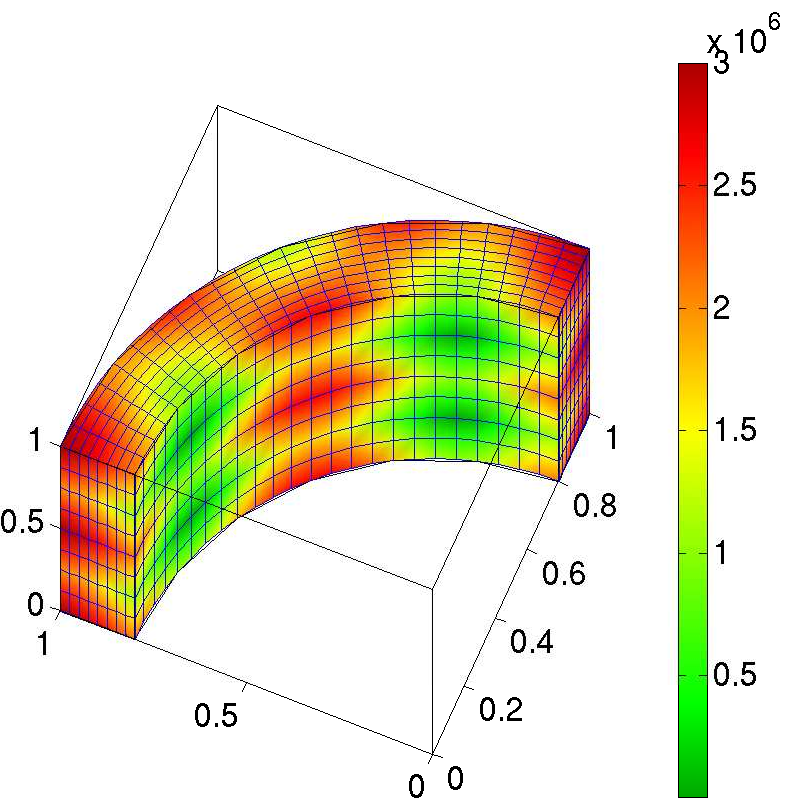
\includegraphics[width=0.48\textwidth]{figs/fan3a}
	\caption{\label{fig:mesh} Two and three dimensional warped
          meshes used in our numerical experiments. The color
          illustrates the value of the coefficient $\mu(\bs x)$.}
\end{figure}


\subsection{Setup of comparisons}\label{subsec:measures}
Tables \ref{tab:box}--\ref{tab:3d-fan} present the number of multigrid
v-cycles or of conjugate gradient (CG) iterations required to reduce
the norm of the discrete residual by a factor of $10^8$. In
particular, these tables report the following.
\begin{itemize}
\item[$\bullet$] The first column gives the polynomial \emph{order}
  used in the finite element discretization.
\item[$\bullet$] The columns entitled by \emph{MG as solver} report
  the number of v-cycles needed when multigrid is used as a
  solver. The subcolums are:
  \begin{itemize}
  \item \emph{Jacobi(3,3)} denotes that 3 pre-smoothing and 3
    post-smoothing steps of a pointwise Jacobi smoother are used on
    each level.
  \item \emph{Cheb(3,3)} indicates that Chebyshev-accelerated Jacobi
    smoothing is used, again with 3 pre-smoothing and 3
    post-smoothing steps. The maximal eigenvalue required by the
    Chebyshev method is estimated using 10 Arnoldi iterations.
  \item \emph{SSOR(2,1)} denotes that a symmetric successive
    over-relaxation method is employed, where 2 pre-smoothing and 1
    post-smoothing step are employed. Note that each SSOR smoothing
    iteration amounts to a forward and a backward v-cycle, and thus
    requires double the computational work compared to Jacobi
    smoothing.\footnote{This ignores aspects occurring in parallel
      environments, where Gauss-Seidel smoothing---such as SSOR---can
      be challenging to implement and requires more communication in
      distributed memory environments.}. The SSOR smoother is based on 
			a lexicographic ordering of  the unknowns. 
  \end{itemize}
  \item For the 2D meshes, Tables~\ref{tab:box}-\ref{tab:2d-fan}, we use 
  three $h$-grids of sizes $32\times32$, $16\times16$ and $8\times8$. For 
  the 3D meshes, Tables~\ref{tab:3d-box}-\ref{tab:3d-fan}, we use grids of 
  sizes $8\times8\times8$, $4\times4\times4$ and $2\times2\times2$.
  Note that for each smoother we report results for
  $h$-multigrid (columns marked by \emph{h}; see
  \S\ref{subsec:h}) as well as for $p$-multigrid (columns marked
  by \emph{p}; see \S\ref{subsec:p}). For $p$-multigrid, we
  restrict ourselves to orders that are powers of 2. After
  coarsening in $p$ till $p=1$, we coarsen in $h$. For example in the 2D case, 
  for $p=16$, we will have a total of 7 grids; the first 5 shall be grids of 
  size $32\times32\times32$ with $p=16,8,4,2,1$, respectively, followed by 
  two additional coarse grids of size $16\times16$ and $8\times8$ and $p=1$.
\item[$\bullet$] The columns entitled \emph{MG with pCG} presents our
  results obtained when multigrid is uses as preconditioner in a CG
  algorithm. A single multigrid v-cycle is used per CG iteration. The sub-columns 
  again correspond to different smoothers, as described above.
\item[$\bullet$] The columns headed by \emph{linearized pCG} present
  the number of CG iterations needed to solve the high-order system
  preconditioned with the low-order operator based on the high-order
  node points (see \S\ref{subsec:low}). While in practice one
  would most likely use an algebraic multigrid cycle to approximately
  solve the linearized system, here we use a direct factorization
  method as solver for the low-order system. The different columns
  correspond to different numbers of Chebyshev-accelerated Jacobi
  smoothing steps on the finest mesh. These smoothing steps use the
  high-order residual but the diagonal from the low-order system. As a
  consequence, the Chebyshev smoother requires an estimate of the
  largest eigenvalue of the high-order matrix preconditioned with the
  diagonal of the low-order operator, which is computed using
  10 iterations of the Arnoldi algorithm.
\end{itemize}
In the next section, we summarize our numerical comparisons.

\subsection{Summary of numerical results}\label{subsec:results}
The Tables \ref{tab:box} and \ref{tab:2d-fan} present our results for
the two dimensional test problems. As can be seen in
Table~\ref{tab:box}, for the Laplace problem on the unit square all
solver/smoothing variants converge for all polynomial orders in a
relatively small number of iterations. However, the number of
iterations increases with the polynomial orders $p$, in particular
when multigrid is used as a solver. Using multigrid as a
preconditioner in CG results in a reduction of multigrid v-cycles, in
some cases even by a factor or two. Also, we observe that SSOR
smoothing generally performs better than the two Jacobi-based
smoothers. We find that the linear-order operator based on the
high-order nodes is a good preconditioner for the high-order
system. The convergence of this method is significantly improved when
smoothing steps on the finest level are used. Note that the Jacobi
smoother underlying the Chebyshev smoother uses the diagonal entries
of the low-order operator, but the residual computed from the
high-order operator. The low-order preconditioning approach proves to
be efficient, making it particularly attractive for high-order
discretized problems on unstructured meshes. However, in our tests
this efficiency partly has to be attributed to the use of a direct
solver for the low-order system, rather than an approximate solution
based on an algebraic multigrid method.

% \gsnote{It's interesting that with 3 smoothing steps this
%  performs better than the high-order multigrid with Chebyshev
%  smoother---the computational work is comparable; but I think this
%  might be caused by the direct solves on the coarse level.}

\begin{table}
  \caption{\label{tab:box} Results for two-dimensional unit square
    with constant coefficient $\mu\equiv 1$.  A total of 3 grids were
    used, the finest grid was $32\times 32$, and the coarsest was
    $8\times 8$. For a detailed description of the different
    experiments reported in this table we refer to
    \S\ref{subsec:measures}.}  \centering
  \begin{tabular}{|r|c c|c c|c c||c c|c c|c c||c c c|} 
    \hline
    & \multicolumn{6}{c||}{MG as solver} & \multicolumn{6}{c||}{MG with pCG} & \multicolumn{3}{r|}{linearized} \\
    \cline{2-13}
    \!\!\! order \!\!\!\! &  \multicolumn{2}{c|}{\!\scriptsize  Jacobi(3)\!} &  \multicolumn{2}{c|}{\!\scriptsize Cheb(3)\!} & \multicolumn{2}{c||}{\!\scriptsize  SSOR(2)\!} & \multicolumn{2}{c|}{\!\scriptsize Jacobi(3)\!} &  \multicolumn{2}{c|}{\!\scriptsize Cheb(3)\!} & \multicolumn{2}{c||}{\!\scriptsize SSOR(2)\!} & \multicolumn{3}{c|}{pCG}\\
\hline
 & $h$ & $p$ & $h$ & $p$& $h$ & $p$& $h$ & $p$& $h$ & $p$& $h$ & $p$& 0 & 1 & 3\\
 \cline{2-16}
1 & 6 & & 5 & & 5 & & 5 & & 4 & & 4 & & - & - & - \\
2 & 7 & 7 & 5 & 6 & 5 & 5 & 5 & 5 & 4 & 4 & 4 & 4 & 14 & 9 & 4 \\
3 & 8 & & 6 & & 5 & & 6 & & 5 & & 4 & & 16 & 9 & 4 \\
4 & 9 & 8 & 6 & 6 & 5 & 5 & 6 & 5 & 5 & 5 & 4 & 4 & 16 & 10 & 4 \\
5 & 12 & & 8 & & 7 & & 7 & & 6 & & 5 & & 17 & 10 & 4 \\
6 & 12 & & 9 & & 7 & & 7 & & 6 & & 5 & & 18 & 11 & 5\\
7 & 16 & & 12 & & 8 & & 8 & & 7 & & 6 & & 18 & 12 & 5 \\
8 & 17 & 14 & 13 & 10 & 8 & 7 & 9 & 8 & 7 & 6 & 6 & 5 & 19 & 12 & 5\\
16 & 40 & 33 & 33 & 27 & 17 & 14 & 14 & 12 & 12 & 11 & 9 & 8 & 21 & 14 & 8 \\
\hline
  \end{tabular}
\end{table}


Let us now contrast these observations with the results for the
variable coefficient case summarized in Table~\ref{tab:2d-fan}. First,
note that all variants perform reasonably for discretizations up to
order $p=4$. When used as a solver, multigrid either diverges or
converges very slowly for orders $p>4$. Convergence is reestablished
when multigrid is combined with CG.

Next, we turn to the three dimensional results reported in
Tables~\ref{tab:3d-box} and \ref{tab:3d-fan}. All of our
multigrid/smoother variants converge for the Laplace equation on the
unit cube, as shown in Table~\ref{tab:3d-box}. The benefit of using
multigrid as preconditioner rather than as solver is even more evident
in three dimensions than for the two dimensional unit square
problem. \todo{Need to comment on linearized preconditioner.}

Our results for varying coefficient problem on the three-dimensional
geometry shown in Figure~\ref{fig:mesh} are summarized in
Table~\ref{tab:3d-fan}. As in two dimensions, the performance of
multigrid when used as a solver degrades significantly for orders
$p>4$.


\begin{table}
  \caption{\label{tab:2d-fan} Results for two-dimensional warped
    geometry with varying coefficient $\mu(x,y) = 1 + 10^6(\cos^2(2\pi
    x) + \cos^2(2\pi y))$.  A total of 3 grids were used, the finest
    grid was $32\times 32$, and the coarsest was $8\times 8$. For a
    detailed description of the different experiments reported in this
    table we refer to \S\ref{subsec:measures}.}  \centering
  \begin{tabular}{|r|c c|c c|c c||c c|c c|c c||c c c|} 
    \hline
    & \multicolumn{6}{c||}{MG as solver} & \multicolumn{6}{c||}{MG with pCG} & \multicolumn{3}{r|}{linearized} \\
    \cline{2-13}
    \!\!\! order \!\!\!\! &  \multicolumn{2}{c|}{\!\scriptsize  Jacobi(3)\!} &  \multicolumn{2}{c|}{\!\scriptsize Cheb(3)\!} & \multicolumn{2}{c||}{\!\scriptsize  SSOR(2)\!} & \multicolumn{2}{c|}{\!\scriptsize Jacobi(3)\!} &  \multicolumn{2}{c|}{\!\scriptsize Cheb(3)\!} & \multicolumn{2}{c||}{\!\scriptsize SSOR(2)\!} & \multicolumn{3}{c|}{pCG}\\
\hline
 & $h$ & $p$ & $h$ & $p$& $h$ & $p$& $h$ & $p$& $h$ & $p$& $h$ & $p$& 0 & 1 & 3\\
 \cline{2-16}
1 & 14 & & 11 & & 6 & & 8 & & 7 & & 5 & & - & - & - \\
2 & 20 & 19 & 15 & 15 & 7 & 8 & 10 & 10 & 8 & 8 & 5 & 6 & 16 & 9 & 5 \\
3 & 20 & & 16 & & 8 & & 10 & & 9 & & 6 & & 18 & 9 & 6 \\
4 & 22 & 21 & 21 & 19 & 10 & 9 & 11 & 10 & 10 & 10 & 7 & 6 & 19 & 11 & 7\\
5 & -  & & 28 & & 12 & & 14 & & 12 & & 7 & & 21 & 12 & 8  \\
6 & -  & & 35 & & 13 & & 15 & & 13 & & 8 & & 23 & 13 & 9 \\
7 & -  & & 45 & & 16 & & 18 & & 15 & & 9 & & 24 & 14 & 9 \\
8 & -  & - & 52 & 46 & 17 & 15 & 20 & 20 & 16 & 15 & 9 & 8 & 25 & 14 & 10 \\
16 & - & - & 169 & 148 & 37 & 33 & 51 & 45 & 30 & 27 & 13 & 12 & 31 & 19 & 13 \\
\hline
  \end{tabular}
\end{table}


\begin{table}
  \caption{\label{tab:3d-box} Results for three-dimensional cube
    geometry with constant coefficient $\mu(\bs x) \equiv 1$. For a
    detailed description of the different experiments reported in this
    table we refer to \S\ref{subsec:measures}.}  \centering
	  \begin{tabular}{|r|c c|c c|c c||c c|c c|c c||c c c|} 
	    \hline
	    & \multicolumn{6}{c||}{MG as solver} & \multicolumn{6}{c||}{MG with pCG} & \multicolumn{3}{r|}{linearized} \\
	    \cline{2-13}
	    \!\!\! order \!\!\!\! &  \multicolumn{2}{c|}{\!\scriptsize  Jacobi(3)\!} &  \multicolumn{2}{c|}{\!\scriptsize Cheb(3)\!} & \multicolumn{2}{c||}{\!\scriptsize  SSOR(2)\!} & \multicolumn{2}{c|}{\!\scriptsize Jacobi(3)\!} &  \multicolumn{2}{c|}{\!\scriptsize Cheb(3)\!} & \multicolumn{2}{c||}{\!\scriptsize SSOR(2)\!} & \multicolumn{3}{c|}{pCG}\\
	\hline
	 & $h$ & $p$ & $h$ & $p$& $h$ & $p$& $h$ & $p$& $h$ & $p$& $h$ & $p$& 0 & 1 & 3\\
	 \cline{2-16}
1 & 6 & & 4 & & 4 & & 5 & & 4 & & 3 & & - & - & - \\
2 & 8 & 8 & 4 & 5 & 4 & 5 & 6 & 6 & 4 & 4 & 4 & 4 &  25 & 14 & 5 \\
3 & 10 & & 7 & & 5 & & 6 & & 5 & & 5 & & 27 & 13 & 5  \\
4 & 11 & 10 & 8 & 7 & 6 & 5 & 7 & 7 & 6 & 5 & 5 & 4 & 28 & 15 & 6 \\
5 & 14 & & 10 & & 7 & & 8 & & 7 & & 5 & & 29 & 16 & 6 \\
6 & 16 & & 11 & & 7 & & 9 & & 7 & & 6 & & 32 & 18 & 6 \\
7 & 20 & & 15 & & 9 & & 10 & & 9 & & 6 & & 34 & 19 & 7 \\
8 & 22 & 19 & 17 & 15 & 9 & 8 & 10 & 10 & 9 & 8 & 6 & 6 & 35 & 20 & 7 \\
16 & 47 & 42 & 38 & 34 & 17 & 15 & 16 & 14 & 14 & 13 & 9 & 9 & 39 & 22 & 11 \\
\hline 
 \end{tabular}
\end{table}

\begin{table}
  \caption{\label{tab:3d-fan} Results for three-dimensional warped
    geometry with varying coefficient $\mu(x,y,z) = 1 +
    10^6(\cos^2(2\pi x) + \cos^2(2\pi y) + \cos^2(2\pi z))$. For a
    detailed description of the different experiments reported in this
    table we refer to \S\ref{subsec:measures}.}  \centering
	  \begin{tabular}{|r|c c|c c|c c||c c|c c|c c||c c c|} 
	    \hline
	    & \multicolumn{6}{c||}{MG as solver} & \multicolumn{6}{c||}{MG with pCG} & \multicolumn{3}{r|}{linearized} \\
	    \cline{2-13}
	    \!\!\! order \!\!\!\! &  \multicolumn{2}{c|}{\!\scriptsize  Jacobi(3)\!} &  \multicolumn{2}{c|}{\!\scriptsize Cheb(3)\!} & \multicolumn{2}{c||}{\!\scriptsize  SSOR(2)\!} & \multicolumn{2}{c|}{\!\scriptsize Jacobi(3)\!} &  \multicolumn{2}{c|}{\!\scriptsize Cheb(3)\!} & \multicolumn{2}{c||}{\!\scriptsize SSOR(2)\!} & \multicolumn{3}{c|}{pCG}\\
	\hline
	 & $h$ & $p$ & $h$ & $p$& $h$ & $p$& $h$ & $p$& $h$ & $p$& $h$ & $p$& 0 & 1 & 3\\
	 \cline{2-16}
1 & 13 & & 7 & & 5 & & 7 & & 5 & & 4 & & - & - & - \\
2 & 17 & 18 & 13 & 13 & 7 & 7 & 9 & 9 & 8 & 8 & 5 & 5 & 26 & 14 & 7 \\
3 & 20 & & 16 & & 8 & & 10 & & 9 & & 6 & & 29 & 14 & 8 \\
4 & 23 & 22 & 18 & 18 & 9 & 9 & 11 & 11 & 9 & 9 & 7 & 6 & 31 & 16 & 9\\
5 & 26 & & 21 & & 10 & & 12 & & 10 & & 7 & & 34 & 17 & 10  \\
6 & 30 & & 27 & & 12 & & 13 & & 12 & & 8 & & 37 & 20 & 13 \\
7 & 35 & & 34 & & 14 & & 14 & & 14 & & 8 & & 37 & 21 & 13  \\
8 & - & - & 40 & 38 & 16 & 15 & 18 & 17 & 15 & 14 & 9 & 9 & 38 & 21 & 14 \\
16 & - & - & 117 & 110 & 32 & 29 & 67 & 60 & 27 & 26 & 13 & 13 & 47 & 28 & 22 \\
\hline
  \end{tabular}
\end{table}

In the next section, we summarize our findings and draw conclusions.

\section{Discussion and conclusions}
\label{sec:discuss}

Despite the fact that discrete systems originating from high-order
discretizations do not satisfy favorable matrix properties such as the
M-matrix property, we find that point smoothers can be efficient for
polynomial orders up to $p=16$.  For constant coefficient, two and
three-dimensional problems, all tested point smoothers (Jacobi,
Chebyshev-accelerated Jacobi and Gauss-Seidel SSOR smoothing) lead to
converging multigrid methods. For highly varying coefficients on
deformed geometries, SSOR outperforms Jacobi-based smoothing, which
performs poorly for orders $p>4$.

In a parallel environment, where Gauss-Seidel smoothing is
significantly more difficult to implement and requires more parallel
communication, Chebyshev-accelerated Jacobi smoothing represents an
interesting alternative since it is as simple to implement as Jacobi
smoothing.

Using multigrid as preconditioner in a Krylov method rather than as
solver results in significantly faster convergence, which by far
compensates for the additional work required by the Krylov method,
namely vector additions and inner products.  For problems with varying
coefficients, we found that the number of required v-cycles decreases
by up to a factor of three when combining multigrid with the conjugate
gradient method.

We find that a low order operator based on the high-order node points
is an excellent preconditioner for the low-order system, in particular
when combined with smoothing based on the high-order residual is
performed on the finest mesh.  When combined with algebraic multigrid
for the low-order operator, this approach is attractive for high-order
discretizations on unstructured meshes as also shown in
~\cite{Brown10, DevilleMund90, HeysManteuffelMcCormickEtAl05}.


%low-order preconditioner competitive w.r. to number of
%  iterations; thus a good option as preconditioner when using AMG for
%  unstructured high-order meshes

\section*{Acknowledgments}
We would like to thank Tobin Isaac for helpful discussions on the
low-order preconditioner. Support for this work was
  provided through the U.S.~National Science Foundation (NSF) grants
  CMMI-1028889 and   % CDI mantle/wave
  ARC-0941678,       % NSF ice
 and through the Scientific Discovery through Advanced
  Computing (SciDAC) projects 
  DE-SC0009286,   % Diamond
%  DE-SC0006656,  % Quest
  and DE-SC0002710 % UQ ice
  funded by the U.S.~Department of Energy
  Office of Science, Advanced Scientific Computing Research and
  Biological and Environmental Research.
 \todo{Check with George and Omar; these are Diamond, DOE ice, NSF ice and NSF mantle/wave.}


\bibliographystyle{siam}
\bibliography{ccgo}


\end{document}
